\documentclass[a4paper]{book}
\usepackage{makeidx}
\usepackage{graphicx}
\usepackage{multicol}
\usepackage{float}
\usepackage{listings}
\usepackage{color}
\usepackage{ifthen}
\usepackage[table]{xcolor}
\usepackage{textcomp}
\usepackage{alltt}
\usepackage{ifpdf}
\ifpdf
\usepackage[pdftex,
            pagebackref=true,
            colorlinks=true,
            linkcolor=blue,
            unicode
           ]{hyperref}
\else
\usepackage[ps2pdf,
            pagebackref=true,
            colorlinks=true,
            linkcolor=blue,
            unicode
           ]{hyperref}
\usepackage{pspicture}
\fi
\usepackage[utf8]{inputenc}
\usepackage{mathptmx}
\usepackage[scaled=.90]{helvet}
\usepackage{courier}
\usepackage{sectsty}
\usepackage[titles]{tocloft}
\usepackage{doxygen}
\lstset{language=C++,inputencoding=utf8,basicstyle=\footnotesize,breaklines=true,breakatwhitespace=true,tabsize=8,numbers=left }
\makeindex
\setcounter{tocdepth}{3}
\renewcommand{\footrulewidth}{0.4pt}
\renewcommand{\familydefault}{\sfdefault}
\begin{document}
\hypersetup{pageanchor=false}
\begin{titlepage}
\vspace*{7cm}
\begin{center}
{\Large MultiBoost }\\
\vspace*{1cm}
{\large Generated by Doxygen 1.7.4}\\
\vspace*{0.5cm}
{\small Fri Jul 27 2012 16:24:11}\\
\end{center}
\end{titlepage}
\clearemptydoublepage
\pagenumbering{roman}
\tableofcontents
\clearemptydoublepage
\pagenumbering{arabic}
\hypersetup{pageanchor=true}
\chapter{MultiBoost Doxygen Documentation}
\label{index}\hypertarget{index}{}\hypertarget{index_intro_sec}{}\section{Introduction}\label{index_intro_sec}
\href{http://www.multiboost.com}{\tt MultiBoost} package is a fast C++ implementation of multi-\/class/multi-\/label/multi-\/task boosting algorithms. It is based on AdaBoost.MH but also implements popular cascade classifiers and FilterBoost. The package contains common multi-\/class base learners (stumps, trees, products, Haar filters). Further base learners and strong learners following the boosting paradigm can be easily implemented in a flexible framework. Feel free to use it and to modify it!

This software is covered by the \href{http://www.gnu.org/copyleft/lesser.html}{\tt LGPL} licence.\hypertarget{index_install_sec}{}\section{Installation}\label{index_install_sec}
Execute the following command in the directory where the zipped source code is located in order to compile :


\begin{DoxyCode}
 % unzip multiboost.zip
 % cmake .
 % make
\end{DoxyCode}


Note: you need \href{http://www.cmake.org}{\tt cmake} to create the Makefile. To run the program, just type: 
\begin{DoxyCode}
 % multiboost
\end{DoxyCode}


To get some help, type: 
\begin{DoxyCode}
 % multiboost -help
\end{DoxyCode}
\hypertarget{index_Basic}{}\section{Coding Informations}\label{index_Basic}
MultiBoost was built with Boosting algorithms in mind, in particular for multi-\/class AdaBoost.MH.

The concept has been centered on the base learner (aka weak learner), which holds the methods to find the best function h(x) at each boosting iteration. Each base function can also decide the type of data to process, and even the strong learner that is calling it.

Here is how it works:\par
 \begin{DoxyItemize}
\item Each base learner (i.e. \hyperlink{classMultiBoost_1_1SingleStumpLearner}{SingleStumpLearner}) is registered in a static list, that is a class factory, using just a simple macro (see \hyperlink{BaseLearner_8h_a784f5b7d276202c7de7108eeca341da7}{REGISTER\_\-LEARNER} for details). \item The users selects the base learner either by providing an argument on the command line or by loading a strong hypothesis file. \item If the base learner is in the static list, it will inform the framework what are its InputData and \hyperlink{classMultiBoost_1_1GenericStrongLearner}{GenericStrongLearner}. If the default data format (\hyperlink{classMultiBoost_1_1InputData}{InputData}) and strong learner (\hyperlink{classMultiBoost_1_1AdaBoostMHLearner}{AdaBoostMHLearner}) are not enough they can be overrided with two methods of \hyperlink{classMultiBoost_1_1BaseLearner}{BaseLearner}: \hyperlink{classMultiBoost_1_1BaseLearner_aa6bce26112ef2ce1275385d06467a9a9}{createInputData()} and \hyperlink{classMultiBoost_1_1BaseLearner_a80735a2e6adfc75e52bad70a0072d890}{createGenericStrongLearner()}. \item The strong learner run the boosting process by creating an object of type BaseLearner (any registered weak learner must implement the method subCreate() which returns an allocated copy of itself), that will have to find the best h(x) for the current boosting iteration. Once the function has been received it is stored in the vector of the weak learner. Note that the weighting factor alpha (if needed) needs to be stored in the weak learner. \item The serialization is performed simply by overriding the proper classes of \hyperlink{classMultiBoost_1_1BaseLearner}{BaseLearner}. \item The classification depends on the strong learner chosen. can classify any type of weak learner that use AdaBoost.MH as strong learner, as long as they implement all the abstract methods.\end{DoxyItemize}
For any other question, please refer to the documentation or contact one of the authors.\hypertarget{index_References}{}\section{References}\label{index_References}
Here's the {\bfseries bibtex} reference: \begin{DoxyVerb}
 @article{multiboost,
 title={Multiboost: a multi-purpose boosting package},
 author={Benbouzid, D. and Busa-Fekete, R. and Casagrande, N. and Collin, F.D. and K{\'e}gl, B.},
 journal={Journal of Machine Learning Research},
 volume={13},
 pages={549--553},
 year={2012}
 }\end{DoxyVerb}
 
\chapter{Todo List}
\label{todo}
\hypertarget{todo}{}

\begin{DoxyRefList}
\item[\label{todo__todo000002}%
\hypertarget{todo__todo000002}{}%
Class \hyperlink{classMultiBoost_1_1BaseLearner}{Multi\-Boost\-:\-:Base\-Learner} ]Add a get\-Alpha for non-\/binary (ternary) base-\/classifiers, using line-\/search.  
\item[\label{todo__todo000003}%
\hypertarget{todo__todo000003}{}%
Member \hyperlink{classMultiBoost_1_1HaarFeature_a27de701185caaff11713083941f9880e}{Multi\-Boost\-:\-:Haar\-Feature\-:\-:move\-To\-Next\-Config} ()]Replace the \char`\"{}visited\char`\"{} list with something less awful.  
\item[\label{todo__todo000001}%
\hypertarget{todo__todo000001}{}%
Member \hyperlink{classMultiBoost_1_1SortedData_a4026ff8765982ac0c0edff12a929917f}{Multi\-Boost\-:\-:Sorted\-Data\-:\-:load} (const string \&file\-Name, e\-Input\-Type input\-Type=I\-T\-\_\-\-T\-R\-A\-I\-N, int verbose\-Level=1)]Erase the original memory once sorted? 
\end{DoxyRefList}
\chapter{Bug List}
\label{bug}
\hypertarget{bug}{}

\begin{DoxyRefList}
\item[\label{bug__bug000002}%
\hypertarget{bug__bug000002}{}%
Member \hyperlink{classMultiBoost_1_1AbstainableLearner_a04438bf3df3599fe42ca26771b6b2aff}{Multi\-Boost\-:\-:Abstainable\-Learner\-:\-:do\-Real\-Abstention} (const vector$<$ s\-Rates $>$ \&mu, const s\-Rates \&eps, Alpha\-Real \&alpha, vector$<$ Alpha\-Real $>$ \&v)]The actual formula should be \[ Z = \mu_0 + 2 \sum_{\ell=1}^k \sqrt{ \mu_{-,\ell} \mu_{+,\ell} }, \] but we do not consider the abstention at weak learner level yet.  
\item[\label{bug__bug000001}%
\hypertarget{bug__bug000001}{}%
Member \hyperlink{classnor__utils_1_1StreamTokenizer_a16acf21421cefcc3c45c54eb0ac8810e}{nor\-\_\-utils\-:\-:Stream\-Tokenizer\-:\-:has\-\_\-token} ()]In fact this method does not know if there are other tokens awaiting. If there are characters after the last delimiter at the end of the stream, they will be considered a token and therefore, this method will return true. This happens also if there is just a newline (in the case it is not a delimiter). It is possible to avoid this problem, but will affect efficency. Because a \char`\"{}spurious\char`\"{} token will just be ignored by the parser I decided to just leave it as it is. 
\end{DoxyRefList}
\chapter{Class Index}
\section{Class Hierarchy}
This inheritance list is sorted roughly, but not completely, alphabetically:\begin{DoxyCompactList}
\item \contentsline{section}{MultiBoost::AdaBoostMHClassifier}{\pageref{classMultiBoost_1_1AdaBoostMHClassifier}}{}
\item \contentsline{section}{nor\_\-utils::Args}{\pageref{classnor__utils_1_1Args}}{}
\item \contentsline{section}{MultiBoost::BanditSingleSparseStump}{\pageref{classMultiBoost_1_1BanditSingleSparseStump}}{}
\item \contentsline{section}{MultiBoost::BaseLearner}{\pageref{classMultiBoost_1_1BaseLearner}}{}
\begin{DoxyCompactList}
\item \contentsline{section}{MultiBoost::AbstainableLearner}{\pageref{classMultiBoost_1_1AbstainableLearner}}{}
\begin{DoxyCompactList}
\item \contentsline{section}{MultiBoost::ConstantLearner}{\pageref{classMultiBoost_1_1ConstantLearner}}{}
\item \contentsline{section}{MultiBoost::FeaturewiseLearner}{\pageref{classMultiBoost_1_1FeaturewiseLearner}}{}
\begin{DoxyCompactList}
\item \contentsline{section}{MultiBoost::IndicatorLearner}{\pageref{classMultiBoost_1_1IndicatorLearner}}{}
\item \contentsline{section}{MultiBoost::MultiThresholdStumpLearner}{\pageref{classMultiBoost_1_1MultiThresholdStumpLearner}}{}
\item \contentsline{section}{MultiBoost::OneClassStumpLearner}{\pageref{classMultiBoost_1_1OneClassStumpLearner}}{}
\item \contentsline{section}{MultiBoost::SelectorLearner}{\pageref{classMultiBoost_1_1SelectorLearner}}{}
\item \contentsline{section}{MultiBoost::SigmoidSingleStumpLearner}{\pageref{classMultiBoost_1_1SigmoidSingleStumpLearner}}{}
\item \contentsline{section}{MultiBoost::SingleRegressionStumpLearner}{\pageref{classMultiBoost_1_1SingleRegressionStumpLearner}}{}
\item \contentsline{section}{MultiBoost::SingleSparseStump}{\pageref{classMultiBoost_1_1SingleSparseStump}}{}
\item \contentsline{section}{MultiBoost::SingleStumpLearner}{\pageref{classMultiBoost_1_1SingleStumpLearner}}{}
\begin{DoxyCompactList}
\item \contentsline{section}{MultiBoost::HaarSingleStumpLearner}{\pageref{classMultiBoost_1_1HaarSingleStumpLearner}}{}
\item \contentsline{section}{MultiBoost::OneClassStumpLearner}{\pageref{classMultiBoost_1_1OneClassStumpLearner}}{}
\item \contentsline{section}{MultiBoost::SingleSparseStumpLearner}{\pageref{classMultiBoost_1_1SingleSparseStumpLearner}}{}
\item \contentsline{section}{MultiBoost::UCBVHaarSingleStumpLearner}{\pageref{classMultiBoost_1_1UCBVHaarSingleStumpLearner}}{}
\end{DoxyCompactList}
\end{DoxyCompactList}
\item \contentsline{section}{MultiBoost::MultiStumpLearner}{\pageref{classMultiBoost_1_1MultiStumpLearner}}{}
\begin{DoxyCompactList}
\item \contentsline{section}{MultiBoost::HaarMultiStumpLearner}{\pageref{classMultiBoost_1_1HaarMultiStumpLearner}}{}
\end{DoxyCompactList}
\item \contentsline{section}{MultiBoost::NeuronLearner}{\pageref{classMultiBoost_1_1NeuronLearner}}{}
\begin{DoxyCompactList}
\item \contentsline{section}{MultiBoost::AdaLineLearner}{\pageref{classMultiBoost_1_1AdaLineLearner}}{}
\end{DoxyCompactList}
\end{DoxyCompactList}
\item \contentsline{section}{MultiBoost::BanditLearner}{\pageref{classMultiBoost_1_1BanditLearner}}{}
\item \contentsline{section}{MultiBoost::ParasiteLearner}{\pageref{classMultiBoost_1_1ParasiteLearner}}{}
\item \contentsline{section}{MultiBoost::ProductLearner}{\pageref{classMultiBoost_1_1ProductLearner}}{}
\item \contentsline{section}{MultiBoost::ProductLearnerUCT}{\pageref{classMultiBoost_1_1ProductLearnerUCT}}{}
\item \contentsline{section}{MultiBoost::ScalarLearner}{\pageref{classMultiBoost_1_1ScalarLearner}}{}
\begin{DoxyCompactList}
\item \contentsline{section}{MultiBoost::ConstantLearner}{\pageref{classMultiBoost_1_1ConstantLearner}}{}
\item \contentsline{section}{MultiBoost::IndicatorLearner}{\pageref{classMultiBoost_1_1IndicatorLearner}}{}
\item \contentsline{section}{MultiBoost::OneClassStumpLearner}{\pageref{classMultiBoost_1_1OneClassStumpLearner}}{}
\item \contentsline{section}{MultiBoost::SelectorLearner}{\pageref{classMultiBoost_1_1SelectorLearner}}{}
\item \contentsline{section}{MultiBoost::SigmoidSingleStumpLearner}{\pageref{classMultiBoost_1_1SigmoidSingleStumpLearner}}{}
\item \contentsline{section}{MultiBoost::SingleSparseStump}{\pageref{classMultiBoost_1_1SingleSparseStump}}{}
\item \contentsline{section}{MultiBoost::SingleStumpLearner}{\pageref{classMultiBoost_1_1SingleStumpLearner}}{}
\end{DoxyCompactList}
\item \contentsline{section}{MultiBoost::StochasticLearner}{\pageref{classMultiBoost_1_1StochasticLearner}}{}
\begin{DoxyCompactList}
\item \contentsline{section}{MultiBoost::AdaLineLearner}{\pageref{classMultiBoost_1_1AdaLineLearner}}{}
\item \contentsline{section}{MultiBoost::ConstantLearner}{\pageref{classMultiBoost_1_1ConstantLearner}}{}
\item \contentsline{section}{MultiBoost::SigmoidSingleStumpLearner}{\pageref{classMultiBoost_1_1SigmoidSingleStumpLearner}}{}
\end{DoxyCompactList}
\item \contentsline{section}{MultiBoost::TreeLearner}{\pageref{classMultiBoost_1_1TreeLearner}}{}
\item \contentsline{section}{MultiBoost::TreeLearnerUCT}{\pageref{classMultiBoost_1_1TreeLearnerUCT}}{}
\end{DoxyCompactList}
\item \contentsline{section}{MultiBoost::BaseOutputInfoType}{\pageref{classMultiBoost_1_1BaseOutputInfoType}}{}
\begin{DoxyCompactList}
\item \contentsline{section}{MultiBoost::AUCOutput}{\pageref{classMultiBoost_1_1AUCOutput}}{}
\item \contentsline{section}{MultiBoost::BalancedErrorOutput}{\pageref{classMultiBoost_1_1BalancedErrorOutput}}{}
\item \contentsline{section}{MultiBoost::EdgeOutput}{\pageref{classMultiBoost_1_1EdgeOutput}}{}
\item \contentsline{section}{MultiBoost::HammingErrorOutput}{\pageref{classMultiBoost_1_1HammingErrorOutput}}{}
\item \contentsline{section}{MultiBoost::MAEOuput}{\pageref{classMultiBoost_1_1MAEOuput}}{}
\item \contentsline{section}{MultiBoost::MarginsOutput}{\pageref{classMultiBoost_1_1MarginsOutput}}{}
\item \contentsline{section}{MultiBoost::PosteriorsOutput}{\pageref{classMultiBoost_1_1PosteriorsOutput}}{}
\item \contentsline{section}{MultiBoost::RestrictedZeroOneError}{\pageref{classMultiBoost_1_1RestrictedZeroOneError}}{}
\item \contentsline{section}{MultiBoost::SoftCascadeOutput}{\pageref{classMultiBoost_1_1SoftCascadeOutput}}{}
\item \contentsline{section}{MultiBoost::TPRFPROutput}{\pageref{classMultiBoost_1_1TPRFPROutput}}{}
\item \contentsline{section}{MultiBoost::VJCascadeOutput}{\pageref{classMultiBoost_1_1VJCascadeOutput}}{}
\item \contentsline{section}{MultiBoost::WeightedErrorOutput}{\pageref{classMultiBoost_1_1WeightedErrorOutput}}{}
\item \contentsline{section}{MultiBoost::WeightedHammingErrorOutput}{\pageref{classMultiBoost_1_1WeightedHammingErrorOutput}}{}
\item \contentsline{section}{MultiBoost::WeightedZeroOneErrorOutput}{\pageref{classMultiBoost_1_1WeightedZeroOneErrorOutput}}{}
\item \contentsline{section}{MultiBoost::ZeroOneErrorOutput}{\pageref{classMultiBoost_1_1ZeroOneErrorOutput}}{}
\end{DoxyCompactList}
\item \contentsline{section}{BitStream}{\pageref{structBitStream}}{}
\item \contentsline{section}{bz\_\-stream}{\pageref{structbz__stream}}{}
\item \contentsline{section}{bzFile}{\pageref{structbzFile}}{}
\item \contentsline{section}{Bzip2WrapperReader}{\pageref{classBzip2WrapperReader}}{}
\item \contentsline{section}{Bzip2WrapperWriter}{\pageref{classBzip2WrapperWriter}}{}
\item \contentsline{section}{MultiBoost::CascadeOutputInformation}{\pageref{structMultiBoost_1_1CascadeOutputInformation}}{}
\item \contentsline{section}{MultiBoost::ClassHierarchy}{\pageref{classMultiBoost_1_1ClassHierarchy}}{}
\item \contentsline{section}{nor\_\-utils::comparePair$<$ 1, T1, T2, Pred $>$}{\pageref{structnor__utils_1_1comparePair_3_011_00_01T1_00_01T2_00_01Pred_01_4}}{}
\item \contentsline{section}{nor\_\-utils::comparePair$<$ 2, T1, T2, Pred $>$}{\pageref{structnor__utils_1_1comparePair_3_012_00_01T1_00_01T2_00_01Pred_01_4}}{}
\item \contentsline{section}{nor\_\-utils::comparePairP$<$ 1, T1, T2, Pred $>$}{\pageref{structnor__utils_1_1comparePairP_3_011_00_01T1_00_01T2_00_01Pred_01_4}}{}
\item \contentsline{section}{nor\_\-utils::comparePairP$<$ 2, T1, T2, Pred $>$}{\pageref{structnor__utils_1_1comparePairP_3_012_00_01T1_00_01T2_00_01Pred_01_4}}{}
\item \contentsline{section}{MultiBoost::ConstantAlgorithm}{\pageref{classMultiBoost_1_1ConstantAlgorithm}}{}
\item \contentsline{section}{MultiBoost::ConstantAlgorithmLSHTC}{\pageref{classMultiBoost_1_1ConstantAlgorithmLSHTC}}{}
\item \contentsline{section}{DState}{\pageref{structDState}}{}
\item \contentsline{section}{EState}{\pageref{structEState}}{}
\item \contentsline{section}{MultiBoost::Example}{\pageref{classMultiBoost_1_1Example}}{}
\item \contentsline{section}{MultiBoost::ExampleResults}{\pageref{classMultiBoost_1_1ExampleResults}}{}
\item \contentsline{section}{MultiBoost::FeatureDataUCBV}{\pageref{structMultiBoost_1_1FeatureDataUCBV}}{}
\item \contentsline{section}{MultiBoost::HaarFeature::FeaturesRegs}{\pageref{classMultiBoost_1_1HaarFeature_1_1FeaturesRegs}}{}
\item \contentsline{section}{MultiBoost::GenericBanditAlgorithm}{\pageref{classMultiBoost_1_1GenericBanditAlgorithm}}{}
\begin{DoxyCompactList}
\item \contentsline{section}{MultiBoost::Exp3}{\pageref{classMultiBoost_1_1Exp3}}{}
\item \contentsline{section}{MultiBoost::Exp3G}{\pageref{classMultiBoost_1_1Exp3G}}{}
\begin{DoxyCompactList}
\item \contentsline{section}{MultiBoost::Exp3G2}{\pageref{classMultiBoost_1_1Exp3G2}}{}
\item \contentsline{section}{MultiBoost::Exp3P}{\pageref{classMultiBoost_1_1Exp3P}}{}
\end{DoxyCompactList}
\item \contentsline{section}{MultiBoost::Hedge}{\pageref{classMultiBoost_1_1Hedge}}{}
\item \contentsline{section}{MultiBoost::Random}{\pageref{classMultiBoost_1_1Random}}{}
\item \contentsline{section}{MultiBoost::UCBK}{\pageref{classMultiBoost_1_1UCBK}}{}
\begin{DoxyCompactList}
\item \contentsline{section}{MultiBoost::UCBKRandomized}{\pageref{classMultiBoost_1_1UCBKRandomized}}{}
\end{DoxyCompactList}
\item \contentsline{section}{MultiBoost::UCBKV}{\pageref{classMultiBoost_1_1UCBKV}}{}
\end{DoxyCompactList}
\item \contentsline{section}{MultiBoost::GenericBanditAlgorithmLS$<$ BaseType, KeyType $>$}{\pageref{classMultiBoost_1_1GenericBanditAlgorithmLS}}{}
\begin{DoxyCompactList}
\item \contentsline{section}{MultiBoost::Exp3LS$<$ BaseType, KeyType $>$}{\pageref{classMultiBoost_1_1Exp3LS}}{}
\begin{DoxyCompactList}
\item \contentsline{section}{MultiBoost::Exp3GLS$<$ BaseType, KeyType $>$}{\pageref{classMultiBoost_1_1Exp3GLS}}{}
\end{DoxyCompactList}
\item \contentsline{section}{MultiBoost::UCT$<$ BaseType, KeyType $>$}{\pageref{classMultiBoost_1_1UCT}}{}
\end{DoxyCompactList}
\item \contentsline{section}{MultiBoost::GenericParser}{\pageref{classMultiBoost_1_1GenericParser}}{}
\begin{DoxyCompactList}
\item \contentsline{section}{MultiBoost::ArffParser}{\pageref{classMultiBoost_1_1ArffParser}}{}
\begin{DoxyCompactList}
\item \contentsline{section}{MultiBoost::ArffParserBzip2}{\pageref{classMultiBoost_1_1ArffParserBzip2}}{}
\end{DoxyCompactList}
\item \contentsline{section}{MultiBoost::SVMLightParser}{\pageref{classMultiBoost_1_1SVMLightParser}}{}
\item \contentsline{section}{MultiBoost::TxtParser}{\pageref{classMultiBoost_1_1TxtParser}}{}
\end{DoxyCompactList}
\item \contentsline{section}{MultiBoost::GenericStrongLearner}{\pageref{classMultiBoost_1_1GenericStrongLearner}}{}
\begin{DoxyCompactList}
\item \contentsline{section}{MultiBoost::AdaBoostMHLearner}{\pageref{classMultiBoost_1_1AdaBoostMHLearner}}{}
\begin{DoxyCompactList}
\item \contentsline{section}{MultiBoost::FilterBoostLearner}{\pageref{classMultiBoost_1_1FilterBoostLearner}}{}
\end{DoxyCompactList}
\item \contentsline{section}{MultiBoost::SoftCascadeLearner}{\pageref{classMultiBoost_1_1SoftCascadeLearner}}{}
\item \contentsline{section}{MultiBoost::VJCascadeLearner}{\pageref{classMultiBoost_1_1VJCascadeLearner}}{}
\end{DoxyCompactList}
\item \contentsline{section}{MultiBoost::greater\_\-first$<$ T $>$}{\pageref{structMultiBoost_1_1greater__first}}{}
\item \contentsline{section}{MultiBoost::greater\_\-first\_\-tree$<$ T $>$}{\pageref{structMultiBoost_1_1greater__first__tree}}{}
\item \contentsline{section}{MultiBoost::HaarFeature}{\pageref{classMultiBoost_1_1HaarFeature}}{}
\begin{DoxyCompactList}
\item \contentsline{section}{MultiBoost::HaarFeature\_\-2H}{\pageref{classMultiBoost_1_1HaarFeature__2H}}{}
\item \contentsline{section}{MultiBoost::HaarFeature\_\-2V}{\pageref{classMultiBoost_1_1HaarFeature__2V}}{}
\item \contentsline{section}{MultiBoost::HaarFeature\_\-3H}{\pageref{classMultiBoost_1_1HaarFeature__3H}}{}
\item \contentsline{section}{MultiBoost::HaarFeature\_\-3V}{\pageref{classMultiBoost_1_1HaarFeature__3V}}{}
\item \contentsline{section}{MultiBoost::HaarFeature\_\-4SQ}{\pageref{classMultiBoost_1_1HaarFeature__4SQ}}{}
\end{DoxyCompactList}
\item \contentsline{section}{MultiBoost::HaarLearner}{\pageref{classMultiBoost_1_1HaarLearner}}{}
\begin{DoxyCompactList}
\item \contentsline{section}{MultiBoost::HaarMultiStumpLearner}{\pageref{classMultiBoost_1_1HaarMultiStumpLearner}}{}
\item \contentsline{section}{MultiBoost::HaarSingleStumpLearner}{\pageref{classMultiBoost_1_1HaarSingleStumpLearner}}{}
\item \contentsline{section}{MultiBoost::UCBVHaarSingleStumpLearner}{\pageref{classMultiBoost_1_1UCBVHaarSingleStumpLearner}}{}
\end{DoxyCompactList}
\item \contentsline{section}{MultiBoost::InnerNode}{\pageref{classMultiBoost_1_1InnerNode}}{}
\item \contentsline{section}{MultiBoost::InnerPoint}{\pageref{classMultiBoost_1_1InnerPoint}}{}
\item \contentsline{section}{MultiBoost::InputData}{\pageref{classMultiBoost_1_1InputData}}{}
\begin{DoxyCompactList}
\item \contentsline{section}{MultiBoost::EncodeData}{\pageref{classMultiBoost_1_1EncodeData}}{}
\item \contentsline{section}{MultiBoost::HaarData}{\pageref{classMultiBoost_1_1HaarData}}{}
\item \contentsline{section}{MultiBoost::ParasiteData}{\pageref{classMultiBoost_1_1ParasiteData}}{}
\item \contentsline{section}{MultiBoost::SortedData}{\pageref{classMultiBoost_1_1SortedData}}{}
\end{DoxyCompactList}
\item \contentsline{section}{MultiBoost::Label}{\pageref{structMultiBoost_1_1Label}}{}
\item \contentsline{section}{MultiBoost::NameMap}{\pageref{classMultiBoost_1_1NameMap}}{}
\item \contentsline{section}{MultiBoost::NodePoint}{\pageref{structMultiBoost_1_1NodePoint}}{}
\item \contentsline{section}{MultiBoost::NodePointUCT}{\pageref{structMultiBoost_1_1NodePointUCT}}{}
\item \contentsline{section}{MultiBoost::NodeUCTSparse}{\pageref{classMultiBoost_1_1NodeUCTSparse}}{}
\begin{DoxyCompactList}
\item \contentsline{section}{MultiBoost::InnerNodeUCTSparse}{\pageref{classMultiBoost_1_1InnerNodeUCTSparse}}{}
\item \contentsline{section}{MultiBoost::LeafNodeSparse}{\pageref{classMultiBoost_1_1LeafNodeSparse}}{}
\end{DoxyCompactList}
\item \contentsline{section}{MultiBoost::OutputInfo}{\pageref{classMultiBoost_1_1OutputInfo}}{}
\item \contentsline{section}{MultiBoost::RawData}{\pageref{classMultiBoost_1_1RawData}}{}
\item \contentsline{section}{nor\_\-utils::Rect}{\pageref{structnor__utils_1_1Rect}}{}
\item \contentsline{section}{MultiBoost::RegressionStumpAlgorithm$<$ T $>$}{\pageref{classMultiBoost_1_1RegressionStumpAlgorithm}}{}
\item \contentsline{section}{MultiBoost::Serialization}{\pageref{classMultiBoost_1_1Serialization}}{}
\item \contentsline{section}{MultiBoost::SoftCascadeClassifier}{\pageref{classMultiBoost_1_1SoftCascadeClassifier}}{}
\item \contentsline{section}{MultiBoost::SparseStumpAlgorithm$<$ T $>$}{\pageref{classMultiBoost_1_1SparseStumpAlgorithm}}{}
\item \contentsline{section}{MultiBoost::SpecificInfo$<$ T $>$}{\pageref{structMultiBoost_1_1SpecificInfo}}{}
\item \contentsline{section}{MultiBoost::sRates}{\pageref{structMultiBoost_1_1sRates}}{}
\item \contentsline{section}{nor\_\-utils::StreamTokenizer}{\pageref{classnor__utils_1_1StreamTokenizer}}{}
\item \contentsline{section}{MultiBoost::StumpAlgorithm$<$ T $>$}{\pageref{classMultiBoost_1_1StumpAlgorithm}}{}
\begin{DoxyCompactList}
\item \contentsline{section}{MultiBoost::OneClassStumpAlgorithm$<$ T $>$}{\pageref{classMultiBoost_1_1OneClassStumpAlgorithm}}{}
\end{DoxyCompactList}
\item \contentsline{section}{MultiBoost::StumpAlgorithmLSHTC$<$ T $>$}{\pageref{classMultiBoost_1_1StumpAlgorithmLSHTC}}{}
\item \contentsline{section}{MultiBoost::UnSerialization}{\pageref{classMultiBoost_1_1UnSerialization}}{}
\item \contentsline{section}{MultiBoost::VJCascadeClassifier}{\pageref{classMultiBoost_1_1VJCascadeClassifier}}{}
\item \contentsline{section}{nor\_\-utils::white\_\-spaces}{\pageref{structnor__utils_1_1white__spaces}}{}
\item \contentsline{section}{zzzz}{\pageref{structzzzz}}{}
\end{DoxyCompactList}

\chapter{Class Index}
\section{Class List}
Here are the classes, structs, unions and interfaces with brief descriptions:\begin{DoxyCompactList}
\item\contentsline{section}{\hyperlink{classMultiBoost_1_1AbstainableLearner}{MultiBoost::AbstainableLearner} }{\pageref{classMultiBoost_1_1AbstainableLearner}}{}
\item\contentsline{section}{\hyperlink{classMultiBoost_1_1AdaBoostMHClassifier}{MultiBoost::AdaBoostMHClassifier} }{\pageref{classMultiBoost_1_1AdaBoostMHClassifier}}{}
\item\contentsline{section}{\hyperlink{classMultiBoost_1_1AdaBoostMHLearner}{MultiBoost::AdaBoostMHLearner} }{\pageref{classMultiBoost_1_1AdaBoostMHLearner}}{}
\item\contentsline{section}{\hyperlink{classMultiBoost_1_1AdaLineLearner}{MultiBoost::AdaLineLearner} }{\pageref{classMultiBoost_1_1AdaLineLearner}}{}
\item\contentsline{section}{\hyperlink{classMultiBoost_1_1ArffParser}{MultiBoost::ArffParser} }{\pageref{classMultiBoost_1_1ArffParser}}{}
\item\contentsline{section}{\hyperlink{classMultiBoost_1_1ArffParserBzip2}{MultiBoost::ArffParserBzip2} }{\pageref{classMultiBoost_1_1ArffParserBzip2}}{}
\item\contentsline{section}{\hyperlink{classnor__utils_1_1Args}{nor\_\-utils::Args} }{\pageref{classnor__utils_1_1Args}}{}
\item\contentsline{section}{\hyperlink{classMultiBoost_1_1AUCOutput}{MultiBoost::AUCOutput} }{\pageref{classMultiBoost_1_1AUCOutput}}{}
\item\contentsline{section}{\hyperlink{classMultiBoost_1_1BalancedErrorOutput}{MultiBoost::BalancedErrorOutput} }{\pageref{classMultiBoost_1_1BalancedErrorOutput}}{}
\item\contentsline{section}{\hyperlink{classMultiBoost_1_1BanditLearner}{MultiBoost::BanditLearner} }{\pageref{classMultiBoost_1_1BanditLearner}}{}
\item\contentsline{section}{\hyperlink{classMultiBoost_1_1BanditSingleSparseStump}{MultiBoost::BanditSingleSparseStump} }{\pageref{classMultiBoost_1_1BanditSingleSparseStump}}{}
\item\contentsline{section}{\hyperlink{classMultiBoost_1_1BaseLearner}{MultiBoost::BaseLearner} }{\pageref{classMultiBoost_1_1BaseLearner}}{}
\item\contentsline{section}{\hyperlink{classMultiBoost_1_1BaseOutputInfoType}{MultiBoost::BaseOutputInfoType} }{\pageref{classMultiBoost_1_1BaseOutputInfoType}}{}
\item\contentsline{section}{\hyperlink{structBitStream}{BitStream} }{\pageref{structBitStream}}{}
\item\contentsline{section}{\hyperlink{structbz__stream}{bz\_\-stream} }{\pageref{structbz__stream}}{}
\item\contentsline{section}{\hyperlink{structbzFile}{bzFile} }{\pageref{structbzFile}}{}
\item\contentsline{section}{\hyperlink{classBzip2WrapperReader}{Bzip2WrapperReader} }{\pageref{classBzip2WrapperReader}}{}
\item\contentsline{section}{\hyperlink{classBzip2WrapperWriter}{Bzip2WrapperWriter} }{\pageref{classBzip2WrapperWriter}}{}
\item\contentsline{section}{\hyperlink{structMultiBoost_1_1CascadeOutputInformation}{MultiBoost::CascadeOutputInformation} }{\pageref{structMultiBoost_1_1CascadeOutputInformation}}{}
\item\contentsline{section}{\hyperlink{classMultiBoost_1_1ClassHierarchy}{MultiBoost::ClassHierarchy} }{\pageref{classMultiBoost_1_1ClassHierarchy}}{}
\item\contentsline{section}{\hyperlink{structnor__utils_1_1comparePair_3_011_00_01T1_00_01T2_00_01Pred_01_4}{nor\_\-utils::comparePair$<$ 1, T1, T2, Pred $>$} }{\pageref{structnor__utils_1_1comparePair_3_011_00_01T1_00_01T2_00_01Pred_01_4}}{}
\item\contentsline{section}{\hyperlink{structnor__utils_1_1comparePair_3_012_00_01T1_00_01T2_00_01Pred_01_4}{nor\_\-utils::comparePair$<$ 2, T1, T2, Pred $>$} }{\pageref{structnor__utils_1_1comparePair_3_012_00_01T1_00_01T2_00_01Pred_01_4}}{}
\item\contentsline{section}{\hyperlink{structnor__utils_1_1comparePairP_3_011_00_01T1_00_01T2_00_01Pred_01_4}{nor\_\-utils::comparePairP$<$ 1, T1, T2, Pred $>$} }{\pageref{structnor__utils_1_1comparePairP_3_011_00_01T1_00_01T2_00_01Pred_01_4}}{}
\item\contentsline{section}{\hyperlink{structnor__utils_1_1comparePairP_3_012_00_01T1_00_01T2_00_01Pred_01_4}{nor\_\-utils::comparePairP$<$ 2, T1, T2, Pred $>$} }{\pageref{structnor__utils_1_1comparePairP_3_012_00_01T1_00_01T2_00_01Pred_01_4}}{}
\item\contentsline{section}{\hyperlink{classMultiBoost_1_1ConstantAlgorithm}{MultiBoost::ConstantAlgorithm} }{\pageref{classMultiBoost_1_1ConstantAlgorithm}}{}
\item\contentsline{section}{\hyperlink{classMultiBoost_1_1ConstantAlgorithmLSHTC}{MultiBoost::ConstantAlgorithmLSHTC} }{\pageref{classMultiBoost_1_1ConstantAlgorithmLSHTC}}{}
\item\contentsline{section}{\hyperlink{classMultiBoost_1_1ConstantLearner}{MultiBoost::ConstantLearner} }{\pageref{classMultiBoost_1_1ConstantLearner}}{}
\item\contentsline{section}{\hyperlink{structDState}{DState} }{\pageref{structDState}}{}
\item\contentsline{section}{\hyperlink{classMultiBoost_1_1EdgeOutput}{MultiBoost::EdgeOutput} }{\pageref{classMultiBoost_1_1EdgeOutput}}{}
\item\contentsline{section}{\hyperlink{classMultiBoost_1_1EncodeData}{MultiBoost::EncodeData} }{\pageref{classMultiBoost_1_1EncodeData}}{}
\item\contentsline{section}{\hyperlink{structEState}{EState} }{\pageref{structEState}}{}
\item\contentsline{section}{\hyperlink{classMultiBoost_1_1Example}{MultiBoost::Example} }{\pageref{classMultiBoost_1_1Example}}{}
\item\contentsline{section}{\hyperlink{classMultiBoost_1_1ExampleResults}{MultiBoost::ExampleResults} }{\pageref{classMultiBoost_1_1ExampleResults}}{}
\item\contentsline{section}{\hyperlink{classMultiBoost_1_1Exp3}{MultiBoost::Exp3} }{\pageref{classMultiBoost_1_1Exp3}}{}
\item\contentsline{section}{\hyperlink{classMultiBoost_1_1Exp3G}{MultiBoost::Exp3G} }{\pageref{classMultiBoost_1_1Exp3G}}{}
\item\contentsline{section}{\hyperlink{classMultiBoost_1_1Exp3G2}{MultiBoost::Exp3G2} }{\pageref{classMultiBoost_1_1Exp3G2}}{}
\item\contentsline{section}{\hyperlink{classMultiBoost_1_1Exp3GLS}{MultiBoost::Exp3GLS$<$ BaseType, KeyType $>$} }{\pageref{classMultiBoost_1_1Exp3GLS}}{}
\item\contentsline{section}{\hyperlink{classMultiBoost_1_1Exp3LS}{MultiBoost::Exp3LS$<$ BaseType, KeyType $>$} }{\pageref{classMultiBoost_1_1Exp3LS}}{}
\item\contentsline{section}{\hyperlink{classMultiBoost_1_1Exp3P}{MultiBoost::Exp3P} }{\pageref{classMultiBoost_1_1Exp3P}}{}
\item\contentsline{section}{\hyperlink{structMultiBoost_1_1FeatureDataUCBV}{MultiBoost::FeatureDataUCBV} }{\pageref{structMultiBoost_1_1FeatureDataUCBV}}{}
\item\contentsline{section}{\hyperlink{classMultiBoost_1_1HaarFeature_1_1FeaturesRegs}{MultiBoost::HaarFeature::FeaturesRegs} }{\pageref{classMultiBoost_1_1HaarFeature_1_1FeaturesRegs}}{}
\item\contentsline{section}{\hyperlink{classMultiBoost_1_1FeaturewiseLearner}{MultiBoost::FeaturewiseLearner} }{\pageref{classMultiBoost_1_1FeaturewiseLearner}}{}
\item\contentsline{section}{\hyperlink{classMultiBoost_1_1FilterBoostLearner}{MultiBoost::FilterBoostLearner} }{\pageref{classMultiBoost_1_1FilterBoostLearner}}{}
\item\contentsline{section}{\hyperlink{classMultiBoost_1_1GenericBanditAlgorithm}{MultiBoost::GenericBanditAlgorithm} }{\pageref{classMultiBoost_1_1GenericBanditAlgorithm}}{}
\item\contentsline{section}{\hyperlink{classMultiBoost_1_1GenericBanditAlgorithmLS}{MultiBoost::GenericBanditAlgorithmLS$<$ BaseType, KeyType $>$} }{\pageref{classMultiBoost_1_1GenericBanditAlgorithmLS}}{}
\item\contentsline{section}{\hyperlink{classMultiBoost_1_1GenericParser}{MultiBoost::GenericParser} }{\pageref{classMultiBoost_1_1GenericParser}}{}
\item\contentsline{section}{\hyperlink{classMultiBoost_1_1GenericStrongLearner}{MultiBoost::GenericStrongLearner} }{\pageref{classMultiBoost_1_1GenericStrongLearner}}{}
\item\contentsline{section}{\hyperlink{structMultiBoost_1_1greater__first}{MultiBoost::greater\_\-first$<$ T $>$} }{\pageref{structMultiBoost_1_1greater__first}}{}
\item\contentsline{section}{\hyperlink{structMultiBoost_1_1greater__first__tree}{MultiBoost::greater\_\-first\_\-tree$<$ T $>$} }{\pageref{structMultiBoost_1_1greater__first__tree}}{}
\item\contentsline{section}{\hyperlink{classMultiBoost_1_1HaarData}{MultiBoost::HaarData} }{\pageref{classMultiBoost_1_1HaarData}}{}
\item\contentsline{section}{\hyperlink{classMultiBoost_1_1HaarFeature}{MultiBoost::HaarFeature} }{\pageref{classMultiBoost_1_1HaarFeature}}{}
\item\contentsline{section}{\hyperlink{classMultiBoost_1_1HaarFeature__2H}{MultiBoost::HaarFeature\_\-2H} }{\pageref{classMultiBoost_1_1HaarFeature__2H}}{}
\item\contentsline{section}{\hyperlink{classMultiBoost_1_1HaarFeature__2V}{MultiBoost::HaarFeature\_\-2V} }{\pageref{classMultiBoost_1_1HaarFeature__2V}}{}
\item\contentsline{section}{\hyperlink{classMultiBoost_1_1HaarFeature__3H}{MultiBoost::HaarFeature\_\-3H} }{\pageref{classMultiBoost_1_1HaarFeature__3H}}{}
\item\contentsline{section}{\hyperlink{classMultiBoost_1_1HaarFeature__3V}{MultiBoost::HaarFeature\_\-3V} }{\pageref{classMultiBoost_1_1HaarFeature__3V}}{}
\item\contentsline{section}{\hyperlink{classMultiBoost_1_1HaarFeature__4SQ}{MultiBoost::HaarFeature\_\-4SQ} }{\pageref{classMultiBoost_1_1HaarFeature__4SQ}}{}
\item\contentsline{section}{\hyperlink{classMultiBoost_1_1HaarLearner}{MultiBoost::HaarLearner} }{\pageref{classMultiBoost_1_1HaarLearner}}{}
\item\contentsline{section}{\hyperlink{classMultiBoost_1_1HaarMultiStumpLearner}{MultiBoost::HaarMultiStumpLearner} }{\pageref{classMultiBoost_1_1HaarMultiStumpLearner}}{}
\item\contentsline{section}{\hyperlink{classMultiBoost_1_1HaarSingleStumpLearner}{MultiBoost::HaarSingleStumpLearner} }{\pageref{classMultiBoost_1_1HaarSingleStumpLearner}}{}
\item\contentsline{section}{\hyperlink{classMultiBoost_1_1HammingErrorOutput}{MultiBoost::HammingErrorOutput} }{\pageref{classMultiBoost_1_1HammingErrorOutput}}{}
\item\contentsline{section}{\hyperlink{classMultiBoost_1_1Hedge}{MultiBoost::Hedge} }{\pageref{classMultiBoost_1_1Hedge}}{}
\item\contentsline{section}{\hyperlink{classMultiBoost_1_1IndicatorLearner}{MultiBoost::IndicatorLearner} }{\pageref{classMultiBoost_1_1IndicatorLearner}}{}
\item\contentsline{section}{\hyperlink{classMultiBoost_1_1InnerNode}{MultiBoost::InnerNode} }{\pageref{classMultiBoost_1_1InnerNode}}{}
\item\contentsline{section}{\hyperlink{classMultiBoost_1_1InnerNodeUCTSparse}{MultiBoost::InnerNodeUCTSparse} }{\pageref{classMultiBoost_1_1InnerNodeUCTSparse}}{}
\item\contentsline{section}{\hyperlink{classMultiBoost_1_1InnerPoint}{MultiBoost::InnerPoint} }{\pageref{classMultiBoost_1_1InnerPoint}}{}
\item\contentsline{section}{\hyperlink{classMultiBoost_1_1InputData}{MultiBoost::InputData} }{\pageref{classMultiBoost_1_1InputData}}{}
\item\contentsline{section}{\hyperlink{structMultiBoost_1_1Label}{MultiBoost::Label} }{\pageref{structMultiBoost_1_1Label}}{}
\item\contentsline{section}{\hyperlink{classMultiBoost_1_1LeafNodeSparse}{MultiBoost::LeafNodeSparse} }{\pageref{classMultiBoost_1_1LeafNodeSparse}}{}
\item\contentsline{section}{\hyperlink{classMultiBoost_1_1MAEOuput}{MultiBoost::MAEOuput} }{\pageref{classMultiBoost_1_1MAEOuput}}{}
\item\contentsline{section}{\hyperlink{classMultiBoost_1_1MarginsOutput}{MultiBoost::MarginsOutput} }{\pageref{classMultiBoost_1_1MarginsOutput}}{}
\item\contentsline{section}{\hyperlink{classMultiBoost_1_1MultiStumpLearner}{MultiBoost::MultiStumpLearner} }{\pageref{classMultiBoost_1_1MultiStumpLearner}}{}
\item\contentsline{section}{\hyperlink{classMultiBoost_1_1MultiThresholdStumpLearner}{MultiBoost::MultiThresholdStumpLearner} }{\pageref{classMultiBoost_1_1MultiThresholdStumpLearner}}{}
\item\contentsline{section}{\hyperlink{classMultiBoost_1_1NameMap}{MultiBoost::NameMap} }{\pageref{classMultiBoost_1_1NameMap}}{}
\item\contentsline{section}{\hyperlink{classMultiBoost_1_1NeuronLearner}{MultiBoost::NeuronLearner} }{\pageref{classMultiBoost_1_1NeuronLearner}}{}
\item\contentsline{section}{\hyperlink{structMultiBoost_1_1NodePoint}{MultiBoost::NodePoint} }{\pageref{structMultiBoost_1_1NodePoint}}{}
\item\contentsline{section}{\hyperlink{structMultiBoost_1_1NodePointUCT}{MultiBoost::NodePointUCT} }{\pageref{structMultiBoost_1_1NodePointUCT}}{}
\item\contentsline{section}{\hyperlink{classMultiBoost_1_1NodeUCTSparse}{MultiBoost::NodeUCTSparse} }{\pageref{classMultiBoost_1_1NodeUCTSparse}}{}
\item\contentsline{section}{\hyperlink{classMultiBoost_1_1OneClassStumpAlgorithm}{MultiBoost::OneClassStumpAlgorithm$<$ T $>$} }{\pageref{classMultiBoost_1_1OneClassStumpAlgorithm}}{}
\item\contentsline{section}{\hyperlink{classMultiBoost_1_1OneClassStumpLearner}{MultiBoost::OneClassStumpLearner} }{\pageref{classMultiBoost_1_1OneClassStumpLearner}}{}
\item\contentsline{section}{\hyperlink{classMultiBoost_1_1OutputInfo}{MultiBoost::OutputInfo} }{\pageref{classMultiBoost_1_1OutputInfo}}{}
\item\contentsline{section}{\hyperlink{classMultiBoost_1_1ParasiteData}{MultiBoost::ParasiteData} }{\pageref{classMultiBoost_1_1ParasiteData}}{}
\item\contentsline{section}{\hyperlink{classMultiBoost_1_1ParasiteLearner}{MultiBoost::ParasiteLearner} }{\pageref{classMultiBoost_1_1ParasiteLearner}}{}
\item\contentsline{section}{\hyperlink{classMultiBoost_1_1PosteriorsOutput}{MultiBoost::PosteriorsOutput} }{\pageref{classMultiBoost_1_1PosteriorsOutput}}{}
\item\contentsline{section}{\hyperlink{classMultiBoost_1_1ProductLearner}{MultiBoost::ProductLearner} }{\pageref{classMultiBoost_1_1ProductLearner}}{}
\item\contentsline{section}{\hyperlink{classMultiBoost_1_1ProductLearnerUCT}{MultiBoost::ProductLearnerUCT} }{\pageref{classMultiBoost_1_1ProductLearnerUCT}}{}
\item\contentsline{section}{\hyperlink{classMultiBoost_1_1Random}{MultiBoost::Random} }{\pageref{classMultiBoost_1_1Random}}{}
\item\contentsline{section}{\hyperlink{classMultiBoost_1_1RawData}{MultiBoost::RawData} }{\pageref{classMultiBoost_1_1RawData}}{}
\item\contentsline{section}{\hyperlink{structnor__utils_1_1Rect}{nor\_\-utils::Rect} }{\pageref{structnor__utils_1_1Rect}}{}
\item\contentsline{section}{\hyperlink{classMultiBoost_1_1RegressionStumpAlgorithm}{MultiBoost::RegressionStumpAlgorithm$<$ T $>$} }{\pageref{classMultiBoost_1_1RegressionStumpAlgorithm}}{}
\item\contentsline{section}{\hyperlink{classMultiBoost_1_1RestrictedZeroOneError}{MultiBoost::RestrictedZeroOneError} }{\pageref{classMultiBoost_1_1RestrictedZeroOneError}}{}
\item\contentsline{section}{\hyperlink{classMultiBoost_1_1ScalarLearner}{MultiBoost::ScalarLearner} }{\pageref{classMultiBoost_1_1ScalarLearner}}{}
\item\contentsline{section}{\hyperlink{classMultiBoost_1_1SelectorLearner}{MultiBoost::SelectorLearner} }{\pageref{classMultiBoost_1_1SelectorLearner}}{}
\item\contentsline{section}{\hyperlink{classMultiBoost_1_1Serialization}{MultiBoost::Serialization} }{\pageref{classMultiBoost_1_1Serialization}}{}
\item\contentsline{section}{\hyperlink{classMultiBoost_1_1SigmoidSingleStumpLearner}{MultiBoost::SigmoidSingleStumpLearner} }{\pageref{classMultiBoost_1_1SigmoidSingleStumpLearner}}{}
\item\contentsline{section}{\hyperlink{classMultiBoost_1_1SingleRegressionStumpLearner}{MultiBoost::SingleRegressionStumpLearner} }{\pageref{classMultiBoost_1_1SingleRegressionStumpLearner}}{}
\item\contentsline{section}{\hyperlink{classMultiBoost_1_1SingleSparseStump}{MultiBoost::SingleSparseStump} }{\pageref{classMultiBoost_1_1SingleSparseStump}}{}
\item\contentsline{section}{\hyperlink{classMultiBoost_1_1SingleSparseStumpLearner}{MultiBoost::SingleSparseStumpLearner} }{\pageref{classMultiBoost_1_1SingleSparseStumpLearner}}{}
\item\contentsline{section}{\hyperlink{classMultiBoost_1_1SingleStumpLearner}{MultiBoost::SingleStumpLearner} }{\pageref{classMultiBoost_1_1SingleStumpLearner}}{}
\item\contentsline{section}{\hyperlink{classMultiBoost_1_1SoftCascadeClassifier}{MultiBoost::SoftCascadeClassifier} }{\pageref{classMultiBoost_1_1SoftCascadeClassifier}}{}
\item\contentsline{section}{\hyperlink{classMultiBoost_1_1SoftCascadeLearner}{MultiBoost::SoftCascadeLearner} }{\pageref{classMultiBoost_1_1SoftCascadeLearner}}{}
\item\contentsline{section}{\hyperlink{classMultiBoost_1_1SoftCascadeOutput}{MultiBoost::SoftCascadeOutput} }{\pageref{classMultiBoost_1_1SoftCascadeOutput}}{}
\item\contentsline{section}{\hyperlink{classMultiBoost_1_1SortedData}{MultiBoost::SortedData} }{\pageref{classMultiBoost_1_1SortedData}}{}
\item\contentsline{section}{\hyperlink{classMultiBoost_1_1SparseStumpAlgorithm}{MultiBoost::SparseStumpAlgorithm$<$ T $>$} }{\pageref{classMultiBoost_1_1SparseStumpAlgorithm}}{}
\item\contentsline{section}{\hyperlink{structMultiBoost_1_1SpecificInfo}{MultiBoost::SpecificInfo$<$ T $>$} }{\pageref{structMultiBoost_1_1SpecificInfo}}{}
\item\contentsline{section}{\hyperlink{structMultiBoost_1_1sRates}{MultiBoost::sRates} }{\pageref{structMultiBoost_1_1sRates}}{}
\item\contentsline{section}{\hyperlink{classMultiBoost_1_1StochasticLearner}{MultiBoost::StochasticLearner} }{\pageref{classMultiBoost_1_1StochasticLearner}}{}
\item\contentsline{section}{\hyperlink{classnor__utils_1_1StreamTokenizer}{nor\_\-utils::StreamTokenizer} }{\pageref{classnor__utils_1_1StreamTokenizer}}{}
\item\contentsline{section}{\hyperlink{classMultiBoost_1_1StumpAlgorithm}{MultiBoost::StumpAlgorithm$<$ T $>$} }{\pageref{classMultiBoost_1_1StumpAlgorithm}}{}
\item\contentsline{section}{\hyperlink{classMultiBoost_1_1StumpAlgorithmLSHTC}{MultiBoost::StumpAlgorithmLSHTC$<$ T $>$} }{\pageref{classMultiBoost_1_1StumpAlgorithmLSHTC}}{}
\item\contentsline{section}{\hyperlink{classMultiBoost_1_1SVMLightParser}{MultiBoost::SVMLightParser} }{\pageref{classMultiBoost_1_1SVMLightParser}}{}
\item\contentsline{section}{\hyperlink{classMultiBoost_1_1TPRFPROutput}{MultiBoost::TPRFPROutput} }{\pageref{classMultiBoost_1_1TPRFPROutput}}{}
\item\contentsline{section}{\hyperlink{classMultiBoost_1_1TreeLearner}{MultiBoost::TreeLearner} }{\pageref{classMultiBoost_1_1TreeLearner}}{}
\item\contentsline{section}{\hyperlink{classMultiBoost_1_1TreeLearnerUCT}{MultiBoost::TreeLearnerUCT} }{\pageref{classMultiBoost_1_1TreeLearnerUCT}}{}
\item\contentsline{section}{\hyperlink{classMultiBoost_1_1TxtParser}{MultiBoost::TxtParser} }{\pageref{classMultiBoost_1_1TxtParser}}{}
\item\contentsline{section}{\hyperlink{classMultiBoost_1_1UCBK}{MultiBoost::UCBK} }{\pageref{classMultiBoost_1_1UCBK}}{}
\item\contentsline{section}{\hyperlink{classMultiBoost_1_1UCBKRandomized}{MultiBoost::UCBKRandomized} }{\pageref{classMultiBoost_1_1UCBKRandomized}}{}
\item\contentsline{section}{\hyperlink{classMultiBoost_1_1UCBKV}{MultiBoost::UCBKV} }{\pageref{classMultiBoost_1_1UCBKV}}{}
\item\contentsline{section}{\hyperlink{classMultiBoost_1_1UCBVHaarSingleStumpLearner}{MultiBoost::UCBVHaarSingleStumpLearner} }{\pageref{classMultiBoost_1_1UCBVHaarSingleStumpLearner}}{}
\item\contentsline{section}{\hyperlink{classMultiBoost_1_1UCT}{MultiBoost::UCT$<$ BaseType, KeyType $>$} }{\pageref{classMultiBoost_1_1UCT}}{}
\item\contentsline{section}{\hyperlink{classMultiBoost_1_1UnSerialization}{MultiBoost::UnSerialization} }{\pageref{classMultiBoost_1_1UnSerialization}}{}
\item\contentsline{section}{\hyperlink{classMultiBoost_1_1VJCascadeClassifier}{MultiBoost::VJCascadeClassifier} }{\pageref{classMultiBoost_1_1VJCascadeClassifier}}{}
\item\contentsline{section}{\hyperlink{classMultiBoost_1_1VJCascadeLearner}{MultiBoost::VJCascadeLearner} }{\pageref{classMultiBoost_1_1VJCascadeLearner}}{}
\item\contentsline{section}{\hyperlink{classMultiBoost_1_1VJCascadeOutput}{MultiBoost::VJCascadeOutput} }{\pageref{classMultiBoost_1_1VJCascadeOutput}}{}
\item\contentsline{section}{\hyperlink{classMultiBoost_1_1WeightedErrorOutput}{MultiBoost::WeightedErrorOutput} }{\pageref{classMultiBoost_1_1WeightedErrorOutput}}{}
\item\contentsline{section}{\hyperlink{classMultiBoost_1_1WeightedHammingErrorOutput}{MultiBoost::WeightedHammingErrorOutput} }{\pageref{classMultiBoost_1_1WeightedHammingErrorOutput}}{}
\item\contentsline{section}{\hyperlink{classMultiBoost_1_1WeightedZeroOneErrorOutput}{MultiBoost::WeightedZeroOneErrorOutput} }{\pageref{classMultiBoost_1_1WeightedZeroOneErrorOutput}}{}
\item\contentsline{section}{\hyperlink{structnor__utils_1_1white__spaces}{nor\_\-utils::white\_\-spaces} }{\pageref{structnor__utils_1_1white__spaces}}{}
\item\contentsline{section}{\hyperlink{classMultiBoost_1_1ZeroOneErrorOutput}{MultiBoost::ZeroOneErrorOutput} }{\pageref{classMultiBoost_1_1ZeroOneErrorOutput}}{}
\item\contentsline{section}{\hyperlink{structzzzz}{zzzz} }{\pageref{structzzzz}}{}
\end{DoxyCompactList}

\chapter{File Index}
\section{File List}
Here is a list of all documented files with brief descriptions:\begin{DoxyCompactList}
\item\contentsline{section}{/cygdrive/c/Users/fradav/Documents/Dev/Multiboost/Sources/src/\hyperlink{Defaults_8h}{Defaults.h} }{\pageref{Defaults_8h}}{}
\item\contentsline{section}{/cygdrive/c/Users/fradav/Documents/Dev/Multiboost/Sources/src/\hyperlink{main_8cpp}{main.cpp} }{\pageref{main_8cpp}}{}
\item\contentsline{section}{/cygdrive/c/Users/fradav/Documents/Dev/Multiboost/Sources/src/Algorithms/{\bfseries ConstantAlgorithm.cpp} }{\pageref{ConstantAlgorithm_8cpp}}{}
\item\contentsline{section}{/cygdrive/c/Users/fradav/Documents/Dev/Multiboost/Sources/src/Algorithms/{\bfseries ConstantAlgorithm.h} }{\pageref{ConstantAlgorithm_8h}}{}
\item\contentsline{section}{/cygdrive/c/Users/fradav/Documents/Dev/Multiboost/Sources/src/Algorithms/{\bfseries ConstantAlgorithmLSHTC.cpp} }{\pageref{ConstantAlgorithmLSHTC_8cpp}}{}
\item\contentsline{section}{/cygdrive/c/Users/fradav/Documents/Dev/Multiboost/Sources/src/Algorithms/{\bfseries ConstantAlgorithmLSHTC.h} }{\pageref{ConstantAlgorithmLSHTC_8h}}{}
\item\contentsline{section}{/cygdrive/c/Users/fradav/Documents/Dev/Multiboost/Sources/src/Algorithms/\hyperlink{OneClassStumpAlgorithm_8h}{OneClassStumpAlgorithm.h} }{\pageref{OneClassStumpAlgorithm_8h}}{}
\item\contentsline{section}{/cygdrive/c/Users/fradav/Documents/Dev/Multiboost/Sources/src/Algorithms/\hyperlink{RegressionStumpAlgorithm_8h}{RegressionStumpAlgorithm.h} }{\pageref{RegressionStumpAlgorithm_8h}}{}
\item\contentsline{section}{/cygdrive/c/Users/fradav/Documents/Dev/Multiboost/Sources/src/Algorithms/\hyperlink{SparseStumpAlgorithm_8h}{SparseStumpAlgorithm.h} }{\pageref{SparseStumpAlgorithm_8h}}{}
\item\contentsline{section}{/cygdrive/c/Users/fradav/Documents/Dev/Multiboost/Sources/src/Algorithms/\hyperlink{StumpAlgorithm_8h}{StumpAlgorithm.h} }{\pageref{StumpAlgorithm_8h}}{}
\item\contentsline{section}{/cygdrive/c/Users/fradav/Documents/Dev/Multiboost/Sources/src/Algorithms/\hyperlink{StumpAlgorithmLSHTC_8h}{StumpAlgorithmLSHTC.h} }{\pageref{StumpAlgorithmLSHTC_8h}}{}
\item\contentsline{section}{/cygdrive/c/Users/fradav/Documents/Dev/Multiboost/Sources/src/Bandits/{\bfseries Exp3.cpp} }{\pageref{Exp3_8cpp}}{}
\item\contentsline{section}{/cygdrive/c/Users/fradav/Documents/Dev/Multiboost/Sources/src/Bandits/\hyperlink{Exp3_8h}{Exp3.h} }{\pageref{Exp3_8h}}{}
\item\contentsline{section}{/cygdrive/c/Users/fradav/Documents/Dev/Multiboost/Sources/src/Bandits/{\bfseries Exp3G.cpp} }{\pageref{Exp3G_8cpp}}{}
\item\contentsline{section}{/cygdrive/c/Users/fradav/Documents/Dev/Multiboost/Sources/src/Bandits/{\bfseries Exp3G.h} }{\pageref{Exp3G_8h}}{}
\item\contentsline{section}{/cygdrive/c/Users/fradav/Documents/Dev/Multiboost/Sources/src/Bandits/{\bfseries Exp3G2.cpp} }{\pageref{Exp3G2_8cpp}}{}
\item\contentsline{section}{/cygdrive/c/Users/fradav/Documents/Dev/Multiboost/Sources/src/Bandits/{\bfseries Exp3G2.h} }{\pageref{Exp3G2_8h}}{}
\item\contentsline{section}{/cygdrive/c/Users/fradav/Documents/Dev/Multiboost/Sources/src/Bandits/{\bfseries Exp3P.cpp} }{\pageref{Exp3P_8cpp}}{}
\item\contentsline{section}{/cygdrive/c/Users/fradav/Documents/Dev/Multiboost/Sources/src/Bandits/{\bfseries Exp3P.h} }{\pageref{Exp3P_8h}}{}
\item\contentsline{section}{/cygdrive/c/Users/fradav/Documents/Dev/Multiboost/Sources/src/Bandits/{\bfseries GenericBanditAlgorithm.cpp} }{\pageref{GenericBanditAlgorithm_8cpp}}{}
\item\contentsline{section}{/cygdrive/c/Users/fradav/Documents/Dev/Multiboost/Sources/src/Bandits/{\bfseries GenericBanditAlgorithm.h} }{\pageref{GenericBanditAlgorithm_8h}}{}
\item\contentsline{section}{/cygdrive/c/Users/fradav/Documents/Dev/Multiboost/Sources/src/Bandits/{\bfseries Random.cpp} }{\pageref{Random_8cpp}}{}
\item\contentsline{section}{/cygdrive/c/Users/fradav/Documents/Dev/Multiboost/Sources/src/Bandits/{\bfseries Random.h} }{\pageref{Random_8h}}{}
\item\contentsline{section}{/cygdrive/c/Users/fradav/Documents/Dev/Multiboost/Sources/src/Bandits/{\bfseries UCBK.cpp} }{\pageref{UCBK_8cpp}}{}
\item\contentsline{section}{/cygdrive/c/Users/fradav/Documents/Dev/Multiboost/Sources/src/Bandits/{\bfseries UCBK.h} }{\pageref{UCBK_8h}}{}
\item\contentsline{section}{/cygdrive/c/Users/fradav/Documents/Dev/Multiboost/Sources/src/Bandits/{\bfseries UCBKRandomized.cpp} }{\pageref{UCBKRandomized_8cpp}}{}
\item\contentsline{section}{/cygdrive/c/Users/fradav/Documents/Dev/Multiboost/Sources/src/Bandits/{\bfseries UCBKRandomized.h} }{\pageref{UCBKRandomized_8h}}{}
\item\contentsline{section}{/cygdrive/c/Users/fradav/Documents/Dev/Multiboost/Sources/src/Bandits/{\bfseries UCBKV.cpp} }{\pageref{UCBKV_8cpp}}{}
\item\contentsline{section}{/cygdrive/c/Users/fradav/Documents/Dev/Multiboost/Sources/src/Bandits/{\bfseries UCBKV.h} }{\pageref{UCBKV_8h}}{}
\item\contentsline{section}{/cygdrive/c/Users/fradav/Documents/Dev/Multiboost/Sources/src/BanditsLS/{\bfseries Exp3GLS.cpp} }{\pageref{Exp3GLS_8cpp}}{}
\item\contentsline{section}{/cygdrive/c/Users/fradav/Documents/Dev/Multiboost/Sources/src/BanditsLS/{\bfseries Exp3GLS.h} }{\pageref{Exp3GLS_8h}}{}
\item\contentsline{section}{/cygdrive/c/Users/fradav/Documents/Dev/Multiboost/Sources/src/BanditsLS/{\bfseries Exp3LS.cpp} }{\pageref{Exp3LS_8cpp}}{}
\item\contentsline{section}{/cygdrive/c/Users/fradav/Documents/Dev/Multiboost/Sources/src/BanditsLS/{\bfseries Exp3LS.h} }{\pageref{Exp3LS_8h}}{}
\item\contentsline{section}{/cygdrive/c/Users/fradav/Documents/Dev/Multiboost/Sources/src/BanditsLS/{\bfseries GenericBanditAlgorithmLS.cpp} }{\pageref{GenericBanditAlgorithmLS_8cpp}}{}
\item\contentsline{section}{/cygdrive/c/Users/fradav/Documents/Dev/Multiboost/Sources/src/BanditsLS/{\bfseries GenericBanditAlgorithmLS.h} }{\pageref{GenericBanditAlgorithmLS_8h}}{}
\item\contentsline{section}{/cygdrive/c/Users/fradav/Documents/Dev/Multiboost/Sources/src/BanditsLS/{\bfseries UCTLS.cpp} }{\pageref{UCTLS_8cpp}}{}
\item\contentsline{section}{/cygdrive/c/Users/fradav/Documents/Dev/Multiboost/Sources/src/BanditsLS/\hyperlink{UCTLS_8h}{UCTLS.h} }{\pageref{UCTLS_8h}}{}
\item\contentsline{section}{/cygdrive/c/Users/fradav/Documents/Dev/Multiboost/Sources/src/Bzip2/{\bfseries blocksort.c} }{\pageref{blocksort_8c}}{}
\item\contentsline{section}{/cygdrive/c/Users/fradav/Documents/Dev/Multiboost/Sources/src/Bzip2/{\bfseries bzip2.c} }{\pageref{bzip2_8c}}{}
\item\contentsline{section}{/cygdrive/c/Users/fradav/Documents/Dev/Multiboost/Sources/src/Bzip2/{\bfseries bzip2recover.c} }{\pageref{bzip2recover_8c}}{}
\item\contentsline{section}{/cygdrive/c/Users/fradav/Documents/Dev/Multiboost/Sources/src/Bzip2/{\bfseries Bzip2Wrapper.cpp} }{\pageref{Bzip2Wrapper_8cpp}}{}
\item\contentsline{section}{/cygdrive/c/Users/fradav/Documents/Dev/Multiboost/Sources/src/Bzip2/{\bfseries Bzip2Wrapper.h} }{\pageref{Bzip2Wrapper_8h}}{}
\item\contentsline{section}{/cygdrive/c/Users/fradav/Documents/Dev/Multiboost/Sources/src/Bzip2/{\bfseries bzlib.c} }{\pageref{bzlib_8c}}{}
\item\contentsline{section}{/cygdrive/c/Users/fradav/Documents/Dev/Multiboost/Sources/src/Bzip2/{\bfseries bzlib.h} }{\pageref{bzlib_8h}}{}
\item\contentsline{section}{/cygdrive/c/Users/fradav/Documents/Dev/Multiboost/Sources/src/Bzip2/{\bfseries bzlib\_\-private.h} }{\pageref{bzlib__private_8h}}{}
\item\contentsline{section}{/cygdrive/c/Users/fradav/Documents/Dev/Multiboost/Sources/src/Bzip2/{\bfseries compress.c} }{\pageref{compress_8c}}{}
\item\contentsline{section}{/cygdrive/c/Users/fradav/Documents/Dev/Multiboost/Sources/src/Bzip2/{\bfseries crctable.c} }{\pageref{crctable_8c}}{}
\item\contentsline{section}{/cygdrive/c/Users/fradav/Documents/Dev/Multiboost/Sources/src/Bzip2/{\bfseries decompress.c} }{\pageref{decompress_8c}}{}
\item\contentsline{section}{/cygdrive/c/Users/fradav/Documents/Dev/Multiboost/Sources/src/Bzip2/{\bfseries dlltest.c} }{\pageref{dlltest_8c}}{}
\item\contentsline{section}{/cygdrive/c/Users/fradav/Documents/Dev/Multiboost/Sources/src/Bzip2/{\bfseries huffman.c} }{\pageref{huffman_8c}}{}
\item\contentsline{section}{/cygdrive/c/Users/fradav/Documents/Dev/Multiboost/Sources/src/Bzip2/{\bfseries mk251.c} }{\pageref{mk251_8c}}{}
\item\contentsline{section}{/cygdrive/c/Users/fradav/Documents/Dev/Multiboost/Sources/src/Bzip2/{\bfseries randtable.c} }{\pageref{randtable_8c}}{}
\item\contentsline{section}{/cygdrive/c/Users/fradav/Documents/Dev/Multiboost/Sources/src/Bzip2/{\bfseries spewG.c} }{\pageref{spewG_8c}}{}
\item\contentsline{section}{/cygdrive/c/Users/fradav/Documents/Dev/Multiboost/Sources/src/Bzip2/{\bfseries unzcrash.c} }{\pageref{unzcrash_8c}}{}
\item\contentsline{section}{/cygdrive/c/Users/fradav/Documents/Dev/Multiboost/Sources/src/Classifiers/{\bfseries AdaBoostMHClassifier.cpp} }{\pageref{AdaBoostMHClassifier_8cpp}}{}
\item\contentsline{section}{/cygdrive/c/Users/fradav/Documents/Dev/Multiboost/Sources/src/Classifiers/\hyperlink{AdaBoostMHClassifier_8h}{AdaBoostMHClassifier.h} }{\pageref{AdaBoostMHClassifier_8h}}{}
\item\contentsline{section}{/cygdrive/c/Users/fradav/Documents/Dev/Multiboost/Sources/src/Classifiers/{\bfseries ExampleResults.cpp} }{\pageref{ExampleResults_8cpp}}{}
\item\contentsline{section}{/cygdrive/c/Users/fradav/Documents/Dev/Multiboost/Sources/src/Classifiers/{\bfseries ExampleResults.h} }{\pageref{ExampleResults_8h}}{}
\item\contentsline{section}{/cygdrive/c/Users/fradav/Documents/Dev/Multiboost/Sources/src/Classifiers/{\bfseries SoftCascadeClassifier.cpp} }{\pageref{SoftCascadeClassifier_8cpp}}{}
\item\contentsline{section}{/cygdrive/c/Users/fradav/Documents/Dev/Multiboost/Sources/src/Classifiers/{\bfseries SoftCascadeClassifier.h} }{\pageref{SoftCascadeClassifier_8h}}{}
\item\contentsline{section}{/cygdrive/c/Users/fradav/Documents/Dev/Multiboost/Sources/src/Classifiers/{\bfseries VJCascadeClassifier.cpp} }{\pageref{VJCascadeClassifier_8cpp}}{}
\item\contentsline{section}{/cygdrive/c/Users/fradav/Documents/Dev/Multiboost/Sources/src/Classifiers/\hyperlink{VJCascadeClassifier_8h}{VJCascadeClassifier.h} }{\pageref{VJCascadeClassifier_8h}}{}
\item\contentsline{section}{/cygdrive/c/Users/fradav/Documents/Dev/Multiboost/Sources/src/IO/{\bfseries ArffParser.cpp} }{\pageref{ArffParser_8cpp}}{}
\item\contentsline{section}{/cygdrive/c/Users/fradav/Documents/Dev/Multiboost/Sources/src/IO/\hyperlink{ArffParser_8h}{ArffParser.h} }{\pageref{ArffParser_8h}}{}
\item\contentsline{section}{/cygdrive/c/Users/fradav/Documents/Dev/Multiboost/Sources/src/IO/{\bfseries ArffParserBzip2.cpp} }{\pageref{ArffParserBzip2_8cpp}}{}
\item\contentsline{section}{/cygdrive/c/Users/fradav/Documents/Dev/Multiboost/Sources/src/IO/\hyperlink{ArffParserBzip2_8h}{ArffParserBzip2.h} }{\pageref{ArffParserBzip2_8h}}{}
\item\contentsline{section}{/cygdrive/c/Users/fradav/Documents/Dev/Multiboost/Sources/src/IO/{\bfseries EncodeData.cpp} }{\pageref{EncodeData_8cpp}}{}
\item\contentsline{section}{/cygdrive/c/Users/fradav/Documents/Dev/Multiboost/Sources/src/IO/{\bfseries EncodeData.h} }{\pageref{EncodeData_8h}}{}
\item\contentsline{section}{/cygdrive/c/Users/fradav/Documents/Dev/Multiboost/Sources/src/IO/\hyperlink{GenericParser_8h}{GenericParser.h} }{\pageref{GenericParser_8h}}{}
\item\contentsline{section}{/cygdrive/c/Users/fradav/Documents/Dev/Multiboost/Sources/src/IO/{\bfseries HaarData.cpp} }{\pageref{HaarData_8cpp}}{}
\item\contentsline{section}{/cygdrive/c/Users/fradav/Documents/Dev/Multiboost/Sources/src/IO/\hyperlink{HaarData_8h}{HaarData.h} }{\pageref{HaarData_8h}}{}
\item\contentsline{section}{/cygdrive/c/Users/fradav/Documents/Dev/Multiboost/Sources/src/IO/{\bfseries InputData.cpp} }{\pageref{InputData_8cpp}}{}
\item\contentsline{section}{/cygdrive/c/Users/fradav/Documents/Dev/Multiboost/Sources/src/IO/\hyperlink{InputData_8h}{InputData.h} }{\pageref{InputData_8h}}{}
\item\contentsline{section}{/cygdrive/c/Users/fradav/Documents/Dev/Multiboost/Sources/src/IO/{\bfseries NameMap.cpp} }{\pageref{NameMap_8cpp}}{}
\item\contentsline{section}{/cygdrive/c/Users/fradav/Documents/Dev/Multiboost/Sources/src/IO/\hyperlink{NameMap_8h}{NameMap.h} }{\pageref{NameMap_8h}}{}
\item\contentsline{section}{/cygdrive/c/Users/fradav/Documents/Dev/Multiboost/Sources/src/IO/{\bfseries OutputInfo.cpp} }{\pageref{OutputInfo_8cpp}}{}
\item\contentsline{section}{/cygdrive/c/Users/fradav/Documents/Dev/Multiboost/Sources/src/IO/\hyperlink{OutputInfo_8h}{OutputInfo.h} }{\pageref{OutputInfo_8h}}{}
\item\contentsline{section}{/cygdrive/c/Users/fradav/Documents/Dev/Multiboost/Sources/src/IO/\hyperlink{ParasiteData_8h}{ParasiteData.h} }{\pageref{ParasiteData_8h}}{}
\item\contentsline{section}{/cygdrive/c/Users/fradav/Documents/Dev/Multiboost/Sources/src/IO/{\bfseries RawData.cpp} }{\pageref{RawData_8cpp}}{}
\item\contentsline{section}{/cygdrive/c/Users/fradav/Documents/Dev/Multiboost/Sources/src/IO/{\bfseries RawData.h} }{\pageref{RawData_8h}}{}
\item\contentsline{section}{/cygdrive/c/Users/fradav/Documents/Dev/Multiboost/Sources/src/IO/{\bfseries Serialization.cpp} }{\pageref{Serialization_8cpp}}{}
\item\contentsline{section}{/cygdrive/c/Users/fradav/Documents/Dev/Multiboost/Sources/src/IO/\hyperlink{Serialization_8h}{Serialization.h} }{\pageref{Serialization_8h}}{}
\item\contentsline{section}{/cygdrive/c/Users/fradav/Documents/Dev/Multiboost/Sources/src/IO/{\bfseries SortedData.cpp} }{\pageref{SortedData_8cpp}}{}
\item\contentsline{section}{/cygdrive/c/Users/fradav/Documents/Dev/Multiboost/Sources/src/IO/\hyperlink{SortedData_8h}{SortedData.h} }{\pageref{SortedData_8h}}{}
\item\contentsline{section}{/cygdrive/c/Users/fradav/Documents/Dev/Multiboost/Sources/src/IO/{\bfseries SVMLightParser.cpp} }{\pageref{SVMLightParser_8cpp}}{}
\item\contentsline{section}{/cygdrive/c/Users/fradav/Documents/Dev/Multiboost/Sources/src/IO/\hyperlink{SVMLightParser_8h}{SVMLightParser.h} }{\pageref{SVMLightParser_8h}}{}
\item\contentsline{section}{/cygdrive/c/Users/fradav/Documents/Dev/Multiboost/Sources/src/IO/{\bfseries TxtParser.cpp} }{\pageref{TxtParser_8cpp}}{}
\item\contentsline{section}{/cygdrive/c/Users/fradav/Documents/Dev/Multiboost/Sources/src/IO/\hyperlink{TxtParser_8h}{TxtParser.h} }{\pageref{TxtParser_8h}}{}
\item\contentsline{section}{/cygdrive/c/Users/fradav/Documents/Dev/Multiboost/Sources/src/Others/\hyperlink{Example_8h}{Example.h} }{\pageref{Example_8h}}{}
\item\contentsline{section}{/cygdrive/c/Users/fradav/Documents/Dev/Multiboost/Sources/src/Others/{\bfseries Rates.h} }{\pageref{Rates_8h}}{}
\item\contentsline{section}{/cygdrive/c/Users/fradav/Documents/Dev/Multiboost/Sources/src/StrongLearners/{\bfseries AdaBoostMHLearner.cpp} }{\pageref{AdaBoostMHLearner_8cpp}}{}
\item\contentsline{section}{/cygdrive/c/Users/fradav/Documents/Dev/Multiboost/Sources/src/StrongLearners/\hyperlink{AdaBoostMHLearner_8h}{AdaBoostMHLearner.h} }{\pageref{AdaBoostMHLearner_8h}}{}
\item\contentsline{section}{/cygdrive/c/Users/fradav/Documents/Dev/Multiboost/Sources/src/StrongLearners/{\bfseries FilterBoostLearner.cpp} }{\pageref{FilterBoostLearner_8cpp}}{}
\item\contentsline{section}{/cygdrive/c/Users/fradav/Documents/Dev/Multiboost/Sources/src/StrongLearners/\hyperlink{FilterBoostLearner_8h}{FilterBoostLearner.h} }{\pageref{FilterBoostLearner_8h}}{}
\item\contentsline{section}{/cygdrive/c/Users/fradav/Documents/Dev/Multiboost/Sources/src/StrongLearners/\hyperlink{GenericStrongLearner_8h}{GenericStrongLearner.h} }{\pageref{GenericStrongLearner_8h}}{}
\item\contentsline{section}{/cygdrive/c/Users/fradav/Documents/Dev/Multiboost/Sources/src/StrongLearners/{\bfseries SoftCascadeLearner.cpp} }{\pageref{SoftCascadeLearner_8cpp}}{}
\item\contentsline{section}{/cygdrive/c/Users/fradav/Documents/Dev/Multiboost/Sources/src/StrongLearners/{\bfseries SoftCascadeLearner.h} }{\pageref{SoftCascadeLearner_8h}}{}
\item\contentsline{section}{/cygdrive/c/Users/fradav/Documents/Dev/Multiboost/Sources/src/StrongLearners/{\bfseries VJCascadeLearner.cpp} }{\pageref{VJCascadeLearner_8cpp}}{}
\item\contentsline{section}{/cygdrive/c/Users/fradav/Documents/Dev/Multiboost/Sources/src/StrongLearners/\hyperlink{VJCascadeLearner_8h}{VJCascadeLearner.h} }{\pageref{VJCascadeLearner_8h}}{}
\item\contentsline{section}{/cygdrive/c/Users/fradav/Documents/Dev/Multiboost/Sources/src/Utils/{\bfseries Args.cpp} }{\pageref{Args_8cpp}}{}
\item\contentsline{section}{/cygdrive/c/Users/fradav/Documents/Dev/Multiboost/Sources/src/Utils/\hyperlink{Args_8h}{Args.h} }{\pageref{Args_8h}}{}
\item\contentsline{section}{/cygdrive/c/Users/fradav/Documents/Dev/Multiboost/Sources/src/Utils/{\bfseries ClassHierarchy.cpp} }{\pageref{ClassHierarchy_8cpp}}{}
\item\contentsline{section}{/cygdrive/c/Users/fradav/Documents/Dev/Multiboost/Sources/src/Utils/{\bfseries ClassHierarchy.h} }{\pageref{ClassHierarchy_8h}}{}
\item\contentsline{section}{/cygdrive/c/Users/fradav/Documents/Dev/Multiboost/Sources/src/Utils/{\bfseries MathematicalTools.h} }{\pageref{MathematicalTools_8h}}{}
\item\contentsline{section}{/cygdrive/c/Users/fradav/Documents/Dev/Multiboost/Sources/src/Utils/\hyperlink{StreamTokenizer_8h}{StreamTokenizer.h} }{\pageref{StreamTokenizer_8h}}{}
\item\contentsline{section}{/cygdrive/c/Users/fradav/Documents/Dev/Multiboost/Sources/src/Utils/{\bfseries UCTutils.cpp} }{\pageref{UCTutils_8cpp}}{}
\item\contentsline{section}{/cygdrive/c/Users/fradav/Documents/Dev/Multiboost/Sources/src/Utils/{\bfseries UCTutils.h} }{\pageref{UCTutils_8h}}{}
\item\contentsline{section}{/cygdrive/c/Users/fradav/Documents/Dev/Multiboost/Sources/src/Utils/{\bfseries Utils.cpp} }{\pageref{Utils_8cpp}}{}
\item\contentsline{section}{/cygdrive/c/Users/fradav/Documents/Dev/Multiboost/Sources/src/Utils/\hyperlink{Utils_8h}{Utils.h} }{\pageref{Utils_8h}}{}
\item\contentsline{section}{/cygdrive/c/Users/fradav/Documents/Dev/Multiboost/Sources/src/WeakLearners/{\bfseries AbstainableLearner.cpp} }{\pageref{AbstainableLearner_8cpp}}{}
\item\contentsline{section}{/cygdrive/c/Users/fradav/Documents/Dev/Multiboost/Sources/src/WeakLearners/\hyperlink{AbstainableLearner_8h}{AbstainableLearner.h} }{\pageref{AbstainableLearner_8h}}{}
\item\contentsline{section}{/cygdrive/c/Users/fradav/Documents/Dev/Multiboost/Sources/src/WeakLearners/{\bfseries AdaLineLearner.cpp} }{\pageref{AdaLineLearner_8cpp}}{}
\item\contentsline{section}{/cygdrive/c/Users/fradav/Documents/Dev/Multiboost/Sources/src/WeakLearners/\hyperlink{AdaLineLearner_8h}{AdaLineLearner.h} }{\pageref{AdaLineLearner_8h}}{}
\item\contentsline{section}{/cygdrive/c/Users/fradav/Documents/Dev/Multiboost/Sources/src/WeakLearners/{\bfseries BanditLearner.cpp} }{\pageref{BanditLearner_8cpp}}{}
\item\contentsline{section}{/cygdrive/c/Users/fradav/Documents/Dev/Multiboost/Sources/src/WeakLearners/{\bfseries BanditLearner.h} }{\pageref{BanditLearner_8h}}{}
\item\contentsline{section}{/cygdrive/c/Users/fradav/Documents/Dev/Multiboost/Sources/src/WeakLearners/{\bfseries BanditSingleSparseStump.cpp} }{\pageref{BanditSingleSparseStump_8cpp}}{}
\item\contentsline{section}{/cygdrive/c/Users/fradav/Documents/Dev/Multiboost/Sources/src/WeakLearners/\hyperlink{BanditSingleSparseStump_8h}{BanditSingleSparseStump.h} }{\pageref{BanditSingleSparseStump_8h}}{}
\item\contentsline{section}{/cygdrive/c/Users/fradav/Documents/Dev/Multiboost/Sources/src/WeakLearners/{\bfseries BanditSingleStumpLearner.cpp} }{\pageref{BanditSingleStumpLearner_8cpp}}{}
\item\contentsline{section}{/cygdrive/c/Users/fradav/Documents/Dev/Multiboost/Sources/src/WeakLearners/{\bfseries BanditSingleStumpLearner.h} }{\pageref{BanditSingleStumpLearner_8h}}{}
\item\contentsline{section}{/cygdrive/c/Users/fradav/Documents/Dev/Multiboost/Sources/src/WeakLearners/{\bfseries BaseLearner.cpp} }{\pageref{BaseLearner_8cpp}}{}
\item\contentsline{section}{/cygdrive/c/Users/fradav/Documents/Dev/Multiboost/Sources/src/WeakLearners/\hyperlink{BaseLearner_8h}{BaseLearner.h} }{\pageref{BaseLearner_8h}}{}
\item\contentsline{section}{/cygdrive/c/Users/fradav/Documents/Dev/Multiboost/Sources/src/WeakLearners/{\bfseries ConstantLearner.cpp} }{\pageref{ConstantLearner_8cpp}}{}
\item\contentsline{section}{/cygdrive/c/Users/fradav/Documents/Dev/Multiboost/Sources/src/WeakLearners/\hyperlink{ConstantLearner_8h}{ConstantLearner.h} }{\pageref{ConstantLearner_8h}}{}
\item\contentsline{section}{/cygdrive/c/Users/fradav/Documents/Dev/Multiboost/Sources/src/WeakLearners/{\bfseries FeaturewiseLearner.cpp} }{\pageref{FeaturewiseLearner_8cpp}}{}
\item\contentsline{section}{/cygdrive/c/Users/fradav/Documents/Dev/Multiboost/Sources/src/WeakLearners/\hyperlink{FeaturewiseLearner_8h}{FeaturewiseLearner.h} }{\pageref{FeaturewiseLearner_8h}}{}
\item\contentsline{section}{/cygdrive/c/Users/fradav/Documents/Dev/Multiboost/Sources/src/WeakLearners/{\bfseries HaarMultiStumpLearner.cpp} }{\pageref{HaarMultiStumpLearner_8cpp}}{}
\item\contentsline{section}{/cygdrive/c/Users/fradav/Documents/Dev/Multiboost/Sources/src/WeakLearners/\hyperlink{HaarMultiStumpLearner_8h}{HaarMultiStumpLearner.h} }{\pageref{HaarMultiStumpLearner_8h}}{}
\item\contentsline{section}{/cygdrive/c/Users/fradav/Documents/Dev/Multiboost/Sources/src/WeakLearners/{\bfseries HaarSingleStumpLearner.cpp} }{\pageref{HaarSingleStumpLearner_8cpp}}{}
\item\contentsline{section}{/cygdrive/c/Users/fradav/Documents/Dev/Multiboost/Sources/src/WeakLearners/\hyperlink{HaarSingleStumpLearner_8h}{HaarSingleStumpLearner.h} }{\pageref{HaarSingleStumpLearner_8h}}{}
\item\contentsline{section}{/cygdrive/c/Users/fradav/Documents/Dev/Multiboost/Sources/src/WeakLearners/{\bfseries IndicatorLearner.cpp} }{\pageref{IndicatorLearner_8cpp}}{}
\item\contentsline{section}{/cygdrive/c/Users/fradav/Documents/Dev/Multiboost/Sources/src/WeakLearners/\hyperlink{IndicatorLearner_8h}{IndicatorLearner.h} }{\pageref{IndicatorLearner_8h}}{}
\item\contentsline{section}{/cygdrive/c/Users/fradav/Documents/Dev/Multiboost/Sources/src/WeakLearners/{\bfseries MultiStumpLearner.cpp} }{\pageref{MultiStumpLearner_8cpp}}{}
\item\contentsline{section}{/cygdrive/c/Users/fradav/Documents/Dev/Multiboost/Sources/src/WeakLearners/\hyperlink{MultiStumpLearner_8h}{MultiStumpLearner.h} }{\pageref{MultiStumpLearner_8h}}{}
\item\contentsline{section}{/cygdrive/c/Users/fradav/Documents/Dev/Multiboost/Sources/src/WeakLearners/{\bfseries MultiThresholdStumpLearner.cpp} }{\pageref{MultiThresholdStumpLearner_8cpp}}{}
\item\contentsline{section}{/cygdrive/c/Users/fradav/Documents/Dev/Multiboost/Sources/src/WeakLearners/\hyperlink{MultiThresholdStumpLearner_8h}{MultiThresholdStumpLearner.h} }{\pageref{MultiThresholdStumpLearner_8h}}{}
\item\contentsline{section}{/cygdrive/c/Users/fradav/Documents/Dev/Multiboost/Sources/src/WeakLearners/{\bfseries NeuronLearner.cpp} }{\pageref{NeuronLearner_8cpp}}{}
\item\contentsline{section}{/cygdrive/c/Users/fradav/Documents/Dev/Multiboost/Sources/src/WeakLearners/\hyperlink{NeuronLearner_8h}{NeuronLearner.h} }{\pageref{NeuronLearner_8h}}{}
\item\contentsline{section}{/cygdrive/c/Users/fradav/Documents/Dev/Multiboost/Sources/src/WeakLearners/{\bfseries OneClassStumpLearner.cpp} }{\pageref{OneClassStumpLearner_8cpp}}{}
\item\contentsline{section}{/cygdrive/c/Users/fradav/Documents/Dev/Multiboost/Sources/src/WeakLearners/\hyperlink{OneClassStumpLearner_8h}{OneClassStumpLearner.h} }{\pageref{OneClassStumpLearner_8h}}{}
\item\contentsline{section}{/cygdrive/c/Users/fradav/Documents/Dev/Multiboost/Sources/src/WeakLearners/{\bfseries ParasiteLearner.cpp} }{\pageref{ParasiteLearner_8cpp}}{}
\item\contentsline{section}{/cygdrive/c/Users/fradav/Documents/Dev/Multiboost/Sources/src/WeakLearners/\hyperlink{ParasiteLearner_8h}{ParasiteLearner.h} }{\pageref{ParasiteLearner_8h}}{}
\item\contentsline{section}{/cygdrive/c/Users/fradav/Documents/Dev/Multiboost/Sources/src/WeakLearners/{\bfseries ProductLearner.cpp} }{\pageref{ProductLearner_8cpp}}{}
\item\contentsline{section}{/cygdrive/c/Users/fradav/Documents/Dev/Multiboost/Sources/src/WeakLearners/\hyperlink{ProductLearner_8h}{ProductLearner.h} }{\pageref{ProductLearner_8h}}{}
\item\contentsline{section}{/cygdrive/c/Users/fradav/Documents/Dev/Multiboost/Sources/src/WeakLearners/{\bfseries ProductLearnerUCT.cpp} }{\pageref{ProductLearnerUCT_8cpp}}{}
\item\contentsline{section}{/cygdrive/c/Users/fradav/Documents/Dev/Multiboost/Sources/src/WeakLearners/\hyperlink{ProductLearnerUCT_8h}{ProductLearnerUCT.h} }{\pageref{ProductLearnerUCT_8h}}{}
\item\contentsline{section}{/cygdrive/c/Users/fradav/Documents/Dev/Multiboost/Sources/src/WeakLearners/\hyperlink{ScalarLearner_8h}{ScalarLearner.h} }{\pageref{ScalarLearner_8h}}{}
\item\contentsline{section}{/cygdrive/c/Users/fradav/Documents/Dev/Multiboost/Sources/src/WeakLearners/{\bfseries SelectorLearner.cpp} }{\pageref{SelectorLearner_8cpp}}{}
\item\contentsline{section}{/cygdrive/c/Users/fradav/Documents/Dev/Multiboost/Sources/src/WeakLearners/\hyperlink{SelectorLearner_8h}{SelectorLearner.h} }{\pageref{SelectorLearner_8h}}{}
\item\contentsline{section}{/cygdrive/c/Users/fradav/Documents/Dev/Multiboost/Sources/src/WeakLearners/{\bfseries SigmoidSingleStumpLearner.cpp} }{\pageref{SigmoidSingleStumpLearner_8cpp}}{}
\item\contentsline{section}{/cygdrive/c/Users/fradav/Documents/Dev/Multiboost/Sources/src/WeakLearners/{\bfseries SigmoidSingleStumpLearner.h} }{\pageref{SigmoidSingleStumpLearner_8h}}{}
\item\contentsline{section}{/cygdrive/c/Users/fradav/Documents/Dev/Multiboost/Sources/src/WeakLearners/{\bfseries SingleRegressionStumpLearner.cpp} }{\pageref{SingleRegressionStumpLearner_8cpp}}{}
\item\contentsline{section}{/cygdrive/c/Users/fradav/Documents/Dev/Multiboost/Sources/src/WeakLearners/\hyperlink{SingleRegressionStumpLearner_8h}{SingleRegressionStumpLearner.h} }{\pageref{SingleRegressionStumpLearner_8h}}{}
\item\contentsline{section}{/cygdrive/c/Users/fradav/Documents/Dev/Multiboost/Sources/src/WeakLearners/{\bfseries SingleSparseStump.cpp} }{\pageref{SingleSparseStump_8cpp}}{}
\item\contentsline{section}{/cygdrive/c/Users/fradav/Documents/Dev/Multiboost/Sources/src/WeakLearners/\hyperlink{SingleSparseStump_8h}{SingleSparseStump.h} }{\pageref{SingleSparseStump_8h}}{}
\item\contentsline{section}{/cygdrive/c/Users/fradav/Documents/Dev/Multiboost/Sources/src/WeakLearners/{\bfseries SingleSparseStumpLearner.cpp} }{\pageref{SingleSparseStumpLearner_8cpp}}{}
\item\contentsline{section}{/cygdrive/c/Users/fradav/Documents/Dev/Multiboost/Sources/src/WeakLearners/\hyperlink{SingleSparseStumpLearner_8h}{SingleSparseStumpLearner.h} }{\pageref{SingleSparseStumpLearner_8h}}{}
\item\contentsline{section}{/cygdrive/c/Users/fradav/Documents/Dev/Multiboost/Sources/src/WeakLearners/{\bfseries SingleStumpLearner.cpp} }{\pageref{SingleStumpLearner_8cpp}}{}
\item\contentsline{section}{/cygdrive/c/Users/fradav/Documents/Dev/Multiboost/Sources/src/WeakLearners/\hyperlink{SingleStumpLearner_8h}{SingleStumpLearner.h} }{\pageref{SingleStumpLearner_8h}}{}
\item\contentsline{section}{/cygdrive/c/Users/fradav/Documents/Dev/Multiboost/Sources/src/WeakLearners/{\bfseries StochasticLearner.cpp} }{\pageref{StochasticLearner_8cpp}}{}
\item\contentsline{section}{/cygdrive/c/Users/fradav/Documents/Dev/Multiboost/Sources/src/WeakLearners/\hyperlink{StochasticLearner_8h}{StochasticLearner.h} }{\pageref{StochasticLearner_8h}}{}
\item\contentsline{section}{/cygdrive/c/Users/fradav/Documents/Dev/Multiboost/Sources/src/WeakLearners/{\bfseries TreeLearner.cpp} }{\pageref{TreeLearner_8cpp}}{}
\item\contentsline{section}{/cygdrive/c/Users/fradav/Documents/Dev/Multiboost/Sources/src/WeakLearners/\hyperlink{TreeLearner_8h}{TreeLearner.h} }{\pageref{TreeLearner_8h}}{}
\item\contentsline{section}{/cygdrive/c/Users/fradav/Documents/Dev/Multiboost/Sources/src/WeakLearners/{\bfseries TreeLearnerUCT.cpp} }{\pageref{TreeLearnerUCT_8cpp}}{}
\item\contentsline{section}{/cygdrive/c/Users/fradav/Documents/Dev/Multiboost/Sources/src/WeakLearners/\hyperlink{TreeLearnerUCT_8h}{TreeLearnerUCT.h} }{\pageref{TreeLearnerUCT_8h}}{}
\item\contentsline{section}{/cygdrive/c/Users/fradav/Documents/Dev/Multiboost/Sources/src/WeakLearners/{\bfseries UCBVHaarSingleStumpLearner.cpp} }{\pageref{UCBVHaarSingleStumpLearner_8cpp}}{}
\item\contentsline{section}{/cygdrive/c/Users/fradav/Documents/Dev/Multiboost/Sources/src/WeakLearners/\hyperlink{UCBVHaarSingleStumpLearner_8h}{UCBVHaarSingleStumpLearner.h} }{\pageref{UCBVHaarSingleStumpLearner_8h}}{}
\item\contentsline{section}{/cygdrive/c/Users/fradav/Documents/Dev/Multiboost/Sources/src/WeakLearners/Haar/{\bfseries HaarFeatures.cpp} }{\pageref{HaarFeatures_8cpp}}{}
\item\contentsline{section}{/cygdrive/c/Users/fradav/Documents/Dev/Multiboost/Sources/src/WeakLearners/Haar/\hyperlink{HaarFeatures_8h}{HaarFeatures.h} }{\pageref{HaarFeatures_8h}}{}
\item\contentsline{section}{/cygdrive/c/Users/fradav/Documents/Dev/Multiboost/Sources/src/WeakLearners/Haar/{\bfseries HaarLearner.cpp} }{\pageref{HaarLearner_8cpp}}{}
\item\contentsline{section}{/cygdrive/c/Users/fradav/Documents/Dev/Multiboost/Sources/src/WeakLearners/Haar/\hyperlink{HaarLearner_8h}{HaarLearner.h} }{\pageref{HaarLearner_8h}}{}
\end{DoxyCompactList}

\chapter{Class Documentation}
\hypertarget{classMultiBoost_1_1AbstainableLearner}{\section{Multi\-Boost\-:\-:Abstainable\-Learner Class Reference}
\label{classMultiBoost_1_1AbstainableLearner}\index{Multi\-Boost\-::\-Abstainable\-Learner@{Multi\-Boost\-::\-Abstainable\-Learner}}
}
Inheritance diagram for Multi\-Boost\-:\-:Abstainable\-Learner\-:\begin{figure}[H]
\begin{center}
\leavevmode
\includegraphics[height=4.720306cm]{classMultiBoost_1_1AbstainableLearner}
\end{center}
\end{figure}
\subsection*{Public Member Functions}
\begin{DoxyCompactItemize}
\item 
\hyperlink{classMultiBoost_1_1AbstainableLearner_a06fc9ee8990754c94c1d9d312f9e780c}{Abstainable\-Learner} ()
\item 
virtual \hyperlink{classMultiBoost_1_1AbstainableLearner_a098fcf8c83ad5b80cf01d5973988758c}{$\sim$\-Abstainable\-Learner} ()
\item 
virtual void \hyperlink{classMultiBoost_1_1AbstainableLearner_add9773c8057fea7885edb8c1a07cfbd8}{declare\-Arguments} (\hyperlink{classnor__utils_1_1Args}{nor\-\_\-utils\-::\-Args} \&args)
\item 
virtual void \hyperlink{classMultiBoost_1_1AbstainableLearner_a966b1609a95222953e4116a3fffaadbe}{init\-Learning\-Options} (const \hyperlink{classnor__utils_1_1Args}{nor\-\_\-utils\-::\-Args} \&args)
\item 
virtual \hyperlink{Defaults_8h_a80184c4fd10ab70a1a17c5f97dcd1563}{Alpha\-Real} \hyperlink{classMultiBoost_1_1AbstainableLearner_aedcb9bae3cce79f1f8cfc2570698aa97}{classify} (\hyperlink{classMultiBoost_1_1InputData}{Input\-Data} $\ast$p\-Data, int idx, int class\-Idx)
\item 
virtual void \hyperlink{classMultiBoost_1_1AbstainableLearner_adb503537cf9edf4c4469b43d3db47073}{save} (ofstream \&output\-Stream, int num\-Tabs=0)
\item 
virtual void \hyperlink{classMultiBoost_1_1AbstainableLearner_a571f0ef9449cd3a7bc56f8a0131db6f1}{load} (\hyperlink{classnor__utils_1_1StreamTokenizer}{nor\-\_\-utils\-::\-Stream\-Tokenizer} \&st)
\item 
virtual void \hyperlink{classMultiBoost_1_1AbstainableLearner_a36ad3b89e190941788eee53595b288b0}{sub\-Copy\-State} (\hyperlink{classMultiBoost_1_1BaseLearner}{Base\-Learner} $\ast$p\-Base\-Learner)
\end{DoxyCompactItemize}
\subsection*{Public Attributes}
\begin{DoxyCompactItemize}
\item 
\hypertarget{classMultiBoost_1_1AbstainableLearner_af9deda1ca0bf2145dce5d86e15b7487b}{vector$<$ \hyperlink{Defaults_8h_a80184c4fd10ab70a1a17c5f97dcd1563}{Alpha\-Real} $>$ {\bfseries \-\_\-v}}\label{classMultiBoost_1_1AbstainableLearner_af9deda1ca0bf2145dce5d86e15b7487b}

\end{DoxyCompactItemize}
\subsection*{Protected Types}
\begin{DoxyCompactItemize}
\item 
enum \hyperlink{classMultiBoost_1_1AbstainableLearner_a913d773affdee935e319707266a29599}{e\-Abst\-Type} \{ \\*
\hyperlink{classMultiBoost_1_1AbstainableLearner_a913d773affdee935e319707266a29599a2019394277d4056625d018cb98290412}{A\-B\-S\-T\-\_\-\-N\-O\-\_\-\-A\-B\-S\-T\-E\-N\-T\-I\-O\-N}, 
\hyperlink{classMultiBoost_1_1AbstainableLearner_a913d773affdee935e319707266a29599a0c1ea3b4f4af6824ccb863083529176a}{A\-B\-S\-T\-\_\-\-G\-R\-E\-E\-D\-Y}, 
\hyperlink{classMultiBoost_1_1AbstainableLearner_a913d773affdee935e319707266a29599af384457b42d884fdeb23e551f7791a35}{A\-B\-S\-T\-\_\-\-R\-E\-A\-L}, 
\hyperlink{classMultiBoost_1_1AbstainableLearner_a913d773affdee935e319707266a29599abc37ef32ac283b194557d98f66e33312}{A\-B\-S\-T\-\_\-\-F\-U\-L\-L}, 
\\*
\hyperlink{classMultiBoost_1_1AbstainableLearner_a913d773affdee935e319707266a29599afeeef2eabc861fca37f0932bc11cfff8}{A\-B\-S\-T\-\_\-\-C\-L\-A\-S\-S\-W\-I\-S\-E}
 \}
\end{DoxyCompactItemize}
\subsection*{Protected Member Functions}
\begin{DoxyCompactItemize}
\item 
virtual \hyperlink{Defaults_8h_a80184c4fd10ab70a1a17c5f97dcd1563}{Alpha\-Real} \hyperlink{classMultiBoost_1_1AbstainableLearner_a76d59e5c6678f43a3f483064beb06f64}{phi} (\hyperlink{classMultiBoost_1_1InputData}{Input\-Data} $\ast$p\-Data, int idx, int class\-Idx) const =0
\item 
virtual \hyperlink{Defaults_8h_a80184c4fd10ab70a1a17c5f97dcd1563}{Alpha\-Real} \hyperlink{classMultiBoost_1_1AbstainableLearner_ae0a99b6a9658f9dd66d55f3b47609675}{get\-Energy} (vector$<$ \hyperlink{structMultiBoost_1_1sRates}{s\-Rates} $>$ \&mu, \hyperlink{Defaults_8h_a80184c4fd10ab70a1a17c5f97dcd1563}{Alpha\-Real} \&alpha, vector$<$ \hyperlink{Defaults_8h_a80184c4fd10ab70a1a17c5f97dcd1563}{Alpha\-Real} $>$ \&v)
\item 
virtual \hyperlink{Defaults_8h_a80184c4fd10ab70a1a17c5f97dcd1563}{Alpha\-Real} \hyperlink{classMultiBoost_1_1AbstainableLearner_a022edc8c1b04c21720f56c0562db10a7}{do\-Greedy\-Abstention} (vector$<$ \hyperlink{structMultiBoost_1_1sRates}{s\-Rates} $>$ \&mu, \hyperlink{Defaults_8h_a80184c4fd10ab70a1a17c5f97dcd1563}{Alpha\-Real} curr\-Energy, \hyperlink{structMultiBoost_1_1sRates}{s\-Rates} \&eps, \hyperlink{Defaults_8h_a80184c4fd10ab70a1a17c5f97dcd1563}{Alpha\-Real} \&alpha, vector$<$ \hyperlink{Defaults_8h_a80184c4fd10ab70a1a17c5f97dcd1563}{Alpha\-Real} $>$ \&v)
\item 
virtual \hyperlink{Defaults_8h_a80184c4fd10ab70a1a17c5f97dcd1563}{Alpha\-Real} \hyperlink{classMultiBoost_1_1AbstainableLearner_a08b11f234d6f857343432a7f6c2d0c03}{do\-Full\-Abstention} (const vector$<$ \hyperlink{structMultiBoost_1_1sRates}{s\-Rates} $>$ \&mu, \hyperlink{Defaults_8h_a80184c4fd10ab70a1a17c5f97dcd1563}{Alpha\-Real} curr\-Energy, \hyperlink{structMultiBoost_1_1sRates}{s\-Rates} \&eps, \hyperlink{Defaults_8h_a80184c4fd10ab70a1a17c5f97dcd1563}{Alpha\-Real} \&alpha, vector$<$ \hyperlink{Defaults_8h_a80184c4fd10ab70a1a17c5f97dcd1563}{Alpha\-Real} $>$ \&v)
\item 
virtual \hyperlink{Defaults_8h_a80184c4fd10ab70a1a17c5f97dcd1563}{Alpha\-Real} \hyperlink{classMultiBoost_1_1AbstainableLearner_a04438bf3df3599fe42ca26771b6b2aff}{do\-Real\-Abstention} (const vector$<$ \hyperlink{structMultiBoost_1_1sRates}{s\-Rates} $>$ \&mu, const \hyperlink{structMultiBoost_1_1sRates}{s\-Rates} \&eps, \hyperlink{Defaults_8h_a80184c4fd10ab70a1a17c5f97dcd1563}{Alpha\-Real} \&alpha, vector$<$ \hyperlink{Defaults_8h_a80184c4fd10ab70a1a17c5f97dcd1563}{Alpha\-Real} $>$ \&v)
\item 
virtual \hyperlink{Defaults_8h_a80184c4fd10ab70a1a17c5f97dcd1563}{Alpha\-Real} \hyperlink{classMultiBoost_1_1AbstainableLearner_a76a5ca563ef7c9b1c7f906d7a96675e3}{do\-Classwise\-Abstention} (vector$<$ \hyperlink{structMultiBoost_1_1sRates}{s\-Rates} $>$ \&mu, \hyperlink{structMultiBoost_1_1sRates}{s\-Rates} \&eps, \hyperlink{Defaults_8h_a80184c4fd10ab70a1a17c5f97dcd1563}{Alpha\-Real} \&alpha, vector$<$ \hyperlink{Defaults_8h_a80184c4fd10ab70a1a17c5f97dcd1563}{Alpha\-Real} $>$ \&v)
\end{DoxyCompactItemize}
\subsection*{Protected Attributes}
\begin{DoxyCompactItemize}
\item 
\hypertarget{classMultiBoost_1_1AbstainableLearner_a25268f708c7e9a89739273444aeffaa6}{\hyperlink{classMultiBoost_1_1AbstainableLearner_a913d773affdee935e319707266a29599}{e\-Abst\-Type} \hyperlink{classMultiBoost_1_1AbstainableLearner_a25268f708c7e9a89739273444aeffaa6}{\-\_\-abstention}}\label{classMultiBoost_1_1AbstainableLearner_a25268f708c7e9a89739273444aeffaa6}

\begin{DoxyCompactList}\small\item\em Activate abstention. Default = 0 (no abstention);. \end{DoxyCompactList}\end{DoxyCompactItemize}
\subsection*{Additional Inherited Members}


\subsection{Detailed Description}


Definition at line 68 of file Abstainable\-Learner.\-h.



\subsection{Member Enumeration Documentation}
\hypertarget{classMultiBoost_1_1AbstainableLearner_a913d773affdee935e319707266a29599}{\index{Multi\-Boost\-::\-Abstainable\-Learner@{Multi\-Boost\-::\-Abstainable\-Learner}!e\-Abst\-Type@{e\-Abst\-Type}}
\index{e\-Abst\-Type@{e\-Abst\-Type}!MultiBoost::AbstainableLearner@{Multi\-Boost\-::\-Abstainable\-Learner}}
\subsubsection[{e\-Abst\-Type}]{\setlength{\rightskip}{0pt plus 5cm}enum {\bf Multi\-Boost\-::\-Abstainable\-Learner\-::e\-Abst\-Type}\hspace{0.3cm}{\ttfamily [protected]}}}\label{classMultiBoost_1_1AbstainableLearner_a913d773affdee935e319707266a29599}
The class-\/wise abstention/alignment vector. If the abstention is {\bfseries not} set to A\-B\-S\-T\-\_\-\-R\-E\-A\-L, it is obtained simply with \[ v_\ell = \begin{cases} +1 & \mbox{ if } \mu_{\ell+} > \mu_{\ell-}\\ -1 & \mbox{ otherwise.} \end{cases} \] where $\mu$ are defined in \hyperlink{structMultiBoost_1_1sRates}{s\-Rates}.

In the case of A\-B\-S\-T\-\_\-\-R\-E\-A\-L, this vector becomes the class-\/wise alpha value, and alpha is set to 1. \begin{DoxySeeAlso}{See Also}
\hyperlink{structMultiBoost_1_1sRates}{s\-Rates} 

\hyperlink{classMultiBoost_1_1AbstainableLearner_a04438bf3df3599fe42ca26771b6b2aff}{do\-Real\-Abstention} 

\hyperlink{classMultiBoost_1_1AbstainableLearner_a913d773affdee935e319707266a29599}{e\-Abst\-Type} 
\end{DoxySeeAlso}
\begin{DoxyDate}{Date}
11/11/2005 The type of abstention. 

28/11/2005 
\end{DoxyDate}
\begin{DoxySeeAlso}{See Also}
\hyperlink{classMultiBoost_1_1AbstainableLearner_a022edc8c1b04c21720f56c0562db10a7}{do\-Greedy\-Abstention} 

\hyperlink{classMultiBoost_1_1AbstainableLearner_a08b11f234d6f857343432a7f6c2d0c03}{do\-Full\-Abstention} 

\hyperlink{classMultiBoost_1_1AbstainableLearner_a04438bf3df3599fe42ca26771b6b2aff}{do\-Real\-Abstention} 
\end{DoxySeeAlso}
\begin{Desc}
\item[Enumerator\-: ]\par
\begin{description}
\index{A\-B\-S\-T\-\_\-\-N\-O\-\_\-\-A\-B\-S\-T\-E\-N\-T\-I\-O\-N@{A\-B\-S\-T\-\_\-\-N\-O\-\_\-\-A\-B\-S\-T\-E\-N\-T\-I\-O\-N}!Multi\-Boost\-::\-Abstainable\-Learner@{Multi\-Boost\-::\-Abstainable\-Learner}}\index{Multi\-Boost\-::\-Abstainable\-Learner@{Multi\-Boost\-::\-Abstainable\-Learner}!A\-B\-S\-T\-\_\-\-N\-O\-\_\-\-A\-B\-S\-T\-E\-N\-T\-I\-O\-N@{A\-B\-S\-T\-\_\-\-N\-O\-\_\-\-A\-B\-S\-T\-E\-N\-T\-I\-O\-N}}\item[{\em 
\hypertarget{classMultiBoost_1_1AbstainableLearner_a913d773affdee935e319707266a29599a2019394277d4056625d018cb98290412}{A\-B\-S\-T\-\_\-\-N\-O\-\_\-\-A\-B\-S\-T\-E\-N\-T\-I\-O\-N}\label{classMultiBoost_1_1AbstainableLearner_a913d773affdee935e319707266a29599a2019394277d4056625d018cb98290412}
}]No abstention is performed. \index{A\-B\-S\-T\-\_\-\-G\-R\-E\-E\-D\-Y@{A\-B\-S\-T\-\_\-\-G\-R\-E\-E\-D\-Y}!Multi\-Boost\-::\-Abstainable\-Learner@{Multi\-Boost\-::\-Abstainable\-Learner}}\index{Multi\-Boost\-::\-Abstainable\-Learner@{Multi\-Boost\-::\-Abstainable\-Learner}!A\-B\-S\-T\-\_\-\-G\-R\-E\-E\-D\-Y@{A\-B\-S\-T\-\_\-\-G\-R\-E\-E\-D\-Y}}\item[{\em 
\hypertarget{classMultiBoost_1_1AbstainableLearner_a913d773affdee935e319707266a29599a0c1ea3b4f4af6824ccb863083529176a}{A\-B\-S\-T\-\_\-\-G\-R\-E\-E\-D\-Y}\label{classMultiBoost_1_1AbstainableLearner_a913d773affdee935e319707266a29599a0c1ea3b4f4af6824ccb863083529176a}
}]The abstention is type greedy, which complexity is O(k$^\wedge$2), where k is the number of classes. \index{A\-B\-S\-T\-\_\-\-R\-E\-A\-L@{A\-B\-S\-T\-\_\-\-R\-E\-A\-L}!Multi\-Boost\-::\-Abstainable\-Learner@{Multi\-Boost\-::\-Abstainable\-Learner}}\index{Multi\-Boost\-::\-Abstainable\-Learner@{Multi\-Boost\-::\-Abstainable\-Learner}!A\-B\-S\-T\-\_\-\-R\-E\-A\-L@{A\-B\-S\-T\-\_\-\-R\-E\-A\-L}}\item[{\em 
\hypertarget{classMultiBoost_1_1AbstainableLearner_a913d773affdee935e319707266a29599af384457b42d884fdeb23e551f7791a35}{A\-B\-S\-T\-\_\-\-R\-E\-A\-L}\label{classMultiBoost_1_1AbstainableLearner_a913d773affdee935e319707266a29599af384457b42d884fdeb23e551f7791a35}
}]The value of the v vector is float instead of \{-\/1,0,+1\} as described in Boostexter's paper. \index{A\-B\-S\-T\-\_\-\-F\-U\-L\-L@{A\-B\-S\-T\-\_\-\-F\-U\-L\-L}!Multi\-Boost\-::\-Abstainable\-Learner@{Multi\-Boost\-::\-Abstainable\-Learner}}\index{Multi\-Boost\-::\-Abstainable\-Learner@{Multi\-Boost\-::\-Abstainable\-Learner}!A\-B\-S\-T\-\_\-\-F\-U\-L\-L@{A\-B\-S\-T\-\_\-\-F\-U\-L\-L}}\item[{\em 
\hypertarget{classMultiBoost_1_1AbstainableLearner_a913d773affdee935e319707266a29599abc37ef32ac283b194557d98f66e33312}{A\-B\-S\-T\-\_\-\-F\-U\-L\-L}\label{classMultiBoost_1_1AbstainableLearner_a913d773affdee935e319707266a29599abc37ef32ac283b194557d98f66e33312}
}]The abstention is full, which complexity is O(2$^\wedge$k). \index{A\-B\-S\-T\-\_\-\-C\-L\-A\-S\-S\-W\-I\-S\-E@{A\-B\-S\-T\-\_\-\-C\-L\-A\-S\-S\-W\-I\-S\-E}!Multi\-Boost\-::\-Abstainable\-Learner@{Multi\-Boost\-::\-Abstainable\-Learner}}\index{Multi\-Boost\-::\-Abstainable\-Learner@{Multi\-Boost\-::\-Abstainable\-Learner}!A\-B\-S\-T\-\_\-\-C\-L\-A\-S\-S\-W\-I\-S\-E@{A\-B\-S\-T\-\_\-\-C\-L\-A\-S\-S\-W\-I\-S\-E}}\item[{\em 
\hypertarget{classMultiBoost_1_1AbstainableLearner_a913d773affdee935e319707266a29599afeeef2eabc861fca37f0932bc11cfff8}{A\-B\-S\-T\-\_\-\-C\-L\-A\-S\-S\-W\-I\-S\-E}\label{classMultiBoost_1_1AbstainableLearner_a913d773affdee935e319707266a29599afeeef2eabc861fca37f0932bc11cfff8}
}]The value of the v vector is \{-\/1,0,+1\} abstain if classwise edge $<$ theta. \end{description}
\end{Desc}



Definition at line 306 of file Abstainable\-Learner.\-h.



\subsection{Constructor \& Destructor Documentation}
\hypertarget{classMultiBoost_1_1AbstainableLearner_a06fc9ee8990754c94c1d9d312f9e780c}{\index{Multi\-Boost\-::\-Abstainable\-Learner@{Multi\-Boost\-::\-Abstainable\-Learner}!Abstainable\-Learner@{Abstainable\-Learner}}
\index{Abstainable\-Learner@{Abstainable\-Learner}!MultiBoost::AbstainableLearner@{Multi\-Boost\-::\-Abstainable\-Learner}}
\subsubsection[{Abstainable\-Learner}]{\setlength{\rightskip}{0pt plus 5cm}Multi\-Boost\-::\-Abstainable\-Learner\-::\-Abstainable\-Learner (
\begin{DoxyParamCaption}
{}
\end{DoxyParamCaption}
)\hspace{0.3cm}{\ttfamily [inline]}}}\label{classMultiBoost_1_1AbstainableLearner_a06fc9ee8990754c94c1d9d312f9e780c}
The constructor. It initializes theta to zero and the abstention to false (that is, their default values). \begin{DoxyDate}{Date}
19/107/2006 
\end{DoxyDate}


Definition at line 78 of file Abstainable\-Learner.\-h.

\hypertarget{classMultiBoost_1_1AbstainableLearner_a098fcf8c83ad5b80cf01d5973988758c}{\index{Multi\-Boost\-::\-Abstainable\-Learner@{Multi\-Boost\-::\-Abstainable\-Learner}!$\sim$\-Abstainable\-Learner@{$\sim$\-Abstainable\-Learner}}
\index{$\sim$\-Abstainable\-Learner@{$\sim$\-Abstainable\-Learner}!MultiBoost::AbstainableLearner@{Multi\-Boost\-::\-Abstainable\-Learner}}
\subsubsection[{$\sim$\-Abstainable\-Learner}]{\setlength{\rightskip}{0pt plus 5cm}virtual Multi\-Boost\-::\-Abstainable\-Learner\-::$\sim$\-Abstainable\-Learner (
\begin{DoxyParamCaption}
{}
\end{DoxyParamCaption}
)\hspace{0.3cm}{\ttfamily [inline]}, {\ttfamily [virtual]}}}\label{classMultiBoost_1_1AbstainableLearner_a098fcf8c83ad5b80cf01d5973988758c}
The destructor. Must be declared (virtual) for the proper destruction of the object. 

Definition at line 85 of file Abstainable\-Learner.\-h.



\subsection{Member Function Documentation}
\hypertarget{classMultiBoost_1_1AbstainableLearner_aedcb9bae3cce79f1f8cfc2570698aa97}{\index{Multi\-Boost\-::\-Abstainable\-Learner@{Multi\-Boost\-::\-Abstainable\-Learner}!classify@{classify}}
\index{classify@{classify}!MultiBoost::AbstainableLearner@{Multi\-Boost\-::\-Abstainable\-Learner}}
\subsubsection[{classify}]{\setlength{\rightskip}{0pt plus 5cm}virtual {\bf Alpha\-Real} Multi\-Boost\-::\-Abstainable\-Learner\-::classify (
\begin{DoxyParamCaption}
\item[{{\bf Input\-Data} $\ast$}]{p\-Data, }
\item[{int}]{idx, }
\item[{int}]{class\-Idx}
\end{DoxyParamCaption}
)\hspace{0.3cm}{\ttfamily [inline]}, {\ttfamily [virtual]}}}\label{classMultiBoost_1_1AbstainableLearner_aedcb9bae3cce79f1f8cfc2570698aa97}
Return \{+1, -\/1\} for the given class and value using the learned classifier. 
\begin{DoxyParams}{Parameters}
{\em p\-Data} & The pointer to the data \\
\hline
{\em idx} & The index of the example to classify \\
\hline
{\em class\-Idx} & The index of the class \\
\hline
\end{DoxyParams}
\begin{DoxyRemark}{Remarks}
Passing the data and the index to the example is not nice at all. This will soon be replace with the passing of the example itself in some form (probably a structure to the example). 
\end{DoxyRemark}
\begin{DoxyReturn}{Returns}
+1 if the classifier thinks that {\itshape val} belongs to class {\itshape class\-Idx}, -\/1 if it does not and 0 if it abstain. If A\-B\-S\-T\-\_\-\-R\-E\-A\-L is selected the value returned is a range between -\/1 and +1 which holds the confidence in the classification. 
\end{DoxyReturn}
\begin{DoxyDate}{Date}
13/11/2005 
\end{DoxyDate}


Implements \hyperlink{classMultiBoost_1_1BaseLearner_af8bccd75a88d572a24ea337abcaa00f0}{Multi\-Boost\-::\-Base\-Learner}.



Reimplemented in \hyperlink{classMultiBoost_1_1UCBVHaarSingleStumpLearner_ad18695306233436b91f55687f05d77b5}{Multi\-Boost\-::\-U\-C\-B\-V\-Haar\-Single\-Stump\-Learner}, \hyperlink{classMultiBoost_1_1HaarMultiStumpLearner_a22d0c53fea68b6859c01767b238fddad}{Multi\-Boost\-::\-Haar\-Multi\-Stump\-Learner}, and \hyperlink{classMultiBoost_1_1HaarSingleStumpLearner_a813d5ad76828496e33529a18f57756c2}{Multi\-Boost\-::\-Haar\-Single\-Stump\-Learner}.



Definition at line 124 of file Abstainable\-Learner.\-h.

\hypertarget{classMultiBoost_1_1AbstainableLearner_add9773c8057fea7885edb8c1a07cfbd8}{\index{Multi\-Boost\-::\-Abstainable\-Learner@{Multi\-Boost\-::\-Abstainable\-Learner}!declare\-Arguments@{declare\-Arguments}}
\index{declare\-Arguments@{declare\-Arguments}!MultiBoost::AbstainableLearner@{Multi\-Boost\-::\-Abstainable\-Learner}}
\subsubsection[{declare\-Arguments}]{\setlength{\rightskip}{0pt plus 5cm}void Multi\-Boost\-::\-Abstainable\-Learner\-::declare\-Arguments (
\begin{DoxyParamCaption}
\item[{{\bf nor\-\_\-utils\-::\-Args} \&}]{args}
\end{DoxyParamCaption}
)\hspace{0.3cm}{\ttfamily [virtual]}}}\label{classMultiBoost_1_1AbstainableLearner_add9773c8057fea7885edb8c1a07cfbd8}
Declare weak-\/learner-\/specific arguments. These arguments will be added to the list of arguments under the group specific of the weak learner. It is called automatically in main, when the list of arguments is built up. Use this method to declare the arguments that belongs to the weak learner only.

This class declares the argument \char`\"{}abstention\char`\"{} and \char`\"{}edgeoffset\char`\"{}. 
\begin{DoxyParams}{Parameters}
{\em args} & The Args class reference which can be used to declare additional arguments. \\
\hline
\end{DoxyParams}
\begin{DoxyDate}{Date}
19/07/2006 
\end{DoxyDate}


Reimplemented from \hyperlink{classMultiBoost_1_1BaseLearner_ab67f4944b1967c7141982b5d47720620}{Multi\-Boost\-::\-Base\-Learner}.



Reimplemented in \hyperlink{classMultiBoost_1_1MultiStumpLearner_a61d17e2ac24c475f7d11e03abcb2e1de}{Multi\-Boost\-::\-Multi\-Stump\-Learner}, \hyperlink{classMultiBoost_1_1SigmoidSingleStumpLearner_aff4444f4cce780b47db79650b778b685}{Multi\-Boost\-::\-Sigmoid\-Single\-Stump\-Learner}, \hyperlink{classMultiBoost_1_1FeaturewiseLearner_a355e35d792aaae83f9e639b8cb5ab2a4}{Multi\-Boost\-::\-Featurewise\-Learner}, \hyperlink{classMultiBoost_1_1UCBVHaarSingleStumpLearner_aedbbd65aa2801237f3a6dc3a46e43997}{Multi\-Boost\-::\-U\-C\-B\-V\-Haar\-Single\-Stump\-Learner}, \hyperlink{classMultiBoost_1_1ConstantLearner_a02a3a2a863ec66ac0843eb866fbff1d1}{Multi\-Boost\-::\-Constant\-Learner}, \hyperlink{classMultiBoost_1_1NeuronLearner_a8c38489a59616866afbbc9d7ad60fee5}{Multi\-Boost\-::\-Neuron\-Learner}, \hyperlink{classMultiBoost_1_1HaarMultiStumpLearner_af9cc0a38d034aa794af315ee5299691f}{Multi\-Boost\-::\-Haar\-Multi\-Stump\-Learner}, \hyperlink{classMultiBoost_1_1HaarSingleStumpLearner_ad994400056663aa2c030fbafaf96ca22}{Multi\-Boost\-::\-Haar\-Single\-Stump\-Learner}, and \hyperlink{classMultiBoost_1_1AdaLineLearner_a6c8f143382449c333995c33539bbff04}{Multi\-Boost\-::\-Ada\-Line\-Learner}.



Definition at line 49 of file Abstainable\-Learner.\-cpp.

\hypertarget{classMultiBoost_1_1AbstainableLearner_a76a5ca563ef7c9b1c7f906d7a96675e3}{\index{Multi\-Boost\-::\-Abstainable\-Learner@{Multi\-Boost\-::\-Abstainable\-Learner}!do\-Classwise\-Abstention@{do\-Classwise\-Abstention}}
\index{do\-Classwise\-Abstention@{do\-Classwise\-Abstention}!MultiBoost::AbstainableLearner@{Multi\-Boost\-::\-Abstainable\-Learner}}
\subsubsection[{do\-Classwise\-Abstention}]{\setlength{\rightskip}{0pt plus 5cm}{\bf Alpha\-Real} Multi\-Boost\-::\-Abstainable\-Learner\-::do\-Classwise\-Abstention (
\begin{DoxyParamCaption}
\item[{vector$<$ {\bf s\-Rates} $>$ \&}]{mu, }
\item[{{\bf s\-Rates} \&}]{eps, }
\item[{{\bf Alpha\-Real} \&}]{alpha, }
\item[{vector$<$ {\bf Alpha\-Real} $>$ \&}]{v}
\end{DoxyParamCaption}
)\hspace{0.3cm}{\ttfamily [protected]}, {\ttfamily [virtual]}}}\label{classMultiBoost_1_1AbstainableLearner_a76a5ca563ef7c9b1c7f906d7a96675e3}
Updates the {\itshape v} vector (alignment vector) using a classwise abstention algorithm. If mu.\-r\-Pls -\/ mu.\-r\-Min $<$ \-\_\-theta then abstain on the class. Only makes sense to use with \-\_\-theta $>$ 0. Similar to what real abstention does, but keeps +-\/1 votes. 
\begin{DoxyParams}{Parameters}
{\em mu} & The class rates. It is not {\itshape const} because sort() is called. \\
\hline
{\em curr\-Energy} & The current energy value, obtained in \hyperlink{classMultiBoost_1_1AbstainableLearner_ae0a99b6a9658f9dd66d55f3b47609675}{get\-Energy()}. \\
\hline
{\em eps} & The current epsilons, that the overall error, correct and abstention rates. \\
\hline
{\em alpha} & The value of alpha that will be updated by this function minimizing the energy and using the helper function provided by \hyperlink{classMultiBoost_1_1BaseLearner}{Base\-Learner}. \\
\hline
{\em v} & The alignment vector that will be updated in the case of abstention. \\
\hline
\end{DoxyParams}
\begin{DoxyRemark}{Remarks}
The complexity of this algorithm is O(k$^\wedge$2). 
\end{DoxyRemark}
\begin{DoxyDate}{Date}
27/04/2007 
\end{DoxyDate}


Definition at line 384 of file Abstainable\-Learner.\-cpp.

\hypertarget{classMultiBoost_1_1AbstainableLearner_a08b11f234d6f857343432a7f6c2d0c03}{\index{Multi\-Boost\-::\-Abstainable\-Learner@{Multi\-Boost\-::\-Abstainable\-Learner}!do\-Full\-Abstention@{do\-Full\-Abstention}}
\index{do\-Full\-Abstention@{do\-Full\-Abstention}!MultiBoost::AbstainableLearner@{Multi\-Boost\-::\-Abstainable\-Learner}}
\subsubsection[{do\-Full\-Abstention}]{\setlength{\rightskip}{0pt plus 5cm}{\bf Alpha\-Real} Multi\-Boost\-::\-Abstainable\-Learner\-::do\-Full\-Abstention (
\begin{DoxyParamCaption}
\item[{const vector$<$ {\bf s\-Rates} $>$ \&}]{mu, }
\item[{{\bf Alpha\-Real}}]{curr\-Energy, }
\item[{{\bf s\-Rates} \&}]{eps, }
\item[{{\bf Alpha\-Real} \&}]{alpha, }
\item[{vector$<$ {\bf Alpha\-Real} $>$ \&}]{v}
\end{DoxyParamCaption}
)\hspace{0.3cm}{\ttfamily [protected]}, {\ttfamily [virtual]}}}\label{classMultiBoost_1_1AbstainableLearner_a08b11f234d6f857343432a7f6c2d0c03}
Updates the {\itshape v} vector (alignment vector) evaluating all the possible combinations. Again we do not leave the abstention to the weak learner but we add 0 to the alignment vector {\itshape v}, which decreases most the energy function. 
\begin{DoxyParams}{Parameters}
{\em mu} & The class rates. \\
\hline
{\em curr\-Energy} & The current energy value, obtained in \hyperlink{classMultiBoost_1_1AbstainableLearner_ae0a99b6a9658f9dd66d55f3b47609675}{get\-Energy()}. \\
\hline
{\em eps} & The current epsilons, that is the overall error, correct and abstention rates. \\
\hline
{\em alpha} & The value of alpha that will be updated by this function minimizing the energy and using the helper function provided by \hyperlink{classMultiBoost_1_1BaseLearner}{Base\-Learner}. \\
\hline
{\em v} & The alignment vector that will be updated in the case of abstention. \\
\hline
\end{DoxyParams}
\begin{DoxyRemark}{Remarks}
The complexity of this algorithm is O(2$^\wedge$k). 
\end{DoxyRemark}
\begin{DoxyDate}{Date}
28/11/2005 
\end{DoxyDate}


Definition at line 267 of file Abstainable\-Learner.\-cpp.

\hypertarget{classMultiBoost_1_1AbstainableLearner_a022edc8c1b04c21720f56c0562db10a7}{\index{Multi\-Boost\-::\-Abstainable\-Learner@{Multi\-Boost\-::\-Abstainable\-Learner}!do\-Greedy\-Abstention@{do\-Greedy\-Abstention}}
\index{do\-Greedy\-Abstention@{do\-Greedy\-Abstention}!MultiBoost::AbstainableLearner@{Multi\-Boost\-::\-Abstainable\-Learner}}
\subsubsection[{do\-Greedy\-Abstention}]{\setlength{\rightskip}{0pt plus 5cm}{\bf Alpha\-Real} Multi\-Boost\-::\-Abstainable\-Learner\-::do\-Greedy\-Abstention (
\begin{DoxyParamCaption}
\item[{vector$<$ {\bf s\-Rates} $>$ \&}]{mu, }
\item[{{\bf Alpha\-Real}}]{curr\-Energy, }
\item[{{\bf s\-Rates} \&}]{eps, }
\item[{{\bf Alpha\-Real} \&}]{alpha, }
\item[{vector$<$ {\bf Alpha\-Real} $>$ \&}]{v}
\end{DoxyParamCaption}
)\hspace{0.3cm}{\ttfamily [protected]}, {\ttfamily [virtual]}}}\label{classMultiBoost_1_1AbstainableLearner_a022edc8c1b04c21720f56c0562db10a7}
Updates the {\itshape v} vector (alignment vector) using a greedy abstention algorithm. We do not leave the decision to the weak learner as usual, but we add 0 to the decisions of the alignment vector {\itshape v}. This is done by optimizing the energy value with a greedy algorithm (that, for the time being, is not proved to be optimal. We first get {\itshape v} from one of the stump algorithms (see for instance Single\-Stump\-Learner\-::find\-Threshold()). Then, in an iteration over the classes, we select the \char`\"{}best\char`\"{} element of v to set to 0, that is, the one that decreases the energy the most. 
\begin{DoxyParams}{Parameters}
{\em mu} & The class rates. It is not {\itshape const} because sort() is called. \\
\hline
{\em curr\-Energy} & The current energy value, obtained in \hyperlink{classMultiBoost_1_1AbstainableLearner_ae0a99b6a9658f9dd66d55f3b47609675}{get\-Energy()}. \\
\hline
{\em eps} & The current epsilons, that the overall error, correct and abstention rates. \\
\hline
{\em alpha} & The value of alpha that will be updated by this function minimizing the energy and using the helper function provided by \hyperlink{classMultiBoost_1_1BaseLearner}{Base\-Learner}. \\
\hline
{\em v} & The alignment vector that will be updated in the case of abstention. \\
\hline
\end{DoxyParams}
\begin{DoxyRemark}{Remarks}
The complexity of this algorithm is O(k$^\wedge$2). 
\end{DoxyRemark}
\begin{DoxyDate}{Date}
28/11/2005 
\end{DoxyDate}


Definition at line 202 of file Abstainable\-Learner.\-cpp.

\hypertarget{classMultiBoost_1_1AbstainableLearner_a04438bf3df3599fe42ca26771b6b2aff}{\index{Multi\-Boost\-::\-Abstainable\-Learner@{Multi\-Boost\-::\-Abstainable\-Learner}!do\-Real\-Abstention@{do\-Real\-Abstention}}
\index{do\-Real\-Abstention@{do\-Real\-Abstention}!MultiBoost::AbstainableLearner@{Multi\-Boost\-::\-Abstainable\-Learner}}
\subsubsection[{do\-Real\-Abstention}]{\setlength{\rightskip}{0pt plus 5cm}{\bf Alpha\-Real} Multi\-Boost\-::\-Abstainable\-Learner\-::do\-Real\-Abstention (
\begin{DoxyParamCaption}
\item[{const vector$<$ {\bf s\-Rates} $>$ \&}]{mu, }
\item[{const {\bf s\-Rates} \&}]{eps, }
\item[{{\bf Alpha\-Real} \&}]{alpha, }
\item[{vector$<$ {\bf Alpha\-Real} $>$ \&}]{v}
\end{DoxyParamCaption}
)\hspace{0.3cm}{\ttfamily [protected]}, {\ttfamily [virtual]}}}\label{classMultiBoost_1_1AbstainableLearner_a04438bf3df3599fe42ca26771b6b2aff}
Update the {\itshape v} vector (alignment vector) with {\bfseries real} values, setting alpha to 1. This corresponds to \char`\"{}\-Ada\-Boost.\-M\-H with real valued predictions\char`\"{} (see \char`\"{}\-Boos\-Texter\-:
  A Boosting-\/based System for Text Categorization\char`\"{} by Schapire \& Singer), which must {\bfseries not} be confused with Real Ada\-Boost, where the weak learner returns a confidence on its prediction. 
\begin{DoxyParams}{Parameters}
{\em mu} & The class rates. \\
\hline
{\em eps} & The current epsilons, that is the overall error, correct and abstention rates. \\
\hline
{\em alpha} & The value of alpha which will be turned into 1. \\
\hline
{\em v} & The alignment vector that will be updated with the real valued values. \\
\hline
\end{DoxyParams}
\begin{DoxyRemark}{Remarks}
Because here we have an alpha which is not uniform among all the classes, ({\itshape v} in fact becomes the alpha) the energy function to minimize becomes\-: \[ Z = \sum_{i=1}^n \sum_{\ell=1}^k w_{i,\ell} \exp{ \left( -\alpha_\ell h_\ell(x_i) y_{i,\ell} \right) }, \] which simplifies to the new energy function that we have to minimize\-: \[ Z = 2 \sum_{\ell=1}^k \sqrt{ \mu_{-,\ell} \mu_{+,\ell} } \] 

If a margin has been selected ( $\theta > 0$), then the energy function is computed as usual. 
\end{DoxyRemark}
\begin{DoxySeeAlso}{See Also}
\hyperlink{structMultiBoost_1_1sRates}{s\-Rates} 

\hyperlink{classMultiBoost_1_1AbstainableLearner_a022edc8c1b04c21720f56c0562db10a7}{do\-Greedy\-Abstention} 

\hyperlink{classMultiBoost_1_1AbstainableLearner_a08b11f234d6f857343432a7f6c2d0c03}{do\-Full\-Abstention} 
\end{DoxySeeAlso}
\begin{DoxyDate}{Date}
10/2/2006 
\end{DoxyDate}
\begin{DoxyRefDesc}{Bug}
\item[\hyperlink{bug__bug000002}{Bug}]The actual formula should be \[ Z = \mu_0 + 2 \sum_{\ell=1}^k \sqrt{ \mu_{-,\ell} \mu_{+,\ell} }, \] but we do not consider the abstention at weak learner level yet. \end{DoxyRefDesc}


Definition at line 342 of file Abstainable\-Learner.\-cpp.

\hypertarget{classMultiBoost_1_1AbstainableLearner_ae0a99b6a9658f9dd66d55f3b47609675}{\index{Multi\-Boost\-::\-Abstainable\-Learner@{Multi\-Boost\-::\-Abstainable\-Learner}!get\-Energy@{get\-Energy}}
\index{get\-Energy@{get\-Energy}!MultiBoost::AbstainableLearner@{Multi\-Boost\-::\-Abstainable\-Learner}}
\subsubsection[{get\-Energy}]{\setlength{\rightskip}{0pt plus 5cm}{\bf Alpha\-Real} Multi\-Boost\-::\-Abstainable\-Learner\-::get\-Energy (
\begin{DoxyParamCaption}
\item[{vector$<$ {\bf s\-Rates} $>$ \&}]{mu, }
\item[{{\bf Alpha\-Real} \&}]{alpha, }
\item[{vector$<$ {\bf Alpha\-Real} $>$ \&}]{v}
\end{DoxyParamCaption}
)\hspace{0.3cm}{\ttfamily [protected]}, {\ttfamily [virtual]}}}\label{classMultiBoost_1_1AbstainableLearner_ae0a99b6a9658f9dd66d55f3b47609675}
Return the energy of the current learner. The energy is defined as \[ Z = 2 \sqrt{\epsilon_+ \epsilon_-} + \epsilon_0 \] and it is the value to minimize. 
\begin{DoxyParams}{Parameters}
{\em alpha} & The value of alpha that will be updated by this function minimizing the energy and using the helper function provided by \hyperlink{classMultiBoost_1_1BaseLearner}{Base\-Learner}. \\
\hline
{\em mu} & The class rates. \\
\hline
{\em v} & The alignment vector that will be updated in the case of abstention. \\
\hline
\end{DoxyParams}
\begin{DoxyReturn}{Returns}
The energy value that we want minimize. 
\end{DoxyReturn}
\begin{DoxyDate}{Date}
12/11/2005 
\end{DoxyDate}


Definition at line 136 of file Abstainable\-Learner.\-cpp.

\hypertarget{classMultiBoost_1_1AbstainableLearner_a966b1609a95222953e4116a3fffaadbe}{\index{Multi\-Boost\-::\-Abstainable\-Learner@{Multi\-Boost\-::\-Abstainable\-Learner}!init\-Learning\-Options@{init\-Learning\-Options}}
\index{init\-Learning\-Options@{init\-Learning\-Options}!MultiBoost::AbstainableLearner@{Multi\-Boost\-::\-Abstainable\-Learner}}
\subsubsection[{init\-Learning\-Options}]{\setlength{\rightskip}{0pt plus 5cm}void Multi\-Boost\-::\-Abstainable\-Learner\-::init\-Learning\-Options (
\begin{DoxyParamCaption}
\item[{const {\bf nor\-\_\-utils\-::\-Args} \&}]{args}
\end{DoxyParamCaption}
)\hspace{0.3cm}{\ttfamily [virtual]}}}\label{classMultiBoost_1_1AbstainableLearner_a966b1609a95222953e4116a3fffaadbe}
Set the arguments of the algorithm using the standard interface of the arguments. Call this to set the arguments asked by the user. 
\begin{DoxyParams}{Parameters}
{\em args} & The arguments defined by the user in the command line. \\
\hline
\end{DoxyParams}
\begin{DoxyDate}{Date}
19/07/2006 
\end{DoxyDate}


Reimplemented from \hyperlink{classMultiBoost_1_1BaseLearner_ad124cba3e0d39493bb731fe362a38e2a}{Multi\-Boost\-::\-Base\-Learner}.



Reimplemented in \hyperlink{classMultiBoost_1_1MultiStumpLearner_a5fe30fa4df79be1937eae9341a96a320}{Multi\-Boost\-::\-Multi\-Stump\-Learner}, \hyperlink{classMultiBoost_1_1SigmoidSingleStumpLearner_a8681907af375892638d04f5429c7a3ee}{Multi\-Boost\-::\-Sigmoid\-Single\-Stump\-Learner}, \hyperlink{classMultiBoost_1_1FeaturewiseLearner_a24d0666de1f394b2165c2d833d36b5f6}{Multi\-Boost\-::\-Featurewise\-Learner}, \hyperlink{classMultiBoost_1_1ConstantLearner_a317362704802ea9f97a16511df0131ad}{Multi\-Boost\-::\-Constant\-Learner}, \hyperlink{classMultiBoost_1_1UCBVHaarSingleStumpLearner_acaadef7c0c556c083df313440e974069}{Multi\-Boost\-::\-U\-C\-B\-V\-Haar\-Single\-Stump\-Learner}, \hyperlink{classMultiBoost_1_1NeuronLearner_a0c5b9fd7ee8dc329a3d36c948fd3a207}{Multi\-Boost\-::\-Neuron\-Learner}, \hyperlink{classMultiBoost_1_1HaarMultiStumpLearner_a580bf43635d390488d1ccd41e1764daf}{Multi\-Boost\-::\-Haar\-Multi\-Stump\-Learner}, \hyperlink{classMultiBoost_1_1HaarSingleStumpLearner_a547dab8fd220684bf2e6dbbf7cb0708f}{Multi\-Boost\-::\-Haar\-Single\-Stump\-Learner}, and \hyperlink{classMultiBoost_1_1AdaLineLearner_a4af94dbbbc29009456ef3e80e104f333}{Multi\-Boost\-::\-Ada\-Line\-Learner}.



Definition at line 64 of file Abstainable\-Learner.\-cpp.

\hypertarget{classMultiBoost_1_1AbstainableLearner_a571f0ef9449cd3a7bc56f8a0131db6f1}{\index{Multi\-Boost\-::\-Abstainable\-Learner@{Multi\-Boost\-::\-Abstainable\-Learner}!load@{load}}
\index{load@{load}!MultiBoost::AbstainableLearner@{Multi\-Boost\-::\-Abstainable\-Learner}}
\subsubsection[{load}]{\setlength{\rightskip}{0pt plus 5cm}void Multi\-Boost\-::\-Abstainable\-Learner\-::load (
\begin{DoxyParamCaption}
\item[{{\bf nor\-\_\-utils\-::\-Stream\-Tokenizer} \&}]{st}
\end{DoxyParamCaption}
)\hspace{0.3cm}{\ttfamily [virtual]}}}\label{classMultiBoost_1_1AbstainableLearner_a571f0ef9449cd3a7bc56f8a0131db6f1}
Load the xml file that contains the serialized information needed for the classification and that belongs to this class 
\begin{DoxyParams}{Parameters}
{\em st} & The stream tokenizer that returns tags and values as tokens \\
\hline
\end{DoxyParams}
\begin{DoxySeeAlso}{See Also}
\hyperlink{classMultiBoost_1_1AbstainableLearner_adb503537cf9edf4c4469b43d3db47073}{save()} 
\end{DoxySeeAlso}
\begin{DoxyDate}{Date}
19/07/2006 
\end{DoxyDate}


Reimplemented from \hyperlink{classMultiBoost_1_1BaseLearner_aab8bdddad2c32654a2e77bbaac79345d}{Multi\-Boost\-::\-Base\-Learner}.



Reimplemented in \hyperlink{classMultiBoost_1_1SigmoidSingleStumpLearner_a26f1c20fee776dc11fac049d40e74689}{Multi\-Boost\-::\-Sigmoid\-Single\-Stump\-Learner}, \hyperlink{classMultiBoost_1_1UCBVHaarSingleStumpLearner_a57d70dfa5047ba4ff322a581a04a6345}{Multi\-Boost\-::\-U\-C\-B\-V\-Haar\-Single\-Stump\-Learner}, \hyperlink{classMultiBoost_1_1HaarSingleStumpLearner_adaab98e0964770ed3309939b164a06c9}{Multi\-Boost\-::\-Haar\-Single\-Stump\-Learner}, \hyperlink{classMultiBoost_1_1HaarMultiStumpLearner_aded39dbe1d2e0c5715a7dd2ee95fea91}{Multi\-Boost\-::\-Haar\-Multi\-Stump\-Learner}, \hyperlink{classMultiBoost_1_1MultiStumpLearner_a5fea1fcb77fb6372ee4ed57fcfa8867b}{Multi\-Boost\-::\-Multi\-Stump\-Learner}, \hyperlink{classMultiBoost_1_1FeaturewiseLearner_a6de379273861d743cd85d6ea2abb20a3}{Multi\-Boost\-::\-Featurewise\-Learner}, \hyperlink{classMultiBoost_1_1MultiThresholdStumpLearner_a3dc38b2a4c1923866a2e63072c4a0c89}{Multi\-Boost\-::\-Multi\-Threshold\-Stump\-Learner}, \hyperlink{classMultiBoost_1_1SingleSparseStump_afbd9e4ab80b2483932e03ae675159f0d}{Multi\-Boost\-::\-Single\-Sparse\-Stump}, \hyperlink{classMultiBoost_1_1SingleStumpLearner_afa8862221d2dcd260a2ae450ba16f825}{Multi\-Boost\-::\-Single\-Stump\-Learner}, \hyperlink{classMultiBoost_1_1NeuronLearner_af6853ce2a99be6986c429bcad760d9f9}{Multi\-Boost\-::\-Neuron\-Learner}, \hyperlink{classMultiBoost_1_1SingleRegressionStumpLearner_a50745d7bcd9da4f3b27be0c4b8a9b472}{Multi\-Boost\-::\-Single\-Regression\-Stump\-Learner}, \hyperlink{classMultiBoost_1_1IndicatorLearner_ab4e079f316f5d882392839aa02f67d16}{Multi\-Boost\-::\-Indicator\-Learner}, and \hyperlink{classMultiBoost_1_1SelectorLearner_a6a5b322170c0d52c90219a87815c8d97}{Multi\-Boost\-::\-Selector\-Learner}.



Definition at line 124 of file Abstainable\-Learner.\-cpp.

\hypertarget{classMultiBoost_1_1AbstainableLearner_a76d59e5c6678f43a3f483064beb06f64}{\index{Multi\-Boost\-::\-Abstainable\-Learner@{Multi\-Boost\-::\-Abstainable\-Learner}!phi@{phi}}
\index{phi@{phi}!MultiBoost::AbstainableLearner@{Multi\-Boost\-::\-Abstainable\-Learner}}
\subsubsection[{phi}]{\setlength{\rightskip}{0pt plus 5cm}virtual {\bf Alpha\-Real} Multi\-Boost\-::\-Abstainable\-Learner\-::phi (
\begin{DoxyParamCaption}
\item[{{\bf Input\-Data} $\ast$}]{p\-Data, }
\item[{int}]{idx, }
\item[{int}]{class\-Idx}
\end{DoxyParamCaption}
) const\hspace{0.3cm}{\ttfamily [protected]}, {\ttfamily [pure virtual]}}}\label{classMultiBoost_1_1AbstainableLearner_a76d59e5c6678f43a3f483064beb06f64}
A discriminative function. 
\begin{DoxyParams}{Parameters}
{\em p\-Data} & The data \\
\hline
{\em idx} & The index of the data point \\
\hline
{\em class\-Idx} & The class index \\
\hline
\end{DoxyParams}
\begin{DoxyDate}{Date}
19/07/2006 
\end{DoxyDate}


Implemented in \hyperlink{classMultiBoost_1_1ConstantLearner_a51236bbc05317ffa4e44a0b349d77366}{Multi\-Boost\-::\-Constant\-Learner}, \hyperlink{classMultiBoost_1_1MultiStumpLearner_a5ccf4057af3064e833ae8da920e29d42}{Multi\-Boost\-::\-Multi\-Stump\-Learner}, \hyperlink{classMultiBoost_1_1FeaturewiseLearner_ac69d42c7eb83a3496ad4cee9b0781b84}{Multi\-Boost\-::\-Featurewise\-Learner}, and \hyperlink{classMultiBoost_1_1AdaLineLearner_abd5abb028b90bb25109d582d059e9a03}{Multi\-Boost\-::\-Ada\-Line\-Learner}.

\hypertarget{classMultiBoost_1_1AbstainableLearner_adb503537cf9edf4c4469b43d3db47073}{\index{Multi\-Boost\-::\-Abstainable\-Learner@{Multi\-Boost\-::\-Abstainable\-Learner}!save@{save}}
\index{save@{save}!MultiBoost::AbstainableLearner@{Multi\-Boost\-::\-Abstainable\-Learner}}
\subsubsection[{save}]{\setlength{\rightskip}{0pt plus 5cm}void Multi\-Boost\-::\-Abstainable\-Learner\-::save (
\begin{DoxyParamCaption}
\item[{ofstream \&}]{output\-Stream, }
\item[{int}]{num\-Tabs = {\ttfamily 0}}
\end{DoxyParamCaption}
)\hspace{0.3cm}{\ttfamily [virtual]}}}\label{classMultiBoost_1_1AbstainableLearner_adb503537cf9edf4c4469b43d3db47073}
Save the current object information needed for classification, that is\-: {\itshape \-\_\-v}, The alignment vector and {\itshape \-\_\-selected\-Column}, the column of the data with that yielded the lowest error 
\begin{DoxyParams}{Parameters}
{\em output\-Stream} & The stream where the data will be saved \\
\hline
{\em num\-Tabs} & The number of tabs before the tag. Useful for indentation \\
\hline
\end{DoxyParams}
\begin{DoxyRemark}{Remarks}
To fully save the object it is {\bfseries very} {\bfseries important} to call also the super-\/class method. 
\end{DoxyRemark}
\begin{DoxySeeAlso}{See Also}
\hyperlink{classMultiBoost_1_1BaseLearner_a54e72961217720b3d37083bd07ddf65d}{Base\-Learner\-::save()} 
\end{DoxySeeAlso}
\begin{DoxyDate}{Date}
19/07/2006 
\end{DoxyDate}


Reimplemented from \hyperlink{classMultiBoost_1_1BaseLearner_a54e72961217720b3d37083bd07ddf65d}{Multi\-Boost\-::\-Base\-Learner}.



Reimplemented in \hyperlink{classMultiBoost_1_1SigmoidSingleStumpLearner_a974bf887a0c8ddf5be49259d702c9b05}{Multi\-Boost\-::\-Sigmoid\-Single\-Stump\-Learner}, \hyperlink{classMultiBoost_1_1UCBVHaarSingleStumpLearner_a9844f395b5e9315e32e46ec27df50a75}{Multi\-Boost\-::\-U\-C\-B\-V\-Haar\-Single\-Stump\-Learner}, \hyperlink{classMultiBoost_1_1HaarSingleStumpLearner_a6a565277105954f5912937ad00b92f1f}{Multi\-Boost\-::\-Haar\-Single\-Stump\-Learner}, \hyperlink{classMultiBoost_1_1HaarMultiStumpLearner_ae4b26b79c47ed76ba87b0069ea2fd273}{Multi\-Boost\-::\-Haar\-Multi\-Stump\-Learner}, \hyperlink{classMultiBoost_1_1MultiStumpLearner_a1677eba09a926f5a27570506b117f3d1}{Multi\-Boost\-::\-Multi\-Stump\-Learner}, \hyperlink{classMultiBoost_1_1FeaturewiseLearner_acbe3dd6b71be522672859e9c1d7745e7}{Multi\-Boost\-::\-Featurewise\-Learner}, \hyperlink{classMultiBoost_1_1MultiThresholdStumpLearner_a0dd15d2b44a067988ff2496e2efe5aab}{Multi\-Boost\-::\-Multi\-Threshold\-Stump\-Learner}, \hyperlink{classMultiBoost_1_1SingleSparseStump_a69365508ff9efa93d90450621048905e}{Multi\-Boost\-::\-Single\-Sparse\-Stump}, \hyperlink{classMultiBoost_1_1SingleStumpLearner_a25bb9b4151a2a4f547994ef71a2cf152}{Multi\-Boost\-::\-Single\-Stump\-Learner}, \hyperlink{classMultiBoost_1_1NeuronLearner_a0364fe14ddcc5f0c92537909832234c1}{Multi\-Boost\-::\-Neuron\-Learner}, \hyperlink{classMultiBoost_1_1SingleRegressionStumpLearner_a08dc78b056b0f939214637f60e50891d}{Multi\-Boost\-::\-Single\-Regression\-Stump\-Learner}, \hyperlink{classMultiBoost_1_1IndicatorLearner_a66dfec334db068b3ab5806723b4170b4}{Multi\-Boost\-::\-Indicator\-Learner}, and \hyperlink{classMultiBoost_1_1SelectorLearner_a1d51fa000c5b04e5ed52dcb8f2981e5a}{Multi\-Boost\-::\-Selector\-Learner}.



Definition at line 98 of file Abstainable\-Learner.\-cpp.

\hypertarget{classMultiBoost_1_1AbstainableLearner_a36ad3b89e190941788eee53595b288b0}{\index{Multi\-Boost\-::\-Abstainable\-Learner@{Multi\-Boost\-::\-Abstainable\-Learner}!sub\-Copy\-State@{sub\-Copy\-State}}
\index{sub\-Copy\-State@{sub\-Copy\-State}!MultiBoost::AbstainableLearner@{Multi\-Boost\-::\-Abstainable\-Learner}}
\subsubsection[{sub\-Copy\-State}]{\setlength{\rightskip}{0pt plus 5cm}void Multi\-Boost\-::\-Abstainable\-Learner\-::sub\-Copy\-State (
\begin{DoxyParamCaption}
\item[{{\bf Base\-Learner} $\ast$}]{p\-Base\-Learner}
\end{DoxyParamCaption}
)\hspace{0.3cm}{\ttfamily [virtual]}}}\label{classMultiBoost_1_1AbstainableLearner_a36ad3b89e190941788eee53595b288b0}
Copy all the info we need in \hyperlink{classMultiBoost_1_1AbstainableLearner_aedcb9bae3cce79f1f8cfc2570698aa97}{classify()}. p\-Base\-Learner was created by sub\-Create so it has the correct (sub) type. Usually one must copy the same fields that are loaded and saved. Don't forget to call the parent's \hyperlink{classMultiBoost_1_1AbstainableLearner_a36ad3b89e190941788eee53595b288b0}{sub\-Copy\-State()}. 
\begin{DoxyParams}{Parameters}
{\em p\-Base\-Learner} & The sub type pointer into which we copy. \\
\hline
\end{DoxyParams}
\begin{DoxySeeAlso}{See Also}
\hyperlink{classMultiBoost_1_1AbstainableLearner_adb503537cf9edf4c4469b43d3db47073}{save} 

\hyperlink{classMultiBoost_1_1AbstainableLearner_a571f0ef9449cd3a7bc56f8a0131db6f1}{load} 

\hyperlink{classMultiBoost_1_1AbstainableLearner_aedcb9bae3cce79f1f8cfc2570698aa97}{classify} 

\hyperlink{classMultiBoost_1_1ProductLearner_a5904600edaf57af0c4e10088cc7279a7}{Product\-Learner\-::run()} 
\end{DoxySeeAlso}
\begin{DoxyDate}{Date}
25/05/2007 
\end{DoxyDate}


Reimplemented from \hyperlink{classMultiBoost_1_1BaseLearner_a97532baab5306b08014a2de84c0afcc1}{Multi\-Boost\-::\-Base\-Learner}.



Reimplemented in \hyperlink{classMultiBoost_1_1UCBVHaarSingleStumpLearner_ac57c9a360303b9593a0367256e65fed8}{Multi\-Boost\-::\-U\-C\-B\-V\-Haar\-Single\-Stump\-Learner}, \hyperlink{classMultiBoost_1_1SigmoidSingleStumpLearner_adb4ca5ac6be19aa7244d04ac7b24d79d}{Multi\-Boost\-::\-Sigmoid\-Single\-Stump\-Learner}, \hyperlink{classMultiBoost_1_1HaarSingleStumpLearner_a918541140437c8d7f7575c76b37ad652}{Multi\-Boost\-::\-Haar\-Single\-Stump\-Learner}, \hyperlink{classMultiBoost_1_1HaarMultiStumpLearner_a23e1bf8c0ff7ccb455ca14d5ddae247f}{Multi\-Boost\-::\-Haar\-Multi\-Stump\-Learner}, \hyperlink{classMultiBoost_1_1MultiStumpLearner_a261fe1a54a6032f23759c4287afe39e3}{Multi\-Boost\-::\-Multi\-Stump\-Learner}, \hyperlink{classMultiBoost_1_1FeaturewiseLearner_a31c71079d30d1d7c81624a6e789a3a24}{Multi\-Boost\-::\-Featurewise\-Learner}, \hyperlink{classMultiBoost_1_1MultiThresholdStumpLearner_a093c9a16e80ab2fe90470c43f24b0bfb}{Multi\-Boost\-::\-Multi\-Threshold\-Stump\-Learner}, \hyperlink{classMultiBoost_1_1SingleSparseStump_a0c815aa6bd664984f0baa6d94cde7cff}{Multi\-Boost\-::\-Single\-Sparse\-Stump}, \hyperlink{classMultiBoost_1_1SingleStumpLearner_a81fc70ee14b9714289f998977a8e0e1b}{Multi\-Boost\-::\-Single\-Stump\-Learner}, \hyperlink{classMultiBoost_1_1NeuronLearner_a123916b011566aad19552783032a3e30}{Multi\-Boost\-::\-Neuron\-Learner}, \hyperlink{classMultiBoost_1_1SingleRegressionStumpLearner_af449d15e3389ec33d37613e9684148ba}{Multi\-Boost\-::\-Single\-Regression\-Stump\-Learner}, \hyperlink{classMultiBoost_1_1IndicatorLearner_a47fb712bf8e44ebd7a7af759423b8fcc}{Multi\-Boost\-::\-Indicator\-Learner}, \hyperlink{classMultiBoost_1_1SelectorLearner_aac96f1fddd89c6382240fc7d0ddae478}{Multi\-Boost\-::\-Selector\-Learner}, \hyperlink{classMultiBoost_1_1ConstantLearner_a019e0eebd46b00a15b37bcb1d101f33d}{Multi\-Boost\-::\-Constant\-Learner}, and \hyperlink{classMultiBoost_1_1AdaLineLearner_a4b96e7dce0bb66b4dbe48caef6582699}{Multi\-Boost\-::\-Ada\-Line\-Learner}.



Definition at line 111 of file Abstainable\-Learner.\-cpp.



The documentation for this class was generated from the following files\-:\begin{DoxyCompactItemize}
\item 
C\-:/\-Users/fradav/\-Documents/\-Dev/\-C++/\-Multiboost/\-Sources/src/\-Weak\-Learners/\hyperlink{AbstainableLearner_8h}{Abstainable\-Learner.\-h}\item 
C\-:/\-Users/fradav/\-Documents/\-Dev/\-C++/\-Multiboost/\-Sources/src/\-Weak\-Learners/Abstainable\-Learner.\-cpp\end{DoxyCompactItemize}

\hypertarget{classMultiBoost_1_1AdaBoostMHClassifier}{\section{Multi\-Boost\-:\-:Ada\-Boost\-M\-H\-Classifier Class Reference}
\label{classMultiBoost_1_1AdaBoostMHClassifier}\index{Multi\-Boost\-::\-Ada\-Boost\-M\-H\-Classifier@{Multi\-Boost\-::\-Ada\-Boost\-M\-H\-Classifier}}
}


{\ttfamily \#include $<$Ada\-Boost\-M\-H\-Classifier.\-h$>$}

\subsection*{Public Member Functions}
\begin{DoxyCompactItemize}
\item 
\hyperlink{classMultiBoost_1_1AdaBoostMHClassifier_a31fa77b75373125fd341e78689c58a99}{Ada\-Boost\-M\-H\-Classifier} (const \hyperlink{classnor__utils_1_1Args}{nor\-\_\-utils\-::\-Args} \&args, int verbose=1)
\item 
void \hyperlink{classMultiBoost_1_1AdaBoostMHClassifier_ad057ad026b06da56a17267725506a36c}{run} (const string \&data\-File\-Name, const string \&shyp\-File\-Name, int num\-Iterations, const string \&out\-Res\-File\-Name=\char`\"{}\char`\"{}, int num\-Ranks\-Enclosed=2)
\item 
void \hyperlink{classMultiBoost_1_1AdaBoostMHClassifier_aab2e6ac3ebcbffcd858111f08f22a844}{print\-Confusion\-Matrix} (const string \&data\-File\-Name, const string \&shyp\-File\-Name)
\item 
void \hyperlink{classMultiBoost_1_1AdaBoostMHClassifier_ada2d25b5a330993290a4fa97b2a52b43}{save\-Confusion\-Matrix} (const string \&data\-File\-Name, const string \&shyp\-File\-Name, const string \&out\-File\-Name)
\item 
void \hyperlink{classMultiBoost_1_1AdaBoostMHClassifier_ab25a3086b4915300c1e56f22b0e30c13}{save\-Calibrated\-Posteriors} (const string \&data\-File\-Name, const string \&shyp\-File\-Name, const string \&out\-File\-Name, int num\-Iterations)
\item 
\hypertarget{classMultiBoost_1_1AdaBoostMHClassifier_a0794865bea153fa56836d01f1eaae342}{void {\bfseries save\-Posteriors} (const string \&data\-File\-Name, const string \&shyp\-File\-Name, const string \&out\-File\-Name, int num\-Iterations, int period=0)}\label{classMultiBoost_1_1AdaBoostMHClassifier_a0794865bea153fa56836d01f1eaae342}

\item 
\hypertarget{classMultiBoost_1_1AdaBoostMHClassifier_ac741794a51c9607d1a91725eab7b16ac}{void {\bfseries save\-Likelihoods} (const string \&data\-File\-Name, const string \&shyp\-File\-Name, const string \&out\-File\-Name, int num\-Iterations)}\label{classMultiBoost_1_1AdaBoostMHClassifier_ac741794a51c9607d1a91725eab7b16ac}

\end{DoxyCompactItemize}
\subsection*{Protected Member Functions}
\begin{DoxyCompactItemize}
\item 
\hyperlink{classMultiBoost_1_1InputData}{Input\-Data} $\ast$ \hyperlink{classMultiBoost_1_1AdaBoostMHClassifier_aebe7426f99d7ce383db674d2f9c61707}{load\-Input\-Data} (const string \&data\-File\-Name, const string \&shyp\-File\-Name)
\item 
virtual void \hyperlink{classMultiBoost_1_1AdaBoostMHClassifier_a0a1f7718d804518845ef3ce6f2cf1eb7}{compute\-Results} (\hyperlink{classMultiBoost_1_1InputData}{Input\-Data} $\ast$p\-Data, vector$<$ \hyperlink{classMultiBoost_1_1BaseLearner}{Base\-Learner} $\ast$ $>$ \&weak\-Hypotheses, vector$<$ \hyperlink{classMultiBoost_1_1ExampleResults}{Example\-Results} $\ast$ $>$ \&results, int num\-Iterations)
\item 
\hypertarget{classMultiBoost_1_1AdaBoostMHClassifier_a61ea259cf10c9807efd098b5fcabf832}{virtual void {\bfseries continue\-Computing\-Results} (\hyperlink{classMultiBoost_1_1InputData}{Input\-Data} $\ast$p\-Data, vector$<$ \hyperlink{classMultiBoost_1_1BaseLearner}{Base\-Learner} $\ast$ $>$ \&weak\-Hypotheses, vector$<$ \hyperlink{classMultiBoost_1_1ExampleResults}{Example\-Results} $\ast$ $>$ \&results, int from\-Iteration, int to\-Iteration)}\label{classMultiBoost_1_1AdaBoostMHClassifier_a61ea259cf10c9807efd098b5fcabf832}

\item 
float \hyperlink{classMultiBoost_1_1AdaBoostMHClassifier_a0b98c67671717ea2321888d87339e933}{get\-Overall\-Error} (\hyperlink{classMultiBoost_1_1InputData}{Input\-Data} $\ast$p\-Data, const vector$<$ \hyperlink{classMultiBoost_1_1ExampleResults}{Example\-Results} $\ast$ $>$ \&results, int at\-Least\-Rank=0)
\item 
void \hyperlink{classMultiBoost_1_1AdaBoostMHClassifier_a3b03659702a98eb6b49160841c269480}{get\-Class\-Error} (\hyperlink{classMultiBoost_1_1InputData}{Input\-Data} $\ast$p\-Data, const vector$<$ \hyperlink{classMultiBoost_1_1ExampleResults}{Example\-Results} $\ast$ $>$ \&results, vector$<$ float $>$ \&class\-Error, int at\-Least\-Rank=0)
\end{DoxyCompactItemize}
\subsection*{Protected Attributes}
\begin{DoxyCompactItemize}
\item 
int \hyperlink{classMultiBoost_1_1AdaBoostMHClassifier_a44a57b43a67952352ab59d9967e9e8b9}{\-\_\-verbose}
\item 
\hypertarget{classMultiBoost_1_1AdaBoostMHClassifier_a5a4a553d8952688ae93df619832fbec9}{const \hyperlink{classnor__utils_1_1Args}{nor\-\_\-utils\-::\-Args} \& \hyperlink{classMultiBoost_1_1AdaBoostMHClassifier_a5a4a553d8952688ae93df619832fbec9}{\-\_\-args}}\label{classMultiBoost_1_1AdaBoostMHClassifier_a5a4a553d8952688ae93df619832fbec9}

\begin{DoxyCompactList}\small\item\em The arguments defined by the user. \end{DoxyCompactList}\item 
\hypertarget{classMultiBoost_1_1AdaBoostMHClassifier_a9a149f48a835e2c0c9e9cb814f597642}{string \hyperlink{classMultiBoost_1_1AdaBoostMHClassifier_a9a149f48a835e2c0c9e9cb814f597642}{\-\_\-output\-Info\-File}}\label{classMultiBoost_1_1AdaBoostMHClassifier_a9a149f48a835e2c0c9e9cb814f597642}

\begin{DoxyCompactList}\small\item\em The filename of the step-\/by-\/step information file that will be updated. \end{DoxyCompactList}\end{DoxyCompactItemize}


\subsection{Detailed Description}
Classify a dataset with Ada\-Boost.\-M\-H learner. Using the strong hypothesis file (shyp.\-xml by default) it builds the list of weak hypothesis (or weak learners), and use them to perform a classification over the given data set. The strong hypothesis is the linear combination of the weak hypotheses and their confidence alpha, and is defined as\-: \[ {\bf g}(x) = \sum_{t=1}^T \alpha^{(t)} {\bf h}^{(t)}(x), \] where the bold defines a vector as returned value. To obtain a single class, we simply take the winning class that receives the \char`\"{}most vote\char`\"{}, that is\-: \[ f(x) = \mathop{\rm arg\, max}_{\ell} g_\ell(x). \] \begin{DoxyDate}{Date}
15/11/2005 
\end{DoxyDate}


Definition at line 76 of file Ada\-Boost\-M\-H\-Classifier.\-h.



\subsection{Constructor \& Destructor Documentation}
\hypertarget{classMultiBoost_1_1AdaBoostMHClassifier_a31fa77b75373125fd341e78689c58a99}{\index{Multi\-Boost\-::\-Ada\-Boost\-M\-H\-Classifier@{Multi\-Boost\-::\-Ada\-Boost\-M\-H\-Classifier}!Ada\-Boost\-M\-H\-Classifier@{Ada\-Boost\-M\-H\-Classifier}}
\index{Ada\-Boost\-M\-H\-Classifier@{Ada\-Boost\-M\-H\-Classifier}!MultiBoost::AdaBoostMHClassifier@{Multi\-Boost\-::\-Ada\-Boost\-M\-H\-Classifier}}
\subsubsection[{Ada\-Boost\-M\-H\-Classifier}]{\setlength{\rightskip}{0pt plus 5cm}Multi\-Boost\-::\-Ada\-Boost\-M\-H\-Classifier\-::\-Ada\-Boost\-M\-H\-Classifier (
\begin{DoxyParamCaption}
\item[{const {\bf nor\-\_\-utils\-::\-Args} \&}]{args, }
\item[{int}]{verbose = {\ttfamily 1}}
\end{DoxyParamCaption}
)}}\label{classMultiBoost_1_1AdaBoostMHClassifier_a31fa77b75373125fd341e78689c58a99}
The constructor. It initializes the variable and set them using the information provided by the arguments passed. They are parsed using the helpers provided by class Args. 
\begin{DoxyParams}{Parameters}
{\em args} & The arguments defined by the user in the command line. \\
\hline
{\em verbose} & The level of verbosity \\
\hline
\end{DoxyParams}
\begin{DoxySeeAlso}{See Also}
\hyperlink{classMultiBoost_1_1AdaBoostMHClassifier_a44a57b43a67952352ab59d9967e9e8b9}{\-\_\-verbose} 
\end{DoxySeeAlso}
\begin{DoxyDate}{Date}
16/11/2005 
\end{DoxyDate}


Definition at line 53 of file Ada\-Boost\-M\-H\-Classifier.\-cpp.



\subsection{Member Function Documentation}
\hypertarget{classMultiBoost_1_1AdaBoostMHClassifier_a0a1f7718d804518845ef3ce6f2cf1eb7}{\index{Multi\-Boost\-::\-Ada\-Boost\-M\-H\-Classifier@{Multi\-Boost\-::\-Ada\-Boost\-M\-H\-Classifier}!compute\-Results@{compute\-Results}}
\index{compute\-Results@{compute\-Results}!MultiBoost::AdaBoostMHClassifier@{Multi\-Boost\-::\-Ada\-Boost\-M\-H\-Classifier}}
\subsubsection[{compute\-Results}]{\setlength{\rightskip}{0pt plus 5cm}void Multi\-Boost\-::\-Ada\-Boost\-M\-H\-Classifier\-::compute\-Results (
\begin{DoxyParamCaption}
\item[{{\bf Input\-Data} $\ast$}]{p\-Data, }
\item[{vector$<$ {\bf Base\-Learner} $\ast$ $>$ \&}]{weak\-Hypotheses, }
\item[{vector$<$ {\bf Example\-Results} $\ast$ $>$ \&}]{results, }
\item[{int}]{num\-Iterations}
\end{DoxyParamCaption}
)\hspace{0.3cm}{\ttfamily [protected]}, {\ttfamily [virtual]}}}\label{classMultiBoost_1_1AdaBoostMHClassifier_a0a1f7718d804518845ef3ce6f2cf1eb7}
Compute the results using the weak hypotheses. This method is the one that effectively computes ${\bf g}(x)$. 
\begin{DoxyParams}{Parameters}
{\em p\-Data} & A pointer to the data to be classified. \\
\hline
{\em weak\-Hypotheses} & The list of weak hypotheses. \\
\hline
{\em results} & The vector where the results will be stored. \\
\hline
\end{DoxyParams}
\begin{DoxySeeAlso}{See Also}
\hyperlink{classMultiBoost_1_1ExampleResults}{Example\-Results} 
\end{DoxySeeAlso}
\begin{DoxyDate}{Date}
16/11/2005 
\end{DoxyDate}


Definition at line 769 of file Ada\-Boost\-M\-H\-Classifier.\-cpp.

\hypertarget{classMultiBoost_1_1AdaBoostMHClassifier_a3b03659702a98eb6b49160841c269480}{\index{Multi\-Boost\-::\-Ada\-Boost\-M\-H\-Classifier@{Multi\-Boost\-::\-Ada\-Boost\-M\-H\-Classifier}!get\-Class\-Error@{get\-Class\-Error}}
\index{get\-Class\-Error@{get\-Class\-Error}!MultiBoost::AdaBoostMHClassifier@{Multi\-Boost\-::\-Ada\-Boost\-M\-H\-Classifier}}
\subsubsection[{get\-Class\-Error}]{\setlength{\rightskip}{0pt plus 5cm}void Multi\-Boost\-::\-Ada\-Boost\-M\-H\-Classifier\-::get\-Class\-Error (
\begin{DoxyParamCaption}
\item[{{\bf Input\-Data} $\ast$}]{p\-Data, }
\item[{const vector$<$ {\bf Example\-Results} $\ast$ $>$ \&}]{results, }
\item[{vector$<$ float $>$ \&}]{class\-Error, }
\item[{int}]{at\-Least\-Rank = {\ttfamily 0}}
\end{DoxyParamCaption}
)\hspace{0.3cm}{\ttfamily [protected]}}}\label{classMultiBoost_1_1AdaBoostMHClassifier_a3b03659702a98eb6b49160841c269480}
Compute the error per class. 
\begin{DoxyParams}{Parameters}
{\em p\-Data} & A pointer to the data. Needed to get the actual class of the example. \\
\hline
{\em results} & The vector where the results are hold. \\
\hline
{\em class\-Error} & The returned per class errors. \\
\hline
{\em at\-Least\-Rank} & The maximum rank in which the classification will not be considered an error. If {\itshape at\-Least\-Rank} = 0, no errors are allowed. If it is 1, the second \char`\"{}guess\char`\"{} will be taken into consideration, among the first, and so on. \\
\hline
\end{DoxyParams}
\begin{DoxySeeAlso}{See Also}
\hyperlink{classMultiBoost_1_1ExampleResults}{Example\-Results} 
\end{DoxySeeAlso}
\begin{DoxyDate}{Date}
16/11/2005 
\end{DoxyDate}


Definition at line 915 of file Ada\-Boost\-M\-H\-Classifier.\-cpp.

\hypertarget{classMultiBoost_1_1AdaBoostMHClassifier_a0b98c67671717ea2321888d87339e933}{\index{Multi\-Boost\-::\-Ada\-Boost\-M\-H\-Classifier@{Multi\-Boost\-::\-Ada\-Boost\-M\-H\-Classifier}!get\-Overall\-Error@{get\-Overall\-Error}}
\index{get\-Overall\-Error@{get\-Overall\-Error}!MultiBoost::AdaBoostMHClassifier@{Multi\-Boost\-::\-Ada\-Boost\-M\-H\-Classifier}}
\subsubsection[{get\-Overall\-Error}]{\setlength{\rightskip}{0pt plus 5cm}float Multi\-Boost\-::\-Ada\-Boost\-M\-H\-Classifier\-::get\-Overall\-Error (
\begin{DoxyParamCaption}
\item[{{\bf Input\-Data} $\ast$}]{p\-Data, }
\item[{const vector$<$ {\bf Example\-Results} $\ast$ $>$ \&}]{results, }
\item[{int}]{at\-Least\-Rank = {\ttfamily 0}}
\end{DoxyParamCaption}
)\hspace{0.3cm}{\ttfamily [protected]}}}\label{classMultiBoost_1_1AdaBoostMHClassifier_a0b98c67671717ea2321888d87339e933}
Compute the overall error on the data. 
\begin{DoxyParams}{Parameters}
{\em p\-Data} & A pointer to the data. Needed to get the actual class of the example. \\
\hline
{\em results} & The vector where the results are hold. \\
\hline
{\em at\-Least\-Rank} & The maximum rank in which the classification will not be considered an error. If {\itshape at\-Least\-Rank} = 0, no errors are allowed. If it is 1, the second \char`\"{}guess\char`\"{} will be taken into consideration, among the first, and so on. \\
\hline
\end{DoxyParams}
\begin{DoxyReturn}{Returns}
The error. 
\end{DoxyReturn}
\begin{DoxySeeAlso}{See Also}
\hyperlink{classMultiBoost_1_1ExampleResults}{Example\-Results} 
\end{DoxySeeAlso}
\begin{DoxyDate}{Date}
16/11/2005 
\end{DoxyDate}


Definition at line 893 of file Ada\-Boost\-M\-H\-Classifier.\-cpp.

\hypertarget{classMultiBoost_1_1AdaBoostMHClassifier_aebe7426f99d7ce383db674d2f9c61707}{\index{Multi\-Boost\-::\-Ada\-Boost\-M\-H\-Classifier@{Multi\-Boost\-::\-Ada\-Boost\-M\-H\-Classifier}!load\-Input\-Data@{load\-Input\-Data}}
\index{load\-Input\-Data@{load\-Input\-Data}!MultiBoost::AdaBoostMHClassifier@{Multi\-Boost\-::\-Ada\-Boost\-M\-H\-Classifier}}
\subsubsection[{load\-Input\-Data}]{\setlength{\rightskip}{0pt plus 5cm}{\bf Input\-Data} $\ast$ Multi\-Boost\-::\-Ada\-Boost\-M\-H\-Classifier\-::load\-Input\-Data (
\begin{DoxyParamCaption}
\item[{const string \&}]{data\-File\-Name, }
\item[{const string \&}]{shyp\-File\-Name}
\end{DoxyParamCaption}
)\hspace{0.3cm}{\ttfamily [protected]}}}\label{classMultiBoost_1_1AdaBoostMHClassifier_aebe7426f99d7ce383db674d2f9c61707}
Save the data generated by using the strong hypothesis file of type \hyperlink{classMultiBoost_1_1SingleStumpLearner}{Single\-Stump\-Learner}, and a given input data file. This kind of data is intended for research, and the output has the following format\-: \[ \begin{array}{ccccc} 0 & \alpha^{(1)} & \alpha^{(2)} & \cdots & \alpha^{(T)}\\& & & &\\ 0 & v^{(1)}_1 & v^{(2)}_1 & \cdots & v^{(T)}_1 \\& & & &\\ 0 & v^{(1)}_2 & v^{(2)}_2 & \cdots & v^{(T)}_2 \\& & & &\\ \vdots & \vdots & \vdots & \ddots & \vdots \\& & & &\\ 0 & v^{(1)}_K & v^{(2)}_K & \cdots & v^{(T)}_K \\& & & &\\ y_1 & \phi^{(1)}({\bf x}_1) & \phi^{(2)}({\bf x}_1) & \cdots & \phi^{(T)}({\bf x}_1) \\& & & &\\ y_2 & \phi^{(1)}({\bf x}_2) & \phi^{(2)}({\bf x}_2) & \cdots & \phi^{(T)}({\bf x}_2) \\& & & &\\ \vdots & \vdots & \vdots & \ddots & \vdots \\& & & &\\ y_n & \phi^{(1)}({\bf x}_n) & \phi^{(2)}({\bf x}_n) & \cdots & \phi^{(T)}({\bf x}_n) \end{array} \] where $v$ is the alignment vector and $\phi$ is the discriminative function. 
\begin{DoxyParams}{Parameters}
{\em data\-File\-Name} & The name of the input data file. \\
\hline
{\em shyp\-File\-Name} & The name of the strong hypothesis file to load. \\
\hline
{\em out\-File\-Name} & The name of the file in which the matrix will be saved. \\
\hline
{\em num\-Iterations} & The number of iterations up to which the computation should go (the \char`\"{}width\char`\"{} of the matrix). If this parameter is 0, {\bfseries all} the iterations will be used. \\
\hline
\end{DoxyParams}
\begin{DoxyRemark}{Remarks}
Although we are referring to the output as a \char`\"{}matrix\char`\"{} the component of $y_i$ will be output as a string, which refers to the original definition of the class in the data file. 
\end{DoxyRemark}
\begin{DoxySeeAlso}{See Also}
Stump\-Learner\-::phi 

Sutmp\-Learner\-::\-\_\-v 
\end{DoxySeeAlso}
\begin{DoxyDate}{Date}
10/2/2006 
\end{DoxyDate}
\begin{DoxyRemark}{Remarks}
T\-E\-M\-P\-O\-R\-A\-R\-L\-Y O\-F\-F!! Loads the data. It needs the Strong Hypothesis file because it needs the information about the weak learner used to generate it. The weak learner might have associated a special \hyperlink{classMultiBoost_1_1InputData}{Input\-Data} derived class, which is returned by \hyperlink{classMultiBoost_1_1BaseLearner_aa6bce26112ef2ce1275385d06467a9a9}{Base\-Learner\-::create\-Input\-Data()} once the weak learner has been identified. 
\end{DoxyRemark}

\begin{DoxyParams}{Parameters}
{\em data\-File\-Name} & The file name of the data to be classified. \\
\hline
{\em shyp\-File\-Name} & The strong hypothesis filename. It is the xml file containing the \\
\hline
\end{DoxyParams}
\begin{DoxyWarning}{Warning}
The returned object must be destroyed by the caller. 
\end{DoxyWarning}
\begin{DoxyDate}{Date}
21/11/2005 
\end{DoxyDate}


Definition at line 722 of file Ada\-Boost\-M\-H\-Classifier.\-cpp.

\hypertarget{classMultiBoost_1_1AdaBoostMHClassifier_aab2e6ac3ebcbffcd858111f08f22a844}{\index{Multi\-Boost\-::\-Ada\-Boost\-M\-H\-Classifier@{Multi\-Boost\-::\-Ada\-Boost\-M\-H\-Classifier}!print\-Confusion\-Matrix@{print\-Confusion\-Matrix}}
\index{print\-Confusion\-Matrix@{print\-Confusion\-Matrix}!MultiBoost::AdaBoostMHClassifier@{Multi\-Boost\-::\-Ada\-Boost\-M\-H\-Classifier}}
\subsubsection[{print\-Confusion\-Matrix}]{\setlength{\rightskip}{0pt plus 5cm}void Multi\-Boost\-::\-Ada\-Boost\-M\-H\-Classifier\-::print\-Confusion\-Matrix (
\begin{DoxyParamCaption}
\item[{const string \&}]{data\-File\-Name, }
\item[{const string \&}]{shyp\-File\-Name}
\end{DoxyParamCaption}
)}}\label{classMultiBoost_1_1AdaBoostMHClassifier_aab2e6ac3ebcbffcd858111f08f22a844}
Print to stdout a nicely formatted confusion matrix. 
\begin{DoxyParams}{Parameters}
{\em data\-File\-Name} & The file name of the data to be classified. \\
\hline
{\em shyp\-File\-Name} & The strong hypothesis filename. It is the xml file containing the list of weak hypotheses that form the strong hypothesis. \\
\hline
\end{DoxyParams}
\begin{DoxyDate}{Date}
10/2/2006 
\end{DoxyDate}


Definition at line 199 of file Ada\-Boost\-M\-H\-Classifier.\-cpp.

\hypertarget{classMultiBoost_1_1AdaBoostMHClassifier_ad057ad026b06da56a17267725506a36c}{\index{Multi\-Boost\-::\-Ada\-Boost\-M\-H\-Classifier@{Multi\-Boost\-::\-Ada\-Boost\-M\-H\-Classifier}!run@{run}}
\index{run@{run}!MultiBoost::AdaBoostMHClassifier@{Multi\-Boost\-::\-Ada\-Boost\-M\-H\-Classifier}}
\subsubsection[{run}]{\setlength{\rightskip}{0pt plus 5cm}void Multi\-Boost\-::\-Ada\-Boost\-M\-H\-Classifier\-::run (
\begin{DoxyParamCaption}
\item[{const string \&}]{data\-File\-Name, }
\item[{const string \&}]{shyp\-File\-Name, }
\item[{int}]{num\-Iterations, }
\item[{const string \&}]{out\-Res\-File\-Name = {\ttfamily \char`\"{}\char`\"{}}, }
\item[{int}]{num\-Ranks\-Enclosed = {\ttfamily 2}}
\end{DoxyParamCaption}
)}}\label{classMultiBoost_1_1AdaBoostMHClassifier_ad057ad026b06da56a17267725506a36c}
Starts the classification process. 
\begin{DoxyParams}{Parameters}
{\em data\-File\-Name} & The file name of the data to be classified. \\
\hline
{\em shyp\-File\-Name} & The strong hypothesis filename. It is the xml file containing the list of weak hypotheses that form the strong hypothesis. \\
\hline
{\em out\-Res\-File\-Name} & The name of the file in which the results of the classification will be saved. \\
\hline
{\em num\-Ranks\-Enclosed} & This parameter defines the number of ranks to be printed. \\
\hline
\end{DoxyParams}
\begin{DoxyRemark}{Remarks}
If {\itshape num\-Ranks\-Enclosed=1}, the only error displayed will be the one in which the $\mathop{\rm arg\, max}_{\ell} g_\ell(x)$ is {\bfseries not} the correct class. If {\itshape num\-Ranks\-Enclosed=2}, in addition to the standard error, there will be also the error in which the actual class is not the max, nor the second biggest of ${\bf g}(x)$. With larger values of {\itshape num\-Ranks\-Enclosed} it displays also the other values. This is useful for multi-\/class problems, when if the \char`\"{}first guess\char`\"{} was wrong a \char`\"{}second guess\char`\"{} is allowed. 

If {\itshape out\-Res\-File\-Name} is provided, the result of the classification will be saved in a file with the following format\-: \begin{DoxyVerb}1 className
2 className
3 className
...\end{DoxyVerb}
 If {\itshape --examplelabel} is active the first column of the data file will be used instead of the number of example. 
\end{DoxyRemark}
\begin{DoxyDate}{Date}
16/11/2005 
\end{DoxyDate}


Definition at line 66 of file Ada\-Boost\-M\-H\-Classifier.\-cpp.

\hypertarget{classMultiBoost_1_1AdaBoostMHClassifier_ab25a3086b4915300c1e56f22b0e30c13}{\index{Multi\-Boost\-::\-Ada\-Boost\-M\-H\-Classifier@{Multi\-Boost\-::\-Ada\-Boost\-M\-H\-Classifier}!save\-Calibrated\-Posteriors@{save\-Calibrated\-Posteriors}}
\index{save\-Calibrated\-Posteriors@{save\-Calibrated\-Posteriors}!MultiBoost::AdaBoostMHClassifier@{Multi\-Boost\-::\-Ada\-Boost\-M\-H\-Classifier}}
\subsubsection[{save\-Calibrated\-Posteriors}]{\setlength{\rightskip}{0pt plus 5cm}void Multi\-Boost\-::\-Ada\-Boost\-M\-H\-Classifier\-::save\-Calibrated\-Posteriors (
\begin{DoxyParamCaption}
\item[{const string \&}]{data\-File\-Name, }
\item[{const string \&}]{shyp\-File\-Name, }
\item[{const string \&}]{out\-File\-Name, }
\item[{int}]{num\-Iterations}
\end{DoxyParamCaption}
)}}\label{classMultiBoost_1_1AdaBoostMHClassifier_ab25a3086b4915300c1e56f22b0e30c13}
Output the class conditional probilities of the strong learner for each class. the calibration is based on Platt's method. For more details, see\-: \begin{DoxyVerb}@InProceedings{CaNi06,
author =       {R. Caruana and A. Niculescu-Mizil},
title =        {An Empirical Comparison of
Supervised Learning Algorithms},
booktitle =    {Proceedings of the 23rd
International Conference on Machine Learning},
pages =        {161--168},
year =         {2006}
} \end{DoxyVerb}



\begin{DoxyParams}{Parameters}
{\em args} & The arguments provided by the command line. \\
\hline
\end{DoxyParams}


Definition at line 457 of file Ada\-Boost\-M\-H\-Classifier.\-cpp.

\hypertarget{classMultiBoost_1_1AdaBoostMHClassifier_ada2d25b5a330993290a4fa97b2a52b43}{\index{Multi\-Boost\-::\-Ada\-Boost\-M\-H\-Classifier@{Multi\-Boost\-::\-Ada\-Boost\-M\-H\-Classifier}!save\-Confusion\-Matrix@{save\-Confusion\-Matrix}}
\index{save\-Confusion\-Matrix@{save\-Confusion\-Matrix}!MultiBoost::AdaBoostMHClassifier@{Multi\-Boost\-::\-Ada\-Boost\-M\-H\-Classifier}}
\subsubsection[{save\-Confusion\-Matrix}]{\setlength{\rightskip}{0pt plus 5cm}void Multi\-Boost\-::\-Ada\-Boost\-M\-H\-Classifier\-::save\-Confusion\-Matrix (
\begin{DoxyParamCaption}
\item[{const string \&}]{data\-File\-Name, }
\item[{const string \&}]{shyp\-File\-Name, }
\item[{const string \&}]{out\-File\-Name}
\end{DoxyParamCaption}
)}}\label{classMultiBoost_1_1AdaBoostMHClassifier_ada2d25b5a330993290a4fa97b2a52b43}
Output to a file a confusion matrix with every element separated by a tab. 
\begin{DoxyParams}{Parameters}
{\em data\-File\-Name} & The file name of the data to be classified. \\
\hline
{\em shyp\-File\-Name} & The strong hypothesis filename. It is the xml file containing the list of weak hypotheses that form the strong hypothesis. \\
\hline
{\em out\-File\-Name} & The name of the file in which the confusion matrix will be saved. \\
\hline
{\em num\-Iterations} & The number of weak learners to use \\
\hline
\end{DoxyParams}
\begin{DoxyDate}{Date}
10/2/2006 
\end{DoxyDate}


Definition at line 280 of file Ada\-Boost\-M\-H\-Classifier.\-cpp.



\subsection{Member Data Documentation}
\hypertarget{classMultiBoost_1_1AdaBoostMHClassifier_a44a57b43a67952352ab59d9967e9e8b9}{\index{Multi\-Boost\-::\-Ada\-Boost\-M\-H\-Classifier@{Multi\-Boost\-::\-Ada\-Boost\-M\-H\-Classifier}!\-\_\-verbose@{\-\_\-verbose}}
\index{\-\_\-verbose@{\-\_\-verbose}!MultiBoost::AdaBoostMHClassifier@{Multi\-Boost\-::\-Ada\-Boost\-M\-H\-Classifier}}
\subsubsection[{\-\_\-verbose}]{\setlength{\rightskip}{0pt plus 5cm}int Multi\-Boost\-::\-Ada\-Boost\-M\-H\-Classifier\-::\-\_\-verbose\hspace{0.3cm}{\ttfamily [protected]}}}\label{classMultiBoost_1_1AdaBoostMHClassifier_a44a57b43a67952352ab59d9967e9e8b9}
Defines the level of verbosity\-:
\begin{DoxyItemize}
\item 0 = no messages
\item 1 = basic messages
\item 2 = show all messages 
\end{DoxyItemize}

Definition at line 271 of file Ada\-Boost\-M\-H\-Classifier.\-h.



The documentation for this class was generated from the following files\-:\begin{DoxyCompactItemize}
\item 
C\-:/\-Users/fradav/\-Documents/\-Dev/\-C++/\-Multiboost/\-Sources/src/\-Classifiers/\hyperlink{AdaBoostMHClassifier_8h}{Ada\-Boost\-M\-H\-Classifier.\-h}\item 
C\-:/\-Users/fradav/\-Documents/\-Dev/\-C++/\-Multiboost/\-Sources/src/\-Classifiers/Ada\-Boost\-M\-H\-Classifier.\-cpp\end{DoxyCompactItemize}

\hypertarget{classMultiBoost_1_1AdaBoostMHLearner}{\section{Multi\-Boost\-:\-:Ada\-Boost\-M\-H\-Learner Class Reference}
\label{classMultiBoost_1_1AdaBoostMHLearner}\index{Multi\-Boost\-::\-Ada\-Boost\-M\-H\-Learner@{Multi\-Boost\-::\-Ada\-Boost\-M\-H\-Learner}}
}


{\ttfamily \#include $<$Ada\-Boost\-M\-H\-Learner.\-h$>$}

Inheritance diagram for Multi\-Boost\-:\-:Ada\-Boost\-M\-H\-Learner\-:\begin{figure}[H]
\begin{center}
\leavevmode
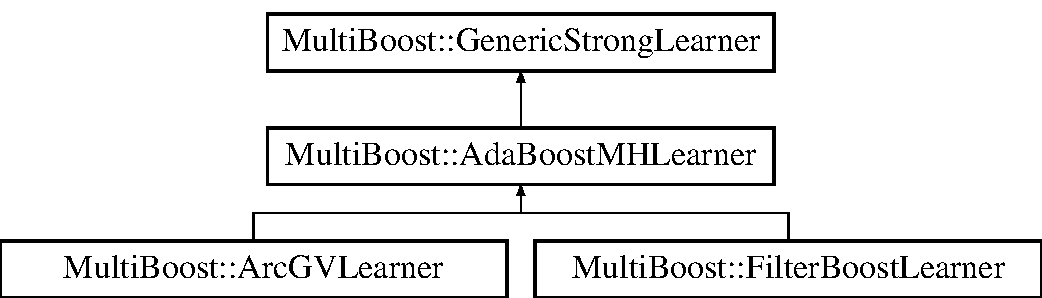
\includegraphics[height=3.000000cm]{classMultiBoost_1_1AdaBoostMHLearner}
\end{center}
\end{figure}
\subsection*{Public Member Functions}
\begin{DoxyCompactItemize}
\item 
\hyperlink{classMultiBoost_1_1AdaBoostMHLearner_a583ec3dfcb01bf1ae5270a8b60c50479}{Ada\-Boost\-M\-H\-Learner} ()
\item 
virtual void \hyperlink{classMultiBoost_1_1AdaBoostMHLearner_a1171d948bfa1875bf663993f067a8e8d}{run} (const \hyperlink{classnor__utils_1_1Args}{nor\-\_\-utils\-::\-Args} \&args)
\item 
void \hyperlink{classMultiBoost_1_1AdaBoostMHLearner_a6cc18ddef41bb0a8981e03c4e5b41be2}{run} (const \hyperlink{classnor__utils_1_1Args}{nor\-\_\-utils\-::\-Args} \&args, \hyperlink{classMultiBoost_1_1InputData}{Input\-Data} $\ast$p\-Training\-Data, const string base\-Learner\-Name, const int num\-Iterations, vector$<$ \hyperlink{classMultiBoost_1_1BaseLearner}{Base\-Learner} $\ast$ $>$ \&found\-Hypotheses)
\item 
virtual void \hyperlink{classMultiBoost_1_1AdaBoostMHLearner_ab2370f7d03a14d9cb67e130e3814a6f0}{classify} (const \hyperlink{classnor__utils_1_1Args}{nor\-\_\-utils\-::\-Args} \&args)
\item 
virtual void \hyperlink{classMultiBoost_1_1AdaBoostMHLearner_a234cd2586240f3a07dcbe5186babf8ad}{do\-Confusion\-Matrix} (const \hyperlink{classnor__utils_1_1Args}{nor\-\_\-utils\-::\-Args} \&args)
\item 
virtual void \hyperlink{classMultiBoost_1_1AdaBoostMHLearner_ab0067a96a9a7c2648cb0cfc8a97d8004}{do\-Posteriors} (const \hyperlink{classnor__utils_1_1Args}{nor\-\_\-utils\-::\-Args} \&args)
\item 
\hyperlink{Defaults_8h_a80184c4fd10ab70a1a17c5f97dcd1563}{Alpha\-Real} \hyperlink{classMultiBoost_1_1AdaBoostMHLearner_a909140ca1b8174c42695e57065b3c8b9}{update\-Weights} (\hyperlink{classMultiBoost_1_1InputData}{Input\-Data} $\ast$p\-Training\-Data, \hyperlink{classMultiBoost_1_1BaseLearner}{Base\-Learner} $\ast$p\-Weak\-Hypothesis)
\item 
\hyperlink{Defaults_8h_a80184c4fd10ab70a1a17c5f97dcd1563}{Alpha\-Real} \hyperlink{classMultiBoost_1_1AdaBoostMHLearner_a496a96f5c332bc11bd0c680a62964344}{update\-Weights} (\hyperlink{classMultiBoost_1_1OutputInfo}{Output\-Info} $\ast$p\-Out\-Info, \hyperlink{classMultiBoost_1_1InputData}{Input\-Data} $\ast$p\-Data, vector$<$ \hyperlink{classMultiBoost_1_1BaseLearner}{Base\-Learner} $\ast$ $>$ \&p\-Weak\-Hypothesis)
\item 
void \hyperlink{classMultiBoost_1_1AdaBoostMHLearner_a2bde373d5f80a4fd57b7de09e8ef327b}{print\-Output\-Info} (\hyperlink{classMultiBoost_1_1OutputInfo}{Output\-Info} $\ast$p\-Out\-Info, int t, \hyperlink{classMultiBoost_1_1InputData}{Input\-Data} $\ast$p\-Training\-Data, \hyperlink{classMultiBoost_1_1InputData}{Input\-Data} $\ast$p\-Test\-Data, \hyperlink{classMultiBoost_1_1BaseLearner}{Base\-Learner} $\ast$p\-Weak\-Hypothesis)
\item 
void \hyperlink{classMultiBoost_1_1AdaBoostMHLearner_aab49c681fb8c5eee29f346a46c2a5e29}{print\-Out\-Weights} (\hyperlink{classMultiBoost_1_1InputData}{Input\-Data} $\ast$p\-Data)
\end{DoxyCompactItemize}
\subsection*{Protected Member Functions}
\begin{DoxyCompactItemize}
\item 
void \hyperlink{classMultiBoost_1_1AdaBoostMHLearner_a45075e518fae57257fd9cfb8535060b1}{get\-Args} (const \hyperlink{classnor__utils_1_1Args}{nor\-\_\-utils\-::\-Args} \&args)
\item 
int \hyperlink{classMultiBoost_1_1AdaBoostMHLearner_af13c90ad8fc53b88d1f20e8d52ba0049}{resume\-Weak\-Learners} (\hyperlink{classMultiBoost_1_1InputData}{Input\-Data} $\ast$p\-Training\-Data)
\item 
void \hyperlink{classMultiBoost_1_1AdaBoostMHLearner_adf47da0cc22df7ebc55170dfea933203}{resume\-Process} (\hyperlink{classMultiBoost_1_1Serialization}{Serialization} \&ss, \hyperlink{classMultiBoost_1_1InputData}{Input\-Data} $\ast$p\-Training\-Data, \hyperlink{classMultiBoost_1_1InputData}{Input\-Data} $\ast$p\-Test\-Data, \hyperlink{classMultiBoost_1_1OutputInfo}{Output\-Info} $\ast$p\-Out\-Info)
\end{DoxyCompactItemize}
\subsection*{Protected Attributes}
\begin{DoxyCompactItemize}
\item 
\hypertarget{classMultiBoost_1_1AdaBoostMHLearner_a723596e1dcce33d594e1d9cb90c2e85f}{vector$<$ \hyperlink{classMultiBoost_1_1BaseLearner}{Base\-Learner} $\ast$ $>$ \hyperlink{classMultiBoost_1_1AdaBoostMHLearner_a723596e1dcce33d594e1d9cb90c2e85f}{\-\_\-found\-Hypotheses}}\label{classMultiBoost_1_1AdaBoostMHLearner_a723596e1dcce33d594e1d9cb90c2e85f}

\begin{DoxyCompactList}\small\item\em The list of the hypotheses found. \end{DoxyCompactList}\item 
\hypertarget{classMultiBoost_1_1AdaBoostMHLearner_adc925d29e89aec971adfe091307f36a7}{string \hyperlink{classMultiBoost_1_1AdaBoostMHLearner_adc925d29e89aec971adfe091307f36a7}{\-\_\-base\-Learner\-Name}}\label{classMultiBoost_1_1AdaBoostMHLearner_adc925d29e89aec971adfe091307f36a7}

\begin{DoxyCompactList}\small\item\em The name of the basic learner used by Ada\-Boost. \end{DoxyCompactList}\item 
\hypertarget{classMultiBoost_1_1AdaBoostMHLearner_aa6cefa59149ee78ab97cc159413c845f}{string \hyperlink{classMultiBoost_1_1AdaBoostMHLearner_aa6cefa59149ee78ab97cc159413c845f}{\-\_\-shyp\-File\-Name}}\label{classMultiBoost_1_1AdaBoostMHLearner_aa6cefa59149ee78ab97cc159413c845f}

\begin{DoxyCompactList}\small\item\em File name of the strong hypothesis. \end{DoxyCompactList}\item 
\hypertarget{classMultiBoost_1_1AdaBoostMHLearner_ade7af135ce1f11882e4ad2aae172121d}{bool {\bfseries \-\_\-is\-Shyp\-Compressed}}\label{classMultiBoost_1_1AdaBoostMHLearner_ade7af135ce1f11882e4ad2aae172121d}

\item 
\hypertarget{classMultiBoost_1_1AdaBoostMHLearner_a4e27fd8b14c4bfc9e2359b58b592aa16}{string {\bfseries \-\_\-train\-File\-Name}}\label{classMultiBoost_1_1AdaBoostMHLearner_a4e27fd8b14c4bfc9e2359b58b592aa16}

\item 
\hypertarget{classMultiBoost_1_1AdaBoostMHLearner_ad60eebad3afb84852f5bd8da314aa7fd}{string {\bfseries \-\_\-test\-File\-Name}}\label{classMultiBoost_1_1AdaBoostMHLearner_ad60eebad3afb84852f5bd8da314aa7fd}

\item 
\hypertarget{classMultiBoost_1_1AdaBoostMHLearner_a48db1d5b62055b631970d012f1e4656a}{int {\bfseries \-\_\-num\-Iterations}}\label{classMultiBoost_1_1AdaBoostMHLearner_a48db1d5b62055b631970d012f1e4656a}

\item 
\hypertarget{classMultiBoost_1_1AdaBoostMHLearner_a63d50b131c8e71523def6498213e0b50}{int \hyperlink{classMultiBoost_1_1AdaBoostMHLearner_a63d50b131c8e71523def6498213e0b50}{\-\_\-max\-Time}}\label{classMultiBoost_1_1AdaBoostMHLearner_a63d50b131c8e71523def6498213e0b50}

\begin{DoxyCompactList}\small\item\em Time limit for the whole processing. Default\-: no time limit (-\/1). \end{DoxyCompactList}\item 
\hypertarget{classMultiBoost_1_1AdaBoostMHLearner_a1dcf72e78dd6906d9500bda15efaaa5a}{\hyperlink{Defaults_8h_a80184c4fd10ab70a1a17c5f97dcd1563}{Alpha\-Real} \hyperlink{classMultiBoost_1_1AdaBoostMHLearner_a1dcf72e78dd6906d9500bda15efaaa5a}{\-\_\-theta}}\label{classMultiBoost_1_1AdaBoostMHLearner_a1dcf72e78dd6906d9500bda15efaaa5a}

\begin{DoxyCompactList}\small\item\em the value of theta. Default = 0. \end{DoxyCompactList}\item 
int \hyperlink{classMultiBoost_1_1AdaBoostMHLearner_a03f43502f6ffe9873dc383cc75cfa13d}{\-\_\-verbose}
\item 
\hypertarget{classMultiBoost_1_1AdaBoostMHLearner_ae2bd1ab538ad83c3f101945e36dc67b6}{const \hyperlink{Defaults_8h_a80184c4fd10ab70a1a17c5f97dcd1563}{Alpha\-Real} \hyperlink{classMultiBoost_1_1AdaBoostMHLearner_ae2bd1ab538ad83c3f101945e36dc67b6}{\-\_\-small\-Val}}\label{classMultiBoost_1_1AdaBoostMHLearner_ae2bd1ab538ad83c3f101945e36dc67b6}

\begin{DoxyCompactList}\small\item\em A small value, to solve numeric issues. \end{DoxyCompactList}\item 
string \hyperlink{classMultiBoost_1_1AdaBoostMHLearner_a2e6988a496276d32439f95970144c95c}{\-\_\-resume\-Shyp\-File\-Name}
\item 
\hypertarget{classMultiBoost_1_1AdaBoostMHLearner_aa122d670c3f294eee04620ef1baf15c7}{string \hyperlink{classMultiBoost_1_1AdaBoostMHLearner_aa122d670c3f294eee04620ef1baf15c7}{\-\_\-output\-Info\-File}}\label{classMultiBoost_1_1AdaBoostMHLearner_aa122d670c3f294eee04620ef1baf15c7}

\begin{DoxyCompactList}\small\item\em The filename of the step-\/by-\/step information file that will be updated. \end{DoxyCompactList}\item 
\hypertarget{classMultiBoost_1_1AdaBoostMHLearner_a8aae9fe5cd389062806ad713213eabc0}{string {\bfseries \-\_\-weight\-File}}\label{classMultiBoost_1_1AdaBoostMHLearner_a8aae9fe5cd389062806ad713213eabc0}

\item 
\hypertarget{classMultiBoost_1_1AdaBoostMHLearner_a48e5f2dfd1da6b43bcc0224fc341cc5b}{bool \hyperlink{classMultiBoost_1_1AdaBoostMHLearner_a48e5f2dfd1da6b43bcc0224fc341cc5b}{\-\_\-with\-Constant\-Learner}}\label{classMultiBoost_1_1AdaBoostMHLearner_a48e5f2dfd1da6b43bcc0224fc341cc5b}

\begin{DoxyCompactList}\small\item\em Check or not constant learner in each iteration. \end{DoxyCompactList}\item 
\hypertarget{classMultiBoost_1_1AdaBoostMHLearner_ae2f32a7b1285c02cdcb1c2d19a2d6b5a}{bool \hyperlink{classMultiBoost_1_1AdaBoostMHLearner_ae2f32a7b1285c02cdcb1c2d19a2d6b5a}{\-\_\-fast\-Resume\-Process}}\label{classMultiBoost_1_1AdaBoostMHLearner_ae2f32a7b1285c02cdcb1c2d19a2d6b5a}

\begin{DoxyCompactList}\small\item\em Fast resume process (true), it will calculate only the error rate of the last iteration. \end{DoxyCompactList}\item 
bool \hyperlink{classMultiBoost_1_1AdaBoostMHLearner_aec9596ab86f3071c4dc0acb3729227ee}{\-\_\-early\-Stopping}
\begin{DoxyCompactList}\small\item\em stop before \-\_\-num\-Iterations iterations if test\-Error does not improve (only with traintest) \end{DoxyCompactList}\item 
\hypertarget{classMultiBoost_1_1AdaBoostMHLearner_a504a1882f72446d399cafc9659f5cd8c}{int \hyperlink{classMultiBoost_1_1AdaBoostMHLearner_a504a1882f72446d399cafc9659f5cd8c}{\-\_\-early\-Stopping\-Min\-Iterations}}\label{classMultiBoost_1_1AdaBoostMHLearner_a504a1882f72446d399cafc9659f5cd8c}

\begin{DoxyCompactList}\small\item\em don't early stop before \-\_\-early\-Stopping\-Min\-Iterations iterations \end{DoxyCompactList}\item 
\hypertarget{classMultiBoost_1_1AdaBoostMHLearner_a78e937859e7dac27fa1cc50351e95437}{double \hyperlink{classMultiBoost_1_1AdaBoostMHLearner_a78e937859e7dac27fa1cc50351e95437}{\-\_\-early\-Stopping\-Smoothing\-Window\-Rate}}\label{classMultiBoost_1_1AdaBoostMHLearner_a78e937859e7dac27fa1cc50351e95437}

\begin{DoxyCompactList}\small\item\em test errors are averaged in the last \-\_\-early\-Stopping\-Smoothing\-Window\-Rate$\ast$\-T \end{DoxyCompactList}\item 
\hypertarget{classMultiBoost_1_1AdaBoostMHLearner_ab45304a1270a4f23ceda87c70a84cb45}{bool {\bfseries \-\_\-early\-Stopping\-Done}}\label{classMultiBoost_1_1AdaBoostMHLearner_ab45304a1270a4f23ceda87c70a84cb45}

\item 
\hypertarget{classMultiBoost_1_1AdaBoostMHLearner_aba5c79624c7628d5c1aed225dcaa0151}{string {\bfseries \-\_\-early\-Stopping\-Output\-Column}}\label{classMultiBoost_1_1AdaBoostMHLearner_aba5c79624c7628d5c1aed225dcaa0151}

\item 
\hypertarget{classMultiBoost_1_1AdaBoostMHLearner_acca83106fa1d58750d00dfdbfcc85d2d}{int \hyperlink{classMultiBoost_1_1AdaBoostMHLearner_acca83106fa1d58750d00dfdbfcc85d2d}{\-\_\-early\-Stopping\-Max\-Lookahead\-Rate}}\label{classMultiBoost_1_1AdaBoostMHLearner_acca83106fa1d58750d00dfdbfcc85d2d}

\begin{DoxyCompactList}\small\item\em if the minimum is reached at Tmin, \end{DoxyCompactList}\item 
\hypertarget{classMultiBoost_1_1AdaBoostMHLearner_af104d5111150afc00187df762a42defd}{int \hyperlink{classMultiBoost_1_1AdaBoostMHLearner_af104d5111150afc00187df762a42defd}{\-\_\-current\-Min\-T}}\label{classMultiBoost_1_1AdaBoostMHLearner_af104d5111150afc00187df762a42defd}

\begin{DoxyCompactList}\small\item\em the iteration where the smoothed error is minimal so far \end{DoxyCompactList}\item 
\hypertarget{classMultiBoost_1_1AdaBoostMHLearner_a23e89c84081e8591624afa3ba715b395}{\hyperlink{Defaults_8h_a80184c4fd10ab70a1a17c5f97dcd1563}{Alpha\-Real} {\bfseries sum\-Error\-Window}}\label{classMultiBoost_1_1AdaBoostMHLearner_a23e89c84081e8591624afa3ba715b395}

\item 
\hypertarget{classMultiBoost_1_1AdaBoostMHLearner_ace4d2f4d53fe8c55866520ecd271d26f}{int {\bfseries num\-Error\-Window}}\label{classMultiBoost_1_1AdaBoostMHLearner_ace4d2f4d53fe8c55866520ecd271d26f}

\item 
\hypertarget{classMultiBoost_1_1AdaBoostMHLearner_a3a30133d9df2444482d6c2995b572927}{\hyperlink{Defaults_8h_a80184c4fd10ab70a1a17c5f97dcd1563}{Alpha\-Real} {\bfseries current\-Min}}\label{classMultiBoost_1_1AdaBoostMHLearner_a3a30133d9df2444482d6c2995b572927}

\end{DoxyCompactItemize}


\subsection{Detailed Description}
The Ada\-Boost learner. This class performs the meta-\/learning by calling the weak learners and updating the weights. \begin{DoxyDate}{Date}
12/11/2005 
\end{DoxyDate}


Definition at line 63 of file Ada\-Boost\-M\-H\-Learner.\-h.



\subsection{Constructor \& Destructor Documentation}
\hypertarget{classMultiBoost_1_1AdaBoostMHLearner_a583ec3dfcb01bf1ae5270a8b60c50479}{\index{Multi\-Boost\-::\-Ada\-Boost\-M\-H\-Learner@{Multi\-Boost\-::\-Ada\-Boost\-M\-H\-Learner}!Ada\-Boost\-M\-H\-Learner@{Ada\-Boost\-M\-H\-Learner}}
\index{Ada\-Boost\-M\-H\-Learner@{Ada\-Boost\-M\-H\-Learner}!MultiBoost::AdaBoostMHLearner@{Multi\-Boost\-::\-Ada\-Boost\-M\-H\-Learner}}
\subsubsection[{Ada\-Boost\-M\-H\-Learner}]{\setlength{\rightskip}{0pt plus 5cm}Multi\-Boost\-::\-Ada\-Boost\-M\-H\-Learner\-::\-Ada\-Boost\-M\-H\-Learner (
\begin{DoxyParamCaption}
{}
\end{DoxyParamCaption}
)\hspace{0.3cm}{\ttfamily [inline]}}}\label{classMultiBoost_1_1AdaBoostMHLearner_a583ec3dfcb01bf1ae5270a8b60c50479}
The constructor. It initializes the variables and sets them using the information provided by the arguments passed. They are parsed using the helpers provided by class Args. \begin{DoxyDate}{Date}
13/11/2005 
\end{DoxyDate}


Definition at line 73 of file Ada\-Boost\-M\-H\-Learner.\-h.



\subsection{Member Function Documentation}
\hypertarget{classMultiBoost_1_1AdaBoostMHLearner_ab2370f7d03a14d9cb67e130e3814a6f0}{\index{Multi\-Boost\-::\-Ada\-Boost\-M\-H\-Learner@{Multi\-Boost\-::\-Ada\-Boost\-M\-H\-Learner}!classify@{classify}}
\index{classify@{classify}!MultiBoost::AdaBoostMHLearner@{Multi\-Boost\-::\-Ada\-Boost\-M\-H\-Learner}}
\subsubsection[{classify}]{\setlength{\rightskip}{0pt plus 5cm}void Multi\-Boost\-::\-Ada\-Boost\-M\-H\-Learner\-::classify (
\begin{DoxyParamCaption}
\item[{const {\bf nor\-\_\-utils\-::\-Args} \&}]{args}
\end{DoxyParamCaption}
)\hspace{0.3cm}{\ttfamily [virtual]}}}\label{classMultiBoost_1_1AdaBoostMHLearner_ab2370f7d03a14d9cb67e130e3814a6f0}
Performs the classification using the \hyperlink{classMultiBoost_1_1AdaBoostMHClassifier}{Ada\-Boost\-M\-H\-Classifier}. 
\begin{DoxyParams}{Parameters}
{\em args} & The arguments provided by the command line with all the options for classification. \\
\hline
\end{DoxyParams}


Implements \hyperlink{classMultiBoost_1_1GenericStrongLearner_ad4b2a6aeca5917c841c5747f0bf81e90}{Multi\-Boost\-::\-Generic\-Strong\-Learner}.



Definition at line 416 of file Ada\-Boost\-M\-H\-Learner.\-cpp.

\hypertarget{classMultiBoost_1_1AdaBoostMHLearner_a234cd2586240f3a07dcbe5186babf8ad}{\index{Multi\-Boost\-::\-Ada\-Boost\-M\-H\-Learner@{Multi\-Boost\-::\-Ada\-Boost\-M\-H\-Learner}!do\-Confusion\-Matrix@{do\-Confusion\-Matrix}}
\index{do\-Confusion\-Matrix@{do\-Confusion\-Matrix}!MultiBoost::AdaBoostMHLearner@{Multi\-Boost\-::\-Ada\-Boost\-M\-H\-Learner}}
\subsubsection[{do\-Confusion\-Matrix}]{\setlength{\rightskip}{0pt plus 5cm}void Multi\-Boost\-::\-Ada\-Boost\-M\-H\-Learner\-::do\-Confusion\-Matrix (
\begin{DoxyParamCaption}
\item[{const {\bf nor\-\_\-utils\-::\-Args} \&}]{args}
\end{DoxyParamCaption}
)\hspace{0.3cm}{\ttfamily [virtual]}}}\label{classMultiBoost_1_1AdaBoostMHLearner_a234cd2586240f3a07dcbe5186babf8ad}
Print to stdout (or to file) a confusion matrix. 
\begin{DoxyParams}{Parameters}
{\em args} & The arguments provided by the command line. \\
\hline
\end{DoxyParams}
\begin{DoxyDate}{Date}
20/3/2006 
\end{DoxyDate}


Implements \hyperlink{classMultiBoost_1_1GenericStrongLearner_a3b9a92fd37fe14cdc56c1b216b4d6889}{Multi\-Boost\-::\-Generic\-Strong\-Learner}.



Definition at line 434 of file Ada\-Boost\-M\-H\-Learner.\-cpp.

\hypertarget{classMultiBoost_1_1AdaBoostMHLearner_ab0067a96a9a7c2648cb0cfc8a97d8004}{\index{Multi\-Boost\-::\-Ada\-Boost\-M\-H\-Learner@{Multi\-Boost\-::\-Ada\-Boost\-M\-H\-Learner}!do\-Posteriors@{do\-Posteriors}}
\index{do\-Posteriors@{do\-Posteriors}!MultiBoost::AdaBoostMHLearner@{Multi\-Boost\-::\-Ada\-Boost\-M\-H\-Learner}}
\subsubsection[{do\-Posteriors}]{\setlength{\rightskip}{0pt plus 5cm}void Multi\-Boost\-::\-Ada\-Boost\-M\-H\-Learner\-::do\-Posteriors (
\begin{DoxyParamCaption}
\item[{const {\bf nor\-\_\-utils\-::\-Args} \&}]{args}
\end{DoxyParamCaption}
)\hspace{0.3cm}{\ttfamily [virtual]}}}\label{classMultiBoost_1_1AdaBoostMHLearner_ab0067a96a9a7c2648cb0cfc8a97d8004}
Output the outcome of the strong learner for each class. Strictly speaking these are (currently) not posteriors, as the sum of these values is not one. 
\begin{DoxyParams}{Parameters}
{\em args} & The arguments provided by the command line. \\
\hline
\end{DoxyParams}


Implements \hyperlink{classMultiBoost_1_1GenericStrongLearner_adf92c9fd773dab4e960dee744adf3654}{Multi\-Boost\-::\-Generic\-Strong\-Learner}.



Definition at line 460 of file Ada\-Boost\-M\-H\-Learner.\-cpp.

\hypertarget{classMultiBoost_1_1AdaBoostMHLearner_a45075e518fae57257fd9cfb8535060b1}{\index{Multi\-Boost\-::\-Ada\-Boost\-M\-H\-Learner@{Multi\-Boost\-::\-Ada\-Boost\-M\-H\-Learner}!get\-Args@{get\-Args}}
\index{get\-Args@{get\-Args}!MultiBoost::AdaBoostMHLearner@{Multi\-Boost\-::\-Ada\-Boost\-M\-H\-Learner}}
\subsubsection[{get\-Args}]{\setlength{\rightskip}{0pt plus 5cm}void Multi\-Boost\-::\-Ada\-Boost\-M\-H\-Learner\-::get\-Args (
\begin{DoxyParamCaption}
\item[{const {\bf nor\-\_\-utils\-::\-Args} \&}]{args}
\end{DoxyParamCaption}
)\hspace{0.3cm}{\ttfamily [protected]}}}\label{classMultiBoost_1_1AdaBoostMHLearner_a45075e518fae57257fd9cfb8535060b1}
Get the needed parameters (for the strong learner) from the argumens. 
\begin{DoxyParams}{Parameters}
{\em The} & arguments provided by the command line. \\
\hline
\end{DoxyParams}


Definition at line 55 of file Ada\-Boost\-M\-H\-Learner.\-cpp.

\hypertarget{classMultiBoost_1_1AdaBoostMHLearner_a2bde373d5f80a4fd57b7de09e8ef327b}{\index{Multi\-Boost\-::\-Ada\-Boost\-M\-H\-Learner@{Multi\-Boost\-::\-Ada\-Boost\-M\-H\-Learner}!print\-Output\-Info@{print\-Output\-Info}}
\index{print\-Output\-Info@{print\-Output\-Info}!MultiBoost::AdaBoostMHLearner@{Multi\-Boost\-::\-Ada\-Boost\-M\-H\-Learner}}
\subsubsection[{print\-Output\-Info}]{\setlength{\rightskip}{0pt plus 5cm}void Multi\-Boost\-::\-Ada\-Boost\-M\-H\-Learner\-::print\-Output\-Info (
\begin{DoxyParamCaption}
\item[{{\bf Output\-Info} $\ast$}]{p\-Out\-Info, }
\item[{int}]{t, }
\item[{{\bf Input\-Data} $\ast$}]{p\-Training\-Data, }
\item[{{\bf Input\-Data} $\ast$}]{p\-Test\-Data, }
\item[{{\bf Base\-Learner} $\ast$}]{p\-Weak\-Hypothesis}
\end{DoxyParamCaption}
)}}\label{classMultiBoost_1_1AdaBoostMHLearner_a2bde373d5f80a4fd57b7de09e8ef327b}
Print output information if option --outputinfo is specified. Called from run and resume\-Process \begin{DoxySeeAlso}{See Also}
\hyperlink{classMultiBoost_1_1AdaBoostMHLearner_adf47da0cc22df7ebc55170dfea933203}{resume\-Process} 

\hyperlink{classMultiBoost_1_1AdaBoostMHLearner_a1171d948bfa1875bf663993f067a8e8d}{run} 
\end{DoxySeeAlso}
\begin{DoxyDate}{Date}
21/04/2007 
\end{DoxyDate}


Definition at line 836 of file Ada\-Boost\-M\-H\-Learner.\-cpp.

\hypertarget{classMultiBoost_1_1AdaBoostMHLearner_aab49c681fb8c5eee29f346a46c2a5e29}{\index{Multi\-Boost\-::\-Ada\-Boost\-M\-H\-Learner@{Multi\-Boost\-::\-Ada\-Boost\-M\-H\-Learner}!print\-Out\-Weights@{print\-Out\-Weights}}
\index{print\-Out\-Weights@{print\-Out\-Weights}!MultiBoost::AdaBoostMHLearner@{Multi\-Boost\-::\-Ada\-Boost\-M\-H\-Learner}}
\subsubsection[{print\-Out\-Weights}]{\setlength{\rightskip}{0pt plus 5cm}void Multi\-Boost\-::\-Ada\-Boost\-M\-H\-Learner\-::print\-Out\-Weights (
\begin{DoxyParamCaption}
\item[{{\bf Input\-Data} $\ast$}]{p\-Data}
\end{DoxyParamCaption}
)}}\label{classMultiBoost_1_1AdaBoostMHLearner_aab49c681fb8c5eee29f346a46c2a5e29}
Print out the weights of the instances at the end of the learning process if output file is given. \begin{DoxySeeAlso}{See Also}
\hyperlink{classMultiBoost_1_1AdaBoostMHLearner_a1171d948bfa1875bf663993f067a8e8d}{run} 
\end{DoxySeeAlso}
\begin{DoxyDate}{Date}
29/04/2010 
\end{DoxyDate}


Definition at line 857 of file Ada\-Boost\-M\-H\-Learner.\-cpp.

\hypertarget{classMultiBoost_1_1AdaBoostMHLearner_adf47da0cc22df7ebc55170dfea933203}{\index{Multi\-Boost\-::\-Ada\-Boost\-M\-H\-Learner@{Multi\-Boost\-::\-Ada\-Boost\-M\-H\-Learner}!resume\-Process@{resume\-Process}}
\index{resume\-Process@{resume\-Process}!MultiBoost::AdaBoostMHLearner@{Multi\-Boost\-::\-Ada\-Boost\-M\-H\-Learner}}
\subsubsection[{resume\-Process}]{\setlength{\rightskip}{0pt plus 5cm}void Multi\-Boost\-::\-Ada\-Boost\-M\-H\-Learner\-::resume\-Process (
\begin{DoxyParamCaption}
\item[{{\bf Serialization} \&}]{ss, }
\item[{{\bf Input\-Data} $\ast$}]{p\-Training\-Data, }
\item[{{\bf Input\-Data} $\ast$}]{p\-Test\-Data, }
\item[{{\bf Output\-Info} $\ast$}]{p\-Out\-Info}
\end{DoxyParamCaption}
)\hspace{0.3cm}{\ttfamily [protected]}}}\label{classMultiBoost_1_1AdaBoostMHLearner_adf47da0cc22df7ebc55170dfea933203}
Resume the training using the features in \-\_\-resume\-Shyp\-File\-Name if the option -\/resume has been specified. \begin{DoxyDate}{Date}
21/12/2005 
\end{DoxyDate}


Definition at line 709 of file Ada\-Boost\-M\-H\-Learner.\-cpp.

\hypertarget{classMultiBoost_1_1AdaBoostMHLearner_af13c90ad8fc53b88d1f20e8d52ba0049}{\index{Multi\-Boost\-::\-Ada\-Boost\-M\-H\-Learner@{Multi\-Boost\-::\-Ada\-Boost\-M\-H\-Learner}!resume\-Weak\-Learners@{resume\-Weak\-Learners}}
\index{resume\-Weak\-Learners@{resume\-Weak\-Learners}!MultiBoost::AdaBoostMHLearner@{Multi\-Boost\-::\-Ada\-Boost\-M\-H\-Learner}}
\subsubsection[{resume\-Weak\-Learners}]{\setlength{\rightskip}{0pt plus 5cm}int Multi\-Boost\-::\-Ada\-Boost\-M\-H\-Learner\-::resume\-Weak\-Learners (
\begin{DoxyParamCaption}
\item[{{\bf Input\-Data} $\ast$}]{p\-Training\-Data}
\end{DoxyParamCaption}
)\hspace{0.3cm}{\ttfamily [protected]}}}\label{classMultiBoost_1_1AdaBoostMHLearner_af13c90ad8fc53b88d1f20e8d52ba0049}
Resume the weak learner list. \begin{DoxyReturn}{Returns}
The current iteration number. 0 if not -\/resume option has been called 
\end{DoxyReturn}

\begin{DoxyParams}{Parameters}
{\em p\-Training\-Data} & The pointer to the training data, needed for class\-Map, enum\-Maps. \\
\hline
\end{DoxyParams}
\begin{DoxyDate}{Date}
21/12/2005 
\end{DoxyDate}
\begin{DoxySeeAlso}{See Also}
\hyperlink{classMultiBoost_1_1AdaBoostMHLearner_adf47da0cc22df7ebc55170dfea933203}{resume\-Process} 
\end{DoxySeeAlso}
\begin{DoxyRemark}{Remarks}
resume\-Process must be called too! 
\end{DoxyRemark}


Definition at line 686 of file Ada\-Boost\-M\-H\-Learner.\-cpp.

\hypertarget{classMultiBoost_1_1AdaBoostMHLearner_a1171d948bfa1875bf663993f067a8e8d}{\index{Multi\-Boost\-::\-Ada\-Boost\-M\-H\-Learner@{Multi\-Boost\-::\-Ada\-Boost\-M\-H\-Learner}!run@{run}}
\index{run@{run}!MultiBoost::AdaBoostMHLearner@{Multi\-Boost\-::\-Ada\-Boost\-M\-H\-Learner}}
\subsubsection[{run}]{\setlength{\rightskip}{0pt plus 5cm}void Multi\-Boost\-::\-Ada\-Boost\-M\-H\-Learner\-::run (
\begin{DoxyParamCaption}
\item[{const {\bf nor\-\_\-utils\-::\-Args} \&}]{args}
\end{DoxyParamCaption}
)\hspace{0.3cm}{\ttfamily [virtual]}}}\label{classMultiBoost_1_1AdaBoostMHLearner_a1171d948bfa1875bf663993f067a8e8d}
Start the learning process. 
\begin{DoxyParams}{Parameters}
{\em args} & The arguments provided by the command line with all the options for training. \\
\hline
\end{DoxyParams}
\begin{DoxySeeAlso}{See Also}
\hyperlink{classMultiBoost_1_1OutputInfo}{Output\-Info} 
\end{DoxySeeAlso}
\begin{DoxyDate}{Date}
10/11/2005 
\end{DoxyDate}


Implements \hyperlink{classMultiBoost_1_1GenericStrongLearner_a77c75c5cbc867c191b327e5a04e9f147}{Multi\-Boost\-::\-Generic\-Strong\-Learner}.



Reimplemented in \hyperlink{classMultiBoost_1_1FilterBoostLearner_a3209ce71f29e342c84142d9623583109}{Multi\-Boost\-::\-Filter\-Boost\-Learner}, and \hyperlink{classMultiBoost_1_1ArcGVLearner_ad2e5b9873d3c752307d9639ff53ee86a}{Multi\-Boost\-::\-Arc\-G\-V\-Learner}.



Definition at line 154 of file Ada\-Boost\-M\-H\-Learner.\-cpp.

\hypertarget{classMultiBoost_1_1AdaBoostMHLearner_a6cc18ddef41bb0a8981e03c4e5b41be2}{\index{Multi\-Boost\-::\-Ada\-Boost\-M\-H\-Learner@{Multi\-Boost\-::\-Ada\-Boost\-M\-H\-Learner}!run@{run}}
\index{run@{run}!MultiBoost::AdaBoostMHLearner@{Multi\-Boost\-::\-Ada\-Boost\-M\-H\-Learner}}
\subsubsection[{run}]{\setlength{\rightskip}{0pt plus 5cm}void Multi\-Boost\-::\-Ada\-Boost\-M\-H\-Learner\-::run (
\begin{DoxyParamCaption}
\item[{const {\bf nor\-\_\-utils\-::\-Args} \&}]{args, }
\item[{{\bf Input\-Data} $\ast$}]{p\-Training\-Data, }
\item[{const string}]{base\-Learner\-Name, }
\item[{const int}]{num\-Iterations, }
\item[{vector$<$ {\bf Base\-Learner} $\ast$ $>$ \&}]{found\-Hypotheses}
\end{DoxyParamCaption}
)}}\label{classMultiBoost_1_1AdaBoostMHLearner_a6cc18ddef41bb0a8981e03c4e5b41be2}
For Soft\-Cascade 
\begin{DoxyParams}{Parameters}
{\em args} & The arguments provided by the command line with all the options for training. \\
\hline
\end{DoxyParams}
\begin{DoxySeeAlso}{See Also}
\hyperlink{classMultiBoost_1_1OutputInfo}{Output\-Info} 
\end{DoxySeeAlso}
\begin{DoxyDate}{Date}
10/11/2005 
\end{DoxyDate}


Definition at line 898 of file Ada\-Boost\-M\-H\-Learner.\-cpp.

\hypertarget{classMultiBoost_1_1AdaBoostMHLearner_a909140ca1b8174c42695e57065b3c8b9}{\index{Multi\-Boost\-::\-Ada\-Boost\-M\-H\-Learner@{Multi\-Boost\-::\-Ada\-Boost\-M\-H\-Learner}!update\-Weights@{update\-Weights}}
\index{update\-Weights@{update\-Weights}!MultiBoost::AdaBoostMHLearner@{Multi\-Boost\-::\-Ada\-Boost\-M\-H\-Learner}}
\subsubsection[{update\-Weights}]{\setlength{\rightskip}{0pt plus 5cm}{\bf Alpha\-Real} Multi\-Boost\-::\-Ada\-Boost\-M\-H\-Learner\-::update\-Weights (
\begin{DoxyParamCaption}
\item[{{\bf Input\-Data} $\ast$}]{p\-Training\-Data, }
\item[{{\bf Base\-Learner} $\ast$}]{p\-Weak\-Hypothesis}
\end{DoxyParamCaption}
)}}\label{classMultiBoost_1_1AdaBoostMHLearner_a909140ca1b8174c42695e57065b3c8b9}
Updates the weights of the examples. The re-\/weighting of $w$ (the weight vector over all the examples and classes) is done using the following formula \[ w^{(t+1)}_{i, \ell}= \frac{ w^{(t)}_{i, \ell} \exp \left( -\alpha^{(t)} h_\ell^{(t)}(x_i) y_{i, \ell} \right) }{ Z^{(t)} } \] where {\itshape Z} is a normalization factor, and it is defined as \[ Z^{(t)} = \sum_{j=1}^n \sum_{\ell=1}^k w^{(t)}_{j, \ell} \exp \left( -\alpha^{(t)} h_\ell^{(t)}(x_j) y_{j, \ell} \right) \] where $n$ is the number of examples, $k$ the number of classes, $\alpha$ is the confidence in the weak classifier, $h_\ell(x_i)$ is the classification of example $x_i$ for class $\ell$ with the classifier found at the current iteration (see \hyperlink{classMultiBoost_1_1BaseLearner_af8bccd75a88d572a24ea337abcaa00f0}{Base\-Learner\-::classify()}), and $y_i$ is the binary label of that example, defined in Input\-Data\-::get\-Binary\-Class(). 
\begin{DoxyParams}{Parameters}
{\em p\-Training\-Data} & The pointer to the training data. \\
\hline
{\em p\-Weak\-Hypothesis} & The current weak hypothesis. \\
\hline
\end{DoxyParams}
\begin{DoxyReturn}{Returns}
The value of the edge. It will be used to see if the algorithm can continue with learning. 
\end{DoxyReturn}
\begin{DoxyDate}{Date}
16/11/2005 
\end{DoxyDate}


Definition at line 584 of file Ada\-Boost\-M\-H\-Learner.\-cpp.

\hypertarget{classMultiBoost_1_1AdaBoostMHLearner_a496a96f5c332bc11bd0c680a62964344}{\index{Multi\-Boost\-::\-Ada\-Boost\-M\-H\-Learner@{Multi\-Boost\-::\-Ada\-Boost\-M\-H\-Learner}!update\-Weights@{update\-Weights}}
\index{update\-Weights@{update\-Weights}!MultiBoost::AdaBoostMHLearner@{Multi\-Boost\-::\-Ada\-Boost\-M\-H\-Learner}}
\subsubsection[{update\-Weights}]{\setlength{\rightskip}{0pt plus 5cm}{\bf Alpha\-Real} Multi\-Boost\-::\-Ada\-Boost\-M\-H\-Learner\-::update\-Weights (
\begin{DoxyParamCaption}
\item[{{\bf Output\-Info} $\ast$}]{p\-Out\-Info, }
\item[{{\bf Input\-Data} $\ast$}]{p\-Data, }
\item[{vector$<$ {\bf Base\-Learner} $\ast$ $>$ \&}]{p\-Weak\-Hypothesis}
\end{DoxyParamCaption}
)}}\label{classMultiBoost_1_1AdaBoostMHLearner_a496a96f5c332bc11bd0c680a62964344}
Updates the weights of the examples. If the slowresumeprocess is on, we do not calculate the weights in every iteration, but we calculate the re-\/weighting based on the exponential margins. Let's assume that it is given a strong learner $\f^{(t)}(\bx)\$f after t iteration. Then the weights of the $+1 

Definition at line 482 of file Ada\-Boost\-M\-H\-Learner.\-cpp.



\subsection{Member Data Documentation}
\hypertarget{classMultiBoost_1_1AdaBoostMHLearner_aec9596ab86f3071c4dc0acb3729227ee}{\index{Multi\-Boost\-::\-Ada\-Boost\-M\-H\-Learner@{Multi\-Boost\-::\-Ada\-Boost\-M\-H\-Learner}!\-\_\-early\-Stopping@{\-\_\-early\-Stopping}}
\index{\-\_\-early\-Stopping@{\-\_\-early\-Stopping}!MultiBoost::AdaBoostMHLearner@{Multi\-Boost\-::\-Ada\-Boost\-M\-H\-Learner}}
\subsubsection[{\-\_\-early\-Stopping}]{\setlength{\rightskip}{0pt plus 5cm}bool Multi\-Boost\-::\-Ada\-Boost\-M\-H\-Learner\-::\-\_\-early\-Stopping\hspace{0.3cm}{\ttfamily [protected]}}}\label{classMultiBoost_1_1AdaBoostMHLearner_aec9596ab86f3071c4dc0acb3729227ee}


stop before \-\_\-num\-Iterations iterations if test\-Error does not improve (only with traintest) 

In traintest mode we may stop before \-\_\-num\-Iterations iterations or \-\_\-max\-Time time. In iteration T, if T $>$ \-\_\-early\-Stopping\-Min\-Iterations, we compute the average test error in the last \-\_\-early\-Stopping\-Smoothing\-Window\-Rate$\ast$ Titerations. Let the current minimum of this smoothed error be taken at Tmin. We stop if T $>$ \-\_\-early\-Stopping\-Max\-Lookahead\-Rate$\ast$\-Tmin. 

Definition at line 247 of file Ada\-Boost\-M\-H\-Learner.\-h.

\hypertarget{classMultiBoost_1_1AdaBoostMHLearner_a2e6988a496276d32439f95970144c95c}{\index{Multi\-Boost\-::\-Ada\-Boost\-M\-H\-Learner@{Multi\-Boost\-::\-Ada\-Boost\-M\-H\-Learner}!\-\_\-resume\-Shyp\-File\-Name@{\-\_\-resume\-Shyp\-File\-Name}}
\index{\-\_\-resume\-Shyp\-File\-Name@{\-\_\-resume\-Shyp\-File\-Name}!MultiBoost::AdaBoostMHLearner@{Multi\-Boost\-::\-Ada\-Boost\-M\-H\-Learner}}
\subsubsection[{\-\_\-resume\-Shyp\-File\-Name}]{\setlength{\rightskip}{0pt plus 5cm}string Multi\-Boost\-::\-Ada\-Boost\-M\-H\-Learner\-::\-\_\-resume\-Shyp\-File\-Name\hspace{0.3cm}{\ttfamily [protected]}}}\label{classMultiBoost_1_1AdaBoostMHLearner_a2e6988a496276d32439f95970144c95c}
If resume is set, this will hold the strong hypothesis file to load in order to continue with the training process. 

Definition at line 234 of file Ada\-Boost\-M\-H\-Learner.\-h.

\hypertarget{classMultiBoost_1_1AdaBoostMHLearner_a03f43502f6ffe9873dc383cc75cfa13d}{\index{Multi\-Boost\-::\-Ada\-Boost\-M\-H\-Learner@{Multi\-Boost\-::\-Ada\-Boost\-M\-H\-Learner}!\-\_\-verbose@{\-\_\-verbose}}
\index{\-\_\-verbose@{\-\_\-verbose}!MultiBoost::AdaBoostMHLearner@{Multi\-Boost\-::\-Ada\-Boost\-M\-H\-Learner}}
\subsubsection[{\-\_\-verbose}]{\setlength{\rightskip}{0pt plus 5cm}int Multi\-Boost\-::\-Ada\-Boost\-M\-H\-Learner\-::\-\_\-verbose\hspace{0.3cm}{\ttfamily [protected]}}}\label{classMultiBoost_1_1AdaBoostMHLearner_a03f43502f6ffe9873dc383cc75cfa13d}
Verbose level. There are three levels of verbosity\-:
\begin{DoxyItemize}
\item 0 = no messages
\item 1 = basic messages
\item 2 = show all messages 
\end{DoxyItemize}

Definition at line 227 of file Ada\-Boost\-M\-H\-Learner.\-h.



The documentation for this class was generated from the following files\-:\begin{DoxyCompactItemize}
\item 
C\-:/\-Users/fradav/\-Documents/\-Dev/\-C++/\-Multiboost/\-Sources/src/\-Strong\-Learners/\hyperlink{AdaBoostMHLearner_8h}{Ada\-Boost\-M\-H\-Learner.\-h}\item 
C\-:/\-Users/fradav/\-Documents/\-Dev/\-C++/\-Multiboost/\-Sources/src/\-Strong\-Learners/Ada\-Boost\-M\-H\-Learner.\-cpp\end{DoxyCompactItemize}

\hypertarget{classMultiBoost_1_1AdaLineLearner}{\section{Multi\-Boost\-:\-:Ada\-Line\-Learner Class Reference}
\label{classMultiBoost_1_1AdaLineLearner}\index{Multi\-Boost\-::\-Ada\-Line\-Learner@{Multi\-Boost\-::\-Ada\-Line\-Learner}}
}
Inheritance diagram for Multi\-Boost\-:\-:Ada\-Line\-Learner\-:\begin{figure}[H]
\begin{center}
\leavevmode
\includegraphics[height=4.000000cm]{classMultiBoost_1_1AdaLineLearner}
\end{center}
\end{figure}
\subsection*{Public Member Functions}
\begin{DoxyCompactItemize}
\item 
\hyperlink{classMultiBoost_1_1AdaLineLearner_ac13de8e5e86032b6d9e58eae860e4b8b}{Ada\-Line\-Learner} ()
\item 
virtual \hyperlink{classMultiBoost_1_1AdaLineLearner_adb36b069fcaede6a71d442151b1eb716}{$\sim$\-Ada\-Line\-Learner} ()
\item 
virtual void \hyperlink{classMultiBoost_1_1AdaLineLearner_a6c8f143382449c333995c33539bbff04}{declare\-Arguments} (\hyperlink{classnor__utils_1_1Args}{nor\-\_\-utils\-::\-Args} \&args)
\item 
virtual void \hyperlink{classMultiBoost_1_1AdaLineLearner_a4af94dbbbc29009456ef3e80e104f333}{init\-Learning\-Options} (const \hyperlink{classnor__utils_1_1Args}{nor\-\_\-utils\-::\-Args} \&args)
\item 
virtual void \hyperlink{classMultiBoost_1_1AdaLineLearner_a4b96e7dce0bb66b4dbe48caef6582699}{sub\-Copy\-State} (\hyperlink{classMultiBoost_1_1BaseLearner}{Base\-Learner} $\ast$p\-Base\-Learner)
\item 
virtual \hyperlink{classMultiBoost_1_1BaseLearner}{Base\-Learner} $\ast$ \hyperlink{classMultiBoost_1_1AdaLineLearner_a440d8ba8ddb784db3caa562813c5b293}{sub\-Create} ()
\item 
virtual \hyperlink{Defaults_8h_a80184c4fd10ab70a1a17c5f97dcd1563}{Alpha\-Real} \hyperlink{classMultiBoost_1_1AdaLineLearner_aaf0781525559a349d16b8f6cb8606fcf}{run} ()
\item 
virtual void \hyperlink{classMultiBoost_1_1AdaLineLearner_a7846d9abaa274ed08c6610a6314a2333}{init\-Learning} ()
\item 
virtual \hyperlink{Defaults_8h_a80184c4fd10ab70a1a17c5f97dcd1563}{Alpha\-Real} \hyperlink{classMultiBoost_1_1AdaLineLearner_a55fc3a35c4ef3374f06c1597122f203d}{finish\-Learning} ()
\item 
virtual \hyperlink{Defaults_8h_a80184c4fd10ab70a1a17c5f97dcd1563}{Alpha\-Real} \hyperlink{classMultiBoost_1_1AdaLineLearner_a5ce3ad08d70d156c8b72cd5c8990979d}{update} (int idx)
\end{DoxyCompactItemize}

\hypertarget{classMultiBoost_1_1ArffParser}{\section{Multi\-Boost\-:\-:Arff\-Parser Class Reference}
\label{classMultiBoost_1_1ArffParser}\index{Multi\-Boost\-::\-Arff\-Parser@{Multi\-Boost\-::\-Arff\-Parser}}
}
Inheritance diagram for Multi\-Boost\-:\-:Arff\-Parser\-:\begin{figure}[H]
\begin{center}
\leavevmode
\includegraphics[height=3.000000cm]{classMultiBoost_1_1ArffParser}
\end{center}
\end{figure}
\subsection*{Public Member Functions}
\begin{DoxyCompactItemize}
\item 
\hyperlink{classMultiBoost_1_1ArffParser_a0662914fbd497ca015a9f1b4d89b6cd0}{Arff\-Parser} (const string \&file\-Name, const string \&header\-File\-Name)
\item 
virtual void \hyperlink{classMultiBoost_1_1ArffParser_a1ede5df98cbce136f1e554dbaf974a4f}{read\-Data} (vector$<$ \hyperlink{classMultiBoost_1_1Example}{Example} $>$ \&examples, \hyperlink{classMultiBoost_1_1NameMap}{Name\-Map} \&class\-Map, vector$<$ \hyperlink{classMultiBoost_1_1NameMap}{Name\-Map} $>$ \&enum\-Maps, \hyperlink{classMultiBoost_1_1NameMap}{Name\-Map} \&attribute\-Name\-Map, vector$<$ Raw\-Data\-::e\-Attribute\-Type $>$ \&attribute\-Types)
\item 
virtual int \hyperlink{classMultiBoost_1_1ArffParser_aa2921ea554b3b8fd14aa893d7ab0eedd}{get\-Num\-Attributes} () const 
\end{DoxyCompactItemize}
\subsection*{Protected Types}
\begin{DoxyCompactItemize}
\item 
enum {\bfseries e\-Token\-Type} \{ \\*
{\bfseries T\-T\-\_\-\-E\-O\-F}, 
{\bfseries T\-T\-\_\-\-C\-O\-M\-M\-E\-N\-T}, 
{\bfseries T\-T\-\_\-\-R\-E\-L\-A\-T\-I\-O\-N}, 
{\bfseries T\-T\-\_\-\-A\-T\-T\-R\-I\-B\-U\-T\-E}, 
\\*
{\bfseries T\-T\-\_\-\-D\-A\-T\-A}, 
{\bfseries T\-T\-\_\-\-U\-N\-K\-N\-O\-W\-N}
 \}
\end{DoxyCompactItemize}
\subsection*{Protected Member Functions}
\begin{DoxyCompactItemize}
\item 
void \hyperlink{classMultiBoost_1_1ArffParser_ab399500474366a998ceb56b49cd113eb}{read\-Header} (ifstream \&in, \hyperlink{classMultiBoost_1_1NameMap}{Name\-Map} \&class\-Map, vector$<$ \hyperlink{classMultiBoost_1_1NameMap}{Name\-Map} $>$ \&enum\-Maps, \hyperlink{classMultiBoost_1_1NameMap}{Name\-Map} \&attribute\-Name\-Map, vector$<$ Raw\-Data\-::e\-Attribute\-Type $>$ \&attribute\-Types)
\item 
void \hyperlink{classMultiBoost_1_1ArffParser_a80e003a25ae5b4201f0fbe490b396c25}{read\-Data} (ifstream \&in, vector$<$ \hyperlink{classMultiBoost_1_1Example}{Example} $>$ \&examples, \hyperlink{classMultiBoost_1_1NameMap}{Name\-Map} \&class\-Map, vector$<$ \hyperlink{classMultiBoost_1_1NameMap}{Name\-Map} $>$ \&enum\-Maps, const vector$<$ Raw\-Data\-::e\-Attribute\-Type $>$ \&attribute\-Types)
\item 
\hypertarget{classMultiBoost_1_1ArffParser_a73825cf1ad7c4dccebf7f0cc46428389}{string {\bfseries read\-Name} (ifstream \&in)}\label{classMultiBoost_1_1ArffParser_a73825cf1ad7c4dccebf7f0cc46428389}

\item 
\hypertarget{classMultiBoost_1_1ArffParser_a44a540ac1a0904fb75d38e59aa28aa4f}{void {\bfseries read\-Dense\-Values} (ifstream \&in, vector$<$ \hyperlink{Defaults_8h_a3a11cfe6a5d469d921716ca6291e934f}{Feature\-Real} $>$ \&values, vector$<$ \hyperlink{classMultiBoost_1_1NameMap}{Name\-Map} $>$ \&enum\-Maps, const vector$<$ Raw\-Data\-::e\-Attribute\-Type $>$ \&attribute\-Types)}\label{classMultiBoost_1_1ArffParser_a44a540ac1a0904fb75d38e59aa28aa4f}

\item 
\hypertarget{classMultiBoost_1_1ArffParser_a885ffe32985c6549d15ea6fb8a453e9b}{void {\bfseries read\-Sparse\-Values} (istringstream \&ss, vector$<$ \hyperlink{Defaults_8h_a3a11cfe6a5d469d921716ca6291e934f}{Feature\-Real} $>$ \&values, vector$<$ int $>$ \&idxs, map$<$ int, int $>$ \&idxmap, vector$<$ \hyperlink{classMultiBoost_1_1NameMap}{Name\-Map} $>$ \&enum\-Maps, const vector$<$ Raw\-Data\-::e\-Attribute\-Type $>$ \&attribute\-Types)}\label{classMultiBoost_1_1ArffParser_a885ffe32985c6549d15ea6fb8a453e9b}

\item 
void \hyperlink{classMultiBoost_1_1ArffParser_a82dc32253c2a46ac911e1d711135e6a4}{read\-Simple\-Labels} (istringstream \&ss, vector$<$ \hyperlink{structMultiBoost_1_1Label}{Label} $>$ \&labels, \hyperlink{classMultiBoost_1_1NameMap}{Name\-Map} \&class\-Map)
\item 
void \hyperlink{classMultiBoost_1_1ArffParser_a88b6c9ec11b95fb6da69f29f2390665f}{read\-Dense\-Multi\-Labels} (istringstream \&ss, vector$<$ \hyperlink{structMultiBoost_1_1Label}{Label} $>$ \&labels, \hyperlink{classMultiBoost_1_1NameMap}{Name\-Map} \&class\-Map)
\item 
void \hyperlink{classMultiBoost_1_1ArffParser_a749d5e5670c7778a526e8ad6b99976e7}{read\-Sparse\-Multi\-Labels} (istringstream \&ss, vector$<$ \hyperlink{structMultiBoost_1_1Label}{Label} $>$ \&labels, \hyperlink{classMultiBoost_1_1NameMap}{Name\-Map} \&class\-Map)
\item 
void \hyperlink{classMultiBoost_1_1ArffParser_a56a74bcda059d90bf60033440c42d9de}{read\-Extended\-Labels} (istringstream \&ss, vector$<$ \hyperlink{structMultiBoost_1_1Label}{Label} $>$ \&labels, \hyperlink{classMultiBoost_1_1NameMap}{Name\-Map} \&class\-Map)
\item 
\hypertarget{classMultiBoost_1_1ArffParser_a138d020be5fb621f64948e8cb0f2182f}{e\-Token\-Type {\bfseries get\-Next\-Token\-Type} (ifstream \&in)}\label{classMultiBoost_1_1ArffParser_a138d020be5fb621f64948e8cb0f2182f}

\end{DoxyCompactItemize}
\subsection*{Protected Attributes}
\begin{DoxyCompactItemize}
\item 
\hypertarget{classMultiBoost_1_1ArffParser_a4f03f38dd92f4b91d39d10a9818a384a}{int {\bfseries \-\_\-num\-Attributes}}\label{classMultiBoost_1_1ArffParser_a4f03f38dd92f4b91d39d10a9818a384a}

\item 
\hypertarget{classMultiBoost_1_1ArffParser_af75c25eacad6708f6eb8c5c1931c789c}{int {\bfseries \-\_\-last\-Idx}}\label{classMultiBoost_1_1ArffParser_af75c25eacad6708f6eb8c5c1931c789c}

\item 
\hypertarget{classMultiBoost_1_1ArffParser_a82590673bd0a20e5730dea9af90265af}{string {\bfseries \-\_\-header\-File\-Name}}\label{classMultiBoost_1_1ArffParser_a82590673bd0a20e5730dea9af90265af}

\item 
\hypertarget{classMultiBoost_1_1ArffParser_a9d6325db0dcb662b8eac43f90475609b}{locale {\bfseries \-\_\-dense\-Locale}}\label{classMultiBoost_1_1ArffParser_a9d6325db0dcb662b8eac43f90475609b}

\item 
\hypertarget{classMultiBoost_1_1ArffParser_aaa43065735b78b6013d742ad36b80703}{locale {\bfseries \-\_\-sparse\-Locale}}\label{classMultiBoost_1_1ArffParser_aaa43065735b78b6013d742ad36b80703}

\item 
\hypertarget{classMultiBoost_1_1ArffParser_abc27dd8144ce5c86a2fabc517cee154f}{bool {\bfseries \-\_\-has\-Name}}\label{classMultiBoost_1_1ArffParser_abc27dd8144ce5c86a2fabc517cee154f}

\item 
\hypertarget{classMultiBoost_1_1ArffParser_afb75e4d4406863248b9d23458c928959}{bool {\bfseries \-\_\-has\-Attribute\-Class\-Form}}\label{classMultiBoost_1_1ArffParser_afb75e4d4406863248b9d23458c928959}

\end{DoxyCompactItemize}
\subsection*{Additional Inherited Members}


\subsection{Detailed Description}


Definition at line 53 of file Arff\-Parser.\-h.



\subsection{Constructor \& Destructor Documentation}
\hypertarget{classMultiBoost_1_1ArffParser_a0662914fbd497ca015a9f1b4d89b6cd0}{\index{Multi\-Boost\-::\-Arff\-Parser@{Multi\-Boost\-::\-Arff\-Parser}!Arff\-Parser@{Arff\-Parser}}
\index{Arff\-Parser@{Arff\-Parser}!MultiBoost::ArffParser@{Multi\-Boost\-::\-Arff\-Parser}}
\subsubsection[{Arff\-Parser}]{\setlength{\rightskip}{0pt plus 5cm}Multi\-Boost\-::\-Arff\-Parser\-::\-Arff\-Parser (
\begin{DoxyParamCaption}
\item[{const string \&}]{file\-Name, }
\item[{const string \&}]{header\-File\-Name}
\end{DoxyParamCaption}
)}}\label{classMultiBoost_1_1ArffParser_a0662914fbd497ca015a9f1b4d89b6cd0}
The constructor. It initializes the file names and the separators. \begin{DoxyDate}{Date}
30/07/2010 
\end{DoxyDate}


Definition at line 44 of file Arff\-Parser.\-cpp.



\subsection{Member Function Documentation}
\hypertarget{classMultiBoost_1_1ArffParser_aa2921ea554b3b8fd14aa893d7ab0eedd}{\index{Multi\-Boost\-::\-Arff\-Parser@{Multi\-Boost\-::\-Arff\-Parser}!get\-Num\-Attributes@{get\-Num\-Attributes}}
\index{get\-Num\-Attributes@{get\-Num\-Attributes}!MultiBoost::ArffParser@{Multi\-Boost\-::\-Arff\-Parser}}
\subsubsection[{get\-Num\-Attributes}]{\setlength{\rightskip}{0pt plus 5cm}virtual int Multi\-Boost\-::\-Arff\-Parser\-::get\-Num\-Attributes (
\begin{DoxyParamCaption}
{}
\end{DoxyParamCaption}
) const\hspace{0.3cm}{\ttfamily [inline]}, {\ttfamily [virtual]}}}\label{classMultiBoost_1_1ArffParser_aa2921ea554b3b8fd14aa893d7ab0eedd}
It retrurns the number of features. \begin{DoxyRemark}{Remarks}
It might be implemented here, and not as an abstract function. 
\end{DoxyRemark}
\begin{DoxyReturn}{Returns}
The number of features.  30/07/2011 
\end{DoxyReturn}


Implements \hyperlink{classMultiBoost_1_1GenericParser_a5daee3b49a8cb5c2bbb515d19bff3cd6}{Multi\-Boost\-::\-Generic\-Parser}.



Reimplemented in \hyperlink{classMultiBoost_1_1ArffParserBzip2_a0be90fb6c0e87f1d7962effcd2a647cb}{Multi\-Boost\-::\-Arff\-Parser\-Bzip2}.



Definition at line 79 of file Arff\-Parser.\-h.

\hypertarget{classMultiBoost_1_1ArffParser_a1ede5df98cbce136f1e554dbaf974a4f}{\index{Multi\-Boost\-::\-Arff\-Parser@{Multi\-Boost\-::\-Arff\-Parser}!read\-Data@{read\-Data}}
\index{read\-Data@{read\-Data}!MultiBoost::ArffParser@{Multi\-Boost\-::\-Arff\-Parser}}
\subsubsection[{read\-Data}]{\setlength{\rightskip}{0pt plus 5cm}void Multi\-Boost\-::\-Arff\-Parser\-::read\-Data (
\begin{DoxyParamCaption}
\item[{vector$<$ {\bf Example} $>$ \&}]{examples, }
\item[{{\bf Name\-Map} \&}]{class\-Map, }
\item[{vector$<$ {\bf Name\-Map} $>$ \&}]{enum\-Maps, }
\item[{{\bf Name\-Map} \&}]{attribute\-Name\-Map, }
\item[{vector$<$ Raw\-Data\-::e\-Attribute\-Type $>$ \&}]{attribute\-Types}
\end{DoxyParamCaption}
)\hspace{0.3cm}{\ttfamily [virtual]}}}\label{classMultiBoost_1_1ArffParser_a1ede5df98cbce136f1e554dbaf974a4f}
Read the data. \begin{DoxySeeAlso}{See Also}
\hyperlink{classMultiBoost_1_1GenericParser_ab9fb682a99c24f9a3ba08619b6e9686f}{Generic\-Parser\-::read\-Data} 
\end{DoxySeeAlso}
\begin{DoxyDate}{Date}
30/07/2010 
\end{DoxyDate}


Implements \hyperlink{classMultiBoost_1_1GenericParser_ab9fb682a99c24f9a3ba08619b6e9686f}{Multi\-Boost\-::\-Generic\-Parser}.



Reimplemented in \hyperlink{classMultiBoost_1_1ArffParserBzip2_a6f122a7b4a997e5deb7939253c4131c4}{Multi\-Boost\-::\-Arff\-Parser\-Bzip2}.



Definition at line 53 of file Arff\-Parser.\-cpp.

\hypertarget{classMultiBoost_1_1ArffParser_a80e003a25ae5b4201f0fbe490b396c25}{\index{Multi\-Boost\-::\-Arff\-Parser@{Multi\-Boost\-::\-Arff\-Parser}!read\-Data@{read\-Data}}
\index{read\-Data@{read\-Data}!MultiBoost::ArffParser@{Multi\-Boost\-::\-Arff\-Parser}}
\subsubsection[{read\-Data}]{\setlength{\rightskip}{0pt plus 5cm}void Multi\-Boost\-::\-Arff\-Parser\-::read\-Data (
\begin{DoxyParamCaption}
\item[{ifstream \&}]{in, }
\item[{vector$<$ {\bf Example} $>$ \&}]{examples, }
\item[{{\bf Name\-Map} \&}]{class\-Map, }
\item[{vector$<$ {\bf Name\-Map} $>$ \&}]{enum\-Maps, }
\item[{const vector$<$ Raw\-Data\-::e\-Attribute\-Type $>$ \&}]{attribute\-Types}
\end{DoxyParamCaption}
)\hspace{0.3cm}{\ttfamily [protected]}}}\label{classMultiBoost_1_1ArffParser_a80e003a25ae5b4201f0fbe490b396c25}
Read the data. The arff can be sparse and dense as well. 
\begin{DoxyParams}{Parameters}
{\em in} & The file stream. \\
\hline
{\em \textbackslash{}see} & \hyperlink{classMultiBoost_1_1GenericParser_ab9fb682a99c24f9a3ba08619b6e9686f}{Generic\-Parser\-::read\-Data}  30/07/2011 \\
\hline
\end{DoxyParams}


Definition at line 227 of file Arff\-Parser.\-cpp.

\hypertarget{classMultiBoost_1_1ArffParser_a88b6c9ec11b95fb6da69f29f2390665f}{\index{Multi\-Boost\-::\-Arff\-Parser@{Multi\-Boost\-::\-Arff\-Parser}!read\-Dense\-Multi\-Labels@{read\-Dense\-Multi\-Labels}}
\index{read\-Dense\-Multi\-Labels@{read\-Dense\-Multi\-Labels}!MultiBoost::ArffParser@{Multi\-Boost\-::\-Arff\-Parser}}
\subsubsection[{read\-Dense\-Multi\-Labels}]{\setlength{\rightskip}{0pt plus 5cm}void Multi\-Boost\-::\-Arff\-Parser\-::read\-Dense\-Multi\-Labels (
\begin{DoxyParamCaption}
\item[{istringstream \&}]{ss, }
\item[{vector$<$ {\bf Label} $>$ \&}]{labels, }
\item[{{\bf Name\-Map} \&}]{class\-Map}
\end{DoxyParamCaption}
)\hspace{0.3cm}{\ttfamily [protected]}}}\label{classMultiBoost_1_1ArffParser_a88b6c9ec11b95fb6da69f29f2390665f}
Read labels declared in the standard arff format, but specified as multiple prefixed \char`\"{}class\char`\"{} Attributes, and with a value that can be positive, or negative. i.\-e.\-: \begin{DoxyVerb}@ATTRIBUTE sepallength  NUMERIC
@ATTRIBUTE sepalwidth   NUMERIC
@ATTRIBUTE petallength  NUMERIC
@ATTRIBUTE petalwidth   NUMERIC
@ATTRIBUTE classIris-setosa NUMERIC
@ATTRIBUTE classIris-versicolor NUMERIC
@ATTRIBUTE classIris-virginica NUMERIC
@DATA
4,  2,  4,  2, +1, -2, -1
25, 23,  1,  0, -1, 0, +1
0,  1, 10, 12, -1, -3, +1
\end{DoxyVerb}
 In this case the labels the the example will respectively be\-: \begin{DoxyVerb}+1, -1, -1
-1,  0, +1
-1, -1, +1
\end{DoxyVerb}
 and weights \-: \begin{DoxyVerb}1, 2, 1,
1, 0, 1
1, 3, 1
\end{DoxyVerb}
 

Definition at line 480 of file Arff\-Parser.\-cpp.

\hypertarget{classMultiBoost_1_1ArffParser_a56a74bcda059d90bf60033440c42d9de}{\index{Multi\-Boost\-::\-Arff\-Parser@{Multi\-Boost\-::\-Arff\-Parser}!read\-Extended\-Labels@{read\-Extended\-Labels}}
\index{read\-Extended\-Labels@{read\-Extended\-Labels}!MultiBoost::ArffParser@{Multi\-Boost\-::\-Arff\-Parser}}
\subsubsection[{read\-Extended\-Labels}]{\setlength{\rightskip}{0pt plus 5cm}void Multi\-Boost\-::\-Arff\-Parser\-::read\-Extended\-Labels (
\begin{DoxyParamCaption}
\item[{istringstream \&}]{ss, }
\item[{vector$<$ {\bf Label} $>$ \&}]{labels, }
\item[{{\bf Name\-Map} \&}]{class\-Map}
\end{DoxyParamCaption}
)\hspace{0.3cm}{\ttfamily [protected]}}}\label{classMultiBoost_1_1ArffParser_a56a74bcda059d90bf60033440c42d9de}
Read sparse labels declared in a non-\/standard arff variant\-: each class (label) is declared with a value that can be positive, or negative left out labels are automatically considered zero (abstention!). i.\-e.\-: \begin{DoxyVerb}@ATTRIBUTE sepallength  NUMERIC
@ATTRIBUTE sepalwidth   NUMERIC
@ATTRIBUTE petallength  NUMERIC
@ATTRIBUTE petalwidth   NUMERIC
@ATTRIBUTE class        {Iris-setosa, Iris-versicolor, Iris-virginica}
@DATA
4,  2,  4,  2, {Iris-setosa -2} 
25, 23,  1,  0, {Iris-versicolor 1, Iris-virginica -1}
0,  1, 10, 12, {Iris-setosa +2, Iris-versicolor -1, Iris-virginica -3}
\end{DoxyVerb}
 The sign is used to set the value of y\mbox{[}l\mbox{]}, and the magnitude to initialize the weights. In this case the labels the the example will respectively be\-: \begin{DoxyVerb}-1, 0, 0
0, +1, -1
+1, -1, -1
\end{DoxyVerb}
 \begin{DoxyRemark}{Remarks}
Internally this type of label is stored as sparse. This will have a small hit in terms of memory, but nothing in terms of performance. 
\end{DoxyRemark}


Definition at line 539 of file Arff\-Parser.\-cpp.

\hypertarget{classMultiBoost_1_1ArffParser_ab399500474366a998ceb56b49cd113eb}{\index{Multi\-Boost\-::\-Arff\-Parser@{Multi\-Boost\-::\-Arff\-Parser}!read\-Header@{read\-Header}}
\index{read\-Header@{read\-Header}!MultiBoost::ArffParser@{Multi\-Boost\-::\-Arff\-Parser}}
\subsubsection[{read\-Header}]{\setlength{\rightskip}{0pt plus 5cm}void Multi\-Boost\-::\-Arff\-Parser\-::read\-Header (
\begin{DoxyParamCaption}
\item[{ifstream \&}]{in, }
\item[{{\bf Name\-Map} \&}]{class\-Map, }
\item[{vector$<$ {\bf Name\-Map} $>$ \&}]{enum\-Maps, }
\item[{{\bf Name\-Map} \&}]{attribute\-Name\-Map, }
\item[{vector$<$ Raw\-Data\-::e\-Attribute\-Type $>$ \&}]{attribute\-Types}
\end{DoxyParamCaption}
)\hspace{0.3cm}{\ttfamily [protected]}}}\label{classMultiBoost_1_1ArffParser_ab399500474366a998ceb56b49cd113eb}
Read the header. It reads the class labels, attribute names, attribute types and the mappings of nominal features. 
\begin{DoxyParams}{Parameters}
{\em in} & The file stream. \\
\hline
{\em \textbackslash{}see} & \hyperlink{classMultiBoost_1_1GenericParser_ab9fb682a99c24f9a3ba08619b6e9686f}{Generic\-Parser\-::read\-Data}  30/07/2011 \\
\hline
\end{DoxyParams}


Definition at line 87 of file Arff\-Parser.\-cpp.

\hypertarget{classMultiBoost_1_1ArffParser_a82dc32253c2a46ac911e1d711135e6a4}{\index{Multi\-Boost\-::\-Arff\-Parser@{Multi\-Boost\-::\-Arff\-Parser}!read\-Simple\-Labels@{read\-Simple\-Labels}}
\index{read\-Simple\-Labels@{read\-Simple\-Labels}!MultiBoost::ArffParser@{Multi\-Boost\-::\-Arff\-Parser}}
\subsubsection[{read\-Simple\-Labels}]{\setlength{\rightskip}{0pt plus 5cm}void Multi\-Boost\-::\-Arff\-Parser\-::read\-Simple\-Labels (
\begin{DoxyParamCaption}
\item[{istringstream \&}]{ss, }
\item[{vector$<$ {\bf Label} $>$ \&}]{labels, }
\item[{{\bf Name\-Map} \&}]{class\-Map}
\end{DoxyParamCaption}
)\hspace{0.3cm}{\ttfamily [protected]}}}\label{classMultiBoost_1_1ArffParser_a82dc32253c2a46ac911e1d711135e6a4}
Read labels declared in the standard arff format\-: each class (label) is set to +1 if it's there, otherwise is -\/1 i.\-e.\-: \begin{DoxyVerb}@ATTRIBUTE sepallength  NUMERIC
@ATTRIBUTE sepalwidth   NUMERIC
@ATTRIBUTE petallength  NUMERIC
@ATTRIBUTE petalwidth   NUMERIC
@ATTRIBUTE class        {Iris-setosa, Iris-versicolor, Iris-virginica}
@DATA
4,  2,  4,  2, Iris-setosa
25, 23,  1,  0, Iris-versicolor, Iris-virginica
0,  1, 10, 12, Iris-virginica
\end{DoxyVerb}
 In this case the labels the the example will respectively be\-: \begin{DoxyVerb}+1, -1, -1
-1, +1, +1
-1, -1, +1
\end{DoxyVerb}
 

Definition at line 454 of file Arff\-Parser.\-cpp.

\hypertarget{classMultiBoost_1_1ArffParser_a749d5e5670c7778a526e8ad6b99976e7}{\index{Multi\-Boost\-::\-Arff\-Parser@{Multi\-Boost\-::\-Arff\-Parser}!read\-Sparse\-Multi\-Labels@{read\-Sparse\-Multi\-Labels}}
\index{read\-Sparse\-Multi\-Labels@{read\-Sparse\-Multi\-Labels}!MultiBoost::ArffParser@{Multi\-Boost\-::\-Arff\-Parser}}
\subsubsection[{read\-Sparse\-Multi\-Labels}]{\setlength{\rightskip}{0pt plus 5cm}void Multi\-Boost\-::\-Arff\-Parser\-::read\-Sparse\-Multi\-Labels (
\begin{DoxyParamCaption}
\item[{istringstream \&}]{ss, }
\item[{vector$<$ {\bf Label} $>$ \&}]{labels, }
\item[{{\bf Name\-Map} \&}]{class\-Map}
\end{DoxyParamCaption}
)\hspace{0.3cm}{\ttfamily [protected]}}}\label{classMultiBoost_1_1ArffParser_a749d5e5670c7778a526e8ad6b99976e7}
Read labels in the same manner than +read\-Dense\-Multi\-Labels+, but with sparse data (hence sparse labels, then) 

Definition at line 504 of file Arff\-Parser.\-cpp.



The documentation for this class was generated from the following files\-:\begin{DoxyCompactItemize}
\item 
C\-:/\-Users/fradav/\-Documents/\-Dev/\-C++/\-Multiboost/\-Sources/src/\-I\-O/\hyperlink{ArffParser_8h}{Arff\-Parser.\-h}\item 
C\-:/\-Users/fradav/\-Documents/\-Dev/\-C++/\-Multiboost/\-Sources/src/\-I\-O/Arff\-Parser.\-cpp\end{DoxyCompactItemize}

\hypertarget{classMultiBoost_1_1ArffParserBzip2}{\section{Multi\-Boost\-:\-:Arff\-Parser\-Bzip2 Class Reference}
\label{classMultiBoost_1_1ArffParserBzip2}\index{Multi\-Boost\-::\-Arff\-Parser\-Bzip2@{Multi\-Boost\-::\-Arff\-Parser\-Bzip2}}
}
Inheritance diagram for Multi\-Boost\-:\-:Arff\-Parser\-Bzip2\-:\begin{figure}[H]
\begin{center}
\leavevmode
\includegraphics[height=3.000000cm]{classMultiBoost_1_1ArffParserBzip2}
\end{center}
\end{figure}
\subsection*{Public Member Functions}
\begin{DoxyCompactItemize}
\item 
\hypertarget{classMultiBoost_1_1ArffParserBzip2_addf7ddde5ad871571071425be82a2a9c}{{\bfseries Arff\-Parser\-Bzip2} (const string \&file\-Name, const string \&header\-File\-Name)}\label{classMultiBoost_1_1ArffParserBzip2_addf7ddde5ad871571071425be82a2a9c}

\item 
\hypertarget{classMultiBoost_1_1ArffParserBzip2_afd249dd1ff41dc57264e5a520f57c695}{void {\bfseries set\-Header\-File\-Name} (const string \&header\-File\-Name)}\label{classMultiBoost_1_1ArffParserBzip2_afd249dd1ff41dc57264e5a520f57c695}

\item 
virtual void \hyperlink{classMultiBoost_1_1ArffParserBzip2_a6f122a7b4a997e5deb7939253c4131c4}{read\-Data} (vector$<$ \hyperlink{classMultiBoost_1_1Example}{Example} $>$ \&examples, \hyperlink{classMultiBoost_1_1NameMap}{Name\-Map} \&class\-Map, vector$<$ \hyperlink{classMultiBoost_1_1NameMap}{Name\-Map} $>$ \&enum\-Maps, \hyperlink{classMultiBoost_1_1NameMap}{Name\-Map} \&attribute\-Name\-Map, vector$<$ Raw\-Data\-::e\-Attribute\-Type $>$ \&attribute\-Types)
\item 
virtual int \hyperlink{classMultiBoost_1_1ArffParserBzip2_a0be90fb6c0e87f1d7962effcd2a647cb}{get\-Num\-Attributes} () const 
\end{DoxyCompactItemize}
\subsection*{Protected Member Functions}
\begin{DoxyCompactItemize}
\item 
\hypertarget{classMultiBoost_1_1ArffParserBzip2_a7450f18d2c01e44a620337ccfe8cd3f7}{void {\bfseries read\-Header} (\hyperlink{classBzip2WrapperReader}{Bzip2\-Wrapper\-Reader} \&in, \hyperlink{classMultiBoost_1_1NameMap}{Name\-Map} \&class\-Map, vector$<$ \hyperlink{classMultiBoost_1_1NameMap}{Name\-Map} $>$ \&enum\-Maps, \hyperlink{classMultiBoost_1_1NameMap}{Name\-Map} \&attribute\-Name\-Map, vector$<$ Raw\-Data\-::e\-Attribute\-Type $>$ \&attribute\-Types)}\label{classMultiBoost_1_1ArffParserBzip2_a7450f18d2c01e44a620337ccfe8cd3f7}

\item 
\hypertarget{classMultiBoost_1_1ArffParserBzip2_a9b07cbc108356f6cf91643814fcd1c62}{void {\bfseries read\-Data} (\hyperlink{classBzip2WrapperReader}{Bzip2\-Wrapper\-Reader} \&in, vector$<$ \hyperlink{classMultiBoost_1_1Example}{Example} $>$ \&examples, \hyperlink{classMultiBoost_1_1NameMap}{Name\-Map} \&class\-Map, vector$<$ \hyperlink{classMultiBoost_1_1NameMap}{Name\-Map} $>$ \&enum\-Maps, const vector$<$ Raw\-Data\-::e\-Attribute\-Type $>$ \&attribute\-Types)}\label{classMultiBoost_1_1ArffParserBzip2_a9b07cbc108356f6cf91643814fcd1c62}

\item 
\hypertarget{classMultiBoost_1_1ArffParserBzip2_afed899802752f9026d1a4305e98dfed3}{string {\bfseries read\-Name} (\hyperlink{classBzip2WrapperReader}{Bzip2\-Wrapper\-Reader} \&in)}\label{classMultiBoost_1_1ArffParserBzip2_afed899802752f9026d1a4305e98dfed3}

\item 
\hypertarget{classMultiBoost_1_1ArffParserBzip2_a92958d5450b143a8b6750c016591d79b}{void {\bfseries read\-Dense\-Values} (\hyperlink{classBzip2WrapperReader}{Bzip2\-Wrapper\-Reader} \&in, vector$<$ \hyperlink{Defaults_8h_a3a11cfe6a5d469d921716ca6291e934f}{Feature\-Real} $>$ \&values, vector$<$ \hyperlink{classMultiBoost_1_1NameMap}{Name\-Map} $>$ \&enum\-Maps, const vector$<$ Raw\-Data\-::e\-Attribute\-Type $>$ \&attribute\-Types)}\label{classMultiBoost_1_1ArffParserBzip2_a92958d5450b143a8b6750c016591d79b}

\item 
\hypertarget{classMultiBoost_1_1ArffParserBzip2_af68e0ae9d5407a44de71f9393365d34d}{void {\bfseries read\-Sparse\-Values} (istringstream \&ss, vector$<$ \hyperlink{Defaults_8h_a3a11cfe6a5d469d921716ca6291e934f}{Feature\-Real} $>$ \&values, vector$<$ int $>$ \&idxs, map$<$ int, int $>$ \&idxmap, vector$<$ \hyperlink{classMultiBoost_1_1NameMap}{Name\-Map} $>$ \&enum\-Maps, const vector$<$ Raw\-Data\-::e\-Attribute\-Type $>$ \&attribute\-Types)}\label{classMultiBoost_1_1ArffParserBzip2_af68e0ae9d5407a44de71f9393365d34d}

\item 
void \hyperlink{classMultiBoost_1_1ArffParserBzip2_a2ed2111888effa577d2e0fc9cc60f517}{read\-Simple\-Labels} (istringstream \&ss, vector$<$ \hyperlink{structMultiBoost_1_1Label}{Label} $>$ \&labels, \hyperlink{classMultiBoost_1_1NameMap}{Name\-Map} \&class\-Map)
\item 
void \hyperlink{classMultiBoost_1_1ArffParserBzip2_a80a6e220bf0a47694ea8406ab4cbcca5}{read\-Extended\-Labels} (istringstream \&ss, vector$<$ \hyperlink{structMultiBoost_1_1Label}{Label} $>$ \&labels, \hyperlink{classMultiBoost_1_1NameMap}{Name\-Map} \&class\-Map)
\item 
\hypertarget{classMultiBoost_1_1ArffParserBzip2_a34bb11d0a10cda1458ccb0738dc5694e}{e\-Token\-Type {\bfseries get\-Next\-Token\-Type} (\hyperlink{classBzip2WrapperReader}{Bzip2\-Wrapper\-Reader} \&in)}\label{classMultiBoost_1_1ArffParserBzip2_a34bb11d0a10cda1458ccb0738dc5694e}

\end{DoxyCompactItemize}
\subsection*{Protected Attributes}
\begin{DoxyCompactItemize}
\item 
\hypertarget{classMultiBoost_1_1ArffParserBzip2_aad8ec21f7cd706374d9dd88a9004ffc2}{int {\bfseries \-\_\-num\-Attributes}}\label{classMultiBoost_1_1ArffParserBzip2_aad8ec21f7cd706374d9dd88a9004ffc2}

\item 
\hypertarget{classMultiBoost_1_1ArffParserBzip2_abc163986d8f722ef222db0a061bff735}{string {\bfseries \-\_\-header\-File\-Name}}\label{classMultiBoost_1_1ArffParserBzip2_abc163986d8f722ef222db0a061bff735}

\item 
\hypertarget{classMultiBoost_1_1ArffParserBzip2_a5e847158494abbc442459ed7c7ae943c}{locale {\bfseries \-\_\-dense\-Locale}}\label{classMultiBoost_1_1ArffParserBzip2_a5e847158494abbc442459ed7c7ae943c}

\item 
\hypertarget{classMultiBoost_1_1ArffParserBzip2_ae775845aa9e9520b82438f1c4278c22d}{locale {\bfseries \-\_\-sparse\-Locale}}\label{classMultiBoost_1_1ArffParserBzip2_ae775845aa9e9520b82438f1c4278c22d}

\item 
\hypertarget{classMultiBoost_1_1ArffParserBzip2_a30ad96dd995d4c1cf44fd55411d7b65c}{bool {\bfseries \-\_\-has\-Name}}\label{classMultiBoost_1_1ArffParserBzip2_a30ad96dd995d4c1cf44fd55411d7b65c}

\end{DoxyCompactItemize}
\subsection*{Additional Inherited Members}


\subsection{Detailed Description}


Definition at line 54 of file Arff\-Parser\-Bzip2.\-h.



\subsection{Member Function Documentation}
\hypertarget{classMultiBoost_1_1ArffParserBzip2_a0be90fb6c0e87f1d7962effcd2a647cb}{\index{Multi\-Boost\-::\-Arff\-Parser\-Bzip2@{Multi\-Boost\-::\-Arff\-Parser\-Bzip2}!get\-Num\-Attributes@{get\-Num\-Attributes}}
\index{get\-Num\-Attributes@{get\-Num\-Attributes}!MultiBoost::ArffParserBzip2@{Multi\-Boost\-::\-Arff\-Parser\-Bzip2}}
\subsubsection[{get\-Num\-Attributes}]{\setlength{\rightskip}{0pt plus 5cm}virtual int Multi\-Boost\-::\-Arff\-Parser\-Bzip2\-::get\-Num\-Attributes (
\begin{DoxyParamCaption}
{}
\end{DoxyParamCaption}
) const\hspace{0.3cm}{\ttfamily [inline]}, {\ttfamily [virtual]}}}\label{classMultiBoost_1_1ArffParserBzip2_a0be90fb6c0e87f1d7962effcd2a647cb}
It retrurns the number of features. \begin{DoxyRemark}{Remarks}
It might be implemented here, and not as an abstract function. 
\end{DoxyRemark}
\begin{DoxyReturn}{Returns}
The number of features.  30/07/2011 
\end{DoxyReturn}


Reimplemented from \hyperlink{classMultiBoost_1_1ArffParser_aa2921ea554b3b8fd14aa893d7ab0eedd}{Multi\-Boost\-::\-Arff\-Parser}.



Definition at line 66 of file Arff\-Parser\-Bzip2.\-h.

\hypertarget{classMultiBoost_1_1ArffParserBzip2_a6f122a7b4a997e5deb7939253c4131c4}{\index{Multi\-Boost\-::\-Arff\-Parser\-Bzip2@{Multi\-Boost\-::\-Arff\-Parser\-Bzip2}!read\-Data@{read\-Data}}
\index{read\-Data@{read\-Data}!MultiBoost::ArffParserBzip2@{Multi\-Boost\-::\-Arff\-Parser\-Bzip2}}
\subsubsection[{read\-Data}]{\setlength{\rightskip}{0pt plus 5cm}void Multi\-Boost\-::\-Arff\-Parser\-Bzip2\-::read\-Data (
\begin{DoxyParamCaption}
\item[{vector$<$ {\bf Example} $>$ \&}]{examples, }
\item[{{\bf Name\-Map} \&}]{class\-Map, }
\item[{vector$<$ {\bf Name\-Map} $>$ \&}]{enum\-Maps, }
\item[{{\bf Name\-Map} \&}]{attribute\-Name\-Map, }
\item[{vector$<$ Raw\-Data\-::e\-Attribute\-Type $>$ \&}]{attribute\-Types}
\end{DoxyParamCaption}
)\hspace{0.3cm}{\ttfamily [virtual]}}}\label{classMultiBoost_1_1ArffParserBzip2_a6f122a7b4a997e5deb7939253c4131c4}
Read the data. \begin{DoxySeeAlso}{See Also}
\hyperlink{classMultiBoost_1_1GenericParser_ab9fb682a99c24f9a3ba08619b6e9686f}{Generic\-Parser\-::read\-Data} 
\end{DoxySeeAlso}
\begin{DoxyDate}{Date}
30/07/2010 
\end{DoxyDate}


Reimplemented from \hyperlink{classMultiBoost_1_1ArffParser_a1ede5df98cbce136f1e554dbaf974a4f}{Multi\-Boost\-::\-Arff\-Parser}.



Definition at line 53 of file Arff\-Parser\-Bzip2.\-cpp.

\hypertarget{classMultiBoost_1_1ArffParserBzip2_a80a6e220bf0a47694ea8406ab4cbcca5}{\index{Multi\-Boost\-::\-Arff\-Parser\-Bzip2@{Multi\-Boost\-::\-Arff\-Parser\-Bzip2}!read\-Extended\-Labels@{read\-Extended\-Labels}}
\index{read\-Extended\-Labels@{read\-Extended\-Labels}!MultiBoost::ArffParserBzip2@{Multi\-Boost\-::\-Arff\-Parser\-Bzip2}}
\subsubsection[{read\-Extended\-Labels}]{\setlength{\rightskip}{0pt plus 5cm}void Multi\-Boost\-::\-Arff\-Parser\-Bzip2\-::read\-Extended\-Labels (
\begin{DoxyParamCaption}
\item[{istringstream \&}]{ss, }
\item[{vector$<$ {\bf Label} $>$ \&}]{labels, }
\item[{{\bf Name\-Map} \&}]{class\-Map}
\end{DoxyParamCaption}
)\hspace{0.3cm}{\ttfamily [protected]}}}\label{classMultiBoost_1_1ArffParserBzip2_a80a6e220bf0a47694ea8406ab4cbcca5}
Read labels declared in a non-\/standard arff variant\-: each class (label) is declared with a value that can be positive, or negative left out labels are automatically considered zero (abstention!). i.\-e.\-: \begin{DoxyVerb}@ATTRIBUTE sepallength  NUMERIC
@ATTRIBUTE sepalwidth   NUMERIC
@ATTRIBUTE petallength  NUMERIC
@ATTRIBUTE petalwidth   NUMERIC
@ATTRIBUTE class        {Iris-setosa, Iris-versicolor, Iris-virginica}
@DATA
4,  2,  4,  2, {Iris-setosa -2} 
25, 23,  1,  0, {Iris-versicolor 1, Iris-virginica -1}
0,  1, 10, 12, {Iris-setosa +2, Iris-versicolor -1, Iris-virginica -3}
\end{DoxyVerb}
 The sign is used to set the value of y\mbox{[}l\mbox{]}, and the magnitude to initialize the weights. In this case the labels the the example will respectively be\-: \begin{DoxyVerb}-1, 0, 0
0, +1, -1
+1, -1, -1
\end{DoxyVerb}
 \begin{DoxyRemark}{Remarks}
Internally this type of label is stored as sparse. This will have a small hit in terms of memory, but nothing in terms of performance. 
\end{DoxyRemark}


Definition at line 398 of file Arff\-Parser\-Bzip2.\-cpp.

\hypertarget{classMultiBoost_1_1ArffParserBzip2_a2ed2111888effa577d2e0fc9cc60f517}{\index{Multi\-Boost\-::\-Arff\-Parser\-Bzip2@{Multi\-Boost\-::\-Arff\-Parser\-Bzip2}!read\-Simple\-Labels@{read\-Simple\-Labels}}
\index{read\-Simple\-Labels@{read\-Simple\-Labels}!MultiBoost::ArffParserBzip2@{Multi\-Boost\-::\-Arff\-Parser\-Bzip2}}
\subsubsection[{read\-Simple\-Labels}]{\setlength{\rightskip}{0pt plus 5cm}void Multi\-Boost\-::\-Arff\-Parser\-Bzip2\-::read\-Simple\-Labels (
\begin{DoxyParamCaption}
\item[{istringstream \&}]{ss, }
\item[{vector$<$ {\bf Label} $>$ \&}]{labels, }
\item[{{\bf Name\-Map} \&}]{class\-Map}
\end{DoxyParamCaption}
)\hspace{0.3cm}{\ttfamily [protected]}}}\label{classMultiBoost_1_1ArffParserBzip2_a2ed2111888effa577d2e0fc9cc60f517}
Read labels declared in the standard arff format\-: each class (label) is set to +1 if it's there, otherwise is -\/1 i.\-e.\-: \begin{DoxyVerb}@ATTRIBUTE sepallength  NUMERIC
@ATTRIBUTE sepalwidth   NUMERIC
@ATTRIBUTE petallength  NUMERIC
@ATTRIBUTE petalwidth   NUMERIC
@ATTRIBUTE class        {Iris-setosa, Iris-versicolor, Iris-virginica}
@DATA
4,  2,  4,  2, Iris-setosa
25, 23,  1,  0, Iris-versicolor, Iris-virginica
0,  1, 10, 12, Iris-virginica
\end{DoxyVerb}
 In this case the labels the the example will respectively be\-: \begin{DoxyVerb}+1, -1, -1
-1, +1, +1
-1, -1, +1
\end{DoxyVerb}
 

Definition at line 372 of file Arff\-Parser\-Bzip2.\-cpp.



The documentation for this class was generated from the following files\-:\begin{DoxyCompactItemize}
\item 
C\-:/\-Users/fradav/\-Documents/\-Dev/\-C++/\-Multiboost/\-Sources/src/\-I\-O/\hyperlink{ArffParserBzip2_8h}{Arff\-Parser\-Bzip2.\-h}\item 
C\-:/\-Users/fradav/\-Documents/\-Dev/\-C++/\-Multiboost/\-Sources/src/\-I\-O/Arff\-Parser\-Bzip2.\-cpp\end{DoxyCompactItemize}

\hypertarget{classnor__utils_1_1Args}{
\section{nor\_\-utils::Args Class Reference}
\label{classnor__utils_1_1Args}\index{nor\_\-utils::Args@{nor\_\-utils::Args}}
}


{\ttfamily \#include $<$Args.h$>$}

\subsection*{Classes}
\begin{DoxyCompactItemize}
\item 
struct {\bfseries Argument}
\end{DoxyCompactItemize}
\subsection*{Public Member Functions}
\begin{DoxyCompactItemize}
\item 
\hyperlink{classnor__utils_1_1Args_ad9540079157b394ae075abf54c51c209}{Args} ()
\item 
\hyperlink{classnor__utils_1_1Args_a70b6504df66f800c4f3169609c01c028}{$\sim$Args} ()
\item 
void \hyperlink{classnor__utils_1_1Args_af15219ac6311908a29083c5b064fc7d2}{setGroup} (const string \&groupName)
\item 
void \hyperlink{classnor__utils_1_1Args_ae42b549afe0ad2294e004a6d30873015}{setArgumentDiscriminator} (const string \&argDiscriminator)
\item 
\hypertarget{classnor__utils_1_1Args_a5998493eb9c21b6033b0e168328bfdf8}{
void {\bfseries setMaxColumns} (const int maxCols)}
\label{classnor__utils_1_1Args_a5998493eb9c21b6033b0e168328bfdf8}

\item 
void \hyperlink{classnor__utils_1_1Args_a7ce6f583fb0bc0bd9ecd6f7942fa4076}{declareArgument} (const string \&name)
\item 
void \hyperlink{classnor__utils_1_1Args_a0460c8e358336253113799072f30d265}{declareArgument} (const string \&name, const string \&description, int numValues=0, const string \&valuesNamesList=\char`\"{}\char`\"{})
\item 
void \hyperlink{classnor__utils_1_1Args_ab6ccbab91c17b8fd2901f8463930f1c3}{eraseDeclaration} (const string \&name)
\item 
void \hyperlink{classnor__utils_1_1Args_aad24db65e91285a88e4506cf88084c5d}{eraseDeclaration} (const string \&name, const int numValues)
\item 
void \hyperlink{classnor__utils_1_1Args_a871ab0d7d08e07af69f6d7d4b3defa07}{printGroup} (const string \&groupName, ostream \&out=cout, int indSpaces=3) const 
\item 
ArgsOutType \hyperlink{classnor__utils_1_1Args_adf9e47567a34c429317c7823dc6b2181}{readArguments} (int argc, const char $\ast$argv\mbox{[}$\,$\mbox{]})
\item 
ArgsOutType \hyperlink{classnor__utils_1_1Args_abde1306618a3aa813873e8babb398dc0}{readInlineArguments} (int argc, const char $\ast$argv\mbox{[}$\,$\mbox{]})
\item 
\hypertarget{classnor__utils_1_1Args_a63df4ec9fc68631cf6629255db149f71}{
ArgsOutType {\bfseries parseConfigFile} (const string \&configPath)}
\label{classnor__utils_1_1Args_a63df4ec9fc68631cf6629255db149f71}

\item 
bool \hyperlink{classnor__utils_1_1Args_afea52d01709ed91c31dac2912c4b9c29}{hasArgument} (const string \&argument) const 
\item 
const vector$<$ string $>$ \& \hyperlink{classnor__utils_1_1Args_a28f5efea36c356579ceac99f36fbe234}{getValuesVector} (const string \&argument) const 
\item 
int \hyperlink{classnor__utils_1_1Args_ac3c186e3ec1f41097b922c29ec79abee}{getNumValues} (const string \&argument) const 
\item 
{\footnotesize template$<$typename T $>$ }\\void \hyperlink{classnor__utils_1_1Args_ac809235729078db4ee13778b106b8b49}{getValue} (const string \&argument, int index, T \&valueToFill) const 
\item 
void \hyperlink{classnor__utils_1_1Args_a9fe8a682a695155105e086a62f0a64bb}{getValue} (const string \&argument, int index, string \&valueToFill) const 
\item 
{\footnotesize template$<$typename T $>$ }\\T \hyperlink{classnor__utils_1_1Args_a87c679bdea3c5590ee71a672902fb4f5}{getValue} (const string \&argument, int index=0) const 
\item 
void \hyperlink{classnor__utils_1_1Args_aa5afeb4418624d75a719eeffa4e8fd61}{addArgumentOnTheFly} (const string \&name, int numValues,...)
\end{DoxyCompactItemize}


\subsection{Detailed Description}
Handle the command line arguments. Provide an easy (but simple) way to handle parameters in a command line program. It works by first declaring the arguments via declareArgument, for instance: 
\begin{DoxyCode}
 nor_utils::Args myArgs;
 // define the character(s) that define what an option is. By default there is no
      
 // argument discriminator, but without it no multiple arguments with the same na
      me
 // are allowed.
 myArgs.setArgumentDiscriminator("-")
 // declare a simple argument
 myArgs.declareArgument("help"); 
 // declare an argument -test which takes two following values.
 myArgs.declareArgument("test", "Test the model.", 2, "<dataFile> <shypFile>");
 // declare an argument with the same same but 3 values.
 myArgs.declareArgument("test", "Test the model, and save the results.", 3, "<dat
      aFile> <shypFile> <outFile>");
\end{DoxyCode}


Once the arguments are declared, \hyperlink{classnor__utils_1_1Args_adf9e47567a34c429317c7823dc6b2181}{readArguments()} takes the standard C arguments (that is {\itshape argv\/} and {\itshape argc\/}) which were passed by the user: \begin{DoxyVerb}myProgram -test file.dat shyp.xml \end{DoxyVerb}
 and fill a map with the ones selected by the user. If they do not follow the declaration's constraints, readArguments returns an error. When the user needs the values of an argument, it just calls the \hyperlink{classnor__utils_1_1Args_ac809235729078db4ee13778b106b8b49}{getValue()} or \hyperlink{classnor__utils_1_1Args_a28f5efea36c356579ceac99f36fbe234}{getValuesVector()}.

It is also possible to defines groups of arguments, using setGroup before the call of any declareArgument. The name passed, will be used to print a nicely formatted list of the group's arguments using \hyperlink{classnor__utils_1_1Args_a871ab0d7d08e07af69f6d7d4b3defa07}{printGroup()}. \begin{DoxyDate}{Date}
10/11/2005 
\end{DoxyDate}


Definition at line 106 of file Args.h.



\subsection{Constructor \& Destructor Documentation}
\hypertarget{classnor__utils_1_1Args_ad9540079157b394ae075abf54c51c209}{
\index{nor\_\-utils::Args@{nor\_\-utils::Args}!Args@{Args}}
\index{Args@{Args}!nor_utils::Args@{nor\_\-utils::Args}}
\subsubsection[{Args}]{\setlength{\rightskip}{0pt plus 5cm}nor\_\-utils::Args::Args (
\begin{DoxyParamCaption}
{}
\end{DoxyParamCaption}
)\hspace{0.3cm}{\ttfamily  \mbox{[}inline\mbox{]}}}}
\label{classnor__utils_1_1Args_ad9540079157b394ae075abf54c51c209}
The constructor. Set the current group to \char`\"{}general\char`\"{}. \begin{DoxyDate}{Date}
10/11/2005 
\end{DoxyDate}


Definition at line 114 of file Args.h.

\hypertarget{classnor__utils_1_1Args_a70b6504df66f800c4f3169609c01c028}{
\index{nor\_\-utils::Args@{nor\_\-utils::Args}!$\sim$Args@{$\sim$Args}}
\index{$\sim$Args@{$\sim$Args}!nor_utils::Args@{nor\_\-utils::Args}}
\subsubsection[{$\sim$Args}]{\setlength{\rightskip}{0pt plus 5cm}nor\_\-utils::Args::$\sim$Args (
\begin{DoxyParamCaption}
{}
\end{DoxyParamCaption}
)}}
\label{classnor__utils_1_1Args_a70b6504df66f800c4f3169609c01c028}
The destructor. Deallocates the memory of each Argument object. \begin{DoxyDate}{Date}
14/2/2006 
\end{DoxyDate}


Definition at line 42 of file Args.cpp.



\subsection{Member Function Documentation}
\hypertarget{classnor__utils_1_1Args_aa5afeb4418624d75a719eeffa4e8fd61}{
\index{nor\_\-utils::Args@{nor\_\-utils::Args}!addArgumentOnTheFly@{addArgumentOnTheFly}}
\index{addArgumentOnTheFly@{addArgumentOnTheFly}!nor_utils::Args@{nor\_\-utils::Args}}
\subsubsection[{addArgumentOnTheFly}]{\setlength{\rightskip}{0pt plus 5cm}void nor\_\-utils::Args::addArgumentOnTheFly (
\begin{DoxyParamCaption}
\item[{const string \&}]{name, }
\item[{int}]{numValues, }
\item[{}]{...}
\end{DoxyParamCaption}
)}}
\label{classnor__utils_1_1Args_aa5afeb4418624d75a719eeffa4e8fd61}
Add an argument from within Multiboost. Useful in case some classes want to communicate each other arguments 

Definition at line 225 of file Args.cpp.

\hypertarget{classnor__utils_1_1Args_a7ce6f583fb0bc0bd9ecd6f7942fa4076}{
\index{nor\_\-utils::Args@{nor\_\-utils::Args}!declareArgument@{declareArgument}}
\index{declareArgument@{declareArgument}!nor_utils::Args@{nor\_\-utils::Args}}
\subsubsection[{declareArgument}]{\setlength{\rightskip}{0pt plus 5cm}void nor\_\-utils::Args::declareArgument (
\begin{DoxyParamCaption}
\item[{const string \&}]{name}
\end{DoxyParamCaption}
)}}
\label{classnor__utils_1_1Args_a7ce6f583fb0bc0bd9ecd6f7942fa4076}
Declare a simple argument. Just declare an argument without following values, nor descriptions. 
\begin{DoxyParams}{Parameters}
{\em name} & The name of the argument. \\
\hline
\end{DoxyParams}
\begin{DoxyDate}{Date}
28/11/2005 
\end{DoxyDate}


Definition at line 56 of file Args.cpp.

\hypertarget{classnor__utils_1_1Args_a0460c8e358336253113799072f30d265}{
\index{nor\_\-utils::Args@{nor\_\-utils::Args}!declareArgument@{declareArgument}}
\index{declareArgument@{declareArgument}!nor_utils::Args@{nor\_\-utils::Args}}
\subsubsection[{declareArgument}]{\setlength{\rightskip}{0pt plus 5cm}void nor\_\-utils::Args::declareArgument (
\begin{DoxyParamCaption}
\item[{const string \&}]{name, }
\item[{const string \&}]{description, }
\item[{int}]{numValues = {\ttfamily 0}, }
\item[{const string \&}]{valuesNamesList = {\ttfamily \char`\"{}\char`\"{}}}
\end{DoxyParamCaption}
)}}
\label{classnor__utils_1_1Args_a0460c8e358336253113799072f30d265}
Declare an argument. This type of argument has a description, and might have values. For instance an argument such as -\/file filename.txt is declared as 
\begin{DoxyCode}
 declareArgument( "file", "Open a file", 1, "<filename>" );
\end{DoxyCode}
 
\begin{DoxyParams}{Parameters}
{\em name} & The name of the argument. \\
\hline
{\em description} & The description of the argument. \\
\hline
{\em numValues} & The number of values (numeric or not) that follow the argument. \\
\hline
{\em valuesNamesList} & The names list of the values that will be printed with the argument, when help is requested. \\
\hline
{\em active} & If true the argument will be showed when printGroup is called. Useful when an argument need to be activated/deactivated. \\
\hline
\end{DoxyParams}
\begin{DoxySeeAlso}{See also}
\hyperlink{classnor__utils_1_1Args_a871ab0d7d08e07af69f6d7d4b3defa07}{printGroup} 

\hyperlink{classnor__utils_1_1Args_af15219ac6311908a29083c5b064fc7d2}{setGroup} 
\end{DoxySeeAlso}
\begin{DoxyDate}{Date}
28/11/2005 
\end{DoxyDate}


Definition at line 63 of file Args.cpp.

\hypertarget{classnor__utils_1_1Args_ab6ccbab91c17b8fd2901f8463930f1c3}{
\index{nor\_\-utils::Args@{nor\_\-utils::Args}!eraseDeclaration@{eraseDeclaration}}
\index{eraseDeclaration@{eraseDeclaration}!nor_utils::Args@{nor\_\-utils::Args}}
\subsubsection[{eraseDeclaration}]{\setlength{\rightskip}{0pt plus 5cm}void nor\_\-utils::Args::eraseDeclaration (
\begin{DoxyParamCaption}
\item[{const string \&}]{name}
\end{DoxyParamCaption}
)}}
\label{classnor__utils_1_1Args_ab6ccbab91c17b8fd2901f8463930f1c3}
Erases a declaration from the list of declarations. 
\begin{DoxyParams}{Parameters}
{\em name} & The name of the declaration to be erased. \\
\hline
\end{DoxyParams}


Definition at line 103 of file Args.cpp.

\hypertarget{classnor__utils_1_1Args_aad24db65e91285a88e4506cf88084c5d}{
\index{nor\_\-utils::Args@{nor\_\-utils::Args}!eraseDeclaration@{eraseDeclaration}}
\index{eraseDeclaration@{eraseDeclaration}!nor_utils::Args@{nor\_\-utils::Args}}
\subsubsection[{eraseDeclaration}]{\setlength{\rightskip}{0pt plus 5cm}void nor\_\-utils::Args::eraseDeclaration (
\begin{DoxyParamCaption}
\item[{const string \&}]{name, }
\item[{const int}]{numValues}
\end{DoxyParamCaption}
)}}
\label{classnor__utils_1_1Args_aad24db65e91285a88e4506cf88084c5d}
Erases a declaration with a specific number of values from the list of declarations. 
\begin{DoxyParams}{Parameters}
{\em name} & The name of the declaration to be erased. \\
\hline
{\em numValues} & The number of values (numeric or not) that follow the argument in the previous declaration. \\
\hline
\end{DoxyParams}


Definition at line 150 of file Args.cpp.

\hypertarget{classnor__utils_1_1Args_ac3c186e3ec1f41097b922c29ec79abee}{
\index{nor\_\-utils::Args@{nor\_\-utils::Args}!getNumValues@{getNumValues}}
\index{getNumValues@{getNumValues}!nor_utils::Args@{nor\_\-utils::Args}}
\subsubsection[{getNumValues}]{\setlength{\rightskip}{0pt plus 5cm}int nor\_\-utils::Args::getNumValues (
\begin{DoxyParamCaption}
\item[{const string \&}]{argument}
\end{DoxyParamCaption}
) const\hspace{0.3cm}{\ttfamily  \mbox{[}inline\mbox{]}}}}
\label{classnor__utils_1_1Args_ac3c186e3ec1f41097b922c29ec79abee}
Get the number of values of an argument that has been written in the command line. 
\begin{DoxyParams}{Parameters}
{\em argument} & The name of the argument. \\
\hline
\end{DoxyParams}
\begin{DoxyRemark}{Remarks}
This does {\bfseries not} return the number of values for a declared argument! 
\end{DoxyRemark}
\begin{DoxyDate}{Date}
14/2/2006 
\end{DoxyDate}


Definition at line 277 of file Args.h.

\hypertarget{classnor__utils_1_1Args_a87c679bdea3c5590ee71a672902fb4f5}{
\index{nor\_\-utils::Args@{nor\_\-utils::Args}!getValue@{getValue}}
\index{getValue@{getValue}!nor_utils::Args@{nor\_\-utils::Args}}
\subsubsection[{getValue}]{\setlength{\rightskip}{0pt plus 5cm}template$<$typename T $>$ T nor\_\-utils::Args::getValue (
\begin{DoxyParamCaption}
\item[{const string \&}]{argument, }
\item[{int}]{index = {\ttfamily 0}}
\end{DoxyParamCaption}
) const\hspace{0.3cm}{\ttfamily  \mbox{[}inline\mbox{]}}}}
\label{classnor__utils_1_1Args_a87c679bdea3c5590ee71a672902fb4f5}
Get the nth value of the given argument, where n = index. The value is stored in the variable valueToFill which can be any type, thanks to the use of templates and string stream. For instance with the command line: \begin{DoxyVerb}myProgram -arg val1 val2 10 11 \end{DoxyVerb}
 we have: 
\begin{DoxyCode}
 int val = getValue<int>("arg", 2); // -> val = 10
\end{DoxyCode}
 
\begin{DoxyParams}{Parameters}
{\em argument} & The name of the argument. \\
\hline
{\em index} & The index of the value belonging to the argument. \\
\hline
\end{DoxyParams}
\begin{DoxyReturn}{Returns}
The requested value. 
\end{DoxyReturn}
\begin{DoxyRemark}{Remarks}
The index start counting from zero. 

The type of the returned value must be specified with the template. 
\end{DoxyRemark}
\begin{DoxyDate}{Date}
16/11/2005 
\end{DoxyDate}


Definition at line 339 of file Args.h.

\hypertarget{classnor__utils_1_1Args_a9fe8a682a695155105e086a62f0a64bb}{
\index{nor\_\-utils::Args@{nor\_\-utils::Args}!getValue@{getValue}}
\index{getValue@{getValue}!nor_utils::Args@{nor\_\-utils::Args}}
\subsubsection[{getValue}]{\setlength{\rightskip}{0pt plus 5cm}void nor\_\-utils::Args::getValue (
\begin{DoxyParamCaption}
\item[{const string \&}]{argument, }
\item[{int}]{index, }
\item[{string \&}]{valueToFill}
\end{DoxyParamCaption}
) const\hspace{0.3cm}{\ttfamily  \mbox{[}inline\mbox{]}}}}
\label{classnor__utils_1_1Args_a9fe8a682a695155105e086a62f0a64bb}
Specialization of getValue to simply return the string directly. This is very important in case the string contains white spaces on the edges. With the stringstream they would be erased. 
\begin{DoxyParams}{Parameters}
{\em argument} & The name of the argument. \\
\hline
{\em index} & The index of the value belonging to the argument. \\
\hline
{\em valueToFill} & The value read. \\
\hline
\end{DoxyParams}
\begin{DoxyRemark}{Remarks}
The index start counting from zero. 
\end{DoxyRemark}
\begin{DoxyDate}{Date}
16/2/2006 
\end{DoxyDate}


Definition at line 315 of file Args.h.

\hypertarget{classnor__utils_1_1Args_ac809235729078db4ee13778b106b8b49}{
\index{nor\_\-utils::Args@{nor\_\-utils::Args}!getValue@{getValue}}
\index{getValue@{getValue}!nor_utils::Args@{nor\_\-utils::Args}}
\subsubsection[{getValue}]{\setlength{\rightskip}{0pt plus 5cm}template$<$typename T $>$ void nor\_\-utils::Args::getValue (
\begin{DoxyParamCaption}
\item[{const string \&}]{argument, }
\item[{int}]{index, }
\item[{T \&}]{valueToFill}
\end{DoxyParamCaption}
) const\hspace{0.3cm}{\ttfamily  \mbox{[}inline\mbox{]}}}}
\label{classnor__utils_1_1Args_ac809235729078db4ee13778b106b8b49}
Get the nth value of the given argument, where n = index. The value is stored in the variable valueToFill which can be any type, thanks to the use of templates and string stream. For instance with the command line: \begin{DoxyVerb}myProgram -arg val1 val2 10 11 \end{DoxyVerb}
 we have: 
\begin{DoxyCode}
 int val;
 getValue("arg", 2, val); // -> val = 10
\end{DoxyCode}
 
\begin{DoxyParams}{Parameters}
{\em argument} & The name of the argument. \\
\hline
{\em index} & The index of the value belonging to the argument. \\
\hline
{\em valueToFill} & The value read. \\
\hline
\end{DoxyParams}
\begin{DoxyRemark}{Remarks}
The index start counting from zero. 
\end{DoxyRemark}
\begin{DoxyDate}{Date}
16/11/2005 
\end{DoxyDate}


Definition at line 298 of file Args.h.

\hypertarget{classnor__utils_1_1Args_a28f5efea36c356579ceac99f36fbe234}{
\index{nor\_\-utils::Args@{nor\_\-utils::Args}!getValuesVector@{getValuesVector}}
\index{getValuesVector@{getValuesVector}!nor_utils::Args@{nor\_\-utils::Args}}
\subsubsection[{getValuesVector}]{\setlength{\rightskip}{0pt plus 5cm}const vector$<$ string $>$ \& nor\_\-utils::Args::getValuesVector (
\begin{DoxyParamCaption}
\item[{const string \&}]{argument}
\end{DoxyParamCaption}
) const}}
\label{classnor__utils_1_1Args_a28f5efea36c356579ceac99f36fbe234}
Returns the vector of the values that belongs to the given argument. For instance with the command line: \begin{DoxyVerb}myProgram -arg val1 val2 10 11 \end{DoxyVerb}
 we have: 
\begin{DoxyCode}
 getValuesVector("arg"); // -> ["val1", "val2", "10", "11"]
\end{DoxyCode}
 
\begin{DoxyParams}{Parameters}
{\em argument} & The name of the argument. \\
\hline
\end{DoxyParams}
\begin{DoxyReturn}{Returns}
A vector with the values belonging to the argument. 
\end{DoxyReturn}
\begin{DoxyDate}{Date}
16/11/2005 
\end{DoxyDate}


Definition at line 325 of file Args.cpp.

\hypertarget{classnor__utils_1_1Args_afea52d01709ed91c31dac2912c4b9c29}{
\index{nor\_\-utils::Args@{nor\_\-utils::Args}!hasArgument@{hasArgument}}
\index{hasArgument@{hasArgument}!nor_utils::Args@{nor\_\-utils::Args}}
\subsubsection[{hasArgument}]{\setlength{\rightskip}{0pt plus 5cm}bool nor\_\-utils::Args::hasArgument (
\begin{DoxyParamCaption}
\item[{const string \&}]{argument}
\end{DoxyParamCaption}
) const\hspace{0.3cm}{\ttfamily  \mbox{[}inline\mbox{]}}}}
\label{classnor__utils_1_1Args_afea52d01709ed91c31dac2912c4b9c29}
Ask if an argument has been provided via command line. 
\begin{DoxyParams}{Parameters}
{\em argument} & The argument to be checked. \\
\hline
\end{DoxyParams}
\begin{DoxyReturn}{Returns}
True if the argument has been written by the user, false otherwise. 
\end{DoxyReturn}
\begin{DoxyRemark}{Remarks}
It does not check if the argument has been declared, but if it has been called by the user at the command line. 
\end{DoxyRemark}
\begin{DoxyDate}{Date}
16/11/2005 
\end{DoxyDate}


Definition at line 254 of file Args.h.

\hypertarget{classnor__utils_1_1Args_a871ab0d7d08e07af69f6d7d4b3defa07}{
\index{nor\_\-utils::Args@{nor\_\-utils::Args}!printGroup@{printGroup}}
\index{printGroup@{printGroup}!nor_utils::Args@{nor\_\-utils::Args}}
\subsubsection[{printGroup}]{\setlength{\rightskip}{0pt plus 5cm}void nor\_\-utils::Args::printGroup (
\begin{DoxyParamCaption}
\item[{const string \&}]{groupName, }
\item[{ostream \&}]{out = {\ttfamily cout}, }
\item[{int}]{indSpaces = {\ttfamily 3}}
\end{DoxyParamCaption}
) const}}
\label{classnor__utils_1_1Args_a871ab0d7d08e07af69f6d7d4b3defa07}
Display the arguments (with description and values) associated with the groupName passed. Example: 
\begin{DoxyCode}
 Args a;
 a.setGroup("group1");
 a.declareArgument("arg1", "The first argument");
 a.declareArgument("arg2", "The second argument");
 a.setGroup("group2");
 a.declareArgument("arg3", "Another argument");
\end{DoxyCode}
 Then, printGroup(\char`\"{}group1\char`\"{}), will print: \begin{DoxyVerb}
group1:
   -arg1:
      The first argument
   -arg2:
      The second argument\end{DoxyVerb}
 
\begin{DoxyParams}{Parameters}
{\em groupName} & The name of the group. \\
\hline
{\em out} & The output stream. By default is {\itshape cout\/}. \\
\hline
{\em indSpaces} & The number of spaces for the indentation. \\
\hline
\end{DoxyParams}
\begin{DoxyDate}{Date}
28/11/2005 
\end{DoxyDate}


Definition at line 198 of file Args.cpp.

\hypertarget{classnor__utils_1_1Args_adf9e47567a34c429317c7823dc6b2181}{
\index{nor\_\-utils::Args@{nor\_\-utils::Args}!readArguments@{readArguments}}
\index{readArguments@{readArguments}!nor_utils::Args@{nor\_\-utils::Args}}
\subsubsection[{readArguments}]{\setlength{\rightskip}{0pt plus 5cm}ArgsOutType nor\_\-utils::Args::readArguments (
\begin{DoxyParamCaption}
\item[{int}]{argc, }
\item[{const char $\ast$}]{argv\mbox{[}$\,$\mbox{]}}
\end{DoxyParamCaption}
)}}
\label{classnor__utils_1_1Args_adf9e47567a34c429317c7823dc6b2181}
Read the arguments passed with the commandline. 
\begin{DoxyParams}{Parameters}
{\em argc} & The number of arguments (standard C in \hyperlink{main_8cpp_ac0f2228420376f4db7e1274f2b41667c}{main()}). \\
\hline
{\em argv} & The arguments (standard C in \hyperlink{main_8cpp_ac0f2228420376f4db7e1274f2b41667c}{main()}). \\
\hline
\end{DoxyParams}
\begin{DoxyReturn}{Returns}
An enum that report on the result of the reading. 
\end{DoxyReturn}
\begin{DoxySeeAlso}{See also}
ArgsOutType 
\end{DoxySeeAlso}
\begin{DoxyDate}{Date}
16/11/2005 
\end{DoxyDate}


Definition at line 532 of file Args.cpp.

\hypertarget{classnor__utils_1_1Args_abde1306618a3aa813873e8babb398dc0}{
\index{nor\_\-utils::Args@{nor\_\-utils::Args}!readInlineArguments@{readInlineArguments}}
\index{readInlineArguments@{readInlineArguments}!nor_utils::Args@{nor\_\-utils::Args}}
\subsubsection[{readInlineArguments}]{\setlength{\rightskip}{0pt plus 5cm}ArgsOutType nor\_\-utils::Args::readInlineArguments (
\begin{DoxyParamCaption}
\item[{int}]{argc, }
\item[{const char $\ast$}]{argv\mbox{[}$\,$\mbox{]}}
\end{DoxyParamCaption}
)}}
\label{classnor__utils_1_1Args_abde1306618a3aa813873e8babb398dc0}
Read the inline argument (as opposed to arguments read from the config file) 
\begin{DoxyParams}{Parameters}
{\em argc} & The number of arguments (standard C in \hyperlink{main_8cpp_ac0f2228420376f4db7e1274f2b41667c}{main()}). \\
\hline
{\em argv} & The arguments (standard C in \hyperlink{main_8cpp_ac0f2228420376f4db7e1274f2b41667c}{main()}). \\
\hline
\end{DoxyParams}
\begin{DoxyReturn}{Returns}
An enum that report on the result of the reading. 
\end{DoxyReturn}
\begin{DoxyDate}{Date}
16/09/2010 
\end{DoxyDate}


Definition at line 242 of file Args.cpp.

\hypertarget{classnor__utils_1_1Args_ae42b549afe0ad2294e004a6d30873015}{
\index{nor\_\-utils::Args@{nor\_\-utils::Args}!setArgumentDiscriminator@{setArgumentDiscriminator}}
\index{setArgumentDiscriminator@{setArgumentDiscriminator}!nor_utils::Args@{nor\_\-utils::Args}}
\subsubsection[{setArgumentDiscriminator}]{\setlength{\rightskip}{0pt plus 5cm}void nor\_\-utils::Args::setArgumentDiscriminator (
\begin{DoxyParamCaption}
\item[{const string \&}]{argDiscriminator}
\end{DoxyParamCaption}
)\hspace{0.3cm}{\ttfamily  \mbox{[}inline\mbox{]}}}}
\label{classnor__utils_1_1Args_ae42b549afe0ad2294e004a6d30873015}
Defines an argument discriminator. It is helpful to discriminate an argument from a value of the argument. For instance if in the commandline it the user writes: \begin{DoxyVerb}myProgram -arg 1 3 hello -anotherarg 10 -smallarg \end{DoxyVerb}
 the first argument (arg) has 3 values, the second 1 and the third none. They are discriminated from the values thanks to the string \char`\"{}-\/\char`\"{} which can be defined here. 
\begin{DoxyParams}{Parameters}
{\em argDiscriminator} & The string which is used to discriminate arguments from values. \\
\hline
\end{DoxyParams}
\begin{DoxyDate}{Date}
14/2/2006 
\end{DoxyDate}


Definition at line 146 of file Args.h.

\hypertarget{classnor__utils_1_1Args_af15219ac6311908a29083c5b064fc7d2}{
\index{nor\_\-utils::Args@{nor\_\-utils::Args}!setGroup@{setGroup}}
\index{setGroup@{setGroup}!nor_utils::Args@{nor\_\-utils::Args}}
\subsubsection[{setGroup}]{\setlength{\rightskip}{0pt plus 5cm}void nor\_\-utils::Args::setGroup (
\begin{DoxyParamCaption}
\item[{const string \&}]{groupName}
\end{DoxyParamCaption}
)\hspace{0.3cm}{\ttfamily  \mbox{[}inline\mbox{]}}}}
\label{classnor__utils_1_1Args_af15219ac6311908a29083c5b064fc7d2}
Defines the current groups of arguments. The group defines which argument has to be printed together. To be used before the subsequent call of declareArgument. 
\begin{DoxyParams}{Parameters}
{\em groupName} & The name of the group. \\
\hline
\end{DoxyParams}
\begin{DoxySeeAlso}{See also}
\hyperlink{classnor__utils_1_1Args_a871ab0d7d08e07af69f6d7d4b3defa07}{printGroup} 

\hyperlink{classnor__utils_1_1Args_a7ce6f583fb0bc0bd9ecd6f7942fa4076}{declareArgument(const string\&)} 

\hyperlink{classnor__utils_1_1Args_a0460c8e358336253113799072f30d265}{declareArgument(const string\&, const string\&, int, const string\&)} 
\end{DoxySeeAlso}
\begin{DoxyDate}{Date}
28/11/2005 
\end{DoxyDate}


Definition at line 132 of file Args.h.



The documentation for this class was generated from the following files:\begin{DoxyCompactItemize}
\item 
/cygdrive/c/Users/fradav/Documents/Dev/Multiboost/Sources/src/Utils/\hyperlink{Args_8h}{Args.h}\item 
/cygdrive/c/Users/fradav/Documents/Dev/Multiboost/Sources/src/Utils/Args.cpp\end{DoxyCompactItemize}

\input{classMultiBoost_1_1AUCOutput}
\hypertarget{classMultiBoost_1_1BalancedErrorOutput}{\section{Multi\-Boost\-:\-:Balanced\-Error\-Output Class Reference}
\label{classMultiBoost_1_1BalancedErrorOutput}\index{Multi\-Boost\-::\-Balanced\-Error\-Output@{Multi\-Boost\-::\-Balanced\-Error\-Output}}
}


{\ttfamily \#include $<$Output\-Info.\-h$>$}

Inheritance diagram for Multi\-Boost\-:\-:Balanced\-Error\-Output\-:\begin{figure}[H]
\begin{center}
\leavevmode
\includegraphics[height=2.000000cm]{classMultiBoost_1_1BalancedErrorOutput}
\end{center}
\end{figure}
\subsection*{Public Member Functions}
\begin{DoxyCompactItemize}
\item 
void \hyperlink{classMultiBoost_1_1BalancedErrorOutput_a8a88ddc687b1d6f04a9720f54f249efa}{output\-Header} (ostream \&out\-Stream, const \hyperlink{classMultiBoost_1_1NameMap}{Name\-Map} \&namemap)
\item 
void \hyperlink{classMultiBoost_1_1BalancedErrorOutput_ace3ff3e4eeb7f7a1697e914963c85e40}{output\-Description} (ostream \&out\-Stream)
\item 
\hypertarget{classMultiBoost_1_1BalancedErrorOutput_a584908c8940256e465b352852fc93d37}{void {\bfseries compute\-And\-Output} (ostream \&out\-Stream, \hyperlink{classMultiBoost_1_1InputData}{Input\-Data} $\ast$p\-Data, map$<$ \hyperlink{classMultiBoost_1_1InputData}{Input\-Data} $\ast$, table $>$ \&g\-Table\-Map, map$<$ \hyperlink{classMultiBoost_1_1InputData}{Input\-Data} $\ast$, table $>$ \&margins\-Table\-Map, map$<$ \hyperlink{classMultiBoost_1_1InputData}{Input\-Data} $\ast$, \hyperlink{Defaults_8h_a80184c4fd10ab70a1a17c5f97dcd1563}{Alpha\-Real} $>$ \&alpha\-Sums, \hyperlink{classMultiBoost_1_1BaseLearner}{Base\-Learner} $\ast$p\-Weak\-Hypothesis=0)}\label{classMultiBoost_1_1BalancedErrorOutput_a584908c8940256e465b352852fc93d37}

\end{DoxyCompactItemize}
\subsection*{Additional Inherited Members}


\subsection{Detailed Description}
The balanced error http\-://www.kddcup-\/orange.\-com/evaluation.php \begin{DoxyDate}{Date}
20/06/2011 
\end{DoxyDate}


Definition at line 629 of file Output\-Info.\-h.



\subsection{Member Function Documentation}
\hypertarget{classMultiBoost_1_1BalancedErrorOutput_ace3ff3e4eeb7f7a1697e914963c85e40}{\index{Multi\-Boost\-::\-Balanced\-Error\-Output@{Multi\-Boost\-::\-Balanced\-Error\-Output}!output\-Description@{output\-Description}}
\index{output\-Description@{output\-Description}!MultiBoost::BalancedErrorOutput@{Multi\-Boost\-::\-Balanced\-Error\-Output}}
\subsubsection[{output\-Description}]{\setlength{\rightskip}{0pt plus 5cm}void Multi\-Boost\-::\-Balanced\-Error\-Output\-::output\-Description (
\begin{DoxyParamCaption}
\item[{ostream \&}]{out\-Stream}
\end{DoxyParamCaption}
)\hspace{0.3cm}{\ttfamily [inline]}, {\ttfamily [virtual]}}}\label{classMultiBoost_1_1BalancedErrorOutput_ace3ff3e4eeb7f7a1697e914963c85e40}
Print a detailed description of the output. 
\begin{DoxyParams}{Parameters}
{\em out\-Stream} & The stream where the output is directed to \\
\hline
\end{DoxyParams}
\begin{DoxyDate}{Date}
12/12/2012 
\end{DoxyDate}


Reimplemented from \hyperlink{classMultiBoost_1_1BaseOutputInfoType_aa2f886100b21c8cf09d5dddc9e4d1dca}{Multi\-Boost\-::\-Base\-Output\-Info\-Type}.



Definition at line 645 of file Output\-Info.\-h.

\hypertarget{classMultiBoost_1_1BalancedErrorOutput_a8a88ddc687b1d6f04a9720f54f249efa}{\index{Multi\-Boost\-::\-Balanced\-Error\-Output@{Multi\-Boost\-::\-Balanced\-Error\-Output}!output\-Header@{output\-Header}}
\index{output\-Header@{output\-Header}!MultiBoost::BalancedErrorOutput@{Multi\-Boost\-::\-Balanced\-Error\-Output}}
\subsubsection[{output\-Header}]{\setlength{\rightskip}{0pt plus 5cm}void Multi\-Boost\-::\-Balanced\-Error\-Output\-::output\-Header (
\begin{DoxyParamCaption}
\item[{ostream \&}]{out\-Stream, }
\item[{const {\bf Name\-Map} \&}]{namemap}
\end{DoxyParamCaption}
)\hspace{0.3cm}{\ttfamily [inline]}, {\ttfamily [virtual]}}}\label{classMultiBoost_1_1BalancedErrorOutput_a8a88ddc687b1d6f04a9720f54f249efa}
Print the header 
\begin{DoxyParams}{Parameters}
{\em out\-Stream} & The stream where the output is directed to \\
\hline
{\em namemap} & The structure that contains the class information ( \\
\hline
\end{DoxyParams}
\begin{DoxySeeAlso}{See Also}
\hyperlink{classMultiBoost_1_1NameMap}{Name\-Map} ) 
\end{DoxySeeAlso}
\begin{DoxyDate}{Date}
17/06/2011 
\end{DoxyDate}


Implements \hyperlink{classMultiBoost_1_1BaseOutputInfoType_aec8678cadeec12db720af8b482c63662}{Multi\-Boost\-::\-Base\-Output\-Info\-Type}.



Definition at line 633 of file Output\-Info.\-h.



The documentation for this class was generated from the following files\-:\begin{DoxyCompactItemize}
\item 
C\-:/\-Users/fradav/\-Documents/\-Dev/\-C++/\-Multiboost/\-Sources/src/\-I\-O/\hyperlink{OutputInfo_8h}{Output\-Info.\-h}\item 
C\-:/\-Users/fradav/\-Documents/\-Dev/\-C++/\-Multiboost/\-Sources/src/\-I\-O/Output\-Info.\-cpp\end{DoxyCompactItemize}

\hypertarget{classMultiBoost_1_1BanditLearner}{
\section{MultiBoost::BanditLearner Class Reference}
\label{classMultiBoost_1_1BanditLearner}\index{MultiBoost::BanditLearner@{MultiBoost::BanditLearner}}
}
Inheritance diagram for MultiBoost::BanditLearner:\begin{figure}[H]
\begin{center}
\leavevmode
\includegraphics[height=2.000000cm]{classMultiBoost_1_1BanditLearner}
\end{center}
\end{figure}
\subsection*{Public Member Functions}
\begin{DoxyCompactItemize}
\item 
virtual \hyperlink{classMultiBoost_1_1BanditLearner_ad3e3007da2df56f0d05a6241e3a230ae}{$\sim$BanditLearner} ()
\item 
virtual void \hyperlink{classMultiBoost_1_1BanditLearner_a93998b6ffee55cb7255c06065387de11}{declareArguments} (\hyperlink{classnor__utils_1_1Args}{nor\_\-utils::Args} \&args)
\item 
virtual void \hyperlink{classMultiBoost_1_1BanditLearner_a0247d5ef38af725655e72abd36cd7655}{initLearningOptions} (const \hyperlink{classnor__utils_1_1Args}{nor\_\-utils::Args} \&args)
\item 
virtual void \hyperlink{classMultiBoost_1_1BanditLearner_a5cb193b8a5e621a462dc96f2c16ef610}{save} (ofstream \&outputStream, int numTabs=0)
\item 
virtual void \hyperlink{classMultiBoost_1_1BanditLearner_aaa794acb9c2bb160de2a8dc28f791141}{load} (\hyperlink{classnor__utils_1_1StreamTokenizer}{nor\_\-utils::StreamTokenizer} \&st)
\item 
virtual void \hyperlink{classMultiBoost_1_1BanditLearner_ad4edd0f5c1eee1680df304ad1df9f5e9}{subCopyState} (\hyperlink{classMultiBoost_1_1BaseLearner}{BaseLearner} $\ast$pBaseLearner)
\item 
\hypertarget{classMultiBoost_1_1BanditLearner_ada7e2bdb3c880d7acf4fb4f465fb8ec7}{
virtual \hyperlink{classMultiBoost_1_1GenericBanditAlgorithmLS}{GenericBanditAlgorithmLS}$<$ double, string $>$ $\ast$ {\bfseries getBanditAlgoObject} ()}
\label{classMultiBoost_1_1BanditLearner_ada7e2bdb3c880d7acf4fb4f465fb8ec7}

\item 
\hypertarget{classMultiBoost_1_1BanditLearner_ab5a5033fdc057d11d75f145b35df7dcd}{
virtual void {\bfseries setBanditAlgoObject} (\hyperlink{classMultiBoost_1_1GenericBanditAlgorithmLS}{GenericBanditAlgorithmLS}$<$ double, string $>$ $\ast$banditAlgo)}
\label{classMultiBoost_1_1BanditLearner_ab5a5033fdc057d11d75f145b35df7dcd}

\item 
\hypertarget{classMultiBoost_1_1BanditLearner_a89be41dae35d80a59cddda6cbe0360be}{
virtual BanditAlgoLS {\bfseries getAlgoType} ()}
\label{classMultiBoost_1_1BanditLearner_a89be41dae35d80a59cddda6cbe0360be}

\item 
\hypertarget{classMultiBoost_1_1BanditLearner_a267fc0298c1e9b251fae6fd7baf07519}{
virtual updateType {\bfseries getUpdateRule} ()}
\label{classMultiBoost_1_1BanditLearner_a267fc0298c1e9b251fae6fd7baf07519}

\item 
\hypertarget{classMultiBoost_1_1BanditLearner_a494dc0d3550838ed4ca8d70b335151c3}{
virtual double {\bfseries getReward} ()}
\label{classMultiBoost_1_1BanditLearner_a494dc0d3550838ed4ca8d70b335151c3}

\item 
\hypertarget{classMultiBoost_1_1BanditLearner_aa04428570d0846dbaaa72c8572096776}{
virtual int {\bfseries getK} ()}
\label{classMultiBoost_1_1BanditLearner_aa04428570d0846dbaaa72c8572096776}

\item 
\hypertarget{classMultiBoost_1_1BanditLearner_a719f7896f475a9780567e43e7f4833ed}{
virtual void {\bfseries getArmsForPulling} (vector$<$ int $>$ \&arms)}
\label{classMultiBoost_1_1BanditLearner_a719f7896f475a9780567e43e7f4833ed}

\item 
\hypertarget{classMultiBoost_1_1BanditLearner_a2c2dc2618028ddb8ddaa63787a16f91c}{
virtual void {\bfseries init} ()}
\label{classMultiBoost_1_1BanditLearner_a2c2dc2618028ddb8ddaa63787a16f91c}

\item 
\hypertarget{classMultiBoost_1_1BanditLearner_aa0b79c6c4226b1e988651e223075df57}{
virtual void {\bfseries getArms} (void)}
\label{classMultiBoost_1_1BanditLearner_aa0b79c6c4226b1e988651e223075df57}

\item 
\hypertarget{classMultiBoost_1_1BanditLearner_aaeec502a082d31ae48db6de28496bec8}{
virtual void {\bfseries provideRewardForBanditAlgo} (void)}
\label{classMultiBoost_1_1BanditLearner_aaeec502a082d31ae48db6de28496bec8}

\item 
\hypertarget{classMultiBoost_1_1BanditLearner_a3a60e5bbac2c9b330e6ea10ede2f1dab}{
virtual \hyperlink{Defaults_8h_a80184c4fd10ab70a1a17c5f97dcd1563}{AlphaReal} {\bfseries getRewardFromEdge} (\hyperlink{Defaults_8h_a80184c4fd10ab70a1a17c5f97dcd1563}{AlphaReal} edge)}
\label{classMultiBoost_1_1BanditLearner_a3a60e5bbac2c9b330e6ea10ede2f1dab}

\item 
\hypertarget{classMultiBoost_1_1BanditLearner_a10a31c2552eec473722e608dcdb289a7}{
virtual string {\bfseries getKeyToString} ()}
\label{classMultiBoost_1_1BanditLearner_a10a31c2552eec473722e608dcdb289a7}

\end{DoxyCompactItemize}
\subsection*{Protected Types}
\begin{DoxyCompactItemize}
\item 
\hypertarget{classMultiBoost_1_1BanditLearner_a70ecc0e4e4b00be22da0d33f65de0eff}{
typedef \hyperlink{classMultiBoost_1_1Exp3LS}{Exp3LS}$<$ double, string $>$ {\bfseries Exp3LSDoubleString}}
\label{classMultiBoost_1_1BanditLearner_a70ecc0e4e4b00be22da0d33f65de0eff}

\item 
\hypertarget{classMultiBoost_1_1BanditLearner_a12dc78e7d9f98c6750ccdf8d852068db}{
typedef \hyperlink{classMultiBoost_1_1Exp3GLS}{Exp3GLS}$<$ double, string $>$ {\bfseries ExpG3LSDoubleString}}
\label{classMultiBoost_1_1BanditLearner_a12dc78e7d9f98c6750ccdf8d852068db}

\end{DoxyCompactItemize}
\subsection*{Protected Attributes}
\begin{DoxyCompactItemize}
\item 
\hypertarget{classMultiBoost_1_1BanditLearner_a5da18de48f495ca267c83308482d9ed6}{
enum updateType {\bfseries \_\-updateRule}}
\label{classMultiBoost_1_1BanditLearner_a5da18de48f495ca267c83308482d9ed6}

\item 
\hypertarget{classMultiBoost_1_1BanditLearner_a275c2e66fd26c3f2b186b6cbeb5238f6}{
\hyperlink{Defaults_8h_a80184c4fd10ab70a1a17c5f97dcd1563}{AlphaReal} {\bfseries \_\-reward}}
\label{classMultiBoost_1_1BanditLearner_a275c2e66fd26c3f2b186b6cbeb5238f6}

\item 
\hypertarget{classMultiBoost_1_1BanditLearner_a2d78adb449ebc8dea53550a80f398bac}{
\hyperlink{classMultiBoost_1_1GenericBanditAlgorithmLS}{GenericBanditAlgorithmLS}$<$ double, string $>$ $\ast$ {\bfseries \_\-banditAlgo}}
\label{classMultiBoost_1_1BanditLearner_a2d78adb449ebc8dea53550a80f398bac}

\item 
\hypertarget{classMultiBoost_1_1BanditLearner_a81ef6e87595a53b5a32c7502d560ce5d}{
BanditAlgoLS {\bfseries \_\-banditAlgoName}}
\label{classMultiBoost_1_1BanditLearner_a81ef6e87595a53b5a32c7502d560ce5d}

\item 
\hypertarget{classMultiBoost_1_1BanditLearner_a9474a39d5983d6b2675ce41945ba7dc3}{
vector$<$ int $>$ {\bfseries \_\-armsForPulling}}
\label{classMultiBoost_1_1BanditLearner_a9474a39d5983d6b2675ce41945ba7dc3}

\item 
\hypertarget{classMultiBoost_1_1BanditLearner_aca2e303cdbad52d15457c693e4aeb5fc}{
int {\bfseries \_\-K}}
\label{classMultiBoost_1_1BanditLearner_aca2e303cdbad52d15457c693e4aeb5fc}

\item 
\hypertarget{classMultiBoost_1_1BanditLearner_a04e95a212a2af4b40a6cc36474193364}{
locale {\bfseries \_\-loc}}
\label{classMultiBoost_1_1BanditLearner_a04e95a212a2af4b40a6cc36474193364}

\end{DoxyCompactItemize}


\subsection{Detailed Description}


Definition at line 72 of file BanditLearner.h.



\subsection{Constructor \& Destructor Documentation}
\hypertarget{classMultiBoost_1_1BanditLearner_ad3e3007da2df56f0d05a6241e3a230ae}{
\index{MultiBoost::BanditLearner@{MultiBoost::BanditLearner}!$\sim$BanditLearner@{$\sim$BanditLearner}}
\index{$\sim$BanditLearner@{$\sim$BanditLearner}!MultiBoost::BanditLearner@{MultiBoost::BanditLearner}}
\subsubsection[{$\sim$BanditLearner}]{\setlength{\rightskip}{0pt plus 5cm}virtual MultiBoost::BanditLearner::$\sim$BanditLearner (
\begin{DoxyParamCaption}
{}
\end{DoxyParamCaption}
)\hspace{0.3cm}{\ttfamily  \mbox{[}inline, virtual\mbox{]}}}}
\label{classMultiBoost_1_1BanditLearner_ad3e3007da2df56f0d05a6241e3a230ae}
The destructor. Must be declared (virtual) for the proper destruction of the object. 

Definition at line 87 of file BanditLearner.h.



\subsection{Member Function Documentation}
\hypertarget{classMultiBoost_1_1BanditLearner_a93998b6ffee55cb7255c06065387de11}{
\index{MultiBoost::BanditLearner@{MultiBoost::BanditLearner}!declareArguments@{declareArguments}}
\index{declareArguments@{declareArguments}!MultiBoost::BanditLearner@{MultiBoost::BanditLearner}}
\subsubsection[{declareArguments}]{\setlength{\rightskip}{0pt plus 5cm}void MultiBoost::BanditLearner::declareArguments (
\begin{DoxyParamCaption}
\item[{{\bf nor\_\-utils::Args} \&}]{args}
\end{DoxyParamCaption}
)\hspace{0.3cm}{\ttfamily  \mbox{[}virtual\mbox{]}}}}
\label{classMultiBoost_1_1BanditLearner_a93998b6ffee55cb7255c06065387de11}
Declare weak-\/learner-\/specific arguments. These arguments will be added to the list of arguments under the group specific of the weak learner. It is called automatically in main, when the list of arguments is built up. Use this method to declare the arguments that belongs to the weak learner only.

This class declares the argument \char`\"{}rsample\char`\"{} only. 
\begin{DoxyParams}{Parameters}
{\em args} & The Args class reference which can be used to declare additional arguments. \\
\hline
\end{DoxyParams}
\begin{DoxyDate}{Date}
19/07/2006 
\end{DoxyDate}


Reimplemented from \hyperlink{classMultiBoost_1_1BaseLearner_ab67f4944b1967c7141982b5d47720620}{MultiBoost::BaseLearner}.



Definition at line 44 of file BanditLearner.cpp.

\hypertarget{classMultiBoost_1_1BanditLearner_a0247d5ef38af725655e72abd36cd7655}{
\index{MultiBoost::BanditLearner@{MultiBoost::BanditLearner}!initLearningOptions@{initLearningOptions}}
\index{initLearningOptions@{initLearningOptions}!MultiBoost::BanditLearner@{MultiBoost::BanditLearner}}
\subsubsection[{initLearningOptions}]{\setlength{\rightskip}{0pt plus 5cm}void MultiBoost::BanditLearner::initLearningOptions (
\begin{DoxyParamCaption}
\item[{const {\bf nor\_\-utils::Args} \&}]{args}
\end{DoxyParamCaption}
)\hspace{0.3cm}{\ttfamily  \mbox{[}virtual\mbox{]}}}}
\label{classMultiBoost_1_1BanditLearner_a0247d5ef38af725655e72abd36cd7655}
Set the arguments of the algorithm using the standard interface of the arguments. Call this to set the arguments asked by the user. 
\begin{DoxyParams}{Parameters}
{\em args} & The arguments defined by the user in the command line. \\
\hline
\end{DoxyParams}
\begin{DoxyDate}{Date}
14/11/2005 
\end{DoxyDate}
\begin{DoxyRemark}{Remarks}
These options are used for training only! 
\end{DoxyRemark}


Reimplemented from \hyperlink{classMultiBoost_1_1BaseLearner_ad124cba3e0d39493bb731fe362a38e2a}{MultiBoost::BaseLearner}.



Definition at line 205 of file BanditLearner.cpp.

\hypertarget{classMultiBoost_1_1BanditLearner_aaa794acb9c2bb160de2a8dc28f791141}{
\index{MultiBoost::BanditLearner@{MultiBoost::BanditLearner}!load@{load}}
\index{load@{load}!MultiBoost::BanditLearner@{MultiBoost::BanditLearner}}
\subsubsection[{load}]{\setlength{\rightskip}{0pt plus 5cm}void MultiBoost::BanditLearner::load (
\begin{DoxyParamCaption}
\item[{{\bf nor\_\-utils::StreamTokenizer} \&}]{st}
\end{DoxyParamCaption}
)\hspace{0.3cm}{\ttfamily  \mbox{[}virtual\mbox{]}}}}
\label{classMultiBoost_1_1BanditLearner_aaa794acb9c2bb160de2a8dc28f791141}
Load the xml file that contains the serialized information needed for the classification and that belongs to this class 
\begin{DoxyParams}{Parameters}
{\em st} & The stream tokenizer that returns tags and values as tokens \\
\hline
\end{DoxyParams}
\begin{DoxySeeAlso}{See also}
\hyperlink{classMultiBoost_1_1BanditLearner_a5cb193b8a5e621a462dc96f2c16ef610}{save()} 
\end{DoxySeeAlso}
\begin{DoxyDate}{Date}
13/11/2005 
\end{DoxyDate}


Reimplemented from \hyperlink{classMultiBoost_1_1BaseLearner_aab8bdddad2c32654a2e77bbaac79345d}{MultiBoost::BaseLearner}.



Definition at line 166 of file BanditLearner.cpp.

\hypertarget{classMultiBoost_1_1BanditLearner_a5cb193b8a5e621a462dc96f2c16ef610}{
\index{MultiBoost::BanditLearner@{MultiBoost::BanditLearner}!save@{save}}
\index{save@{save}!MultiBoost::BanditLearner@{MultiBoost::BanditLearner}}
\subsubsection[{save}]{\setlength{\rightskip}{0pt plus 5cm}void MultiBoost::BanditLearner::save (
\begin{DoxyParamCaption}
\item[{ofstream \&}]{outputStream, }
\item[{int}]{numTabs = {\ttfamily 0}}
\end{DoxyParamCaption}
)\hspace{0.3cm}{\ttfamily  \mbox{[}virtual\mbox{]}}}}
\label{classMultiBoost_1_1BanditLearner_a5cb193b8a5e621a462dc96f2c16ef610}
Save the current object information needed for classification, that is: {\itshape \_\-selectedColumn\/}, the column of the data with that yielded the lowest error 
\begin{DoxyParams}{Parameters}
{\em outputStream} & The stream where the data will be saved \\
\hline
{\em numTabs} & The number of tabs before the tag. Useful for indentation \\
\hline
\end{DoxyParams}
\begin{DoxyRemark}{Remarks}
To fully save the object it is {\bfseries very} {\bfseries important} to call also the super-\/class method. 
\end{DoxyRemark}
\begin{DoxySeeAlso}{See also}
\hyperlink{classMultiBoost_1_1AbstainableLearner_adb503537cf9edf4c4469b43d3db47073}{AbstainableLearner::save()} 
\end{DoxySeeAlso}
\begin{DoxyDate}{Date}
13/11/2005 
\end{DoxyDate}


Reimplemented from \hyperlink{classMultiBoost_1_1BaseLearner_a54e72961217720b3d37083bd07ddf65d}{MultiBoost::BaseLearner}.



Definition at line 195 of file BanditLearner.cpp.

\hypertarget{classMultiBoost_1_1BanditLearner_ad4edd0f5c1eee1680df304ad1df9f5e9}{
\index{MultiBoost::BanditLearner@{MultiBoost::BanditLearner}!subCopyState@{subCopyState}}
\index{subCopyState@{subCopyState}!MultiBoost::BanditLearner@{MultiBoost::BanditLearner}}
\subsubsection[{subCopyState}]{\setlength{\rightskip}{0pt plus 5cm}void MultiBoost::BanditLearner::subCopyState (
\begin{DoxyParamCaption}
\item[{{\bf BaseLearner} $\ast$}]{pBaseLearner}
\end{DoxyParamCaption}
)\hspace{0.3cm}{\ttfamily  \mbox{[}virtual\mbox{]}}}}
\label{classMultiBoost_1_1BanditLearner_ad4edd0f5c1eee1680df304ad1df9f5e9}
Copy all the info we need in \hyperlink{classMultiBoost_1_1BaseLearner_af8bccd75a88d572a24ea337abcaa00f0}{classify()}. pBaseLearner was created by subCreate so it has the correct (sub) type. Usually one must copy the same fields that are loaded and saved. Don't forget to call the parent's \hyperlink{classMultiBoost_1_1BanditLearner_ad4edd0f5c1eee1680df304ad1df9f5e9}{subCopyState()}. 
\begin{DoxyParams}{Parameters}
{\em pBaseLearner} & The sub type pointer into which we copy. \\
\hline
\end{DoxyParams}
\begin{DoxySeeAlso}{See also}
\hyperlink{classMultiBoost_1_1BanditLearner_a5cb193b8a5e621a462dc96f2c16ef610}{save} 

\hyperlink{classMultiBoost_1_1BanditLearner_aaa794acb9c2bb160de2a8dc28f791141}{load} 

\hyperlink{classMultiBoost_1_1BaseLearner_af8bccd75a88d572a24ea337abcaa00f0}{classify} 

\hyperlink{classMultiBoost_1_1ProductLearner_a5904600edaf57af0c4e10088cc7279a7}{ProductLearner::run()} 
\end{DoxySeeAlso}
\begin{DoxyDate}{Date}
25/05/2007 
\end{DoxyDate}


Reimplemented from \hyperlink{classMultiBoost_1_1BaseLearner_a97532baab5306b08014a2de84c0afcc1}{MultiBoost::BaseLearner}.



Definition at line 151 of file BanditLearner.cpp.



The documentation for this class was generated from the following files:\begin{DoxyCompactItemize}
\item 
/cygdrive/c/Users/fradav/Documents/Dev/Multiboost/Sources/src/WeakLearners/BanditLearner.h\item 
/cygdrive/c/Users/fradav/Documents/Dev/Multiboost/Sources/src/WeakLearners/BanditLearner.cpp\end{DoxyCompactItemize}

\hypertarget{classMultiBoost_1_1BanditSingleSparseStump}{
\section{MultiBoost::BanditSingleSparseStump Class Reference}
\label{classMultiBoost_1_1BanditSingleSparseStump}\index{MultiBoost::BanditSingleSparseStump@{MultiBoost::BanditSingleSparseStump}}
}


{\ttfamily \#include $<$BanditSingleSparseStump.h$>$}

\subsection*{Public Member Functions}
\begin{DoxyCompactItemize}
\item 
virtual \hyperlink{classMultiBoost_1_1BanditSingleSparseStump_ae74b6227442d0635827a08ac0501d5b0}{$\sim$BanditSingleSparseStump} ()
\item 
\hypertarget{classMultiBoost_1_1BanditSingleSparseStump_af7ea75c329631d8ff52e3ed30f8ef39f}{
virtual void {\bfseries init} ()}
\label{classMultiBoost_1_1BanditSingleSparseStump_af7ea75c329631d8ff52e3ed30f8ef39f}

\item 
virtual \hyperlink{classMultiBoost_1_1BaseLearner}{BaseLearner} $\ast$ \hyperlink{classMultiBoost_1_1BanditSingleSparseStump_af95646629bcf05b0df1365bff363e3f0}{subCreate} ()
\item 
virtual \hyperlink{Defaults_8h_a80184c4fd10ab70a1a17c5f97dcd1563}{AlphaReal} \hyperlink{classMultiBoost_1_1BanditSingleSparseStump_ac0df8170a157a48d795722624f7772c3}{run} ()
\item 
\hypertarget{classMultiBoost_1_1BanditSingleSparseStump_ab8e8082c6f32c18358ca1ce2f4d4e462}{
virtual \hyperlink{Defaults_8h_a80184c4fd10ab70a1a17c5f97dcd1563}{AlphaReal} {\bfseries run} (int colIdx)}
\label{classMultiBoost_1_1BanditSingleSparseStump_ab8e8082c6f32c18358ca1ce2f4d4e462}

\end{DoxyCompactItemize}


\subsection{Detailed Description}
A {\bfseries single} threshold decision stump learner. There is ONE and ONE ONLY threshold here. 

Definition at line 64 of file BanditSingleSparseStump.h.



\subsection{Constructor \& Destructor Documentation}
\hypertarget{classMultiBoost_1_1BanditSingleSparseStump_ae74b6227442d0635827a08ac0501d5b0}{
\index{MultiBoost::BanditSingleSparseStump@{MultiBoost::BanditSingleSparseStump}!$\sim$BanditSingleSparseStump@{$\sim$BanditSingleSparseStump}}
\index{$\sim$BanditSingleSparseStump@{$\sim$BanditSingleSparseStump}!MultiBoost::BanditSingleSparseStump@{MultiBoost::BanditSingleSparseStump}}
\subsubsection[{$\sim$BanditSingleSparseStump}]{\setlength{\rightskip}{0pt plus 5cm}virtual MultiBoost::BanditSingleSparseStump::$\sim$BanditSingleSparseStump (
\begin{DoxyParamCaption}
{}
\end{DoxyParamCaption}
)\hspace{0.3cm}{\ttfamily  \mbox{[}inline, virtual\mbox{]}}}}
\label{classMultiBoost_1_1BanditSingleSparseStump_ae74b6227442d0635827a08ac0501d5b0}
The destructor. Must be declared (virtual) for the proper destruction of the object. 

Definition at line 73 of file BanditSingleSparseStump.h.



\subsection{Member Function Documentation}
\hypertarget{classMultiBoost_1_1BanditSingleSparseStump_ac0df8170a157a48d795722624f7772c3}{
\index{MultiBoost::BanditSingleSparseStump@{MultiBoost::BanditSingleSparseStump}!run@{run}}
\index{run@{run}!MultiBoost::BanditSingleSparseStump@{MultiBoost::BanditSingleSparseStump}}
\subsubsection[{run}]{\setlength{\rightskip}{0pt plus 5cm}{\bf AlphaReal} MultiBoost::BanditSingleSparseStump::run (
\begin{DoxyParamCaption}
{}
\end{DoxyParamCaption}
)\hspace{0.3cm}{\ttfamily  \mbox{[}virtual\mbox{]}}}}
\label{classMultiBoost_1_1BanditSingleSparseStump_ac0df8170a157a48d795722624f7772c3}
Run the learner to build the classifier on the given data. 
\begin{DoxyParams}{Parameters}
{\em pData} & The pointer to the data. \\
\hline
\end{DoxyParams}
\begin{DoxySeeAlso}{See also}
\hyperlink{classMultiBoost_1_1BaseLearner_a525e8f10782055b5c9762318e6e9768e}{BaseLearner::run} 
\end{DoxySeeAlso}
\begin{DoxyDate}{Date}
11/11/2005 
\end{DoxyDate}


Definition at line 92 of file BanditSingleSparseStump.cpp.

\hypertarget{classMultiBoost_1_1BanditSingleSparseStump_af95646629bcf05b0df1365bff363e3f0}{
\index{MultiBoost::BanditSingleSparseStump@{MultiBoost::BanditSingleSparseStump}!subCreate@{subCreate}}
\index{subCreate@{subCreate}!MultiBoost::BanditSingleSparseStump@{MultiBoost::BanditSingleSparseStump}}
\subsubsection[{subCreate}]{\setlength{\rightskip}{0pt plus 5cm}virtual {\bf BaseLearner}$\ast$ MultiBoost::BanditSingleSparseStump::subCreate (
\begin{DoxyParamCaption}
{}
\end{DoxyParamCaption}
)\hspace{0.3cm}{\ttfamily  \mbox{[}inline, virtual\mbox{]}}}}
\label{classMultiBoost_1_1BanditSingleSparseStump_af95646629bcf05b0df1365bff363e3f0}
Returns itself as object. \begin{DoxyRemark}{Remarks}
It uses the trick described in \href{http://www.parashift.com/c++-faq-lite/serialization.html#faq-36.8}{\tt http://www.parashift.com/c++-\/faq-\/lite/serialization.html\#faq-\/36.8} for the auto-\/registering classes. 
\end{DoxyRemark}
\begin{DoxyDate}{Date}
14/11/2005 
\end{DoxyDate}


Definition at line 86 of file BanditSingleSparseStump.h.



The documentation for this class was generated from the following files:\begin{DoxyCompactItemize}
\item 
/cygdrive/c/Users/fradav/Documents/Dev/Multiboost/Sources/src/WeakLearners/\hyperlink{BanditSingleSparseStump_8h}{BanditSingleSparseStump.h}\item 
/cygdrive/c/Users/fradav/Documents/Dev/Multiboost/Sources/src/WeakLearners/BanditSingleSparseStump.cpp\end{DoxyCompactItemize}

\hypertarget{classMultiBoost_1_1BaseLearner}{
\section{MultiBoost::BaseLearner Class Reference}
\label{classMultiBoost_1_1BaseLearner}\index{MultiBoost::BaseLearner@{MultiBoost::BaseLearner}}
}


{\ttfamily \#include $<$BaseLearner.h$>$}

Inheritance diagram for MultiBoost::BaseLearner:\begin{figure}[H]
\begin{center}
\leavevmode
\includegraphics[height=10.000000cm]{classMultiBoost_1_1BaseLearner}
\end{center}
\end{figure}
\subsection*{Classes}
\begin{DoxyCompactItemize}
\item 
class {\bfseries LearnersRegs}
\end{DoxyCompactItemize}
\subsection*{Public Member Functions}
\begin{DoxyCompactItemize}
\item 
\hyperlink{classMultiBoost_1_1BaseLearner_aef4aefaa9e4bb02983788855594ac30b}{BaseLearner} ()
\item 
virtual \hyperlink{classMultiBoost_1_1BaseLearner_ab9cf682032357c987f3485063c7eda34}{$\sim$BaseLearner} ()
\item 
virtual void \hyperlink{classMultiBoost_1_1BaseLearner_ab67f4944b1967c7141982b5d47720620}{declareArguments} (\hyperlink{classnor__utils_1_1Args}{nor\_\-utils::Args} \&args)
\item 
virtual void \hyperlink{classMultiBoost_1_1BaseLearner_ad124cba3e0d39493bb731fe362a38e2a}{initLearningOptions} (const \hyperlink{classnor__utils_1_1Args}{nor\_\-utils::Args} \&args)
\item 
virtual \hyperlink{classMultiBoost_1_1BaseLearner}{BaseLearner} $\ast$ \hyperlink{classMultiBoost_1_1BaseLearner_a2a00bc0e8f9ebe1f9db596e466b56e3f}{subCreate} ()=0
\item 
\hyperlink{classMultiBoost_1_1BaseLearner}{BaseLearner} $\ast$ \hyperlink{classMultiBoost_1_1BaseLearner_a37a031dd966926005056e177e4070c5f}{create} ()
\item 
virtual \hyperlink{classMultiBoost_1_1GenericStrongLearner}{GenericStrongLearner} $\ast$ \hyperlink{classMultiBoost_1_1BaseLearner_a80735a2e6adfc75e52bad70a0072d890}{createGenericStrongLearner} (\hyperlink{classnor__utils_1_1Args}{nor\_\-utils::Args} \&args)
\item 
virtual \hyperlink{classMultiBoost_1_1InputData}{InputData} $\ast$ \hyperlink{classMultiBoost_1_1BaseLearner_aa6bce26112ef2ce1275385d06467a9a9}{createInputData} ()
\item 
virtual void \hyperlink{classMultiBoost_1_1BaseLearner_a3392a509caed2678e948b19446e0d73a}{setTrainingData} (\hyperlink{classMultiBoost_1_1InputData}{InputData} $\ast$pTrainingData)
\item 
virtual \hyperlink{Defaults_8h_a80184c4fd10ab70a1a17c5f97dcd1563}{AlphaReal} \hyperlink{classMultiBoost_1_1BaseLearner_a525e8f10782055b5c9762318e6e9768e}{run} ()=0
\item 
virtual \hyperlink{Defaults_8h_a80184c4fd10ab70a1a17c5f97dcd1563}{AlphaReal} \hyperlink{classMultiBoost_1_1BaseLearner_af8bccd75a88d572a24ea337abcaa00f0}{classify} (\hyperlink{classMultiBoost_1_1InputData}{InputData} $\ast$pData, int idx, int classIdx)=0
\item 
const \hyperlink{Defaults_8h_a80184c4fd10ab70a1a17c5f97dcd1563}{AlphaReal} \hyperlink{classMultiBoost_1_1BaseLearner_acf6c8a1548a2d470172be70ac779a23d}{getAlpha} () const 
\item 
void \hyperlink{classMultiBoost_1_1BaseLearner_a14801c41060f93d612b3f8b143b7641a}{setAlpha} (\hyperlink{Defaults_8h_a80184c4fd10ab70a1a17c5f97dcd1563}{AlphaReal} alpha)
\item 
virtual void \hyperlink{classMultiBoost_1_1BaseLearner_a54e72961217720b3d37083bd07ddf65d}{save} (ofstream \&outputStream, int numTabs=0)
\item 
virtual void \hyperlink{classMultiBoost_1_1BaseLearner_aab8bdddad2c32654a2e77bbaac79345d}{load} (\hyperlink{classnor__utils_1_1StreamTokenizer}{nor\_\-utils::StreamTokenizer} \&st)
\item 
\hyperlink{classMultiBoost_1_1BaseLearner}{BaseLearner} $\ast$ \hyperlink{classMultiBoost_1_1BaseLearner_a80dbf3868f40d419f5bfd9a9469be64f}{copyState} ()
\item 
virtual void \hyperlink{classMultiBoost_1_1BaseLearner_a97532baab5306b08014a2de84c0afcc1}{subCopyState} (\hyperlink{classMultiBoost_1_1BaseLearner}{BaseLearner} $\ast$pBaseLearner)
\item 
virtual void \hyperlink{classMultiBoost_1_1BaseLearner_aa8945cc5179e0b732728571848bfb52f}{getStateData} (vector$<$ float $>$ \&, const string \&, \hyperlink{classMultiBoost_1_1InputData}{InputData} $\ast$)
\item 
\hypertarget{classMultiBoost_1_1BaseLearner_a9a12059f9288ca5717dc85340a15ba66}{
void {\bfseries setName} (const string \&name)}
\label{classMultiBoost_1_1BaseLearner_a9a12059f9288ca5717dc85340a15ba66}

\item 
\hypertarget{classMultiBoost_1_1BaseLearner_a8acb45521f977fb11d954b38a5529272}{
string {\bfseries getName} ()}
\label{classMultiBoost_1_1BaseLearner_a8acb45521f977fb11d954b38a5529272}

\item 
\hypertarget{classMultiBoost_1_1BaseLearner_a52d514132baadf40c05c26a78438903c}{
string {\bfseries getId} () const }
\label{classMultiBoost_1_1BaseLearner_a52d514132baadf40c05c26a78438903c}

\item 
\hypertarget{classMultiBoost_1_1BaseLearner_afa4dcc2bd385613ce210f296b7584b47}{
virtual \hyperlink{Defaults_8h_a80184c4fd10ab70a1a17c5f97dcd1563}{AlphaReal} {\bfseries getEdge} (bool isNormalized=true)}
\label{classMultiBoost_1_1BaseLearner_afa4dcc2bd385613ce210f296b7584b47}

\end{DoxyCompactItemize}
\subsection*{Static Public Member Functions}
\begin{DoxyCompactItemize}
\item 
static LearnersRegs \& \hyperlink{classMultiBoost_1_1BaseLearner_adbe43a0d12b832e87ed1288004031ec4}{RegisteredLearners} ()
\item 
static void \hyperlink{classMultiBoost_1_1BaseLearner_afa55f3a17642588651fb15bf77e744f8}{declareBaseArguments} (\hyperlink{classnor__utils_1_1Args}{nor\_\-utils::Args} \&args)
\end{DoxyCompactItemize}
\subsection*{Protected Member Functions}
\begin{DoxyCompactItemize}
\item 
virtual void \hyperlink{classMultiBoost_1_1BaseLearner_a02657dfe35ffff80d2b2fb44e2d8731c}{setSmoothingVal} (\hyperlink{Defaults_8h_a80184c4fd10ab70a1a17c5f97dcd1563}{AlphaReal} smoothingVal)
\item 
\hyperlink{Defaults_8h_a80184c4fd10ab70a1a17c5f97dcd1563}{AlphaReal} \hyperlink{classMultiBoost_1_1BaseLearner_a45dad309894d70bf723ff75556eaaff1}{getAlpha} (\hyperlink{Defaults_8h_a80184c4fd10ab70a1a17c5f97dcd1563}{AlphaReal} eps\_\-min, \hyperlink{Defaults_8h_a80184c4fd10ab70a1a17c5f97dcd1563}{AlphaReal} eps\_\-pls) const 
\item 
\hyperlink{Defaults_8h_a80184c4fd10ab70a1a17c5f97dcd1563}{AlphaReal} \hyperlink{classMultiBoost_1_1BaseLearner_adfc0dbabc23275cd98efcdcf506b7371}{getAlpha} (\hyperlink{Defaults_8h_a80184c4fd10ab70a1a17c5f97dcd1563}{AlphaReal} eps\_\-min, \hyperlink{Defaults_8h_a80184c4fd10ab70a1a17c5f97dcd1563}{AlphaReal} eps\_\-pls, \hyperlink{Defaults_8h_a80184c4fd10ab70a1a17c5f97dcd1563}{AlphaReal} theta) const 
\item 
\hyperlink{Defaults_8h_a80184c4fd10ab70a1a17c5f97dcd1563}{AlphaReal} \hyperlink{classMultiBoost_1_1BaseLearner_a8d1441eae7f346696848aa158175e27b}{getEnergy} (\hyperlink{Defaults_8h_a80184c4fd10ab70a1a17c5f97dcd1563}{AlphaReal} eps\_\-min, \hyperlink{Defaults_8h_a80184c4fd10ab70a1a17c5f97dcd1563}{AlphaReal} eps\_\-pls) const 
\item 
\hyperlink{Defaults_8h_a80184c4fd10ab70a1a17c5f97dcd1563}{AlphaReal} \hyperlink{classMultiBoost_1_1BaseLearner_a59c8c6a08e003f45a91d813810d0f3d3}{getEnergy} (\hyperlink{Defaults_8h_a80184c4fd10ab70a1a17c5f97dcd1563}{AlphaReal} eps\_\-min, \hyperlink{Defaults_8h_a80184c4fd10ab70a1a17c5f97dcd1563}{AlphaReal} eps\_\-pls, \hyperlink{Defaults_8h_a80184c4fd10ab70a1a17c5f97dcd1563}{AlphaReal} alpha, \hyperlink{Defaults_8h_a80184c4fd10ab70a1a17c5f97dcd1563}{AlphaReal} theta) const 
\end{DoxyCompactItemize}
\subsection*{Protected Attributes}
\begin{DoxyCompactItemize}
\item 
\hypertarget{classMultiBoost_1_1BaseLearner_aee790bde6888a60e2f136a731427edfa}{
\hyperlink{Defaults_8h_a80184c4fd10ab70a1a17c5f97dcd1563}{AlphaReal} \hyperlink{classMultiBoost_1_1BaseLearner_aee790bde6888a60e2f136a731427edfa}{\_\-theta}}
\label{classMultiBoost_1_1BaseLearner_aee790bde6888a60e2f136a731427edfa}

\begin{DoxyCompactList}\small\item\em the value of the edge oofset theta. Default = 0; \end{DoxyCompactList}\item 
\hypertarget{classMultiBoost_1_1BaseLearner_a042fb5ff66939dd2135d769308acc16e}{
\hyperlink{Defaults_8h_a80184c4fd10ab70a1a17c5f97dcd1563}{AlphaReal} \hyperlink{classMultiBoost_1_1BaseLearner_a042fb5ff66939dd2135d769308acc16e}{\_\-alpha}}
\label{classMultiBoost_1_1BaseLearner_a042fb5ff66939dd2135d769308acc16e}

\begin{DoxyCompactList}\small\item\em The coefficient of the current learner. \end{DoxyCompactList}\item 
\hypertarget{classMultiBoost_1_1BaseLearner_a92aead604a9bb1f29cc1ee1b8e24e0e7}{
string {\bfseries \_\-name}}
\label{classMultiBoost_1_1BaseLearner_a92aead604a9bb1f29cc1ee1b8e24e0e7}

\item 
\hypertarget{classMultiBoost_1_1BaseLearner_a611233a44538c97b02a1342945cf4a4c}{
string {\bfseries \_\-id}}
\label{classMultiBoost_1_1BaseLearner_a611233a44538c97b02a1342945cf4a4c}

\item 
\hypertarget{classMultiBoost_1_1BaseLearner_a4be60c4c6c2a41ecbf3599d1ce40c9e1}{
\hyperlink{classMultiBoost_1_1InputData}{InputData} $\ast$ \hyperlink{classMultiBoost_1_1BaseLearner_a4be60c4c6c2a41ecbf3599d1ce40c9e1}{\_\-pTrainingData}}
\label{classMultiBoost_1_1BaseLearner_a4be60c4c6c2a41ecbf3599d1ce40c9e1}

\begin{DoxyCompactList}\small\item\em The data, needed in run, save, and load. \end{DoxyCompactList}\end{DoxyCompactItemize}
\subsection*{Static Protected Attributes}
\begin{DoxyCompactItemize}
\item 
static const \hyperlink{Defaults_8h_a80184c4fd10ab70a1a17c5f97dcd1563}{AlphaReal} \hyperlink{classMultiBoost_1_1BaseLearner_ae03efe7fec838d634449716c445c2bfb}{\_\-smallVal} = 1e-\/3
\begin{DoxyCompactList}\small\item\em A name that the base learner can set. \end{DoxyCompactList}\item 
\hypertarget{classMultiBoost_1_1BaseLearner_a481fd8d630a7a62697765341bb2f7d54}{
static int \hyperlink{classMultiBoost_1_1BaseLearner_a481fd8d630a7a62697765341bb2f7d54}{\_\-verbose} = 1}
\label{classMultiBoost_1_1BaseLearner_a481fd8d630a7a62697765341bb2f7d54}

\begin{DoxyCompactList}\small\item\em The level of verbosity. \end{DoxyCompactList}\item 
static \hyperlink{Defaults_8h_a80184c4fd10ab70a1a17c5f97dcd1563}{AlphaReal} \hyperlink{classMultiBoost_1_1BaseLearner_a3b89ad0959563ba3e0fa9d21198aba4d}{\_\-smoothingVal} = \hyperlink{classMultiBoost_1_1BaseLearner_ae03efe7fec838d634449716c445c2bfb}{BaseLearner::\_\-smallVal}
\end{DoxyCompactItemize}


\subsection{Detailed Description}
Generic base learner. All the weak learners used by AdaBoost should inherit from this one. \begin{Desc}
\item[\hyperlink{todo__todo000002}{Todo}]Add a getAlpha for non-\/binary (ternary) base-\/classifiers, using line-\/search. \end{Desc}


Definition at line 64 of file BaseLearner.h.



\subsection{Constructor \& Destructor Documentation}
\hypertarget{classMultiBoost_1_1BaseLearner_aef4aefaa9e4bb02983788855594ac30b}{
\index{MultiBoost::BaseLearner@{MultiBoost::BaseLearner}!BaseLearner@{BaseLearner}}
\index{BaseLearner@{BaseLearner}!MultiBoost::BaseLearner@{MultiBoost::BaseLearner}}
\subsubsection[{BaseLearner}]{\setlength{\rightskip}{0pt plus 5cm}MultiBoost::BaseLearner::BaseLearner (
\begin{DoxyParamCaption}
{}
\end{DoxyParamCaption}
)\hspace{0.3cm}{\ttfamily  \mbox{[}inline\mbox{]}}}}
\label{classMultiBoost_1_1BaseLearner_aef4aefaa9e4bb02983788855594ac30b}
The constructor. It initializes \_\-smallVal to 1E-\/10, and \_\-alpha to 0 \begin{DoxySeeAlso}{See also}
\hyperlink{classMultiBoost_1_1BaseLearner_a042fb5ff66939dd2135d769308acc16e}{\_\-alpha} 
\end{DoxySeeAlso}
\begin{DoxyDate}{Date}
11/11/2005 
\end{DoxyDate}


Definition at line 171 of file BaseLearner.h.

\hypertarget{classMultiBoost_1_1BaseLearner_ab9cf682032357c987f3485063c7eda34}{
\index{MultiBoost::BaseLearner@{MultiBoost::BaseLearner}!$\sim$BaseLearner@{$\sim$BaseLearner}}
\index{$\sim$BaseLearner@{$\sim$BaseLearner}!MultiBoost::BaseLearner@{MultiBoost::BaseLearner}}
\subsubsection[{$\sim$BaseLearner}]{\setlength{\rightskip}{0pt plus 5cm}virtual MultiBoost::BaseLearner::$\sim$BaseLearner (
\begin{DoxyParamCaption}
{}
\end{DoxyParamCaption}
)\hspace{0.3cm}{\ttfamily  \mbox{[}inline, virtual\mbox{]}}}}
\label{classMultiBoost_1_1BaseLearner_ab9cf682032357c987f3485063c7eda34}
The destructor. Must be declared (virtual) for the proper destruction of the object. 

Definition at line 177 of file BaseLearner.h.



\subsection{Member Function Documentation}
\hypertarget{classMultiBoost_1_1BaseLearner_af8bccd75a88d572a24ea337abcaa00f0}{
\index{MultiBoost::BaseLearner@{MultiBoost::BaseLearner}!classify@{classify}}
\index{classify@{classify}!MultiBoost::BaseLearner@{MultiBoost::BaseLearner}}
\subsubsection[{classify}]{\setlength{\rightskip}{0pt plus 5cm}virtual {\bf AlphaReal} MultiBoost::BaseLearner::classify (
\begin{DoxyParamCaption}
\item[{{\bf InputData} $\ast$}]{pData, }
\item[{int}]{idx, }
\item[{int}]{classIdx}
\end{DoxyParamCaption}
)\hspace{0.3cm}{\ttfamily  \mbox{[}pure virtual\mbox{]}}}}
\label{classMultiBoost_1_1BaseLearner_af8bccd75a88d572a24ea337abcaa00f0}
Classify the data on the given example index and class using the learned classifier. 
\begin{DoxyParams}{Parameters}
{\em pData} & The pointer to the data. \\
\hline
{\em idx} & The index of the example to classify. \\
\hline
{\em classIdx} & The index of the class. \\
\hline
\end{DoxyParams}
\begin{DoxyRemark}{Remarks}
Passing the data and the index to the example is not nice at all. This will soon be replaced with the passing of the example itself in some form (probably a structure to the example). 
\end{DoxyRemark}
\begin{DoxyReturn}{Returns}
A positive value if the classifier thinks that {\itshape val\/} belongs to class {\itshape classIdx\/}, a negative if it does not. A real value bounded between -\/1 and 1 is returned for ADTree and real AdaBoost (this latter is not implemented yet!). 
\end{DoxyReturn}


Implemented in \hyperlink{classMultiBoost_1_1AbstainableLearner_aedcb9bae3cce79f1f8cfc2570698aa97}{MultiBoost::AbstainableLearner}, \hyperlink{classMultiBoost_1_1HaarMultiStumpLearner_a22d0c53fea68b6859c01767b238fddad}{MultiBoost::HaarMultiStumpLearner}, \hyperlink{classMultiBoost_1_1HaarSingleStumpLearner_a813d5ad76828496e33529a18f57756c2}{MultiBoost::HaarSingleStumpLearner}, \hyperlink{classMultiBoost_1_1ParasiteLearner_ad9481e1c097ccf2575702d677202bb05}{MultiBoost::ParasiteLearner}, \hyperlink{classMultiBoost_1_1ProductLearner_a6ebf313eddcc25f3759aff180b78d919}{MultiBoost::ProductLearner}, \hyperlink{classMultiBoost_1_1ProductLearnerUCT_af9dbabc7a4a2a0cc584448db7d959be5}{MultiBoost::ProductLearnerUCT}, \hyperlink{classMultiBoost_1_1TreeLearner_ae8dc3365720bb37dc29b5c5c67d4d002}{MultiBoost::TreeLearner}, \hyperlink{classMultiBoost_1_1TreeLearnerUCT_a7eb34accb084244812130da690140f41}{MultiBoost::TreeLearnerUCT}, and \hyperlink{classMultiBoost_1_1UCBVHaarSingleStumpLearner_ad18695306233436b91f55687f05d77b5}{MultiBoost::UCBVHaarSingleStumpLearner}.

\hypertarget{classMultiBoost_1_1BaseLearner_a80dbf3868f40d419f5bfd9a9469be64f}{
\index{MultiBoost::BaseLearner@{MultiBoost::BaseLearner}!copyState@{copyState}}
\index{copyState@{copyState}!MultiBoost::BaseLearner@{MultiBoost::BaseLearner}}
\subsubsection[{copyState}]{\setlength{\rightskip}{0pt plus 5cm}{\bf BaseLearner} $\ast$ MultiBoost::BaseLearner::copyState (
\begin{DoxyParamCaption}
{}
\end{DoxyParamCaption}
)}}
\label{classMultiBoost_1_1BaseLearner_a80dbf3868f40d419f5bfd9a9469be64f}
Creates a copy of the learner containing all the info we need in \hyperlink{classMultiBoost_1_1BaseLearner_af8bccd75a88d572a24ea337abcaa00f0}{classify()} by calling the virtual fucntions \hyperlink{classMultiBoost_1_1BaseLearner_a2a00bc0e8f9ebe1f9db596e466b56e3f}{subCreate()} and \hyperlink{classMultiBoost_1_1BaseLearner_a97532baab5306b08014a2de84c0afcc1}{subCopyState()} \begin{DoxySeeAlso}{See also}
\hyperlink{classMultiBoost_1_1ProductLearner_a5904600edaf57af0c4e10088cc7279a7}{ProductLearner::run()} 

\hyperlink{classMultiBoost_1_1BaseLearner_a2a00bc0e8f9ebe1f9db596e466b56e3f}{subCreate()} 

\hyperlink{classMultiBoost_1_1BaseLearner_a97532baab5306b08014a2de84c0afcc1}{subCopyState()} 
\end{DoxySeeAlso}
\begin{DoxyDate}{Date}
25/05/2007 
\end{DoxyDate}


Definition at line 222 of file BaseLearner.cpp.

\hypertarget{classMultiBoost_1_1BaseLearner_a37a031dd966926005056e177e4070c5f}{
\index{MultiBoost::BaseLearner@{MultiBoost::BaseLearner}!create@{create}}
\index{create@{create}!MultiBoost::BaseLearner@{MultiBoost::BaseLearner}}
\subsubsection[{create}]{\setlength{\rightskip}{0pt plus 5cm}{\bf BaseLearner}$\ast$ MultiBoost::BaseLearner::create (
\begin{DoxyParamCaption}
{}
\end{DoxyParamCaption}
)\hspace{0.3cm}{\ttfamily  \mbox{[}inline\mbox{]}}}}
\label{classMultiBoost_1_1BaseLearner_a37a031dd966926005056e177e4070c5f}
Returns a new object of the derived type by calling \hyperlink{classMultiBoost_1_1BaseLearner_a2a00bc0e8f9ebe1f9db596e466b56e3f}{subCreate()} Also copies tha derved type's name \begin{DoxySeeAlso}{See also}
\hyperlink{classMultiBoost_1_1BaseLearner_a2a00bc0e8f9ebe1f9db596e466b56e3f}{subCreate()} 
\end{DoxySeeAlso}
\begin{DoxyDate}{Date}
20/07/2006 
\end{DoxyDate}


Definition at line 236 of file BaseLearner.h.

\hypertarget{classMultiBoost_1_1BaseLearner_a80735a2e6adfc75e52bad70a0072d890}{
\index{MultiBoost::BaseLearner@{MultiBoost::BaseLearner}!createGenericStrongLearner@{createGenericStrongLearner}}
\index{createGenericStrongLearner@{createGenericStrongLearner}!MultiBoost::BaseLearner@{MultiBoost::BaseLearner}}
\subsubsection[{createGenericStrongLearner}]{\setlength{\rightskip}{0pt plus 5cm}{\bf GenericStrongLearner} $\ast$ MultiBoost::BaseLearner::createGenericStrongLearner (
\begin{DoxyParamCaption}
\item[{{\bf nor\_\-utils::Args} \&}]{args}
\end{DoxyParamCaption}
)\hspace{0.3cm}{\ttfamily  \mbox{[}virtual\mbox{]}}}}
\label{classMultiBoost_1_1BaseLearner_a80735a2e6adfc75e52bad70a0072d890}
Returns the proper strong learner for the current weak learner. \begin{DoxyReturn}{Returns}
An instance of the proper strong learner. 
\end{DoxyReturn}
\begin{DoxyRemark}{Remarks}
By default it returns a \hyperlink{classMultiBoost_1_1AdaBoostMHLearner}{AdaBoostMHLearner}. 
\end{DoxyRemark}


Definition at line 100 of file BaseLearner.cpp.

\hypertarget{classMultiBoost_1_1BaseLearner_aa6bce26112ef2ce1275385d06467a9a9}{
\index{MultiBoost::BaseLearner@{MultiBoost::BaseLearner}!createInputData@{createInputData}}
\index{createInputData@{createInputData}!MultiBoost::BaseLearner@{MultiBoost::BaseLearner}}
\subsubsection[{createInputData}]{\setlength{\rightskip}{0pt plus 5cm}{\bf InputData} $\ast$ MultiBoost::BaseLearner::createInputData (
\begin{DoxyParamCaption}
{}
\end{DoxyParamCaption}
)\hspace{0.3cm}{\ttfamily  \mbox{[}virtual\mbox{]}}}}
\label{classMultiBoost_1_1BaseLearner_aa6bce26112ef2ce1275385d06467a9a9}
Creates an \hyperlink{classMultiBoost_1_1InputData}{InputData} object that it is good for the weak learner. Override it if the weak learner requires another type of data to be loaded (which must be an extension of \hyperlink{classMultiBoost_1_1InputData}{InputData}). \begin{DoxyWarning}{Warning}
The object {\bfseries must} be destroyed by the caller. 
\end{DoxyWarning}
\begin{DoxySeeAlso}{See also}
\hyperlink{classMultiBoost_1_1InputData}{InputData} 
\end{DoxySeeAlso}
\begin{DoxyDate}{Date}
21/11/2005 
\end{DoxyDate}


Reimplemented in \hyperlink{classMultiBoost_1_1HaarMultiStumpLearner_aeeefa24435fa10752fbef68417ca3930}{MultiBoost::HaarMultiStumpLearner}, \hyperlink{classMultiBoost_1_1HaarSingleStumpLearner_a49f7da9444329db0f7a10b2ed0d55d42}{MultiBoost::HaarSingleStumpLearner}, \hyperlink{classMultiBoost_1_1MultiStumpLearner_a62763cd19797a15161ef3134d7b8acc8}{MultiBoost::MultiStumpLearner}, \hyperlink{classMultiBoost_1_1MultiThresholdStumpLearner_a9c3040ae7a285d0949b1ae277709f6a1}{MultiBoost::MultiThresholdStumpLearner}, \hyperlink{classMultiBoost_1_1ProductLearner_a46f134cfe65e2af6cb6586db5c3bcd94}{MultiBoost::ProductLearner}, \hyperlink{classMultiBoost_1_1ProductLearnerUCT_a114cb105f1cf2f1d2ab9f4d477fe156f}{MultiBoost::ProductLearnerUCT}, \hyperlink{classMultiBoost_1_1SigmoidSingleStumpLearner_a90912a288d470c3b5adabbca4c124f86}{MultiBoost::SigmoidSingleStumpLearner}, \hyperlink{classMultiBoost_1_1SingleRegressionStumpLearner_a1746dfc09faf0d12043c2ade63494b64}{MultiBoost::SingleRegressionStumpLearner}, \hyperlink{classMultiBoost_1_1SingleSparseStump_a7fc049426cf8eaf8dcb57b781633269d}{MultiBoost::SingleSparseStump}, \hyperlink{classMultiBoost_1_1SingleStumpLearner_af8c1f23328ee98a5ea49aa2b4f9874ff}{MultiBoost::SingleStumpLearner}, \hyperlink{classMultiBoost_1_1TreeLearner_a336b8003794abb6997586f6e3d5bc4de}{MultiBoost::TreeLearner}, \hyperlink{classMultiBoost_1_1TreeLearnerUCT_a1af2ca03219b592798e8d7f1c8a5d451}{MultiBoost::TreeLearnerUCT}, and \hyperlink{classMultiBoost_1_1UCBVHaarSingleStumpLearner_a4d03a4efd43a727e7079936100cb56c1}{MultiBoost::UCBVHaarSingleStumpLearner}.



Definition at line 139 of file BaseLearner.cpp.

\hypertarget{classMultiBoost_1_1BaseLearner_ab67f4944b1967c7141982b5d47720620}{
\index{MultiBoost::BaseLearner@{MultiBoost::BaseLearner}!declareArguments@{declareArguments}}
\index{declareArguments@{declareArguments}!MultiBoost::BaseLearner@{MultiBoost::BaseLearner}}
\subsubsection[{declareArguments}]{\setlength{\rightskip}{0pt plus 5cm}void MultiBoost::BaseLearner::declareArguments (
\begin{DoxyParamCaption}
\item[{{\bf nor\_\-utils::Args} \&}]{args}
\end{DoxyParamCaption}
)\hspace{0.3cm}{\ttfamily  \mbox{[}virtual\mbox{]}}}}
\label{classMultiBoost_1_1BaseLearner_ab67f4944b1967c7141982b5d47720620}
Declare weak-\/learner-\/specific arguments. These arguments will be added to the list of arguments under the group specific of the weak learner. It is called automatically in main, when the list of arguments is built up. Use this method to declare the arguments that belongs to the weak learner only. 
\begin{DoxyParams}{Parameters}
{\em args} & The Args class reference which can be used to declare additional arguments. \\
\hline
\end{DoxyParams}
\begin{DoxyDate}{Date}
28/11/2005 
\end{DoxyDate}


Reimplemented in \hyperlink{classMultiBoost_1_1AbstainableLearner_add9773c8057fea7885edb8c1a07cfbd8}{MultiBoost::AbstainableLearner}, \hyperlink{classMultiBoost_1_1AdaLineLearner_a6c8f143382449c333995c33539bbff04}{MultiBoost::AdaLineLearner}, \hyperlink{classMultiBoost_1_1BanditLearner_a93998b6ffee55cb7255c06065387de11}{MultiBoost::BanditLearner}, \hyperlink{classMultiBoost_1_1ConstantLearner_a02a3a2a863ec66ac0843eb866fbff1d1}{MultiBoost::ConstantLearner}, \hyperlink{classMultiBoost_1_1FeaturewiseLearner_a355e35d792aaae83f9e639b8cb5ab2a4}{MultiBoost::FeaturewiseLearner}, \hyperlink{classMultiBoost_1_1HaarMultiStumpLearner_af9cc0a38d034aa794af315ee5299691f}{MultiBoost::HaarMultiStumpLearner}, \hyperlink{classMultiBoost_1_1HaarSingleStumpLearner_ad994400056663aa2c030fbafaf96ca22}{MultiBoost::HaarSingleStumpLearner}, \hyperlink{classMultiBoost_1_1MultiStumpLearner_a61d17e2ac24c475f7d11e03abcb2e1de}{MultiBoost::MultiStumpLearner}, \hyperlink{classMultiBoost_1_1NeuronLearner_a8c38489a59616866afbbc9d7ad60fee5}{MultiBoost::NeuronLearner}, \hyperlink{classMultiBoost_1_1ParasiteLearner_ae386b7114e9d144a945e2d6d2d85d3b1}{MultiBoost::ParasiteLearner}, \hyperlink{classMultiBoost_1_1ProductLearner_ad24d70df2c31dcf3b50f08b3185e70c6}{MultiBoost::ProductLearner}, \hyperlink{classMultiBoost_1_1ProductLearnerUCT_a6427928d247044b055d9de4d54010461}{MultiBoost::ProductLearnerUCT}, \hyperlink{classMultiBoost_1_1SigmoidSingleStumpLearner_aff4444f4cce780b47db79650b778b685}{MultiBoost::SigmoidSingleStumpLearner}, \hyperlink{classMultiBoost_1_1StochasticLearner_acac37929c8e28a71b8f396f28666e912}{MultiBoost::StochasticLearner}, \hyperlink{classMultiBoost_1_1TreeLearner_a1cbd38140dac10a3ff10300ccdd10f58}{MultiBoost::TreeLearner}, \hyperlink{classMultiBoost_1_1TreeLearnerUCT_a828445ca0839e251cad66e1f779cbdce}{MultiBoost::TreeLearnerUCT}, and \hyperlink{classMultiBoost_1_1UCBVHaarSingleStumpLearner_aedbbd65aa2801237f3a6dc3a46e43997}{MultiBoost::UCBVHaarSingleStumpLearner}.



Definition at line 60 of file BaseLearner.cpp.

\hypertarget{classMultiBoost_1_1BaseLearner_afa55f3a17642588651fb15bf77e744f8}{
\index{MultiBoost::BaseLearner@{MultiBoost::BaseLearner}!declareBaseArguments@{declareBaseArguments}}
\index{declareBaseArguments@{declareBaseArguments}!MultiBoost::BaseLearner@{MultiBoost::BaseLearner}}
\subsubsection[{declareBaseArguments}]{\setlength{\rightskip}{0pt plus 5cm}void MultiBoost::BaseLearner::declareBaseArguments (
\begin{DoxyParamCaption}
\item[{{\bf nor\_\-utils::Args} \&}]{args}
\end{DoxyParamCaption}
)\hspace{0.3cm}{\ttfamily  \mbox{[}static\mbox{]}}}}
\label{classMultiBoost_1_1BaseLearner_afa55f3a17642588651fb15bf77e744f8}
Declare arguments that belongs to all weak-\/learners. \begin{DoxyRemark}{Remarks}
This method belongs only to this base class and must not be extended. 

I cannot use the standard declareArguments method, as it is called only to instantiated objects, and as this class is abstract I cannot do it. 
\end{DoxyRemark}

\begin{DoxyParams}{Parameters}
{\em args} & The Args class reference which can be used to declare additional arguments. \\
\hline
\end{DoxyParams}
\begin{DoxyDate}{Date}
10/2/2006 
\end{DoxyDate}


Definition at line 66 of file BaseLearner.cpp.

\hypertarget{classMultiBoost_1_1BaseLearner_acf6c8a1548a2d470172be70ac779a23d}{
\index{MultiBoost::BaseLearner@{MultiBoost::BaseLearner}!getAlpha@{getAlpha}}
\index{getAlpha@{getAlpha}!MultiBoost::BaseLearner@{MultiBoost::BaseLearner}}
\subsubsection[{getAlpha}]{\setlength{\rightskip}{0pt plus 5cm}const {\bf AlphaReal} MultiBoost::BaseLearner::getAlpha (
\begin{DoxyParamCaption}
{}
\end{DoxyParamCaption}
) const\hspace{0.3cm}{\ttfamily  \mbox{[}inline\mbox{]}}}}
\label{classMultiBoost_1_1BaseLearner_acf6c8a1548a2d470172be70ac779a23d}
Get the value of alpha. This {\bfseries must} be computed by the algorithm in \hyperlink{classMultiBoost_1_1BaseLearner_a525e8f10782055b5c9762318e6e9768e}{run()}! \begin{DoxyReturn}{Returns}
The value of alpha. 
\end{DoxyReturn}
\begin{DoxyRemark}{Remarks}
You can use one of the helper function listed in See also to update \_\-alpha. 
\end{DoxyRemark}
\begin{DoxyDate}{Date}
11/11/2005 
\end{DoxyDate}
\begin{DoxySeeAlso}{See also}
getAlpha(float) 

getAlpha(float, float, float) 

getAlpha(float, float, float, float) 
\end{DoxySeeAlso}


Definition at line 305 of file BaseLearner.h.

\hypertarget{classMultiBoost_1_1BaseLearner_a45dad309894d70bf723ff75556eaaff1}{
\index{MultiBoost::BaseLearner@{MultiBoost::BaseLearner}!getAlpha@{getAlpha}}
\index{getAlpha@{getAlpha}!MultiBoost::BaseLearner@{MultiBoost::BaseLearner}}
\subsubsection[{getAlpha}]{\setlength{\rightskip}{0pt plus 5cm}{\bf AlphaReal} MultiBoost::BaseLearner::getAlpha (
\begin{DoxyParamCaption}
\item[{{\bf AlphaReal}}]{eps\_\-min, }
\item[{{\bf AlphaReal}}]{eps\_\-pls}
\end{DoxyParamCaption}
) const\hspace{0.3cm}{\ttfamily  \mbox{[}protected\mbox{]}}}}
\label{classMultiBoost_1_1BaseLearner_a45dad309894d70bf723ff75556eaaff1}
Compute alpha with abstention.

A helper function to compute the alpha for AdaBoost with abstention but no theta. The formula is: \[ \alpha = \frac{1}{2} \log \left( \frac{\epsilon_+ + \delta}{\epsilon_- + \delta} \right) \] where $\delta$ is a smoothing value to avoid the zero on the denominator in case of no error ({\itshape eps\_\-min\/} == 0). 
\begin{DoxyParams}{Parameters}
{\em eps\_\-min} & The error rate of the weak learner. \\
\hline
{\em eps\_\-pls} & The correct rate of the weak learner. \\
\hline
\end{DoxyParams}
\begin{DoxyRemark}{Remarks}
Use this function to update {\itshape \_\-alpha\/}. 

{\itshape eps\_\-min\/} + {\itshape eps\_\-pls\/} + {\itshape eps\_\-zero\/} = 1! 
\end{DoxyRemark}
\begin{DoxySeeAlso}{See also}
\hyperlink{classMultiBoost_1_1BaseLearner_a042fb5ff66939dd2135d769308acc16e}{\_\-alpha} 

\hyperlink{classMultiBoost_1_1BaseLearner_a02657dfe35ffff80d2b2fb44e2d8731c}{setSmoothingVal} 
\end{DoxySeeAlso}
\begin{DoxyDate}{Date}
11/11/2005 
\end{DoxyDate}


Definition at line 146 of file BaseLearner.cpp.

\hypertarget{classMultiBoost_1_1BaseLearner_adfc0dbabc23275cd98efcdcf506b7371}{
\index{MultiBoost::BaseLearner@{MultiBoost::BaseLearner}!getAlpha@{getAlpha}}
\index{getAlpha@{getAlpha}!MultiBoost::BaseLearner@{MultiBoost::BaseLearner}}
\subsubsection[{getAlpha}]{\setlength{\rightskip}{0pt plus 5cm}{\bf AlphaReal} MultiBoost::BaseLearner::getAlpha (
\begin{DoxyParamCaption}
\item[{{\bf AlphaReal}}]{eps\_\-min, }
\item[{{\bf AlphaReal}}]{eps\_\-pls, }
\item[{{\bf AlphaReal}}]{theta}
\end{DoxyParamCaption}
) const\hspace{0.3cm}{\ttfamily  \mbox{[}protected\mbox{]}}}}
\label{classMultiBoost_1_1BaseLearner_adfc0dbabc23275cd98efcdcf506b7371}
Compute alpha with abstention and theta $>$ 0.

A helper function to compute the alpha for AdaBoost with abstention and with theta. The formula is: \[ \alpha = \begin{cases} \ln\left( - \frac{\theta\epsilon^{(t)}_{0}}{2(1+\theta)\epsilon^{(t)}_{-}} + \sqrt{\left(\frac{\theta\epsilon^{(t)}_{0}}{2(1+\theta)\epsilon^{(t)}_{-}}\right)^2 + \frac{(1 - \theta)\epsilon^{(t)}_{+}}{(1 + \theta)\epsilon^{(t)}_{-}}}\right) & \mbox{ if } \epsilon^{(t)}_{-} > 0,\\ \ln\left( \frac{(1-\theta)\epsilon^{(t)}_{+}}{\theta\epsilon^{(t)}_{0}}\right) & \mbox{ if } \epsilon^{(t)}_{-} = 0. \end{cases} \] 
\begin{DoxyParams}{Parameters}
{\em eps\_\-min} & The error rate of the weak learner. \\
\hline
{\em eps\_\-pls} & The correct rate of the weak learner. \\
\hline
{\em theta} & The value of theta. \\
\hline
\end{DoxyParams}
\begin{DoxyRemark}{Remarks}
Use this function to update {\itshape \_\-alpha\/}. 

{\itshape eps\_\-min\/} + {\itshape eps\_\-pls\/} + {\itshape eps\_\-zero\/} = 1! 
\end{DoxyRemark}
\begin{DoxySeeAlso}{See also}
\hyperlink{classMultiBoost_1_1BaseLearner_a042fb5ff66939dd2135d769308acc16e}{\_\-alpha} 
\end{DoxySeeAlso}
\begin{DoxyDate}{Date}
11/11/2005 
\end{DoxyDate}


Definition at line 153 of file BaseLearner.cpp.

\hypertarget{classMultiBoost_1_1BaseLearner_a59c8c6a08e003f45a91d813810d0f3d3}{
\index{MultiBoost::BaseLearner@{MultiBoost::BaseLearner}!getEnergy@{getEnergy}}
\index{getEnergy@{getEnergy}!MultiBoost::BaseLearner@{MultiBoost::BaseLearner}}
\subsubsection[{getEnergy}]{\setlength{\rightskip}{0pt plus 5cm}{\bf AlphaReal} MultiBoost::BaseLearner::getEnergy (
\begin{DoxyParamCaption}
\item[{{\bf AlphaReal}}]{eps\_\-min, }
\item[{{\bf AlphaReal}}]{eps\_\-pls, }
\item[{{\bf AlphaReal}}]{alpha, }
\item[{{\bf AlphaReal}}]{theta}
\end{DoxyParamCaption}
) const\hspace{0.3cm}{\ttfamily  \mbox{[}protected\mbox{]}}}}
\label{classMultiBoost_1_1BaseLearner_a59c8c6a08e003f45a91d813810d0f3d3}
Compute energy with abstention and theta $>$ 0.

A helper function to compute the alpha for AdaBoost with abstention and with theta. The formula is: \[ \alpha = \begin{cases} \ln\left( - \frac{\theta\epsilon^{(t)}_{0}}{2(1+\theta)\epsilon^{(t)}_{-}} + \sqrt{\left(\frac{\theta\epsilon^{(t)}_{0}}{2(1+\theta)\epsilon^{(t)}_{-}}\right)^2 + \frac{(1 - \theta)\epsilon^{(t)}_{+}}{(1 + \theta)\epsilon^{(t)}_{-}}}\right) & \mbox{ if } \epsilon^{(t)}_{-} > 0,\\ \ln\left( \frac{(1-\theta)\epsilon^{(t)}_{+}}{\theta\epsilon^{(t)}_{0}}\right) & \mbox{ if } \epsilon^{(t)}_{-} = 0. \end{cases} \] 
\begin{DoxyParams}{Parameters}
{\em eps\_\-min} & The error rate of the weak learner. \\
\hline
{\em eps\_\-pls} & The correct rate of the weak learner. \\
\hline
{\em theta} & The value of theta. \\
\hline
\end{DoxyParams}
\begin{DoxyRemark}{Remarks}
Use this function to update {\itshape \_\-alpha\/}. 

{\itshape eps\_\-min\/} + {\itshape eps\_\-pls\/} + {\itshape eps\_\-zero\/} = 0! 
\end{DoxyRemark}
\begin{DoxySeeAlso}{See also}
\hyperlink{classMultiBoost_1_1BaseLearner_a042fb5ff66939dd2135d769308acc16e}{\_\-alpha} 
\end{DoxySeeAlso}
\begin{DoxyDate}{Date}
24/04/2007 
\end{DoxyDate}


Definition at line 187 of file BaseLearner.cpp.

\hypertarget{classMultiBoost_1_1BaseLearner_a8d1441eae7f346696848aa158175e27b}{
\index{MultiBoost::BaseLearner@{MultiBoost::BaseLearner}!getEnergy@{getEnergy}}
\index{getEnergy@{getEnergy}!MultiBoost::BaseLearner@{MultiBoost::BaseLearner}}
\subsubsection[{getEnergy}]{\setlength{\rightskip}{0pt plus 5cm}{\bf AlphaReal} MultiBoost::BaseLearner::getEnergy (
\begin{DoxyParamCaption}
\item[{{\bf AlphaReal}}]{eps\_\-min, }
\item[{{\bf AlphaReal}}]{eps\_\-pls}
\end{DoxyParamCaption}
) const\hspace{0.3cm}{\ttfamily  \mbox{[}protected\mbox{]}}}}
\label{classMultiBoost_1_1BaseLearner_a8d1441eae7f346696848aa158175e27b}
Compute energy with abstention.

A helper function to compute the alpha for AdaBoost with abstention but no theta. The formula is: \[ \alpha = \frac{1}{2} \log \left( \frac{\epsilon_+ + \delta}{\epsilon_- + \delta} \right) \] where $\delta$ is a smoothing value to avoid the zero on the denominator in case of no error ({\itshape eps\_\-min\/} == 0). 
\begin{DoxyParams}{Parameters}
{\em eps\_\-min} & The error rate of the weak learner. \\
\hline
{\em eps\_\-pls} & The correct rate of the weak learner. \\
\hline
\end{DoxyParams}
\begin{DoxyRemark}{Remarks}
Use this function to update {\itshape \_\-alpha\/}. 

{\itshape eps\_\-min\/} + {\itshape eps\_\-pls\/} + {\itshape eps\_\-zero\/} = 1! 
\end{DoxyRemark}
\begin{DoxySeeAlso}{See also}
\hyperlink{classMultiBoost_1_1BaseLearner_a042fb5ff66939dd2135d769308acc16e}{\_\-alpha} 

\hyperlink{classMultiBoost_1_1BaseLearner_a02657dfe35ffff80d2b2fb44e2d8731c}{setSmoothingVal} 
\end{DoxySeeAlso}
\begin{DoxyDate}{Date}
11/11/2005 
\end{DoxyDate}


Definition at line 180 of file BaseLearner.cpp.

\hypertarget{classMultiBoost_1_1BaseLearner_aa8945cc5179e0b732728571848bfb52f}{
\index{MultiBoost::BaseLearner@{MultiBoost::BaseLearner}!getStateData@{getStateData}}
\index{getStateData@{getStateData}!MultiBoost::BaseLearner@{MultiBoost::BaseLearner}}
\subsubsection[{getStateData}]{\setlength{\rightskip}{0pt plus 5cm}virtual void MultiBoost::BaseLearner::getStateData (
\begin{DoxyParamCaption}
\item[{vector$<$ float $>$ \&}]{, }
\item[{const string \&}]{, }
\item[{{\bf InputData} $\ast$}]{}
\end{DoxyParamCaption}
)\hspace{0.3cm}{\ttfamily  \mbox{[}inline, virtual\mbox{]}}}}
\label{classMultiBoost_1_1BaseLearner_aa8945cc5179e0b732728571848bfb52f}
Returns a vector of float holding any data that the specific weak learner can generate using the given input dataset. This kind of information belongs only to the logic of the weak learner, and is therefore implemented into it. \begin{DoxyRemark}{Remarks}
This particular function is a form of compromise that arise with the question: \char`\"{}how can I generate weak-\/learner specific data for analysis purposes?\char`\"{}. This almost-\/generic method was created to solve this issue, even it is not the definitive answer. The user can implement any behavior overriding this method, and if one or more behavior are needed, he can specify which one using the parameter {\itshape reason\/}. 

I don't like very much the fact that the returned information is limited to a vector of floats. This is likely to change. I've been thinking about a \char`\"{}templetized\char`\"{} parameter, but I don't like the idea of putting this kind of function into a header. The other possibility is to pass a void pointer, but I don't like that either as void pointers are evil. But sometimes a little bit of evil is necessary. 
\end{DoxyRemark}
\begin{DoxySeeAlso}{See also}
\hyperlink{classMultiBoost_1_1BaseLearner_aa8945cc5179e0b732728571848bfb52f}{SingleStumpLearner::getStateData} 

Classifier::saveSingleStumpFeatureData 
\end{DoxySeeAlso}
\begin{DoxyDate}{Date}
10/2/2006 
\end{DoxyDate}


Reimplemented in \hyperlink{classMultiBoost_1_1ConstantLearner_aee9280a797b4ba4ed38349ae728e9f09}{MultiBoost::ConstantLearner}, \hyperlink{classMultiBoost_1_1HaarSingleStumpLearner_ab1ae07a9910345e6717cbf17dc55fb77}{MultiBoost::HaarSingleStumpLearner}, and \hyperlink{classMultiBoost_1_1UCBVHaarSingleStumpLearner_aae9295085f9c578965b1b4d4007dbd59}{MultiBoost::UCBVHaarSingleStumpLearner}.



Definition at line 395 of file BaseLearner.h.

\hypertarget{classMultiBoost_1_1BaseLearner_ad124cba3e0d39493bb731fe362a38e2a}{
\index{MultiBoost::BaseLearner@{MultiBoost::BaseLearner}!initLearningOptions@{initLearningOptions}}
\index{initLearningOptions@{initLearningOptions}!MultiBoost::BaseLearner@{MultiBoost::BaseLearner}}
\subsubsection[{initLearningOptions}]{\setlength{\rightskip}{0pt plus 5cm}void MultiBoost::BaseLearner::initLearningOptions (
\begin{DoxyParamCaption}
\item[{const {\bf nor\_\-utils::Args} \&}]{args}
\end{DoxyParamCaption}
)\hspace{0.3cm}{\ttfamily  \mbox{[}virtual\mbox{]}}}}
\label{classMultiBoost_1_1BaseLearner_ad124cba3e0d39493bb731fe362a38e2a}
Set the arguments of the algorithm using the standard interface of the arguments. Call this to set the arguments asked by the user. 
\begin{DoxyParams}{Parameters}
{\em args} & The arguments defined by the user in the command line. \\
\hline
\end{DoxyParams}
\begin{DoxyDate}{Date}
19/07/2005 
\end{DoxyDate}


Reimplemented in \hyperlink{classMultiBoost_1_1AbstainableLearner_a966b1609a95222953e4116a3fffaadbe}{MultiBoost::AbstainableLearner}, \hyperlink{classMultiBoost_1_1AdaLineLearner_a4af94dbbbc29009456ef3e80e104f333}{MultiBoost::AdaLineLearner}, \hyperlink{classMultiBoost_1_1BanditLearner_a0247d5ef38af725655e72abd36cd7655}{MultiBoost::BanditLearner}, \hyperlink{classMultiBoost_1_1ConstantLearner_a317362704802ea9f97a16511df0131ad}{MultiBoost::ConstantLearner}, \hyperlink{classMultiBoost_1_1FeaturewiseLearner_a24d0666de1f394b2165c2d833d36b5f6}{MultiBoost::FeaturewiseLearner}, \hyperlink{classMultiBoost_1_1HaarMultiStumpLearner_a580bf43635d390488d1ccd41e1764daf}{MultiBoost::HaarMultiStumpLearner}, \hyperlink{classMultiBoost_1_1HaarSingleStumpLearner_a547dab8fd220684bf2e6dbbf7cb0708f}{MultiBoost::HaarSingleStumpLearner}, \hyperlink{classMultiBoost_1_1MultiStumpLearner_a5fe30fa4df79be1937eae9341a96a320}{MultiBoost::MultiStumpLearner}, \hyperlink{classMultiBoost_1_1NeuronLearner_a0c5b9fd7ee8dc329a3d36c948fd3a207}{MultiBoost::NeuronLearner}, \hyperlink{classMultiBoost_1_1ParasiteLearner_acba3030fe77279de824f9809cbd24f66}{MultiBoost::ParasiteLearner}, \hyperlink{classMultiBoost_1_1ProductLearner_a989a5e499888f109046acfa5a4edf90a}{MultiBoost::ProductLearner}, \hyperlink{classMultiBoost_1_1ProductLearnerUCT_a73f300176f9ca4f836611806b837011d}{MultiBoost::ProductLearnerUCT}, \hyperlink{classMultiBoost_1_1SigmoidSingleStumpLearner_a8681907af375892638d04f5429c7a3ee}{MultiBoost::SigmoidSingleStumpLearner}, \hyperlink{classMultiBoost_1_1StochasticLearner_a65ba4717def2118659f3adc6ae8a6324}{MultiBoost::StochasticLearner}, \hyperlink{classMultiBoost_1_1TreeLearner_aaab5381d0cb6c70832319614ea51f782}{MultiBoost::TreeLearner}, \hyperlink{classMultiBoost_1_1TreeLearnerUCT_ae57c244a76db59957b6f188ebdc53afa}{MultiBoost::TreeLearnerUCT}, and \hyperlink{classMultiBoost_1_1UCBVHaarSingleStumpLearner_acaadef7c0c556c083df313440e974069}{MultiBoost::UCBVHaarSingleStumpLearner}.



Definition at line 88 of file BaseLearner.cpp.

\hypertarget{classMultiBoost_1_1BaseLearner_aab8bdddad2c32654a2e77bbaac79345d}{
\index{MultiBoost::BaseLearner@{MultiBoost::BaseLearner}!load@{load}}
\index{load@{load}!MultiBoost::BaseLearner@{MultiBoost::BaseLearner}}
\subsubsection[{load}]{\setlength{\rightskip}{0pt plus 5cm}void MultiBoost::BaseLearner::load (
\begin{DoxyParamCaption}
\item[{{\bf nor\_\-utils::StreamTokenizer} \&}]{st}
\end{DoxyParamCaption}
)\hspace{0.3cm}{\ttfamily  \mbox{[}virtual\mbox{]}}}}
\label{classMultiBoost_1_1BaseLearner_aab8bdddad2c32654a2e77bbaac79345d}
Unserialize the object. This method will load the information needed for the classification from the xml file loaded in a StreamTokenizer class. 
\begin{DoxyParams}{Parameters}
{\em st} & The stream tokenizer that returns tags and values as tokens. \\
\hline
\end{DoxyParams}
\begin{DoxySeeAlso}{See also}
\hyperlink{classMultiBoost_1_1BaseLearner_a54e72961217720b3d37083bd07ddf65d}{save} 
\end{DoxySeeAlso}
\begin{DoxyDate}{Date}
13/11/2005 
\end{DoxyDate}


Reimplemented in \hyperlink{classMultiBoost_1_1AbstainableLearner_a571f0ef9449cd3a7bc56f8a0131db6f1}{MultiBoost::AbstainableLearner}, \hyperlink{classMultiBoost_1_1BanditLearner_aaa794acb9c2bb160de2a8dc28f791141}{MultiBoost::BanditLearner}, \hyperlink{classMultiBoost_1_1FeaturewiseLearner_a6de379273861d743cd85d6ea2abb20a3}{MultiBoost::FeaturewiseLearner}, \hyperlink{classMultiBoost_1_1HaarMultiStumpLearner_aded39dbe1d2e0c5715a7dd2ee95fea91}{MultiBoost::HaarMultiStumpLearner}, \hyperlink{classMultiBoost_1_1HaarSingleStumpLearner_adaab98e0964770ed3309939b164a06c9}{MultiBoost::HaarSingleStumpLearner}, \hyperlink{classMultiBoost_1_1IndicatorLearner_ab4e079f316f5d882392839aa02f67d16}{MultiBoost::IndicatorLearner}, \hyperlink{classMultiBoost_1_1MultiStumpLearner_a5fea1fcb77fb6372ee4ed57fcfa8867b}{MultiBoost::MultiStumpLearner}, \hyperlink{classMultiBoost_1_1MultiThresholdStumpLearner_a3dc38b2a4c1923866a2e63072c4a0c89}{MultiBoost::MultiThresholdStumpLearner}, \hyperlink{classMultiBoost_1_1NeuronLearner_af6853ce2a99be6986c429bcad760d9f9}{MultiBoost::NeuronLearner}, \hyperlink{classMultiBoost_1_1ParasiteLearner_af7331866e43c7ba884fc53e7a66b5afb}{MultiBoost::ParasiteLearner}, \hyperlink{classMultiBoost_1_1ProductLearner_a8c6ccbf794ed15b2ae4fa5b6764b3c7f}{MultiBoost::ProductLearner}, \hyperlink{classMultiBoost_1_1ProductLearnerUCT_a59953dd5aff96535cd206b9c0275709c}{MultiBoost::ProductLearnerUCT}, \hyperlink{classMultiBoost_1_1SelectorLearner_a6a5b322170c0d52c90219a87815c8d97}{MultiBoost::SelectorLearner}, \hyperlink{classMultiBoost_1_1SigmoidSingleStumpLearner_a26f1c20fee776dc11fac049d40e74689}{MultiBoost::SigmoidSingleStumpLearner}, \hyperlink{classMultiBoost_1_1SingleRegressionStumpLearner_a50745d7bcd9da4f3b27be0c4b8a9b472}{MultiBoost::SingleRegressionStumpLearner}, \hyperlink{classMultiBoost_1_1SingleSparseStump_afbd9e4ab80b2483932e03ae675159f0d}{MultiBoost::SingleSparseStump}, \hyperlink{classMultiBoost_1_1SingleStumpLearner_afa8862221d2dcd260a2ae450ba16f825}{MultiBoost::SingleStumpLearner}, \hyperlink{classMultiBoost_1_1TreeLearner_a8bea8a77c5695f3198d2fd1f7f51a92e}{MultiBoost::TreeLearner}, \hyperlink{classMultiBoost_1_1TreeLearnerUCT_ab4bfec66f1b93942e75c5c5c76cfc5c4}{MultiBoost::TreeLearnerUCT}, and \hyperlink{classMultiBoost_1_1UCBVHaarSingleStumpLearner_a57d70dfa5047ba4ff322a581a04a6345}{MultiBoost::UCBVHaarSingleStumpLearner}.



Definition at line 211 of file BaseLearner.cpp.

\hypertarget{classMultiBoost_1_1BaseLearner_adbe43a0d12b832e87ed1288004031ec4}{
\index{MultiBoost::BaseLearner@{MultiBoost::BaseLearner}!RegisteredLearners@{RegisteredLearners}}
\index{RegisteredLearners@{RegisteredLearners}!MultiBoost::BaseLearner@{MultiBoost::BaseLearner}}
\subsubsection[{RegisteredLearners}]{\setlength{\rightskip}{0pt plus 5cm}static LearnersRegs\& MultiBoost::BaseLearner::RegisteredLearners (
\begin{DoxyParamCaption}
{}
\end{DoxyParamCaption}
)\hspace{0.3cm}{\ttfamily  \mbox{[}inline, static\mbox{]}}}}
\label{classMultiBoost_1_1BaseLearner_adbe43a0d12b832e87ed1288004031ec4}
Map of the registered basic learners. This data is updated statically just by adding the macro \hyperlink{BaseLearner_8h_a784f5b7d276202c7de7108eeca341da7}{REGISTER\_\-LEARNER(X)} where X is the name of the learner (which {\bfseries must} match the class name) in the .cpp file. \hyperlink{classMultiBoost_1_1Example}{Example} (in file StumpLearner.cpp): 
\begin{DoxyCode}
 REGISTER_LEARNER(SingleStumpLearner)
\end{DoxyCode}
 It is possible to register a class with a different name of its class name using \hyperlink{BaseLearner_8h_a186cb2b63be2058a5a377cac0e106ace}{REGISTER\_\-LEARNER\_\-NAME(X, Y)}, where Y is the custom name. For instance: 
\begin{DoxyCode}
 REGISTER_LEARNER_NAME(SingleStumpLearner, SStump)
\end{DoxyCode}
 \begin{DoxyRemark}{Remarks}
Only non-\/abstract classes must be registered! 

To prevent the \char`\"{}static initialization order fiasco\char`\"{} I am using the trick described in \href{http://www.parashift.com/c++-faq-lite/ctors.html#faq-10.13}{\tt http://www.parashift.com/c++-\/faq-\/lite/ctors.html\#faq-\/10.13} 
\end{DoxyRemark}
\begin{DoxySeeAlso}{See also}
\hyperlink{classMultiBoost_1_1BaseLearner_a2a00bc0e8f9ebe1f9db596e466b56e3f}{subCreate()} 

LearnersRegs 
\end{DoxySeeAlso}
\begin{DoxyDate}{Date}
14/11/2005 
\end{DoxyDate}


Definition at line 155 of file BaseLearner.h.

\hypertarget{classMultiBoost_1_1BaseLearner_a525e8f10782055b5c9762318e6e9768e}{
\index{MultiBoost::BaseLearner@{MultiBoost::BaseLearner}!run@{run}}
\index{run@{run}!MultiBoost::BaseLearner@{MultiBoost::BaseLearner}}
\subsubsection[{run}]{\setlength{\rightskip}{0pt plus 5cm}virtual {\bf AlphaReal} MultiBoost::BaseLearner::run (
\begin{DoxyParamCaption}
{}
\end{DoxyParamCaption}
)\hspace{0.3cm}{\ttfamily  \mbox{[}pure virtual\mbox{]}}}}
\label{classMultiBoost_1_1BaseLearner_a525e8f10782055b5c9762318e6e9768e}
Run the learner to build the classifier on the given data. 
\begin{DoxyParams}{Parameters}
{\em pData} & The pointer to the data. \\
\hline
\end{DoxyParams}
\begin{DoxyWarning}{Warning}
This function {\bfseries must} update \_\-alpha too! You can use the helper functions (the getAlpha with parameters) to update it. 
\end{DoxyWarning}
\begin{DoxyReturn}{Returns}
The energy of the weak classifier (that we want to minimize). If it cannot find a weak classifier then it must return with signaling\_\-NaN() 
\end{DoxyReturn}
\begin{DoxySeeAlso}{See also}
getAlpha(float) 

getAlpha(float, float) 

getAlpha(float, float, float, float) 
\end{DoxySeeAlso}


Implemented in \hyperlink{classMultiBoost_1_1AdaLineLearner_aaf0781525559a349d16b8f6cb8606fcf}{MultiBoost::AdaLineLearner}, \hyperlink{classMultiBoost_1_1ConstantLearner_a1aac8a845d9af374cdfa7348bd9a7df9}{MultiBoost::ConstantLearner}, \hyperlink{classMultiBoost_1_1HaarMultiStumpLearner_abf51b50b842eab856467cff18479c90c}{MultiBoost::HaarMultiStumpLearner}, \hyperlink{classMultiBoost_1_1HaarSingleStumpLearner_a350c476169df330f1adedd040e96ff32}{MultiBoost::HaarSingleStumpLearner}, \hyperlink{classMultiBoost_1_1IndicatorLearner_af6ebc02b7c3c99c3a37c29b8b315786c}{MultiBoost::IndicatorLearner}, \hyperlink{classMultiBoost_1_1MultiStumpLearner_a682f5428b73db0e89de8128539108f6b}{MultiBoost::MultiStumpLearner}, \hyperlink{classMultiBoost_1_1MultiThresholdStumpLearner_a9f82c8803d80e1a64427aaca042d37ff}{MultiBoost::MultiThresholdStumpLearner}, \hyperlink{classMultiBoost_1_1OneClassStumpLearner_ab2ef660fcf6f95e176901a82c1904fe9}{MultiBoost::OneClassStumpLearner}, \hyperlink{classMultiBoost_1_1ParasiteLearner_a5f464b4ba2afd3c0c20237ce2615a122}{MultiBoost::ParasiteLearner}, \hyperlink{classMultiBoost_1_1ProductLearner_a5904600edaf57af0c4e10088cc7279a7}{MultiBoost::ProductLearner}, \hyperlink{classMultiBoost_1_1ProductLearnerUCT_a15651ecc0e1cbb858a4c0a02f0bc5d96}{MultiBoost::ProductLearnerUCT}, \hyperlink{classMultiBoost_1_1SelectorLearner_aa6cb50a286800554328ba1edbeadc695}{MultiBoost::SelectorLearner}, \hyperlink{classMultiBoost_1_1SigmoidSingleStumpLearner_a5b78075ea6854a2cb4ea045f1f5b1eae}{MultiBoost::SigmoidSingleStumpLearner}, \hyperlink{classMultiBoost_1_1SingleRegressionStumpLearner_ac07bca49a4faeb17605b564fe5bbfd7b}{MultiBoost::SingleRegressionStumpLearner}, \hyperlink{classMultiBoost_1_1SingleSparseStump_adf6766c237fb974323ca2c49c8b1bf09}{MultiBoost::SingleSparseStump}, \hyperlink{classMultiBoost_1_1SingleSparseStumpLearner_ac289b6d69ad526969ebfb4aa4ebf1446}{MultiBoost::SingleSparseStumpLearner}, \hyperlink{classMultiBoost_1_1SingleStumpLearner_a9cd7bfe1a0905857993eec0dd462a879}{MultiBoost::SingleStumpLearner}, \hyperlink{classMultiBoost_1_1TreeLearner_a414a95428a1404296fd63429cdc83184}{MultiBoost::TreeLearner}, \hyperlink{classMultiBoost_1_1TreeLearnerUCT_ae6fa0bb181e98936fdf20068a9c1bff0}{MultiBoost::TreeLearnerUCT}, and \hyperlink{classMultiBoost_1_1UCBVHaarSingleStumpLearner_aa66e42f767c51d321e788208a5cfb8c5}{MultiBoost::UCBVHaarSingleStumpLearner}.

\hypertarget{classMultiBoost_1_1BaseLearner_a54e72961217720b3d37083bd07ddf65d}{
\index{MultiBoost::BaseLearner@{MultiBoost::BaseLearner}!save@{save}}
\index{save@{save}!MultiBoost::BaseLearner@{MultiBoost::BaseLearner}}
\subsubsection[{save}]{\setlength{\rightskip}{0pt plus 5cm}void MultiBoost::BaseLearner::save (
\begin{DoxyParamCaption}
\item[{ofstream \&}]{outputStream, }
\item[{int}]{numTabs = {\ttfamily 0}}
\end{DoxyParamCaption}
)\hspace{0.3cm}{\ttfamily  \mbox{[}virtual\mbox{]}}}}
\label{classMultiBoost_1_1BaseLearner_a54e72961217720b3d37083bd07ddf65d}
Save general parameters of the learner, which does not need to be output for every weak learner (every iteration). For instance, in case of Neural Networks, the number of layers. \begin{DoxySeeAlso}{See also}
loadGeneral 
\end{DoxySeeAlso}
\begin{DoxyDate}{Date}
20/12/2005 Load general parameters of the learner, which does not need to be output for every weak learner (every iteration). For instance, in case of Neural Networks, the number of layers. 
\end{DoxyDate}
\begin{DoxySeeAlso}{See also}
saveGeneral 
\end{DoxySeeAlso}
\begin{DoxyDate}{Date}
20/12/2005 Serialize the object. The object information needed for classification will be saved in xml format. This method should be overridden by the derived classes which will call the superclass first and then serialize their data. 
\end{DoxyDate}

\begin{DoxyParams}{Parameters}
{\em outputStream} & The stream where the data will be saved. \\
\hline
{\em numTabs} & The number of tabs before the tag. Useful for indentation. \\
\hline
\end{DoxyParams}
\begin{DoxyRemark}{Remarks}
At this level only \_\-alpha is saved. 
\end{DoxyRemark}
\begin{DoxySeeAlso}{See also}
\hyperlink{classMultiBoost_1_1BaseLearner_aab8bdddad2c32654a2e77bbaac79345d}{load} 
\end{DoxySeeAlso}
\begin{DoxyDate}{Date}
13/11/2005 
\end{DoxyDate}


Reimplemented in \hyperlink{classMultiBoost_1_1AbstainableLearner_adb503537cf9edf4c4469b43d3db47073}{MultiBoost::AbstainableLearner}, \hyperlink{classMultiBoost_1_1BanditLearner_a5cb193b8a5e621a462dc96f2c16ef610}{MultiBoost::BanditLearner}, \hyperlink{classMultiBoost_1_1FeaturewiseLearner_acbe3dd6b71be522672859e9c1d7745e7}{MultiBoost::FeaturewiseLearner}, \hyperlink{classMultiBoost_1_1HaarMultiStumpLearner_ae4b26b79c47ed76ba87b0069ea2fd273}{MultiBoost::HaarMultiStumpLearner}, \hyperlink{classMultiBoost_1_1HaarSingleStumpLearner_a6a565277105954f5912937ad00b92f1f}{MultiBoost::HaarSingleStumpLearner}, \hyperlink{classMultiBoost_1_1IndicatorLearner_a66dfec334db068b3ab5806723b4170b4}{MultiBoost::IndicatorLearner}, \hyperlink{classMultiBoost_1_1MultiStumpLearner_a1677eba09a926f5a27570506b117f3d1}{MultiBoost::MultiStumpLearner}, \hyperlink{classMultiBoost_1_1MultiThresholdStumpLearner_a0dd15d2b44a067988ff2496e2efe5aab}{MultiBoost::MultiThresholdStumpLearner}, \hyperlink{classMultiBoost_1_1NeuronLearner_a0364fe14ddcc5f0c92537909832234c1}{MultiBoost::NeuronLearner}, \hyperlink{classMultiBoost_1_1ParasiteLearner_a58e4c198a7a0415f237e66d298a0b47a}{MultiBoost::ParasiteLearner}, \hyperlink{classMultiBoost_1_1ProductLearner_a98a8d98a95aa5f6ed736c55d1d2b866f}{MultiBoost::ProductLearner}, \hyperlink{classMultiBoost_1_1ProductLearnerUCT_a6242441aa8eafd7a178a3c814bffff94}{MultiBoost::ProductLearnerUCT}, \hyperlink{classMultiBoost_1_1SelectorLearner_a1d51fa000c5b04e5ed52dcb8f2981e5a}{MultiBoost::SelectorLearner}, \hyperlink{classMultiBoost_1_1SigmoidSingleStumpLearner_a974bf887a0c8ddf5be49259d702c9b05}{MultiBoost::SigmoidSingleStumpLearner}, \hyperlink{classMultiBoost_1_1SingleRegressionStumpLearner_a08dc78b056b0f939214637f60e50891d}{MultiBoost::SingleRegressionStumpLearner}, \hyperlink{classMultiBoost_1_1SingleSparseStump_a69365508ff9efa93d90450621048905e}{MultiBoost::SingleSparseStump}, \hyperlink{classMultiBoost_1_1SingleStumpLearner_a25bb9b4151a2a4f547994ef71a2cf152}{MultiBoost::SingleStumpLearner}, \hyperlink{classMultiBoost_1_1TreeLearner_accb9bf275b24b274f346b34bd7d18b15}{MultiBoost::TreeLearner}, \hyperlink{classMultiBoost_1_1TreeLearnerUCT_ac0b2de0b964bba5700b73b36c532e4c7}{MultiBoost::TreeLearnerUCT}, and \hyperlink{classMultiBoost_1_1UCBVHaarSingleStumpLearner_a9844f395b5e9315e32e46ec27df50a75}{MultiBoost::UCBVHaarSingleStumpLearner}.



Definition at line 200 of file BaseLearner.cpp.

\hypertarget{classMultiBoost_1_1BaseLearner_a14801c41060f93d612b3f8b143b7641a}{
\index{MultiBoost::BaseLearner@{MultiBoost::BaseLearner}!setAlpha@{setAlpha}}
\index{setAlpha@{setAlpha}!MultiBoost::BaseLearner@{MultiBoost::BaseLearner}}
\subsubsection[{setAlpha}]{\setlength{\rightskip}{0pt plus 5cm}void MultiBoost::BaseLearner::setAlpha (
\begin{DoxyParamCaption}
\item[{{\bf AlphaReal}}]{alpha}
\end{DoxyParamCaption}
)\hspace{0.3cm}{\ttfamily  \mbox{[}inline\mbox{]}}}}
\label{classMultiBoost_1_1BaseLearner_a14801c41060f93d612b3f8b143b7641a}
Set the value of alpha. This {\bfseries must} be computed by the algorithm in \hyperlink{classMultiBoost_1_1BaseLearner_a525e8f10782055b5c9762318e6e9768e}{run()} except SoftBoost \begin{DoxyDate}{Date}
14/07/2011 
\end{DoxyDate}


Definition at line 311 of file BaseLearner.h.

\hypertarget{classMultiBoost_1_1BaseLearner_a02657dfe35ffff80d2b2fb44e2d8731c}{
\index{MultiBoost::BaseLearner@{MultiBoost::BaseLearner}!setSmoothingVal@{setSmoothingVal}}
\index{setSmoothingVal@{setSmoothingVal}!MultiBoost::BaseLearner@{MultiBoost::BaseLearner}}
\subsubsection[{setSmoothingVal}]{\setlength{\rightskip}{0pt plus 5cm}virtual void MultiBoost::BaseLearner::setSmoothingVal (
\begin{DoxyParamCaption}
\item[{{\bf AlphaReal}}]{smoothingVal}
\end{DoxyParamCaption}
)\hspace{0.3cm}{\ttfamily  \mbox{[}inline, protected, virtual\mbox{]}}}}
\label{classMultiBoost_1_1BaseLearner_a02657dfe35ffff80d2b2fb44e2d8731c}
Set the smoothing value for alpha. It is used with the formula to compute alpha without regularization. To avoid smoothing following the paper \char`\"{}Improved Boosting Algorithms using Confidence-\/rated Predictions\char`\"{}, page 11 (\href{http://www.cs.princeton.edu/~schapire/uncompress-papers.cgi/SchapireSi98.ps}{\tt http://www.cs.princeton.edu/$\sim$schapire/uncompress-\/papers.cgi/SchapireSi98.ps}) the value should be $<$$<$ 1/n, where n$\ast$K is the number of examples and K is the number of classes. 
\begin{DoxyParams}{Parameters}
{\em smoothingVal} & The new smoothing value. \\
\hline
\end{DoxyParams}
\begin{DoxySeeAlso}{See also}
getAlpha(float, float) 
\end{DoxySeeAlso}
\begin{DoxyDate}{Date}
22/11/2005 
\end{DoxyDate}


Definition at line 427 of file BaseLearner.h.

\hypertarget{classMultiBoost_1_1BaseLearner_a3392a509caed2678e948b19446e0d73a}{
\index{MultiBoost::BaseLearner@{MultiBoost::BaseLearner}!setTrainingData@{setTrainingData}}
\index{setTrainingData@{setTrainingData}!MultiBoost::BaseLearner@{MultiBoost::BaseLearner}}
\subsubsection[{setTrainingData}]{\setlength{\rightskip}{0pt plus 5cm}virtual void MultiBoost::BaseLearner::setTrainingData (
\begin{DoxyParamCaption}
\item[{{\bf InputData} $\ast$}]{pTrainingData}
\end{DoxyParamCaption}
)\hspace{0.3cm}{\ttfamily  \mbox{[}inline, virtual\mbox{]}}}}
\label{classMultiBoost_1_1BaseLearner_a3392a509caed2678e948b19446e0d73a}
Sets \_\-pTrainingData. Should be called before \hyperlink{classMultiBoost_1_1BaseLearner_a525e8f10782055b5c9762318e6e9768e}{run()} 
\begin{DoxyParams}{Parameters}
{\em pTrainingData} & Pointer to the training data \\
\hline
\end{DoxyParams}
\begin{DoxyDate}{Date}
19/04/2007 
\end{DoxyDate}


Definition at line 266 of file BaseLearner.h.

\hypertarget{classMultiBoost_1_1BaseLearner_a97532baab5306b08014a2de84c0afcc1}{
\index{MultiBoost::BaseLearner@{MultiBoost::BaseLearner}!subCopyState@{subCopyState}}
\index{subCopyState@{subCopyState}!MultiBoost::BaseLearner@{MultiBoost::BaseLearner}}
\subsubsection[{subCopyState}]{\setlength{\rightskip}{0pt plus 5cm}void MultiBoost::BaseLearner::subCopyState (
\begin{DoxyParamCaption}
\item[{{\bf BaseLearner} $\ast$}]{pBaseLearner}
\end{DoxyParamCaption}
)\hspace{0.3cm}{\ttfamily  \mbox{[}virtual\mbox{]}}}}
\label{classMultiBoost_1_1BaseLearner_a97532baab5306b08014a2de84c0afcc1}
Copy all the info we need in \hyperlink{classMultiBoost_1_1BaseLearner_af8bccd75a88d572a24ea337abcaa00f0}{classify()}. pBaseLearner was created by subCreate so it has the correct (sub) type. Usually one must copy the same fields that are loaded and saved. Don't forget to call the parent's \hyperlink{classMultiBoost_1_1BaseLearner_a97532baab5306b08014a2de84c0afcc1}{subCopyState()}. 
\begin{DoxyParams}{Parameters}
{\em pBaseLearner} & The sub type pointer into which we copy. \\
\hline
\end{DoxyParams}
\begin{DoxySeeAlso}{See also}
\hyperlink{classMultiBoost_1_1BaseLearner_a54e72961217720b3d37083bd07ddf65d}{save} 

\hyperlink{classMultiBoost_1_1BaseLearner_aab8bdddad2c32654a2e77bbaac79345d}{load} 

\hyperlink{classMultiBoost_1_1BaseLearner_af8bccd75a88d572a24ea337abcaa00f0}{classify} 

\hyperlink{classMultiBoost_1_1ProductLearner_a5904600edaf57af0c4e10088cc7279a7}{ProductLearner::run()} 
\end{DoxySeeAlso}
\begin{DoxyDate}{Date}
25/05/2007 
\end{DoxyDate}


Reimplemented in \hyperlink{classMultiBoost_1_1AbstainableLearner_a36ad3b89e190941788eee53595b288b0}{MultiBoost::AbstainableLearner}, \hyperlink{classMultiBoost_1_1AdaLineLearner_a4b96e7dce0bb66b4dbe48caef6582699}{MultiBoost::AdaLineLearner}, \hyperlink{classMultiBoost_1_1BanditLearner_ad4edd0f5c1eee1680df304ad1df9f5e9}{MultiBoost::BanditLearner}, \hyperlink{classMultiBoost_1_1ConstantLearner_a019e0eebd46b00a15b37bcb1d101f33d}{MultiBoost::ConstantLearner}, \hyperlink{classMultiBoost_1_1FeaturewiseLearner_a31c71079d30d1d7c81624a6e789a3a24}{MultiBoost::FeaturewiseLearner}, \hyperlink{classMultiBoost_1_1HaarMultiStumpLearner_a23e1bf8c0ff7ccb455ca14d5ddae247f}{MultiBoost::HaarMultiStumpLearner}, \hyperlink{classMultiBoost_1_1HaarSingleStumpLearner_a918541140437c8d7f7575c76b37ad652}{MultiBoost::HaarSingleStumpLearner}, \hyperlink{classMultiBoost_1_1IndicatorLearner_a47fb712bf8e44ebd7a7af759423b8fcc}{MultiBoost::IndicatorLearner}, \hyperlink{classMultiBoost_1_1MultiStumpLearner_a261fe1a54a6032f23759c4287afe39e3}{MultiBoost::MultiStumpLearner}, \hyperlink{classMultiBoost_1_1MultiThresholdStumpLearner_a093c9a16e80ab2fe90470c43f24b0bfb}{MultiBoost::MultiThresholdStumpLearner}, \hyperlink{classMultiBoost_1_1NeuronLearner_a123916b011566aad19552783032a3e30}{MultiBoost::NeuronLearner}, \hyperlink{classMultiBoost_1_1ParasiteLearner_a8e200e3b0786abd18dd69ddf5c021d46}{MultiBoost::ParasiteLearner}, \hyperlink{classMultiBoost_1_1ProductLearner_af97192ceef5dcdcaa2a2d1fe7c722cb7}{MultiBoost::ProductLearner}, \hyperlink{classMultiBoost_1_1ProductLearnerUCT_afd69805ce174d2e4b8c5de51660e6aa6}{MultiBoost::ProductLearnerUCT}, \hyperlink{classMultiBoost_1_1SelectorLearner_aac96f1fddd89c6382240fc7d0ddae478}{MultiBoost::SelectorLearner}, \hyperlink{classMultiBoost_1_1SigmoidSingleStumpLearner_adb4ca5ac6be19aa7244d04ac7b24d79d}{MultiBoost::SigmoidSingleStumpLearner}, \hyperlink{classMultiBoost_1_1SingleRegressionStumpLearner_af449d15e3389ec33d37613e9684148ba}{MultiBoost::SingleRegressionStumpLearner}, \hyperlink{classMultiBoost_1_1SingleSparseStump_a0c815aa6bd664984f0baa6d94cde7cff}{MultiBoost::SingleSparseStump}, \hyperlink{classMultiBoost_1_1SingleStumpLearner_a81fc70ee14b9714289f998977a8e0e1b}{MultiBoost::SingleStumpLearner}, \hyperlink{classMultiBoost_1_1StochasticLearner_a1193858b7940baca90c2da3612a6e718}{MultiBoost::StochasticLearner}, \hyperlink{classMultiBoost_1_1TreeLearner_a3d53f42b507438279ac31161a600e9fd}{MultiBoost::TreeLearner}, \hyperlink{classMultiBoost_1_1TreeLearnerUCT_acb8454466d6b97c03273378ad7b83e45}{MultiBoost::TreeLearnerUCT}, and \hyperlink{classMultiBoost_1_1UCBVHaarSingleStumpLearner_ac57c9a360303b9593a0367256e65fed8}{MultiBoost::UCBVHaarSingleStumpLearner}.



Definition at line 231 of file BaseLearner.cpp.

\hypertarget{classMultiBoost_1_1BaseLearner_a2a00bc0e8f9ebe1f9db596e466b56e3f}{
\index{MultiBoost::BaseLearner@{MultiBoost::BaseLearner}!subCreate@{subCreate}}
\index{subCreate@{subCreate}!MultiBoost::BaseLearner@{MultiBoost::BaseLearner}}
\subsubsection[{subCreate}]{\setlength{\rightskip}{0pt plus 5cm}virtual {\bf BaseLearner}$\ast$ MultiBoost::BaseLearner::subCreate (
\begin{DoxyParamCaption}
{}
\end{DoxyParamCaption}
)\hspace{0.3cm}{\ttfamily  \mbox{[}pure virtual\mbox{]}}}}
\label{classMultiBoost_1_1BaseLearner_a2a00bc0e8f9ebe1f9db596e466b56e3f}
Returns a new object of the derived type. For instance the overriding of this method in \hyperlink{classMultiBoost_1_1SingleStumpLearner}{SingleStumpLearner} will be: 
\begin{DoxyCode}
 return new SingleStumpLearner();
\end{DoxyCode}
 For that reason every learner must have an empty constructor. Use setArguments() if you must define some parameters of the learner. \begin{DoxyRemark}{Remarks}
It uses the trick described in \href{http://www.parashift.com/c++-faq-lite/serialization.html#faq-36.8}{\tt http://www.parashift.com/c++-\/faq-\/lite/serialization.html\#faq-\/36.8} for the auto-\/registering classes. 
\end{DoxyRemark}
\begin{DoxySeeAlso}{See also}
\hyperlink{classMultiBoost_1_1SingleStumpLearner_ac78a95b491c3cef2362c6459f2465288}{SingleStumpLearner::subCreate()} 
\end{DoxySeeAlso}
\begin{DoxyDate}{Date}
14/11/2005 
\end{DoxyDate}


Implemented in \hyperlink{classMultiBoost_1_1AdaLineLearner_a440d8ba8ddb784db3caa562813c5b293}{MultiBoost::AdaLineLearner}, \hyperlink{classMultiBoost_1_1ConstantLearner_a6f1e02f680c99526e2b6f8b2f199a2e0}{MultiBoost::ConstantLearner}, \hyperlink{classMultiBoost_1_1HaarMultiStumpLearner_a97f7761d53ccb83f13ea09ceec6def50}{MultiBoost::HaarMultiStumpLearner}, \hyperlink{classMultiBoost_1_1HaarSingleStumpLearner_a5bb8091035885f03075d934a9a0effa6}{MultiBoost::HaarSingleStumpLearner}, \hyperlink{classMultiBoost_1_1IndicatorLearner_a27db4cf56fa20bbf125a82594ff6d9ac}{MultiBoost::IndicatorLearner}, \hyperlink{classMultiBoost_1_1MultiStumpLearner_a2a3c04efd1a250269a741ee83d11d988}{MultiBoost::MultiStumpLearner}, \hyperlink{classMultiBoost_1_1MultiThresholdStumpLearner_ad924c25c6b9e850621095b26b17deff6}{MultiBoost::MultiThresholdStumpLearner}, \hyperlink{classMultiBoost_1_1OneClassStumpLearner_ac00d7c627e63188969086c4731d1e108}{MultiBoost::OneClassStumpLearner}, \hyperlink{classMultiBoost_1_1ParasiteLearner_a423b9b4b1a48d38f68f7ef5385d375d7}{MultiBoost::ParasiteLearner}, \hyperlink{classMultiBoost_1_1ProductLearner_ae47d69c6e4bbed0d773ee4f87e44d386}{MultiBoost::ProductLearner}, \hyperlink{classMultiBoost_1_1ProductLearnerUCT_a51986d674343402ad5effa74a1586f41}{MultiBoost::ProductLearnerUCT}, \hyperlink{classMultiBoost_1_1SelectorLearner_a726c67bf94e15eed8de4b55ee587d5e8}{MultiBoost::SelectorLearner}, \hyperlink{classMultiBoost_1_1SigmoidSingleStumpLearner_ae7196f2bf7c89953be0238c90ea9e1b1}{MultiBoost::SigmoidSingleStumpLearner}, \hyperlink{classMultiBoost_1_1SingleRegressionStumpLearner_a8260b5663864070910f1b8e014984adc}{MultiBoost::SingleRegressionStumpLearner}, \hyperlink{classMultiBoost_1_1SingleSparseStump_a7857e9ed102117f1c10f6642e06d1398}{MultiBoost::SingleSparseStump}, \hyperlink{classMultiBoost_1_1SingleSparseStumpLearner_adfc0829ce34e21d6bb96081ca1233a3f}{MultiBoost::SingleSparseStumpLearner}, \hyperlink{classMultiBoost_1_1SingleStumpLearner_ac78a95b491c3cef2362c6459f2465288}{MultiBoost::SingleStumpLearner}, \hyperlink{classMultiBoost_1_1TreeLearner_ad3d4d99f32e53fbe5f2469c7498656c5}{MultiBoost::TreeLearner}, \hyperlink{classMultiBoost_1_1TreeLearnerUCT_af51e4db05437810a73b7b5d63a4660a4}{MultiBoost::TreeLearnerUCT}, and \hyperlink{classMultiBoost_1_1UCBVHaarSingleStumpLearner_a610378dff74c18b1b5e0f3bacc4c95f5}{MultiBoost::UCBVHaarSingleStumpLearner}.



\subsection{Member Data Documentation}
\hypertarget{classMultiBoost_1_1BaseLearner_ae03efe7fec838d634449716c445c2bfb}{
\index{MultiBoost::BaseLearner@{MultiBoost::BaseLearner}!\_\-smallVal@{\_\-smallVal}}
\index{\_\-smallVal@{\_\-smallVal}!MultiBoost::BaseLearner@{MultiBoost::BaseLearner}}
\subsubsection[{\_\-smallVal}]{\setlength{\rightskip}{0pt plus 5cm}const {\bf AlphaReal} {\bf MultiBoost::BaseLearner::\_\-smallVal} = 1e-\/3\hspace{0.3cm}{\ttfamily  \mbox{[}static, protected\mbox{]}}}}
\label{classMultiBoost_1_1BaseLearner_ae03efe7fec838d634449716c445c2bfb}


A name that the base learner can set. 

A small value. 

Definition at line 534 of file BaseLearner.h.

\hypertarget{classMultiBoost_1_1BaseLearner_a3b89ad0959563ba3e0fa9d21198aba4d}{
\index{MultiBoost::BaseLearner@{MultiBoost::BaseLearner}!\_\-smoothingVal@{\_\-smoothingVal}}
\index{\_\-smoothingVal@{\_\-smoothingVal}!MultiBoost::BaseLearner@{MultiBoost::BaseLearner}}
\subsubsection[{\_\-smoothingVal}]{\setlength{\rightskip}{0pt plus 5cm}{\bf AlphaReal} {\bf MultiBoost::BaseLearner::\_\-smoothingVal} = {\bf BaseLearner::\_\-smallVal}\hspace{0.3cm}{\ttfamily  \mbox{[}static, protected\mbox{]}}}}
\label{classMultiBoost_1_1BaseLearner_a3b89ad0959563ba3e0fa9d21198aba4d}
The smoothing value for alpha. \begin{DoxySeeAlso}{See also}
\hyperlink{classMultiBoost_1_1BaseLearner_a02657dfe35ffff80d2b2fb44e2d8731c}{setSmoothingVal} 
\end{DoxySeeAlso}
\begin{DoxyDate}{Date}
22/11/2005 
\end{DoxyDate}


Definition at line 542 of file BaseLearner.h.



The documentation for this class was generated from the following files:\begin{DoxyCompactItemize}
\item 
/cygdrive/c/Users/fradav/Documents/Dev/Multiboost/Sources/src/WeakLearners/\hyperlink{BaseLearner_8h}{BaseLearner.h}\item 
/cygdrive/c/Users/fradav/Documents/Dev/Multiboost/Sources/src/WeakLearners/BaseLearner.cpp\end{DoxyCompactItemize}

\hypertarget{classMultiBoost_1_1BaseOutputInfoType}{\section{Multi\-Boost\-:\-:Base\-Output\-Info\-Type Class Reference}
\label{classMultiBoost_1_1BaseOutputInfoType}\index{Multi\-Boost\-::\-Base\-Output\-Info\-Type@{Multi\-Boost\-::\-Base\-Output\-Info\-Type}}
}


{\ttfamily \#include $<$Output\-Info.\-h$>$}

Inheritance diagram for Multi\-Boost\-:\-:Base\-Output\-Info\-Type\-:\begin{figure}[H]
\begin{center}
\leavevmode
\includegraphics[height=12.000000cm]{classMultiBoost_1_1BaseOutputInfoType}
\end{center}
\end{figure}
\subsection*{Public Member Functions}
\begin{DoxyCompactItemize}
\item 
\hypertarget{classMultiBoost_1_1BaseOutputInfoType_ae36d8cf7aea735d6d250910154326c92}{{\bfseries Base\-Output\-Info\-Type} (const \hyperlink{classnor__utils_1_1Args}{nor\-\_\-utils\-::\-Args} \&args)}\label{classMultiBoost_1_1BaseOutputInfoType_ae36d8cf7aea735d6d250910154326c92}

\item 
\hypertarget{classMultiBoost_1_1BaseOutputInfoType_a8037cd83c1f85ebcb2eefa8501e705de}{virtual void {\bfseries compute\-And\-Output} (ostream \&out\-Stream, \hyperlink{classMultiBoost_1_1InputData}{Input\-Data} $\ast$p\-Data, map$<$ \hyperlink{classMultiBoost_1_1InputData}{Input\-Data} $\ast$, table $>$ \&g\-Table\-Map, map$<$ \hyperlink{classMultiBoost_1_1InputData}{Input\-Data} $\ast$, table $>$ \&margins\-Table\-Map, map$<$ \hyperlink{classMultiBoost_1_1InputData}{Input\-Data} $\ast$, \hyperlink{Defaults_8h_a80184c4fd10ab70a1a17c5f97dcd1563}{Alpha\-Real} $>$ \&alpha\-Sums, \hyperlink{classMultiBoost_1_1BaseLearner}{Base\-Learner} $\ast$p\-Weak\-Hypothesis=0)=0}\label{classMultiBoost_1_1BaseOutputInfoType_a8037cd83c1f85ebcb2eefa8501e705de}

\item 
virtual void \hyperlink{classMultiBoost_1_1BaseOutputInfoType_aec8678cadeec12db720af8b482c63662}{output\-Header} (ostream \&out\-Stream, const \hyperlink{classMultiBoost_1_1NameMap}{Name\-Map} \&namemap)=0
\item 
virtual void \hyperlink{classMultiBoost_1_1BaseOutputInfoType_aa2f886100b21c8cf09d5dddc9e4d1dca}{output\-Description} (ostream \&out\-Stream)
\item 
\hyperlink{Defaults_8h_a80184c4fd10ab70a1a17c5f97dcd1563}{Alpha\-Real} \hyperlink{classMultiBoost_1_1BaseOutputInfoType_a099fffb75ac734da9bb014590d4b7b7c}{get\-Output\-History} (\hyperlink{classMultiBoost_1_1InputData}{Input\-Data} $\ast$p\-Data, int iteration)
\item 
\hypertarget{classMultiBoost_1_1BaseOutputInfoType_a534836b4bcbc753e8f9c5b349d0cfc64}{virtual O\-U\-T\-P\-U\-T\-I\-N\-F\-O\-\_\-\-O\-P\-T\-I\-M\-I\-Z\-A\-T\-I\-O\-N {\bfseries get\-Optim\-Type} ()}\label{classMultiBoost_1_1BaseOutputInfoType_a534836b4bcbc753e8f9c5b349d0cfc64}

\end{DoxyCompactItemize}
\subsection*{Static Public Member Functions}
\begin{DoxyCompactItemize}
\item 
\hypertarget{classMultiBoost_1_1BaseOutputInfoType_af71d1583812f0fbc2fc41e88977f532d}{static \hyperlink{classMultiBoost_1_1BaseOutputInfoType}{Base\-Output\-Info\-Type} $\ast$ {\bfseries create\-Output} (string type, const \hyperlink{classnor__utils_1_1Args}{nor\-\_\-utils\-::\-Args} $\ast$args=N\-U\-L\-L)}\label{classMultiBoost_1_1BaseOutputInfoType_af71d1583812f0fbc2fc41e88977f532d}

\end{DoxyCompactItemize}
\subsection*{Protected Attributes}
\begin{DoxyCompactItemize}
\item 
\hypertarget{classMultiBoost_1_1BaseOutputInfoType_a157929472287a1dc8527153800453b98}{map$<$ \hyperlink{classMultiBoost_1_1InputData}{Input\-Data} $\ast$, vector\\*
$<$ \hyperlink{Defaults_8h_a80184c4fd10ab70a1a17c5f97dcd1563}{Alpha\-Real} $>$ $>$ {\bfseries \-\_\-output\-History}}\label{classMultiBoost_1_1BaseOutputInfoType_a157929472287a1dc8527153800453b98}

\end{DoxyCompactItemize}


\subsection{Detailed Description}
The elementary output information. For the most basic one is Ouput\-Error\-Info. This class is a factory, it creates the different outputs the user specifies in the command line. So adding a new type of output only necessitate to inherit from this class, implement the pure virtual methods and to update the creation method (see further). Please note that the subclasses can use the information on the posteriors and the margin that \hyperlink{classMultiBoost_1_1OutputInfo}{Output\-Info} handle and they {\bfseries dont} need to update them. Moreover, they can implement specific structures which they will responsible to update.

\begin{DoxyDate}{Date}
17/06/2011 
\end{DoxyDate}


Definition at line 353 of file Output\-Info.\-h.



\subsection{Member Function Documentation}
\hypertarget{classMultiBoost_1_1BaseOutputInfoType_a099fffb75ac734da9bb014590d4b7b7c}{\index{Multi\-Boost\-::\-Base\-Output\-Info\-Type@{Multi\-Boost\-::\-Base\-Output\-Info\-Type}!get\-Output\-History@{get\-Output\-History}}
\index{get\-Output\-History@{get\-Output\-History}!MultiBoost::BaseOutputInfoType@{Multi\-Boost\-::\-Base\-Output\-Info\-Type}}
\subsubsection[{get\-Output\-History}]{\setlength{\rightskip}{0pt plus 5cm}{\bf Alpha\-Real} Multi\-Boost\-::\-Base\-Output\-Info\-Type\-::get\-Output\-History (
\begin{DoxyParamCaption}
\item[{{\bf Input\-Data} $\ast$}]{p\-Data, }
\item[{int}]{iteration}
\end{DoxyParamCaption}
)\hspace{0.3cm}{\ttfamily [inline]}}}\label{classMultiBoost_1_1BaseOutputInfoType_a099fffb75ac734da9bb014590d4b7b7c}
For specific cases (like cascades), the output info needs to keep extra information. This method updates the internal structure \-\_\-specific\-Info. It is left very generic on purpose. 
\begin{DoxyParams}{Parameters}
{\em type} & The name of the info to be updated, it is highly recommanded to prefix this name by an abreviation of the class name. \\
\hline
{\em value} & The value to be added/updated \\
\hline
\end{DoxyParams}
\begin{DoxyDate}{Date}
05/07/2011 
\end{DoxyDate}


Definition at line 408 of file Output\-Info.\-h.

\hypertarget{classMultiBoost_1_1BaseOutputInfoType_aa2f886100b21c8cf09d5dddc9e4d1dca}{\index{Multi\-Boost\-::\-Base\-Output\-Info\-Type@{Multi\-Boost\-::\-Base\-Output\-Info\-Type}!output\-Description@{output\-Description}}
\index{output\-Description@{output\-Description}!MultiBoost::BaseOutputInfoType@{Multi\-Boost\-::\-Base\-Output\-Info\-Type}}
\subsubsection[{output\-Description}]{\setlength{\rightskip}{0pt plus 5cm}virtual void Multi\-Boost\-::\-Base\-Output\-Info\-Type\-::output\-Description (
\begin{DoxyParamCaption}
\item[{ostream \&}]{out\-Stream}
\end{DoxyParamCaption}
)\hspace{0.3cm}{\ttfamily [inline]}, {\ttfamily [virtual]}}}\label{classMultiBoost_1_1BaseOutputInfoType_aa2f886100b21c8cf09d5dddc9e4d1dca}
Print a detailed description of the output. 
\begin{DoxyParams}{Parameters}
{\em out\-Stream} & The stream where the output is directed to \\
\hline
\end{DoxyParams}
\begin{DoxyDate}{Date}
12/12/2012 
\end{DoxyDate}


Reimplemented in \hyperlink{classMultiBoost_1_1PosteriorsOutput_a024bc0a2baf3baddb5d62b19e677d875}{Multi\-Boost\-::\-Posteriors\-Output}, \hyperlink{classMultiBoost_1_1VJCascadeOutput_afa0b1cf483fd4d20ee93e7688fce0b94}{Multi\-Boost\-::\-V\-J\-Cascade\-Output}, \hyperlink{classMultiBoost_1_1SoftCascadeOutput_ab1774f3f89e45bdde27936f890640065}{Multi\-Boost\-::\-Soft\-Cascade\-Output}, \hyperlink{classMultiBoost_1_1TPRFPROutput_a61a6265361d9a9c74b772f513b7caa21}{Multi\-Boost\-::\-T\-P\-R\-F\-P\-R\-Output}, \hyperlink{classMultiBoost_1_1AUCOutput_a3a85dceee25d28bd4604654faa92e7e4}{Multi\-Boost\-::\-A\-U\-C\-Output}, \hyperlink{classMultiBoost_1_1MarginsOutput_a18adec2c41eb2e097ea0bbeef83a9d6d}{Multi\-Boost\-::\-Margins\-Output}, \hyperlink{classMultiBoost_1_1MAEOuput_a6583e24280a47504100247cc749fc44b}{Multi\-Boost\-::\-M\-A\-E\-Ouput}, \hyperlink{classMultiBoost_1_1BalancedErrorOutput_ace3ff3e4eeb7f7a1697e914963c85e40}{Multi\-Boost\-::\-Balanced\-Error\-Output}, \hyperlink{classMultiBoost_1_1WeightedErrorOutput_ab01deac10cc19d323e6678563e0d863f}{Multi\-Boost\-::\-Weighted\-Error\-Output}, \hyperlink{classMultiBoost_1_1WeightedHammingErrorOutput_ac90950e8768eb62a53ecc01c586ce640}{Multi\-Boost\-::\-Weighted\-Hamming\-Error\-Output}, \hyperlink{classMultiBoost_1_1HammingErrorOutput_af51438a81864b9512648621e993571fb}{Multi\-Boost\-::\-Hamming\-Error\-Output}, \hyperlink{classMultiBoost_1_1WeightedZeroOneErrorOutput_aec75d32d115c03d52f281fd4c47e3478}{Multi\-Boost\-::\-Weighted\-Zero\-One\-Error\-Output}, \hyperlink{classMultiBoost_1_1ZeroOneErrorOutput_ae18378766ab4ca425c79bb58f1688cf2}{Multi\-Boost\-::\-Zero\-One\-Error\-Output}, and \hyperlink{classMultiBoost_1_1RestrictedZeroOneError_a6ed82c03ced104c414a8994b869f5693}{Multi\-Boost\-::\-Restricted\-Zero\-One\-Error}.



Definition at line 392 of file Output\-Info.\-h.

\hypertarget{classMultiBoost_1_1BaseOutputInfoType_aec8678cadeec12db720af8b482c63662}{\index{Multi\-Boost\-::\-Base\-Output\-Info\-Type@{Multi\-Boost\-::\-Base\-Output\-Info\-Type}!output\-Header@{output\-Header}}
\index{output\-Header@{output\-Header}!MultiBoost::BaseOutputInfoType@{Multi\-Boost\-::\-Base\-Output\-Info\-Type}}
\subsubsection[{output\-Header}]{\setlength{\rightskip}{0pt plus 5cm}virtual void Multi\-Boost\-::\-Base\-Output\-Info\-Type\-::output\-Header (
\begin{DoxyParamCaption}
\item[{ostream \&}]{out\-Stream, }
\item[{const {\bf Name\-Map} \&}]{namemap}
\end{DoxyParamCaption}
)\hspace{0.3cm}{\ttfamily [pure virtual]}}}\label{classMultiBoost_1_1BaseOutputInfoType_aec8678cadeec12db720af8b482c63662}
Print the header 
\begin{DoxyParams}{Parameters}
{\em out\-Stream} & The stream where the output is directed to \\
\hline
{\em namemap} & The structure that contains the class information ( \\
\hline
\end{DoxyParams}
\begin{DoxySeeAlso}{See Also}
\hyperlink{classMultiBoost_1_1NameMap}{Name\-Map} ) 
\end{DoxySeeAlso}
\begin{DoxyDate}{Date}
17/06/2011 
\end{DoxyDate}


Implemented in \hyperlink{classMultiBoost_1_1PosteriorsOutput_a5ee6d5fdf51f7fb3fbe4dc4ef2e7d6de}{Multi\-Boost\-::\-Posteriors\-Output}, \hyperlink{classMultiBoost_1_1VJCascadeOutput_a294c3882cdca5e62f52358d40c7ed156}{Multi\-Boost\-::\-V\-J\-Cascade\-Output}, \hyperlink{classMultiBoost_1_1SoftCascadeOutput_a6af5a3af1f5ecee45ded3db7ce982b41}{Multi\-Boost\-::\-Soft\-Cascade\-Output}, \hyperlink{classMultiBoost_1_1TPRFPROutput_a15b115b85bd48dfcf885b7c72242b46b}{Multi\-Boost\-::\-T\-P\-R\-F\-P\-R\-Output}, \hyperlink{classMultiBoost_1_1AUCOutput_aaad068a71360d488028ba2fec82eaa97}{Multi\-Boost\-::\-A\-U\-C\-Output}, \hyperlink{classMultiBoost_1_1EdgeOutput_abfdaafbb0ce5c69b82342ec1277e4e0c}{Multi\-Boost\-::\-Edge\-Output}, \hyperlink{classMultiBoost_1_1MarginsOutput_a657597f9a22c2628f8fb1110e1625a8c}{Multi\-Boost\-::\-Margins\-Output}, \hyperlink{classMultiBoost_1_1MAEOuput_aea5df1d89f3ea04e20c5b7c2b4604d72}{Multi\-Boost\-::\-M\-A\-E\-Ouput}, \hyperlink{classMultiBoost_1_1BalancedErrorOutput_a8a88ddc687b1d6f04a9720f54f249efa}{Multi\-Boost\-::\-Balanced\-Error\-Output}, \hyperlink{classMultiBoost_1_1WeightedErrorOutput_a389ffaa0bfa49309aca3d8fd9a0e819b}{Multi\-Boost\-::\-Weighted\-Error\-Output}, \hyperlink{classMultiBoost_1_1WeightedHammingErrorOutput_a0d0b87220af1d5db7a4422181eac7073}{Multi\-Boost\-::\-Weighted\-Hamming\-Error\-Output}, \hyperlink{classMultiBoost_1_1HammingErrorOutput_ae5cb9388a296ca15feedcf79ef002466}{Multi\-Boost\-::\-Hamming\-Error\-Output}, \hyperlink{classMultiBoost_1_1WeightedZeroOneErrorOutput_af3bb173deec1f443a8f1b8c9d709e269}{Multi\-Boost\-::\-Weighted\-Zero\-One\-Error\-Output}, \hyperlink{classMultiBoost_1_1ZeroOneErrorOutput_aec8b0221c76cccdd34e2b5905a8bf549}{Multi\-Boost\-::\-Zero\-One\-Error\-Output}, and \hyperlink{classMultiBoost_1_1RestrictedZeroOneError_a5b9ed19e09af40702ca62c79477cfc96}{Multi\-Boost\-::\-Restricted\-Zero\-One\-Error}.



The documentation for this class was generated from the following files\-:\begin{DoxyCompactItemize}
\item 
C\-:/\-Users/fradav/\-Documents/\-Dev/\-C++/\-Multiboost/\-Sources/src/\-I\-O/\hyperlink{OutputInfo_8h}{Output\-Info.\-h}\item 
C\-:/\-Users/fradav/\-Documents/\-Dev/\-C++/\-Multiboost/\-Sources/src/\-I\-O/Output\-Info.\-cpp\end{DoxyCompactItemize}

\hypertarget{structBitStream}{\section{Bit\-Stream Struct Reference}
\label{structBitStream}\index{Bit\-Stream@{Bit\-Stream}}
}
\subsection*{Public Attributes}
\begin{DoxyCompactItemize}
\item 
\hypertarget{structBitStream_a956fee2244b6911cd9d9f9d75d60a9a7}{F\-I\-L\-E $\ast$ {\bfseries handle}}\label{structBitStream_a956fee2244b6911cd9d9f9d75d60a9a7}

\item 
\hypertarget{structBitStream_a44b9819338efc572dda889f48bf0bcdb}{Int32 {\bfseries buffer}}\label{structBitStream_a44b9819338efc572dda889f48bf0bcdb}

\item 
\hypertarget{structBitStream_a0d8a427f988b0457fd82000bfbdaa341}{Int32 {\bfseries buff\-Live}}\label{structBitStream_a0d8a427f988b0457fd82000bfbdaa341}

\item 
\hypertarget{structBitStream_abca99d84aadde3a1078aa2bc9ba88659}{Char {\bfseries mode}}\label{structBitStream_abca99d84aadde3a1078aa2bc9ba88659}

\end{DoxyCompactItemize}


\subsection{Detailed Description}


Definition at line 143 of file bzip2recover.\-c.



The documentation for this struct was generated from the following file\-:\begin{DoxyCompactItemize}
\item 
C\-:/\-Users/fradav/\-Documents/\-Dev/\-C++/\-Multiboost/\-Sources/src/\-Bzip2/bzip2recover.\-c\end{DoxyCompactItemize}

\hypertarget{structbz__stream}{\section{bz\-\_\-stream Struct Reference}
\label{structbz__stream}\index{bz\-\_\-stream@{bz\-\_\-stream}}
}
\subsection*{Public Attributes}
\begin{DoxyCompactItemize}
\item 
\hypertarget{structbz__stream_aa4a76b5c671cc4092ad7417f2731b894}{char $\ast$ {\bfseries next\-\_\-in}}\label{structbz__stream_aa4a76b5c671cc4092ad7417f2731b894}

\item 
\hypertarget{structbz__stream_a3b4296261f93965fc477277c410603af}{unsigned int {\bfseries avail\-\_\-in}}\label{structbz__stream_a3b4296261f93965fc477277c410603af}

\item 
\hypertarget{structbz__stream_aacacdc7f753d7eab8652592bd15dbe6e}{unsigned int {\bfseries total\-\_\-in\-\_\-lo32}}\label{structbz__stream_aacacdc7f753d7eab8652592bd15dbe6e}

\item 
\hypertarget{structbz__stream_af5833cfbe5e07a89c9f33783f323c218}{unsigned int {\bfseries total\-\_\-in\-\_\-hi32}}\label{structbz__stream_af5833cfbe5e07a89c9f33783f323c218}

\item 
\hypertarget{structbz__stream_ad27d0acafb3b84aada276b157e9aef04}{char $\ast$ {\bfseries next\-\_\-out}}\label{structbz__stream_ad27d0acafb3b84aada276b157e9aef04}

\item 
\hypertarget{structbz__stream_a749a8dd37243c6b76f81de5cd2a24e2e}{unsigned int {\bfseries avail\-\_\-out}}\label{structbz__stream_a749a8dd37243c6b76f81de5cd2a24e2e}

\item 
\hypertarget{structbz__stream_a7befd6f6ace94f7df3aac07ad48f944b}{unsigned int {\bfseries total\-\_\-out\-\_\-lo32}}\label{structbz__stream_a7befd6f6ace94f7df3aac07ad48f944b}

\item 
\hypertarget{structbz__stream_a8906ddf3e4fcc6963ef6680157647001}{unsigned int {\bfseries total\-\_\-out\-\_\-hi32}}\label{structbz__stream_a8906ddf3e4fcc6963ef6680157647001}

\item 
\hypertarget{structbz__stream_a7b976d082aba4d851eea25a308d96ee8}{void $\ast$ {\bfseries state}}\label{structbz__stream_a7b976d082aba4d851eea25a308d96ee8}

\item 
\hypertarget{structbz__stream_ac3032f7dc55a481047e436892ac5199d}{void $\ast$($\ast$ {\bfseries bzalloc} )(void $\ast$, int, int)}\label{structbz__stream_ac3032f7dc55a481047e436892ac5199d}

\item 
\hypertarget{structbz__stream_a71c2bc381f011bebd32462975c4b75cb}{void($\ast$ {\bfseries bzfree} )(void $\ast$, void $\ast$)}\label{structbz__stream_a71c2bc381f011bebd32462975c4b75cb}

\item 
\hypertarget{structbz__stream_a8e000913c058c83abd1ec96c6aef302a}{void $\ast$ {\bfseries opaque}}\label{structbz__stream_a8e000913c058c83abd1ec96c6aef302a}

\end{DoxyCompactItemize}


\subsection{Detailed Description}


Definition at line 48 of file bzlib.\-h.



The documentation for this struct was generated from the following file\-:\begin{DoxyCompactItemize}
\item 
C\-:/\-Users/fradav/\-Documents/\-Dev/\-C++/\-Multiboost/\-Sources/src/\-Bzip2/bzlib.\-h\end{DoxyCompactItemize}

\hypertarget{structbzFile}{\section{bz\-File Struct Reference}
\label{structbzFile}\index{bz\-File@{bz\-File}}
}
\subsection*{Public Attributes}
\begin{DoxyCompactItemize}
\item 
\hypertarget{structbzFile_a3d38c435d545b14eaa38db1d569d64b5}{F\-I\-L\-E $\ast$ {\bfseries handle}}\label{structbzFile_a3d38c435d545b14eaa38db1d569d64b5}

\item 
\hypertarget{structbzFile_a5899bab16e8dc86cdcb9dba1eee3a27d}{Char {\bfseries buf} \mbox{[}B\-Z\-\_\-\-M\-A\-X\-\_\-\-U\-N\-U\-S\-E\-D\mbox{]}}\label{structbzFile_a5899bab16e8dc86cdcb9dba1eee3a27d}

\item 
\hypertarget{structbzFile_a4a19af6faa294019774c79d3d556b4c5}{Int32 {\bfseries buf\-N}}\label{structbzFile_a4a19af6faa294019774c79d3d556b4c5}

\item 
\hypertarget{structbzFile_add23e1bf4a70d3b47e53738ea6ea779c}{Bool {\bfseries writing}}\label{structbzFile_add23e1bf4a70d3b47e53738ea6ea779c}

\item 
\hypertarget{structbzFile_a80361d5f89e6b81e3054a7f66251755b}{\hyperlink{structbz__stream}{bz\-\_\-stream} {\bfseries strm}}\label{structbzFile_a80361d5f89e6b81e3054a7f66251755b}

\item 
\hypertarget{structbzFile_ac74fd63e8d38ce89a165de8aa70cfab1}{Int32 {\bfseries last\-Err}}\label{structbzFile_ac74fd63e8d38ce89a165de8aa70cfab1}

\item 
\hypertarget{structbzFile_a9786a78aa951d4ec101350dbaf6328d1}{Bool {\bfseries initialised\-Ok}}\label{structbzFile_a9786a78aa951d4ec101350dbaf6328d1}

\end{DoxyCompactItemize}


\subsection{Detailed Description}


Definition at line 892 of file bzlib.\-c.



The documentation for this struct was generated from the following file\-:\begin{DoxyCompactItemize}
\item 
C\-:/\-Users/fradav/\-Documents/\-Dev/\-C++/\-Multiboost/\-Sources/src/\-Bzip2/bzlib.\-c\end{DoxyCompactItemize}

\hypertarget{classBzip2WrapperReader}{\section{Bzip2\-Wrapper\-Reader Class Reference}
\label{classBzip2WrapperReader}\index{Bzip2\-Wrapper\-Reader@{Bzip2\-Wrapper\-Reader}}
}
\subsection*{Public Member Functions}
\begin{DoxyCompactItemize}
\item 
\hypertarget{classBzip2WrapperReader_a0bdecdcaf30b1006577f42a6629001de}{{\bfseries Bzip2\-Wrapper\-Reader} (const char $\ast$fname)}\label{classBzip2WrapperReader_a0bdecdcaf30b1006577f42a6629001de}

\item 
\hypertarget{classBzip2WrapperReader_a0bb25d5df7cfab7cd54cc8ff066d2dab}{void {\bfseries open} (const char $\ast$fname)}\label{classBzip2WrapperReader_a0bb25d5df7cfab7cd54cc8ff066d2dab}

\item 
\hypertarget{classBzip2WrapperReader_a96ec3efe62161cbaf41ef94a65941a88}{void {\bfseries close} (void)}\label{classBzip2WrapperReader_a96ec3efe62161cbaf41ef94a65941a88}

\item 
\hypertarget{classBzip2WrapperReader_ae6b3ae0c158fb6a24f81827ab8a6ea45}{void {\bfseries putback} (const char c)}\label{classBzip2WrapperReader_ae6b3ae0c158fb6a24f81827ab8a6ea45}

\item 
\hypertarget{classBzip2WrapperReader_a803c207673c905c48c9ea50c247a8915}{int {\bfseries get} (void)}\label{classBzip2WrapperReader_a803c207673c905c48c9ea50c247a8915}

\item 
\hypertarget{classBzip2WrapperReader_a85373852e962cb57de8822df196a40f5}{int {\bfseries get\-String\-Next\-Delimiter} (string \&str)}\label{classBzip2WrapperReader_a85373852e962cb57de8822df196a40f5}

\item 
\hypertarget{classBzip2WrapperReader_a4ee225926da5806e21e7cc75e0b5c408}{bool {\bfseries is\-\_\-open} ()}\label{classBzip2WrapperReader_a4ee225926da5806e21e7cc75e0b5c408}

\item 
\hypertarget{classBzip2WrapperReader_a45dc600e271ef2a51f00450db13582db}{bool {\bfseries eof} ()}\label{classBzip2WrapperReader_a45dc600e271ef2a51f00450db13582db}

\item 
\hypertarget{classBzip2WrapperReader_a91639d9fc33c68b0d1fe8963e82c8620}{char $\ast$ {\bfseries get\-Buffer} ()}\label{classBzip2WrapperReader_a91639d9fc33c68b0d1fe8963e82c8620}

\item 
\hypertarget{classBzip2WrapperReader_a9bc84e00ff6690e54566b83d151ffbf3}{B\-Z\-F\-I\-L\-E $\ast$ {\bfseries get\-Bz\-File\-Pointer} ()}\label{classBzip2WrapperReader_a9bc84e00ff6690e54566b83d151ffbf3}

\item 
\hypertarget{classBzip2WrapperReader_a13791e9d04b1b1021b600920e80c5ed1}{void {\bfseries set\-Error} (const int code)}\label{classBzip2WrapperReader_a13791e9d04b1b1021b600920e80c5ed1}

\item 
\hypertarget{classBzip2WrapperReader_a289d6833cdf16f9fde1c7eec121068a9}{void {\bfseries set\-Delim} (const string s)}\label{classBzip2WrapperReader_a289d6833cdf16f9fde1c7eec121068a9}

\item 
\hypertarget{classBzip2WrapperReader_a6e9ec6a1d47dfff622b5f8dc53b2dd89}{void {\bfseries set\-Delim} (const char $\ast$s)}\label{classBzip2WrapperReader_a6e9ec6a1d47dfff622b5f8dc53b2dd89}

\item 
\hypertarget{classBzip2WrapperReader_a0aa91fc77b27f3bbe2cc846300f39717}{int {\bfseries get\-Buf\-Pos} ()}\label{classBzip2WrapperReader_a0aa91fc77b27f3bbe2cc846300f39717}

\item 
\hypertarget{classBzip2WrapperReader_a294e4d7c6d2e48c6f9a5f16feee63135}{void {\bfseries set\-Buf\-Pos} (int b)}\label{classBzip2WrapperReader_a294e4d7c6d2e48c6f9a5f16feee63135}

\item 
\hypertarget{classBzip2WrapperReader_a70ac4cbc241934f505c9a3ba73f8f9d7}{void {\bfseries increment\-Buf\-Pos} ()}\label{classBzip2WrapperReader_a70ac4cbc241934f505c9a3ba73f8f9d7}

\item 
\hypertarget{classBzip2WrapperReader_ac800a9aaf8f705bf2b869e902992769f}{int {\bfseries get\-File\-Pos} ()}\label{classBzip2WrapperReader_ac800a9aaf8f705bf2b869e902992769f}

\item 
\hypertarget{classBzip2WrapperReader_acfed3603e6fe32879dc46f8aab4535d1}{void {\bfseries set\-File\-Pos} (int b)}\label{classBzip2WrapperReader_acfed3603e6fe32879dc46f8aab4535d1}

\item 
\hypertarget{classBzip2WrapperReader_aca11c2c95eefba4d876f97ea2a4790a6}{int {\bfseries remaining\-Row\-Num} ()}\label{classBzip2WrapperReader_aca11c2c95eefba4d876f97ea2a4790a6}

\item 
\hypertarget{classBzip2WrapperReader_aa6821ad7487fb3797da50efe6d83dee1}{void {\bfseries set\-Pos} (long int pos)}\label{classBzip2WrapperReader_aa6821ad7487fb3797da50efe6d83dee1}

\end{DoxyCompactItemize}
\subsection*{Friends}
\begin{DoxyCompactItemize}
\item 
\hypertarget{classBzip2WrapperReader_af34f10f1f765b5e32daf25944b3718c9}{int {\bfseries getline} (\hyperlink{classBzip2WrapperReader}{Bzip2\-Wrapper\-Reader} \&bzr, string \&str, char delim=10)}\label{classBzip2WrapperReader_af34f10f1f765b5e32daf25944b3718c9}

\item 
\hypertarget{classBzip2WrapperReader_ad54bcd8ef71c86460b796fc498ee1488}{\hyperlink{classBzip2WrapperReader}{Bzip2\-Wrapper\-Reader} \& {\bfseries operator$>$$>$} (\hyperlink{classBzip2WrapperReader}{Bzip2\-Wrapper\-Reader} \&bzr, int \&data)}\label{classBzip2WrapperReader_ad54bcd8ef71c86460b796fc498ee1488}

\item 
\hypertarget{classBzip2WrapperReader_ad0b21e5d0f0a9bfe22fce4d69641c937}{\hyperlink{classBzip2WrapperReader}{Bzip2\-Wrapper\-Reader} \& {\bfseries operator$>$$>$} (\hyperlink{classBzip2WrapperReader}{Bzip2\-Wrapper\-Reader} \&bzr, double \&data)}\label{classBzip2WrapperReader_ad0b21e5d0f0a9bfe22fce4d69641c937}

\item 
\hypertarget{classBzip2WrapperReader_a91eb447f2868897cb0837de9591774fe}{\hyperlink{classBzip2WrapperReader}{Bzip2\-Wrapper\-Reader} \& {\bfseries operator$>$$>$} (\hyperlink{classBzip2WrapperReader}{Bzip2\-Wrapper\-Reader} \&bzr, float \&data)}\label{classBzip2WrapperReader_a91eb447f2868897cb0837de9591774fe}

\item 
\hypertarget{classBzip2WrapperReader_a316d97e6d79ceeb5fe08f37db427955c}{\hyperlink{classBzip2WrapperReader}{Bzip2\-Wrapper\-Reader} \& {\bfseries operator$>$$>$} (\hyperlink{classBzip2WrapperReader}{Bzip2\-Wrapper\-Reader} \&bzr, string \&data)}\label{classBzip2WrapperReader_a316d97e6d79ceeb5fe08f37db427955c}

\end{DoxyCompactItemize}


\subsection{Detailed Description}


Definition at line 14 of file Bzip2\-Wrapper.\-h.



The documentation for this class was generated from the following files\-:\begin{DoxyCompactItemize}
\item 
C\-:/\-Users/fradav/\-Documents/\-Dev/\-C++/\-Multiboost/\-Sources/src/\-Bzip2/Bzip2\-Wrapper.\-h\item 
C\-:/\-Users/fradav/\-Documents/\-Dev/\-C++/\-Multiboost/\-Sources/src/\-Bzip2/Bzip2\-Wrapper.\-cpp\end{DoxyCompactItemize}

\hypertarget{classBzip2WrapperWriter}{\section{Bzip2\-Wrapper\-Writer Class Reference}
\label{classBzip2WrapperWriter}\index{Bzip2\-Wrapper\-Writer@{Bzip2\-Wrapper\-Writer}}
}
\subsection*{Public Member Functions}
\begin{DoxyCompactItemize}
\item 
\hypertarget{classBzip2WrapperWriter_ad4225a609f503e2a7b55dcb2c4391a46}{{\bfseries Bzip2\-Wrapper\-Writer} (const char $\ast$fname, bool append=false)}\label{classBzip2WrapperWriter_ad4225a609f503e2a7b55dcb2c4391a46}

\item 
\hypertarget{classBzip2WrapperWriter_a2e59151018a456acf11c20c063703b29}{void {\bfseries close} (void)}\label{classBzip2WrapperWriter_a2e59151018a456acf11c20c063703b29}

\item 
\hypertarget{classBzip2WrapperWriter_a64f1200fffa68a62285e1c3d07d76900}{void {\bfseries open} (const char $\ast$fname, bool append=false)}\label{classBzip2WrapperWriter_a64f1200fffa68a62285e1c3d07d76900}

\item 
\hypertarget{classBzip2WrapperWriter_a9b45f1bd540d091f27534680b84b385f}{void {\bfseries write\-Char\-Sequence} (const char $\ast$str)}\label{classBzip2WrapperWriter_a9b45f1bd540d091f27534680b84b385f}

\end{DoxyCompactItemize}
\subsection*{Friends}
\begin{DoxyCompactItemize}
\item 
\hypertarget{classBzip2WrapperWriter_ad2a13f9473d7ef7416c978ca6982b569}{\hyperlink{classBzip2WrapperWriter}{Bzip2\-Wrapper\-Writer} \& {\bfseries operator$<$$<$} (\hyperlink{classBzip2WrapperWriter}{Bzip2\-Wrapper\-Writer} \&bzw, string \&str)}\label{classBzip2WrapperWriter_ad2a13f9473d7ef7416c978ca6982b569}

\item 
\hypertarget{classBzip2WrapperWriter_af304aa377897c3a1f52bd96cd805e83a}{\hyperlink{classBzip2WrapperWriter}{Bzip2\-Wrapper\-Writer} \& {\bfseries operator$<$$<$} (\hyperlink{classBzip2WrapperWriter}{Bzip2\-Wrapper\-Writer} \&bzw, const char $\ast$str)}\label{classBzip2WrapperWriter_af304aa377897c3a1f52bd96cd805e83a}

\end{DoxyCompactItemize}


\subsection{Detailed Description}


Definition at line 298 of file Bzip2\-Wrapper.\-h.



The documentation for this class was generated from the following files\-:\begin{DoxyCompactItemize}
\item 
C\-:/\-Users/fradav/\-Documents/\-Dev/\-C++/\-Multiboost/\-Sources/src/\-Bzip2/Bzip2\-Wrapper.\-h\item 
C\-:/\-Users/fradav/\-Documents/\-Dev/\-C++/\-Multiboost/\-Sources/src/\-Bzip2/Bzip2\-Wrapper.\-cpp\end{DoxyCompactItemize}

\hypertarget{structMultiBoost_1_1CascadeOutputInformation}{\section{Multi\-Boost\-:\-:Cascade\-Output\-Information Struct Reference}
\label{structMultiBoost_1_1CascadeOutputInformation}\index{Multi\-Boost\-::\-Cascade\-Output\-Information@{Multi\-Boost\-::\-Cascade\-Output\-Information}}
}
\subsection*{Public Attributes}
\begin{DoxyCompactItemize}
\item 
\hypertarget{structMultiBoost_1_1CascadeOutputInformation_ae096764687b1099a5da9be51686ac493}{bool {\bfseries active}}\label{structMultiBoost_1_1CascadeOutputInformation_ae096764687b1099a5da9be51686ac493}

\item 
\hypertarget{structMultiBoost_1_1CascadeOutputInformation_a5faf0ecb5140fabc2471ae3111fa528e}{int {\bfseries forecast}}\label{structMultiBoost_1_1CascadeOutputInformation_a5faf0ecb5140fabc2471ae3111fa528e}

\item 
\hypertarget{structMultiBoost_1_1CascadeOutputInformation_a597760a011e4aa234137db69afb5c3ee}{int {\bfseries classified\-In\-Stage}}\label{structMultiBoost_1_1CascadeOutputInformation_a597760a011e4aa234137db69afb5c3ee}

\item 
\hypertarget{structMultiBoost_1_1CascadeOutputInformation_af49354cb375a5a023b65fc9d840a9549}{int {\bfseries number\-Of\-Used\-Classifier}}\label{structMultiBoost_1_1CascadeOutputInformation_af49354cb375a5a023b65fc9d840a9549}

\item 
\hypertarget{structMultiBoost_1_1CascadeOutputInformation_af0351866a6424779062465a9ad6cab50}{double {\bfseries score}}\label{structMultiBoost_1_1CascadeOutputInformation_af0351866a6424779062465a9ad6cab50}

\end{DoxyCompactItemize}


\subsection{Detailed Description}


Definition at line 62 of file V\-J\-Cascade\-Learner.\-h.



The documentation for this struct was generated from the following file\-:\begin{DoxyCompactItemize}
\item 
C\-:/\-Users/fradav/\-Documents/\-Dev/\-C++/\-Multiboost/\-Sources/src/\-Strong\-Learners/\hyperlink{VJCascadeLearner_8h}{V\-J\-Cascade\-Learner.\-h}\end{DoxyCompactItemize}

\hypertarget{classMultiBoost_1_1ClassHierarchy}{\section{Multi\-Boost\-:\-:Class\-Hierarchy Class Reference}
\label{classMultiBoost_1_1ClassHierarchy}\index{Multi\-Boost\-::\-Class\-Hierarchy@{Multi\-Boost\-::\-Class\-Hierarchy}}
}
\subsection*{Public Member Functions}
\begin{DoxyCompactItemize}
\item 
\hypertarget{classMultiBoost_1_1ClassHierarchy_a713a304ff6a60a90f52c3b04f4845d24}{void {\bfseries erase\-Hierarchy} (\hyperlink{classMultiBoost_1_1InnerNode}{Inner\-Node} $\ast$curr\-Node)}\label{classMultiBoost_1_1ClassHierarchy_a713a304ff6a60a90f52c3b04f4845d24}

\item 
\hypertarget{classMultiBoost_1_1ClassHierarchy_a1b2dfcee5ab00e34ded086c4870be807}{void {\bfseries load} (const string fname)}\label{classMultiBoost_1_1ClassHierarchy_a1b2dfcee5ab00e34ded086c4870be807}

\item 
\hypertarget{classMultiBoost_1_1ClassHierarchy_aa680ed92cb5bcb7aea3bfcaccf5a8b8f}{void {\bfseries get\-Ancestors} (vector$<$ int $>$ \&ancestor\-Categories, int category)}\label{classMultiBoost_1_1ClassHierarchy_aa680ed92cb5bcb7aea3bfcaccf5a8b8f}

\item 
\hypertarget{classMultiBoost_1_1ClassHierarchy_a018426d9f4562bef5ce37c0cd8ec8735}{void {\bfseries get\-Siblings} (vector$<$ int $>$ \&siblings, int category)}\label{classMultiBoost_1_1ClassHierarchy_a018426d9f4562bef5ce37c0cd8ec8735}

\item 
\hypertarget{classMultiBoost_1_1ClassHierarchy_a54c07db6dac54207f0e9d380fff956b4}{void {\bfseries get\-Descendants} (vector$<$ int $>$ \&descendants, int category)}\label{classMultiBoost_1_1ClassHierarchy_a54c07db6dac54207f0e9d380fff956b4}

\item 
\hypertarget{classMultiBoost_1_1ClassHierarchy_abe9b409318c3140f7bd815a4197b08e6}{int {\bfseries get\-Parent} (int category)}\label{classMultiBoost_1_1ClassHierarchy_abe9b409318c3140f7bd815a4197b08e6}

\item 
\hypertarget{classMultiBoost_1_1ClassHierarchy_a91cf9db3b8ee9954eaa9679569580acc}{int {\bfseries convert\-Idx\-To\-Category} (int category)}\label{classMultiBoost_1_1ClassHierarchy_a91cf9db3b8ee9954eaa9679569580acc}

\item 
\hypertarget{classMultiBoost_1_1ClassHierarchy_a44d05fab3eba2b20801c8fe94afa0787}{int {\bfseries convert\-Category\-To\-Idx} (int idx)}\label{classMultiBoost_1_1ClassHierarchy_a44d05fab3eba2b20801c8fe94afa0787}

\item 
\hypertarget{classMultiBoost_1_1ClassHierarchy_a8d3144f17a8d32502f3b335df120124a}{bool {\bfseries exist\-Category} (int category)}\label{classMultiBoost_1_1ClassHierarchy_a8d3144f17a8d32502f3b335df120124a}

\item 
\hypertarget{classMultiBoost_1_1ClassHierarchy_a0d7ab631cce885d626faadf99c4190a5}{void {\bfseries get\-Class\-Name\-Map} (\hyperlink{classMultiBoost_1_1NameMap}{Name\-Map} \&class\-Name\-Map)}\label{classMultiBoost_1_1ClassHierarchy_a0d7ab631cce885d626faadf99c4190a5}

\item 
\hypertarget{classMultiBoost_1_1ClassHierarchy_a54210bf84497402d35a516ac5b55d0ed}{void {\bfseries subcat} (int category)}\label{classMultiBoost_1_1ClassHierarchy_a54210bf84497402d35a516ac5b55d0ed}

\item 
\hypertarget{classMultiBoost_1_1ClassHierarchy_ac343ae35a874bed4567438ac128a3ca1}{void {\bfseries erase\-Tree\-Upto\-Depth} (int depth)}\label{classMultiBoost_1_1ClassHierarchy_ac343ae35a874bed4567438ac128a3ca1}

\item 
\hypertarget{classMultiBoost_1_1ClassHierarchy_ac68b644ad6fc6593afda3203907ed99f}{void {\bfseries keep\-The\-Children\-Of\-A\-Category} (int category)}\label{classMultiBoost_1_1ClassHierarchy_ac68b644ad6fc6593afda3203907ed99f}

\item 
\hypertarget{classMultiBoost_1_1ClassHierarchy_a57681914965d3bd0c6fcef707a167bec}{\hyperlink{classMultiBoost_1_1InnerNode}{Inner\-Node} $\ast$ {\bfseries convert\-Categroy\-To\-Inner\-Node} (int category)}\label{classMultiBoost_1_1ClassHierarchy_a57681914965d3bd0c6fcef707a167bec}

\item 
\hypertarget{classMultiBoost_1_1ClassHierarchy_a5c0c6e60e867487b2e775c32292075ae}{void {\bfseries get\-Category\-Set} (set$<$ int $>$ \&categories)}\label{classMultiBoost_1_1ClassHierarchy_a5c0c6e60e867487b2e775c32292075ae}

\item 
\hypertarget{classMultiBoost_1_1ClassHierarchy_a06272dda5ff806c0e23ced6501e85d74}{int {\bfseries get\-Num\-Of\-Categories} (void)}\label{classMultiBoost_1_1ClassHierarchy_a06272dda5ff806c0e23ced6501e85d74}

\end{DoxyCompactItemize}
\subsection*{Protected Member Functions}
\begin{DoxyCompactItemize}
\item 
\hypertarget{classMultiBoost_1_1ClassHierarchy_a558e78fc8235af81be08a48c0720ec46}{void {\bfseries erase\-Tree\-Upto\-Depth\-Post\-Fix} (\hyperlink{classMultiBoost_1_1InnerNode}{Inner\-Node} $\ast$curr\-Node, int currentdepth, int depth)}\label{classMultiBoost_1_1ClassHierarchy_a558e78fc8235af81be08a48c0720ec46}

\item 
\hypertarget{classMultiBoost_1_1ClassHierarchy_a7c603ee66515df82bc79d5e351c76ace}{void {\bfseries update\-Member\-Variables} (void)}\label{classMultiBoost_1_1ClassHierarchy_a7c603ee66515df82bc79d5e351c76ace}

\item 
\hypertarget{classMultiBoost_1_1ClassHierarchy_a027a51cfc1dde9155446b80129a27cff}{void {\bfseries collect\-Categories} (\hyperlink{classMultiBoost_1_1InnerNode}{Inner\-Node} $\ast$curr\-Node, \hyperlink{classMultiBoost_1_1NameMap}{Name\-Map} \&namemap, map$<$ int, int $>$ \&idxtocat, map$<$ int, int $>$ \&cattoidx, map$<$ int, \hyperlink{classMultiBoost_1_1InnerNode}{Inner\-Node} $\ast$ $>$ \&cattonode)}\label{classMultiBoost_1_1ClassHierarchy_a027a51cfc1dde9155446b80129a27cff}

\item 
\hypertarget{classMultiBoost_1_1ClassHierarchy_a09b49aa97c19e4b570b652c1516fa44d}{void {\bfseries add\-Hierarch\-Path} (vector$<$ int $>$ \&hierarchy\-Path)}\label{classMultiBoost_1_1ClassHierarchy_a09b49aa97c19e4b570b652c1516fa44d}

\item 
\hypertarget{classMultiBoost_1_1ClassHierarchy_a0e7ae73fe84ea4ea5365463bf72e00fc}{void {\bfseries add\-Child} (\hyperlink{classMultiBoost_1_1InnerNode}{Inner\-Node} $\ast$parent, int category)}\label{classMultiBoost_1_1ClassHierarchy_a0e7ae73fe84ea4ea5365463bf72e00fc}

\end{DoxyCompactItemize}
\subsection*{Protected Attributes}
\begin{DoxyCompactItemize}
\item 
\hypertarget{classMultiBoost_1_1ClassHierarchy_a0dd01532790f26fa41b89e4017612786}{string {\bfseries \-\_\-fname}}\label{classMultiBoost_1_1ClassHierarchy_a0dd01532790f26fa41b89e4017612786}

\item 
\hypertarget{classMultiBoost_1_1ClassHierarchy_ac171829f2c4a539a46c6a2aebd1b62a0}{int {\bfseries \-\_\-num\-Of\-Categories}}\label{classMultiBoost_1_1ClassHierarchy_ac171829f2c4a539a46c6a2aebd1b62a0}

\item 
\hypertarget{classMultiBoost_1_1ClassHierarchy_a058ca727b90822671b2fc0727c060450}{map$<$ int, int $>$ {\bfseries \-\_\-map\-Idx\-To\-Category}}\label{classMultiBoost_1_1ClassHierarchy_a058ca727b90822671b2fc0727c060450}

\item 
\hypertarget{classMultiBoost_1_1ClassHierarchy_ae1c939fb5e12f6c07705d55b29577d3f}{map$<$ int, int $>$ {\bfseries \-\_\-map\-Category\-To\-Idx}}\label{classMultiBoost_1_1ClassHierarchy_ae1c939fb5e12f6c07705d55b29577d3f}

\item 
\hypertarget{classMultiBoost_1_1ClassHierarchy_ad5740b73a3cc710673732f1e8d8a2e12}{map$<$ int, \hyperlink{classMultiBoost_1_1InnerNode}{Inner\-Node} $\ast$ $>$ {\bfseries \-\_\-map\-Category\-To\-Node}}\label{classMultiBoost_1_1ClassHierarchy_ad5740b73a3cc710673732f1e8d8a2e12}

\item 
\hypertarget{classMultiBoost_1_1ClassHierarchy_a0e4c82805c434d549445625d3d355964}{\hyperlink{classMultiBoost_1_1InnerNode}{Inner\-Node} {\bfseries \-\_\-root}}\label{classMultiBoost_1_1ClassHierarchy_a0e4c82805c434d549445625d3d355964}

\item 
\hypertarget{classMultiBoost_1_1ClassHierarchy_a5d4a17bb474c0d7fcfb6388fe2c726c5}{\hyperlink{classMultiBoost_1_1NameMap}{Name\-Map} {\bfseries \-\_\-class\-Map}}\label{classMultiBoost_1_1ClassHierarchy_a5d4a17bb474c0d7fcfb6388fe2c726c5}

\item 
\hypertarget{classMultiBoost_1_1ClassHierarchy_aefb7d7ec8d3db7eb963bbbc5aea8a483}{locale {\bfseries \-\_\-locale}}\label{classMultiBoost_1_1ClassHierarchy_aefb7d7ec8d3db7eb963bbbc5aea8a483}

\end{DoxyCompactItemize}


\subsection{Detailed Description}


Definition at line 144 of file Class\-Hierarchy.\-h.



The documentation for this class was generated from the following files\-:\begin{DoxyCompactItemize}
\item 
C\-:/\-Users/fradav/\-Documents/\-Dev/\-C++/\-Multiboost/\-Sources/src/\-Utils/Class\-Hierarchy.\-h\item 
C\-:/\-Users/fradav/\-Documents/\-Dev/\-C++/\-Multiboost/\-Sources/src/\-Utils/Class\-Hierarchy.\-cpp\end{DoxyCompactItemize}

\hypertarget{structnor__utils_1_1comparePair_3_011_00_01T1_00_01T2_00_01Pred_01_4}{
\section{nor\_\-utils::comparePair$<$ 1, T1, T2, Pred $>$ Struct Template Reference}
\label{structnor__utils_1_1comparePair_3_011_00_01T1_00_01T2_00_01Pred_01_4}\index{nor\_\-utils::comparePair$<$ 1, T1, T2, Pred $>$@{nor\_\-utils::comparePair$<$ 1, T1, T2, Pred $>$}}
}
\subsection*{Public Member Functions}
\begin{DoxyCompactItemize}
\item 
\hypertarget{structnor__utils_1_1comparePair_3_011_00_01T1_00_01T2_00_01Pred_01_4_af66f0663403b877662dee80da5c6883e}{
bool {\bfseries operator()} (const pair$<$ T1, T2 $>$ \&el1, const pair$<$ T1, T2 $>$ \&el2) const }
\label{structnor__utils_1_1comparePair_3_011_00_01T1_00_01T2_00_01Pred_01_4_af66f0663403b877662dee80da5c6883e}

\end{DoxyCompactItemize}


\subsection{Detailed Description}
\subsubsection*{template$<$typename T1, typename T2, typename Pred$>$struct nor\_\-utils::comparePair$<$ 1, T1, T2, Pred $>$}



Definition at line 402 of file Utils.h.



The documentation for this struct was generated from the following file:\begin{DoxyCompactItemize}
\item 
/cygdrive/c/Users/fradav/Documents/Dev/Multiboost/Sources/src/Utils/\hyperlink{Utils_8h}{Utils.h}\end{DoxyCompactItemize}

\input{structnor__utils_1_1comparePair_3_012_00_01T1_00_01T2_00_01Pred_01_4}
\hypertarget{structnor__utils_1_1comparePairP_3_011_00_01T1_00_01T2_00_01Pred_01_4}{
\section{nor\_\-utils::comparePairP$<$ 1, T1, T2, Pred $>$ Struct Template Reference}
\label{structnor__utils_1_1comparePairP_3_011_00_01T1_00_01T2_00_01Pred_01_4}\index{nor\_\-utils::comparePairP$<$ 1, T1, T2, Pred $>$@{nor\_\-utils::comparePairP$<$ 1, T1, T2, Pred $>$}}
}
\subsection*{Public Member Functions}
\begin{DoxyCompactItemize}
\item 
\hypertarget{structnor__utils_1_1comparePairP_3_011_00_01T1_00_01T2_00_01Pred_01_4_a5ff5066adb6395d0858c616b3622cc6c}{
bool {\bfseries operator()} (const pair$<$ T1, T2 $>$ $\ast$el1, const pair$<$ T1, T2 $>$ $\ast$el2) const }
\label{structnor__utils_1_1comparePairP_3_011_00_01T1_00_01T2_00_01Pred_01_4_a5ff5066adb6395d0858c616b3622cc6c}

\end{DoxyCompactItemize}


\subsection{Detailed Description}
\subsubsection*{template$<$typename T1, typename T2, typename Pred$>$struct nor\_\-utils::comparePairP$<$ 1, T1, T2, Pred $>$}



Definition at line 425 of file Utils.h.



The documentation for this struct was generated from the following file:\begin{DoxyCompactItemize}
\item 
/cygdrive/c/Users/fradav/Documents/Dev/Multiboost/Sources/src/Utils/\hyperlink{Utils_8h}{Utils.h}\end{DoxyCompactItemize}

\hypertarget{structnor__utils_1_1comparePairP_3_012_00_01T1_00_01T2_00_01Pred_01_4}{
\section{nor\_\-utils::comparePairP$<$ 2, T1, T2, Pred $>$ Struct Template Reference}
\label{structnor__utils_1_1comparePairP_3_012_00_01T1_00_01T2_00_01Pred_01_4}\index{nor\_\-utils::comparePairP$<$ 2, T1, T2, Pred $>$@{nor\_\-utils::comparePairP$<$ 2, T1, T2, Pred $>$}}
}
\subsection*{Public Member Functions}
\begin{DoxyCompactItemize}
\item 
\hypertarget{structnor__utils_1_1comparePairP_3_012_00_01T1_00_01T2_00_01Pred_01_4_a2122e55682c6caff14dfc9c6f33e8593}{
bool {\bfseries operator()} (const pair$<$ T1, T2 $>$ $\ast$el1, const pair$<$ T1, T2 $>$ $\ast$el2) const }
\label{structnor__utils_1_1comparePairP_3_012_00_01T1_00_01T2_00_01Pred_01_4_a2122e55682c6caff14dfc9c6f33e8593}

\end{DoxyCompactItemize}


\subsection{Detailed Description}
\subsubsection*{template$<$typename T1, typename T2, typename Pred$>$struct nor\_\-utils::comparePairP$<$ 2, T1, T2, Pred $>$}



Definition at line 434 of file Utils.h.



The documentation for this struct was generated from the following file:\begin{DoxyCompactItemize}
\item 
/cygdrive/c/Users/fradav/Documents/Dev/Multiboost/Sources/src/Utils/\hyperlink{Utils_8h}{Utils.h}\end{DoxyCompactItemize}

\hypertarget{classMultiBoost_1_1ConstantAlgorithm}{\section{Multi\-Boost\-:\-:Constant\-Algorithm Class Reference}
\label{classMultiBoost_1_1ConstantAlgorithm}\index{Multi\-Boost\-::\-Constant\-Algorithm@{Multi\-Boost\-::\-Constant\-Algorithm}}
}
\subsection*{Public Member Functions}
\begin{DoxyCompactItemize}
\item 
void \hyperlink{classMultiBoost_1_1ConstantAlgorithm_acbe922e5cc7b110581ee9de303d19710}{find\-Constant\-Weights\-Edges} (\hyperlink{classMultiBoost_1_1InputData}{Input\-Data} $\ast$p\-Data, vector$<$ \hyperlink{Defaults_8h_a80184c4fd10ab70a1a17c5f97dcd1563}{Alpha\-Real} $>$ \&p\-Half\-Weights\-Per\-Class, vector$<$ \hyperlink{Defaults_8h_a80184c4fd10ab70a1a17c5f97dcd1563}{Alpha\-Real} $>$ \&p\-Half\-Edges)
\item 
\hyperlink{Defaults_8h_a80184c4fd10ab70a1a17c5f97dcd1563}{Alpha\-Real} \hyperlink{classMultiBoost_1_1ConstantAlgorithm_acf2f17822f5825cfea555f12f9bdc4a9}{find\-Constant} (\hyperlink{classMultiBoost_1_1InputData}{Input\-Data} $\ast$p\-Data, vector$<$ \hyperlink{structMultiBoost_1_1sRates}{s\-Rates} $>$ $\ast$p\-Mu, vector$<$ \hyperlink{Defaults_8h_a80184c4fd10ab70a1a17c5f97dcd1563}{Alpha\-Real} $>$ $\ast$p\-V)
\end{DoxyCompactItemize}


\subsection{Detailed Description}


Definition at line 50 of file Constant\-Algorithm.\-h.



\subsection{Member Function Documentation}
\hypertarget{classMultiBoost_1_1ConstantAlgorithm_acf2f17822f5825cfea555f12f9bdc4a9}{\index{Multi\-Boost\-::\-Constant\-Algorithm@{Multi\-Boost\-::\-Constant\-Algorithm}!find\-Constant@{find\-Constant}}
\index{find\-Constant@{find\-Constant}!MultiBoost::ConstantAlgorithm@{Multi\-Boost\-::\-Constant\-Algorithm}}
\subsubsection[{find\-Constant}]{\setlength{\rightskip}{0pt plus 5cm}{\bf Alpha\-Real} Multi\-Boost\-::\-Constant\-Algorithm\-::find\-Constant (
\begin{DoxyParamCaption}
\item[{{\bf Input\-Data} $\ast$}]{p\-Data, }
\item[{vector$<$ {\bf s\-Rates} $>$ $\ast$}]{p\-Mu, }
\item[{vector$<$ {\bf Alpha\-Real} $>$ $\ast$}]{p\-V}
\end{DoxyParamCaption}
)}}\label{classMultiBoost_1_1ConstantAlgorithm_acf2f17822f5825cfea555f12f9bdc4a9}
Computes the classwise mus and votes (alignment) of the constant classifier 
\begin{DoxyParams}{Parameters}
{\em p\-Data} & The pointer to the data. \\
\hline
{\em p\-Mu} & The The class-\/wise rates to update. \\
\hline
{\em p\-V} & The alignment vector to update. \\
\hline
\end{DoxyParams}
\begin{DoxyReturn}{Returns}
The edge. 
\end{DoxyReturn}
\begin{DoxyDate}{Date}
20/07/2006 
\end{DoxyDate}


Definition at line 83 of file Constant\-Algorithm.\-cpp.

\hypertarget{classMultiBoost_1_1ConstantAlgorithm_acbe922e5cc7b110581ee9de303d19710}{\index{Multi\-Boost\-::\-Constant\-Algorithm@{Multi\-Boost\-::\-Constant\-Algorithm}!find\-Constant\-Weights\-Edges@{find\-Constant\-Weights\-Edges}}
\index{find\-Constant\-Weights\-Edges@{find\-Constant\-Weights\-Edges}!MultiBoost::ConstantAlgorithm@{Multi\-Boost\-::\-Constant\-Algorithm}}
\subsubsection[{find\-Constant\-Weights\-Edges}]{\setlength{\rightskip}{0pt plus 5cm}void Multi\-Boost\-::\-Constant\-Algorithm\-::find\-Constant\-Weights\-Edges (
\begin{DoxyParamCaption}
\item[{{\bf Input\-Data} $\ast$}]{p\-Data, }
\item[{vector$<$ {\bf Alpha\-Real} $>$ \&}]{p\-Half\-Weights\-Per\-Class, }
\item[{vector$<$ {\bf Alpha\-Real} $>$ \&}]{p\-Half\-Edges}
\end{DoxyParamCaption}
)}}\label{classMultiBoost_1_1ConstantAlgorithm_acbe922e5cc7b110581ee9de303d19710}
Computes the half of the classwise weights and half of the classwise edges. 
\begin{DoxyParams}{Parameters}
{\em p\-Data} & The pointer to the data. \\
\hline
{\em p\-Half\-Weights\-Per\-Class} & The pointer to the half of the classwise weights. \\
\hline
{\em p\-Half\-Edges} & The pointer to the half of the classwise edges. \\
\hline
\end{DoxyParams}
\begin{DoxyDate}{Date}
30/06/2006 
\end{DoxyDate}


Definition at line 49 of file Constant\-Algorithm.\-cpp.



The documentation for this class was generated from the following files\-:\begin{DoxyCompactItemize}
\item 
C\-:/\-Users/fradav/\-Documents/\-Dev/\-C++/\-Multiboost/\-Sources/src/\-Algorithms/Constant\-Algorithm.\-h\item 
C\-:/\-Users/fradav/\-Documents/\-Dev/\-C++/\-Multiboost/\-Sources/src/\-Algorithms/Constant\-Algorithm.\-cpp\end{DoxyCompactItemize}

\hypertarget{classMultiBoost_1_1ConstantAlgorithmLSHTC}{\section{Multi\-Boost\-:\-:Constant\-Algorithm\-L\-S\-H\-T\-C Class Reference}
\label{classMultiBoost_1_1ConstantAlgorithmLSHTC}\index{Multi\-Boost\-::\-Constant\-Algorithm\-L\-S\-H\-T\-C@{Multi\-Boost\-::\-Constant\-Algorithm\-L\-S\-H\-T\-C}}
}
\subsection*{Public Member Functions}
\begin{DoxyCompactItemize}
\item 
void \hyperlink{classMultiBoost_1_1ConstantAlgorithmLSHTC_a9bf95b6a32ca7af3df53ab3d76f16bca}{find\-Constant\-Weights\-Edges} (\hyperlink{classMultiBoost_1_1InputData}{Input\-Data} $\ast$p\-Data, vector$<$ \hyperlink{Defaults_8h_a80184c4fd10ab70a1a17c5f97dcd1563}{Alpha\-Real} $>$ \&p\-Half\-Weights\-Per\-Class, vector$<$ \hyperlink{Defaults_8h_a80184c4fd10ab70a1a17c5f97dcd1563}{Alpha\-Real} $>$ \&p\-Half\-Edges)
\item 
\hyperlink{Defaults_8h_a80184c4fd10ab70a1a17c5f97dcd1563}{Alpha\-Real} \hyperlink{classMultiBoost_1_1ConstantAlgorithmLSHTC_a5a47d4c74e5e83f1d6710a559cad3c43}{find\-Constant} (\hyperlink{classMultiBoost_1_1InputData}{Input\-Data} $\ast$p\-Data, vector$<$ \hyperlink{structMultiBoost_1_1sRates}{s\-Rates} $>$ $\ast$p\-Mu, vector$<$ \hyperlink{Defaults_8h_a80184c4fd10ab70a1a17c5f97dcd1563}{Alpha\-Real} $>$ $\ast$p\-V)
\end{DoxyCompactItemize}


\subsection{Detailed Description}


Definition at line 50 of file Constant\-Algorithm\-L\-S\-H\-T\-C.\-h.



\subsection{Member Function Documentation}
\hypertarget{classMultiBoost_1_1ConstantAlgorithmLSHTC_a5a47d4c74e5e83f1d6710a559cad3c43}{\index{Multi\-Boost\-::\-Constant\-Algorithm\-L\-S\-H\-T\-C@{Multi\-Boost\-::\-Constant\-Algorithm\-L\-S\-H\-T\-C}!find\-Constant@{find\-Constant}}
\index{find\-Constant@{find\-Constant}!MultiBoost::ConstantAlgorithmLSHTC@{Multi\-Boost\-::\-Constant\-Algorithm\-L\-S\-H\-T\-C}}
\subsubsection[{find\-Constant}]{\setlength{\rightskip}{0pt plus 5cm}{\bf Alpha\-Real} Multi\-Boost\-::\-Constant\-Algorithm\-L\-S\-H\-T\-C\-::find\-Constant (
\begin{DoxyParamCaption}
\item[{{\bf Input\-Data} $\ast$}]{p\-Data, }
\item[{vector$<$ {\bf s\-Rates} $>$ $\ast$}]{p\-Mu, }
\item[{vector$<$ {\bf Alpha\-Real} $>$ $\ast$}]{p\-V}
\end{DoxyParamCaption}
)}}\label{classMultiBoost_1_1ConstantAlgorithmLSHTC_a5a47d4c74e5e83f1d6710a559cad3c43}
Computes the classwise mus and votes (alignment) of the constant classifier 
\begin{DoxyParams}{Parameters}
{\em p\-Data} & The pointer to the data. \\
\hline
{\em p\-Mu} & The The class-\/wise rates to update. \\
\hline
{\em p\-V} & The alignment vector to update. \\
\hline
\end{DoxyParams}
\begin{DoxyReturn}{Returns}
The edge. 
\end{DoxyReturn}
\begin{DoxyDate}{Date}
20/07/2006 
\end{DoxyDate}


Definition at line 84 of file Constant\-Algorithm\-L\-S\-H\-T\-C.\-cpp.

\hypertarget{classMultiBoost_1_1ConstantAlgorithmLSHTC_a9bf95b6a32ca7af3df53ab3d76f16bca}{\index{Multi\-Boost\-::\-Constant\-Algorithm\-L\-S\-H\-T\-C@{Multi\-Boost\-::\-Constant\-Algorithm\-L\-S\-H\-T\-C}!find\-Constant\-Weights\-Edges@{find\-Constant\-Weights\-Edges}}
\index{find\-Constant\-Weights\-Edges@{find\-Constant\-Weights\-Edges}!MultiBoost::ConstantAlgorithmLSHTC@{Multi\-Boost\-::\-Constant\-Algorithm\-L\-S\-H\-T\-C}}
\subsubsection[{find\-Constant\-Weights\-Edges}]{\setlength{\rightskip}{0pt plus 5cm}void Multi\-Boost\-::\-Constant\-Algorithm\-L\-S\-H\-T\-C\-::find\-Constant\-Weights\-Edges (
\begin{DoxyParamCaption}
\item[{{\bf Input\-Data} $\ast$}]{p\-Data, }
\item[{vector$<$ {\bf Alpha\-Real} $>$ \&}]{p\-Half\-Weights\-Per\-Class, }
\item[{vector$<$ {\bf Alpha\-Real} $>$ \&}]{p\-Half\-Edges}
\end{DoxyParamCaption}
)}}\label{classMultiBoost_1_1ConstantAlgorithmLSHTC_a9bf95b6a32ca7af3df53ab3d76f16bca}
Computes the half of the classwise weights and half of the classwise edges. 
\begin{DoxyParams}{Parameters}
{\em p\-Data} & The pointer to the data. \\
\hline
{\em p\-Half\-Weights\-Per\-Class} & The pointer to the half of the classwise weights. \\
\hline
{\em p\-Half\-Edges} & The pointer to the half of the classwise edges. \\
\hline
\end{DoxyParams}
\begin{DoxyDate}{Date}
30/06/2006 
\end{DoxyDate}


Definition at line 50 of file Constant\-Algorithm\-L\-S\-H\-T\-C.\-cpp.



The documentation for this class was generated from the following files\-:\begin{DoxyCompactItemize}
\item 
C\-:/\-Users/fradav/\-Documents/\-Dev/\-C++/\-Multiboost/\-Sources/src/\-Algorithms/Constant\-Algorithm\-L\-S\-H\-T\-C.\-h\item 
C\-:/\-Users/fradav/\-Documents/\-Dev/\-C++/\-Multiboost/\-Sources/src/\-Algorithms/Constant\-Algorithm\-L\-S\-H\-T\-C.\-cpp\end{DoxyCompactItemize}

\hypertarget{classMultiBoost_1_1ConstantLearner}{
\section{MultiBoost::ConstantLearner Class Reference}
\label{classMultiBoost_1_1ConstantLearner}\index{MultiBoost::ConstantLearner@{MultiBoost::ConstantLearner}}
}


{\ttfamily \#include $<$ConstantLearner.h$>$}

Inheritance diagram for MultiBoost::ConstantLearner:\begin{figure}[H]
\begin{center}
\leavevmode
\includegraphics[height=2.871795cm]{classMultiBoost_1_1ConstantLearner}
\end{center}
\end{figure}
\subsection*{Public Member Functions}
\begin{DoxyCompactItemize}
\item 
virtual \hyperlink{classMultiBoost_1_1ConstantLearner_aa71092f0e7659bd51efcc94cb411cf97}{$\sim$ConstantLearner} ()
\item 
virtual \hyperlink{classMultiBoost_1_1BaseLearner}{BaseLearner} $\ast$ \hyperlink{classMultiBoost_1_1ConstantLearner_a6f1e02f680c99526e2b6f8b2f199a2e0}{subCreate} ()
\item 
virtual void \hyperlink{classMultiBoost_1_1ConstantLearner_a02a3a2a863ec66ac0843eb866fbff1d1}{declareArguments} (\hyperlink{classnor__utils_1_1Args}{nor\_\-utils::Args} \&args)
\item 
virtual void \hyperlink{classMultiBoost_1_1ConstantLearner_a317362704802ea9f97a16511df0131ad}{initLearningOptions} (const \hyperlink{classnor__utils_1_1Args}{nor\_\-utils::Args} \&args)
\item 
virtual void \hyperlink{classMultiBoost_1_1ConstantLearner_a019e0eebd46b00a15b37bcb1d101f33d}{subCopyState} (\hyperlink{classMultiBoost_1_1BaseLearner}{BaseLearner} $\ast$pBaseLearner)
\item 
virtual \hyperlink{Defaults_8h_a80184c4fd10ab70a1a17c5f97dcd1563}{AlphaReal} \hyperlink{classMultiBoost_1_1ConstantLearner_a1aac8a845d9af374cdfa7348bd9a7df9}{run} ()
\item 
\hypertarget{classMultiBoost_1_1ConstantLearner_af0bd47c6e97246c5f2198a9646384e22}{
virtual \hyperlink{Defaults_8h_a80184c4fd10ab70a1a17c5f97dcd1563}{AlphaReal} {\bfseries run} (int colNum)}
\label{classMultiBoost_1_1ConstantLearner_af0bd47c6e97246c5f2198a9646384e22}

\item 
virtual void \hyperlink{classMultiBoost_1_1ConstantLearner_aee9280a797b4ba4ed38349ae728e9f09}{getStateData} (vector$<$ \hyperlink{Defaults_8h_a3a11cfe6a5d469d921716ca6291e934f}{FeatureReal} $>$ \&data, const string \&, \hyperlink{classMultiBoost_1_1InputData}{InputData} $\ast$pData=0)
\item 
virtual void \hyperlink{classMultiBoost_1_1ConstantLearner_a761f019d5284f616aa02bdced148b3b5}{initLearning} ()
\item 
virtual \hyperlink{Defaults_8h_a80184c4fd10ab70a1a17c5f97dcd1563}{AlphaReal} \hyperlink{classMultiBoost_1_1ConstantLearner_ad7ad5b2c0c2cfae7caeffccbcea7d520}{finishLearning} ()
\item 
virtual \hyperlink{Defaults_8h_a80184c4fd10ab70a1a17c5f97dcd1563}{AlphaReal} \hyperlink{classMultiBoost_1_1ConstantLearner_a221454ea3e6a1c9e4fcc1f9b5e8ff73e}{update} (int idx)
\end{DoxyCompactItemize}
\subsection*{Protected Member Functions}
\begin{DoxyCompactItemize}
\item 
virtual \hyperlink{Defaults_8h_a80184c4fd10ab70a1a17c5f97dcd1563}{AlphaReal} \hyperlink{classMultiBoost_1_1ConstantLearner_a51236bbc05317ffa4e44a0b349d77366}{phi} (\hyperlink{classMultiBoost_1_1InputData}{InputData} $\ast$pData, int idx, int classIdx) const 
\item 
virtual \hyperlink{Defaults_8h_a80184c4fd10ab70a1a17c5f97dcd1563}{AlphaReal} \hyperlink{classMultiBoost_1_1ConstantLearner_a8d4838a07dcb3288d3a473d6b69927e4}{cut} (\hyperlink{classMultiBoost_1_1InputData}{InputData} $\ast$pData, int idx) const 
\end{DoxyCompactItemize}


\subsection{Detailed Description}
A {\bfseries single} threshold decision stump learner. There is ONE and ONE ONLY threshold here. 

Definition at line 63 of file ConstantLearner.h.



\subsection{Constructor \& Destructor Documentation}
\hypertarget{classMultiBoost_1_1ConstantLearner_aa71092f0e7659bd51efcc94cb411cf97}{
\index{MultiBoost::ConstantLearner@{MultiBoost::ConstantLearner}!$\sim$ConstantLearner@{$\sim$ConstantLearner}}
\index{$\sim$ConstantLearner@{$\sim$ConstantLearner}!MultiBoost::ConstantLearner@{MultiBoost::ConstantLearner}}
\subsubsection[{$\sim$ConstantLearner}]{\setlength{\rightskip}{0pt plus 5cm}virtual MultiBoost::ConstantLearner::$\sim$ConstantLearner (
\begin{DoxyParamCaption}
{}
\end{DoxyParamCaption}
)\hspace{0.3cm}{\ttfamily  \mbox{[}inline, virtual\mbox{]}}}}
\label{classMultiBoost_1_1ConstantLearner_aa71092f0e7659bd51efcc94cb411cf97}
The destructor. Must be declared (virtual) for the proper destruction of the object. 

Definition at line 71 of file ConstantLearner.h.



\subsection{Member Function Documentation}
\hypertarget{classMultiBoost_1_1ConstantLearner_a8d4838a07dcb3288d3a473d6b69927e4}{
\index{MultiBoost::ConstantLearner@{MultiBoost::ConstantLearner}!cut@{cut}}
\index{cut@{cut}!MultiBoost::ConstantLearner@{MultiBoost::ConstantLearner}}
\subsubsection[{cut}]{\setlength{\rightskip}{0pt plus 5cm}virtual {\bf AlphaReal} MultiBoost::ConstantLearner::cut (
\begin{DoxyParamCaption}
\item[{{\bf InputData} $\ast$}]{pData, }
\item[{int}]{idx}
\end{DoxyParamCaption}
) const\hspace{0.3cm}{\ttfamily  \mbox{[}inline, protected, virtual\mbox{]}}}}
\label{classMultiBoost_1_1ConstantLearner_a8d4838a07dcb3288d3a473d6b69927e4}
The single cut function for a particular feature. This function can return with zero as well, indicating that the classifier abstained to classify the instance having index idx. \begin{DoxyReturn}{Returns}
+1,-\/1,0 
\end{DoxyReturn}
\begin{DoxyDate}{Date}
21/10/2010 
\end{DoxyDate}


Implements \hyperlink{classMultiBoost_1_1ScalarLearner_a8d52e02fc7664ecdc5fd0b14b04a985e}{MultiBoost::ScalarLearner}.



Definition at line 193 of file ConstantLearner.h.

\hypertarget{classMultiBoost_1_1ConstantLearner_a02a3a2a863ec66ac0843eb866fbff1d1}{
\index{MultiBoost::ConstantLearner@{MultiBoost::ConstantLearner}!declareArguments@{declareArguments}}
\index{declareArguments@{declareArguments}!MultiBoost::ConstantLearner@{MultiBoost::ConstantLearner}}
\subsubsection[{declareArguments}]{\setlength{\rightskip}{0pt plus 5cm}virtual void MultiBoost::ConstantLearner::declareArguments (
\begin{DoxyParamCaption}
\item[{{\bf nor\_\-utils::Args} \&}]{args}
\end{DoxyParamCaption}
)\hspace{0.3cm}{\ttfamily  \mbox{[}inline, virtual\mbox{]}}}}
\label{classMultiBoost_1_1ConstantLearner_a02a3a2a863ec66ac0843eb866fbff1d1}
Declare weak-\/learner-\/specific arguments. These arguments will be added to the list of arguments under the group specific of the weak learner. It is called automatically in main, when the list of arguments is built up. Use this method to declare the arguments that belongs to the weak learner only.

This class declares the argument \char`\"{}rtrainingsize\char`\"{}. 
\begin{DoxyParams}{Parameters}
{\em args} & The Args class reference which can be used to declare additional arguments. \\
\hline
\end{DoxyParams}
\begin{DoxyDate}{Date}
19/07/2006 
\end{DoxyDate}


Reimplemented from \hyperlink{classMultiBoost_1_1AbstainableLearner_add9773c8057fea7885edb8c1a07cfbd8}{MultiBoost::AbstainableLearner}.



Definition at line 94 of file ConstantLearner.h.

\hypertarget{classMultiBoost_1_1ConstantLearner_ad7ad5b2c0c2cfae7caeffccbcea7d520}{
\index{MultiBoost::ConstantLearner@{MultiBoost::ConstantLearner}!finishLearning@{finishLearning}}
\index{finishLearning@{finishLearning}!MultiBoost::ConstantLearner@{MultiBoost::ConstantLearner}}
\subsubsection[{finishLearning}]{\setlength{\rightskip}{0pt plus 5cm}{\bf AlphaReal} MultiBoost::ConstantLearner::finishLearning (
\begin{DoxyParamCaption}
{}
\end{DoxyParamCaption}
)\hspace{0.3cm}{\ttfamily  \mbox{[}virtual\mbox{]}}}}
\label{classMultiBoost_1_1ConstantLearner_ad7ad5b2c0c2cfae7caeffccbcea7d520}
Release memory used during training. \begin{DoxyDate}{Date}
03/11/2011 
\end{DoxyDate}


Implements \hyperlink{classMultiBoost_1_1StochasticLearner_a54cf5f9cf396b6730da6deb4cfec7bc5}{MultiBoost::StochasticLearner}.



Definition at line 95 of file ConstantLearner.cpp.

\hypertarget{classMultiBoost_1_1ConstantLearner_aee9280a797b4ba4ed38349ae728e9f09}{
\index{MultiBoost::ConstantLearner@{MultiBoost::ConstantLearner}!getStateData@{getStateData}}
\index{getStateData@{getStateData}!MultiBoost::ConstantLearner@{MultiBoost::ConstantLearner}}
\subsubsection[{getStateData}]{\setlength{\rightskip}{0pt plus 5cm}void MultiBoost::ConstantLearner::getStateData (
\begin{DoxyParamCaption}
\item[{vector$<$ {\bf FeatureReal} $>$ \&}]{data, }
\item[{const string \&}]{, }
\item[{{\bf InputData} $\ast$}]{pData = {\ttfamily 0}}
\end{DoxyParamCaption}
)\hspace{0.3cm}{\ttfamily  \mbox{[}virtual\mbox{]}}}}
\label{classMultiBoost_1_1ConstantLearner_aee9280a797b4ba4ed38349ae728e9f09}
Returns a vector of float holding any data that the specific weak learner can generate using the given input dataset. Right now just a single case is contemplated, therefore \char`\"{}reason\char`\"{} is not used. The returned vector of data correspond to: \[ \left\{ v^{(t)}_1, v^{(t)}_2, \cdots, v^{(t)}_K, \phi^{(t)}({\bf x}_1), \phi^{(t)}({\bf x}_2), \cdots, \phi^{(t)}({\bf x}_n) \right\} \] where $v$ is the alignment vector, $\phi$ is the discriminative function and $t$ is the current iteration (to which this instantiation of weak learner belongs to). 
\begin{DoxyParams}{Parameters}
{\em data} & The vector with the returned data. \\
\hline
{\em pData} & The pointer to the data points (the examples) previously loaded. \\
\hline
\end{DoxyParams}
\begin{DoxyRemark}{Remarks}
This particular method has been created for analysis purposes (research). If you need to get similar analytical information from this weak learner, add it to the function and uncomment the parameter \char`\"{}reason\char`\"{}. 
\end{DoxyRemark}
\begin{DoxySeeAlso}{See also}
\hyperlink{classMultiBoost_1_1BaseLearner_aa8945cc5179e0b732728571848bfb52f}{BaseLearner::getStateData} 

Classifier::saveSingelStumpFeatureData 
\end{DoxySeeAlso}
\begin{DoxyDate}{Date}
10/2/2006 
\end{DoxyDate}


Reimplemented from \hyperlink{classMultiBoost_1_1BaseLearner_aa8945cc5179e0b732728571848bfb52f}{MultiBoost::BaseLearner}.



Definition at line 123 of file ConstantLearner.cpp.

\hypertarget{classMultiBoost_1_1ConstantLearner_a761f019d5284f616aa02bdced148b3b5}{
\index{MultiBoost::ConstantLearner@{MultiBoost::ConstantLearner}!initLearning@{initLearning}}
\index{initLearning@{initLearning}!MultiBoost::ConstantLearner@{MultiBoost::ConstantLearner}}
\subsubsection[{initLearning}]{\setlength{\rightskip}{0pt plus 5cm}void MultiBoost::ConstantLearner::initLearning (
\begin{DoxyParamCaption}
{}
\end{DoxyParamCaption}
)\hspace{0.3cm}{\ttfamily  \mbox{[}virtual\mbox{]}}}}
\label{classMultiBoost_1_1ConstantLearner_a761f019d5284f616aa02bdced148b3b5}
Initializes the parameters for online learning. This comes from the \hyperlink{classMultiBoost_1_1StochasticLearner}{StochasticLearner} InterFace. 

Implements \hyperlink{classMultiBoost_1_1StochasticLearner_a8deec80f68243d911f7d4ffa9c89d989}{MultiBoost::StochasticLearner}.



Definition at line 79 of file ConstantLearner.cpp.

\hypertarget{classMultiBoost_1_1ConstantLearner_a317362704802ea9f97a16511df0131ad}{
\index{MultiBoost::ConstantLearner@{MultiBoost::ConstantLearner}!initLearningOptions@{initLearningOptions}}
\index{initLearningOptions@{initLearningOptions}!MultiBoost::ConstantLearner@{MultiBoost::ConstantLearner}}
\subsubsection[{initLearningOptions}]{\setlength{\rightskip}{0pt plus 5cm}virtual void MultiBoost::ConstantLearner::initLearningOptions (
\begin{DoxyParamCaption}
\item[{const {\bf nor\_\-utils::Args} \&}]{args}
\end{DoxyParamCaption}
)\hspace{0.3cm}{\ttfamily  \mbox{[}inline, virtual\mbox{]}}}}
\label{classMultiBoost_1_1ConstantLearner_a317362704802ea9f97a16511df0131ad}
Set the arguments of the algorithm using the standard interface of the arguments. Call this to set the arguments asked by the user. 
\begin{DoxyParams}{Parameters}
{\em args} & The arguments defined by the user in the command line. \\
\hline
\end{DoxyParams}
\begin{DoxyDate}{Date}
24/04/2007 
\end{DoxyDate}


Reimplemented from \hyperlink{classMultiBoost_1_1AbstainableLearner_a966b1609a95222953e4116a3fffaadbe}{MultiBoost::AbstainableLearner}.



Definition at line 106 of file ConstantLearner.h.

\hypertarget{classMultiBoost_1_1ConstantLearner_a51236bbc05317ffa4e44a0b349d77366}{
\index{MultiBoost::ConstantLearner@{MultiBoost::ConstantLearner}!phi@{phi}}
\index{phi@{phi}!MultiBoost::ConstantLearner@{MultiBoost::ConstantLearner}}
\subsubsection[{phi}]{\setlength{\rightskip}{0pt plus 5cm}virtual {\bf AlphaReal} MultiBoost::ConstantLearner::phi (
\begin{DoxyParamCaption}
\item[{{\bf InputData} $\ast$}]{pData, }
\item[{int}]{idx, }
\item[{int}]{classIdx}
\end{DoxyParamCaption}
) const\hspace{0.3cm}{\ttfamily  \mbox{[}inline, protected, virtual\mbox{]}}}}
\label{classMultiBoost_1_1ConstantLearner_a51236bbc05317ffa4e44a0b349d77366}
A discriminative function. \begin{DoxyRemark}{Remarks}
Positive or negative do NOT refer to positive or negative classification. This function is equivalent to the phi function in my thesis. 
\end{DoxyRemark}

\begin{DoxyParams}{Parameters}
{\em val} & The value to discriminate \\
\hline
{\em classIdx} & The class index, used by \hyperlink{classMultiBoost_1_1MultiStumpLearner}{MultiStumpLearner} when phi depends on the class \\
\hline
\end{DoxyParams}
\begin{DoxyReturn}{Returns}
+1 always 
\end{DoxyReturn}
\begin{DoxyDate}{Date}
19/09/2006 
\end{DoxyDate}
\begin{DoxySeeAlso}{See also}
\hyperlink{classMultiBoost_1_1AbstainableLearner_aedcb9bae3cce79f1f8cfc2570698aa97}{classify} 
\end{DoxySeeAlso}


Implements \hyperlink{classMultiBoost_1_1AbstainableLearner_a76d59e5c6678f43a3f483064beb06f64}{MultiBoost::AbstainableLearner}.



Definition at line 191 of file ConstantLearner.h.

\hypertarget{classMultiBoost_1_1ConstantLearner_a1aac8a845d9af374cdfa7348bd9a7df9}{
\index{MultiBoost::ConstantLearner@{MultiBoost::ConstantLearner}!run@{run}}
\index{run@{run}!MultiBoost::ConstantLearner@{MultiBoost::ConstantLearner}}
\subsubsection[{run}]{\setlength{\rightskip}{0pt plus 5cm}{\bf AlphaReal} MultiBoost::ConstantLearner::run (
\begin{DoxyParamCaption}
{}
\end{DoxyParamCaption}
)\hspace{0.3cm}{\ttfamily  \mbox{[}virtual\mbox{]}}}}
\label{classMultiBoost_1_1ConstantLearner_a1aac8a845d9af374cdfa7348bd9a7df9}
Run the learner to build the classifier on the given data. 
\begin{DoxyParams}{Parameters}
{\em pData} & The pointer to the data. \\
\hline
\end{DoxyParams}
\begin{DoxySeeAlso}{See also}
\hyperlink{classMultiBoost_1_1BaseLearner_a525e8f10782055b5c9762318e6e9768e}{BaseLearner::run} 
\end{DoxySeeAlso}
\begin{DoxyDate}{Date}
11/11/2005 
\end{DoxyDate}


Implements \hyperlink{classMultiBoost_1_1BaseLearner_a525e8f10782055b5c9762318e6e9768e}{MultiBoost::BaseLearner}.



Definition at line 49 of file ConstantLearner.cpp.

\hypertarget{classMultiBoost_1_1ConstantLearner_a019e0eebd46b00a15b37bcb1d101f33d}{
\index{MultiBoost::ConstantLearner@{MultiBoost::ConstantLearner}!subCopyState@{subCopyState}}
\index{subCopyState@{subCopyState}!MultiBoost::ConstantLearner@{MultiBoost::ConstantLearner}}
\subsubsection[{subCopyState}]{\setlength{\rightskip}{0pt plus 5cm}void MultiBoost::ConstantLearner::subCopyState (
\begin{DoxyParamCaption}
\item[{{\bf BaseLearner} $\ast$}]{pBaseLearner}
\end{DoxyParamCaption}
)\hspace{0.3cm}{\ttfamily  \mbox{[}virtual\mbox{]}}}}
\label{classMultiBoost_1_1ConstantLearner_a019e0eebd46b00a15b37bcb1d101f33d}
Copy all the info we need in \hyperlink{classMultiBoost_1_1AbstainableLearner_aedcb9bae3cce79f1f8cfc2570698aa97}{classify()}. pBaseLearner was created by subCreate so it has the correct (sub) type. Usually one must copy the same fields that are loaded and saved. Don't forget to call the parent's \hyperlink{classMultiBoost_1_1ConstantLearner_a019e0eebd46b00a15b37bcb1d101f33d}{subCopyState()}. 
\begin{DoxyParams}{Parameters}
{\em pBaseLearner} & The sub type pointer into which we copy. \\
\hline
\end{DoxyParams}
\begin{DoxySeeAlso}{See also}
\hyperlink{classMultiBoost_1_1AbstainableLearner_adb503537cf9edf4c4469b43d3db47073}{save} 

\hyperlink{classMultiBoost_1_1AbstainableLearner_a571f0ef9449cd3a7bc56f8a0131db6f1}{load} 

\hyperlink{classMultiBoost_1_1AbstainableLearner_aedcb9bae3cce79f1f8cfc2570698aa97}{classify} 

\hyperlink{classMultiBoost_1_1ProductLearner_a5904600edaf57af0c4e10088cc7279a7}{ProductLearner::run()} 
\end{DoxySeeAlso}
\begin{DoxyDate}{Date}
25/05/2007 
\end{DoxyDate}


Reimplemented from \hyperlink{classMultiBoost_1_1AbstainableLearner_a36ad3b89e190941788eee53595b288b0}{MultiBoost::AbstainableLearner}.



Definition at line 87 of file ConstantLearner.cpp.

\hypertarget{classMultiBoost_1_1ConstantLearner_a6f1e02f680c99526e2b6f8b2f199a2e0}{
\index{MultiBoost::ConstantLearner@{MultiBoost::ConstantLearner}!subCreate@{subCreate}}
\index{subCreate@{subCreate}!MultiBoost::ConstantLearner@{MultiBoost::ConstantLearner}}
\subsubsection[{subCreate}]{\setlength{\rightskip}{0pt plus 5cm}virtual {\bf BaseLearner}$\ast$ MultiBoost::ConstantLearner::subCreate (
\begin{DoxyParamCaption}
{}
\end{DoxyParamCaption}
)\hspace{0.3cm}{\ttfamily  \mbox{[}inline, virtual\mbox{]}}}}
\label{classMultiBoost_1_1ConstantLearner_a6f1e02f680c99526e2b6f8b2f199a2e0}
Returns itself as object. \begin{DoxyRemark}{Remarks}
It uses the trick described in \href{http://www.parashift.com/c++-faq-lite/serialization.html#faq-36.8}{\tt http://www.parashift.com/c++-\/faq-\/lite/serialization.html\#faq-\/36.8} for the auto-\/registering classes. 
\end{DoxyRemark}
\begin{DoxyDate}{Date}
14/11/2005 
\end{DoxyDate}


Implements \hyperlink{classMultiBoost_1_1BaseLearner_a2a00bc0e8f9ebe1f9db596e466b56e3f}{MultiBoost::BaseLearner}.



Definition at line 79 of file ConstantLearner.h.

\hypertarget{classMultiBoost_1_1ConstantLearner_a221454ea3e6a1c9e4fcc1f9b5e8ff73e}{
\index{MultiBoost::ConstantLearner@{MultiBoost::ConstantLearner}!update@{update}}
\index{update@{update}!MultiBoost::ConstantLearner@{MultiBoost::ConstantLearner}}
\subsubsection[{update}]{\setlength{\rightskip}{0pt plus 5cm}{\bf AlphaReal} MultiBoost::ConstantLearner::update (
\begin{DoxyParamCaption}
\item[{int}]{idx}
\end{DoxyParamCaption}
)\hspace{0.3cm}{\ttfamily  \mbox{[}virtual\mbox{]}}}}
\label{classMultiBoost_1_1ConstantLearner_a221454ea3e6a1c9e4fcc1f9b5e8ff73e}
It updates the parameter of the constant learner in online learning. \begin{DoxyReturn}{Returns}
edge for the given istance 
\end{DoxyReturn}
\begin{DoxyDate}{Date}
03/11/2011 
\end{DoxyDate}


Implements \hyperlink{classMultiBoost_1_1StochasticLearner_a0827c95202f6f3f5180292f72f2f3e0f}{MultiBoost::StochasticLearner}.



Definition at line 109 of file ConstantLearner.cpp.



The documentation for this class was generated from the following files:\begin{DoxyCompactItemize}
\item 
/cygdrive/c/Users/fradav/Documents/Dev/Multiboost/Sources/src/WeakLearners/\hyperlink{ConstantLearner_8h}{ConstantLearner.h}\item 
/cygdrive/c/Users/fradav/Documents/Dev/Multiboost/Sources/src/WeakLearners/ConstantLearner.cpp\end{DoxyCompactItemize}

\hypertarget{structDState}{\section{D\-State Struct Reference}
\label{structDState}\index{D\-State@{D\-State}}
}
\subsection*{Public Attributes}
\begin{DoxyCompactItemize}
\item 
\hypertarget{structDState_a083c2502fe1db2e0903cccb4de54efd1}{\hyperlink{structbz__stream}{bz\-\_\-stream} $\ast$ {\bfseries strm}}\label{structDState_a083c2502fe1db2e0903cccb4de54efd1}

\item 
\hypertarget{structDState_a70a740d52793a3933adfc46aeb3f41cb}{Int32 {\bfseries state}}\label{structDState_a70a740d52793a3933adfc46aeb3f41cb}

\item 
\hypertarget{structDState_aae326a8636a1e915486845b618582251}{U\-Char {\bfseries state\-\_\-out\-\_\-ch}}\label{structDState_aae326a8636a1e915486845b618582251}

\item 
\hypertarget{structDState_a692445b35df22bc814c264fbe3ed7fda}{Int32 {\bfseries state\-\_\-out\-\_\-len}}\label{structDState_a692445b35df22bc814c264fbe3ed7fda}

\item 
\hypertarget{structDState_af18fc51a50bcba9c8badb3a432b124c9}{Bool {\bfseries block\-Randomised}}\label{structDState_af18fc51a50bcba9c8badb3a432b124c9}

\item 
\hypertarget{structDState_a8c81979baebe9aed6d761d121dbb9066}{{\bfseries B\-Z\-\_\-\-R\-A\-N\-D\-\_\-\-D\-E\-C\-L\-S}}\label{structDState_a8c81979baebe9aed6d761d121dbb9066}

\item 
\hypertarget{structDState_ac8a8f1e3f3db538611317d24562ba0d8}{U\-Int32 {\bfseries bs\-Buff}}\label{structDState_ac8a8f1e3f3db538611317d24562ba0d8}

\item 
\hypertarget{structDState_ac366e057d6ff7173a2d2308d78e37cf7}{Int32 {\bfseries bs\-Live}}\label{structDState_ac366e057d6ff7173a2d2308d78e37cf7}

\item 
\hypertarget{structDState_ad0c76b25a2fdfb322db831658bbc41a7}{Int32 {\bfseries block\-Size100k}}\label{structDState_ad0c76b25a2fdfb322db831658bbc41a7}

\item 
\hypertarget{structDState_a196ce145a2825e34bf377547923702cc}{Bool {\bfseries small\-Decompress}}\label{structDState_a196ce145a2825e34bf377547923702cc}

\item 
\hypertarget{structDState_a6b6aede60a677794f7eae8691be3b3a1}{Int32 {\bfseries curr\-Block\-No}}\label{structDState_a6b6aede60a677794f7eae8691be3b3a1}

\item 
\hypertarget{structDState_a7f2bb66564e118d78118fc325a586686}{Int32 {\bfseries verbosity}}\label{structDState_a7f2bb66564e118d78118fc325a586686}

\item 
\hypertarget{structDState_a62aa2a0d355080464ff9a7fd62b4012b}{Int32 {\bfseries orig\-Ptr}}\label{structDState_a62aa2a0d355080464ff9a7fd62b4012b}

\item 
\hypertarget{structDState_a8b99150fb0c3206fab22f290f3c0dfe6}{U\-Int32 {\bfseries t\-Pos}}\label{structDState_a8b99150fb0c3206fab22f290f3c0dfe6}

\item 
\hypertarget{structDState_ab11d29dfcb76bf3e75cbae13cf699baf}{Int32 {\bfseries k0}}\label{structDState_ab11d29dfcb76bf3e75cbae13cf699baf}

\item 
\hypertarget{structDState_a7422576c6c4c3e5636c82e1de5b70ff2}{Int32 {\bfseries unzftab} \mbox{[}256\mbox{]}}\label{structDState_a7422576c6c4c3e5636c82e1de5b70ff2}

\item 
\hypertarget{structDState_a6d85ce684e6b1697e21f2aa998dbaf7d}{Int32 {\bfseries nblock\-\_\-used}}\label{structDState_a6d85ce684e6b1697e21f2aa998dbaf7d}

\item 
\hypertarget{structDState_a77876da068d057cfff519dc6c149bbda}{Int32 {\bfseries cftab} \mbox{[}257\mbox{]}}\label{structDState_a77876da068d057cfff519dc6c149bbda}

\item 
\hypertarget{structDState_aff8c9bb93cdc448a3f82d654d6335311}{Int32 {\bfseries cftab\-Copy} \mbox{[}257\mbox{]}}\label{structDState_aff8c9bb93cdc448a3f82d654d6335311}

\item 
\hypertarget{structDState_a6c27005515738badb61ba1b72000bd4a}{U\-Int32 $\ast$ {\bfseries tt}}\label{structDState_a6c27005515738badb61ba1b72000bd4a}

\item 
\hypertarget{structDState_a93efb9de0355c14b0be56421ac623a57}{U\-Int16 $\ast$ {\bfseries ll16}}\label{structDState_a93efb9de0355c14b0be56421ac623a57}

\item 
\hypertarget{structDState_a89dd41013be72980505a9ffe96416d1f}{U\-Char $\ast$ {\bfseries ll4}}\label{structDState_a89dd41013be72980505a9ffe96416d1f}

\item 
\hypertarget{structDState_a41cedd9733f427f101d83ac12a1e3fe6}{U\-Int32 {\bfseries stored\-Block\-C\-R\-C}}\label{structDState_a41cedd9733f427f101d83ac12a1e3fe6}

\item 
\hypertarget{structDState_a56994c118e342ee9c2db1442b0e95842}{U\-Int32 {\bfseries stored\-Combined\-C\-R\-C}}\label{structDState_a56994c118e342ee9c2db1442b0e95842}

\item 
\hypertarget{structDState_a0462e219c90047cad4b536108a6ba1b8}{U\-Int32 {\bfseries calculated\-Block\-C\-R\-C}}\label{structDState_a0462e219c90047cad4b536108a6ba1b8}

\item 
\hypertarget{structDState_a20960d693f2688dc543ecd07fb03a563}{U\-Int32 {\bfseries calculated\-Combined\-C\-R\-C}}\label{structDState_a20960d693f2688dc543ecd07fb03a563}

\item 
\hypertarget{structDState_ace9cd79f50a2eb029b34781d9ef696aa}{Int32 {\bfseries n\-In\-Use}}\label{structDState_ace9cd79f50a2eb029b34781d9ef696aa}

\item 
\hypertarget{structDState_ab33d14c6ab3b51d51bcb871ace899f5f}{Bool {\bfseries in\-Use} \mbox{[}256\mbox{]}}\label{structDState_ab33d14c6ab3b51d51bcb871ace899f5f}

\item 
\hypertarget{structDState_ad03fbe8be0d8aed6ff951d667b6b2f4a}{Bool {\bfseries in\-Use16} \mbox{[}16\mbox{]}}\label{structDState_ad03fbe8be0d8aed6ff951d667b6b2f4a}

\item 
\hypertarget{structDState_a8fa5a8647fec4b07727ad950da987e3a}{U\-Char {\bfseries seq\-To\-Unseq} \mbox{[}256\mbox{]}}\label{structDState_a8fa5a8647fec4b07727ad950da987e3a}

\item 
\hypertarget{structDState_a29373a9edbe6d4838af390242a213ed7}{U\-Char {\bfseries mtfa} \mbox{[}M\-T\-F\-A\-\_\-\-S\-I\-Z\-E\mbox{]}}\label{structDState_a29373a9edbe6d4838af390242a213ed7}

\item 
\hypertarget{structDState_ac904f9b1d9853e89cec2e2eb641d5cf2}{Int32 {\bfseries mtfbase} \mbox{[}256/M\-T\-F\-L\-\_\-\-S\-I\-Z\-E\mbox{]}}\label{structDState_ac904f9b1d9853e89cec2e2eb641d5cf2}

\item 
\hypertarget{structDState_a1743228374dd82d180e7681606fab3a5}{U\-Char {\bfseries selector} \mbox{[}B\-Z\-\_\-\-M\-A\-X\-\_\-\-S\-E\-L\-E\-C\-T\-O\-R\-S\mbox{]}}\label{structDState_a1743228374dd82d180e7681606fab3a5}

\item 
\hypertarget{structDState_ac7409a930fc14261a1acd63f522bb41c}{U\-Char {\bfseries selector\-Mtf} \mbox{[}B\-Z\-\_\-\-M\-A\-X\-\_\-\-S\-E\-L\-E\-C\-T\-O\-R\-S\mbox{]}}\label{structDState_ac7409a930fc14261a1acd63f522bb41c}

\item 
\hypertarget{structDState_a88edd2962af797d38ea4a3c55be334f0}{U\-Char {\bfseries len} \mbox{[}B\-Z\-\_\-\-N\-\_\-\-G\-R\-O\-U\-P\-S\mbox{]}\mbox{[}B\-Z\-\_\-\-M\-A\-X\-\_\-\-A\-L\-P\-H\-A\-\_\-\-S\-I\-Z\-E\mbox{]}}\label{structDState_a88edd2962af797d38ea4a3c55be334f0}

\item 
\hypertarget{structDState_aea1992c1a30e81eaa3ecdde3b3896132}{Int32 {\bfseries limit} \mbox{[}B\-Z\-\_\-\-N\-\_\-\-G\-R\-O\-U\-P\-S\mbox{]}\mbox{[}B\-Z\-\_\-\-M\-A\-X\-\_\-\-A\-L\-P\-H\-A\-\_\-\-S\-I\-Z\-E\mbox{]}}\label{structDState_aea1992c1a30e81eaa3ecdde3b3896132}

\item 
\hypertarget{structDState_a23de4c4eeba321c5ecbcd568be0a9a10}{Int32 {\bfseries base} \mbox{[}B\-Z\-\_\-\-N\-\_\-\-G\-R\-O\-U\-P\-S\mbox{]}\mbox{[}B\-Z\-\_\-\-M\-A\-X\-\_\-\-A\-L\-P\-H\-A\-\_\-\-S\-I\-Z\-E\mbox{]}}\label{structDState_a23de4c4eeba321c5ecbcd568be0a9a10}

\item 
\hypertarget{structDState_a82ff7b0baca1439233c657fa0768d551}{Int32 {\bfseries perm} \mbox{[}B\-Z\-\_\-\-N\-\_\-\-G\-R\-O\-U\-P\-S\mbox{]}\mbox{[}B\-Z\-\_\-\-M\-A\-X\-\_\-\-A\-L\-P\-H\-A\-\_\-\-S\-I\-Z\-E\mbox{]}}\label{structDState_a82ff7b0baca1439233c657fa0768d551}

\item 
\hypertarget{structDState_a9944a4ca76768834180a835d97513e93}{Int32 {\bfseries min\-Lens} \mbox{[}B\-Z\-\_\-\-N\-\_\-\-G\-R\-O\-U\-P\-S\mbox{]}}\label{structDState_a9944a4ca76768834180a835d97513e93}

\item 
\hypertarget{structDState_a627cbd8ee46db9d0f2ebced60295961a}{Int32 {\bfseries save\-\_\-i}}\label{structDState_a627cbd8ee46db9d0f2ebced60295961a}

\item 
\hypertarget{structDState_a651a56e1b4d264a3cc948b7a1e95126e}{Int32 {\bfseries save\-\_\-j}}\label{structDState_a651a56e1b4d264a3cc948b7a1e95126e}

\item 
\hypertarget{structDState_a416a3aa0ff299a33e56624a590bc66ba}{Int32 {\bfseries save\-\_\-t}}\label{structDState_a416a3aa0ff299a33e56624a590bc66ba}

\item 
\hypertarget{structDState_a3db63501af7cc7cdd943ccbf1d6cedf4}{Int32 {\bfseries save\-\_\-alpha\-Size}}\label{structDState_a3db63501af7cc7cdd943ccbf1d6cedf4}

\item 
\hypertarget{structDState_a72abcd7f412e3b5c4128fb053d7908c7}{Int32 {\bfseries save\-\_\-n\-Groups}}\label{structDState_a72abcd7f412e3b5c4128fb053d7908c7}

\item 
\hypertarget{structDState_a8799873ededeb54a14dceab7849a489d}{Int32 {\bfseries save\-\_\-n\-Selectors}}\label{structDState_a8799873ededeb54a14dceab7849a489d}

\item 
\hypertarget{structDState_a689a724835b18218166f2fbc1133d36a}{Int32 {\bfseries save\-\_\-\-E\-O\-B}}\label{structDState_a689a724835b18218166f2fbc1133d36a}

\item 
\hypertarget{structDState_acd6e75ffa43c9526aa8906fad40911cc}{Int32 {\bfseries save\-\_\-group\-No}}\label{structDState_acd6e75ffa43c9526aa8906fad40911cc}

\item 
\hypertarget{structDState_ac3fbe6d53335afc25c4dfd18fadd3545}{Int32 {\bfseries save\-\_\-group\-Pos}}\label{structDState_ac3fbe6d53335afc25c4dfd18fadd3545}

\item 
\hypertarget{structDState_a337519b71799404a7271e9c77cbfeb51}{Int32 {\bfseries save\-\_\-next\-Sym}}\label{structDState_a337519b71799404a7271e9c77cbfeb51}

\item 
\hypertarget{structDState_ad8ba0b838062534c26fe37715374ee8b}{Int32 {\bfseries save\-\_\-nblock\-M\-A\-X}}\label{structDState_ad8ba0b838062534c26fe37715374ee8b}

\item 
\hypertarget{structDState_a5d7699aa94b2657f456c2536a6ef4a11}{Int32 {\bfseries save\-\_\-nblock}}\label{structDState_a5d7699aa94b2657f456c2536a6ef4a11}

\item 
\hypertarget{structDState_af315918dbf7bde5a609ab48e0a529252}{Int32 {\bfseries save\-\_\-es}}\label{structDState_af315918dbf7bde5a609ab48e0a529252}

\item 
\hypertarget{structDState_ab8d731eeb22ecee09c38b6ccb630ab4d}{Int32 {\bfseries save\-\_\-\-N}}\label{structDState_ab8d731eeb22ecee09c38b6ccb630ab4d}

\item 
\hypertarget{structDState_ab384e39ec1db0f881d14104deac31101}{Int32 {\bfseries save\-\_\-curr}}\label{structDState_ab384e39ec1db0f881d14104deac31101}

\item 
\hypertarget{structDState_a4e6206a4729b75b272e852eb339fc386}{Int32 {\bfseries save\-\_\-zt}}\label{structDState_a4e6206a4729b75b272e852eb339fc386}

\item 
\hypertarget{structDState_a07d2e1ffc2870c0db120fe697a113cb1}{Int32 {\bfseries save\-\_\-zn}}\label{structDState_a07d2e1ffc2870c0db120fe697a113cb1}

\item 
\hypertarget{structDState_a8d3ddbaa10235dc8958922a4e3ef30c8}{Int32 {\bfseries save\-\_\-zvec}}\label{structDState_a8d3ddbaa10235dc8958922a4e3ef30c8}

\item 
\hypertarget{structDState_acc547664c9055ab2824d8200d97d80a6}{Int32 {\bfseries save\-\_\-zj}}\label{structDState_acc547664c9055ab2824d8200d97d80a6}

\item 
\hypertarget{structDState_ab11e52fdc10a8aca598c2e620b889f89}{Int32 {\bfseries save\-\_\-g\-Sel}}\label{structDState_ab11e52fdc10a8aca598c2e620b889f89}

\item 
\hypertarget{structDState_a6561d422a828c7df1c6b5a5aaa2c7efa}{Int32 {\bfseries save\-\_\-g\-Minlen}}\label{structDState_a6561d422a828c7df1c6b5a5aaa2c7efa}

\item 
\hypertarget{structDState_a5d0e068789a7f437cd36c773a5d65fd8}{Int32 $\ast$ {\bfseries save\-\_\-g\-Limit}}\label{structDState_a5d0e068789a7f437cd36c773a5d65fd8}

\item 
\hypertarget{structDState_aea79e00a8605ea7d8f65e15824ad35b9}{Int32 $\ast$ {\bfseries save\-\_\-g\-Base}}\label{structDState_aea79e00a8605ea7d8f65e15824ad35b9}

\item 
\hypertarget{structDState_a9c6bd9a53775182cea1bce61d020f3dc}{Int32 $\ast$ {\bfseries save\-\_\-g\-Perm}}\label{structDState_a9c6bd9a53775182cea1bce61d020f3dc}

\end{DoxyCompactItemize}


\subsection{Detailed Description}


Definition at line 347 of file bzlib\-\_\-private.\-h.



The documentation for this struct was generated from the following file\-:\begin{DoxyCompactItemize}
\item 
C\-:/\-Users/fradav/\-Documents/\-Dev/\-C++/\-Multiboost/\-Sources/src/\-Bzip2/bzlib\-\_\-private.\-h\end{DoxyCompactItemize}

\hypertarget{classMultiBoost_1_1EdgeOutput}{\section{Multi\-Boost\-:\-:Edge\-Output Class Reference}
\label{classMultiBoost_1_1EdgeOutput}\index{Multi\-Boost\-::\-Edge\-Output@{Multi\-Boost\-::\-Edge\-Output}}
}


{\ttfamily \#include $<$Output\-Info.\-h$>$}

Inheritance diagram for Multi\-Boost\-:\-:Edge\-Output\-:\begin{figure}[H]
\begin{center}
\leavevmode
\includegraphics[height=2.000000cm]{classMultiBoost_1_1EdgeOutput}
\end{center}
\end{figure}
\subsection*{Public Member Functions}
\begin{DoxyCompactItemize}
\item 
void \hyperlink{classMultiBoost_1_1EdgeOutput_abfdaafbb0ce5c69b82342ec1277e4e0c}{output\-Header} (ostream \&out\-Stream, const \hyperlink{classMultiBoost_1_1NameMap}{Name\-Map} \&namemap)
\item 
\hypertarget{classMultiBoost_1_1EdgeOutput_aa68d31b1c4175146519256260c84199a}{void {\bfseries compute\-And\-Output} (ostream \&out\-Stream, \hyperlink{classMultiBoost_1_1InputData}{Input\-Data} $\ast$p\-Data, map$<$ \hyperlink{classMultiBoost_1_1InputData}{Input\-Data} $\ast$, table $>$ \&g\-Table\-Map, map$<$ \hyperlink{classMultiBoost_1_1InputData}{Input\-Data} $\ast$, table $>$ \&margins\-Table\-Map, map$<$ \hyperlink{classMultiBoost_1_1InputData}{Input\-Data} $\ast$, \hyperlink{Defaults_8h_a80184c4fd10ab70a1a17c5f97dcd1563}{Alpha\-Real} $>$ \&alpha\-Sums, \hyperlink{classMultiBoost_1_1BaseLearner}{Base\-Learner} $\ast$p\-Weak\-Hypothesis=0)}\label{classMultiBoost_1_1EdgeOutput_aa68d31b1c4175146519256260c84199a}

\end{DoxyCompactItemize}
\subsection*{Additional Inherited Members}


\subsection{Detailed Description}
Output the edge. It is the measure of the accuracy of the current weak hypothesis relative to random guessing, and is defined as \[ \gamma = \sum_{i=1}^n \sum_{\ell=1}^k w_{i, \ell}^{(t)} h_\ell^{(t)}(x_i) \] \begin{DoxyDate}{Date}
20/06/2011 
\end{DoxyDate}


Definition at line 736 of file Output\-Info.\-h.



\subsection{Member Function Documentation}
\hypertarget{classMultiBoost_1_1EdgeOutput_abfdaafbb0ce5c69b82342ec1277e4e0c}{\index{Multi\-Boost\-::\-Edge\-Output@{Multi\-Boost\-::\-Edge\-Output}!output\-Header@{output\-Header}}
\index{output\-Header@{output\-Header}!MultiBoost::EdgeOutput@{Multi\-Boost\-::\-Edge\-Output}}
\subsubsection[{output\-Header}]{\setlength{\rightskip}{0pt plus 5cm}void Multi\-Boost\-::\-Edge\-Output\-::output\-Header (
\begin{DoxyParamCaption}
\item[{ostream \&}]{out\-Stream, }
\item[{const {\bf Name\-Map} \&}]{namemap}
\end{DoxyParamCaption}
)\hspace{0.3cm}{\ttfamily [inline]}, {\ttfamily [virtual]}}}\label{classMultiBoost_1_1EdgeOutput_abfdaafbb0ce5c69b82342ec1277e4e0c}
Print the header 
\begin{DoxyParams}{Parameters}
{\em out\-Stream} & The stream where the output is directed to \\
\hline
{\em namemap} & The structure that contains the class information ( \\
\hline
\end{DoxyParams}
\begin{DoxySeeAlso}{See Also}
\hyperlink{classMultiBoost_1_1NameMap}{Name\-Map} ) 
\end{DoxySeeAlso}
\begin{DoxyDate}{Date}
17/06/2011 
\end{DoxyDate}


Implements \hyperlink{classMultiBoost_1_1BaseOutputInfoType_aec8678cadeec12db720af8b482c63662}{Multi\-Boost\-::\-Base\-Output\-Info\-Type}.



Definition at line 740 of file Output\-Info.\-h.



The documentation for this class was generated from the following files\-:\begin{DoxyCompactItemize}
\item 
C\-:/\-Users/fradav/\-Documents/\-Dev/\-C++/\-Multiboost/\-Sources/src/\-I\-O/\hyperlink{OutputInfo_8h}{Output\-Info.\-h}\item 
C\-:/\-Users/fradav/\-Documents/\-Dev/\-C++/\-Multiboost/\-Sources/src/\-I\-O/Output\-Info.\-cpp\end{DoxyCompactItemize}

\hypertarget{classMultiBoost_1_1EncodeData}{\section{Multi\-Boost\-:\-:Encode\-Data Class Reference}
\label{classMultiBoost_1_1EncodeData}\index{Multi\-Boost\-::\-Encode\-Data@{Multi\-Boost\-::\-Encode\-Data}}
}


{\ttfamily \#include $<$Encode\-Data.\-h$>$}

Inheritance diagram for Multi\-Boost\-:\-:Encode\-Data\-:\begin{figure}[H]
\begin{center}
\leavevmode
\includegraphics[height=2.000000cm]{classMultiBoost_1_1EncodeData}
\end{center}
\end{figure}
\subsection*{Public Member Functions}
\begin{DoxyCompactItemize}
\item 
virtual \hyperlink{classMultiBoost_1_1EncodeData_a2af186d199e6d905f5c6b9ac9056c0eb}{$\sim$\-Encode\-Data} ()
\item 
void \hyperlink{classMultiBoost_1_1EncodeData_a07495437c7c1d6aab0489b313dbfa0d1}{reset\-Data} ()
\item 
void \hyperlink{classMultiBoost_1_1EncodeData_a3d06728fa8285ad4d62700a50bcba901}{add\-Example} (\hyperlink{classMultiBoost_1_1Example}{Example} example)
\end{DoxyCompactItemize}
\subsection*{Additional Inherited Members}


\subsection{Detailed Description}
Overloading of the \hyperlink{classMultiBoost_1_1InputData}{Input\-Data} class to support the --encode option. \begin{DoxyDate}{Date}
25/04/2007 
\end{DoxyDate}


Definition at line 58 of file Encode\-Data.\-h.



\subsection{Constructor \& Destructor Documentation}
\hypertarget{classMultiBoost_1_1EncodeData_a2af186d199e6d905f5c6b9ac9056c0eb}{\index{Multi\-Boost\-::\-Encode\-Data@{Multi\-Boost\-::\-Encode\-Data}!$\sim$\-Encode\-Data@{$\sim$\-Encode\-Data}}
\index{$\sim$\-Encode\-Data@{$\sim$\-Encode\-Data}!MultiBoost::EncodeData@{Multi\-Boost\-::\-Encode\-Data}}
\subsubsection[{$\sim$\-Encode\-Data}]{\setlength{\rightskip}{0pt plus 5cm}virtual Multi\-Boost\-::\-Encode\-Data\-::$\sim$\-Encode\-Data (
\begin{DoxyParamCaption}
{}
\end{DoxyParamCaption}
)\hspace{0.3cm}{\ttfamily [inline]}, {\ttfamily [virtual]}}}\label{classMultiBoost_1_1EncodeData_a2af186d199e6d905f5c6b9ac9056c0eb}
The destructor. Must be declared (virtual) for the proper destruction of the object. \begin{DoxyDate}{Date}
25/04/2007 
\end{DoxyDate}


Definition at line 67 of file Encode\-Data.\-h.



\subsection{Member Function Documentation}
\hypertarget{classMultiBoost_1_1EncodeData_a3d06728fa8285ad4d62700a50bcba901}{\index{Multi\-Boost\-::\-Encode\-Data@{Multi\-Boost\-::\-Encode\-Data}!add\-Example@{add\-Example}}
\index{add\-Example@{add\-Example}!MultiBoost::EncodeData@{Multi\-Boost\-::\-Encode\-Data}}
\subsubsection[{add\-Example}]{\setlength{\rightskip}{0pt plus 5cm}void Multi\-Boost\-::\-Encode\-Data\-::add\-Example (
\begin{DoxyParamCaption}
\item[{{\bf Example}}]{example}
\end{DoxyParamCaption}
)}}\label{classMultiBoost_1_1EncodeData_a3d06728fa8285ad4d62700a50bcba901}
Push back an example to the \-\_\-data field and increment \-\_\-num\-Examples. Be careful\-: weight initialization is not done in this function. \begin{DoxyDate}{Date}
25/04/2007 
\end{DoxyDate}


Definition at line 50 of file Encode\-Data.\-cpp.

\hypertarget{classMultiBoost_1_1EncodeData_a07495437c7c1d6aab0489b313dbfa0d1}{\index{Multi\-Boost\-::\-Encode\-Data@{Multi\-Boost\-::\-Encode\-Data}!reset\-Data@{reset\-Data}}
\index{reset\-Data@{reset\-Data}!MultiBoost::EncodeData@{Multi\-Boost\-::\-Encode\-Data}}
\subsubsection[{reset\-Data}]{\setlength{\rightskip}{0pt plus 5cm}void Multi\-Boost\-::\-Encode\-Data\-::reset\-Data (
\begin{DoxyParamCaption}
{}
\end{DoxyParamCaption}
)}}\label{classMultiBoost_1_1EncodeData_a07495437c7c1d6aab0489b313dbfa0d1}
Clear the \-\_\-data field and set \-\_\-num\-Examples to 0. \begin{DoxyDate}{Date}
25/04/2007 
\end{DoxyDate}


Definition at line 42 of file Encode\-Data.\-cpp.



The documentation for this class was generated from the following files\-:\begin{DoxyCompactItemize}
\item 
C\-:/\-Users/fradav/\-Documents/\-Dev/\-C++/\-Multiboost/\-Sources/src/\-I\-O/Encode\-Data.\-h\item 
C\-:/\-Users/fradav/\-Documents/\-Dev/\-C++/\-Multiboost/\-Sources/src/\-I\-O/Encode\-Data.\-cpp\end{DoxyCompactItemize}

\hypertarget{structEState}{\section{E\-State Struct Reference}
\label{structEState}\index{E\-State@{E\-State}}
}
\subsection*{Public Attributes}
\begin{DoxyCompactItemize}
\item 
\hypertarget{structEState_a7063b24558691ab4405a034558ca0780}{\hyperlink{structbz__stream}{bz\-\_\-stream} $\ast$ {\bfseries strm}}\label{structEState_a7063b24558691ab4405a034558ca0780}

\item 
\hypertarget{structEState_aa8bcff8ad3c08aa1d4104f3a1f98675e}{Int32 {\bfseries mode}}\label{structEState_aa8bcff8ad3c08aa1d4104f3a1f98675e}

\item 
\hypertarget{structEState_a103955affd2678bb4be0b7d272cea6d8}{Int32 {\bfseries state}}\label{structEState_a103955affd2678bb4be0b7d272cea6d8}

\item 
\hypertarget{structEState_a2c253cc7ac4cb5906bfa27a95f9d8f40}{U\-Int32 {\bfseries avail\-\_\-in\-\_\-expect}}\label{structEState_a2c253cc7ac4cb5906bfa27a95f9d8f40}

\item 
\hypertarget{structEState_a913260bad0cf37079a08b9a133293aaa}{U\-Int32 $\ast$ {\bfseries arr1}}\label{structEState_a913260bad0cf37079a08b9a133293aaa}

\item 
\hypertarget{structEState_ae482d96bff0988edaf4422eef4a7050c}{U\-Int32 $\ast$ {\bfseries arr2}}\label{structEState_ae482d96bff0988edaf4422eef4a7050c}

\item 
\hypertarget{structEState_a28875568269ede0a2e40d6ec21636113}{U\-Int32 $\ast$ {\bfseries ftab}}\label{structEState_a28875568269ede0a2e40d6ec21636113}

\item 
\hypertarget{structEState_ae5f37ef91f4b3a4165f99a7444eeae6f}{Int32 {\bfseries orig\-Ptr}}\label{structEState_ae5f37ef91f4b3a4165f99a7444eeae6f}

\item 
\hypertarget{structEState_a6d014c56a52f7f0a4c680ddbae266577}{U\-Int32 $\ast$ {\bfseries ptr}}\label{structEState_a6d014c56a52f7f0a4c680ddbae266577}

\item 
\hypertarget{structEState_a01dfb158ecac9c783c7007cdb6f4a134}{U\-Char $\ast$ {\bfseries block}}\label{structEState_a01dfb158ecac9c783c7007cdb6f4a134}

\item 
\hypertarget{structEState_a04e02704011d96987d184068e76f9ce6}{U\-Int16 $\ast$ {\bfseries mtfv}}\label{structEState_a04e02704011d96987d184068e76f9ce6}

\item 
\hypertarget{structEState_ac2f697608f9395215fd34c69790ce80b}{U\-Char $\ast$ {\bfseries zbits}}\label{structEState_ac2f697608f9395215fd34c69790ce80b}

\item 
\hypertarget{structEState_a1b3153c7686e280308cc7a09b3b82fcf}{Int32 {\bfseries work\-Factor}}\label{structEState_a1b3153c7686e280308cc7a09b3b82fcf}

\item 
\hypertarget{structEState_a48c350c8933b39cf4794c437be09869a}{U\-Int32 {\bfseries state\-\_\-in\-\_\-ch}}\label{structEState_a48c350c8933b39cf4794c437be09869a}

\item 
\hypertarget{structEState_a18b495f4454542c6e6444be9350c7c80}{Int32 {\bfseries state\-\_\-in\-\_\-len}}\label{structEState_a18b495f4454542c6e6444be9350c7c80}

\item 
\hypertarget{structEState_a2e27af3fdf6b56fc73378bbfc476d370}{{\bfseries B\-Z\-\_\-\-R\-A\-N\-D\-\_\-\-D\-E\-C\-L\-S}}\label{structEState_a2e27af3fdf6b56fc73378bbfc476d370}

\item 
\hypertarget{structEState_a130783c7cebf81dc5c5889446678c6ca}{Int32 {\bfseries nblock}}\label{structEState_a130783c7cebf81dc5c5889446678c6ca}

\item 
\hypertarget{structEState_a11e19592a99ecd5f3cd7ffc058040501}{Int32 {\bfseries nblock\-M\-A\-X}}\label{structEState_a11e19592a99ecd5f3cd7ffc058040501}

\item 
\hypertarget{structEState_a729f911fbecc78cb9f282270cad840d8}{Int32 {\bfseries num\-Z}}\label{structEState_a729f911fbecc78cb9f282270cad840d8}

\item 
\hypertarget{structEState_aa6309250de1b114c27b4da9896be6f55}{Int32 {\bfseries state\-\_\-out\-\_\-pos}}\label{structEState_aa6309250de1b114c27b4da9896be6f55}

\item 
\hypertarget{structEState_aa30ade5aef28689f57122d6119aa9bff}{Int32 {\bfseries n\-In\-Use}}\label{structEState_aa30ade5aef28689f57122d6119aa9bff}

\item 
\hypertarget{structEState_a1e9b34981e1bbbb106c6eeccad9cd668}{Bool {\bfseries in\-Use} \mbox{[}256\mbox{]}}\label{structEState_a1e9b34981e1bbbb106c6eeccad9cd668}

\item 
\hypertarget{structEState_ade1a23376ccc11a7e225063a119d951c}{U\-Char {\bfseries unseq\-To\-Seq} \mbox{[}256\mbox{]}}\label{structEState_ade1a23376ccc11a7e225063a119d951c}

\item 
\hypertarget{structEState_a607c896aec76ecf3c0c1eb315dfcd99d}{U\-Int32 {\bfseries bs\-Buff}}\label{structEState_a607c896aec76ecf3c0c1eb315dfcd99d}

\item 
\hypertarget{structEState_a37196697485ef9e0e364b946d2b01ccf}{Int32 {\bfseries bs\-Live}}\label{structEState_a37196697485ef9e0e364b946d2b01ccf}

\item 
\hypertarget{structEState_a22ef0f152597ee53cd607b38cbee7fcb}{U\-Int32 {\bfseries block\-C\-R\-C}}\label{structEState_a22ef0f152597ee53cd607b38cbee7fcb}

\item 
\hypertarget{structEState_a0b65364ceea3626073c4f1cbb79cf0f9}{U\-Int32 {\bfseries combined\-C\-R\-C}}\label{structEState_a0b65364ceea3626073c4f1cbb79cf0f9}

\item 
\hypertarget{structEState_a92924062b63ae6c4fff9a78bb2589718}{Int32 {\bfseries verbosity}}\label{structEState_a92924062b63ae6c4fff9a78bb2589718}

\item 
\hypertarget{structEState_a951cc702525b4d28b65b18d3fe1bbf89}{Int32 {\bfseries block\-No}}\label{structEState_a951cc702525b4d28b65b18d3fe1bbf89}

\item 
\hypertarget{structEState_a75d0cb0855e1980b56090f39033b8418}{Int32 {\bfseries block\-Size100k}}\label{structEState_a75d0cb0855e1980b56090f39033b8418}

\item 
\hypertarget{structEState_ac96a39944095f50734d32bb0acfc4434}{Int32 {\bfseries n\-M\-T\-F}}\label{structEState_ac96a39944095f50734d32bb0acfc4434}

\item 
\hypertarget{structEState_a0fa38a2a57e2a040fb71fda8fdef5894}{Int32 {\bfseries mtf\-Freq} \mbox{[}B\-Z\-\_\-\-M\-A\-X\-\_\-\-A\-L\-P\-H\-A\-\_\-\-S\-I\-Z\-E\mbox{]}}\label{structEState_a0fa38a2a57e2a040fb71fda8fdef5894}

\item 
\hypertarget{structEState_a0bd78fee5e462a5fd92ccb6eee6eaf38}{U\-Char {\bfseries selector} \mbox{[}B\-Z\-\_\-\-M\-A\-X\-\_\-\-S\-E\-L\-E\-C\-T\-O\-R\-S\mbox{]}}\label{structEState_a0bd78fee5e462a5fd92ccb6eee6eaf38}

\item 
\hypertarget{structEState_a67428eed73074a40558aa653a3f21d86}{U\-Char {\bfseries selector\-Mtf} \mbox{[}B\-Z\-\_\-\-M\-A\-X\-\_\-\-S\-E\-L\-E\-C\-T\-O\-R\-S\mbox{]}}\label{structEState_a67428eed73074a40558aa653a3f21d86}

\item 
\hypertarget{structEState_aa5f9af18cdba3dac5c071b915446c8c5}{U\-Char {\bfseries len} \mbox{[}B\-Z\-\_\-\-N\-\_\-\-G\-R\-O\-U\-P\-S\mbox{]}\mbox{[}B\-Z\-\_\-\-M\-A\-X\-\_\-\-A\-L\-P\-H\-A\-\_\-\-S\-I\-Z\-E\mbox{]}}\label{structEState_aa5f9af18cdba3dac5c071b915446c8c5}

\item 
\hypertarget{structEState_a138b520fed9d5bbb10d830f1f4e4dab1}{Int32 {\bfseries code} \mbox{[}B\-Z\-\_\-\-N\-\_\-\-G\-R\-O\-U\-P\-S\mbox{]}\mbox{[}B\-Z\-\_\-\-M\-A\-X\-\_\-\-A\-L\-P\-H\-A\-\_\-\-S\-I\-Z\-E\mbox{]}}\label{structEState_a138b520fed9d5bbb10d830f1f4e4dab1}

\item 
\hypertarget{structEState_a9a925e22f64a78c4a1080c66ffa0ef62}{Int32 {\bfseries rfreq} \mbox{[}B\-Z\-\_\-\-N\-\_\-\-G\-R\-O\-U\-P\-S\mbox{]}\mbox{[}B\-Z\-\_\-\-M\-A\-X\-\_\-\-A\-L\-P\-H\-A\-\_\-\-S\-I\-Z\-E\mbox{]}}\label{structEState_a9a925e22f64a78c4a1080c66ffa0ef62}

\item 
\hypertarget{structEState_a2ab0ad3f8a3bb1b6e03977a26c2b64af}{U\-Int32 {\bfseries len\-\_\-pack} \mbox{[}B\-Z\-\_\-\-M\-A\-X\-\_\-\-A\-L\-P\-H\-A\-\_\-\-S\-I\-Z\-E\mbox{]}\mbox{[}4\mbox{]}}\label{structEState_a2ab0ad3f8a3bb1b6e03977a26c2b64af}

\end{DoxyCompactItemize}


\subsection{Detailed Description}


Definition at line 196 of file bzlib\-\_\-private.\-h.



The documentation for this struct was generated from the following file\-:\begin{DoxyCompactItemize}
\item 
C\-:/\-Users/fradav/\-Documents/\-Dev/\-C++/\-Multiboost/\-Sources/src/\-Bzip2/bzlib\-\_\-private.\-h\end{DoxyCompactItemize}

\hypertarget{classMultiBoost_1_1Example}{\section{Multi\-Boost\-:\-:Example Class Reference}
\label{classMultiBoost_1_1Example}\index{Multi\-Boost\-::\-Example@{Multi\-Boost\-::\-Example}}
}


{\ttfamily \#include $<$Example.\-h$>$}

\subsection*{Public Member Functions}
\begin{DoxyCompactItemize}
\item 
\hyperlink{classMultiBoost_1_1Example_a0e8d0e812cba8ff98d56192f106b04a6}{Example} (const string \&name=\char`\"{}\char`\"{})
\item 
\hypertarget{classMultiBoost_1_1Example_af3b54a4e8cd8b46f757cca6a362ebf2e}{const string \& {\bfseries get\-Name} () const }\label{classMultiBoost_1_1Example_af3b54a4e8cd8b46f757cca6a362ebf2e}

\item 
\hypertarget{classMultiBoost_1_1Example_acdf15e60152e0ff0667d673146a98e23}{void {\bfseries set\-Name} (const string \&name)}\label{classMultiBoost_1_1Example_acdf15e60152e0ff0667d673146a98e23}

\item 
\hypertarget{classMultiBoost_1_1Example_a7316d97ab3f93e4a1ab8ff3a26bfdafe}{void {\bfseries add\-Binary\-Label} (int label\-Idx)}\label{classMultiBoost_1_1Example_a7316d97ab3f93e4a1ab8ff3a26bfdafe}

\item 
\hypertarget{classMultiBoost_1_1Example_ac9f701b0fe36eb992e605c26779358bf}{void {\bfseries add\-Labels} (vector$<$ \hyperlink{structMultiBoost_1_1Label}{Label} $>$ \&labels)}\label{classMultiBoost_1_1Example_ac9f701b0fe36eb992e605c26779358bf}

\item 
\hypertarget{classMultiBoost_1_1Example_aa2a66a60ab7ea244690f500cb0ec1f86}{void {\bfseries add\-Values} (vector$<$ \hyperlink{Defaults_8h_a3a11cfe6a5d469d921716ca6291e934f}{Feature\-Real} $>$ \&values)}\label{classMultiBoost_1_1Example_aa2a66a60ab7ea244690f500cb0ec1f86}

\item 
const vector$<$ \hyperlink{structMultiBoost_1_1Label}{Label} $>$ \& \hyperlink{classMultiBoost_1_1Example_aabd5a3f5b7b7f81d4d8d4809bbd47876}{get\-Labels} () const 
\item 
vector$<$ \hyperlink{structMultiBoost_1_1Label}{Label} $>$ \& \hyperlink{classMultiBoost_1_1Example_a61f200395a444ab55c6df2c57b079b73}{get\-Labels} ()
\item 
char \hyperlink{classMultiBoost_1_1Example_ae78a2e59ce2fc14a9a53d93aef312e9f}{get\-Label\-Y} (const int label\-Idx) const 
\item 
const \hyperlink{structMultiBoost_1_1Label}{Label} \& \hyperlink{classMultiBoost_1_1Example_a988f978710235d6c66f54ce60db182a7}{get\-Label} (const int label\-Idx)
\item 
\hyperlink{Defaults_8h_a80184c4fd10ab70a1a17c5f97dcd1563}{Alpha\-Real} \hyperlink{classMultiBoost_1_1Example_a850c81c9561c26c95a26f194951af5e1}{get\-Label\-Weight} (const int label\-Idx) const 
\item 
bool \hyperlink{classMultiBoost_1_1Example_afc8ee241a1e5eee54ed8cff72034755e}{has\-Label} (const int label\-Idx) const 
\item 
bool \hyperlink{classMultiBoost_1_1Example_a361097d9ea08f7130a79841f3fb5bc2b}{has\-Positive\-Label} (const int label\-Idx) const 
\item 
\hypertarget{classMultiBoost_1_1Example_a9c274044bd90e1abc606043d4fccdfd2}{const vector$<$ \hyperlink{Defaults_8h_a3a11cfe6a5d469d921716ca6291e934f}{Feature\-Real} $>$ \& {\bfseries get\-Values} () const }\label{classMultiBoost_1_1Example_a9c274044bd90e1abc606043d4fccdfd2}

\item 
\hypertarget{classMultiBoost_1_1Example_ae6688a1d16aab416dd9c667be538ea24}{vector$<$ \hyperlink{Defaults_8h_a3a11cfe6a5d469d921716ca6291e934f}{Feature\-Real} $>$ \& {\bfseries get\-Values} ()}\label{classMultiBoost_1_1Example_ae6688a1d16aab416dd9c667be538ea24}

\item 
\hypertarget{classMultiBoost_1_1Example_a94965fe47a392b79c986e43a75d448cc}{const vector$<$ int $>$ \& {\bfseries get\-Values\-Indexes} () const }\label{classMultiBoost_1_1Example_a94965fe47a392b79c986e43a75d448cc}

\item 
\hypertarget{classMultiBoost_1_1Example_ad3222524a810b7f38f910ba03f76e912}{vector$<$ int $>$ \& {\bfseries get\-Values\-Indexes} ()}\label{classMultiBoost_1_1Example_ad3222524a810b7f38f910ba03f76e912}

\item 
\hypertarget{classMultiBoost_1_1Example_a8314f7316bc97a73dec1a67eb8fc57c7}{const map$<$ int, int $>$ \& {\bfseries get\-Values\-Indexes\-Map} () const }\label{classMultiBoost_1_1Example_a8314f7316bc97a73dec1a67eb8fc57c7}

\item 
\hypertarget{classMultiBoost_1_1Example_a082be4e2158e16e6ea4c9f2e6fa362ac}{map$<$ int, int $>$ \& {\bfseries get\-Values\-Indexes\-Map} ()}\label{classMultiBoost_1_1Example_a082be4e2158e16e6ea4c9f2e6fa362ac}

\end{DoxyCompactItemize}


\subsection{Detailed Description}
Holds the data of the single example. \begin{DoxyDate}{Date}
11/11/2005 
\end{DoxyDate}


Definition at line 111 of file Example.\-h.



\subsection{Constructor \& Destructor Documentation}
\hypertarget{classMultiBoost_1_1Example_a0e8d0e812cba8ff98d56192f106b04a6}{\index{Multi\-Boost\-::\-Example@{Multi\-Boost\-::\-Example}!Example@{Example}}
\index{Example@{Example}!MultiBoost::Example@{Multi\-Boost\-::\-Example}}
\subsubsection[{Example}]{\setlength{\rightskip}{0pt plus 5cm}Multi\-Boost\-::\-Example\-::\-Example (
\begin{DoxyParamCaption}
\item[{const string \&}]{name = {\ttfamily \char`\"{}\char`\"{}}}
\end{DoxyParamCaption}
)\hspace{0.3cm}{\ttfamily [inline]}}}\label{classMultiBoost_1_1Example_a0e8d0e812cba8ff98d56192f106b04a6}
The constructor that create the object example. 
\begin{DoxyParams}{Parameters}
{\em name} & The name of the example. \\
\hline
\end{DoxyParams}
\begin{DoxyDate}{Date}
11/11/2005 
\end{DoxyDate}


Definition at line 119 of file Example.\-h.



\subsection{Member Function Documentation}
\hypertarget{classMultiBoost_1_1Example_a988f978710235d6c66f54ce60db182a7}{\index{Multi\-Boost\-::\-Example@{Multi\-Boost\-::\-Example}!get\-Label@{get\-Label}}
\index{get\-Label@{get\-Label}!MultiBoost::Example@{Multi\-Boost\-::\-Example}}
\subsubsection[{get\-Label}]{\setlength{\rightskip}{0pt plus 5cm}const {\bf Label}\& Multi\-Boost\-::\-Example\-::get\-Label (
\begin{DoxyParamCaption}
\item[{const int}]{label\-Idx}
\end{DoxyParamCaption}
)\hspace{0.3cm}{\ttfamily [inline]}}}\label{classMultiBoost_1_1Example_a988f978710235d6c66f54ce60db182a7}
High-\/level accessor for the label. It does linear search so it should not be used in bootlenecks. If the label is not found, it returns a special static empty label with weight = 0.\-0, y = 0, and possibly initial\-Wieght = 0.\-0, and idx = -\/1. \begin{DoxyReturn}{Returns}
label The label, or ff the label is not explicitly enumerated (sparse label representation), it returns a special static empty label with weight = 0.\-0, y = 0, possibly initial\-Wieght = 0.\-0, and idx = -\/1. 
\end{DoxyReturn}
\begin{DoxyDate}{Date}
27/12/2012 
\end{DoxyDate}


Definition at line 197 of file Example.\-h.

\hypertarget{classMultiBoost_1_1Example_aabd5a3f5b7b7f81d4d8d4809bbd47876}{\index{Multi\-Boost\-::\-Example@{Multi\-Boost\-::\-Example}!get\-Labels@{get\-Labels}}
\index{get\-Labels@{get\-Labels}!MultiBoost::Example@{Multi\-Boost\-::\-Example}}
\subsubsection[{get\-Labels}]{\setlength{\rightskip}{0pt plus 5cm}const vector$<${\bf Label}$>$\& Multi\-Boost\-::\-Example\-::get\-Labels (
\begin{DoxyParamCaption}
{}
\end{DoxyParamCaption}
) const\hspace{0.3cm}{\ttfamily [inline]}}}\label{classMultiBoost_1_1Example_aabd5a3f5b7b7f81d4d8d4809bbd47876}
Low-\/level accessor for \-\_\-labels. It should be used every time when all existing labels have to be processed, such as in \hyperlink{classMultiBoost_1_1StumpAlgorithm}{Stump\-Algorithm}. \begin{DoxyReturn}{Returns}
\-\_\-labels The label vector. 
\end{DoxyReturn}
\begin{DoxyDate}{Date}
27/12/2012 
\end{DoxyDate}


Definition at line 162 of file Example.\-h.

\hypertarget{classMultiBoost_1_1Example_a61f200395a444ab55c6df2c57b079b73}{\index{Multi\-Boost\-::\-Example@{Multi\-Boost\-::\-Example}!get\-Labels@{get\-Labels}}
\index{get\-Labels@{get\-Labels}!MultiBoost::Example@{Multi\-Boost\-::\-Example}}
\subsubsection[{get\-Labels}]{\setlength{\rightskip}{0pt plus 5cm}vector$<${\bf Label}$>$\& Multi\-Boost\-::\-Example\-::get\-Labels (
\begin{DoxyParamCaption}
{}
\end{DoxyParamCaption}
)\hspace{0.3cm}{\ttfamily [inline]}}}\label{classMultiBoost_1_1Example_a61f200395a444ab55c6df2c57b079b73}
Low-\/level mutator for \-\_\-labels. It should be used every time when all existing labels have to be processed, such as in \hyperlink{classMultiBoost_1_1StumpAlgorithm}{Stump\-Algorithm}. \begin{DoxyReturn}{Returns}
\-\_\-labels The label vector. 
\end{DoxyReturn}
\begin{DoxyDate}{Date}
27/12/2012 
\end{DoxyDate}


Definition at line 169 of file Example.\-h.

\hypertarget{classMultiBoost_1_1Example_a850c81c9561c26c95a26f194951af5e1}{\index{Multi\-Boost\-::\-Example@{Multi\-Boost\-::\-Example}!get\-Label\-Weight@{get\-Label\-Weight}}
\index{get\-Label\-Weight@{get\-Label\-Weight}!MultiBoost::Example@{Multi\-Boost\-::\-Example}}
\subsubsection[{get\-Label\-Weight}]{\setlength{\rightskip}{0pt plus 5cm}{\bf Alpha\-Real} Multi\-Boost\-::\-Example\-::get\-Label\-Weight (
\begin{DoxyParamCaption}
\item[{const int}]{label\-Idx}
\end{DoxyParamCaption}
) const\hspace{0.3cm}{\ttfamily [inline]}}}\label{classMultiBoost_1_1Example_a850c81c9561c26c95a26f194951af5e1}
High-\/level accessor for the label weight. It does linear search so it should not be used in bootlenecks. \begin{DoxyReturn}{Returns}
weight The label weight, or 0.\-0 if the label is not explicitly enumerated (sparse label representation). 
\end{DoxyReturn}
\begin{DoxyDate}{Date}
27/12/2012 
\end{DoxyDate}


Definition at line 220 of file Example.\-h.

\hypertarget{classMultiBoost_1_1Example_ae78a2e59ce2fc14a9a53d93aef312e9f}{\index{Multi\-Boost\-::\-Example@{Multi\-Boost\-::\-Example}!get\-Label\-Y@{get\-Label\-Y}}
\index{get\-Label\-Y@{get\-Label\-Y}!MultiBoost::Example@{Multi\-Boost\-::\-Example}}
\subsubsection[{get\-Label\-Y}]{\setlength{\rightskip}{0pt plus 5cm}char Multi\-Boost\-::\-Example\-::get\-Label\-Y (
\begin{DoxyParamCaption}
\item[{const int}]{label\-Idx}
\end{DoxyParamCaption}
) const\hspace{0.3cm}{\ttfamily [inline]}}}\label{classMultiBoost_1_1Example_ae78a2e59ce2fc14a9a53d93aef312e9f}
High-\/level accessor for the label sign. It does linear search so it should not be used in bootlenecks. \begin{DoxyReturn}{Returns}
y The label sign, or 0 if the label is not explicitly enumerated (sparse label representation). 
\end{DoxyReturn}
\begin{DoxyDate}{Date}
27/12/2012 
\end{DoxyDate}


Definition at line 177 of file Example.\-h.

\hypertarget{classMultiBoost_1_1Example_afc8ee241a1e5eee54ed8cff72034755e}{\index{Multi\-Boost\-::\-Example@{Multi\-Boost\-::\-Example}!has\-Label@{has\-Label}}
\index{has\-Label@{has\-Label}!MultiBoost::Example@{Multi\-Boost\-::\-Example}}
\subsubsection[{has\-Label}]{\setlength{\rightskip}{0pt plus 5cm}bool Multi\-Boost\-::\-Example\-::has\-Label (
\begin{DoxyParamCaption}
\item[{const int}]{label\-Idx}
\end{DoxyParamCaption}
) const\hspace{0.3cm}{\ttfamily [inline]}}}\label{classMultiBoost_1_1Example_afc8ee241a1e5eee54ed8cff72034755e}
High-\/level inspector for the existence of a label. It does linear search so it should not be used in bootlenecks. \begin{DoxyReturn}{Returns}
true if the label is in the \-\_\-labels vector, false otherwise. 
\end{DoxyReturn}
\begin{DoxyDate}{Date}
27/12/2012 
\end{DoxyDate}


Definition at line 237 of file Example.\-h.

\hypertarget{classMultiBoost_1_1Example_a361097d9ea08f7130a79841f3fb5bc2b}{\index{Multi\-Boost\-::\-Example@{Multi\-Boost\-::\-Example}!has\-Positive\-Label@{has\-Positive\-Label}}
\index{has\-Positive\-Label@{has\-Positive\-Label}!MultiBoost::Example@{Multi\-Boost\-::\-Example}}
\subsubsection[{has\-Positive\-Label}]{\setlength{\rightskip}{0pt plus 5cm}bool Multi\-Boost\-::\-Example\-::has\-Positive\-Label (
\begin{DoxyParamCaption}
\item[{const int}]{label\-Idx}
\end{DoxyParamCaption}
) const\hspace{0.3cm}{\ttfamily [inline]}}}\label{classMultiBoost_1_1Example_a361097d9ea08f7130a79841f3fb5bc2b}
High-\/level inspector for the existence of a positive label sign (y $>$ 0). It does linear search so it should not be used in bootlenecks. \begin{DoxyReturn}{Returns}
true if there exists a label with y $>$ 0, false otherwise. 
\end{DoxyReturn}
\begin{DoxyDate}{Date}
27/12/2012 
\end{DoxyDate}


Definition at line 246 of file Example.\-h.



The documentation for this class was generated from the following file\-:\begin{DoxyCompactItemize}
\item 
C\-:/\-Users/fradav/\-Documents/\-Dev/\-C++/\-Multiboost/\-Sources/src/\-Others/\hyperlink{Example_8h}{Example.\-h}\end{DoxyCompactItemize}

\hypertarget{classMultiBoost_1_1ExampleResults}{\section{Multi\-Boost\-:\-:Example\-Results Class Reference}
\label{classMultiBoost_1_1ExampleResults}\index{Multi\-Boost\-::\-Example\-Results@{Multi\-Boost\-::\-Example\-Results}}
}


{\ttfamily \#include $<$Example\-Results.\-h$>$}

\subsection*{Public Member Functions}
\begin{DoxyCompactItemize}
\item 
\hyperlink{classMultiBoost_1_1ExampleResults_ac0ba46f037634d5e39f174403c808c4e}{Example\-Results} (const int idx, const int num\-Classes)
\item 
\hypertarget{classMultiBoost_1_1ExampleResults_a744760409a943787f542f8983fbfdc9c}{const int {\bfseries get\-Idx} ()}\label{classMultiBoost_1_1ExampleResults_a744760409a943787f542f8983fbfdc9c}

\item 
\hypertarget{classMultiBoost_1_1ExampleResults_a240b5dfda16c94d9b480239c2531f952}{vector$<$ \hyperlink{Defaults_8h_a80184c4fd10ab70a1a17c5f97dcd1563}{Alpha\-Real} $>$ \& {\bfseries get\-Votes\-Vector} ()}\label{classMultiBoost_1_1ExampleResults_a240b5dfda16c94d9b480239c2531f952}

\item 
pair$<$ int, \hyperlink{Defaults_8h_a80184c4fd10ab70a1a17c5f97dcd1563}{Alpha\-Real} $>$ \hyperlink{classMultiBoost_1_1ExampleResults_a41c026e0131cfd2caeb7956afce93cc0}{get\-Winner} (int rank=0)
\item 
bool \hyperlink{classMultiBoost_1_1ExampleResults_af9cb40d43d2f0264f901a199ba5dc5ec}{is\-Winner} (const \hyperlink{classMultiBoost_1_1Example}{Example} \&example, int at\-Least\-Rank=0) const 
\end{DoxyCompactItemize}


\subsection{Detailed Description}
Holds the results per example. This class holds all the results obtained with compute\-Results(), which is equivalent to ${\bf g}(x)$. It also offers two methods that allow the quick evaluation of the results. \begin{DoxyDate}{Date}
16/11/2005 
\end{DoxyDate}


Definition at line 54 of file Example\-Results.\-h.



\subsection{Constructor \& Destructor Documentation}
\hypertarget{classMultiBoost_1_1ExampleResults_ac0ba46f037634d5e39f174403c808c4e}{\index{Multi\-Boost\-::\-Example\-Results@{Multi\-Boost\-::\-Example\-Results}!Example\-Results@{Example\-Results}}
\index{Example\-Results@{Example\-Results}!MultiBoost::ExampleResults@{Multi\-Boost\-::\-Example\-Results}}
\subsubsection[{Example\-Results}]{\setlength{\rightskip}{0pt plus 5cm}Multi\-Boost\-::\-Example\-Results\-::\-Example\-Results (
\begin{DoxyParamCaption}
\item[{const int}]{idx, }
\item[{const int}]{num\-Classes}
\end{DoxyParamCaption}
)\hspace{0.3cm}{\ttfamily [inline]}}}\label{classMultiBoost_1_1ExampleResults_ac0ba46f037634d5e39f174403c808c4e}
The constructor. Initialize the index and the votes vector. 
\begin{DoxyParams}{Parameters}
{\em idx} & The index of the example. \\
\hline
{\em num\-Classes} & The number of classes. \\
\hline
\end{DoxyParams}
\begin{DoxyDate}{Date}
16/11/2005 
\end{DoxyDate}


Definition at line 64 of file Example\-Results.\-h.



\subsection{Member Function Documentation}
\hypertarget{classMultiBoost_1_1ExampleResults_a41c026e0131cfd2caeb7956afce93cc0}{\index{Multi\-Boost\-::\-Example\-Results@{Multi\-Boost\-::\-Example\-Results}!get\-Winner@{get\-Winner}}
\index{get\-Winner@{get\-Winner}!MultiBoost::ExampleResults@{Multi\-Boost\-::\-Example\-Results}}
\subsubsection[{get\-Winner}]{\setlength{\rightskip}{0pt plus 5cm}pair$<$ int, {\bf Alpha\-Real} $>$ Multi\-Boost\-::\-Example\-Results\-::get\-Winner (
\begin{DoxyParamCaption}
\item[{int}]{rank = {\ttfamily 0}}
\end{DoxyParamCaption}
)}}\label{classMultiBoost_1_1ExampleResults_a41c026e0131cfd2caeb7956afce93cc0}
Get the winner. 
\begin{DoxyParams}{Parameters}
{\em rank} & The rank. 0 = winner. 1 = second, etc.. \\
\hline
\end{DoxyParams}
\begin{DoxyReturn}{Returns}
A pair $<$ $\ell$, $g_\ell(x)$$>$, where $\ell$ is the class index. 
\end{DoxyReturn}
\begin{DoxyDate}{Date}
16/11/2005 
\end{DoxyDate}


Definition at line 45 of file Example\-Results.\-cpp.

\hypertarget{classMultiBoost_1_1ExampleResults_af9cb40d43d2f0264f901a199ba5dc5ec}{\index{Multi\-Boost\-::\-Example\-Results@{Multi\-Boost\-::\-Example\-Results}!is\-Winner@{is\-Winner}}
\index{is\-Winner@{is\-Winner}!MultiBoost::ExampleResults@{Multi\-Boost\-::\-Example\-Results}}
\subsubsection[{is\-Winner}]{\setlength{\rightskip}{0pt plus 5cm}bool Multi\-Boost\-::\-Example\-Results\-::is\-Winner (
\begin{DoxyParamCaption}
\item[{const {\bf Example} \&}]{example, }
\item[{int}]{at\-Least\-Rank = {\ttfamily 0}}
\end{DoxyParamCaption}
) const}}\label{classMultiBoost_1_1ExampleResults_af9cb40d43d2f0264f901a199ba5dc5ec}
Checks if the given class is the winner class. \hyperlink{classMultiBoost_1_1Example}{Example}\-: if the ranking is 5 2 6 3 1 4 (in class indexes)\-: 
\begin{DoxyCode}
\hyperlink{classMultiBoost_1_1ExampleResults_af9cb40d43d2f0264f901a199ba5dc5ec}{isWinner}(5,0); \textcolor{comment}{// -> true}
\hyperlink{classMultiBoost_1_1ExampleResults_af9cb40d43d2f0264f901a199ba5dc5ec}{isWinner}(2,0); \textcolor{comment}{// -> false}
\hyperlink{classMultiBoost_1_1ExampleResults_af9cb40d43d2f0264f901a199ba5dc5ec}{isWinner}(2,1); \textcolor{comment}{// -> true}
\hyperlink{classMultiBoost_1_1ExampleResults_af9cb40d43d2f0264f901a199ba5dc5ec}{isWinner}(3,3); \textcolor{comment}{// -> true}
\end{DoxyCode}
 
\begin{DoxyParams}{Parameters}
{\em idx\-Real\-Class} & The index of the actual class. \\
\hline
{\em at\-Least\-Rank} & The maximum rank in which the class must be to be considered a \char`\"{}winner\char`\"{}. \\
\hline
\end{DoxyParams}
\begin{DoxyDate}{Date}
16/11/2005 
\end{DoxyDate}


Definition at line 56 of file Example\-Results.\-cpp.



The documentation for this class was generated from the following files\-:\begin{DoxyCompactItemize}
\item 
C\-:/\-Users/fradav/\-Documents/\-Dev/\-C++/\-Multiboost/\-Sources/src/\-Classifiers/Example\-Results.\-h\item 
C\-:/\-Users/fradav/\-Documents/\-Dev/\-C++/\-Multiboost/\-Sources/src/\-Classifiers/Example\-Results.\-cpp\end{DoxyCompactItemize}

\hypertarget{classMultiBoost_1_1Exp3}{\section{Multi\-Boost\-:\-:Exp3 Class Reference}
\label{classMultiBoost_1_1Exp3}\index{Multi\-Boost\-::\-Exp3@{Multi\-Boost\-::\-Exp3}}
}
Inheritance diagram for Multi\-Boost\-:\-:Exp3\-:\begin{figure}[H]
\begin{center}
\leavevmode
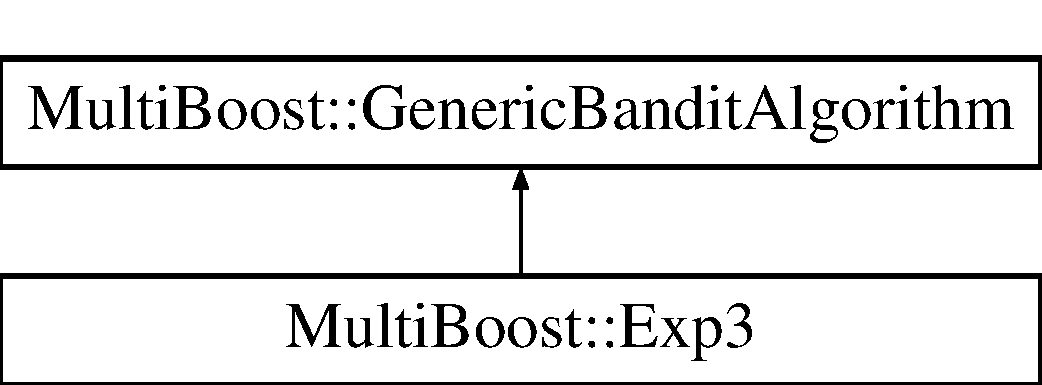
\includegraphics[height=2.000000cm]{classMultiBoost_1_1Exp3}
\end{center}
\end{figure}
\subsection*{Public Member Functions}
\begin{DoxyCompactItemize}
\item 
\hypertarget{classMultiBoost_1_1Exp3_a28581884d9f378f0c8158525a9cee906}{\hyperlink{Defaults_8h_a80184c4fd10ab70a1a17c5f97dcd1563}{Alpha\-Real} {\bfseries get\-Gamma} ()}\label{classMultiBoost_1_1Exp3_a28581884d9f378f0c8158525a9cee906}

\item 
\hypertarget{classMultiBoost_1_1Exp3_af1d818ccfd9369791cca8a796c112791}{void {\bfseries set\-Gamma} (\hyperlink{Defaults_8h_a80184c4fd10ab70a1a17c5f97dcd1563}{Alpha\-Real} gamma)}\label{classMultiBoost_1_1Exp3_af1d818ccfd9369791cca8a796c112791}

\item 
virtual void \hyperlink{classMultiBoost_1_1Exp3_aa478135069d5ac28c57eb096ff5e35b7}{receive\-Reward} (int arm\-Num, \hyperlink{Defaults_8h_a80184c4fd10ab70a1a17c5f97dcd1563}{Alpha\-Real} reward)
\item 
virtual void \hyperlink{classMultiBoost_1_1Exp3_a6c8fa5e1c70b5482e77cc0cd263a37f9}{initialize} (vector$<$ \hyperlink{Defaults_8h_a80184c4fd10ab70a1a17c5f97dcd1563}{Alpha\-Real} $>$ \&vals)
\item 
virtual int \hyperlink{classMultiBoost_1_1Exp3_a7937ade0545a4162e2f7419c38be0a97}{get\-Next\-Action} ()
\item 
virtual void \hyperlink{classMultiBoost_1_1Exp3_adb5f9cc04795a8149153305cacfb525f}{init\-Learning\-Options} (const \hyperlink{classnor__utils_1_1Args}{nor\-\_\-utils\-::\-Args} \&args)
\end{DoxyCompactItemize}
\subsection*{Protected Member Functions}
\begin{DoxyCompactItemize}
\item 
virtual void \hyperlink{classMultiBoost_1_1Exp3_a2dc6188c0ede884c85d4d9c0354f29fa}{updateith\-Value} (int i)
\end{DoxyCompactItemize}
\subsection*{Protected Attributes}
\begin{DoxyCompactItemize}
\item 
\hypertarget{classMultiBoost_1_1Exp3_a069a7f5bcab20426c8f33173c4c0dc11}{\hyperlink{Defaults_8h_a80184c4fd10ab70a1a17c5f97dcd1563}{Alpha\-Real} {\bfseries \-\_\-gamma}}\label{classMultiBoost_1_1Exp3_a069a7f5bcab20426c8f33173c4c0dc11}

\item 
\hypertarget{classMultiBoost_1_1Exp3_aa49aa6b9c02da2bcd2144cc0644a9ac4}{vector$<$ \hyperlink{Defaults_8h_a80184c4fd10ab70a1a17c5f97dcd1563}{Alpha\-Real} $>$ {\bfseries \-\_\-p}}\label{classMultiBoost_1_1Exp3_aa49aa6b9c02da2bcd2144cc0644a9ac4}

\item 
\hypertarget{classMultiBoost_1_1Exp3_a41e68d77caf95c943299c5d49edce528}{vector$<$ \hyperlink{Defaults_8h_a80184c4fd10ab70a1a17c5f97dcd1563}{Alpha\-Real} $>$ {\bfseries \-\_\-p\-Hat}}\label{classMultiBoost_1_1Exp3_a41e68d77caf95c943299c5d49edce528}

\end{DoxyCompactItemize}
\subsection*{Additional Inherited Members}


\subsection{Detailed Description}


Definition at line 129 of file Exp3.\-h.



\subsection{Member Function Documentation}
\hypertarget{classMultiBoost_1_1Exp3_a7937ade0545a4162e2f7419c38be0a97}{\index{Multi\-Boost\-::\-Exp3@{Multi\-Boost\-::\-Exp3}!get\-Next\-Action@{get\-Next\-Action}}
\index{get\-Next\-Action@{get\-Next\-Action}!MultiBoost::Exp3@{Multi\-Boost\-::\-Exp3}}
\subsubsection[{get\-Next\-Action}]{\setlength{\rightskip}{0pt plus 5cm}int Multi\-Boost\-::\-Exp3\-::get\-Next\-Action (
\begin{DoxyParamCaption}
{}
\end{DoxyParamCaption}
)\hspace{0.3cm}{\ttfamily [virtual]}}}\label{classMultiBoost_1_1Exp3_a7937ade0545a4162e2f7419c38be0a97}
Get the best action. \begin{DoxyReturn}{Returns}
The index of arm which then will be pulled. 
\end{DoxyReturn}
\begin{DoxyDate}{Date}
30/03/2010 
\end{DoxyDate}


Implements \hyperlink{classMultiBoost_1_1GenericBanditAlgorithm_a73d90995d4694aa23649dc508527cc8c}{Multi\-Boost\-::\-Generic\-Bandit\-Algorithm}.



Definition at line 66 of file Exp3.\-cpp.

\hypertarget{classMultiBoost_1_1Exp3_a6c8fa5e1c70b5482e77cc0cd263a37f9}{\index{Multi\-Boost\-::\-Exp3@{Multi\-Boost\-::\-Exp3}!initialize@{initialize}}
\index{initialize@{initialize}!MultiBoost::Exp3@{Multi\-Boost\-::\-Exp3}}
\subsubsection[{initialize}]{\setlength{\rightskip}{0pt plus 5cm}void Multi\-Boost\-::\-Exp3\-::initialize (
\begin{DoxyParamCaption}
\item[{vector$<$ {\bf Alpha\-Real} $>$ \&}]{vals}
\end{DoxyParamCaption}
)\hspace{0.3cm}{\ttfamily [virtual]}}}\label{classMultiBoost_1_1Exp3_a6c8fa5e1c70b5482e77cc0cd263a37f9}
A simple interface to initialze the member variables. This function simply sets the flag because all bandit algorithm has an own initialization process. 
\begin{DoxyParams}{Parameters}
{\em vals} & the values for the initalization \\
\hline
\end{DoxyParams}
\begin{DoxyDate}{Date}
30/03/2010 
\end{DoxyDate}


Reimplemented from \hyperlink{classMultiBoost_1_1GenericBanditAlgorithm_a21bb0d3dc368c96135c387783315cc4f}{Multi\-Boost\-::\-Generic\-Bandit\-Algorithm}.



Definition at line 95 of file Exp3.\-cpp.

\hypertarget{classMultiBoost_1_1Exp3_adb5f9cc04795a8149153305cacfb525f}{\index{Multi\-Boost\-::\-Exp3@{Multi\-Boost\-::\-Exp3}!init\-Learning\-Options@{init\-Learning\-Options}}
\index{init\-Learning\-Options@{init\-Learning\-Options}!MultiBoost::Exp3@{Multi\-Boost\-::\-Exp3}}
\subsubsection[{init\-Learning\-Options}]{\setlength{\rightskip}{0pt plus 5cm}void Multi\-Boost\-::\-Exp3\-::init\-Learning\-Options (
\begin{DoxyParamCaption}
\item[{const {\bf nor\-\_\-utils\-::\-Args} \&}]{args}
\end{DoxyParamCaption}
)\hspace{0.3cm}{\ttfamily [virtual]}}}\label{classMultiBoost_1_1Exp3_adb5f9cc04795a8149153305cacfb525f}
Set the arguments of the algorithm using the standard interface of the argument handling (see in the weak learners). Call this to set the arguments given by the user. 
\begin{DoxyParams}{Parameters}
{\em args} & The arguments defined by the user in the command line. \\
\hline
\end{DoxyParams}
\begin{DoxyDate}{Date}
10/03/2010 
\end{DoxyDate}


Implements \hyperlink{classMultiBoost_1_1GenericBanditAlgorithm_a61b051648cee17985a8a8bc0332e8bb9}{Multi\-Boost\-::\-Generic\-Bandit\-Algorithm}.



Definition at line 55 of file Exp3.\-cpp.

\hypertarget{classMultiBoost_1_1Exp3_aa478135069d5ac28c57eb096ff5e35b7}{\index{Multi\-Boost\-::\-Exp3@{Multi\-Boost\-::\-Exp3}!receive\-Reward@{receive\-Reward}}
\index{receive\-Reward@{receive\-Reward}!MultiBoost::Exp3@{Multi\-Boost\-::\-Exp3}}
\subsubsection[{receive\-Reward}]{\setlength{\rightskip}{0pt plus 5cm}void Multi\-Boost\-::\-Exp3\-::receive\-Reward (
\begin{DoxyParamCaption}
\item[{int}]{arm\-Num, }
\item[{{\bf Alpha\-Real}}]{reward}
\end{DoxyParamCaption}
)\hspace{0.3cm}{\ttfamily [virtual]}}}\label{classMultiBoost_1_1Exp3_aa478135069d5ac28c57eb096ff5e35b7}
Receive reward and updates the statistics, i.\-e. the sum of reward of an arm and the number of this arm had been pulled. 
\begin{DoxyParams}{Parameters}
{\em arm\-Num} & The index of arm has been pulled. \\
\hline
{\em reward} & The reward is incurred by the action, i.\-e. pulling an arm. \\
\hline
\end{DoxyParams}
\begin{DoxyDate}{Date}
30/03/2010 
\end{DoxyDate}


Reimplemented from \hyperlink{classMultiBoost_1_1GenericBanditAlgorithm_affd61d12f8dc47d4ad45721562ba60b7}{Multi\-Boost\-::\-Generic\-Bandit\-Algorithm}.



Definition at line 157 of file Exp3.\-cpp.

\hypertarget{classMultiBoost_1_1Exp3_a2dc6188c0ede884c85d4d9c0354f29fa}{\index{Multi\-Boost\-::\-Exp3@{Multi\-Boost\-::\-Exp3}!updateith\-Value@{updateith\-Value}}
\index{updateith\-Value@{updateith\-Value}!MultiBoost::Exp3@{Multi\-Boost\-::\-Exp3}}
\subsubsection[{updateith\-Value}]{\setlength{\rightskip}{0pt plus 5cm}void Multi\-Boost\-::\-Exp3\-::updateith\-Value (
\begin{DoxyParamCaption}
\item[{int}]{arm\-Num}
\end{DoxyParamCaption}
)\hspace{0.3cm}{\ttfamily [protected]}, {\ttfamily [virtual]}}}\label{classMultiBoost_1_1Exp3_a2dc6188c0ede884c85d4d9c0354f29fa}
Update the statics of the arms. In the case of stochastic bandit algorithms it updates the B-\/values, and in the case of adversarials bandit methods it updates the probabilities over the arms. 
\begin{DoxyParams}{Parameters}
{\em arm\-Num} & the index of arm whose statistics will be updated. \\
\hline
\end{DoxyParams}
\begin{DoxyDate}{Date}
10/03/2010 
\end{DoxyDate}


Implements \hyperlink{classMultiBoost_1_1GenericBanditAlgorithm_a46066e41b12d20f0b962d3f46d9b0d22}{Multi\-Boost\-::\-Generic\-Bandit\-Algorithm}.



Definition at line 123 of file Exp3.\-cpp.



The documentation for this class was generated from the following files\-:\begin{DoxyCompactItemize}
\item 
C\-:/\-Users/fradav/\-Documents/\-Dev/\-C++/\-Multiboost/\-Sources/src/\-Bandits/\hyperlink{Exp3_8h}{Exp3.\-h}\item 
C\-:/\-Users/fradav/\-Documents/\-Dev/\-C++/\-Multiboost/\-Sources/src/\-Bandits/Exp3.\-cpp\end{DoxyCompactItemize}

\hypertarget{classMultiBoost_1_1Exp3G}{\section{Multi\-Boost\-:\-:Exp3\-G Class Reference}
\label{classMultiBoost_1_1Exp3G}\index{Multi\-Boost\-::\-Exp3\-G@{Multi\-Boost\-::\-Exp3\-G}}
}
Inheritance diagram for Multi\-Boost\-:\-:Exp3\-G\-:\begin{figure}[H]
\begin{center}
\leavevmode
\includegraphics[height=3.000000cm]{classMultiBoost_1_1Exp3G}
\end{center}
\end{figure}
\subsection*{Public Member Functions}
\begin{DoxyCompactItemize}
\item 
\hypertarget{classMultiBoost_1_1Exp3G_ac3555ffff618368ff300b2fa2d66afd8}{double {\bfseries get\-Eta} ()}\label{classMultiBoost_1_1Exp3G_ac3555ffff618368ff300b2fa2d66afd8}

\item 
\hypertarget{classMultiBoost_1_1Exp3G_a36824f84e85cb68dd482eb95743fe07a}{void {\bfseries set\-Eta} (\hyperlink{Defaults_8h_a80184c4fd10ab70a1a17c5f97dcd1563}{Alpha\-Real} eta)}\label{classMultiBoost_1_1Exp3G_a36824f84e85cb68dd482eb95743fe07a}

\item 
\hypertarget{classMultiBoost_1_1Exp3G_a04245cb775351595d57acd4f430e8b7e}{double {\bfseries get\-Gamma} ()}\label{classMultiBoost_1_1Exp3G_a04245cb775351595d57acd4f430e8b7e}

\item 
\hypertarget{classMultiBoost_1_1Exp3G_a712fa979f4b05c25f64316b83f4fdfb8}{void {\bfseries set\-Gamma} (double gamma)}\label{classMultiBoost_1_1Exp3G_a712fa979f4b05c25f64316b83f4fdfb8}

\item 
virtual void \hyperlink{classMultiBoost_1_1Exp3G_ae741868b98353d0095e6e388dff77372}{receive\-Reward} (int arm\-Num, \hyperlink{Defaults_8h_a80184c4fd10ab70a1a17c5f97dcd1563}{Alpha\-Real} reward)
\item 
virtual void \hyperlink{classMultiBoost_1_1Exp3G_af0a9d437a33cc4bc9c9b24c85dfa0f91}{initialize} (vector$<$ \hyperlink{Defaults_8h_a80184c4fd10ab70a1a17c5f97dcd1563}{Alpha\-Real} $>$ \&vals)
\item 
virtual int \hyperlink{classMultiBoost_1_1Exp3G_a35820a70acd39c4acd3458f72f013bac}{get\-Next\-Action} ()
\item 
virtual void \hyperlink{classMultiBoost_1_1Exp3G_aea72d9f2057818dda38b37727f7de9c2}{init\-Learning\-Options} (const \hyperlink{classnor__utils_1_1Args}{nor\-\_\-utils\-::\-Args} \&args)
\end{DoxyCompactItemize}
\subsection*{Protected Member Functions}
\begin{DoxyCompactItemize}
\item 
virtual void \hyperlink{classMultiBoost_1_1Exp3G_a5ba701c52290894791ff2fcc685df3a3}{updateith\-Value} (int arm)
\end{DoxyCompactItemize}
\subsection*{Protected Attributes}
\begin{DoxyCompactItemize}
\item 
\hypertarget{classMultiBoost_1_1Exp3G_a1016293c08d529acdc668b1cc561cdbe}{\hyperlink{Defaults_8h_a80184c4fd10ab70a1a17c5f97dcd1563}{Alpha\-Real} {\bfseries \-\_\-eta}}\label{classMultiBoost_1_1Exp3G_a1016293c08d529acdc668b1cc561cdbe}

\item 
\hypertarget{classMultiBoost_1_1Exp3G_aea41c6a32ee98a9147c984e6dde58576}{\hyperlink{Defaults_8h_a80184c4fd10ab70a1a17c5f97dcd1563}{Alpha\-Real} {\bfseries \-\_\-gamma}}\label{classMultiBoost_1_1Exp3G_aea41c6a32ee98a9147c984e6dde58576}

\item 
\hypertarget{classMultiBoost_1_1Exp3G_a158e69f5bee912c7ad88a975985724c4}{vector$<$ \hyperlink{Defaults_8h_a80184c4fd10ab70a1a17c5f97dcd1563}{Alpha\-Real} $>$ {\bfseries \-\_\-p}}\label{classMultiBoost_1_1Exp3G_a158e69f5bee912c7ad88a975985724c4}

\item 
\hypertarget{classMultiBoost_1_1Exp3G_a6e0a3f4005860529a1c20f6ee7df6d3f}{vector$<$ \hyperlink{Defaults_8h_a80184c4fd10ab70a1a17c5f97dcd1563}{Alpha\-Real} $>$ {\bfseries \-\_\-w}}\label{classMultiBoost_1_1Exp3G_a6e0a3f4005860529a1c20f6ee7df6d3f}

\item 
\hypertarget{classMultiBoost_1_1Exp3G_a9c05071ae0532479245e9fbde05ca737}{vector$<$ \hyperlink{Defaults_8h_a80184c4fd10ab70a1a17c5f97dcd1563}{Alpha\-Real} $>$ {\bfseries \-\_\-tmp\-W}}\label{classMultiBoost_1_1Exp3G_a9c05071ae0532479245e9fbde05ca737}

\item 
\hypertarget{classMultiBoost_1_1Exp3G_af88e086d17fc20a767430257557c02b8}{vector$<$ vector$<$ int $>$ $>$ {\bfseries \-\_\-side\-Information}}\label{classMultiBoost_1_1Exp3G_af88e086d17fc20a767430257557c02b8}

\item 
\hypertarget{classMultiBoost_1_1Exp3G_af5ff69cc560d458e5ad9c68fa7d86d37}{vector$<$ int $>$ {\bfseries \-\_\-actions}}\label{classMultiBoost_1_1Exp3G_af5ff69cc560d458e5ad9c68fa7d86d37}

\end{DoxyCompactItemize}
\subsection*{Additional Inherited Members}


\subsection{Detailed Description}


Definition at line 59 of file Exp3\-G.\-h.



\subsection{Member Function Documentation}
\hypertarget{classMultiBoost_1_1Exp3G_a35820a70acd39c4acd3458f72f013bac}{\index{Multi\-Boost\-::\-Exp3\-G@{Multi\-Boost\-::\-Exp3\-G}!get\-Next\-Action@{get\-Next\-Action}}
\index{get\-Next\-Action@{get\-Next\-Action}!MultiBoost::Exp3G@{Multi\-Boost\-::\-Exp3\-G}}
\subsubsection[{get\-Next\-Action}]{\setlength{\rightskip}{0pt plus 5cm}int Multi\-Boost\-::\-Exp3\-G\-::get\-Next\-Action (
\begin{DoxyParamCaption}
{}
\end{DoxyParamCaption}
)\hspace{0.3cm}{\ttfamily [virtual]}}}\label{classMultiBoost_1_1Exp3G_a35820a70acd39c4acd3458f72f013bac}
Get the best action. \begin{DoxyReturn}{Returns}
The index of arm which then will be pulled. 
\end{DoxyReturn}
\begin{DoxyDate}{Date}
30/03/2010 
\end{DoxyDate}


Implements \hyperlink{classMultiBoost_1_1GenericBanditAlgorithm_a73d90995d4694aa23649dc508527cc8c}{Multi\-Boost\-::\-Generic\-Bandit\-Algorithm}.



Definition at line 68 of file Exp3\-G.\-cpp.

\hypertarget{classMultiBoost_1_1Exp3G_af0a9d437a33cc4bc9c9b24c85dfa0f91}{\index{Multi\-Boost\-::\-Exp3\-G@{Multi\-Boost\-::\-Exp3\-G}!initialize@{initialize}}
\index{initialize@{initialize}!MultiBoost::Exp3G@{Multi\-Boost\-::\-Exp3\-G}}
\subsubsection[{initialize}]{\setlength{\rightskip}{0pt plus 5cm}void Multi\-Boost\-::\-Exp3\-G\-::initialize (
\begin{DoxyParamCaption}
\item[{vector$<$ {\bf Alpha\-Real} $>$ \&}]{vals}
\end{DoxyParamCaption}
)\hspace{0.3cm}{\ttfamily [virtual]}}}\label{classMultiBoost_1_1Exp3G_af0a9d437a33cc4bc9c9b24c85dfa0f91}
A simple interface to initialze the member variables. This function simply sets the flag because all bandit algorithm has an own initialization process. 
\begin{DoxyParams}{Parameters}
{\em vals} & the values for the initalization \\
\hline
\end{DoxyParams}
\begin{DoxyDate}{Date}
30/03/2010 
\end{DoxyDate}


Reimplemented from \hyperlink{classMultiBoost_1_1GenericBanditAlgorithm_a21bb0d3dc368c96135c387783315cc4f}{Multi\-Boost\-::\-Generic\-Bandit\-Algorithm}.



Reimplemented in \hyperlink{classMultiBoost_1_1Exp3G2_a7851b4a11591d7fcd89cca93d81e9f87}{Multi\-Boost\-::\-Exp3\-G2}, and \hyperlink{classMultiBoost_1_1Exp3P_a108129f4aa9eaf9d6ceab4c87ae76c22}{Multi\-Boost\-::\-Exp3\-P}.



Definition at line 97 of file Exp3\-G.\-cpp.

\hypertarget{classMultiBoost_1_1Exp3G_aea72d9f2057818dda38b37727f7de9c2}{\index{Multi\-Boost\-::\-Exp3\-G@{Multi\-Boost\-::\-Exp3\-G}!init\-Learning\-Options@{init\-Learning\-Options}}
\index{init\-Learning\-Options@{init\-Learning\-Options}!MultiBoost::Exp3G@{Multi\-Boost\-::\-Exp3\-G}}
\subsubsection[{init\-Learning\-Options}]{\setlength{\rightskip}{0pt plus 5cm}void Multi\-Boost\-::\-Exp3\-G\-::init\-Learning\-Options (
\begin{DoxyParamCaption}
\item[{const {\bf nor\-\_\-utils\-::\-Args} \&}]{args}
\end{DoxyParamCaption}
)\hspace{0.3cm}{\ttfamily [virtual]}}}\label{classMultiBoost_1_1Exp3G_aea72d9f2057818dda38b37727f7de9c2}
Set the arguments of the algorithm using the standard interface of the argument handling (see in the weak learners). Call this to set the arguments given by the user. 
\begin{DoxyParams}{Parameters}
{\em args} & The arguments defined by the user in the command line. \\
\hline
\end{DoxyParams}
\begin{DoxyDate}{Date}
10/03/2010 
\end{DoxyDate}


Implements \hyperlink{classMultiBoost_1_1GenericBanditAlgorithm_a61b051648cee17985a8a8bc0332e8bb9}{Multi\-Boost\-::\-Generic\-Bandit\-Algorithm}.



Definition at line 53 of file Exp3\-G.\-cpp.

\hypertarget{classMultiBoost_1_1Exp3G_ae741868b98353d0095e6e388dff77372}{\index{Multi\-Boost\-::\-Exp3\-G@{Multi\-Boost\-::\-Exp3\-G}!receive\-Reward@{receive\-Reward}}
\index{receive\-Reward@{receive\-Reward}!MultiBoost::Exp3G@{Multi\-Boost\-::\-Exp3\-G}}
\subsubsection[{receive\-Reward}]{\setlength{\rightskip}{0pt plus 5cm}void Multi\-Boost\-::\-Exp3\-G\-::receive\-Reward (
\begin{DoxyParamCaption}
\item[{int}]{arm\-Num, }
\item[{{\bf Alpha\-Real}}]{reward}
\end{DoxyParamCaption}
)\hspace{0.3cm}{\ttfamily [virtual]}}}\label{classMultiBoost_1_1Exp3G_ae741868b98353d0095e6e388dff77372}
Receive reward and updates the statistics, i.\-e. the sum of reward of an arm and the number of this arm had been pulled. 
\begin{DoxyParams}{Parameters}
{\em arm\-Num} & The index of arm has been pulled. \\
\hline
{\em reward} & The reward is incurred by the action, i.\-e. pulling an arm. \\
\hline
\end{DoxyParams}
\begin{DoxyDate}{Date}
30/03/2010 
\end{DoxyDate}


Reimplemented from \hyperlink{classMultiBoost_1_1GenericBanditAlgorithm_affd61d12f8dc47d4ad45721562ba60b7}{Multi\-Boost\-::\-Generic\-Bandit\-Algorithm}.



Reimplemented in \hyperlink{classMultiBoost_1_1Exp3G2_a63a055c95b7dddd9bc513d1d78ef0aa4}{Multi\-Boost\-::\-Exp3\-G2}, and \hyperlink{classMultiBoost_1_1Exp3P_a01489e450c6de42354a6ea726599ffff}{Multi\-Boost\-::\-Exp3\-P}.



Definition at line 179 of file Exp3\-G.\-cpp.

\hypertarget{classMultiBoost_1_1Exp3G_a5ba701c52290894791ff2fcc685df3a3}{\index{Multi\-Boost\-::\-Exp3\-G@{Multi\-Boost\-::\-Exp3\-G}!updateith\-Value@{updateith\-Value}}
\index{updateith\-Value@{updateith\-Value}!MultiBoost::Exp3G@{Multi\-Boost\-::\-Exp3\-G}}
\subsubsection[{updateith\-Value}]{\setlength{\rightskip}{0pt plus 5cm}void Multi\-Boost\-::\-Exp3\-G\-::updateith\-Value (
\begin{DoxyParamCaption}
\item[{int}]{arm\-Num}
\end{DoxyParamCaption}
)\hspace{0.3cm}{\ttfamily [protected]}, {\ttfamily [virtual]}}}\label{classMultiBoost_1_1Exp3G_a5ba701c52290894791ff2fcc685df3a3}
Update the statics of the arms. In the case of stochastic bandit algorithms it updates the B-\/values, and in the case of adversarials bandit methods it updates the probabilities over the arms. 
\begin{DoxyParams}{Parameters}
{\em arm\-Num} & the index of arm whose statistics will be updated. \\
\hline
\end{DoxyParams}
\begin{DoxyDate}{Date}
10/03/2010 
\end{DoxyDate}


Implements \hyperlink{classMultiBoost_1_1GenericBanditAlgorithm_a46066e41b12d20f0b962d3f46d9b0d22}{Multi\-Boost\-::\-Generic\-Bandit\-Algorithm}.



Definition at line 150 of file Exp3\-G.\-cpp.



The documentation for this class was generated from the following files\-:\begin{DoxyCompactItemize}
\item 
C\-:/\-Users/fradav/\-Documents/\-Dev/\-C++/\-Multiboost/\-Sources/src/\-Bandits/Exp3\-G.\-h\item 
C\-:/\-Users/fradav/\-Documents/\-Dev/\-C++/\-Multiboost/\-Sources/src/\-Bandits/Exp3\-G.\-cpp\end{DoxyCompactItemize}

\hypertarget{classMultiBoost_1_1Exp3G2}{\section{Multi\-Boost\-:\-:Exp3\-G2 Class Reference}
\label{classMultiBoost_1_1Exp3G2}\index{Multi\-Boost\-::\-Exp3\-G2@{Multi\-Boost\-::\-Exp3\-G2}}
}
Inheritance diagram for Multi\-Boost\-:\-:Exp3\-G2\-:\begin{figure}[H]
\begin{center}
\leavevmode
\includegraphics[height=3.000000cm]{classMultiBoost_1_1Exp3G2}
\end{center}
\end{figure}
\subsection*{Public Member Functions}
\begin{DoxyCompactItemize}
\item 
virtual void \hyperlink{classMultiBoost_1_1Exp3G2_a63a055c95b7dddd9bc513d1d78ef0aa4}{receive\-Reward} (int arm\-Num, \hyperlink{Defaults_8h_a80184c4fd10ab70a1a17c5f97dcd1563}{Alpha\-Real} reward)
\item 
\hypertarget{classMultiBoost_1_1Exp3G2_a497f296e281816d20cb3b0c4e32468af}{virtual void {\bfseries receive\-Reward} (vector$<$ \hyperlink{Defaults_8h_a80184c4fd10ab70a1a17c5f97dcd1563}{Alpha\-Real} $>$ reward)}\label{classMultiBoost_1_1Exp3G2_a497f296e281816d20cb3b0c4e32468af}

\item 
virtual void \hyperlink{classMultiBoost_1_1Exp3G2_a7851b4a11591d7fcd89cca93d81e9f87}{initialize} (vector$<$ \hyperlink{Defaults_8h_a80184c4fd10ab70a1a17c5f97dcd1563}{Alpha\-Real} $>$ \&vals)
\end{DoxyCompactItemize}
\subsection*{Additional Inherited Members}


\subsection{Detailed Description}


Definition at line 60 of file Exp3\-G2.\-h.



\subsection{Member Function Documentation}
\hypertarget{classMultiBoost_1_1Exp3G2_a7851b4a11591d7fcd89cca93d81e9f87}{\index{Multi\-Boost\-::\-Exp3\-G2@{Multi\-Boost\-::\-Exp3\-G2}!initialize@{initialize}}
\index{initialize@{initialize}!MultiBoost::Exp3G2@{Multi\-Boost\-::\-Exp3\-G2}}
\subsubsection[{initialize}]{\setlength{\rightskip}{0pt plus 5cm}void Multi\-Boost\-::\-Exp3\-G2\-::initialize (
\begin{DoxyParamCaption}
\item[{vector$<$ {\bf Alpha\-Real} $>$ \&}]{vals}
\end{DoxyParamCaption}
)\hspace{0.3cm}{\ttfamily [virtual]}}}\label{classMultiBoost_1_1Exp3G2_a7851b4a11591d7fcd89cca93d81e9f87}
A simple interface to initialze the member variables. This function simply sets the flag because all bandit algorithm has an own initialization process. 
\begin{DoxyParams}{Parameters}
{\em vals} & the values for the initalization \\
\hline
\end{DoxyParams}
\begin{DoxyDate}{Date}
30/03/2010 
\end{DoxyDate}


Reimplemented from \hyperlink{classMultiBoost_1_1Exp3G_af0a9d437a33cc4bc9c9b24c85dfa0f91}{Multi\-Boost\-::\-Exp3\-G}.



Definition at line 54 of file Exp3\-G2.\-cpp.

\hypertarget{classMultiBoost_1_1Exp3G2_a63a055c95b7dddd9bc513d1d78ef0aa4}{\index{Multi\-Boost\-::\-Exp3\-G2@{Multi\-Boost\-::\-Exp3\-G2}!receive\-Reward@{receive\-Reward}}
\index{receive\-Reward@{receive\-Reward}!MultiBoost::Exp3G2@{Multi\-Boost\-::\-Exp3\-G2}}
\subsubsection[{receive\-Reward}]{\setlength{\rightskip}{0pt plus 5cm}void Multi\-Boost\-::\-Exp3\-G2\-::receive\-Reward (
\begin{DoxyParamCaption}
\item[{int}]{arm\-Num, }
\item[{{\bf Alpha\-Real}}]{reward}
\end{DoxyParamCaption}
)\hspace{0.3cm}{\ttfamily [virtual]}}}\label{classMultiBoost_1_1Exp3G2_a63a055c95b7dddd9bc513d1d78ef0aa4}
Receive reward and updates the statistics, i.\-e. the sum of reward of an arm and the number of this arm had been pulled. 
\begin{DoxyParams}{Parameters}
{\em arm\-Num} & The index of arm has been pulled. \\
\hline
{\em reward} & The reward is incurred by the action, i.\-e. pulling an arm. \\
\hline
\end{DoxyParams}
\begin{DoxyDate}{Date}
30/03/2010 
\end{DoxyDate}


Reimplemented from \hyperlink{classMultiBoost_1_1Exp3G_ae741868b98353d0095e6e388dff77372}{Multi\-Boost\-::\-Exp3\-G}.



Definition at line 81 of file Exp3\-G2.\-cpp.



The documentation for this class was generated from the following files\-:\begin{DoxyCompactItemize}
\item 
C\-:/\-Users/fradav/\-Documents/\-Dev/\-C++/\-Multiboost/\-Sources/src/\-Bandits/Exp3\-G2.\-h\item 
C\-:/\-Users/fradav/\-Documents/\-Dev/\-C++/\-Multiboost/\-Sources/src/\-Bandits/Exp3\-G2.\-cpp\end{DoxyCompactItemize}

\hypertarget{classMultiBoost_1_1Exp3GLS}{\section{Multi\-Boost\-:\-:Exp3\-G\-L\-S$<$ Base\-Type, Key\-Type $>$ Class Template Reference}
\label{classMultiBoost_1_1Exp3GLS}\index{Multi\-Boost\-::\-Exp3\-G\-L\-S$<$ Base\-Type, Key\-Type $>$@{Multi\-Boost\-::\-Exp3\-G\-L\-S$<$ Base\-Type, Key\-Type $>$}}
}
Inheritance diagram for Multi\-Boost\-:\-:Exp3\-G\-L\-S$<$ Base\-Type, Key\-Type $>$\-:\begin{figure}[H]
\begin{center}
\leavevmode
\includegraphics[height=3.000000cm]{classMultiBoost_1_1Exp3GLS}
\end{center}
\end{figure}
\subsection*{Public Member Functions}
\begin{DoxyCompactItemize}
\item 
\hypertarget{classMultiBoost_1_1Exp3GLS_adc9cfcad4a49de23d77f5412cb2a2473}{Key\-Type {\bfseries get\-Previous\-Action} ()}\label{classMultiBoost_1_1Exp3GLS_adc9cfcad4a49de23d77f5412cb2a2473}

\item 
\hypertarget{classMultiBoost_1_1Exp3GLS_a03611a9051397e6134f01d78cf52c695}{void {\bfseries set\-Previous\-Action} (Key\-Type key)}\label{classMultiBoost_1_1Exp3GLS_a03611a9051397e6134f01d78cf52c695}

\item 
\hypertarget{classMultiBoost_1_1Exp3GLS_aa8229ee1d39c2de05c9b32f94d775b48}{virtual void {\bfseries receive\-Reward} (Key\-Type key, Base\-Type reward)}\label{classMultiBoost_1_1Exp3GLS_aa8229ee1d39c2de05c9b32f94d775b48}

\item 
\hypertarget{classMultiBoost_1_1Exp3GLS_ac09401422c11556470cb22a7109aa374}{virtual void {\bfseries initialize} (map$<$ Key\-Type, Base\-Type $>$ \&vals)}\label{classMultiBoost_1_1Exp3GLS_ac09401422c11556470cb22a7109aa374}

\end{DoxyCompactItemize}
\subsection*{Protected Types}
\begin{DoxyCompactItemize}
\item 
\hypertarget{classMultiBoost_1_1Exp3GLS_a3abfa9d81028af38ccc77c94e7ead119}{typedef pair$<$ Base\-Type, Key\-Type $>$ {\bfseries p\-Base\-Key}}\label{classMultiBoost_1_1Exp3GLS_a3abfa9d81028af38ccc77c94e7ead119}

\item 
\hypertarget{classMultiBoost_1_1Exp3GLS_ac8438536c093e9198e6ddd99966dee11}{typedef vector$<$ p\-Base\-Key $>$ {\bfseries vec\-Base\-Key}}\label{classMultiBoost_1_1Exp3GLS_ac8438536c093e9198e6ddd99966dee11}

\item 
\hypertarget{classMultiBoost_1_1Exp3GLS_a90682a64c88412b1b4ab1bfc19ea8961}{typedef vector$<$ p\-Base\-Key $>$\\*
\-::iterator {\bfseries it\-Vector\-Pair\-Base\-Key}}\label{classMultiBoost_1_1Exp3GLS_a90682a64c88412b1b4ab1bfc19ea8961}

\item 
\hypertarget{classMultiBoost_1_1Exp3GLS_a59a624841ce47f5caa85549fabb3818e}{typedef map$<$ Key\-Type, Base\-Type $>$ {\bfseries map\-Key\-Base}}\label{classMultiBoost_1_1Exp3GLS_a59a624841ce47f5caa85549fabb3818e}

\item 
\hypertarget{classMultiBoost_1_1Exp3GLS_a8857d4c8f5b146d211859b8e918dfe63}{typedef map$<$ Key\-Type, Base\-Type $>$\\*
\-::iterator {\bfseries it\-Map\-Key\-Base}}\label{classMultiBoost_1_1Exp3GLS_a8857d4c8f5b146d211859b8e918dfe63}

\item 
\hypertarget{classMultiBoost_1_1Exp3GLS_ab490c29d87d3c87b3faeef5192a9dfbb}{typedef set$<$ Key\-Type $>$\-::iterator {\bfseries it\-Set\-Key}}\label{classMultiBoost_1_1Exp3GLS_ab490c29d87d3c87b3faeef5192a9dfbb}

\item 
\hypertarget{classMultiBoost_1_1Exp3GLS_a3ce77164624293b4eab5b8bc13db395f}{typedef set$<$ Key\-Type $>$ {\bfseries set\-Key}}\label{classMultiBoost_1_1Exp3GLS_a3ce77164624293b4eab5b8bc13db395f}

\item 
\hypertarget{classMultiBoost_1_1Exp3GLS_a481df1b39db9b7aebf0cf6f3df497b2a}{typedef map$<$ Key\-Type, set\-Key $>$ {\bfseries map\-Key\-Set\-Key}}\label{classMultiBoost_1_1Exp3GLS_a481df1b39db9b7aebf0cf6f3df497b2a}

\item 
\hypertarget{classMultiBoost_1_1Exp3GLS_a4b58cc485c723fdde823e5a81e932962}{typedef pair$<$ Key\-Type, Key\-Type $>$ {\bfseries p\-Keys}}\label{classMultiBoost_1_1Exp3GLS_a4b58cc485c723fdde823e5a81e932962}

\item 
\hypertarget{classMultiBoost_1_1Exp3GLS_a3b04960b489fa6429038fea8c57d50a8}{typedef map$<$ p\-Keys, Base\-Type $>$ {\bfseries map\-Key\-Pairs\-Base}}\label{classMultiBoost_1_1Exp3GLS_a3b04960b489fa6429038fea8c57d50a8}

\end{DoxyCompactItemize}
\subsection*{Protected Attributes}
\begin{DoxyCompactItemize}
\item 
\hypertarget{classMultiBoost_1_1Exp3GLS_a9d12aedf8a8b1ab337f8a6b4b62efcf9}{map\-Key\-Pairs\-Base {\bfseries \-\_\-side\-Information}}\label{classMultiBoost_1_1Exp3GLS_a9d12aedf8a8b1ab337f8a6b4b62efcf9}

\item 
\hypertarget{classMultiBoost_1_1Exp3GLS_a00ccd3d395374af918cf2677d8280804}{map\-Key\-Set\-Key {\bfseries \-\_\-consecutive\-Key\-Stat}}\label{classMultiBoost_1_1Exp3GLS_a00ccd3d395374af918cf2677d8280804}

\item 
\hypertarget{classMultiBoost_1_1Exp3GLS_ab75d596d8de4ac353f216e94fabd1ae4}{Key\-Type {\bfseries \-\_\-previous\-Action}}\label{classMultiBoost_1_1Exp3GLS_ab75d596d8de4ac353f216e94fabd1ae4}

\item 
\hypertarget{classMultiBoost_1_1Exp3GLS_ae25e36921abf3dafe024fa49577c98b7}{Base\-Type {\bfseries \-\_\-eta}}\label{classMultiBoost_1_1Exp3GLS_ae25e36921abf3dafe024fa49577c98b7}

\end{DoxyCompactItemize}
\subsection*{Additional Inherited Members}


\subsection{Detailed Description}
\subsubsection*{template$<$typename Base\-Type = double, typename Key\-Type = int$>$class Multi\-Boost\-::\-Exp3\-G\-L\-S$<$ Base\-Type, Key\-Type $>$}



Definition at line 72 of file Exp3\-G\-L\-S.\-h.



The documentation for this class was generated from the following file\-:\begin{DoxyCompactItemize}
\item 
C\-:/\-Users/fradav/\-Documents/\-Dev/\-C++/\-Multiboost/\-Sources/src/\-Bandits\-L\-S/Exp3\-G\-L\-S.\-h\end{DoxyCompactItemize}

\hypertarget{classMultiBoost_1_1Exp3LS}{\section{Multi\-Boost\-:\-:Exp3\-L\-S$<$ Base\-Type, Key\-Type $>$ Class Template Reference}
\label{classMultiBoost_1_1Exp3LS}\index{Multi\-Boost\-::\-Exp3\-L\-S$<$ Base\-Type, Key\-Type $>$@{Multi\-Boost\-::\-Exp3\-L\-S$<$ Base\-Type, Key\-Type $>$}}
}
Inheritance diagram for Multi\-Boost\-:\-:Exp3\-L\-S$<$ Base\-Type, Key\-Type $>$\-:\begin{figure}[H]
\begin{center}
\leavevmode
\includegraphics[height=3.000000cm]{classMultiBoost_1_1Exp3LS}
\end{center}
\end{figure}
\subsection*{Public Member Functions}
\begin{DoxyCompactItemize}
\item 
\hypertarget{classMultiBoost_1_1Exp3LS_a167a1e49537b04d314bbe62a71cca1f3}{Base\-Type {\bfseries get\-Gamma} ()}\label{classMultiBoost_1_1Exp3LS_a167a1e49537b04d314bbe62a71cca1f3}

\item 
\hypertarget{classMultiBoost_1_1Exp3LS_a2d6bdb1e914f41fd02fd66a47e2eeed0}{void {\bfseries set\-Gamma} (Base\-Type gamma)}\label{classMultiBoost_1_1Exp3LS_a2d6bdb1e914f41fd02fd66a47e2eeed0}

\item 
\hypertarget{classMultiBoost_1_1Exp3LS_af9b4f88144a99fd7d66905861d7d3d43}{virtual void {\bfseries receive\-Reward} (Key\-Type key, Base\-Type reward)}\label{classMultiBoost_1_1Exp3LS_af9b4f88144a99fd7d66905861d7d3d43}

\item 
\hypertarget{classMultiBoost_1_1Exp3LS_a7d9f285d5479e21f9ea1adab87a43f7d}{virtual void {\bfseries initialize} (map$<$ Key\-Type, Base\-Type $>$ \&vals)}\label{classMultiBoost_1_1Exp3LS_a7d9f285d5479e21f9ea1adab87a43f7d}

\item 
\hypertarget{classMultiBoost_1_1Exp3LS_a2cf13b6ca2e2ff3c419b4fead2cfa5df}{virtual Key\-Type {\bfseries get\-Next\-Action} (Key\-Type default\-Value)}\label{classMultiBoost_1_1Exp3LS_a2cf13b6ca2e2ff3c419b4fead2cfa5df}

\end{DoxyCompactItemize}
\subsection*{Protected Types}
\begin{DoxyCompactItemize}
\item 
\hypertarget{classMultiBoost_1_1Exp3LS_a56cf772f45842cf82f412617a89c4157}{typedef pair$<$ Base\-Type, Key\-Type $>$ {\bfseries p\-Base\-Key}}\label{classMultiBoost_1_1Exp3LS_a56cf772f45842cf82f412617a89c4157}

\item 
\hypertarget{classMultiBoost_1_1Exp3LS_ab47ecaca2c75ed93535da0208eed0a00}{typedef vector$<$ p\-Base\-Key $>$ {\bfseries vec\-Base\-Key}}\label{classMultiBoost_1_1Exp3LS_ab47ecaca2c75ed93535da0208eed0a00}

\item 
\hypertarget{classMultiBoost_1_1Exp3LS_a02d60b4864ffdb98f81cab146a34afcf}{typedef vector$<$ p\-Base\-Key $>$\\*
\-::iterator {\bfseries it\-Vector\-Pair\-Base\-Key}}\label{classMultiBoost_1_1Exp3LS_a02d60b4864ffdb98f81cab146a34afcf}

\item 
\hypertarget{classMultiBoost_1_1Exp3LS_a61c4f9184a570de2d1dbfd13ec8457d8}{typedef map$<$ Key\-Type, Base\-Type $>$ {\bfseries map\-Key\-Base}}\label{classMultiBoost_1_1Exp3LS_a61c4f9184a570de2d1dbfd13ec8457d8}

\item 
\hypertarget{classMultiBoost_1_1Exp3LS_a5d1ee59548ecd78a99ae4fe6d4782207}{typedef map$<$ Key\-Type, Base\-Type $>$\\*
\-::iterator {\bfseries it\-Map\-Key\-Base}}\label{classMultiBoost_1_1Exp3LS_a5d1ee59548ecd78a99ae4fe6d4782207}

\item 
\hypertarget{classMultiBoost_1_1Exp3LS_aa7379cc046bfee84de02b46f844d7d76}{typedef set$<$ Key\-Type $>$\-::iterator {\bfseries it\-Set\-Key}}\label{classMultiBoost_1_1Exp3LS_aa7379cc046bfee84de02b46f844d7d76}

\end{DoxyCompactItemize}
\subsection*{Protected Member Functions}
\begin{DoxyCompactItemize}
\item 
\hypertarget{classMultiBoost_1_1Exp3LS_a2ba8dda6c4af4ce06b8997c693fd4209}{virtual void {\bfseries updateith\-Value} (Key\-Type key)}\label{classMultiBoost_1_1Exp3LS_a2ba8dda6c4af4ce06b8997c693fd4209}

\item 
\hypertarget{classMultiBoost_1_1Exp3LS_a9510a6f2cb484c543afa3db475737543}{virtual Base\-Type {\bfseries get\-P\-Value} (Key\-Type key)}\label{classMultiBoost_1_1Exp3LS_a9510a6f2cb484c543afa3db475737543}

\end{DoxyCompactItemize}
\subsection*{Protected Attributes}
\begin{DoxyCompactItemize}
\item 
\hypertarget{classMultiBoost_1_1Exp3LS_a5fc60747afc993252cf549a327dfaa16}{Base\-Type {\bfseries \-\_\-gamma}}\label{classMultiBoost_1_1Exp3LS_a5fc60747afc993252cf549a327dfaa16}

\item 
\hypertarget{classMultiBoost_1_1Exp3LS_a0e3fe9ed00e26bd5359705acc2b4a364}{map$<$ Key\-Type, Base\-Type $>$ {\bfseries \-\_\-p}}\label{classMultiBoost_1_1Exp3LS_a0e3fe9ed00e26bd5359705acc2b4a364}

\item 
\hypertarget{classMultiBoost_1_1Exp3LS_a14cb5849a0bb1413a1d7736105f0fad3}{double {\bfseries \-\_\-\-Xsum}}\label{classMultiBoost_1_1Exp3LS_a14cb5849a0bb1413a1d7736105f0fad3}

\item 
\hypertarget{classMultiBoost_1_1Exp3LS_ad20fa8992e3284643994a1690e62758f}{double {\bfseries \-\_\-expsum}}\label{classMultiBoost_1_1Exp3LS_ad20fa8992e3284643994a1690e62758f}

\item 
\hypertarget{classMultiBoost_1_1Exp3LS_aa8e2fcaf726ba074138e446c2d59d180}{vec\-Base\-Key {\bfseries \-\_\-cum\-Sum}}\label{classMultiBoost_1_1Exp3LS_aa8e2fcaf726ba074138e446c2d59d180}

\end{DoxyCompactItemize}


\subsection{Detailed Description}
\subsubsection*{template$<$typename Base\-Type = double, typename Key\-Type = int$>$class Multi\-Boost\-::\-Exp3\-L\-S$<$ Base\-Type, Key\-Type $>$}



Definition at line 76 of file Exp3\-L\-S.\-h.



The documentation for this class was generated from the following file\-:\begin{DoxyCompactItemize}
\item 
C\-:/\-Users/fradav/\-Documents/\-Dev/\-C++/\-Multiboost/\-Sources/src/\-Bandits\-L\-S/Exp3\-L\-S.\-h\end{DoxyCompactItemize}

\hypertarget{classMultiBoost_1_1Exp3P}{\section{Multi\-Boost\-:\-:Exp3\-P Class Reference}
\label{classMultiBoost_1_1Exp3P}\index{Multi\-Boost\-::\-Exp3\-P@{Multi\-Boost\-::\-Exp3\-P}}
}
Inheritance diagram for Multi\-Boost\-:\-:Exp3\-P\-:\begin{figure}[H]
\begin{center}
\leavevmode
\includegraphics[height=3.000000cm]{classMultiBoost_1_1Exp3P}
\end{center}
\end{figure}
\subsection*{Public Member Functions}
\begin{DoxyCompactItemize}
\item 
virtual void \hyperlink{classMultiBoost_1_1Exp3P_a01489e450c6de42354a6ea726599ffff}{receive\-Reward} (int arm\-Num, \hyperlink{Defaults_8h_a80184c4fd10ab70a1a17c5f97dcd1563}{Alpha\-Real} reward)
\item 
virtual void \hyperlink{classMultiBoost_1_1Exp3P_a108129f4aa9eaf9d6ceab4c87ae76c22}{initialize} (vector$<$ \hyperlink{Defaults_8h_a80184c4fd10ab70a1a17c5f97dcd1563}{Alpha\-Real} $>$ \&vals)
\end{DoxyCompactItemize}
\subsection*{Protected Attributes}
\begin{DoxyCompactItemize}
\item 
\hypertarget{classMultiBoost_1_1Exp3P_ad66c466b559922f5b3cd25974627aea3}{double {\bfseries \-\_\-horizon}}\label{classMultiBoost_1_1Exp3P_ad66c466b559922f5b3cd25974627aea3}

\end{DoxyCompactItemize}
\subsection*{Additional Inherited Members}


\subsection{Detailed Description}


Definition at line 55 of file Exp3\-P.\-h.



\subsection{Member Function Documentation}
\hypertarget{classMultiBoost_1_1Exp3P_a108129f4aa9eaf9d6ceab4c87ae76c22}{\index{Multi\-Boost\-::\-Exp3\-P@{Multi\-Boost\-::\-Exp3\-P}!initialize@{initialize}}
\index{initialize@{initialize}!MultiBoost::Exp3P@{Multi\-Boost\-::\-Exp3\-P}}
\subsubsection[{initialize}]{\setlength{\rightskip}{0pt plus 5cm}void Multi\-Boost\-::\-Exp3\-P\-::initialize (
\begin{DoxyParamCaption}
\item[{vector$<$ {\bf Alpha\-Real} $>$ \&}]{vals}
\end{DoxyParamCaption}
)\hspace{0.3cm}{\ttfamily [virtual]}}}\label{classMultiBoost_1_1Exp3P_a108129f4aa9eaf9d6ceab4c87ae76c22}
A simple interface to initialze the member variables. This function simply sets the flag because all bandit algorithm has an own initialization process. 
\begin{DoxyParams}{Parameters}
{\em vals} & the values for the initalization \\
\hline
\end{DoxyParams}
\begin{DoxyDate}{Date}
30/03/2010 
\end{DoxyDate}


Reimplemented from \hyperlink{classMultiBoost_1_1Exp3G_af0a9d437a33cc4bc9c9b24c85dfa0f91}{Multi\-Boost\-::\-Exp3\-G}.



Definition at line 57 of file Exp3\-P.\-cpp.

\hypertarget{classMultiBoost_1_1Exp3P_a01489e450c6de42354a6ea726599ffff}{\index{Multi\-Boost\-::\-Exp3\-P@{Multi\-Boost\-::\-Exp3\-P}!receive\-Reward@{receive\-Reward}}
\index{receive\-Reward@{receive\-Reward}!MultiBoost::Exp3P@{Multi\-Boost\-::\-Exp3\-P}}
\subsubsection[{receive\-Reward}]{\setlength{\rightskip}{0pt plus 5cm}void Multi\-Boost\-::\-Exp3\-P\-::receive\-Reward (
\begin{DoxyParamCaption}
\item[{int}]{arm\-Num, }
\item[{{\bf Alpha\-Real}}]{reward}
\end{DoxyParamCaption}
)\hspace{0.3cm}{\ttfamily [virtual]}}}\label{classMultiBoost_1_1Exp3P_a01489e450c6de42354a6ea726599ffff}
Receive reward and updates the statistics, i.\-e. the sum of reward of an arm and the number of this arm had been pulled. 
\begin{DoxyParams}{Parameters}
{\em arm\-Num} & The index of arm has been pulled. \\
\hline
{\em reward} & The reward is incurred by the action, i.\-e. pulling an arm. \\
\hline
\end{DoxyParams}
\begin{DoxyDate}{Date}
30/03/2010 
\end{DoxyDate}


Reimplemented from \hyperlink{classMultiBoost_1_1Exp3G_ae741868b98353d0095e6e388dff77372}{Multi\-Boost\-::\-Exp3\-G}.



Definition at line 87 of file Exp3\-P.\-cpp.



The documentation for this class was generated from the following files\-:\begin{DoxyCompactItemize}
\item 
C\-:/\-Users/fradav/\-Documents/\-Dev/\-C++/\-Multiboost/\-Sources/src/\-Bandits/Exp3\-P.\-h\item 
C\-:/\-Users/fradav/\-Documents/\-Dev/\-C++/\-Multiboost/\-Sources/src/\-Bandits/Exp3\-P.\-cpp\end{DoxyCompactItemize}

\hypertarget{structMultiBoost_1_1FeatureDataUCBV}{
\section{MultiBoost::FeatureDataUCBV Struct Reference}
\label{structMultiBoost_1_1FeatureDataUCBV}\index{MultiBoost::FeatureDataUCBV@{MultiBoost::FeatureDataUCBV}}
}
\subsection*{Public Attributes}
\begin{DoxyCompactItemize}
\item 
\hypertarget{structMultiBoost_1_1FeatureDataUCBV_aeecad3af86e208d283c0b621fa84b183}{
int {\bfseries T}}
\label{structMultiBoost_1_1FeatureDataUCBV_aeecad3af86e208d283c0b621fa84b183}

\item 
\hypertarget{structMultiBoost_1_1FeatureDataUCBV_aec0878eddb9fb60b0e7750ef68828646}{
vector$<$ \hyperlink{Defaults_8h_a3a11cfe6a5d469d921716ca6291e934f}{FeatureReal} $>$ {\bfseries X}}
\label{structMultiBoost_1_1FeatureDataUCBV_aec0878eddb9fb60b0e7750ef68828646}

\end{DoxyCompactItemize}


\subsection{Detailed Description}


Definition at line 56 of file UCBVHaarSingleStumpLearner.h.



The documentation for this struct was generated from the following file:\begin{DoxyCompactItemize}
\item 
/cygdrive/c/Users/fradav/Documents/Dev/Multiboost/Sources/src/WeakLearners/\hyperlink{UCBVHaarSingleStumpLearner_8h}{UCBVHaarSingleStumpLearner.h}\end{DoxyCompactItemize}

\hypertarget{classMultiBoost_1_1HaarFeature_1_1FeaturesRegs}{
\section{MultiBoost::HaarFeature::FeaturesRegs Class Reference}
\label{classMultiBoost_1_1HaarFeature_1_1FeaturesRegs}\index{MultiBoost::HaarFeature::FeaturesRegs@{MultiBoost::HaarFeature::FeaturesRegs}}
}


{\ttfamily \#include $<$HaarFeatures.h$>$}

\subsection*{Public Member Functions}
\begin{DoxyCompactItemize}
\item 
void \hyperlink{classMultiBoost_1_1HaarFeature_1_1FeaturesRegs_a23dec729a5b9e7e4fdbc1ea3eeb3d5e8}{addFeature} (const string \&shortName, \hyperlink{classMultiBoost_1_1HaarFeature}{HaarFeature} $\ast$pFeatureToRegister)
\item 
bool \hyperlink{classMultiBoost_1_1HaarFeature_1_1FeaturesRegs_a0d6b0b4a000a5763c32f137aef483593}{hasFeature} (const string \&shortName)
\item 
\hyperlink{classMultiBoost_1_1HaarFeature}{HaarFeature} $\ast$ \hyperlink{classMultiBoost_1_1HaarFeature_1_1FeaturesRegs_aabf4b0ffdcaa11b508bff0d4d59cc839}{getFeature} (const string \&shortName)
\item 
string \hyperlink{classMultiBoost_1_1HaarFeature_1_1FeaturesRegs_a68f555cd74a8f2abc8c85943a2b2c87b}{getRegString} ()
\end{DoxyCompactItemize}


\subsection{Detailed Description}
Holds the information about the registered Haar features. Works pretty much like a class factory. \begin{DoxySeeAlso}{See also}
\hyperlink{HaarFeatures_8h_adcc549bcab1fba9c2649737e60dd50ea}{REGISTER\_\-HAAR\_\-FEATURE} 
\end{DoxySeeAlso}


Definition at line 128 of file HaarFeatures.h.



\subsection{Member Function Documentation}
\hypertarget{classMultiBoost_1_1HaarFeature_1_1FeaturesRegs_a23dec729a5b9e7e4fdbc1ea3eeb3d5e8}{
\index{MultiBoost::HaarFeature::FeaturesRegs@{MultiBoost::HaarFeature::FeaturesRegs}!addFeature@{addFeature}}
\index{addFeature@{addFeature}!MultiBoost::HaarFeature::FeaturesRegs@{MultiBoost::HaarFeature::FeaturesRegs}}
\subsubsection[{addFeature}]{\setlength{\rightskip}{0pt plus 5cm}void MultiBoost::HaarFeature::FeaturesRegs::addFeature (
\begin{DoxyParamCaption}
\item[{const string \&}]{shortName, }
\item[{{\bf HaarFeature} $\ast$}]{pFeatureToRegister}
\end{DoxyParamCaption}
)\hspace{0.3cm}{\ttfamily  \mbox{[}inline\mbox{]}}}}
\label{classMultiBoost_1_1HaarFeature_1_1FeaturesRegs_a23dec729a5b9e7e4fdbc1ea3eeb3d5e8}
Add a feature type to the list of the registered features. 
\begin{DoxyParams}{Parameters}
{\em shortName} & The short name of the feature type. It will be used to retrieve it when necessary. \\
\hline
{\em pFeatureToRegister} & The pointer to the object that contain the feature to be registered. The object will be an instantiation of the derived type from which, thanks to the method {\itshape \hyperlink{classMultiBoost_1_1HaarFeature_a298d8950cb415b3b54b1ad99f54ea6bb}{HaarFeature::create()}\/} it will be possible to obtain other objects of the same derived type. \\
\hline
\end{DoxyParams}
\begin{DoxyDate}{Date}
27/12/2005 
\end{DoxyDate}


Definition at line 142 of file HaarFeatures.h.

\hypertarget{classMultiBoost_1_1HaarFeature_1_1FeaturesRegs_aabf4b0ffdcaa11b508bff0d4d59cc839}{
\index{MultiBoost::HaarFeature::FeaturesRegs@{MultiBoost::HaarFeature::FeaturesRegs}!getFeature@{getFeature}}
\index{getFeature@{getFeature}!MultiBoost::HaarFeature::FeaturesRegs@{MultiBoost::HaarFeature::FeaturesRegs}}
\subsubsection[{getFeature}]{\setlength{\rightskip}{0pt plus 5cm}{\bf HaarFeature}$\ast$ MultiBoost::HaarFeature::FeaturesRegs::getFeature (
\begin{DoxyParamCaption}
\item[{const string \&}]{shortName}
\end{DoxyParamCaption}
)\hspace{0.3cm}{\ttfamily  \mbox{[}inline\mbox{]}}}}
\label{classMultiBoost_1_1HaarFeature_1_1FeaturesRegs_aabf4b0ffdcaa11b508bff0d4d59cc839}
Get the registered object with the given shortName. 
\begin{DoxyParams}{Parameters}
{\em shortName} & The short name of the feature type. \\
\hline
\end{DoxyParams}
\begin{DoxyReturn}{Returns}
The object of the registered feature. 
\end{DoxyReturn}
\begin{DoxySeeAlso}{See also}
\hyperlink{classMultiBoost_1_1HaarFeature_1_1FeaturesRegs_a23dec729a5b9e7e4fdbc1ea3eeb3d5e8}{addFeature} 
\end{DoxySeeAlso}
\begin{DoxyDate}{Date}
27/12/2005 
\end{DoxyDate}


Definition at line 163 of file HaarFeatures.h.

\hypertarget{classMultiBoost_1_1HaarFeature_1_1FeaturesRegs_a68f555cd74a8f2abc8c85943a2b2c87b}{
\index{MultiBoost::HaarFeature::FeaturesRegs@{MultiBoost::HaarFeature::FeaturesRegs}!getRegString@{getRegString}}
\index{getRegString@{getRegString}!MultiBoost::HaarFeature::FeaturesRegs@{MultiBoost::HaarFeature::FeaturesRegs}}
\subsubsection[{getRegString}]{\setlength{\rightskip}{0pt plus 5cm}string MultiBoost::HaarFeature::FeaturesRegs::getRegString (
\begin{DoxyParamCaption}
{}
\end{DoxyParamCaption}
)\hspace{0.3cm}{\ttfamily  \mbox{[}inline\mbox{]}}}}
\label{classMultiBoost_1_1HaarFeature_1_1FeaturesRegs_a68f555cd74a8f2abc8c85943a2b2c87b}
Get a string with the list of the registered Haar-\/like features. \begin{DoxyReturn}{Returns}
The string with the list of registered Haar-\/like features (Note: this list will be created with the short names used for the registration). 
\end{DoxyReturn}
\begin{DoxyDate}{Date}
27/12/2005 
\end{DoxyDate}


Definition at line 173 of file HaarFeatures.h.

\hypertarget{classMultiBoost_1_1HaarFeature_1_1FeaturesRegs_a0d6b0b4a000a5763c32f137aef483593}{
\index{MultiBoost::HaarFeature::FeaturesRegs@{MultiBoost::HaarFeature::FeaturesRegs}!hasFeature@{hasFeature}}
\index{hasFeature@{hasFeature}!MultiBoost::HaarFeature::FeaturesRegs@{MultiBoost::HaarFeature::FeaturesRegs}}
\subsubsection[{hasFeature}]{\setlength{\rightskip}{0pt plus 5cm}bool MultiBoost::HaarFeature::FeaturesRegs::hasFeature (
\begin{DoxyParamCaption}
\item[{const string \&}]{shortName}
\end{DoxyParamCaption}
)\hspace{0.3cm}{\ttfamily  \mbox{[}inline\mbox{]}}}}
\label{classMultiBoost_1_1HaarFeature_1_1FeaturesRegs_a0d6b0b4a000a5763c32f137aef483593}
Ask if a feature with the given shortName has been registered. 
\begin{DoxyParams}{Parameters}
{\em shortName} & The short name of the feature type. \\
\hline
\end{DoxyParams}
\begin{DoxyReturn}{Returns}
true if the feature with the given short name exists, false otherwise. 
\end{DoxyReturn}
\begin{DoxySeeAlso}{See also}
\hyperlink{classMultiBoost_1_1HaarFeature_1_1FeaturesRegs_a23dec729a5b9e7e4fdbc1ea3eeb3d5e8}{addFeature} 
\end{DoxySeeAlso}
\begin{DoxyDate}{Date}
27/12/2005 
\end{DoxyDate}


Definition at line 153 of file HaarFeatures.h.



The documentation for this class was generated from the following file:\begin{DoxyCompactItemize}
\item 
/cygdrive/c/Users/fradav/Documents/Dev/Multiboost/Sources/src/WeakLearners/Haar/\hyperlink{HaarFeatures_8h}{HaarFeatures.h}\end{DoxyCompactItemize}

\hypertarget{classMultiBoost_1_1FeaturewiseLearner}{
\section{MultiBoost::FeaturewiseLearner Class Reference}
\label{classMultiBoost_1_1FeaturewiseLearner}\index{MultiBoost::FeaturewiseLearner@{MultiBoost::FeaturewiseLearner}}
}


{\ttfamily \#include $<$FeaturewiseLearner.h$>$}

Inheritance diagram for MultiBoost::FeaturewiseLearner:\begin{figure}[H]
\begin{center}
\leavevmode
\includegraphics[height=11.000000cm]{classMultiBoost_1_1FeaturewiseLearner}
\end{center}
\end{figure}
\subsection*{Public Member Functions}
\begin{DoxyCompactItemize}
\item 
\hyperlink{classMultiBoost_1_1FeaturewiseLearner_a6a884b40e41539f46a0432655b29e78c}{FeaturewiseLearner} ()
\item 
virtual \hyperlink{classMultiBoost_1_1FeaturewiseLearner_a58a5d780b4db7aae3f3552925093b5ce}{$\sim$FeaturewiseLearner} ()
\item 
virtual \hyperlink{Defaults_8h_a80184c4fd10ab70a1a17c5f97dcd1563}{AlphaReal} \hyperlink{classMultiBoost_1_1FeaturewiseLearner_a534117f1fd7727e54fbef8594e187d04}{run} (int colIdx)=0
\item 
virtual \hyperlink{Defaults_8h_a80184c4fd10ab70a1a17c5f97dcd1563}{AlphaReal} \hyperlink{classMultiBoost_1_1FeaturewiseLearner_a2813c451210fc9d4fb4cf96216bcc813}{run} (vector$<$ int $>$ \&colIndices)
\item 
virtual void \hyperlink{classMultiBoost_1_1FeaturewiseLearner_a355e35d792aaae83f9e639b8cb5ab2a4}{declareArguments} (\hyperlink{classnor__utils_1_1Args}{nor\_\-utils::Args} \&args)
\item 
virtual void \hyperlink{classMultiBoost_1_1FeaturewiseLearner_a24d0666de1f394b2165c2d833d36b5f6}{initLearningOptions} (const \hyperlink{classnor__utils_1_1Args}{nor\_\-utils::Args} \&args)
\item 
virtual void \hyperlink{classMultiBoost_1_1FeaturewiseLearner_acbe3dd6b71be522672859e9c1d7745e7}{save} (ofstream \&outputStream, int numTabs=0)
\item 
virtual void \hyperlink{classMultiBoost_1_1FeaturewiseLearner_a6de379273861d743cd85d6ea2abb20a3}{load} (\hyperlink{classnor__utils_1_1StreamTokenizer}{nor\_\-utils::StreamTokenizer} \&st)
\item 
virtual void \hyperlink{classMultiBoost_1_1FeaturewiseLearner_a31c71079d30d1d7c81624a6e789a3a24}{subCopyState} (\hyperlink{classMultiBoost_1_1BaseLearner}{BaseLearner} $\ast$pBaseLearner)
\end{DoxyCompactItemize}
\subsection*{Protected Member Functions}
\begin{DoxyCompactItemize}
\item 
virtual \hyperlink{Defaults_8h_a80184c4fd10ab70a1a17c5f97dcd1563}{AlphaReal} \hyperlink{classMultiBoost_1_1FeaturewiseLearner_ac69d42c7eb83a3496ad4cee9b0781b84}{phi} (\hyperlink{classMultiBoost_1_1InputData}{InputData} $\ast$pData, int idx, int classIdx) const 
\item 
virtual \hyperlink{Defaults_8h_a80184c4fd10ab70a1a17c5f97dcd1563}{AlphaReal} \hyperlink{classMultiBoost_1_1FeaturewiseLearner_a76a3ea26da7434ebb2b48415cc83fa12}{phi} (\hyperlink{Defaults_8h_a3a11cfe6a5d469d921716ca6291e934f}{FeatureReal} val, int classIdx) const =0
\end{DoxyCompactItemize}
\subsection*{Protected Attributes}
\begin{DoxyCompactItemize}
\item 
\hypertarget{classMultiBoost_1_1FeaturewiseLearner_a3b8cf427791c4d7955234e567b287ec6}{
int \hyperlink{classMultiBoost_1_1FeaturewiseLearner_a3b8cf427791c4d7955234e567b287ec6}{\_\-selectedColumn}}
\label{classMultiBoost_1_1FeaturewiseLearner_a3b8cf427791c4d7955234e567b287ec6}

\begin{DoxyCompactList}\small\item\em The column of the training data with the lowest error. \end{DoxyCompactList}\item 
\hypertarget{classMultiBoost_1_1FeaturewiseLearner_a2105ae344afdcf6096cfd266663b5cb6}{
int \hyperlink{classMultiBoost_1_1FeaturewiseLearner_a2105ae344afdcf6096cfd266663b5cb6}{\_\-maxNumOfDimensions}}
\label{classMultiBoost_1_1FeaturewiseLearner_a2105ae344afdcf6096cfd266663b5cb6}

\begin{DoxyCompactList}\small\item\em limit on the number of searched dimensions in \hyperlink{classMultiBoost_1_1BaseLearner_a525e8f10782055b5c9762318e6e9768e}{run()} \end{DoxyCompactList}\end{DoxyCompactItemize}


\subsection{Detailed Description}
A generic featurewise learner. It represents all weak learners that search all or or a subset of features, and implement phi(x,l) as phi(x\mbox{[}selectedFeature\mbox{]},l)

\begin{DoxyDate}{Date}
19/07/2006 
\end{DoxyDate}


Definition at line 63 of file FeaturewiseLearner.h.



\subsection{Constructor \& Destructor Documentation}
\hypertarget{classMultiBoost_1_1FeaturewiseLearner_a6a884b40e41539f46a0432655b29e78c}{
\index{MultiBoost::FeaturewiseLearner@{MultiBoost::FeaturewiseLearner}!FeaturewiseLearner@{FeaturewiseLearner}}
\index{FeaturewiseLearner@{FeaturewiseLearner}!MultiBoost::FeaturewiseLearner@{MultiBoost::FeaturewiseLearner}}
\subsubsection[{FeaturewiseLearner}]{\setlength{\rightskip}{0pt plus 5cm}MultiBoost::FeaturewiseLearner::FeaturewiseLearner (
\begin{DoxyParamCaption}
{}
\end{DoxyParamCaption}
)\hspace{0.3cm}{\ttfamily  \mbox{[}inline\mbox{]}}}}
\label{classMultiBoost_1_1FeaturewiseLearner_a6a884b40e41539f46a0432655b29e78c}
The constructor. It initializes the selected column to -\/1. \begin{DoxyDate}{Date}
19/07/2006 
\end{DoxyDate}


Definition at line 71 of file FeaturewiseLearner.h.

\hypertarget{classMultiBoost_1_1FeaturewiseLearner_a58a5d780b4db7aae3f3552925093b5ce}{
\index{MultiBoost::FeaturewiseLearner@{MultiBoost::FeaturewiseLearner}!$\sim$FeaturewiseLearner@{$\sim$FeaturewiseLearner}}
\index{$\sim$FeaturewiseLearner@{$\sim$FeaturewiseLearner}!MultiBoost::FeaturewiseLearner@{MultiBoost::FeaturewiseLearner}}
\subsubsection[{$\sim$FeaturewiseLearner}]{\setlength{\rightskip}{0pt plus 5cm}virtual MultiBoost::FeaturewiseLearner::$\sim$FeaturewiseLearner (
\begin{DoxyParamCaption}
{}
\end{DoxyParamCaption}
)\hspace{0.3cm}{\ttfamily  \mbox{[}inline, virtual\mbox{]}}}}
\label{classMultiBoost_1_1FeaturewiseLearner_a58a5d780b4db7aae3f3552925093b5ce}
The destructor. Must be declared (virtual) for the proper destruction of the object. 

Definition at line 77 of file FeaturewiseLearner.h.



\subsection{Member Function Documentation}
\hypertarget{classMultiBoost_1_1FeaturewiseLearner_a355e35d792aaae83f9e639b8cb5ab2a4}{
\index{MultiBoost::FeaturewiseLearner@{MultiBoost::FeaturewiseLearner}!declareArguments@{declareArguments}}
\index{declareArguments@{declareArguments}!MultiBoost::FeaturewiseLearner@{MultiBoost::FeaturewiseLearner}}
\subsubsection[{declareArguments}]{\setlength{\rightskip}{0pt plus 5cm}void MultiBoost::FeaturewiseLearner::declareArguments (
\begin{DoxyParamCaption}
\item[{{\bf nor\_\-utils::Args} \&}]{args}
\end{DoxyParamCaption}
)\hspace{0.3cm}{\ttfamily  \mbox{[}virtual\mbox{]}}}}
\label{classMultiBoost_1_1FeaturewiseLearner_a355e35d792aaae83f9e639b8cb5ab2a4}
Declare weak-\/learner-\/specific arguments. These arguments will be added to the list of arguments under the group specific of the weak learner. It is called automatically in main, when the list of arguments is built up. Use this method to declare the arguments that belongs to the weak learner only.

This class declares the argument \char`\"{}rsample\char`\"{} only. 
\begin{DoxyParams}{Parameters}
{\em args} & The Args class reference which can be used to declare additional arguments. \\
\hline
\end{DoxyParams}
\begin{DoxyDate}{Date}
19/07/2006 
\end{DoxyDate}


Reimplemented from \hyperlink{classMultiBoost_1_1AbstainableLearner_add9773c8057fea7885edb8c1a07cfbd8}{MultiBoost::AbstainableLearner}.



Reimplemented in \hyperlink{classMultiBoost_1_1HaarSingleStumpLearner_ad994400056663aa2c030fbafaf96ca22}{MultiBoost::HaarSingleStumpLearner}, \hyperlink{classMultiBoost_1_1SigmoidSingleStumpLearner_aff4444f4cce780b47db79650b778b685}{MultiBoost::SigmoidSingleStumpLearner}, and \hyperlink{classMultiBoost_1_1UCBVHaarSingleStumpLearner_aedbbd65aa2801237f3a6dc3a46e43997}{MultiBoost::UCBVHaarSingleStumpLearner}.



Definition at line 49 of file FeaturewiseLearner.cpp.

\hypertarget{classMultiBoost_1_1FeaturewiseLearner_a24d0666de1f394b2165c2d833d36b5f6}{
\index{MultiBoost::FeaturewiseLearner@{MultiBoost::FeaturewiseLearner}!initLearningOptions@{initLearningOptions}}
\index{initLearningOptions@{initLearningOptions}!MultiBoost::FeaturewiseLearner@{MultiBoost::FeaturewiseLearner}}
\subsubsection[{initLearningOptions}]{\setlength{\rightskip}{0pt plus 5cm}void MultiBoost::FeaturewiseLearner::initLearningOptions (
\begin{DoxyParamCaption}
\item[{const {\bf nor\_\-utils::Args} \&}]{args}
\end{DoxyParamCaption}
)\hspace{0.3cm}{\ttfamily  \mbox{[}virtual\mbox{]}}}}
\label{classMultiBoost_1_1FeaturewiseLearner_a24d0666de1f394b2165c2d833d36b5f6}
Set the arguments of the algorithm using the standard interface of the arguments. Call this to set the arguments asked by the user. 
\begin{DoxyParams}{Parameters}
{\em args} & The arguments defined by the user in the command line. \\
\hline
\end{DoxyParams}
\begin{DoxyDate}{Date}
14/11/2005 
\end{DoxyDate}
\begin{DoxyRemark}{Remarks}
These options are used for training only! 
\end{DoxyRemark}


Reimplemented from \hyperlink{classMultiBoost_1_1AbstainableLearner_a966b1609a95222953e4116a3fffaadbe}{MultiBoost::AbstainableLearner}.



Reimplemented in \hyperlink{classMultiBoost_1_1HaarSingleStumpLearner_a547dab8fd220684bf2e6dbbf7cb0708f}{MultiBoost::HaarSingleStumpLearner}, \hyperlink{classMultiBoost_1_1SigmoidSingleStumpLearner_a8681907af375892638d04f5429c7a3ee}{MultiBoost::SigmoidSingleStumpLearner}, and \hyperlink{classMultiBoost_1_1UCBVHaarSingleStumpLearner_acaadef7c0c556c083df313440e974069}{MultiBoost::UCBVHaarSingleStumpLearner}.



Definition at line 64 of file FeaturewiseLearner.cpp.

\hypertarget{classMultiBoost_1_1FeaturewiseLearner_a6de379273861d743cd85d6ea2abb20a3}{
\index{MultiBoost::FeaturewiseLearner@{MultiBoost::FeaturewiseLearner}!load@{load}}
\index{load@{load}!MultiBoost::FeaturewiseLearner@{MultiBoost::FeaturewiseLearner}}
\subsubsection[{load}]{\setlength{\rightskip}{0pt plus 5cm}void MultiBoost::FeaturewiseLearner::load (
\begin{DoxyParamCaption}
\item[{{\bf nor\_\-utils::StreamTokenizer} \&}]{st}
\end{DoxyParamCaption}
)\hspace{0.3cm}{\ttfamily  \mbox{[}virtual\mbox{]}}}}
\label{classMultiBoost_1_1FeaturewiseLearner_a6de379273861d743cd85d6ea2abb20a3}
Load the xml file that contains the serialized information needed for the classification and that belongs to this class 
\begin{DoxyParams}{Parameters}
{\em st} & The stream tokenizer that returns tags and values as tokens \\
\hline
\end{DoxyParams}
\begin{DoxySeeAlso}{See also}
\hyperlink{classMultiBoost_1_1FeaturewiseLearner_acbe3dd6b71be522672859e9c1d7745e7}{save()} 
\end{DoxySeeAlso}
\begin{DoxyDate}{Date}
13/11/2005 
\end{DoxyDate}


Reimplemented from \hyperlink{classMultiBoost_1_1AbstainableLearner_a571f0ef9449cd3a7bc56f8a0131db6f1}{MultiBoost::AbstainableLearner}.



Reimplemented in \hyperlink{classMultiBoost_1_1HaarSingleStumpLearner_adaab98e0964770ed3309939b164a06c9}{MultiBoost::HaarSingleStumpLearner}, \hyperlink{classMultiBoost_1_1IndicatorLearner_ab4e079f316f5d882392839aa02f67d16}{MultiBoost::IndicatorLearner}, \hyperlink{classMultiBoost_1_1MultiThresholdStumpLearner_a3dc38b2a4c1923866a2e63072c4a0c89}{MultiBoost::MultiThresholdStumpLearner}, \hyperlink{classMultiBoost_1_1SelectorLearner_a6a5b322170c0d52c90219a87815c8d97}{MultiBoost::SelectorLearner}, \hyperlink{classMultiBoost_1_1SigmoidSingleStumpLearner_a26f1c20fee776dc11fac049d40e74689}{MultiBoost::SigmoidSingleStumpLearner}, \hyperlink{classMultiBoost_1_1SingleRegressionStumpLearner_a50745d7bcd9da4f3b27be0c4b8a9b472}{MultiBoost::SingleRegressionStumpLearner}, \hyperlink{classMultiBoost_1_1SingleSparseStump_afbd9e4ab80b2483932e03ae675159f0d}{MultiBoost::SingleSparseStump}, \hyperlink{classMultiBoost_1_1SingleStumpLearner_afa8862221d2dcd260a2ae450ba16f825}{MultiBoost::SingleStumpLearner}, and \hyperlink{classMultiBoost_1_1UCBVHaarSingleStumpLearner_a57d70dfa5047ba4ff322a581a04a6345}{MultiBoost::UCBVHaarSingleStumpLearner}.



Definition at line 93 of file FeaturewiseLearner.cpp.

\hypertarget{classMultiBoost_1_1FeaturewiseLearner_a76a3ea26da7434ebb2b48415cc83fa12}{
\index{MultiBoost::FeaturewiseLearner@{MultiBoost::FeaturewiseLearner}!phi@{phi}}
\index{phi@{phi}!MultiBoost::FeaturewiseLearner@{MultiBoost::FeaturewiseLearner}}
\subsubsection[{phi}]{\setlength{\rightskip}{0pt plus 5cm}virtual {\bf AlphaReal} MultiBoost::FeaturewiseLearner::phi (
\begin{DoxyParamCaption}
\item[{{\bf FeatureReal}}]{val, }
\item[{int}]{classIdx}
\end{DoxyParamCaption}
) const\hspace{0.3cm}{\ttfamily  \mbox{[}protected, pure virtual\mbox{]}}}}
\label{classMultiBoost_1_1FeaturewiseLearner_a76a3ea26da7434ebb2b48415cc83fa12}
A scalar discriminative function. 
\begin{DoxyParams}{Parameters}
{\em val} & The value to discriminate, it is interpreted in the \_\-selectedColumn'th feature \\
\hline
{\em classIdx} & The class index \\
\hline
\end{DoxyParams}
\begin{DoxyReturn}{Returns}

\end{DoxyReturn}
\begin{DoxyDate}{Date}
11/11/2005 
\end{DoxyDate}


Implemented in \hyperlink{classMultiBoost_1_1IndicatorLearner_ad6da91b334f6624773fb671a3f2ffc3b}{MultiBoost::IndicatorLearner}, \hyperlink{classMultiBoost_1_1MultiThresholdStumpLearner_a03dcf4e724c5be8aa72dba6d5169cd56}{MultiBoost::MultiThresholdStumpLearner}, \hyperlink{classMultiBoost_1_1SelectorLearner_a1feb0d8989f532ef9336b89919e7c67f}{MultiBoost::SelectorLearner}, \hyperlink{classMultiBoost_1_1SigmoidSingleStumpLearner_aeb660f36dc730d8181253b6d0b28064a}{MultiBoost::SigmoidSingleStumpLearner}, \hyperlink{classMultiBoost_1_1SingleRegressionStumpLearner_ae38b636f7da351a220efeb4637449743}{MultiBoost::SingleRegressionStumpLearner}, \hyperlink{classMultiBoost_1_1SingleSparseStump_ad16a2557090c526ad36306a3704f92ec}{MultiBoost::SingleSparseStump}, and \hyperlink{classMultiBoost_1_1SingleStumpLearner_a1aed018039f3f3ae08f2088ac2d080ba}{MultiBoost::SingleStumpLearner}.

\hypertarget{classMultiBoost_1_1FeaturewiseLearner_ac69d42c7eb83a3496ad4cee9b0781b84}{
\index{MultiBoost::FeaturewiseLearner@{MultiBoost::FeaturewiseLearner}!phi@{phi}}
\index{phi@{phi}!MultiBoost::FeaturewiseLearner@{MultiBoost::FeaturewiseLearner}}
\subsubsection[{phi}]{\setlength{\rightskip}{0pt plus 5cm}{\bf AlphaReal} MultiBoost::FeaturewiseLearner::phi (
\begin{DoxyParamCaption}
\item[{{\bf InputData} $\ast$}]{pData, }
\item[{int}]{idx, }
\item[{int}]{classIdx}
\end{DoxyParamCaption}
) const\hspace{0.3cm}{\ttfamily  \mbox{[}protected, virtual\mbox{]}}}}
\label{classMultiBoost_1_1FeaturewiseLearner_ac69d42c7eb83a3496ad4cee9b0781b84}
A discriminative function. 
\begin{DoxyParams}{Parameters}
{\em pData} & The data \\
\hline
{\em idx} & The index of the data point \\
\hline
{\em classIdx} & The class index \\
\hline
\end{DoxyParams}
\begin{DoxyReturn}{Returns}
The output of the discriminant function 
\end{DoxyReturn}
\begin{DoxyDate}{Date}
19/07/2006 
\end{DoxyDate}


Implements \hyperlink{classMultiBoost_1_1AbstainableLearner_a76d59e5c6678f43a3f483064beb06f64}{MultiBoost::AbstainableLearner}.



Definition at line 123 of file FeaturewiseLearner.cpp.

\hypertarget{classMultiBoost_1_1FeaturewiseLearner_a534117f1fd7727e54fbef8594e187d04}{
\index{MultiBoost::FeaturewiseLearner@{MultiBoost::FeaturewiseLearner}!run@{run}}
\index{run@{run}!MultiBoost::FeaturewiseLearner@{MultiBoost::FeaturewiseLearner}}
\subsubsection[{run}]{\setlength{\rightskip}{0pt plus 5cm}virtual {\bf AlphaReal} MultiBoost::FeaturewiseLearner::run (
\begin{DoxyParamCaption}
\item[{int}]{colIdx}
\end{DoxyParamCaption}
)\hspace{0.3cm}{\ttfamily  \mbox{[}pure virtual\mbox{]}}}}
\label{classMultiBoost_1_1FeaturewiseLearner_a534117f1fd7727e54fbef8594e187d04}
Run the learner to build the classifier using only one single feature from the given data. 
\begin{DoxyParams}{Parameters}
{\em pData} & The pointer to the data. \\
\hline
\end{DoxyParams}
\begin{DoxyWarning}{Warning}
This function {\bfseries must} update \_\-alpha too! You can use the helper functions (the getAlpha with parameters) to update it.  colIdx The index of the feature can be only used. 
\end{DoxyWarning}
\begin{DoxyReturn}{Returns}
The energy of the weak classifier (that we want to minimize) 
\end{DoxyReturn}
\begin{DoxySeeAlso}{See also}
getAlpha(float) 

getAlpha(float, float) 

getAlpha(float, float, float, float) 
\end{DoxySeeAlso}


Implemented in \hyperlink{classMultiBoost_1_1IndicatorLearner_a8ecd0b8a6454b9b6648db679183035b4}{MultiBoost::IndicatorLearner}, \hyperlink{classMultiBoost_1_1MultiThresholdStumpLearner_a04e20d164fbe57b89c69a3518a06943c}{MultiBoost::MultiThresholdStumpLearner}, \hyperlink{classMultiBoost_1_1OneClassStumpLearner_a01ca9c278f874d051382080b1eff990f}{MultiBoost::OneClassStumpLearner}, \hyperlink{classMultiBoost_1_1SelectorLearner_a4a1fdd54afebce2b2917eaa638e21ca2}{MultiBoost::SelectorLearner}, \hyperlink{classMultiBoost_1_1SigmoidSingleStumpLearner_a2de201161cb87a94f61c33560a1932be}{MultiBoost::SigmoidSingleStumpLearner}, \hyperlink{classMultiBoost_1_1SingleRegressionStumpLearner_a56a84dffe73852152b7db54579eebdef}{MultiBoost::SingleRegressionStumpLearner}, \hyperlink{classMultiBoost_1_1SingleSparseStump_a9f71f537668b45e18567ca2f3621b51b}{MultiBoost::SingleSparseStump}, \hyperlink{classMultiBoost_1_1SingleSparseStumpLearner_af017ed4761b4a5515816fe3aeecf6dc6}{MultiBoost::SingleSparseStumpLearner}, and \hyperlink{classMultiBoost_1_1SingleStumpLearner_a1d247da7a1f0c73043657f290491b3b5}{MultiBoost::SingleStumpLearner}.

\hypertarget{classMultiBoost_1_1FeaturewiseLearner_a2813c451210fc9d4fb4cf96216bcc813}{
\index{MultiBoost::FeaturewiseLearner@{MultiBoost::FeaturewiseLearner}!run@{run}}
\index{run@{run}!MultiBoost::FeaturewiseLearner@{MultiBoost::FeaturewiseLearner}}
\subsubsection[{run}]{\setlength{\rightskip}{0pt plus 5cm}{\bf AlphaReal} MultiBoost::FeaturewiseLearner::run (
\begin{DoxyParamCaption}
\item[{vector$<$ int $>$ \&}]{colIndices}
\end{DoxyParamCaption}
)\hspace{0.3cm}{\ttfamily  \mbox{[}virtual\mbox{]}}}}
\label{classMultiBoost_1_1FeaturewiseLearner_a2813c451210fc9d4fb4cf96216bcc813}
Run the learner to build the classifier using only a subset of features from the given data. 
\begin{DoxyParams}{Parameters}
{\em pData} & The pointer to the data. \\
\hline
\end{DoxyParams}
\begin{DoxyWarning}{Warning}
This function {\bfseries must} update \_\-alpha too! You can use the helper functions (the getAlpha with parameters) to update it.  colIndices The indices of the features can be only used. 
\end{DoxyWarning}
\begin{DoxyReturn}{Returns}
The energy of the weak classifier (that we want to minimize) 
\end{DoxyReturn}
\begin{DoxySeeAlso}{See also}
getAlpha(float) 

getAlpha(float, float) 

getAlpha(float, float, float, float) 
\end{DoxySeeAlso}


Reimplemented in \hyperlink{classMultiBoost_1_1OneClassStumpLearner_a0c4f50119ccb0eda9a3857fddd00fbae}{MultiBoost::OneClassStumpLearner}, \hyperlink{classMultiBoost_1_1SigmoidSingleStumpLearner_a6226810a6656c8628ab25e398e605861}{MultiBoost::SigmoidSingleStumpLearner}, and \hyperlink{classMultiBoost_1_1SingleStumpLearner_a4ada99280f17f0d442468c186e20a55b}{MultiBoost::SingleStumpLearner}.



Definition at line 130 of file FeaturewiseLearner.cpp.

\hypertarget{classMultiBoost_1_1FeaturewiseLearner_acbe3dd6b71be522672859e9c1d7745e7}{
\index{MultiBoost::FeaturewiseLearner@{MultiBoost::FeaturewiseLearner}!save@{save}}
\index{save@{save}!MultiBoost::FeaturewiseLearner@{MultiBoost::FeaturewiseLearner}}
\subsubsection[{save}]{\setlength{\rightskip}{0pt plus 5cm}void MultiBoost::FeaturewiseLearner::save (
\begin{DoxyParamCaption}
\item[{ofstream \&}]{outputStream, }
\item[{int}]{numTabs = {\ttfamily 0}}
\end{DoxyParamCaption}
)\hspace{0.3cm}{\ttfamily  \mbox{[}virtual\mbox{]}}}}
\label{classMultiBoost_1_1FeaturewiseLearner_acbe3dd6b71be522672859e9c1d7745e7}
Save the current object information needed for classification, that is: {\itshape \_\-selectedColumn\/}, the column of the data with that yielded the lowest error 
\begin{DoxyParams}{Parameters}
{\em outputStream} & The stream where the data will be saved \\
\hline
{\em numTabs} & The number of tabs before the tag. Useful for indentation \\
\hline
\end{DoxyParams}
\begin{DoxyRemark}{Remarks}
To fully save the object it is {\bfseries very} {\bfseries important} to call also the super-\/class method. 
\end{DoxyRemark}
\begin{DoxySeeAlso}{See also}
\hyperlink{classMultiBoost_1_1AbstainableLearner_adb503537cf9edf4c4469b43d3db47073}{AbstainableLearner::save()} 
\end{DoxySeeAlso}
\begin{DoxyDate}{Date}
13/11/2005 
\end{DoxyDate}


Reimplemented from \hyperlink{classMultiBoost_1_1AbstainableLearner_adb503537cf9edf4c4469b43d3db47073}{MultiBoost::AbstainableLearner}.



Reimplemented in \hyperlink{classMultiBoost_1_1HaarSingleStumpLearner_a6a565277105954f5912937ad00b92f1f}{MultiBoost::HaarSingleStumpLearner}, \hyperlink{classMultiBoost_1_1IndicatorLearner_a66dfec334db068b3ab5806723b4170b4}{MultiBoost::IndicatorLearner}, \hyperlink{classMultiBoost_1_1MultiThresholdStumpLearner_a0dd15d2b44a067988ff2496e2efe5aab}{MultiBoost::MultiThresholdStumpLearner}, \hyperlink{classMultiBoost_1_1SelectorLearner_a1d51fa000c5b04e5ed52dcb8f2981e5a}{MultiBoost::SelectorLearner}, \hyperlink{classMultiBoost_1_1SigmoidSingleStumpLearner_a974bf887a0c8ddf5be49259d702c9b05}{MultiBoost::SigmoidSingleStumpLearner}, \hyperlink{classMultiBoost_1_1SingleRegressionStumpLearner_a08dc78b056b0f939214637f60e50891d}{MultiBoost::SingleRegressionStumpLearner}, \hyperlink{classMultiBoost_1_1SingleSparseStump_a69365508ff9efa93d90450621048905e}{MultiBoost::SingleSparseStump}, \hyperlink{classMultiBoost_1_1SingleStumpLearner_a25bb9b4151a2a4f547994ef71a2cf152}{MultiBoost::SingleStumpLearner}, and \hyperlink{classMultiBoost_1_1UCBVHaarSingleStumpLearner_a9844f395b5e9315e32e46ec27df50a75}{MultiBoost::UCBVHaarSingleStumpLearner}.



Definition at line 76 of file FeaturewiseLearner.cpp.

\hypertarget{classMultiBoost_1_1FeaturewiseLearner_a31c71079d30d1d7c81624a6e789a3a24}{
\index{MultiBoost::FeaturewiseLearner@{MultiBoost::FeaturewiseLearner}!subCopyState@{subCopyState}}
\index{subCopyState@{subCopyState}!MultiBoost::FeaturewiseLearner@{MultiBoost::FeaturewiseLearner}}
\subsubsection[{subCopyState}]{\setlength{\rightskip}{0pt plus 5cm}void MultiBoost::FeaturewiseLearner::subCopyState (
\begin{DoxyParamCaption}
\item[{{\bf BaseLearner} $\ast$}]{pBaseLearner}
\end{DoxyParamCaption}
)\hspace{0.3cm}{\ttfamily  \mbox{[}virtual\mbox{]}}}}
\label{classMultiBoost_1_1FeaturewiseLearner_a31c71079d30d1d7c81624a6e789a3a24}
Copy all the info we need in \hyperlink{classMultiBoost_1_1AbstainableLearner_aedcb9bae3cce79f1f8cfc2570698aa97}{classify()}. pBaseLearner was created by subCreate so it has the correct (sub) type. Usually one must copy the same fields that are loaded and saved. Don't forget to call the parent's \hyperlink{classMultiBoost_1_1FeaturewiseLearner_a31c71079d30d1d7c81624a6e789a3a24}{subCopyState()}. 
\begin{DoxyParams}{Parameters}
{\em pBaseLearner} & The sub type pointer into which we copy. \\
\hline
\end{DoxyParams}
\begin{DoxySeeAlso}{See also}
\hyperlink{classMultiBoost_1_1FeaturewiseLearner_acbe3dd6b71be522672859e9c1d7745e7}{save} 

\hyperlink{classMultiBoost_1_1FeaturewiseLearner_a6de379273861d743cd85d6ea2abb20a3}{load} 

\hyperlink{classMultiBoost_1_1AbstainableLearner_aedcb9bae3cce79f1f8cfc2570698aa97}{classify} 

\hyperlink{classMultiBoost_1_1ProductLearner_a5904600edaf57af0c4e10088cc7279a7}{ProductLearner::run()} 
\end{DoxySeeAlso}
\begin{DoxyDate}{Date}
25/05/2007 
\end{DoxyDate}


Reimplemented from \hyperlink{classMultiBoost_1_1AbstainableLearner_a36ad3b89e190941788eee53595b288b0}{MultiBoost::AbstainableLearner}.



Reimplemented in \hyperlink{classMultiBoost_1_1HaarSingleStumpLearner_a918541140437c8d7f7575c76b37ad652}{MultiBoost::HaarSingleStumpLearner}, \hyperlink{classMultiBoost_1_1IndicatorLearner_a47fb712bf8e44ebd7a7af759423b8fcc}{MultiBoost::IndicatorLearner}, \hyperlink{classMultiBoost_1_1MultiThresholdStumpLearner_a093c9a16e80ab2fe90470c43f24b0bfb}{MultiBoost::MultiThresholdStumpLearner}, \hyperlink{classMultiBoost_1_1SelectorLearner_aac96f1fddd89c6382240fc7d0ddae478}{MultiBoost::SelectorLearner}, \hyperlink{classMultiBoost_1_1SigmoidSingleStumpLearner_adb4ca5ac6be19aa7244d04ac7b24d79d}{MultiBoost::SigmoidSingleStumpLearner}, \hyperlink{classMultiBoost_1_1SingleRegressionStumpLearner_af449d15e3389ec33d37613e9684148ba}{MultiBoost::SingleRegressionStumpLearner}, \hyperlink{classMultiBoost_1_1SingleSparseStump_a0c815aa6bd664984f0baa6d94cde7cff}{MultiBoost::SingleSparseStump}, \hyperlink{classMultiBoost_1_1SingleStumpLearner_a81fc70ee14b9714289f998977a8e0e1b}{MultiBoost::SingleStumpLearner}, and \hyperlink{classMultiBoost_1_1UCBVHaarSingleStumpLearner_ac57c9a360303b9593a0367256e65fed8}{MultiBoost::UCBVHaarSingleStumpLearner}.



Definition at line 110 of file FeaturewiseLearner.cpp.



The documentation for this class was generated from the following files:\begin{DoxyCompactItemize}
\item 
/cygdrive/c/Users/fradav/Documents/Dev/Multiboost/Sources/src/WeakLearners/\hyperlink{FeaturewiseLearner_8h}{FeaturewiseLearner.h}\item 
/cygdrive/c/Users/fradav/Documents/Dev/Multiboost/Sources/src/WeakLearners/FeaturewiseLearner.cpp\end{DoxyCompactItemize}

\hypertarget{classMultiBoost_1_1FilterBoostLearner}{\section{Multi\-Boost\-:\-:Filter\-Boost\-Learner Class Reference}
\label{classMultiBoost_1_1FilterBoostLearner}\index{Multi\-Boost\-::\-Filter\-Boost\-Learner@{Multi\-Boost\-::\-Filter\-Boost\-Learner}}
}


{\ttfamily \#include $<$Filter\-Boost\-Learner.\-h$>$}

Inheritance diagram for Multi\-Boost\-:\-:Filter\-Boost\-Learner\-:\begin{figure}[H]
\begin{center}
\leavevmode
\includegraphics[height=3.000000cm]{classMultiBoost_1_1FilterBoostLearner}
\end{center}
\end{figure}
\subsection*{Public Member Functions}
\begin{DoxyCompactItemize}
\item 
\hyperlink{classMultiBoost_1_1FilterBoostLearner_a87aa5f155d9b62127d6bb59fe12d3fd8}{Filter\-Boost\-Learner} ()
\item 
virtual void \hyperlink{classMultiBoost_1_1FilterBoostLearner_a3209ce71f29e342c84142d9623583109}{run} (const \hyperlink{classnor__utils_1_1Args}{nor\-\_\-utils\-::\-Args} \&args)
\end{DoxyCompactItemize}
\subsection*{Protected Member Functions}
\begin{DoxyCompactItemize}
\item 
void \hyperlink{classMultiBoost_1_1FilterBoostLearner_a9bc7ce4a8a308d303810d8f15036b5d2}{get\-Args} (const \hyperlink{classnor__utils_1_1Args}{nor\-\_\-utils\-::\-Args} \&args)
\item 
void \hyperlink{classMultiBoost_1_1FilterBoostLearner_a54fed5a1a3e0a4556f33b3eeb80349e0}{resume\-Process} (\hyperlink{classMultiBoost_1_1Serialization}{Serialization} \&ss, \hyperlink{classMultiBoost_1_1InputData}{Input\-Data} $\ast$p\-Training\-Data, \hyperlink{classMultiBoost_1_1InputData}{Input\-Data} $\ast$p\-Test\-Data, \hyperlink{classMultiBoost_1_1OutputInfo}{Output\-Info} $\ast$p\-Out\-Info)
\end{DoxyCompactItemize}
\subsection*{Additional Inherited Members}


\subsection{Detailed Description}
The Filter\-Boost learner. This class performs the meta-\/learning by calling the weak learners and updating the weights. \begin{DoxyVerb}@InProceedings{BrSc07,
author =       {Bradley, J.K.  and Schapire, R.E.},
title  =       {{FilterBoost}: Regression and Classification on Large
Datasets},
booktitle =    {Advances in Neural Information Processing Systems},
volume =       {20},
year =         {2008},
publisher =    {The MIT Press}
} \end{DoxyVerb}


\begin{DoxyDate}{Date}
04/07/2011 
\end{DoxyDate}


Definition at line 68 of file Filter\-Boost\-Learner.\-h.



\subsection{Constructor \& Destructor Documentation}
\hypertarget{classMultiBoost_1_1FilterBoostLearner_a87aa5f155d9b62127d6bb59fe12d3fd8}{\index{Multi\-Boost\-::\-Filter\-Boost\-Learner@{Multi\-Boost\-::\-Filter\-Boost\-Learner}!Filter\-Boost\-Learner@{Filter\-Boost\-Learner}}
\index{Filter\-Boost\-Learner@{Filter\-Boost\-Learner}!MultiBoost::FilterBoostLearner@{Multi\-Boost\-::\-Filter\-Boost\-Learner}}
\subsubsection[{Filter\-Boost\-Learner}]{\setlength{\rightskip}{0pt plus 5cm}Multi\-Boost\-::\-Filter\-Boost\-Learner\-::\-Filter\-Boost\-Learner (
\begin{DoxyParamCaption}
{}
\end{DoxyParamCaption}
)\hspace{0.3cm}{\ttfamily [inline]}}}\label{classMultiBoost_1_1FilterBoostLearner_a87aa5f155d9b62127d6bb59fe12d3fd8}
The constructor. It initializes the variables and sets them using the information provided by the arguments passed. They are parsed using the helpers provided by class Args. The constant learner is switched on by default. \begin{DoxyDate}{Date}
13/11/2005 
\end{DoxyDate}


Definition at line 78 of file Filter\-Boost\-Learner.\-h.



\subsection{Member Function Documentation}
\hypertarget{classMultiBoost_1_1FilterBoostLearner_a9bc7ce4a8a308d303810d8f15036b5d2}{\index{Multi\-Boost\-::\-Filter\-Boost\-Learner@{Multi\-Boost\-::\-Filter\-Boost\-Learner}!get\-Args@{get\-Args}}
\index{get\-Args@{get\-Args}!MultiBoost::FilterBoostLearner@{Multi\-Boost\-::\-Filter\-Boost\-Learner}}
\subsubsection[{get\-Args}]{\setlength{\rightskip}{0pt plus 5cm}void Multi\-Boost\-::\-Filter\-Boost\-Learner\-::get\-Args (
\begin{DoxyParamCaption}
\item[{const {\bf nor\-\_\-utils\-::\-Args} \&}]{args}
\end{DoxyParamCaption}
)\hspace{0.3cm}{\ttfamily [protected]}}}\label{classMultiBoost_1_1FilterBoostLearner_a9bc7ce4a8a308d303810d8f15036b5d2}
Get the needed parameters (for the strong learner) from the argumens. 
\begin{DoxyParams}{Parameters}
{\em The} & arguments provided by the command line. \\
\hline
\end{DoxyParams}


Definition at line 25 of file Filter\-Boost\-Learner.\-cpp.

\hypertarget{classMultiBoost_1_1FilterBoostLearner_a54fed5a1a3e0a4556f33b3eeb80349e0}{\index{Multi\-Boost\-::\-Filter\-Boost\-Learner@{Multi\-Boost\-::\-Filter\-Boost\-Learner}!resume\-Process@{resume\-Process}}
\index{resume\-Process@{resume\-Process}!MultiBoost::FilterBoostLearner@{Multi\-Boost\-::\-Filter\-Boost\-Learner}}
\subsubsection[{resume\-Process}]{\setlength{\rightskip}{0pt plus 5cm}void Multi\-Boost\-::\-Filter\-Boost\-Learner\-::resume\-Process (
\begin{DoxyParamCaption}
\item[{{\bf Serialization} \&}]{ss, }
\item[{{\bf Input\-Data} $\ast$}]{p\-Training\-Data, }
\item[{{\bf Input\-Data} $\ast$}]{p\-Test\-Data, }
\item[{{\bf Output\-Info} $\ast$}]{p\-Out\-Info}
\end{DoxyParamCaption}
)\hspace{0.3cm}{\ttfamily [protected]}}}\label{classMultiBoost_1_1FilterBoostLearner_a54fed5a1a3e0a4556f33b3eeb80349e0}
Resume the training using the features in \-\_\-resume\-Shyp\-File\-Name if the option -\/resume has been specified. The margins should be updated as well. \begin{DoxyDate}{Date}
21/12/2005 
\end{DoxyDate}


Definition at line 305 of file Filter\-Boost\-Learner.\-cpp.

\hypertarget{classMultiBoost_1_1FilterBoostLearner_a3209ce71f29e342c84142d9623583109}{\index{Multi\-Boost\-::\-Filter\-Boost\-Learner@{Multi\-Boost\-::\-Filter\-Boost\-Learner}!run@{run}}
\index{run@{run}!MultiBoost::FilterBoostLearner@{Multi\-Boost\-::\-Filter\-Boost\-Learner}}
\subsubsection[{run}]{\setlength{\rightskip}{0pt plus 5cm}void Multi\-Boost\-::\-Filter\-Boost\-Learner\-::run (
\begin{DoxyParamCaption}
\item[{const {\bf nor\-\_\-utils\-::\-Args} \&}]{args}
\end{DoxyParamCaption}
)\hspace{0.3cm}{\ttfamily [virtual]}}}\label{classMultiBoost_1_1FilterBoostLearner_a3209ce71f29e342c84142d9623583109}
Start the learning process. 
\begin{DoxyParams}{Parameters}
{\em args} & The arguments provided by the command line with all the options for training. \\
\hline
\end{DoxyParams}
\begin{DoxySeeAlso}{See Also}
\hyperlink{classMultiBoost_1_1OutputInfo}{Output\-Info} 
\end{DoxySeeAlso}
\begin{DoxyDate}{Date}
10/11/2005 
\end{DoxyDate}


Reimplemented from \hyperlink{classMultiBoost_1_1AdaBoostMHLearner_a1171d948bfa1875bf663993f067a8e8d}{Multi\-Boost\-::\-Ada\-Boost\-M\-H\-Learner}.



Definition at line 44 of file Filter\-Boost\-Learner.\-cpp.



The documentation for this class was generated from the following files\-:\begin{DoxyCompactItemize}
\item 
C\-:/\-Users/fradav/\-Documents/\-Dev/\-C++/\-Multiboost/\-Sources/src/\-Strong\-Learners/\hyperlink{FilterBoostLearner_8h}{Filter\-Boost\-Learner.\-h}\item 
C\-:/\-Users/fradav/\-Documents/\-Dev/\-C++/\-Multiboost/\-Sources/src/\-Strong\-Learners/Filter\-Boost\-Learner.\-cpp\end{DoxyCompactItemize}

\hypertarget{classMultiBoost_1_1GenericBanditAlgorithm}{\section{Multi\-Boost\-:\-:Generic\-Bandit\-Algorithm Class Reference}
\label{classMultiBoost_1_1GenericBanditAlgorithm}\index{Multi\-Boost\-::\-Generic\-Bandit\-Algorithm@{Multi\-Boost\-::\-Generic\-Bandit\-Algorithm}}
}


{\ttfamily \#include $<$Generic\-Bandit\-Algorithm.\-h$>$}

Inheritance diagram for Multi\-Boost\-:\-:Generic\-Bandit\-Algorithm\-:\begin{figure}[H]
\begin{center}
\leavevmode
\includegraphics[height=1.290323cm]{classMultiBoost_1_1GenericBanditAlgorithm}
\end{center}
\end{figure}
\subsection*{Public Member Functions}
\begin{DoxyCompactItemize}
\item 
\hyperlink{classMultiBoost_1_1GenericBanditAlgorithm_a0bf7506e5e8f34bf3dfde986f3c85175}{Generic\-Bandit\-Algorithm} (void)
\item 
void \hyperlink{classMultiBoost_1_1GenericBanditAlgorithm_a08d2a723be031cc00834c2100482dc84}{set\-Arm\-Number} (int num\-Of\-Arms)
\item 
virtual int \hyperlink{classMultiBoost_1_1GenericBanditAlgorithm_ac3df186feaceaafaf2b2f2b46978b8ea}{get\-Arm\-Number} ()
\item 
virtual void \hyperlink{classMultiBoost_1_1GenericBanditAlgorithm_affd61d12f8dc47d4ad45721562ba60b7}{receive\-Reward} (int arm\-Num, \hyperlink{Defaults_8h_a80184c4fd10ab70a1a17c5f97dcd1563}{Alpha\-Real} reward)
\item 
virtual void \hyperlink{classMultiBoost_1_1GenericBanditAlgorithm_a330c48a449634e59b7b7048ce92a0e87}{inc\-Iter} ()
\item 
virtual int \hyperlink{classMultiBoost_1_1GenericBanditAlgorithm_aa80c4fcb190261b6fac018a4777ea2f3}{get\-Iter\-Num} ()
\item 
virtual void \hyperlink{classMultiBoost_1_1GenericBanditAlgorithm_a178e726dabe5697d67e8b27da846c80e}{display\-Arm\-Statistic} (void)
\item 
virtual void \hyperlink{classMultiBoost_1_1GenericBanditAlgorithm_aba6a5d2e4462644f15df846305783c15}{get\-K\-Best\-Action} (const int k, vector$<$ int $>$ \&best\-Arms)
\item 
virtual int \hyperlink{classMultiBoost_1_1GenericBanditAlgorithm_a73d90995d4694aa23649dc508527cc8c}{get\-Next\-Action} ()=0
\item 
void \hyperlink{classMultiBoost_1_1GenericBanditAlgorithm_a46b30a6f1183410862a3ace8068b728d}{set\-Initialized\-Flag\-To\-True} ()
\item 
bool \hyperlink{classMultiBoost_1_1GenericBanditAlgorithm_a4745536d9d3197d78010bf83b0004402}{is\-Initialized} (void)
\item 
virtual void \hyperlink{classMultiBoost_1_1GenericBanditAlgorithm_a21bb0d3dc368c96135c387783315cc4f}{initialize} (vector$<$ \hyperlink{Defaults_8h_a80184c4fd10ab70a1a17c5f97dcd1563}{Alpha\-Real} $>$ \&vals)
\item 
virtual void \hyperlink{classMultiBoost_1_1GenericBanditAlgorithm_a61b051648cee17985a8a8bc0332e8bb9}{init\-Learning\-Options} (const \hyperlink{classnor__utils_1_1Args}{nor\-\_\-utils\-::\-Args} \&args)=0
\end{DoxyCompactItemize}
\subsection*{Static Public Member Functions}
\begin{DoxyCompactItemize}
\item 
static void \hyperlink{classMultiBoost_1_1GenericBanditAlgorithm_a682dbb2ced08650e04a8da69a6a1c517}{declare\-Base\-Arguments} (\hyperlink{classnor__utils_1_1Args}{nor\-\_\-utils\-::\-Args} \&args)
\end{DoxyCompactItemize}
\subsection*{Protected Member Functions}
\begin{DoxyCompactItemize}
\item 
virtual void \hyperlink{classMultiBoost_1_1GenericBanditAlgorithm_a46066e41b12d20f0b962d3f46d9b0d22}{updateith\-Value} (int arm\-Num)=0
\end{DoxyCompactItemize}
\subsection*{Protected Attributes}
\begin{DoxyCompactItemize}
\item 
\hypertarget{classMultiBoost_1_1GenericBanditAlgorithm_a191713eadb636f964d6896a52ec5f2ff}{int {\bfseries \-\_\-num\-Of\-Arms}}\label{classMultiBoost_1_1GenericBanditAlgorithm_a191713eadb636f964d6896a52ec5f2ff}

\item 
\hypertarget{classMultiBoost_1_1GenericBanditAlgorithm_ad742967767246e189f0ac36763a496d3}{int {\bfseries \-\_\-num\-Of\-Iter}}\label{classMultiBoost_1_1GenericBanditAlgorithm_ad742967767246e189f0ac36763a496d3}

\item 
\hypertarget{classMultiBoost_1_1GenericBanditAlgorithm_ac4ee3e2a561c0372a9ffc3bc6d27f579}{vector$<$ int $>$ {\bfseries \-\_\-\-T}}\label{classMultiBoost_1_1GenericBanditAlgorithm_ac4ee3e2a561c0372a9ffc3bc6d27f579}

\item 
\hypertarget{classMultiBoost_1_1GenericBanditAlgorithm_ae8a8a2a02fe325ab82c12e3261e477fc}{vector$<$ \hyperlink{Defaults_8h_a80184c4fd10ab70a1a17c5f97dcd1563}{Alpha\-Real} $>$ {\bfseries \-\_\-\-X}}\label{classMultiBoost_1_1GenericBanditAlgorithm_ae8a8a2a02fe325ab82c12e3261e477fc}

\item 
\hypertarget{classMultiBoost_1_1GenericBanditAlgorithm_ac8a81d85b5e42ddbf29ece9dedb2012e}{bool {\bfseries \-\_\-is\-Initialized}}\label{classMultiBoost_1_1GenericBanditAlgorithm_ac8a81d85b5e42ddbf29ece9dedb2012e}

\item 
\hypertarget{classMultiBoost_1_1GenericBanditAlgorithm_a475f3c78af935342a697bb516bc55e85}{bool {\bfseries \-\_\-serialization\-Flag}}\label{classMultiBoost_1_1GenericBanditAlgorithm_a475f3c78af935342a697bb516bc55e85}

\item 
\hypertarget{classMultiBoost_1_1GenericBanditAlgorithm_a816a29ad42fedab3e97dfcbc689de6b1}{ofstream {\bfseries \-\_\-reward\-File}}\label{classMultiBoost_1_1GenericBanditAlgorithm_a816a29ad42fedab3e97dfcbc689de6b1}

\end{DoxyCompactItemize}


\subsection{Detailed Description}
An abstract class for a generic bandit algorithms. \begin{DoxySeeAlso}{See Also}
\hyperlink{classMultiBoost_1_1UCBK}{U\-C\-B\-K} 

\hyperlink{classMultiBoost_1_1Exp3}{Exp3} 
\end{DoxySeeAlso}
\begin{DoxyDate}{Date}
09/10/2009 
\end{DoxyDate}


Definition at line 67 of file Generic\-Bandit\-Algorithm.\-h.



\subsection{Constructor \& Destructor Documentation}
\hypertarget{classMultiBoost_1_1GenericBanditAlgorithm_a0bf7506e5e8f34bf3dfde986f3c85175}{\index{Multi\-Boost\-::\-Generic\-Bandit\-Algorithm@{Multi\-Boost\-::\-Generic\-Bandit\-Algorithm}!Generic\-Bandit\-Algorithm@{Generic\-Bandit\-Algorithm}}
\index{Generic\-Bandit\-Algorithm@{Generic\-Bandit\-Algorithm}!MultiBoost::GenericBanditAlgorithm@{Multi\-Boost\-::\-Generic\-Bandit\-Algorithm}}
\subsubsection[{Generic\-Bandit\-Algorithm}]{\setlength{\rightskip}{0pt plus 5cm}Multi\-Boost\-::\-Generic\-Bandit\-Algorithm\-::\-Generic\-Bandit\-Algorithm (
\begin{DoxyParamCaption}
\item[{void}]{}
\end{DoxyParamCaption}
)\hspace{0.3cm}{\ttfamily [inline]}}}\label{classMultiBoost_1_1GenericBanditAlgorithm_a0bf7506e5e8f34bf3dfde986f3c85175}
The constructor. It initilaizes the member variables, such as number of arms and number of iteration will be taken. \begin{DoxyDate}{Date}
30/03/2010 
\end{DoxyDate}


Definition at line 83 of file Generic\-Bandit\-Algorithm.\-h.



\subsection{Member Function Documentation}
\hypertarget{classMultiBoost_1_1GenericBanditAlgorithm_a682dbb2ced08650e04a8da69a6a1c517}{\index{Multi\-Boost\-::\-Generic\-Bandit\-Algorithm@{Multi\-Boost\-::\-Generic\-Bandit\-Algorithm}!declare\-Base\-Arguments@{declare\-Base\-Arguments}}
\index{declare\-Base\-Arguments@{declare\-Base\-Arguments}!MultiBoost::GenericBanditAlgorithm@{Multi\-Boost\-::\-Generic\-Bandit\-Algorithm}}
\subsubsection[{declare\-Base\-Arguments}]{\setlength{\rightskip}{0pt plus 5cm}static void Multi\-Boost\-::\-Generic\-Bandit\-Algorithm\-::declare\-Base\-Arguments (
\begin{DoxyParamCaption}
\item[{{\bf nor\-\_\-utils\-::\-Args} \&}]{args}
\end{DoxyParamCaption}
)\hspace{0.3cm}{\ttfamily [inline]}, {\ttfamily [static]}}}\label{classMultiBoost_1_1GenericBanditAlgorithm_a682dbb2ced08650e04a8da69a6a1c517}
Declare arguments that belongs to all bandit algorithms. \begin{DoxyRemark}{Remarks}
This method belongs only to this base class and must not be extended. 

I cannot use the standard declare\-Arguments method, as it is called only to instantiated objects, and as this class is abstract I cannot do it. 
\end{DoxyRemark}

\begin{DoxyParams}{Parameters}
{\em args} & The Args class reference which can be used to declare additional arguments. \\
\hline
\end{DoxyParams}
\begin{DoxyDate}{Date}
10/03/2010 
\end{DoxyDate}


Definition at line 228 of file Generic\-Bandit\-Algorithm.\-h.

\hypertarget{classMultiBoost_1_1GenericBanditAlgorithm_a178e726dabe5697d67e8b27da846c80e}{\index{Multi\-Boost\-::\-Generic\-Bandit\-Algorithm@{Multi\-Boost\-::\-Generic\-Bandit\-Algorithm}!display\-Arm\-Statistic@{display\-Arm\-Statistic}}
\index{display\-Arm\-Statistic@{display\-Arm\-Statistic}!MultiBoost::GenericBanditAlgorithm@{Multi\-Boost\-::\-Generic\-Bandit\-Algorithm}}
\subsubsection[{display\-Arm\-Statistic}]{\setlength{\rightskip}{0pt plus 5cm}virtual void Multi\-Boost\-::\-Generic\-Bandit\-Algorithm\-::display\-Arm\-Statistic (
\begin{DoxyParamCaption}
\item[{void}]{}
\end{DoxyParamCaption}
)\hspace{0.3cm}{\ttfamily [inline]}, {\ttfamily [virtual]}}}\label{classMultiBoost_1_1GenericBanditAlgorithm_a178e726dabe5697d67e8b27da846c80e}
Write out the current arm statistics to the standard output. Only for debugging... \begin{DoxyDate}{Date}
30/03/2010 
\end{DoxyDate}


Definition at line 144 of file Generic\-Bandit\-Algorithm.\-h.

\hypertarget{classMultiBoost_1_1GenericBanditAlgorithm_ac3df186feaceaafaf2b2f2b46978b8ea}{\index{Multi\-Boost\-::\-Generic\-Bandit\-Algorithm@{Multi\-Boost\-::\-Generic\-Bandit\-Algorithm}!get\-Arm\-Number@{get\-Arm\-Number}}
\index{get\-Arm\-Number@{get\-Arm\-Number}!MultiBoost::GenericBanditAlgorithm@{Multi\-Boost\-::\-Generic\-Bandit\-Algorithm}}
\subsubsection[{get\-Arm\-Number}]{\setlength{\rightskip}{0pt plus 5cm}virtual int Multi\-Boost\-::\-Generic\-Bandit\-Algorithm\-::get\-Arm\-Number (
\begin{DoxyParamCaption}
{}
\end{DoxyParamCaption}
)\hspace{0.3cm}{\ttfamily [inline]}, {\ttfamily [virtual]}}}\label{classMultiBoost_1_1GenericBanditAlgorithm_ac3df186feaceaafaf2b2f2b46978b8ea}
Get the number of arms \begin{DoxyReturn}{Returns}
The number of arms. 
\end{DoxyReturn}
\begin{DoxyDate}{Date}
30/03/2010 
\end{DoxyDate}


Definition at line 109 of file Generic\-Bandit\-Algorithm.\-h.

\hypertarget{classMultiBoost_1_1GenericBanditAlgorithm_aa80c4fcb190261b6fac018a4777ea2f3}{\index{Multi\-Boost\-::\-Generic\-Bandit\-Algorithm@{Multi\-Boost\-::\-Generic\-Bandit\-Algorithm}!get\-Iter\-Num@{get\-Iter\-Num}}
\index{get\-Iter\-Num@{get\-Iter\-Num}!MultiBoost::GenericBanditAlgorithm@{Multi\-Boost\-::\-Generic\-Bandit\-Algorithm}}
\subsubsection[{get\-Iter\-Num}]{\setlength{\rightskip}{0pt plus 5cm}virtual int Multi\-Boost\-::\-Generic\-Bandit\-Algorithm\-::get\-Iter\-Num (
\begin{DoxyParamCaption}
{}
\end{DoxyParamCaption}
)\hspace{0.3cm}{\ttfamily [inline]}, {\ttfamily [virtual]}}}\label{classMultiBoost_1_1GenericBanditAlgorithm_aa80c4fcb190261b6fac018a4777ea2f3}
Gets the number of current iteration number. \begin{DoxyReturn}{Returns}
The number of iteration step. 
\end{DoxyReturn}
\begin{DoxyDate}{Date}
30/03/2010 
\end{DoxyDate}


Definition at line 138 of file Generic\-Bandit\-Algorithm.\-h.

\hypertarget{classMultiBoost_1_1GenericBanditAlgorithm_aba6a5d2e4462644f15df846305783c15}{\index{Multi\-Boost\-::\-Generic\-Bandit\-Algorithm@{Multi\-Boost\-::\-Generic\-Bandit\-Algorithm}!get\-K\-Best\-Action@{get\-K\-Best\-Action}}
\index{get\-K\-Best\-Action@{get\-K\-Best\-Action}!MultiBoost::GenericBanditAlgorithm@{Multi\-Boost\-::\-Generic\-Bandit\-Algorithm}}
\subsubsection[{get\-K\-Best\-Action}]{\setlength{\rightskip}{0pt plus 5cm}virtual void Multi\-Boost\-::\-Generic\-Bandit\-Algorithm\-::get\-K\-Best\-Action (
\begin{DoxyParamCaption}
\item[{const int}]{k, }
\item[{vector$<$ int $>$ \&}]{best\-Arms}
\end{DoxyParamCaption}
)\hspace{0.3cm}{\ttfamily [inline]}, {\ttfamily [virtual]}}}\label{classMultiBoost_1_1GenericBanditAlgorithm_aba6a5d2e4462644f15df846305783c15}
Get the K best arm. Hovewer, in the original bandit framework it is only allowed to pull one arm in an iteration, here we implement that case when we can pull many arms in one iteration. 
\begin{DoxyParams}{Parameters}
{\em k} & number of arms to be pulled in the same iteration \\
\hline
{\em best\-Arms} & integer vector containing the indices of arms will be pulled \\
\hline
\end{DoxyParams}
\begin{DoxyDate}{Date}
30/03/2010 
\end{DoxyDate}


Reimplemented in \hyperlink{classMultiBoost_1_1Hedge_a3da38a7f74df23c6dc373ebc7e79a57b}{Multi\-Boost\-::\-Hedge}, \hyperlink{classMultiBoost_1_1UCBKV_aabc2a1ba83bea7a37e09d8b8a62db0fe}{Multi\-Boost\-::\-U\-C\-B\-K\-V}, \hyperlink{classMultiBoost_1_1UCBK_a4569ed0ec4eaf87bb0c4560be8d9aeb5}{Multi\-Boost\-::\-U\-C\-B\-K}, \hyperlink{classMultiBoost_1_1Random_a011b2cf748994c866148f1979c0b59b1}{Multi\-Boost\-::\-Random}, and \hyperlink{classMultiBoost_1_1UCBKRandomized_a5865525e5e08cb59d0c290e2def01792}{Multi\-Boost\-::\-U\-C\-B\-K\-Randomized}.



Definition at line 160 of file Generic\-Bandit\-Algorithm.\-h.

\hypertarget{classMultiBoost_1_1GenericBanditAlgorithm_a73d90995d4694aa23649dc508527cc8c}{\index{Multi\-Boost\-::\-Generic\-Bandit\-Algorithm@{Multi\-Boost\-::\-Generic\-Bandit\-Algorithm}!get\-Next\-Action@{get\-Next\-Action}}
\index{get\-Next\-Action@{get\-Next\-Action}!MultiBoost::GenericBanditAlgorithm@{Multi\-Boost\-::\-Generic\-Bandit\-Algorithm}}
\subsubsection[{get\-Next\-Action}]{\setlength{\rightskip}{0pt plus 5cm}virtual int Multi\-Boost\-::\-Generic\-Bandit\-Algorithm\-::get\-Next\-Action (
\begin{DoxyParamCaption}
{}
\end{DoxyParamCaption}
)\hspace{0.3cm}{\ttfamily [pure virtual]}}}\label{classMultiBoost_1_1GenericBanditAlgorithm_a73d90995d4694aa23649dc508527cc8c}
Get the best action. \begin{DoxyReturn}{Returns}
The index of arm which then will be pulled. 
\end{DoxyReturn}
\begin{DoxyDate}{Date}
30/03/2010 
\end{DoxyDate}


Implemented in \hyperlink{classMultiBoost_1_1Exp3_a7937ade0545a4162e2f7419c38be0a97}{Multi\-Boost\-::\-Exp3}, \hyperlink{classMultiBoost_1_1Hedge_a0651f257320f77ceb495d3c03e5d549f}{Multi\-Boost\-::\-Hedge}, \hyperlink{classMultiBoost_1_1UCBKV_af502e23119cc97b8fd2e2afbe6f0dbc4}{Multi\-Boost\-::\-U\-C\-B\-K\-V}, \hyperlink{classMultiBoost_1_1Exp3G_a35820a70acd39c4acd3458f72f013bac}{Multi\-Boost\-::\-Exp3\-G}, \hyperlink{classMultiBoost_1_1UCBK_a66e7385f325f764cc5264ac109a0837b}{Multi\-Boost\-::\-U\-C\-B\-K}, \hyperlink{classMultiBoost_1_1Random_ae38f8c4de358e6261e02ab1a83475128}{Multi\-Boost\-::\-Random}, and \hyperlink{classMultiBoost_1_1UCBKRandomized_a18a1ea7d59ee424b21f3bca04c6bf227}{Multi\-Boost\-::\-U\-C\-B\-K\-Randomized}.

\hypertarget{classMultiBoost_1_1GenericBanditAlgorithm_a330c48a449634e59b7b7048ce92a0e87}{\index{Multi\-Boost\-::\-Generic\-Bandit\-Algorithm@{Multi\-Boost\-::\-Generic\-Bandit\-Algorithm}!inc\-Iter@{inc\-Iter}}
\index{inc\-Iter@{inc\-Iter}!MultiBoost::GenericBanditAlgorithm@{Multi\-Boost\-::\-Generic\-Bandit\-Algorithm}}
\subsubsection[{inc\-Iter}]{\setlength{\rightskip}{0pt plus 5cm}virtual void Multi\-Boost\-::\-Generic\-Bandit\-Algorithm\-::inc\-Iter (
\begin{DoxyParamCaption}
{}
\end{DoxyParamCaption}
)\hspace{0.3cm}{\ttfamily [inline]}, {\ttfamily [virtual]}}}\label{classMultiBoost_1_1GenericBanditAlgorithm_a330c48a449634e59b7b7048ce92a0e87}
Increase the current number of iteration number. \begin{DoxyDate}{Date}
30/03/2010 
\end{DoxyDate}


Definition at line 131 of file Generic\-Bandit\-Algorithm.\-h.

\hypertarget{classMultiBoost_1_1GenericBanditAlgorithm_a21bb0d3dc368c96135c387783315cc4f}{\index{Multi\-Boost\-::\-Generic\-Bandit\-Algorithm@{Multi\-Boost\-::\-Generic\-Bandit\-Algorithm}!initialize@{initialize}}
\index{initialize@{initialize}!MultiBoost::GenericBanditAlgorithm@{Multi\-Boost\-::\-Generic\-Bandit\-Algorithm}}
\subsubsection[{initialize}]{\setlength{\rightskip}{0pt plus 5cm}virtual void Multi\-Boost\-::\-Generic\-Bandit\-Algorithm\-::initialize (
\begin{DoxyParamCaption}
\item[{vector$<$ {\bf Alpha\-Real} $>$ \&}]{vals}
\end{DoxyParamCaption}
)\hspace{0.3cm}{\ttfamily [inline]}, {\ttfamily [virtual]}}}\label{classMultiBoost_1_1GenericBanditAlgorithm_a21bb0d3dc368c96135c387783315cc4f}
A simple interface to initialze the member variables. This function simply sets the flag because all bandit algorithm has an own initialization process. 
\begin{DoxyParams}{Parameters}
{\em vals} & the values for the initalization \\
\hline
\end{DoxyParams}
\begin{DoxyDate}{Date}
30/03/2010 
\end{DoxyDate}


Reimplemented in \hyperlink{classMultiBoost_1_1Exp3_a6c8fa5e1c70b5482e77cc0cd263a37f9}{Multi\-Boost\-::\-Exp3}, \hyperlink{classMultiBoost_1_1Hedge_afe145603b5a8948cf8d7af6a50106b9a}{Multi\-Boost\-::\-Hedge}, \hyperlink{classMultiBoost_1_1Exp3G_af0a9d437a33cc4bc9c9b24c85dfa0f91}{Multi\-Boost\-::\-Exp3\-G}, \hyperlink{classMultiBoost_1_1UCBKV_abdfa761ad053042bc9898aa11e59ff8f}{Multi\-Boost\-::\-U\-C\-B\-K\-V}, \hyperlink{classMultiBoost_1_1UCBK_a44652733dc9e14ae0963e3b9233a35fe}{Multi\-Boost\-::\-U\-C\-B\-K}, \hyperlink{classMultiBoost_1_1Exp3G2_a7851b4a11591d7fcd89cca93d81e9f87}{Multi\-Boost\-::\-Exp3\-G2}, and \hyperlink{classMultiBoost_1_1Exp3P_a108129f4aa9eaf9d6ceab4c87ae76c22}{Multi\-Boost\-::\-Exp3\-P}.



Definition at line 203 of file Generic\-Bandit\-Algorithm.\-h.

\hypertarget{classMultiBoost_1_1GenericBanditAlgorithm_a61b051648cee17985a8a8bc0332e8bb9}{\index{Multi\-Boost\-::\-Generic\-Bandit\-Algorithm@{Multi\-Boost\-::\-Generic\-Bandit\-Algorithm}!init\-Learning\-Options@{init\-Learning\-Options}}
\index{init\-Learning\-Options@{init\-Learning\-Options}!MultiBoost::GenericBanditAlgorithm@{Multi\-Boost\-::\-Generic\-Bandit\-Algorithm}}
\subsubsection[{init\-Learning\-Options}]{\setlength{\rightskip}{0pt plus 5cm}virtual void Multi\-Boost\-::\-Generic\-Bandit\-Algorithm\-::init\-Learning\-Options (
\begin{DoxyParamCaption}
\item[{const {\bf nor\-\_\-utils\-::\-Args} \&}]{args}
\end{DoxyParamCaption}
)\hspace{0.3cm}{\ttfamily [pure virtual]}}}\label{classMultiBoost_1_1GenericBanditAlgorithm_a61b051648cee17985a8a8bc0332e8bb9}
Set the arguments of the algorithm using the standard interface of the argument handling (see in the weak learners). Call this to set the arguments given by the user. 
\begin{DoxyParams}{Parameters}
{\em args} & The arguments defined by the user in the command line. \\
\hline
\end{DoxyParams}
\begin{DoxyDate}{Date}
10/03/2010 
\end{DoxyDate}


Implemented in \hyperlink{classMultiBoost_1_1Exp3_adb5f9cc04795a8149153305cacfb525f}{Multi\-Boost\-::\-Exp3}, \hyperlink{classMultiBoost_1_1Hedge_ac16dd9e98bad81d6977a8854519c4833}{Multi\-Boost\-::\-Hedge}, \hyperlink{classMultiBoost_1_1UCBKV_ae1cf00a8c9446c2590f7b5a2129765f8}{Multi\-Boost\-::\-U\-C\-B\-K\-V}, \hyperlink{classMultiBoost_1_1Exp3G_aea72d9f2057818dda38b37727f7de9c2}{Multi\-Boost\-::\-Exp3\-G}, \hyperlink{classMultiBoost_1_1UCBK_ab407ed66be89cba5a44deec3b962df7e}{Multi\-Boost\-::\-U\-C\-B\-K}, and \hyperlink{classMultiBoost_1_1Random_a8b8cd993571fb86c394e8de747649b60}{Multi\-Boost\-::\-Random}.

\hypertarget{classMultiBoost_1_1GenericBanditAlgorithm_a4745536d9d3197d78010bf83b0004402}{\index{Multi\-Boost\-::\-Generic\-Bandit\-Algorithm@{Multi\-Boost\-::\-Generic\-Bandit\-Algorithm}!is\-Initialized@{is\-Initialized}}
\index{is\-Initialized@{is\-Initialized}!MultiBoost::GenericBanditAlgorithm@{Multi\-Boost\-::\-Generic\-Bandit\-Algorithm}}
\subsubsection[{is\-Initialized}]{\setlength{\rightskip}{0pt plus 5cm}bool Multi\-Boost\-::\-Generic\-Bandit\-Algorithm\-::is\-Initialized (
\begin{DoxyParamCaption}
\item[{void}]{}
\end{DoxyParamCaption}
)\hspace{0.3cm}{\ttfamily [inline]}}}\label{classMultiBoost_1_1GenericBanditAlgorithm_a4745536d9d3197d78010bf83b0004402}
Get the state of object whether it is already initialized or not. \begin{DoxyDate}{Date}
30/03/2010 
\end{DoxyDate}


Definition at line 195 of file Generic\-Bandit\-Algorithm.\-h.

\hypertarget{classMultiBoost_1_1GenericBanditAlgorithm_affd61d12f8dc47d4ad45721562ba60b7}{\index{Multi\-Boost\-::\-Generic\-Bandit\-Algorithm@{Multi\-Boost\-::\-Generic\-Bandit\-Algorithm}!receive\-Reward@{receive\-Reward}}
\index{receive\-Reward@{receive\-Reward}!MultiBoost::GenericBanditAlgorithm@{Multi\-Boost\-::\-Generic\-Bandit\-Algorithm}}
\subsubsection[{receive\-Reward}]{\setlength{\rightskip}{0pt plus 5cm}virtual void Multi\-Boost\-::\-Generic\-Bandit\-Algorithm\-::receive\-Reward (
\begin{DoxyParamCaption}
\item[{int}]{arm\-Num, }
\item[{{\bf Alpha\-Real}}]{reward}
\end{DoxyParamCaption}
)\hspace{0.3cm}{\ttfamily [inline]}, {\ttfamily [virtual]}}}\label{classMultiBoost_1_1GenericBanditAlgorithm_affd61d12f8dc47d4ad45721562ba60b7}
Receive reward and updates the statistics, i.\-e. the sum of reward of an arm and the number of this arm had been pulled. 
\begin{DoxyParams}{Parameters}
{\em arm\-Num} & The index of arm has been pulled. \\
\hline
{\em reward} & The reward is incurred by the action, i.\-e. pulling an arm. \\
\hline
\end{DoxyParams}
\begin{DoxyDate}{Date}
30/03/2010 
\end{DoxyDate}


Reimplemented in \hyperlink{classMultiBoost_1_1Exp3_aa478135069d5ac28c57eb096ff5e35b7}{Multi\-Boost\-::\-Exp3}, \hyperlink{classMultiBoost_1_1Exp3G_ae741868b98353d0095e6e388dff77372}{Multi\-Boost\-::\-Exp3\-G}, \hyperlink{classMultiBoost_1_1UCBKV_a0750e66519a6ee5161c440260926aa91}{Multi\-Boost\-::\-U\-C\-B\-K\-V}, \hyperlink{classMultiBoost_1_1Exp3G2_a63a055c95b7dddd9bc513d1d78ef0aa4}{Multi\-Boost\-::\-Exp3\-G2}, and \hyperlink{classMultiBoost_1_1Exp3P_a01489e450c6de42354a6ea726599ffff}{Multi\-Boost\-::\-Exp3\-P}.



Definition at line 119 of file Generic\-Bandit\-Algorithm.\-h.

\hypertarget{classMultiBoost_1_1GenericBanditAlgorithm_a08d2a723be031cc00834c2100482dc84}{\index{Multi\-Boost\-::\-Generic\-Bandit\-Algorithm@{Multi\-Boost\-::\-Generic\-Bandit\-Algorithm}!set\-Arm\-Number@{set\-Arm\-Number}}
\index{set\-Arm\-Number@{set\-Arm\-Number}!MultiBoost::GenericBanditAlgorithm@{Multi\-Boost\-::\-Generic\-Bandit\-Algorithm}}
\subsubsection[{set\-Arm\-Number}]{\setlength{\rightskip}{0pt plus 5cm}void Multi\-Boost\-::\-Generic\-Bandit\-Algorithm\-::set\-Arm\-Number (
\begin{DoxyParamCaption}
\item[{int}]{num\-Of\-Arms}
\end{DoxyParamCaption}
)\hspace{0.3cm}{\ttfamily [inline]}}}\label{classMultiBoost_1_1GenericBanditAlgorithm_a08d2a723be031cc00834c2100482dc84}
Set the number of arm and allocate memroy for array \-\_\-\-X which contains the sum of rewards. 
\begin{DoxyParams}{Parameters}
{\em num\-Of\-Arms} & The number of arms. \\
\hline
\end{DoxyParams}
\begin{DoxyDate}{Date}
30/03/2010 
\end{DoxyDate}


Definition at line 90 of file Generic\-Bandit\-Algorithm.\-h.

\hypertarget{classMultiBoost_1_1GenericBanditAlgorithm_a46b30a6f1183410862a3ace8068b728d}{\index{Multi\-Boost\-::\-Generic\-Bandit\-Algorithm@{Multi\-Boost\-::\-Generic\-Bandit\-Algorithm}!set\-Initialized\-Flag\-To\-True@{set\-Initialized\-Flag\-To\-True}}
\index{set\-Initialized\-Flag\-To\-True@{set\-Initialized\-Flag\-To\-True}!MultiBoost::GenericBanditAlgorithm@{Multi\-Boost\-::\-Generic\-Bandit\-Algorithm}}
\subsubsection[{set\-Initialized\-Flag\-To\-True}]{\setlength{\rightskip}{0pt plus 5cm}void Multi\-Boost\-::\-Generic\-Bandit\-Algorithm\-::set\-Initialized\-Flag\-To\-True (
\begin{DoxyParamCaption}
{}
\end{DoxyParamCaption}
)\hspace{0.3cm}{\ttfamily [inline]}}}\label{classMultiBoost_1_1GenericBanditAlgorithm_a46b30a6f1183410862a3ace8068b728d}
Set the initialization flag to true. \begin{DoxyDate}{Date}
30/03/2010 
\end{DoxyDate}


Definition at line 189 of file Generic\-Bandit\-Algorithm.\-h.

\hypertarget{classMultiBoost_1_1GenericBanditAlgorithm_a46066e41b12d20f0b962d3f46d9b0d22}{\index{Multi\-Boost\-::\-Generic\-Bandit\-Algorithm@{Multi\-Boost\-::\-Generic\-Bandit\-Algorithm}!updateith\-Value@{updateith\-Value}}
\index{updateith\-Value@{updateith\-Value}!MultiBoost::GenericBanditAlgorithm@{Multi\-Boost\-::\-Generic\-Bandit\-Algorithm}}
\subsubsection[{updateith\-Value}]{\setlength{\rightskip}{0pt plus 5cm}virtual void Multi\-Boost\-::\-Generic\-Bandit\-Algorithm\-::updateith\-Value (
\begin{DoxyParamCaption}
\item[{int}]{arm\-Num}
\end{DoxyParamCaption}
)\hspace{0.3cm}{\ttfamily [protected]}, {\ttfamily [pure virtual]}}}\label{classMultiBoost_1_1GenericBanditAlgorithm_a46066e41b12d20f0b962d3f46d9b0d22}
Update the statics of the arms. In the case of stochastic bandit algorithms it updates the B-\/values, and in the case of adversarials bandit methods it updates the probabilities over the arms. 
\begin{DoxyParams}{Parameters}
{\em arm\-Num} & the index of arm whose statistics will be updated. \\
\hline
\end{DoxyParams}
\begin{DoxyDate}{Date}
10/03/2010 
\end{DoxyDate}


Implemented in \hyperlink{classMultiBoost_1_1Exp3_a2dc6188c0ede884c85d4d9c0354f29fa}{Multi\-Boost\-::\-Exp3}, \hyperlink{classMultiBoost_1_1Hedge_a49a9fa2dc295c11be60d43e3a6a102e7}{Multi\-Boost\-::\-Hedge}, \hyperlink{classMultiBoost_1_1UCBKV_a4dca42657cf26182b60ecdf635c01b49}{Multi\-Boost\-::\-U\-C\-B\-K\-V}, \hyperlink{classMultiBoost_1_1Exp3G_a5ba701c52290894791ff2fcc685df3a3}{Multi\-Boost\-::\-Exp3\-G}, \hyperlink{classMultiBoost_1_1UCBK_a56d9c14616eaa82858b504603bcd077a}{Multi\-Boost\-::\-U\-C\-B\-K}, \hyperlink{classMultiBoost_1_1Random_a8dbf16884f29168fa9cb3feede07bd4e}{Multi\-Boost\-::\-Random}, and \hyperlink{classMultiBoost_1_1UCBKRandomized_ae13fd9d7f2abe28a3f1e6aa8ff76c1ef}{Multi\-Boost\-::\-U\-C\-B\-K\-Randomized}.



The documentation for this class was generated from the following file\-:\begin{DoxyCompactItemize}
\item 
C\-:/\-Users/fradav/\-Documents/\-Dev/\-C++/\-Multiboost/\-Sources/src/\-Bandits/Generic\-Bandit\-Algorithm.\-h\end{DoxyCompactItemize}

\hypertarget{classMultiBoost_1_1GenericBanditAlgorithmLS}{\section{Multi\-Boost\-:\-:Generic\-Bandit\-Algorithm\-L\-S$<$ Base\-Type, Key\-Type $>$ Class Template Reference}
\label{classMultiBoost_1_1GenericBanditAlgorithmLS}\index{Multi\-Boost\-::\-Generic\-Bandit\-Algorithm\-L\-S$<$ Base\-Type, Key\-Type $>$@{Multi\-Boost\-::\-Generic\-Bandit\-Algorithm\-L\-S$<$ Base\-Type, Key\-Type $>$}}
}


{\ttfamily \#include $<$Generic\-Bandit\-Algorithm\-L\-S.\-h$>$}

Inheritance diagram for Multi\-Boost\-:\-:Generic\-Bandit\-Algorithm\-L\-S$<$ Base\-Type, Key\-Type $>$\-:\begin{figure}[H]
\begin{center}
\leavevmode
\includegraphics[height=2.264151cm]{classMultiBoost_1_1GenericBanditAlgorithmLS}
\end{center}
\end{figure}
\subsection*{Public Member Functions}
\begin{DoxyCompactItemize}
\item 
\hypertarget{classMultiBoost_1_1GenericBanditAlgorithmLS_af056dcc9da776e5515c58d6d1be659b5}{void {\bfseries set\-Arm\-Number} (int num\-Of\-Arms)}\label{classMultiBoost_1_1GenericBanditAlgorithmLS_af056dcc9da776e5515c58d6d1be659b5}

\item 
\hypertarget{classMultiBoost_1_1GenericBanditAlgorithmLS_a78d88d32f5ca2e1a1665371f693df1a8}{virtual int {\bfseries get\-Arm\-Number} ()}\label{classMultiBoost_1_1GenericBanditAlgorithmLS_a78d88d32f5ca2e1a1665371f693df1a8}

\item 
\hypertarget{classMultiBoost_1_1GenericBanditAlgorithmLS_a44aee8bc490395bb7039fdb733422708}{virtual void {\bfseries receive\-Reward} (Key\-Type key, Base\-Type reward)}\label{classMultiBoost_1_1GenericBanditAlgorithmLS_a44aee8bc490395bb7039fdb733422708}

\item 
\hypertarget{classMultiBoost_1_1GenericBanditAlgorithmLS_a59000da1d4bd878b0c29c0402aab83ab}{virtual void {\bfseries inc\-Iter} ()}\label{classMultiBoost_1_1GenericBanditAlgorithmLS_a59000da1d4bd878b0c29c0402aab83ab}

\item 
\hypertarget{classMultiBoost_1_1GenericBanditAlgorithmLS_a95db59af756df85afeee5303a88e1284}{virtual int {\bfseries get\-Iter\-Num} ()}\label{classMultiBoost_1_1GenericBanditAlgorithmLS_a95db59af756df85afeee5303a88e1284}

\item 
\hypertarget{classMultiBoost_1_1GenericBanditAlgorithmLS_aca8ffdbefba1eb6d2251708ee37bda5e}{virtual void {\bfseries get\-K\-Best\-Action} (const int k, vector$<$ Key\-Type $>$ \&best\-Arms, Key\-Type default\-Value)}\label{classMultiBoost_1_1GenericBanditAlgorithmLS_aca8ffdbefba1eb6d2251708ee37bda5e}

\item 
\hypertarget{classMultiBoost_1_1GenericBanditAlgorithmLS_ac317eb2f4e04375f02cde0547f2c17a9}{virtual Key\-Type {\bfseries get\-Next\-Action} (Key\-Type default\-Value)=0}\label{classMultiBoost_1_1GenericBanditAlgorithmLS_ac317eb2f4e04375f02cde0547f2c17a9}

\item 
\hypertarget{classMultiBoost_1_1GenericBanditAlgorithmLS_a858b5a501243de5a1aaec0af4e2ec902}{void {\bfseries set\-Initialized\-Flag\-To\-True} ()}\label{classMultiBoost_1_1GenericBanditAlgorithmLS_a858b5a501243de5a1aaec0af4e2ec902}

\item 
\hypertarget{classMultiBoost_1_1GenericBanditAlgorithmLS_a7676523990c78432eee71a949be51b0c}{bool {\bfseries is\-Initialized} (void)}\label{classMultiBoost_1_1GenericBanditAlgorithmLS_a7676523990c78432eee71a949be51b0c}

\item 
\hypertarget{classMultiBoost_1_1GenericBanditAlgorithmLS_a57b307256cb71c5f2b6fc2b2530fcbe6}{virtual void {\bfseries initialize} (map$<$ Key\-Type, Base\-Type $>$ \&vals)}\label{classMultiBoost_1_1GenericBanditAlgorithmLS_a57b307256cb71c5f2b6fc2b2530fcbe6}

\end{DoxyCompactItemize}
\subsection*{Protected Types}
\begin{DoxyCompactItemize}
\item 
\hypertarget{classMultiBoost_1_1GenericBanditAlgorithmLS_a012c03d57e531ee49fec43158acce1e6}{typedef pair$<$ Base\-Type, Key\-Type $>$ {\bfseries p\-Base\-Key}}\label{classMultiBoost_1_1GenericBanditAlgorithmLS_a012c03d57e531ee49fec43158acce1e6}

\item 
\hypertarget{classMultiBoost_1_1GenericBanditAlgorithmLS_af7a52aff0c9de19e0a2215ed762081f4}{typedef vector$<$ p\-Base\-Key $>$ {\bfseries vec\-Base\-Key}}\label{classMultiBoost_1_1GenericBanditAlgorithmLS_af7a52aff0c9de19e0a2215ed762081f4}

\item 
\hypertarget{classMultiBoost_1_1GenericBanditAlgorithmLS_ab313cf4a6fc41a3359c0a9dea35c0343}{typedef vector$<$ p\-Base\-Key $>$\\*
\-::iterator {\bfseries it\-Vector\-Pair\-Base\-Key}}\label{classMultiBoost_1_1GenericBanditAlgorithmLS_ab313cf4a6fc41a3359c0a9dea35c0343}

\item 
\hypertarget{classMultiBoost_1_1GenericBanditAlgorithmLS_a0d82457b7f8d8f8006f99a796d05a4f8}{typedef map$<$ Key\-Type, Base\-Type $>$ {\bfseries map\-Key\-Base}}\label{classMultiBoost_1_1GenericBanditAlgorithmLS_a0d82457b7f8d8f8006f99a796d05a4f8}

\item 
\hypertarget{classMultiBoost_1_1GenericBanditAlgorithmLS_a2769ff46ffdea1ed2360077ac38b771a}{typedef map$<$ Key\-Type, Base\-Type $>$\\*
\-::iterator {\bfseries it\-Map\-Key\-Base}}\label{classMultiBoost_1_1GenericBanditAlgorithmLS_a2769ff46ffdea1ed2360077ac38b771a}

\item 
\hypertarget{classMultiBoost_1_1GenericBanditAlgorithmLS_a1d76273ebb23f00e46bf99440e444366}{typedef set$<$ Key\-Type $>$\-::iterator {\bfseries it\-Set\-Key}}\label{classMultiBoost_1_1GenericBanditAlgorithmLS_a1d76273ebb23f00e46bf99440e444366}

\end{DoxyCompactItemize}
\subsection*{Protected Member Functions}
\begin{DoxyCompactItemize}
\item 
\hypertarget{classMultiBoost_1_1GenericBanditAlgorithmLS_ae8ed261f8406a8b7143b6a4cda20f5cf}{virtual void {\bfseries updateith\-Value} (Key\-Type key)=0}\label{classMultiBoost_1_1GenericBanditAlgorithmLS_ae8ed261f8406a8b7143b6a4cda20f5cf}

\end{DoxyCompactItemize}
\subsection*{Protected Attributes}
\begin{DoxyCompactItemize}
\item 
\hypertarget{classMultiBoost_1_1GenericBanditAlgorithmLS_aabdd78debc51cbb5f31dbbc3966709e7}{int {\bfseries \-\_\-num\-Of\-Arms}}\label{classMultiBoost_1_1GenericBanditAlgorithmLS_aabdd78debc51cbb5f31dbbc3966709e7}

\item 
\hypertarget{classMultiBoost_1_1GenericBanditAlgorithmLS_a91aeb8d35c5cb78998fc94dae72631e4}{int {\bfseries \-\_\-num\-Of\-Iter}}\label{classMultiBoost_1_1GenericBanditAlgorithmLS_a91aeb8d35c5cb78998fc94dae72631e4}

\item 
\hypertarget{classMultiBoost_1_1GenericBanditAlgorithmLS_a7b159c23d990c4572ab31da193226292}{map$<$ Key\-Type, Base\-Type $>$ {\bfseries \-\_\-\-T}}\label{classMultiBoost_1_1GenericBanditAlgorithmLS_a7b159c23d990c4572ab31da193226292}

\item 
\hypertarget{classMultiBoost_1_1GenericBanditAlgorithmLS_aed82057dee87038297e20e81e204c316}{map$<$ Key\-Type, Base\-Type $>$ {\bfseries \-\_\-\-X}}\label{classMultiBoost_1_1GenericBanditAlgorithmLS_aed82057dee87038297e20e81e204c316}

\item 
\hypertarget{classMultiBoost_1_1GenericBanditAlgorithmLS_a5547b470ad2193ece9e6f8ba962d2c1c}{bool {\bfseries \-\_\-is\-Initialized}}\label{classMultiBoost_1_1GenericBanditAlgorithmLS_a5547b470ad2193ece9e6f8ba962d2c1c}

\item 
\hypertarget{classMultiBoost_1_1GenericBanditAlgorithmLS_a765a14b51253c031ed313b7f3117c880}{ofstream {\bfseries \-\_\-reward\-File}}\label{classMultiBoost_1_1GenericBanditAlgorithmLS_a765a14b51253c031ed313b7f3117c880}

\end{DoxyCompactItemize}


\subsection{Detailed Description}
\subsubsection*{template$<$typename Base\-Type = double, typename Key\-Type = int$>$class Multi\-Boost\-::\-Generic\-Bandit\-Algorithm\-L\-S$<$ Base\-Type, Key\-Type $>$}

An abstract class for a generic bandit algorithms. \begin{DoxySeeAlso}{See Also}
\hyperlink{classMultiBoost_1_1UCBK}{U\-C\-B\-K} 

\hyperlink{classMultiBoost_1_1Exp3}{Exp3} 
\end{DoxySeeAlso}
\begin{DoxyDate}{Date}
09/10/2009 
\end{DoxyDate}


Definition at line 60 of file Generic\-Bandit\-Algorithm\-L\-S.\-h.



The documentation for this class was generated from the following file\-:\begin{DoxyCompactItemize}
\item 
C\-:/\-Users/fradav/\-Documents/\-Dev/\-C++/\-Multiboost/\-Sources/src/\-Bandits\-L\-S/Generic\-Bandit\-Algorithm\-L\-S.\-h\end{DoxyCompactItemize}

\hypertarget{classMultiBoost_1_1GenericParser}{\section{Multi\-Boost\-:\-:Generic\-Parser Class Reference}
\label{classMultiBoost_1_1GenericParser}\index{Multi\-Boost\-::\-Generic\-Parser@{Multi\-Boost\-::\-Generic\-Parser}}
}
Inheritance diagram for Multi\-Boost\-:\-:Generic\-Parser\-:\begin{figure}[H]
\begin{center}
\leavevmode
\includegraphics[height=3.000000cm]{classMultiBoost_1_1GenericParser}
\end{center}
\end{figure}
\subsection*{Public Member Functions}
\begin{DoxyCompactItemize}
\item 
\hyperlink{classMultiBoost_1_1GenericParser_a1d241680986eb2d61ab9647a4f7c36a8}{Generic\-Parser} (const string \&file\-Name, const string \&header\-File\-Name)
\item 
virtual void \hyperlink{classMultiBoost_1_1GenericParser_ab9fb682a99c24f9a3ba08619b6e9686f}{read\-Data} (vector$<$ \hyperlink{classMultiBoost_1_1Example}{Example} $>$ \&examples, \hyperlink{classMultiBoost_1_1NameMap}{Name\-Map} \&class\-Map, vector$<$ \hyperlink{classMultiBoost_1_1NameMap}{Name\-Map} $>$ \&enum\-Maps, \hyperlink{classMultiBoost_1_1NameMap}{Name\-Map} \&attribute\-Name\-Map, vector$<$ Raw\-Data\-::e\-Attribute\-Type $>$ \&attribute\-Types)=0
\item 
virtual int \hyperlink{classMultiBoost_1_1GenericParser_a5daee3b49a8cb5c2bbb515d19bff3cd6}{get\-Num\-Attributes} () const =0
\item 
const e\-Data\-Rep \hyperlink{classMultiBoost_1_1GenericParser_a0997b24d68eca260eaf01c5b20a5bba0}{get\-Data\-Rep} () const 
\item 
const e\-Label\-Rep \hyperlink{classMultiBoost_1_1GenericParser_aa6ef9b1f07ac052107a4dbc90edc7289}{get\-Label\-Rep} () const 
\item 
bool \hyperlink{classMultiBoost_1_1GenericParser_a9887f8d7904a2ed984d8825bfaa3285c}{has\-Weight\-Initialized} () const 
\end{DoxyCompactItemize}
\subsection*{Public Attributes}
\begin{DoxyCompactItemize}
\item 
int \hyperlink{classMultiBoost_1_1GenericParser_a46c61253bc59b8bcff0bbb5bd1536a41}{\-\_\-verbose\-Level}
\end{DoxyCompactItemize}
\subsection*{Protected Attributes}
\begin{DoxyCompactItemize}
\item 
const string \& \hyperlink{classMultiBoost_1_1GenericParser_a56736441432a14e17a81e19b4707e672}{\-\_\-file\-Name}
\item 
const string \& \hyperlink{classMultiBoost_1_1GenericParser_a0569fb29d9603285df0fe30fc6cf6c87}{\-\_\-header\-File\-Name}
\item 
e\-Data\-Rep \hyperlink{classMultiBoost_1_1GenericParser_a37390f83bc3e4b3788d7f007aeb92389}{\-\_\-data\-Rep}
\item 
e\-Label\-Rep \hyperlink{classMultiBoost_1_1GenericParser_ab06970eec068271831eda07846defb8b}{\-\_\-label\-Rep}
\item 
bool \hyperlink{classMultiBoost_1_1GenericParser_a2a3966c40707b69fde1dffc85a04a399}{\-\_\-has\-Weigth\-Init}
\end{DoxyCompactItemize}


\subsection{Detailed Description}


Definition at line 56 of file Generic\-Parser.\-h.



\subsection{Constructor \& Destructor Documentation}
\hypertarget{classMultiBoost_1_1GenericParser_a1d241680986eb2d61ab9647a4f7c36a8}{\index{Multi\-Boost\-::\-Generic\-Parser@{Multi\-Boost\-::\-Generic\-Parser}!Generic\-Parser@{Generic\-Parser}}
\index{Generic\-Parser@{Generic\-Parser}!MultiBoost::GenericParser@{Multi\-Boost\-::\-Generic\-Parser}}
\subsubsection[{Generic\-Parser}]{\setlength{\rightskip}{0pt plus 5cm}Multi\-Boost\-::\-Generic\-Parser\-::\-Generic\-Parser (
\begin{DoxyParamCaption}
\item[{const string \&}]{file\-Name, }
\item[{const string \&}]{header\-File\-Name}
\end{DoxyParamCaption}
)\hspace{0.3cm}{\ttfamily [inline]}}}\label{classMultiBoost_1_1GenericParser_a1d241680986eb2d61ab9647a4f7c36a8}
The constructor. It initializes the data file and the header file. \begin{DoxyRemark}{Remarks}
The data and label representation are set to dense by default.  30/07/2011 
\end{DoxyRemark}


Definition at line 64 of file Generic\-Parser.\-h.



\subsection{Member Function Documentation}
\hypertarget{classMultiBoost_1_1GenericParser_a0997b24d68eca260eaf01c5b20a5bba0}{\index{Multi\-Boost\-::\-Generic\-Parser@{Multi\-Boost\-::\-Generic\-Parser}!get\-Data\-Rep@{get\-Data\-Rep}}
\index{get\-Data\-Rep@{get\-Data\-Rep}!MultiBoost::GenericParser@{Multi\-Boost\-::\-Generic\-Parser}}
\subsubsection[{get\-Data\-Rep}]{\setlength{\rightskip}{0pt plus 5cm}const e\-Data\-Rep Multi\-Boost\-::\-Generic\-Parser\-::get\-Data\-Rep (
\begin{DoxyParamCaption}
{}
\end{DoxyParamCaption}
) const\hspace{0.3cm}{\ttfamily [inline]}}}\label{classMultiBoost_1_1GenericParser_a0997b24d68eca260eaf01c5b20a5bba0}
It gets the data representation, i.\-e. sparse or dense. \begin{DoxyReturn}{Returns}
The type of data representation  30/07/2011 
\end{DoxyReturn}


Definition at line 94 of file Generic\-Parser.\-h.

\hypertarget{classMultiBoost_1_1GenericParser_aa6ef9b1f07ac052107a4dbc90edc7289}{\index{Multi\-Boost\-::\-Generic\-Parser@{Multi\-Boost\-::\-Generic\-Parser}!get\-Label\-Rep@{get\-Label\-Rep}}
\index{get\-Label\-Rep@{get\-Label\-Rep}!MultiBoost::GenericParser@{Multi\-Boost\-::\-Generic\-Parser}}
\subsubsection[{get\-Label\-Rep}]{\setlength{\rightskip}{0pt plus 5cm}const e\-Label\-Rep Multi\-Boost\-::\-Generic\-Parser\-::get\-Label\-Rep (
\begin{DoxyParamCaption}
{}
\end{DoxyParamCaption}
) const\hspace{0.3cm}{\ttfamily [inline]}}}\label{classMultiBoost_1_1GenericParser_aa6ef9b1f07ac052107a4dbc90edc7289}
It gets the label representation, i.\-e. sparse or dense. \begin{DoxyReturn}{Returns}
The type of label representation  30/07/2011 
\end{DoxyReturn}


Definition at line 101 of file Generic\-Parser.\-h.

\hypertarget{classMultiBoost_1_1GenericParser_a5daee3b49a8cb5c2bbb515d19bff3cd6}{\index{Multi\-Boost\-::\-Generic\-Parser@{Multi\-Boost\-::\-Generic\-Parser}!get\-Num\-Attributes@{get\-Num\-Attributes}}
\index{get\-Num\-Attributes@{get\-Num\-Attributes}!MultiBoost::GenericParser@{Multi\-Boost\-::\-Generic\-Parser}}
\subsubsection[{get\-Num\-Attributes}]{\setlength{\rightskip}{0pt plus 5cm}virtual int Multi\-Boost\-::\-Generic\-Parser\-::get\-Num\-Attributes (
\begin{DoxyParamCaption}
{}
\end{DoxyParamCaption}
) const\hspace{0.3cm}{\ttfamily [pure virtual]}}}\label{classMultiBoost_1_1GenericParser_a5daee3b49a8cb5c2bbb515d19bff3cd6}
It retrurns the number of features. \begin{DoxyRemark}{Remarks}
It might be implemented here, and not as an abstract function. 
\end{DoxyRemark}
\begin{DoxyReturn}{Returns}
The number of features.  30/07/2011 
\end{DoxyReturn}


Implemented in \hyperlink{classMultiBoost_1_1TxtParser_a9654db113c2a4c15966f01e598c9c675}{Multi\-Boost\-::\-Txt\-Parser}, \hyperlink{classMultiBoost_1_1ArffParser_aa2921ea554b3b8fd14aa893d7ab0eedd}{Multi\-Boost\-::\-Arff\-Parser}, \hyperlink{classMultiBoost_1_1ArffParserBzip2_a0be90fb6c0e87f1d7962effcd2a647cb}{Multi\-Boost\-::\-Arff\-Parser\-Bzip2}, and \hyperlink{classMultiBoost_1_1SVMLightParser_a71e7f44ab883a8e5f5c211d22e29a1d9}{Multi\-Boost\-::\-S\-V\-M\-Light\-Parser}.

\hypertarget{classMultiBoost_1_1GenericParser_a9887f8d7904a2ed984d8825bfaa3285c}{\index{Multi\-Boost\-::\-Generic\-Parser@{Multi\-Boost\-::\-Generic\-Parser}!has\-Weight\-Initialized@{has\-Weight\-Initialized}}
\index{has\-Weight\-Initialized@{has\-Weight\-Initialized}!MultiBoost::GenericParser@{Multi\-Boost\-::\-Generic\-Parser}}
\subsubsection[{has\-Weight\-Initialized}]{\setlength{\rightskip}{0pt plus 5cm}bool Multi\-Boost\-::\-Generic\-Parser\-::has\-Weight\-Initialized (
\begin{DoxyParamCaption}
{}
\end{DoxyParamCaption}
) const\hspace{0.3cm}{\ttfamily [inline]}}}\label{classMultiBoost_1_1GenericParser_a9887f8d7904a2ed984d8825bfaa3285c}
It gets whether there is an intial weighting or not. \begin{DoxyRemark}{Remarks}
Initial weights can be set only with sparse labels. 
\end{DoxyRemark}
\begin{DoxyReturn}{Returns}
If the user gave initial weights for the labels, it returns with true, othervise with false.  30/07/2011 
\end{DoxyReturn}


Definition at line 109 of file Generic\-Parser.\-h.

\hypertarget{classMultiBoost_1_1GenericParser_ab9fb682a99c24f9a3ba08619b6e9686f}{\index{Multi\-Boost\-::\-Generic\-Parser@{Multi\-Boost\-::\-Generic\-Parser}!read\-Data@{read\-Data}}
\index{read\-Data@{read\-Data}!MultiBoost::GenericParser@{Multi\-Boost\-::\-Generic\-Parser}}
\subsubsection[{read\-Data}]{\setlength{\rightskip}{0pt plus 5cm}virtual void Multi\-Boost\-::\-Generic\-Parser\-::read\-Data (
\begin{DoxyParamCaption}
\item[{vector$<$ {\bf Example} $>$ \&}]{examples, }
\item[{{\bf Name\-Map} \&}]{class\-Map, }
\item[{vector$<$ {\bf Name\-Map} $>$ \&}]{enum\-Maps, }
\item[{{\bf Name\-Map} \&}]{attribute\-Name\-Map, }
\item[{vector$<$ Raw\-Data\-::e\-Attribute\-Type $>$ \&}]{attribute\-Types}
\end{DoxyParamCaption}
)\hspace{0.3cm}{\ttfamily [pure virtual]}}}\label{classMultiBoost_1_1GenericParser_ab9fb682a99c24f9a3ba08619b6e9686f}
Abstract function for reading data. 
\begin{DoxyParams}{Parameters}
{\em examples} & The vector of examples to be filled up. \\
\hline
{\em class\-Map} & The map which stores the class names. \\
\hline
{\em enum\-Maps} & It stores the mapping of nominal values into natural numbers. \\
\hline
{\em attribute\-Name\-Map} & The name of attributes given by the user. \\
\hline
{\em attribute\-Types} & The type of attributes, for example numerical or nominal. \\
\hline
\end{DoxyParams}
\begin{DoxySeeAlso}{See Also}
Raw\-Data\-::e\-Attribute\-Type  30/07/2011 
\end{DoxySeeAlso}


Implemented in \hyperlink{classMultiBoost_1_1TxtParser_a2e1dc396f688ebc41861d7c29122293f}{Multi\-Boost\-::\-Txt\-Parser}, \hyperlink{classMultiBoost_1_1ArffParser_a1ede5df98cbce136f1e554dbaf974a4f}{Multi\-Boost\-::\-Arff\-Parser}, \hyperlink{classMultiBoost_1_1ArffParserBzip2_a6f122a7b4a997e5deb7939253c4131c4}{Multi\-Boost\-::\-Arff\-Parser\-Bzip2}, and \hyperlink{classMultiBoost_1_1SVMLightParser_a447e1de2725f5c00d26d4a174b51c916}{Multi\-Boost\-::\-S\-V\-M\-Light\-Parser}.



\subsection{Member Data Documentation}
\hypertarget{classMultiBoost_1_1GenericParser_a37390f83bc3e4b3788d7f007aeb92389}{\index{Multi\-Boost\-::\-Generic\-Parser@{Multi\-Boost\-::\-Generic\-Parser}!\-\_\-data\-Rep@{\-\_\-data\-Rep}}
\index{\-\_\-data\-Rep@{\-\_\-data\-Rep}!MultiBoost::GenericParser@{Multi\-Boost\-::\-Generic\-Parser}}
\subsubsection[{\-\_\-data\-Rep}]{\setlength{\rightskip}{0pt plus 5cm}e\-Data\-Rep Multi\-Boost\-::\-Generic\-Parser\-::\-\_\-data\-Rep\hspace{0.3cm}{\ttfamily [protected]}}}\label{classMultiBoost_1_1GenericParser_a37390f83bc3e4b3788d7f007aeb92389}
The data representation, i.\-e. sparse or dense.  30/07/2011 

Definition at line 134 of file Generic\-Parser.\-h.

\hypertarget{classMultiBoost_1_1GenericParser_a56736441432a14e17a81e19b4707e672}{\index{Multi\-Boost\-::\-Generic\-Parser@{Multi\-Boost\-::\-Generic\-Parser}!\-\_\-file\-Name@{\-\_\-file\-Name}}
\index{\-\_\-file\-Name@{\-\_\-file\-Name}!MultiBoost::GenericParser@{Multi\-Boost\-::\-Generic\-Parser}}
\subsubsection[{\-\_\-file\-Name}]{\setlength{\rightskip}{0pt plus 5cm}const string\& Multi\-Boost\-::\-Generic\-Parser\-::\-\_\-file\-Name\hspace{0.3cm}{\ttfamily [protected]}}}\label{classMultiBoost_1_1GenericParser_a56736441432a14e17a81e19b4707e672}
The data file name.  30/07/2011 

Definition at line 122 of file Generic\-Parser.\-h.

\hypertarget{classMultiBoost_1_1GenericParser_a2a3966c40707b69fde1dffc85a04a399}{\index{Multi\-Boost\-::\-Generic\-Parser@{Multi\-Boost\-::\-Generic\-Parser}!\-\_\-has\-Weigth\-Init@{\-\_\-has\-Weigth\-Init}}
\index{\-\_\-has\-Weigth\-Init@{\-\_\-has\-Weigth\-Init}!MultiBoost::GenericParser@{Multi\-Boost\-::\-Generic\-Parser}}
\subsubsection[{\-\_\-has\-Weigth\-Init}]{\setlength{\rightskip}{0pt plus 5cm}bool Multi\-Boost\-::\-Generic\-Parser\-::\-\_\-has\-Weigth\-Init\hspace{0.3cm}{\ttfamily [protected]}}}\label{classMultiBoost_1_1GenericParser_a2a3966c40707b69fde1dffc85a04a399}
In the case of sparse label representation the user is allowed to provide initial weigths for each label. If the user do this this flag is set to true.  30/07/2011 

Definition at line 147 of file Generic\-Parser.\-h.

\hypertarget{classMultiBoost_1_1GenericParser_a0569fb29d9603285df0fe30fc6cf6c87}{\index{Multi\-Boost\-::\-Generic\-Parser@{Multi\-Boost\-::\-Generic\-Parser}!\-\_\-header\-File\-Name@{\-\_\-header\-File\-Name}}
\index{\-\_\-header\-File\-Name@{\-\_\-header\-File\-Name}!MultiBoost::GenericParser@{Multi\-Boost\-::\-Generic\-Parser}}
\subsubsection[{\-\_\-header\-File\-Name}]{\setlength{\rightskip}{0pt plus 5cm}const string\& Multi\-Boost\-::\-Generic\-Parser\-::\-\_\-header\-File\-Name\hspace{0.3cm}{\ttfamily [protected]}}}\label{classMultiBoost_1_1GenericParser_a0569fb29d9603285df0fe30fc6cf6c87}
If there is given a separate header file then this variable stores its name.  30/07/2011 

Definition at line 128 of file Generic\-Parser.\-h.

\hypertarget{classMultiBoost_1_1GenericParser_ab06970eec068271831eda07846defb8b}{\index{Multi\-Boost\-::\-Generic\-Parser@{Multi\-Boost\-::\-Generic\-Parser}!\-\_\-label\-Rep@{\-\_\-label\-Rep}}
\index{\-\_\-label\-Rep@{\-\_\-label\-Rep}!MultiBoost::GenericParser@{Multi\-Boost\-::\-Generic\-Parser}}
\subsubsection[{\-\_\-label\-Rep}]{\setlength{\rightskip}{0pt plus 5cm}e\-Label\-Rep Multi\-Boost\-::\-Generic\-Parser\-::\-\_\-label\-Rep\hspace{0.3cm}{\ttfamily [protected]}}}\label{classMultiBoost_1_1GenericParser_ab06970eec068271831eda07846defb8b}
The label representation.  30/07/2011 

Definition at line 140 of file Generic\-Parser.\-h.

\hypertarget{classMultiBoost_1_1GenericParser_a46c61253bc59b8bcff0bbb5bd1536a41}{\index{Multi\-Boost\-::\-Generic\-Parser@{Multi\-Boost\-::\-Generic\-Parser}!\-\_\-verbose\-Level@{\-\_\-verbose\-Level}}
\index{\-\_\-verbose\-Level@{\-\_\-verbose\-Level}!MultiBoost::GenericParser@{Multi\-Boost\-::\-Generic\-Parser}}
\subsubsection[{\-\_\-verbose\-Level}]{\setlength{\rightskip}{0pt plus 5cm}int Multi\-Boost\-::\-Generic\-Parser\-::\-\_\-verbose\-Level}}\label{classMultiBoost_1_1GenericParser_a46c61253bc59b8bcff0bbb5bd1536a41}
Verbose Level for parsing stages 

Definition at line 115 of file Generic\-Parser.\-h.



The documentation for this class was generated from the following file\-:\begin{DoxyCompactItemize}
\item 
C\-:/\-Users/fradav/\-Documents/\-Dev/\-C++/\-Multiboost/\-Sources/src/\-I\-O/\hyperlink{GenericParser_8h}{Generic\-Parser.\-h}\end{DoxyCompactItemize}

\hypertarget{classMultiBoost_1_1GenericStrongLearner}{\section{Multi\-Boost\-:\-:Generic\-Strong\-Learner Class Reference}
\label{classMultiBoost_1_1GenericStrongLearner}\index{Multi\-Boost\-::\-Generic\-Strong\-Learner@{Multi\-Boost\-::\-Generic\-Strong\-Learner}}
}


{\ttfamily \#include $<$Generic\-Strong\-Learner.\-h$>$}

Inheritance diagram for Multi\-Boost\-:\-:Generic\-Strong\-Learner\-:\begin{figure}[H]
\begin{center}
\leavevmode
\includegraphics[height=1.990521cm]{classMultiBoost_1_1GenericStrongLearner}
\end{center}
\end{figure}
\subsection*{Public Member Functions}
\begin{DoxyCompactItemize}
\item 
virtual void \hyperlink{classMultiBoost_1_1GenericStrongLearner_a77c75c5cbc867c191b327e5a04e9f147}{run} (const \hyperlink{classnor__utils_1_1Args}{nor\-\_\-utils\-::\-Args} \&args)=0
\item 
virtual void \hyperlink{classMultiBoost_1_1GenericStrongLearner_ad4b2a6aeca5917c841c5747f0bf81e90}{classify} (const \hyperlink{classnor__utils_1_1Args}{nor\-\_\-utils\-::\-Args} \&args)=0
\item 
virtual void \hyperlink{classMultiBoost_1_1GenericStrongLearner_a3b9a92fd37fe14cdc56c1b216b4d6889}{do\-Confusion\-Matrix} (const \hyperlink{classnor__utils_1_1Args}{nor\-\_\-utils\-::\-Args} \&args)=0
\item 
virtual void \hyperlink{classMultiBoost_1_1GenericStrongLearner_adf92c9fd773dab4e960dee744adf3654}{do\-Posteriors} (const \hyperlink{classnor__utils_1_1Args}{nor\-\_\-utils\-::\-Args} \&args)=0
\end{DoxyCompactItemize}


\subsection{Detailed Description}
An abstract class for a generic meta-\/learner. \begin{DoxySeeAlso}{See Also}
\hyperlink{classMultiBoost_1_1AdaBoostMHLearner}{Ada\-Boost\-M\-H\-Learner} 
\end{DoxySeeAlso}
\begin{DoxyDate}{Date}
20/3/2006 
\end{DoxyDate}


Definition at line 61 of file Generic\-Strong\-Learner.\-h.



\subsection{Member Function Documentation}
\hypertarget{classMultiBoost_1_1GenericStrongLearner_ad4b2a6aeca5917c841c5747f0bf81e90}{\index{Multi\-Boost\-::\-Generic\-Strong\-Learner@{Multi\-Boost\-::\-Generic\-Strong\-Learner}!classify@{classify}}
\index{classify@{classify}!MultiBoost::GenericStrongLearner@{Multi\-Boost\-::\-Generic\-Strong\-Learner}}
\subsubsection[{classify}]{\setlength{\rightskip}{0pt plus 5cm}virtual void Multi\-Boost\-::\-Generic\-Strong\-Learner\-::classify (
\begin{DoxyParamCaption}
\item[{const {\bf nor\-\_\-utils\-::\-Args} \&}]{args}
\end{DoxyParamCaption}
)\hspace{0.3cm}{\ttfamily [pure virtual]}}}\label{classMultiBoost_1_1GenericStrongLearner_ad4b2a6aeca5917c841c5747f0bf81e90}
Performs the classification. 
\begin{DoxyParams}{Parameters}
{\em args} & The arguments provided by the command line. \\
\hline
\end{DoxyParams}


Implemented in \hyperlink{classMultiBoost_1_1VJCascadeLearner_a16587bc47a62a429d10df5ab4526c69c}{Multi\-Boost\-::\-V\-J\-Cascade\-Learner}, \hyperlink{classMultiBoost_1_1SoftCascadeLearner_aa210e0de5f3418cbaaef54a869dd4a7d}{Multi\-Boost\-::\-Soft\-Cascade\-Learner}, and \hyperlink{classMultiBoost_1_1AdaBoostMHLearner_ab2370f7d03a14d9cb67e130e3814a6f0}{Multi\-Boost\-::\-Ada\-Boost\-M\-H\-Learner}.

\hypertarget{classMultiBoost_1_1GenericStrongLearner_a3b9a92fd37fe14cdc56c1b216b4d6889}{\index{Multi\-Boost\-::\-Generic\-Strong\-Learner@{Multi\-Boost\-::\-Generic\-Strong\-Learner}!do\-Confusion\-Matrix@{do\-Confusion\-Matrix}}
\index{do\-Confusion\-Matrix@{do\-Confusion\-Matrix}!MultiBoost::GenericStrongLearner@{Multi\-Boost\-::\-Generic\-Strong\-Learner}}
\subsubsection[{do\-Confusion\-Matrix}]{\setlength{\rightskip}{0pt plus 5cm}virtual void Multi\-Boost\-::\-Generic\-Strong\-Learner\-::do\-Confusion\-Matrix (
\begin{DoxyParamCaption}
\item[{const {\bf nor\-\_\-utils\-::\-Args} \&}]{args}
\end{DoxyParamCaption}
)\hspace{0.3cm}{\ttfamily [pure virtual]}}}\label{classMultiBoost_1_1GenericStrongLearner_a3b9a92fd37fe14cdc56c1b216b4d6889}
Print to stdout (or to file) a confusion matrix. 
\begin{DoxyParams}{Parameters}
{\em args} & The arguments provided by the command line. \\
\hline
\end{DoxyParams}
\begin{DoxyDate}{Date}
20/3/2006 
\end{DoxyDate}


Implemented in \hyperlink{classMultiBoost_1_1VJCascadeLearner_a607bd8e03f524db52b85ff9f7adca401}{Multi\-Boost\-::\-V\-J\-Cascade\-Learner}, \hyperlink{classMultiBoost_1_1SoftCascadeLearner_a694a947eb5192940889aa6f342909bc6}{Multi\-Boost\-::\-Soft\-Cascade\-Learner}, and \hyperlink{classMultiBoost_1_1AdaBoostMHLearner_a234cd2586240f3a07dcbe5186babf8ad}{Multi\-Boost\-::\-Ada\-Boost\-M\-H\-Learner}.

\hypertarget{classMultiBoost_1_1GenericStrongLearner_adf92c9fd773dab4e960dee744adf3654}{\index{Multi\-Boost\-::\-Generic\-Strong\-Learner@{Multi\-Boost\-::\-Generic\-Strong\-Learner}!do\-Posteriors@{do\-Posteriors}}
\index{do\-Posteriors@{do\-Posteriors}!MultiBoost::GenericStrongLearner@{Multi\-Boost\-::\-Generic\-Strong\-Learner}}
\subsubsection[{do\-Posteriors}]{\setlength{\rightskip}{0pt plus 5cm}virtual void Multi\-Boost\-::\-Generic\-Strong\-Learner\-::do\-Posteriors (
\begin{DoxyParamCaption}
\item[{const {\bf nor\-\_\-utils\-::\-Args} \&}]{args}
\end{DoxyParamCaption}
)\hspace{0.3cm}{\ttfamily [pure virtual]}}}\label{classMultiBoost_1_1GenericStrongLearner_adf92c9fd773dab4e960dee744adf3654}
Print to stdout (or to file) the posteriors of each class. 
\begin{DoxyParams}{Parameters}
{\em args} & The arguments provided by the command line. \\
\hline
\end{DoxyParams}


Implemented in \hyperlink{classMultiBoost_1_1VJCascadeLearner_ab1108cc910fa9ed25ac6c2bbac458fce}{Multi\-Boost\-::\-V\-J\-Cascade\-Learner}, \hyperlink{classMultiBoost_1_1SoftCascadeLearner_a7ea7b224b29f8e969446b6caf9f27cb2}{Multi\-Boost\-::\-Soft\-Cascade\-Learner}, and \hyperlink{classMultiBoost_1_1AdaBoostMHLearner_ab0067a96a9a7c2648cb0cfc8a97d8004}{Multi\-Boost\-::\-Ada\-Boost\-M\-H\-Learner}.

\hypertarget{classMultiBoost_1_1GenericStrongLearner_a77c75c5cbc867c191b327e5a04e9f147}{\index{Multi\-Boost\-::\-Generic\-Strong\-Learner@{Multi\-Boost\-::\-Generic\-Strong\-Learner}!run@{run}}
\index{run@{run}!MultiBoost::GenericStrongLearner@{Multi\-Boost\-::\-Generic\-Strong\-Learner}}
\subsubsection[{run}]{\setlength{\rightskip}{0pt plus 5cm}virtual void Multi\-Boost\-::\-Generic\-Strong\-Learner\-::run (
\begin{DoxyParamCaption}
\item[{const {\bf nor\-\_\-utils\-::\-Args} \&}]{args}
\end{DoxyParamCaption}
)\hspace{0.3cm}{\ttfamily [pure virtual]}}}\label{classMultiBoost_1_1GenericStrongLearner_a77c75c5cbc867c191b327e5a04e9f147}
Performs the learning process. 
\begin{DoxyParams}{Parameters}
{\em args} & The arguments provided by the command line. \\
\hline
\end{DoxyParams}


Implemented in \hyperlink{classMultiBoost_1_1VJCascadeLearner_a5999a683e72fbc2b088f4fee4ce57b49}{Multi\-Boost\-::\-V\-J\-Cascade\-Learner}, \hyperlink{classMultiBoost_1_1SoftCascadeLearner_aa6fbd04fc8e89c0195c6d1c02d39e548}{Multi\-Boost\-::\-Soft\-Cascade\-Learner}, \hyperlink{classMultiBoost_1_1FilterBoostLearner_a3209ce71f29e342c84142d9623583109}{Multi\-Boost\-::\-Filter\-Boost\-Learner}, \hyperlink{classMultiBoost_1_1AdaBoostMHLearner_a1171d948bfa1875bf663993f067a8e8d}{Multi\-Boost\-::\-Ada\-Boost\-M\-H\-Learner}, and \hyperlink{classMultiBoost_1_1ArcGVLearner_ad2e5b9873d3c752307d9639ff53ee86a}{Multi\-Boost\-::\-Arc\-G\-V\-Learner}.



The documentation for this class was generated from the following file\-:\begin{DoxyCompactItemize}
\item 
C\-:/\-Users/fradav/\-Documents/\-Dev/\-C++/\-Multiboost/\-Sources/src/\-Strong\-Learners/\hyperlink{GenericStrongLearner_8h}{Generic\-Strong\-Learner.\-h}\end{DoxyCompactItemize}

\hypertarget{structMultiBoost_1_1greater__first}{
\section{MultiBoost::greater\_\-first$<$ T $>$ Struct Template Reference}
\label{structMultiBoost_1_1greater__first}\index{MultiBoost::greater\_\-first@{MultiBoost::greater\_\-first}}
}
\subsection*{Public Member Functions}
\begin{DoxyCompactItemize}
\item 
\hypertarget{structMultiBoost_1_1greater__first_a5e261c5c5b5808bcd74d1d88962fde12}{
bool {\bfseries operator()} (const T \&lhs, const T \&rhs)}
\label{structMultiBoost_1_1greater__first_a5e261c5c5b5808bcd74d1d88962fde12}

\end{DoxyCompactItemize}


\subsection{Detailed Description}
\subsubsection*{template$<$class T$>$struct MultiBoost::greater\_\-first$<$ T $>$}



Definition at line 75 of file TreeLearnerUCT.h.



The documentation for this struct was generated from the following file:\begin{DoxyCompactItemize}
\item 
/cygdrive/c/Users/fradav/Documents/Dev/Multiboost/Sources/src/WeakLearners/\hyperlink{TreeLearnerUCT_8h}{TreeLearnerUCT.h}\end{DoxyCompactItemize}

\hypertarget{structMultiBoost_1_1greater__first__tree}{
\section{MultiBoost::greater\_\-first\_\-tree$<$ T $>$ Struct Template Reference}
\label{structMultiBoost_1_1greater__first__tree}\index{MultiBoost::greater\_\-first\_\-tree@{MultiBoost::greater\_\-first\_\-tree}}
}
\subsection*{Public Member Functions}
\begin{DoxyCompactItemize}
\item 
\hypertarget{structMultiBoost_1_1greater__first__tree_a6a1ca3f8ebfc033a8fc4233beff300a2}{
bool {\bfseries operator()} (const T \&lhs, const T \&rhs)}
\label{structMultiBoost_1_1greater__first__tree_a6a1ca3f8ebfc033a8fc4233beff300a2}

\end{DoxyCompactItemize}


\subsection{Detailed Description}
\subsubsection*{template$<$class T$>$struct MultiBoost::greater\_\-first\_\-tree$<$ T $>$}



Definition at line 62 of file TreeLearner.h.



The documentation for this struct was generated from the following file:\begin{DoxyCompactItemize}
\item 
/cygdrive/c/Users/fradav/Documents/Dev/Multiboost/Sources/src/WeakLearners/\hyperlink{TreeLearner_8h}{TreeLearner.h}\end{DoxyCompactItemize}

\hypertarget{classMultiBoost_1_1HaarData}{\section{Multi\-Boost\-:\-:Haar\-Data Class Reference}
\label{classMultiBoost_1_1HaarData}\index{Multi\-Boost\-::\-Haar\-Data@{Multi\-Boost\-::\-Haar\-Data}}
}


{\ttfamily \#include $<$Haar\-Data.\-h$>$}

Inheritance diagram for Multi\-Boost\-:\-:Haar\-Data\-:\begin{figure}[H]
\begin{center}
\leavevmode
\includegraphics[height=2.000000cm]{classMultiBoost_1_1HaarData}
\end{center}
\end{figure}
\subsection*{Public Member Functions}
\begin{DoxyCompactItemize}
\item 
virtual \hyperlink{classMultiBoost_1_1HaarData_ad8e370648f3ee73362be0a7de7c3c1b6}{$\sim$\-Haar\-Data} ()
\item 
virtual void \hyperlink{classMultiBoost_1_1HaarData_a3b37aff7853230f715ab0ad62610ddbb}{init\-Options} (const \hyperlink{classnor__utils_1_1Args}{nor\-\_\-utils\-::\-Args} \&args)
\item 
virtual void \hyperlink{classMultiBoost_1_1HaarData_af48d9ca35effea8c6f653b66cfc81b71}{load} (const string \&file\-Name, e\-Input\-Type input\-Type=I\-T\-\_\-\-T\-R\-A\-I\-N, int verbose\-Level=1)
\item 
\hyperlink{Defaults_8h_a3a11cfe6a5d469d921716ca6291e934f}{Feature\-Real} \hyperlink{classMultiBoost_1_1HaarData_a22f4952fb0f6bc1a5b6c599a24456576}{get\-Value} (int, int) const 
\item 
vector$<$ \hyperlink{classMultiBoost_1_1HaarFeature}{Haar\-Feature} $\ast$ $>$ \& \hyperlink{classMultiBoost_1_1HaarData_a74f63b1f14a4c1b7d8901ad431dddb78}{get\-Loaded\-Features} ()
\end{DoxyCompactItemize}
\subsection*{Static Public Member Functions}
\begin{DoxyCompactItemize}
\item 
static short \hyperlink{classMultiBoost_1_1HaarData_a8a127852e10666e85dd4d013466c928e}{area\-Width} ()
\item 
static short \hyperlink{classMultiBoost_1_1HaarData_a86ae8e41a9e33317337b2450e9609389}{area\-Height} ()
\end{DoxyCompactItemize}
\subsection*{Protected Member Functions}
\begin{DoxyCompactItemize}
\item 
\hypertarget{classMultiBoost_1_1HaarData_a5a09a62a0f69dec39ff970025e4a9a70}{bool {\bfseries check\-Input} (const string \&line, int num\-Columns)}\label{classMultiBoost_1_1HaarData_a5a09a62a0f69dec39ff970025e4a9a70}

\end{DoxyCompactItemize}
\subsection*{Protected Attributes}
\begin{DoxyCompactItemize}
\item 
vector$<$ \hyperlink{classMultiBoost_1_1HaarFeature}{Haar\-Feature} $\ast$ $>$ \hyperlink{classMultiBoost_1_1HaarData_a9afda9dde6bbde709c5e75246e52d56e}{\-\_\-loaded\-Features}
\end{DoxyCompactItemize}
\subsection*{Static Protected Attributes}
\begin{DoxyCompactItemize}
\item 
\hypertarget{classMultiBoost_1_1HaarData_a73862205f817a06ff1c09aaffe389d31}{static short \hyperlink{classMultiBoost_1_1HaarData_a73862205f817a06ff1c09aaffe389d31}{\-\_\-width} = 0}\label{classMultiBoost_1_1HaarData_a73862205f817a06ff1c09aaffe389d31}

\begin{DoxyCompactList}\small\item\em The width of the integral image. \end{DoxyCompactList}\item 
\hypertarget{classMultiBoost_1_1HaarData_ae0233232368d1411399af56a0966bd0d}{static short \hyperlink{classMultiBoost_1_1HaarData_ae0233232368d1411399af56a0966bd0d}{\-\_\-height} = 0}\label{classMultiBoost_1_1HaarData_ae0233232368d1411399af56a0966bd0d}

\begin{DoxyCompactList}\small\item\em The height of the integral image. \end{DoxyCompactList}\end{DoxyCompactItemize}


\subsection{Detailed Description}
Overloading of the \hyperlink{classMultiBoost_1_1InputData}{Input\-Data} class to load data which has been already transformed into integral image representation. To get more information about this format, please see the work of Viola and Jones \char`\"{}\-Robust Real-\/time Object Detection\char`\"{}. To convert normal images (or any 1 or 2 dimensional data) you can use this simple matlab script\-: 
\begin{DoxyCode}
\textcolor{keyword}{function} iimage = computeIntegralImage(data, width, height)
    
% Uncomment \textcolor{keyword}{this} \textcolor{keywordflow}{if} your data is not an array
% data = data(:);
    
% fill an array of size \textcolor{stringliteral}{"width"} with zeros
cumulativeRowSum = zeros(width);
arrayIdx = 1;
iiImageIdx = 1;
    
\textcolor{keywordflow}{for} y = 1:height
prevIntImValue = 0;
    
\textcolor{keywordflow}{for} x = 1:width
cumulativeRowSum(x) = cumulativeRowSum(x) + data(arrayIdx);
iimage(iiImageIdx) = prevIntImValue + cumulativeRowSum(x);
prevIntImValue = iimage(iiImageIdx);
    
iiImageIdx = iiImageIdx + 1;
arrayIdx =  arrayIdx + 1;
end
end
\end{DoxyCode}
 \begin{DoxyDate}{Date}
17/12/2005 
\end{DoxyDate}


Definition at line 94 of file Haar\-Data.\-h.



\subsection{Constructor \& Destructor Documentation}
\hypertarget{classMultiBoost_1_1HaarData_ad8e370648f3ee73362be0a7de7c3c1b6}{\index{Multi\-Boost\-::\-Haar\-Data@{Multi\-Boost\-::\-Haar\-Data}!$\sim$\-Haar\-Data@{$\sim$\-Haar\-Data}}
\index{$\sim$\-Haar\-Data@{$\sim$\-Haar\-Data}!MultiBoost::HaarData@{Multi\-Boost\-::\-Haar\-Data}}
\subsubsection[{$\sim$\-Haar\-Data}]{\setlength{\rightskip}{0pt plus 5cm}Multi\-Boost\-::\-Haar\-Data\-::$\sim$\-Haar\-Data (
\begin{DoxyParamCaption}
{}
\end{DoxyParamCaption}
)\hspace{0.3cm}{\ttfamily [virtual]}}}\label{classMultiBoost_1_1HaarData_ad8e370648f3ee73362be0a7de7c3c1b6}
The destructor. Erases the integral image data. \begin{DoxyDate}{Date}
17/12/2005 
\end{DoxyDate}


Definition at line 50 of file Haar\-Data.\-cpp.



\subsection{Member Function Documentation}
\hypertarget{classMultiBoost_1_1HaarData_a86ae8e41a9e33317337b2450e9609389}{\index{Multi\-Boost\-::\-Haar\-Data@{Multi\-Boost\-::\-Haar\-Data}!area\-Height@{area\-Height}}
\index{area\-Height@{area\-Height}!MultiBoost::HaarData@{Multi\-Boost\-::\-Haar\-Data}}
\subsubsection[{area\-Height}]{\setlength{\rightskip}{0pt plus 5cm}static short Multi\-Boost\-::\-Haar\-Data\-::area\-Height (
\begin{DoxyParamCaption}
{}
\end{DoxyParamCaption}
)\hspace{0.3cm}{\ttfamily [inline]}, {\ttfamily [static]}}}\label{classMultiBoost_1_1HaarData_a86ae8e41a9e33317337b2450e9609389}
Return the height of the integral image. \begin{DoxyDate}{Date}
17/12/2005 
\end{DoxyDate}


Definition at line 169 of file Haar\-Data.\-h.

\hypertarget{classMultiBoost_1_1HaarData_a8a127852e10666e85dd4d013466c928e}{\index{Multi\-Boost\-::\-Haar\-Data@{Multi\-Boost\-::\-Haar\-Data}!area\-Width@{area\-Width}}
\index{area\-Width@{area\-Width}!MultiBoost::HaarData@{Multi\-Boost\-::\-Haar\-Data}}
\subsubsection[{area\-Width}]{\setlength{\rightskip}{0pt plus 5cm}static short Multi\-Boost\-::\-Haar\-Data\-::area\-Width (
\begin{DoxyParamCaption}
{}
\end{DoxyParamCaption}
)\hspace{0.3cm}{\ttfamily [inline]}, {\ttfamily [static]}}}\label{classMultiBoost_1_1HaarData_a8a127852e10666e85dd4d013466c928e}
Return the width of the integral image. \begin{DoxyDate}{Date}
17/12/2005 
\end{DoxyDate}


Definition at line 163 of file Haar\-Data.\-h.

\hypertarget{classMultiBoost_1_1HaarData_a74f63b1f14a4c1b7d8901ad431dddb78}{\index{Multi\-Boost\-::\-Haar\-Data@{Multi\-Boost\-::\-Haar\-Data}!get\-Loaded\-Features@{get\-Loaded\-Features}}
\index{get\-Loaded\-Features@{get\-Loaded\-Features}!MultiBoost::HaarData@{Multi\-Boost\-::\-Haar\-Data}}
\subsubsection[{get\-Loaded\-Features}]{\setlength{\rightskip}{0pt plus 5cm}vector$<${\bf Haar\-Feature}$\ast$$>$\& Multi\-Boost\-::\-Haar\-Data\-::get\-Loaded\-Features (
\begin{DoxyParamCaption}
{}
\end{DoxyParamCaption}
)\hspace{0.3cm}{\ttfamily [inline]}}}\label{classMultiBoost_1_1HaarData_a74f63b1f14a4c1b7d8901ad431dddb78}
Returns the whole integral image of example {\itshape idx}. 
\begin{DoxyParams}{Parameters}
{\em idx} & The index of the example. \\
\hline
\end{DoxyParams}
\begin{DoxyDate}{Date}
17/12/2005 Get the vector that contains the integral images for all the examples. 

17/12/2005 Get the vector of the features types that have been loaded (or declared) by the user. 

17/12/2005 
\end{DoxyDate}


Definition at line 155 of file Haar\-Data.\-h.

\hypertarget{classMultiBoost_1_1HaarData_a22f4952fb0f6bc1a5b6c599a24456576}{\index{Multi\-Boost\-::\-Haar\-Data@{Multi\-Boost\-::\-Haar\-Data}!get\-Value@{get\-Value}}
\index{get\-Value@{get\-Value}!MultiBoost::HaarData@{Multi\-Boost\-::\-Haar\-Data}}
\subsubsection[{get\-Value}]{\setlength{\rightskip}{0pt plus 5cm}{\bf Feature\-Real} Multi\-Boost\-::\-Haar\-Data\-::get\-Value (
\begin{DoxyParamCaption}
\item[{int}]{, }
\item[{int}]{}
\end{DoxyParamCaption}
) const\hspace{0.3cm}{\ttfamily [inline]}}}\label{classMultiBoost_1_1HaarData_a22f4952fb0f6bc1a5b6c599a24456576}
Overload the standard method for getting data and returns an error if called. This function cannot be overloaded for the integral image type, as it is integer. \begin{DoxyDate}{Date}
11/11/2005 
\end{DoxyDate}


Definition at line 133 of file Haar\-Data.\-h.

\hypertarget{classMultiBoost_1_1HaarData_a3b37aff7853230f715ab0ad62610ddbb}{\index{Multi\-Boost\-::\-Haar\-Data@{Multi\-Boost\-::\-Haar\-Data}!init\-Options@{init\-Options}}
\index{init\-Options@{init\-Options}!MultiBoost::HaarData@{Multi\-Boost\-::\-Haar\-Data}}
\subsubsection[{init\-Options}]{\setlength{\rightskip}{0pt plus 5cm}void Multi\-Boost\-::\-Haar\-Data\-::init\-Options (
\begin{DoxyParamCaption}
\item[{const {\bf nor\-\_\-utils\-::\-Args} \&}]{args}
\end{DoxyParamCaption}
)\hspace{0.3cm}{\ttfamily [virtual]}}}\label{classMultiBoost_1_1HaarData_a3b37aff7853230f715ab0ad62610ddbb}
Set the arguments of the algorithm using the standard interface of the arguments. Call this to set the arguments asked by the user. 
\begin{DoxyParams}{Parameters}
{\em args} & The arguments defined by the user in the command line. on the derived classes. \\
\hline
\end{DoxyParams}
\begin{DoxyWarning}{Warning}
It does not have a declare\-Arguments because it is dealt by the weak learner responsible for the input data (so that the option goes under its own group). 
\end{DoxyWarning}
\begin{DoxyDate}{Date}
14/11/2005 
\end{DoxyDate}


Reimplemented from \hyperlink{classMultiBoost_1_1InputData_a2fb71a41b408568bf3f64dad6e457c34}{Multi\-Boost\-::\-Input\-Data}.



Definition at line 60 of file Haar\-Data.\-cpp.

\hypertarget{classMultiBoost_1_1HaarData_af48d9ca35effea8c6f653b66cfc81b71}{\index{Multi\-Boost\-::\-Haar\-Data@{Multi\-Boost\-::\-Haar\-Data}!load@{load}}
\index{load@{load}!MultiBoost::HaarData@{Multi\-Boost\-::\-Haar\-Data}}
\subsubsection[{load}]{\setlength{\rightskip}{0pt plus 5cm}void Multi\-Boost\-::\-Haar\-Data\-::load (
\begin{DoxyParamCaption}
\item[{const string \&}]{file\-Name, }
\item[{e\-Input\-Type}]{input\-Type = {\ttfamily IT\-\_\-TRAIN}, }
\item[{int}]{verbose\-Level = {\ttfamily 1}}
\end{DoxyParamCaption}
)\hspace{0.3cm}{\ttfamily [virtual]}}}\label{classMultiBoost_1_1HaarData_af48d9ca35effea8c6f653b66cfc81b71}
Overloading of the load function to read integral images files. 
\begin{DoxyParams}{Parameters}
{\em file\-Name} & The name of the file to be loaded. \\
\hline
{\em input\-Type} & The type of input. \\
\hline
{\em verbose\-Level} & The level of verbosity. \\
\hline
\end{DoxyParams}
\begin{DoxySeeAlso}{See Also}
\hyperlink{classMultiBoost_1_1InputData_abf6290345aa3ffc9f81af71c41487390}{Input\-Data\-::load()} 
\end{DoxySeeAlso}
\begin{DoxyDate}{Date}
21/11/2005 
\end{DoxyDate}


Reimplemented from \hyperlink{classMultiBoost_1_1InputData_abf6290345aa3ffc9f81af71c41487390}{Multi\-Boost\-::\-Input\-Data}.



Definition at line 112 of file Haar\-Data.\-cpp.



\subsection{Member Data Documentation}
\hypertarget{classMultiBoost_1_1HaarData_a9afda9dde6bbde709c5e75246e52d56e}{\index{Multi\-Boost\-::\-Haar\-Data@{Multi\-Boost\-::\-Haar\-Data}!\-\_\-loaded\-Features@{\-\_\-loaded\-Features}}
\index{\-\_\-loaded\-Features@{\-\_\-loaded\-Features}!MultiBoost::HaarData@{Multi\-Boost\-::\-Haar\-Data}}
\subsubsection[{\-\_\-loaded\-Features}]{\setlength{\rightskip}{0pt plus 5cm}vector$<${\bf Haar\-Feature}$\ast$$>$ Multi\-Boost\-::\-Haar\-Data\-::\-\_\-loaded\-Features\hspace{0.3cm}{\ttfamily [protected]}}}\label{classMultiBoost_1_1HaarData_a9afda9dde6bbde709c5e75246e52d56e}
The list of features that have been requested by the user. 

Definition at line 182 of file Haar\-Data.\-h.



The documentation for this class was generated from the following files\-:\begin{DoxyCompactItemize}
\item 
C\-:/\-Users/fradav/\-Documents/\-Dev/\-C++/\-Multiboost/\-Sources/src/\-I\-O/\hyperlink{HaarData_8h}{Haar\-Data.\-h}\item 
C\-:/\-Users/fradav/\-Documents/\-Dev/\-C++/\-Multiboost/\-Sources/src/\-I\-O/Haar\-Data.\-cpp\end{DoxyCompactItemize}

\hypertarget{classMultiBoost_1_1HaarFeature}{
\section{MultiBoost::HaarFeature Class Reference}
\label{classMultiBoost_1_1HaarFeature}\index{MultiBoost::HaarFeature@{MultiBoost::HaarFeature}}
}


{\ttfamily \#include $<$HaarFeatures.h$>$}

Inheritance diagram for MultiBoost::HaarFeature:\begin{figure}[H]
\begin{center}
\leavevmode
\includegraphics[height=1.191489cm]{classMultiBoost_1_1HaarFeature}
\end{center}
\end{figure}
\subsection*{Classes}
\begin{DoxyCompactItemize}
\item 
class \hyperlink{classMultiBoost_1_1HaarFeature_1_1FeaturesRegs}{FeaturesRegs}
\end{DoxyCompactItemize}
\subsection*{Public Member Functions}
\begin{DoxyCompactItemize}
\item 
\hyperlink{classMultiBoost_1_1HaarFeature_a8b4550dea5dcdb0396a540cfbd0c2347}{HaarFeature} (short width=0, short height=0, const string \&shortName=\char`\"{}\char`\"{}, const string \&name=\char`\"{}\char`\"{}, eFeatureType type=FEATURE\_\-NO\_\-TYPE)
\item 
virtual \hyperlink{classMultiBoost_1_1HaarFeature}{HaarFeature} $\ast$ \hyperlink{classMultiBoost_1_1HaarFeature_a298d8950cb415b3b54b1ad99f54ea6bb}{create} ()=0
\item 
string \hyperlink{classMultiBoost_1_1HaarFeature_ab1b7caacd7d921ce2d7e98ed971949ba}{getShortName} () const 
\item 
string \hyperlink{classMultiBoost_1_1HaarFeature_a420839cd8a2c3b4d6e0ab5e95f1f8e44}{getName} () const 
\item 
eFeatureType \hyperlink{classMultiBoost_1_1HaarFeature_ac2cd1e0433cf98f251722e1765276e33}{getType} () const 
\item 
void \hyperlink{classMultiBoost_1_1HaarFeature_ac98963f2cd367c07cb187f1f918a5019}{setAccessType} (eAccessType accessType)
\item 
int \hyperlink{classMultiBoost_1_1HaarFeature_a8611eeed1ec900074c23dba2af08912a}{precomputeConfigs} ()
\item 
const \hyperlink{structnor__utils_1_1Rect}{nor\_\-utils::Rect} \& \hyperlink{classMultiBoost_1_1HaarFeature_aca72d175b09b99fd5ce140276b6313e7}{getCurrentConfig} () const 
\item 
void \hyperlink{classMultiBoost_1_1HaarFeature_a27de701185caaff11713083941f9880e}{moveToNextConfig} ()
\item 
bool \hyperlink{classMultiBoost_1_1HaarFeature_aa3c1cdc00b961c91ba547d5f3e2ec98f}{hasConfigs} () const 
\item 
void \hyperlink{classMultiBoost_1_1HaarFeature_aa3d103d556edf183eae94fd732038ad8}{resetConfigIterator} ()
\item 
void \hyperlink{classMultiBoost_1_1HaarFeature_afbb8266424e2ef00ffa2353874ad2582}{fillHaarData} (const vector$<$ \hyperlink{classMultiBoost_1_1Example}{Example} $>$ \&intImages, vector$<$ pair$<$ int, \hyperlink{Defaults_8h_a3a11cfe6a5d469d921716ca6291e934f}{FeatureReal} $>$ $>$ \&haarData)
\item 
virtual \hyperlink{Defaults_8h_a3a11cfe6a5d469d921716ca6291e934f}{FeatureReal} \hyperlink{classMultiBoost_1_1HaarFeature_a57d0ba94269beef5e8ed1ab984bc3099}{getValue} (const vector$<$ \hyperlink{Defaults_8h_a3a11cfe6a5d469d921716ca6291e934f}{FeatureReal} $>$ \&intImage, const \hyperlink{structnor__utils_1_1Rect}{nor\_\-utils::Rect} \&r)=0
\item 
\hypertarget{classMultiBoost_1_1HaarFeature_a7a4768eee4b56bb67f2969d81343fe48}{
virtual int {\bfseries getLoadedConfigIndex} ()}
\label{classMultiBoost_1_1HaarFeature_a7a4768eee4b56bb67f2969d81343fe48}

\item 
\hypertarget{classMultiBoost_1_1HaarFeature_a866a651053e58bcb5a43b95b1abffb6d}{
virtual void {\bfseries loadConfigByNum} (int idx)}
\label{classMultiBoost_1_1HaarFeature_a866a651053e58bcb5a43b95b1abffb6d}

\end{DoxyCompactItemize}
\subsection*{Static Public Member Functions}
\begin{DoxyCompactItemize}
\item 
static \hyperlink{classMultiBoost_1_1HaarFeature_1_1FeaturesRegs}{FeaturesRegs} \& \hyperlink{classMultiBoost_1_1HaarFeature_a790210b2a24870952aec0569e2474c3a}{RegisteredFeatures} ()
\end{DoxyCompactItemize}
\subsection*{Protected Member Functions}
\begin{DoxyCompactItemize}
\item 
\hyperlink{Defaults_8h_a3a11cfe6a5d469d921716ca6291e934f}{FeatureReal} \hyperlink{classMultiBoost_1_1HaarFeature_adba727c362cdb3472a32c54c76f74ac1}{getSumAt} (const vector$<$ \hyperlink{Defaults_8h_a3a11cfe6a5d469d921716ca6291e934f}{FeatureReal} $>$ \&intImage, int x, int y)
\end{DoxyCompactItemize}
\subsection*{Protected Attributes}
\begin{DoxyCompactItemize}
\item 
\hypertarget{classMultiBoost_1_1HaarFeature_a0006d279446199c7548dde9c58d14a44}{
string \hyperlink{classMultiBoost_1_1HaarFeature_a0006d279446199c7548dde9c58d14a44}{\_\-shortName}}
\label{classMultiBoost_1_1HaarFeature_a0006d279446199c7548dde9c58d14a44}

\begin{DoxyCompactList}\small\item\em The short name of the Haar-\/like feature. \end{DoxyCompactList}\end{DoxyCompactItemize}


\subsection{Detailed Description}
This class holds a Haar-\/like feature type. Each type will have a set of possible \char`\"{}configurations\char`\"{}, that is its position and size inside a window of width x height size. For instance, here is an example of 3 different configurations of a \char`\"{}2 vertical feature\char`\"{} inside a window of 24x24 pixels: \begin{DoxyVerb}
	 24 pixels
	 +--------------------------------+
	 |                   +-+          |
	 |   +--------+      | |          |
	 |   |________|      |_|          |
	 |   |        |      | |          |
	 |   +--------+      | |          |
	 |                   +-+          |  24 pixels
	 |    +-------------------------+ |
	 |    |                         | |
	 |    |_________________________| |
	 |    |                         | |
	 |    |                         | |
	 |    +-------------------------+ |
	 +--------------------------------+
	 \end{DoxyVerb}
 The size of the window depend on the integral image loaded by \hyperlink{classMultiBoost_1_1HaarData}{HaarData}. For more information on Haar-\/like features, please see Viola and Jones 2001 paper (Robust Real-\/time Object Detection). \begin{DoxySeeAlso}{See also}
\hyperlink{classMultiBoost_1_1HaarLearner}{HaarLearner} 

\hyperlink{classMultiBoost_1_1HaarData}{HaarData} 
\end{DoxySeeAlso}
\begin{DoxyDate}{Date}
27/12/2005 
\end{DoxyDate}


Definition at line 116 of file HaarFeatures.h.



\subsection{Constructor \& Destructor Documentation}
\hypertarget{classMultiBoost_1_1HaarFeature_a8b4550dea5dcdb0396a540cfbd0c2347}{
\index{MultiBoost::HaarFeature@{MultiBoost::HaarFeature}!HaarFeature@{HaarFeature}}
\index{HaarFeature@{HaarFeature}!MultiBoost::HaarFeature@{MultiBoost::HaarFeature}}
\subsubsection[{HaarFeature}]{\setlength{\rightskip}{0pt plus 5cm}MultiBoost::HaarFeature::HaarFeature (
\begin{DoxyParamCaption}
\item[{short}]{width = {\ttfamily 0}, }
\item[{short}]{height = {\ttfamily 0}, }
\item[{const string \&}]{shortName = {\ttfamily \char`\"{}\char`\"{}}, }
\item[{const string \&}]{name = {\ttfamily \char`\"{}\char`\"{}}, }
\item[{eFeatureType}]{type = {\ttfamily FEATURE\_\-NO\_\-TYPE}}
\end{DoxyParamCaption}
)}}
\label{classMultiBoost_1_1HaarFeature_a8b4550dea5dcdb0396a540cfbd0c2347}
The constructor. It just initializes the variables. 
\begin{DoxyParams}{Parameters}
{\em width} & The width of the Haar-\/like feature. \\
\hline
{\em height} & The height of the Haar-\/like feature. \\
\hline
{\em shortName} & The short name of the feature. This name will be used for serialization and should be short and without spaces. \\
\hline
{\em name} & The name of the feature. \\
\hline
{\em type} & The type of feature. \\
\hline
\end{DoxyParams}
\begin{DoxyDate}{Date}
27/12/2005 
\end{DoxyDate}


Definition at line 53 of file HaarFeatures.cpp.



\subsection{Member Function Documentation}
\hypertarget{classMultiBoost_1_1HaarFeature_a298d8950cb415b3b54b1ad99f54ea6bb}{
\index{MultiBoost::HaarFeature@{MultiBoost::HaarFeature}!create@{create}}
\index{create@{create}!MultiBoost::HaarFeature@{MultiBoost::HaarFeature}}
\subsubsection[{create}]{\setlength{\rightskip}{0pt plus 5cm}virtual {\bf HaarFeature}$\ast$ MultiBoost::HaarFeature::create (
\begin{DoxyParamCaption}
{}
\end{DoxyParamCaption}
)\hspace{0.3cm}{\ttfamily  \mbox{[}pure virtual\mbox{]}}}}
\label{classMultiBoost_1_1HaarFeature_a298d8950cb415b3b54b1ad99f54ea6bb}
Returns a new object of the derived type. For instance the overriding of this method in \hyperlink{classMultiBoost_1_1HaarFeature__2H}{HaarFeature\_\-2H} will be: 
\begin{DoxyCode}
 return new HaarFeature_2H(_shortName)
\end{DoxyCode}
 \begin{DoxyRemark}{Remarks}
It uses the trick described in \href{http://www.parashift.com/c++-faq-lite/serialization.html#faq-36.8}{\tt http://www.parashift.com/c++-\/faq-\/lite/serialization.html\#faq-\/36.8} for the auto-\/registering classes. 
\end{DoxyRemark}
\begin{DoxyDate}{Date}
27/12/2005 
\end{DoxyDate}


Implemented in \hyperlink{classMultiBoost_1_1HaarFeature__2H_af55abf21457be8654bb2c4b94a147883}{MultiBoost::HaarFeature\_\-2H}, \hyperlink{classMultiBoost_1_1HaarFeature__2V_add1de832e33d9d4e0d6c603977519718}{MultiBoost::HaarFeature\_\-2V}, \hyperlink{classMultiBoost_1_1HaarFeature__3H_a57d9d009bcfa1ecd8ce83765614db68e}{MultiBoost::HaarFeature\_\-3H}, \hyperlink{classMultiBoost_1_1HaarFeature__3V_a78b0d02fbc910fef43e1151b9207ea00}{MultiBoost::HaarFeature\_\-3V}, and \hyperlink{classMultiBoost_1_1HaarFeature__4SQ_ab9e2a96a39586c572ddced5c716f0501}{MultiBoost::HaarFeature\_\-4SQ}.

\hypertarget{classMultiBoost_1_1HaarFeature_afbb8266424e2ef00ffa2353874ad2582}{
\index{MultiBoost::HaarFeature@{MultiBoost::HaarFeature}!fillHaarData@{fillHaarData}}
\index{fillHaarData@{fillHaarData}!MultiBoost::HaarFeature@{MultiBoost::HaarFeature}}
\subsubsection[{fillHaarData}]{\setlength{\rightskip}{0pt plus 5cm}void MultiBoost::HaarFeature::fillHaarData (
\begin{DoxyParamCaption}
\item[{const vector$<$ {\bf Example} $>$ \&}]{intImages, }
\item[{vector$<$ pair$<$ int, {\bf FeatureReal} $>$ $>$ \&}]{haarData}
\end{DoxyParamCaption}
)}}
\label{classMultiBoost_1_1HaarFeature_afbb8266424e2ef00ffa2353874ad2582}
Convert the vector of all the examples (in integral image format) into a vector of features outputs, using the current configuration. The pair represent the original index of the example, where the second element is the feature's output. \begin{DoxyRemark}{Remarks}
This conversion could be done example-\/by-\/example with the getValue method, but a virtual call for each example would be too slow. Instead the type of Haar-\/like feature is resolved within this method, and then the filling is performed statically by \_\-fillHaarData. 
\end{DoxyRemark}

\begin{DoxyParams}{Parameters}
{\em intImages} & The vector with the examples to be converted. \\
\hline
{\em haarData} & The returned vector of features outputs. \\
\hline
\end{DoxyParams}
\begin{DoxySeeAlso}{See also}
\hyperlink{classMultiBoost_1_1HaarFeature_a57d0ba94269beef5e8ed1ab984bc3099}{getValue} 

\_\-fillHaarData 

\hyperlink{classMultiBoost_1_1HaarFeature_aca72d175b09b99fd5ce140276b6313e7}{getCurrentConfig} 
\end{DoxySeeAlso}
\begin{DoxyDate}{Date}
27/12/2005 
\end{DoxyDate}


$<$ Two horizontal.

$<$ Two vertical.

$<$ Three horizontal.

$<$ Three vertical.

$<$ Four square. 



Definition at line 60 of file HaarFeatures.cpp.

\hypertarget{classMultiBoost_1_1HaarFeature_aca72d175b09b99fd5ce140276b6313e7}{
\index{MultiBoost::HaarFeature@{MultiBoost::HaarFeature}!getCurrentConfig@{getCurrentConfig}}
\index{getCurrentConfig@{getCurrentConfig}!MultiBoost::HaarFeature@{MultiBoost::HaarFeature}}
\subsubsection[{getCurrentConfig}]{\setlength{\rightskip}{0pt plus 5cm}const {\bf nor\_\-utils::Rect}\& MultiBoost::HaarFeature::getCurrentConfig (
\begin{DoxyParamCaption}
{}
\end{DoxyParamCaption}
) const\hspace{0.3cm}{\ttfamily  \mbox{[}inline\mbox{]}}}}
\label{classMultiBoost_1_1HaarFeature_aca72d175b09b99fd5ce140276b6313e7}
Return the configuration on the current position of the iterator over the list of pre-\/computed configurations. \begin{DoxyReturn}{Returns}
The rectangle with the position and size of the current configuration. 
\end{DoxyReturn}
\begin{DoxySeeAlso}{See also}
\hyperlink{classMultiBoost_1_1HaarFeature}{HaarFeature} 
\end{DoxySeeAlso}
\begin{DoxyDate}{Date}
27/12/2005 
\end{DoxyDate}


Definition at line 295 of file HaarFeatures.h.

\hypertarget{classMultiBoost_1_1HaarFeature_a420839cd8a2c3b4d6e0ab5e95f1f8e44}{
\index{MultiBoost::HaarFeature@{MultiBoost::HaarFeature}!getName@{getName}}
\index{getName@{getName}!MultiBoost::HaarFeature@{MultiBoost::HaarFeature}}
\subsubsection[{getName}]{\setlength{\rightskip}{0pt plus 5cm}string MultiBoost::HaarFeature::getName (
\begin{DoxyParamCaption}
{}
\end{DoxyParamCaption}
) const\hspace{0.3cm}{\ttfamily  \mbox{[}inline\mbox{]}}}}
\label{classMultiBoost_1_1HaarFeature_a420839cd8a2c3b4d6e0ab5e95f1f8e44}
Get the full name of the feature type. \begin{DoxyReturn}{Returns}
The full name of the feature type. 
\end{DoxyReturn}
\begin{DoxyDate}{Date}
27/12/2005 
\end{DoxyDate}


Definition at line 255 of file HaarFeatures.h.

\hypertarget{classMultiBoost_1_1HaarFeature_ab1b7caacd7d921ce2d7e98ed971949ba}{
\index{MultiBoost::HaarFeature@{MultiBoost::HaarFeature}!getShortName@{getShortName}}
\index{getShortName@{getShortName}!MultiBoost::HaarFeature@{MultiBoost::HaarFeature}}
\subsubsection[{getShortName}]{\setlength{\rightskip}{0pt plus 5cm}string MultiBoost::HaarFeature::getShortName (
\begin{DoxyParamCaption}
{}
\end{DoxyParamCaption}
) const\hspace{0.3cm}{\ttfamily  \mbox{[}inline\mbox{]}}}}
\label{classMultiBoost_1_1HaarFeature_ab1b7caacd7d921ce2d7e98ed971949ba}
Get the short name of the feature type. \begin{DoxyReturn}{Returns}
The short name of the feature type. 
\end{DoxyReturn}
\begin{DoxyDate}{Date}
27/12/2005 
\end{DoxyDate}


Definition at line 248 of file HaarFeatures.h.

\hypertarget{classMultiBoost_1_1HaarFeature_adba727c362cdb3472a32c54c76f74ac1}{
\index{MultiBoost::HaarFeature@{MultiBoost::HaarFeature}!getSumAt@{getSumAt}}
\index{getSumAt@{getSumAt}!MultiBoost::HaarFeature@{MultiBoost::HaarFeature}}
\subsubsection[{getSumAt}]{\setlength{\rightskip}{0pt plus 5cm}{\bf FeatureReal} MultiBoost::HaarFeature::getSumAt (
\begin{DoxyParamCaption}
\item[{const vector$<$ {\bf FeatureReal} $>$ \&}]{intImage, }
\item[{int}]{x, }
\item[{int}]{y}
\end{DoxyParamCaption}
)\hspace{0.3cm}{\ttfamily  \mbox{[}inline, protected\mbox{]}}}}
\label{classMultiBoost_1_1HaarFeature_adba727c362cdb3472a32c54c76f74ac1}
Return the integral image sum of an area which starts at 0,0 and ends at x,y. 
\begin{DoxyParams}{Parameters}
{\em pIntImage} & The pointer to the array of data which represent the integral image of the example. \\
\hline
{\em x} & The x coordinate. \\
\hline
{\em y} & The y coordinate. \\
\hline
\end{DoxyParams}
\begin{DoxySeeAlso}{See also}
\hyperlink{classMultiBoost_1_1HaarData}{HaarData} 
\end{DoxySeeAlso}
\begin{DoxyDate}{Date}
27/12/2005 
\end{DoxyDate}


Definition at line 145 of file HaarFeatures.cpp.

\hypertarget{classMultiBoost_1_1HaarFeature_ac2cd1e0433cf98f251722e1765276e33}{
\index{MultiBoost::HaarFeature@{MultiBoost::HaarFeature}!getType@{getType}}
\index{getType@{getType}!MultiBoost::HaarFeature@{MultiBoost::HaarFeature}}
\subsubsection[{getType}]{\setlength{\rightskip}{0pt plus 5cm}eFeatureType MultiBoost::HaarFeature::getType (
\begin{DoxyParamCaption}
{}
\end{DoxyParamCaption}
) const\hspace{0.3cm}{\ttfamily  \mbox{[}inline\mbox{]}}}}
\label{classMultiBoost_1_1HaarFeature_ac2cd1e0433cf98f251722e1765276e33}
Get the type of the feature. \begin{DoxyReturn}{Returns}
The type of the feature. 
\end{DoxyReturn}
\begin{DoxySeeAlso}{See also}
eFeatureType 
\end{DoxySeeAlso}
\begin{DoxyDate}{Date}
27/12/2005 
\end{DoxyDate}


Definition at line 263 of file HaarFeatures.h.

\hypertarget{classMultiBoost_1_1HaarFeature_a57d0ba94269beef5e8ed1ab984bc3099}{
\index{MultiBoost::HaarFeature@{MultiBoost::HaarFeature}!getValue@{getValue}}
\index{getValue@{getValue}!MultiBoost::HaarFeature@{MultiBoost::HaarFeature}}
\subsubsection[{getValue}]{\setlength{\rightskip}{0pt plus 5cm}virtual {\bf FeatureReal} MultiBoost::HaarFeature::getValue (
\begin{DoxyParamCaption}
\item[{const vector$<$ {\bf FeatureReal} $>$ \&}]{intImage, }
\item[{const {\bf nor\_\-utils::Rect} \&}]{r}
\end{DoxyParamCaption}
)\hspace{0.3cm}{\ttfamily  \mbox{[}pure virtual\mbox{]}}}}
\label{classMultiBoost_1_1HaarFeature_a57d0ba94269beef5e8ed1ab984bc3099}
Get the feature output given a single example (in integral image format). It will be overridden by the derived classes. \begin{DoxyRemark}{Remarks}
Because it is a virtual function it is quite slow. If the purpose is to \char`\"{}convert\char`\"{} a whole vector of examples, please use fillHaarData. 
\end{DoxyRemark}

\begin{DoxyParams}{Parameters}
{\em pIntImage} & The array with the integral image data of the single example. \\
\hline
{\em r} & The configuration that will be used to compute the value of the feature. \\
\hline
\end{DoxyParams}
\begin{DoxySeeAlso}{See also}
\hyperlink{classMultiBoost_1_1HaarFeature}{HaarFeature} 
\end{DoxySeeAlso}
\begin{DoxyDate}{Date}
27/12/2005 
\end{DoxyDate}


Implemented in \hyperlink{classMultiBoost_1_1HaarFeature__2H_aee53febb25c4ad0460b301e902d096c8}{MultiBoost::HaarFeature\_\-2H}, \hyperlink{classMultiBoost_1_1HaarFeature__2V_a9eba356a09223003b106d05d0e35cda4}{MultiBoost::HaarFeature\_\-2V}, \hyperlink{classMultiBoost_1_1HaarFeature__3H_ad4f1d3e2419a439f6866be7353e657ab}{MultiBoost::HaarFeature\_\-3H}, \hyperlink{classMultiBoost_1_1HaarFeature__3V_a43ac44c9246d6bfd757cea00d080ab42}{MultiBoost::HaarFeature\_\-3V}, and \hyperlink{classMultiBoost_1_1HaarFeature__4SQ_a04fec1cfc001d643dc4be6e0d415b0d1}{MultiBoost::HaarFeature\_\-4SQ}.

\hypertarget{classMultiBoost_1_1HaarFeature_aa3c1cdc00b961c91ba547d5f3e2ec98f}{
\index{MultiBoost::HaarFeature@{MultiBoost::HaarFeature}!hasConfigs@{hasConfigs}}
\index{hasConfigs@{hasConfigs}!MultiBoost::HaarFeature@{MultiBoost::HaarFeature}}
\subsubsection[{hasConfigs}]{\setlength{\rightskip}{0pt plus 5cm}bool MultiBoost::HaarFeature::hasConfigs (
\begin{DoxyParamCaption}
{}
\end{DoxyParamCaption}
) const}}
\label{classMultiBoost_1_1HaarFeature_aa3c1cdc00b961c91ba547d5f3e2ec98f}
Check if there is another configuration available. \begin{DoxyReturn}{Returns}
true if there is another configuration, otherwise false. 
\end{DoxyReturn}
\begin{DoxyDate}{Date}
27/12/2005 
\end{DoxyDate}


Definition at line 220 of file HaarFeatures.cpp.

\hypertarget{classMultiBoost_1_1HaarFeature_a27de701185caaff11713083941f9880e}{
\index{MultiBoost::HaarFeature@{MultiBoost::HaarFeature}!moveToNextConfig@{moveToNextConfig}}
\index{moveToNextConfig@{moveToNextConfig}!MultiBoost::HaarFeature@{MultiBoost::HaarFeature}}
\subsubsection[{moveToNextConfig}]{\setlength{\rightskip}{0pt plus 5cm}void MultiBoost::HaarFeature::moveToNextConfig (
\begin{DoxyParamCaption}
{}
\end{DoxyParamCaption}
)}}
\label{classMultiBoost_1_1HaarFeature_a27de701185caaff11713083941f9880e}
Move the iterator to the next configuration. If the access type is set to AT\_\-FULL, the next configuration will be simply the next on the list. If the access type is AT\_\-RANDOM\_\-SAMPLING, the next configuration will be a random one which has {\bfseries not} been visited yet. \begin{DoxyDate}{Date}
27/12/2005 
\end{DoxyDate}
\begin{Desc}
\item[\hyperlink{todo__todo000003}{Todo}]Replace the \char`\"{}visited\char`\"{} list with something less awful. \end{Desc}


Definition at line 183 of file HaarFeatures.cpp.

\hypertarget{classMultiBoost_1_1HaarFeature_a8611eeed1ec900074c23dba2af08912a}{
\index{MultiBoost::HaarFeature@{MultiBoost::HaarFeature}!precomputeConfigs@{precomputeConfigs}}
\index{precomputeConfigs@{precomputeConfigs}!MultiBoost::HaarFeature@{MultiBoost::HaarFeature}}
\subsubsection[{precomputeConfigs}]{\setlength{\rightskip}{0pt plus 5cm}int MultiBoost::HaarFeature::precomputeConfigs (
\begin{DoxyParamCaption}
{}
\end{DoxyParamCaption}
)}}
\label{classMultiBoost_1_1HaarFeature_a8611eeed1ec900074c23dba2af08912a}
Perform the pre-\/computation of all the possible configurations of the feature (position and size within the window). Once they will be ready, an iterator is positioned at the beginning of the list. \begin{DoxySeeAlso}{See also}
\hyperlink{classMultiBoost_1_1HaarFeature}{HaarFeature} 

\hyperlink{classMultiBoost_1_1HaarFeature_a27de701185caaff11713083941f9880e}{moveToNextConfig} 

\hyperlink{classMultiBoost_1_1HaarFeature_aa3c1cdc00b961c91ba547d5f3e2ec98f}{hasConfigs} 

\hyperlink{classMultiBoost_1_1HaarFeature_aa3d103d556edf183eae94fd732038ad8}{resetConfigIterator} 

\hyperlink{classMultiBoost_1_1HaarFeature_aca72d175b09b99fd5ce140276b6313e7}{getCurrentConfig} 
\end{DoxySeeAlso}
\begin{DoxyDate}{Date}
27/12/2005 
\end{DoxyDate}


Definition at line 99 of file HaarFeatures.cpp.

\hypertarget{classMultiBoost_1_1HaarFeature_a790210b2a24870952aec0569e2474c3a}{
\index{MultiBoost::HaarFeature@{MultiBoost::HaarFeature}!RegisteredFeatures@{RegisteredFeatures}}
\index{RegisteredFeatures@{RegisteredFeatures}!MultiBoost::HaarFeature@{MultiBoost::HaarFeature}}
\subsubsection[{RegisteredFeatures}]{\setlength{\rightskip}{0pt plus 5cm}static {\bf FeaturesRegs}\& MultiBoost::HaarFeature::RegisteredFeatures (
\begin{DoxyParamCaption}
{}
\end{DoxyParamCaption}
)\hspace{0.3cm}{\ttfamily  \mbox{[}inline, static\mbox{]}}}}
\label{classMultiBoost_1_1HaarFeature_a790210b2a24870952aec0569e2474c3a}
Map of the registered Haar-\/like features. This data is updated statically just by adding the macro \hyperlink{HaarFeatures_8h_adcc549bcab1fba9c2649737e60dd50ea}{REGISTER\_\-HAAR\_\-FEATURE(X, Y)} where X is the short name of the feature and Y is the enum type (see eFeatureType) \hyperlink{classMultiBoost_1_1Example}{Example} (in file \hyperlink{HaarFeatures_8cpp_source}{HaarFeatures.cpp}): 
\begin{DoxyCode}
 REGISTER_HAAR_FEATURE(2h, HaarFeature_2H);
\end{DoxyCode}
 \begin{DoxyRemark}{Remarks}
To prevent the \char`\"{}static initialization order fiasco\char`\"{} I am using the trick described in \href{http://www.parashift.com/c++-faq-lite/ctors.html#faq-10.13}{\tt http://www.parashift.com/c++-\/faq-\/lite/ctors.html\#faq-\/10.13} 
\end{DoxyRemark}
\begin{DoxySeeAlso}{See also}
\hyperlink{classMultiBoost_1_1HaarFeature_a298d8950cb415b3b54b1ad99f54ea6bb}{create()} 

\hyperlink{classMultiBoost_1_1HaarFeature_1_1FeaturesRegs}{FeaturesRegs} 
\end{DoxySeeAlso}
\begin{DoxyDate}{Date}
27/12/2005 
\end{DoxyDate}


Definition at line 201 of file HaarFeatures.h.

\hypertarget{classMultiBoost_1_1HaarFeature_aa3d103d556edf183eae94fd732038ad8}{
\index{MultiBoost::HaarFeature@{MultiBoost::HaarFeature}!resetConfigIterator@{resetConfigIterator}}
\index{resetConfigIterator@{resetConfigIterator}!MultiBoost::HaarFeature@{MultiBoost::HaarFeature}}
\subsubsection[{resetConfigIterator}]{\setlength{\rightskip}{0pt plus 5cm}void MultiBoost::HaarFeature::resetConfigIterator (
\begin{DoxyParamCaption}
{}
\end{DoxyParamCaption}
)}}
\label{classMultiBoost_1_1HaarFeature_aa3d103d556edf183eae94fd732038ad8}
Reset the iterator over the list of configurations. \begin{DoxySeeAlso}{See also}
\hyperlink{classMultiBoost_1_1HaarFeature_a27de701185caaff11713083941f9880e}{moveToNextConfig} 

\hyperlink{classMultiBoost_1_1HaarFeature_aca72d175b09b99fd5ce140276b6313e7}{getCurrentConfig} 

\hyperlink{classMultiBoost_1_1HaarFeature_a8611eeed1ec900074c23dba2af08912a}{precomputeConfigs} 
\end{DoxySeeAlso}
\begin{DoxyDate}{Date}
27/12/2005 
\end{DoxyDate}


Definition at line 161 of file HaarFeatures.cpp.

\hypertarget{classMultiBoost_1_1HaarFeature_ac98963f2cd367c07cb187f1f918a5019}{
\index{MultiBoost::HaarFeature@{MultiBoost::HaarFeature}!setAccessType@{setAccessType}}
\index{setAccessType@{setAccessType}!MultiBoost::HaarFeature@{MultiBoost::HaarFeature}}
\subsubsection[{setAccessType}]{\setlength{\rightskip}{0pt plus 5cm}void MultiBoost::HaarFeature::setAccessType (
\begin{DoxyParamCaption}
\item[{eAccessType}]{accessType}
\end{DoxyParamCaption}
)\hspace{0.3cm}{\ttfamily  \mbox{[}inline\mbox{]}}}}
\label{classMultiBoost_1_1HaarFeature_ac98963f2cd367c07cb187f1f918a5019}
Set the type of access for the configurations. 
\begin{DoxyParams}{Parameters}
{\em accessType} & The type of access, which can be full or random. \\
\hline
\end{DoxyParams}
\begin{DoxySeeAlso}{See also}
eAccessType 
\end{DoxySeeAlso}
\begin{DoxyDate}{Date}
27/12/2005 
\end{DoxyDate}


Definition at line 271 of file HaarFeatures.h.



The documentation for this class was generated from the following files:\begin{DoxyCompactItemize}
\item 
/cygdrive/c/Users/fradav/Documents/Dev/Multiboost/Sources/src/WeakLearners/Haar/\hyperlink{HaarFeatures_8h}{HaarFeatures.h}\item 
/cygdrive/c/Users/fradav/Documents/Dev/Multiboost/Sources/src/WeakLearners/Haar/HaarFeatures.cpp\end{DoxyCompactItemize}

\hypertarget{classMultiBoost_1_1HaarFeature__2H}{
\section{MultiBoost::HaarFeature\_\-2H Class Reference}
\label{classMultiBoost_1_1HaarFeature__2H}\index{MultiBoost::HaarFeature\_\-2H@{MultiBoost::HaarFeature\_\-2H}}
}


{\ttfamily \#include $<$HaarFeatures.h$>$}

Inheritance diagram for MultiBoost::HaarFeature\_\-2H:\begin{figure}[H]
\begin{center}
\leavevmode
\includegraphics[height=2.000000cm]{classMultiBoost_1_1HaarFeature__2H}
\end{center}
\end{figure}
\subsection*{Public Member Functions}
\begin{DoxyCompactItemize}
\item 
\hyperlink{classMultiBoost_1_1HaarFeature__2H_a66f851ca237b7887e46b22a6ae77713b}{HaarFeature\_\-2H} (const string \&shortName)
\item 
\hyperlink{classMultiBoost_1_1HaarFeature}{HaarFeature} $\ast$ \hyperlink{classMultiBoost_1_1HaarFeature__2H_af55abf21457be8654bb2c4b94a147883}{create} ()
\item 
virtual \hyperlink{Defaults_8h_a3a11cfe6a5d469d921716ca6291e934f}{FeatureReal} \hyperlink{classMultiBoost_1_1HaarFeature__2H_aee53febb25c4ad0460b301e902d096c8}{getValue} (const vector$<$ \hyperlink{Defaults_8h_a3a11cfe6a5d469d921716ca6291e934f}{FeatureReal} $>$ \&intImage, const \hyperlink{structnor__utils_1_1Rect}{nor\_\-utils::Rect} \&r)
\end{DoxyCompactItemize}


\subsection{Detailed Description}
Type \char`\"{}2 Blocs Horizontal\char`\"{} feature. \begin{DoxyVerb}
	 For white:
	 1      2   
	 +-----++-----+
	 | [W] ||  B  |
	 3+-----4+-----+
	 ^-- xHalfPos
	 For black:
	 1      2
	 +-----++-----+
	 |  W  || [B] |
	 +-----3+-----4
	 ^-- xHalfPos
	 \end{DoxyVerb}
 (W = White, B = Black) The formula is: 4+1 -\/ (2+3) \begin{DoxyDate}{Date}
27/12/2005 
\end{DoxyDate}


Definition at line 474 of file HaarFeatures.h.



\subsection{Constructor \& Destructor Documentation}
\hypertarget{classMultiBoost_1_1HaarFeature__2H_a66f851ca237b7887e46b22a6ae77713b}{
\index{MultiBoost::HaarFeature\_\-2H@{MultiBoost::HaarFeature\_\-2H}!HaarFeature\_\-2H@{HaarFeature\_\-2H}}
\index{HaarFeature\_\-2H@{HaarFeature\_\-2H}!MultiBoost::HaarFeature_2H@{MultiBoost::HaarFeature\_\-2H}}
\subsubsection[{HaarFeature\_\-2H}]{\setlength{\rightskip}{0pt plus 5cm}MultiBoost::HaarFeature\_\-2H::HaarFeature\_\-2H (
\begin{DoxyParamCaption}
\item[{const string \&}]{shortName}
\end{DoxyParamCaption}
)\hspace{0.3cm}{\ttfamily  \mbox{[}inline\mbox{]}}}}
\label{classMultiBoost_1_1HaarFeature__2H_a66f851ca237b7887e46b22a6ae77713b}
The constructor. Defines the name, type and shape of the feature. 
\begin{DoxyParams}{Parameters}
{\em shortName} & The short name of the feature. \\
\hline
\end{DoxyParams}
\begin{DoxyDate}{Date}
27/12/2005 
\end{DoxyDate}


Definition at line 483 of file HaarFeatures.h.



\subsection{Member Function Documentation}
\hypertarget{classMultiBoost_1_1HaarFeature__2H_af55abf21457be8654bb2c4b94a147883}{
\index{MultiBoost::HaarFeature\_\-2H@{MultiBoost::HaarFeature\_\-2H}!create@{create}}
\index{create@{create}!MultiBoost::HaarFeature_2H@{MultiBoost::HaarFeature\_\-2H}}
\subsubsection[{create}]{\setlength{\rightskip}{0pt plus 5cm}{\bf HaarFeature}$\ast$ MultiBoost::HaarFeature\_\-2H::create (
\begin{DoxyParamCaption}
{}
\end{DoxyParamCaption}
)\hspace{0.3cm}{\ttfamily  \mbox{[}inline, virtual\mbox{]}}}}
\label{classMultiBoost_1_1HaarFeature__2H_af55abf21457be8654bb2c4b94a147883}
Returns itself as object. \begin{DoxyRemark}{Remarks}
It uses the trick described in \href{http://www.parashift.com/c++-faq-lite/serialization.html#faq-36.8}{\tt http://www.parashift.com/c++-\/faq-\/lite/serialization.html\#faq-\/36.8} for the auto-\/registering classes. 
\end{DoxyRemark}
\begin{DoxySeeAlso}{See also}
FeaturesRegs 
\end{DoxySeeAlso}
\begin{DoxyDate}{Date}
27/12/2005 
\end{DoxyDate}


Implements \hyperlink{classMultiBoost_1_1HaarFeature_a298d8950cb415b3b54b1ad99f54ea6bb}{MultiBoost::HaarFeature}.



Definition at line 493 of file HaarFeatures.h.

\hypertarget{classMultiBoost_1_1HaarFeature__2H_aee53febb25c4ad0460b301e902d096c8}{
\index{MultiBoost::HaarFeature\_\-2H@{MultiBoost::HaarFeature\_\-2H}!getValue@{getValue}}
\index{getValue@{getValue}!MultiBoost::HaarFeature_2H@{MultiBoost::HaarFeature\_\-2H}}
\subsubsection[{getValue}]{\setlength{\rightskip}{0pt plus 5cm}{\bf FeatureReal} MultiBoost::HaarFeature\_\-2H::getValue (
\begin{DoxyParamCaption}
\item[{const vector$<$ {\bf FeatureReal} $>$ \&}]{intImage, }
\item[{const {\bf nor\_\-utils::Rect} \&}]{r}
\end{DoxyParamCaption}
)\hspace{0.3cm}{\ttfamily  \mbox{[}virtual\mbox{]}}}}
\label{classMultiBoost_1_1HaarFeature__2H_aee53febb25c4ad0460b301e902d096c8}
Transform the example in integral image format, into the scalar output of the feature. 
\begin{DoxyParams}{Parameters}
{\em pIntImage} & The array with the integral image data of the single example. \\
\hline
{\em r} & The configuration that will be used to compute the value of the feature. \\
\hline
\end{DoxyParams}
\begin{DoxyDate}{Date}
27/12/2005 
\end{DoxyDate}


Implements \hyperlink{classMultiBoost_1_1HaarFeature_a57d0ba94269beef5e8ed1ab984bc3099}{MultiBoost::HaarFeature}.



Definition at line 242 of file HaarFeatures.cpp.



The documentation for this class was generated from the following files:\begin{DoxyCompactItemize}
\item 
/cygdrive/c/Users/fradav/Documents/Dev/Multiboost/Sources/src/WeakLearners/Haar/\hyperlink{HaarFeatures_8h}{HaarFeatures.h}\item 
/cygdrive/c/Users/fradav/Documents/Dev/Multiboost/Sources/src/WeakLearners/Haar/HaarFeatures.cpp\end{DoxyCompactItemize}

\hypertarget{classMultiBoost_1_1HaarFeature__2V}{
\section{MultiBoost::HaarFeature\_\-2V Class Reference}
\label{classMultiBoost_1_1HaarFeature__2V}\index{MultiBoost::HaarFeature\_\-2V@{MultiBoost::HaarFeature\_\-2V}}
}


{\ttfamily \#include $<$HaarFeatures.h$>$}

Inheritance diagram for MultiBoost::HaarFeature\_\-2V:\begin{figure}[H]
\begin{center}
\leavevmode
\includegraphics[height=2.000000cm]{classMultiBoost_1_1HaarFeature__2V}
\end{center}
\end{figure}
\subsection*{Public Member Functions}
\begin{DoxyCompactItemize}
\item 
\hyperlink{classMultiBoost_1_1HaarFeature__2V_a999bffdd7fefadf1aecba1a30a349f8c}{HaarFeature\_\-2V} (const string \&shortName)
\item 
\hyperlink{classMultiBoost_1_1HaarFeature}{HaarFeature} $\ast$ \hyperlink{classMultiBoost_1_1HaarFeature__2V_add1de832e33d9d4e0d6c603977519718}{create} ()
\item 
virtual \hyperlink{Defaults_8h_a3a11cfe6a5d469d921716ca6291e934f}{FeatureReal} \hyperlink{classMultiBoost_1_1HaarFeature__2V_a9eba356a09223003b106d05d0e35cda4}{getValue} (const vector$<$ \hyperlink{Defaults_8h_a3a11cfe6a5d469d921716ca6291e934f}{FeatureReal} $>$ \&intImage, const \hyperlink{structnor__utils_1_1Rect}{nor\_\-utils::Rect} \&r)
\end{DoxyCompactItemize}


\subsection{Detailed Description}
Type \char`\"{}2 Blocs Vertical\char`\"{} feature. \begin{DoxyVerb}
	 For white:
	 1        2
	 +-------+
	 |  [W]  |
	 3+-------4
	 |   B   |
	 +-------+
	 For black:
	 +-------+
	 1|   W   2
	 +-------+
	 |  [B]  |
	 3+-------4
	 \end{DoxyVerb}
 (W = White, B = Black) The formula is: 4+1 -\/ (2+3) \begin{DoxyDate}{Date}
27/12/2005 
\end{DoxyDate}


Definition at line 530 of file HaarFeatures.h.



\subsection{Constructor \& Destructor Documentation}
\hypertarget{classMultiBoost_1_1HaarFeature__2V_a999bffdd7fefadf1aecba1a30a349f8c}{
\index{MultiBoost::HaarFeature\_\-2V@{MultiBoost::HaarFeature\_\-2V}!HaarFeature\_\-2V@{HaarFeature\_\-2V}}
\index{HaarFeature\_\-2V@{HaarFeature\_\-2V}!MultiBoost::HaarFeature_2V@{MultiBoost::HaarFeature\_\-2V}}
\subsubsection[{HaarFeature\_\-2V}]{\setlength{\rightskip}{0pt plus 5cm}MultiBoost::HaarFeature\_\-2V::HaarFeature\_\-2V (
\begin{DoxyParamCaption}
\item[{const string \&}]{shortName}
\end{DoxyParamCaption}
)\hspace{0.3cm}{\ttfamily  \mbox{[}inline\mbox{]}}}}
\label{classMultiBoost_1_1HaarFeature__2V_a999bffdd7fefadf1aecba1a30a349f8c}
The constructor. Defines the name, type and shape of the feature. 
\begin{DoxyParams}{Parameters}
{\em shortName} & The short name of the feature. \\
\hline
\end{DoxyParams}
\begin{DoxyDate}{Date}
27/12/2005 
\end{DoxyDate}


Definition at line 539 of file HaarFeatures.h.



\subsection{Member Function Documentation}
\hypertarget{classMultiBoost_1_1HaarFeature__2V_add1de832e33d9d4e0d6c603977519718}{
\index{MultiBoost::HaarFeature\_\-2V@{MultiBoost::HaarFeature\_\-2V}!create@{create}}
\index{create@{create}!MultiBoost::HaarFeature_2V@{MultiBoost::HaarFeature\_\-2V}}
\subsubsection[{create}]{\setlength{\rightskip}{0pt plus 5cm}{\bf HaarFeature}$\ast$ MultiBoost::HaarFeature\_\-2V::create (
\begin{DoxyParamCaption}
{}
\end{DoxyParamCaption}
)\hspace{0.3cm}{\ttfamily  \mbox{[}inline, virtual\mbox{]}}}}
\label{classMultiBoost_1_1HaarFeature__2V_add1de832e33d9d4e0d6c603977519718}
Returns itself as object. \begin{DoxyRemark}{Remarks}
It uses the trick described in \href{http://www.parashift.com/c++-faq-lite/serialization.html#faq-36.8}{\tt http://www.parashift.com/c++-\/faq-\/lite/serialization.html\#faq-\/36.8} for the auto-\/registering classes. 
\end{DoxyRemark}
\begin{DoxySeeAlso}{See also}
FeaturesRegs 
\end{DoxySeeAlso}
\begin{DoxyDate}{Date}
27/12/2005 
\end{DoxyDate}


Implements \hyperlink{classMultiBoost_1_1HaarFeature_a298d8950cb415b3b54b1ad99f54ea6bb}{MultiBoost::HaarFeature}.



Definition at line 549 of file HaarFeatures.h.

\hypertarget{classMultiBoost_1_1HaarFeature__2V_a9eba356a09223003b106d05d0e35cda4}{
\index{MultiBoost::HaarFeature\_\-2V@{MultiBoost::HaarFeature\_\-2V}!getValue@{getValue}}
\index{getValue@{getValue}!MultiBoost::HaarFeature_2V@{MultiBoost::HaarFeature\_\-2V}}
\subsubsection[{getValue}]{\setlength{\rightskip}{0pt plus 5cm}{\bf FeatureReal} MultiBoost::HaarFeature\_\-2V::getValue (
\begin{DoxyParamCaption}
\item[{const vector$<$ {\bf FeatureReal} $>$ \&}]{intImage, }
\item[{const {\bf nor\_\-utils::Rect} \&}]{r}
\end{DoxyParamCaption}
)\hspace{0.3cm}{\ttfamily  \mbox{[}virtual\mbox{]}}}}
\label{classMultiBoost_1_1HaarFeature__2V_a9eba356a09223003b106d05d0e35cda4}
Transform the example in integral image format, into the scalar output of the feature. 
\begin{DoxyParams}{Parameters}
{\em pIntImage} & The array with the integral image data of the single example. \\
\hline
{\em r} & The configuration that will be used to compute the value of the feature. \\
\hline
\end{DoxyParams}
\begin{DoxyDate}{Date}
27/12/2005 
\end{DoxyDate}


Implements \hyperlink{classMultiBoost_1_1HaarFeature_a57d0ba94269beef5e8ed1ab984bc3099}{MultiBoost::HaarFeature}.



Definition at line 264 of file HaarFeatures.cpp.



The documentation for this class was generated from the following files:\begin{DoxyCompactItemize}
\item 
/cygdrive/c/Users/fradav/Documents/Dev/Multiboost/Sources/src/WeakLearners/Haar/\hyperlink{HaarFeatures_8h}{HaarFeatures.h}\item 
/cygdrive/c/Users/fradav/Documents/Dev/Multiboost/Sources/src/WeakLearners/Haar/HaarFeatures.cpp\end{DoxyCompactItemize}

\hypertarget{classMultiBoost_1_1HaarFeature__3H}{
\section{MultiBoost::HaarFeature\_\-3H Class Reference}
\label{classMultiBoost_1_1HaarFeature__3H}\index{MultiBoost::HaarFeature\_\-3H@{MultiBoost::HaarFeature\_\-3H}}
}


{\ttfamily \#include $<$HaarFeatures.h$>$}

Inheritance diagram for MultiBoost::HaarFeature\_\-3H:\begin{figure}[H]
\begin{center}
\leavevmode
\includegraphics[height=2.000000cm]{classMultiBoost_1_1HaarFeature__3H}
\end{center}
\end{figure}
\subsection*{Public Member Functions}
\begin{DoxyCompactItemize}
\item 
\hyperlink{classMultiBoost_1_1HaarFeature__3H_a614371068ae000149d7ff61f8335f457}{HaarFeature\_\-3H} (const string \&shortName)
\item 
\hyperlink{classMultiBoost_1_1HaarFeature}{HaarFeature} $\ast$ \hyperlink{classMultiBoost_1_1HaarFeature__3H_a57d9d009bcfa1ecd8ce83765614db68e}{create} ()
\item 
virtual \hyperlink{Defaults_8h_a3a11cfe6a5d469d921716ca6291e934f}{FeatureReal} \hyperlink{classMultiBoost_1_1HaarFeature__3H_ad4f1d3e2419a439f6866be7353e657ab}{getValue} (const vector$<$ \hyperlink{Defaults_8h_a3a11cfe6a5d469d921716ca6291e934f}{FeatureReal} $>$ \&intImage, const \hyperlink{structnor__utils_1_1Rect}{nor\_\-utils::Rect} \&r)
\end{DoxyCompactItemize}


\subsection{Detailed Description}
Type \char`\"{}3 Blocs Horizontal\char`\"{} feature. \begin{DoxyVerb}
	 For white left:
	 1      2
	 +-----+-----+-----+
	 | [W] |  B  |  W  |
	 3+-----4-----+-----+
	 For black:
	 1      2
	 +-----+-----+-----+
	 |  W  | [B] |  W  |
	 +----3+-----4-----+
	 For white right:
	 1      2
	 +-----+-----+-----+
	 |  W  |  B  | [W] |
	 +-----+----3+-----4
	 \end{DoxyVerb}
 (W = White, B = Black) The formula is: 4+1 -\/ (2+3) \begin{DoxyDate}{Date}
27/12/2005 
\end{DoxyDate}


Definition at line 588 of file HaarFeatures.h.



\subsection{Constructor \& Destructor Documentation}
\hypertarget{classMultiBoost_1_1HaarFeature__3H_a614371068ae000149d7ff61f8335f457}{
\index{MultiBoost::HaarFeature\_\-3H@{MultiBoost::HaarFeature\_\-3H}!HaarFeature\_\-3H@{HaarFeature\_\-3H}}
\index{HaarFeature\_\-3H@{HaarFeature\_\-3H}!MultiBoost::HaarFeature_3H@{MultiBoost::HaarFeature\_\-3H}}
\subsubsection[{HaarFeature\_\-3H}]{\setlength{\rightskip}{0pt plus 5cm}MultiBoost::HaarFeature\_\-3H::HaarFeature\_\-3H (
\begin{DoxyParamCaption}
\item[{const string \&}]{shortName}
\end{DoxyParamCaption}
)\hspace{0.3cm}{\ttfamily  \mbox{[}inline\mbox{]}}}}
\label{classMultiBoost_1_1HaarFeature__3H_a614371068ae000149d7ff61f8335f457}
The constructor. Defines the name, type and shape of the feature. 
\begin{DoxyParams}{Parameters}
{\em shortName} & The short name of the feature. \\
\hline
\end{DoxyParams}
\begin{DoxyDate}{Date}
27/12/2005 
\end{DoxyDate}


Definition at line 597 of file HaarFeatures.h.



\subsection{Member Function Documentation}
\hypertarget{classMultiBoost_1_1HaarFeature__3H_a57d9d009bcfa1ecd8ce83765614db68e}{
\index{MultiBoost::HaarFeature\_\-3H@{MultiBoost::HaarFeature\_\-3H}!create@{create}}
\index{create@{create}!MultiBoost::HaarFeature_3H@{MultiBoost::HaarFeature\_\-3H}}
\subsubsection[{create}]{\setlength{\rightskip}{0pt plus 5cm}{\bf HaarFeature}$\ast$ MultiBoost::HaarFeature\_\-3H::create (
\begin{DoxyParamCaption}
{}
\end{DoxyParamCaption}
)\hspace{0.3cm}{\ttfamily  \mbox{[}inline, virtual\mbox{]}}}}
\label{classMultiBoost_1_1HaarFeature__3H_a57d9d009bcfa1ecd8ce83765614db68e}
Returns itself as object. \begin{DoxyRemark}{Remarks}
It uses the trick described in \href{http://www.parashift.com/c++-faq-lite/serialization.html#faq-36.8}{\tt http://www.parashift.com/c++-\/faq-\/lite/serialization.html\#faq-\/36.8} for the auto-\/registering classes. 
\end{DoxyRemark}
\begin{DoxySeeAlso}{See also}
FeaturesRegs 
\end{DoxySeeAlso}
\begin{DoxyDate}{Date}
27/12/2005 
\end{DoxyDate}


Implements \hyperlink{classMultiBoost_1_1HaarFeature_a298d8950cb415b3b54b1ad99f54ea6bb}{MultiBoost::HaarFeature}.



Definition at line 607 of file HaarFeatures.h.

\hypertarget{classMultiBoost_1_1HaarFeature__3H_ad4f1d3e2419a439f6866be7353e657ab}{
\index{MultiBoost::HaarFeature\_\-3H@{MultiBoost::HaarFeature\_\-3H}!getValue@{getValue}}
\index{getValue@{getValue}!MultiBoost::HaarFeature_3H@{MultiBoost::HaarFeature\_\-3H}}
\subsubsection[{getValue}]{\setlength{\rightskip}{0pt plus 5cm}{\bf FeatureReal} MultiBoost::HaarFeature\_\-3H::getValue (
\begin{DoxyParamCaption}
\item[{const vector$<$ {\bf FeatureReal} $>$ \&}]{intImage, }
\item[{const {\bf nor\_\-utils::Rect} \&}]{r}
\end{DoxyParamCaption}
)\hspace{0.3cm}{\ttfamily  \mbox{[}virtual\mbox{]}}}}
\label{classMultiBoost_1_1HaarFeature__3H_ad4f1d3e2419a439f6866be7353e657ab}
Transform the example in integral image format, into the scalar output of the feature. 
\begin{DoxyParams}{Parameters}
{\em pIntImage} & The array with the integral image data of the single example. \\
\hline
{\em r} & The configuration that will be used to compute the value of the feature. \\
\hline
\end{DoxyParams}
\begin{DoxyDate}{Date}
27/12/2005 
\end{DoxyDate}


Implements \hyperlink{classMultiBoost_1_1HaarFeature_a57d0ba94269beef5e8ed1ab984bc3099}{MultiBoost::HaarFeature}.



Definition at line 285 of file HaarFeatures.cpp.



The documentation for this class was generated from the following files:\begin{DoxyCompactItemize}
\item 
/cygdrive/c/Users/fradav/Documents/Dev/Multiboost/Sources/src/WeakLearners/Haar/\hyperlink{HaarFeatures_8h}{HaarFeatures.h}\item 
/cygdrive/c/Users/fradav/Documents/Dev/Multiboost/Sources/src/WeakLearners/Haar/HaarFeatures.cpp\end{DoxyCompactItemize}

\hypertarget{classMultiBoost_1_1HaarFeature__3V}{
\section{MultiBoost::HaarFeature\_\-3V Class Reference}
\label{classMultiBoost_1_1HaarFeature__3V}\index{MultiBoost::HaarFeature\_\-3V@{MultiBoost::HaarFeature\_\-3V}}
}


{\ttfamily \#include $<$HaarFeatures.h$>$}

Inheritance diagram for MultiBoost::HaarFeature\_\-3V:\begin{figure}[H]
\begin{center}
\leavevmode
\includegraphics[height=2.000000cm]{classMultiBoost_1_1HaarFeature__3V}
\end{center}
\end{figure}
\subsection*{Public Member Functions}
\begin{DoxyCompactItemize}
\item 
\hyperlink{classMultiBoost_1_1HaarFeature__3V_a087249d8d218571d08379809ae67765a}{HaarFeature\_\-3V} (const string \&shortName)
\item 
\hyperlink{classMultiBoost_1_1HaarFeature}{HaarFeature} $\ast$ \hyperlink{classMultiBoost_1_1HaarFeature__3V_a78b0d02fbc910fef43e1151b9207ea00}{create} ()
\item 
virtual \hyperlink{Defaults_8h_a3a11cfe6a5d469d921716ca6291e934f}{FeatureReal} \hyperlink{classMultiBoost_1_1HaarFeature__3V_a43ac44c9246d6bfd757cea00d080ab42}{getValue} (const vector$<$ \hyperlink{Defaults_8h_a3a11cfe6a5d469d921716ca6291e934f}{FeatureReal} $>$ \&intImage, const \hyperlink{structnor__utils_1_1Rect}{nor\_\-utils::Rect} \&r)
\end{DoxyCompactItemize}


\subsection{Detailed Description}
Type \char`\"{}3 Blocs Vertical\char`\"{} feature. \begin{DoxyVerb}
	 For white top               For white bottom
	 1      2       For black 
	 +-----+        +-----+        +-----+
	 | [W] |       1|  W  2        |  W  |
	 3+-----4        +-----+        +-----+
	 |  B  |        | [B] |       1| [B] 2
	 +-----+       3+-----4        +-----+
	 |  W  |        |  W  |        |  W  |
	 +-----+        +-----+       3+-----4
	 \end{DoxyVerb}
 (W = White, B = Black) The formula is: 4+1 -\/ (2+3) \begin{DoxyDate}{Date}
27/12/2005 
\end{DoxyDate}


Definition at line 640 of file HaarFeatures.h.



\subsection{Constructor \& Destructor Documentation}
\hypertarget{classMultiBoost_1_1HaarFeature__3V_a087249d8d218571d08379809ae67765a}{
\index{MultiBoost::HaarFeature\_\-3V@{MultiBoost::HaarFeature\_\-3V}!HaarFeature\_\-3V@{HaarFeature\_\-3V}}
\index{HaarFeature\_\-3V@{HaarFeature\_\-3V}!MultiBoost::HaarFeature_3V@{MultiBoost::HaarFeature\_\-3V}}
\subsubsection[{HaarFeature\_\-3V}]{\setlength{\rightskip}{0pt plus 5cm}MultiBoost::HaarFeature\_\-3V::HaarFeature\_\-3V (
\begin{DoxyParamCaption}
\item[{const string \&}]{shortName}
\end{DoxyParamCaption}
)\hspace{0.3cm}{\ttfamily  \mbox{[}inline\mbox{]}}}}
\label{classMultiBoost_1_1HaarFeature__3V_a087249d8d218571d08379809ae67765a}
The constructor. Defines the name, type and shape of the feature. 
\begin{DoxyParams}{Parameters}
{\em shortName} & The short name of the feature. \\
\hline
\end{DoxyParams}
\begin{DoxyDate}{Date}
27/12/2005 
\end{DoxyDate}


Definition at line 649 of file HaarFeatures.h.



\subsection{Member Function Documentation}
\hypertarget{classMultiBoost_1_1HaarFeature__3V_a78b0d02fbc910fef43e1151b9207ea00}{
\index{MultiBoost::HaarFeature\_\-3V@{MultiBoost::HaarFeature\_\-3V}!create@{create}}
\index{create@{create}!MultiBoost::HaarFeature_3V@{MultiBoost::HaarFeature\_\-3V}}
\subsubsection[{create}]{\setlength{\rightskip}{0pt plus 5cm}{\bf HaarFeature}$\ast$ MultiBoost::HaarFeature\_\-3V::create (
\begin{DoxyParamCaption}
{}
\end{DoxyParamCaption}
)\hspace{0.3cm}{\ttfamily  \mbox{[}inline, virtual\mbox{]}}}}
\label{classMultiBoost_1_1HaarFeature__3V_a78b0d02fbc910fef43e1151b9207ea00}
Returns itself as object. \begin{DoxyRemark}{Remarks}
It uses the trick described in \href{http://www.parashift.com/c++-faq-lite/serialization.html#faq-36.8}{\tt http://www.parashift.com/c++-\/faq-\/lite/serialization.html\#faq-\/36.8} for the auto-\/registering classes. 
\end{DoxyRemark}
\begin{DoxySeeAlso}{See also}
FeaturesRegs 
\end{DoxySeeAlso}
\begin{DoxyDate}{Date}
27/12/2005 
\end{DoxyDate}


Implements \hyperlink{classMultiBoost_1_1HaarFeature_a298d8950cb415b3b54b1ad99f54ea6bb}{MultiBoost::HaarFeature}.



Definition at line 659 of file HaarFeatures.h.

\hypertarget{classMultiBoost_1_1HaarFeature__3V_a43ac44c9246d6bfd757cea00d080ab42}{
\index{MultiBoost::HaarFeature\_\-3V@{MultiBoost::HaarFeature\_\-3V}!getValue@{getValue}}
\index{getValue@{getValue}!MultiBoost::HaarFeature_3V@{MultiBoost::HaarFeature\_\-3V}}
\subsubsection[{getValue}]{\setlength{\rightskip}{0pt plus 5cm}{\bf FeatureReal} MultiBoost::HaarFeature\_\-3V::getValue (
\begin{DoxyParamCaption}
\item[{const vector$<$ {\bf FeatureReal} $>$ \&}]{intImage, }
\item[{const {\bf nor\_\-utils::Rect} \&}]{r}
\end{DoxyParamCaption}
)\hspace{0.3cm}{\ttfamily  \mbox{[}virtual\mbox{]}}}}
\label{classMultiBoost_1_1HaarFeature__3V_a43ac44c9246d6bfd757cea00d080ab42}
Transform the example in integral image format, into the scalar output of the feature. 
\begin{DoxyParams}{Parameters}
{\em pIntImage} & The array with the integral image data of the single example. \\
\hline
{\em r} & The configuration that will be used to compute the value of the feature. \\
\hline
\end{DoxyParams}
\begin{DoxyDate}{Date}
27/12/2005 
\end{DoxyDate}


Implements \hyperlink{classMultiBoost_1_1HaarFeature_a57d0ba94269beef5e8ed1ab984bc3099}{MultiBoost::HaarFeature}.



Definition at line 327 of file HaarFeatures.cpp.



The documentation for this class was generated from the following files:\begin{DoxyCompactItemize}
\item 
/cygdrive/c/Users/fradav/Documents/Dev/Multiboost/Sources/src/WeakLearners/Haar/\hyperlink{HaarFeatures_8h}{HaarFeatures.h}\item 
/cygdrive/c/Users/fradav/Documents/Dev/Multiboost/Sources/src/WeakLearners/Haar/HaarFeatures.cpp\end{DoxyCompactItemize}

\hypertarget{classMultiBoost_1_1HaarFeature__4SQ}{
\section{MultiBoost::HaarFeature\_\-4SQ Class Reference}
\label{classMultiBoost_1_1HaarFeature__4SQ}\index{MultiBoost::HaarFeature\_\-4SQ@{MultiBoost::HaarFeature\_\-4SQ}}
}


{\ttfamily \#include $<$HaarFeatures.h$>$}

Inheritance diagram for MultiBoost::HaarFeature\_\-4SQ:\begin{figure}[H]
\begin{center}
\leavevmode
\includegraphics[height=2.000000cm]{classMultiBoost_1_1HaarFeature__4SQ}
\end{center}
\end{figure}
\subsection*{Public Member Functions}
\begin{DoxyCompactItemize}
\item 
\hyperlink{classMultiBoost_1_1HaarFeature__4SQ_a5e44aaa3b514cea4d0e95ecfc9b21607}{HaarFeature\_\-4SQ} (const string \&shortName)
\item 
\hyperlink{classMultiBoost_1_1HaarFeature}{HaarFeature} $\ast$ \hyperlink{classMultiBoost_1_1HaarFeature__4SQ_ab9e2a96a39586c572ddced5c716f0501}{create} ()
\item 
virtual \hyperlink{Defaults_8h_a3a11cfe6a5d469d921716ca6291e934f}{FeatureReal} \hyperlink{classMultiBoost_1_1HaarFeature__4SQ_a04fec1cfc001d643dc4be6e0d415b0d1}{getValue} (const vector$<$ \hyperlink{Defaults_8h_a3a11cfe6a5d469d921716ca6291e934f}{FeatureReal} $>$ \&intImage, const \hyperlink{structnor__utils_1_1Rect}{nor\_\-utils::Rect} \&r)
\end{DoxyCompactItemize}


\subsection{Detailed Description}
Type \char`\"{}4 Blocs Square\char`\"{} feature. \begin{DoxyVerb}
	 For white top-left:     For black top-right:
	 1      2                     1      2
	 +-----+-----+          +-----+-----+
	 | [W] |  B  |          |  W  | [B] |
	 3+-----4-----+          +----3+-----4
	 |  B  |  W  |          |  B  |  W  |
	 +-----+-----+          +-----+-----+
	 
	 For black bottom-left:  For white bottom-right:
	 
	 +-----+-----+          +-----+-----+
	 1|  W  2  B  |          |  W 1|  B  2
	 +-----+-----+          +-----+-----+
	 | [B] |  W  |          |  B  | [W] |
	 3+-----4-----+          +----3+-----4
	 \end{DoxyVerb}
 (W = White, B = Black) The formula is: 4+1 -\/ (2+3) \begin{DoxyDate}{Date}
27/12/2005 
\end{DoxyDate}


Definition at line 698 of file HaarFeatures.h.



\subsection{Constructor \& Destructor Documentation}
\hypertarget{classMultiBoost_1_1HaarFeature__4SQ_a5e44aaa3b514cea4d0e95ecfc9b21607}{
\index{MultiBoost::HaarFeature\_\-4SQ@{MultiBoost::HaarFeature\_\-4SQ}!HaarFeature\_\-4SQ@{HaarFeature\_\-4SQ}}
\index{HaarFeature\_\-4SQ@{HaarFeature\_\-4SQ}!MultiBoost::HaarFeature_4SQ@{MultiBoost::HaarFeature\_\-4SQ}}
\subsubsection[{HaarFeature\_\-4SQ}]{\setlength{\rightskip}{0pt plus 5cm}MultiBoost::HaarFeature\_\-4SQ::HaarFeature\_\-4SQ (
\begin{DoxyParamCaption}
\item[{const string \&}]{shortName}
\end{DoxyParamCaption}
)\hspace{0.3cm}{\ttfamily  \mbox{[}inline\mbox{]}}}}
\label{classMultiBoost_1_1HaarFeature__4SQ_a5e44aaa3b514cea4d0e95ecfc9b21607}
The constructor. Defines the name, type and shape of the feature. 
\begin{DoxyParams}{Parameters}
{\em shortName} & The short name of the feature. \\
\hline
\end{DoxyParams}
\begin{DoxyDate}{Date}
27/12/2005 
\end{DoxyDate}


Definition at line 707 of file HaarFeatures.h.



\subsection{Member Function Documentation}
\hypertarget{classMultiBoost_1_1HaarFeature__4SQ_ab9e2a96a39586c572ddced5c716f0501}{
\index{MultiBoost::HaarFeature\_\-4SQ@{MultiBoost::HaarFeature\_\-4SQ}!create@{create}}
\index{create@{create}!MultiBoost::HaarFeature_4SQ@{MultiBoost::HaarFeature\_\-4SQ}}
\subsubsection[{create}]{\setlength{\rightskip}{0pt plus 5cm}{\bf HaarFeature}$\ast$ MultiBoost::HaarFeature\_\-4SQ::create (
\begin{DoxyParamCaption}
{}
\end{DoxyParamCaption}
)\hspace{0.3cm}{\ttfamily  \mbox{[}inline, virtual\mbox{]}}}}
\label{classMultiBoost_1_1HaarFeature__4SQ_ab9e2a96a39586c572ddced5c716f0501}
Returns itself as object. \begin{DoxyRemark}{Remarks}
It uses the trick described in \href{http://www.parashift.com/c++-faq-lite/serialization.html#faq-36.8}{\tt http://www.parashift.com/c++-\/faq-\/lite/serialization.html\#faq-\/36.8} for the auto-\/registering classes. 
\end{DoxyRemark}
\begin{DoxySeeAlso}{See also}
FeaturesRegs 
\end{DoxySeeAlso}
\begin{DoxyDate}{Date}
27/12/2005 
\end{DoxyDate}


Implements \hyperlink{classMultiBoost_1_1HaarFeature_a298d8950cb415b3b54b1ad99f54ea6bb}{MultiBoost::HaarFeature}.



Definition at line 717 of file HaarFeatures.h.

\hypertarget{classMultiBoost_1_1HaarFeature__4SQ_a04fec1cfc001d643dc4be6e0d415b0d1}{
\index{MultiBoost::HaarFeature\_\-4SQ@{MultiBoost::HaarFeature\_\-4SQ}!getValue@{getValue}}
\index{getValue@{getValue}!MultiBoost::HaarFeature_4SQ@{MultiBoost::HaarFeature\_\-4SQ}}
\subsubsection[{getValue}]{\setlength{\rightskip}{0pt plus 5cm}{\bf FeatureReal} MultiBoost::HaarFeature\_\-4SQ::getValue (
\begin{DoxyParamCaption}
\item[{const vector$<$ {\bf FeatureReal} $>$ \&}]{intImage, }
\item[{const {\bf nor\_\-utils::Rect} \&}]{r}
\end{DoxyParamCaption}
)\hspace{0.3cm}{\ttfamily  \mbox{[}virtual\mbox{]}}}}
\label{classMultiBoost_1_1HaarFeature__4SQ_a04fec1cfc001d643dc4be6e0d415b0d1}
Transform the example in integral image format, into the scalar output of the feature. 
\begin{DoxyParams}{Parameters}
{\em pIntImage} & The array with the integral image data of the single example. \\
\hline
{\em r} & The configuration that will be used to compute the value of the feature. \\
\hline
\end{DoxyParams}
\begin{DoxyDate}{Date}
27/12/2005 
\end{DoxyDate}


Implements \hyperlink{classMultiBoost_1_1HaarFeature_a57d0ba94269beef5e8ed1ab984bc3099}{MultiBoost::HaarFeature}.



Definition at line 358 of file HaarFeatures.cpp.



The documentation for this class was generated from the following files:\begin{DoxyCompactItemize}
\item 
/cygdrive/c/Users/fradav/Documents/Dev/Multiboost/Sources/src/WeakLearners/Haar/\hyperlink{HaarFeatures_8h}{HaarFeatures.h}\item 
/cygdrive/c/Users/fradav/Documents/Dev/Multiboost/Sources/src/WeakLearners/Haar/HaarFeatures.cpp\end{DoxyCompactItemize}

\hypertarget{classMultiBoost_1_1HaarLearner}{
\section{MultiBoost::HaarLearner Class Reference}
\label{classMultiBoost_1_1HaarLearner}\index{MultiBoost::HaarLearner@{MultiBoost::HaarLearner}}
}


{\ttfamily \#include $<$HaarLearner.h$>$}

Inheritance diagram for MultiBoost::HaarLearner:\begin{figure}[H]
\begin{center}
\leavevmode
\includegraphics[height=1.435897cm]{classMultiBoost_1_1HaarLearner}
\end{center}
\end{figure}
\subsection*{Public Member Functions}
\begin{DoxyCompactItemize}
\item 
\hyperlink{classMultiBoost_1_1HaarLearner_ae155d1ab4c52786488183d797c244313}{HaarLearner} ()
\item 
virtual \hyperlink{classMultiBoost_1_1HaarLearner_a7fc3c0ebc3804e78a85e906fe79fb763}{$\sim$HaarLearner} ()
\item 
void \hyperlink{classMultiBoost_1_1HaarLearner_a5b59a15acc9fc35301ad6813ea54ad21}{declareArguments} (\hyperlink{classnor__utils_1_1Args}{nor\_\-utils::Args} \&args)
\item 
void \hyperlink{classMultiBoost_1_1HaarLearner_ab9daa7951f4d74ed85e7feeca7d1b744}{initOptions} (const \hyperlink{classnor__utils_1_1Args}{nor\_\-utils::Args} \&args)
\item 
virtual void \hyperlink{classMultiBoost_1_1HaarLearner_ae8837229c0e3e39431a8b0fd12d58291}{save} (ofstream \&outputStream, int numTabs=0)
\item 
virtual void \hyperlink{classMultiBoost_1_1HaarLearner_a44c313549dd080a952b57eec400f022e}{load} (\hyperlink{classnor__utils_1_1StreamTokenizer}{nor\_\-utils::StreamTokenizer} \&st)
\item 
virtual void \hyperlink{classMultiBoost_1_1HaarLearner_a9a2b6ca97cc29151e1b05b8d32ba52e7}{subCopyState} (\hyperlink{classMultiBoost_1_1HaarLearner}{HaarLearner} $\ast$pHaarLearner)
\end{DoxyCompactItemize}
\subsection*{Protected Types}
\begin{DoxyCompactItemize}
\item 
enum \hyperlink{classMultiBoost_1_1HaarLearner_adf0e32ac3343991b3bdd302ba8cc0696}{eSamplingType} \{ \hyperlink{classMultiBoost_1_1HaarLearner_adf0e32ac3343991b3bdd302ba8cc0696a2a74732a5d05064447d1fdb5cc7409c0}{ST\_\-NO\_\-SAMPLING}, 
\hyperlink{classMultiBoost_1_1HaarLearner_adf0e32ac3343991b3bdd302ba8cc0696ac2c6fa2572b28e92f2102d8588517d55}{ST\_\-NUM}, 
\hyperlink{classMultiBoost_1_1HaarLearner_adf0e32ac3343991b3bdd302ba8cc0696a46a18d520e35d646bda098f409697fb6}{ST\_\-TIME}
 \}
\end{DoxyCompactItemize}
\subsection*{Protected Attributes}
\begin{DoxyCompactItemize}
\item 
\hypertarget{classMultiBoost_1_1HaarLearner_a92f1707bb6495029299cd500d50f741a}{
\hyperlink{structnor__utils_1_1Rect}{nor\_\-utils::Rect} \hyperlink{classMultiBoost_1_1HaarLearner_a92f1707bb6495029299cd500d50f741a}{\_\-selectedConfig}}
\label{classMultiBoost_1_1HaarLearner_a92f1707bb6495029299cd500d50f741a}

\begin{DoxyCompactList}\small\item\em The selected configuration of the feature. \end{DoxyCompactList}\item 
\hyperlink{classMultiBoost_1_1HaarFeature}{HaarFeature} $\ast$ \hyperlink{classMultiBoost_1_1HaarLearner_a839d58f0936493fc3b1e06d531eaf4e0}{\_\-pSelectedFeature}
\begin{DoxyCompactList}\small\item\em The selected feature type. A pointer to the. \end{DoxyCompactList}\item 
\hyperlink{classMultiBoost_1_1HaarLearner_adf0e32ac3343991b3bdd302ba8cc0696}{eSamplingType} \hyperlink{classMultiBoost_1_1HaarLearner_adc82d4cecfc91b8163ec07fc627edb27}{\_\-samplingType}
\item 
int \hyperlink{classMultiBoost_1_1HaarLearner_a2f122e9eaa6c009cc722ff32ad1642c0}{\_\-samplingVal}
\end{DoxyCompactItemize}


\subsection{Detailed Description}
A generic interface to the learner based on Haar-\/like features. These features, first described in an AdaBoost environment by Viola and Jones in their 2001 paper (Robust Real-\/time Object Detection) are powerful way to treat with 1 or 2-\/dimensional data. This class it is {\bfseries not} a learner itself, but must be extended among with another class that extend \hyperlink{classMultiBoost_1_1BaseLearner}{BaseLearner}. For instance, the class \hyperlink{classMultiBoost_1_1HaarSingleStumpLearner}{HaarSingleStumpLearner} extends \hyperlink{classMultiBoost_1_1SingleStumpLearner}{SingleStumpLearner} {\bfseries and} \hyperlink{classMultiBoost_1_1HaarLearner}{HaarLearner}.

This class contains the generic operation for all the Haar-\/based learners. \begin{DoxyDate}{Date}
16/12/2005 
\end{DoxyDate}


Definition at line 78 of file HaarLearner.h.



\subsection{Member Enumeration Documentation}
\hypertarget{classMultiBoost_1_1HaarLearner_adf0e32ac3343991b3bdd302ba8cc0696}{
\index{MultiBoost::HaarLearner@{MultiBoost::HaarLearner}!eSamplingType@{eSamplingType}}
\index{eSamplingType@{eSamplingType}!MultiBoost::HaarLearner@{MultiBoost::HaarLearner}}
\subsubsection[{eSamplingType}]{\setlength{\rightskip}{0pt plus 5cm}enum {\bf MultiBoost::HaarLearner::eSamplingType}\hspace{0.3cm}{\ttfamily  \mbox{[}protected\mbox{]}}}}
\label{classMultiBoost_1_1HaarLearner_adf0e32ac3343991b3bdd302ba8cc0696}
The types of sampling techniques in the case not all the configurations are evaluated. \begin{DoxyDate}{Date}
16/12/2005 
\end{DoxyDate}
\begin{Desc}
\item[Enumerator: ]\par
\begin{description}
\index{ST\_\-NO\_\-SAMPLING@{ST\_\-NO\_\-SAMPLING}!MultiBoost::HaarLearner@{MultiBoost::HaarLearner}}\index{MultiBoost::HaarLearner@{MultiBoost::HaarLearner}!ST\_\-NO\_\-SAMPLING@{ST\_\-NO\_\-SAMPLING}}\item[{\em 
\hypertarget{classMultiBoost_1_1HaarLearner_adf0e32ac3343991b3bdd302ba8cc0696a2a74732a5d05064447d1fdb5cc7409c0}{
ST\_\-NO\_\-SAMPLING}
\label{classMultiBoost_1_1HaarLearner_adf0e32ac3343991b3bdd302ba8cc0696a2a74732a5d05064447d1fdb5cc7409c0}
}]Default. \index{ST\_\-NUM@{ST\_\-NUM}!MultiBoost::HaarLearner@{MultiBoost::HaarLearner}}\index{MultiBoost::HaarLearner@{MultiBoost::HaarLearner}!ST\_\-NUM@{ST\_\-NUM}}\item[{\em 
\hypertarget{classMultiBoost_1_1HaarLearner_adf0e32ac3343991b3bdd302ba8cc0696ac2c6fa2572b28e92f2102d8588517d55}{
ST\_\-NUM}
\label{classMultiBoost_1_1HaarLearner_adf0e32ac3343991b3bdd302ba8cc0696ac2c6fa2572b28e92f2102d8588517d55}
}]A limited number per feature type, per iteration. \index{ST\_\-TIME@{ST\_\-TIME}!MultiBoost::HaarLearner@{MultiBoost::HaarLearner}}\index{MultiBoost::HaarLearner@{MultiBoost::HaarLearner}!ST\_\-TIME@{ST\_\-TIME}}\item[{\em 
\hypertarget{classMultiBoost_1_1HaarLearner_adf0e32ac3343991b3bdd302ba8cc0696a46a18d520e35d646bda098f409697fb6}{
ST\_\-TIME}
\label{classMultiBoost_1_1HaarLearner_adf0e32ac3343991b3bdd302ba8cc0696a46a18d520e35d646bda098f409697fb6}
}]A limited time per feature type, per iteration. \end{description}
\end{Desc}



Definition at line 155 of file HaarLearner.h.



\subsection{Constructor \& Destructor Documentation}
\hypertarget{classMultiBoost_1_1HaarLearner_ae155d1ab4c52786488183d797c244313}{
\index{MultiBoost::HaarLearner@{MultiBoost::HaarLearner}!HaarLearner@{HaarLearner}}
\index{HaarLearner@{HaarLearner}!MultiBoost::HaarLearner@{MultiBoost::HaarLearner}}
\subsubsection[{HaarLearner}]{\setlength{\rightskip}{0pt plus 5cm}MultiBoost::HaarLearner::HaarLearner (
\begin{DoxyParamCaption}
{}
\end{DoxyParamCaption}
)\hspace{0.3cm}{\ttfamily  \mbox{[}inline\mbox{]}}}}
\label{classMultiBoost_1_1HaarLearner_ae155d1ab4c52786488183d797c244313}
The constructor. Initializes the attributes belonging to all Haar-\/like based learners. \begin{DoxyDate}{Date}
16/12/2005 
\end{DoxyDate}


Definition at line 87 of file HaarLearner.h.

\hypertarget{classMultiBoost_1_1HaarLearner_a7fc3c0ebc3804e78a85e906fe79fb763}{
\index{MultiBoost::HaarLearner@{MultiBoost::HaarLearner}!$\sim$HaarLearner@{$\sim$HaarLearner}}
\index{$\sim$HaarLearner@{$\sim$HaarLearner}!MultiBoost::HaarLearner@{MultiBoost::HaarLearner}}
\subsubsection[{$\sim$HaarLearner}]{\setlength{\rightskip}{0pt plus 5cm}virtual MultiBoost::HaarLearner::$\sim$HaarLearner (
\begin{DoxyParamCaption}
{}
\end{DoxyParamCaption}
)\hspace{0.3cm}{\ttfamily  \mbox{[}inline, virtual\mbox{]}}}}
\label{classMultiBoost_1_1HaarLearner_a7fc3c0ebc3804e78a85e906fe79fb763}
The destructor. Must be declared (virtual) for the proper destruction of the object. 

Definition at line 94 of file HaarLearner.h.



\subsection{Member Function Documentation}
\hypertarget{classMultiBoost_1_1HaarLearner_a5b59a15acc9fc35301ad6813ea54ad21}{
\index{MultiBoost::HaarLearner@{MultiBoost::HaarLearner}!declareArguments@{declareArguments}}
\index{declareArguments@{declareArguments}!MultiBoost::HaarLearner@{MultiBoost::HaarLearner}}
\subsubsection[{declareArguments}]{\setlength{\rightskip}{0pt plus 5cm}void MultiBoost::HaarLearner::declareArguments (
\begin{DoxyParamCaption}
\item[{{\bf nor\_\-utils::Args} \&}]{args}
\end{DoxyParamCaption}
)}}
\label{classMultiBoost_1_1HaarLearner_a5b59a15acc9fc35301ad6813ea54ad21}
Declare Haar-\/learner-\/specific arguments. \begin{DoxyRemark}{Remarks}
It must be explicitly called by the derived class. 
\end{DoxyRemark}

\begin{DoxyParams}{Parameters}
{\em args} & The Args class reference which can be used to declare additional arguments. \\
\hline
\end{DoxyParams}
\begin{DoxyDate}{Date}
16/12/2005 
\end{DoxyDate}


Reimplemented in \hyperlink{classMultiBoost_1_1HaarMultiStumpLearner_af9cc0a38d034aa794af315ee5299691f}{MultiBoost::HaarMultiStumpLearner}, \hyperlink{classMultiBoost_1_1HaarSingleStumpLearner_ad994400056663aa2c030fbafaf96ca22}{MultiBoost::HaarSingleStumpLearner}, and \hyperlink{classMultiBoost_1_1UCBVHaarSingleStumpLearner_aedbbd65aa2801237f3a6dc3a46e43997}{MultiBoost::UCBVHaarSingleStumpLearner}.



Definition at line 49 of file HaarLearner.cpp.

\hypertarget{classMultiBoost_1_1HaarLearner_ab9daa7951f4d74ed85e7feeca7d1b744}{
\index{MultiBoost::HaarLearner@{MultiBoost::HaarLearner}!initOptions@{initOptions}}
\index{initOptions@{initOptions}!MultiBoost::HaarLearner@{MultiBoost::HaarLearner}}
\subsubsection[{initOptions}]{\setlength{\rightskip}{0pt plus 5cm}void MultiBoost::HaarLearner::initOptions (
\begin{DoxyParamCaption}
\item[{const {\bf nor\_\-utils::Args} \&}]{args}
\end{DoxyParamCaption}
)}}
\label{classMultiBoost_1_1HaarLearner_ab9daa7951f4d74ed85e7feeca7d1b744}
Set the arguments of the algorithm using the standard interface of the arguments. Call this to set the arguments asked by the user. \begin{DoxyRemark}{Remarks}
It must be explicitly called by the derived class. 
\end{DoxyRemark}

\begin{DoxyParams}{Parameters}
{\em args} & The arguments defined by the user in the command line. \\
\hline
\end{DoxyParams}
\begin{DoxyDate}{Date}
16/12/2005 
\end{DoxyDate}


Definition at line 83 of file HaarLearner.cpp.

\hypertarget{classMultiBoost_1_1HaarLearner_a44c313549dd080a952b57eec400f022e}{
\index{MultiBoost::HaarLearner@{MultiBoost::HaarLearner}!load@{load}}
\index{load@{load}!MultiBoost::HaarLearner@{MultiBoost::HaarLearner}}
\subsubsection[{load}]{\setlength{\rightskip}{0pt plus 5cm}void MultiBoost::HaarLearner::load (
\begin{DoxyParamCaption}
\item[{{\bf nor\_\-utils::StreamTokenizer} \&}]{st}
\end{DoxyParamCaption}
)\hspace{0.3cm}{\ttfamily  \mbox{[}virtual\mbox{]}}}}
\label{classMultiBoost_1_1HaarLearner_a44c313549dd080a952b57eec400f022e}
Load the xml file that contains the serialized information needed for the classification and that belongs to this class. \begin{DoxyRemark}{Remarks}
It must be explicitly called by the derived class. 
\end{DoxyRemark}

\begin{DoxyParams}{Parameters}
{\em st} & The stream tokenizer that returns tags and values as tokens \\
\hline
\end{DoxyParams}
\begin{DoxySeeAlso}{See also}
\hyperlink{classMultiBoost_1_1HaarLearner_ae8837229c0e3e39431a8b0fd12d58291}{save()} 
\end{DoxySeeAlso}
\begin{DoxyDate}{Date}
16/12/2005 
\end{DoxyDate}


Reimplemented in \hyperlink{classMultiBoost_1_1HaarMultiStumpLearner_aded39dbe1d2e0c5715a7dd2ee95fea91}{MultiBoost::HaarMultiStumpLearner}, \hyperlink{classMultiBoost_1_1HaarSingleStumpLearner_adaab98e0964770ed3309939b164a06c9}{MultiBoost::HaarSingleStumpLearner}, and \hyperlink{classMultiBoost_1_1UCBVHaarSingleStumpLearner_a57d70dfa5047ba4ff322a581a04a6345}{MultiBoost::UCBVHaarSingleStumpLearner}.



Definition at line 120 of file HaarLearner.cpp.

\hypertarget{classMultiBoost_1_1HaarLearner_ae8837229c0e3e39431a8b0fd12d58291}{
\index{MultiBoost::HaarLearner@{MultiBoost::HaarLearner}!save@{save}}
\index{save@{save}!MultiBoost::HaarLearner@{MultiBoost::HaarLearner}}
\subsubsection[{save}]{\setlength{\rightskip}{0pt plus 5cm}void MultiBoost::HaarLearner::save (
\begin{DoxyParamCaption}
\item[{ofstream \&}]{outputStream, }
\item[{int}]{numTabs = {\ttfamily 0}}
\end{DoxyParamCaption}
)\hspace{0.3cm}{\ttfamily  \mbox{[}virtual\mbox{]}}}}
\label{classMultiBoost_1_1HaarLearner_ae8837229c0e3e39431a8b0fd12d58291}
Save the current object information needed for classification. 
\begin{DoxyParams}{Parameters}
{\em outputStream} & The stream where the data will be saved \\
\hline
{\em numTabs} & The number of tabs before the tag. Useful for indentation \\
\hline
\end{DoxyParams}
\begin{DoxyRemark}{Remarks}
It must be explicitly called by the derived class. 
\end{DoxyRemark}
\begin{DoxySeeAlso}{See also}
StumpLearner::save() 
\end{DoxySeeAlso}
\begin{DoxyDate}{Date}
16/12/2005 
\end{DoxyDate}


Reimplemented in \hyperlink{classMultiBoost_1_1HaarMultiStumpLearner_ae4b26b79c47ed76ba87b0069ea2fd273}{MultiBoost::HaarMultiStumpLearner}, \hyperlink{classMultiBoost_1_1HaarSingleStumpLearner_a6a565277105954f5912937ad00b92f1f}{MultiBoost::HaarSingleStumpLearner}, and \hyperlink{classMultiBoost_1_1UCBVHaarSingleStumpLearner_a9844f395b5e9315e32e46ec27df50a75}{MultiBoost::UCBVHaarSingleStumpLearner}.



Definition at line 103 of file HaarLearner.cpp.

\hypertarget{classMultiBoost_1_1HaarLearner_a9a2b6ca97cc29151e1b05b8d32ba52e7}{
\index{MultiBoost::HaarLearner@{MultiBoost::HaarLearner}!subCopyState@{subCopyState}}
\index{subCopyState@{subCopyState}!MultiBoost::HaarLearner@{MultiBoost::HaarLearner}}
\subsubsection[{subCopyState}]{\setlength{\rightskip}{0pt plus 5cm}void MultiBoost::HaarLearner::subCopyState (
\begin{DoxyParamCaption}
\item[{{\bf HaarLearner} $\ast$}]{pHaarLearner}
\end{DoxyParamCaption}
)\hspace{0.3cm}{\ttfamily  \mbox{[}virtual\mbox{]}}}}
\label{classMultiBoost_1_1HaarLearner_a9a2b6ca97cc29151e1b05b8d32ba52e7}
Copy all the info we need in classify(). pBaseLearner was created by subCreate so it has the correct (sub) type. Usually one must copy the same fields that are loaded and saved. Don't forget to call the parent's \hyperlink{classMultiBoost_1_1HaarLearner_a9a2b6ca97cc29151e1b05b8d32ba52e7}{subCopyState()}. 
\begin{DoxyParams}{Parameters}
{\em pBaseLearner} & The sub type pointer into which we copy. \\
\hline
\end{DoxyParams}
\begin{DoxySeeAlso}{See also}
\hyperlink{classMultiBoost_1_1HaarLearner_ae8837229c0e3e39431a8b0fd12d58291}{save} 

\hyperlink{classMultiBoost_1_1HaarLearner_a44c313549dd080a952b57eec400f022e}{load} 

classify 

\hyperlink{classMultiBoost_1_1ProductLearner_a5904600edaf57af0c4e10088cc7279a7}{ProductLearner::run()} 
\end{DoxySeeAlso}
\begin{DoxyDate}{Date}
25/05/2007 
\end{DoxyDate}


Definition at line 137 of file HaarLearner.cpp.



\subsection{Member Data Documentation}
\hypertarget{classMultiBoost_1_1HaarLearner_a839d58f0936493fc3b1e06d531eaf4e0}{
\index{MultiBoost::HaarLearner@{MultiBoost::HaarLearner}!\_\-pSelectedFeature@{\_\-pSelectedFeature}}
\index{\_\-pSelectedFeature@{\_\-pSelectedFeature}!MultiBoost::HaarLearner@{MultiBoost::HaarLearner}}
\subsubsection[{\_\-pSelectedFeature}]{\setlength{\rightskip}{0pt plus 5cm}{\bf HaarFeature}$\ast$ {\bf MultiBoost::HaarLearner::\_\-pSelectedFeature}\hspace{0.3cm}{\ttfamily  \mbox{[}protected\mbox{]}}}}
\label{classMultiBoost_1_1HaarLearner_a839d58f0936493fc3b1e06d531eaf4e0}


The selected feature type. A pointer to the. 

The selected feature type. This is a copy of the pointer to the loaded features types, and it is only used to access the Haar-\/computation function that belongs to the type. For instance, if during the current iteration a 2 blocs vertical feature is selected the pointer to this type of feature is copied here. During classification, this object is used to obtain the haar value computed with the Haar-\/like feature. \begin{DoxySeeAlso}{See also}
\hyperlink{classMultiBoost_1_1HaarData_a9afda9dde6bbde709c5e75246e52d56e}{HaarData::\_\-loadedFeatures} 

\hyperlink{classMultiBoost_1_1HaarFeature_a57d0ba94269beef5e8ed1ab984bc3099}{HaarFeature::getValue} 
\end{DoxySeeAlso}
\begin{DoxyDate}{Date}
17/12/2005 
\end{DoxyDate}


Definition at line 174 of file HaarLearner.h.

\hypertarget{classMultiBoost_1_1HaarLearner_adc82d4cecfc91b8163ec07fc627edb27}{
\index{MultiBoost::HaarLearner@{MultiBoost::HaarLearner}!\_\-samplingType@{\_\-samplingType}}
\index{\_\-samplingType@{\_\-samplingType}!MultiBoost::HaarLearner@{MultiBoost::HaarLearner}}
\subsubsection[{\_\-samplingType}]{\setlength{\rightskip}{0pt plus 5cm}{\bf eSamplingType} {\bf MultiBoost::HaarLearner::\_\-samplingType}\hspace{0.3cm}{\ttfamily  \mbox{[}protected\mbox{]}}}}
\label{classMultiBoost_1_1HaarLearner_adc82d4cecfc91b8163ec07fc627edb27}
The type of sampling. \begin{DoxySeeAlso}{See also}
\hyperlink{classMultiBoost_1_1HaarLearner_adf0e32ac3343991b3bdd302ba8cc0696}{eSamplingType} 
\end{DoxySeeAlso}
\begin{DoxyDate}{Date}
17/12/2005 
\end{DoxyDate}


Definition at line 181 of file HaarLearner.h.

\hypertarget{classMultiBoost_1_1HaarLearner_a2f122e9eaa6c009cc722ff32ad1642c0}{
\index{MultiBoost::HaarLearner@{MultiBoost::HaarLearner}!\_\-samplingVal@{\_\-samplingVal}}
\index{\_\-samplingVal@{\_\-samplingVal}!MultiBoost::HaarLearner@{MultiBoost::HaarLearner}}
\subsubsection[{\_\-samplingVal}]{\setlength{\rightskip}{0pt plus 5cm}int {\bf MultiBoost::HaarLearner::\_\-samplingVal}\hspace{0.3cm}{\ttfamily  \mbox{[}protected\mbox{]}}}}
\label{classMultiBoost_1_1HaarLearner_a2f122e9eaa6c009cc722ff32ad1642c0}
The value associated the the sampling type.

If {\itshape \_\-samplingType\/} is ST\_\-NUM, this variable holds the number of sampling configurations to be computed per feature, per boosting iteration.

If {\itshape \_\-samplingType\/} is ST\_\-TIME, this variable holds the time limit for evaluating the configurations. This time is per configuration, per boosting iteration. \begin{DoxyDate}{Date}
17/12/2005 
\end{DoxyDate}


Definition at line 194 of file HaarLearner.h.



The documentation for this class was generated from the following files:\begin{DoxyCompactItemize}
\item 
/cygdrive/c/Users/fradav/Documents/Dev/Multiboost/Sources/src/WeakLearners/Haar/\hyperlink{HaarLearner_8h}{HaarLearner.h}\item 
/cygdrive/c/Users/fradav/Documents/Dev/Multiboost/Sources/src/WeakLearners/Haar/HaarLearner.cpp\end{DoxyCompactItemize}

\hypertarget{classMultiBoost_1_1HaarMultiStumpLearner}{
\section{MultiBoost::HaarMultiStumpLearner Class Reference}
\label{classMultiBoost_1_1HaarMultiStumpLearner}\index{MultiBoost::HaarMultiStumpLearner@{MultiBoost::HaarMultiStumpLearner}}
}


{\ttfamily \#include $<$HaarMultiStumpLearner.h$>$}

Inheritance diagram for MultiBoost::HaarMultiStumpLearner:\begin{figure}[H]
\begin{center}
\leavevmode
\includegraphics[height=4.000000cm]{classMultiBoost_1_1HaarMultiStumpLearner}
\end{center}
\end{figure}
\subsection*{Public Member Functions}
\begin{DoxyCompactItemize}
\item 
virtual \hyperlink{classMultiBoost_1_1HaarMultiStumpLearner_a6dc1d0be82bcaa0611a29788b19e800c}{$\sim$HaarMultiStumpLearner} ()
\item 
virtual void \hyperlink{classMultiBoost_1_1HaarMultiStumpLearner_af9cc0a38d034aa794af315ee5299691f}{declareArguments} (\hyperlink{classnor__utils_1_1Args}{nor\_\-utils::Args} \&args)
\item 
virtual void \hyperlink{classMultiBoost_1_1HaarMultiStumpLearner_a580bf43635d390488d1ccd41e1764daf}{initLearningOptions} (const \hyperlink{classnor__utils_1_1Args}{nor\_\-utils::Args} \&args)
\item 
virtual \hyperlink{Defaults_8h_a80184c4fd10ab70a1a17c5f97dcd1563}{AlphaReal} \hyperlink{classMultiBoost_1_1HaarMultiStumpLearner_a22d0c53fea68b6859c01767b238fddad}{classify} (\hyperlink{classMultiBoost_1_1InputData}{InputData} $\ast$pData, int idx, int classIdx)
\item 
virtual \hyperlink{classMultiBoost_1_1BaseLearner}{BaseLearner} $\ast$ \hyperlink{classMultiBoost_1_1HaarMultiStumpLearner_a97f7761d53ccb83f13ea09ceec6def50}{subCreate} ()
\item 
virtual \hyperlink{classMultiBoost_1_1InputData}{InputData} $\ast$ \hyperlink{classMultiBoost_1_1HaarMultiStumpLearner_aeeefa24435fa10752fbef68417ca3930}{createInputData} ()
\item 
virtual \hyperlink{Defaults_8h_a80184c4fd10ab70a1a17c5f97dcd1563}{AlphaReal} \hyperlink{classMultiBoost_1_1HaarMultiStumpLearner_abf51b50b842eab856467cff18479c90c}{run} ()
\item 
virtual void \hyperlink{classMultiBoost_1_1HaarMultiStumpLearner_ae4b26b79c47ed76ba87b0069ea2fd273}{save} (ofstream \&outputStream, int numTabs=0)
\item 
virtual void \hyperlink{classMultiBoost_1_1HaarMultiStumpLearner_aded39dbe1d2e0c5715a7dd2ee95fea91}{load} (\hyperlink{classnor__utils_1_1StreamTokenizer}{nor\_\-utils::StreamTokenizer} \&st)
\item 
virtual void \hyperlink{classMultiBoost_1_1HaarMultiStumpLearner_a23e1bf8c0ff7ccb455ca14d5ddae247f}{subCopyState} (\hyperlink{classMultiBoost_1_1BaseLearner}{BaseLearner} $\ast$pBaseLearner)
\end{DoxyCompactItemize}


\subsection{Detailed Description}
A learner that uses the Haar-\/like features for input and the \hyperlink{classMultiBoost_1_1MultiStumpLearner}{MultiStumpLearner} for training. \begin{DoxySeeAlso}{See also}
\hyperlink{classMultiBoost_1_1HaarLearner}{HaarLearner} 

\hyperlink{classMultiBoost_1_1MultiStumpLearner}{MultiStumpLearner} 
\end{DoxySeeAlso}
\begin{DoxyDate}{Date}
17/12/2005 
\end{DoxyDate}


Definition at line 64 of file HaarMultiStumpLearner.h.



\subsection{Constructor \& Destructor Documentation}
\hypertarget{classMultiBoost_1_1HaarMultiStumpLearner_a6dc1d0be82bcaa0611a29788b19e800c}{
\index{MultiBoost::HaarMultiStumpLearner@{MultiBoost::HaarMultiStumpLearner}!$\sim$HaarMultiStumpLearner@{$\sim$HaarMultiStumpLearner}}
\index{$\sim$HaarMultiStumpLearner@{$\sim$HaarMultiStumpLearner}!MultiBoost::HaarMultiStumpLearner@{MultiBoost::HaarMultiStumpLearner}}
\subsubsection[{$\sim$HaarMultiStumpLearner}]{\setlength{\rightskip}{0pt plus 5cm}virtual MultiBoost::HaarMultiStumpLearner::$\sim$HaarMultiStumpLearner (
\begin{DoxyParamCaption}
{}
\end{DoxyParamCaption}
)\hspace{0.3cm}{\ttfamily  \mbox{[}inline, virtual\mbox{]}}}}
\label{classMultiBoost_1_1HaarMultiStumpLearner_a6dc1d0be82bcaa0611a29788b19e800c}
The destructor. Must be declared (virtual) for the proper destruction of the object. 

Definition at line 72 of file HaarMultiStumpLearner.h.



\subsection{Member Function Documentation}
\hypertarget{classMultiBoost_1_1HaarMultiStumpLearner_a22d0c53fea68b6859c01767b238fddad}{
\index{MultiBoost::HaarMultiStumpLearner@{MultiBoost::HaarMultiStumpLearner}!classify@{classify}}
\index{classify@{classify}!MultiBoost::HaarMultiStumpLearner@{MultiBoost::HaarMultiStumpLearner}}
\subsubsection[{classify}]{\setlength{\rightskip}{0pt plus 5cm}{\bf AlphaReal} MultiBoost::HaarMultiStumpLearner::classify (
\begin{DoxyParamCaption}
\item[{{\bf InputData} $\ast$}]{pData, }
\item[{int}]{idx, }
\item[{int}]{classIdx}
\end{DoxyParamCaption}
)\hspace{0.3cm}{\ttfamily  \mbox{[}virtual\mbox{]}}}}
\label{classMultiBoost_1_1HaarMultiStumpLearner_a22d0c53fea68b6859c01767b238fddad}
Return \{+1, -\/1\} for the given class and value using the learned classifier. 
\begin{DoxyParams}{Parameters}
{\em pData} & The pointer to the data \\
\hline
{\em idx} & The index of the example to classify \\
\hline
{\em classIdx} & The index of the class \\
\hline
\end{DoxyParams}
\begin{DoxyRemark}{Remarks}
This override classify of StumpLearner, as the data must be transformed to haar-\/like feature space. 

Passing the data and the index to the example is not nice at all. This will soon be replace with the passing of the example itself in some form (probably a structure to the example). 
\end{DoxyRemark}
\begin{DoxyReturn}{Returns}
+1 if the classifier thinks that {\itshape val\/} belongs to class {\itshape classIdx\/}, -\/1 if it does not and 0 if it abstain 
\end{DoxyReturn}
\begin{DoxyDate}{Date}
13/11/2005 
\end{DoxyDate}


Reimplemented from \hyperlink{classMultiBoost_1_1AbstainableLearner_aedcb9bae3cce79f1f8cfc2570698aa97}{MultiBoost::AbstainableLearner}.



Definition at line 69 of file HaarMultiStumpLearner.cpp.

\hypertarget{classMultiBoost_1_1HaarMultiStumpLearner_aeeefa24435fa10752fbef68417ca3930}{
\index{MultiBoost::HaarMultiStumpLearner@{MultiBoost::HaarMultiStumpLearner}!createInputData@{createInputData}}
\index{createInputData@{createInputData}!MultiBoost::HaarMultiStumpLearner@{MultiBoost::HaarMultiStumpLearner}}
\subsubsection[{createInputData}]{\setlength{\rightskip}{0pt plus 5cm}{\bf InputData} $\ast$ MultiBoost::HaarMultiStumpLearner::createInputData (
\begin{DoxyParamCaption}
{}
\end{DoxyParamCaption}
)\hspace{0.3cm}{\ttfamily  \mbox{[}virtual\mbox{]}}}}
\label{classMultiBoost_1_1HaarMultiStumpLearner_aeeefa24435fa10752fbef68417ca3930}
Creates an \hyperlink{classMultiBoost_1_1InputData}{InputData} object that it is good for the weak learner. Overridden to return \hyperlink{classMultiBoost_1_1HaarData}{HaarData}. \begin{DoxySeeAlso}{See also}
\hyperlink{classMultiBoost_1_1InputData}{InputData} 

\hyperlink{classMultiBoost_1_1BaseLearner_aa6bce26112ef2ce1275385d06467a9a9}{BaseLearner::createInputData()} 

\hyperlink{classMultiBoost_1_1SortedData}{SortedData} 
\end{DoxySeeAlso}
\begin{DoxyWarning}{Warning}
The object {\bfseries must} be destroyed by the caller. 
\end{DoxyWarning}
\begin{DoxyDate}{Date}
21/11/2005 
\end{DoxyDate}


Reimplemented from \hyperlink{classMultiBoost_1_1MultiStumpLearner_a62763cd19797a15161ef3134d7b8acc8}{MultiBoost::MultiStumpLearner}.



Definition at line 240 of file HaarMultiStumpLearner.cpp.

\hypertarget{classMultiBoost_1_1HaarMultiStumpLearner_af9cc0a38d034aa794af315ee5299691f}{
\index{MultiBoost::HaarMultiStumpLearner@{MultiBoost::HaarMultiStumpLearner}!declareArguments@{declareArguments}}
\index{declareArguments@{declareArguments}!MultiBoost::HaarMultiStumpLearner@{MultiBoost::HaarMultiStumpLearner}}
\subsubsection[{declareArguments}]{\setlength{\rightskip}{0pt plus 5cm}void MultiBoost::HaarMultiStumpLearner::declareArguments (
\begin{DoxyParamCaption}
\item[{{\bf nor\_\-utils::Args} \&}]{args}
\end{DoxyParamCaption}
)\hspace{0.3cm}{\ttfamily  \mbox{[}virtual\mbox{]}}}}
\label{classMultiBoost_1_1HaarMultiStumpLearner_af9cc0a38d034aa794af315ee5299691f}
Declare weak-\/learner-\/specific arguments. These arguments will be added to the list of arguments under the group specific of the weak learner. It is called automatically in main, when the list of arguments is built up. Use this method to declare the arguments that belongs to the weak learner only. 
\begin{DoxyParams}{Parameters}
{\em args} & The Args class reference which can be used to declare additional arguments. \\
\hline
\end{DoxyParams}
\begin{DoxyDate}{Date}
28/11/2005 
\end{DoxyDate}


Reimplemented from \hyperlink{classMultiBoost_1_1HaarLearner_a5b59a15acc9fc35301ad6813ea54ad21}{MultiBoost::HaarLearner}.



Definition at line 51 of file HaarMultiStumpLearner.cpp.

\hypertarget{classMultiBoost_1_1HaarMultiStumpLearner_a580bf43635d390488d1ccd41e1764daf}{
\index{MultiBoost::HaarMultiStumpLearner@{MultiBoost::HaarMultiStumpLearner}!initLearningOptions@{initLearningOptions}}
\index{initLearningOptions@{initLearningOptions}!MultiBoost::HaarMultiStumpLearner@{MultiBoost::HaarMultiStumpLearner}}
\subsubsection[{initLearningOptions}]{\setlength{\rightskip}{0pt plus 5cm}void MultiBoost::HaarMultiStumpLearner::initLearningOptions (
\begin{DoxyParamCaption}
\item[{const {\bf nor\_\-utils::Args} \&}]{args}
\end{DoxyParamCaption}
)\hspace{0.3cm}{\ttfamily  \mbox{[}virtual\mbox{]}}}}
\label{classMultiBoost_1_1HaarMultiStumpLearner_a580bf43635d390488d1ccd41e1764daf}
Set the arguments of the algorithm using the standard interface of the arguments. Call this to set the arguments asked by the user. 
\begin{DoxyParams}{Parameters}
{\em args} & The arguments defined by the user in the command line. \\
\hline
\end{DoxyParams}
\begin{DoxyDate}{Date}
14/11/2005 
\end{DoxyDate}


Reimplemented from \hyperlink{classMultiBoost_1_1MultiStumpLearner_a5fe30fa4df79be1937eae9341a96a320}{MultiBoost::MultiStumpLearner}.



Definition at line 60 of file HaarMultiStumpLearner.cpp.

\hypertarget{classMultiBoost_1_1HaarMultiStumpLearner_aded39dbe1d2e0c5715a7dd2ee95fea91}{
\index{MultiBoost::HaarMultiStumpLearner@{MultiBoost::HaarMultiStumpLearner}!load@{load}}
\index{load@{load}!MultiBoost::HaarMultiStumpLearner@{MultiBoost::HaarMultiStumpLearner}}
\subsubsection[{load}]{\setlength{\rightskip}{0pt plus 5cm}void MultiBoost::HaarMultiStumpLearner::load (
\begin{DoxyParamCaption}
\item[{{\bf nor\_\-utils::StreamTokenizer} \&}]{st}
\end{DoxyParamCaption}
)\hspace{0.3cm}{\ttfamily  \mbox{[}virtual\mbox{]}}}}
\label{classMultiBoost_1_1HaarMultiStumpLearner_aded39dbe1d2e0c5715a7dd2ee95fea91}
Load the xml file that contains the serialized information needed for the classification and that belongs to this class. 
\begin{DoxyParams}{Parameters}
{\em st} & The stream tokenizer that returns tags and values as tokens \\
\hline
\end{DoxyParams}
\begin{DoxySeeAlso}{See also}
\hyperlink{classMultiBoost_1_1HaarMultiStumpLearner_ae4b26b79c47ed76ba87b0069ea2fd273}{save()} 
\end{DoxySeeAlso}
\begin{DoxyDate}{Date}
13/11/2005 
\end{DoxyDate}


Reimplemented from \hyperlink{classMultiBoost_1_1HaarLearner_a44c313549dd080a952b57eec400f022e}{MultiBoost::HaarLearner}.



Definition at line 266 of file HaarMultiStumpLearner.cpp.

\hypertarget{classMultiBoost_1_1HaarMultiStumpLearner_abf51b50b842eab856467cff18479c90c}{
\index{MultiBoost::HaarMultiStumpLearner@{MultiBoost::HaarMultiStumpLearner}!run@{run}}
\index{run@{run}!MultiBoost::HaarMultiStumpLearner@{MultiBoost::HaarMultiStumpLearner}}
\subsubsection[{run}]{\setlength{\rightskip}{0pt plus 5cm}{\bf AlphaReal} MultiBoost::HaarMultiStumpLearner::run (
\begin{DoxyParamCaption}
{}
\end{DoxyParamCaption}
)\hspace{0.3cm}{\ttfamily  \mbox{[}virtual\mbox{]}}}}
\label{classMultiBoost_1_1HaarMultiStumpLearner_abf51b50b842eab856467cff18479c90c}
Run the learner to build the classifier on the given data. 
\begin{DoxyParams}{Parameters}
{\em pData} & The pointer to the data \\
\hline
\end{DoxyParams}
\begin{DoxySeeAlso}{See also}
\hyperlink{classMultiBoost_1_1MultiStumpLearner_a682f5428b73db0e89de8128539108f6b}{MultiStumpLearner::run} 
\end{DoxySeeAlso}
\begin{DoxyDate}{Date}
11/11/2005 
\end{DoxyDate}


Reimplemented from \hyperlink{classMultiBoost_1_1MultiStumpLearner_a682f5428b73db0e89de8128539108f6b}{MultiBoost::MultiStumpLearner}.



Definition at line 84 of file HaarMultiStumpLearner.cpp.

\hypertarget{classMultiBoost_1_1HaarMultiStumpLearner_ae4b26b79c47ed76ba87b0069ea2fd273}{
\index{MultiBoost::HaarMultiStumpLearner@{MultiBoost::HaarMultiStumpLearner}!save@{save}}
\index{save@{save}!MultiBoost::HaarMultiStumpLearner@{MultiBoost::HaarMultiStumpLearner}}
\subsubsection[{save}]{\setlength{\rightskip}{0pt plus 5cm}void MultiBoost::HaarMultiStumpLearner::save (
\begin{DoxyParamCaption}
\item[{ofstream \&}]{outputStream, }
\item[{int}]{numTabs = {\ttfamily 0}}
\end{DoxyParamCaption}
)\hspace{0.3cm}{\ttfamily  \mbox{[}virtual\mbox{]}}}}
\label{classMultiBoost_1_1HaarMultiStumpLearner_ae4b26b79c47ed76ba87b0069ea2fd273}
Save the current object information needed for classification. 
\begin{DoxyParams}{Parameters}
{\em outputStream} & The stream where the data will be saved \\
\hline
{\em numTabs} & The number of tabs before the tag. Useful for indentation \\
\hline
\end{DoxyParams}
\begin{DoxyRemark}{Remarks}
To fully save the object it is {\bfseries very} {\bfseries important} to call also the super-\/class method. 
\end{DoxyRemark}
\begin{DoxySeeAlso}{See also}
StumpLearner::save() 
\end{DoxySeeAlso}
\begin{DoxyDate}{Date}
13/11/2005 
\end{DoxyDate}


Reimplemented from \hyperlink{classMultiBoost_1_1HaarLearner_ae8837229c0e3e39431a8b0fd12d58291}{MultiBoost::HaarLearner}.



Definition at line 257 of file HaarMultiStumpLearner.cpp.

\hypertarget{classMultiBoost_1_1HaarMultiStumpLearner_a23e1bf8c0ff7ccb455ca14d5ddae247f}{
\index{MultiBoost::HaarMultiStumpLearner@{MultiBoost::HaarMultiStumpLearner}!subCopyState@{subCopyState}}
\index{subCopyState@{subCopyState}!MultiBoost::HaarMultiStumpLearner@{MultiBoost::HaarMultiStumpLearner}}
\subsubsection[{subCopyState}]{\setlength{\rightskip}{0pt plus 5cm}void MultiBoost::HaarMultiStumpLearner::subCopyState (
\begin{DoxyParamCaption}
\item[{{\bf BaseLearner} $\ast$}]{pBaseLearner}
\end{DoxyParamCaption}
)\hspace{0.3cm}{\ttfamily  \mbox{[}virtual\mbox{]}}}}
\label{classMultiBoost_1_1HaarMultiStumpLearner_a23e1bf8c0ff7ccb455ca14d5ddae247f}
Copy all the info we need in \hyperlink{classMultiBoost_1_1HaarMultiStumpLearner_a22d0c53fea68b6859c01767b238fddad}{classify()}. pBaseLearner was created by subCreate so it has the correct (sub) type. Usually one must copy the same fields that are loaded and saved. Don't forget to call the parent's \hyperlink{classMultiBoost_1_1HaarMultiStumpLearner_a23e1bf8c0ff7ccb455ca14d5ddae247f}{subCopyState()}. 
\begin{DoxyParams}{Parameters}
{\em pBaseLearner} & The sub type pointer into which we copy. \\
\hline
\end{DoxyParams}
\begin{DoxySeeAlso}{See also}
\hyperlink{classMultiBoost_1_1HaarMultiStumpLearner_ae4b26b79c47ed76ba87b0069ea2fd273}{save} 

\hyperlink{classMultiBoost_1_1HaarMultiStumpLearner_aded39dbe1d2e0c5715a7dd2ee95fea91}{load} 

\hyperlink{classMultiBoost_1_1HaarMultiStumpLearner_a22d0c53fea68b6859c01767b238fddad}{classify} 

\hyperlink{classMultiBoost_1_1ProductLearner_a5904600edaf57af0c4e10088cc7279a7}{ProductLearner::run()} 
\end{DoxySeeAlso}
\begin{DoxyDate}{Date}
25/05/2007 
\end{DoxyDate}


Reimplemented from \hyperlink{classMultiBoost_1_1MultiStumpLearner_a261fe1a54a6032f23759c4287afe39e3}{MultiBoost::MultiStumpLearner}.



Definition at line 275 of file HaarMultiStumpLearner.cpp.

\hypertarget{classMultiBoost_1_1HaarMultiStumpLearner_a97f7761d53ccb83f13ea09ceec6def50}{
\index{MultiBoost::HaarMultiStumpLearner@{MultiBoost::HaarMultiStumpLearner}!subCreate@{subCreate}}
\index{subCreate@{subCreate}!MultiBoost::HaarMultiStumpLearner@{MultiBoost::HaarMultiStumpLearner}}
\subsubsection[{subCreate}]{\setlength{\rightskip}{0pt plus 5cm}virtual {\bf BaseLearner}$\ast$ MultiBoost::HaarMultiStumpLearner::subCreate (
\begin{DoxyParamCaption}
{}
\end{DoxyParamCaption}
)\hspace{0.3cm}{\ttfamily  \mbox{[}inline, virtual\mbox{]}}}}
\label{classMultiBoost_1_1HaarMultiStumpLearner_a97f7761d53ccb83f13ea09ceec6def50}
Returns itself as object. \begin{DoxyRemark}{Remarks}
It uses the trick described in \href{http://www.parashift.com/c++-faq-lite/serialization.html#faq-36.8}{\tt http://www.parashift.com/c++-\/faq-\/lite/serialization.html\#faq-\/36.8} for the auto-\/registering classes. 
\end{DoxyRemark}
\begin{DoxyDate}{Date}
14/11/2005 
\end{DoxyDate}


Reimplemented from \hyperlink{classMultiBoost_1_1MultiStumpLearner_a2a3c04efd1a250269a741ee83d11d988}{MultiBoost::MultiStumpLearner}.



Definition at line 118 of file HaarMultiStumpLearner.h.



The documentation for this class was generated from the following files:\begin{DoxyCompactItemize}
\item 
/cygdrive/c/Users/fradav/Documents/Dev/Multiboost/Sources/src/WeakLearners/\hyperlink{HaarMultiStumpLearner_8h}{HaarMultiStumpLearner.h}\item 
/cygdrive/c/Users/fradav/Documents/Dev/Multiboost/Sources/src/WeakLearners/HaarMultiStumpLearner.cpp\end{DoxyCompactItemize}

\hypertarget{classMultiBoost_1_1HaarSingleStumpLearner}{
\section{MultiBoost::HaarSingleStumpLearner Class Reference}
\label{classMultiBoost_1_1HaarSingleStumpLearner}\index{MultiBoost::HaarSingleStumpLearner@{MultiBoost::HaarSingleStumpLearner}}
}


{\ttfamily \#include $<$HaarSingleStumpLearner.h$>$}

Inheritance diagram for MultiBoost::HaarSingleStumpLearner:\begin{figure}[H]
\begin{center}
\leavevmode
\includegraphics[height=4.129794cm]{classMultiBoost_1_1HaarSingleStumpLearner}
\end{center}
\end{figure}
\subsection*{Public Member Functions}
\begin{DoxyCompactItemize}
\item 
virtual \hyperlink{classMultiBoost_1_1HaarSingleStumpLearner_ab8471396f12b113687b6f8bf2a40f694}{$\sim$HaarSingleStumpLearner} ()
\item 
virtual void \hyperlink{classMultiBoost_1_1HaarSingleStumpLearner_ad994400056663aa2c030fbafaf96ca22}{declareArguments} (\hyperlink{classnor__utils_1_1Args}{nor\_\-utils::Args} \&args)
\item 
virtual void \hyperlink{classMultiBoost_1_1HaarSingleStumpLearner_a547dab8fd220684bf2e6dbbf7cb0708f}{initLearningOptions} (const \hyperlink{classnor__utils_1_1Args}{nor\_\-utils::Args} \&args)
\item 
virtual \hyperlink{Defaults_8h_a80184c4fd10ab70a1a17c5f97dcd1563}{AlphaReal} \hyperlink{classMultiBoost_1_1HaarSingleStumpLearner_a813d5ad76828496e33529a18f57756c2}{classify} (\hyperlink{classMultiBoost_1_1InputData}{InputData} $\ast$pData, int idx, int classIdx)
\item 
virtual \hyperlink{classMultiBoost_1_1BaseLearner}{BaseLearner} $\ast$ \hyperlink{classMultiBoost_1_1HaarSingleStumpLearner_a5bb8091035885f03075d934a9a0effa6}{subCreate} ()
\item 
virtual \hyperlink{classMultiBoost_1_1InputData}{InputData} $\ast$ \hyperlink{classMultiBoost_1_1HaarSingleStumpLearner_a49f7da9444329db0f7a10b2ed0d55d42}{createInputData} ()
\item 
virtual \hyperlink{Defaults_8h_a80184c4fd10ab70a1a17c5f97dcd1563}{AlphaReal} \hyperlink{classMultiBoost_1_1HaarSingleStumpLearner_a350c476169df330f1adedd040e96ff32}{run} ()
\item 
virtual void \hyperlink{classMultiBoost_1_1HaarSingleStumpLearner_a6a565277105954f5912937ad00b92f1f}{save} (ofstream \&outputStream, int numTabs=0)
\item 
virtual void \hyperlink{classMultiBoost_1_1HaarSingleStumpLearner_adaab98e0964770ed3309939b164a06c9}{load} (\hyperlink{classnor__utils_1_1StreamTokenizer}{nor\_\-utils::StreamTokenizer} \&st)
\item 
virtual void \hyperlink{classMultiBoost_1_1HaarSingleStumpLearner_a918541140437c8d7f7575c76b37ad652}{subCopyState} (\hyperlink{classMultiBoost_1_1BaseLearner}{BaseLearner} $\ast$pBaseLearner)
\item 
virtual void \hyperlink{classMultiBoost_1_1HaarSingleStumpLearner_ab1ae07a9910345e6717cbf17dc55fb77}{getStateData} (vector$<$ \hyperlink{Defaults_8h_a3a11cfe6a5d469d921716ca6291e934f}{FeatureReal} $>$ \&data, const string \&, \hyperlink{classMultiBoost_1_1InputData}{InputData} $\ast$pData=0)
\item 
virtual \hyperlink{Defaults_8h_a80184c4fd10ab70a1a17c5f97dcd1563}{AlphaReal} \hyperlink{classMultiBoost_1_1HaarSingleStumpLearner_a80794c0b71642003fbba26c6f37e4044}{cut} (\hyperlink{classMultiBoost_1_1InputData}{InputData} $\ast$pData, int idx) const 
\end{DoxyCompactItemize}


\subsection{Detailed Description}
A learner that uses the Haar-\/like features for input and the \hyperlink{classMultiBoost_1_1SingleStumpLearner}{SingleStumpLearner} for training. \begin{DoxySeeAlso}{See also}
\hyperlink{classMultiBoost_1_1HaarLearner}{HaarLearner} 

\hyperlink{classMultiBoost_1_1SingleStumpLearner}{SingleStumpLearner} 
\end{DoxySeeAlso}
\begin{DoxyDate}{Date}
17/12/2005 
\end{DoxyDate}


Definition at line 64 of file HaarSingleStumpLearner.h.



\subsection{Constructor \& Destructor Documentation}
\hypertarget{classMultiBoost_1_1HaarSingleStumpLearner_ab8471396f12b113687b6f8bf2a40f694}{
\index{MultiBoost::HaarSingleStumpLearner@{MultiBoost::HaarSingleStumpLearner}!$\sim$HaarSingleStumpLearner@{$\sim$HaarSingleStumpLearner}}
\index{$\sim$HaarSingleStumpLearner@{$\sim$HaarSingleStumpLearner}!MultiBoost::HaarSingleStumpLearner@{MultiBoost::HaarSingleStumpLearner}}
\subsubsection[{$\sim$HaarSingleStumpLearner}]{\setlength{\rightskip}{0pt plus 5cm}virtual MultiBoost::HaarSingleStumpLearner::$\sim$HaarSingleStumpLearner (
\begin{DoxyParamCaption}
{}
\end{DoxyParamCaption}
)\hspace{0.3cm}{\ttfamily  \mbox{[}inline, virtual\mbox{]}}}}
\label{classMultiBoost_1_1HaarSingleStumpLearner_ab8471396f12b113687b6f8bf2a40f694}
The destructor. Must be declared (virtual) for the proper destruction of the object. 

Definition at line 72 of file HaarSingleStumpLearner.h.



\subsection{Member Function Documentation}
\hypertarget{classMultiBoost_1_1HaarSingleStumpLearner_a813d5ad76828496e33529a18f57756c2}{
\index{MultiBoost::HaarSingleStumpLearner@{MultiBoost::HaarSingleStumpLearner}!classify@{classify}}
\index{classify@{classify}!MultiBoost::HaarSingleStumpLearner@{MultiBoost::HaarSingleStumpLearner}}
\subsubsection[{classify}]{\setlength{\rightskip}{0pt plus 5cm}{\bf AlphaReal} MultiBoost::HaarSingleStumpLearner::classify (
\begin{DoxyParamCaption}
\item[{{\bf InputData} $\ast$}]{pData, }
\item[{int}]{idx, }
\item[{int}]{classIdx}
\end{DoxyParamCaption}
)\hspace{0.3cm}{\ttfamily  \mbox{[}virtual\mbox{]}}}}
\label{classMultiBoost_1_1HaarSingleStumpLearner_a813d5ad76828496e33529a18f57756c2}
Return \{+1, -\/1\} for the given class and value using the learned classifier. 
\begin{DoxyParams}{Parameters}
{\em pData} & The pointer to the data \\
\hline
{\em idx} & The index of the example to classify \\
\hline
{\em classIdx} & The index of the class \\
\hline
\end{DoxyParams}
\begin{DoxyRemark}{Remarks}
This override classify of StumpLearner, as the data must be transformed to haar-\/like feature space. 

Passing the data and the index to the example is not nice at all. This will soon be replace with the passing of the example itself in some form (probably a structure to the example). 
\end{DoxyRemark}
\begin{DoxyReturn}{Returns}
+1 if the classifier thinks that {\itshape val\/} belongs to class {\itshape classIdx\/}, -\/1 if it does not and 0 if it abstain 
\end{DoxyReturn}
\begin{DoxyDate}{Date}
13/11/2005 
\end{DoxyDate}


Reimplemented from \hyperlink{classMultiBoost_1_1AbstainableLearner_aedcb9bae3cce79f1f8cfc2570698aa97}{MultiBoost::AbstainableLearner}.



Definition at line 68 of file HaarSingleStumpLearner.cpp.

\hypertarget{classMultiBoost_1_1HaarSingleStumpLearner_a49f7da9444329db0f7a10b2ed0d55d42}{
\index{MultiBoost::HaarSingleStumpLearner@{MultiBoost::HaarSingleStumpLearner}!createInputData@{createInputData}}
\index{createInputData@{createInputData}!MultiBoost::HaarSingleStumpLearner@{MultiBoost::HaarSingleStumpLearner}}
\subsubsection[{createInputData}]{\setlength{\rightskip}{0pt plus 5cm}{\bf InputData} $\ast$ MultiBoost::HaarSingleStumpLearner::createInputData (
\begin{DoxyParamCaption}
{}
\end{DoxyParamCaption}
)\hspace{0.3cm}{\ttfamily  \mbox{[}virtual\mbox{]}}}}
\label{classMultiBoost_1_1HaarSingleStumpLearner_a49f7da9444329db0f7a10b2ed0d55d42}
Creates an \hyperlink{classMultiBoost_1_1InputData}{InputData} object that it is good for the weak learner. Overridden to return \hyperlink{classMultiBoost_1_1HaarData}{HaarData}. \begin{DoxySeeAlso}{See also}
\hyperlink{classMultiBoost_1_1InputData}{InputData} 

\hyperlink{classMultiBoost_1_1BaseLearner_aa6bce26112ef2ce1275385d06467a9a9}{BaseLearner::createInputData()} 

\hyperlink{classMultiBoost_1_1SortedData}{SortedData} 
\end{DoxySeeAlso}
\begin{DoxyWarning}{Warning}
The object {\bfseries must} be destroyed by the caller. 
\end{DoxyWarning}
\begin{DoxyDate}{Date}
21/11/2005 
\end{DoxyDate}


Reimplemented from \hyperlink{classMultiBoost_1_1SingleStumpLearner_af8c1f23328ee98a5ea49aa2b4f9874ff}{MultiBoost::SingleStumpLearner}.



Definition at line 257 of file HaarSingleStumpLearner.cpp.

\hypertarget{classMultiBoost_1_1HaarSingleStumpLearner_a80794c0b71642003fbba26c6f37e4044}{
\index{MultiBoost::HaarSingleStumpLearner@{MultiBoost::HaarSingleStumpLearner}!cut@{cut}}
\index{cut@{cut}!MultiBoost::HaarSingleStumpLearner@{MultiBoost::HaarSingleStumpLearner}}
\subsubsection[{cut}]{\setlength{\rightskip}{0pt plus 5cm}{\bf AlphaReal} MultiBoost::HaarSingleStumpLearner::cut (
\begin{DoxyParamCaption}
\item[{{\bf InputData} $\ast$}]{pData, }
\item[{int}]{idx}
\end{DoxyParamCaption}
) const\hspace{0.3cm}{\ttfamily  \mbox{[}virtual\mbox{]}}}}
\label{classMultiBoost_1_1HaarSingleStumpLearner_a80794c0b71642003fbba26c6f37e4044}
A simple cut on a feature. This simple function is needed for \hyperlink{classMultiBoost_1_1TreeLearner}{TreeLearner}. 
\begin{DoxyParams}{Parameters}
{\em pData} & The input data. \\
\hline
{\em idx} & The index of the data point. \\
\hline
\end{DoxyParams}
\begin{DoxyReturn}{Returns}
+1 if {\itshape val\/} is on one side of the border for {\itshape classIdx\/} and -\/1 otherwise 
\end{DoxyReturn}
\begin{DoxyDate}{Date}
11/11/2005 
\end{DoxyDate}


Reimplemented from \hyperlink{classMultiBoost_1_1SingleStumpLearner_a95c26833c3258967ddb4f5e4d20cdea9}{MultiBoost::SingleStumpLearner}.



Definition at line 82 of file HaarSingleStumpLearner.cpp.

\hypertarget{classMultiBoost_1_1HaarSingleStumpLearner_ad994400056663aa2c030fbafaf96ca22}{
\index{MultiBoost::HaarSingleStumpLearner@{MultiBoost::HaarSingleStumpLearner}!declareArguments@{declareArguments}}
\index{declareArguments@{declareArguments}!MultiBoost::HaarSingleStumpLearner@{MultiBoost::HaarSingleStumpLearner}}
\subsubsection[{declareArguments}]{\setlength{\rightskip}{0pt plus 5cm}void MultiBoost::HaarSingleStumpLearner::declareArguments (
\begin{DoxyParamCaption}
\item[{{\bf nor\_\-utils::Args} \&}]{args}
\end{DoxyParamCaption}
)\hspace{0.3cm}{\ttfamily  \mbox{[}virtual\mbox{]}}}}
\label{classMultiBoost_1_1HaarSingleStumpLearner_ad994400056663aa2c030fbafaf96ca22}
Declare weak-\/learner-\/specific arguments. These arguments will be added to the list of arguments under the group specific of the weak learner. It is called automatically in main, when the list of arguments is built up. Use this method to declare the arguments that belongs to the weak learner only. 
\begin{DoxyParams}{Parameters}
{\em args} & The Args class reference which can be used to declare additional arguments. \\
\hline
\end{DoxyParams}
\begin{DoxyDate}{Date}
28/11/2005 
\end{DoxyDate}


Reimplemented from \hyperlink{classMultiBoost_1_1HaarLearner_a5b59a15acc9fc35301ad6813ea54ad21}{MultiBoost::HaarLearner}.



Definition at line 50 of file HaarSingleStumpLearner.cpp.

\hypertarget{classMultiBoost_1_1HaarSingleStumpLearner_ab1ae07a9910345e6717cbf17dc55fb77}{
\index{MultiBoost::HaarSingleStumpLearner@{MultiBoost::HaarSingleStumpLearner}!getStateData@{getStateData}}
\index{getStateData@{getStateData}!MultiBoost::HaarSingleStumpLearner@{MultiBoost::HaarSingleStumpLearner}}
\subsubsection[{getStateData}]{\setlength{\rightskip}{0pt plus 5cm}void MultiBoost::HaarSingleStumpLearner::getStateData (
\begin{DoxyParamCaption}
\item[{vector$<$ {\bf FeatureReal} $>$ \&}]{, }
\item[{const string \&}]{, }
\item[{{\bf InputData} $\ast$}]{ = {\ttfamily 0}}
\end{DoxyParamCaption}
)\hspace{0.3cm}{\ttfamily  \mbox{[}virtual\mbox{]}}}}
\label{classMultiBoost_1_1HaarSingleStumpLearner_ab1ae07a9910345e6717cbf17dc55fb77}
Returns a vector of float holding any data that the specific weak learner can generate using the given input dataset. This kind of information belongs only to the logic of the weak learner, and is therefore implemented into it. \begin{DoxyRemark}{Remarks}
This particular function is a form of compromise that arise with the question: \char`\"{}how can I generate weak-\/learner specific data for analysis purposes?\char`\"{}. This almost-\/generic method was created to solve this issue, even it is not the definitive answer. The user can implement any behavior overriding this method, and if one or more behavior are needed, he can specify which one using the parameter {\itshape reason\/}. 

I don't like very much the fact that the returned information is limited to a vector of floats. This is likely to change. I've been thinking about a \char`\"{}templetized\char`\"{} parameter, but I don't like the idea of putting this kind of function into a header. The other possibility is to pass a void pointer, but I don't like that either as void pointers are evil. But sometimes a little bit of evil is necessary. 
\end{DoxyRemark}
\begin{DoxySeeAlso}{See also}
\hyperlink{classMultiBoost_1_1BaseLearner_aa8945cc5179e0b732728571848bfb52f}{SingleStumpLearner::getStateData} 

Classifier::saveSingleStumpFeatureData 
\end{DoxySeeAlso}
\begin{DoxyDate}{Date}
10/2/2006 
\end{DoxyDate}


Reimplemented from \hyperlink{classMultiBoost_1_1BaseLearner_aa8945cc5179e0b732728571848bfb52f}{MultiBoost::BaseLearner}.



Definition at line 300 of file HaarSingleStumpLearner.cpp.

\hypertarget{classMultiBoost_1_1HaarSingleStumpLearner_a547dab8fd220684bf2e6dbbf7cb0708f}{
\index{MultiBoost::HaarSingleStumpLearner@{MultiBoost::HaarSingleStumpLearner}!initLearningOptions@{initLearningOptions}}
\index{initLearningOptions@{initLearningOptions}!MultiBoost::HaarSingleStumpLearner@{MultiBoost::HaarSingleStumpLearner}}
\subsubsection[{initLearningOptions}]{\setlength{\rightskip}{0pt plus 5cm}void MultiBoost::HaarSingleStumpLearner::initLearningOptions (
\begin{DoxyParamCaption}
\item[{const {\bf nor\_\-utils::Args} \&}]{args}
\end{DoxyParamCaption}
)\hspace{0.3cm}{\ttfamily  \mbox{[}virtual\mbox{]}}}}
\label{classMultiBoost_1_1HaarSingleStumpLearner_a547dab8fd220684bf2e6dbbf7cb0708f}
Set the arguments of the algorithm using the standard interface of the arguments. Call this to set the arguments asked by the user. 
\begin{DoxyParams}{Parameters}
{\em args} & The arguments defined by the user in the command line. \\
\hline
\end{DoxyParams}
\begin{DoxyDate}{Date}
14/11/2005 
\end{DoxyDate}


Reimplemented from \hyperlink{classMultiBoost_1_1FeaturewiseLearner_a24d0666de1f394b2165c2d833d36b5f6}{MultiBoost::FeaturewiseLearner}.



Definition at line 59 of file HaarSingleStumpLearner.cpp.

\hypertarget{classMultiBoost_1_1HaarSingleStumpLearner_adaab98e0964770ed3309939b164a06c9}{
\index{MultiBoost::HaarSingleStumpLearner@{MultiBoost::HaarSingleStumpLearner}!load@{load}}
\index{load@{load}!MultiBoost::HaarSingleStumpLearner@{MultiBoost::HaarSingleStumpLearner}}
\subsubsection[{load}]{\setlength{\rightskip}{0pt plus 5cm}void MultiBoost::HaarSingleStumpLearner::load (
\begin{DoxyParamCaption}
\item[{{\bf nor\_\-utils::StreamTokenizer} \&}]{st}
\end{DoxyParamCaption}
)\hspace{0.3cm}{\ttfamily  \mbox{[}virtual\mbox{]}}}}
\label{classMultiBoost_1_1HaarSingleStumpLearner_adaab98e0964770ed3309939b164a06c9}
Load the xml file that contains the serialized information needed for the classification and that belongs to this class. 
\begin{DoxyParams}{Parameters}
{\em st} & The stream tokenizer that returns tags and values as tokens \\
\hline
\end{DoxyParams}
\begin{DoxySeeAlso}{See also}
\hyperlink{classMultiBoost_1_1HaarSingleStumpLearner_a6a565277105954f5912937ad00b92f1f}{save()} 
\end{DoxySeeAlso}
\begin{DoxyDate}{Date}
13/11/2005 
\end{DoxyDate}


Reimplemented from \hyperlink{classMultiBoost_1_1HaarLearner_a44c313549dd080a952b57eec400f022e}{MultiBoost::HaarLearner}.



Definition at line 283 of file HaarSingleStumpLearner.cpp.

\hypertarget{classMultiBoost_1_1HaarSingleStumpLearner_a350c476169df330f1adedd040e96ff32}{
\index{MultiBoost::HaarSingleStumpLearner@{MultiBoost::HaarSingleStumpLearner}!run@{run}}
\index{run@{run}!MultiBoost::HaarSingleStumpLearner@{MultiBoost::HaarSingleStumpLearner}}
\subsubsection[{run}]{\setlength{\rightskip}{0pt plus 5cm}{\bf AlphaReal} MultiBoost::HaarSingleStumpLearner::run (
\begin{DoxyParamCaption}
{}
\end{DoxyParamCaption}
)\hspace{0.3cm}{\ttfamily  \mbox{[}virtual\mbox{]}}}}
\label{classMultiBoost_1_1HaarSingleStumpLearner_a350c476169df330f1adedd040e96ff32}
Run the learner to build the classifier on the given data. 
\begin{DoxyParams}{Parameters}
{\em pData} & The pointer to the data \\
\hline
\end{DoxyParams}
\begin{DoxySeeAlso}{See also}
\hyperlink{classMultiBoost_1_1SingleStumpLearner_a9cd7bfe1a0905857993eec0dd462a879}{SingleStumpLearner::run} 
\end{DoxySeeAlso}
\begin{DoxyDate}{Date}
11/11/2005 
\end{DoxyDate}


Reimplemented from \hyperlink{classMultiBoost_1_1SingleStumpLearner_a9cd7bfe1a0905857993eec0dd462a879}{MultiBoost::SingleStumpLearner}.



Definition at line 91 of file HaarSingleStumpLearner.cpp.

\hypertarget{classMultiBoost_1_1HaarSingleStumpLearner_a6a565277105954f5912937ad00b92f1f}{
\index{MultiBoost::HaarSingleStumpLearner@{MultiBoost::HaarSingleStumpLearner}!save@{save}}
\index{save@{save}!MultiBoost::HaarSingleStumpLearner@{MultiBoost::HaarSingleStumpLearner}}
\subsubsection[{save}]{\setlength{\rightskip}{0pt plus 5cm}void MultiBoost::HaarSingleStumpLearner::save (
\begin{DoxyParamCaption}
\item[{ofstream \&}]{outputStream, }
\item[{int}]{numTabs = {\ttfamily 0}}
\end{DoxyParamCaption}
)\hspace{0.3cm}{\ttfamily  \mbox{[}virtual\mbox{]}}}}
\label{classMultiBoost_1_1HaarSingleStumpLearner_a6a565277105954f5912937ad00b92f1f}
Save the current object information needed for classification. 
\begin{DoxyParams}{Parameters}
{\em outputStream} & The stream where the data will be saved \\
\hline
{\em numTabs} & The number of tabs before the tag. Useful for indentation \\
\hline
\end{DoxyParams}
\begin{DoxyRemark}{Remarks}
To fully save the object it is {\bfseries very} {\bfseries important} to call also the super-\/class method. 
\end{DoxyRemark}
\begin{DoxySeeAlso}{See also}
StumpLearner::save() 
\end{DoxySeeAlso}
\begin{DoxyDate}{Date}
13/11/2005 
\end{DoxyDate}


Reimplemented from \hyperlink{classMultiBoost_1_1HaarLearner_ae8837229c0e3e39431a8b0fd12d58291}{MultiBoost::HaarLearner}.



Definition at line 274 of file HaarSingleStumpLearner.cpp.

\hypertarget{classMultiBoost_1_1HaarSingleStumpLearner_a918541140437c8d7f7575c76b37ad652}{
\index{MultiBoost::HaarSingleStumpLearner@{MultiBoost::HaarSingleStumpLearner}!subCopyState@{subCopyState}}
\index{subCopyState@{subCopyState}!MultiBoost::HaarSingleStumpLearner@{MultiBoost::HaarSingleStumpLearner}}
\subsubsection[{subCopyState}]{\setlength{\rightskip}{0pt plus 5cm}void MultiBoost::HaarSingleStumpLearner::subCopyState (
\begin{DoxyParamCaption}
\item[{{\bf BaseLearner} $\ast$}]{pBaseLearner}
\end{DoxyParamCaption}
)\hspace{0.3cm}{\ttfamily  \mbox{[}virtual\mbox{]}}}}
\label{classMultiBoost_1_1HaarSingleStumpLearner_a918541140437c8d7f7575c76b37ad652}
Copy all the info we need in \hyperlink{classMultiBoost_1_1HaarSingleStumpLearner_a813d5ad76828496e33529a18f57756c2}{classify()}. pBaseLearner was created by subCreate so it has the correct (sub) type. Usually one must copy the same fields that are loaded and saved. Don't forget to call the parent's \hyperlink{classMultiBoost_1_1HaarSingleStumpLearner_a918541140437c8d7f7575c76b37ad652}{subCopyState()}. 
\begin{DoxyParams}{Parameters}
{\em pBaseLearner} & The sub type pointer into which we copy. \\
\hline
\end{DoxyParams}
\begin{DoxySeeAlso}{See also}
\hyperlink{classMultiBoost_1_1HaarSingleStumpLearner_a6a565277105954f5912937ad00b92f1f}{save} 

\hyperlink{classMultiBoost_1_1HaarSingleStumpLearner_adaab98e0964770ed3309939b164a06c9}{load} 

\hyperlink{classMultiBoost_1_1HaarSingleStumpLearner_a813d5ad76828496e33529a18f57756c2}{classify} 

\hyperlink{classMultiBoost_1_1ProductLearner_a5904600edaf57af0c4e10088cc7279a7}{ProductLearner::run()} 
\end{DoxySeeAlso}
\begin{DoxyDate}{Date}
25/05/2007 
\end{DoxyDate}


Reimplemented from \hyperlink{classMultiBoost_1_1SingleStumpLearner_a81fc70ee14b9714289f998977a8e0e1b}{MultiBoost::SingleStumpLearner}.



Definition at line 292 of file HaarSingleStumpLearner.cpp.

\hypertarget{classMultiBoost_1_1HaarSingleStumpLearner_a5bb8091035885f03075d934a9a0effa6}{
\index{MultiBoost::HaarSingleStumpLearner@{MultiBoost::HaarSingleStumpLearner}!subCreate@{subCreate}}
\index{subCreate@{subCreate}!MultiBoost::HaarSingleStumpLearner@{MultiBoost::HaarSingleStumpLearner}}
\subsubsection[{subCreate}]{\setlength{\rightskip}{0pt plus 5cm}virtual {\bf BaseLearner}$\ast$ MultiBoost::HaarSingleStumpLearner::subCreate (
\begin{DoxyParamCaption}
{}
\end{DoxyParamCaption}
)\hspace{0.3cm}{\ttfamily  \mbox{[}inline, virtual\mbox{]}}}}
\label{classMultiBoost_1_1HaarSingleStumpLearner_a5bb8091035885f03075d934a9a0effa6}
Returns itself as object. \begin{DoxyRemark}{Remarks}
It uses the trick described in \href{http://www.parashift.com/c++-faq-lite/serialization.html#faq-36.8}{\tt http://www.parashift.com/c++-\/faq-\/lite/serialization.html\#faq-\/36.8} for the auto-\/registering classes. 
\end{DoxyRemark}
\begin{DoxyDate}{Date}
14/11/2005 
\end{DoxyDate}


Reimplemented from \hyperlink{classMultiBoost_1_1SingleStumpLearner_ac78a95b491c3cef2362c6459f2465288}{MultiBoost::SingleStumpLearner}.



Definition at line 118 of file HaarSingleStumpLearner.h.



The documentation for this class was generated from the following files:\begin{DoxyCompactItemize}
\item 
/cygdrive/c/Users/fradav/Documents/Dev/Multiboost/Sources/src/WeakLearners/\hyperlink{HaarSingleStumpLearner_8h}{HaarSingleStumpLearner.h}\item 
/cygdrive/c/Users/fradav/Documents/Dev/Multiboost/Sources/src/WeakLearners/HaarSingleStumpLearner.cpp\end{DoxyCompactItemize}

\input{classMultiBoost_1_1HammingErrorOutput}
\hypertarget{classMultiBoost_1_1Hedge}{\section{Multi\-Boost\-:\-:Hedge Class Reference}
\label{classMultiBoost_1_1Hedge}\index{Multi\-Boost\-::\-Hedge@{Multi\-Boost\-::\-Hedge}}
}
Inheritance diagram for Multi\-Boost\-:\-:Hedge\-:\begin{figure}[H]
\begin{center}
\leavevmode
\includegraphics[height=2.000000cm]{classMultiBoost_1_1Hedge}
\end{center}
\end{figure}
\subsection*{Public Member Functions}
\begin{DoxyCompactItemize}
\item 
\hypertarget{classMultiBoost_1_1Hedge_a4cb3e7f0b8d197990a4068a42cd73ecd}{double {\bfseries get\-Alpha} ()}\label{classMultiBoost_1_1Hedge_a4cb3e7f0b8d197990a4068a42cd73ecd}

\item 
\hypertarget{classMultiBoost_1_1Hedge_a67e832dae5c15b677020a39e95756c15}{void {\bfseries set\-Alpha} (\hyperlink{Defaults_8h_a80184c4fd10ab70a1a17c5f97dcd1563}{Alpha\-Real} alpha)}\label{classMultiBoost_1_1Hedge_a67e832dae5c15b677020a39e95756c15}

\item 
\hypertarget{classMultiBoost_1_1Hedge_a00e676f4c81a242ffb182ec9bc8c98da}{void {\bfseries get\-Probability\-Vector} (vector$<$ double $>$ \&p)}\label{classMultiBoost_1_1Hedge_a00e676f4c81a242ffb182ec9bc8c98da}

\item 
\hypertarget{classMultiBoost_1_1Hedge_a843d6f226847596c4b19ded07e5fd34f}{void {\bfseries receive\-Reward\-Vector} (vector$<$ \hyperlink{Defaults_8h_a80184c4fd10ab70a1a17c5f97dcd1563}{Alpha\-Real} $>$ \&r)}\label{classMultiBoost_1_1Hedge_a843d6f226847596c4b19ded07e5fd34f}

\item 
virtual void \hyperlink{classMultiBoost_1_1Hedge_afe145603b5a8948cf8d7af6a50106b9a}{initialize} (vector$<$ \hyperlink{Defaults_8h_a80184c4fd10ab70a1a17c5f97dcd1563}{Alpha\-Real} $>$ \&vals)
\item 
virtual void \hyperlink{classMultiBoost_1_1Hedge_a3da38a7f74df23c6dc373ebc7e79a57b}{get\-K\-Best\-Action} (const int k, vector$<$ int $>$ \&best\-Arms)
\item 
virtual int \hyperlink{classMultiBoost_1_1Hedge_a0651f257320f77ceb495d3c03e5d549f}{get\-Next\-Action} ()
\item 
virtual void \hyperlink{classMultiBoost_1_1Hedge_ac16dd9e98bad81d6977a8854519c4833}{init\-Learning\-Options} (const \hyperlink{classnor__utils_1_1Args}{nor\-\_\-utils\-::\-Args} \&args)
\end{DoxyCompactItemize}
\subsection*{Protected Member Functions}
\begin{DoxyCompactItemize}
\item 
virtual void \hyperlink{classMultiBoost_1_1Hedge_a49a9fa2dc295c11be60d43e3a6a102e7}{updateith\-Value} (int arm\-Num)
\item 
\hypertarget{classMultiBoost_1_1Hedge_a50c7fe62aa5a48bc322e542072ffb207}{void {\bfseries set\-P\-Vector} (void)}\label{classMultiBoost_1_1Hedge_a50c7fe62aa5a48bc322e542072ffb207}

\end{DoxyCompactItemize}
\subsection*{Protected Attributes}
\begin{DoxyCompactItemize}
\item 
\hypertarget{classMultiBoost_1_1Hedge_a9e6d18f351d87f1900ddb2290e6f4753}{\hyperlink{Defaults_8h_a80184c4fd10ab70a1a17c5f97dcd1563}{Alpha\-Real} {\bfseries \-\_\-alpha}}\label{classMultiBoost_1_1Hedge_a9e6d18f351d87f1900ddb2290e6f4753}

\item 
\hypertarget{classMultiBoost_1_1Hedge_ae17ad3d3c3f09adcc5329120fe5c8e1d}{vector$<$ \hyperlink{Defaults_8h_a80184c4fd10ab70a1a17c5f97dcd1563}{Alpha\-Real} $>$ {\bfseries \-\_\-p}}\label{classMultiBoost_1_1Hedge_ae17ad3d3c3f09adcc5329120fe5c8e1d}

\end{DoxyCompactItemize}
\subsection*{Additional Inherited Members}


\subsection{Detailed Description}


Definition at line 52 of file Exp3.\-h.



\subsection{Member Function Documentation}
\hypertarget{classMultiBoost_1_1Hedge_a3da38a7f74df23c6dc373ebc7e79a57b}{\index{Multi\-Boost\-::\-Hedge@{Multi\-Boost\-::\-Hedge}!get\-K\-Best\-Action@{get\-K\-Best\-Action}}
\index{get\-K\-Best\-Action@{get\-K\-Best\-Action}!MultiBoost::Hedge@{Multi\-Boost\-::\-Hedge}}
\subsubsection[{get\-K\-Best\-Action}]{\setlength{\rightskip}{0pt plus 5cm}virtual void Multi\-Boost\-::\-Hedge\-::get\-K\-Best\-Action (
\begin{DoxyParamCaption}
\item[{const int}]{k, }
\item[{vector$<$ int $>$ \&}]{best\-Arms}
\end{DoxyParamCaption}
)\hspace{0.3cm}{\ttfamily [inline]}, {\ttfamily [virtual]}}}\label{classMultiBoost_1_1Hedge_a3da38a7f74df23c6dc373ebc7e79a57b}
Get the K best arm. Hovewer, in the original bandit framework it is only allowed to pull one arm in an iteration, here we implement that case when we can pull many arms in one iteration. 
\begin{DoxyParams}{Parameters}
{\em k} & number of arms to be pulled in the same iteration \\
\hline
{\em best\-Arms} & integer vector containing the indices of arms will be pulled \\
\hline
\end{DoxyParams}
\begin{DoxyDate}{Date}
30/03/2010 
\end{DoxyDate}


Reimplemented from \hyperlink{classMultiBoost_1_1GenericBanditAlgorithm_aba6a5d2e4462644f15df846305783c15}{Multi\-Boost\-::\-Generic\-Bandit\-Algorithm}.



Definition at line 99 of file Exp3.\-h.

\hypertarget{classMultiBoost_1_1Hedge_a0651f257320f77ceb495d3c03e5d549f}{\index{Multi\-Boost\-::\-Hedge@{Multi\-Boost\-::\-Hedge}!get\-Next\-Action@{get\-Next\-Action}}
\index{get\-Next\-Action@{get\-Next\-Action}!MultiBoost::Hedge@{Multi\-Boost\-::\-Hedge}}
\subsubsection[{get\-Next\-Action}]{\setlength{\rightskip}{0pt plus 5cm}virtual int Multi\-Boost\-::\-Hedge\-::get\-Next\-Action (
\begin{DoxyParamCaption}
{}
\end{DoxyParamCaption}
)\hspace{0.3cm}{\ttfamily [inline]}, {\ttfamily [virtual]}}}\label{classMultiBoost_1_1Hedge_a0651f257320f77ceb495d3c03e5d549f}
Get the best action. \begin{DoxyReturn}{Returns}
The index of arm which then will be pulled. 
\end{DoxyReturn}
\begin{DoxyDate}{Date}
30/03/2010 
\end{DoxyDate}


Implements \hyperlink{classMultiBoost_1_1GenericBanditAlgorithm_a73d90995d4694aa23649dc508527cc8c}{Multi\-Boost\-::\-Generic\-Bandit\-Algorithm}.



Definition at line 100 of file Exp3.\-h.

\hypertarget{classMultiBoost_1_1Hedge_afe145603b5a8948cf8d7af6a50106b9a}{\index{Multi\-Boost\-::\-Hedge@{Multi\-Boost\-::\-Hedge}!initialize@{initialize}}
\index{initialize@{initialize}!MultiBoost::Hedge@{Multi\-Boost\-::\-Hedge}}
\subsubsection[{initialize}]{\setlength{\rightskip}{0pt plus 5cm}virtual void Multi\-Boost\-::\-Hedge\-::initialize (
\begin{DoxyParamCaption}
\item[{vector$<$ {\bf Alpha\-Real} $>$ \&}]{vals}
\end{DoxyParamCaption}
)\hspace{0.3cm}{\ttfamily [inline]}, {\ttfamily [virtual]}}}\label{classMultiBoost_1_1Hedge_afe145603b5a8948cf8d7af6a50106b9a}
A simple interface to initialze the member variables. This function simply sets the flag because all bandit algorithm has an own initialization process. 
\begin{DoxyParams}{Parameters}
{\em vals} & the values for the initalization \\
\hline
\end{DoxyParams}
\begin{DoxyDate}{Date}
30/03/2010 
\end{DoxyDate}


Reimplemented from \hyperlink{classMultiBoost_1_1GenericBanditAlgorithm_a21bb0d3dc368c96135c387783315cc4f}{Multi\-Boost\-::\-Generic\-Bandit\-Algorithm}.



Definition at line 93 of file Exp3.\-h.

\hypertarget{classMultiBoost_1_1Hedge_ac16dd9e98bad81d6977a8854519c4833}{\index{Multi\-Boost\-::\-Hedge@{Multi\-Boost\-::\-Hedge}!init\-Learning\-Options@{init\-Learning\-Options}}
\index{init\-Learning\-Options@{init\-Learning\-Options}!MultiBoost::Hedge@{Multi\-Boost\-::\-Hedge}}
\subsubsection[{init\-Learning\-Options}]{\setlength{\rightskip}{0pt plus 5cm}virtual void Multi\-Boost\-::\-Hedge\-::init\-Learning\-Options (
\begin{DoxyParamCaption}
\item[{const {\bf nor\-\_\-utils\-::\-Args} \&}]{args}
\end{DoxyParamCaption}
)\hspace{0.3cm}{\ttfamily [inline]}, {\ttfamily [virtual]}}}\label{classMultiBoost_1_1Hedge_ac16dd9e98bad81d6977a8854519c4833}
Set the arguments of the algorithm using the standard interface of the argument handling (see in the weak learners). Call this to set the arguments given by the user. 
\begin{DoxyParams}{Parameters}
{\em args} & The arguments defined by the user in the command line. \\
\hline
\end{DoxyParams}
\begin{DoxyDate}{Date}
10/03/2010 
\end{DoxyDate}


Implements \hyperlink{classMultiBoost_1_1GenericBanditAlgorithm_a61b051648cee17985a8a8bc0332e8bb9}{Multi\-Boost\-::\-Generic\-Bandit\-Algorithm}.



Definition at line 102 of file Exp3.\-h.

\hypertarget{classMultiBoost_1_1Hedge_a49a9fa2dc295c11be60d43e3a6a102e7}{\index{Multi\-Boost\-::\-Hedge@{Multi\-Boost\-::\-Hedge}!updateith\-Value@{updateith\-Value}}
\index{updateith\-Value@{updateith\-Value}!MultiBoost::Hedge@{Multi\-Boost\-::\-Hedge}}
\subsubsection[{updateith\-Value}]{\setlength{\rightskip}{0pt plus 5cm}virtual void Multi\-Boost\-::\-Hedge\-::updateith\-Value (
\begin{DoxyParamCaption}
\item[{int}]{arm\-Num}
\end{DoxyParamCaption}
)\hspace{0.3cm}{\ttfamily [inline]}, {\ttfamily [protected]}, {\ttfamily [virtual]}}}\label{classMultiBoost_1_1Hedge_a49a9fa2dc295c11be60d43e3a6a102e7}
Update the statics of the arms. In the case of stochastic bandit algorithms it updates the B-\/values, and in the case of adversarials bandit methods it updates the probabilities over the arms. 
\begin{DoxyParams}{Parameters}
{\em arm\-Num} & the index of arm whose statistics will be updated. \\
\hline
\end{DoxyParams}
\begin{DoxyDate}{Date}
10/03/2010 
\end{DoxyDate}


Implements \hyperlink{classMultiBoost_1_1GenericBanditAlgorithm_a46066e41b12d20f0b962d3f46d9b0d22}{Multi\-Boost\-::\-Generic\-Bandit\-Algorithm}.



Definition at line 104 of file Exp3.\-h.



The documentation for this class was generated from the following file\-:\begin{DoxyCompactItemize}
\item 
C\-:/\-Users/fradav/\-Documents/\-Dev/\-C++/\-Multiboost/\-Sources/src/\-Bandits/\hyperlink{Exp3_8h}{Exp3.\-h}\end{DoxyCompactItemize}

\hypertarget{classMultiBoost_1_1IndicatorLearner}{
\section{MultiBoost::IndicatorLearner Class Reference}
\label{classMultiBoost_1_1IndicatorLearner}\index{MultiBoost::IndicatorLearner@{MultiBoost::IndicatorLearner}}
}


{\ttfamily \#include $<$IndicatorLearner.h$>$}

Inheritance diagram for MultiBoost::IndicatorLearner:\begin{figure}[H]
\begin{center}
\leavevmode
\includegraphics[height=4.000000cm]{classMultiBoost_1_1IndicatorLearner}
\end{center}
\end{figure}
\subsection*{Public Member Functions}
\begin{DoxyCompactItemize}
\item 
\hyperlink{classMultiBoost_1_1IndicatorLearner_a0dbdb5de3f239e23b989c9ca2d8c1917}{IndicatorLearner} ()
\item 
virtual \hyperlink{classMultiBoost_1_1IndicatorLearner_a2df32d7f761265bc1ad243cf4d9e0262}{$\sim$IndicatorLearner} ()
\item 
virtual \hyperlink{classMultiBoost_1_1BaseLearner}{BaseLearner} $\ast$ \hyperlink{classMultiBoost_1_1IndicatorLearner_a27db4cf56fa20bbf125a82594ff6d9ac}{subCreate} ()
\item 
virtual \hyperlink{Defaults_8h_a80184c4fd10ab70a1a17c5f97dcd1563}{AlphaReal} \hyperlink{classMultiBoost_1_1IndicatorLearner_af6ebc02b7c3c99c3a37c29b8b315786c}{run} ()
\item 
virtual \hyperlink{Defaults_8h_a80184c4fd10ab70a1a17c5f97dcd1563}{AlphaReal} \hyperlink{classMultiBoost_1_1IndicatorLearner_a8ecd0b8a6454b9b6648db679183035b4}{run} (int colIdx)
\item 
virtual void \hyperlink{classMultiBoost_1_1IndicatorLearner_a66dfec334db068b3ab5806723b4170b4}{save} (ofstream \&outputStream, int numTabs=0)
\item 
virtual void \hyperlink{classMultiBoost_1_1IndicatorLearner_ab4e079f316f5d882392839aa02f67d16}{load} (\hyperlink{classnor__utils_1_1StreamTokenizer}{nor\_\-utils::StreamTokenizer} \&st)
\item 
virtual void \hyperlink{classMultiBoost_1_1IndicatorLearner_a47fb712bf8e44ebd7a7af759423b8fcc}{subCopyState} (\hyperlink{classMultiBoost_1_1BaseLearner}{BaseLearner} $\ast$pBaseLearner)
\item 
virtual \hyperlink{Defaults_8h_a80184c4fd10ab70a1a17c5f97dcd1563}{AlphaReal} \hyperlink{classMultiBoost_1_1IndicatorLearner_a83002a7c378de9a4cedd65f54e677955}{phi} (\hyperlink{Defaults_8h_a3a11cfe6a5d469d921716ca6291e934f}{FeatureReal} val) const 
\item 
virtual \hyperlink{Defaults_8h_a80184c4fd10ab70a1a17c5f97dcd1563}{AlphaReal} \hyperlink{classMultiBoost_1_1IndicatorLearner_ad6da91b334f6624773fb671a3f2ffc3b}{phi} (\hyperlink{Defaults_8h_a3a11cfe6a5d469d921716ca6291e934f}{FeatureReal} val, int classIdx) const 
\item 
virtual \hyperlink{Defaults_8h_a80184c4fd10ab70a1a17c5f97dcd1563}{AlphaReal} \hyperlink{classMultiBoost_1_1IndicatorLearner_a80e95e42cb85dcfa8575919269099c34}{cut} (\hyperlink{classMultiBoost_1_1InputData}{InputData} $\ast$pData, int idx) const 
\end{DoxyCompactItemize}
\subsection*{Protected Attributes}
\begin{DoxyCompactItemize}
\item 
\hypertarget{classMultiBoost_1_1IndicatorLearner_aad628f5c4eab4ce84b5fae7571bbc929}{
vector$<$ \hyperlink{Defaults_8h_a80184c4fd10ab70a1a17c5f97dcd1563}{AlphaReal} $>$ {\bfseries \_\-u}}
\label{classMultiBoost_1_1IndicatorLearner_aad628f5c4eab4ce84b5fae7571bbc929}

\end{DoxyCompactItemize}


\subsection{Detailed Description}
A {\bfseries single} threshold decision stump learner. There is ONE and ONE ONLY threshold here. 

Definition at line 60 of file IndicatorLearner.h.



\subsection{Constructor \& Destructor Documentation}
\hypertarget{classMultiBoost_1_1IndicatorLearner_a0dbdb5de3f239e23b989c9ca2d8c1917}{
\index{MultiBoost::IndicatorLearner@{MultiBoost::IndicatorLearner}!IndicatorLearner@{IndicatorLearner}}
\index{IndicatorLearner@{IndicatorLearner}!MultiBoost::IndicatorLearner@{MultiBoost::IndicatorLearner}}
\subsubsection[{IndicatorLearner}]{\setlength{\rightskip}{0pt plus 5cm}MultiBoost::IndicatorLearner::IndicatorLearner (
\begin{DoxyParamCaption}
{}
\end{DoxyParamCaption}
)\hspace{0.3cm}{\ttfamily  \mbox{[}inline\mbox{]}}}}
\label{classMultiBoost_1_1IndicatorLearner_a0dbdb5de3f239e23b989c9ca2d8c1917}
The constructor. \begin{DoxyDate}{Date}
29/04/2010 
\end{DoxyDate}


Definition at line 68 of file IndicatorLearner.h.

\hypertarget{classMultiBoost_1_1IndicatorLearner_a2df32d7f761265bc1ad243cf4d9e0262}{
\index{MultiBoost::IndicatorLearner@{MultiBoost::IndicatorLearner}!$\sim$IndicatorLearner@{$\sim$IndicatorLearner}}
\index{$\sim$IndicatorLearner@{$\sim$IndicatorLearner}!MultiBoost::IndicatorLearner@{MultiBoost::IndicatorLearner}}
\subsubsection[{$\sim$IndicatorLearner}]{\setlength{\rightskip}{0pt plus 5cm}virtual MultiBoost::IndicatorLearner::$\sim$IndicatorLearner (
\begin{DoxyParamCaption}
{}
\end{DoxyParamCaption}
)\hspace{0.3cm}{\ttfamily  \mbox{[}inline, virtual\mbox{]}}}}
\label{classMultiBoost_1_1IndicatorLearner_a2df32d7f761265bc1ad243cf4d9e0262}
The destructor. Must be declared (virtual) for the proper destruction of the object. 

Definition at line 75 of file IndicatorLearner.h.



\subsection{Member Function Documentation}
\hypertarget{classMultiBoost_1_1IndicatorLearner_a80e95e42cb85dcfa8575919269099c34}{
\index{MultiBoost::IndicatorLearner@{MultiBoost::IndicatorLearner}!cut@{cut}}
\index{cut@{cut}!MultiBoost::IndicatorLearner@{MultiBoost::IndicatorLearner}}
\subsubsection[{cut}]{\setlength{\rightskip}{0pt plus 5cm}virtual {\bf AlphaReal} MultiBoost::IndicatorLearner::cut (
\begin{DoxyParamCaption}
\item[{{\bf InputData} $\ast$}]{pData, }
\item[{int}]{idx}
\end{DoxyParamCaption}
) const\hspace{0.3cm}{\ttfamily  \mbox{[}inline, virtual\mbox{]}}}}
\label{classMultiBoost_1_1IndicatorLearner_a80e95e42cb85dcfa8575919269099c34}
A simple cut on a feature. This simple function is needed for \hyperlink{classMultiBoost_1_1TreeLearner}{TreeLearner}. 
\begin{DoxyParams}{Parameters}
{\em pData} & The input data. \\
\hline
{\em idx} & The index of the data point. \\
\hline
\end{DoxyParams}
\begin{DoxyReturn}{Returns}
+1 if the correspinding value of pData\mbox{[}idx\mbox{]}\mbox{[}\_\-selectedColumn\mbox{]} in array \_\-u is positive and -\/1 otherwise. 
\end{DoxyReturn}
\begin{DoxyDate}{Date}
21/07/2010 
\end{DoxyDate}


Implements \hyperlink{classMultiBoost_1_1ScalarLearner_a8d52e02fc7664ecdc5fd0b14b04a985e}{MultiBoost::ScalarLearner}.



Definition at line 156 of file IndicatorLearner.h.

\hypertarget{classMultiBoost_1_1IndicatorLearner_ab4e079f316f5d882392839aa02f67d16}{
\index{MultiBoost::IndicatorLearner@{MultiBoost::IndicatorLearner}!load@{load}}
\index{load@{load}!MultiBoost::IndicatorLearner@{MultiBoost::IndicatorLearner}}
\subsubsection[{load}]{\setlength{\rightskip}{0pt plus 5cm}void MultiBoost::IndicatorLearner::load (
\begin{DoxyParamCaption}
\item[{{\bf nor\_\-utils::StreamTokenizer} \&}]{st}
\end{DoxyParamCaption}
)\hspace{0.3cm}{\ttfamily  \mbox{[}virtual\mbox{]}}}}
\label{classMultiBoost_1_1IndicatorLearner_ab4e079f316f5d882392839aa02f67d16}
Load the xml file that contains the serialized information needed for the classification and that belongs to this class. 
\begin{DoxyParams}{Parameters}
{\em st} & The stream tokenizer that returns tags and values as tokens \\
\hline
\end{DoxyParams}
\begin{DoxySeeAlso}{See also}
\hyperlink{classMultiBoost_1_1IndicatorLearner_a66dfec334db068b3ab5806723b4170b4}{save()} 
\end{DoxySeeAlso}
\begin{DoxyDate}{Date}
21/05/2007 
\end{DoxyDate}


Reimplemented from \hyperlink{classMultiBoost_1_1FeaturewiseLearner_a6de379273861d743cd85d6ea2abb20a3}{MultiBoost::FeaturewiseLearner}.



Definition at line 421 of file IndicatorLearner.cpp.

\hypertarget{classMultiBoost_1_1IndicatorLearner_ad6da91b334f6624773fb671a3f2ffc3b}{
\index{MultiBoost::IndicatorLearner@{MultiBoost::IndicatorLearner}!phi@{phi}}
\index{phi@{phi}!MultiBoost::IndicatorLearner@{MultiBoost::IndicatorLearner}}
\subsubsection[{phi}]{\setlength{\rightskip}{0pt plus 5cm}virtual {\bf AlphaReal} MultiBoost::IndicatorLearner::phi (
\begin{DoxyParamCaption}
\item[{{\bf FeatureReal}}]{val, }
\item[{int}]{classIdx}
\end{DoxyParamCaption}
) const\hspace{0.3cm}{\ttfamily  \mbox{[}inline, virtual\mbox{]}}}}
\label{classMultiBoost_1_1IndicatorLearner_ad6da91b334f6624773fb671a3f2ffc3b}
A scalar discriminative function. 
\begin{DoxyParams}{Parameters}
{\em val} & The value to discriminate, it is interpreted in the \_\-selectedColumn'th feature \\
\hline
{\em classIdx} & The class index \\
\hline
\end{DoxyParams}
\begin{DoxyReturn}{Returns}

\end{DoxyReturn}
\begin{DoxyDate}{Date}
11/11/2005 
\end{DoxyDate}


Implements \hyperlink{classMultiBoost_1_1FeaturewiseLearner_a76a3ea26da7434ebb2b48415cc83fa12}{MultiBoost::FeaturewiseLearner}.



Definition at line 146 of file IndicatorLearner.h.

\hypertarget{classMultiBoost_1_1IndicatorLearner_a83002a7c378de9a4cedd65f54e677955}{
\index{MultiBoost::IndicatorLearner@{MultiBoost::IndicatorLearner}!phi@{phi}}
\index{phi@{phi}!MultiBoost::IndicatorLearner@{MultiBoost::IndicatorLearner}}
\subsubsection[{phi}]{\setlength{\rightskip}{0pt plus 5cm}{\bf AlphaReal} MultiBoost::IndicatorLearner::phi (
\begin{DoxyParamCaption}
\item[{{\bf FeatureReal}}]{val}
\end{DoxyParamCaption}
) const\hspace{0.3cm}{\ttfamily  \mbox{[}virtual\mbox{]}}}}
\label{classMultiBoost_1_1IndicatorLearner_a83002a7c378de9a4cedd65f54e677955}
A discriminative function. \begin{DoxyRemark}{Remarks}
Positive or negative do NOT refer to positive or negative classification. 
\end{DoxyRemark}

\begin{DoxyParams}{Parameters}
{\em val} & The value to discriminate \\
\hline
\end{DoxyParams}
\begin{DoxyReturn}{Returns}
\mbox{[}(int)val\mbox{]} 
\end{DoxyReturn}
\begin{DoxyDate}{Date}
11/11/2005 
\end{DoxyDate}
\begin{DoxySeeAlso}{See also}
\hyperlink{classMultiBoost_1_1AbstainableLearner_aedcb9bae3cce79f1f8cfc2570698aa97}{classify} 
\end{DoxySeeAlso}


Definition at line 401 of file IndicatorLearner.cpp.

\hypertarget{classMultiBoost_1_1IndicatorLearner_af6ebc02b7c3c99c3a37c29b8b315786c}{
\index{MultiBoost::IndicatorLearner@{MultiBoost::IndicatorLearner}!run@{run}}
\index{run@{run}!MultiBoost::IndicatorLearner@{MultiBoost::IndicatorLearner}}
\subsubsection[{run}]{\setlength{\rightskip}{0pt plus 5cm}{\bf AlphaReal} MultiBoost::IndicatorLearner::run (
\begin{DoxyParamCaption}
{}
\end{DoxyParamCaption}
)\hspace{0.3cm}{\ttfamily  \mbox{[}virtual\mbox{]}}}}
\label{classMultiBoost_1_1IndicatorLearner_af6ebc02b7c3c99c3a37c29b8b315786c}
Run the learner to build the classifier on the given data. 
\begin{DoxyParams}{Parameters}
{\em pData} & The pointer to the data. \\
\hline
\end{DoxyParams}
\begin{DoxySeeAlso}{See also}
\hyperlink{classMultiBoost_1_1BaseLearner_a525e8f10782055b5c9762318e6e9768e}{BaseLearner::run} 
\end{DoxySeeAlso}
\begin{DoxyDate}{Date}
21/05/2007 
\end{DoxyDate}


Implements \hyperlink{classMultiBoost_1_1BaseLearner_a525e8f10782055b5c9762318e6e9768e}{MultiBoost::BaseLearner}.



Definition at line 46 of file IndicatorLearner.cpp.

\hypertarget{classMultiBoost_1_1IndicatorLearner_a8ecd0b8a6454b9b6648db679183035b4}{
\index{MultiBoost::IndicatorLearner@{MultiBoost::IndicatorLearner}!run@{run}}
\index{run@{run}!MultiBoost::IndicatorLearner@{MultiBoost::IndicatorLearner}}
\subsubsection[{run}]{\setlength{\rightskip}{0pt plus 5cm}{\bf AlphaReal} MultiBoost::IndicatorLearner::run (
\begin{DoxyParamCaption}
\item[{int}]{colIdx}
\end{DoxyParamCaption}
)\hspace{0.3cm}{\ttfamily  \mbox{[}virtual\mbox{]}}}}
\label{classMultiBoost_1_1IndicatorLearner_a8ecd0b8a6454b9b6648db679183035b4}
Run the learner to build the classifier using only one single feature from the given data. 
\begin{DoxyParams}{Parameters}
{\em pData} & The pointer to the data. \\
\hline
\end{DoxyParams}
\begin{DoxyWarning}{Warning}
This function {\bfseries must} update \_\-alpha too! You can use the helper functions (the getAlpha with parameters) to update it.  colIdx The index of the feature can be only used. 
\end{DoxyWarning}
\begin{DoxyReturn}{Returns}
The energy of the weak classifier (that we want to minimize) 
\end{DoxyReturn}
\begin{DoxySeeAlso}{See also}
getAlpha(float) 

getAlpha(float, float) 

getAlpha(float, float, float, float) 
\end{DoxySeeAlso}


Implements \hyperlink{classMultiBoost_1_1FeaturewiseLearner_a534117f1fd7727e54fbef8594e187d04}{MultiBoost::FeaturewiseLearner}.



Definition at line 229 of file IndicatorLearner.cpp.

\hypertarget{classMultiBoost_1_1IndicatorLearner_a66dfec334db068b3ab5806723b4170b4}{
\index{MultiBoost::IndicatorLearner@{MultiBoost::IndicatorLearner}!save@{save}}
\index{save@{save}!MultiBoost::IndicatorLearner@{MultiBoost::IndicatorLearner}}
\subsubsection[{save}]{\setlength{\rightskip}{0pt plus 5cm}void MultiBoost::IndicatorLearner::save (
\begin{DoxyParamCaption}
\item[{ofstream \&}]{outputStream, }
\item[{int}]{numTabs = {\ttfamily 0}}
\end{DoxyParamCaption}
)\hspace{0.3cm}{\ttfamily  \mbox{[}virtual\mbox{]}}}}
\label{classMultiBoost_1_1IndicatorLearner_a66dfec334db068b3ab5806723b4170b4}
Save the current object information needed for classification, that is the \_\-u vector. 
\begin{DoxyParams}{Parameters}
{\em outputStream} & The stream where the data will be saved \\
\hline
{\em numTabs} & The number of tabs before the tag. Useful for indentation \\
\hline
\end{DoxyParams}
\begin{DoxyRemark}{Remarks}
To fully save the object it is {\bfseries very} {\bfseries important} to call also the super-\/class method. 
\end{DoxyRemark}
\begin{DoxyDate}{Date}
21/05/2007 
\end{DoxyDate}


Reimplemented from \hyperlink{classMultiBoost_1_1FeaturewiseLearner_acbe3dd6b71be522672859e9c1d7745e7}{MultiBoost::FeaturewiseLearner}.



Definition at line 408 of file IndicatorLearner.cpp.

\hypertarget{classMultiBoost_1_1IndicatorLearner_a47fb712bf8e44ebd7a7af759423b8fcc}{
\index{MultiBoost::IndicatorLearner@{MultiBoost::IndicatorLearner}!subCopyState@{subCopyState}}
\index{subCopyState@{subCopyState}!MultiBoost::IndicatorLearner@{MultiBoost::IndicatorLearner}}
\subsubsection[{subCopyState}]{\setlength{\rightskip}{0pt plus 5cm}void MultiBoost::IndicatorLearner::subCopyState (
\begin{DoxyParamCaption}
\item[{{\bf BaseLearner} $\ast$}]{pBaseLearner}
\end{DoxyParamCaption}
)\hspace{0.3cm}{\ttfamily  \mbox{[}virtual\mbox{]}}}}
\label{classMultiBoost_1_1IndicatorLearner_a47fb712bf8e44ebd7a7af759423b8fcc}
Copy all the info we need in \hyperlink{classMultiBoost_1_1AbstainableLearner_aedcb9bae3cce79f1f8cfc2570698aa97}{classify()}. pBaseLearner was created by subCreate so it has the correct (sub) type. Usually one must copy the same fields that are loaded and saved. Don't forget to call the parent's \hyperlink{classMultiBoost_1_1IndicatorLearner_a47fb712bf8e44ebd7a7af759423b8fcc}{subCopyState()}. 
\begin{DoxyParams}{Parameters}
{\em pBaseLearner} & The sub type pointer into which we copy. \\
\hline
\end{DoxyParams}
\begin{DoxySeeAlso}{See also}
\hyperlink{classMultiBoost_1_1IndicatorLearner_a66dfec334db068b3ab5806723b4170b4}{save} 

\hyperlink{classMultiBoost_1_1IndicatorLearner_ab4e079f316f5d882392839aa02f67d16}{load} 

\hyperlink{classMultiBoost_1_1AbstainableLearner_aedcb9bae3cce79f1f8cfc2570698aa97}{classify} 

\hyperlink{classMultiBoost_1_1ProductLearner_a5904600edaf57af0c4e10088cc7279a7}{ProductLearner::run()} 
\end{DoxySeeAlso}
\begin{DoxyDate}{Date}
25/05/2007 
\end{DoxyDate}


Reimplemented from \hyperlink{classMultiBoost_1_1FeaturewiseLearner_a31c71079d30d1d7c81624a6e789a3a24}{MultiBoost::FeaturewiseLearner}.



Definition at line 433 of file IndicatorLearner.cpp.

\hypertarget{classMultiBoost_1_1IndicatorLearner_a27db4cf56fa20bbf125a82594ff6d9ac}{
\index{MultiBoost::IndicatorLearner@{MultiBoost::IndicatorLearner}!subCreate@{subCreate}}
\index{subCreate@{subCreate}!MultiBoost::IndicatorLearner@{MultiBoost::IndicatorLearner}}
\subsubsection[{subCreate}]{\setlength{\rightskip}{0pt plus 5cm}virtual {\bf BaseLearner}$\ast$ MultiBoost::IndicatorLearner::subCreate (
\begin{DoxyParamCaption}
{}
\end{DoxyParamCaption}
)\hspace{0.3cm}{\ttfamily  \mbox{[}inline, virtual\mbox{]}}}}
\label{classMultiBoost_1_1IndicatorLearner_a27db4cf56fa20bbf125a82594ff6d9ac}
Returns itself as object. \begin{DoxyRemark}{Remarks}
It uses the trick described in \href{http://www.parashift.com/c++-faq-lite/serialization.html#faq-36.8}{\tt http://www.parashift.com/c++-\/faq-\/lite/serialization.html\#faq-\/36.8} for the auto-\/registering classes. 
\end{DoxyRemark}
\begin{DoxyDate}{Date}
21/05/2007 
\end{DoxyDate}


Implements \hyperlink{classMultiBoost_1_1BaseLearner_a2a00bc0e8f9ebe1f9db596e466b56e3f}{MultiBoost::BaseLearner}.



Definition at line 83 of file IndicatorLearner.h.



The documentation for this class was generated from the following files:\begin{DoxyCompactItemize}
\item 
/cygdrive/c/Users/fradav/Documents/Dev/Multiboost/Sources/src/WeakLearners/\hyperlink{IndicatorLearner_8h}{IndicatorLearner.h}\item 
/cygdrive/c/Users/fradav/Documents/Dev/Multiboost/Sources/src/WeakLearners/IndicatorLearner.cpp\end{DoxyCompactItemize}

\hypertarget{classMultiBoost_1_1InnerNode}{\section{Multi\-Boost\-:\-:Inner\-Node Class Reference}
\label{classMultiBoost_1_1InnerNode}\index{Multi\-Boost\-::\-Inner\-Node@{Multi\-Boost\-::\-Inner\-Node}}
}
\subsection*{Public Member Functions}
\begin{DoxyCompactItemize}
\item 
\hypertarget{classMultiBoost_1_1InnerNode_a0ca6ff8d9772b599b47a3901fc9d7c8c}{{\bfseries Inner\-Node} (\hyperlink{classMultiBoost_1_1InnerNode}{Inner\-Node} $\ast$parent, int category)}\label{classMultiBoost_1_1InnerNode_a0ca6ff8d9772b599b47a3901fc9d7c8c}

\item 
\hypertarget{classMultiBoost_1_1InnerNode_acd6e9cd732b833ea7c2372a9a67a9814}{bool {\bfseries is\-Root} ()}\label{classMultiBoost_1_1InnerNode_acd6e9cd732b833ea7c2372a9a67a9814}

\item 
\hypertarget{classMultiBoost_1_1InnerNode_a86f4a50b23ecb4725fdc54de1e07fab9}{\hyperlink{classMultiBoost_1_1InnerNode}{Inner\-Node} $\ast$ {\bfseries get\-Parent} (void)}\label{classMultiBoost_1_1InnerNode_a86f4a50b23ecb4725fdc54de1e07fab9}

\item 
\hypertarget{classMultiBoost_1_1InnerNode_ad0312d3c5aab67acaf4c27dfc732e865}{void {\bfseries set\-Parent} (\hyperlink{classMultiBoost_1_1InnerNode}{Inner\-Node} $\ast$parent)}\label{classMultiBoost_1_1InnerNode_ad0312d3c5aab67acaf4c27dfc732e865}

\item 
\hypertarget{classMultiBoost_1_1InnerNode_a3689b26ffaaee5a6d4f01ab67a707448}{bool {\bfseries has\-Child\-With\-This\-Category} (int category)}\label{classMultiBoost_1_1InnerNode_a3689b26ffaaee5a6d4f01ab67a707448}

\item 
\hypertarget{classMultiBoost_1_1InnerNode_a5967efc12ff4c4fe15a21e6bae1105de}{void {\bfseries add\-Child} (\hyperlink{classMultiBoost_1_1InnerNode}{Inner\-Node} $\ast$node)}\label{classMultiBoost_1_1InnerNode_a5967efc12ff4c4fe15a21e6bae1105de}

\item 
\hypertarget{classMultiBoost_1_1InnerNode_acae95a3ccd58b27f4ce4289fe8844439}{\hyperlink{classMultiBoost_1_1InnerNode}{Inner\-Node} $\ast$ {\bfseries get\-Child} (int category)}\label{classMultiBoost_1_1InnerNode_acae95a3ccd58b27f4ce4289fe8844439}

\item 
\hypertarget{classMultiBoost_1_1InnerNode_a36ceff5c52ad1746f07214c35528522f}{\hyperlink{classMultiBoost_1_1InnerNode}{Inner\-Node} $\ast$ {\bfseries getith\-Child} (int idx)}\label{classMultiBoost_1_1InnerNode_a36ceff5c52ad1746f07214c35528522f}

\item 
\hypertarget{classMultiBoost_1_1InnerNode_adc0130bccd64256e969db83950ba14ad}{void {\bfseries get\-Child\-Categories} (vector$<$ int $>$ \&child\-Categories)}\label{classMultiBoost_1_1InnerNode_adc0130bccd64256e969db83950ba14ad}

\item 
\hypertarget{classMultiBoost_1_1InnerNode_ad2de29e80ea096fc72ed4f2e16666d38}{bool {\bfseries is\-Leaf} ()}\label{classMultiBoost_1_1InnerNode_ad2de29e80ea096fc72ed4f2e16666d38}

\item 
\hypertarget{classMultiBoost_1_1InnerNode_aed4dc37b0910c10b885c89b03ea8db81}{int {\bfseries get\-Category} (void)}\label{classMultiBoost_1_1InnerNode_aed4dc37b0910c10b885c89b03ea8db81}

\item 
\hypertarget{classMultiBoost_1_1InnerNode_ad62aefd8c0ca80c00713a31e3c9b91f6}{int {\bfseries get\-Num\-Of\-Children} ()}\label{classMultiBoost_1_1InnerNode_ad62aefd8c0ca80c00713a31e3c9b91f6}

\item 
\hypertarget{classMultiBoost_1_1InnerNode_a56586eb425fb74bb8083e58efb759de2}{void {\bfseries clear} (void)}\label{classMultiBoost_1_1InnerNode_a56586eb425fb74bb8083e58efb759de2}

\item 
\hypertarget{classMultiBoost_1_1InnerNode_a3bc08fceaebe172b95d9a7af11ca6a4a}{void {\bfseries adopt\-Children} (\hyperlink{classMultiBoost_1_1InnerNode}{Inner\-Node} $\ast$node)}\label{classMultiBoost_1_1InnerNode_a3bc08fceaebe172b95d9a7af11ca6a4a}

\item 
\hypertarget{classMultiBoost_1_1InnerNode_ab040a7f5cd554cb53156cc382f4cb611}{void {\bfseries erase\-Children} (void)}\label{classMultiBoost_1_1InnerNode_ab040a7f5cd554cb53156cc382f4cb611}

\end{DoxyCompactItemize}
\subsection*{Protected Attributes}
\begin{DoxyCompactItemize}
\item 
\hypertarget{classMultiBoost_1_1InnerNode_a06c591991fcf03078b8b07e12e35eaa8}{\hyperlink{classMultiBoost_1_1InnerNode}{Inner\-Node} $\ast$ {\bfseries \-\_\-parent}}\label{classMultiBoost_1_1InnerNode_a06c591991fcf03078b8b07e12e35eaa8}

\item 
\hypertarget{classMultiBoost_1_1InnerNode_a80e1e6aec8cd6e011009fa1fc0fe78f3}{vector$<$ \hyperlink{classMultiBoost_1_1InnerNode}{Inner\-Node} $\ast$ $>$ {\bfseries \-\_\-childs}}\label{classMultiBoost_1_1InnerNode_a80e1e6aec8cd6e011009fa1fc0fe78f3}

\item 
\hypertarget{classMultiBoost_1_1InnerNode_a185de51c3ca24abc6bd57c4874d29852}{map$<$ int, size\-\_\-t $>$ {\bfseries \-\_\-child\-Categories}}\label{classMultiBoost_1_1InnerNode_a185de51c3ca24abc6bd57c4874d29852}

\item 
\hypertarget{classMultiBoost_1_1InnerNode_afa888f1ab3d7e57a68b8a6b4f38ebd47}{int {\bfseries \-\_\-category}}\label{classMultiBoost_1_1InnerNode_afa888f1ab3d7e57a68b8a6b4f38ebd47}

\end{DoxyCompactItemize}


\subsection{Detailed Description}


Definition at line 62 of file Class\-Hierarchy.\-h.



The documentation for this class was generated from the following file\-:\begin{DoxyCompactItemize}
\item 
C\-:/\-Users/fradav/\-Documents/\-Dev/\-C++/\-Multiboost/\-Sources/src/\-Utils/Class\-Hierarchy.\-h\end{DoxyCompactItemize}

\hypertarget{classMultiBoost_1_1InnerNodeUCTSparse}{\section{Multi\-Boost\-:\-:Inner\-Node\-U\-C\-T\-Sparse Class Reference}
\label{classMultiBoost_1_1InnerNodeUCTSparse}\index{Multi\-Boost\-::\-Inner\-Node\-U\-C\-T\-Sparse@{Multi\-Boost\-::\-Inner\-Node\-U\-C\-T\-Sparse}}
}
Inheritance diagram for Multi\-Boost\-:\-:Inner\-Node\-U\-C\-T\-Sparse\-:\begin{figure}[H]
\begin{center}
\leavevmode
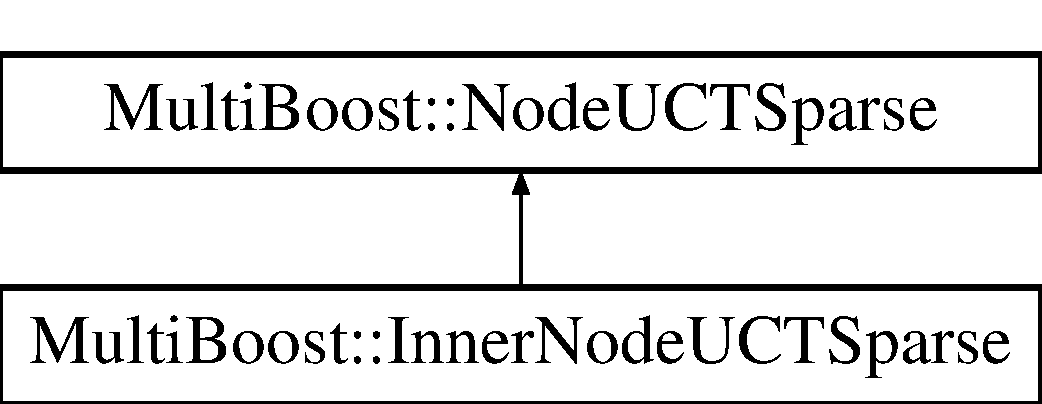
\includegraphics[height=2.000000cm]{classMultiBoost_1_1InnerNodeUCTSparse}
\end{center}
\end{figure}
\subsection*{Public Member Functions}
\begin{DoxyCompactItemize}
\item 
\hypertarget{classMultiBoost_1_1InnerNodeUCTSparse_afb08a2656465679f145c46d7a5494902}{virtual bool {\bfseries is\-Leaf} ()}\label{classMultiBoost_1_1InnerNodeUCTSparse_afb08a2656465679f145c46d7a5494902}

\item 
\hypertarget{classMultiBoost_1_1InnerNodeUCTSparse_a263a5cf7f9687d97723a411153cc429c}{{\bfseries Inner\-Node\-U\-C\-T\-Sparse} (\hyperlink{classMultiBoost_1_1NodeUCTSparse}{Node\-U\-C\-T\-Sparse} $\ast$n)}\label{classMultiBoost_1_1InnerNodeUCTSparse_a263a5cf7f9687d97723a411153cc429c}

\item 
\hypertarget{classMultiBoost_1_1InnerNodeUCTSparse_aaaa23503a7b7d6b81c7df6088d607d41}{virtual void {\bfseries create\-Inner\-Node\-Child} (int num)}\label{classMultiBoost_1_1InnerNodeUCTSparse_aaaa23503a7b7d6b81c7df6088d607d41}

\item 
\hypertarget{classMultiBoost_1_1InnerNodeUCTSparse_a92c9d857b5d37181c7a7e9d1c80bb78a}{virtual void {\bfseries create\-Inner\-Node\-One\-Child} (int num)}\label{classMultiBoost_1_1InnerNodeUCTSparse_a92c9d857b5d37181c7a7e9d1c80bb78a}

\item 
\hypertarget{classMultiBoost_1_1InnerNodeUCTSparse_aef13450e3fedb6b3de4b8f5b3cc9ac27}{virtual void {\bfseries create\-Leaf\-Node\-Child} (int num)}\label{classMultiBoost_1_1InnerNodeUCTSparse_aef13450e3fedb6b3de4b8f5b3cc9ac27}

\item 
\hypertarget{classMultiBoost_1_1InnerNodeUCTSparse_ac0a5a2cccabb2b16fd334bc1fd7ef8dd}{virtual void {\bfseries create\-Leaf\-Node\-One\-Child} (int num)}\label{classMultiBoost_1_1InnerNodeUCTSparse_ac0a5a2cccabb2b16fd334bc1fd7ef8dd}

\item 
\hypertarget{classMultiBoost_1_1InnerNodeUCTSparse_a0f1e670bc0c37c1ed6965e5a61e8211f}{virtual void {\bfseries clear\-Inner\-Node\-Child} ()}\label{classMultiBoost_1_1InnerNodeUCTSparse_a0f1e670bc0c37c1ed6965e5a61e8211f}

\item 
\hypertarget{classMultiBoost_1_1InnerNodeUCTSparse_a211da9f3f79fab897258017bbc4ab594}{virtual bool {\bfseries has\-Ith\-Child} (int num)}\label{classMultiBoost_1_1InnerNodeUCTSparse_a211da9f3f79fab897258017bbc4ab594}

\item 
\hypertarget{classMultiBoost_1_1InnerNodeUCTSparse_a41f9a0c2e728d014aa5c47f13b66d2f1}{virtual \hyperlink{classMultiBoost_1_1NodeUCTSparse}{Node\-U\-C\-T\-Sparse} $\ast$ {\bfseries getith\-Child} (int num)}\label{classMultiBoost_1_1InnerNodeUCTSparse_a41f9a0c2e728d014aa5c47f13b66d2f1}

\item 
\hypertarget{classMultiBoost_1_1InnerNodeUCTSparse_ac6084be399608cb1bf1f8d8711d5a159}{virtual int {\bfseries get\-Num\-Of\-Child} ()}\label{classMultiBoost_1_1InnerNodeUCTSparse_ac6084be399608cb1bf1f8d8711d5a159}

\item 
\hypertarget{classMultiBoost_1_1InnerNodeUCTSparse_aa3992af18473a2f7d9053834522b8181}{virtual void {\bfseries create\-Recursive\-U\-C\-T\-Tree} (int depth, int num\-Of\-Childs)}\label{classMultiBoost_1_1InnerNodeUCTSparse_aa3992af18473a2f7d9053834522b8181}

\item 
\hypertarget{classMultiBoost_1_1InnerNodeUCTSparse_a8e92241ea5a33183e811d649e9747f2e}{virtual void {\bfseries set\-Children\-Num} ()}\label{classMultiBoost_1_1InnerNodeUCTSparse_a8e92241ea5a33183e811d649e9747f2e}

\item 
\hypertarget{classMultiBoost_1_1InnerNodeUCTSparse_ab0c394361cb78bfcba06a22be08ef5eb}{virtual void {\bfseries clear\-Recursive\-U\-C\-T\-Tree} ()}\label{classMultiBoost_1_1InnerNodeUCTSparse_ab0c394361cb78bfcba06a22be08ef5eb}

\item 
\hypertarget{classMultiBoost_1_1InnerNodeUCTSparse_a87937be9c0e19fe6f4364e6104efd7a3}{virtual int {\bfseries get\-Child\-Ind\-With\-Max\-Bi} ()}\label{classMultiBoost_1_1InnerNodeUCTSparse_a87937be9c0e19fe6f4364e6104efd7a3}

\item 
\hypertarget{classMultiBoost_1_1InnerNodeUCTSparse_a76c4343f9ecc6a10f9ac55fe20536239}{virtual void {\bfseries get\-Best\-Trajectory} (vector$<$ int $>$ \&trajectory)}\label{classMultiBoost_1_1InnerNodeUCTSparse_a76c4343f9ecc6a10f9ac55fe20536239}

\item 
\hypertarget{classMultiBoost_1_1InnerNodeUCTSparse_a424624e87564a71ab8a7fc94a71f804b}{void {\bfseries update\-Inner\-Nodes} (double update\-Value, vector$<$ int $>$ \&trajectory)}\label{classMultiBoost_1_1InnerNodeUCTSparse_a424624e87564a71ab8a7fc94a71f804b}

\end{DoxyCompactItemize}
\subsection*{Protected Attributes}
\begin{DoxyCompactItemize}
\item 
\hypertarget{classMultiBoost_1_1InnerNodeUCTSparse_abf7677cc37a994e73ff66bb4e7531ae4}{vector$<$ \hyperlink{classMultiBoost_1_1NodeUCTSparse}{Node\-U\-C\-T\-Sparse} $\ast$ $>$ {\bfseries \-\_\-children}}\label{classMultiBoost_1_1InnerNodeUCTSparse_abf7677cc37a994e73ff66bb4e7531ae4}

\end{DoxyCompactItemize}
\subsection*{Additional Inherited Members}


\subsection{Detailed Description}


Definition at line 133 of file U\-C\-Tutils.\-h.



The documentation for this class was generated from the following file\-:\begin{DoxyCompactItemize}
\item 
C\-:/\-Users/fradav/\-Documents/\-Dev/\-C++/\-Multiboost/\-Sources/src/\-Utils/U\-C\-Tutils.\-h\end{DoxyCompactItemize}

\hypertarget{classMultiBoost_1_1InnerPoint}{
\section{MultiBoost::InnerPoint Class Reference}
\label{classMultiBoost_1_1InnerPoint}\index{MultiBoost::InnerPoint@{MultiBoost::InnerPoint}}
}


\subsection{Detailed Description}


Definition at line 68 of file TreeLearnerUCT.h.



The documentation for this class was generated from the following file:\begin{DoxyCompactItemize}
\item 
/cygdrive/c/Users/fradav/Documents/Dev/Multiboost/Sources/src/WeakLearners/\hyperlink{TreeLearnerUCT_8h}{TreeLearnerUCT.h}\end{DoxyCompactItemize}

\hypertarget{classMultiBoost_1_1InputData}{\section{Multi\-Boost\-:\-:Input\-Data Class Reference}
\label{classMultiBoost_1_1InputData}\index{Multi\-Boost\-::\-Input\-Data@{Multi\-Boost\-::\-Input\-Data}}
}


{\ttfamily \#include $<$Input\-Data.\-h$>$}

Inheritance diagram for Multi\-Boost\-:\-:Input\-Data\-:\begin{figure}[H]
\begin{center}
\leavevmode
\includegraphics[height=1.794872cm]{classMultiBoost_1_1InputData}
\end{center}
\end{figure}
\subsection*{Public Member Functions}
\begin{DoxyCompactItemize}
\item 
\hyperlink{classMultiBoost_1_1InputData_a98a5fea89a121fbc3a5a1727b5e3a4de}{Input\-Data} ()
\item 
\hypertarget{classMultiBoost_1_1InputData_aa4ea74f2c82341dac7caa7dc003b2010}{virtual int {\bfseries get\-Order\-Based\-On\-Raw\-Index} (int raw\-Index)}\label{classMultiBoost_1_1InputData_aa4ea74f2c82341dac7caa7dc003b2010}

\item 
\hypertarget{classMultiBoost_1_1InputData_a3ac4dab9bd669a63b7d32eb3fd315ae6}{virtual bool {\bfseries is\-Samples\-From\-One\-Class} ()}\label{classMultiBoost_1_1InputData_a3ac4dab9bd669a63b7d32eb3fd315ae6}

\item 
virtual void \hyperlink{classMultiBoost_1_1InputData_a2fb71a41b408568bf3f64dad6e457c34}{init\-Options} (const \hyperlink{classnor__utils_1_1Args}{nor\-\_\-utils\-::\-Args} \&args)
\item 
virtual void \hyperlink{classMultiBoost_1_1InputData_abf6290345aa3ffc9f81af71c41487390}{load} (const string \&file\-Name, e\-Input\-Type input\-Type=I\-T\-\_\-\-T\-R\-A\-I\-N, int verbose\-Level=1)
\item 
const vector$<$ \hyperlink{structMultiBoost_1_1Label}{Label} $>$ \& \hyperlink{classMultiBoost_1_1InputData_a0a1038757e7120197aab365e5c031b22}{get\-Labels} (const int idx) const 
\item 
\hypertarget{classMultiBoost_1_1InputData_a4ec7b1d8075c8e132393e716bdb12684}{vector$<$ \hyperlink{structMultiBoost_1_1Label}{Label} $>$ \& {\bfseries get\-Labels} (const int idx)}\label{classMultiBoost_1_1InputData_a4ec7b1d8075c8e132393e716bdb12684}

\item 
\hypertarget{classMultiBoost_1_1InputData_af5a2f8877cfa3928b814b0016025dac4}{const bool {\bfseries has\-Label} (const int idx, const int label\-Idx) const }\label{classMultiBoost_1_1InputData_af5a2f8877cfa3928b814b0016025dac4}

\item 
\hypertarget{classMultiBoost_1_1InputData_a6fd2dc4fd0187c3fa886348fbbe210e9}{const bool {\bfseries has\-Positive\-Label} (const int idx, const int label\-Idx) const }\label{classMultiBoost_1_1InputData_a6fd2dc4fd0187c3fa886348fbbe210e9}

\item 
const vector$<$ \hyperlink{Defaults_8h_a3a11cfe6a5d469d921716ca6291e934f}{Feature\-Real} $>$ \& \hyperlink{classMultiBoost_1_1InputData_aa2d6993a95e26c1c42ba329ef7088605}{get\-Values} (int idx) const 
\item 
\hypertarget{classMultiBoost_1_1InputData_a16a95b72d8df50d89af377b69c9bdc2a}{vector$<$ \hyperlink{Defaults_8h_a3a11cfe6a5d469d921716ca6291e934f}{Feature\-Real} $>$ \& {\bfseries get\-Values} (int idx)}\label{classMultiBoost_1_1InputData_a16a95b72d8df50d89af377b69c9bdc2a}

\item 
\hypertarget{classMultiBoost_1_1InputData_afea5f78e67045a871aca30ebf2570b11}{\hyperlink{Defaults_8h_a3a11cfe6a5d469d921716ca6291e934f}{Feature\-Real} {\bfseries get\-Value} (int idx, int column\-Idx) const }\label{classMultiBoost_1_1InputData_afea5f78e67045a871aca30ebf2570b11}

\item 
\hypertarget{classMultiBoost_1_1InputData_a787228eaef1f39bb2d01eee4edcc980a}{const \hyperlink{classMultiBoost_1_1Example}{Example} \& {\bfseries get\-Example} (int idx)}\label{classMultiBoost_1_1InputData_a787228eaef1f39bb2d01eee4edcc980a}

\item 
\hypertarget{classMultiBoost_1_1InputData_abd7168f1afd96c47be841cea8f2989e5}{virtual const vector$<$ \hyperlink{classMultiBoost_1_1Example}{Example} $>$ \& {\bfseries get\-Examples} ()}\label{classMultiBoost_1_1InputData_abd7168f1afd96c47be841cea8f2989e5}

\item 
\hypertarget{classMultiBoost_1_1InputData_a6026b56cdf91b87bf4e34455bdacf109}{const \hyperlink{classMultiBoost_1_1NameMap}{Name\-Map} \& {\bfseries get\-Class\-Map} ()}\label{classMultiBoost_1_1InputData_a6026b56cdf91b87bf4e34455bdacf109}

\item 
\hypertarget{classMultiBoost_1_1InputData_adf4637c0991eb39141636e8913d46371}{const \hyperlink{classMultiBoost_1_1NameMap}{Name\-Map} \& {\bfseries get\-Attribute\-Name\-Map} ()}\label{classMultiBoost_1_1InputData_adf4637c0991eb39141636e8913d46371}

\item 
\hypertarget{classMultiBoost_1_1InputData_abddf56997116900eca1ef6ef0da92b9d}{const \hyperlink{classMultiBoost_1_1NameMap}{Name\-Map} \& {\bfseries get\-Enum\-Map} (int j)}\label{classMultiBoost_1_1InputData_abddf56997116900eca1ef6ef0da92b9d}

\item 
const string \& \hyperlink{classMultiBoost_1_1InputData_a64d12c14b0f69c05b904bd809faabfb8}{get\-Example\-Name} (const int idx)
\item 
\hypertarget{classMultiBoost_1_1InputData_a96ab72ee9f4f3713786794cb4ae0b926}{int \hyperlink{classMultiBoost_1_1InputData_a96ab72ee9f4f3713786794cb4ae0b926}{get\-Num\-Attributes} () const }\label{classMultiBoost_1_1InputData_a96ab72ee9f4f3713786794cb4ae0b926}

\begin{DoxyCompactList}\small\item\em Returns the number of attributes. \end{DoxyCompactList}\item 
\hypertarget{classMultiBoost_1_1InputData_a6bbe9949016d04c361640c3624f9a32a}{int \hyperlink{classMultiBoost_1_1InputData_a6bbe9949016d04c361640c3624f9a32a}{get\-Num\-Examples} () const }\label{classMultiBoost_1_1InputData_a6bbe9949016d04c361640c3624f9a32a}

\begin{DoxyCompactList}\small\item\em Returns the number of examples. \end{DoxyCompactList}\item 
\hypertarget{classMultiBoost_1_1InputData_a389983328bd80477caa3885ed9830ff8}{int \hyperlink{classMultiBoost_1_1InputData_a389983328bd80477caa3885ed9830ff8}{get\-Num\-Classes} () const }\label{classMultiBoost_1_1InputData_a389983328bd80477caa3885ed9830ff8}

\begin{DoxyCompactList}\small\item\em Returns the number of classes. \end{DoxyCompactList}\item 
int \hyperlink{classMultiBoost_1_1InputData_adeeb05a894b4d7bf769d3d5c346006a7}{get\-Num\-Examples\-Per\-Class} (int class\-Idx) const 
\item 
\hypertarget{classMultiBoost_1_1InputData_a220bc98fc4f4935e71eef90d7f529655}{vector$<$ \hyperlink{Defaults_8h_a3a11cfe6a5d469d921716ca6291e934f}{Feature\-Real} $>$ \& {\bfseries get\-Most\-Frequent\-Value\-Per\-Feature} ()}\label{classMultiBoost_1_1InputData_a220bc98fc4f4935e71eef90d7f529655}

\item 
virtual int \hyperlink{classMultiBoost_1_1InputData_a00150efbaf1e3e994786ec1fb9283119}{load\-Index\-Set} (set$<$ int $>$ ind)
\item 
\hypertarget{classMultiBoost_1_1InputData_a9009df0e64b117bba2c1678039308279}{virtual void {\bfseries get\-Index\-Set} (set$<$ int $>$ \&ind)}\label{classMultiBoost_1_1InputData_a9009df0e64b117bba2c1678039308279}

\item 
void \hyperlink{classMultiBoost_1_1InputData_a536ee10e7bce2c4e707bcca105f2e06a}{clear\-Index\-Set} (void)
\item 
\hypertarget{classMultiBoost_1_1InputData_acb3b302a101c7a516992b2872d37b007}{bool {\bfseries is\-Filtered} ()}\label{classMultiBoost_1_1InputData_acb3b302a101c7a516992b2872d37b007}

\item 
\hypertarget{classMultiBoost_1_1InputData_a0c69adf7c58ff5f209d8a20563e16b21}{int {\bfseries get\-Raw\-Index} (int i)}\label{classMultiBoost_1_1InputData_a0c69adf7c58ff5f209d8a20563e16b21}

\item 
\hypertarget{classMultiBoost_1_1InputData_ac19367561e1476b37fd1d77d704e5f9f}{bool {\bfseries is\-Used\-Indice} (int x)}\label{classMultiBoost_1_1InputData_ac19367561e1476b37fd1d77d704e5f9f}

\item 
\hypertarget{classMultiBoost_1_1InputData_adfa7715d0a56617c4929cd41980b9f82}{\hyperlink{Defaults_8h_a3a11cfe6a5d469d921716ca6291e934f}{Feature\-Real} {\bfseries get\-Featurewise\-Max} (int idx)}\label{classMultiBoost_1_1InputData_adfa7715d0a56617c4929cd41980b9f82}

\item 
\hypertarget{classMultiBoost_1_1InputData_a37caf81e5da1ea2bfbdd20b8a045a1f8}{\hyperlink{Defaults_8h_a3a11cfe6a5d469d921716ca6291e934f}{Feature\-Real} {\bfseries get\-Featurewise\-Min} (int idx)}\label{classMultiBoost_1_1InputData_a37caf81e5da1ea2bfbdd20b8a045a1f8}

\item 
\hypertarget{classMultiBoost_1_1InputData_ac8045d1da75924f8e4186a3fe54841d7}{void {\bfseries add\-Example} (\hyperlink{classMultiBoost_1_1Example}{Example} example)}\label{classMultiBoost_1_1InputData_ac8045d1da75924f8e4186a3fe54841d7}

\end{DoxyCompactItemize}
\subsection*{Protected Attributes}
\begin{DoxyCompactItemize}
\item 
\hypertarget{classMultiBoost_1_1InputData_a7e2ce350ff087bd432d68284af8497f8}{bool {\bfseries \-\_\-has\-Example\-Name}}\label{classMultiBoost_1_1InputData_a7e2ce350ff087bd432d68284af8497f8}

\item 
\hypertarget{classMultiBoost_1_1InputData_a804172ec7b0847a4219d2835d12686f0}{bool {\bfseries \-\_\-class\-In\-Last\-Column}}\label{classMultiBoost_1_1InputData_a804172ec7b0847a4219d2835d12686f0}

\item 
\hypertarget{classMultiBoost_1_1InputData_a8382cb85fea970f166dccced6fd1ce6c}{vector$<$ int $>$ {\bfseries \-\_\-indirect\-Indices}}\label{classMultiBoost_1_1InputData_a8382cb85fea970f166dccced6fd1ce6c}

\item 
\hypertarget{classMultiBoost_1_1InputData_acb73416ea99f100ec3affba72c41b19b}{vector$<$ int $>$ {\bfseries \-\_\-raw\-Indices}}\label{classMultiBoost_1_1InputData_acb73416ea99f100ec3affba72c41b19b}

\item 
\hypertarget{classMultiBoost_1_1InputData_a7266ca3c43c683ad928e1fefdf6a2504}{bool {\bfseries \-\_\-subset\-Already\-Computed}}\label{classMultiBoost_1_1InputData_a7266ca3c43c683ad928e1fefdf6a2504}

\item 
\hypertarget{classMultiBoost_1_1InputData_a1e68d0fda0476f676224dbc5a1291250}{int \hyperlink{classMultiBoost_1_1InputData_a1e68d0fda0476f676224dbc5a1291250}{\-\_\-num\-Examples}}\label{classMultiBoost_1_1InputData_a1e68d0fda0476f676224dbc5a1291250}

\begin{DoxyCompactList}\small\item\em The number of examples. \end{DoxyCompactList}\item 
\hypertarget{classMultiBoost_1_1InputData_a318fdc8f828b5ea291a25397f03d8232}{vector$<$ int $>$ \hyperlink{classMultiBoost_1_1InputData_a318fdc8f828b5ea291a25397f03d8232}{\-\_\-n\-Examples\-Per\-Class}}\label{classMultiBoost_1_1InputData_a318fdc8f828b5ea291a25397f03d8232}

\begin{DoxyCompactList}\small\item\em The number of examples per class. \end{DoxyCompactList}\item 
\hypertarget{classMultiBoost_1_1InputData_a0c77a5e26b5231352560f631afdd24da}{\hyperlink{classMultiBoost_1_1RawData}{Raw\-Data} $\ast$ {\bfseries \-\_\-p\-Data}}\label{classMultiBoost_1_1InputData_a0c77a5e26b5231352560f631afdd24da}

\item 
\hypertarget{classMultiBoost_1_1InputData_affb60cdf419808ed8af1861a4c5f8b8d}{vector$<$ \hyperlink{classMultiBoost_1_1Example}{Example} $>$ {\bfseries \-\_\-subset}}\label{classMultiBoost_1_1InputData_affb60cdf419808ed8af1861a4c5f8b8d}

\end{DoxyCompactItemize}


\subsection{Detailed Description}
Handles the data. This class not just holds the data information but also the weights on examples and labels. It also stores the sorted data (for decision stump algorithms) if necessary.

\begin{DoxyDate}{Date}
05/11/2005 
\end{DoxyDate}


Definition at line 82 of file Input\-Data.\-h.



\subsection{Constructor \& Destructor Documentation}
\hypertarget{classMultiBoost_1_1InputData_a98a5fea89a121fbc3a5a1727b5e3a4de}{\index{Multi\-Boost\-::\-Input\-Data@{Multi\-Boost\-::\-Input\-Data}!Input\-Data@{Input\-Data}}
\index{Input\-Data@{Input\-Data}!MultiBoost::InputData@{Multi\-Boost\-::\-Input\-Data}}
\subsubsection[{Input\-Data}]{\setlength{\rightskip}{0pt plus 5cm}Multi\-Boost\-::\-Input\-Data\-::\-Input\-Data (
\begin{DoxyParamCaption}
{}
\end{DoxyParamCaption}
)\hspace{0.3cm}{\ttfamily [inline]}}}\label{classMultiBoost_1_1InputData_a98a5fea89a121fbc3a5a1727b5e3a4de}
The constructor. It does noting but initializing some variables. \begin{DoxyDate}{Date}
12/11/2005 
\end{DoxyDate}


Definition at line 102 of file Input\-Data.\-h.



\subsection{Member Function Documentation}
\hypertarget{classMultiBoost_1_1InputData_a536ee10e7bce2c4e707bcca105f2e06a}{\index{Multi\-Boost\-::\-Input\-Data@{Multi\-Boost\-::\-Input\-Data}!clear\-Index\-Set@{clear\-Index\-Set}}
\index{clear\-Index\-Set@{clear\-Index\-Set}!MultiBoost::InputData@{Multi\-Boost\-::\-Input\-Data}}
\subsubsection[{clear\-Index\-Set}]{\setlength{\rightskip}{0pt plus 5cm}void Multi\-Boost\-::\-Input\-Data\-::clear\-Index\-Set (
\begin{DoxyParamCaption}
\item[{void}]{}
\end{DoxyParamCaption}
)}}\label{classMultiBoost_1_1InputData_a536ee10e7bce2c4e707bcca105f2e06a}
Clear the indices of subset we use, the whole dataset containing \-\_\-p\-Data will be used
\begin{DoxyItemize}
\item 12/10/2009 
\end{DoxyItemize}

Definition at line 131 of file Input\-Data.\-cpp.

\hypertarget{classMultiBoost_1_1InputData_a64d12c14b0f69c05b904bd809faabfb8}{\index{Multi\-Boost\-::\-Input\-Data@{Multi\-Boost\-::\-Input\-Data}!get\-Example\-Name@{get\-Example\-Name}}
\index{get\-Example\-Name@{get\-Example\-Name}!MultiBoost::InputData@{Multi\-Boost\-::\-Input\-Data}}
\subsubsection[{get\-Example\-Name}]{\setlength{\rightskip}{0pt plus 5cm}const string\& Multi\-Boost\-::\-Input\-Data\-::get\-Example\-Name (
\begin{DoxyParamCaption}
\item[{const int}]{idx}
\end{DoxyParamCaption}
)\hspace{0.3cm}{\ttfamily [inline]}}}\label{classMultiBoost_1_1InputData_a64d12c14b0f69c05b904bd809faabfb8}
Get the label of the example. 
\begin{DoxyParams}{Parameters}
{\em idx} & The index of the example. \\
\hline
\end{DoxyParams}
\begin{DoxyReturn}{Returns}
A string with the label of the example, if this has been specified with --examplename argument. 
\end{DoxyReturn}
\begin{DoxyDate}{Date}
14/2/2006 
\end{DoxyDate}


Definition at line 247 of file Input\-Data.\-h.

\hypertarget{classMultiBoost_1_1InputData_a0a1038757e7120197aab365e5c031b22}{\index{Multi\-Boost\-::\-Input\-Data@{Multi\-Boost\-::\-Input\-Data}!get\-Labels@{get\-Labels}}
\index{get\-Labels@{get\-Labels}!MultiBoost::InputData@{Multi\-Boost\-::\-Input\-Data}}
\subsubsection[{get\-Labels}]{\setlength{\rightskip}{0pt plus 5cm}const vector$<${\bf Label}$>$\& Multi\-Boost\-::\-Input\-Data\-::get\-Labels (
\begin{DoxyParamCaption}
\item[{const int}]{idx}
\end{DoxyParamCaption}
) const\hspace{0.3cm}{\ttfamily [inline]}}}\label{classMultiBoost_1_1InputData_a0a1038757e7120197aab365e5c031b22}
Gets the labels of the given example. 
\begin{DoxyParams}{Parameters}
{\em idx} & The index of the example \\
\hline
\end{DoxyParams}
\begin{DoxyReturn}{Returns}
The labels of the example \mbox{[}idx\mbox{]}. 
\end{DoxyReturn}
\begin{DoxyDate}{Date}
10/11/2005 
\end{DoxyDate}


Definition at line 168 of file Input\-Data.\-h.

\hypertarget{classMultiBoost_1_1InputData_adeeb05a894b4d7bf769d3d5c346006a7}{\index{Multi\-Boost\-::\-Input\-Data@{Multi\-Boost\-::\-Input\-Data}!get\-Num\-Examples\-Per\-Class@{get\-Num\-Examples\-Per\-Class}}
\index{get\-Num\-Examples\-Per\-Class@{get\-Num\-Examples\-Per\-Class}!MultiBoost::InputData@{Multi\-Boost\-::\-Input\-Data}}
\subsubsection[{get\-Num\-Examples\-Per\-Class}]{\setlength{\rightskip}{0pt plus 5cm}int Multi\-Boost\-::\-Input\-Data\-::get\-Num\-Examples\-Per\-Class (
\begin{DoxyParamCaption}
\item[{int}]{class\-Idx}
\end{DoxyParamCaption}
) const\hspace{0.3cm}{\ttfamily [inline]}}}\label{classMultiBoost_1_1InputData_adeeb05a894b4d7bf769d3d5c346006a7}
Get the number of examples per class. 
\begin{DoxyParams}{Parameters}
{\em class\-Idx} & The index of the class. \\
\hline
\end{DoxyParams}
\begin{DoxyDate}{Date}
11/11/2005 
\end{DoxyDate}


Definition at line 260 of file Input\-Data.\-h.

\hypertarget{classMultiBoost_1_1InputData_aa2d6993a95e26c1c42ba329ef7088605}{\index{Multi\-Boost\-::\-Input\-Data@{Multi\-Boost\-::\-Input\-Data}!get\-Values@{get\-Values}}
\index{get\-Values@{get\-Values}!MultiBoost::InputData@{Multi\-Boost\-::\-Input\-Data}}
\subsubsection[{get\-Values}]{\setlength{\rightskip}{0pt plus 5cm}const vector$<${\bf Feature\-Real}$>$\& Multi\-Boost\-::\-Input\-Data\-::get\-Values (
\begin{DoxyParamCaption}
\item[{int}]{idx}
\end{DoxyParamCaption}
) const\hspace{0.3cm}{\ttfamily [inline]}}}\label{classMultiBoost_1_1InputData_aa2d6993a95e26c1c42ba329ef7088605}
Get the values of the example {\itshape idx} 
\begin{DoxyParams}{Parameters}
{\em idx} & The index of the example. \\
\hline
\end{DoxyParams}
\begin{DoxyDate}{Date}
11/11/2005 
\end{DoxyDate}


Definition at line 182 of file Input\-Data.\-h.

\hypertarget{classMultiBoost_1_1InputData_a2fb71a41b408568bf3f64dad6e457c34}{\index{Multi\-Boost\-::\-Input\-Data@{Multi\-Boost\-::\-Input\-Data}!init\-Options@{init\-Options}}
\index{init\-Options@{init\-Options}!MultiBoost::InputData@{Multi\-Boost\-::\-Input\-Data}}
\subsubsection[{init\-Options}]{\setlength{\rightskip}{0pt plus 5cm}virtual void Multi\-Boost\-::\-Input\-Data\-::init\-Options (
\begin{DoxyParamCaption}
\item[{const {\bf nor\-\_\-utils\-::\-Args} \&}]{args}
\end{DoxyParamCaption}
)\hspace{0.3cm}{\ttfamily [inline]}, {\ttfamily [virtual]}}}\label{classMultiBoost_1_1InputData_a2fb71a41b408568bf3f64dad6e457c34}
Set the arguments of the algorithm using the standard interface of the arguments. Call this to set the arguments asked by the user. 
\begin{DoxyParams}{Parameters}
{\em args} & The arguments defined by the user in the command line. on the derived classes. \\
\hline
\end{DoxyParams}
\begin{DoxyWarning}{Warning}
It does not have a declare\-Arguments because it is dealt by the weak learner responsible for the input data (so that the option goes under its own group). 
\end{DoxyWarning}
\begin{DoxyDate}{Date}
14/11/2005 
\end{DoxyDate}


Reimplemented in \hyperlink{classMultiBoost_1_1HaarData_a3b37aff7853230f715ab0ad62610ddbb}{Multi\-Boost\-::\-Haar\-Data}.



Definition at line 131 of file Input\-Data.\-h.

\hypertarget{classMultiBoost_1_1InputData_abf6290345aa3ffc9f81af71c41487390}{\index{Multi\-Boost\-::\-Input\-Data@{Multi\-Boost\-::\-Input\-Data}!load@{load}}
\index{load@{load}!MultiBoost::InputData@{Multi\-Boost\-::\-Input\-Data}}
\subsubsection[{load}]{\setlength{\rightskip}{0pt plus 5cm}virtual void Multi\-Boost\-::\-Input\-Data\-::load (
\begin{DoxyParamCaption}
\item[{const string \&}]{file\-Name, }
\item[{e\-Input\-Type}]{input\-Type = {\ttfamily IT\-\_\-TRAIN}, }
\item[{int}]{verbose\-Level = {\ttfamily 1}}
\end{DoxyParamCaption}
)\hspace{0.3cm}{\ttfamily [inline]}, {\ttfamily [virtual]}}}\label{classMultiBoost_1_1InputData_abf6290345aa3ffc9f81af71c41487390}
Load the given file. 
\begin{DoxyParams}{Parameters}
{\em file\-Name} & The name of the file to be loaded. \\
\hline
{\em input\-Type} & The type of input. \\
\hline
{\em verbose\-Level} & The level of verbosity. \\
\hline
\end{DoxyParams}
\begin{DoxySeeAlso}{See Also}
e\-Input\-Type 
\end{DoxySeeAlso}
\begin{DoxyDate}{Date}
08/11/2005 
\end{DoxyDate}


Reimplemented in \hyperlink{classMultiBoost_1_1HaarData_af48d9ca35effea8c6f653b66cfc81b71}{Multi\-Boost\-::\-Haar\-Data}, and \hyperlink{classMultiBoost_1_1SortedData_a4026ff8765982ac0c0edff12a929917f}{Multi\-Boost\-::\-Sorted\-Data}.



Definition at line 143 of file Input\-Data.\-h.

\hypertarget{classMultiBoost_1_1InputData_a00150efbaf1e3e994786ec1fb9283119}{\index{Multi\-Boost\-::\-Input\-Data@{Multi\-Boost\-::\-Input\-Data}!load\-Index\-Set@{load\-Index\-Set}}
\index{load\-Index\-Set@{load\-Index\-Set}!MultiBoost::InputData@{Multi\-Boost\-::\-Input\-Data}}
\subsubsection[{load\-Index\-Set}]{\setlength{\rightskip}{0pt plus 5cm}int Multi\-Boost\-::\-Input\-Data\-::load\-Index\-Set (
\begin{DoxyParamCaption}
\item[{set$<$ int $>$}]{ind}
\end{DoxyParamCaption}
)\hspace{0.3cm}{\ttfamily [virtual]}}}\label{classMultiBoost_1_1InputData_a00150efbaf1e3e994786ec1fb9283119}
Set the indices of subset we use 
\begin{DoxyParams}{Parameters}
{\em the} & set which contains the indices  12/10/2009 \\
\hline
\end{DoxyParams}


Definition at line 85 of file Input\-Data.\-cpp.



The documentation for this class was generated from the following files\-:\begin{DoxyCompactItemize}
\item 
C\-:/\-Users/fradav/\-Documents/\-Dev/\-C++/\-Multiboost/\-Sources/src/\-I\-O/\hyperlink{InputData_8h}{Input\-Data.\-h}\item 
C\-:/\-Users/fradav/\-Documents/\-Dev/\-C++/\-Multiboost/\-Sources/src/\-I\-O/Input\-Data.\-cpp\end{DoxyCompactItemize}

\hypertarget{structMultiBoost_1_1Label}{\section{Multi\-Boost\-:\-:Label Struct Reference}
\label{structMultiBoost_1_1Label}\index{Multi\-Boost\-::\-Label@{Multi\-Boost\-::\-Label}}
}
\subsection*{Public Member Functions}
\begin{DoxyCompactItemize}
\item 
\hypertarget{structMultiBoost_1_1Label_a7ad8bc948da90f12fcd395a34a32ea62}{{\bfseries Label} (int idx\-In, \hyperlink{Defaults_8h_a80184c4fd10ab70a1a17c5f97dcd1563}{Alpha\-Real} weight\-In, \hyperlink{Defaults_8h_a80184c4fd10ab70a1a17c5f97dcd1563}{Alpha\-Real} initial\-Weight\-In, char y\-In)}\label{structMultiBoost_1_1Label_a7ad8bc948da90f12fcd395a34a32ea62}

\item 
\hypertarget{structMultiBoost_1_1Label_a79f7a99332c6736a95e6dc07c948a3ee}{bool {\bfseries operator==} (const int idx) const }\label{structMultiBoost_1_1Label_a79f7a99332c6736a95e6dc07c948a3ee}

\end{DoxyCompactItemize}
\subsection*{Public Attributes}
\begin{DoxyCompactItemize}
\item 
\hypertarget{structMultiBoost_1_1Label_a6a672c3044b66e08b5fcda0fdfb573b8}{int {\bfseries idx}}\label{structMultiBoost_1_1Label_a6a672c3044b66e08b5fcda0fdfb573b8}

\item 
\hypertarget{structMultiBoost_1_1Label_af1ca51e30da1ca1df50fa1fa88fb5361}{\hyperlink{Defaults_8h_a80184c4fd10ab70a1a17c5f97dcd1563}{Alpha\-Real} {\bfseries weight}}\label{structMultiBoost_1_1Label_af1ca51e30da1ca1df50fa1fa88fb5361}

\item 
\hypertarget{structMultiBoost_1_1Label_a9755be02bff3c8c7f8172764fc391265}{\hyperlink{Defaults_8h_a80184c4fd10ab70a1a17c5f97dcd1563}{Alpha\-Real} {\bfseries initial\-Weight}}\label{structMultiBoost_1_1Label_a9755be02bff3c8c7f8172764fc391265}

\item 
\hypertarget{structMultiBoost_1_1Label_ac3b8392c495a1989dce97bd9a883f93b}{char {\bfseries y}}\label{structMultiBoost_1_1Label_ac3b8392c495a1989dce97bd9a883f93b}

\end{DoxyCompactItemize}


\subsection{Detailed Description}


Definition at line 80 of file Example.\-h.



The documentation for this struct was generated from the following file\-:\begin{DoxyCompactItemize}
\item 
C\-:/\-Users/fradav/\-Documents/\-Dev/\-C++/\-Multiboost/\-Sources/src/\-Others/\hyperlink{Example_8h}{Example.\-h}\end{DoxyCompactItemize}

\hypertarget{classMultiBoost_1_1LeafNodeSparse}{\section{Multi\-Boost\-:\-:Leaf\-Node\-Sparse Class Reference}
\label{classMultiBoost_1_1LeafNodeSparse}\index{Multi\-Boost\-::\-Leaf\-Node\-Sparse@{Multi\-Boost\-::\-Leaf\-Node\-Sparse}}
}
Inheritance diagram for Multi\-Boost\-:\-:Leaf\-Node\-Sparse\-:\begin{figure}[H]
\begin{center}
\leavevmode
\includegraphics[height=2.000000cm]{classMultiBoost_1_1LeafNodeSparse}
\end{center}
\end{figure}
\subsection*{Public Member Functions}
\begin{DoxyCompactItemize}
\item 
\hypertarget{classMultiBoost_1_1LeafNodeSparse_a0f6230f2790d0fbf138f47847144934c}{{\bfseries Leaf\-Node\-Sparse} (\hyperlink{classMultiBoost_1_1NodeUCTSparse}{Node\-U\-C\-T\-Sparse} $\ast$n)}\label{classMultiBoost_1_1LeafNodeSparse_a0f6230f2790d0fbf138f47847144934c}

\item 
\hypertarget{classMultiBoost_1_1LeafNodeSparse_a3c43c42444bb5d98c180dd73046cd9c2}{virtual bool {\bfseries is\-Leaf} ()}\label{classMultiBoost_1_1LeafNodeSparse_a3c43c42444bb5d98c180dd73046cd9c2}

\item 
\hypertarget{classMultiBoost_1_1LeafNodeSparse_a2217389896d7d05bf01b26d0ca5d89de}{virtual \hyperlink{classMultiBoost_1_1NodeUCTSparse}{Node\-U\-C\-T\-Sparse} $\ast$ {\bfseries getith\-Child} (int num)}\label{classMultiBoost_1_1LeafNodeSparse_a2217389896d7d05bf01b26d0ca5d89de}

\item 
\hypertarget{classMultiBoost_1_1LeafNodeSparse_a497746b8d995828b149138b578742ef5}{virtual void {\bfseries clear\-Inner\-Node\-Child} ()}\label{classMultiBoost_1_1LeafNodeSparse_a497746b8d995828b149138b578742ef5}

\item 
\hypertarget{classMultiBoost_1_1LeafNodeSparse_a7debf95f7d215bb43bddbf13f235686f}{virtual int {\bfseries get\-Num\-Of\-Child} ()}\label{classMultiBoost_1_1LeafNodeSparse_a7debf95f7d215bb43bddbf13f235686f}

\item 
\hypertarget{classMultiBoost_1_1LeafNodeSparse_a79c0ad0990b997f75b36b60daae22a1d}{virtual int {\bfseries get\-Child\-Ind\-With\-Max\-Bi} ()}\label{classMultiBoost_1_1LeafNodeSparse_a79c0ad0990b997f75b36b60daae22a1d}

\end{DoxyCompactItemize}
\subsection*{Additional Inherited Members}


\subsection{Detailed Description}


Definition at line 117 of file U\-C\-Tutils.\-h.



The documentation for this class was generated from the following file\-:\begin{DoxyCompactItemize}
\item 
C\-:/\-Users/fradav/\-Documents/\-Dev/\-C++/\-Multiboost/\-Sources/src/\-Utils/U\-C\-Tutils.\-h\end{DoxyCompactItemize}

\hypertarget{classMultiBoost_1_1MAEOuput}{\section{Multi\-Boost\-:\-:M\-A\-E\-Ouput Class Reference}
\label{classMultiBoost_1_1MAEOuput}\index{Multi\-Boost\-::\-M\-A\-E\-Ouput@{Multi\-Boost\-::\-M\-A\-E\-Ouput}}
}


{\ttfamily \#include $<$Output\-Info.\-h$>$}

Inheritance diagram for Multi\-Boost\-:\-:M\-A\-E\-Ouput\-:\begin{figure}[H]
\begin{center}
\leavevmode
\includegraphics[height=2.000000cm]{classMultiBoost_1_1MAEOuput}
\end{center}
\end{figure}
\subsection*{Public Member Functions}
\begin{DoxyCompactItemize}
\item 
void \hyperlink{classMultiBoost_1_1MAEOuput_aea5df1d89f3ea04e20c5b7c2b4604d72}{output\-Header} (ostream \&out\-Stream, const \hyperlink{classMultiBoost_1_1NameMap}{Name\-Map} \&namemap)
\item 
void \hyperlink{classMultiBoost_1_1MAEOuput_a6583e24280a47504100247cc749fc44b}{output\-Description} (ostream \&out\-Stream)
\item 
\hypertarget{classMultiBoost_1_1MAEOuput_ae0af6a24dc60c56c236382b02fb52153}{void {\bfseries compute\-And\-Output} (ostream \&out\-Stream, \hyperlink{classMultiBoost_1_1InputData}{Input\-Data} $\ast$p\-Data, map$<$ \hyperlink{classMultiBoost_1_1InputData}{Input\-Data} $\ast$, table $>$ \&g\-Table\-Map, map$<$ \hyperlink{classMultiBoost_1_1InputData}{Input\-Data} $\ast$, table $>$ \&margins\-Table\-Map, map$<$ \hyperlink{classMultiBoost_1_1InputData}{Input\-Data} $\ast$, \hyperlink{Defaults_8h_a80184c4fd10ab70a1a17c5f97dcd1563}{Alpha\-Real} $>$ \&alpha\-Sums, \hyperlink{classMultiBoost_1_1BaseLearner}{Base\-Learner} $\ast$p\-Weak\-Hypothesis=0)}\label{classMultiBoost_1_1MAEOuput_ae0af6a24dc60c56c236382b02fb52153}

\end{DoxyCompactItemize}
\subsection*{Additional Inherited Members}


\subsection{Detailed Description}
M\-A\-E \begin{DoxyDate}{Date}
20/06/2011 
\end{DoxyDate}


Definition at line 663 of file Output\-Info.\-h.



\subsection{Member Function Documentation}
\hypertarget{classMultiBoost_1_1MAEOuput_a6583e24280a47504100247cc749fc44b}{\index{Multi\-Boost\-::\-M\-A\-E\-Ouput@{Multi\-Boost\-::\-M\-A\-E\-Ouput}!output\-Description@{output\-Description}}
\index{output\-Description@{output\-Description}!MultiBoost::MAEOuput@{Multi\-Boost\-::\-M\-A\-E\-Ouput}}
\subsubsection[{output\-Description}]{\setlength{\rightskip}{0pt plus 5cm}void Multi\-Boost\-::\-M\-A\-E\-Ouput\-::output\-Description (
\begin{DoxyParamCaption}
\item[{ostream \&}]{out\-Stream}
\end{DoxyParamCaption}
)\hspace{0.3cm}{\ttfamily [inline]}, {\ttfamily [virtual]}}}\label{classMultiBoost_1_1MAEOuput_a6583e24280a47504100247cc749fc44b}
Print a detailed description of the output. 
\begin{DoxyParams}{Parameters}
{\em out\-Stream} & The stream where the output is directed to \\
\hline
\end{DoxyParams}
\begin{DoxyDate}{Date}
12/12/2012 
\end{DoxyDate}


Reimplemented from \hyperlink{classMultiBoost_1_1BaseOutputInfoType_aa2f886100b21c8cf09d5dddc9e4d1dca}{Multi\-Boost\-::\-Base\-Output\-Info\-Type}.



Definition at line 671 of file Output\-Info.\-h.

\hypertarget{classMultiBoost_1_1MAEOuput_aea5df1d89f3ea04e20c5b7c2b4604d72}{\index{Multi\-Boost\-::\-M\-A\-E\-Ouput@{Multi\-Boost\-::\-M\-A\-E\-Ouput}!output\-Header@{output\-Header}}
\index{output\-Header@{output\-Header}!MultiBoost::MAEOuput@{Multi\-Boost\-::\-M\-A\-E\-Ouput}}
\subsubsection[{output\-Header}]{\setlength{\rightskip}{0pt plus 5cm}void Multi\-Boost\-::\-M\-A\-E\-Ouput\-::output\-Header (
\begin{DoxyParamCaption}
\item[{ostream \&}]{out\-Stream, }
\item[{const {\bf Name\-Map} \&}]{namemap}
\end{DoxyParamCaption}
)\hspace{0.3cm}{\ttfamily [inline]}, {\ttfamily [virtual]}}}\label{classMultiBoost_1_1MAEOuput_aea5df1d89f3ea04e20c5b7c2b4604d72}
Print the header 
\begin{DoxyParams}{Parameters}
{\em out\-Stream} & The stream where the output is directed to \\
\hline
{\em namemap} & The structure that contains the class information ( \\
\hline
\end{DoxyParams}
\begin{DoxySeeAlso}{See Also}
\hyperlink{classMultiBoost_1_1NameMap}{Name\-Map} ) 
\end{DoxySeeAlso}
\begin{DoxyDate}{Date}
17/06/2011 
\end{DoxyDate}


Implements \hyperlink{classMultiBoost_1_1BaseOutputInfoType_aec8678cadeec12db720af8b482c63662}{Multi\-Boost\-::\-Base\-Output\-Info\-Type}.



Definition at line 667 of file Output\-Info.\-h.



The documentation for this class was generated from the following files\-:\begin{DoxyCompactItemize}
\item 
C\-:/\-Users/fradav/\-Documents/\-Dev/\-C++/\-Multiboost/\-Sources/src/\-I\-O/\hyperlink{OutputInfo_8h}{Output\-Info.\-h}\item 
C\-:/\-Users/fradav/\-Documents/\-Dev/\-C++/\-Multiboost/\-Sources/src/\-I\-O/Output\-Info.\-cpp\end{DoxyCompactItemize}

\input{classMultiBoost_1_1MarginsOutput}
\hypertarget{classMultiBoost_1_1MultiStumpLearner}{
\section{MultiBoost::MultiStumpLearner Class Reference}
\label{classMultiBoost_1_1MultiStumpLearner}\index{MultiBoost::MultiStumpLearner@{MultiBoost::MultiStumpLearner}}
}


{\ttfamily \#include $<$MultiStumpLearner.h$>$}

Inheritance diagram for MultiBoost::MultiStumpLearner:\begin{figure}[H]
\begin{center}
\leavevmode
\includegraphics[height=4.000000cm]{classMultiBoost_1_1MultiStumpLearner}
\end{center}
\end{figure}
\subsection*{Public Member Functions}
\begin{DoxyCompactItemize}
\item 
\hyperlink{classMultiBoost_1_1MultiStumpLearner_a640b74072333a3c523db636e916a9f50}{MultiStumpLearner} ()
\item 
virtual \hyperlink{classMultiBoost_1_1MultiStumpLearner_a2d64a523c1a2f76c6d788948c5914bd3}{$\sim$MultiStumpLearner} ()
\item 
virtual \hyperlink{classMultiBoost_1_1BaseLearner}{BaseLearner} $\ast$ \hyperlink{classMultiBoost_1_1MultiStumpLearner_a2a3c04efd1a250269a741ee83d11d988}{subCreate} ()
\item 
virtual \hyperlink{classMultiBoost_1_1InputData}{InputData} $\ast$ \hyperlink{classMultiBoost_1_1MultiStumpLearner_a62763cd19797a15161ef3134d7b8acc8}{createInputData} ()
\item 
virtual \hyperlink{Defaults_8h_a80184c4fd10ab70a1a17c5f97dcd1563}{AlphaReal} \hyperlink{classMultiBoost_1_1MultiStumpLearner_a682f5428b73db0e89de8128539108f6b}{run} ()
\item 
virtual void \hyperlink{classMultiBoost_1_1MultiStumpLearner_a61d17e2ac24c475f7d11e03abcb2e1de}{declareArguments} (\hyperlink{classnor__utils_1_1Args}{nor\_\-utils::Args} \&args)
\item 
virtual void \hyperlink{classMultiBoost_1_1MultiStumpLearner_a5fe30fa4df79be1937eae9341a96a320}{initLearningOptions} (const \hyperlink{classnor__utils_1_1Args}{nor\_\-utils::Args} \&args)
\item 
virtual void \hyperlink{classMultiBoost_1_1MultiStumpLearner_a1677eba09a926f5a27570506b117f3d1}{save} (ofstream \&outputStream, int numTabs=0)
\item 
virtual void \hyperlink{classMultiBoost_1_1MultiStumpLearner_a5fea1fcb77fb6372ee4ed57fcfa8867b}{load} (\hyperlink{classnor__utils_1_1StreamTokenizer}{nor\_\-utils::StreamTokenizer} \&st)
\item 
virtual void \hyperlink{classMultiBoost_1_1MultiStumpLearner_a261fe1a54a6032f23759c4287afe39e3}{subCopyState} (\hyperlink{classMultiBoost_1_1BaseLearner}{BaseLearner} $\ast$pBaseLearner)
\end{DoxyCompactItemize}
\subsection*{Protected Member Functions}
\begin{DoxyCompactItemize}
\item 
virtual \hyperlink{Defaults_8h_a80184c4fd10ab70a1a17c5f97dcd1563}{AlphaReal} \hyperlink{classMultiBoost_1_1MultiStumpLearner_a5ccf4057af3064e833ae8da920e29d42}{phi} (\hyperlink{classMultiBoost_1_1InputData}{InputData} $\ast$pData, int idx, int classIdx) const 
\item 
virtual \hyperlink{Defaults_8h_a80184c4fd10ab70a1a17c5f97dcd1563}{AlphaReal} \hyperlink{classMultiBoost_1_1MultiStumpLearner_aec2e42f65f07886a4c3969d1d79f0c18}{phi} (\hyperlink{Defaults_8h_a3a11cfe6a5d469d921716ca6291e934f}{FeatureReal} val, int classIdx) const 
\end{DoxyCompactItemize}
\subsection*{Protected Attributes}
\begin{DoxyCompactItemize}
\item 
\hypertarget{classMultiBoost_1_1MultiStumpLearner_adf516324abf54cc94bed0c1be974e416}{
vector$<$ int $>$ {\bfseries \_\-selectedColumnArray}}
\label{classMultiBoost_1_1MultiStumpLearner_adf516324abf54cc94bed0c1be974e416}

\item 
\hypertarget{classMultiBoost_1_1MultiStumpLearner_aad761ccec4f51efa49261dc83d0c404f}{
vector$<$ \hyperlink{Defaults_8h_a3a11cfe6a5d469d921716ca6291e934f}{FeatureReal} $>$ \hyperlink{classMultiBoost_1_1MultiStumpLearner_aad761ccec4f51efa49261dc83d0c404f}{\_\-thresholds}}
\label{classMultiBoost_1_1MultiStumpLearner_aad761ccec4f51efa49261dc83d0c404f}

\begin{DoxyCompactList}\small\item\em The thresholds (one for each class) of the decision stump. \end{DoxyCompactList}\item 
\hypertarget{classMultiBoost_1_1MultiStumpLearner_a4091d825332ef577f2b2a64cf8feee82}{
int \hyperlink{classMultiBoost_1_1MultiStumpLearner_a4091d825332ef577f2b2a64cf8feee82}{\_\-maxNumOfDimensions}}
\label{classMultiBoost_1_1MultiStumpLearner_a4091d825332ef577f2b2a64cf8feee82}

\begin{DoxyCompactList}\small\item\em limit on the number of searched dimensions in \hyperlink{classMultiBoost_1_1MultiStumpLearner_a682f5428b73db0e89de8128539108f6b}{run()} \end{DoxyCompactList}\end{DoxyCompactItemize}


\subsection{Detailed Description}
A {\bfseries multi} threshold decision stump learner. There is a threshold for every class. 

Definition at line 60 of file MultiStumpLearner.h.



\subsection{Constructor \& Destructor Documentation}
\hypertarget{classMultiBoost_1_1MultiStumpLearner_a640b74072333a3c523db636e916a9f50}{
\index{MultiBoost::MultiStumpLearner@{MultiBoost::MultiStumpLearner}!MultiStumpLearner@{MultiStumpLearner}}
\index{MultiStumpLearner@{MultiStumpLearner}!MultiBoost::MultiStumpLearner@{MultiBoost::MultiStumpLearner}}
\subsubsection[{MultiStumpLearner}]{\setlength{\rightskip}{0pt plus 5cm}MultiBoost::MultiStumpLearner::MultiStumpLearner (
\begin{DoxyParamCaption}
{}
\end{DoxyParamCaption}
)\hspace{0.3cm}{\ttfamily  \mbox{[}inline\mbox{]}}}}
\label{classMultiBoost_1_1MultiStumpLearner_a640b74072333a3c523db636e916a9f50}
The constructor. It initializes the array of selected columns to be empty. \begin{DoxyDate}{Date}
15/07/2010 
\end{DoxyDate}


Definition at line 68 of file MultiStumpLearner.h.

\hypertarget{classMultiBoost_1_1MultiStumpLearner_a2d64a523c1a2f76c6d788948c5914bd3}{
\index{MultiBoost::MultiStumpLearner@{MultiBoost::MultiStumpLearner}!$\sim$MultiStumpLearner@{$\sim$MultiStumpLearner}}
\index{$\sim$MultiStumpLearner@{$\sim$MultiStumpLearner}!MultiBoost::MultiStumpLearner@{MultiBoost::MultiStumpLearner}}
\subsubsection[{$\sim$MultiStumpLearner}]{\setlength{\rightskip}{0pt plus 5cm}virtual MultiBoost::MultiStumpLearner::$\sim$MultiStumpLearner (
\begin{DoxyParamCaption}
{}
\end{DoxyParamCaption}
)\hspace{0.3cm}{\ttfamily  \mbox{[}inline, virtual\mbox{]}}}}
\label{classMultiBoost_1_1MultiStumpLearner_a2d64a523c1a2f76c6d788948c5914bd3}
The destructor. Must be declared (virtual) for the proper destruction of the object. 

Definition at line 76 of file MultiStumpLearner.h.



\subsection{Member Function Documentation}
\hypertarget{classMultiBoost_1_1MultiStumpLearner_a62763cd19797a15161ef3134d7b8acc8}{
\index{MultiBoost::MultiStumpLearner@{MultiBoost::MultiStumpLearner}!createInputData@{createInputData}}
\index{createInputData@{createInputData}!MultiBoost::MultiStumpLearner@{MultiBoost::MultiStumpLearner}}
\subsubsection[{createInputData}]{\setlength{\rightskip}{0pt plus 5cm}virtual {\bf InputData}$\ast$ MultiBoost::MultiStumpLearner::createInputData (
\begin{DoxyParamCaption}
{}
\end{DoxyParamCaption}
)\hspace{0.3cm}{\ttfamily  \mbox{[}inline, virtual\mbox{]}}}}
\label{classMultiBoost_1_1MultiStumpLearner_a62763cd19797a15161ef3134d7b8acc8}
Creates an \hyperlink{classMultiBoost_1_1InputData}{InputData} object that it is good for the weak learner. Overridden to return \hyperlink{classMultiBoost_1_1SortedData}{SortedData}. \begin{DoxySeeAlso}{See also}
\hyperlink{classMultiBoost_1_1InputData}{InputData} 

\hyperlink{classMultiBoost_1_1BaseLearner_aa6bce26112ef2ce1275385d06467a9a9}{BaseLearner::createInputData()} 

\hyperlink{classMultiBoost_1_1SortedData}{SortedData} 
\end{DoxySeeAlso}
\begin{DoxyWarning}{Warning}
The object {\bfseries must} be destroyed by the caller. 
\end{DoxyWarning}
\begin{DoxyDate}{Date}
21/11/2005 
\end{DoxyDate}


Reimplemented from \hyperlink{classMultiBoost_1_1BaseLearner_aa6bce26112ef2ce1275385d06467a9a9}{MultiBoost::BaseLearner}.



Reimplemented in \hyperlink{classMultiBoost_1_1HaarMultiStumpLearner_aeeefa24435fa10752fbef68417ca3930}{MultiBoost::HaarMultiStumpLearner}.



Definition at line 98 of file MultiStumpLearner.h.

\hypertarget{classMultiBoost_1_1MultiStumpLearner_a61d17e2ac24c475f7d11e03abcb2e1de}{
\index{MultiBoost::MultiStumpLearner@{MultiBoost::MultiStumpLearner}!declareArguments@{declareArguments}}
\index{declareArguments@{declareArguments}!MultiBoost::MultiStumpLearner@{MultiBoost::MultiStumpLearner}}
\subsubsection[{declareArguments}]{\setlength{\rightskip}{0pt plus 5cm}void MultiBoost::MultiStumpLearner::declareArguments (
\begin{DoxyParamCaption}
\item[{{\bf nor\_\-utils::Args} \&}]{args}
\end{DoxyParamCaption}
)\hspace{0.3cm}{\ttfamily  \mbox{[}virtual\mbox{]}}}}
\label{classMultiBoost_1_1MultiStumpLearner_a61d17e2ac24c475f7d11e03abcb2e1de}
Save the current object information needed for classification, that is the threshold list. 
\begin{DoxyParams}{Parameters}
{\em outputStream} & The stream where the data will be saved \\
\hline
{\em numTabs} & The number of tabs before the tag. Useful for indentation \\
\hline
\end{DoxyParams}
\begin{DoxyRemark}{Remarks}
To fully save the object it is {\bfseries very} {\bfseries important} to call also the super-\/class method. 
\end{DoxyRemark}
\begin{DoxySeeAlso}{See also}
StumpLearner::save() 
\end{DoxySeeAlso}
\begin{DoxyDate}{Date}
13/11/2005 Declare weak-\/learner-\/specific arguments. These arguments will be added to the list of arguments under the group specific of the weak learner. It is called automatically in main, when the list of arguments is built up. Use this method to declare the arguments that belongs to the weak learner only.
\end{DoxyDate}
This class declares the argument \char`\"{}rsample\char`\"{} only. 
\begin{DoxyParams}{Parameters}
{\em args} & The Args class reference which can be used to declare additional arguments. \\
\hline
\end{DoxyParams}
\begin{DoxyDate}{Date}
03/11/2010 
\end{DoxyDate}


Reimplemented from \hyperlink{classMultiBoost_1_1AbstainableLearner_add9773c8057fea7885edb8c1a07cfbd8}{MultiBoost::AbstainableLearner}.



Reimplemented in \hyperlink{classMultiBoost_1_1HaarMultiStumpLearner_af9cc0a38d034aa794af315ee5299691f}{MultiBoost::HaarMultiStumpLearner}.



Definition at line 46 of file MultiStumpLearner.cpp.

\hypertarget{classMultiBoost_1_1MultiStumpLearner_a5fe30fa4df79be1937eae9341a96a320}{
\index{MultiBoost::MultiStumpLearner@{MultiBoost::MultiStumpLearner}!initLearningOptions@{initLearningOptions}}
\index{initLearningOptions@{initLearningOptions}!MultiBoost::MultiStumpLearner@{MultiBoost::MultiStumpLearner}}
\subsubsection[{initLearningOptions}]{\setlength{\rightskip}{0pt plus 5cm}void MultiBoost::MultiStumpLearner::initLearningOptions (
\begin{DoxyParamCaption}
\item[{const {\bf nor\_\-utils::Args} \&}]{args}
\end{DoxyParamCaption}
)\hspace{0.3cm}{\ttfamily  \mbox{[}virtual\mbox{]}}}}
\label{classMultiBoost_1_1MultiStumpLearner_a5fe30fa4df79be1937eae9341a96a320}
Set the arguments of the algorithm using the standard interface of the arguments. Call this to set the arguments asked by the user. 
\begin{DoxyParams}{Parameters}
{\em args} & The arguments defined by the user in the command line. \\
\hline
\end{DoxyParams}
\begin{DoxyDate}{Date}
03/11/20010 
\end{DoxyDate}
\begin{DoxyRemark}{Remarks}
These options are used for training only! 
\end{DoxyRemark}


Reimplemented from \hyperlink{classMultiBoost_1_1AbstainableLearner_a966b1609a95222953e4116a3fffaadbe}{MultiBoost::AbstainableLearner}.



Reimplemented in \hyperlink{classMultiBoost_1_1HaarMultiStumpLearner_a580bf43635d390488d1ccd41e1764daf}{MultiBoost::HaarMultiStumpLearner}.



Definition at line 62 of file MultiStumpLearner.cpp.

\hypertarget{classMultiBoost_1_1MultiStumpLearner_a5fea1fcb77fb6372ee4ed57fcfa8867b}{
\index{MultiBoost::MultiStumpLearner@{MultiBoost::MultiStumpLearner}!load@{load}}
\index{load@{load}!MultiBoost::MultiStumpLearner@{MultiBoost::MultiStumpLearner}}
\subsubsection[{load}]{\setlength{\rightskip}{0pt plus 5cm}void MultiBoost::MultiStumpLearner::load (
\begin{DoxyParamCaption}
\item[{{\bf nor\_\-utils::StreamTokenizer} \&}]{st}
\end{DoxyParamCaption}
)\hspace{0.3cm}{\ttfamily  \mbox{[}virtual\mbox{]}}}}
\label{classMultiBoost_1_1MultiStumpLearner_a5fea1fcb77fb6372ee4ed57fcfa8867b}
Load the xml file that contains the serialized information needed for the classification and that belongs to this class. 
\begin{DoxyParams}{Parameters}
{\em st} & The stream tokenizer that returns tags and values as tokens \\
\hline
\end{DoxyParams}
\begin{DoxySeeAlso}{See also}
\hyperlink{classMultiBoost_1_1MultiStumpLearner_a1677eba09a926f5a27570506b117f3d1}{save()} 
\end{DoxySeeAlso}
\begin{DoxyDate}{Date}
13/11/2005 
\end{DoxyDate}


Reimplemented from \hyperlink{classMultiBoost_1_1AbstainableLearner_a571f0ef9449cd3a7bc56f8a0131db6f1}{MultiBoost::AbstainableLearner}.



Reimplemented in \hyperlink{classMultiBoost_1_1HaarMultiStumpLearner_aded39dbe1d2e0c5715a7dd2ee95fea91}{MultiBoost::HaarMultiStumpLearner}.



Definition at line 186 of file MultiStumpLearner.cpp.

\hypertarget{classMultiBoost_1_1MultiStumpLearner_a5ccf4057af3064e833ae8da920e29d42}{
\index{MultiBoost::MultiStumpLearner@{MultiBoost::MultiStumpLearner}!phi@{phi}}
\index{phi@{phi}!MultiBoost::MultiStumpLearner@{MultiBoost::MultiStumpLearner}}
\subsubsection[{phi}]{\setlength{\rightskip}{0pt plus 5cm}{\bf AlphaReal} MultiBoost::MultiStumpLearner::phi (
\begin{DoxyParamCaption}
\item[{{\bf InputData} $\ast$}]{pData, }
\item[{int}]{idx, }
\item[{int}]{classIdx}
\end{DoxyParamCaption}
) const\hspace{0.3cm}{\ttfamily  \mbox{[}protected, virtual\mbox{]}}}}
\label{classMultiBoost_1_1MultiStumpLearner_a5ccf4057af3064e833ae8da920e29d42}
A discriminative function. This function has to be overloaded here, because the \hyperlink{classMultiBoost_1_1MultiStumpLearner}{MultiStumpLearner} carries out the classification based on different feature for each class. 
\begin{DoxyParams}{Parameters}
{\em pData} & The data \\
\hline
{\em idx} & The index of the data point \\
\hline
{\em classIdx} & The class index \\
\hline
\end{DoxyParams}
\begin{DoxyReturn}{Returns}
The output of the discriminant function 
\end{DoxyReturn}
\begin{DoxyDate}{Date}
19/07/2006 
\end{DoxyDate}


Implements \hyperlink{classMultiBoost_1_1AbstainableLearner_a76d59e5c6678f43a3f483064beb06f64}{MultiBoost::AbstainableLearner}.



Definition at line 152 of file MultiStumpLearner.cpp.

\hypertarget{classMultiBoost_1_1MultiStumpLearner_aec2e42f65f07886a4c3969d1d79f0c18}{
\index{MultiBoost::MultiStumpLearner@{MultiBoost::MultiStumpLearner}!phi@{phi}}
\index{phi@{phi}!MultiBoost::MultiStumpLearner@{MultiBoost::MultiStumpLearner}}
\subsubsection[{phi}]{\setlength{\rightskip}{0pt plus 5cm}{\bf AlphaReal} MultiBoost::MultiStumpLearner::phi (
\begin{DoxyParamCaption}
\item[{{\bf FeatureReal}}]{val, }
\item[{int}]{classIdx}
\end{DoxyParamCaption}
) const\hspace{0.3cm}{\ttfamily  \mbox{[}protected, virtual\mbox{]}}}}
\label{classMultiBoost_1_1MultiStumpLearner_aec2e42f65f07886a4c3969d1d79f0c18}
A discriminative function. \begin{DoxyRemark}{Remarks}
Positive or negative do NOT refer to positive or negative classification. This function is equivalent to the phi function in my thesis. 
\end{DoxyRemark}

\begin{DoxyParams}{Parameters}
{\em val} & The value to discriminate \\
\hline
{\em classIdx} & The index of the class \\
\hline
\end{DoxyParams}
\begin{DoxyReturn}{Returns}
+1 if {\itshape val\/} is on one side of the border for {\itshape classIdx\/} and -\/1 otherwise 
\end{DoxyReturn}
\begin{DoxyDate}{Date}
11/11/2005 
\end{DoxyDate}
\begin{DoxySeeAlso}{See also}
\hyperlink{classMultiBoost_1_1AbstainableLearner_aedcb9bae3cce79f1f8cfc2570698aa97}{classify} 
\end{DoxySeeAlso}


Definition at line 160 of file MultiStumpLearner.cpp.

\hypertarget{classMultiBoost_1_1MultiStumpLearner_a682f5428b73db0e89de8128539108f6b}{
\index{MultiBoost::MultiStumpLearner@{MultiBoost::MultiStumpLearner}!run@{run}}
\index{run@{run}!MultiBoost::MultiStumpLearner@{MultiBoost::MultiStumpLearner}}
\subsubsection[{run}]{\setlength{\rightskip}{0pt plus 5cm}{\bf AlphaReal} MultiBoost::MultiStumpLearner::run (
\begin{DoxyParamCaption}
{}
\end{DoxyParamCaption}
)\hspace{0.3cm}{\ttfamily  \mbox{[}virtual\mbox{]}}}}
\label{classMultiBoost_1_1MultiStumpLearner_a682f5428b73db0e89de8128539108f6b}
Run the learner to build the classifier on the given data. 
\begin{DoxyParams}{Parameters}
{\em pData} & The pointer to the data \\
\hline
\end{DoxyParams}
\begin{DoxySeeAlso}{See also}
\hyperlink{classMultiBoost_1_1BaseLearner_a525e8f10782055b5c9762318e6e9768e}{BaseLearner::run} 
\end{DoxySeeAlso}
\begin{DoxyDate}{Date}
11/11/2005 
\end{DoxyDate}


Implements \hyperlink{classMultiBoost_1_1BaseLearner_a525e8f10782055b5c9762318e6e9768e}{MultiBoost::BaseLearner}.



Reimplemented in \hyperlink{classMultiBoost_1_1HaarMultiStumpLearner_abf51b50b842eab856467cff18479c90c}{MultiBoost::HaarMultiStumpLearner}.



Definition at line 75 of file MultiStumpLearner.cpp.

\hypertarget{classMultiBoost_1_1MultiStumpLearner_a1677eba09a926f5a27570506b117f3d1}{
\index{MultiBoost::MultiStumpLearner@{MultiBoost::MultiStumpLearner}!save@{save}}
\index{save@{save}!MultiBoost::MultiStumpLearner@{MultiBoost::MultiStumpLearner}}
\subsubsection[{save}]{\setlength{\rightskip}{0pt plus 5cm}void MultiBoost::MultiStumpLearner::save (
\begin{DoxyParamCaption}
\item[{ofstream \&}]{outputStream, }
\item[{int}]{numTabs = {\ttfamily 0}}
\end{DoxyParamCaption}
)\hspace{0.3cm}{\ttfamily  \mbox{[}virtual\mbox{]}}}}
\label{classMultiBoost_1_1MultiStumpLearner_a1677eba09a926f5a27570506b117f3d1}
Save the current object information needed for classification, that is: {\itshape \_\-v\/}, The alignment vector and {\itshape \_\-selectedColumn\/}, the column of the data with that yielded the lowest error 
\begin{DoxyParams}{Parameters}
{\em outputStream} & The stream where the data will be saved \\
\hline
{\em numTabs} & The number of tabs before the tag. Useful for indentation \\
\hline
\end{DoxyParams}
\begin{DoxyRemark}{Remarks}
To fully save the object it is {\bfseries very} {\bfseries important} to call also the super-\/class method. 
\end{DoxyRemark}
\begin{DoxySeeAlso}{See also}
\hyperlink{classMultiBoost_1_1BaseLearner_a54e72961217720b3d37083bd07ddf65d}{BaseLearner::save()} 
\end{DoxySeeAlso}
\begin{DoxyDate}{Date}
19/07/2006 
\end{DoxyDate}


Reimplemented from \hyperlink{classMultiBoost_1_1AbstainableLearner_adb503537cf9edf4c4469b43d3db47073}{MultiBoost::AbstainableLearner}.



Reimplemented in \hyperlink{classMultiBoost_1_1HaarMultiStumpLearner_ae4b26b79c47ed76ba87b0069ea2fd273}{MultiBoost::HaarMultiStumpLearner}.



Definition at line 169 of file MultiStumpLearner.cpp.

\hypertarget{classMultiBoost_1_1MultiStumpLearner_a261fe1a54a6032f23759c4287afe39e3}{
\index{MultiBoost::MultiStumpLearner@{MultiBoost::MultiStumpLearner}!subCopyState@{subCopyState}}
\index{subCopyState@{subCopyState}!MultiBoost::MultiStumpLearner@{MultiBoost::MultiStumpLearner}}
\subsubsection[{subCopyState}]{\setlength{\rightskip}{0pt plus 5cm}void MultiBoost::MultiStumpLearner::subCopyState (
\begin{DoxyParamCaption}
\item[{{\bf BaseLearner} $\ast$}]{pBaseLearner}
\end{DoxyParamCaption}
)\hspace{0.3cm}{\ttfamily  \mbox{[}virtual\mbox{]}}}}
\label{classMultiBoost_1_1MultiStumpLearner_a261fe1a54a6032f23759c4287afe39e3}
Copy all the info we need in \hyperlink{classMultiBoost_1_1AbstainableLearner_aedcb9bae3cce79f1f8cfc2570698aa97}{classify()}. pBaseLearner was created by subCreate so it has the correct (sub) type. Usually one must copy the same fields that are loaded and saved. Don't forget to call the parent's \hyperlink{classMultiBoost_1_1MultiStumpLearner_a261fe1a54a6032f23759c4287afe39e3}{subCopyState()}. 
\begin{DoxyParams}{Parameters}
{\em pBaseLearner} & The sub type pointer into which we copy. \\
\hline
\end{DoxyParams}
\begin{DoxySeeAlso}{See also}
\hyperlink{classMultiBoost_1_1MultiStumpLearner_a1677eba09a926f5a27570506b117f3d1}{save} 

\hyperlink{classMultiBoost_1_1MultiStumpLearner_a5fea1fcb77fb6372ee4ed57fcfa8867b}{load} 

\hyperlink{classMultiBoost_1_1AbstainableLearner_aedcb9bae3cce79f1f8cfc2570698aa97}{classify} 

\hyperlink{classMultiBoost_1_1ProductLearner_a5904600edaf57af0c4e10088cc7279a7}{ProductLearner::run()} 
\end{DoxySeeAlso}
\begin{DoxyDate}{Date}
25/05/2007 
\end{DoxyDate}


Reimplemented from \hyperlink{classMultiBoost_1_1AbstainableLearner_a36ad3b89e190941788eee53595b288b0}{MultiBoost::AbstainableLearner}.



Reimplemented in \hyperlink{classMultiBoost_1_1HaarMultiStumpLearner_a23e1bf8c0ff7ccb455ca14d5ddae247f}{MultiBoost::HaarMultiStumpLearner}.



Definition at line 201 of file MultiStumpLearner.cpp.

\hypertarget{classMultiBoost_1_1MultiStumpLearner_a2a3c04efd1a250269a741ee83d11d988}{
\index{MultiBoost::MultiStumpLearner@{MultiBoost::MultiStumpLearner}!subCreate@{subCreate}}
\index{subCreate@{subCreate}!MultiBoost::MultiStumpLearner@{MultiBoost::MultiStumpLearner}}
\subsubsection[{subCreate}]{\setlength{\rightskip}{0pt plus 5cm}virtual {\bf BaseLearner}$\ast$ MultiBoost::MultiStumpLearner::subCreate (
\begin{DoxyParamCaption}
{}
\end{DoxyParamCaption}
)\hspace{0.3cm}{\ttfamily  \mbox{[}inline, virtual\mbox{]}}}}
\label{classMultiBoost_1_1MultiStumpLearner_a2a3c04efd1a250269a741ee83d11d988}
Returns itself as object. \begin{DoxyRemark}{Remarks}
It uses the trick described in \href{http://www.parashift.com/c++-faq-lite/serialization.html#faq-36.8}{\tt http://www.parashift.com/c++-\/faq-\/lite/serialization.html\#faq-\/36.8} for the auto-\/registering classes. 
\end{DoxyRemark}
\begin{DoxyDate}{Date}
14/11/2005 
\end{DoxyDate}


Implements \hyperlink{classMultiBoost_1_1BaseLearner_a2a00bc0e8f9ebe1f9db596e466b56e3f}{MultiBoost::BaseLearner}.



Reimplemented in \hyperlink{classMultiBoost_1_1HaarMultiStumpLearner_a97f7761d53ccb83f13ea09ceec6def50}{MultiBoost::HaarMultiStumpLearner}.



Definition at line 85 of file MultiStumpLearner.h.



The documentation for this class was generated from the following files:\begin{DoxyCompactItemize}
\item 
/cygdrive/c/Users/fradav/Documents/Dev/Multiboost/Sources/src/WeakLearners/\hyperlink{MultiStumpLearner_8h}{MultiStumpLearner.h}\item 
/cygdrive/c/Users/fradav/Documents/Dev/Multiboost/Sources/src/WeakLearners/MultiStumpLearner.cpp\end{DoxyCompactItemize}

\hypertarget{classMultiBoost_1_1MultiThresholdStumpLearner}{
\section{MultiBoost::MultiThresholdStumpLearner Class Reference}
\label{classMultiBoost_1_1MultiThresholdStumpLearner}\index{MultiBoost::MultiThresholdStumpLearner@{MultiBoost::MultiThresholdStumpLearner}}
}


{\ttfamily \#include $<$MultiThresholdStumpLearner.h$>$}

Inheritance diagram for MultiBoost::MultiThresholdStumpLearner:\begin{figure}[H]
\begin{center}
\leavevmode
\includegraphics[height=4.000000cm]{classMultiBoost_1_1MultiThresholdStumpLearner}
\end{center}
\end{figure}
\subsection*{Public Member Functions}
\begin{DoxyCompactItemize}
\item 
virtual \hyperlink{classMultiBoost_1_1MultiThresholdStumpLearner_a856fc2316eb840bc782b60651a86b727}{$\sim$MultiThresholdStumpLearner} ()
\item 
virtual \hyperlink{classMultiBoost_1_1BaseLearner}{BaseLearner} $\ast$ \hyperlink{classMultiBoost_1_1MultiThresholdStumpLearner_ad924c25c6b9e850621095b26b17deff6}{subCreate} ()
\item 
virtual \hyperlink{classMultiBoost_1_1InputData}{InputData} $\ast$ \hyperlink{classMultiBoost_1_1MultiThresholdStumpLearner_a9c3040ae7a285d0949b1ae277709f6a1}{createInputData} ()
\item 
virtual \hyperlink{Defaults_8h_a80184c4fd10ab70a1a17c5f97dcd1563}{AlphaReal} \hyperlink{classMultiBoost_1_1MultiThresholdStumpLearner_a9f82c8803d80e1a64427aaca042d37ff}{run} ()
\item 
virtual \hyperlink{Defaults_8h_a80184c4fd10ab70a1a17c5f97dcd1563}{AlphaReal} \hyperlink{classMultiBoost_1_1MultiThresholdStumpLearner_a04e20d164fbe57b89c69a3518a06943c}{run} (int colIdx)
\item 
virtual void \hyperlink{classMultiBoost_1_1MultiThresholdStumpLearner_a0dd15d2b44a067988ff2496e2efe5aab}{save} (ofstream \&outputStream, int numTabs=0)
\item 
virtual void \hyperlink{classMultiBoost_1_1MultiThresholdStumpLearner_a3dc38b2a4c1923866a2e63072c4a0c89}{load} (\hyperlink{classnor__utils_1_1StreamTokenizer}{nor\_\-utils::StreamTokenizer} \&st)
\item 
virtual void \hyperlink{classMultiBoost_1_1MultiThresholdStumpLearner_a093c9a16e80ab2fe90470c43f24b0bfb}{subCopyState} (\hyperlink{classMultiBoost_1_1BaseLearner}{BaseLearner} $\ast$pBaseLearner)
\end{DoxyCompactItemize}
\subsection*{Protected Member Functions}
\begin{DoxyCompactItemize}
\item 
virtual \hyperlink{Defaults_8h_a80184c4fd10ab70a1a17c5f97dcd1563}{AlphaReal} \hyperlink{classMultiBoost_1_1MultiThresholdStumpLearner_a03dcf4e724c5be8aa72dba6d5169cd56}{phi} (\hyperlink{Defaults_8h_a3a11cfe6a5d469d921716ca6291e934f}{FeatureReal} val, int classIdx) const 
\end{DoxyCompactItemize}
\subsection*{Protected Attributes}
\begin{DoxyCompactItemize}
\item 
\hypertarget{classMultiBoost_1_1MultiThresholdStumpLearner_a143d08b9d1f9bff74d5b79642262867d}{
vector$<$ \hyperlink{Defaults_8h_a3a11cfe6a5d469d921716ca6291e934f}{FeatureReal} $>$ \hyperlink{classMultiBoost_1_1MultiThresholdStumpLearner_a143d08b9d1f9bff74d5b79642262867d}{\_\-thresholds}}
\label{classMultiBoost_1_1MultiThresholdStumpLearner_a143d08b9d1f9bff74d5b79642262867d}

\begin{DoxyCompactList}\small\item\em The thresholds (one for each class) of the decision stump. \end{DoxyCompactList}\end{DoxyCompactItemize}


\subsection{Detailed Description}
A {\bfseries multi} threshold decision stump learner. There is a threshold for every class. 

Definition at line 61 of file MultiThresholdStumpLearner.h.



\subsection{Constructor \& Destructor Documentation}
\hypertarget{classMultiBoost_1_1MultiThresholdStumpLearner_a856fc2316eb840bc782b60651a86b727}{
\index{MultiBoost::MultiThresholdStumpLearner@{MultiBoost::MultiThresholdStumpLearner}!$\sim$MultiThresholdStumpLearner@{$\sim$MultiThresholdStumpLearner}}
\index{$\sim$MultiThresholdStumpLearner@{$\sim$MultiThresholdStumpLearner}!MultiBoost::MultiThresholdStumpLearner@{MultiBoost::MultiThresholdStumpLearner}}
\subsubsection[{$\sim$MultiThresholdStumpLearner}]{\setlength{\rightskip}{0pt plus 5cm}virtual MultiBoost::MultiThresholdStumpLearner::$\sim$MultiThresholdStumpLearner (
\begin{DoxyParamCaption}
{}
\end{DoxyParamCaption}
)\hspace{0.3cm}{\ttfamily  \mbox{[}inline, virtual\mbox{]}}}}
\label{classMultiBoost_1_1MultiThresholdStumpLearner_a856fc2316eb840bc782b60651a86b727}
The destructor. Must be declared (virtual) for the proper destruction of the object. 

Definition at line 69 of file MultiThresholdStumpLearner.h.



\subsection{Member Function Documentation}
\hypertarget{classMultiBoost_1_1MultiThresholdStumpLearner_a9c3040ae7a285d0949b1ae277709f6a1}{
\index{MultiBoost::MultiThresholdStumpLearner@{MultiBoost::MultiThresholdStumpLearner}!createInputData@{createInputData}}
\index{createInputData@{createInputData}!MultiBoost::MultiThresholdStumpLearner@{MultiBoost::MultiThresholdStumpLearner}}
\subsubsection[{createInputData}]{\setlength{\rightskip}{0pt plus 5cm}virtual {\bf InputData}$\ast$ MultiBoost::MultiThresholdStumpLearner::createInputData (
\begin{DoxyParamCaption}
{}
\end{DoxyParamCaption}
)\hspace{0.3cm}{\ttfamily  \mbox{[}inline, virtual\mbox{]}}}}
\label{classMultiBoost_1_1MultiThresholdStumpLearner_a9c3040ae7a285d0949b1ae277709f6a1}
Creates an \hyperlink{classMultiBoost_1_1InputData}{InputData} object that it is good for the weak learner. Overridden to return \hyperlink{classMultiBoost_1_1SortedData}{SortedData}. \begin{DoxySeeAlso}{See also}
\hyperlink{classMultiBoost_1_1InputData}{InputData} 

\hyperlink{classMultiBoost_1_1BaseLearner_aa6bce26112ef2ce1275385d06467a9a9}{BaseLearner::createInputData()} 

\hyperlink{classMultiBoost_1_1SortedData}{SortedData} 
\end{DoxySeeAlso}
\begin{DoxyWarning}{Warning}
The object {\bfseries must} be destroyed by the caller. 
\end{DoxyWarning}
\begin{DoxyDate}{Date}
21/11/2005 
\end{DoxyDate}


Reimplemented from \hyperlink{classMultiBoost_1_1BaseLearner_aa6bce26112ef2ce1275385d06467a9a9}{MultiBoost::BaseLearner}.



Definition at line 88 of file MultiThresholdStumpLearner.h.

\hypertarget{classMultiBoost_1_1MultiThresholdStumpLearner_a3dc38b2a4c1923866a2e63072c4a0c89}{
\index{MultiBoost::MultiThresholdStumpLearner@{MultiBoost::MultiThresholdStumpLearner}!load@{load}}
\index{load@{load}!MultiBoost::MultiThresholdStumpLearner@{MultiBoost::MultiThresholdStumpLearner}}
\subsubsection[{load}]{\setlength{\rightskip}{0pt plus 5cm}void MultiBoost::MultiThresholdStumpLearner::load (
\begin{DoxyParamCaption}
\item[{{\bf nor\_\-utils::StreamTokenizer} \&}]{st}
\end{DoxyParamCaption}
)\hspace{0.3cm}{\ttfamily  \mbox{[}virtual\mbox{]}}}}
\label{classMultiBoost_1_1MultiThresholdStumpLearner_a3dc38b2a4c1923866a2e63072c4a0c89}
Load the xml file that contains the serialized information needed for the classification and that belongs to this class. 
\begin{DoxyParams}{Parameters}
{\em st} & The stream tokenizer that returns tags and values as tokens \\
\hline
\end{DoxyParams}
\begin{DoxySeeAlso}{See also}
\hyperlink{classMultiBoost_1_1MultiThresholdStumpLearner_a0dd15d2b44a067988ff2496e2efe5aab}{save()} 
\end{DoxySeeAlso}
\begin{DoxyDate}{Date}
13/11/2005 
\end{DoxyDate}


Reimplemented from \hyperlink{classMultiBoost_1_1FeaturewiseLearner_a6de379273861d743cd85d6ea2abb20a3}{MultiBoost::FeaturewiseLearner}.



Definition at line 132 of file MultiThresholdStumpLearner.cpp.

\hypertarget{classMultiBoost_1_1MultiThresholdStumpLearner_a03dcf4e724c5be8aa72dba6d5169cd56}{
\index{MultiBoost::MultiThresholdStumpLearner@{MultiBoost::MultiThresholdStumpLearner}!phi@{phi}}
\index{phi@{phi}!MultiBoost::MultiThresholdStumpLearner@{MultiBoost::MultiThresholdStumpLearner}}
\subsubsection[{phi}]{\setlength{\rightskip}{0pt plus 5cm}{\bf AlphaReal} MultiBoost::MultiThresholdStumpLearner::phi (
\begin{DoxyParamCaption}
\item[{{\bf FeatureReal}}]{val, }
\item[{int}]{classIdx}
\end{DoxyParamCaption}
) const\hspace{0.3cm}{\ttfamily  \mbox{[}protected, virtual\mbox{]}}}}
\label{classMultiBoost_1_1MultiThresholdStumpLearner_a03dcf4e724c5be8aa72dba6d5169cd56}
A discriminative function. \begin{DoxyRemark}{Remarks}
Positive or negative do NOT refer to positive or negative classification. This function is equivalent to the phi function in my thesis. 
\end{DoxyRemark}

\begin{DoxyParams}{Parameters}
{\em val} & The value to discriminate \\
\hline
{\em classIdx} & The index of the class \\
\hline
\end{DoxyParams}
\begin{DoxyReturn}{Returns}
+1 if {\itshape val\/} is on one side of the border for {\itshape classIdx\/} and -\/1 otherwise 
\end{DoxyReturn}
\begin{DoxyDate}{Date}
11/11/2005 
\end{DoxyDate}
\begin{DoxySeeAlso}{See also}
\hyperlink{classMultiBoost_1_1AbstainableLearner_aedcb9bae3cce79f1f8cfc2570698aa97}{classify} 
\end{DoxySeeAlso}


Implements \hyperlink{classMultiBoost_1_1FeaturewiseLearner_a76a3ea26da7434ebb2b48415cc83fa12}{MultiBoost::FeaturewiseLearner}.



Definition at line 111 of file MultiThresholdStumpLearner.cpp.

\hypertarget{classMultiBoost_1_1MultiThresholdStumpLearner_a04e20d164fbe57b89c69a3518a06943c}{
\index{MultiBoost::MultiThresholdStumpLearner@{MultiBoost::MultiThresholdStumpLearner}!run@{run}}
\index{run@{run}!MultiBoost::MultiThresholdStumpLearner@{MultiBoost::MultiThresholdStumpLearner}}
\subsubsection[{run}]{\setlength{\rightskip}{0pt plus 5cm}virtual {\bf AlphaReal} MultiBoost::MultiThresholdStumpLearner::run (
\begin{DoxyParamCaption}
\item[{int}]{colIdx}
\end{DoxyParamCaption}
)\hspace{0.3cm}{\ttfamily  \mbox{[}inline, virtual\mbox{]}}}}
\label{classMultiBoost_1_1MultiThresholdStumpLearner_a04e20d164fbe57b89c69a3518a06943c}
Run the learner to build the classifier on the given data. 
\begin{DoxyParams}{Parameters}
{\em pData} & The pointer to the data \\
\hline
\end{DoxyParams}
\begin{DoxySeeAlso}{See also}
\hyperlink{classMultiBoost_1_1BaseLearner_a525e8f10782055b5c9762318e6e9768e}{BaseLearner::run} 
\end{DoxySeeAlso}
\begin{DoxyDate}{Date}
11/11/2005 
\end{DoxyDate}


Implements \hyperlink{classMultiBoost_1_1FeaturewiseLearner_a534117f1fd7727e54fbef8594e187d04}{MultiBoost::FeaturewiseLearner}.



Definition at line 105 of file MultiThresholdStumpLearner.h.

\hypertarget{classMultiBoost_1_1MultiThresholdStumpLearner_a9f82c8803d80e1a64427aaca042d37ff}{
\index{MultiBoost::MultiThresholdStumpLearner@{MultiBoost::MultiThresholdStumpLearner}!run@{run}}
\index{run@{run}!MultiBoost::MultiThresholdStumpLearner@{MultiBoost::MultiThresholdStumpLearner}}
\subsubsection[{run}]{\setlength{\rightskip}{0pt plus 5cm}{\bf AlphaReal} MultiBoost::MultiThresholdStumpLearner::run (
\begin{DoxyParamCaption}
{}
\end{DoxyParamCaption}
)\hspace{0.3cm}{\ttfamily  \mbox{[}virtual\mbox{]}}}}
\label{classMultiBoost_1_1MultiThresholdStumpLearner_a9f82c8803d80e1a64427aaca042d37ff}
Run the learner to build the classifier on the given data. 
\begin{DoxyParams}{Parameters}
{\em pData} & The pointer to the data \\
\hline
\end{DoxyParams}
\begin{DoxySeeAlso}{See also}
\hyperlink{classMultiBoost_1_1BaseLearner_a525e8f10782055b5c9762318e6e9768e}{BaseLearner::run} 
\end{DoxySeeAlso}
\begin{DoxyDate}{Date}
11/11/2005 
\end{DoxyDate}


Implements \hyperlink{classMultiBoost_1_1BaseLearner_a525e8f10782055b5c9762318e6e9768e}{MultiBoost::BaseLearner}.



Definition at line 47 of file MultiThresholdStumpLearner.cpp.

\hypertarget{classMultiBoost_1_1MultiThresholdStumpLearner_a0dd15d2b44a067988ff2496e2efe5aab}{
\index{MultiBoost::MultiThresholdStumpLearner@{MultiBoost::MultiThresholdStumpLearner}!save@{save}}
\index{save@{save}!MultiBoost::MultiThresholdStumpLearner@{MultiBoost::MultiThresholdStumpLearner}}
\subsubsection[{save}]{\setlength{\rightskip}{0pt plus 5cm}void MultiBoost::MultiThresholdStumpLearner::save (
\begin{DoxyParamCaption}
\item[{ofstream \&}]{outputStream, }
\item[{int}]{numTabs = {\ttfamily 0}}
\end{DoxyParamCaption}
)\hspace{0.3cm}{\ttfamily  \mbox{[}virtual\mbox{]}}}}
\label{classMultiBoost_1_1MultiThresholdStumpLearner_a0dd15d2b44a067988ff2496e2efe5aab}
Save the current object information needed for classification, that is the threshold list. 
\begin{DoxyParams}{Parameters}
{\em outputStream} & The stream where the data will be saved \\
\hline
{\em numTabs} & The number of tabs before the tag. Useful for indentation \\
\hline
\end{DoxyParams}
\begin{DoxyRemark}{Remarks}
To fully save the object it is {\bfseries very} {\bfseries important} to call also the super-\/class method. 
\end{DoxyRemark}
\begin{DoxySeeAlso}{See also}
StumpLearner::save() 
\end{DoxySeeAlso}
\begin{DoxyDate}{Date}
13/11/2005 
\end{DoxyDate}


Reimplemented from \hyperlink{classMultiBoost_1_1FeaturewiseLearner_acbe3dd6b71be522672859e9c1d7745e7}{MultiBoost::FeaturewiseLearner}.



Definition at line 120 of file MultiThresholdStumpLearner.cpp.

\hypertarget{classMultiBoost_1_1MultiThresholdStumpLearner_a093c9a16e80ab2fe90470c43f24b0bfb}{
\index{MultiBoost::MultiThresholdStumpLearner@{MultiBoost::MultiThresholdStumpLearner}!subCopyState@{subCopyState}}
\index{subCopyState@{subCopyState}!MultiBoost::MultiThresholdStumpLearner@{MultiBoost::MultiThresholdStumpLearner}}
\subsubsection[{subCopyState}]{\setlength{\rightskip}{0pt plus 5cm}void MultiBoost::MultiThresholdStumpLearner::subCopyState (
\begin{DoxyParamCaption}
\item[{{\bf BaseLearner} $\ast$}]{pBaseLearner}
\end{DoxyParamCaption}
)\hspace{0.3cm}{\ttfamily  \mbox{[}virtual\mbox{]}}}}
\label{classMultiBoost_1_1MultiThresholdStumpLearner_a093c9a16e80ab2fe90470c43f24b0bfb}
Copy all the info we need in \hyperlink{classMultiBoost_1_1AbstainableLearner_aedcb9bae3cce79f1f8cfc2570698aa97}{classify()}. pBaseLearner was created by subCreate so it has the correct (sub) type. Usually one must copy the same fields that are loaded and saved. Don't forget to call the parent's \hyperlink{classMultiBoost_1_1MultiThresholdStumpLearner_a093c9a16e80ab2fe90470c43f24b0bfb}{subCopyState()}. 
\begin{DoxyParams}{Parameters}
{\em pBaseLearner} & The sub type pointer into which we copy. \\
\hline
\end{DoxyParams}
\begin{DoxySeeAlso}{See also}
\hyperlink{classMultiBoost_1_1MultiThresholdStumpLearner_a0dd15d2b44a067988ff2496e2efe5aab}{save} 

\hyperlink{classMultiBoost_1_1MultiThresholdStumpLearner_a3dc38b2a4c1923866a2e63072c4a0c89}{load} 

\hyperlink{classMultiBoost_1_1AbstainableLearner_aedcb9bae3cce79f1f8cfc2570698aa97}{classify} 

\hyperlink{classMultiBoost_1_1ProductLearner_a5904600edaf57af0c4e10088cc7279a7}{ProductLearner::run()} 
\end{DoxySeeAlso}
\begin{DoxyDate}{Date}
25/05/2007 
\end{DoxyDate}


Reimplemented from \hyperlink{classMultiBoost_1_1FeaturewiseLearner_a31c71079d30d1d7c81624a6e789a3a24}{MultiBoost::FeaturewiseLearner}.



Definition at line 143 of file MultiThresholdStumpLearner.cpp.

\hypertarget{classMultiBoost_1_1MultiThresholdStumpLearner_ad924c25c6b9e850621095b26b17deff6}{
\index{MultiBoost::MultiThresholdStumpLearner@{MultiBoost::MultiThresholdStumpLearner}!subCreate@{subCreate}}
\index{subCreate@{subCreate}!MultiBoost::MultiThresholdStumpLearner@{MultiBoost::MultiThresholdStumpLearner}}
\subsubsection[{subCreate}]{\setlength{\rightskip}{0pt plus 5cm}virtual {\bf BaseLearner}$\ast$ MultiBoost::MultiThresholdStumpLearner::subCreate (
\begin{DoxyParamCaption}
{}
\end{DoxyParamCaption}
)\hspace{0.3cm}{\ttfamily  \mbox{[}inline, virtual\mbox{]}}}}
\label{classMultiBoost_1_1MultiThresholdStumpLearner_ad924c25c6b9e850621095b26b17deff6}
Returns itself as object. \begin{DoxyRemark}{Remarks}
It uses the trick described in \href{http://www.parashift.com/c++-faq-lite/serialization.html#faq-36.8}{\tt http://www.parashift.com/c++-\/faq-\/lite/serialization.html\#faq-\/36.8} for the auto-\/registering classes. 
\end{DoxyRemark}
\begin{DoxyDate}{Date}
14/11/2005 
\end{DoxyDate}


Implements \hyperlink{classMultiBoost_1_1BaseLearner_a2a00bc0e8f9ebe1f9db596e466b56e3f}{MultiBoost::BaseLearner}.



Definition at line 77 of file MultiThresholdStumpLearner.h.



The documentation for this class was generated from the following files:\begin{DoxyCompactItemize}
\item 
/cygdrive/c/Users/fradav/Documents/Dev/Multiboost/Sources/src/WeakLearners/\hyperlink{MultiThresholdStumpLearner_8h}{MultiThresholdStumpLearner.h}\item 
/cygdrive/c/Users/fradav/Documents/Dev/Multiboost/Sources/src/WeakLearners/MultiThresholdStumpLearner.cpp\end{DoxyCompactItemize}

\hypertarget{classMultiBoost_1_1NameMap}{\section{Multi\-Boost\-:\-:Name\-Map Class Reference}
\label{classMultiBoost_1_1NameMap}\index{Multi\-Boost\-::\-Name\-Map@{Multi\-Boost\-::\-Name\-Map}}
}


{\ttfamily \#include $<$Name\-Map.\-h$>$}

\subsection*{Public Member Functions}
\begin{DoxyCompactItemize}
\item 
\hyperlink{classMultiBoost_1_1NameMap_a8d55d16fd3cde025aca9647271861695}{Name\-Map} ()
\item 
int \hyperlink{classMultiBoost_1_1NameMap_a2f068a22f1535b42a1580e9663c82b90}{add\-Name} (const string \&name)
\item 
string \hyperlink{classMultiBoost_1_1NameMap_a31b9038a4031c459fd59fc6e39e402d5}{get\-Name\-From\-Idx} (int idx) const 
\item 
int \hyperlink{classMultiBoost_1_1NameMap_a949a9878b36ec8949bc845abaa486331}{get\-Idx\-From\-Name} (const string \&name) const 
\item 
\hypertarget{classMultiBoost_1_1NameMap_a73571dd54b6f7f292d225b56ad63e8a9}{int \hyperlink{classMultiBoost_1_1NameMap_a73571dd54b6f7f292d225b56ad63e8a9}{get\-Num\-Names} () const }\label{classMultiBoost_1_1NameMap_a73571dd54b6f7f292d225b56ad63e8a9}

\begin{DoxyCompactList}\small\item\em Returns the number of names. \end{DoxyCompactList}\item 
\hypertarget{classMultiBoost_1_1NameMap_a5569328b823afa71ea9eb8231622dd2b}{void {\bfseries clear} (void)}\label{classMultiBoost_1_1NameMap_a5569328b823afa71ea9eb8231622dd2b}

\end{DoxyCompactItemize}


\subsection{Detailed Description}
A class to represent name (classes, enum attributes) map. Each name is mapped into an index for efficiency reasons. \begin{DoxyDate}{Date}
14/11/2005 
\end{DoxyDate}


Definition at line 58 of file Name\-Map.\-h.



\subsection{Constructor \& Destructor Documentation}
\hypertarget{classMultiBoost_1_1NameMap_a8d55d16fd3cde025aca9647271861695}{\index{Multi\-Boost\-::\-Name\-Map@{Multi\-Boost\-::\-Name\-Map}!Name\-Map@{Name\-Map}}
\index{Name\-Map@{Name\-Map}!MultiBoost::NameMap@{Multi\-Boost\-::\-Name\-Map}}
\subsubsection[{Name\-Map}]{\setlength{\rightskip}{0pt plus 5cm}Multi\-Boost\-::\-Name\-Map\-::\-Name\-Map (
\begin{DoxyParamCaption}
{}
\end{DoxyParamCaption}
)\hspace{0.3cm}{\ttfamily [inline]}}}\label{classMultiBoost_1_1NameMap_a8d55d16fd3cde025aca9647271861695}
The constructor. It does noting but initializing some variables. \begin{DoxyDate}{Date}
19/04/2007 
\end{DoxyDate}


Definition at line 66 of file Name\-Map.\-h.



\subsection{Member Function Documentation}
\hypertarget{classMultiBoost_1_1NameMap_a2f068a22f1535b42a1580e9663c82b90}{\index{Multi\-Boost\-::\-Name\-Map@{Multi\-Boost\-::\-Name\-Map}!add\-Name@{add\-Name}}
\index{add\-Name@{add\-Name}!MultiBoost::NameMap@{Multi\-Boost\-::\-Name\-Map}}
\subsubsection[{add\-Name}]{\setlength{\rightskip}{0pt plus 5cm}int Multi\-Boost\-::\-Name\-Map\-::add\-Name (
\begin{DoxyParamCaption}
\item[{const string \&}]{name}
\end{DoxyParamCaption}
)}}\label{classMultiBoost_1_1NameMap_a2f068a22f1535b42a1580e9663c82b90}
Add a name to the registered list. 
\begin{DoxyParams}{Parameters}
{\em name} & The name to add. \\
\hline
\end{DoxyParams}
\begin{DoxyDate}{Date}
19/04/2007 
\end{DoxyDate}


Definition at line 47 of file Name\-Map.\-cpp.

\hypertarget{classMultiBoost_1_1NameMap_a949a9878b36ec8949bc845abaa486331}{\index{Multi\-Boost\-::\-Name\-Map@{Multi\-Boost\-::\-Name\-Map}!get\-Idx\-From\-Name@{get\-Idx\-From\-Name}}
\index{get\-Idx\-From\-Name@{get\-Idx\-From\-Name}!MultiBoost::NameMap@{Multi\-Boost\-::\-Name\-Map}}
\subsubsection[{get\-Idx\-From\-Name}]{\setlength{\rightskip}{0pt plus 5cm}int Multi\-Boost\-::\-Name\-Map\-::get\-Idx\-From\-Name (
\begin{DoxyParamCaption}
\item[{const string \&}]{name}
\end{DoxyParamCaption}
) const}}\label{classMultiBoost_1_1NameMap_a949a9878b36ec8949bc845abaa486331}
Get the index using the name \hyperlink{classMultiBoost_1_1Example}{Example}\-: 
\begin{DoxyCode}
\hyperlink{classMultiBoost_1_1NameMap_a949a9878b36ec8949bc845abaa486331}{getIdxFromName}(\textcolor{stringliteral}{"rock"}); \textcolor{comment}{// -> 0}
\end{DoxyCode}
 
\begin{DoxyParams}{Parameters}
{\em name} & The name. \\
\hline
\end{DoxyParams}
\begin{DoxyDate}{Date}
19/04/2007 
\end{DoxyDate}


Definition at line 78 of file Name\-Map.\-cpp.

\hypertarget{classMultiBoost_1_1NameMap_a31b9038a4031c459fd59fc6e39e402d5}{\index{Multi\-Boost\-::\-Name\-Map@{Multi\-Boost\-::\-Name\-Map}!get\-Name\-From\-Idx@{get\-Name\-From\-Idx}}
\index{get\-Name\-From\-Idx@{get\-Name\-From\-Idx}!MultiBoost::NameMap@{Multi\-Boost\-::\-Name\-Map}}
\subsubsection[{get\-Name\-From\-Idx}]{\setlength{\rightskip}{0pt plus 5cm}string Multi\-Boost\-::\-Name\-Map\-::get\-Name\-From\-Idx (
\begin{DoxyParamCaption}
\item[{int}]{idx}
\end{DoxyParamCaption}
) const}}\label{classMultiBoost_1_1NameMap_a31b9038a4031c459fd59fc6e39e402d5}
Get the name using the index. \hyperlink{classMultiBoost_1_1Example}{Example}\-: 
\begin{DoxyCode}
\hyperlink{classMultiBoost_1_1NameMap_a31b9038a4031c459fd59fc6e39e402d5}{getNameFromIdx}(0); \textcolor{comment}{// -> "rock"}
\end{DoxyCode}
 
\begin{DoxyParams}{Parameters}
{\em idx} & The index of the name. \\
\hline
\end{DoxyParams}
\begin{DoxyDate}{Date}
19/04/2007 
\end{DoxyDate}


Definition at line 62 of file Name\-Map.\-cpp.



The documentation for this class was generated from the following files\-:\begin{DoxyCompactItemize}
\item 
C\-:/\-Users/fradav/\-Documents/\-Dev/\-C++/\-Multiboost/\-Sources/src/\-I\-O/\hyperlink{NameMap_8h}{Name\-Map.\-h}\item 
C\-:/\-Users/fradav/\-Documents/\-Dev/\-C++/\-Multiboost/\-Sources/src/\-I\-O/Name\-Map.\-cpp\end{DoxyCompactItemize}

\hypertarget{classMultiBoost_1_1NeuronLearner}{
\section{MultiBoost::NeuronLearner Class Reference}
\label{classMultiBoost_1_1NeuronLearner}\index{MultiBoost::NeuronLearner@{MultiBoost::NeuronLearner}}
}


{\ttfamily \#include $<$NeuronLearner.h$>$}

Inheritance diagram for MultiBoost::NeuronLearner:\begin{figure}[H]
\begin{center}
\leavevmode
\includegraphics[height=4.000000cm]{classMultiBoost_1_1NeuronLearner}
\end{center}
\end{figure}
\subsection*{Public Member Functions}
\begin{DoxyCompactItemize}
\item 
\hyperlink{classMultiBoost_1_1NeuronLearner_a257dc3f6eb30d8f97b9858b48a1e9cb3}{NeuronLearner} ()
\item 
virtual \hyperlink{classMultiBoost_1_1NeuronLearner_a5a6f684e0a52cef30a5282f0f50f3534}{$\sim$NeuronLearner} ()
\item 
virtual void \hyperlink{classMultiBoost_1_1NeuronLearner_a8c38489a59616866afbbc9d7ad60fee5}{declareArguments} (\hyperlink{classnor__utils_1_1Args}{nor\_\-utils::Args} \&args)
\item 
virtual void \hyperlink{classMultiBoost_1_1NeuronLearner_a0c5b9fd7ee8dc329a3d36c948fd3a207}{initLearningOptions} (const \hyperlink{classnor__utils_1_1Args}{nor\_\-utils::Args} \&args)
\item 
virtual void \hyperlink{classMultiBoost_1_1NeuronLearner_a0364fe14ddcc5f0c92537909832234c1}{save} (ofstream \&outputStream, int numTabs=0)
\item 
virtual void \hyperlink{classMultiBoost_1_1NeuronLearner_af6853ce2a99be6986c429bcad760d9f9}{load} (\hyperlink{classnor__utils_1_1StreamTokenizer}{nor\_\-utils::StreamTokenizer} \&st)
\item 
virtual void \hyperlink{classMultiBoost_1_1NeuronLearner_a123916b011566aad19552783032a3e30}{subCopyState} (\hyperlink{classMultiBoost_1_1BaseLearner}{BaseLearner} $\ast$pBaseLearner)
\end{DoxyCompactItemize}
\subsection*{Protected Attributes}
\begin{DoxyCompactItemize}
\item 
\hypertarget{classMultiBoost_1_1NeuronLearner_a0c0d8e704379b265cdd7d1ba4c2f0334}{
vector$<$ \hyperlink{Defaults_8h_a3a11cfe6a5d469d921716ca6291e934f}{FeatureReal} $>$ \hyperlink{classMultiBoost_1_1NeuronLearner_a0c0d8e704379b265cdd7d1ba4c2f0334}{\_\-featuresWeight}}
\label{classMultiBoost_1_1NeuronLearner_a0c0d8e704379b265cdd7d1ba4c2f0334}

\begin{DoxyCompactList}\small\item\em The weight of the features. \end{DoxyCompactList}\end{DoxyCompactItemize}


\subsection{Detailed Description}
A generic featurewise learner. It represents all weak learners that search all or or a subset of features, and implement phi(x,l) as phi(x\mbox{[}selectedFeature\mbox{]},l)

\begin{DoxyDate}{Date}
10/11/2010 
\end{DoxyDate}


Definition at line 63 of file NeuronLearner.h.



\subsection{Constructor \& Destructor Documentation}
\hypertarget{classMultiBoost_1_1NeuronLearner_a257dc3f6eb30d8f97b9858b48a1e9cb3}{
\index{MultiBoost::NeuronLearner@{MultiBoost::NeuronLearner}!NeuronLearner@{NeuronLearner}}
\index{NeuronLearner@{NeuronLearner}!MultiBoost::NeuronLearner@{MultiBoost::NeuronLearner}}
\subsubsection[{NeuronLearner}]{\setlength{\rightskip}{0pt plus 5cm}MultiBoost::NeuronLearner::NeuronLearner (
\begin{DoxyParamCaption}
{}
\end{DoxyParamCaption}
)\hspace{0.3cm}{\ttfamily  \mbox{[}inline\mbox{]}}}}
\label{classMultiBoost_1_1NeuronLearner_a257dc3f6eb30d8f97b9858b48a1e9cb3}
The constructor. It initializes the selected column to -\/1. \begin{DoxyDate}{Date}
10/11/2010 
\end{DoxyDate}


Definition at line 71 of file NeuronLearner.h.

\hypertarget{classMultiBoost_1_1NeuronLearner_a5a6f684e0a52cef30a5282f0f50f3534}{
\index{MultiBoost::NeuronLearner@{MultiBoost::NeuronLearner}!$\sim$NeuronLearner@{$\sim$NeuronLearner}}
\index{$\sim$NeuronLearner@{$\sim$NeuronLearner}!MultiBoost::NeuronLearner@{MultiBoost::NeuronLearner}}
\subsubsection[{$\sim$NeuronLearner}]{\setlength{\rightskip}{0pt plus 5cm}virtual MultiBoost::NeuronLearner::$\sim$NeuronLearner (
\begin{DoxyParamCaption}
{}
\end{DoxyParamCaption}
)\hspace{0.3cm}{\ttfamily  \mbox{[}inline, virtual\mbox{]}}}}
\label{classMultiBoost_1_1NeuronLearner_a5a6f684e0a52cef30a5282f0f50f3534}
The destructor. Must be declared (virtual) for the proper destruction of the object. 

Definition at line 77 of file NeuronLearner.h.



\subsection{Member Function Documentation}
\hypertarget{classMultiBoost_1_1NeuronLearner_a8c38489a59616866afbbc9d7ad60fee5}{
\index{MultiBoost::NeuronLearner@{MultiBoost::NeuronLearner}!declareArguments@{declareArguments}}
\index{declareArguments@{declareArguments}!MultiBoost::NeuronLearner@{MultiBoost::NeuronLearner}}
\subsubsection[{declareArguments}]{\setlength{\rightskip}{0pt plus 5cm}void MultiBoost::NeuronLearner::declareArguments (
\begin{DoxyParamCaption}
\item[{{\bf nor\_\-utils::Args} \&}]{args}
\end{DoxyParamCaption}
)\hspace{0.3cm}{\ttfamily  \mbox{[}virtual\mbox{]}}}}
\label{classMultiBoost_1_1NeuronLearner_a8c38489a59616866afbbc9d7ad60fee5}
Declare weak-\/learner-\/specific arguments. These arguments will be added to the list of arguments under the group specific of the weak learner. It is called automatically in main, when the list of arguments is built up. Use this method to declare the arguments that belongs to the weak learner only.

This class declares the argument \char`\"{}rsample\char`\"{} only. 
\begin{DoxyParams}{Parameters}
{\em args} & The Args class reference which can be used to declare additional arguments. \\
\hline
\end{DoxyParams}
\begin{DoxyDate}{Date}
10/11/2010 
\end{DoxyDate}


Reimplemented from \hyperlink{classMultiBoost_1_1AbstainableLearner_add9773c8057fea7885edb8c1a07cfbd8}{MultiBoost::AbstainableLearner}.



Reimplemented in \hyperlink{classMultiBoost_1_1AdaLineLearner_a6c8f143382449c333995c33539bbff04}{MultiBoost::AdaLineLearner}.



Definition at line 42 of file NeuronLearner.cpp.

\hypertarget{classMultiBoost_1_1NeuronLearner_a0c5b9fd7ee8dc329a3d36c948fd3a207}{
\index{MultiBoost::NeuronLearner@{MultiBoost::NeuronLearner}!initLearningOptions@{initLearningOptions}}
\index{initLearningOptions@{initLearningOptions}!MultiBoost::NeuronLearner@{MultiBoost::NeuronLearner}}
\subsubsection[{initLearningOptions}]{\setlength{\rightskip}{0pt plus 5cm}void MultiBoost::NeuronLearner::initLearningOptions (
\begin{DoxyParamCaption}
\item[{const {\bf nor\_\-utils::Args} \&}]{args}
\end{DoxyParamCaption}
)\hspace{0.3cm}{\ttfamily  \mbox{[}virtual\mbox{]}}}}
\label{classMultiBoost_1_1NeuronLearner_a0c5b9fd7ee8dc329a3d36c948fd3a207}
Set the arguments of the algorithm using the standard interface of the arguments. Call this to set the arguments asked by the user. 
\begin{DoxyParams}{Parameters}
{\em args} & The arguments defined by the user in the command line. \\
\hline
\end{DoxyParams}
\begin{DoxyDate}{Date}
10/11/2010 
\end{DoxyDate}
\begin{DoxyRemark}{Remarks}
These options are used for training only! 
\end{DoxyRemark}


Reimplemented from \hyperlink{classMultiBoost_1_1AbstainableLearner_a966b1609a95222953e4116a3fffaadbe}{MultiBoost::AbstainableLearner}.



Reimplemented in \hyperlink{classMultiBoost_1_1AdaLineLearner_a4af94dbbbc29009456ef3e80e104f333}{MultiBoost::AdaLineLearner}.



Definition at line 49 of file NeuronLearner.cpp.

\hypertarget{classMultiBoost_1_1NeuronLearner_af6853ce2a99be6986c429bcad760d9f9}{
\index{MultiBoost::NeuronLearner@{MultiBoost::NeuronLearner}!load@{load}}
\index{load@{load}!MultiBoost::NeuronLearner@{MultiBoost::NeuronLearner}}
\subsubsection[{load}]{\setlength{\rightskip}{0pt plus 5cm}void MultiBoost::NeuronLearner::load (
\begin{DoxyParamCaption}
\item[{{\bf nor\_\-utils::StreamTokenizer} \&}]{st}
\end{DoxyParamCaption}
)\hspace{0.3cm}{\ttfamily  \mbox{[}virtual\mbox{]}}}}
\label{classMultiBoost_1_1NeuronLearner_af6853ce2a99be6986c429bcad760d9f9}
Load the xml file that contains the serialized information needed for the classification and that belongs to this class 
\begin{DoxyParams}{Parameters}
{\em st} & The stream tokenizer that returns tags and values as tokens \\
\hline
\end{DoxyParams}
\begin{DoxySeeAlso}{See also}
\hyperlink{classMultiBoost_1_1NeuronLearner_a0364fe14ddcc5f0c92537909832234c1}{save()} 
\end{DoxySeeAlso}
\begin{DoxyDate}{Date}
10/11/2010 
\end{DoxyDate}


Reimplemented from \hyperlink{classMultiBoost_1_1AbstainableLearner_a571f0ef9449cd3a7bc56f8a0131db6f1}{MultiBoost::AbstainableLearner}.



Definition at line 76 of file NeuronLearner.cpp.

\hypertarget{classMultiBoost_1_1NeuronLearner_a0364fe14ddcc5f0c92537909832234c1}{
\index{MultiBoost::NeuronLearner@{MultiBoost::NeuronLearner}!save@{save}}
\index{save@{save}!MultiBoost::NeuronLearner@{MultiBoost::NeuronLearner}}
\subsubsection[{save}]{\setlength{\rightskip}{0pt plus 5cm}void MultiBoost::NeuronLearner::save (
\begin{DoxyParamCaption}
\item[{ofstream \&}]{outputStream, }
\item[{int}]{numTabs = {\ttfamily 0}}
\end{DoxyParamCaption}
)\hspace{0.3cm}{\ttfamily  \mbox{[}virtual\mbox{]}}}}
\label{classMultiBoost_1_1NeuronLearner_a0364fe14ddcc5f0c92537909832234c1}
Save the current object information needed for classification, that is: {\itshape \_\-selectedColumn\/}, the column of the data with that yielded the lowest error 
\begin{DoxyParams}{Parameters}
{\em outputStream} & The stream where the data will be saved \\
\hline
{\em numTabs} & The number of tabs before the tag. Useful for indentation \\
\hline
\end{DoxyParams}
\begin{DoxyRemark}{Remarks}
To fully save the object it is {\bfseries very} {\bfseries important} to call also the super-\/class method. 
\end{DoxyRemark}
\begin{DoxySeeAlso}{See also}
\hyperlink{classMultiBoost_1_1AbstainableLearner_adb503537cf9edf4c4469b43d3db47073}{AbstainableLearner::save()} 
\end{DoxySeeAlso}
\begin{DoxyDate}{Date}
10/11/2010 
\end{DoxyDate}


Reimplemented from \hyperlink{classMultiBoost_1_1AbstainableLearner_adb503537cf9edf4c4469b43d3db47073}{MultiBoost::AbstainableLearner}.



Definition at line 56 of file NeuronLearner.cpp.

\hypertarget{classMultiBoost_1_1NeuronLearner_a123916b011566aad19552783032a3e30}{
\index{MultiBoost::NeuronLearner@{MultiBoost::NeuronLearner}!subCopyState@{subCopyState}}
\index{subCopyState@{subCopyState}!MultiBoost::NeuronLearner@{MultiBoost::NeuronLearner}}
\subsubsection[{subCopyState}]{\setlength{\rightskip}{0pt plus 5cm}void MultiBoost::NeuronLearner::subCopyState (
\begin{DoxyParamCaption}
\item[{{\bf BaseLearner} $\ast$}]{pBaseLearner}
\end{DoxyParamCaption}
)\hspace{0.3cm}{\ttfamily  \mbox{[}virtual\mbox{]}}}}
\label{classMultiBoost_1_1NeuronLearner_a123916b011566aad19552783032a3e30}
Copy all the info we need in \hyperlink{classMultiBoost_1_1AbstainableLearner_aedcb9bae3cce79f1f8cfc2570698aa97}{classify()}. pBaseLearner was created by subCreate so it has the correct (sub) type. Usually one must copy the same fields that are loaded and saved. Don't forget to call the parent's \hyperlink{classMultiBoost_1_1NeuronLearner_a123916b011566aad19552783032a3e30}{subCopyState()}. 
\begin{DoxyParams}{Parameters}
{\em pBaseLearner} & The sub type pointer into which we copy. \\
\hline
\end{DoxyParams}
\begin{DoxySeeAlso}{See also}
\hyperlink{classMultiBoost_1_1NeuronLearner_a0364fe14ddcc5f0c92537909832234c1}{save} 

\hyperlink{classMultiBoost_1_1NeuronLearner_af6853ce2a99be6986c429bcad760d9f9}{load} 

\hyperlink{classMultiBoost_1_1AbstainableLearner_aedcb9bae3cce79f1f8cfc2570698aa97}{classify} 

\hyperlink{classMultiBoost_1_1ProductLearner_a5904600edaf57af0c4e10088cc7279a7}{ProductLearner::run()} 
\end{DoxySeeAlso}
\begin{DoxyDate}{Date}
10/11/2010 
\end{DoxyDate}


Reimplemented from \hyperlink{classMultiBoost_1_1AbstainableLearner_a36ad3b89e190941788eee53595b288b0}{MultiBoost::AbstainableLearner}.



Reimplemented in \hyperlink{classMultiBoost_1_1AdaLineLearner_a4b96e7dce0bb66b4dbe48caef6582699}{MultiBoost::AdaLineLearner}.



Definition at line 103 of file NeuronLearner.cpp.



The documentation for this class was generated from the following files:\begin{DoxyCompactItemize}
\item 
/cygdrive/c/Users/fradav/Documents/Dev/Multiboost/Sources/src/WeakLearners/\hyperlink{NeuronLearner_8h}{NeuronLearner.h}\item 
/cygdrive/c/Users/fradav/Documents/Dev/Multiboost/Sources/src/WeakLearners/NeuronLearner.cpp\end{DoxyCompactItemize}

\hypertarget{structMultiBoost_1_1NodePoint}{
\section{MultiBoost::NodePoint Struct Reference}
\label{structMultiBoost_1_1NodePoint}\index{MultiBoost::NodePoint@{MultiBoost::NodePoint}}
}
\subsection*{Public Attributes}
\begin{DoxyCompactItemize}
\item 
\hypertarget{structMultiBoost_1_1NodePoint_a0f8fa3fa99b54a40000e7c3711d2b493}{
\hyperlink{classMultiBoost_1_1ScalarLearner}{ScalarLearner} $\ast$ {\bfseries \_\-learner}}
\label{structMultiBoost_1_1NodePoint_a0f8fa3fa99b54a40000e7c3711d2b493}

\item 
\hypertarget{structMultiBoost_1_1NodePoint_a0e4e26d55ea8457acc5398de11ef1316}{
\hyperlink{classMultiBoost_1_1ScalarLearner}{ScalarLearner} $\ast$ {\bfseries \_\-constantLearner}}
\label{structMultiBoost_1_1NodePoint_a0e4e26d55ea8457acc5398de11ef1316}

\item 
\hypertarget{structMultiBoost_1_1NodePoint_a3cf336503896a6e815584c6d7518d56c}{
set$<$ int $>$ {\bfseries \_\-learnerIdxSet}}
\label{structMultiBoost_1_1NodePoint_a3cf336503896a6e815584c6d7518d56c}

\item 
\hypertarget{structMultiBoost_1_1NodePoint_a29a1e23eeff9ea9d42a2b3e4c57b69e5}{
\hyperlink{Defaults_8h_a80184c4fd10ab70a1a17c5f97dcd1563}{AlphaReal} {\bfseries \_\-edge}}
\label{structMultiBoost_1_1NodePoint_a29a1e23eeff9ea9d42a2b3e4c57b69e5}

\item 
\hypertarget{structMultiBoost_1_1NodePoint_ab13b82927e1d2d5606ad053dcd68e521}{
\hyperlink{Defaults_8h_a80184c4fd10ab70a1a17c5f97dcd1563}{AlphaReal} {\bfseries \_\-edgeImprovement}}
\label{structMultiBoost_1_1NodePoint_ab13b82927e1d2d5606ad053dcd68e521}

\item 
\hypertarget{structMultiBoost_1_1NodePoint_aaf1fb7d48e4d6fde57a60b1d26122cf3}{
\hyperlink{Defaults_8h_a80184c4fd10ab70a1a17c5f97dcd1563}{AlphaReal} {\bfseries \_\-constantEdge}}
\label{structMultiBoost_1_1NodePoint_aaf1fb7d48e4d6fde57a60b1d26122cf3}

\item 
\hypertarget{structMultiBoost_1_1NodePoint_aec07cbbb980b1cc8dc8359a6cf814620}{
\hyperlink{Defaults_8h_a80184c4fd10ab70a1a17c5f97dcd1563}{AlphaReal} {\bfseries \_\-constantEnergy}}
\label{structMultiBoost_1_1NodePoint_aec07cbbb980b1cc8dc8359a6cf814620}

\item 
\hypertarget{structMultiBoost_1_1NodePoint_afb231449d61b5e30eb97ef93953f6b24}{
\hyperlink{Defaults_8h_a80184c4fd10ab70a1a17c5f97dcd1563}{AlphaReal} {\bfseries \_\-learnerEnergy}}
\label{structMultiBoost_1_1NodePoint_afb231449d61b5e30eb97ef93953f6b24}

\item 
\hypertarget{structMultiBoost_1_1NodePoint_a6ac7d70fa3009637d4482f36d41cd42f}{
int {\bfseries \_\-idx}}
\label{structMultiBoost_1_1NodePoint_a6ac7d70fa3009637d4482f36d41cd42f}

\item 
\hypertarget{structMultiBoost_1_1NodePoint_a7ca3ff3a01584c45c967be54487241af}{
int {\bfseries \_\-parentIdx}}
\label{structMultiBoost_1_1NodePoint_a7ca3ff3a01584c45c967be54487241af}

\item 
\hypertarget{structMultiBoost_1_1NodePoint_aa90561ee93190c5b1628c7d93912bbb6}{
int {\bfseries \_\-leftOrRightChild}}
\label{structMultiBoost_1_1NodePoint_aa90561ee93190c5b1628c7d93912bbb6}

\item 
\hypertarget{structMultiBoost_1_1NodePoint_a2e373445d5bf6310ca0a669299b16eb3}{
bool {\bfseries \_\-extended}}
\label{structMultiBoost_1_1NodePoint_a2e373445d5bf6310ca0a669299b16eb3}

\item 
\hypertarget{structMultiBoost_1_1NodePoint_a0c1d809f9ba94241a072040b8252e1e3}{
size\_\-t {\bfseries \_\-size}}
\label{structMultiBoost_1_1NodePoint_a0c1d809f9ba94241a072040b8252e1e3}

\end{DoxyCompactItemize}


\subsection{Detailed Description}


Definition at line 70 of file TreeLearner.h.



The documentation for this struct was generated from the following file:\begin{DoxyCompactItemize}
\item 
/cygdrive/c/Users/fradav/Documents/Dev/Multiboost/Sources/src/WeakLearners/\hyperlink{TreeLearner_8h}{TreeLearner.h}\end{DoxyCompactItemize}

\hypertarget{structMultiBoost_1_1NodePointUCT}{
\section{MultiBoost::NodePointUCT Struct Reference}
\label{structMultiBoost_1_1NodePointUCT}\index{MultiBoost::NodePointUCT@{MultiBoost::NodePointUCT}}
}
\subsection*{Public Attributes}
\begin{DoxyCompactItemize}
\item 
\hypertarget{structMultiBoost_1_1NodePointUCT_a87df3ab83c7bd99ee00dd3eaa9d3b4a2}{
\hyperlink{classMultiBoost_1_1BaseLearner}{BaseLearner} $\ast$ {\bfseries \_\-learner}}
\label{structMultiBoost_1_1NodePointUCT_a87df3ab83c7bd99ee00dd3eaa9d3b4a2}

\item 
\hypertarget{structMultiBoost_1_1NodePointUCT_ab0bafcc46b4a94542f6f79c15bad466d}{
\hyperlink{classMultiBoost_1_1BaseLearner}{BaseLearner} $\ast$ {\bfseries \_\-rightChild}}
\label{structMultiBoost_1_1NodePointUCT_ab0bafcc46b4a94542f6f79c15bad466d}

\item 
\hypertarget{structMultiBoost_1_1NodePointUCT_a63ff9047448c91546ebfd6da431eb222}{
\hyperlink{classMultiBoost_1_1BaseLearner}{BaseLearner} $\ast$ {\bfseries \_\-leftChild}}
\label{structMultiBoost_1_1NodePointUCT_a63ff9047448c91546ebfd6da431eb222}

\item 
\hypertarget{structMultiBoost_1_1NodePointUCT_a9ce8e42b07dae07cd8872edb7a92f824}{
set$<$ int $>$ {\bfseries \_\-rightChildIdxSet}}
\label{structMultiBoost_1_1NodePointUCT_a9ce8e42b07dae07cd8872edb7a92f824}

\item 
\hypertarget{structMultiBoost_1_1NodePointUCT_ae264e42026b9474c7f79162b66d8395c}{
set$<$ int $>$ {\bfseries \_\-leftChildIdxSet}}
\label{structMultiBoost_1_1NodePointUCT_ae264e42026b9474c7f79162b66d8395c}

\item 
\hypertarget{structMultiBoost_1_1NodePointUCT_a17f788f0ae14e0ab439df3ced8167cb0}{
set$<$ int $>$ {\bfseries \_\-learnerIdxSet}}
\label{structMultiBoost_1_1NodePointUCT_a17f788f0ae14e0ab439df3ced8167cb0}

\item 
\hypertarget{structMultiBoost_1_1NodePointUCT_a668734853c8f773f76f513415fc1f526}{
\hyperlink{Defaults_8h_a80184c4fd10ab70a1a17c5f97dcd1563}{AlphaReal} {\bfseries \_\-rightEdge}}
\label{structMultiBoost_1_1NodePointUCT_a668734853c8f773f76f513415fc1f526}

\item 
\hypertarget{structMultiBoost_1_1NodePointUCT_acf88811518cd0ad2050ac336f23ce696}{
\hyperlink{Defaults_8h_a80184c4fd10ab70a1a17c5f97dcd1563}{AlphaReal} {\bfseries \_\-leftEdge}}
\label{structMultiBoost_1_1NodePointUCT_acf88811518cd0ad2050ac336f23ce696}

\item 
\hypertarget{structMultiBoost_1_1NodePointUCT_a70a6b7ebfc212125f1f846cb8542e541}{
\hyperlink{Defaults_8h_a80184c4fd10ab70a1a17c5f97dcd1563}{AlphaReal} {\bfseries \_\-edge}}
\label{structMultiBoost_1_1NodePointUCT_a70a6b7ebfc212125f1f846cb8542e541}

\item 
\hypertarget{structMultiBoost_1_1NodePointUCT_a31a4e85fed5cbfdc0f7c06f75d5afde5}{
int {\bfseries \_\-idx}}
\label{structMultiBoost_1_1NodePointUCT_a31a4e85fed5cbfdc0f7c06f75d5afde5}

\item 
\hypertarget{structMultiBoost_1_1NodePointUCT_a940b7018ece16780a04f2406c292881e}{
int {\bfseries \_\-parentIdx}}
\label{structMultiBoost_1_1NodePointUCT_a940b7018ece16780a04f2406c292881e}

\item 
\hypertarget{structMultiBoost_1_1NodePointUCT_ad900ec4bddb79addc1fe987942e34de7}{
int {\bfseries \_\-leftOrRightChild}}
\label{structMultiBoost_1_1NodePointUCT_ad900ec4bddb79addc1fe987942e34de7}

\item 
\hypertarget{structMultiBoost_1_1NodePointUCT_acc9c9bcc748e8a4c8a590056201faa03}{
bool {\bfseries \_\-extended}}
\label{structMultiBoost_1_1NodePointUCT_acc9c9bcc748e8a4c8a590056201faa03}

\item 
\hypertarget{structMultiBoost_1_1NodePointUCT_a65b8b27f7274420a6c62ca868d15d1c4}{
int {\bfseries \_\-depth}}
\label{structMultiBoost_1_1NodePointUCT_a65b8b27f7274420a6c62ca868d15d1c4}

\end{DoxyCompactItemize}


\subsection{Detailed Description}


Definition at line 83 of file TreeLearnerUCT.h.



The documentation for this struct was generated from the following file:\begin{DoxyCompactItemize}
\item 
/cygdrive/c/Users/fradav/Documents/Dev/Multiboost/Sources/src/WeakLearners/\hyperlink{TreeLearnerUCT_8h}{TreeLearnerUCT.h}\end{DoxyCompactItemize}

\hypertarget{classMultiBoost_1_1NodeUCTSparse}{\section{Multi\-Boost\-:\-:Node\-U\-C\-T\-Sparse Class Reference}
\label{classMultiBoost_1_1NodeUCTSparse}\index{Multi\-Boost\-::\-Node\-U\-C\-T\-Sparse@{Multi\-Boost\-::\-Node\-U\-C\-T\-Sparse}}
}
Inheritance diagram for Multi\-Boost\-:\-:Node\-U\-C\-T\-Sparse\-:\begin{figure}[H]
\begin{center}
\leavevmode
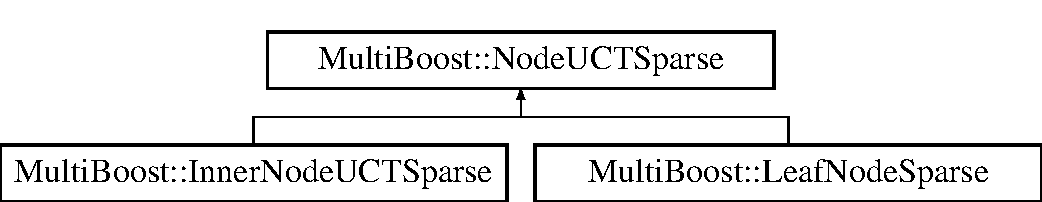
\includegraphics[height=2.000000cm]{classMultiBoost_1_1NodeUCTSparse}
\end{center}
\end{figure}
\subsection*{Public Member Functions}
\begin{DoxyCompactItemize}
\item 
\hypertarget{classMultiBoost_1_1NodeUCTSparse_a1c4ca3766d6175ddf11869c6e367be66}{virtual bool {\bfseries is\-Leaf} ()=0}\label{classMultiBoost_1_1NodeUCTSparse_a1c4ca3766d6175ddf11869c6e367be66}

\item 
\hypertarget{classMultiBoost_1_1NodeUCTSparse_ae0cd04afa5f85c126ac15606016241f4}{bool {\bfseries is\-Root} ()}\label{classMultiBoost_1_1NodeUCTSparse_ae0cd04afa5f85c126ac15606016241f4}

\item 
\hypertarget{classMultiBoost_1_1NodeUCTSparse_a4c23edb3d1b2b6daa794afab117342d2}{virtual int {\bfseries get\-Ni} ()}\label{classMultiBoost_1_1NodeUCTSparse_a4c23edb3d1b2b6daa794afab117342d2}

\item 
\hypertarget{classMultiBoost_1_1NodeUCTSparse_aa813626843e28a88a7596de6b8c2f02c}{virtual double {\bfseries get\-Xini} ()}\label{classMultiBoost_1_1NodeUCTSparse_aa813626843e28a88a7596de6b8c2f02c}

\item 
\hypertarget{classMultiBoost_1_1NodeUCTSparse_aa52c60fcdc6a4e94cc7af076948ba513}{virtual void {\bfseries inc\-Ni} ()}\label{classMultiBoost_1_1NodeUCTSparse_aa52c60fcdc6a4e94cc7af076948ba513}

\item 
\hypertarget{classMultiBoost_1_1NodeUCTSparse_ac5a2400bc3006db0059e5e6c65dd2aad}{virtual \hyperlink{classMultiBoost_1_1NodeUCTSparse}{Node\-U\-C\-T\-Sparse} $\ast$ {\bfseries get\-Parent} ()}\label{classMultiBoost_1_1NodeUCTSparse_ac5a2400bc3006db0059e5e6c65dd2aad}

\item 
\hypertarget{classMultiBoost_1_1NodeUCTSparse_a4ee398d1d1f7a4710a65d83b69c92c59}{virtual void {\bfseries add\-Value} (double val)}\label{classMultiBoost_1_1NodeUCTSparse_a4ee398d1d1f7a4710a65d83b69c92c59}

\item 
\hypertarget{classMultiBoost_1_1NodeUCTSparse_a4d12a61497753ed8f905fe1a6ede51fd}{virtual double {\bfseries get\-Upper\-Confidence\-Bound} ()}\label{classMultiBoost_1_1NodeUCTSparse_a4d12a61497753ed8f905fe1a6ede51fd}

\item 
\hypertarget{classMultiBoost_1_1NodeUCTSparse_a54dc4ac2dd9693cd3e5d3612dfeb2768}{virtual \hyperlink{classMultiBoost_1_1NodeUCTSparse}{Node\-U\-C\-T\-Sparse} $\ast$ {\bfseries getith\-Child} (int num)=0}\label{classMultiBoost_1_1NodeUCTSparse_a54dc4ac2dd9693cd3e5d3612dfeb2768}

\item 
\hypertarget{classMultiBoost_1_1NodeUCTSparse_aad6d27c2bcf2e173f60e342af77e9d34}{virtual void {\bfseries clear\-Inner\-Node\-Child} ()=0}\label{classMultiBoost_1_1NodeUCTSparse_aad6d27c2bcf2e173f60e342af77e9d34}

\item 
\hypertarget{classMultiBoost_1_1NodeUCTSparse_a224e3dffdfee2ceab08dfc257f40fe72}{virtual int {\bfseries get\-Num\-Of\-Child} ()=0}\label{classMultiBoost_1_1NodeUCTSparse_a224e3dffdfee2ceab08dfc257f40fe72}

\item 
\hypertarget{classMultiBoost_1_1NodeUCTSparse_a34ded869493de12e8d07b9e52c811ebc}{virtual int {\bfseries get\-Child\-Ind\-With\-Max\-Bi} ()=0}\label{classMultiBoost_1_1NodeUCTSparse_a34ded869493de12e8d07b9e52c811ebc}

\item 
\hypertarget{classMultiBoost_1_1NodeUCTSparse_a949058a4e4e112c9839da4f6035653ef}{virtual int {\bfseries get\-My\-Depth} ()}\label{classMultiBoost_1_1NodeUCTSparse_a949058a4e4e112c9839da4f6035653ef}

\item 
\hypertarget{classMultiBoost_1_1NodeUCTSparse_a171ce34b82f4f9c5bffac342c855cf43}{virtual void {\bfseries set\-My\-Depth} (int d)}\label{classMultiBoost_1_1NodeUCTSparse_a171ce34b82f4f9c5bffac342c855cf43}

\end{DoxyCompactItemize}
\subsection*{Static Public Member Functions}
\begin{DoxyCompactItemize}
\item 
\hypertarget{classMultiBoost_1_1NodeUCTSparse_a6e040f818807501ae8bc551e0197bd93}{static void {\bfseries set\-Depth} (int d)}\label{classMultiBoost_1_1NodeUCTSparse_a6e040f818807501ae8bc551e0197bd93}

\item 
\hypertarget{classMultiBoost_1_1NodeUCTSparse_a4d866c7cb583fe6d6090daeec9bed3cf}{static int {\bfseries get\-Depth} ()}\label{classMultiBoost_1_1NodeUCTSparse_a4d866c7cb583fe6d6090daeec9bed3cf}

\item 
\hypertarget{classMultiBoost_1_1NodeUCTSparse_a500e590f3688668e01f001481c6f77ed}{static void {\bfseries set\-Branch\-Order} (int bo)}\label{classMultiBoost_1_1NodeUCTSparse_a500e590f3688668e01f001481c6f77ed}

\end{DoxyCompactItemize}
\subsection*{Protected Attributes}
\begin{DoxyCompactItemize}
\item 
\hypertarget{classMultiBoost_1_1NodeUCTSparse_a196bc201d3bb99ee97c300fc2a5f7ba4}{\hyperlink{classMultiBoost_1_1NodeUCTSparse}{Node\-U\-C\-T\-Sparse} $\ast$ {\bfseries \-\_\-parent}}\label{classMultiBoost_1_1NodeUCTSparse_a196bc201d3bb99ee97c300fc2a5f7ba4}

\item 
\hypertarget{classMultiBoost_1_1NodeUCTSparse_a52aff0019a4d1d5b4175137ac1e5c79e}{int {\bfseries \-\_\-feature\-I\-D}}\label{classMultiBoost_1_1NodeUCTSparse_a52aff0019a4d1d5b4175137ac1e5c79e}

\item 
\hypertarget{classMultiBoost_1_1NodeUCTSparse_a3fd21c96d8ba30e4e9761b05f73c5209}{int {\bfseries \-\_\-ni}}\label{classMultiBoost_1_1NodeUCTSparse_a3fd21c96d8ba30e4e9761b05f73c5209}

\item 
\hypertarget{classMultiBoost_1_1NodeUCTSparse_ac1214966188530e2699af3f4c5175cd7}{double {\bfseries \-\_\-\-Xini}}\label{classMultiBoost_1_1NodeUCTSparse_ac1214966188530e2699af3f4c5175cd7}

\item 
\hypertarget{classMultiBoost_1_1NodeUCTSparse_aa069be2e0bbff09a798334f1d9b612a3}{int {\bfseries \-\_\-my\-Depth}}\label{classMultiBoost_1_1NodeUCTSparse_aa069be2e0bbff09a798334f1d9b612a3}

\end{DoxyCompactItemize}
\subsection*{Static Protected Attributes}
\begin{DoxyCompactItemize}
\item 
\hypertarget{classMultiBoost_1_1NodeUCTSparse_a4403071a5e5e157cad4c5082b9003dee}{static int {\bfseries \-\_\-depth} = 0}\label{classMultiBoost_1_1NodeUCTSparse_a4403071a5e5e157cad4c5082b9003dee}

\item 
\hypertarget{classMultiBoost_1_1NodeUCTSparse_ab910316c6b2bd4b4c9d7571c13307fdb}{static int {\bfseries \-\_\-branch\-Order} = 0}\label{classMultiBoost_1_1NodeUCTSparse_ab910316c6b2bd4b4c9d7571c13307fdb}

\end{DoxyCompactItemize}


\subsection{Detailed Description}


Definition at line 71 of file U\-C\-Tutils.\-h.



The documentation for this class was generated from the following files\-:\begin{DoxyCompactItemize}
\item 
C\-:/\-Users/fradav/\-Documents/\-Dev/\-C++/\-Multiboost/\-Sources/src/\-Utils/U\-C\-Tutils.\-h\item 
C\-:/\-Users/fradav/\-Documents/\-Dev/\-C++/\-Multiboost/\-Sources/src/\-Utils/U\-C\-Tutils.\-cpp\end{DoxyCompactItemize}

\hypertarget{classMultiBoost_1_1OneClassStumpAlgorithm}{\section{Multi\-Boost\-:\-:One\-Class\-Stump\-Algorithm$<$ T $>$ Class Template Reference}
\label{classMultiBoost_1_1OneClassStumpAlgorithm}\index{Multi\-Boost\-::\-One\-Class\-Stump\-Algorithm$<$ T $>$@{Multi\-Boost\-::\-One\-Class\-Stump\-Algorithm$<$ T $>$}}
}


{\ttfamily \#include $<$One\-Class\-Stump\-Algorithm.\-h$>$}

Inheritance diagram for Multi\-Boost\-:\-:One\-Class\-Stump\-Algorithm$<$ T $>$\-:\begin{figure}[H]
\begin{center}
\leavevmode
\includegraphics[height=2.000000cm]{classMultiBoost_1_1OneClassStumpAlgorithm}
\end{center}
\end{figure}
\subsection*{Public Types}
\begin{DoxyCompactItemize}
\item 
typedef vector$<$ pair$<$ int, T $>$\\*
 $>$\-::const\-\_\-iterator \hyperlink{classMultiBoost_1_1OneClassStumpAlgorithm_a5ad69d710488cdd1aa350baf36c13384}{vp\-Iterator}
\item 
typedef vector$<$ pair$<$ int, T $>$\\*
 $>$\-::const\-\_\-iterator \hyperlink{classMultiBoost_1_1OneClassStumpAlgorithm_a814d7366f9bcbcfd50a04ea0102ac6d9}{cvp\-Iterator}
\end{DoxyCompactItemize}
\subsection*{Public Member Functions}
\begin{DoxyCompactItemize}
\item 
\hypertarget{classMultiBoost_1_1OneClassStumpAlgorithm_ad7cbdbcc4a6576177ec18cf2d1e05a22}{{\bfseries One\-Class\-Stump\-Algorithm} (int num\-Classes)}\label{classMultiBoost_1_1OneClassStumpAlgorithm_ad7cbdbcc4a6576177ec18cf2d1e05a22}

\item 
\hypertarget{classMultiBoost_1_1OneClassStumpAlgorithm_a0c59e11de4a72bdf391a18d097bbb1af}{\hyperlink{Defaults_8h_a3a11cfe6a5d469d921716ca6291e934f}{Feature\-Real} {\bfseries find\-Single\-Threshold\-With\-Init} (const \hyperlink{classMultiBoost_1_1OneClassStumpAlgorithm_a5ad69d710488cdd1aa350baf36c13384}{vp\-Iterator} \&data\-Begin, const \hyperlink{classMultiBoost_1_1OneClassStumpAlgorithm_a5ad69d710488cdd1aa350baf36c13384}{vp\-Iterator} \&data\-End, \hyperlink{classMultiBoost_1_1InputData}{Input\-Data} $\ast$p\-Data, \hyperlink{Defaults_8h_a80184c4fd10ab70a1a17c5f97dcd1563}{Alpha\-Real} half\-Theta, vector$<$ \hyperlink{structMultiBoost_1_1sRates}{s\-Rates} $>$ $\ast$p\-Mu=N\-U\-L\-L, vector$<$ \hyperlink{Defaults_8h_a80184c4fd10ab70a1a17c5f97dcd1563}{Alpha\-Real} $>$ $\ast$p\-V=N\-U\-L\-L)}\label{classMultiBoost_1_1OneClassStumpAlgorithm_a0c59e11de4a72bdf391a18d097bbb1af}

\end{DoxyCompactItemize}
\subsection*{Additional Inherited Members}


\subsection{Detailed Description}
\subsubsection*{template$<$typename T$>$class Multi\-Boost\-::\-One\-Class\-Stump\-Algorithm$<$ T $>$}

Class specialized in solving decision stump-\/type algorithms. A decision stump is a decision tree with a single level. 

Definition at line 64 of file One\-Class\-Stump\-Algorithm.\-h.



\subsection{Member Typedef Documentation}
\hypertarget{classMultiBoost_1_1OneClassStumpAlgorithm_a814d7366f9bcbcfd50a04ea0102ac6d9}{\index{Multi\-Boost\-::\-One\-Class\-Stump\-Algorithm@{Multi\-Boost\-::\-One\-Class\-Stump\-Algorithm}!cvp\-Iterator@{cvp\-Iterator}}
\index{cvp\-Iterator@{cvp\-Iterator}!MultiBoost::OneClassStumpAlgorithm@{Multi\-Boost\-::\-One\-Class\-Stump\-Algorithm}}
\subsubsection[{cvp\-Iterator}]{\setlength{\rightskip}{0pt plus 5cm}template$<$typename T$>$ typedef vector$<$ pair$<$int, T$>$ $>$\-::const\-\_\-iterator {\bf Multi\-Boost\-::\-One\-Class\-Stump\-Algorithm}$<$ T $>$\-::{\bf cvp\-Iterator}}}\label{classMultiBoost_1_1OneClassStumpAlgorithm_a814d7366f9bcbcfd50a04ea0102ac6d9}
Const iterator on Pair. The pair refers to $<$index, value$>$. 

Definition at line 75 of file One\-Class\-Stump\-Algorithm.\-h.

\hypertarget{classMultiBoost_1_1OneClassStumpAlgorithm_a5ad69d710488cdd1aa350baf36c13384}{\index{Multi\-Boost\-::\-One\-Class\-Stump\-Algorithm@{Multi\-Boost\-::\-One\-Class\-Stump\-Algorithm}!vp\-Iterator@{vp\-Iterator}}
\index{vp\-Iterator@{vp\-Iterator}!MultiBoost::OneClassStumpAlgorithm@{Multi\-Boost\-::\-One\-Class\-Stump\-Algorithm}}
\subsubsection[{vp\-Iterator}]{\setlength{\rightskip}{0pt plus 5cm}template$<$typename T$>$ typedef vector$<$ pair$<$int, T$>$ $>$\-::const\-\_\-iterator {\bf Multi\-Boost\-::\-One\-Class\-Stump\-Algorithm}$<$ T $>$\-::{\bf vp\-Iterator}}}\label{classMultiBoost_1_1OneClassStumpAlgorithm_a5ad69d710488cdd1aa350baf36c13384}
Iterator on Pair. The pair refers to $<$index, value$>$. 

Definition at line 71 of file One\-Class\-Stump\-Algorithm.\-h.



The documentation for this class was generated from the following file\-:\begin{DoxyCompactItemize}
\item 
C\-:/\-Users/fradav/\-Documents/\-Dev/\-C++/\-Multiboost/\-Sources/src/\-Algorithms/\hyperlink{OneClassStumpAlgorithm_8h}{One\-Class\-Stump\-Algorithm.\-h}\end{DoxyCompactItemize}

\hypertarget{classMultiBoost_1_1OneClassStumpLearner}{
\section{MultiBoost::OneClassStumpLearner Class Reference}
\label{classMultiBoost_1_1OneClassStumpLearner}\index{MultiBoost::OneClassStumpLearner@{MultiBoost::OneClassStumpLearner}}
}


{\ttfamily \#include $<$OneClassStumpLearner.h$>$}

Inheritance diagram for MultiBoost::OneClassStumpLearner:\begin{figure}[H]
\begin{center}
\leavevmode
\includegraphics[height=3.211009cm]{classMultiBoost_1_1OneClassStumpLearner}
\end{center}
\end{figure}
\subsection*{Public Member Functions}
\begin{DoxyCompactItemize}
\item 
virtual \hyperlink{classMultiBoost_1_1OneClassStumpLearner_a1950c8ee328113ce758232175e30e197}{$\sim$OneClassStumpLearner} ()
\item 
virtual \hyperlink{classMultiBoost_1_1BaseLearner}{BaseLearner} $\ast$ \hyperlink{classMultiBoost_1_1OneClassStumpLearner_ac00d7c627e63188969086c4731d1e108}{subCreate} ()
\item 
virtual \hyperlink{Defaults_8h_a80184c4fd10ab70a1a17c5f97dcd1563}{AlphaReal} \hyperlink{classMultiBoost_1_1OneClassStumpLearner_ab2ef660fcf6f95e176901a82c1904fe9}{run} ()
\item 
virtual \hyperlink{Defaults_8h_a80184c4fd10ab70a1a17c5f97dcd1563}{AlphaReal} \hyperlink{classMultiBoost_1_1OneClassStumpLearner_a01ca9c278f874d051382080b1eff990f}{run} (int colIdx)
\item 
virtual \hyperlink{Defaults_8h_a80184c4fd10ab70a1a17c5f97dcd1563}{AlphaReal} \hyperlink{classMultiBoost_1_1OneClassStumpLearner_a0c4f50119ccb0eda9a3857fddd00fbae}{run} (vector$<$ int $>$ \&colIndexes)
\end{DoxyCompactItemize}


\subsection{Detailed Description}
A {\bfseries single} threshold decision stump learner. There is ONE and ONE ONLY threshold here. 

Definition at line 63 of file OneClassStumpLearner.h.



\subsection{Constructor \& Destructor Documentation}
\hypertarget{classMultiBoost_1_1OneClassStumpLearner_a1950c8ee328113ce758232175e30e197}{
\index{MultiBoost::OneClassStumpLearner@{MultiBoost::OneClassStumpLearner}!$\sim$OneClassStumpLearner@{$\sim$OneClassStumpLearner}}
\index{$\sim$OneClassStumpLearner@{$\sim$OneClassStumpLearner}!MultiBoost::OneClassStumpLearner@{MultiBoost::OneClassStumpLearner}}
\subsubsection[{$\sim$OneClassStumpLearner}]{\setlength{\rightskip}{0pt plus 5cm}virtual MultiBoost::OneClassStumpLearner::$\sim$OneClassStumpLearner (
\begin{DoxyParamCaption}
{}
\end{DoxyParamCaption}
)\hspace{0.3cm}{\ttfamily  \mbox{[}inline, virtual\mbox{]}}}}
\label{classMultiBoost_1_1OneClassStumpLearner_a1950c8ee328113ce758232175e30e197}
The destructor. Must be declared (virtual) for the proper destruction of the object. 

Definition at line 73 of file OneClassStumpLearner.h.



\subsection{Member Function Documentation}
\hypertarget{classMultiBoost_1_1OneClassStumpLearner_ab2ef660fcf6f95e176901a82c1904fe9}{
\index{MultiBoost::OneClassStumpLearner@{MultiBoost::OneClassStumpLearner}!run@{run}}
\index{run@{run}!MultiBoost::OneClassStumpLearner@{MultiBoost::OneClassStumpLearner}}
\subsubsection[{run}]{\setlength{\rightskip}{0pt plus 5cm}{\bf AlphaReal} MultiBoost::OneClassStumpLearner::run (
\begin{DoxyParamCaption}
{}
\end{DoxyParamCaption}
)\hspace{0.3cm}{\ttfamily  \mbox{[}virtual\mbox{]}}}}
\label{classMultiBoost_1_1OneClassStumpLearner_ab2ef660fcf6f95e176901a82c1904fe9}
Run the learner to build the classifier on the given data. 
\begin{DoxyParams}{Parameters}
{\em pData} & The pointer to the data. \\
\hline
\end{DoxyParams}
\begin{DoxySeeAlso}{See also}
\hyperlink{classMultiBoost_1_1BaseLearner_a525e8f10782055b5c9762318e6e9768e}{BaseLearner::run} 
\end{DoxySeeAlso}
\begin{DoxyDate}{Date}
11/11/2005 
\end{DoxyDate}


Reimplemented from \hyperlink{classMultiBoost_1_1SingleStumpLearner_a9cd7bfe1a0905857993eec0dd462a879}{MultiBoost::SingleStumpLearner}.



Definition at line 51 of file OneClassStumpLearner.cpp.

\hypertarget{classMultiBoost_1_1OneClassStumpLearner_a0c4f50119ccb0eda9a3857fddd00fbae}{
\index{MultiBoost::OneClassStumpLearner@{MultiBoost::OneClassStumpLearner}!run@{run}}
\index{run@{run}!MultiBoost::OneClassStumpLearner@{MultiBoost::OneClassStumpLearner}}
\subsubsection[{run}]{\setlength{\rightskip}{0pt plus 5cm}{\bf AlphaReal} MultiBoost::OneClassStumpLearner::run (
\begin{DoxyParamCaption}
\item[{vector$<$ int $>$ \&}]{colIndices}
\end{DoxyParamCaption}
)\hspace{0.3cm}{\ttfamily  \mbox{[}virtual\mbox{]}}}}
\label{classMultiBoost_1_1OneClassStumpLearner_a0c4f50119ccb0eda9a3857fddd00fbae}
Run the learner to build the classifier using only a subset of features from the given data. 
\begin{DoxyParams}{Parameters}
{\em pData} & The pointer to the data. \\
\hline
\end{DoxyParams}
\begin{DoxyWarning}{Warning}
This function {\bfseries must} update \_\-alpha too! You can use the helper functions (the getAlpha with parameters) to update it.  colIndices The indices of the features can be only used. 
\end{DoxyWarning}
\begin{DoxyReturn}{Returns}
The energy of the weak classifier (that we want to minimize) 
\end{DoxyReturn}
\begin{DoxySeeAlso}{See also}
getAlpha(float) 

getAlpha(float, float) 

getAlpha(float, float, float, float) 
\end{DoxySeeAlso}


Reimplemented from \hyperlink{classMultiBoost_1_1FeaturewiseLearner_a2813c451210fc9d4fb4cf96216bcc813}{MultiBoost::FeaturewiseLearner}.



Definition at line 203 of file OneClassStumpLearner.cpp.

\hypertarget{classMultiBoost_1_1OneClassStumpLearner_a01ca9c278f874d051382080b1eff990f}{
\index{MultiBoost::OneClassStumpLearner@{MultiBoost::OneClassStumpLearner}!run@{run}}
\index{run@{run}!MultiBoost::OneClassStumpLearner@{MultiBoost::OneClassStumpLearner}}
\subsubsection[{run}]{\setlength{\rightskip}{0pt plus 5cm}{\bf AlphaReal} MultiBoost::OneClassStumpLearner::run (
\begin{DoxyParamCaption}
\item[{int}]{colIdx}
\end{DoxyParamCaption}
)\hspace{0.3cm}{\ttfamily  \mbox{[}virtual\mbox{]}}}}
\label{classMultiBoost_1_1OneClassStumpLearner_a01ca9c278f874d051382080b1eff990f}
Run the learner to build the classifier using only one single feature from the given data. 
\begin{DoxyParams}{Parameters}
{\em pData} & The pointer to the data. \\
\hline
\end{DoxyParams}
\begin{DoxyWarning}{Warning}
This function {\bfseries must} update \_\-alpha too! You can use the helper functions (the getAlpha with parameters) to update it.  colIdx The index of the feature can be only used. 
\end{DoxyWarning}
\begin{DoxyReturn}{Returns}
The energy of the weak classifier (that we want to minimize) 
\end{DoxyReturn}
\begin{DoxySeeAlso}{See also}
getAlpha(float) 

getAlpha(float, float) 

getAlpha(float, float, float, float) 
\end{DoxySeeAlso}


Implements \hyperlink{classMultiBoost_1_1FeaturewiseLearner_a534117f1fd7727e54fbef8594e187d04}{MultiBoost::FeaturewiseLearner}.



Definition at line 147 of file OneClassStumpLearner.cpp.

\hypertarget{classMultiBoost_1_1OneClassStumpLearner_ac00d7c627e63188969086c4731d1e108}{
\index{MultiBoost::OneClassStumpLearner@{MultiBoost::OneClassStumpLearner}!subCreate@{subCreate}}
\index{subCreate@{subCreate}!MultiBoost::OneClassStumpLearner@{MultiBoost::OneClassStumpLearner}}
\subsubsection[{subCreate}]{\setlength{\rightskip}{0pt plus 5cm}virtual {\bf BaseLearner}$\ast$ MultiBoost::OneClassStumpLearner::subCreate (
\begin{DoxyParamCaption}
{}
\end{DoxyParamCaption}
)\hspace{0.3cm}{\ttfamily  \mbox{[}inline, virtual\mbox{]}}}}
\label{classMultiBoost_1_1OneClassStumpLearner_ac00d7c627e63188969086c4731d1e108}
Returns itself as object. \begin{DoxyRemark}{Remarks}
It uses the trick described in \href{http://www.parashift.com/c++-faq-lite/serialization.html#faq-36.8}{\tt http://www.parashift.com/c++-\/faq-\/lite/serialization.html\#faq-\/36.8} for the auto-\/registering classes. 
\end{DoxyRemark}
\begin{DoxyDate}{Date}
14/11/2005 
\end{DoxyDate}


Reimplemented from \hyperlink{classMultiBoost_1_1SingleStumpLearner_ac78a95b491c3cef2362c6459f2465288}{MultiBoost::SingleStumpLearner}.



Definition at line 81 of file OneClassStumpLearner.h.



The documentation for this class was generated from the following files:\begin{DoxyCompactItemize}
\item 
/cygdrive/c/Users/fradav/Documents/Dev/Multiboost/Sources/src/WeakLearners/\hyperlink{OneClassStumpLearner_8h}{OneClassStumpLearner.h}\item 
/cygdrive/c/Users/fradav/Documents/Dev/Multiboost/Sources/src/WeakLearners/OneClassStumpLearner.cpp\end{DoxyCompactItemize}

\hypertarget{classMultiBoost_1_1OutputInfo}{\section{Multi\-Boost\-:\-:Output\-Info Class Reference}
\label{classMultiBoost_1_1OutputInfo}\index{Multi\-Boost\-::\-Output\-Info@{Multi\-Boost\-::\-Output\-Info}}
}


{\ttfamily \#include $<$Output\-Info.\-h$>$}

\subsection*{Public Member Functions}
\begin{DoxyCompactItemize}
\item 
\hyperlink{classMultiBoost_1_1OutputInfo_a5f5b3b2096d1c332701272d2480411e1}{Output\-Info} (const \hyperlink{classnor__utils_1_1Args}{nor\-\_\-utils\-::\-Args} \&args, bool custom\-Update=false, const string \&cl\-Arg=\char`\"{}outputinfo\char`\"{})
\item 
void \hyperlink{classMultiBoost_1_1OutputInfo_a247a59efd5c6270488009f15c36c84aa}{set\-Output\-List} (const string \&list, const \hyperlink{classnor__utils_1_1Args}{nor\-\_\-utils\-::\-Args} $\ast$args=N\-U\-L\-L)
\item 
void \hyperlink{classMultiBoost_1_1OutputInfo_ac9210d45cb3c2ed39365f55bd63d1c76}{output\-Iteration} (int t)
\item 
\hypertarget{classMultiBoost_1_1OutputInfo_a165b4d7f473ab024df0d29fd5b43c730}{void {\bfseries initialize} (\hyperlink{classMultiBoost_1_1InputData}{Input\-Data} $\ast$p\-Data)}\label{classMultiBoost_1_1OutputInfo_a165b4d7f473ab024df0d29fd5b43c730}

\item 
void \hyperlink{classMultiBoost_1_1OutputInfo_a5a12b37b0fe9129ea59616829961dadf}{output\-Current\-Time} (void)
\item 
void \hyperlink{classMultiBoost_1_1OutputInfo_a563f8258a59d62a1a432d9616cb09c22}{output\-Header} (const \hyperlink{classMultiBoost_1_1NameMap}{Name\-Map} \&namemap, bool output\-Iterations=true, bool output\-Time=true, bool endline=true)
\item 
\hyperlink{Defaults_8h_a80184c4fd10ab70a1a17c5f97dcd1563}{Alpha\-Real} \hyperlink{classMultiBoost_1_1OutputInfo_a931359742e0d526a9055b47da82c438a}{get\-Sum\-Of\-Alphas} (\hyperlink{classMultiBoost_1_1InputData}{Input\-Data} $\ast$p\-Data)
\item 
void \hyperlink{classMultiBoost_1_1OutputInfo_a3e609b64c68fdf8392a969e2f6890941}{output\-Custom} (\hyperlink{classMultiBoost_1_1InputData}{Input\-Data} $\ast$p\-Data, \hyperlink{classMultiBoost_1_1BaseLearner}{Base\-Learner} $\ast$p\-Weak\-Hypothesis=0)
\item 
void \hyperlink{classMultiBoost_1_1OutputInfo_a4d9d20e123fdc12c5d4999d6ae6e444a}{end\-Line} ()
\item 
\hypertarget{classMultiBoost_1_1OutputInfo_aead6cdf710ccd7580700eb415d9475c5}{void {\bfseries header\-End\-Line} ()}\label{classMultiBoost_1_1OutputInfo_aead6cdf710ccd7580700eb415d9475c5}

\item 
void \hyperlink{classMultiBoost_1_1OutputInfo_a215f08683e3d7bdf75c338f564613d7f}{separator} ()
\item 
\hypertarget{classMultiBoost_1_1OutputInfo_afb3deba5970afb8d5ddf44f93abce2ec}{void {\bfseries output\-User\-Data} (float data)}\label{classMultiBoost_1_1OutputInfo_afb3deba5970afb8d5ddf44f93abce2ec}

\item 
\hypertarget{classMultiBoost_1_1OutputInfo_ae10ed27b4a35d03f15f9747eff1f6794}{void {\bfseries output\-User\-Header} (const string \&h)}\label{classMultiBoost_1_1OutputInfo_ae10ed27b4a35d03f15f9747eff1f6794}

\item 
\hypertarget{classMultiBoost_1_1OutputInfo_a9403bd66833a538689d1e0cd6152879e}{table \& {\bfseries get\-Table} (\hyperlink{classMultiBoost_1_1InputData}{Input\-Data} $\ast$p\-Data)}\label{classMultiBoost_1_1OutputInfo_a9403bd66833a538689d1e0cd6152879e}

\item 
\hypertarget{classMultiBoost_1_1OutputInfo_ab3d1c1abc253f07e501b53765bd4292c}{void {\bfseries set\-Table} (\hyperlink{classMultiBoost_1_1InputData}{Input\-Data} $\ast$p\-Data, table \&tmp\-Table)}\label{classMultiBoost_1_1OutputInfo_ab3d1c1abc253f07e501b53765bd4292c}

\item 
\hypertarget{classMultiBoost_1_1OutputInfo_a4ad5ceba66d6212c548ea6d5cd072f50}{table \& {\bfseries get\-Margins} (\hyperlink{classMultiBoost_1_1InputData}{Input\-Data} $\ast$p\-Data)}\label{classMultiBoost_1_1OutputInfo_a4ad5ceba66d6212c548ea6d5cd072f50}

\item 
\hypertarget{classMultiBoost_1_1OutputInfo_af3dca3903e4aae0d0787013568f60ebf}{void {\bfseries update\-Tables} (\hyperlink{classMultiBoost_1_1InputData}{Input\-Data} $\ast$p\-Data, \hyperlink{classMultiBoost_1_1BaseLearner}{Base\-Learner} $\ast$p\-Weak\-Hypothesis)}\label{classMultiBoost_1_1OutputInfo_af3dca3903e4aae0d0787013568f60ebf}

\item 
\hyperlink{classMultiBoost_1_1BaseOutputInfoType}{Base\-Output\-Info\-Type} $\ast$ \hyperlink{classMultiBoost_1_1OutputInfo_a3ca4fbc83b4acb298bb0ac887c22af4f}{get\-Output\-Info\-Object} (const string \&type)
\item 
\hyperlink{Defaults_8h_a80184c4fd10ab70a1a17c5f97dcd1563}{Alpha\-Real} \hyperlink{classMultiBoost_1_1OutputInfo_adbb38b8ab53a523227c756a7fab94866}{get\-Output\-History} (\hyperlink{classMultiBoost_1_1InputData}{Input\-Data} $\ast$p\-Data, const string \&output\-Name, int iteration=-\/1)
\item 
bool \hyperlink{classMultiBoost_1_1OutputInfo_a2b37cd3f75fae8de97ef05401a70798e}{output\-Is\-Activated} (const string \&output\-Name)
\item 
\hypertarget{classMultiBoost_1_1OutputInfo_a25944722d385ef55a8b4aa31e547682f}{void {\bfseries set\-Starting\-Iteration} (unsigned int i)}\label{classMultiBoost_1_1OutputInfo_a25944722d385ef55a8b4aa31e547682f}

\end{DoxyCompactItemize}
\subsection*{Protected Member Functions}
\begin{DoxyCompactItemize}
\item 
void \hyperlink{classMultiBoost_1_1OutputInfo_a0c6dfc8babe3815d10888d2ec7c6ccc9}{get\-Output\-List\-From\-String} (const string \&list, const \hyperlink{classnor__utils_1_1Args}{nor\-\_\-utils\-::\-Args} $\ast$args=N\-U\-L\-L)
\end{DoxyCompactItemize}
\subsection*{Protected Attributes}
\begin{DoxyCompactItemize}
\item 
\hypertarget{classMultiBoost_1_1OutputInfo_a9218ec74c3b278be4ad81d90a93d5535}{fstream \hyperlink{classMultiBoost_1_1OutputInfo_a9218ec74c3b278be4ad81d90a93d5535}{\-\_\-out\-Stream}}\label{classMultiBoost_1_1OutputInfo_a9218ec74c3b278be4ad81d90a93d5535}

\begin{DoxyCompactList}\small\item\em The output stream. \end{DoxyCompactList}\item 
\hypertarget{classMultiBoost_1_1OutputInfo_a412abadc6b0171bf233890c00965e62a}{time\-\_\-t {\bfseries \-\_\-begining\-Time}}\label{classMultiBoost_1_1OutputInfo_a412abadc6b0171bf233890c00965e62a}

\item 
\hypertarget{classMultiBoost_1_1OutputInfo_a241d192ace61b9ae826e0e076a625980}{time\-\_\-t {\bfseries \-\_\-time\-Bias}}\label{classMultiBoost_1_1OutputInfo_a241d192ace61b9ae826e0e076a625980}

\item 
map$<$ \hyperlink{classMultiBoost_1_1InputData}{Input\-Data} $\ast$, table $>$ \hyperlink{classMultiBoost_1_1OutputInfo_a0d95c1f68bad97c49e0333bdde066940}{\-\_\-g\-Table\-Map}
\item 
map$<$ \hyperlink{classMultiBoost_1_1InputData}{Input\-Data} $\ast$, table $>$ \hyperlink{classMultiBoost_1_1OutputInfo_a350f1c9355d0602ec20c99ed70491e85}{\-\_\-margins}
\item 
map$<$ \hyperlink{classMultiBoost_1_1InputData}{Input\-Data} $\ast$, \hyperlink{Defaults_8h_a80184c4fd10ab70a1a17c5f97dcd1563}{Alpha\-Real} $>$ \hyperlink{classMultiBoost_1_1OutputInfo_ad887f8e1b0f0be528082f28e3514879b}{\-\_\-alpha\-Sums}
\item 
\hypertarget{classMultiBoost_1_1OutputInfo_ab0d7902cb985b047a13671c1cc0991a1}{map$<$ string, \hyperlink{classMultiBoost_1_1BaseOutputInfoType}{Base\-Output\-Info\-Type} $\ast$ $>$ {\bfseries \-\_\-output\-List}}\label{classMultiBoost_1_1OutputInfo_ab0d7902cb985b047a13671c1cc0991a1}

\item 
\hypertarget{classMultiBoost_1_1OutputInfo_a52ee1e8382ca696534809caba70b7de3}{bool {\bfseries \-\_\-custom\-Tables\-Update}}\label{classMultiBoost_1_1OutputInfo_a52ee1e8382ca696534809caba70b7de3}

\item 
fstream \hyperlink{classMultiBoost_1_1OutputInfo_a18631871093bb6fb65a4ebb0e50909a4}{\-\_\-header\-Out\-Stream}
\item 
\hypertarget{classMultiBoost_1_1OutputInfo_a7bfc2b437c1772c4e09966e875d3d391}{unsigned int {\bfseries \-\_\-history\-Starting\-Iteration}}\label{classMultiBoost_1_1OutputInfo_a7bfc2b437c1772c4e09966e875d3d391}

\end{DoxyCompactItemize}


\subsection{Detailed Description}
Format and output step-\/by-\/step information. With this class it is possible to output and update the error rates, margins and the edge. These function must be called at each iteration with the newly found weak hypothesis, but {\bfseries before} the update of the weights. \begin{DoxyWarning}{Warning}
Don't forget to begin the list of information printed with \hyperlink{classMultiBoost_1_1OutputInfo_ac9210d45cb3c2ed39365f55bd63d1c76}{output\-Iteration()}, and close it with a call to \hyperlink{classMultiBoost_1_1OutputInfo_a4d9d20e123fdc12c5d4999d6ae6e444a}{end\-Line()}! 
\end{DoxyWarning}
\begin{DoxyDate}{Date}
16/11/2005 
\end{DoxyDate}


Definition at line 92 of file Output\-Info.\-h.



\subsection{Constructor \& Destructor Documentation}
\hypertarget{classMultiBoost_1_1OutputInfo_a5f5b3b2096d1c332701272d2480411e1}{\index{Multi\-Boost\-::\-Output\-Info@{Multi\-Boost\-::\-Output\-Info}!Output\-Info@{Output\-Info}}
\index{Output\-Info@{Output\-Info}!MultiBoost::OutputInfo@{Multi\-Boost\-::\-Output\-Info}}
\subsubsection[{Output\-Info}]{\setlength{\rightskip}{0pt plus 5cm}Multi\-Boost\-::\-Output\-Info\-::\-Output\-Info (
\begin{DoxyParamCaption}
\item[{const {\bf nor\-\_\-utils\-::\-Args} \&}]{args, }
\item[{bool}]{custom\-Update = {\ttfamily false}, }
\item[{const string \&}]{cl\-Arg = {\ttfamily \char`\"{}outputinfo\char`\"{}}}
\end{DoxyParamCaption}
)\hspace{0.3cm}{\ttfamily [explicit]}}}\label{classMultiBoost_1_1OutputInfo_a5f5b3b2096d1c332701272d2480411e1}
The constructor. Create the object and open the output file. 
\begin{DoxyParams}{Parameters}
{\em args} & The arguments passed through command line \\
\hline
{\em cl\-Arg} & The command line argument that gives the output file name \\
\hline
\end{DoxyParams}
\begin{DoxyDate}{Date}
17/06/2011 
\end{DoxyDate}


Definition at line 48 of file Output\-Info.\-cpp.



\subsection{Member Function Documentation}
\hypertarget{classMultiBoost_1_1OutputInfo_a4d9d20e123fdc12c5d4999d6ae6e444a}{\index{Multi\-Boost\-::\-Output\-Info@{Multi\-Boost\-::\-Output\-Info}!end\-Line@{end\-Line}}
\index{end\-Line@{end\-Line}!MultiBoost::OutputInfo@{Multi\-Boost\-::\-Output\-Info}}
\subsubsection[{end\-Line}]{\setlength{\rightskip}{0pt plus 5cm}void Multi\-Boost\-::\-Output\-Info\-::end\-Line (
\begin{DoxyParamCaption}
{}
\end{DoxyParamCaption}
)\hspace{0.3cm}{\ttfamily [inline]}}}\label{classMultiBoost_1_1OutputInfo_a4d9d20e123fdc12c5d4999d6ae6e444a}
End of line in the file stream. Call it when all the needed information has been outputted. \begin{DoxyDate}{Date}
16/11/2005 
\end{DoxyDate}


Definition at line 163 of file Output\-Info.\-h.

\hypertarget{classMultiBoost_1_1OutputInfo_adbb38b8ab53a523227c756a7fab94866}{\index{Multi\-Boost\-::\-Output\-Info@{Multi\-Boost\-::\-Output\-Info}!get\-Output\-History@{get\-Output\-History}}
\index{get\-Output\-History@{get\-Output\-History}!MultiBoost::OutputInfo@{Multi\-Boost\-::\-Output\-Info}}
\subsubsection[{get\-Output\-History}]{\setlength{\rightskip}{0pt plus 5cm}{\bf Alpha\-Real} Multi\-Boost\-::\-Output\-Info\-::get\-Output\-History (
\begin{DoxyParamCaption}
\item[{{\bf Input\-Data} $\ast$}]{p\-Data, }
\item[{const string \&}]{output\-Name, }
\item[{int}]{iteration = {\ttfamily -\/1}}
\end{DoxyParamCaption}
)}}\label{classMultiBoost_1_1OutputInfo_adbb38b8ab53a523227c756a7fab94866}
Return the specific metric output for a given dataset and a given iteration. If the iteration is -\/1, it returns the last value. 
\begin{DoxyParams}{Parameters}
{\em p\-Data} & The dataset on which the metric was computed. \\
\hline
{\em output\-Name} & The three caracters code of the output (the same as for --outputinfo argument). \\
\hline
{\em iteration} & The iteration at which the metric was computed. \\
\hline
\end{DoxyParams}
\begin{DoxyDate}{Date}
05/04/2013 
\end{DoxyDate}


Definition at line 315 of file Output\-Info.\-cpp.

\hypertarget{classMultiBoost_1_1OutputInfo_a3ca4fbc83b4acb298bb0ac887c22af4f}{\index{Multi\-Boost\-::\-Output\-Info@{Multi\-Boost\-::\-Output\-Info}!get\-Output\-Info\-Object@{get\-Output\-Info\-Object}}
\index{get\-Output\-Info\-Object@{get\-Output\-Info\-Object}!MultiBoost::OutputInfo@{Multi\-Boost\-::\-Output\-Info}}
\subsubsection[{get\-Output\-Info\-Object}]{\setlength{\rightskip}{0pt plus 5cm}{\bf Base\-Output\-Info\-Type} $\ast$ Multi\-Boost\-::\-Output\-Info\-::get\-Output\-Info\-Object (
\begin{DoxyParamCaption}
\item[{const string \&}]{type}
\end{DoxyParamCaption}
)}}\label{classMultiBoost_1_1OutputInfo_a3ca4fbc83b4acb298bb0ac887c22af4f}
Calls the update\-Specific\-Info method for each Output\-Info\-Type subclass. The subclasses that implement this method must check whether the update is targetted to them or not through the prefix of the param type. 
\begin{DoxyParams}{Parameters}
{\em type} & The name of the info to be updated, it is highly recommanded to prefix this name by an abreviation of the class name. \\
\hline
{\em value} & The value to be added/updated \\
\hline
\end{DoxyParams}
\begin{DoxyDate}{Date}
05/07/2011 
\end{DoxyDate}


Definition at line 306 of file Output\-Info.\-cpp.

\hypertarget{classMultiBoost_1_1OutputInfo_a0c6dfc8babe3815d10888d2ec7c6ccc9}{\index{Multi\-Boost\-::\-Output\-Info@{Multi\-Boost\-::\-Output\-Info}!get\-Output\-List\-From\-String@{get\-Output\-List\-From\-String}}
\index{get\-Output\-List\-From\-String@{get\-Output\-List\-From\-String}!MultiBoost::OutputInfo@{Multi\-Boost\-::\-Output\-Info}}
\subsubsection[{get\-Output\-List\-From\-String}]{\setlength{\rightskip}{0pt plus 5cm}void Multi\-Boost\-::\-Output\-Info\-::get\-Output\-List\-From\-String (
\begin{DoxyParamCaption}
\item[{const string \&}]{list, }
\item[{const {\bf nor\-\_\-utils\-::\-Args} $\ast$}]{args = {\ttfamily NULL}}
\end{DoxyParamCaption}
)\hspace{0.3cm}{\ttfamily [protected]}}}\label{classMultiBoost_1_1OutputInfo_a0c6dfc8babe3815d10888d2ec7c6ccc9}
Creates the Output\-Info\-Type instances from a string \begin{DoxyDate}{Date}
04/07/2011 
\end{DoxyDate}


Definition at line 185 of file Output\-Info.\-cpp.

\hypertarget{classMultiBoost_1_1OutputInfo_a931359742e0d526a9055b47da82c438a}{\index{Multi\-Boost\-::\-Output\-Info@{Multi\-Boost\-::\-Output\-Info}!get\-Sum\-Of\-Alphas@{get\-Sum\-Of\-Alphas}}
\index{get\-Sum\-Of\-Alphas@{get\-Sum\-Of\-Alphas}!MultiBoost::OutputInfo@{Multi\-Boost\-::\-Output\-Info}}
\subsubsection[{get\-Sum\-Of\-Alphas}]{\setlength{\rightskip}{0pt plus 5cm}{\bf Alpha\-Real} Multi\-Boost\-::\-Output\-Info\-::get\-Sum\-Of\-Alphas (
\begin{DoxyParamCaption}
\item[{{\bf Input\-Data} $\ast$}]{p\-Data}
\end{DoxyParamCaption}
)\hspace{0.3cm}{\ttfamily [inline]}}}\label{classMultiBoost_1_1OutputInfo_a931359742e0d526a9055b47da82c438a}
Just return the sum of alphas 
\begin{DoxyParams}{Parameters}
{\em p\-Data} & pointer of the input data \\
\hline
\end{DoxyParams}
\begin{DoxyDate}{Date}
04/04/2012 
\end{DoxyDate}


Definition at line 142 of file Output\-Info.\-h.

\hypertarget{classMultiBoost_1_1OutputInfo_a5a12b37b0fe9129ea59616829961dadf}{\index{Multi\-Boost\-::\-Output\-Info@{Multi\-Boost\-::\-Output\-Info}!output\-Current\-Time@{output\-Current\-Time}}
\index{output\-Current\-Time@{output\-Current\-Time}!MultiBoost::OutputInfo@{Multi\-Boost\-::\-Output\-Info}}
\subsubsection[{output\-Current\-Time}]{\setlength{\rightskip}{0pt plus 5cm}void Multi\-Boost\-::\-Output\-Info\-::output\-Current\-Time (
\begin{DoxyParamCaption}
\item[{void}]{}
\end{DoxyParamCaption}
)}}\label{classMultiBoost_1_1OutputInfo_a5a12b37b0fe9129ea59616829961dadf}
Just output the current time. 
\begin{DoxyParams}{Parameters}
{\em \textbackslash{}date} & 14/11/2005 \\
\hline
\end{DoxyParams}


Definition at line 335 of file Output\-Info.\-cpp.

\hypertarget{classMultiBoost_1_1OutputInfo_a3e609b64c68fdf8392a969e2f6890941}{\index{Multi\-Boost\-::\-Output\-Info@{Multi\-Boost\-::\-Output\-Info}!output\-Custom@{output\-Custom}}
\index{output\-Custom@{output\-Custom}!MultiBoost::OutputInfo@{Multi\-Boost\-::\-Output\-Info}}
\subsubsection[{output\-Custom}]{\setlength{\rightskip}{0pt plus 5cm}void Multi\-Boost\-::\-Output\-Info\-::output\-Custom (
\begin{DoxyParamCaption}
\item[{{\bf Input\-Data} $\ast$}]{p\-Data, }
\item[{{\bf Base\-Learner} $\ast$}]{p\-Weak\-Hypothesis = {\ttfamily 0}}
\end{DoxyParamCaption}
)}}\label{classMultiBoost_1_1OutputInfo_a3e609b64c68fdf8392a969e2f6890941}
Output the information the user wants This \char`\"{}wish-\/list\char`\"{} is specified either through the command line or directly through the constructor 
\begin{DoxyParams}{Parameters}
{\em p\-Data} & The input data. \\
\hline
{\em p\-Weak\-Hypothesis} & The current weak hypothesis. \\
\hline
\end{DoxyParams}
\begin{DoxyDate}{Date}
17/06/2011 
\end{DoxyDate}


Definition at line 241 of file Output\-Info.\-cpp.

\hypertarget{classMultiBoost_1_1OutputInfo_a563f8258a59d62a1a432d9616cb09c22}{\index{Multi\-Boost\-::\-Output\-Info@{Multi\-Boost\-::\-Output\-Info}!output\-Header@{output\-Header}}
\index{output\-Header@{output\-Header}!MultiBoost::OutputInfo@{Multi\-Boost\-::\-Output\-Info}}
\subsubsection[{output\-Header}]{\setlength{\rightskip}{0pt plus 5cm}void Multi\-Boost\-::\-Output\-Info\-::output\-Header (
\begin{DoxyParamCaption}
\item[{const {\bf Name\-Map} \&}]{namemap, }
\item[{bool}]{output\-Iterations = {\ttfamily true}, }
\item[{bool}]{output\-Time = {\ttfamily true}, }
\item[{bool}]{endline = {\ttfamily true}}
\end{DoxyParamCaption}
)}}\label{classMultiBoost_1_1OutputInfo_a563f8258a59d62a1a432d9616cb09c22}
Output the column names Note that this method must be called after the initialization of all the datasets 
\begin{DoxyParams}{Parameters}
{\em namemap} & The structure that holds the class information \\
\hline
\end{DoxyParams}
\begin{DoxyDate}{Date}
04/08/2006 
\end{DoxyDate}


Definition at line 206 of file Output\-Info.\-cpp.

\hypertarget{classMultiBoost_1_1OutputInfo_a2b37cd3f75fae8de97ef05401a70798e}{\index{Multi\-Boost\-::\-Output\-Info@{Multi\-Boost\-::\-Output\-Info}!output\-Is\-Activated@{output\-Is\-Activated}}
\index{output\-Is\-Activated@{output\-Is\-Activated}!MultiBoost::OutputInfo@{Multi\-Boost\-::\-Output\-Info}}
\subsubsection[{output\-Is\-Activated}]{\setlength{\rightskip}{0pt plus 5cm}bool Multi\-Boost\-::\-Output\-Info\-::output\-Is\-Activated (
\begin{DoxyParamCaption}
\item[{const string \&}]{output\-Name}
\end{DoxyParamCaption}
)}}\label{classMultiBoost_1_1OutputInfo_a2b37cd3f75fae8de97ef05401a70798e}
Indicate whether a given Output information is activated. 
\begin{DoxyParams}{Parameters}
{\em output\-Name} & The three caracters code of the output (the same as for --outputinfo argument). \\
\hline
\end{DoxyParams}
\begin{DoxyDate}{Date}
05/04/2013 
\end{DoxyDate}


Definition at line 320 of file Output\-Info.\-cpp.

\hypertarget{classMultiBoost_1_1OutputInfo_ac9210d45cb3c2ed39365f55bd63d1c76}{\index{Multi\-Boost\-::\-Output\-Info@{Multi\-Boost\-::\-Output\-Info}!output\-Iteration@{output\-Iteration}}
\index{output\-Iteration@{output\-Iteration}!MultiBoost::OutputInfo@{Multi\-Boost\-::\-Output\-Info}}
\subsubsection[{output\-Iteration}]{\setlength{\rightskip}{0pt plus 5cm}void Multi\-Boost\-::\-Output\-Info\-::output\-Iteration (
\begin{DoxyParamCaption}
\item[{int}]{t}
\end{DoxyParamCaption}
)}}\label{classMultiBoost_1_1OutputInfo_ac9210d45cb3c2ed39365f55bd63d1c76}
Just output the iteration number. 
\begin{DoxyParams}{Parameters}
{\em t} & The iteration number. \\
\hline
\end{DoxyParams}
\begin{DoxyDate}{Date}
14/11/2005 
\end{DoxyDate}


Definition at line 329 of file Output\-Info.\-cpp.

\hypertarget{classMultiBoost_1_1OutputInfo_a215f08683e3d7bdf75c338f564613d7f}{\index{Multi\-Boost\-::\-Output\-Info@{Multi\-Boost\-::\-Output\-Info}!separator@{separator}}
\index{separator@{separator}!MultiBoost::OutputInfo@{Multi\-Boost\-::\-Output\-Info}}
\subsubsection[{separator}]{\setlength{\rightskip}{0pt plus 5cm}void Multi\-Boost\-::\-Output\-Info\-::separator (
\begin{DoxyParamCaption}
{}
\end{DoxyParamCaption}
)\hspace{0.3cm}{\ttfamily [inline]}}}\label{classMultiBoost_1_1OutputInfo_a215f08683e3d7bdf75c338f564613d7f}
Separator in the file stream. \begin{DoxyDate}{Date}
20/06/2011 
\end{DoxyDate}


Definition at line 171 of file Output\-Info.\-h.

\hypertarget{classMultiBoost_1_1OutputInfo_a247a59efd5c6270488009f15c36c84aa}{\index{Multi\-Boost\-::\-Output\-Info@{Multi\-Boost\-::\-Output\-Info}!set\-Output\-List@{set\-Output\-List}}
\index{set\-Output\-List@{set\-Output\-List}!MultiBoost::OutputInfo@{Multi\-Boost\-::\-Output\-Info}}
\subsubsection[{set\-Output\-List}]{\setlength{\rightskip}{0pt plus 5cm}void Multi\-Boost\-::\-Output\-Info\-::set\-Output\-List (
\begin{DoxyParamCaption}
\item[{const string \&}]{list, }
\item[{const {\bf nor\-\_\-utils\-::\-Args} $\ast$}]{args = {\ttfamily NULL}}
\end{DoxyParamCaption}
)}}\label{classMultiBoost_1_1OutputInfo_a247a59efd5c6270488009f15c36c84aa}
Forces the choice of the output information 
\begin{DoxyParams}{Parameters}
{\em list} & The list of the output names (eg. err, auc etc.) \\
\hline
{\em append} & If true, \char`\"{}list\char`\"{} is added to the other outputs, otherwise, it replace them. \\
\hline
\end{DoxyParams}
\begin{DoxyDate}{Date}
04/07/2011 
\end{DoxyDate}


Definition at line 179 of file Output\-Info.\-cpp.



\subsection{Member Data Documentation}
\hypertarget{classMultiBoost_1_1OutputInfo_ad887f8e1b0f0be528082f28e3514879b}{\index{Multi\-Boost\-::\-Output\-Info@{Multi\-Boost\-::\-Output\-Info}!\-\_\-alpha\-Sums@{\-\_\-alpha\-Sums}}
\index{\-\_\-alpha\-Sums@{\-\_\-alpha\-Sums}!MultiBoost::OutputInfo@{Multi\-Boost\-::\-Output\-Info}}
\subsubsection[{\-\_\-alpha\-Sums}]{\setlength{\rightskip}{0pt plus 5cm}map$<${\bf Input\-Data}$\ast$, {\bf Alpha\-Real}$>$ Multi\-Boost\-::\-Output\-Info\-::\-\_\-alpha\-Sums\hspace{0.3cm}{\ttfamily [protected]}}}\label{classMultiBoost_1_1OutputInfo_ad887f8e1b0f0be528082f28e3514879b}
Maps the data to the sum of the alpha. It is needed to keep this information saved from iteration to iteration. \begin{DoxySeeAlso}{See Also}
output\-Margins() 
\end{DoxySeeAlso}
\begin{DoxyDate}{Date}
16/11/2005 
\end{DoxyDate}


Definition at line 295 of file Output\-Info.\-h.

\hypertarget{classMultiBoost_1_1OutputInfo_a0d95c1f68bad97c49e0333bdde066940}{\index{Multi\-Boost\-::\-Output\-Info@{Multi\-Boost\-::\-Output\-Info}!\-\_\-g\-Table\-Map@{\-\_\-g\-Table\-Map}}
\index{\-\_\-g\-Table\-Map@{\-\_\-g\-Table\-Map}!MultiBoost::OutputInfo@{Multi\-Boost\-::\-Output\-Info}}
\subsubsection[{\-\_\-g\-Table\-Map}]{\setlength{\rightskip}{0pt plus 5cm}map$<${\bf Input\-Data}$\ast$, table$>$ Multi\-Boost\-::\-Output\-Info\-::\-\_\-g\-Table\-Map\hspace{0.3cm}{\ttfamily [protected]}}}\label{classMultiBoost_1_1OutputInfo_a0d95c1f68bad97c49e0333bdde066940}
Maps the data to its g(x) table. It is needed to keep this information saved from iteration to iteration. \begin{DoxySeeAlso}{See Also}
table 

output\-Error() 
\end{DoxySeeAlso}
\begin{DoxyDate}{Date}
16/11/2005 
\end{DoxyDate}


Definition at line 276 of file Output\-Info.\-h.

\hypertarget{classMultiBoost_1_1OutputInfo_a18631871093bb6fb65a4ebb0e50909a4}{\index{Multi\-Boost\-::\-Output\-Info@{Multi\-Boost\-::\-Output\-Info}!\-\_\-header\-Out\-Stream@{\-\_\-header\-Out\-Stream}}
\index{\-\_\-header\-Out\-Stream@{\-\_\-header\-Out\-Stream}!MultiBoost::OutputInfo@{Multi\-Boost\-::\-Output\-Info}}
\subsubsection[{\-\_\-header\-Out\-Stream}]{\setlength{\rightskip}{0pt plus 5cm}fstream Multi\-Boost\-::\-Output\-Info\-::\-\_\-header\-Out\-Stream\hspace{0.3cm}{\ttfamily [protected]}}}\label{classMultiBoost_1_1OutputInfo_a18631871093bb6fb65a4ebb0e50909a4}
The header output stream 

Definition at line 323 of file Output\-Info.\-h.

\hypertarget{classMultiBoost_1_1OutputInfo_a350f1c9355d0602ec20c99ed70491e85}{\index{Multi\-Boost\-::\-Output\-Info@{Multi\-Boost\-::\-Output\-Info}!\-\_\-margins@{\-\_\-margins}}
\index{\-\_\-margins@{\-\_\-margins}!MultiBoost::OutputInfo@{Multi\-Boost\-::\-Output\-Info}}
\subsubsection[{\-\_\-margins}]{\setlength{\rightskip}{0pt plus 5cm}map$<${\bf Input\-Data}$\ast$, table$>$ Multi\-Boost\-::\-Output\-Info\-::\-\_\-margins\hspace{0.3cm}{\ttfamily [protected]}}}\label{classMultiBoost_1_1OutputInfo_a350f1c9355d0602ec20c99ed70491e85}
Maps the data to the margins table. It is needed to keep this information saved from iteration to iteration. \begin{DoxySeeAlso}{See Also}
table 

output\-Margins() 
\end{DoxySeeAlso}
\begin{DoxyDate}{Date}
16/11/2005 
\end{DoxyDate}


Definition at line 286 of file Output\-Info.\-h.



The documentation for this class was generated from the following files\-:\begin{DoxyCompactItemize}
\item 
C\-:/\-Users/fradav/\-Documents/\-Dev/\-C++/\-Multiboost/\-Sources/src/\-I\-O/\hyperlink{OutputInfo_8h}{Output\-Info.\-h}\item 
C\-:/\-Users/fradav/\-Documents/\-Dev/\-C++/\-Multiboost/\-Sources/src/\-I\-O/Output\-Info.\-cpp\end{DoxyCompactItemize}

\hypertarget{classMultiBoost_1_1ParasiteData}{\section{Multi\-Boost\-:\-:Parasite\-Data Class Reference}
\label{classMultiBoost_1_1ParasiteData}\index{Multi\-Boost\-::\-Parasite\-Data@{Multi\-Boost\-::\-Parasite\-Data}}
}


{\ttfamily \#include $<$Parasite\-Data.\-h$>$}

Inheritance diagram for Multi\-Boost\-:\-:Parasite\-Data\-:\begin{figure}[H]
\begin{center}
\leavevmode
\includegraphics[height=2.000000cm]{classMultiBoost_1_1ParasiteData}
\end{center}
\end{figure}
\subsection*{Public Member Functions}
\begin{DoxyCompactItemize}
\item 
virtual \hyperlink{classMultiBoost_1_1ParasiteData_a5a27758ac53e36aa5f611dc6d1cb9c54}{$\sim$\-Parasite\-Data} ()
\item 
\hypertarget{classMultiBoost_1_1ParasiteData_a7b7db8ae0b517968a028b292b8ae7ad8}{int \hyperlink{classMultiBoost_1_1ParasiteData_a7b7db8ae0b517968a028b292b8ae7ad8}{get\-Num\-Base\-Learners} () const }\label{classMultiBoost_1_1ParasiteData_a7b7db8ae0b517968a028b292b8ae7ad8}

\begin{DoxyCompactList}\small\item\em Returns the number of base learners. \end{DoxyCompactList}\item 
\hypertarget{classMultiBoost_1_1ParasiteData_ac8049ab731e384d40d736b30f9c743ea}{\hyperlink{classMultiBoost_1_1BaseLearner}{Base\-Learner} \hyperlink{classMultiBoost_1_1ParasiteData_ac8049ab731e384d40d736b30f9c743ea}{get\-Base\-Learner} (int i) const }\label{classMultiBoost_1_1ParasiteData_ac8049ab731e384d40d736b30f9c743ea}

\begin{DoxyCompactList}\small\item\em Returns the number of base learners. \end{DoxyCompactList}\item 
\hypertarget{classMultiBoost_1_1ParasiteData_a16837f64d3bd186d5453e7b9b1188e9e}{void \hyperlink{classMultiBoost_1_1ParasiteData_a16837f64d3bd186d5453e7b9b1188e9e}{add\-Base\-Learner} (const \hyperlink{classMultiBoost_1_1BaseLearner}{Base\-Learner} \&base\-Learner)}\label{classMultiBoost_1_1ParasiteData_a16837f64d3bd186d5453e7b9b1188e9e}

\begin{DoxyCompactList}\small\item\em Returns the number of base learners. \end{DoxyCompactList}\end{DoxyCompactItemize}
\subsection*{Protected Attributes}
\begin{DoxyCompactItemize}
\item 
\hypertarget{classMultiBoost_1_1ParasiteData_a8847c05fa06f93d9d809f3e56c15d8bb}{vector$<$ \hyperlink{classMultiBoost_1_1BaseLearner}{Base\-Learner} $>$ \hyperlink{classMultiBoost_1_1ParasiteData_a8847c05fa06f93d9d809f3e56c15d8bb}{\-\_\-base\-Learners}}\label{classMultiBoost_1_1ParasiteData_a8847c05fa06f93d9d809f3e56c15d8bb}

\begin{DoxyCompactList}\small\item\em the pool of base learners \end{DoxyCompactList}\end{DoxyCompactItemize}


\subsection{Detailed Description}
Overloading of the \hyperlink{classMultiBoost_1_1InputData}{Input\-Data} class to support \hyperlink{classMultiBoost_1_1ParasiteLearner}{Parasite\-Learner}. it stores a pool of baselearners already learned \begin{DoxyDate}{Date}
24/04/2007 
\end{DoxyDate}


Definition at line 58 of file Parasite\-Data.\-h.



\subsection{Constructor \& Destructor Documentation}
\hypertarget{classMultiBoost_1_1ParasiteData_a5a27758ac53e36aa5f611dc6d1cb9c54}{\index{Multi\-Boost\-::\-Parasite\-Data@{Multi\-Boost\-::\-Parasite\-Data}!$\sim$\-Parasite\-Data@{$\sim$\-Parasite\-Data}}
\index{$\sim$\-Parasite\-Data@{$\sim$\-Parasite\-Data}!MultiBoost::ParasiteData@{Multi\-Boost\-::\-Parasite\-Data}}
\subsubsection[{$\sim$\-Parasite\-Data}]{\setlength{\rightskip}{0pt plus 5cm}virtual Multi\-Boost\-::\-Parasite\-Data\-::$\sim$\-Parasite\-Data (
\begin{DoxyParamCaption}
{}
\end{DoxyParamCaption}
)\hspace{0.3cm}{\ttfamily [inline]}, {\ttfamily [virtual]}}}\label{classMultiBoost_1_1ParasiteData_a5a27758ac53e36aa5f611dc6d1cb9c54}
The destructor. Must be declared (virtual) for the proper destruction of the object. 

Definition at line 66 of file Parasite\-Data.\-h.



The documentation for this class was generated from the following file\-:\begin{DoxyCompactItemize}
\item 
C\-:/\-Users/fradav/\-Documents/\-Dev/\-C++/\-Multiboost/\-Sources/src/\-I\-O/\hyperlink{ParasiteData_8h}{Parasite\-Data.\-h}\end{DoxyCompactItemize}

\hypertarget{classMultiBoost_1_1ParasiteLearner}{
\section{MultiBoost::ParasiteLearner Class Reference}
\label{classMultiBoost_1_1ParasiteLearner}\index{MultiBoost::ParasiteLearner@{MultiBoost::ParasiteLearner}}
}


{\ttfamily \#include $<$ParasiteLearner.h$>$}

Inheritance diagram for MultiBoost::ParasiteLearner:\begin{figure}[H]
\begin{center}
\leavevmode
\includegraphics[height=2.000000cm]{classMultiBoost_1_1ParasiteLearner}
\end{center}
\end{figure}
\subsection*{Public Member Functions}
\begin{DoxyCompactItemize}
\item 
\hyperlink{classMultiBoost_1_1ParasiteLearner_a38faf65543c348dfe3919f81477d3671}{ParasiteLearner} ()
\item 
virtual \hyperlink{classMultiBoost_1_1ParasiteLearner_a15ab71fd0bdd4334e4750a491662eb9d}{$\sim$ParasiteLearner} ()
\item 
virtual void \hyperlink{classMultiBoost_1_1ParasiteLearner_ae386b7114e9d144a945e2d6d2d85d3b1}{declareArguments} (\hyperlink{classnor__utils_1_1Args}{nor\_\-utils::Args} \&args)
\item 
virtual void \hyperlink{classMultiBoost_1_1ParasiteLearner_acba3030fe77279de824f9809cbd24f66}{initLearningOptions} (const \hyperlink{classnor__utils_1_1Args}{nor\_\-utils::Args} \&args)
\item 
virtual \hyperlink{classMultiBoost_1_1BaseLearner}{BaseLearner} $\ast$ \hyperlink{classMultiBoost_1_1ParasiteLearner_a423b9b4b1a48d38f68f7ef5385d375d7}{subCreate} ()
\item 
virtual \hyperlink{Defaults_8h_a80184c4fd10ab70a1a17c5f97dcd1563}{AlphaReal} \hyperlink{classMultiBoost_1_1ParasiteLearner_a5f464b4ba2afd3c0c20237ce2615a122}{run} ()
\item 
virtual \hyperlink{Defaults_8h_a80184c4fd10ab70a1a17c5f97dcd1563}{AlphaReal} \hyperlink{classMultiBoost_1_1ParasiteLearner_ad9481e1c097ccf2575702d677202bb05}{classify} (\hyperlink{classMultiBoost_1_1InputData}{InputData} $\ast$pData, int idx, int classIdx)
\item 
virtual void \hyperlink{classMultiBoost_1_1ParasiteLearner_a58e4c198a7a0415f237e66d298a0b47a}{save} (ofstream \&outputStream, int numTabs=0)
\item 
virtual void \hyperlink{classMultiBoost_1_1ParasiteLearner_af7331866e43c7ba884fc53e7a66b5afb}{load} (\hyperlink{classnor__utils_1_1StreamTokenizer}{nor\_\-utils::StreamTokenizer} \&st)
\item 
virtual void \hyperlink{classMultiBoost_1_1ParasiteLearner_a8e200e3b0786abd18dd69ddf5c021d46}{subCopyState} (\hyperlink{classMultiBoost_1_1BaseLearner}{BaseLearner} $\ast$pBaseLearner)
\item 
int \hyperlink{classMultiBoost_1_1ParasiteLearner_aa0af5d3101f9a095a04247541776f3ee}{getSelectedIndex} ()
\item 
int \hyperlink{classMultiBoost_1_1ParasiteLearner_aa31457f0493f9f610da9fafaec4fcf1d}{getSignOfAlpha} ()
\item 
const vector$<$ \hyperlink{classMultiBoost_1_1BaseLearner}{BaseLearner} $\ast$ $>$ \& \hyperlink{classMultiBoost_1_1ParasiteLearner_a546bf82493af4b5398810c2c3ccf14d7}{getBaseLearners} () const 
\end{DoxyCompactItemize}
\subsection*{Protected Attributes}
\begin{DoxyCompactItemize}
\item 
\hypertarget{classMultiBoost_1_1ParasiteLearner_ae15923cfe41ae328431b26ad253dd219}{
int \hyperlink{classMultiBoost_1_1ParasiteLearner_ae15923cfe41ae328431b26ad253dd219}{\_\-selectedIdx}}
\label{classMultiBoost_1_1ParasiteLearner_ae15923cfe41ae328431b26ad253dd219}

\begin{DoxyCompactList}\small\item\em the index of the selected base learner \end{DoxyCompactList}\item 
\hypertarget{classMultiBoost_1_1ParasiteLearner_a865f5ee1841c1fc07dfcaec658df33bc}{
int \hyperlink{classMultiBoost_1_1ParasiteLearner_a865f5ee1841c1fc07dfcaec658df33bc}{\_\-signOfAlpha}}
\label{classMultiBoost_1_1ParasiteLearner_a865f5ee1841c1fc07dfcaec658df33bc}

\begin{DoxyCompactList}\small\item\em to close the set over multiplication by -\/1 \end{DoxyCompactList}\item 
\hypertarget{classMultiBoost_1_1ParasiteLearner_a3e7f11db43e74bf51a2da6ebf3f0ea74}{
int \hyperlink{classMultiBoost_1_1ParasiteLearner_a3e7f11db43e74bf51a2da6ebf3f0ea74}{\_\-closed}}
\label{classMultiBoost_1_1ParasiteLearner_a3e7f11db43e74bf51a2da6ebf3f0ea74}

\begin{DoxyCompactList}\small\item\em to indicate whether the user wants to close the set (default = true) \end{DoxyCompactList}\end{DoxyCompactItemize}
\subsection*{Static Protected Attributes}
\begin{DoxyCompactItemize}
\item 
\hypertarget{classMultiBoost_1_1ParasiteLearner_aad6b4eead510608311bdf39d77b0cf35}{
static int \hyperlink{classMultiBoost_1_1ParasiteLearner_aad6b4eead510608311bdf39d77b0cf35}{\_\-numBaseLearners} = -\/1}
\label{classMultiBoost_1_1ParasiteLearner_aad6b4eead510608311bdf39d77b0cf35}

\begin{DoxyCompactList}\small\item\em the user specified number of base learners \end{DoxyCompactList}\item 
\hypertarget{classMultiBoost_1_1ParasiteLearner_af42cd23bfe5b0bd0108ffc2745a232df}{
static string \hyperlink{classMultiBoost_1_1ParasiteLearner_af42cd23bfe5b0bd0108ffc2745a232df}{\_\-nameBaseLearnerFile} = \char`\"{}\char`\"{}}
\label{classMultiBoost_1_1ParasiteLearner_af42cd23bfe5b0bd0108ffc2745a232df}

\begin{DoxyCompactList}\small\item\em the name of the shyp file with the pool \end{DoxyCompactList}\item 
\hypertarget{classMultiBoost_1_1ParasiteLearner_a0e6920e753c521e9b96535a42535c77e}{
static vector$<$ \hyperlink{classMultiBoost_1_1BaseLearner}{BaseLearner} $\ast$ $>$ \hyperlink{classMultiBoost_1_1ParasiteLearner_a0e6920e753c521e9b96535a42535c77e}{\_\-baseLearners}}
\label{classMultiBoost_1_1ParasiteLearner_a0e6920e753c521e9b96535a42535c77e}

\begin{DoxyCompactList}\small\item\em the pool of base learners \end{DoxyCompactList}\end{DoxyCompactItemize}


\subsection{Detailed Description}
A learner that loads a set of base learners, and boosts on the top of them. 

Definition at line 60 of file ParasiteLearner.h.



\subsection{Constructor \& Destructor Documentation}
\hypertarget{classMultiBoost_1_1ParasiteLearner_a38faf65543c348dfe3919f81477d3671}{
\index{MultiBoost::ParasiteLearner@{MultiBoost::ParasiteLearner}!ParasiteLearner@{ParasiteLearner}}
\index{ParasiteLearner@{ParasiteLearner}!MultiBoost::ParasiteLearner@{MultiBoost::ParasiteLearner}}
\subsubsection[{ParasiteLearner}]{\setlength{\rightskip}{0pt plus 5cm}MultiBoost::ParasiteLearner::ParasiteLearner (
\begin{DoxyParamCaption}
{}
\end{DoxyParamCaption}
)\hspace{0.3cm}{\ttfamily  \mbox{[}inline\mbox{]}}}}
\label{classMultiBoost_1_1ParasiteLearner_a38faf65543c348dfe3919f81477d3671}
The constructor. It initializes sign of alpha to +1, and \_\-closed to true \begin{DoxyDate}{Date}
28/04/2007 
\end{DoxyDate}


Definition at line 68 of file ParasiteLearner.h.

\hypertarget{classMultiBoost_1_1ParasiteLearner_a15ab71fd0bdd4334e4750a491662eb9d}{
\index{MultiBoost::ParasiteLearner@{MultiBoost::ParasiteLearner}!$\sim$ParasiteLearner@{$\sim$ParasiteLearner}}
\index{$\sim$ParasiteLearner@{$\sim$ParasiteLearner}!MultiBoost::ParasiteLearner@{MultiBoost::ParasiteLearner}}
\subsubsection[{$\sim$ParasiteLearner}]{\setlength{\rightskip}{0pt plus 5cm}virtual MultiBoost::ParasiteLearner::$\sim$ParasiteLearner (
\begin{DoxyParamCaption}
{}
\end{DoxyParamCaption}
)\hspace{0.3cm}{\ttfamily  \mbox{[}inline, virtual\mbox{]}}}}
\label{classMultiBoost_1_1ParasiteLearner_a15ab71fd0bdd4334e4750a491662eb9d}
The destructor. Must be declared (virtual) for the proper destruction of the object. 

Definition at line 75 of file ParasiteLearner.h.



\subsection{Member Function Documentation}
\hypertarget{classMultiBoost_1_1ParasiteLearner_ad9481e1c097ccf2575702d677202bb05}{
\index{MultiBoost::ParasiteLearner@{MultiBoost::ParasiteLearner}!classify@{classify}}
\index{classify@{classify}!MultiBoost::ParasiteLearner@{MultiBoost::ParasiteLearner}}
\subsubsection[{classify}]{\setlength{\rightskip}{0pt plus 5cm}{\bf AlphaReal} MultiBoost::ParasiteLearner::classify (
\begin{DoxyParamCaption}
\item[{{\bf InputData} $\ast$}]{pData, }
\item[{int}]{idx, }
\item[{int}]{classIdx}
\end{DoxyParamCaption}
)\hspace{0.3cm}{\ttfamily  \mbox{[}virtual\mbox{]}}}}
\label{classMultiBoost_1_1ParasiteLearner_ad9481e1c097ccf2575702d677202bb05}
Return the classification using the learned classifier. 
\begin{DoxyParams}{Parameters}
{\em pData} & The pointer to the data \\
\hline
{\em idx} & The index of the example to classify \\
\hline
{\em classIdx} & The index of the class \\
\hline
\end{DoxyParams}
\begin{DoxyRemark}{Remarks}
Passing the data and the index to the example is not nice at all. This will soon be replace with the passing of the example itself in some form (probably a structure to the example). 
\end{DoxyRemark}
\begin{DoxyReturn}{Returns}
the classification using the learned classifier. 
\end{DoxyReturn}
\begin{DoxyDate}{Date}
24/04/2007 
\end{DoxyDate}


Implements \hyperlink{classMultiBoost_1_1BaseLearner_af8bccd75a88d572a24ea337abcaa00f0}{MultiBoost::BaseLearner}.



Definition at line 86 of file ParasiteLearner.cpp.

\hypertarget{classMultiBoost_1_1ParasiteLearner_ae386b7114e9d144a945e2d6d2d85d3b1}{
\index{MultiBoost::ParasiteLearner@{MultiBoost::ParasiteLearner}!declareArguments@{declareArguments}}
\index{declareArguments@{declareArguments}!MultiBoost::ParasiteLearner@{MultiBoost::ParasiteLearner}}
\subsubsection[{declareArguments}]{\setlength{\rightskip}{0pt plus 5cm}void MultiBoost::ParasiteLearner::declareArguments (
\begin{DoxyParamCaption}
\item[{{\bf nor\_\-utils::Args} \&}]{args}
\end{DoxyParamCaption}
)\hspace{0.3cm}{\ttfamily  \mbox{[}virtual\mbox{]}}}}
\label{classMultiBoost_1_1ParasiteLearner_ae386b7114e9d144a945e2d6d2d85d3b1}
Declare weak-\/learner-\/specific arguments. adding -\/-\/pool The name of the shyp.xml file containing the base learners The number of base learners 
\begin{DoxyParams}{Parameters}
{\em args} & The Args class reference which can be used to declare additional arguments. \\
\hline
\end{DoxyParams}
\begin{DoxyDate}{Date}
24/04/2007 
\end{DoxyDate}


Reimplemented from \hyperlink{classMultiBoost_1_1BaseLearner_ab67f4944b1967c7141982b5d47720620}{MultiBoost::BaseLearner}.



Definition at line 56 of file ParasiteLearner.cpp.

\hypertarget{classMultiBoost_1_1ParasiteLearner_a546bf82493af4b5398810c2c3ccf14d7}{
\index{MultiBoost::ParasiteLearner@{MultiBoost::ParasiteLearner}!getBaseLearners@{getBaseLearners}}
\index{getBaseLearners@{getBaseLearners}!MultiBoost::ParasiteLearner@{MultiBoost::ParasiteLearner}}
\subsubsection[{getBaseLearners}]{\setlength{\rightskip}{0pt plus 5cm}const vector$<${\bf BaseLearner}$\ast$$>$\& MultiBoost::ParasiteLearner::getBaseLearners (
\begin{DoxyParamCaption}
{}
\end{DoxyParamCaption}
) const\hspace{0.3cm}{\ttfamily  \mbox{[}inline\mbox{]}}}}
\label{classMultiBoost_1_1ParasiteLearner_a546bf82493af4b5398810c2c3ccf14d7}
Return the static vector containing the weak learners. \_\-baseLearners \begin{DoxyDate}{Date}
24/04/2007 
\end{DoxyDate}


Definition at line 178 of file ParasiteLearner.h.

\hypertarget{classMultiBoost_1_1ParasiteLearner_aa0af5d3101f9a095a04247541776f3ee}{
\index{MultiBoost::ParasiteLearner@{MultiBoost::ParasiteLearner}!getSelectedIndex@{getSelectedIndex}}
\index{getSelectedIndex@{getSelectedIndex}!MultiBoost::ParasiteLearner@{MultiBoost::ParasiteLearner}}
\subsubsection[{getSelectedIndex}]{\setlength{\rightskip}{0pt plus 5cm}int MultiBoost::ParasiteLearner::getSelectedIndex (
\begin{DoxyParamCaption}
{}
\end{DoxyParamCaption}
)\hspace{0.3cm}{\ttfamily  \mbox{[}inline\mbox{]}}}}
\label{classMultiBoost_1_1ParasiteLearner_aa0af5d3101f9a095a04247541776f3ee}
Return the index of the selected weak learner. \begin{DoxyDate}{Date}
24/04/2007 
\end{DoxyDate}


Definition at line 162 of file ParasiteLearner.h.

\hypertarget{classMultiBoost_1_1ParasiteLearner_aa31457f0493f9f610da9fafaec4fcf1d}{
\index{MultiBoost::ParasiteLearner@{MultiBoost::ParasiteLearner}!getSignOfAlpha@{getSignOfAlpha}}
\index{getSignOfAlpha@{getSignOfAlpha}!MultiBoost::ParasiteLearner@{MultiBoost::ParasiteLearner}}
\subsubsection[{getSignOfAlpha}]{\setlength{\rightskip}{0pt plus 5cm}int MultiBoost::ParasiteLearner::getSignOfAlpha (
\begin{DoxyParamCaption}
{}
\end{DoxyParamCaption}
)\hspace{0.3cm}{\ttfamily  \mbox{[}inline\mbox{]}}}}
\label{classMultiBoost_1_1ParasiteLearner_aa31457f0493f9f610da9fafaec4fcf1d}
Return the sign of the coefficient. We keep \_\-alpha always positive, if -\/-\/closed is specified, we do consider -\/1 times the weak learners, and if the coefficient of a weak learner is negative, we set \_\-signOfAlpha to -\/1. \begin{DoxyDate}{Date}
24/04/2007 
\end{DoxyDate}


Definition at line 171 of file ParasiteLearner.h.

\hypertarget{classMultiBoost_1_1ParasiteLearner_acba3030fe77279de824f9809cbd24f66}{
\index{MultiBoost::ParasiteLearner@{MultiBoost::ParasiteLearner}!initLearningOptions@{initLearningOptions}}
\index{initLearningOptions@{initLearningOptions}!MultiBoost::ParasiteLearner@{MultiBoost::ParasiteLearner}}
\subsubsection[{initLearningOptions}]{\setlength{\rightskip}{0pt plus 5cm}void MultiBoost::ParasiteLearner::initLearningOptions (
\begin{DoxyParamCaption}
\item[{const {\bf nor\_\-utils::Args} \&}]{args}
\end{DoxyParamCaption}
)\hspace{0.3cm}{\ttfamily  \mbox{[}virtual\mbox{]}}}}
\label{classMultiBoost_1_1ParasiteLearner_acba3030fe77279de824f9809cbd24f66}
Set the arguments of the algorithm using the standard interface of the arguments. Call this to set the arguments asked by the user. 
\begin{DoxyParams}{Parameters}
{\em args} & The arguments defined by the user in the command line. \\
\hline
\end{DoxyParams}
\begin{DoxyDate}{Date}
24/04/2007 
\end{DoxyDate}


Reimplemented from \hyperlink{classMultiBoost_1_1BaseLearner_ad124cba3e0d39493bb731fe362a38e2a}{MultiBoost::BaseLearner}.



Definition at line 73 of file ParasiteLearner.cpp.

\hypertarget{classMultiBoost_1_1ParasiteLearner_af7331866e43c7ba884fc53e7a66b5afb}{
\index{MultiBoost::ParasiteLearner@{MultiBoost::ParasiteLearner}!load@{load}}
\index{load@{load}!MultiBoost::ParasiteLearner@{MultiBoost::ParasiteLearner}}
\subsubsection[{load}]{\setlength{\rightskip}{0pt plus 5cm}void MultiBoost::ParasiteLearner::load (
\begin{DoxyParamCaption}
\item[{{\bf nor\_\-utils::StreamTokenizer} \&}]{st}
\end{DoxyParamCaption}
)\hspace{0.3cm}{\ttfamily  \mbox{[}virtual\mbox{]}}}}
\label{classMultiBoost_1_1ParasiteLearner_af7331866e43c7ba884fc53e7a66b5afb}
Load the xml file that contains the serialized information needed for the classification and that belongs to this class. 
\begin{DoxyParams}{Parameters}
{\em st} & The stream tokenizer that returns tags and values as tokens \\
\hline
\end{DoxyParams}
\begin{DoxySeeAlso}{See also}
\hyperlink{classMultiBoost_1_1ParasiteLearner_a58e4c198a7a0415f237e66d298a0b47a}{save()} 
\end{DoxySeeAlso}
\begin{DoxyDate}{Date}
24/04/2007 
\end{DoxyDate}


Reimplemented from \hyperlink{classMultiBoost_1_1BaseLearner_aab8bdddad2c32654a2e77bbaac79345d}{MultiBoost::BaseLearner}.



Definition at line 263 of file ParasiteLearner.cpp.

\hypertarget{classMultiBoost_1_1ParasiteLearner_a5f464b4ba2afd3c0c20237ce2615a122}{
\index{MultiBoost::ParasiteLearner@{MultiBoost::ParasiteLearner}!run@{run}}
\index{run@{run}!MultiBoost::ParasiteLearner@{MultiBoost::ParasiteLearner}}
\subsubsection[{run}]{\setlength{\rightskip}{0pt plus 5cm}{\bf AlphaReal} MultiBoost::ParasiteLearner::run (
\begin{DoxyParamCaption}
{}
\end{DoxyParamCaption}
)\hspace{0.3cm}{\ttfamily  \mbox{[}virtual\mbox{]}}}}
\label{classMultiBoost_1_1ParasiteLearner_a5f464b4ba2afd3c0c20237ce2615a122}
Run the learner to build the classifier on the given data. \begin{DoxySeeAlso}{See also}
\hyperlink{classMultiBoost_1_1BaseLearner_a525e8f10782055b5c9762318e6e9768e}{BaseLearner::run} 
\end{DoxySeeAlso}
\begin{DoxyDate}{Date}
24/04/2007 
\end{DoxyDate}


Implements \hyperlink{classMultiBoost_1_1BaseLearner_a525e8f10782055b5c9762318e6e9768e}{MultiBoost::BaseLearner}.



Definition at line 94 of file ParasiteLearner.cpp.

\hypertarget{classMultiBoost_1_1ParasiteLearner_a58e4c198a7a0415f237e66d298a0b47a}{
\index{MultiBoost::ParasiteLearner@{MultiBoost::ParasiteLearner}!save@{save}}
\index{save@{save}!MultiBoost::ParasiteLearner@{MultiBoost::ParasiteLearner}}
\subsubsection[{save}]{\setlength{\rightskip}{0pt plus 5cm}void MultiBoost::ParasiteLearner::save (
\begin{DoxyParamCaption}
\item[{ofstream \&}]{outputStream, }
\item[{int}]{numTabs = {\ttfamily 0}}
\end{DoxyParamCaption}
)\hspace{0.3cm}{\ttfamily  \mbox{[}virtual\mbox{]}}}}
\label{classMultiBoost_1_1ParasiteLearner_a58e4c198a7a0415f237e66d298a0b47a}
Save the current object information needed for classification, that is the single threshold. 
\begin{DoxyParams}{Parameters}
{\em outputStream} & The stream where the data will be saved \\
\hline
{\em numTabs} & The number of tabs before the tag. Useful for indentation \\
\hline
\end{DoxyParams}
\begin{DoxyRemark}{Remarks}
To fully save the object it is {\bfseries very} {\bfseries important} to call also the super-\/class method. 
\end{DoxyRemark}
\begin{DoxySeeAlso}{See also}
\hyperlink{classMultiBoost_1_1BaseLearner_a54e72961217720b3d37083bd07ddf65d}{BaseLearner::save()} 
\end{DoxySeeAlso}
\begin{DoxyDate}{Date}
24/04/2007 
\end{DoxyDate}


Reimplemented from \hyperlink{classMultiBoost_1_1BaseLearner_a54e72961217720b3d37083bd07ddf65d}{MultiBoost::BaseLearner}.



Definition at line 249 of file ParasiteLearner.cpp.

\hypertarget{classMultiBoost_1_1ParasiteLearner_a8e200e3b0786abd18dd69ddf5c021d46}{
\index{MultiBoost::ParasiteLearner@{MultiBoost::ParasiteLearner}!subCopyState@{subCopyState}}
\index{subCopyState@{subCopyState}!MultiBoost::ParasiteLearner@{MultiBoost::ParasiteLearner}}
\subsubsection[{subCopyState}]{\setlength{\rightskip}{0pt plus 5cm}void MultiBoost::ParasiteLearner::subCopyState (
\begin{DoxyParamCaption}
\item[{{\bf BaseLearner} $\ast$}]{pBaseLearner}
\end{DoxyParamCaption}
)\hspace{0.3cm}{\ttfamily  \mbox{[}virtual\mbox{]}}}}
\label{classMultiBoost_1_1ParasiteLearner_a8e200e3b0786abd18dd69ddf5c021d46}
Copy all the info we need in \hyperlink{classMultiBoost_1_1ParasiteLearner_ad9481e1c097ccf2575702d677202bb05}{classify()}. pBaseLearner was created by subCreate so it has the correct (sub) type. Usually one must copy the same fields that are loaded and saved. Don't forget to call the parent's \hyperlink{classMultiBoost_1_1ParasiteLearner_a8e200e3b0786abd18dd69ddf5c021d46}{subCopyState()}. 
\begin{DoxyParams}{Parameters}
{\em pBaseLearner} & The sub type pointer into which we copy. \\
\hline
\end{DoxyParams}
\begin{DoxySeeAlso}{See also}
\hyperlink{classMultiBoost_1_1ParasiteLearner_a58e4c198a7a0415f237e66d298a0b47a}{save} 

\hyperlink{classMultiBoost_1_1ParasiteLearner_af7331866e43c7ba884fc53e7a66b5afb}{load} 

\hyperlink{classMultiBoost_1_1ParasiteLearner_ad9481e1c097ccf2575702d677202bb05}{classify} 

\hyperlink{classMultiBoost_1_1ProductLearner_a5904600edaf57af0c4e10088cc7279a7}{ProductLearner::run()} 
\end{DoxySeeAlso}
\begin{DoxyDate}{Date}
25/05/2007 
\end{DoxyDate}


Reimplemented from \hyperlink{classMultiBoost_1_1BaseLearner_a97532baab5306b08014a2de84c0afcc1}{MultiBoost::BaseLearner}.



Definition at line 287 of file ParasiteLearner.cpp.

\hypertarget{classMultiBoost_1_1ParasiteLearner_a423b9b4b1a48d38f68f7ef5385d375d7}{
\index{MultiBoost::ParasiteLearner@{MultiBoost::ParasiteLearner}!subCreate@{subCreate}}
\index{subCreate@{subCreate}!MultiBoost::ParasiteLearner@{MultiBoost::ParasiteLearner}}
\subsubsection[{subCreate}]{\setlength{\rightskip}{0pt plus 5cm}virtual {\bf BaseLearner}$\ast$ MultiBoost::ParasiteLearner::subCreate (
\begin{DoxyParamCaption}
{}
\end{DoxyParamCaption}
)\hspace{0.3cm}{\ttfamily  \mbox{[}inline, virtual\mbox{]}}}}
\label{classMultiBoost_1_1ParasiteLearner_a423b9b4b1a48d38f68f7ef5385d375d7}
Returns itself as object. \begin{DoxyRemark}{Remarks}
It uses the trick described in \href{http://www.parashift.com/c++-faq-lite/serialization.html#faq-36.8}{\tt http://www.parashift.com/c++-\/faq-\/lite/serialization.html\#faq-\/36.8} for the auto-\/registering classes. 
\end{DoxyRemark}
\begin{DoxyDate}{Date}
14/11/2005 
\end{DoxyDate}


Implements \hyperlink{classMultiBoost_1_1BaseLearner_a2a00bc0e8f9ebe1f9db596e466b56e3f}{MultiBoost::BaseLearner}.



Definition at line 102 of file ParasiteLearner.h.



The documentation for this class was generated from the following files:\begin{DoxyCompactItemize}
\item 
/cygdrive/c/Users/fradav/Documents/Dev/Multiboost/Sources/src/WeakLearners/\hyperlink{ParasiteLearner_8h}{ParasiteLearner.h}\item 
/cygdrive/c/Users/fradav/Documents/Dev/Multiboost/Sources/src/WeakLearners/ParasiteLearner.cpp\end{DoxyCompactItemize}

\hypertarget{classMultiBoost_1_1PosteriorsOutput}{\section{Multi\-Boost\-:\-:Posteriors\-Output Class Reference}
\label{classMultiBoost_1_1PosteriorsOutput}\index{Multi\-Boost\-::\-Posteriors\-Output@{Multi\-Boost\-::\-Posteriors\-Output}}
}


{\ttfamily \#include $<$Output\-Info.\-h$>$}

Inheritance diagram for Multi\-Boost\-:\-:Posteriors\-Output\-:\begin{figure}[H]
\begin{center}
\leavevmode
\includegraphics[height=2.000000cm]{classMultiBoost_1_1PosteriorsOutput}
\end{center}
\end{figure}
\subsection*{Public Member Functions}
\begin{DoxyCompactItemize}
\item 
void \hyperlink{classMultiBoost_1_1PosteriorsOutput_a5ee6d5fdf51f7fb3fbe4dc4ef2e7d6de}{output\-Header} (ostream \&out\-Stream, const \hyperlink{classMultiBoost_1_1NameMap}{Name\-Map} \&namemap)
\item 
void \hyperlink{classMultiBoost_1_1PosteriorsOutput_a024bc0a2baf3baddb5d62b19e677d875}{output\-Description} (ostream \&out\-Stream)
\item 
\hypertarget{classMultiBoost_1_1PosteriorsOutput_ab66a95e5b1ac0e6a5f64488a11b1e63c}{void {\bfseries compute\-And\-Output} (ostream \&out\-Stream, \hyperlink{classMultiBoost_1_1InputData}{Input\-Data} $\ast$p\-Data, map$<$ \hyperlink{classMultiBoost_1_1InputData}{Input\-Data} $\ast$, table $>$ \&g\-Table\-Map, map$<$ \hyperlink{classMultiBoost_1_1InputData}{Input\-Data} $\ast$, table $>$ \&margins\-Table\-Map, map$<$ \hyperlink{classMultiBoost_1_1InputData}{Input\-Data} $\ast$, \hyperlink{Defaults_8h_a80184c4fd10ab70a1a17c5f97dcd1563}{Alpha\-Real} $>$ \&alpha\-Sums, \hyperlink{classMultiBoost_1_1BaseLearner}{Base\-Learner} $\ast$p\-Weak\-Hypothesis=0)}\label{classMultiBoost_1_1PosteriorsOutput_ab66a95e5b1ac0e6a5f64488a11b1e63c}

\item 
\hypertarget{classMultiBoost_1_1PosteriorsOutput_a043d18471cb0acc25868dbe3e11038f4}{void {\bfseries add\-Class\-Index} (int value)}\label{classMultiBoost_1_1PosteriorsOutput_a043d18471cb0acc25868dbe3e11038f4}

\end{DoxyCompactItemize}
\subsection*{Protected Attributes}
\begin{DoxyCompactItemize}
\item 
\hypertarget{classMultiBoost_1_1PosteriorsOutput_a720abe8afa43ba4b68a051729870d299}{vector$<$ int $>$ {\bfseries \-\_\-class\-Idx}}\label{classMultiBoost_1_1PosteriorsOutput_a720abe8afa43ba4b68a051729870d299}

\end{DoxyCompactItemize}
\subsection*{Additional Inherited Members}


\subsection{Detailed Description}
Output the predictor function (called also the posteriors). One example per line. Only the specified class Id\-X (through \begin{DoxySeeAlso}{See Also}
update\-Specific\-Info) will be output. 
\end{DoxySeeAlso}
\begin{DoxyDate}{Date}
06/07/2011 
\end{DoxyDate}


Definition at line 991 of file Output\-Info.\-h.



\subsection{Member Function Documentation}
\hypertarget{classMultiBoost_1_1PosteriorsOutput_a024bc0a2baf3baddb5d62b19e677d875}{\index{Multi\-Boost\-::\-Posteriors\-Output@{Multi\-Boost\-::\-Posteriors\-Output}!output\-Description@{output\-Description}}
\index{output\-Description@{output\-Description}!MultiBoost::PosteriorsOutput@{Multi\-Boost\-::\-Posteriors\-Output}}
\subsubsection[{output\-Description}]{\setlength{\rightskip}{0pt plus 5cm}void Multi\-Boost\-::\-Posteriors\-Output\-::output\-Description (
\begin{DoxyParamCaption}
\item[{ostream \&}]{out\-Stream}
\end{DoxyParamCaption}
)\hspace{0.3cm}{\ttfamily [inline]}, {\ttfamily [virtual]}}}\label{classMultiBoost_1_1PosteriorsOutput_a024bc0a2baf3baddb5d62b19e677d875}
Print a detailed description of the output. 
\begin{DoxyParams}{Parameters}
{\em out\-Stream} & The stream where the output is directed to \\
\hline
\end{DoxyParams}
\begin{DoxyDate}{Date}
12/12/2012 
\end{DoxyDate}


Reimplemented from \hyperlink{classMultiBoost_1_1BaseOutputInfoType_aa2f886100b21c8cf09d5dddc9e4d1dca}{Multi\-Boost\-::\-Base\-Output\-Info\-Type}.



Definition at line 1002 of file Output\-Info.\-h.

\hypertarget{classMultiBoost_1_1PosteriorsOutput_a5ee6d5fdf51f7fb3fbe4dc4ef2e7d6de}{\index{Multi\-Boost\-::\-Posteriors\-Output@{Multi\-Boost\-::\-Posteriors\-Output}!output\-Header@{output\-Header}}
\index{output\-Header@{output\-Header}!MultiBoost::PosteriorsOutput@{Multi\-Boost\-::\-Posteriors\-Output}}
\subsubsection[{output\-Header}]{\setlength{\rightskip}{0pt plus 5cm}void Multi\-Boost\-::\-Posteriors\-Output\-::output\-Header (
\begin{DoxyParamCaption}
\item[{ostream \&}]{out\-Stream, }
\item[{const {\bf Name\-Map} \&}]{namemap}
\end{DoxyParamCaption}
)\hspace{0.3cm}{\ttfamily [inline]}, {\ttfamily [virtual]}}}\label{classMultiBoost_1_1PosteriorsOutput_a5ee6d5fdf51f7fb3fbe4dc4ef2e7d6de}
Print the header 
\begin{DoxyParams}{Parameters}
{\em out\-Stream} & The stream where the output is directed to \\
\hline
{\em namemap} & The structure that contains the class information ( \\
\hline
\end{DoxyParams}
\begin{DoxySeeAlso}{See Also}
\hyperlink{classMultiBoost_1_1NameMap}{Name\-Map} ) 
\end{DoxySeeAlso}
\begin{DoxyDate}{Date}
17/06/2011 
\end{DoxyDate}


Implements \hyperlink{classMultiBoost_1_1BaseOutputInfoType_aec8678cadeec12db720af8b482c63662}{Multi\-Boost\-::\-Base\-Output\-Info\-Type}.



Definition at line 998 of file Output\-Info.\-h.



The documentation for this class was generated from the following files\-:\begin{DoxyCompactItemize}
\item 
C\-:/\-Users/fradav/\-Documents/\-Dev/\-C++/\-Multiboost/\-Sources/src/\-I\-O/\hyperlink{OutputInfo_8h}{Output\-Info.\-h}\item 
C\-:/\-Users/fradav/\-Documents/\-Dev/\-C++/\-Multiboost/\-Sources/src/\-I\-O/Output\-Info.\-cpp\end{DoxyCompactItemize}

\hypertarget{classMultiBoost_1_1ProductLearner}{
\section{MultiBoost::ProductLearner Class Reference}
\label{classMultiBoost_1_1ProductLearner}\index{MultiBoost::ProductLearner@{MultiBoost::ProductLearner}}
}


{\ttfamily \#include $<$ProductLearner.h$>$}

Inheritance diagram for MultiBoost::ProductLearner:\begin{figure}[H]
\begin{center}
\leavevmode
\includegraphics[height=2.000000cm]{classMultiBoost_1_1ProductLearner}
\end{center}
\end{figure}
\subsection*{Public Member Functions}
\begin{DoxyCompactItemize}
\item 
\hyperlink{classMultiBoost_1_1ProductLearner_acea7edd1153d8737f1cdb830fc1ef234}{ProductLearner} ()
\item 
virtual \hyperlink{classMultiBoost_1_1ProductLearner_a5a46d8f7e414df67bd65ec5a2b7ed7f6}{$\sim$ProductLearner} ()
\item 
virtual \hyperlink{classMultiBoost_1_1InputData}{InputData} $\ast$ \hyperlink{classMultiBoost_1_1ProductLearner_a46f134cfe65e2af6cb6586db5c3bcd94}{createInputData} ()
\item 
virtual void \hyperlink{classMultiBoost_1_1ProductLearner_ad24d70df2c31dcf3b50f08b3185e70c6}{declareArguments} (\hyperlink{classnor__utils_1_1Args}{nor\_\-utils::Args} \&args)
\item 
virtual void \hyperlink{classMultiBoost_1_1ProductLearner_a989a5e499888f109046acfa5a4edf90a}{initLearningOptions} (const \hyperlink{classnor__utils_1_1Args}{nor\_\-utils::Args} \&args)
\item 
virtual \hyperlink{classMultiBoost_1_1BaseLearner}{BaseLearner} $\ast$ \hyperlink{classMultiBoost_1_1ProductLearner_ae47d69c6e4bbed0d773ee4f87e44d386}{subCreate} ()
\item 
virtual \hyperlink{Defaults_8h_a80184c4fd10ab70a1a17c5f97dcd1563}{AlphaReal} \hyperlink{classMultiBoost_1_1ProductLearner_a5904600edaf57af0c4e10088cc7279a7}{run} ()
\item 
virtual \hyperlink{Defaults_8h_a80184c4fd10ab70a1a17c5f97dcd1563}{AlphaReal} \hyperlink{classMultiBoost_1_1ProductLearner_a6ebf313eddcc25f3759aff180b78d919}{classify} (\hyperlink{classMultiBoost_1_1InputData}{InputData} $\ast$pData, int idx, int classIdx)
\item 
virtual void \hyperlink{classMultiBoost_1_1ProductLearner_a98a8d98a95aa5f6ed736c55d1d2b866f}{save} (ofstream \&outputStream, int numTabs=0)
\item 
virtual void \hyperlink{classMultiBoost_1_1ProductLearner_a8c6ccbf794ed15b2ae4fa5b6764b3c7f}{load} (\hyperlink{classnor__utils_1_1StreamTokenizer}{nor\_\-utils::StreamTokenizer} \&st)
\item 
virtual void \hyperlink{classMultiBoost_1_1ProductLearner_af97192ceef5dcdcaa2a2d1fe7c722cb7}{subCopyState} (\hyperlink{classMultiBoost_1_1BaseLearner}{BaseLearner} $\ast$pBaseLearner)
\end{DoxyCompactItemize}
\subsection*{Protected Attributes}
\begin{DoxyCompactItemize}
\item 
\hypertarget{classMultiBoost_1_1ProductLearner_a8e082a80e0c4a0c374ef6ace729aef57}{
vector$<$ \hyperlink{classMultiBoost_1_1BaseLearner}{BaseLearner} $\ast$ $>$ \hyperlink{classMultiBoost_1_1ProductLearner_a8e082a80e0c4a0c374ef6ace729aef57}{\_\-baseLearners}}
\label{classMultiBoost_1_1ProductLearner_a8e082a80e0c4a0c374ef6ace729aef57}

\begin{DoxyCompactList}\small\item\em the learners of the product \end{DoxyCompactList}\item 
\hypertarget{classMultiBoost_1_1ProductLearner_a96ab7bccfd4581e1928a630255e10124}{
int {\bfseries \_\-numBaseLearners}}
\label{classMultiBoost_1_1ProductLearner_a96ab7bccfd4581e1928a630255e10124}

\item 
\hypertarget{classMultiBoost_1_1ProductLearner_a27a48e44904e8aac9e7fcd5cde960743}{
vector$<$ vector$<$ char $>$ $>$ \hyperlink{classMultiBoost_1_1ProductLearner_a27a48e44904e8aac9e7fcd5cde960743}{\_\-savedLabels}}
\label{classMultiBoost_1_1ProductLearner_a27a48e44904e8aac9e7fcd5cde960743}

\begin{DoxyCompactList}\small\item\em original labels saved before run \end{DoxyCompactList}\end{DoxyCompactItemize}


\subsection{Detailed Description}
A learner that loads a set of base learners, and boosts on the top of them. 

Definition at line 60 of file ProductLearner.h.



\subsection{Constructor \& Destructor Documentation}
\hypertarget{classMultiBoost_1_1ProductLearner_acea7edd1153d8737f1cdb830fc1ef234}{
\index{MultiBoost::ProductLearner@{MultiBoost::ProductLearner}!ProductLearner@{ProductLearner}}
\index{ProductLearner@{ProductLearner}!MultiBoost::ProductLearner@{MultiBoost::ProductLearner}}
\subsubsection[{ProductLearner}]{\setlength{\rightskip}{0pt plus 5cm}MultiBoost::ProductLearner::ProductLearner (
\begin{DoxyParamCaption}
{}
\end{DoxyParamCaption}
)\hspace{0.3cm}{\ttfamily  \mbox{[}inline\mbox{]}}}}
\label{classMultiBoost_1_1ProductLearner_acea7edd1153d8737f1cdb830fc1ef234}
The constructor. It initializes \_\-numBaseLearners to -\/1 \begin{DoxyDate}{Date}
26/05/2007 
\end{DoxyDate}


Definition at line 69 of file ProductLearner.h.

\hypertarget{classMultiBoost_1_1ProductLearner_a5a46d8f7e414df67bd65ec5a2b7ed7f6}{
\index{MultiBoost::ProductLearner@{MultiBoost::ProductLearner}!$\sim$ProductLearner@{$\sim$ProductLearner}}
\index{$\sim$ProductLearner@{$\sim$ProductLearner}!MultiBoost::ProductLearner@{MultiBoost::ProductLearner}}
\subsubsection[{$\sim$ProductLearner}]{\setlength{\rightskip}{0pt plus 5cm}virtual MultiBoost::ProductLearner::$\sim$ProductLearner (
\begin{DoxyParamCaption}
{}
\end{DoxyParamCaption}
)\hspace{0.3cm}{\ttfamily  \mbox{[}inline, virtual\mbox{]}}}}
\label{classMultiBoost_1_1ProductLearner_a5a46d8f7e414df67bd65ec5a2b7ed7f6}
The destructor. Must be declared (virtual) for the proper destruction of the object. 

Definition at line 75 of file ProductLearner.h.



\subsection{Member Function Documentation}
\hypertarget{classMultiBoost_1_1ProductLearner_a6ebf313eddcc25f3759aff180b78d919}{
\index{MultiBoost::ProductLearner@{MultiBoost::ProductLearner}!classify@{classify}}
\index{classify@{classify}!MultiBoost::ProductLearner@{MultiBoost::ProductLearner}}
\subsubsection[{classify}]{\setlength{\rightskip}{0pt plus 5cm}{\bf AlphaReal} MultiBoost::ProductLearner::classify (
\begin{DoxyParamCaption}
\item[{{\bf InputData} $\ast$}]{pData, }
\item[{int}]{idx, }
\item[{int}]{classIdx}
\end{DoxyParamCaption}
)\hspace{0.3cm}{\ttfamily  \mbox{[}virtual\mbox{]}}}}
\label{classMultiBoost_1_1ProductLearner_a6ebf313eddcc25f3759aff180b78d919}
Return the classification using the learned classifier. 
\begin{DoxyParams}{Parameters}
{\em pData} & The pointer to the data \\
\hline
{\em idx} & The index of the example to classify \\
\hline
{\em classIdx} & The index of the class \\
\hline
\end{DoxyParams}
\begin{DoxyRemark}{Remarks}
Passing the data and the index to the example is not nice at all. This will soon be replace with the passing of the example itself in some form (probably a structure to the example). 
\end{DoxyRemark}
\begin{DoxyReturn}{Returns}
the classification using the learned classifier. 
\end{DoxyReturn}
\begin{DoxyDate}{Date}
24/04/2007 
\end{DoxyDate}


Implements \hyperlink{classMultiBoost_1_1BaseLearner_af8bccd75a88d572a24ea337abcaa00f0}{MultiBoost::BaseLearner}.



Definition at line 85 of file ProductLearner.cpp.

\hypertarget{classMultiBoost_1_1ProductLearner_a46f134cfe65e2af6cb6586db5c3bcd94}{
\index{MultiBoost::ProductLearner@{MultiBoost::ProductLearner}!createInputData@{createInputData}}
\index{createInputData@{createInputData}!MultiBoost::ProductLearner@{MultiBoost::ProductLearner}}
\subsubsection[{createInputData}]{\setlength{\rightskip}{0pt plus 5cm}virtual {\bf InputData}$\ast$ MultiBoost::ProductLearner::createInputData (
\begin{DoxyParamCaption}
{}
\end{DoxyParamCaption}
)\hspace{0.3cm}{\ttfamily  \mbox{[}inline, virtual\mbox{]}}}}
\label{classMultiBoost_1_1ProductLearner_a46f134cfe65e2af6cb6586db5c3bcd94}
Creates an \hyperlink{classMultiBoost_1_1InputData}{InputData} object using the base learner's createInputData. \begin{DoxySeeAlso}{See also}
\hyperlink{classMultiBoost_1_1InputData}{InputData} 
\end{DoxySeeAlso}
\begin{DoxyDate}{Date}
21/11/2005 
\end{DoxyDate}


Reimplemented from \hyperlink{classMultiBoost_1_1BaseLearner_aa6bce26112ef2ce1275385d06467a9a9}{MultiBoost::BaseLearner}.



Definition at line 85 of file ProductLearner.h.

\hypertarget{classMultiBoost_1_1ProductLearner_ad24d70df2c31dcf3b50f08b3185e70c6}{
\index{MultiBoost::ProductLearner@{MultiBoost::ProductLearner}!declareArguments@{declareArguments}}
\index{declareArguments@{declareArguments}!MultiBoost::ProductLearner@{MultiBoost::ProductLearner}}
\subsubsection[{declareArguments}]{\setlength{\rightskip}{0pt plus 5cm}void MultiBoost::ProductLearner::declareArguments (
\begin{DoxyParamCaption}
\item[{{\bf nor\_\-utils::Args} \&}]{args}
\end{DoxyParamCaption}
)\hspace{0.3cm}{\ttfamily  \mbox{[}virtual\mbox{]}}}}
\label{classMultiBoost_1_1ProductLearner_ad24d70df2c31dcf3b50f08b3185e70c6}
Declare weak-\/learner-\/specific arguments. adding -\/-\/baselearnertype 
\begin{DoxyParams}{Parameters}
{\em args} & The Args class reference which can be used to declare additional arguments. \\
\hline
\end{DoxyParams}
\begin{DoxyDate}{Date}
24/04/2007 
\end{DoxyDate}


Reimplemented from \hyperlink{classMultiBoost_1_1BaseLearner_ab67f4944b1967c7141982b5d47720620}{MultiBoost::BaseLearner}.



Definition at line 50 of file ProductLearner.cpp.

\hypertarget{classMultiBoost_1_1ProductLearner_a989a5e499888f109046acfa5a4edf90a}{
\index{MultiBoost::ProductLearner@{MultiBoost::ProductLearner}!initLearningOptions@{initLearningOptions}}
\index{initLearningOptions@{initLearningOptions}!MultiBoost::ProductLearner@{MultiBoost::ProductLearner}}
\subsubsection[{initLearningOptions}]{\setlength{\rightskip}{0pt plus 5cm}void MultiBoost::ProductLearner::initLearningOptions (
\begin{DoxyParamCaption}
\item[{const {\bf nor\_\-utils::Args} \&}]{args}
\end{DoxyParamCaption}
)\hspace{0.3cm}{\ttfamily  \mbox{[}virtual\mbox{]}}}}
\label{classMultiBoost_1_1ProductLearner_a989a5e499888f109046acfa5a4edf90a}
Set the arguments of the algorithm using the standard interface of the arguments. Call this to set the arguments asked by the user. 
\begin{DoxyParams}{Parameters}
{\em args} & The arguments defined by the user in the command line. \\
\hline
\end{DoxyParams}
\begin{DoxyDate}{Date}
24/04/2007 
\end{DoxyDate}


Reimplemented from \hyperlink{classMultiBoost_1_1BaseLearner_ad124cba3e0d39493bb731fe362a38e2a}{MultiBoost::BaseLearner}.



Definition at line 64 of file ProductLearner.cpp.

\hypertarget{classMultiBoost_1_1ProductLearner_a8c6ccbf794ed15b2ae4fa5b6764b3c7f}{
\index{MultiBoost::ProductLearner@{MultiBoost::ProductLearner}!load@{load}}
\index{load@{load}!MultiBoost::ProductLearner@{MultiBoost::ProductLearner}}
\subsubsection[{load}]{\setlength{\rightskip}{0pt plus 5cm}void MultiBoost::ProductLearner::load (
\begin{DoxyParamCaption}
\item[{{\bf nor\_\-utils::StreamTokenizer} \&}]{st}
\end{DoxyParamCaption}
)\hspace{0.3cm}{\ttfamily  \mbox{[}virtual\mbox{]}}}}
\label{classMultiBoost_1_1ProductLearner_a8c6ccbf794ed15b2ae4fa5b6764b3c7f}
Load the xml file that contains the serialized information needed for the classification and that belongs to this class. 
\begin{DoxyParams}{Parameters}
{\em st} & The stream tokenizer that returns tags and values as tokens \\
\hline
\end{DoxyParams}
\begin{DoxySeeAlso}{See also}
\hyperlink{classMultiBoost_1_1ProductLearner_a98a8d98a95aa5f6ed736c55d1d2b866f}{save()} 
\end{DoxySeeAlso}
\begin{DoxyDate}{Date}
24/04/2007 
\end{DoxyDate}


Reimplemented from \hyperlink{classMultiBoost_1_1BaseLearner_aab8bdddad2c32654a2e77bbaac79345d}{MultiBoost::BaseLearner}.



Definition at line 230 of file ProductLearner.cpp.

\hypertarget{classMultiBoost_1_1ProductLearner_a5904600edaf57af0c4e10088cc7279a7}{
\index{MultiBoost::ProductLearner@{MultiBoost::ProductLearner}!run@{run}}
\index{run@{run}!MultiBoost::ProductLearner@{MultiBoost::ProductLearner}}
\subsubsection[{run}]{\setlength{\rightskip}{0pt plus 5cm}{\bf AlphaReal} MultiBoost::ProductLearner::run (
\begin{DoxyParamCaption}
{}
\end{DoxyParamCaption}
)\hspace{0.3cm}{\ttfamily  \mbox{[}virtual\mbox{]}}}}
\label{classMultiBoost_1_1ProductLearner_a5904600edaf57af0c4e10088cc7279a7}
Run the learner to build the classifier on the given data. \begin{DoxySeeAlso}{See also}
\hyperlink{classMultiBoost_1_1BaseLearner_a525e8f10782055b5c9762318e6e9768e}{BaseLearner::run} 
\end{DoxySeeAlso}
\begin{DoxyDate}{Date}
24/04/2007 
\end{DoxyDate}


Implements \hyperlink{classMultiBoost_1_1BaseLearner_a525e8f10782055b5c9762318e6e9768e}{MultiBoost::BaseLearner}.



Definition at line 95 of file ProductLearner.cpp.

\hypertarget{classMultiBoost_1_1ProductLearner_a98a8d98a95aa5f6ed736c55d1d2b866f}{
\index{MultiBoost::ProductLearner@{MultiBoost::ProductLearner}!save@{save}}
\index{save@{save}!MultiBoost::ProductLearner@{MultiBoost::ProductLearner}}
\subsubsection[{save}]{\setlength{\rightskip}{0pt plus 5cm}void MultiBoost::ProductLearner::save (
\begin{DoxyParamCaption}
\item[{ofstream \&}]{outputStream, }
\item[{int}]{numTabs = {\ttfamily 0}}
\end{DoxyParamCaption}
)\hspace{0.3cm}{\ttfamily  \mbox{[}virtual\mbox{]}}}}
\label{classMultiBoost_1_1ProductLearner_a98a8d98a95aa5f6ed736c55d1d2b866f}
Save the current object information needed for classification, that is the single threshold. 
\begin{DoxyParams}{Parameters}
{\em outputStream} & The stream where the data will be saved \\
\hline
{\em numTabs} & The number of tabs before the tag. Useful for indentation \\
\hline
\end{DoxyParams}
\begin{DoxyRemark}{Remarks}
To fully save the object it is {\bfseries very} {\bfseries important} to call also the super-\/class method. 
\end{DoxyRemark}
\begin{DoxySeeAlso}{See also}
\hyperlink{classMultiBoost_1_1BaseLearner_a54e72961217720b3d37083bd07ddf65d}{BaseLearner::save()} 
\end{DoxySeeAlso}
\begin{DoxyDate}{Date}
24/04/2007 
\end{DoxyDate}


Reimplemented from \hyperlink{classMultiBoost_1_1BaseLearner_a54e72961217720b3d37083bd07ddf65d}{MultiBoost::BaseLearner}.



Definition at line 216 of file ProductLearner.cpp.

\hypertarget{classMultiBoost_1_1ProductLearner_af97192ceef5dcdcaa2a2d1fe7c722cb7}{
\index{MultiBoost::ProductLearner@{MultiBoost::ProductLearner}!subCopyState@{subCopyState}}
\index{subCopyState@{subCopyState}!MultiBoost::ProductLearner@{MultiBoost::ProductLearner}}
\subsubsection[{subCopyState}]{\setlength{\rightskip}{0pt plus 5cm}void MultiBoost::ProductLearner::subCopyState (
\begin{DoxyParamCaption}
\item[{{\bf BaseLearner} $\ast$}]{pBaseLearner}
\end{DoxyParamCaption}
)\hspace{0.3cm}{\ttfamily  \mbox{[}virtual\mbox{]}}}}
\label{classMultiBoost_1_1ProductLearner_af97192ceef5dcdcaa2a2d1fe7c722cb7}
Copy all the info we need in \hyperlink{classMultiBoost_1_1ProductLearner_a6ebf313eddcc25f3759aff180b78d919}{classify()}. pBaseLearner was created by subCreate so it has the correct (sub) type. Usually one must copy the same fields that are loaded and saved. Don't forget to call the parent's \hyperlink{classMultiBoost_1_1ProductLearner_af97192ceef5dcdcaa2a2d1fe7c722cb7}{subCopyState()}. 
\begin{DoxyParams}{Parameters}
{\em pBaseLearner} & The sub type pointer into which we copy. \\
\hline
\end{DoxyParams}
\begin{DoxySeeAlso}{See also}
\hyperlink{classMultiBoost_1_1ProductLearner_a98a8d98a95aa5f6ed736c55d1d2b866f}{save} 

\hyperlink{classMultiBoost_1_1ProductLearner_a8c6ccbf794ed15b2ae4fa5b6764b3c7f}{load} 

\hyperlink{classMultiBoost_1_1ProductLearner_a6ebf313eddcc25f3759aff180b78d919}{classify} 

\hyperlink{classMultiBoost_1_1ProductLearner_a5904600edaf57af0c4e10088cc7279a7}{ProductLearner::run()} 
\end{DoxySeeAlso}
\begin{DoxyDate}{Date}
25/05/2007 
\end{DoxyDate}


Reimplemented from \hyperlink{classMultiBoost_1_1BaseLearner_a97532baab5306b08014a2de84c0afcc1}{MultiBoost::BaseLearner}.



Definition at line 244 of file ProductLearner.cpp.

\hypertarget{classMultiBoost_1_1ProductLearner_ae47d69c6e4bbed0d773ee4f87e44d386}{
\index{MultiBoost::ProductLearner@{MultiBoost::ProductLearner}!subCreate@{subCreate}}
\index{subCreate@{subCreate}!MultiBoost::ProductLearner@{MultiBoost::ProductLearner}}
\subsubsection[{subCreate}]{\setlength{\rightskip}{0pt plus 5cm}virtual {\bf BaseLearner}$\ast$ MultiBoost::ProductLearner::subCreate (
\begin{DoxyParamCaption}
{}
\end{DoxyParamCaption}
)\hspace{0.3cm}{\ttfamily  \mbox{[}inline, virtual\mbox{]}}}}
\label{classMultiBoost_1_1ProductLearner_ae47d69c6e4bbed0d773ee4f87e44d386}
Returns itself as object. \begin{DoxyRemark}{Remarks}
It uses the trick described in \href{http://www.parashift.com/c++-faq-lite/serialization.html#faq-36.8}{\tt http://www.parashift.com/c++-\/faq-\/lite/serialization.html\#faq-\/36.8} for the auto-\/registering classes. 
\end{DoxyRemark}
\begin{DoxyDate}{Date}
14/11/2005 
\end{DoxyDate}


Implements \hyperlink{classMultiBoost_1_1BaseLearner_a2a00bc0e8f9ebe1f9db596e466b56e3f}{MultiBoost::BaseLearner}.



Definition at line 110 of file ProductLearner.h.



The documentation for this class was generated from the following files:\begin{DoxyCompactItemize}
\item 
/cygdrive/c/Users/fradav/Documents/Dev/Multiboost/Sources/src/WeakLearners/\hyperlink{ProductLearner_8h}{ProductLearner.h}\item 
/cygdrive/c/Users/fradav/Documents/Dev/Multiboost/Sources/src/WeakLearners/ProductLearner.cpp\end{DoxyCompactItemize}

\hypertarget{classMultiBoost_1_1ProductLearnerUCT}{
\section{MultiBoost::ProductLearnerUCT Class Reference}
\label{classMultiBoost_1_1ProductLearnerUCT}\index{MultiBoost::ProductLearnerUCT@{MultiBoost::ProductLearnerUCT}}
}


{\ttfamily \#include $<$ProductLearnerUCT.h$>$}

Inheritance diagram for MultiBoost::ProductLearnerUCT:\begin{figure}[H]
\begin{center}
\leavevmode
\includegraphics[height=2.000000cm]{classMultiBoost_1_1ProductLearnerUCT}
\end{center}
\end{figure}
\subsection*{Public Member Functions}
\begin{DoxyCompactItemize}
\item 
\hyperlink{classMultiBoost_1_1ProductLearnerUCT_add6b40498d2e5e92cf11e704a74040ee}{ProductLearnerUCT} ()
\item 
virtual \hyperlink{classMultiBoost_1_1ProductLearnerUCT_abeeaf5f9a5dcc5158128706917fe0b98}{$\sim$ProductLearnerUCT} ()
\item 
virtual \hyperlink{classMultiBoost_1_1InputData}{InputData} $\ast$ \hyperlink{classMultiBoost_1_1ProductLearnerUCT_a114cb105f1cf2f1d2ab9f4d477fe156f}{createInputData} ()
\item 
virtual void \hyperlink{classMultiBoost_1_1ProductLearnerUCT_a6427928d247044b055d9de4d54010461}{declareArguments} (\hyperlink{classnor__utils_1_1Args}{nor\_\-utils::Args} \&args)
\item 
virtual void \hyperlink{classMultiBoost_1_1ProductLearnerUCT_a73f300176f9ca4f836611806b837011d}{initLearningOptions} (const \hyperlink{classnor__utils_1_1Args}{nor\_\-utils::Args} \&args)
\item 
virtual \hyperlink{classMultiBoost_1_1BaseLearner}{BaseLearner} $\ast$ \hyperlink{classMultiBoost_1_1ProductLearnerUCT_a51986d674343402ad5effa74a1586f41}{subCreate} ()
\item 
virtual \hyperlink{Defaults_8h_a80184c4fd10ab70a1a17c5f97dcd1563}{AlphaReal} \hyperlink{classMultiBoost_1_1ProductLearnerUCT_a15651ecc0e1cbb858a4c0a02f0bc5d96}{run} ()
\item 
virtual \hyperlink{Defaults_8h_a80184c4fd10ab70a1a17c5f97dcd1563}{AlphaReal} \hyperlink{classMultiBoost_1_1ProductLearnerUCT_af9dbabc7a4a2a0cc584448db7d959be5}{classify} (\hyperlink{classMultiBoost_1_1InputData}{InputData} $\ast$pData, int idx, int classIdx)
\item 
virtual void \hyperlink{classMultiBoost_1_1ProductLearnerUCT_a6242441aa8eafd7a178a3c814bffff94}{save} (ofstream \&outputStream, int numTabs=0)
\item 
virtual void \hyperlink{classMultiBoost_1_1ProductLearnerUCT_a59953dd5aff96535cd206b9c0275709c}{load} (\hyperlink{classnor__utils_1_1StreamTokenizer}{nor\_\-utils::StreamTokenizer} \&st)
\item 
virtual void \hyperlink{classMultiBoost_1_1ProductLearnerUCT_afd69805ce174d2e4b8c5de51660e6aa6}{subCopyState} (\hyperlink{classMultiBoost_1_1BaseLearner}{BaseLearner} $\ast$pBaseLearner)
\item 
\hypertarget{classMultiBoost_1_1ProductLearnerUCT_a77b347fc0d0136e54414b9260bc65e6c}{
virtual void {\bfseries createUCTTree} ()}
\label{classMultiBoost_1_1ProductLearnerUCT_a77b347fc0d0136e54414b9260bc65e6c}

\item 
\hypertarget{classMultiBoost_1_1ProductLearnerUCT_a51032b3664a7f49590cbac14e907d6c4}{
virtual void {\bfseries clearUCTTree} ()}
\label{classMultiBoost_1_1ProductLearnerUCT_a51032b3664a7f49590cbac14e907d6c4}

\end{DoxyCompactItemize}
\subsection*{Protected Attributes}
\begin{DoxyCompactItemize}
\item 
\hypertarget{classMultiBoost_1_1ProductLearnerUCT_a08ef279f628d491e9762849095af6519}{
vector$<$ \hyperlink{classMultiBoost_1_1BaseLearner}{BaseLearner} $\ast$ $>$ \hyperlink{classMultiBoost_1_1ProductLearnerUCT_a08ef279f628d491e9762849095af6519}{\_\-baseLearners}}
\label{classMultiBoost_1_1ProductLearnerUCT_a08ef279f628d491e9762849095af6519}

\begin{DoxyCompactList}\small\item\em the learners of the product \end{DoxyCompactList}\item 
\hypertarget{classMultiBoost_1_1ProductLearnerUCT_a6a26a3036d410051845bbbdd44629b80}{
int {\bfseries \_\-numBaseLearners}}
\label{classMultiBoost_1_1ProductLearnerUCT_a6a26a3036d410051845bbbdd44629b80}

\item 
\hypertarget{classMultiBoost_1_1ProductLearnerUCT_a4032c2620ac5ed61d3238df52a37265c}{
enum updateType {\bfseries \_\-updateRule}}
\label{classMultiBoost_1_1ProductLearnerUCT_a4032c2620ac5ed61d3238df52a37265c}

\end{DoxyCompactItemize}
\subsection*{Static Protected Attributes}
\begin{DoxyCompactItemize}
\item 
\hypertarget{classMultiBoost_1_1ProductLearnerUCT_a6dd61198d87c8ece883c46eaf383a0f0}{
static int {\bfseries \_\-numOfCalling} = 0}
\label{classMultiBoost_1_1ProductLearnerUCT_a6dd61198d87c8ece883c46eaf383a0f0}

\item 
\hypertarget{classMultiBoost_1_1ProductLearnerUCT_aea4edf5b7d2c80496f61a725bf792e53}{
static \hyperlink{classMultiBoost_1_1InnerNodeUCTSparse}{InnerNodeUCTSparse} {\bfseries \_\-root}}
\label{classMultiBoost_1_1ProductLearnerUCT_aea4edf5b7d2c80496f61a725bf792e53}

\end{DoxyCompactItemize}


\subsection{Detailed Description}
A learner that loads a set of base learners, and boosts on the top of them. 

Definition at line 63 of file ProductLearnerUCT.h.



\subsection{Constructor \& Destructor Documentation}
\hypertarget{classMultiBoost_1_1ProductLearnerUCT_add6b40498d2e5e92cf11e704a74040ee}{
\index{MultiBoost::ProductLearnerUCT@{MultiBoost::ProductLearnerUCT}!ProductLearnerUCT@{ProductLearnerUCT}}
\index{ProductLearnerUCT@{ProductLearnerUCT}!MultiBoost::ProductLearnerUCT@{MultiBoost::ProductLearnerUCT}}
\subsubsection[{ProductLearnerUCT}]{\setlength{\rightskip}{0pt plus 5cm}MultiBoost::ProductLearnerUCT::ProductLearnerUCT (
\begin{DoxyParamCaption}
{}
\end{DoxyParamCaption}
)\hspace{0.3cm}{\ttfamily  \mbox{[}inline\mbox{]}}}}
\label{classMultiBoost_1_1ProductLearnerUCT_add6b40498d2e5e92cf11e704a74040ee}
The constructor. It initializes \_\-numBaseLearners to -\/1 \begin{DoxyDate}{Date}
26/05/2007 
\end{DoxyDate}


Definition at line 72 of file ProductLearnerUCT.h.

\hypertarget{classMultiBoost_1_1ProductLearnerUCT_abeeaf5f9a5dcc5158128706917fe0b98}{
\index{MultiBoost::ProductLearnerUCT@{MultiBoost::ProductLearnerUCT}!$\sim$ProductLearnerUCT@{$\sim$ProductLearnerUCT}}
\index{$\sim$ProductLearnerUCT@{$\sim$ProductLearnerUCT}!MultiBoost::ProductLearnerUCT@{MultiBoost::ProductLearnerUCT}}
\subsubsection[{$\sim$ProductLearnerUCT}]{\setlength{\rightskip}{0pt plus 5cm}virtual MultiBoost::ProductLearnerUCT::$\sim$ProductLearnerUCT (
\begin{DoxyParamCaption}
{}
\end{DoxyParamCaption}
)\hspace{0.3cm}{\ttfamily  \mbox{[}inline, virtual\mbox{]}}}}
\label{classMultiBoost_1_1ProductLearnerUCT_abeeaf5f9a5dcc5158128706917fe0b98}
The destructor. Must be declared (virtual) for the proper destruction of the object. 

Definition at line 78 of file ProductLearnerUCT.h.



\subsection{Member Function Documentation}
\hypertarget{classMultiBoost_1_1ProductLearnerUCT_af9dbabc7a4a2a0cc584448db7d959be5}{
\index{MultiBoost::ProductLearnerUCT@{MultiBoost::ProductLearnerUCT}!classify@{classify}}
\index{classify@{classify}!MultiBoost::ProductLearnerUCT@{MultiBoost::ProductLearnerUCT}}
\subsubsection[{classify}]{\setlength{\rightskip}{0pt plus 5cm}{\bf AlphaReal} MultiBoost::ProductLearnerUCT::classify (
\begin{DoxyParamCaption}
\item[{{\bf InputData} $\ast$}]{pData, }
\item[{int}]{idx, }
\item[{int}]{classIdx}
\end{DoxyParamCaption}
)\hspace{0.3cm}{\ttfamily  \mbox{[}virtual\mbox{]}}}}
\label{classMultiBoost_1_1ProductLearnerUCT_af9dbabc7a4a2a0cc584448db7d959be5}
Return the classification using the learned classifier. 
\begin{DoxyParams}{Parameters}
{\em pData} & The pointer to the data \\
\hline
{\em idx} & The index of the example to classify \\
\hline
{\em classIdx} & The index of the class \\
\hline
\end{DoxyParams}
\begin{DoxyRemark}{Remarks}
Passing the data and the index to the example is not nice at all. This will soon be replace with the passing of the example itself in some form (probably a structure to the example). 
\end{DoxyRemark}
\begin{DoxyReturn}{Returns}
the classification using the learned classifier. 
\end{DoxyReturn}
\begin{DoxyDate}{Date}
24/04/2007 
\end{DoxyDate}


Implements \hyperlink{classMultiBoost_1_1BaseLearner_af8bccd75a88d572a24ea337abcaa00f0}{MultiBoost::BaseLearner}.



Definition at line 106 of file ProductLearnerUCT.cpp.

\hypertarget{classMultiBoost_1_1ProductLearnerUCT_a114cb105f1cf2f1d2ab9f4d477fe156f}{
\index{MultiBoost::ProductLearnerUCT@{MultiBoost::ProductLearnerUCT}!createInputData@{createInputData}}
\index{createInputData@{createInputData}!MultiBoost::ProductLearnerUCT@{MultiBoost::ProductLearnerUCT}}
\subsubsection[{createInputData}]{\setlength{\rightskip}{0pt plus 5cm}virtual {\bf InputData}$\ast$ MultiBoost::ProductLearnerUCT::createInputData (
\begin{DoxyParamCaption}
{}
\end{DoxyParamCaption}
)\hspace{0.3cm}{\ttfamily  \mbox{[}inline, virtual\mbox{]}}}}
\label{classMultiBoost_1_1ProductLearnerUCT_a114cb105f1cf2f1d2ab9f4d477fe156f}
Creates an \hyperlink{classMultiBoost_1_1InputData}{InputData} object using the base learner's createInputData. \begin{DoxySeeAlso}{See also}
\hyperlink{classMultiBoost_1_1InputData}{InputData} 
\end{DoxySeeAlso}
\begin{DoxyDate}{Date}
21/11/2005 
\end{DoxyDate}


Reimplemented from \hyperlink{classMultiBoost_1_1BaseLearner_aa6bce26112ef2ce1275385d06467a9a9}{MultiBoost::BaseLearner}.



Definition at line 89 of file ProductLearnerUCT.h.

\hypertarget{classMultiBoost_1_1ProductLearnerUCT_a6427928d247044b055d9de4d54010461}{
\index{MultiBoost::ProductLearnerUCT@{MultiBoost::ProductLearnerUCT}!declareArguments@{declareArguments}}
\index{declareArguments@{declareArguments}!MultiBoost::ProductLearnerUCT@{MultiBoost::ProductLearnerUCT}}
\subsubsection[{declareArguments}]{\setlength{\rightskip}{0pt plus 5cm}void MultiBoost::ProductLearnerUCT::declareArguments (
\begin{DoxyParamCaption}
\item[{{\bf nor\_\-utils::Args} \&}]{args}
\end{DoxyParamCaption}
)\hspace{0.3cm}{\ttfamily  \mbox{[}virtual\mbox{]}}}}
\label{classMultiBoost_1_1ProductLearnerUCT_a6427928d247044b055d9de4d54010461}
Declare weak-\/learner-\/specific arguments. adding -\/-\/baselearnertype 
\begin{DoxyParams}{Parameters}
{\em args} & The Args class reference which can be used to declare additional arguments. \\
\hline
\end{DoxyParams}
\begin{DoxyDate}{Date}
24/04/2007 
\end{DoxyDate}


Reimplemented from \hyperlink{classMultiBoost_1_1BaseLearner_ab67f4944b1967c7141982b5d47720620}{MultiBoost::BaseLearner}.



Definition at line 51 of file ProductLearnerUCT.cpp.

\hypertarget{classMultiBoost_1_1ProductLearnerUCT_a73f300176f9ca4f836611806b837011d}{
\index{MultiBoost::ProductLearnerUCT@{MultiBoost::ProductLearnerUCT}!initLearningOptions@{initLearningOptions}}
\index{initLearningOptions@{initLearningOptions}!MultiBoost::ProductLearnerUCT@{MultiBoost::ProductLearnerUCT}}
\subsubsection[{initLearningOptions}]{\setlength{\rightskip}{0pt plus 5cm}void MultiBoost::ProductLearnerUCT::initLearningOptions (
\begin{DoxyParamCaption}
\item[{const {\bf nor\_\-utils::Args} \&}]{args}
\end{DoxyParamCaption}
)\hspace{0.3cm}{\ttfamily  \mbox{[}virtual\mbox{]}}}}
\label{classMultiBoost_1_1ProductLearnerUCT_a73f300176f9ca4f836611806b837011d}
Set the arguments of the algorithm using the standard interface of the arguments. Call this to set the arguments asked by the user. 
\begin{DoxyParams}{Parameters}
{\em args} & The arguments defined by the user in the command line. \\
\hline
\end{DoxyParams}
\begin{DoxyDate}{Date}
24/04/2007 
\end{DoxyDate}


Reimplemented from \hyperlink{classMultiBoost_1_1BaseLearner_ad124cba3e0d39493bb731fe362a38e2a}{MultiBoost::BaseLearner}.



Definition at line 71 of file ProductLearnerUCT.cpp.

\hypertarget{classMultiBoost_1_1ProductLearnerUCT_a59953dd5aff96535cd206b9c0275709c}{
\index{MultiBoost::ProductLearnerUCT@{MultiBoost::ProductLearnerUCT}!load@{load}}
\index{load@{load}!MultiBoost::ProductLearnerUCT@{MultiBoost::ProductLearnerUCT}}
\subsubsection[{load}]{\setlength{\rightskip}{0pt plus 5cm}void MultiBoost::ProductLearnerUCT::load (
\begin{DoxyParamCaption}
\item[{{\bf nor\_\-utils::StreamTokenizer} \&}]{st}
\end{DoxyParamCaption}
)\hspace{0.3cm}{\ttfamily  \mbox{[}virtual\mbox{]}}}}
\label{classMultiBoost_1_1ProductLearnerUCT_a59953dd5aff96535cd206b9c0275709c}
Load the xml file that contains the serialized information needed for the classification and that belongs to this class. 
\begin{DoxyParams}{Parameters}
{\em st} & The stream tokenizer that returns tags and values as tokens \\
\hline
\end{DoxyParams}
\begin{DoxySeeAlso}{See also}
\hyperlink{classMultiBoost_1_1ProductLearnerUCT_a6242441aa8eafd7a178a3c814bffff94}{save()} 
\end{DoxySeeAlso}
\begin{DoxyDate}{Date}
24/04/2007 
\end{DoxyDate}


Reimplemented from \hyperlink{classMultiBoost_1_1BaseLearner_aab8bdddad2c32654a2e77bbaac79345d}{MultiBoost::BaseLearner}.



Definition at line 296 of file ProductLearnerUCT.cpp.

\hypertarget{classMultiBoost_1_1ProductLearnerUCT_a15651ecc0e1cbb858a4c0a02f0bc5d96}{
\index{MultiBoost::ProductLearnerUCT@{MultiBoost::ProductLearnerUCT}!run@{run}}
\index{run@{run}!MultiBoost::ProductLearnerUCT@{MultiBoost::ProductLearnerUCT}}
\subsubsection[{run}]{\setlength{\rightskip}{0pt plus 5cm}{\bf AlphaReal} MultiBoost::ProductLearnerUCT::run (
\begin{DoxyParamCaption}
{}
\end{DoxyParamCaption}
)\hspace{0.3cm}{\ttfamily  \mbox{[}virtual\mbox{]}}}}
\label{classMultiBoost_1_1ProductLearnerUCT_a15651ecc0e1cbb858a4c0a02f0bc5d96}
Run the learner to build the classifier on the given data. \begin{DoxySeeAlso}{See also}
\hyperlink{classMultiBoost_1_1BaseLearner_a525e8f10782055b5c9762318e6e9768e}{BaseLearner::run} 
\end{DoxySeeAlso}
\begin{DoxyDate}{Date}
24/04/2007 
\end{DoxyDate}


Implements \hyperlink{classMultiBoost_1_1BaseLearner_a525e8f10782055b5c9762318e6e9768e}{MultiBoost::BaseLearner}.



Definition at line 116 of file ProductLearnerUCT.cpp.

\hypertarget{classMultiBoost_1_1ProductLearnerUCT_a6242441aa8eafd7a178a3c814bffff94}{
\index{MultiBoost::ProductLearnerUCT@{MultiBoost::ProductLearnerUCT}!save@{save}}
\index{save@{save}!MultiBoost::ProductLearnerUCT@{MultiBoost::ProductLearnerUCT}}
\subsubsection[{save}]{\setlength{\rightskip}{0pt plus 5cm}void MultiBoost::ProductLearnerUCT::save (
\begin{DoxyParamCaption}
\item[{ofstream \&}]{outputStream, }
\item[{int}]{numTabs = {\ttfamily 0}}
\end{DoxyParamCaption}
)\hspace{0.3cm}{\ttfamily  \mbox{[}virtual\mbox{]}}}}
\label{classMultiBoost_1_1ProductLearnerUCT_a6242441aa8eafd7a178a3c814bffff94}
Save the current object information needed for classification, that is the single threshold. 
\begin{DoxyParams}{Parameters}
{\em outputStream} & The stream where the data will be saved \\
\hline
{\em numTabs} & The number of tabs before the tag. Useful for indentation \\
\hline
\end{DoxyParams}
\begin{DoxyRemark}{Remarks}
To fully save the object it is {\bfseries very} {\bfseries important} to call also the super-\/class method. 
\end{DoxyRemark}
\begin{DoxySeeAlso}{See also}
\hyperlink{classMultiBoost_1_1BaseLearner_a54e72961217720b3d37083bd07ddf65d}{BaseLearner::save()} 
\end{DoxySeeAlso}
\begin{DoxyDate}{Date}
24/04/2007 
\end{DoxyDate}


Reimplemented from \hyperlink{classMultiBoost_1_1BaseLearner_a54e72961217720b3d37083bd07ddf65d}{MultiBoost::BaseLearner}.



Definition at line 282 of file ProductLearnerUCT.cpp.

\hypertarget{classMultiBoost_1_1ProductLearnerUCT_afd69805ce174d2e4b8c5de51660e6aa6}{
\index{MultiBoost::ProductLearnerUCT@{MultiBoost::ProductLearnerUCT}!subCopyState@{subCopyState}}
\index{subCopyState@{subCopyState}!MultiBoost::ProductLearnerUCT@{MultiBoost::ProductLearnerUCT}}
\subsubsection[{subCopyState}]{\setlength{\rightskip}{0pt plus 5cm}void MultiBoost::ProductLearnerUCT::subCopyState (
\begin{DoxyParamCaption}
\item[{{\bf BaseLearner} $\ast$}]{pBaseLearner}
\end{DoxyParamCaption}
)\hspace{0.3cm}{\ttfamily  \mbox{[}virtual\mbox{]}}}}
\label{classMultiBoost_1_1ProductLearnerUCT_afd69805ce174d2e4b8c5de51660e6aa6}
Copy all the info we need in \hyperlink{classMultiBoost_1_1ProductLearnerUCT_af9dbabc7a4a2a0cc584448db7d959be5}{classify()}. pBaseLearner was created by subCreate so it has the correct (sub) type. Usually one must copy the same fields that are loaded and saved. Don't forget to call the parent's \hyperlink{classMultiBoost_1_1ProductLearnerUCT_afd69805ce174d2e4b8c5de51660e6aa6}{subCopyState()}. 
\begin{DoxyParams}{Parameters}
{\em pBaseLearner} & The sub type pointer into which we copy. \\
\hline
\end{DoxyParams}
\begin{DoxySeeAlso}{See also}
\hyperlink{classMultiBoost_1_1ProductLearnerUCT_a6242441aa8eafd7a178a3c814bffff94}{save} 

\hyperlink{classMultiBoost_1_1ProductLearnerUCT_a59953dd5aff96535cd206b9c0275709c}{load} 

\hyperlink{classMultiBoost_1_1ProductLearnerUCT_af9dbabc7a4a2a0cc584448db7d959be5}{classify} 

\hyperlink{classMultiBoost_1_1ProductLearnerUCT_a15651ecc0e1cbb858a4c0a02f0bc5d96}{ProductLearnerUCT::run()} 
\end{DoxySeeAlso}
\begin{DoxyDate}{Date}
25/05/2007 
\end{DoxyDate}


Reimplemented from \hyperlink{classMultiBoost_1_1BaseLearner_a97532baab5306b08014a2de84c0afcc1}{MultiBoost::BaseLearner}.



Definition at line 310 of file ProductLearnerUCT.cpp.

\hypertarget{classMultiBoost_1_1ProductLearnerUCT_a51986d674343402ad5effa74a1586f41}{
\index{MultiBoost::ProductLearnerUCT@{MultiBoost::ProductLearnerUCT}!subCreate@{subCreate}}
\index{subCreate@{subCreate}!MultiBoost::ProductLearnerUCT@{MultiBoost::ProductLearnerUCT}}
\subsubsection[{subCreate}]{\setlength{\rightskip}{0pt plus 5cm}virtual {\bf BaseLearner}$\ast$ MultiBoost::ProductLearnerUCT::subCreate (
\begin{DoxyParamCaption}
{}
\end{DoxyParamCaption}
)\hspace{0.3cm}{\ttfamily  \mbox{[}inline, virtual\mbox{]}}}}
\label{classMultiBoost_1_1ProductLearnerUCT_a51986d674343402ad5effa74a1586f41}
Returns itself as object. \begin{DoxyRemark}{Remarks}
It uses the trick described in \href{http://www.parashift.com/c++-faq-lite/serialization.html#faq-36.8}{\tt http://www.parashift.com/c++-\/faq-\/lite/serialization.html\#faq-\/36.8} for the auto-\/registering classes. 
\end{DoxyRemark}
\begin{DoxyDate}{Date}
14/11/2005 
\end{DoxyDate}


Implements \hyperlink{classMultiBoost_1_1BaseLearner_a2a00bc0e8f9ebe1f9db596e466b56e3f}{MultiBoost::BaseLearner}.



Definition at line 114 of file ProductLearnerUCT.h.



The documentation for this class was generated from the following files:\begin{DoxyCompactItemize}
\item 
/cygdrive/c/Users/fradav/Documents/Dev/Multiboost/Sources/src/WeakLearners/\hyperlink{ProductLearnerUCT_8h}{ProductLearnerUCT.h}\item 
/cygdrive/c/Users/fradav/Documents/Dev/Multiboost/Sources/src/WeakLearners/ProductLearnerUCT.cpp\end{DoxyCompactItemize}

\hypertarget{classMultiBoost_1_1Random}{\section{Multi\-Boost\-:\-:Random Class Reference}
\label{classMultiBoost_1_1Random}\index{Multi\-Boost\-::\-Random@{Multi\-Boost\-::\-Random}}
}
Inheritance diagram for Multi\-Boost\-:\-:Random\-:\begin{figure}[H]
\begin{center}
\leavevmode
\includegraphics[height=2.000000cm]{classMultiBoost_1_1Random}
\end{center}
\end{figure}
\subsection*{Public Member Functions}
\begin{DoxyCompactItemize}
\item 
virtual void \hyperlink{classMultiBoost_1_1Random_a011b2cf748994c866148f1979c0b59b1}{get\-K\-Best\-Action} (const int k, vector$<$ int $>$ \&best\-Arms)
\item 
virtual int \hyperlink{classMultiBoost_1_1Random_ae38f8c4de358e6261e02ab1a83475128}{get\-Next\-Action} ()
\item 
virtual void \hyperlink{classMultiBoost_1_1Random_a8b8cd993571fb86c394e8de747649b60}{init\-Learning\-Options} (const \hyperlink{classnor__utils_1_1Args}{nor\-\_\-utils\-::\-Args} \&args)
\end{DoxyCompactItemize}
\subsection*{Protected Member Functions}
\begin{DoxyCompactItemize}
\item 
virtual void \hyperlink{classMultiBoost_1_1Random_a8dbf16884f29168fa9cb3feede07bd4e}{updateith\-Value} (int i)
\end{DoxyCompactItemize}
\subsection*{Additional Inherited Members}


\subsection{Detailed Description}


Definition at line 60 of file Random.\-h.



\subsection{Member Function Documentation}
\hypertarget{classMultiBoost_1_1Random_a011b2cf748994c866148f1979c0b59b1}{\index{Multi\-Boost\-::\-Random@{Multi\-Boost\-::\-Random}!get\-K\-Best\-Action@{get\-K\-Best\-Action}}
\index{get\-K\-Best\-Action@{get\-K\-Best\-Action}!MultiBoost::Random@{Multi\-Boost\-::\-Random}}
\subsubsection[{get\-K\-Best\-Action}]{\setlength{\rightskip}{0pt plus 5cm}void Multi\-Boost\-::\-Random\-::get\-K\-Best\-Action (
\begin{DoxyParamCaption}
\item[{const int}]{k, }
\item[{vector$<$ int $>$ \&}]{best\-Arms}
\end{DoxyParamCaption}
)\hspace{0.3cm}{\ttfamily [virtual]}}}\label{classMultiBoost_1_1Random_a011b2cf748994c866148f1979c0b59b1}
Get the K best arm. Hovewer, in the original bandit framework it is only allowed to pull one arm in an iteration, here we implement that case when we can pull many arms in one iteration. 
\begin{DoxyParams}{Parameters}
{\em k} & number of arms to be pulled in the same iteration \\
\hline
{\em best\-Arms} & integer vector containing the indices of arms will be pulled \\
\hline
\end{DoxyParams}
\begin{DoxyDate}{Date}
30/03/2010 
\end{DoxyDate}


Reimplemented from \hyperlink{classMultiBoost_1_1GenericBanditAlgorithm_aba6a5d2e4462644f15df846305783c15}{Multi\-Boost\-::\-Generic\-Bandit\-Algorithm}.



Definition at line 52 of file Random.\-cpp.

\hypertarget{classMultiBoost_1_1Random_ae38f8c4de358e6261e02ab1a83475128}{\index{Multi\-Boost\-::\-Random@{Multi\-Boost\-::\-Random}!get\-Next\-Action@{get\-Next\-Action}}
\index{get\-Next\-Action@{get\-Next\-Action}!MultiBoost::Random@{Multi\-Boost\-::\-Random}}
\subsubsection[{get\-Next\-Action}]{\setlength{\rightskip}{0pt plus 5cm}int Multi\-Boost\-::\-Random\-::get\-Next\-Action (
\begin{DoxyParamCaption}
{}
\end{DoxyParamCaption}
)\hspace{0.3cm}{\ttfamily [virtual]}}}\label{classMultiBoost_1_1Random_ae38f8c4de358e6261e02ab1a83475128}
Get the best action. \begin{DoxyReturn}{Returns}
The index of arm which then will be pulled. 
\end{DoxyReturn}
\begin{DoxyDate}{Date}
30/03/2010 
\end{DoxyDate}


Implements \hyperlink{classMultiBoost_1_1GenericBanditAlgorithm_a73d90995d4694aa23649dc508527cc8c}{Multi\-Boost\-::\-Generic\-Bandit\-Algorithm}.



Definition at line 69 of file Random.\-cpp.

\hypertarget{classMultiBoost_1_1Random_a8b8cd993571fb86c394e8de747649b60}{\index{Multi\-Boost\-::\-Random@{Multi\-Boost\-::\-Random}!init\-Learning\-Options@{init\-Learning\-Options}}
\index{init\-Learning\-Options@{init\-Learning\-Options}!MultiBoost::Random@{Multi\-Boost\-::\-Random}}
\subsubsection[{init\-Learning\-Options}]{\setlength{\rightskip}{0pt plus 5cm}virtual void Multi\-Boost\-::\-Random\-::init\-Learning\-Options (
\begin{DoxyParamCaption}
\item[{const {\bf nor\-\_\-utils\-::\-Args} \&}]{args}
\end{DoxyParamCaption}
)\hspace{0.3cm}{\ttfamily [inline]}, {\ttfamily [virtual]}}}\label{classMultiBoost_1_1Random_a8b8cd993571fb86c394e8de747649b60}
Set the arguments of the algorithm using the standard interface of the argument handling (see in the weak learners). Call this to set the arguments given by the user. 
\begin{DoxyParams}{Parameters}
{\em args} & The arguments defined by the user in the command line. \\
\hline
\end{DoxyParams}
\begin{DoxyDate}{Date}
10/03/2010 
\end{DoxyDate}


Implements \hyperlink{classMultiBoost_1_1GenericBanditAlgorithm_a61b051648cee17985a8a8bc0332e8bb9}{Multi\-Boost\-::\-Generic\-Bandit\-Algorithm}.



Definition at line 70 of file Random.\-h.

\hypertarget{classMultiBoost_1_1Random_a8dbf16884f29168fa9cb3feede07bd4e}{\index{Multi\-Boost\-::\-Random@{Multi\-Boost\-::\-Random}!updateith\-Value@{updateith\-Value}}
\index{updateith\-Value@{updateith\-Value}!MultiBoost::Random@{Multi\-Boost\-::\-Random}}
\subsubsection[{updateith\-Value}]{\setlength{\rightskip}{0pt plus 5cm}void Multi\-Boost\-::\-Random\-::updateith\-Value (
\begin{DoxyParamCaption}
\item[{int}]{arm\-Num}
\end{DoxyParamCaption}
)\hspace{0.3cm}{\ttfamily [protected]}, {\ttfamily [virtual]}}}\label{classMultiBoost_1_1Random_a8dbf16884f29168fa9cb3feede07bd4e}
Update the statics of the arms. In the case of stochastic bandit algorithms it updates the B-\/values, and in the case of adversarials bandit methods it updates the probabilities over the arms. 
\begin{DoxyParams}{Parameters}
{\em arm\-Num} & the index of arm whose statistics will be updated. \\
\hline
\end{DoxyParams}
\begin{DoxyDate}{Date}
10/03/2010 
\end{DoxyDate}


Implements \hyperlink{classMultiBoost_1_1GenericBanditAlgorithm_a46066e41b12d20f0b962d3f46d9b0d22}{Multi\-Boost\-::\-Generic\-Bandit\-Algorithm}.



Definition at line 79 of file Random.\-cpp.



The documentation for this class was generated from the following files\-:\begin{DoxyCompactItemize}
\item 
C\-:/\-Users/fradav/\-Documents/\-Dev/\-C++/\-Multiboost/\-Sources/src/\-Bandits/Random.\-h\item 
C\-:/\-Users/fradav/\-Documents/\-Dev/\-C++/\-Multiboost/\-Sources/src/\-Bandits/Random.\-cpp\end{DoxyCompactItemize}

\hypertarget{classMultiBoost_1_1RawData}{\section{Multi\-Boost\-:\-:Raw\-Data Class Reference}
\label{classMultiBoost_1_1RawData}\index{Multi\-Boost\-::\-Raw\-Data@{Multi\-Boost\-::\-Raw\-Data}}
}
\subsection*{Public Types}
\begin{DoxyCompactItemize}
\item 
enum {\bfseries e\-Attribute\-Type} \{ {\bfseries A\-T\-T\-R\-I\-B\-U\-T\-E\-\_\-\-N\-U\-M\-E\-R\-I\-C}, 
{\bfseries A\-T\-T\-R\-I\-B\-U\-T\-E\-\_\-\-E\-N\-U\-M}
 \}
\item 
enum {\bfseries e\-Weight\-Init\-Type} \{ {\bfseries W\-I\-T\-\_\-\-S\-H\-A\-R\-E\-\_\-\-P\-O\-I\-N\-T}, 
{\bfseries W\-I\-T\-\_\-\-S\-H\-A\-R\-E\-\_\-\-L\-A\-B\-E\-L}, 
{\bfseries W\-I\-T\-\_\-\-P\-R\-O\-P\-\_\-\-O\-N\-L\-Y}, 
{\bfseries W\-I\-T\-\_\-\-B\-A\-L\-A\-N\-C\-E\-D}
 \}
\end{DoxyCompactItemize}
\subsection*{Public Member Functions}
\begin{DoxyCompactItemize}
\item 
\hyperlink{classMultiBoost_1_1RawData_a7631e7187502b371bc39f66a6bd9c577}{Raw\-Data} ()
\item 
virtual void \hyperlink{classMultiBoost_1_1RawData_a18d5e9743af495405f271561ff705b29}{init\-Options} (const \hyperlink{classnor__utils_1_1Args}{nor\-\_\-utils\-::\-Args} \&args)
\item 
virtual \hyperlink{classMultiBoost_1_1RawData}{Raw\-Data} $\ast$ \hyperlink{classMultiBoost_1_1RawData_afc63acdb2dc93c84c90ff9ecc3143b69}{load} (const string \&file\-Name, e\-Input\-Type input\-Type=I\-T\-\_\-\-T\-R\-A\-I\-N, int verbose\-Level=1)
\item 
const vector$<$ \hyperlink{structMultiBoost_1_1Label}{Label} $>$ \& \hyperlink{classMultiBoost_1_1RawData_a629b23b663cebeb8d06214cb7e7d66fb}{get\-Labels} (const int idx) const 
\item 
\hypertarget{classMultiBoost_1_1RawData_a51773dda76f55fe89875eec147d348f9}{vector$<$ \hyperlink{structMultiBoost_1_1Label}{Label} $>$ \& {\bfseries get\-Labels} (const int idx)}\label{classMultiBoost_1_1RawData_a51773dda76f55fe89875eec147d348f9}

\item 
\hypertarget{classMultiBoost_1_1RawData_a989917bd16ef31f451632a41940fb6a4}{const bool {\bfseries has\-Label} (const int idx, const int label\-Idx) const }\label{classMultiBoost_1_1RawData_a989917bd16ef31f451632a41940fb6a4}

\item 
\hypertarget{classMultiBoost_1_1RawData_a1c4188b5d1c6d0f95d6b5dc9b65f6732}{const bool {\bfseries has\-Positive\-Label} (const int idx, const int label\-Idx) const }\label{classMultiBoost_1_1RawData_a1c4188b5d1c6d0f95d6b5dc9b65f6732}

\item 
const vector$<$ \hyperlink{Defaults_8h_a3a11cfe6a5d469d921716ca6291e934f}{Feature\-Real} $>$ \& \hyperlink{classMultiBoost_1_1RawData_ae2815b9fd5b7817f9628952134847c88}{get\-Values} (int idx) const 
\item 
\hypertarget{classMultiBoost_1_1RawData_a0f4628b6cdbce3d965bfc790849e807e}{vector$<$ \hyperlink{Defaults_8h_a3a11cfe6a5d469d921716ca6291e934f}{Feature\-Real} $>$ \& {\bfseries get\-Values} (int idx)}\label{classMultiBoost_1_1RawData_a0f4628b6cdbce3d965bfc790849e807e}

\item 
\hypertarget{classMultiBoost_1_1RawData_aabe21f07d3a5e0477cefc9baf3319115}{\hyperlink{Defaults_8h_a3a11cfe6a5d469d921716ca6291e934f}{Feature\-Real} {\bfseries get\-Value} (int idx, int column\-Idx) const }\label{classMultiBoost_1_1RawData_aabe21f07d3a5e0477cefc9baf3319115}

\item 
\hypertarget{classMultiBoost_1_1RawData_ac88c85821235d011da5b0de6d3fc95c2}{void {\bfseries clear\-Raw\-Data} ()}\label{classMultiBoost_1_1RawData_ac88c85821235d011da5b0de6d3fc95c2}

\item 
\hypertarget{classMultiBoost_1_1RawData_adbbb2be7341ca9d8a1ffcc351e7bf6be}{void {\bfseries add\-Example} (\hyperlink{classMultiBoost_1_1Example}{Example} example)}\label{classMultiBoost_1_1RawData_adbbb2be7341ca9d8a1ffcc351e7bf6be}

\item 
\hypertarget{classMultiBoost_1_1RawData_aaca66f2cae6040f6c6ccb4a5e7d8d09a}{const \hyperlink{classMultiBoost_1_1Example}{Example} \& {\bfseries get\-Example} (int idx)}\label{classMultiBoost_1_1RawData_aaca66f2cae6040f6c6ccb4a5e7d8d09a}

\item 
\hypertarget{classMultiBoost_1_1RawData_ad8125502ad26924c515f7df3f2b796a9}{const vector$<$ \hyperlink{classMultiBoost_1_1Example}{Example} $>$ \& {\bfseries get\-Examples} ()}\label{classMultiBoost_1_1RawData_ad8125502ad26924c515f7df3f2b796a9}

\item 
\hypertarget{classMultiBoost_1_1RawData_a9b1192007f5acb705cc29772af615f5b}{const \hyperlink{classMultiBoost_1_1NameMap}{Name\-Map} \& {\bfseries get\-Class\-Map} ()}\label{classMultiBoost_1_1RawData_a9b1192007f5acb705cc29772af615f5b}

\item 
\hypertarget{classMultiBoost_1_1RawData_adeab9df70df320165e67e57b6e1d0ba1}{const \hyperlink{classMultiBoost_1_1NameMap}{Name\-Map} \& {\bfseries get\-Attribute\-Name\-Map} ()}\label{classMultiBoost_1_1RawData_adeab9df70df320165e67e57b6e1d0ba1}

\item 
\hypertarget{classMultiBoost_1_1RawData_afce581d5b5ad200d72bceb1c92c4a9dc}{const \hyperlink{classMultiBoost_1_1NameMap}{Name\-Map} \& {\bfseries get\-Enum\-Map} (int j)}\label{classMultiBoost_1_1RawData_afce581d5b5ad200d72bceb1c92c4a9dc}

\item 
const string \& \hyperlink{classMultiBoost_1_1RawData_ae07ea2cd42625d78fb8590feaa6b93ac}{get\-Example\-Name} (const int idx)
\item 
\hypertarget{classMultiBoost_1_1RawData_af8ab6ec575d8bc6d1ae17e9ad7779909}{const e\-Data\-Rep {\bfseries get\-Data\-Rep} () const }\label{classMultiBoost_1_1RawData_af8ab6ec575d8bc6d1ae17e9ad7779909}

\item 
\hypertarget{classMultiBoost_1_1RawData_ab64e86fe75c26935f5f599d29b98caf3}{const e\-Label\-Rep {\bfseries get\-Label\-Rep} () const }\label{classMultiBoost_1_1RawData_ab64e86fe75c26935f5f599d29b98caf3}

\item 
\hypertarget{classMultiBoost_1_1RawData_a782fb9ab5d9e2af53a55f81fbf68fc04}{int \hyperlink{classMultiBoost_1_1RawData_a782fb9ab5d9e2af53a55f81fbf68fc04}{get\-Num\-Attributes} () const }\label{classMultiBoost_1_1RawData_a782fb9ab5d9e2af53a55f81fbf68fc04}

\begin{DoxyCompactList}\small\item\em Returns the number of attributes. \end{DoxyCompactList}\item 
\hypertarget{classMultiBoost_1_1RawData_ac3feb3a90e9d8445c50ff6d1ff2d4ede}{int \hyperlink{classMultiBoost_1_1RawData_ac3feb3a90e9d8445c50ff6d1ff2d4ede}{get\-Num\-Classes} () const }\label{classMultiBoost_1_1RawData_ac3feb3a90e9d8445c50ff6d1ff2d4ede}

\begin{DoxyCompactList}\small\item\em Returns the number of classes. \end{DoxyCompactList}\item 
\hypertarget{classMultiBoost_1_1RawData_aadbf5575ef65fb14528c697c92604ea5}{int {\bfseries get\-Num\-Example} () const }\label{classMultiBoost_1_1RawData_aadbf5575ef65fb14528c697c92604ea5}

\item 
\hypertarget{classMultiBoost_1_1RawData_a873c8dd2467e6e9e7da7f95eb01191ff}{const string {\bfseries get\-Sep\-Chars} ()}\label{classMultiBoost_1_1RawData_a873c8dd2467e6e9e7da7f95eb01191ff}

\item 
\hypertarget{classMultiBoost_1_1RawData_a9f426cd0b37d1e32a43888e5401ae809}{const e\-Data\-Rep {\bfseries get\-Data\-Rep} ()}\label{classMultiBoost_1_1RawData_a9f426cd0b37d1e32a43888e5401ae809}

\item 
\hypertarget{classMultiBoost_1_1RawData_ab2fc65dbccd80f3205c5b6a7323ad66b}{vector$<$ \hyperlink{classMultiBoost_1_1Example}{Example} $>$\-::iterator {\bfseries raw\-Begin} ()}\label{classMultiBoost_1_1RawData_ab2fc65dbccd80f3205c5b6a7323ad66b}

\item 
\hypertarget{classMultiBoost_1_1RawData_ae2c78c8adc025eb4bf1f3618994be049}{vector$<$ \hyperlink{classMultiBoost_1_1Example}{Example} $>$\-::iterator {\bfseries raw\-End} ()}\label{classMultiBoost_1_1RawData_ae2c78c8adc025eb4bf1f3618994be049}

\item 
\hypertarget{classMultiBoost_1_1RawData_a4a610440d2efafbf90988ca2ba9f421a}{vector$<$ int $>$ \& {\bfseries get\-Examples\-Per\-Class} ()}\label{classMultiBoost_1_1RawData_a4a610440d2efafbf90988ca2ba9f421a}

\item 
\hypertarget{classMultiBoost_1_1RawData_a5852e22937103a032dbcc6bc17faf96e}{vector$<$ \hyperlink{Defaults_8h_a3a11cfe6a5d469d921716ca6291e934f}{Feature\-Real} $>$ \& {\bfseries get\-Most\-Frequent\-Value\-Per\-Feature} ()}\label{classMultiBoost_1_1RawData_a5852e22937103a032dbcc6bc17faf96e}

\item 
\hypertarget{classMultiBoost_1_1RawData_addc0c665d4f39e5f2a8e892f84187969}{void {\bfseries output\-Data} ()}\label{classMultiBoost_1_1RawData_addc0c665d4f39e5f2a8e892f84187969}

\end{DoxyCompactItemize}
\subsection*{Protected Member Functions}
\begin{DoxyCompactItemize}
\item 
virtual void \hyperlink{classMultiBoost_1_1RawData_a5ad8fc0885ac054846ee38040c765563}{init\-Weights} ()
\end{DoxyCompactItemize}
\subsection*{Protected Attributes}
\begin{DoxyCompactItemize}
\item 
\hypertarget{classMultiBoost_1_1RawData_a3c3f23869641f00e5443dc6c3d991443}{bool {\bfseries \-\_\-has\-Example\-Name}}\label{classMultiBoost_1_1RawData_a3c3f23869641f00e5443dc6c3d991443}

\item 
\hypertarget{classMultiBoost_1_1RawData_a9d7641cd85db46efcc78350da7995efc}{bool {\bfseries \-\_\-class\-In\-Last\-Column}}\label{classMultiBoost_1_1RawData_a9d7641cd85db46efcc78350da7995efc}

\item 
\hypertarget{classMultiBoost_1_1RawData_a63ab67841b17beb6671759d4b9d19e7c}{string {\bfseries \-\_\-sep\-Chars}}\label{classMultiBoost_1_1RawData_a63ab67841b17beb6671759d4b9d19e7c}

\item 
\hypertarget{classMultiBoost_1_1RawData_a4f328ca0abce5814842c801d61e8b0ae}{int \hyperlink{classMultiBoost_1_1RawData_a4f328ca0abce5814842c801d61e8b0ae}{\-\_\-num\-Attributes}}\label{classMultiBoost_1_1RawData_a4f328ca0abce5814842c801d61e8b0ae}

\begin{DoxyCompactList}\small\item\em The number of columns (dimensions). \end{DoxyCompactList}\item 
\hypertarget{classMultiBoost_1_1RawData_a2a8799fde92e1031e5328ce4ef7f23db}{int \hyperlink{classMultiBoost_1_1RawData_a2a8799fde92e1031e5328ce4ef7f23db}{\-\_\-num\-Examples}}\label{classMultiBoost_1_1RawData_a2a8799fde92e1031e5328ce4ef7f23db}

\begin{DoxyCompactList}\small\item\em The number of examples. \end{DoxyCompactList}\item 
\hypertarget{classMultiBoost_1_1RawData_a7212a100e5f69ef6085d33ec12566095}{int \hyperlink{classMultiBoost_1_1RawData_a7212a100e5f69ef6085d33ec12566095}{\-\_\-num\-Classes}}\label{classMultiBoost_1_1RawData_a7212a100e5f69ef6085d33ec12566095}

\begin{DoxyCompactList}\small\item\em The number of classes. \end{DoxyCompactList}\item 
\hypertarget{classMultiBoost_1_1RawData_a055c7e87e19af94bcc9cc6a8f1e28d3c}{vector$<$ int $>$ \hyperlink{classMultiBoost_1_1RawData_a055c7e87e19af94bcc9cc6a8f1e28d3c}{\-\_\-n\-Examples\-Per\-Class}}\label{classMultiBoost_1_1RawData_a055c7e87e19af94bcc9cc6a8f1e28d3c}

\begin{DoxyCompactList}\small\item\em The number of examples per class. \end{DoxyCompactList}\item 
\hypertarget{classMultiBoost_1_1RawData_a779d9df345986a3ee2c7efe26f6fd967}{vector$<$ \hyperlink{Defaults_8h_a3a11cfe6a5d469d921716ca6291e934f}{Feature\-Real} $>$ \hyperlink{classMultiBoost_1_1RawData_a779d9df345986a3ee2c7efe26f6fd967}{\-\_\-most\-Frequent\-Value\-Per\-Feature}}\label{classMultiBoost_1_1RawData_a779d9df345986a3ee2c7efe26f6fd967}

\begin{DoxyCompactList}\small\item\em The most frequent value used in each feature. \end{DoxyCompactList}\item 
\hypertarget{classMultiBoost_1_1RawData_a8e9505b9bb97b9b1634059f14773a7b5}{e\-File\-Format {\bfseries \-\_\-file\-Format}}\label{classMultiBoost_1_1RawData_a8e9505b9bb97b9b1634059f14773a7b5}

\item 
\hypertarget{classMultiBoost_1_1RawData_a957b14bb2f413d4b33d59a75d035e822}{e\-Weight\-Init\-Type {\bfseries \-\_\-weight\-Init\-Type}}\label{classMultiBoost_1_1RawData_a957b14bb2f413d4b33d59a75d035e822}

\item 
\hypertarget{classMultiBoost_1_1RawData_a86f9be0e641095d46bb61ed4ae6f15f2}{vector$<$ \hyperlink{classMultiBoost_1_1Example}{Example} $>$ \hyperlink{classMultiBoost_1_1RawData_a86f9be0e641095d46bb61ed4ae6f15f2}{\-\_\-data}}\label{classMultiBoost_1_1RawData_a86f9be0e641095d46bb61ed4ae6f15f2}

\begin{DoxyCompactList}\small\item\em The vector of the data for the examples. \end{DoxyCompactList}\item 
\hypertarget{classMultiBoost_1_1RawData_afe80f4aa17b61ec80ed9f975cd2bbe1d}{e\-Data\-Rep {\bfseries \-\_\-data\-Rep}}\label{classMultiBoost_1_1RawData_afe80f4aa17b61ec80ed9f975cd2bbe1d}

\item 
\hypertarget{classMultiBoost_1_1RawData_a7bc8f0fd128d8c4a0c792d6ca381a5b7}{e\-Label\-Rep {\bfseries \-\_\-label\-Rep}}\label{classMultiBoost_1_1RawData_a7bc8f0fd128d8c4a0c792d6ca381a5b7}

\item 
\hypertarget{classMultiBoost_1_1RawData_a62a84ed4e8bde4d493a8649649589f0d}{\hyperlink{classMultiBoost_1_1NameMap}{Name\-Map} \hyperlink{classMultiBoost_1_1RawData_a62a84ed4e8bde4d493a8649649589f0d}{\-\_\-class\-Map}}\label{classMultiBoost_1_1RawData_a62a84ed4e8bde4d493a8649649589f0d}

\begin{DoxyCompactList}\small\item\em The map of class names. \end{DoxyCompactList}\item 
\hypertarget{classMultiBoost_1_1RawData_ae98f220c7dd6f35c33a611f5a2c83cd2}{vector$<$ \hyperlink{classMultiBoost_1_1NameMap}{Name\-Map} $>$ \hyperlink{classMultiBoost_1_1RawData_ae98f220c7dd6f35c33a611f5a2c83cd2}{\-\_\-enum\-Maps}}\label{classMultiBoost_1_1RawData_ae98f220c7dd6f35c33a611f5a2c83cd2}

\begin{DoxyCompactList}\small\item\em The vector of name maps of enum type attributes. \end{DoxyCompactList}\item 
\hypertarget{classMultiBoost_1_1RawData_a5e7e7258143aa6619bf0e82b84afcb91}{\hyperlink{classMultiBoost_1_1NameMap}{Name\-Map} \hyperlink{classMultiBoost_1_1RawData_a5e7e7258143aa6619bf0e82b84afcb91}{\-\_\-attribute\-Name\-Map}}\label{classMultiBoost_1_1RawData_a5e7e7258143aa6619bf0e82b84afcb91}

\begin{DoxyCompactList}\small\item\em The map of attribute names. \end{DoxyCompactList}\item 
\hypertarget{classMultiBoost_1_1RawData_a5cac1baeb4985810854c79d74c30a4d6}{vector$<$ e\-Attribute\-Type $>$ \hyperlink{classMultiBoost_1_1RawData_a5cac1baeb4985810854c79d74c30a4d6}{\-\_\-attribute\-Types}}\label{classMultiBoost_1_1RawData_a5cac1baeb4985810854c79d74c30a4d6}

\begin{DoxyCompactList}\small\item\em The vector of attribute types. \end{DoxyCompactList}\item 
\hypertarget{classMultiBoost_1_1RawData_a579e26d463a5b4128bb4d05b165c2d68}{string {\bfseries \-\_\-header\-File}}\label{classMultiBoost_1_1RawData_a579e26d463a5b4128bb4d05b165c2d68}

\end{DoxyCompactItemize}


\subsection{Detailed Description}


Definition at line 84 of file Raw\-Data.\-h.



\subsection{Constructor \& Destructor Documentation}
\hypertarget{classMultiBoost_1_1RawData_a7631e7187502b371bc39f66a6bd9c577}{\index{Multi\-Boost\-::\-Raw\-Data@{Multi\-Boost\-::\-Raw\-Data}!Raw\-Data@{Raw\-Data}}
\index{Raw\-Data@{Raw\-Data}!MultiBoost::RawData@{Multi\-Boost\-::\-Raw\-Data}}
\subsubsection[{Raw\-Data}]{\setlength{\rightskip}{0pt plus 5cm}Multi\-Boost\-::\-Raw\-Data\-::\-Raw\-Data (
\begin{DoxyParamCaption}
{}
\end{DoxyParamCaption}
)\hspace{0.3cm}{\ttfamily [inline]}}}\label{classMultiBoost_1_1RawData_a7631e7187502b371bc39f66a6bd9c577}
The constructor. It does noting but initializing some variables. \begin{DoxyDate}{Date}
12/11/2005 
\end{DoxyDate}


Definition at line 97 of file Raw\-Data.\-h.



\subsection{Member Function Documentation}
\hypertarget{classMultiBoost_1_1RawData_ae07ea2cd42625d78fb8590feaa6b93ac}{\index{Multi\-Boost\-::\-Raw\-Data@{Multi\-Boost\-::\-Raw\-Data}!get\-Example\-Name@{get\-Example\-Name}}
\index{get\-Example\-Name@{get\-Example\-Name}!MultiBoost::RawData@{Multi\-Boost\-::\-Raw\-Data}}
\subsubsection[{get\-Example\-Name}]{\setlength{\rightskip}{0pt plus 5cm}const string\& Multi\-Boost\-::\-Raw\-Data\-::get\-Example\-Name (
\begin{DoxyParamCaption}
\item[{const int}]{idx}
\end{DoxyParamCaption}
)\hspace{0.3cm}{\ttfamily [inline]}}}\label{classMultiBoost_1_1RawData_ae07ea2cd42625d78fb8590feaa6b93ac}
Get the label of the example. 
\begin{DoxyParams}{Parameters}
{\em idx} & The index of the example. \\
\hline
\end{DoxyParams}
\begin{DoxyReturn}{Returns}
A string with the label of the example, if this has been specified with --examplename argument. 
\end{DoxyReturn}
\begin{DoxyDate}{Date}
14/2/2006 
\end{DoxyDate}


Definition at line 215 of file Raw\-Data.\-h.

\hypertarget{classMultiBoost_1_1RawData_a629b23b663cebeb8d06214cb7e7d66fb}{\index{Multi\-Boost\-::\-Raw\-Data@{Multi\-Boost\-::\-Raw\-Data}!get\-Labels@{get\-Labels}}
\index{get\-Labels@{get\-Labels}!MultiBoost::RawData@{Multi\-Boost\-::\-Raw\-Data}}
\subsubsection[{get\-Labels}]{\setlength{\rightskip}{0pt plus 5cm}const vector$<${\bf Label}$>$\& Multi\-Boost\-::\-Raw\-Data\-::get\-Labels (
\begin{DoxyParamCaption}
\item[{const int}]{idx}
\end{DoxyParamCaption}
) const\hspace{0.3cm}{\ttfamily [inline]}}}\label{classMultiBoost_1_1RawData_a629b23b663cebeb8d06214cb7e7d66fb}
Gets the labels of the given example. 
\begin{DoxyParams}{Parameters}
{\em idx} & The index of the example \\
\hline
\end{DoxyParams}
\begin{DoxyReturn}{Returns}
The labels of the example \mbox{[}idx\mbox{]}. 
\end{DoxyReturn}
\begin{DoxyDate}{Date}
10/11/2005 
\end{DoxyDate}


Definition at line 134 of file Raw\-Data.\-h.

\hypertarget{classMultiBoost_1_1RawData_ae2815b9fd5b7817f9628952134847c88}{\index{Multi\-Boost\-::\-Raw\-Data@{Multi\-Boost\-::\-Raw\-Data}!get\-Values@{get\-Values}}
\index{get\-Values@{get\-Values}!MultiBoost::RawData@{Multi\-Boost\-::\-Raw\-Data}}
\subsubsection[{get\-Values}]{\setlength{\rightskip}{0pt plus 5cm}const vector$<${\bf Feature\-Real}$>$\& Multi\-Boost\-::\-Raw\-Data\-::get\-Values (
\begin{DoxyParamCaption}
\item[{int}]{idx}
\end{DoxyParamCaption}
) const\hspace{0.3cm}{\ttfamily [inline]}}}\label{classMultiBoost_1_1RawData_ae2815b9fd5b7817f9628952134847c88}
Get the values of the example {\itshape idx} 
\begin{DoxyParams}{Parameters}
{\em idx} & The index of the example. \\
\hline
\end{DoxyParams}
\begin{DoxyDate}{Date}
11/11/2005 
\end{DoxyDate}


Definition at line 148 of file Raw\-Data.\-h.

\hypertarget{classMultiBoost_1_1RawData_a18d5e9743af495405f271561ff705b29}{\index{Multi\-Boost\-::\-Raw\-Data@{Multi\-Boost\-::\-Raw\-Data}!init\-Options@{init\-Options}}
\index{init\-Options@{init\-Options}!MultiBoost::RawData@{Multi\-Boost\-::\-Raw\-Data}}
\subsubsection[{init\-Options}]{\setlength{\rightskip}{0pt plus 5cm}void Multi\-Boost\-::\-Raw\-Data\-::init\-Options (
\begin{DoxyParamCaption}
\item[{const {\bf nor\-\_\-utils\-::\-Args} \&}]{args}
\end{DoxyParamCaption}
)\hspace{0.3cm}{\ttfamily [virtual]}}}\label{classMultiBoost_1_1RawData_a18d5e9743af495405f271561ff705b29}
Set the arguments of the algorithm using the standard interface of the arguments. Call this to set the arguments asked by the user. 
\begin{DoxyParams}{Parameters}
{\em args} & The arguments defined by the user in the command line. on the derived classes. \\
\hline
\end{DoxyParams}
\begin{DoxyWarning}{Warning}
It does not have a declare\-Arguments because it is dealt by the weak learner responsible for the input data (so that the option goes under its own group). 
\end{DoxyWarning}
\begin{DoxyDate}{Date}
14/11/2005 
\end{DoxyDate}


Definition at line 192 of file Raw\-Data.\-cpp.

\hypertarget{classMultiBoost_1_1RawData_a5ad8fc0885ac054846ee38040c765563}{\index{Multi\-Boost\-::\-Raw\-Data@{Multi\-Boost\-::\-Raw\-Data}!init\-Weights@{init\-Weights}}
\index{init\-Weights@{init\-Weights}!MultiBoost::RawData@{Multi\-Boost\-::\-Raw\-Data}}
\subsubsection[{init\-Weights}]{\setlength{\rightskip}{0pt plus 5cm}void Multi\-Boost\-::\-Raw\-Data\-::init\-Weights (
\begin{DoxyParamCaption}
{}
\end{DoxyParamCaption}
)\hspace{0.3cm}{\ttfamily [protected]}, {\ttfamily [virtual]}}}\label{classMultiBoost_1_1RawData_a5ad8fc0885ac054846ee38040c765563}
Initialize the weights. The weights initialization formula is defined as\-: \[ w_{i,\ell}^{(1)} = \begin{cases} \frac{1}{2n} & \mbox{ if $\ell$ is the correct class (if $y_{i,\ell} = 1$),} \\ \frac{1}{2n(k-1)} & \mbox{ otherwise (if $y_{i,\ell} = -1$).} \end{cases} \] where $n$ is the number of examples and $k$ the number of classes. \begin{DoxySeeAlso}{See Also}
\hyperlink{classMultiBoost_1_1Example}{Example} 

\hyperlink{classMultiBoost_1_1RawData_a86f9be0e641095d46bb61ed4ae6f15f2}{\-\_\-data} 
\end{DoxySeeAlso}
\begin{DoxyDate}{Date}
11/11/2005 
\end{DoxyDate}


Definition at line 262 of file Raw\-Data.\-cpp.

\hypertarget{classMultiBoost_1_1RawData_afc63acdb2dc93c84c90ff9ecc3143b69}{\index{Multi\-Boost\-::\-Raw\-Data@{Multi\-Boost\-::\-Raw\-Data}!load@{load}}
\index{load@{load}!MultiBoost::RawData@{Multi\-Boost\-::\-Raw\-Data}}
\subsubsection[{load}]{\setlength{\rightskip}{0pt plus 5cm}{\bf Raw\-Data} $\ast$ Multi\-Boost\-::\-Raw\-Data\-::load (
\begin{DoxyParamCaption}
\item[{const string \&}]{file\-Name, }
\item[{e\-Input\-Type}]{input\-Type = {\ttfamily IT\-\_\-TRAIN}, }
\item[{int}]{verbose\-Level = {\ttfamily 1}}
\end{DoxyParamCaption}
)\hspace{0.3cm}{\ttfamily [virtual]}}}\label{classMultiBoost_1_1RawData_afc63acdb2dc93c84c90ff9ecc3143b69}
Load the given file. 
\begin{DoxyParams}{Parameters}
{\em file\-Name} & The name of the file to be loaded. \\
\hline
{\em input\-Type} & The type of input. \\
\hline
{\em verbose\-Level} & The level of verbosity. \\
\hline
\end{DoxyParams}
\begin{DoxySeeAlso}{See Also}
e\-Input\-Type 
\end{DoxySeeAlso}
\begin{DoxyDate}{Date}
08/11/2005 
\end{DoxyDate}


Definition at line 55 of file Raw\-Data.\-cpp.



The documentation for this class was generated from the following files\-:\begin{DoxyCompactItemize}
\item 
C\-:/\-Users/fradav/\-Documents/\-Dev/\-C++/\-Multiboost/\-Sources/src/\-I\-O/Raw\-Data.\-h\item 
C\-:/\-Users/fradav/\-Documents/\-Dev/\-C++/\-Multiboost/\-Sources/src/\-I\-O/Raw\-Data.\-cpp\end{DoxyCompactItemize}

\hypertarget{structnor__utils_1_1Rect}{
\section{nor\_\-utils::Rect Struct Reference}
\label{structnor__utils_1_1Rect}\index{nor\_\-utils::Rect@{nor\_\-utils::Rect}}
}


{\ttfamily \#include $<$Utils.h$>$}

\subsection*{Public Member Functions}
\begin{DoxyCompactItemize}
\item 
\hyperlink{structnor__utils_1_1Rect_af39433453b9a0fbab46ab51270859ae6}{Rect} ()
\item 
\hyperlink{structnor__utils_1_1Rect_ae7b9c78ccc421d38a6cffc782c986f52}{Rect} (short \hyperlink{structnor__utils_1_1Rect_a2cc2c482bf4ca03735eb62d96c2826aa}{x}, short \hyperlink{structnor__utils_1_1Rect_ae9e3e50e31a863c3eb77ac5f60879698}{y}, short \hyperlink{structnor__utils_1_1Rect_aee09adb83e3a2b02f2663fde2cc727ee}{width}, short \hyperlink{structnor__utils_1_1Rect_a845bb58e84a3b2006ed0a98d7d3859a8}{height})
\item 
\hypertarget{structnor__utils_1_1Rect_afdd165ca06de310b1ccd09a0f330c1fe}{
string {\bfseries getId} () const }
\label{structnor__utils_1_1Rect_afdd165ca06de310b1ccd09a0f330c1fe}

\item 
\hypertarget{structnor__utils_1_1Rect_a33ba23ca16f13d9d9b4227673b5c2678}{
bool {\bfseries operator==} (const \hyperlink{structnor__utils_1_1Rect}{Rect} \&r) const }
\label{structnor__utils_1_1Rect_a33ba23ca16f13d9d9b4227673b5c2678}

\end{DoxyCompactItemize}
\subsection*{Public Attributes}
\begin{DoxyCompactItemize}
\item 
\hypertarget{structnor__utils_1_1Rect_a2cc2c482bf4ca03735eb62d96c2826aa}{
short \hyperlink{structnor__utils_1_1Rect_a2cc2c482bf4ca03735eb62d96c2826aa}{x}}
\label{structnor__utils_1_1Rect_a2cc2c482bf4ca03735eb62d96c2826aa}

\begin{DoxyCompactList}\small\item\em x position. \end{DoxyCompactList}\item 
\hypertarget{structnor__utils_1_1Rect_ae9e3e50e31a863c3eb77ac5f60879698}{
short \hyperlink{structnor__utils_1_1Rect_ae9e3e50e31a863c3eb77ac5f60879698}{y}}
\label{structnor__utils_1_1Rect_ae9e3e50e31a863c3eb77ac5f60879698}

\begin{DoxyCompactList}\small\item\em y position. \end{DoxyCompactList}\item 
\hypertarget{structnor__utils_1_1Rect_aee09adb83e3a2b02f2663fde2cc727ee}{
short \hyperlink{structnor__utils_1_1Rect_aee09adb83e3a2b02f2663fde2cc727ee}{width}}
\label{structnor__utils_1_1Rect_aee09adb83e3a2b02f2663fde2cc727ee}

\begin{DoxyCompactList}\small\item\em Width. \end{DoxyCompactList}\item 
\hypertarget{structnor__utils_1_1Rect_a845bb58e84a3b2006ed0a98d7d3859a8}{
short \hyperlink{structnor__utils_1_1Rect_a845bb58e84a3b2006ed0a98d7d3859a8}{height}}
\label{structnor__utils_1_1Rect_a845bb58e84a3b2006ed0a98d7d3859a8}

\begin{DoxyCompactList}\small\item\em Height. \end{DoxyCompactList}\end{DoxyCompactItemize}


\subsection{Detailed Description}
Simple structure of a rectangle. \begin{DoxyDate}{Date}
27/12/2005 
\end{DoxyDate}


Definition at line 71 of file Utils.h.



\subsection{Constructor \& Destructor Documentation}
\hypertarget{structnor__utils_1_1Rect_af39433453b9a0fbab46ab51270859ae6}{
\index{nor\_\-utils::Rect@{nor\_\-utils::Rect}!Rect@{Rect}}
\index{Rect@{Rect}!nor_utils::Rect@{nor\_\-utils::Rect}}
\subsubsection[{Rect}]{\setlength{\rightskip}{0pt plus 5cm}nor\_\-utils::Rect::Rect (
\begin{DoxyParamCaption}
{}
\end{DoxyParamCaption}
)\hspace{0.3cm}{\ttfamily  \mbox{[}inline\mbox{]}}}}
\label{structnor__utils_1_1Rect_af39433453b9a0fbab46ab51270859ae6}
The constructor that set everything to 0. 

Definition at line 76 of file Utils.h.

\hypertarget{structnor__utils_1_1Rect_ae7b9c78ccc421d38a6cffc782c986f52}{
\index{nor\_\-utils::Rect@{nor\_\-utils::Rect}!Rect@{Rect}}
\index{Rect@{Rect}!nor_utils::Rect@{nor\_\-utils::Rect}}
\subsubsection[{Rect}]{\setlength{\rightskip}{0pt plus 5cm}nor\_\-utils::Rect::Rect (
\begin{DoxyParamCaption}
\item[{short}]{x, }
\item[{short}]{y, }
\item[{short}]{width, }
\item[{short}]{height}
\end{DoxyParamCaption}
)\hspace{0.3cm}{\ttfamily  \mbox{[}inline\mbox{]}}}}
\label{structnor__utils_1_1Rect_ae7b9c78ccc421d38a6cffc782c986f52}
The constructor that ask for the sizes. 

Definition at line 80 of file Utils.h.



The documentation for this struct was generated from the following file:\begin{DoxyCompactItemize}
\item 
/cygdrive/c/Users/fradav/Documents/Dev/Multiboost/Sources/src/Utils/\hyperlink{Utils_8h}{Utils.h}\end{DoxyCompactItemize}

\hypertarget{classMultiBoost_1_1RegressionStumpAlgorithm}{\section{Multi\-Boost\-:\-:Regression\-Stump\-Algorithm$<$ T $>$ Class Template Reference}
\label{classMultiBoost_1_1RegressionStumpAlgorithm}\index{Multi\-Boost\-::\-Regression\-Stump\-Algorithm$<$ T $>$@{Multi\-Boost\-::\-Regression\-Stump\-Algorithm$<$ T $>$}}
}


{\ttfamily \#include $<$Regression\-Stump\-Algorithm.\-h$>$}

\subsection*{Public Types}
\begin{DoxyCompactItemize}
\item 
typedef vector$<$ pair$<$ int, T $>$\\*
 $>$\-::iterator \hyperlink{classMultiBoost_1_1RegressionStumpAlgorithm_a2b15b3238653298e01264e1d90f2ec0f}{vp\-Iterator}
\item 
typedef vector$<$ pair$<$ int, T $>$\\*
 $>$\-::const\-\_\-iterator \hyperlink{classMultiBoost_1_1RegressionStumpAlgorithm_a08d7e7996cf0dfa4011419b3529d7014}{cvp\-Iterator}
\end{DoxyCompactItemize}
\subsection*{Public Member Functions}
\begin{DoxyCompactItemize}
\item 
\hypertarget{classMultiBoost_1_1RegressionStumpAlgorithm_afcb914f8be9ebcf7470a0ec02747a4de}{{\bfseries Regression\-Stump\-Algorithm} (int num\-Classes)}\label{classMultiBoost_1_1RegressionStumpAlgorithm_afcb914f8be9ebcf7470a0ec02747a4de}

\item 
void \hyperlink{classMultiBoost_1_1RegressionStumpAlgorithm_a0703346e6573b6358bfaad06b7734bc8}{init\-Search\-Loop} (\hyperlink{classMultiBoost_1_1InputData}{Input\-Data} $\ast$p\-Data)
\item 
\hyperlink{Defaults_8h_a3a11cfe6a5d469d921716ca6291e934f}{Feature\-Real} \hyperlink{classMultiBoost_1_1RegressionStumpAlgorithm_aa28973e4e73b3e35af7e8d1277535eab}{find\-Single\-Threshold} (const \hyperlink{classMultiBoost_1_1RegressionStumpAlgorithm_a2b15b3238653298e01264e1d90f2ec0f}{vp\-Iterator} \&data\-Begin, const \hyperlink{classMultiBoost_1_1RegressionStumpAlgorithm_a2b15b3238653298e01264e1d90f2ec0f}{vp\-Iterator} \&data\-End, \hyperlink{classMultiBoost_1_1InputData}{Input\-Data} $\ast$p\-Data, \hyperlink{Defaults_8h_a80184c4fd10ab70a1a17c5f97dcd1563}{Alpha\-Real} half\-Theta=0.\-0, vector$<$ \hyperlink{structMultiBoost_1_1sRates}{s\-Rates} $>$ $\ast$p\-Mu=N\-U\-L\-L, vector$<$ \hyperlink{Defaults_8h_a80184c4fd10ab70a1a17c5f97dcd1563}{Alpha\-Real} $>$ $\ast$p\-V=N\-U\-L\-L, vector$<$ \hyperlink{Defaults_8h_a80184c4fd10ab70a1a17c5f97dcd1563}{Alpha\-Real} $>$ $\ast$p\-V2=N\-U\-L\-L)
\item 
\hyperlink{Defaults_8h_a3a11cfe6a5d469d921716ca6291e934f}{Feature\-Real} \hyperlink{classMultiBoost_1_1RegressionStumpAlgorithm_a1d066dfe97f50b019de6d2bcc78677b0}{find\-Single\-Threshold\-With\-Init} (const \hyperlink{classMultiBoost_1_1RegressionStumpAlgorithm_a2b15b3238653298e01264e1d90f2ec0f}{vp\-Iterator} \&data\-Begin, const \hyperlink{classMultiBoost_1_1RegressionStumpAlgorithm_a2b15b3238653298e01264e1d90f2ec0f}{vp\-Iterator} \&data\-End, \hyperlink{classMultiBoost_1_1InputData}{Input\-Data} $\ast$p\-Data, \hyperlink{Defaults_8h_a80184c4fd10ab70a1a17c5f97dcd1563}{Alpha\-Real} half\-Theta, vector$<$ \hyperlink{structMultiBoost_1_1sRates}{s\-Rates} $>$ $\ast$p\-Mu=N\-U\-L\-L, vector$<$ \hyperlink{Defaults_8h_a80184c4fd10ab70a1a17c5f97dcd1563}{Alpha\-Real} $>$ $\ast$p\-V=N\-U\-L\-L, vector$<$ \hyperlink{Defaults_8h_a80184c4fd10ab70a1a17c5f97dcd1563}{Alpha\-Real} $>$ $\ast$p\-V2=N\-U\-L\-L)
\item 
void \hyperlink{classMultiBoost_1_1RegressionStumpAlgorithm_affe1672e9c56a0d6ebed2715af8786f1}{find\-Multi\-Thresholds} (const \hyperlink{classMultiBoost_1_1RegressionStumpAlgorithm_a2b15b3238653298e01264e1d90f2ec0f}{vp\-Iterator} \&data\-Begin, const \hyperlink{classMultiBoost_1_1RegressionStumpAlgorithm_a2b15b3238653298e01264e1d90f2ec0f}{vp\-Iterator} \&data\-End, \hyperlink{classMultiBoost_1_1InputData}{Input\-Data} $\ast$p\-Data, vector$<$ \hyperlink{Defaults_8h_a3a11cfe6a5d469d921716ca6291e934f}{Feature\-Real} $>$ \&thresholds, vector$<$ \hyperlink{structMultiBoost_1_1sRates}{s\-Rates} $>$ $\ast$p\-Mu=N\-U\-L\-L, vector$<$ \hyperlink{Defaults_8h_a80184c4fd10ab70a1a17c5f97dcd1563}{Alpha\-Real} $>$ $\ast$p\-V=N\-U\-L\-L)
\item 
void \hyperlink{classMultiBoost_1_1RegressionStumpAlgorithm_adeade090a4d287c77152127e5cf5bf47}{find\-Multi\-Thresholds\-With\-Init} (const \hyperlink{classMultiBoost_1_1RegressionStumpAlgorithm_a2b15b3238653298e01264e1d90f2ec0f}{vp\-Iterator} \&data\-Begin, const \hyperlink{classMultiBoost_1_1RegressionStumpAlgorithm_a2b15b3238653298e01264e1d90f2ec0f}{vp\-Iterator} \&data\-End, \hyperlink{classMultiBoost_1_1InputData}{Input\-Data} $\ast$p\-Data, vector$<$ \hyperlink{Defaults_8h_a3a11cfe6a5d469d921716ca6291e934f}{Feature\-Real} $>$ \&thresholds, vector$<$ \hyperlink{structMultiBoost_1_1sRates}{s\-Rates} $>$ $\ast$p\-Mu=N\-U\-L\-L, vector$<$ \hyperlink{Defaults_8h_a80184c4fd10ab70a1a17c5f97dcd1563}{Alpha\-Real} $>$ $\ast$p\-V=N\-U\-L\-L)
\end{DoxyCompactItemize}


\subsection{Detailed Description}
\subsubsection*{template$<$typename T$>$class Multi\-Boost\-::\-Regression\-Stump\-Algorithm$<$ T $>$}

Class specialized in solving decision stump-\/type algorithms. A decision stump is a decision tree with a single level. 

Definition at line 61 of file Regression\-Stump\-Algorithm.\-h.



\subsection{Member Typedef Documentation}
\hypertarget{classMultiBoost_1_1RegressionStumpAlgorithm_a08d7e7996cf0dfa4011419b3529d7014}{\index{Multi\-Boost\-::\-Regression\-Stump\-Algorithm@{Multi\-Boost\-::\-Regression\-Stump\-Algorithm}!cvp\-Iterator@{cvp\-Iterator}}
\index{cvp\-Iterator@{cvp\-Iterator}!MultiBoost::RegressionStumpAlgorithm@{Multi\-Boost\-::\-Regression\-Stump\-Algorithm}}
\subsubsection[{cvp\-Iterator}]{\setlength{\rightskip}{0pt plus 5cm}template$<$typename T$>$ typedef vector$<$ pair$<$int, T$>$ $>$\-::const\-\_\-iterator {\bf Multi\-Boost\-::\-Regression\-Stump\-Algorithm}$<$ T $>$\-::{\bf cvp\-Iterator}}}\label{classMultiBoost_1_1RegressionStumpAlgorithm_a08d7e7996cf0dfa4011419b3529d7014}
Const iterator on Pair. The pair refers to $<$index, value$>$. 

Definition at line 73 of file Regression\-Stump\-Algorithm.\-h.

\hypertarget{classMultiBoost_1_1RegressionStumpAlgorithm_a2b15b3238653298e01264e1d90f2ec0f}{\index{Multi\-Boost\-::\-Regression\-Stump\-Algorithm@{Multi\-Boost\-::\-Regression\-Stump\-Algorithm}!vp\-Iterator@{vp\-Iterator}}
\index{vp\-Iterator@{vp\-Iterator}!MultiBoost::RegressionStumpAlgorithm@{Multi\-Boost\-::\-Regression\-Stump\-Algorithm}}
\subsubsection[{vp\-Iterator}]{\setlength{\rightskip}{0pt plus 5cm}template$<$typename T$>$ typedef vector$<$ pair$<$int, T$>$ $>$\-::iterator {\bf Multi\-Boost\-::\-Regression\-Stump\-Algorithm}$<$ T $>$\-::{\bf vp\-Iterator}}}\label{classMultiBoost_1_1RegressionStumpAlgorithm_a2b15b3238653298e01264e1d90f2ec0f}
Iterator on Pair. The pair refers to $<$index, value$>$. 

Definition at line 69 of file Regression\-Stump\-Algorithm.\-h.



\subsection{Member Function Documentation}
\hypertarget{classMultiBoost_1_1RegressionStumpAlgorithm_affe1672e9c56a0d6ebed2715af8786f1}{\index{Multi\-Boost\-::\-Regression\-Stump\-Algorithm@{Multi\-Boost\-::\-Regression\-Stump\-Algorithm}!find\-Multi\-Thresholds@{find\-Multi\-Thresholds}}
\index{find\-Multi\-Thresholds@{find\-Multi\-Thresholds}!MultiBoost::RegressionStumpAlgorithm@{Multi\-Boost\-::\-Regression\-Stump\-Algorithm}}
\subsubsection[{find\-Multi\-Thresholds}]{\setlength{\rightskip}{0pt plus 5cm}template$<$typename T $>$ void {\bf Multi\-Boost\-::\-Regression\-Stump\-Algorithm}$<$ T $>$\-::find\-Multi\-Thresholds (
\begin{DoxyParamCaption}
\item[{const {\bf vp\-Iterator} \&}]{data\-Begin, }
\item[{const {\bf vp\-Iterator} \&}]{data\-End, }
\item[{{\bf Input\-Data} $\ast$}]{p\-Data, }
\item[{vector$<$ {\bf Feature\-Real} $>$ \&}]{thresholds, }
\item[{vector$<$ {\bf s\-Rates} $>$ $\ast$}]{p\-Mu = {\ttfamily NULL}, }
\item[{vector$<$ {\bf Alpha\-Real} $>$ $\ast$}]{p\-V = {\ttfamily NULL}}
\end{DoxyParamCaption}
)}}\label{classMultiBoost_1_1RegressionStumpAlgorithm_affe1672e9c56a0d6ebed2715af8786f1}
Find the optimal thresholds (one for each class) that maximizes the edge (or minimizes the error) on the given data weighted data. 
\begin{DoxyParams}{Parameters}
{\em data\-Begin} & The iterator to the beginning of the data. \\
\hline
{\em data\-End} & The iterator to the end of the data. \\
\hline
{\em p\-Data} & The pointer to the original data class. Used to obtain the label of the example from its index. \\
\hline
{\em thresholds} & The thresholds to update. \\
\hline
{\em p\-Mu} & The The class-\/wise rates to update (if provided). \\
\hline
{\em p\-V} & The alignment vector to update (if provided). \\
\hline
\end{DoxyParams}
\begin{DoxyRemark}{Remarks}
The algorithm (suboptimally) maximizes the Edge. This is slightly different from the standard Ada\-Boost which maximizes the energy even in the decision stump algorithm. This is the result of a trade-\/off between speed and full adherence to the theory. 
\end{DoxyRemark}
\begin{DoxySeeAlso}{See Also}
\hyperlink{structMultiBoost_1_1sRates}{s\-Rates} 
\end{DoxySeeAlso}
\begin{DoxyDate}{Date}
11/11/2005 
\end{DoxyDate}


Definition at line 343 of file Regression\-Stump\-Algorithm.\-h.

\hypertarget{classMultiBoost_1_1RegressionStumpAlgorithm_adeade090a4d287c77152127e5cf5bf47}{\index{Multi\-Boost\-::\-Regression\-Stump\-Algorithm@{Multi\-Boost\-::\-Regression\-Stump\-Algorithm}!find\-Multi\-Thresholds\-With\-Init@{find\-Multi\-Thresholds\-With\-Init}}
\index{find\-Multi\-Thresholds\-With\-Init@{find\-Multi\-Thresholds\-With\-Init}!MultiBoost::RegressionStumpAlgorithm@{Multi\-Boost\-::\-Regression\-Stump\-Algorithm}}
\subsubsection[{find\-Multi\-Thresholds\-With\-Init}]{\setlength{\rightskip}{0pt plus 5cm}template$<$typename T $>$ void {\bf Multi\-Boost\-::\-Regression\-Stump\-Algorithm}$<$ T $>$\-::find\-Multi\-Thresholds\-With\-Init (
\begin{DoxyParamCaption}
\item[{const {\bf vp\-Iterator} \&}]{data\-Begin, }
\item[{const {\bf vp\-Iterator} \&}]{data\-End, }
\item[{{\bf Input\-Data} $\ast$}]{p\-Data, }
\item[{vector$<$ {\bf Feature\-Real} $>$ \&}]{thresholds, }
\item[{vector$<$ {\bf s\-Rates} $>$ $\ast$}]{p\-Mu = {\ttfamily NULL}, }
\item[{vector$<$ {\bf Alpha\-Real} $>$ $\ast$}]{p\-V = {\ttfamily NULL}}
\end{DoxyParamCaption}
)}}\label{classMultiBoost_1_1RegressionStumpAlgorithm_adeade090a4d287c77152127e5cf5bf47}
Same as find\-Multi\-Threshold, but the caller has to call init\-Search\-Loop explicitly before the loop over the dimensions (features). It is more efficient than find\-Multi\-Threshold since find\-Multi\-Threshold calls init\-Search\-Loop in each iteration. However, it can only be used if the data points and their weights do not change between init\-Search\-Loop and subsequent calls to find\-Multi\-Threshold. See \hyperlink{classMultiBoost_1_1MultiStumpLearner_a682f5428b73db0e89de8128539108f6b}{Multi\-Stump\-Learner\-::run} for an example. 
\begin{DoxyParams}{Parameters}
{\em data\-Begin} & The iterator to the beginning of the data. \\
\hline
{\em data\-End} & The iterator to the end of the data. \\
\hline
{\em p\-Data} & The pointer to the original data class. Used to obtain the label of the example from its index. \\
\hline
{\em thresholds} & The thresholds to update. \\
\hline
{\em p\-Mu} & The The class-\/wise rates to update. (if provided) \\
\hline
{\em p\-V} & The alignment vector to update. (if provided) \\
\hline
\end{DoxyParams}
\begin{DoxySeeAlso}{See Also}
\hyperlink{structMultiBoost_1_1sRates}{s\-Rates} 

\hyperlink{classMultiBoost_1_1RegressionStumpAlgorithm_aa28973e4e73b3e35af7e8d1277535eab}{find\-Single\-Threshold} 
\end{DoxySeeAlso}
\begin{DoxyReturn}{Returns}
The threshold found. 
\end{DoxyReturn}
\begin{DoxyDate}{Date}
05/07/2006 
\end{DoxyDate}


Definition at line 360 of file Regression\-Stump\-Algorithm.\-h.

\hypertarget{classMultiBoost_1_1RegressionStumpAlgorithm_aa28973e4e73b3e35af7e8d1277535eab}{\index{Multi\-Boost\-::\-Regression\-Stump\-Algorithm@{Multi\-Boost\-::\-Regression\-Stump\-Algorithm}!find\-Single\-Threshold@{find\-Single\-Threshold}}
\index{find\-Single\-Threshold@{find\-Single\-Threshold}!MultiBoost::RegressionStumpAlgorithm@{Multi\-Boost\-::\-Regression\-Stump\-Algorithm}}
\subsubsection[{find\-Single\-Threshold}]{\setlength{\rightskip}{0pt plus 5cm}template$<$typename T $>$ {\bf Feature\-Real} {\bf Multi\-Boost\-::\-Regression\-Stump\-Algorithm}$<$ T $>$\-::find\-Single\-Threshold (
\begin{DoxyParamCaption}
\item[{const {\bf vp\-Iterator} \&}]{data\-Begin, }
\item[{const {\bf vp\-Iterator} \&}]{data\-End, }
\item[{{\bf Input\-Data} $\ast$}]{p\-Data, }
\item[{{\bf Alpha\-Real}}]{half\-Theta = {\ttfamily 0.0}, }
\item[{vector$<$ {\bf s\-Rates} $>$ $\ast$}]{p\-Mu = {\ttfamily NULL}, }
\item[{vector$<$ {\bf Alpha\-Real} $>$ $\ast$}]{p\-V = {\ttfamily NULL}, }
\item[{vector$<$ {\bf Alpha\-Real} $>$ $\ast$}]{p\-V2 = {\ttfamily NULL}}
\end{DoxyParamCaption}
)}}\label{classMultiBoost_1_1RegressionStumpAlgorithm_aa28973e4e73b3e35af7e8d1277535eab}
Find the optimal threshold that maximizes the edge (or minimizes the error) on the given weighted data. In case of multi-\/class data, the threshold will minimize the error over all the classes\-: 
\begin{DoxyParams}{Parameters}
{\em data\-Begin} & The iterator to the beginning of the data. \\
\hline
{\em data\-End} & The iterator to the end of the data. \\
\hline
{\em p\-Data} & The pointer to the original data class. Used to obtain the label of the example from its index. \\
\hline
{\em p\-Mu} & The The class-\/wise rates to update. (if provided) \\
\hline
{\em p\-V} & The alignment vector to update. (if provided) \\
\hline
\end{DoxyParams}
\begin{DoxySeeAlso}{See Also}
\hyperlink{structMultiBoost_1_1sRates}{s\-Rates} 
\end{DoxySeeAlso}
\begin{DoxyReturn}{Returns}
The threshold found. 
\end{DoxyReturn}
\begin{DoxyRemark}{Remarks}
The algorithm (suboptimally) maximizes the Edge. This is slightly different from the standard Ada\-Boost which maximizes the energy even in the decision stump algorithm. This is the result of a trade-\/off between speed and full adherence to the theory. 
\end{DoxyRemark}
\begin{DoxyDate}{Date}
11/11/2005 
\end{DoxyDate}


Definition at line 215 of file Regression\-Stump\-Algorithm.\-h.

\hypertarget{classMultiBoost_1_1RegressionStumpAlgorithm_a1d066dfe97f50b019de6d2bcc78677b0}{\index{Multi\-Boost\-::\-Regression\-Stump\-Algorithm@{Multi\-Boost\-::\-Regression\-Stump\-Algorithm}!find\-Single\-Threshold\-With\-Init@{find\-Single\-Threshold\-With\-Init}}
\index{find\-Single\-Threshold\-With\-Init@{find\-Single\-Threshold\-With\-Init}!MultiBoost::RegressionStumpAlgorithm@{Multi\-Boost\-::\-Regression\-Stump\-Algorithm}}
\subsubsection[{find\-Single\-Threshold\-With\-Init}]{\setlength{\rightskip}{0pt plus 5cm}template$<$typename T $>$ {\bf Feature\-Real} {\bf Multi\-Boost\-::\-Regression\-Stump\-Algorithm}$<$ T $>$\-::find\-Single\-Threshold\-With\-Init (
\begin{DoxyParamCaption}
\item[{const {\bf vp\-Iterator} \&}]{data\-Begin, }
\item[{const {\bf vp\-Iterator} \&}]{data\-End, }
\item[{{\bf Input\-Data} $\ast$}]{p\-Data, }
\item[{{\bf Alpha\-Real}}]{half\-Theta, }
\item[{vector$<$ {\bf s\-Rates} $>$ $\ast$}]{p\-Mu = {\ttfamily NULL}, }
\item[{vector$<$ {\bf Alpha\-Real} $>$ $\ast$}]{p\-V = {\ttfamily NULL}, }
\item[{vector$<$ {\bf Alpha\-Real} $>$ $\ast$}]{p\-V2 = {\ttfamily NULL}}
\end{DoxyParamCaption}
)}}\label{classMultiBoost_1_1RegressionStumpAlgorithm_a1d066dfe97f50b019de6d2bcc78677b0}
Same as find\-Single\-Threshold, but the caller has to call init\-Search\-Loop explicitly before the loop over the dimensions (features). It is more efficient than find\-Single\-Threshold since find\-Single\-Threshold calls init\-Search\-Loop in each iteration. However, it can only be used if the data points and their weights do not change between init\-Search\-Loop and subsequent calls to find\-Single\-Threshold. See \hyperlink{classMultiBoost_1_1SingleStumpLearner_a9cd7bfe1a0905857993eec0dd462a879}{Single\-Stump\-Learner\-::run} for an example. 
\begin{DoxyParams}{Parameters}
{\em data\-Begin} & The iterator to the beginning of the data. \\
\hline
{\em data\-End} & The iterator to the end of the data. \\
\hline
{\em p\-Data} & The pointer to the original data class. Used to obtain the label of the example from its index. \\
\hline
{\em p\-Mu} & The The class-\/wise rates to update. (if provided) \\
\hline
{\em p\-V} & The alignment vector to update. (if provided) \\
\hline
\end{DoxyParams}
\begin{DoxySeeAlso}{See Also}
\hyperlink{structMultiBoost_1_1sRates}{s\-Rates} 

\hyperlink{classMultiBoost_1_1RegressionStumpAlgorithm_aa28973e4e73b3e35af7e8d1277535eab}{find\-Single\-Threshold} 
\end{DoxySeeAlso}
\begin{DoxyReturn}{Returns}
The threshold found. 
\end{DoxyReturn}
\begin{DoxyDate}{Date}
03/07/2006 
\end{DoxyDate}


Definition at line 231 of file Regression\-Stump\-Algorithm.\-h.

\hypertarget{classMultiBoost_1_1RegressionStumpAlgorithm_a0703346e6573b6358bfaad06b7734bc8}{\index{Multi\-Boost\-::\-Regression\-Stump\-Algorithm@{Multi\-Boost\-::\-Regression\-Stump\-Algorithm}!init\-Search\-Loop@{init\-Search\-Loop}}
\index{init\-Search\-Loop@{init\-Search\-Loop}!MultiBoost::RegressionStumpAlgorithm@{Multi\-Boost\-::\-Regression\-Stump\-Algorithm}}
\subsubsection[{init\-Search\-Loop}]{\setlength{\rightskip}{0pt plus 5cm}template$<$typename T $>$ void {\bf Multi\-Boost\-::\-Regression\-Stump\-Algorithm}$<$ T $>$\-::init\-Search\-Loop (
\begin{DoxyParamCaption}
\item[{{\bf Input\-Data} $\ast$}]{p\-Data}
\end{DoxyParamCaption}
)}}\label{classMultiBoost_1_1RegressionStumpAlgorithm_a0703346e6573b6358bfaad06b7734bc8}
Initilizes half\-Weights\-Per\-Class and constant\-Half\-Edges for subsequent calls to find\-Single\-Threshold\-With\-Init or find\-Multi\-Threshold\-With\-Init 
\begin{DoxyParams}{Parameters}
{\em p\-Data} & The pointer to the data class. \\
\hline
\end{DoxyParams}
\begin{DoxyDate}{Date}
03/07/2006 
\end{DoxyDate}


Definition at line 206 of file Regression\-Stump\-Algorithm.\-h.



The documentation for this class was generated from the following file\-:\begin{DoxyCompactItemize}
\item 
C\-:/\-Users/fradav/\-Documents/\-Dev/\-C++/\-Multiboost/\-Sources/src/\-Algorithms/\hyperlink{RegressionStumpAlgorithm_8h}{Regression\-Stump\-Algorithm.\-h}\end{DoxyCompactItemize}

\hypertarget{classMultiBoost_1_1RestrictedZeroOneError}{\section{Multi\-Boost\-:\-:Restricted\-Zero\-One\-Error Class Reference}
\label{classMultiBoost_1_1RestrictedZeroOneError}\index{Multi\-Boost\-::\-Restricted\-Zero\-One\-Error@{Multi\-Boost\-::\-Restricted\-Zero\-One\-Error}}
}


{\ttfamily \#include $<$Output\-Info.\-h$>$}

Inheritance diagram for Multi\-Boost\-:\-:Restricted\-Zero\-One\-Error\-:\begin{figure}[H]
\begin{center}
\leavevmode
\includegraphics[height=2.000000cm]{classMultiBoost_1_1RestrictedZeroOneError}
\end{center}
\end{figure}
\subsection*{Public Member Functions}
\begin{DoxyCompactItemize}
\item 
void \hyperlink{classMultiBoost_1_1RestrictedZeroOneError_a5b9ed19e09af40702ca62c79477cfc96}{output\-Header} (ostream \&out\-Stream, const \hyperlink{classMultiBoost_1_1NameMap}{Name\-Map} \&namemap)
\item 
void \hyperlink{classMultiBoost_1_1RestrictedZeroOneError_a6ed82c03ced104c414a8994b869f5693}{output\-Description} (ostream \&out\-Stream)
\item 
\hypertarget{classMultiBoost_1_1RestrictedZeroOneError_acc4016532e2dce3f6a943eb3e312adad}{void {\bfseries compute\-And\-Output} (ostream \&out\-Stream, \hyperlink{classMultiBoost_1_1InputData}{Input\-Data} $\ast$p\-Data, map$<$ \hyperlink{classMultiBoost_1_1InputData}{Input\-Data} $\ast$, table $>$ \&g\-Table\-Map, map$<$ \hyperlink{classMultiBoost_1_1InputData}{Input\-Data} $\ast$, table $>$ \&margins\-Table\-Map, map$<$ \hyperlink{classMultiBoost_1_1InputData}{Input\-Data} $\ast$, \hyperlink{Defaults_8h_a80184c4fd10ab70a1a17c5f97dcd1563}{Alpha\-Real} $>$ \&alpha\-Sums, \hyperlink{classMultiBoost_1_1BaseLearner}{Base\-Learner} $\ast$p\-Weak\-Hypothesis=0)}\label{classMultiBoost_1_1RestrictedZeroOneError_acc4016532e2dce3f6a943eb3e312adad}

\item 
\hypertarget{classMultiBoost_1_1RestrictedZeroOneError_a59f70da96a8f57d6c163fa8ba937b407}{O\-U\-T\-P\-U\-T\-I\-N\-F\-O\-\_\-\-O\-P\-T\-I\-M\-I\-Z\-A\-T\-I\-O\-N {\bfseries get\-Optim\-Type} ()}\label{classMultiBoost_1_1RestrictedZeroOneError_a59f70da96a8f57d6c163fa8ba937b407}

\end{DoxyCompactItemize}
\subsection*{Additional Inherited Members}


\subsection{Detailed Description}
For specific cases (like cascades), the output info needs to keep extra information. This method updates the internal structure \-\_\-specific\-Info. It is left very generic on purpose. 
\begin{DoxyParams}{Parameters}
{\em type} & The name of the info to be updated, it is highly recommanded to prefix this name by an abreviation of the class name. \\
\hline
{\em value} & The value to be added/updated \\
\hline
\end{DoxyParams}
\begin{DoxyDate}{Date}
05/07/2011 The default error output Outputs the error of the given data. The error is computed by holding the information on the previous weak hypotheses. In Ada\-Boost, the discriminant function is computed with the formula \[ {\bf g}(x) = \sum_{t=1}^T \alpha^{(t)} {\bf h}^{(t)}(x), \] we therefore update the ${\bf g}(x)$ vector (for each example) each time this method is called\-: \[ {\bf g} = {\bf g} + \alpha^{(t)} {\bf h}^{(t)}(x). \] 
\end{DoxyDate}
\begin{DoxyRemark}{Remarks}
There can be any number of data to have the g\-Table. Each one is mapped into a map that uses the pointer of the data as key.
\end{DoxyRemark}
\begin{DoxyDate}{Date}
17/06/2011 
\end{DoxyDate}


Definition at line 457 of file Output\-Info.\-h.



\subsection{Member Function Documentation}
\hypertarget{classMultiBoost_1_1RestrictedZeroOneError_a6ed82c03ced104c414a8994b869f5693}{\index{Multi\-Boost\-::\-Restricted\-Zero\-One\-Error@{Multi\-Boost\-::\-Restricted\-Zero\-One\-Error}!output\-Description@{output\-Description}}
\index{output\-Description@{output\-Description}!MultiBoost::RestrictedZeroOneError@{Multi\-Boost\-::\-Restricted\-Zero\-One\-Error}}
\subsubsection[{output\-Description}]{\setlength{\rightskip}{0pt plus 5cm}void Multi\-Boost\-::\-Restricted\-Zero\-One\-Error\-::output\-Description (
\begin{DoxyParamCaption}
\item[{ostream \&}]{out\-Stream}
\end{DoxyParamCaption}
)\hspace{0.3cm}{\ttfamily [inline]}, {\ttfamily [virtual]}}}\label{classMultiBoost_1_1RestrictedZeroOneError_a6ed82c03ced104c414a8994b869f5693}
Print a detailed description of the output. 
\begin{DoxyParams}{Parameters}
{\em out\-Stream} & The stream where the output is directed to \\
\hline
\end{DoxyParams}
\begin{DoxyDate}{Date}
12/12/2012 
\end{DoxyDate}


Reimplemented from \hyperlink{classMultiBoost_1_1BaseOutputInfoType_aa2f886100b21c8cf09d5dddc9e4d1dca}{Multi\-Boost\-::\-Base\-Output\-Info\-Type}.



Definition at line 466 of file Output\-Info.\-h.

\hypertarget{classMultiBoost_1_1RestrictedZeroOneError_a5b9ed19e09af40702ca62c79477cfc96}{\index{Multi\-Boost\-::\-Restricted\-Zero\-One\-Error@{Multi\-Boost\-::\-Restricted\-Zero\-One\-Error}!output\-Header@{output\-Header}}
\index{output\-Header@{output\-Header}!MultiBoost::RestrictedZeroOneError@{Multi\-Boost\-::\-Restricted\-Zero\-One\-Error}}
\subsubsection[{output\-Header}]{\setlength{\rightskip}{0pt plus 5cm}void Multi\-Boost\-::\-Restricted\-Zero\-One\-Error\-::output\-Header (
\begin{DoxyParamCaption}
\item[{ostream \&}]{out\-Stream, }
\item[{const {\bf Name\-Map} \&}]{namemap}
\end{DoxyParamCaption}
)\hspace{0.3cm}{\ttfamily [inline]}, {\ttfamily [virtual]}}}\label{classMultiBoost_1_1RestrictedZeroOneError_a5b9ed19e09af40702ca62c79477cfc96}
Print the header 
\begin{DoxyParams}{Parameters}
{\em out\-Stream} & The stream where the output is directed to \\
\hline
{\em namemap} & The structure that contains the class information ( \\
\hline
\end{DoxyParams}
\begin{DoxySeeAlso}{See Also}
\hyperlink{classMultiBoost_1_1NameMap}{Name\-Map} ) 
\end{DoxySeeAlso}
\begin{DoxyDate}{Date}
17/06/2011 
\end{DoxyDate}


Implements \hyperlink{classMultiBoost_1_1BaseOutputInfoType_aec8678cadeec12db720af8b482c63662}{Multi\-Boost\-::\-Base\-Output\-Info\-Type}.



Definition at line 462 of file Output\-Info.\-h.



The documentation for this class was generated from the following files\-:\begin{DoxyCompactItemize}
\item 
C\-:/\-Users/fradav/\-Documents/\-Dev/\-C++/\-Multiboost/\-Sources/src/\-I\-O/\hyperlink{OutputInfo_8h}{Output\-Info.\-h}\item 
C\-:/\-Users/fradav/\-Documents/\-Dev/\-C++/\-Multiboost/\-Sources/src/\-I\-O/Output\-Info.\-cpp\end{DoxyCompactItemize}

\hypertarget{classMultiBoost_1_1ScalarLearner}{
\section{MultiBoost::ScalarLearner Class Reference}
\label{classMultiBoost_1_1ScalarLearner}\index{MultiBoost::ScalarLearner@{MultiBoost::ScalarLearner}}
}
Inheritance diagram for MultiBoost::ScalarLearner:\begin{figure}[H]
\begin{center}
\leavevmode
\includegraphics[height=0.957265cm]{classMultiBoost_1_1ScalarLearner}
\end{center}
\end{figure}
\subsection*{Public Member Functions}
\begin{DoxyCompactItemize}
\item 
virtual \hyperlink{classMultiBoost_1_1ScalarLearner_a68c76e57e7587ee2082dfa02e2d85bab}{$\sim$ScalarLearner} ()
\item 
virtual \hyperlink{Defaults_8h_a80184c4fd10ab70a1a17c5f97dcd1563}{AlphaReal} \hyperlink{classMultiBoost_1_1ScalarLearner_a8d52e02fc7664ecdc5fd0b14b04a985e}{cut} (\hyperlink{classMultiBoost_1_1InputData}{InputData} $\ast$pData, int idx) const =0
\end{DoxyCompactItemize}


\subsection{Detailed Description}


Definition at line 53 of file ScalarLearner.h.



\subsection{Constructor \& Destructor Documentation}
\hypertarget{classMultiBoost_1_1ScalarLearner_a68c76e57e7587ee2082dfa02e2d85bab}{
\index{MultiBoost::ScalarLearner@{MultiBoost::ScalarLearner}!$\sim$ScalarLearner@{$\sim$ScalarLearner}}
\index{$\sim$ScalarLearner@{$\sim$ScalarLearner}!MultiBoost::ScalarLearner@{MultiBoost::ScalarLearner}}
\subsubsection[{$\sim$ScalarLearner}]{\setlength{\rightskip}{0pt plus 5cm}virtual MultiBoost::ScalarLearner::$\sim$ScalarLearner (
\begin{DoxyParamCaption}
{}
\end{DoxyParamCaption}
)\hspace{0.3cm}{\ttfamily  \mbox{[}inline, virtual\mbox{]}}}}
\label{classMultiBoost_1_1ScalarLearner_a68c76e57e7587ee2082dfa02e2d85bab}
The destructor. Must be declared (virtual) for the proper destruction of the object. 

Definition at line 60 of file ScalarLearner.h.



\subsection{Member Function Documentation}
\hypertarget{classMultiBoost_1_1ScalarLearner_a8d52e02fc7664ecdc5fd0b14b04a985e}{
\index{MultiBoost::ScalarLearner@{MultiBoost::ScalarLearner}!cut@{cut}}
\index{cut@{cut}!MultiBoost::ScalarLearner@{MultiBoost::ScalarLearner}}
\subsubsection[{cut}]{\setlength{\rightskip}{0pt plus 5cm}virtual {\bf AlphaReal} MultiBoost::ScalarLearner::cut (
\begin{DoxyParamCaption}
\item[{{\bf InputData} $\ast$}]{pData, }
\item[{int}]{idx}
\end{DoxyParamCaption}
) const\hspace{0.3cm}{\ttfamily  \mbox{[}pure virtual\mbox{]}}}}
\label{classMultiBoost_1_1ScalarLearner_a8d52e02fc7664ecdc5fd0b14b04a985e}
The single cut function for a particular feature. This function can return with zero as well, indicating that the classifier abstained to classify the instance having index idx. \begin{DoxyReturn}{Returns}
+1,-\/1,0 
\end{DoxyReturn}
\begin{DoxyDate}{Date}
21/10/2010 
\end{DoxyDate}


Implemented in \hyperlink{classMultiBoost_1_1ConstantLearner_a8d4838a07dcb3288d3a473d6b69927e4}{MultiBoost::ConstantLearner}, \hyperlink{classMultiBoost_1_1HaarSingleStumpLearner_a80794c0b71642003fbba26c6f37e4044}{MultiBoost::HaarSingleStumpLearner}, \hyperlink{classMultiBoost_1_1IndicatorLearner_a80e95e42cb85dcfa8575919269099c34}{MultiBoost::IndicatorLearner}, \hyperlink{classMultiBoost_1_1SelectorLearner_a7aa861aa139b3a4747515f3796fafad9}{MultiBoost::SelectorLearner}, \hyperlink{classMultiBoost_1_1SigmoidSingleStumpLearner_acfef6de317582acc995f6b9c00f4a74d}{MultiBoost::SigmoidSingleStumpLearner}, \hyperlink{classMultiBoost_1_1SingleSparseStump_a959f78588455daafd0fce520953bdcb4}{MultiBoost::SingleSparseStump}, and \hyperlink{classMultiBoost_1_1SingleStumpLearner_a95c26833c3258967ddb4f5e4d20cdea9}{MultiBoost::SingleStumpLearner}.



The documentation for this class was generated from the following file:\begin{DoxyCompactItemize}
\item 
/cygdrive/c/Users/fradav/Documents/Dev/Multiboost/Sources/src/WeakLearners/\hyperlink{ScalarLearner_8h}{ScalarLearner.h}\end{DoxyCompactItemize}

\hypertarget{classMultiBoost_1_1SelectorLearner}{
\section{MultiBoost::SelectorLearner Class Reference}
\label{classMultiBoost_1_1SelectorLearner}\index{MultiBoost::SelectorLearner@{MultiBoost::SelectorLearner}}
}


{\ttfamily \#include $<$SelectorLearner.h$>$}

Inheritance diagram for MultiBoost::SelectorLearner:\begin{figure}[H]
\begin{center}
\leavevmode
\includegraphics[height=4.000000cm]{classMultiBoost_1_1SelectorLearner}
\end{center}
\end{figure}
\subsection*{Public Member Functions}
\begin{DoxyCompactItemize}
\item 
virtual \hyperlink{classMultiBoost_1_1SelectorLearner_a59a1d1361ebdc31ad0b45195f7beb51e}{$\sim$SelectorLearner} ()
\item 
virtual \hyperlink{classMultiBoost_1_1BaseLearner}{BaseLearner} $\ast$ \hyperlink{classMultiBoost_1_1SelectorLearner_a726c67bf94e15eed8de4b55ee587d5e8}{subCreate} ()
\item 
virtual \hyperlink{Defaults_8h_a80184c4fd10ab70a1a17c5f97dcd1563}{AlphaReal} \hyperlink{classMultiBoost_1_1SelectorLearner_aa6cb50a286800554328ba1edbeadc695}{run} ()
\item 
virtual \hyperlink{Defaults_8h_a80184c4fd10ab70a1a17c5f97dcd1563}{AlphaReal} \hyperlink{classMultiBoost_1_1SelectorLearner_a4a1fdd54afebce2b2917eaa638e21ca2}{run} (int colIdx)
\item 
virtual void \hyperlink{classMultiBoost_1_1SelectorLearner_a1d51fa000c5b04e5ed52dcb8f2981e5a}{save} (ofstream \&outputStream, int numTabs=0)
\item 
virtual void \hyperlink{classMultiBoost_1_1SelectorLearner_a6a5b322170c0d52c90219a87815c8d97}{load} (\hyperlink{classnor__utils_1_1StreamTokenizer}{nor\_\-utils::StreamTokenizer} \&st)
\item 
virtual void \hyperlink{classMultiBoost_1_1SelectorLearner_aac96f1fddd89c6382240fc7d0ddae478}{subCopyState} (\hyperlink{classMultiBoost_1_1BaseLearner}{BaseLearner} $\ast$pBaseLearner)
\end{DoxyCompactItemize}
\subsection*{Protected Member Functions}
\begin{DoxyCompactItemize}
\item 
virtual \hyperlink{Defaults_8h_a80184c4fd10ab70a1a17c5f97dcd1563}{AlphaReal} \hyperlink{classMultiBoost_1_1SelectorLearner_a52ec1291a8c524c62c7ce633bdc35b20}{phi} (\hyperlink{Defaults_8h_a3a11cfe6a5d469d921716ca6291e934f}{FeatureReal} val) const 
\item 
virtual \hyperlink{Defaults_8h_a80184c4fd10ab70a1a17c5f97dcd1563}{AlphaReal} \hyperlink{classMultiBoost_1_1SelectorLearner_a1feb0d8989f532ef9336b89919e7c67f}{phi} (\hyperlink{Defaults_8h_a3a11cfe6a5d469d921716ca6291e934f}{FeatureReal} val, int classIdx) const 
\item 
virtual \hyperlink{Defaults_8h_a80184c4fd10ab70a1a17c5f97dcd1563}{AlphaReal} \hyperlink{classMultiBoost_1_1SelectorLearner_a7aa861aa139b3a4747515f3796fafad9}{cut} (\hyperlink{classMultiBoost_1_1InputData}{InputData} $\ast$pData, int idx) const 
\end{DoxyCompactItemize}
\subsection*{Protected Attributes}
\begin{DoxyCompactItemize}
\item 
\hypertarget{classMultiBoost_1_1SelectorLearner_a1e4e129fb68462ec2f404151a00f6f9f}{
int {\bfseries \_\-positiveIdxOfArrayU}}
\label{classMultiBoost_1_1SelectorLearner_a1e4e129fb68462ec2f404151a00f6f9f}

\end{DoxyCompactItemize}


\subsection{Detailed Description}
A {\bfseries single} threshold decision stump learner. There is ONE and ONE ONLY threshold here. 

Definition at line 60 of file SelectorLearner.h.



\subsection{Constructor \& Destructor Documentation}
\hypertarget{classMultiBoost_1_1SelectorLearner_a59a1d1361ebdc31ad0b45195f7beb51e}{
\index{MultiBoost::SelectorLearner@{MultiBoost::SelectorLearner}!$\sim$SelectorLearner@{$\sim$SelectorLearner}}
\index{$\sim$SelectorLearner@{$\sim$SelectorLearner}!MultiBoost::SelectorLearner@{MultiBoost::SelectorLearner}}
\subsubsection[{$\sim$SelectorLearner}]{\setlength{\rightskip}{0pt plus 5cm}virtual MultiBoost::SelectorLearner::$\sim$SelectorLearner (
\begin{DoxyParamCaption}
{}
\end{DoxyParamCaption}
)\hspace{0.3cm}{\ttfamily  \mbox{[}inline, virtual\mbox{]}}}}
\label{classMultiBoost_1_1SelectorLearner_a59a1d1361ebdc31ad0b45195f7beb51e}
The destructor. Must be declared (virtual) for the proper destruction of the object. 

Definition at line 70 of file SelectorLearner.h.



\subsection{Member Function Documentation}
\hypertarget{classMultiBoost_1_1SelectorLearner_a7aa861aa139b3a4747515f3796fafad9}{
\index{MultiBoost::SelectorLearner@{MultiBoost::SelectorLearner}!cut@{cut}}
\index{cut@{cut}!MultiBoost::SelectorLearner@{MultiBoost::SelectorLearner}}
\subsubsection[{cut}]{\setlength{\rightskip}{0pt plus 5cm}virtual {\bf AlphaReal} MultiBoost::SelectorLearner::cut (
\begin{DoxyParamCaption}
\item[{{\bf InputData} $\ast$}]{pData, }
\item[{int}]{idx}
\end{DoxyParamCaption}
) const\hspace{0.3cm}{\ttfamily  \mbox{[}inline, protected, virtual\mbox{]}}}}
\label{classMultiBoost_1_1SelectorLearner_a7aa861aa139b3a4747515f3796fafad9}
A simple cut on a feature. This simple function is needed for \hyperlink{classMultiBoost_1_1TreeLearner}{TreeLearner}. 
\begin{DoxyParams}{Parameters}
{\em pData} & The input data. \\
\hline
{\em idx} & The index of the data point. \\
\hline
\end{DoxyParams}
\begin{DoxyReturn}{Returns}
+1 if the correspinding value of pData\mbox{[}idx\mbox{]}\mbox{[}\_\-selectedColumn\mbox{]} in array \_\-u is positive and -\/1 otherwise. 
\end{DoxyReturn}
\begin{DoxyDate}{Date}
21/07/2010 
\end{DoxyDate}


Implements \hyperlink{classMultiBoost_1_1ScalarLearner_a8d52e02fc7664ecdc5fd0b14b04a985e}{MultiBoost::ScalarLearner}.



Definition at line 156 of file SelectorLearner.h.

\hypertarget{classMultiBoost_1_1SelectorLearner_a6a5b322170c0d52c90219a87815c8d97}{
\index{MultiBoost::SelectorLearner@{MultiBoost::SelectorLearner}!load@{load}}
\index{load@{load}!MultiBoost::SelectorLearner@{MultiBoost::SelectorLearner}}
\subsubsection[{load}]{\setlength{\rightskip}{0pt plus 5cm}void MultiBoost::SelectorLearner::load (
\begin{DoxyParamCaption}
\item[{{\bf nor\_\-utils::StreamTokenizer} \&}]{st}
\end{DoxyParamCaption}
)\hspace{0.3cm}{\ttfamily  \mbox{[}virtual\mbox{]}}}}
\label{classMultiBoost_1_1SelectorLearner_a6a5b322170c0d52c90219a87815c8d97}
Load the xml file that contains the serialized information needed for the classification and that belongs to this class. 
\begin{DoxyParams}{Parameters}
{\em st} & The stream tokenizer that returns tags and values as tokens \\
\hline
\end{DoxyParams}
\begin{DoxySeeAlso}{See also}
\hyperlink{classMultiBoost_1_1SelectorLearner_a1d51fa000c5b04e5ed52dcb8f2981e5a}{save()} 
\end{DoxySeeAlso}
\begin{DoxyDate}{Date}
21/05/2007 
\end{DoxyDate}


Reimplemented from \hyperlink{classMultiBoost_1_1FeaturewiseLearner_a6de379273861d743cd85d6ea2abb20a3}{MultiBoost::FeaturewiseLearner}.



Definition at line 212 of file SelectorLearner.cpp.

\hypertarget{classMultiBoost_1_1SelectorLearner_a1feb0d8989f532ef9336b89919e7c67f}{
\index{MultiBoost::SelectorLearner@{MultiBoost::SelectorLearner}!phi@{phi}}
\index{phi@{phi}!MultiBoost::SelectorLearner@{MultiBoost::SelectorLearner}}
\subsubsection[{phi}]{\setlength{\rightskip}{0pt plus 5cm}virtual {\bf AlphaReal} MultiBoost::SelectorLearner::phi (
\begin{DoxyParamCaption}
\item[{{\bf FeatureReal}}]{val, }
\item[{int}]{classIdx}
\end{DoxyParamCaption}
) const\hspace{0.3cm}{\ttfamily  \mbox{[}inline, protected, virtual\mbox{]}}}}
\label{classMultiBoost_1_1SelectorLearner_a1feb0d8989f532ef9336b89919e7c67f}
A scalar discriminative function. 
\begin{DoxyParams}{Parameters}
{\em val} & The value to discriminate, it is interpreted in the \_\-selectedColumn'th feature \\
\hline
{\em classIdx} & The class index \\
\hline
\end{DoxyParams}
\begin{DoxyReturn}{Returns}

\end{DoxyReturn}
\begin{DoxyDate}{Date}
11/11/2005 
\end{DoxyDate}


Implements \hyperlink{classMultiBoost_1_1FeaturewiseLearner_a76a3ea26da7434ebb2b48415cc83fa12}{MultiBoost::FeaturewiseLearner}.



Definition at line 146 of file SelectorLearner.h.

\hypertarget{classMultiBoost_1_1SelectorLearner_a52ec1291a8c524c62c7ce633bdc35b20}{
\index{MultiBoost::SelectorLearner@{MultiBoost::SelectorLearner}!phi@{phi}}
\index{phi@{phi}!MultiBoost::SelectorLearner@{MultiBoost::SelectorLearner}}
\subsubsection[{phi}]{\setlength{\rightskip}{0pt plus 5cm}{\bf AlphaReal} MultiBoost::SelectorLearner::phi (
\begin{DoxyParamCaption}
\item[{{\bf FeatureReal}}]{val}
\end{DoxyParamCaption}
) const\hspace{0.3cm}{\ttfamily  \mbox{[}protected, virtual\mbox{]}}}}
\label{classMultiBoost_1_1SelectorLearner_a52ec1291a8c524c62c7ce633bdc35b20}
A discriminative function. \begin{DoxyRemark}{Remarks}
Positive or negative do NOT refer to positive or negative classification. 
\end{DoxyRemark}

\begin{DoxyParams}{Parameters}
{\em val} & The value to discriminate \\
\hline
\end{DoxyParams}
\begin{DoxyReturn}{Returns}
\mbox{[}(int)val\mbox{]} 
\end{DoxyReturn}
\begin{DoxyDate}{Date}
11/11/2005 
\end{DoxyDate}
\begin{DoxySeeAlso}{See also}
\hyperlink{classMultiBoost_1_1AbstainableLearner_aedcb9bae3cce79f1f8cfc2570698aa97}{classify} 
\end{DoxySeeAlso}


Definition at line 189 of file SelectorLearner.cpp.

\hypertarget{classMultiBoost_1_1SelectorLearner_aa6cb50a286800554328ba1edbeadc695}{
\index{MultiBoost::SelectorLearner@{MultiBoost::SelectorLearner}!run@{run}}
\index{run@{run}!MultiBoost::SelectorLearner@{MultiBoost::SelectorLearner}}
\subsubsection[{run}]{\setlength{\rightskip}{0pt plus 5cm}{\bf AlphaReal} MultiBoost::SelectorLearner::run (
\begin{DoxyParamCaption}
{}
\end{DoxyParamCaption}
)\hspace{0.3cm}{\ttfamily  \mbox{[}virtual\mbox{]}}}}
\label{classMultiBoost_1_1SelectorLearner_aa6cb50a286800554328ba1edbeadc695}
Run the learner to build the classifier on the given data. \begin{DoxySeeAlso}{See also}
\hyperlink{classMultiBoost_1_1BaseLearner_a525e8f10782055b5c9762318e6e9768e}{BaseLearner::run} 
\end{DoxySeeAlso}
\begin{DoxyDate}{Date}
21/05/2007 
\end{DoxyDate}


Implements \hyperlink{classMultiBoost_1_1BaseLearner_a525e8f10782055b5c9762318e6e9768e}{MultiBoost::BaseLearner}.



Definition at line 46 of file SelectorLearner.cpp.

\hypertarget{classMultiBoost_1_1SelectorLearner_a4a1fdd54afebce2b2917eaa638e21ca2}{
\index{MultiBoost::SelectorLearner@{MultiBoost::SelectorLearner}!run@{run}}
\index{run@{run}!MultiBoost::SelectorLearner@{MultiBoost::SelectorLearner}}
\subsubsection[{run}]{\setlength{\rightskip}{0pt plus 5cm}{\bf AlphaReal} MultiBoost::SelectorLearner::run (
\begin{DoxyParamCaption}
\item[{int}]{colIdx}
\end{DoxyParamCaption}
)\hspace{0.3cm}{\ttfamily  \mbox{[}virtual\mbox{]}}}}
\label{classMultiBoost_1_1SelectorLearner_a4a1fdd54afebce2b2917eaa638e21ca2}
Run the learner to build the classifier using only one single feature from the given data. \begin{DoxySeeAlso}{See also}
\hyperlink{classMultiBoost_1_1FeaturewiseLearner_a534117f1fd7727e54fbef8594e187d04}{FeaturewiseLearner::run} 
\end{DoxySeeAlso}
\begin{DoxyDate}{Date}
21/05/2009 
\end{DoxyDate}


Implements \hyperlink{classMultiBoost_1_1FeaturewiseLearner_a534117f1fd7727e54fbef8594e187d04}{MultiBoost::FeaturewiseLearner}.



Definition at line 178 of file SelectorLearner.cpp.

\hypertarget{classMultiBoost_1_1SelectorLearner_a1d51fa000c5b04e5ed52dcb8f2981e5a}{
\index{MultiBoost::SelectorLearner@{MultiBoost::SelectorLearner}!save@{save}}
\index{save@{save}!MultiBoost::SelectorLearner@{MultiBoost::SelectorLearner}}
\subsubsection[{save}]{\setlength{\rightskip}{0pt plus 5cm}void MultiBoost::SelectorLearner::save (
\begin{DoxyParamCaption}
\item[{ofstream \&}]{outputStream, }
\item[{int}]{numTabs = {\ttfamily 0}}
\end{DoxyParamCaption}
)\hspace{0.3cm}{\ttfamily  \mbox{[}virtual\mbox{]}}}}
\label{classMultiBoost_1_1SelectorLearner_a1d51fa000c5b04e5ed52dcb8f2981e5a}
Save the current object information needed for classification, that is the \_\-u vector. 
\begin{DoxyParams}{Parameters}
{\em outputStream} & The stream where the data will be saved \\
\hline
{\em numTabs} & The number of tabs before the tag. Useful for indentation \\
\hline
\end{DoxyParams}
\begin{DoxyRemark}{Remarks}
To fully save the object it is {\bfseries very} {\bfseries important} to call also the super-\/class method. 
\end{DoxyRemark}
\begin{DoxyDate}{Date}
21/05/2007 
\end{DoxyDate}


Reimplemented from \hyperlink{classMultiBoost_1_1FeaturewiseLearner_acbe3dd6b71be522672859e9c1d7745e7}{MultiBoost::FeaturewiseLearner}.



Definition at line 201 of file SelectorLearner.cpp.

\hypertarget{classMultiBoost_1_1SelectorLearner_aac96f1fddd89c6382240fc7d0ddae478}{
\index{MultiBoost::SelectorLearner@{MultiBoost::SelectorLearner}!subCopyState@{subCopyState}}
\index{subCopyState@{subCopyState}!MultiBoost::SelectorLearner@{MultiBoost::SelectorLearner}}
\subsubsection[{subCopyState}]{\setlength{\rightskip}{0pt plus 5cm}void MultiBoost::SelectorLearner::subCopyState (
\begin{DoxyParamCaption}
\item[{{\bf BaseLearner} $\ast$}]{pBaseLearner}
\end{DoxyParamCaption}
)\hspace{0.3cm}{\ttfamily  \mbox{[}virtual\mbox{]}}}}
\label{classMultiBoost_1_1SelectorLearner_aac96f1fddd89c6382240fc7d0ddae478}
Copy all the info we need in \hyperlink{classMultiBoost_1_1AbstainableLearner_aedcb9bae3cce79f1f8cfc2570698aa97}{classify()}. pBaseLearner was created by subCreate so it has the correct (sub) type. Usually one must copy the same fields that are loaded and saved. Don't forget to call the parent's \hyperlink{classMultiBoost_1_1SelectorLearner_aac96f1fddd89c6382240fc7d0ddae478}{subCopyState()}. 
\begin{DoxyParams}{Parameters}
{\em pBaseLearner} & The sub type pointer into which we copy. \\
\hline
\end{DoxyParams}
\begin{DoxySeeAlso}{See also}
\hyperlink{classMultiBoost_1_1SelectorLearner_a1d51fa000c5b04e5ed52dcb8f2981e5a}{save} 

\hyperlink{classMultiBoost_1_1SelectorLearner_a6a5b322170c0d52c90219a87815c8d97}{load} 

\hyperlink{classMultiBoost_1_1AbstainableLearner_aedcb9bae3cce79f1f8cfc2570698aa97}{classify} 

\hyperlink{classMultiBoost_1_1ProductLearner_a5904600edaf57af0c4e10088cc7279a7}{ProductLearner::run()} 
\end{DoxySeeAlso}
\begin{DoxyDate}{Date}
25/05/2007 
\end{DoxyDate}


Reimplemented from \hyperlink{classMultiBoost_1_1FeaturewiseLearner_a31c71079d30d1d7c81624a6e789a3a24}{MultiBoost::FeaturewiseLearner}.



Definition at line 223 of file SelectorLearner.cpp.

\hypertarget{classMultiBoost_1_1SelectorLearner_a726c67bf94e15eed8de4b55ee587d5e8}{
\index{MultiBoost::SelectorLearner@{MultiBoost::SelectorLearner}!subCreate@{subCreate}}
\index{subCreate@{subCreate}!MultiBoost::SelectorLearner@{MultiBoost::SelectorLearner}}
\subsubsection[{subCreate}]{\setlength{\rightskip}{0pt plus 5cm}virtual {\bf BaseLearner}$\ast$ MultiBoost::SelectorLearner::subCreate (
\begin{DoxyParamCaption}
{}
\end{DoxyParamCaption}
)\hspace{0.3cm}{\ttfamily  \mbox{[}inline, virtual\mbox{]}}}}
\label{classMultiBoost_1_1SelectorLearner_a726c67bf94e15eed8de4b55ee587d5e8}
Returns itself as object. \begin{DoxyRemark}{Remarks}
It uses the trick described in \href{http://www.parashift.com/c++-faq-lite/serialization.html#faq-36.8}{\tt http://www.parashift.com/c++-\/faq-\/lite/serialization.html\#faq-\/36.8} for the auto-\/registering classes. 
\end{DoxyRemark}
\begin{DoxyDate}{Date}
21/05/2007 
\end{DoxyDate}


Implements \hyperlink{classMultiBoost_1_1BaseLearner_a2a00bc0e8f9ebe1f9db596e466b56e3f}{MultiBoost::BaseLearner}.



Definition at line 78 of file SelectorLearner.h.



The documentation for this class was generated from the following files:\begin{DoxyCompactItemize}
\item 
/cygdrive/c/Users/fradav/Documents/Dev/Multiboost/Sources/src/WeakLearners/\hyperlink{SelectorLearner_8h}{SelectorLearner.h}\item 
/cygdrive/c/Users/fradav/Documents/Dev/Multiboost/Sources/src/WeakLearners/SelectorLearner.cpp\end{DoxyCompactItemize}

\hypertarget{classMultiBoost_1_1Serialization}{\section{Multi\-Boost\-:\-:Serialization Class Reference}
\label{classMultiBoost_1_1Serialization}\index{Multi\-Boost\-::\-Serialization@{Multi\-Boost\-::\-Serialization}}
}


{\ttfamily \#include $<$Serialization.\-h$>$}

\subsection*{Public Member Functions}
\begin{DoxyCompactItemize}
\item 
\hyperlink{classMultiBoost_1_1Serialization_a282b01f41daeda1637082b84af2cdfcb}{Serialization} (const string \&shyp\-File\-Name, bool is\-Comp=false)
\item 
void \hyperlink{classMultiBoost_1_1Serialization_ac8ebe66a2e9ecd5553cbca64bddbabf5}{write\-Header} (const string \&weak\-Learner\-Name)
\item 
void \hyperlink{classMultiBoost_1_1Serialization_ac906f5e085ada6420af345ca82d5d83e}{write\-Footer} ()
\item 
void \hyperlink{classMultiBoost_1_1Serialization_ad8697b389ecff656c3b007f2282462a4}{save\-Hypotheses} (vector$<$ \hyperlink{classMultiBoost_1_1BaseLearner}{Base\-Learner} $\ast$ $>$ \&weak\-Hypotheses)
\item 
void \hyperlink{classMultiBoost_1_1Serialization_a24e67db8a0a7874a43a49c6aadfaa984}{append\-Hypothesis} (int iteration, \hyperlink{classMultiBoost_1_1BaseLearner}{Base\-Learner} $\ast$p\-Weak\-Hypothesis, int num\-Tab=0)
\item 
void \hyperlink{classMultiBoost_1_1Serialization_aabf599af41e56e50dac18495ce6c0285}{write\-Cascade\-Header} (const string \&weak\-Learner\-Name)
\item 
\hypertarget{classMultiBoost_1_1Serialization_a4c7bfea862d1700a16632e9435725ee5}{void {\bfseries write\-Cascade\-Footer} ()}\label{classMultiBoost_1_1Serialization_a4c7bfea862d1700a16632e9435725ee5}

\item 
\hypertarget{classMultiBoost_1_1Serialization_a9faf49587967212188f26e90ed7c9369}{virtual void {\bfseries append\-Stage\-Separator\-Header} (int stage\-Index, int hyp\-Num=-\/1, double threshold=0)}\label{classMultiBoost_1_1Serialization_a9faf49587967212188f26e90ed7c9369}

\item 
\hypertarget{classMultiBoost_1_1Serialization_a8eb1b529fe742e4fdf4163e0ac38e229}{void {\bfseries append\-Hypothesis\-With\-Threshold} (int iteration, \hyperlink{classMultiBoost_1_1BaseLearner}{Base\-Learner} $\ast$p\-Weak\-Hypothesis, double threshold, int num\-Tab=0)}\label{classMultiBoost_1_1Serialization_a8eb1b529fe742e4fdf4163e0ac38e229}

\end{DoxyCompactItemize}
\subsection*{Static Public Member Functions}
\begin{DoxyCompactItemize}
\item 
{\footnotesize template$<$typename T $>$ }\\static string \hyperlink{classMultiBoost_1_1Serialization_ad75f8e13f32130be1ba110393598f50e}{standard\-Tag} (const string \&tag\-Name, const T \&value, int num\-Tab=0)
\item 
{\footnotesize template$<$typename T $>$ }\\static string \hyperlink{classMultiBoost_1_1Serialization_aeb1f7e2ddfd0e58d4f3d5a5ec78e9f33}{vector\-Tag} (const string \&tag\-Name, const vector$<$ T $>$ \&values, const \hyperlink{classMultiBoost_1_1NameMap}{Name\-Map} \&id\-Map, const string \&element\-Tag\-Name, T default\-Value, int num\-Tab=0)
\item 
\hypertarget{classMultiBoost_1_1Serialization_ab5d8d0ae3de812cf2d7e38c5ce16a64e}{{\footnotesize template$<$typename T1 , typename T2 $>$ }\\static string {\bfseries vector\-Tag} (const string \&tag\-Name, const vector$<$ T1 $>$ \&idx, const vector$<$ T2 $>$ values, const string \&element\-Tag\-Name, int num\-Tab)}\label{classMultiBoost_1_1Serialization_ab5d8d0ae3de812cf2d7e38c5ce16a64e}

\item 
static string \hyperlink{classMultiBoost_1_1Serialization_a0c0e939afedf8c527ee014737583ae78}{get\-Tabs} (int num\-Tabs)
\end{DoxyCompactItemize}
\subsection*{Protected Member Functions}
\begin{DoxyCompactItemize}
\item 
\hypertarget{classMultiBoost_1_1Serialization_a2e68086de33875ac58a1b927298ea084}{void {\bfseries flush\-Compressed\-Buffer} ()}\label{classMultiBoost_1_1Serialization_a2e68086de33875ac58a1b927298ea084}

\end{DoxyCompactItemize}


\subsection{Detailed Description}
The serialization (saving) of the weak learners found. \begin{DoxySeeAlso}{See Also}
\hyperlink{classMultiBoost_1_1UnSerialization}{Un\-Serialization} 
\end{DoxySeeAlso}
\begin{DoxyDate}{Date}
13/11/2005 
\end{DoxyDate}


Definition at line 70 of file Serialization.\-h.



\subsection{Constructor \& Destructor Documentation}
\hypertarget{classMultiBoost_1_1Serialization_a282b01f41daeda1637082b84af2cdfcb}{\index{Multi\-Boost\-::\-Serialization@{Multi\-Boost\-::\-Serialization}!Serialization@{Serialization}}
\index{Serialization@{Serialization}!MultiBoost::Serialization@{Multi\-Boost\-::\-Serialization}}
\subsubsection[{Serialization}]{\setlength{\rightskip}{0pt plus 5cm}Multi\-Boost\-::\-Serialization\-::\-Serialization (
\begin{DoxyParamCaption}
\item[{const string \&}]{shyp\-File\-Name, }
\item[{bool}]{is\-Comp = {\ttfamily false}}
\end{DoxyParamCaption}
)}}\label{classMultiBoost_1_1Serialization_a282b01f41daeda1637082b84af2cdfcb}
The constructor. Create the serialization object 
\begin{DoxyParams}{Parameters}
{\em shyp\-File\-Name} & The name of the serialized strong hypothesis file. hypotheses. \\
\hline
\end{DoxyParams}
\begin{DoxyDate}{Date}
16/11/2005 
\end{DoxyDate}


Definition at line 45 of file Serialization.\-cpp.



\subsection{Member Function Documentation}
\hypertarget{classMultiBoost_1_1Serialization_a24e67db8a0a7874a43a49c6aadfaa984}{\index{Multi\-Boost\-::\-Serialization@{Multi\-Boost\-::\-Serialization}!append\-Hypothesis@{append\-Hypothesis}}
\index{append\-Hypothesis@{append\-Hypothesis}!MultiBoost::Serialization@{Multi\-Boost\-::\-Serialization}}
\subsubsection[{append\-Hypothesis}]{\setlength{\rightskip}{0pt plus 5cm}void Multi\-Boost\-::\-Serialization\-::append\-Hypothesis (
\begin{DoxyParamCaption}
\item[{int}]{iteration, }
\item[{{\bf Base\-Learner} $\ast$}]{p\-Weak\-Hypothesis, }
\item[{int}]{num\-Tab = {\ttfamily 0}}
\end{DoxyParamCaption}
)}}\label{classMultiBoost_1_1Serialization_a24e67db8a0a7874a43a49c6aadfaa984}
Append the passed weak hypothesis to the file. 
\begin{DoxyParams}{Parameters}
{\em iteration} & The iteration index. \\
\hline
{\em p\-Weak\-Hypothesis} & The current weak hypothesis. \\
\hline
{\em num\-Tab} & The number of tabs before the tag. Useful for indentation. (to be added to one default tab for all the weaklearners) \\
\hline
\end{DoxyParams}
\begin{DoxyDate}{Date}
16/11/2005 
\end{DoxyDate}


Definition at line 167 of file Serialization.\-cpp.

\hypertarget{classMultiBoost_1_1Serialization_a0c0e939afedf8c527ee014737583ae78}{\index{Multi\-Boost\-::\-Serialization@{Multi\-Boost\-::\-Serialization}!get\-Tabs@{get\-Tabs}}
\index{get\-Tabs@{get\-Tabs}!MultiBoost::Serialization@{Multi\-Boost\-::\-Serialization}}
\subsubsection[{get\-Tabs}]{\setlength{\rightskip}{0pt plus 5cm}static string Multi\-Boost\-::\-Serialization\-::get\-Tabs (
\begin{DoxyParamCaption}
\item[{int}]{num\-Tabs}
\end{DoxyParamCaption}
)\hspace{0.3cm}{\ttfamily [inline]}, {\ttfamily [static]}}}\label{classMultiBoost_1_1Serialization_a0c0e939afedf8c527ee014737583ae78}
Create a string which contains only tab characters 
\begin{DoxyParams}{Parameters}
{\em num\-Tabs} & the number of tabs. \\
\hline
\end{DoxyParams}
\begin{DoxyReturn}{Returns}
The string with only tabs. 
\end{DoxyReturn}
\begin{DoxyDate}{Date}
13/11/2005 
\end{DoxyDate}


Definition at line 164 of file Serialization.\-h.

\hypertarget{classMultiBoost_1_1Serialization_ad8697b389ecff656c3b007f2282462a4}{\index{Multi\-Boost\-::\-Serialization@{Multi\-Boost\-::\-Serialization}!save\-Hypotheses@{save\-Hypotheses}}
\index{save\-Hypotheses@{save\-Hypotheses}!MultiBoost::Serialization@{Multi\-Boost\-::\-Serialization}}
\subsubsection[{save\-Hypotheses}]{\setlength{\rightskip}{0pt plus 5cm}void Multi\-Boost\-::\-Serialization\-::save\-Hypotheses (
\begin{DoxyParamCaption}
\item[{vector$<$ {\bf Base\-Learner} $\ast$ $>$ \&}]{weak\-Hypotheses}
\end{DoxyParamCaption}
)}}\label{classMultiBoost_1_1Serialization_ad8697b389ecff656c3b007f2282462a4}
Save all the weak hypothesis all at once. 
\begin{DoxyParams}{Parameters}
{\em weak\-Hypotheses} & The vector of weak hypotheses found during training. \\
\hline
\end{DoxyParams}
\begin{DoxyDate}{Date}
16/11/2005 
\end{DoxyDate}


Definition at line 139 of file Serialization.\-cpp.

\hypertarget{classMultiBoost_1_1Serialization_ad75f8e13f32130be1ba110393598f50e}{\index{Multi\-Boost\-::\-Serialization@{Multi\-Boost\-::\-Serialization}!standard\-Tag@{standard\-Tag}}
\index{standard\-Tag@{standard\-Tag}!MultiBoost::Serialization@{Multi\-Boost\-::\-Serialization}}
\subsubsection[{standard\-Tag}]{\setlength{\rightskip}{0pt plus 5cm}template$<$typename T $>$ string Multi\-Boost\-::\-Serialization\-::standard\-Tag (
\begin{DoxyParamCaption}
\item[{const string \&}]{tag\-Name, }
\item[{const T \&}]{value, }
\item[{int}]{num\-Tab = {\ttfamily 0}}
\end{DoxyParamCaption}
)\hspace{0.3cm}{\ttfamily [static]}}}\label{classMultiBoost_1_1Serialization_ad75f8e13f32130be1ba110393598f50e}
Create a standard xml $<$tag$>$value$<$\textbackslash{}tag$>$. 
\begin{DoxyParams}{Parameters}
{\em tag\-Name} & The name of the tag. \\
\hline
{\em value} & The value enclosed in the tag opening and closing. \\
\hline
{\em num\-Tab} & The number of tabs before the tag. Useful for indentation. \\
\hline
\end{DoxyParams}
\begin{DoxyReturn}{Returns}
The string with the formatted tag and value. 
\end{DoxyReturn}
\begin{DoxyDate}{Date}
16/11/2005 
\end{DoxyDate}


Definition at line 194 of file Serialization.\-h.

\hypertarget{classMultiBoost_1_1Serialization_aeb1f7e2ddfd0e58d4f3d5a5ec78e9f33}{\index{Multi\-Boost\-::\-Serialization@{Multi\-Boost\-::\-Serialization}!vector\-Tag@{vector\-Tag}}
\index{vector\-Tag@{vector\-Tag}!MultiBoost::Serialization@{Multi\-Boost\-::\-Serialization}}
\subsubsection[{vector\-Tag}]{\setlength{\rightskip}{0pt plus 5cm}template$<$typename T $>$ string Multi\-Boost\-::\-Serialization\-::vector\-Tag (
\begin{DoxyParamCaption}
\item[{const string \&}]{tag\-Name, }
\item[{const vector$<$ T $>$ \&}]{values, }
\item[{const {\bf Name\-Map} \&}]{id\-Map, }
\item[{const string \&}]{element\-Tag\-Name, }
\item[{T}]{default\-Value, }
\item[{int}]{num\-Tab = {\ttfamily 0}}
\end{DoxyParamCaption}
)\hspace{0.3cm}{\ttfamily [static]}}}\label{classMultiBoost_1_1Serialization_aeb1f7e2ddfd0e58d4f3d5a5ec78e9f33}
Create a set of xml tags that describes a vector. For instance, if the vector {\itshape values} is \mbox{[}-\/1, 1, 1\mbox{]}, with {\itshape tag\-Name=\char`\"{}v\-Array\char`\"{}}, and the classes are \mbox{[}\char`\"{}one\char`\"{}, \char`\"{}two\char`\"{}, \char`\"{}three\char`\"{}\mbox{]} will return\-: \begin{DoxyVerb}<vArray size="3">
<class id="one">-1</class>
<class id="two">1</class>
<class id="three">1</class>
</vArray> \end{DoxyVerb}
 Default values are not saved (sparse representation) 
\begin{DoxyParams}{Parameters}
{\em tag\-Name} & The name of the tag. \\
\hline
{\em values} & The vector of the values. \\
\hline
{\em name\-Map} & The map that contains the value$<$-\/$>$is map. \\
\hline
{\em element\-Tag\-Name} & E.\-g. \char`\"{}class\char`\"{} for the v vector. \\
\hline
{\em default\-Value} & The default value that is not explicitly saved. \\
\hline
{\em num\-Tab} & The number of tabs before the tag. Useful for indentation. \\
\hline
\end{DoxyParams}
\begin{DoxyDate}{Date}
23/04/2007 
\end{DoxyDate}


Definition at line 205 of file Serialization.\-h.

\hypertarget{classMultiBoost_1_1Serialization_aabf599af41e56e50dac18495ce6c0285}{\index{Multi\-Boost\-::\-Serialization@{Multi\-Boost\-::\-Serialization}!write\-Cascade\-Header@{write\-Cascade\-Header}}
\index{write\-Cascade\-Header@{write\-Cascade\-Header}!MultiBoost::Serialization@{Multi\-Boost\-::\-Serialization}}
\subsubsection[{write\-Cascade\-Header}]{\setlength{\rightskip}{0pt plus 5cm}void Multi\-Boost\-::\-Serialization\-::write\-Cascade\-Header (
\begin{DoxyParamCaption}
\item[{const string \&}]{weak\-Learner\-Name}
\end{DoxyParamCaption}
)}}\label{classMultiBoost_1_1Serialization_aabf599af41e56e50dac18495ce6c0285}
Put a stage separator in the X\-M\-L. The V\-J cascade consists of stages. 
\begin{DoxyParams}{Parameters}
{\em stage\-Index} & is the index of stage  17/03/2010 \\
\hline
\end{DoxyParams}


Definition at line 70 of file Serialization.\-cpp.

\hypertarget{classMultiBoost_1_1Serialization_ac906f5e085ada6420af345ca82d5d83e}{\index{Multi\-Boost\-::\-Serialization@{Multi\-Boost\-::\-Serialization}!write\-Footer@{write\-Footer}}
\index{write\-Footer@{write\-Footer}!MultiBoost::Serialization@{Multi\-Boost\-::\-Serialization}}
\subsubsection[{write\-Footer}]{\setlength{\rightskip}{0pt plus 5cm}void Multi\-Boost\-::\-Serialization\-::write\-Footer (
\begin{DoxyParamCaption}
{}
\end{DoxyParamCaption}
)}}\label{classMultiBoost_1_1Serialization_ac906f5e085ada6420af345ca82d5d83e}
Write the footer. Important because it closes the xml file. \begin{DoxyDate}{Date}
27/12/2005 
\end{DoxyDate}


Definition at line 82 of file Serialization.\-cpp.

\hypertarget{classMultiBoost_1_1Serialization_ac8ebe66a2e9ecd5553cbca64bddbabf5}{\index{Multi\-Boost\-::\-Serialization@{Multi\-Boost\-::\-Serialization}!write\-Header@{write\-Header}}
\index{write\-Header@{write\-Header}!MultiBoost::Serialization@{Multi\-Boost\-::\-Serialization}}
\subsubsection[{write\-Header}]{\setlength{\rightskip}{0pt plus 5cm}void Multi\-Boost\-::\-Serialization\-::write\-Header (
\begin{DoxyParamCaption}
\item[{const string \&}]{weak\-Learner\-Name}
\end{DoxyParamCaption}
)}}\label{classMultiBoost_1_1Serialization_ac8ebe66a2e9ecd5553cbca64bddbabf5}
Write the header. 
\begin{DoxyParams}{Parameters}
{\em weak\-Learner\-Name} & The name of the weak learner used to find the weak hypotheses. \\
\hline
\end{DoxyParams}
\begin{DoxyDate}{Date}
16/11/2005 
\end{DoxyDate}


Definition at line 57 of file Serialization.\-cpp.



The documentation for this class was generated from the following files\-:\begin{DoxyCompactItemize}
\item 
C\-:/\-Users/fradav/\-Documents/\-Dev/\-C++/\-Multiboost/\-Sources/src/\-I\-O/\hyperlink{Serialization_8h}{Serialization.\-h}\item 
C\-:/\-Users/fradav/\-Documents/\-Dev/\-C++/\-Multiboost/\-Sources/src/\-I\-O/Serialization.\-cpp\end{DoxyCompactItemize}

\hypertarget{classMultiBoost_1_1SigmoidSingleStumpLearner}{
\section{MultiBoost::SigmoidSingleStumpLearner Class Reference}
\label{classMultiBoost_1_1SigmoidSingleStumpLearner}\index{MultiBoost::SigmoidSingleStumpLearner@{MultiBoost::SigmoidSingleStumpLearner}}
}


{\ttfamily \#include $<$SigmoidSingleStumpLearner.h$>$}

Inheritance diagram for MultiBoost::SigmoidSingleStumpLearner:\begin{figure}[H]
\begin{center}
\leavevmode
\includegraphics[height=3.085399cm]{classMultiBoost_1_1SigmoidSingleStumpLearner}
\end{center}
\end{figure}
\subsection*{Public Member Functions}
\begin{DoxyCompactItemize}
\item 
virtual \hyperlink{classMultiBoost_1_1SigmoidSingleStumpLearner_afb4003421fd70feb31c413eb2161a552}{$\sim$SigmoidSingleStumpLearner} ()
\item 
virtual \hyperlink{classMultiBoost_1_1BaseLearner}{BaseLearner} $\ast$ \hyperlink{classMultiBoost_1_1SigmoidSingleStumpLearner_ae7196f2bf7c89953be0238c90ea9e1b1}{subCreate} ()
\item 
virtual \hyperlink{Defaults_8h_a80184c4fd10ab70a1a17c5f97dcd1563}{AlphaReal} \hyperlink{classMultiBoost_1_1SigmoidSingleStumpLearner_a6aefa8c67e0fd6ce354fdcf8cd2bfb2b}{update} (int idx)
\item 
virtual void \hyperlink{classMultiBoost_1_1SigmoidSingleStumpLearner_a3b03cf3c6993584e77c8880d4e41fb02}{initLearning} ()
\item 
virtual \hyperlink{Defaults_8h_a80184c4fd10ab70a1a17c5f97dcd1563}{AlphaReal} \hyperlink{classMultiBoost_1_1SigmoidSingleStumpLearner_aa7b20460f24fa5cf52bf666cb34627d2}{finishLearning} ()
\item 
virtual \hyperlink{classMultiBoost_1_1InputData}{InputData} $\ast$ \hyperlink{classMultiBoost_1_1SigmoidSingleStumpLearner_a90912a288d470c3b5adabbca4c124f86}{createInputData} ()
\item 
virtual void \hyperlink{classMultiBoost_1_1SigmoidSingleStumpLearner_aff4444f4cce780b47db79650b778b685}{declareArguments} (\hyperlink{classnor__utils_1_1Args}{nor\_\-utils::Args} \&args)
\item 
virtual void \hyperlink{classMultiBoost_1_1SigmoidSingleStumpLearner_a8681907af375892638d04f5429c7a3ee}{initLearningOptions} (const \hyperlink{classnor__utils_1_1Args}{nor\_\-utils::Args} \&args)
\item 
virtual \hyperlink{Defaults_8h_a80184c4fd10ab70a1a17c5f97dcd1563}{AlphaReal} \hyperlink{classMultiBoost_1_1SigmoidSingleStumpLearner_a5b78075ea6854a2cb4ea045f1f5b1eae}{run} ()
\item 
virtual \hyperlink{Defaults_8h_a80184c4fd10ab70a1a17c5f97dcd1563}{AlphaReal} \hyperlink{classMultiBoost_1_1SigmoidSingleStumpLearner_a2de201161cb87a94f61c33560a1932be}{run} (int colIdx)
\item 
virtual \hyperlink{Defaults_8h_a80184c4fd10ab70a1a17c5f97dcd1563}{AlphaReal} \hyperlink{classMultiBoost_1_1SigmoidSingleStumpLearner_a6226810a6656c8628ab25e398e605861}{run} (vector$<$ int $>$ \&colIndexes)
\item 
virtual void \hyperlink{classMultiBoost_1_1SigmoidSingleStumpLearner_a974bf887a0c8ddf5be49259d702c9b05}{save} (ofstream \&outputStream, int numTabs=0)
\item 
virtual void \hyperlink{classMultiBoost_1_1SigmoidSingleStumpLearner_a26f1c20fee776dc11fac049d40e74689}{load} (\hyperlink{classnor__utils_1_1StreamTokenizer}{nor\_\-utils::StreamTokenizer} \&st)
\item 
virtual void \hyperlink{classMultiBoost_1_1SigmoidSingleStumpLearner_adb4ca5ac6be19aa7244d04ac7b24d79d}{subCopyState} (\hyperlink{classMultiBoost_1_1BaseLearner}{BaseLearner} $\ast$pBaseLearner)
\item 
virtual \hyperlink{Defaults_8h_a80184c4fd10ab70a1a17c5f97dcd1563}{AlphaReal} \hyperlink{classMultiBoost_1_1SigmoidSingleStumpLearner_af2a3f587297f4673c44b9a132596c49b}{phi} (\hyperlink{classMultiBoost_1_1InputData}{InputData} $\ast$pData, int pointIdx) const 
\end{DoxyCompactItemize}
\subsection*{Protected Member Functions}
\begin{DoxyCompactItemize}
\item 
\hypertarget{classMultiBoost_1_1SigmoidSingleStumpLearner_afb3ca76f32c641c6b225af93d41f312e}{
\hyperlink{Defaults_8h_a3a11cfe6a5d469d921716ca6291e934f}{FeatureReal} {\bfseries sigmoid} (\hyperlink{Defaults_8h_a3a11cfe6a5d469d921716ca6291e934f}{FeatureReal} val, \hyperlink{Defaults_8h_a3a11cfe6a5d469d921716ca6291e934f}{FeatureReal} sigSlope=1.0, \hyperlink{Defaults_8h_a3a11cfe6a5d469d921716ca6291e934f}{FeatureReal} sigOffset=0.0)}
\label{classMultiBoost_1_1SigmoidSingleStumpLearner_afb3ca76f32c641c6b225af93d41f312e}

\item 
\hypertarget{classMultiBoost_1_1SigmoidSingleStumpLearner_a4f0c63c8a8136bec76de69d85cc016fd}{
void {\bfseries normalizeLength} (vector$<$ \hyperlink{Defaults_8h_a80184c4fd10ab70a1a17c5f97dcd1563}{AlphaReal} $>$ \&vec)}
\label{classMultiBoost_1_1SigmoidSingleStumpLearner_a4f0c63c8a8136bec76de69d85cc016fd}

\item 
virtual \hyperlink{Defaults_8h_a80184c4fd10ab70a1a17c5f97dcd1563}{AlphaReal} \hyperlink{classMultiBoost_1_1SigmoidSingleStumpLearner_a13b5c4d35be1fae796113b2b84a3f542}{phi} (\hyperlink{Defaults_8h_a3a11cfe6a5d469d921716ca6291e934f}{FeatureReal} val) const 
\item 
virtual \hyperlink{Defaults_8h_a80184c4fd10ab70a1a17c5f97dcd1563}{AlphaReal} \hyperlink{classMultiBoost_1_1SigmoidSingleStumpLearner_aeb660f36dc730d8181253b6d0b28064a}{phi} (\hyperlink{Defaults_8h_a3a11cfe6a5d469d921716ca6291e934f}{FeatureReal} val, int classIdx) const 
\item 
virtual \hyperlink{Defaults_8h_a80184c4fd10ab70a1a17c5f97dcd1563}{AlphaReal} \hyperlink{classMultiBoost_1_1SigmoidSingleStumpLearner_acfef6de317582acc995f6b9c00f4a74d}{cut} (\hyperlink{classMultiBoost_1_1InputData}{InputData} $\ast$pData, int idx) const 
\end{DoxyCompactItemize}
\subsection*{Protected Attributes}
\begin{DoxyCompactItemize}
\item 
\hypertarget{classMultiBoost_1_1SigmoidSingleStumpLearner_afd7537d72247baf32e2a46436fb651fa}{
\hyperlink{Defaults_8h_a3a11cfe6a5d469d921716ca6291e934f}{FeatureReal} \hyperlink{classMultiBoost_1_1SigmoidSingleStumpLearner_afd7537d72247baf32e2a46436fb651fa}{\_\-sigmoidSlope}}
\label{classMultiBoost_1_1SigmoidSingleStumpLearner_afd7537d72247baf32e2a46436fb651fa}

\begin{DoxyCompactList}\small\item\em the slope parameter of sigmoid \end{DoxyCompactList}\item 
\hypertarget{classMultiBoost_1_1SigmoidSingleStumpLearner_aa60f2f04b58938e58da455f4b64b6681}{
\hyperlink{Defaults_8h_a3a11cfe6a5d469d921716ca6291e934f}{FeatureReal} \hyperlink{classMultiBoost_1_1SigmoidSingleStumpLearner_aa60f2f04b58938e58da455f4b64b6681}{\_\-sigmoidOffset}}
\label{classMultiBoost_1_1SigmoidSingleStumpLearner_aa60f2f04b58938e58da455f4b64b6681}

\begin{DoxyCompactList}\small\item\em the offset parameter of sigmoid \end{DoxyCompactList}\item 
\hypertarget{classMultiBoost_1_1SigmoidSingleStumpLearner_a9969b7fa03b22b85ea690c7952b09026}{
vector$<$ \hyperlink{Defaults_8h_a3a11cfe6a5d469d921716ca6291e934f}{FeatureReal} $>$ {\bfseries \_\-sigmoidSlopes}}
\label{classMultiBoost_1_1SigmoidSingleStumpLearner_a9969b7fa03b22b85ea690c7952b09026}

\item 
\hypertarget{classMultiBoost_1_1SigmoidSingleStumpLearner_ad2ba519ce02594165e8d02283c116102}{
vector$<$ \hyperlink{Defaults_8h_a3a11cfe6a5d469d921716ca6291e934f}{FeatureReal} $>$ {\bfseries \_\-sigmoidOffSets}}
\label{classMultiBoost_1_1SigmoidSingleStumpLearner_ad2ba519ce02594165e8d02283c116102}

\item 
\hypertarget{classMultiBoost_1_1SigmoidSingleStumpLearner_adb6647b48448d2d514501572f1753734}{
vector$<$ vector$<$ \hyperlink{Defaults_8h_a80184c4fd10ab70a1a17c5f97dcd1563}{AlphaReal} $>$ $>$ {\bfseries \_\-vsArray}}
\label{classMultiBoost_1_1SigmoidSingleStumpLearner_adb6647b48448d2d514501572f1753734}

\item 
\hypertarget{classMultiBoost_1_1SigmoidSingleStumpLearner_a96b99a8b190b973bdad11603ea2fe39f}{
vector$<$ \hyperlink{Defaults_8h_a80184c4fd10ab70a1a17c5f97dcd1563}{AlphaReal} $>$ {\bfseries \_\-edges}}
\label{classMultiBoost_1_1SigmoidSingleStumpLearner_a96b99a8b190b973bdad11603ea2fe39f}

\item 
\hypertarget{classMultiBoost_1_1SigmoidSingleStumpLearner_ab64c73eb1cc2fb5f7ab479342c8b0230}{
vector$<$ \hyperlink{Defaults_8h_a80184c4fd10ab70a1a17c5f97dcd1563}{AlphaReal} $>$ {\bfseries \_\-sumEdges}}
\label{classMultiBoost_1_1SigmoidSingleStumpLearner_ab64c73eb1cc2fb5f7ab479342c8b0230}

\end{DoxyCompactItemize}


\subsection{Detailed Description}
A {\bfseries single} threshold decision stump learner. There is ONE and ONE ONLY threshold here. 

Definition at line 64 of file SigmoidSingleStumpLearner.h.



\subsection{Constructor \& Destructor Documentation}
\hypertarget{classMultiBoost_1_1SigmoidSingleStumpLearner_afb4003421fd70feb31c413eb2161a552}{
\index{MultiBoost::SigmoidSingleStumpLearner@{MultiBoost::SigmoidSingleStumpLearner}!$\sim$SigmoidSingleStumpLearner@{$\sim$SigmoidSingleStumpLearner}}
\index{$\sim$SigmoidSingleStumpLearner@{$\sim$SigmoidSingleStumpLearner}!MultiBoost::SigmoidSingleStumpLearner@{MultiBoost::SigmoidSingleStumpLearner}}
\subsubsection[{$\sim$SigmoidSingleStumpLearner}]{\setlength{\rightskip}{0pt plus 5cm}virtual MultiBoost::SigmoidSingleStumpLearner::$\sim$SigmoidSingleStumpLearner (
\begin{DoxyParamCaption}
{}
\end{DoxyParamCaption}
)\hspace{0.3cm}{\ttfamily  \mbox{[}inline, virtual\mbox{]}}}}
\label{classMultiBoost_1_1SigmoidSingleStumpLearner_afb4003421fd70feb31c413eb2161a552}
The destructor. Must be declared (virtual) for the proper destruction of the object. 

Definition at line 76 of file SigmoidSingleStumpLearner.h.



\subsection{Member Function Documentation}
\hypertarget{classMultiBoost_1_1SigmoidSingleStumpLearner_a90912a288d470c3b5adabbca4c124f86}{
\index{MultiBoost::SigmoidSingleStumpLearner@{MultiBoost::SigmoidSingleStumpLearner}!createInputData@{createInputData}}
\index{createInputData@{createInputData}!MultiBoost::SigmoidSingleStumpLearner@{MultiBoost::SigmoidSingleStumpLearner}}
\subsubsection[{createInputData}]{\setlength{\rightskip}{0pt plus 5cm}virtual {\bf InputData}$\ast$ MultiBoost::SigmoidSingleStumpLearner::createInputData (
\begin{DoxyParamCaption}
{}
\end{DoxyParamCaption}
)\hspace{0.3cm}{\ttfamily  \mbox{[}inline, virtual\mbox{]}}}}
\label{classMultiBoost_1_1SigmoidSingleStumpLearner_a90912a288d470c3b5adabbca4c124f86}
Creates an \hyperlink{classMultiBoost_1_1InputData}{InputData} object that it is good for the weak learner. Overridden to return \hyperlink{classMultiBoost_1_1SortedData}{SortedData}. \begin{DoxySeeAlso}{See also}
\hyperlink{classMultiBoost_1_1InputData}{InputData} 

\hyperlink{classMultiBoost_1_1BaseLearner_aa6bce26112ef2ce1275385d06467a9a9}{BaseLearner::createInputData()} 

\hyperlink{classMultiBoost_1_1SortedData}{SortedData} 
\end{DoxySeeAlso}
\begin{DoxyWarning}{Warning}
The object {\bfseries must} be destroyed by the caller. 
\end{DoxyWarning}
\begin{DoxyDate}{Date}
21/11/2005 
\end{DoxyDate}


Reimplemented from \hyperlink{classMultiBoost_1_1BaseLearner_aa6bce26112ef2ce1275385d06467a9a9}{MultiBoost::BaseLearner}.



Definition at line 116 of file SigmoidSingleStumpLearner.h.

\hypertarget{classMultiBoost_1_1SigmoidSingleStumpLearner_acfef6de317582acc995f6b9c00f4a74d}{
\index{MultiBoost::SigmoidSingleStumpLearner@{MultiBoost::SigmoidSingleStumpLearner}!cut@{cut}}
\index{cut@{cut}!MultiBoost::SigmoidSingleStumpLearner@{MultiBoost::SigmoidSingleStumpLearner}}
\subsubsection[{cut}]{\setlength{\rightskip}{0pt plus 5cm}virtual {\bf AlphaReal} MultiBoost::SigmoidSingleStumpLearner::cut (
\begin{DoxyParamCaption}
\item[{{\bf InputData} $\ast$}]{pData, }
\item[{int}]{idx}
\end{DoxyParamCaption}
) const\hspace{0.3cm}{\ttfamily  \mbox{[}inline, protected, virtual\mbox{]}}}}
\label{classMultiBoost_1_1SigmoidSingleStumpLearner_acfef6de317582acc995f6b9c00f4a74d}
A simple cut on a feature. This simple function is needed for \hyperlink{classMultiBoost_1_1TreeLearner}{TreeLearner}. 
\begin{DoxyParams}{Parameters}
{\em pData} & The input data. \\
\hline
{\em idx} & The index of the data point. \\
\hline
\end{DoxyParams}
\begin{DoxyReturn}{Returns}
+1 if {\itshape val\/} is on one side of the border for {\itshape classIdx\/} and -\/1 otherwise 
\end{DoxyReturn}
\begin{DoxyDate}{Date}
11/11/2005 
\end{DoxyDate}


Implements \hyperlink{classMultiBoost_1_1ScalarLearner_a8d52e02fc7664ecdc5fd0b14b04a985e}{MultiBoost::ScalarLearner}.



Definition at line 240 of file SigmoidSingleStumpLearner.h.

\hypertarget{classMultiBoost_1_1SigmoidSingleStumpLearner_aff4444f4cce780b47db79650b778b685}{
\index{MultiBoost::SigmoidSingleStumpLearner@{MultiBoost::SigmoidSingleStumpLearner}!declareArguments@{declareArguments}}
\index{declareArguments@{declareArguments}!MultiBoost::SigmoidSingleStumpLearner@{MultiBoost::SigmoidSingleStumpLearner}}
\subsubsection[{declareArguments}]{\setlength{\rightskip}{0pt plus 5cm}void MultiBoost::SigmoidSingleStumpLearner::declareArguments (
\begin{DoxyParamCaption}
\item[{{\bf nor\_\-utils::Args} \&}]{args}
\end{DoxyParamCaption}
)\hspace{0.3cm}{\ttfamily  \mbox{[}virtual\mbox{]}}}}
\label{classMultiBoost_1_1SigmoidSingleStumpLearner_aff4444f4cce780b47db79650b778b685}
Declare weak-\/learner-\/specific arguments. These arguments will be added to the list of arguments under the group specific of the weak learner. It is called automatically in main, when the list of arguments is built up. Use this method to declare the arguments that belongs to the weak learner only.

This class declares the argument \char`\"{}rtrainingsize\char`\"{}. 
\begin{DoxyParams}{Parameters}
{\em args} & The Args class reference which can be used to declare additional arguments. \\
\hline
\end{DoxyParams}
\begin{DoxyDate}{Date}
19/07/2006 
\end{DoxyDate}


Reimplemented from \hyperlink{classMultiBoost_1_1FeaturewiseLearner_a355e35d792aaae83f9e639b8cb5ab2a4}{MultiBoost::FeaturewiseLearner}.



Definition at line 50 of file SigmoidSingleStumpLearner.cpp.

\hypertarget{classMultiBoost_1_1SigmoidSingleStumpLearner_aa7b20460f24fa5cf52bf666cb34627d2}{
\index{MultiBoost::SigmoidSingleStumpLearner@{MultiBoost::SigmoidSingleStumpLearner}!finishLearning@{finishLearning}}
\index{finishLearning@{finishLearning}!MultiBoost::SigmoidSingleStumpLearner@{MultiBoost::SigmoidSingleStumpLearner}}
\subsubsection[{finishLearning}]{\setlength{\rightskip}{0pt plus 5cm}{\bf AlphaReal} MultiBoost::SigmoidSingleStumpLearner::finishLearning (
\begin{DoxyParamCaption}
{}
\end{DoxyParamCaption}
)\hspace{0.3cm}{\ttfamily  \mbox{[}virtual\mbox{]}}}}
\label{classMultiBoost_1_1SigmoidSingleStumpLearner_aa7b20460f24fa5cf52bf666cb34627d2}
Release memory usied during training. \begin{DoxyDate}{Date}
03/11/2011 
\end{DoxyDate}


Implements \hyperlink{classMultiBoost_1_1StochasticLearner_a54cf5f9cf396b6730da6deb4cfec7bc5}{MultiBoost::StochasticLearner}.



Definition at line 627 of file SigmoidSingleStumpLearner.cpp.

\hypertarget{classMultiBoost_1_1SigmoidSingleStumpLearner_a3b03cf3c6993584e77c8880d4e41fb02}{
\index{MultiBoost::SigmoidSingleStumpLearner@{MultiBoost::SigmoidSingleStumpLearner}!initLearning@{initLearning}}
\index{initLearning@{initLearning}!MultiBoost::SigmoidSingleStumpLearner@{MultiBoost::SigmoidSingleStumpLearner}}
\subsubsection[{initLearning}]{\setlength{\rightskip}{0pt plus 5cm}void MultiBoost::SigmoidSingleStumpLearner::initLearning (
\begin{DoxyParamCaption}
{}
\end{DoxyParamCaption}
)\hspace{0.3cm}{\ttfamily  \mbox{[}virtual\mbox{]}}}}
\label{classMultiBoost_1_1SigmoidSingleStumpLearner_a3b03cf3c6993584e77c8880d4e41fb02}
Allocate memory for training. \begin{DoxyDate}{Date}
03/11/2011 
\end{DoxyDate}


Implements \hyperlink{classMultiBoost_1_1StochasticLearner_a8deec80f68243d911f7d4ffa9c89d989}{MultiBoost::StochasticLearner}.



Definition at line 592 of file SigmoidSingleStumpLearner.cpp.

\hypertarget{classMultiBoost_1_1SigmoidSingleStumpLearner_a8681907af375892638d04f5429c7a3ee}{
\index{MultiBoost::SigmoidSingleStumpLearner@{MultiBoost::SigmoidSingleStumpLearner}!initLearningOptions@{initLearningOptions}}
\index{initLearningOptions@{initLearningOptions}!MultiBoost::SigmoidSingleStumpLearner@{MultiBoost::SigmoidSingleStumpLearner}}
\subsubsection[{initLearningOptions}]{\setlength{\rightskip}{0pt plus 5cm}void MultiBoost::SigmoidSingleStumpLearner::initLearningOptions (
\begin{DoxyParamCaption}
\item[{const {\bf nor\_\-utils::Args} \&}]{args}
\end{DoxyParamCaption}
)\hspace{0.3cm}{\ttfamily  \mbox{[}virtual\mbox{]}}}}
\label{classMultiBoost_1_1SigmoidSingleStumpLearner_a8681907af375892638d04f5429c7a3ee}
Set the arguments of the algorithm using the standard interface of the arguments. Call this to set the arguments asked by the user. 
\begin{DoxyParams}{Parameters}
{\em args} & The arguments defined by the user in the command line. \\
\hline
\end{DoxyParams}
\begin{DoxyDate}{Date}
24/04/2007 
\end{DoxyDate}


Reimplemented from \hyperlink{classMultiBoost_1_1FeaturewiseLearner_a24d0666de1f394b2165c2d833d36b5f6}{MultiBoost::FeaturewiseLearner}.



Definition at line 58 of file SigmoidSingleStumpLearner.cpp.

\hypertarget{classMultiBoost_1_1SigmoidSingleStumpLearner_a26f1c20fee776dc11fac049d40e74689}{
\index{MultiBoost::SigmoidSingleStumpLearner@{MultiBoost::SigmoidSingleStumpLearner}!load@{load}}
\index{load@{load}!MultiBoost::SigmoidSingleStumpLearner@{MultiBoost::SigmoidSingleStumpLearner}}
\subsubsection[{load}]{\setlength{\rightskip}{0pt plus 5cm}void MultiBoost::SigmoidSingleStumpLearner::load (
\begin{DoxyParamCaption}
\item[{{\bf nor\_\-utils::StreamTokenizer} \&}]{st}
\end{DoxyParamCaption}
)\hspace{0.3cm}{\ttfamily  \mbox{[}virtual\mbox{]}}}}
\label{classMultiBoost_1_1SigmoidSingleStumpLearner_a26f1c20fee776dc11fac049d40e74689}
Load the xml file that contains the serialized information needed for the classification and that belongs to this class. 
\begin{DoxyParams}{Parameters}
{\em st} & The stream tokenizer that returns tags and values as tokens \\
\hline
\end{DoxyParams}
\begin{DoxySeeAlso}{See also}
\hyperlink{classMultiBoost_1_1SigmoidSingleStumpLearner_a974bf887a0c8ddf5be49259d702c9b05}{save()} 
\end{DoxySeeAlso}
\begin{DoxyDate}{Date}
13/11/2005 
\end{DoxyDate}


Reimplemented from \hyperlink{classMultiBoost_1_1FeaturewiseLearner_a6de379273861d743cd85d6ea2abb20a3}{MultiBoost::FeaturewiseLearner}.



Definition at line 456 of file SigmoidSingleStumpLearner.cpp.

\hypertarget{classMultiBoost_1_1SigmoidSingleStumpLearner_a13b5c4d35be1fae796113b2b84a3f542}{
\index{MultiBoost::SigmoidSingleStumpLearner@{MultiBoost::SigmoidSingleStumpLearner}!phi@{phi}}
\index{phi@{phi}!MultiBoost::SigmoidSingleStumpLearner@{MultiBoost::SigmoidSingleStumpLearner}}
\subsubsection[{phi}]{\setlength{\rightskip}{0pt plus 5cm}{\bf AlphaReal} MultiBoost::SigmoidSingleStumpLearner::phi (
\begin{DoxyParamCaption}
\item[{{\bf FeatureReal}}]{val}
\end{DoxyParamCaption}
) const\hspace{0.3cm}{\ttfamily  \mbox{[}protected, virtual\mbox{]}}}}
\label{classMultiBoost_1_1SigmoidSingleStumpLearner_a13b5c4d35be1fae796113b2b84a3f542}
A discriminative function. \begin{DoxyRemark}{Remarks}
Positive or negative do NOT refer to positive or negative classification. This function is equivalent to the phi function in my thesis. 
\end{DoxyRemark}

\begin{DoxyParams}{Parameters}
{\em val} & The value to discriminate \\
\hline
{\em classIdx} & The class index, used by \hyperlink{classMultiBoost_1_1MultiStumpLearner}{MultiStumpLearner} when phi depends on the class \\
\hline
\end{DoxyParams}
\begin{DoxyReturn}{Returns}
+1 if {\itshape val\/} is on one side of the border for {\itshape classIdx\/} and -\/1 otherwise 
\end{DoxyReturn}
\begin{DoxyDate}{Date}
11/11/2005 
\end{DoxyDate}
\begin{DoxySeeAlso}{See also}
\hyperlink{classMultiBoost_1_1AbstainableLearner_aedcb9bae3cce79f1f8cfc2570698aa97}{classify} 
\end{DoxySeeAlso}


Definition at line 423 of file SigmoidSingleStumpLearner.cpp.

\hypertarget{classMultiBoost_1_1SigmoidSingleStumpLearner_aeb660f36dc730d8181253b6d0b28064a}{
\index{MultiBoost::SigmoidSingleStumpLearner@{MultiBoost::SigmoidSingleStumpLearner}!phi@{phi}}
\index{phi@{phi}!MultiBoost::SigmoidSingleStumpLearner@{MultiBoost::SigmoidSingleStumpLearner}}
\subsubsection[{phi}]{\setlength{\rightskip}{0pt plus 5cm}virtual {\bf AlphaReal} MultiBoost::SigmoidSingleStumpLearner::phi (
\begin{DoxyParamCaption}
\item[{{\bf FeatureReal}}]{val, }
\item[{int}]{classIdx}
\end{DoxyParamCaption}
) const\hspace{0.3cm}{\ttfamily  \mbox{[}inline, protected, virtual\mbox{]}}}}
\label{classMultiBoost_1_1SigmoidSingleStumpLearner_aeb660f36dc730d8181253b6d0b28064a}
A discriminative function. \begin{DoxyRemark}{Remarks}
Positive or negative do NOT refer to positive or negative classification. This function is equivalent to the phi function in my thesis. 
\end{DoxyRemark}

\begin{DoxyParams}{Parameters}
{\em val} & The value to discriminate \\
\hline
{\em classIdx} & The class index, used by \hyperlink{classMultiBoost_1_1MultiStumpLearner}{MultiStumpLearner} when phi depends on the class \\
\hline
\end{DoxyParams}
\begin{DoxyReturn}{Returns}
+1 if {\itshape val\/} is on one side of the border for {\itshape classIdx\/} and -\/1 otherwise 
\end{DoxyReturn}
\begin{DoxyDate}{Date}
11/11/2005 
\end{DoxyDate}
\begin{DoxySeeAlso}{See also}
\hyperlink{classMultiBoost_1_1AbstainableLearner_aedcb9bae3cce79f1f8cfc2570698aa97}{classify} 
\end{DoxySeeAlso}


Implements \hyperlink{classMultiBoost_1_1FeaturewiseLearner_a76a3ea26da7434ebb2b48415cc83fa12}{MultiBoost::FeaturewiseLearner}.



Definition at line 231 of file SigmoidSingleStumpLearner.h.

\hypertarget{classMultiBoost_1_1SigmoidSingleStumpLearner_af2a3f587297f4673c44b9a132596c49b}{
\index{MultiBoost::SigmoidSingleStumpLearner@{MultiBoost::SigmoidSingleStumpLearner}!phi@{phi}}
\index{phi@{phi}!MultiBoost::SigmoidSingleStumpLearner@{MultiBoost::SigmoidSingleStumpLearner}}
\subsubsection[{phi}]{\setlength{\rightskip}{0pt plus 5cm}{\bf AlphaReal} MultiBoost::SigmoidSingleStumpLearner::phi (
\begin{DoxyParamCaption}
\item[{{\bf InputData} $\ast$}]{pData, }
\item[{int}]{pointIdx}
\end{DoxyParamCaption}
) const\hspace{0.3cm}{\ttfamily  \mbox{[}virtual\mbox{]}}}}
\label{classMultiBoost_1_1SigmoidSingleStumpLearner_af2a3f587297f4673c44b9a132596c49b}
The same discriminative function as below, but called with a data point. Called only from HierarchicalStumpLearner::phi 
\begin{DoxyParams}{Parameters}
{\em pData} & The input data. \\
\hline
{\em pointIdx} & The index of the data point. \\
\hline
\end{DoxyParams}
\begin{DoxyReturn}{Returns}
+1 if {\itshape pData\/}\mbox{[}pointIdx\mbox{]}\mbox{[}\_\-selectedColumn\mbox{]} is on one side of the border for {\itshape classIdx\/} and -\/1 otherwise. 
\end{DoxyReturn}
\begin{DoxyDate}{Date}
17/02/2006 
\end{DoxyDate}


Definition at line 436 of file SigmoidSingleStumpLearner.cpp.

\hypertarget{classMultiBoost_1_1SigmoidSingleStumpLearner_a5b78075ea6854a2cb4ea045f1f5b1eae}{
\index{MultiBoost::SigmoidSingleStumpLearner@{MultiBoost::SigmoidSingleStumpLearner}!run@{run}}
\index{run@{run}!MultiBoost::SigmoidSingleStumpLearner@{MultiBoost::SigmoidSingleStumpLearner}}
\subsubsection[{run}]{\setlength{\rightskip}{0pt plus 5cm}{\bf AlphaReal} MultiBoost::SigmoidSingleStumpLearner::run (
\begin{DoxyParamCaption}
{}
\end{DoxyParamCaption}
)\hspace{0.3cm}{\ttfamily  \mbox{[}virtual\mbox{]}}}}
\label{classMultiBoost_1_1SigmoidSingleStumpLearner_a5b78075ea6854a2cb4ea045f1f5b1eae}
Run the learner to build the classifier on the given data. 
\begin{DoxyParams}{Parameters}
{\em pData} & The pointer to the data. \\
\hline
\end{DoxyParams}
\begin{DoxySeeAlso}{See also}
\hyperlink{classMultiBoost_1_1BaseLearner_a525e8f10782055b5c9762318e6e9768e}{BaseLearner::run} 
\end{DoxySeeAlso}
\begin{DoxyDate}{Date}
11/11/2005 
\end{DoxyDate}


Implements \hyperlink{classMultiBoost_1_1BaseLearner_a525e8f10782055b5c9762318e6e9768e}{MultiBoost::BaseLearner}.



Definition at line 67 of file SigmoidSingleStumpLearner.cpp.

\hypertarget{classMultiBoost_1_1SigmoidSingleStumpLearner_a6226810a6656c8628ab25e398e605861}{
\index{MultiBoost::SigmoidSingleStumpLearner@{MultiBoost::SigmoidSingleStumpLearner}!run@{run}}
\index{run@{run}!MultiBoost::SigmoidSingleStumpLearner@{MultiBoost::SigmoidSingleStumpLearner}}
\subsubsection[{run}]{\setlength{\rightskip}{0pt plus 5cm}{\bf AlphaReal} MultiBoost::SigmoidSingleStumpLearner::run (
\begin{DoxyParamCaption}
\item[{vector$<$ int $>$ \&}]{colIndices}
\end{DoxyParamCaption}
)\hspace{0.3cm}{\ttfamily  \mbox{[}virtual\mbox{]}}}}
\label{classMultiBoost_1_1SigmoidSingleStumpLearner_a6226810a6656c8628ab25e398e605861}
Run the learner to build the classifier using only a subset of features from the given data. 
\begin{DoxyParams}{Parameters}
{\em pData} & The pointer to the data. \\
\hline
\end{DoxyParams}
\begin{DoxyWarning}{Warning}
This function {\bfseries must} update \_\-alpha too! You can use the helper functions (the getAlpha with parameters) to update it.  colIndices The indices of the features can be only used. 
\end{DoxyWarning}
\begin{DoxyReturn}{Returns}
The energy of the weak classifier (that we want to minimize) 
\end{DoxyReturn}
\begin{DoxySeeAlso}{See also}
getAlpha(float) 

getAlpha(float, float) 

getAlpha(float, float, float, float) 
\end{DoxySeeAlso}


Reimplemented from \hyperlink{classMultiBoost_1_1FeaturewiseLearner_a2813c451210fc9d4fb4cf96216bcc813}{MultiBoost::FeaturewiseLearner}.



Definition at line 410 of file SigmoidSingleStumpLearner.cpp.

\hypertarget{classMultiBoost_1_1SigmoidSingleStumpLearner_a2de201161cb87a94f61c33560a1932be}{
\index{MultiBoost::SigmoidSingleStumpLearner@{MultiBoost::SigmoidSingleStumpLearner}!run@{run}}
\index{run@{run}!MultiBoost::SigmoidSingleStumpLearner@{MultiBoost::SigmoidSingleStumpLearner}}
\subsubsection[{run}]{\setlength{\rightskip}{0pt plus 5cm}{\bf AlphaReal} MultiBoost::SigmoidSingleStumpLearner::run (
\begin{DoxyParamCaption}
\item[{int}]{colIdx}
\end{DoxyParamCaption}
)\hspace{0.3cm}{\ttfamily  \mbox{[}virtual\mbox{]}}}}
\label{classMultiBoost_1_1SigmoidSingleStumpLearner_a2de201161cb87a94f61c33560a1932be}
Run the learner to build the classifier using only one single feature from the given data. 
\begin{DoxyParams}{Parameters}
{\em pData} & The pointer to the data. \\
\hline
\end{DoxyParams}
\begin{DoxyWarning}{Warning}
This function {\bfseries must} update \_\-alpha too! You can use the helper functions (the getAlpha with parameters) to update it.  colIdx The index of the feature can be only used. 
\end{DoxyWarning}
\begin{DoxyReturn}{Returns}
The energy of the weak classifier (that we want to minimize) 
\end{DoxyReturn}
\begin{DoxySeeAlso}{See also}
getAlpha(float) 

getAlpha(float, float) 

getAlpha(float, float, float, float) 
\end{DoxySeeAlso}


Implements \hyperlink{classMultiBoost_1_1FeaturewiseLearner_a534117f1fd7727e54fbef8594e187d04}{MultiBoost::FeaturewiseLearner}.



Definition at line 355 of file SigmoidSingleStumpLearner.cpp.

\hypertarget{classMultiBoost_1_1SigmoidSingleStumpLearner_a974bf887a0c8ddf5be49259d702c9b05}{
\index{MultiBoost::SigmoidSingleStumpLearner@{MultiBoost::SigmoidSingleStumpLearner}!save@{save}}
\index{save@{save}!MultiBoost::SigmoidSingleStumpLearner@{MultiBoost::SigmoidSingleStumpLearner}}
\subsubsection[{save}]{\setlength{\rightskip}{0pt plus 5cm}void MultiBoost::SigmoidSingleStumpLearner::save (
\begin{DoxyParamCaption}
\item[{ofstream \&}]{outputStream, }
\item[{int}]{numTabs = {\ttfamily 0}}
\end{DoxyParamCaption}
)\hspace{0.3cm}{\ttfamily  \mbox{[}virtual\mbox{]}}}}
\label{classMultiBoost_1_1SigmoidSingleStumpLearner_a974bf887a0c8ddf5be49259d702c9b05}
Save the current object information needed for classification, that is the single threshold. 
\begin{DoxyParams}{Parameters}
{\em outputStream} & The stream where the data will be saved \\
\hline
{\em numTabs} & The number of tabs before the tag. Useful for indentation \\
\hline
\end{DoxyParams}
\begin{DoxyRemark}{Remarks}
To fully save the object it is {\bfseries very} {\bfseries important} to call also the super-\/class method. 
\end{DoxyRemark}
\begin{DoxySeeAlso}{See also}
StumpLearner::save() 
\end{DoxySeeAlso}
\begin{DoxyDate}{Date}
13/11/2005 
\end{DoxyDate}


Reimplemented from \hyperlink{classMultiBoost_1_1FeaturewiseLearner_acbe3dd6b71be522672859e9c1d7745e7}{MultiBoost::FeaturewiseLearner}.



Definition at line 443 of file SigmoidSingleStumpLearner.cpp.

\hypertarget{classMultiBoost_1_1SigmoidSingleStumpLearner_adb4ca5ac6be19aa7244d04ac7b24d79d}{
\index{MultiBoost::SigmoidSingleStumpLearner@{MultiBoost::SigmoidSingleStumpLearner}!subCopyState@{subCopyState}}
\index{subCopyState@{subCopyState}!MultiBoost::SigmoidSingleStumpLearner@{MultiBoost::SigmoidSingleStumpLearner}}
\subsubsection[{subCopyState}]{\setlength{\rightskip}{0pt plus 5cm}void MultiBoost::SigmoidSingleStumpLearner::subCopyState (
\begin{DoxyParamCaption}
\item[{{\bf BaseLearner} $\ast$}]{pBaseLearner}
\end{DoxyParamCaption}
)\hspace{0.3cm}{\ttfamily  \mbox{[}virtual\mbox{]}}}}
\label{classMultiBoost_1_1SigmoidSingleStumpLearner_adb4ca5ac6be19aa7244d04ac7b24d79d}
Copy all the info we need in \hyperlink{classMultiBoost_1_1AbstainableLearner_aedcb9bae3cce79f1f8cfc2570698aa97}{classify()}. pBaseLearner was created by subCreate so it has the correct (sub) type. Usually one must copy the same fields that are loaded and saved. Don't forget to call the parent's \hyperlink{classMultiBoost_1_1SigmoidSingleStumpLearner_adb4ca5ac6be19aa7244d04ac7b24d79d}{subCopyState()}. 
\begin{DoxyParams}{Parameters}
{\em pBaseLearner} & The sub type pointer into which we copy. \\
\hline
\end{DoxyParams}
\begin{DoxySeeAlso}{See also}
\hyperlink{classMultiBoost_1_1SigmoidSingleStumpLearner_a974bf887a0c8ddf5be49259d702c9b05}{save} 

\hyperlink{classMultiBoost_1_1SigmoidSingleStumpLearner_a26f1c20fee776dc11fac049d40e74689}{load} 

\hyperlink{classMultiBoost_1_1AbstainableLearner_aedcb9bae3cce79f1f8cfc2570698aa97}{classify} 

\hyperlink{classMultiBoost_1_1ProductLearner_a5904600edaf57af0c4e10088cc7279a7}{ProductLearner::run()} 
\end{DoxySeeAlso}
\begin{DoxyDate}{Date}
25/05/2007 
\end{DoxyDate}


Reimplemented from \hyperlink{classMultiBoost_1_1FeaturewiseLearner_a31c71079d30d1d7c81624a6e789a3a24}{MultiBoost::FeaturewiseLearner}.



Definition at line 471 of file SigmoidSingleStumpLearner.cpp.

\hypertarget{classMultiBoost_1_1SigmoidSingleStumpLearner_ae7196f2bf7c89953be0238c90ea9e1b1}{
\index{MultiBoost::SigmoidSingleStumpLearner@{MultiBoost::SigmoidSingleStumpLearner}!subCreate@{subCreate}}
\index{subCreate@{subCreate}!MultiBoost::SigmoidSingleStumpLearner@{MultiBoost::SigmoidSingleStumpLearner}}
\subsubsection[{subCreate}]{\setlength{\rightskip}{0pt plus 5cm}virtual {\bf BaseLearner}$\ast$ MultiBoost::SigmoidSingleStumpLearner::subCreate (
\begin{DoxyParamCaption}
{}
\end{DoxyParamCaption}
)\hspace{0.3cm}{\ttfamily  \mbox{[}inline, virtual\mbox{]}}}}
\label{classMultiBoost_1_1SigmoidSingleStumpLearner_ae7196f2bf7c89953be0238c90ea9e1b1}
Returns itself as object. \begin{DoxyRemark}{Remarks}
It uses the trick described in \href{http://www.parashift.com/c++-faq-lite/serialization.html#faq-36.8}{\tt http://www.parashift.com/c++-\/faq-\/lite/serialization.html\#faq-\/36.8} for the auto-\/registering classes. 
\end{DoxyRemark}
\begin{DoxyDate}{Date}
14/11/2005 
\end{DoxyDate}


Implements \hyperlink{classMultiBoost_1_1BaseLearner_a2a00bc0e8f9ebe1f9db596e466b56e3f}{MultiBoost::BaseLearner}.



Definition at line 84 of file SigmoidSingleStumpLearner.h.

\hypertarget{classMultiBoost_1_1SigmoidSingleStumpLearner_a6aefa8c67e0fd6ce354fdcf8cd2bfb2b}{
\index{MultiBoost::SigmoidSingleStumpLearner@{MultiBoost::SigmoidSingleStumpLearner}!update@{update}}
\index{update@{update}!MultiBoost::SigmoidSingleStumpLearner@{MultiBoost::SigmoidSingleStumpLearner}}
\subsubsection[{update}]{\setlength{\rightskip}{0pt plus 5cm}{\bf AlphaReal} MultiBoost::SigmoidSingleStumpLearner::update (
\begin{DoxyParamCaption}
\item[{int}]{idx}
\end{DoxyParamCaption}
)\hspace{0.3cm}{\ttfamily  \mbox{[}virtual\mbox{]}}}}
\label{classMultiBoost_1_1SigmoidSingleStumpLearner_a6aefa8c67e0fd6ce354fdcf8cd2bfb2b}
It updates the parameter of weak learner. \begin{DoxyReturn}{Returns}
edge for the given istance 
\end{DoxyReturn}
\begin{DoxyDate}{Date}
03/11/2011 
\end{DoxyDate}


Implements \hyperlink{classMultiBoost_1_1StochasticLearner_a0827c95202f6f3f5180292f72f2f3e0f}{MultiBoost::StochasticLearner}.



Definition at line 501 of file SigmoidSingleStumpLearner.cpp.



The documentation for this class was generated from the following files:\begin{DoxyCompactItemize}
\item 
/cygdrive/c/Users/fradav/Documents/Dev/Multiboost/Sources/src/WeakLearners/SigmoidSingleStumpLearner.h\item 
/cygdrive/c/Users/fradav/Documents/Dev/Multiboost/Sources/src/WeakLearners/SigmoidSingleStumpLearner.cpp\end{DoxyCompactItemize}

\hypertarget{classMultiBoost_1_1SingleRegressionStumpLearner}{
\section{MultiBoost::SingleRegressionStumpLearner Class Reference}
\label{classMultiBoost_1_1SingleRegressionStumpLearner}\index{MultiBoost::SingleRegressionStumpLearner@{MultiBoost::SingleRegressionStumpLearner}}
}


{\ttfamily \#include $<$SingleRegressionStumpLearner.h$>$}

Inheritance diagram for MultiBoost::SingleRegressionStumpLearner:\begin{figure}[H]
\begin{center}
\leavevmode
\includegraphics[height=4.000000cm]{classMultiBoost_1_1SingleRegressionStumpLearner}
\end{center}
\end{figure}
\subsection*{Public Member Functions}
\begin{DoxyCompactItemize}
\item 
virtual \hyperlink{classMultiBoost_1_1SingleRegressionStumpLearner_a0d2a77f15347599ecdadf866dfd77a65}{$\sim$SingleRegressionStumpLearner} ()
\item 
virtual \hyperlink{classMultiBoost_1_1BaseLearner}{BaseLearner} $\ast$ \hyperlink{classMultiBoost_1_1SingleRegressionStumpLearner_a8260b5663864070910f1b8e014984adc}{subCreate} ()
\item 
virtual \hyperlink{classMultiBoost_1_1InputData}{InputData} $\ast$ \hyperlink{classMultiBoost_1_1SingleRegressionStumpLearner_a1746dfc09faf0d12043c2ade63494b64}{createInputData} ()
\item 
virtual \hyperlink{Defaults_8h_a80184c4fd10ab70a1a17c5f97dcd1563}{AlphaReal} \hyperlink{classMultiBoost_1_1SingleRegressionStumpLearner_ac07bca49a4faeb17605b564fe5bbfd7b}{run} ()
\item 
virtual \hyperlink{Defaults_8h_a80184c4fd10ab70a1a17c5f97dcd1563}{AlphaReal} \hyperlink{classMultiBoost_1_1SingleRegressionStumpLearner_a56a84dffe73852152b7db54579eebdef}{run} (int colIdx)
\item 
virtual void \hyperlink{classMultiBoost_1_1SingleRegressionStumpLearner_a08dc78b056b0f939214637f60e50891d}{save} (ofstream \&outputStream, int numTabs=0)
\item 
virtual void \hyperlink{classMultiBoost_1_1SingleRegressionStumpLearner_a50745d7bcd9da4f3b27be0c4b8a9b472}{load} (\hyperlink{classnor__utils_1_1StreamTokenizer}{nor\_\-utils::StreamTokenizer} \&st)
\item 
virtual void \hyperlink{classMultiBoost_1_1SingleRegressionStumpLearner_af449d15e3389ec33d37613e9684148ba}{subCopyState} (\hyperlink{classMultiBoost_1_1BaseLearner}{BaseLearner} $\ast$pBaseLearner)
\item 
virtual \hyperlink{Defaults_8h_a80184c4fd10ab70a1a17c5f97dcd1563}{AlphaReal} \hyperlink{classMultiBoost_1_1SingleRegressionStumpLearner_a414cce004f466927fb58af8a0a7d6715}{phi} (\hyperlink{classMultiBoost_1_1InputData}{InputData} $\ast$pData, int pointIdx) const 
\end{DoxyCompactItemize}
\subsection*{Protected Member Functions}
\begin{DoxyCompactItemize}
\item 
virtual \hyperlink{Defaults_8h_a80184c4fd10ab70a1a17c5f97dcd1563}{AlphaReal} \hyperlink{classMultiBoost_1_1SingleRegressionStumpLearner_ae38b636f7da351a220efeb4637449743}{phi} (\hyperlink{Defaults_8h_a3a11cfe6a5d469d921716ca6291e934f}{FeatureReal} val, int) const 
\end{DoxyCompactItemize}
\subsection*{Protected Attributes}
\begin{DoxyCompactItemize}
\item 
\hypertarget{classMultiBoost_1_1SingleRegressionStumpLearner_a4aadd224ab6b17657da20b7550e68cee}{
\hyperlink{Defaults_8h_a3a11cfe6a5d469d921716ca6291e934f}{FeatureReal} \hyperlink{classMultiBoost_1_1SingleRegressionStumpLearner_a4aadd224ab6b17657da20b7550e68cee}{\_\-threshold}}
\label{classMultiBoost_1_1SingleRegressionStumpLearner_a4aadd224ab6b17657da20b7550e68cee}

\begin{DoxyCompactList}\small\item\em the single threshold of the decision stump \end{DoxyCompactList}\item 
\hypertarget{classMultiBoost_1_1SingleRegressionStumpLearner_ad003e4105965d4fa30aeff4152ced9f9}{
vector$<$ \hyperlink{Defaults_8h_a80184c4fd10ab70a1a17c5f97dcd1563}{AlphaReal} $>$ {\bfseries \_\-v2}}
\label{classMultiBoost_1_1SingleRegressionStumpLearner_ad003e4105965d4fa30aeff4152ced9f9}

\end{DoxyCompactItemize}


\subsection{Detailed Description}
A {\bfseries single} threshold decision stump learner. There is ONE and ONE ONLY threshold here. 

Definition at line 62 of file SingleRegressionStumpLearner.h.



\subsection{Constructor \& Destructor Documentation}
\hypertarget{classMultiBoost_1_1SingleRegressionStumpLearner_a0d2a77f15347599ecdadf866dfd77a65}{
\index{MultiBoost::SingleRegressionStumpLearner@{MultiBoost::SingleRegressionStumpLearner}!$\sim$SingleRegressionStumpLearner@{$\sim$SingleRegressionStumpLearner}}
\index{$\sim$SingleRegressionStumpLearner@{$\sim$SingleRegressionStumpLearner}!MultiBoost::SingleRegressionStumpLearner@{MultiBoost::SingleRegressionStumpLearner}}
\subsubsection[{$\sim$SingleRegressionStumpLearner}]{\setlength{\rightskip}{0pt plus 5cm}virtual MultiBoost::SingleRegressionStumpLearner::$\sim$SingleRegressionStumpLearner (
\begin{DoxyParamCaption}
{}
\end{DoxyParamCaption}
)\hspace{0.3cm}{\ttfamily  \mbox{[}inline, virtual\mbox{]}}}}
\label{classMultiBoost_1_1SingleRegressionStumpLearner_a0d2a77f15347599ecdadf866dfd77a65}
The destructor. Must be declared (virtual) for the proper destruction of the object. 

Definition at line 70 of file SingleRegressionStumpLearner.h.



\subsection{Member Function Documentation}
\hypertarget{classMultiBoost_1_1SingleRegressionStumpLearner_a1746dfc09faf0d12043c2ade63494b64}{
\index{MultiBoost::SingleRegressionStumpLearner@{MultiBoost::SingleRegressionStumpLearner}!createInputData@{createInputData}}
\index{createInputData@{createInputData}!MultiBoost::SingleRegressionStumpLearner@{MultiBoost::SingleRegressionStumpLearner}}
\subsubsection[{createInputData}]{\setlength{\rightskip}{0pt plus 5cm}virtual {\bf InputData}$\ast$ MultiBoost::SingleRegressionStumpLearner::createInputData (
\begin{DoxyParamCaption}
{}
\end{DoxyParamCaption}
)\hspace{0.3cm}{\ttfamily  \mbox{[}inline, virtual\mbox{]}}}}
\label{classMultiBoost_1_1SingleRegressionStumpLearner_a1746dfc09faf0d12043c2ade63494b64}
Creates an \hyperlink{classMultiBoost_1_1InputData}{InputData} object that it is good for the weak learner. Overridden to return \hyperlink{classMultiBoost_1_1SortedData}{SortedData}. \begin{DoxySeeAlso}{See also}
\hyperlink{classMultiBoost_1_1InputData}{InputData} 

\hyperlink{classMultiBoost_1_1BaseLearner_aa6bce26112ef2ce1275385d06467a9a9}{BaseLearner::createInputData()} 

\hyperlink{classMultiBoost_1_1SortedData}{SortedData} 
\end{DoxySeeAlso}
\begin{DoxyWarning}{Warning}
The object {\bfseries must} be destroyed by the caller. 
\end{DoxyWarning}
\begin{DoxyDate}{Date}
21/11/2005 
\end{DoxyDate}


Reimplemented from \hyperlink{classMultiBoost_1_1BaseLearner_aa6bce26112ef2ce1275385d06467a9a9}{MultiBoost::BaseLearner}.



Definition at line 89 of file SingleRegressionStumpLearner.h.

\hypertarget{classMultiBoost_1_1SingleRegressionStumpLearner_a50745d7bcd9da4f3b27be0c4b8a9b472}{
\index{MultiBoost::SingleRegressionStumpLearner@{MultiBoost::SingleRegressionStumpLearner}!load@{load}}
\index{load@{load}!MultiBoost::SingleRegressionStumpLearner@{MultiBoost::SingleRegressionStumpLearner}}
\subsubsection[{load}]{\setlength{\rightskip}{0pt plus 5cm}void MultiBoost::SingleRegressionStumpLearner::load (
\begin{DoxyParamCaption}
\item[{{\bf nor\_\-utils::StreamTokenizer} \&}]{st}
\end{DoxyParamCaption}
)\hspace{0.3cm}{\ttfamily  \mbox{[}virtual\mbox{]}}}}
\label{classMultiBoost_1_1SingleRegressionStumpLearner_a50745d7bcd9da4f3b27be0c4b8a9b472}
Load the xml file that contains the serialized information needed for the classification and that belongs to this class. 
\begin{DoxyParams}{Parameters}
{\em st} & The stream tokenizer that returns tags and values as tokens \\
\hline
\end{DoxyParams}
\begin{DoxySeeAlso}{See also}
\hyperlink{classMultiBoost_1_1SingleRegressionStumpLearner_a08dc78b056b0f939214637f60e50891d}{save()} 
\end{DoxySeeAlso}
\begin{DoxyDate}{Date}
13/11/2005 
\end{DoxyDate}


Reimplemented from \hyperlink{classMultiBoost_1_1FeaturewiseLearner_a6de379273861d743cd85d6ea2abb20a3}{MultiBoost::FeaturewiseLearner}.



Definition at line 225 of file SingleRegressionStumpLearner.cpp.

\hypertarget{classMultiBoost_1_1SingleRegressionStumpLearner_a414cce004f466927fb58af8a0a7d6715}{
\index{MultiBoost::SingleRegressionStumpLearner@{MultiBoost::SingleRegressionStumpLearner}!phi@{phi}}
\index{phi@{phi}!MultiBoost::SingleRegressionStumpLearner@{MultiBoost::SingleRegressionStumpLearner}}
\subsubsection[{phi}]{\setlength{\rightskip}{0pt plus 5cm}{\bf AlphaReal} MultiBoost::SingleRegressionStumpLearner::phi (
\begin{DoxyParamCaption}
\item[{{\bf InputData} $\ast$}]{pData, }
\item[{int}]{pointIdx}
\end{DoxyParamCaption}
) const\hspace{0.3cm}{\ttfamily  \mbox{[}virtual\mbox{]}}}}
\label{classMultiBoost_1_1SingleRegressionStumpLearner_a414cce004f466927fb58af8a0a7d6715}
Returns a vector of float holding any data that the specific weak learner can generate using the given input dataset. Right now just a single case is contemplated, therefore \char`\"{}reason\char`\"{} is not used. The returned vector of data correspond to: \[ \left\{ v^{(t)}_1, v^{(t)}_2, \cdots, v^{(t)}_K, \phi^{(t)}({\bf x}_1), \phi^{(t)}({\bf x}_2), \cdots, \phi^{(t)}({\bf x}_n) \right\} \] where $v$ is the alignment vector, $\phi$ is the discriminative function and $t$ is the current iteration (to which this instantiation of weak learner belongs to). 
\begin{DoxyParams}{Parameters}
{\em data} & The vector with the returned data. \\
\hline
{\em pData} & The pointer to the data points (the examples) previously loaded. \\
\hline
\end{DoxyParams}
\begin{DoxyRemark}{Remarks}
This particular method has been created for analysis purposes (research). If you need to get similar analytical information from this weak learner, add it to the function and uncomment the parameter \char`\"{}reason\char`\"{}. 
\end{DoxyRemark}
\begin{DoxySeeAlso}{See also}
\hyperlink{classMultiBoost_1_1BaseLearner_aa8945cc5179e0b732728571848bfb52f}{BaseLearner::getStateData} 

Classifier::saveSingleStumpFeatureData 
\end{DoxySeeAlso}
\begin{DoxyDate}{Date}
10/2/2006 
\end{DoxyDate}
\begin{DoxyRemark}{Remarks}
TEMPORARLY OFF!! The same discriminative function as below, but called with a data point. Called only from HierarchicalStumpLearner::phi 
\end{DoxyRemark}

\begin{DoxyParams}{Parameters}
{\em pData} & The input data. \\
\hline
{\em pointIdx} & The index of the data point. \\
\hline
\end{DoxyParams}
\begin{DoxyReturn}{Returns}
+1 if {\itshape pData\/}\mbox{[}pointIdx\mbox{]}\mbox{[}\_\-selectedColumn\mbox{]} is on one side of the border for {\itshape classIdx\/} and -\/1 otherwise. 
\end{DoxyReturn}
\begin{DoxyDate}{Date}
17/02/2006 
\end{DoxyDate}


Definition at line 206 of file SingleRegressionStumpLearner.cpp.

\hypertarget{classMultiBoost_1_1SingleRegressionStumpLearner_ae38b636f7da351a220efeb4637449743}{
\index{MultiBoost::SingleRegressionStumpLearner@{MultiBoost::SingleRegressionStumpLearner}!phi@{phi}}
\index{phi@{phi}!MultiBoost::SingleRegressionStumpLearner@{MultiBoost::SingleRegressionStumpLearner}}
\subsubsection[{phi}]{\setlength{\rightskip}{0pt plus 5cm}{\bf AlphaReal} MultiBoost::SingleRegressionStumpLearner::phi (
\begin{DoxyParamCaption}
\item[{{\bf FeatureReal}}]{val, }
\item[{int}]{}
\end{DoxyParamCaption}
) const\hspace{0.3cm}{\ttfamily  \mbox{[}protected, virtual\mbox{]}}}}
\label{classMultiBoost_1_1SingleRegressionStumpLearner_ae38b636f7da351a220efeb4637449743}
A discriminative function. \begin{DoxyRemark}{Remarks}
Positive or negative do NOT refer to positive or negative classification. This function is equivalent to the phi function in my thesis. 
\end{DoxyRemark}

\begin{DoxyParams}{Parameters}
{\em val} & The value to discriminate \\
\hline
{\em classIdx} & The class index, used by \hyperlink{classMultiBoost_1_1MultiStumpLearner}{MultiStumpLearner} when phi depends on the class \\
\hline
\end{DoxyParams}
\begin{DoxyReturn}{Returns}
+1 if {\itshape val\/} is on one side of the border for {\itshape classIdx\/} and -\/1 otherwise 
\end{DoxyReturn}
\begin{DoxyDate}{Date}
11/11/2005 
\end{DoxyDate}
\begin{DoxySeeAlso}{See also}
\hyperlink{classMultiBoost_1_1AbstainableLearner_aedcb9bae3cce79f1f8cfc2570698aa97}{classify} 
\end{DoxySeeAlso}


Implements \hyperlink{classMultiBoost_1_1FeaturewiseLearner_a76a3ea26da7434ebb2b48415cc83fa12}{MultiBoost::FeaturewiseLearner}.



Definition at line 196 of file SingleRegressionStumpLearner.cpp.

\hypertarget{classMultiBoost_1_1SingleRegressionStumpLearner_ac07bca49a4faeb17605b564fe5bbfd7b}{
\index{MultiBoost::SingleRegressionStumpLearner@{MultiBoost::SingleRegressionStumpLearner}!run@{run}}
\index{run@{run}!MultiBoost::SingleRegressionStumpLearner@{MultiBoost::SingleRegressionStumpLearner}}
\subsubsection[{run}]{\setlength{\rightskip}{0pt plus 5cm}{\bf AlphaReal} MultiBoost::SingleRegressionStumpLearner::run (
\begin{DoxyParamCaption}
{}
\end{DoxyParamCaption}
)\hspace{0.3cm}{\ttfamily  \mbox{[}virtual\mbox{]}}}}
\label{classMultiBoost_1_1SingleRegressionStumpLearner_ac07bca49a4faeb17605b564fe5bbfd7b}
Run the learner to build the classifier on the given data. 
\begin{DoxyParams}{Parameters}
{\em pData} & The pointer to the data. \\
\hline
\end{DoxyParams}
\begin{DoxySeeAlso}{See also}
\hyperlink{classMultiBoost_1_1BaseLearner_a525e8f10782055b5c9762318e6e9768e}{BaseLearner::run} 
\end{DoxySeeAlso}
\begin{DoxyDate}{Date}
11/11/2005 
\end{DoxyDate}


Implements \hyperlink{classMultiBoost_1_1BaseLearner_a525e8f10782055b5c9762318e6e9768e}{MultiBoost::BaseLearner}.



Definition at line 51 of file SingleRegressionStumpLearner.cpp.

\hypertarget{classMultiBoost_1_1SingleRegressionStumpLearner_a56a84dffe73852152b7db54579eebdef}{
\index{MultiBoost::SingleRegressionStumpLearner@{MultiBoost::SingleRegressionStumpLearner}!run@{run}}
\index{run@{run}!MultiBoost::SingleRegressionStumpLearner@{MultiBoost::SingleRegressionStumpLearner}}
\subsubsection[{run}]{\setlength{\rightskip}{0pt plus 5cm}{\bf AlphaReal} MultiBoost::SingleRegressionStumpLearner::run (
\begin{DoxyParamCaption}
\item[{int}]{colIdx}
\end{DoxyParamCaption}
)\hspace{0.3cm}{\ttfamily  \mbox{[}virtual\mbox{]}}}}
\label{classMultiBoost_1_1SingleRegressionStumpLearner_a56a84dffe73852152b7db54579eebdef}
Run the learner to build the classifier using only one single feature from the given data. 
\begin{DoxyParams}{Parameters}
{\em pData} & The pointer to the data. \\
\hline
\end{DoxyParams}
\begin{DoxyWarning}{Warning}
This function {\bfseries must} update \_\-alpha too! You can use the helper functions (the getAlpha with parameters) to update it.  colIdx The index of the feature can be only used. 
\end{DoxyWarning}
\begin{DoxyReturn}{Returns}
The energy of the weak classifier (that we want to minimize) 
\end{DoxyReturn}
\begin{DoxySeeAlso}{See also}
getAlpha(float) 

getAlpha(float, float) 

getAlpha(float, float, float, float) 
\end{DoxySeeAlso}


Implements \hyperlink{classMultiBoost_1_1FeaturewiseLearner_a534117f1fd7727e54fbef8594e187d04}{MultiBoost::FeaturewiseLearner}.



Definition at line 138 of file SingleRegressionStumpLearner.cpp.

\hypertarget{classMultiBoost_1_1SingleRegressionStumpLearner_a08dc78b056b0f939214637f60e50891d}{
\index{MultiBoost::SingleRegressionStumpLearner@{MultiBoost::SingleRegressionStumpLearner}!save@{save}}
\index{save@{save}!MultiBoost::SingleRegressionStumpLearner@{MultiBoost::SingleRegressionStumpLearner}}
\subsubsection[{save}]{\setlength{\rightskip}{0pt plus 5cm}void MultiBoost::SingleRegressionStumpLearner::save (
\begin{DoxyParamCaption}
\item[{ofstream \&}]{outputStream, }
\item[{int}]{numTabs = {\ttfamily 0}}
\end{DoxyParamCaption}
)\hspace{0.3cm}{\ttfamily  \mbox{[}virtual\mbox{]}}}}
\label{classMultiBoost_1_1SingleRegressionStumpLearner_a08dc78b056b0f939214637f60e50891d}
Save the current object information needed for classification, that is the single threshold. 
\begin{DoxyParams}{Parameters}
{\em outputStream} & The stream where the data will be saved \\
\hline
{\em numTabs} & The number of tabs before the tag. Useful for indentation \\
\hline
\end{DoxyParams}
\begin{DoxyRemark}{Remarks}
To fully save the object it is {\bfseries very} {\bfseries important} to call also the super-\/class method. 
\end{DoxyRemark}
\begin{DoxySeeAlso}{See also}
StumpLearner::save() 
\end{DoxySeeAlso}
\begin{DoxyDate}{Date}
13/11/2005 
\end{DoxyDate}


Reimplemented from \hyperlink{classMultiBoost_1_1FeaturewiseLearner_acbe3dd6b71be522672859e9c1d7745e7}{MultiBoost::FeaturewiseLearner}.



Definition at line 213 of file SingleRegressionStumpLearner.cpp.

\hypertarget{classMultiBoost_1_1SingleRegressionStumpLearner_af449d15e3389ec33d37613e9684148ba}{
\index{MultiBoost::SingleRegressionStumpLearner@{MultiBoost::SingleRegressionStumpLearner}!subCopyState@{subCopyState}}
\index{subCopyState@{subCopyState}!MultiBoost::SingleRegressionStumpLearner@{MultiBoost::SingleRegressionStumpLearner}}
\subsubsection[{subCopyState}]{\setlength{\rightskip}{0pt plus 5cm}void MultiBoost::SingleRegressionStumpLearner::subCopyState (
\begin{DoxyParamCaption}
\item[{{\bf BaseLearner} $\ast$}]{pBaseLearner}
\end{DoxyParamCaption}
)\hspace{0.3cm}{\ttfamily  \mbox{[}virtual\mbox{]}}}}
\label{classMultiBoost_1_1SingleRegressionStumpLearner_af449d15e3389ec33d37613e9684148ba}
Copy all the info we need in \hyperlink{classMultiBoost_1_1AbstainableLearner_aedcb9bae3cce79f1f8cfc2570698aa97}{classify()}. pBaseLearner was created by subCreate so it has the correct (sub) type. Usually one must copy the same fields that are loaded and saved. Don't forget to call the parent's \hyperlink{classMultiBoost_1_1SingleRegressionStumpLearner_af449d15e3389ec33d37613e9684148ba}{subCopyState()}. 
\begin{DoxyParams}{Parameters}
{\em pBaseLearner} & The sub type pointer into which we copy. \\
\hline
\end{DoxyParams}
\begin{DoxySeeAlso}{See also}
\hyperlink{classMultiBoost_1_1SingleRegressionStumpLearner_a08dc78b056b0f939214637f60e50891d}{save} 

\hyperlink{classMultiBoost_1_1SingleRegressionStumpLearner_a50745d7bcd9da4f3b27be0c4b8a9b472}{load} 

\hyperlink{classMultiBoost_1_1AbstainableLearner_aedcb9bae3cce79f1f8cfc2570698aa97}{classify} 

\hyperlink{classMultiBoost_1_1ProductLearner_a5904600edaf57af0c4e10088cc7279a7}{ProductLearner::run()} 
\end{DoxySeeAlso}
\begin{DoxyDate}{Date}
25/05/2007 
\end{DoxyDate}


Reimplemented from \hyperlink{classMultiBoost_1_1FeaturewiseLearner_a31c71079d30d1d7c81624a6e789a3a24}{MultiBoost::FeaturewiseLearner}.



Definition at line 239 of file SingleRegressionStumpLearner.cpp.

\hypertarget{classMultiBoost_1_1SingleRegressionStumpLearner_a8260b5663864070910f1b8e014984adc}{
\index{MultiBoost::SingleRegressionStumpLearner@{MultiBoost::SingleRegressionStumpLearner}!subCreate@{subCreate}}
\index{subCreate@{subCreate}!MultiBoost::SingleRegressionStumpLearner@{MultiBoost::SingleRegressionStumpLearner}}
\subsubsection[{subCreate}]{\setlength{\rightskip}{0pt plus 5cm}virtual {\bf BaseLearner}$\ast$ MultiBoost::SingleRegressionStumpLearner::subCreate (
\begin{DoxyParamCaption}
{}
\end{DoxyParamCaption}
)\hspace{0.3cm}{\ttfamily  \mbox{[}inline, virtual\mbox{]}}}}
\label{classMultiBoost_1_1SingleRegressionStumpLearner_a8260b5663864070910f1b8e014984adc}
Returns itself as object. \begin{DoxyRemark}{Remarks}
It uses the trick described in \href{http://www.parashift.com/c++-faq-lite/serialization.html#faq-36.8}{\tt http://www.parashift.com/c++-\/faq-\/lite/serialization.html\#faq-\/36.8} for the auto-\/registering classes. 
\end{DoxyRemark}
\begin{DoxyDate}{Date}
14/11/2005 
\end{DoxyDate}


Implements \hyperlink{classMultiBoost_1_1BaseLearner_a2a00bc0e8f9ebe1f9db596e466b56e3f}{MultiBoost::BaseLearner}.



Definition at line 78 of file SingleRegressionStumpLearner.h.



The documentation for this class was generated from the following files:\begin{DoxyCompactItemize}
\item 
/cygdrive/c/Users/fradav/Documents/Dev/Multiboost/Sources/src/WeakLearners/\hyperlink{SingleRegressionStumpLearner_8h}{SingleRegressionStumpLearner.h}\item 
/cygdrive/c/Users/fradav/Documents/Dev/Multiboost/Sources/src/WeakLearners/SingleRegressionStumpLearner.cpp\end{DoxyCompactItemize}

\hypertarget{classMultiBoost_1_1SingleSparseStump}{
\section{MultiBoost::SingleSparseStump Class Reference}
\label{classMultiBoost_1_1SingleSparseStump}\index{MultiBoost::SingleSparseStump@{MultiBoost::SingleSparseStump}}
}


{\ttfamily \#include $<$SingleSparseStump.h$>$}

Inheritance diagram for MultiBoost::SingleSparseStump:\begin{figure}[H]
\begin{center}
\leavevmode
\includegraphics[height=4.000000cm]{classMultiBoost_1_1SingleSparseStump}
\end{center}
\end{figure}
\subsection*{Public Member Functions}
\begin{DoxyCompactItemize}
\item 
virtual \hyperlink{classMultiBoost_1_1SingleSparseStump_a2e094d05b5d68fa7c00d40d221de1f5d}{$\sim$SingleSparseStump} ()
\item 
virtual \hyperlink{classMultiBoost_1_1BaseLearner}{BaseLearner} $\ast$ \hyperlink{classMultiBoost_1_1SingleSparseStump_a7857e9ed102117f1c10f6642e06d1398}{subCreate} ()
\item 
virtual \hyperlink{classMultiBoost_1_1InputData}{InputData} $\ast$ \hyperlink{classMultiBoost_1_1SingleSparseStump_a7fc049426cf8eaf8dcb57b781633269d}{createInputData} ()
\item 
virtual \hyperlink{Defaults_8h_a80184c4fd10ab70a1a17c5f97dcd1563}{AlphaReal} \hyperlink{classMultiBoost_1_1SingleSparseStump_adf6766c237fb974323ca2c49c8b1bf09}{run} ()
\item 
virtual \hyperlink{Defaults_8h_a80184c4fd10ab70a1a17c5f97dcd1563}{AlphaReal} \hyperlink{classMultiBoost_1_1SingleSparseStump_a9f71f537668b45e18567ca2f3621b51b}{run} (int colIdx)
\item 
virtual void \hyperlink{classMultiBoost_1_1SingleSparseStump_a69365508ff9efa93d90450621048905e}{save} (ofstream \&outputStream, int numTabs=0)
\item 
virtual void \hyperlink{classMultiBoost_1_1SingleSparseStump_afbd9e4ab80b2483932e03ae675159f0d}{load} (\hyperlink{classnor__utils_1_1StreamTokenizer}{nor\_\-utils::StreamTokenizer} \&st)
\item 
virtual void \hyperlink{classMultiBoost_1_1SingleSparseStump_a0c815aa6bd664984f0baa6d94cde7cff}{subCopyState} (\hyperlink{classMultiBoost_1_1BaseLearner}{BaseLearner} $\ast$pBaseLearner)
\item 
virtual \hyperlink{Defaults_8h_a80184c4fd10ab70a1a17c5f97dcd1563}{AlphaReal} \hyperlink{classMultiBoost_1_1SingleSparseStump_aace5a5996e4c72d2806181fec628addc}{phi} (\hyperlink{classMultiBoost_1_1InputData}{InputData} $\ast$pData, int pointIdx) const 
\end{DoxyCompactItemize}
\subsection*{Protected Member Functions}
\begin{DoxyCompactItemize}
\item 
virtual \hyperlink{Defaults_8h_a80184c4fd10ab70a1a17c5f97dcd1563}{AlphaReal} \hyperlink{classMultiBoost_1_1SingleSparseStump_a8e37f68aa30c13e494b639693ae55b3d}{phi} (\hyperlink{Defaults_8h_a3a11cfe6a5d469d921716ca6291e934f}{FeatureReal} val) const 
\item 
virtual \hyperlink{Defaults_8h_a80184c4fd10ab70a1a17c5f97dcd1563}{AlphaReal} \hyperlink{classMultiBoost_1_1SingleSparseStump_ad16a2557090c526ad36306a3704f92ec}{phi} (\hyperlink{Defaults_8h_a3a11cfe6a5d469d921716ca6291e934f}{FeatureReal} val, int) const 
\item 
virtual \hyperlink{Defaults_8h_a80184c4fd10ab70a1a17c5f97dcd1563}{AlphaReal} \hyperlink{classMultiBoost_1_1SingleSparseStump_a959f78588455daafd0fce520953bdcb4}{cut} (\hyperlink{classMultiBoost_1_1InputData}{InputData} $\ast$pData, int idx) const 
\end{DoxyCompactItemize}
\subsection*{Protected Attributes}
\begin{DoxyCompactItemize}
\item 
\hypertarget{classMultiBoost_1_1SingleSparseStump_a96e5594a012cf779451539eb5a313292}{
vector$<$ \hyperlink{Defaults_8h_a3a11cfe6a5d469d921716ca6291e934f}{FeatureReal} $>$ \hyperlink{classMultiBoost_1_1SingleSparseStump_a96e5594a012cf779451539eb5a313292}{\_\-threshold}}
\label{classMultiBoost_1_1SingleSparseStump_a96e5594a012cf779451539eb5a313292}

\begin{DoxyCompactList}\small\item\em for both thresholds of the decision stump, agnostic case \end{DoxyCompactList}\end{DoxyCompactItemize}


\subsection{Detailed Description}
A {\bfseries double} thresholds decision stump learner. There are TWO thresholds, between the thresholds it returns with 0. 

Definition at line 63 of file SingleSparseStump.h.



\subsection{Constructor \& Destructor Documentation}
\hypertarget{classMultiBoost_1_1SingleSparseStump_a2e094d05b5d68fa7c00d40d221de1f5d}{
\index{MultiBoost::SingleSparseStump@{MultiBoost::SingleSparseStump}!$\sim$SingleSparseStump@{$\sim$SingleSparseStump}}
\index{$\sim$SingleSparseStump@{$\sim$SingleSparseStump}!MultiBoost::SingleSparseStump@{MultiBoost::SingleSparseStump}}
\subsubsection[{$\sim$SingleSparseStump}]{\setlength{\rightskip}{0pt plus 5cm}virtual MultiBoost::SingleSparseStump::$\sim$SingleSparseStump (
\begin{DoxyParamCaption}
{}
\end{DoxyParamCaption}
)\hspace{0.3cm}{\ttfamily  \mbox{[}inline, virtual\mbox{]}}}}
\label{classMultiBoost_1_1SingleSparseStump_a2e094d05b5d68fa7c00d40d221de1f5d}
The destructor. Must be declared (virtual) for the proper destruction of the object. 

Definition at line 71 of file SingleSparseStump.h.



\subsection{Member Function Documentation}
\hypertarget{classMultiBoost_1_1SingleSparseStump_a7fc049426cf8eaf8dcb57b781633269d}{
\index{MultiBoost::SingleSparseStump@{MultiBoost::SingleSparseStump}!createInputData@{createInputData}}
\index{createInputData@{createInputData}!MultiBoost::SingleSparseStump@{MultiBoost::SingleSparseStump}}
\subsubsection[{createInputData}]{\setlength{\rightskip}{0pt plus 5cm}virtual {\bf InputData}$\ast$ MultiBoost::SingleSparseStump::createInputData (
\begin{DoxyParamCaption}
{}
\end{DoxyParamCaption}
)\hspace{0.3cm}{\ttfamily  \mbox{[}inline, virtual\mbox{]}}}}
\label{classMultiBoost_1_1SingleSparseStump_a7fc049426cf8eaf8dcb57b781633269d}
Creates an \hyperlink{classMultiBoost_1_1InputData}{InputData} object that it is good for the weak learner. Overridden to return \hyperlink{classMultiBoost_1_1SortedData}{SortedData}. \begin{DoxySeeAlso}{See also}
\hyperlink{classMultiBoost_1_1InputData}{InputData} 

\hyperlink{classMultiBoost_1_1BaseLearner_aa6bce26112ef2ce1275385d06467a9a9}{BaseLearner::createInputData()} 

\hyperlink{classMultiBoost_1_1SortedData}{SortedData} 
\end{DoxySeeAlso}
\begin{DoxyWarning}{Warning}
The object {\bfseries must} be destroyed by the caller. 
\end{DoxyWarning}
\begin{DoxyDate}{Date}
21/11/2005 
\end{DoxyDate}


Reimplemented from \hyperlink{classMultiBoost_1_1BaseLearner_aa6bce26112ef2ce1275385d06467a9a9}{MultiBoost::BaseLearner}.



Definition at line 90 of file SingleSparseStump.h.

\hypertarget{classMultiBoost_1_1SingleSparseStump_a959f78588455daafd0fce520953bdcb4}{
\index{MultiBoost::SingleSparseStump@{MultiBoost::SingleSparseStump}!cut@{cut}}
\index{cut@{cut}!MultiBoost::SingleSparseStump@{MultiBoost::SingleSparseStump}}
\subsubsection[{cut}]{\setlength{\rightskip}{0pt plus 5cm}virtual {\bf AlphaReal} MultiBoost::SingleSparseStump::cut (
\begin{DoxyParamCaption}
\item[{{\bf InputData} $\ast$}]{pData, }
\item[{int}]{idx}
\end{DoxyParamCaption}
) const\hspace{0.3cm}{\ttfamily  \mbox{[}inline, protected, virtual\mbox{]}}}}
\label{classMultiBoost_1_1SingleSparseStump_a959f78588455daafd0fce520953bdcb4}
A simple cut on a feature. This simple function is needed for \hyperlink{classMultiBoost_1_1TreeLearner}{TreeLearner}. 
\begin{DoxyParams}{Parameters}
{\em pData} & The input data. \\
\hline
{\em idx} & The index of the data point. \\
\hline
\end{DoxyParams}
\begin{DoxyReturn}{Returns}
+1 if {\itshape val\/} is on one side of the border for {\itshape classIdx\/} and -\/1 otherwise 
\end{DoxyReturn}
\begin{DoxyDate}{Date}
11/11/2005 
\end{DoxyDate}


Implements \hyperlink{classMultiBoost_1_1ScalarLearner_a8d52e02fc7664ecdc5fd0b14b04a985e}{MultiBoost::ScalarLearner}.



Definition at line 208 of file SingleSparseStump.h.

\hypertarget{classMultiBoost_1_1SingleSparseStump_afbd9e4ab80b2483932e03ae675159f0d}{
\index{MultiBoost::SingleSparseStump@{MultiBoost::SingleSparseStump}!load@{load}}
\index{load@{load}!MultiBoost::SingleSparseStump@{MultiBoost::SingleSparseStump}}
\subsubsection[{load}]{\setlength{\rightskip}{0pt plus 5cm}void MultiBoost::SingleSparseStump::load (
\begin{DoxyParamCaption}
\item[{{\bf nor\_\-utils::StreamTokenizer} \&}]{st}
\end{DoxyParamCaption}
)\hspace{0.3cm}{\ttfamily  \mbox{[}virtual\mbox{]}}}}
\label{classMultiBoost_1_1SingleSparseStump_afbd9e4ab80b2483932e03ae675159f0d}
Load the xml file that contains the serialized information needed for the classification and that belongs to this class. 
\begin{DoxyParams}{Parameters}
{\em st} & The stream tokenizer that returns tags and values as tokens \\
\hline
\end{DoxyParams}
\begin{DoxySeeAlso}{See also}
\hyperlink{classMultiBoost_1_1SingleSparseStump_a69365508ff9efa93d90450621048905e}{save()} 
\end{DoxySeeAlso}
\begin{DoxyDate}{Date}
13/11/2005 
\end{DoxyDate}


Reimplemented from \hyperlink{classMultiBoost_1_1FeaturewiseLearner_a6de379273861d743cd85d6ea2abb20a3}{MultiBoost::FeaturewiseLearner}.



Definition at line 178 of file SingleSparseStump.cpp.

\hypertarget{classMultiBoost_1_1SingleSparseStump_ad16a2557090c526ad36306a3704f92ec}{
\index{MultiBoost::SingleSparseStump@{MultiBoost::SingleSparseStump}!phi@{phi}}
\index{phi@{phi}!MultiBoost::SingleSparseStump@{MultiBoost::SingleSparseStump}}
\subsubsection[{phi}]{\setlength{\rightskip}{0pt plus 5cm}virtual {\bf AlphaReal} MultiBoost::SingleSparseStump::phi (
\begin{DoxyParamCaption}
\item[{{\bf FeatureReal}}]{val, }
\item[{int}]{}
\end{DoxyParamCaption}
) const\hspace{0.3cm}{\ttfamily  \mbox{[}inline, protected, virtual\mbox{]}}}}
\label{classMultiBoost_1_1SingleSparseStump_ad16a2557090c526ad36306a3704f92ec}
A discriminative function. \begin{DoxyRemark}{Remarks}
Positive or negative do NOT refer to positive or negative classification. This function is equivalent to the phi function in my thesis. 
\end{DoxyRemark}

\begin{DoxyParams}{Parameters}
{\em val} & The value to discriminate \\
\hline
{\em classIdx} & The class index, used by \hyperlink{classMultiBoost_1_1MultiStumpLearner}{MultiStumpLearner} when phi depends on the class \\
\hline
\end{DoxyParams}
\begin{DoxyReturn}{Returns}
+1 if {\itshape val\/} is on one side of the border for {\itshape classIdx\/} and -\/1 otherwise 
\end{DoxyReturn}
\begin{DoxyDate}{Date}
11/11/2005 
\end{DoxyDate}
\begin{DoxySeeAlso}{See also}
\hyperlink{classMultiBoost_1_1AbstainableLearner_aedcb9bae3cce79f1f8cfc2570698aa97}{classify} 
\end{DoxySeeAlso}


Implements \hyperlink{classMultiBoost_1_1FeaturewiseLearner_a76a3ea26da7434ebb2b48415cc83fa12}{MultiBoost::FeaturewiseLearner}.



Definition at line 199 of file SingleSparseStump.h.

\hypertarget{classMultiBoost_1_1SingleSparseStump_a8e37f68aa30c13e494b639693ae55b3d}{
\index{MultiBoost::SingleSparseStump@{MultiBoost::SingleSparseStump}!phi@{phi}}
\index{phi@{phi}!MultiBoost::SingleSparseStump@{MultiBoost::SingleSparseStump}}
\subsubsection[{phi}]{\setlength{\rightskip}{0pt plus 5cm}{\bf AlphaReal} MultiBoost::SingleSparseStump::phi (
\begin{DoxyParamCaption}
\item[{{\bf FeatureReal}}]{val}
\end{DoxyParamCaption}
) const\hspace{0.3cm}{\ttfamily  \mbox{[}protected, virtual\mbox{]}}}}
\label{classMultiBoost_1_1SingleSparseStump_a8e37f68aa30c13e494b639693ae55b3d}
A discriminative function. \begin{DoxyRemark}{Remarks}
Positive or negative do NOT refer to positive or negative classification. This function is equivalent to the phi function in my thesis. 
\end{DoxyRemark}

\begin{DoxyParams}{Parameters}
{\em val} & The value to discriminate \\
\hline
{\em classIdx} & The class index, used by \hyperlink{classMultiBoost_1_1MultiStumpLearner}{MultiStumpLearner} when phi depends on the class \\
\hline
\end{DoxyParams}
\begin{DoxyReturn}{Returns}
+1 if {\itshape val\/} is on one side of the border for {\itshape classIdx\/} and -\/1 otherwise 
\end{DoxyReturn}
\begin{DoxyDate}{Date}
11/11/2005 
\end{DoxyDate}
\begin{DoxySeeAlso}{See also}
\hyperlink{classMultiBoost_1_1AbstainableLearner_aedcb9bae3cce79f1f8cfc2570698aa97}{classify} 
\end{DoxySeeAlso}


Definition at line 146 of file SingleSparseStump.cpp.

\hypertarget{classMultiBoost_1_1SingleSparseStump_aace5a5996e4c72d2806181fec628addc}{
\index{MultiBoost::SingleSparseStump@{MultiBoost::SingleSparseStump}!phi@{phi}}
\index{phi@{phi}!MultiBoost::SingleSparseStump@{MultiBoost::SingleSparseStump}}
\subsubsection[{phi}]{\setlength{\rightskip}{0pt plus 5cm}{\bf AlphaReal} MultiBoost::SingleSparseStump::phi (
\begin{DoxyParamCaption}
\item[{{\bf InputData} $\ast$}]{pData, }
\item[{int}]{pointIdx}
\end{DoxyParamCaption}
) const\hspace{0.3cm}{\ttfamily  \mbox{[}virtual\mbox{]}}}}
\label{classMultiBoost_1_1SingleSparseStump_aace5a5996e4c72d2806181fec628addc}
Returns a vector of float holding any data that the specific weak learner can generate using the given input dataset. Right now just a single case is contemplated, therefore \char`\"{}reason\char`\"{} is not used. The returned vector of data correspond to: \[ \left\{ v^{(t)}_1, v^{(t)}_2, \cdots, v^{(t)}_K, \phi^{(t)}({\bf x}_1), \phi^{(t)}({\bf x}_2), \cdots, \phi^{(t)}({\bf x}_n) \right\} \] where $v$ is the alignment vector, $\phi$ is the discriminative function and $t$ is the current iteration (to which this instantiation of weak learner belongs to). 
\begin{DoxyParams}{Parameters}
{\em data} & The vector with the returned data. \\
\hline
{\em pData} & The pointer to the data points (the examples) previously loaded. \\
\hline
\end{DoxyParams}
\begin{DoxyRemark}{Remarks}
This particular method has been created for analysis purposes (research). If you need to get similar analytical information from this weak learner, add it to the function and uncomment the parameter \char`\"{}reason\char`\"{}. 
\end{DoxyRemark}
\begin{DoxySeeAlso}{See also}
\hyperlink{classMultiBoost_1_1BaseLearner_aa8945cc5179e0b732728571848bfb52f}{BaseLearner::getStateData} 

Classifier::saveSingleStumpFeatureData 
\end{DoxySeeAlso}
\begin{DoxyDate}{Date}
10/2/2006 
\end{DoxyDate}
\begin{DoxyRemark}{Remarks}
TEMPORARLY OFF!! The same discriminative function as below, but called with a data point. Called only from HierarchicalStumpLearner::phi 
\end{DoxyRemark}

\begin{DoxyParams}{Parameters}
{\em pData} & The input data. \\
\hline
{\em pointIdx} & The index of the data point. \\
\hline
\end{DoxyParams}
\begin{DoxyReturn}{Returns}
+1 if {\itshape pData\/}\mbox{[}pointIdx\mbox{]}\mbox{[}\_\-selectedColumn\mbox{]} is on one side of the border for {\itshape classIdx\/} and -\/1 otherwise. 
\end{DoxyReturn}
\begin{DoxyDate}{Date}
17/02/2006 
\end{DoxyDate}


Definition at line 158 of file SingleSparseStump.cpp.

\hypertarget{classMultiBoost_1_1SingleSparseStump_a9f71f537668b45e18567ca2f3621b51b}{
\index{MultiBoost::SingleSparseStump@{MultiBoost::SingleSparseStump}!run@{run}}
\index{run@{run}!MultiBoost::SingleSparseStump@{MultiBoost::SingleSparseStump}}
\subsubsection[{run}]{\setlength{\rightskip}{0pt plus 5cm}virtual {\bf AlphaReal} MultiBoost::SingleSparseStump::run (
\begin{DoxyParamCaption}
\item[{int}]{colIdx}
\end{DoxyParamCaption}
)\hspace{0.3cm}{\ttfamily  \mbox{[}inline, virtual\mbox{]}}}}
\label{classMultiBoost_1_1SingleSparseStump_a9f71f537668b45e18567ca2f3621b51b}
Run the learner to build the classifier using only one single feature from the given data. \begin{DoxySeeAlso}{See also}
\hyperlink{classMultiBoost_1_1FeaturewiseLearner_a534117f1fd7727e54fbef8594e187d04}{FeaturewiseLearner::run} 
\end{DoxySeeAlso}
\begin{DoxyDate}{Date}
21/05/2009 
\end{DoxyDate}


Implements \hyperlink{classMultiBoost_1_1FeaturewiseLearner_a534117f1fd7727e54fbef8594e187d04}{MultiBoost::FeaturewiseLearner}.



Definition at line 105 of file SingleSparseStump.h.

\hypertarget{classMultiBoost_1_1SingleSparseStump_adf6766c237fb974323ca2c49c8b1bf09}{
\index{MultiBoost::SingleSparseStump@{MultiBoost::SingleSparseStump}!run@{run}}
\index{run@{run}!MultiBoost::SingleSparseStump@{MultiBoost::SingleSparseStump}}
\subsubsection[{run}]{\setlength{\rightskip}{0pt plus 5cm}{\bf AlphaReal} MultiBoost::SingleSparseStump::run (
\begin{DoxyParamCaption}
{}
\end{DoxyParamCaption}
)\hspace{0.3cm}{\ttfamily  \mbox{[}virtual\mbox{]}}}}
\label{classMultiBoost_1_1SingleSparseStump_adf6766c237fb974323ca2c49c8b1bf09}
Run the learner to build the classifier on the given data. 
\begin{DoxyParams}{Parameters}
{\em pData} & The pointer to the data. \\
\hline
\end{DoxyParams}
\begin{DoxySeeAlso}{See also}
\hyperlink{classMultiBoost_1_1BaseLearner_a525e8f10782055b5c9762318e6e9768e}{BaseLearner::run} 
\end{DoxySeeAlso}
\begin{DoxyDate}{Date}
11/11/2005 
\end{DoxyDate}


Implements \hyperlink{classMultiBoost_1_1BaseLearner_a525e8f10782055b5c9762318e6e9768e}{MultiBoost::BaseLearner}.



Definition at line 51 of file SingleSparseStump.cpp.

\hypertarget{classMultiBoost_1_1SingleSparseStump_a69365508ff9efa93d90450621048905e}{
\index{MultiBoost::SingleSparseStump@{MultiBoost::SingleSparseStump}!save@{save}}
\index{save@{save}!MultiBoost::SingleSparseStump@{MultiBoost::SingleSparseStump}}
\subsubsection[{save}]{\setlength{\rightskip}{0pt plus 5cm}void MultiBoost::SingleSparseStump::save (
\begin{DoxyParamCaption}
\item[{ofstream \&}]{outputStream, }
\item[{int}]{numTabs = {\ttfamily 0}}
\end{DoxyParamCaption}
)\hspace{0.3cm}{\ttfamily  \mbox{[}virtual\mbox{]}}}}
\label{classMultiBoost_1_1SingleSparseStump_a69365508ff9efa93d90450621048905e}
Save the current object information needed for classification, that is the single threshold. 
\begin{DoxyParams}{Parameters}
{\em outputStream} & The stream where the data will be saved \\
\hline
{\em numTabs} & The number of tabs before the tag. Useful for indentation \\
\hline
\end{DoxyParams}
\begin{DoxyRemark}{Remarks}
To fully save the object it is {\bfseries very} {\bfseries important} to call also the super-\/class method. 
\end{DoxyRemark}
\begin{DoxySeeAlso}{See also}
StumpLearner::save() 
\end{DoxySeeAlso}
\begin{DoxyDate}{Date}
13/11/2005 
\end{DoxyDate}


Reimplemented from \hyperlink{classMultiBoost_1_1FeaturewiseLearner_acbe3dd6b71be522672859e9c1d7745e7}{MultiBoost::FeaturewiseLearner}.



Definition at line 165 of file SingleSparseStump.cpp.

\hypertarget{classMultiBoost_1_1SingleSparseStump_a0c815aa6bd664984f0baa6d94cde7cff}{
\index{MultiBoost::SingleSparseStump@{MultiBoost::SingleSparseStump}!subCopyState@{subCopyState}}
\index{subCopyState@{subCopyState}!MultiBoost::SingleSparseStump@{MultiBoost::SingleSparseStump}}
\subsubsection[{subCopyState}]{\setlength{\rightskip}{0pt plus 5cm}void MultiBoost::SingleSparseStump::subCopyState (
\begin{DoxyParamCaption}
\item[{{\bf BaseLearner} $\ast$}]{pBaseLearner}
\end{DoxyParamCaption}
)\hspace{0.3cm}{\ttfamily  \mbox{[}virtual\mbox{]}}}}
\label{classMultiBoost_1_1SingleSparseStump_a0c815aa6bd664984f0baa6d94cde7cff}
Copy all the info we need in \hyperlink{classMultiBoost_1_1AbstainableLearner_aedcb9bae3cce79f1f8cfc2570698aa97}{classify()}. pBaseLearner was created by subCreate so it has the correct (sub) type. Usually one must copy the same fields that are loaded and saved. Don't forget to call the parent's \hyperlink{classMultiBoost_1_1SingleSparseStump_a0c815aa6bd664984f0baa6d94cde7cff}{subCopyState()}. 
\begin{DoxyParams}{Parameters}
{\em pBaseLearner} & The sub type pointer into which we copy. \\
\hline
\end{DoxyParams}
\begin{DoxySeeAlso}{See also}
\hyperlink{classMultiBoost_1_1SingleSparseStump_a69365508ff9efa93d90450621048905e}{save} 

\hyperlink{classMultiBoost_1_1SingleSparseStump_afbd9e4ab80b2483932e03ae675159f0d}{load} 

\hyperlink{classMultiBoost_1_1AbstainableLearner_aedcb9bae3cce79f1f8cfc2570698aa97}{classify} 

\hyperlink{classMultiBoost_1_1ProductLearner_a5904600edaf57af0c4e10088cc7279a7}{ProductLearner::run()} 
\end{DoxySeeAlso}
\begin{DoxyDate}{Date}
25/05/2007 
\end{DoxyDate}


Reimplemented from \hyperlink{classMultiBoost_1_1FeaturewiseLearner_a31c71079d30d1d7c81624a6e789a3a24}{MultiBoost::FeaturewiseLearner}.



Definition at line 193 of file SingleSparseStump.cpp.

\hypertarget{classMultiBoost_1_1SingleSparseStump_a7857e9ed102117f1c10f6642e06d1398}{
\index{MultiBoost::SingleSparseStump@{MultiBoost::SingleSparseStump}!subCreate@{subCreate}}
\index{subCreate@{subCreate}!MultiBoost::SingleSparseStump@{MultiBoost::SingleSparseStump}}
\subsubsection[{subCreate}]{\setlength{\rightskip}{0pt plus 5cm}virtual {\bf BaseLearner}$\ast$ MultiBoost::SingleSparseStump::subCreate (
\begin{DoxyParamCaption}
{}
\end{DoxyParamCaption}
)\hspace{0.3cm}{\ttfamily  \mbox{[}inline, virtual\mbox{]}}}}
\label{classMultiBoost_1_1SingleSparseStump_a7857e9ed102117f1c10f6642e06d1398}
Returns itself as object. \begin{DoxyRemark}{Remarks}
It uses the trick described in \href{http://www.parashift.com/c++-faq-lite/serialization.html#faq-36.8}{\tt http://www.parashift.com/c++-\/faq-\/lite/serialization.html\#faq-\/36.8} for the auto-\/registering classes. 
\end{DoxyRemark}
\begin{DoxyDate}{Date}
14/11/2005 
\end{DoxyDate}


Implements \hyperlink{classMultiBoost_1_1BaseLearner_a2a00bc0e8f9ebe1f9db596e466b56e3f}{MultiBoost::BaseLearner}.



Definition at line 79 of file SingleSparseStump.h.



The documentation for this class was generated from the following files:\begin{DoxyCompactItemize}
\item 
/cygdrive/c/Users/fradav/Documents/Dev/Multiboost/Sources/src/WeakLearners/\hyperlink{SingleSparseStump_8h}{SingleSparseStump.h}\item 
/cygdrive/c/Users/fradav/Documents/Dev/Multiboost/Sources/src/WeakLearners/SingleSparseStump.cpp\end{DoxyCompactItemize}

\hypertarget{classMultiBoost_1_1SingleSparseStumpLearner}{
\section{MultiBoost::SingleSparseStumpLearner Class Reference}
\label{classMultiBoost_1_1SingleSparseStumpLearner}\index{MultiBoost::SingleSparseStumpLearner@{MultiBoost::SingleSparseStumpLearner}}
}


{\ttfamily \#include $<$SingleSparseStumpLearner.h$>$}

Inheritance diagram for MultiBoost::SingleSparseStumpLearner:\begin{figure}[H]
\begin{center}
\leavevmode
\includegraphics[height=5.000000cm]{classMultiBoost_1_1SingleSparseStumpLearner}
\end{center}
\end{figure}
\subsection*{Public Member Functions}
\begin{DoxyCompactItemize}
\item 
virtual \hyperlink{classMultiBoost_1_1BaseLearner}{BaseLearner} $\ast$ \hyperlink{classMultiBoost_1_1SingleSparseStumpLearner_adfc0829ce34e21d6bb96081ca1233a3f}{subCreate} ()
\item 
virtual \hyperlink{classMultiBoost_1_1SingleSparseStumpLearner_a5d3c77c6449d6a2a07b09f90c99038b3}{$\sim$SingleSparseStumpLearner} ()
\item 
virtual \hyperlink{Defaults_8h_a80184c4fd10ab70a1a17c5f97dcd1563}{AlphaReal} \hyperlink{classMultiBoost_1_1SingleSparseStumpLearner_ac289b6d69ad526969ebfb4aa4ebf1446}{run} ()
\item 
virtual \hyperlink{Defaults_8h_a80184c4fd10ab70a1a17c5f97dcd1563}{AlphaReal} \hyperlink{classMultiBoost_1_1SingleSparseStumpLearner_af017ed4761b4a5515816fe3aeecf6dc6}{run} (int colIdx)
\end{DoxyCompactItemize}


\subsection{Detailed Description}
A {\bfseries single} threshold decision stump learner. There is ONE and ONE ONLY threshold here. It works on sparse features. 

Definition at line 63 of file SingleSparseStumpLearner.h.



\subsection{Constructor \& Destructor Documentation}
\hypertarget{classMultiBoost_1_1SingleSparseStumpLearner_a5d3c77c6449d6a2a07b09f90c99038b3}{
\index{MultiBoost::SingleSparseStumpLearner@{MultiBoost::SingleSparseStumpLearner}!$\sim$SingleSparseStumpLearner@{$\sim$SingleSparseStumpLearner}}
\index{$\sim$SingleSparseStumpLearner@{$\sim$SingleSparseStumpLearner}!MultiBoost::SingleSparseStumpLearner@{MultiBoost::SingleSparseStumpLearner}}
\subsubsection[{$\sim$SingleSparseStumpLearner}]{\setlength{\rightskip}{0pt plus 5cm}virtual MultiBoost::SingleSparseStumpLearner::$\sim$SingleSparseStumpLearner (
\begin{DoxyParamCaption}
{}
\end{DoxyParamCaption}
)\hspace{0.3cm}{\ttfamily  \mbox{[}inline, virtual\mbox{]}}}}
\label{classMultiBoost_1_1SingleSparseStumpLearner_a5d3c77c6449d6a2a07b09f90c99038b3}
The destructor. Must be declared (virtual) for the proper destruction of the object. 

Definition at line 78 of file SingleSparseStumpLearner.h.



\subsection{Member Function Documentation}
\hypertarget{classMultiBoost_1_1SingleSparseStumpLearner_ac289b6d69ad526969ebfb4aa4ebf1446}{
\index{MultiBoost::SingleSparseStumpLearner@{MultiBoost::SingleSparseStumpLearner}!run@{run}}
\index{run@{run}!MultiBoost::SingleSparseStumpLearner@{MultiBoost::SingleSparseStumpLearner}}
\subsubsection[{run}]{\setlength{\rightskip}{0pt plus 5cm}{\bf AlphaReal} MultiBoost::SingleSparseStumpLearner::run (
\begin{DoxyParamCaption}
{}
\end{DoxyParamCaption}
)\hspace{0.3cm}{\ttfamily  \mbox{[}virtual\mbox{]}}}}
\label{classMultiBoost_1_1SingleSparseStumpLearner_ac289b6d69ad526969ebfb4aa4ebf1446}
Run the learner to build the classifier on the given data. \begin{DoxySeeAlso}{See also}
\hyperlink{classMultiBoost_1_1FeaturewiseLearner_a534117f1fd7727e54fbef8594e187d04}{FeaturewiseLearner::run} 
\end{DoxySeeAlso}
\begin{DoxyDate}{Date}
1/11/2009 
\end{DoxyDate}


Reimplemented from \hyperlink{classMultiBoost_1_1SingleStumpLearner_a9cd7bfe1a0905857993eec0dd462a879}{MultiBoost::SingleStumpLearner}.



Definition at line 51 of file SingleSparseStumpLearner.cpp.

\hypertarget{classMultiBoost_1_1SingleSparseStumpLearner_af017ed4761b4a5515816fe3aeecf6dc6}{
\index{MultiBoost::SingleSparseStumpLearner@{MultiBoost::SingleSparseStumpLearner}!run@{run}}
\index{run@{run}!MultiBoost::SingleSparseStumpLearner@{MultiBoost::SingleSparseStumpLearner}}
\subsubsection[{run}]{\setlength{\rightskip}{0pt plus 5cm}{\bf AlphaReal} MultiBoost::SingleSparseStumpLearner::run (
\begin{DoxyParamCaption}
\item[{int}]{colIdx}
\end{DoxyParamCaption}
)\hspace{0.3cm}{\ttfamily  \mbox{[}virtual\mbox{]}}}}
\label{classMultiBoost_1_1SingleSparseStumpLearner_af017ed4761b4a5515816fe3aeecf6dc6}
Run the learner to build the classifier using a single feature from the given data. \begin{DoxySeeAlso}{See also}
\hyperlink{classMultiBoost_1_1FeaturewiseLearner_a534117f1fd7727e54fbef8594e187d04}{FeaturewiseLearner::run} 
\end{DoxySeeAlso}
\begin{DoxyDate}{Date}
11/11/2005 
\end{DoxyDate}


Reimplemented from \hyperlink{classMultiBoost_1_1SingleStumpLearner_a1d247da7a1f0c73043657f290491b3b5}{MultiBoost::SingleStumpLearner}.



Definition at line 148 of file SingleSparseStumpLearner.cpp.

\hypertarget{classMultiBoost_1_1SingleSparseStumpLearner_adfc0829ce34e21d6bb96081ca1233a3f}{
\index{MultiBoost::SingleSparseStumpLearner@{MultiBoost::SingleSparseStumpLearner}!subCreate@{subCreate}}
\index{subCreate@{subCreate}!MultiBoost::SingleSparseStumpLearner@{MultiBoost::SingleSparseStumpLearner}}
\subsubsection[{subCreate}]{\setlength{\rightskip}{0pt plus 5cm}virtual {\bf BaseLearner}$\ast$ MultiBoost::SingleSparseStumpLearner::subCreate (
\begin{DoxyParamCaption}
{}
\end{DoxyParamCaption}
)\hspace{0.3cm}{\ttfamily  \mbox{[}inline, virtual\mbox{]}}}}
\label{classMultiBoost_1_1SingleSparseStumpLearner_adfc0829ce34e21d6bb96081ca1233a3f}
Returns itself as object. \begin{DoxyRemark}{Remarks}
It uses the trick described in \href{http://www.parashift.com/c++-faq-lite/serialization.html#faq-36.8}{\tt http://www.parashift.com/c++-\/faq-\/lite/serialization.html\#faq-\/36.8} for the auto-\/registering classes. 
\end{DoxyRemark}
\begin{DoxyDate}{Date}
14/11/2005 
\end{DoxyDate}


Reimplemented from \hyperlink{classMultiBoost_1_1SingleStumpLearner_ac78a95b491c3cef2362c6459f2465288}{MultiBoost::SingleStumpLearner}.



Definition at line 72 of file SingleSparseStumpLearner.h.



The documentation for this class was generated from the following files:\begin{DoxyCompactItemize}
\item 
/cygdrive/c/Users/fradav/Documents/Dev/Multiboost/Sources/src/WeakLearners/\hyperlink{SingleSparseStumpLearner_8h}{SingleSparseStumpLearner.h}\item 
/cygdrive/c/Users/fradav/Documents/Dev/Multiboost/Sources/src/WeakLearners/SingleSparseStumpLearner.cpp\end{DoxyCompactItemize}

\hypertarget{classMultiBoost_1_1SingleStumpLearner}{
\section{MultiBoost::SingleStumpLearner Class Reference}
\label{classMultiBoost_1_1SingleStumpLearner}\index{MultiBoost::SingleStumpLearner@{MultiBoost::SingleStumpLearner}}
}


{\ttfamily \#include $<$SingleStumpLearner.h$>$}

Inheritance diagram for MultiBoost::SingleStumpLearner:\begin{figure}[H]
\begin{center}
\leavevmode
\includegraphics[height=2.692308cm]{classMultiBoost_1_1SingleStumpLearner}
\end{center}
\end{figure}
\subsection*{Public Member Functions}
\begin{DoxyCompactItemize}
\item 
virtual \hyperlink{classMultiBoost_1_1SingleStumpLearner_aa5361080940bbf51d1f140907d9f53da}{$\sim$SingleStumpLearner} ()
\item 
virtual \hyperlink{classMultiBoost_1_1BaseLearner}{BaseLearner} $\ast$ \hyperlink{classMultiBoost_1_1SingleStumpLearner_ac78a95b491c3cef2362c6459f2465288}{subCreate} ()
\item 
virtual \hyperlink{classMultiBoost_1_1InputData}{InputData} $\ast$ \hyperlink{classMultiBoost_1_1SingleStumpLearner_af8c1f23328ee98a5ea49aa2b4f9874ff}{createInputData} ()
\item 
virtual \hyperlink{Defaults_8h_a80184c4fd10ab70a1a17c5f97dcd1563}{AlphaReal} \hyperlink{classMultiBoost_1_1SingleStumpLearner_a9cd7bfe1a0905857993eec0dd462a879}{run} ()
\item 
virtual \hyperlink{Defaults_8h_a80184c4fd10ab70a1a17c5f97dcd1563}{AlphaReal} \hyperlink{classMultiBoost_1_1SingleStumpLearner_a1d247da7a1f0c73043657f290491b3b5}{run} (int colIdx)
\item 
virtual \hyperlink{Defaults_8h_a80184c4fd10ab70a1a17c5f97dcd1563}{AlphaReal} \hyperlink{classMultiBoost_1_1SingleStumpLearner_a4ada99280f17f0d442468c186e20a55b}{run} (vector$<$ int $>$ \&colIndexes)
\item 
virtual void \hyperlink{classMultiBoost_1_1SingleStumpLearner_a25bb9b4151a2a4f547994ef71a2cf152}{save} (ofstream \&outputStream, int numTabs=0)
\item 
virtual void \hyperlink{classMultiBoost_1_1SingleStumpLearner_afa8862221d2dcd260a2ae450ba16f825}{load} (\hyperlink{classnor__utils_1_1StreamTokenizer}{nor\_\-utils::StreamTokenizer} \&st)
\item 
virtual void \hyperlink{classMultiBoost_1_1SingleStumpLearner_a81fc70ee14b9714289f998977a8e0e1b}{subCopyState} (\hyperlink{classMultiBoost_1_1BaseLearner}{BaseLearner} $\ast$pBaseLearner)
\item 
virtual \hyperlink{Defaults_8h_a80184c4fd10ab70a1a17c5f97dcd1563}{AlphaReal} \hyperlink{classMultiBoost_1_1SingleStumpLearner_ae711e053b01ac6f1d57de77c439e18cd}{phi} (\hyperlink{classMultiBoost_1_1InputData}{InputData} $\ast$pData, int pointIdx) const 
\end{DoxyCompactItemize}
\subsection*{Protected Member Functions}
\begin{DoxyCompactItemize}
\item 
virtual \hyperlink{Defaults_8h_a80184c4fd10ab70a1a17c5f97dcd1563}{AlphaReal} \hyperlink{classMultiBoost_1_1SingleStumpLearner_a7081db9aa7b8abcb6d7021d91fac5455}{phi} (\hyperlink{Defaults_8h_a3a11cfe6a5d469d921716ca6291e934f}{FeatureReal} val) const 
\item 
virtual \hyperlink{Defaults_8h_a80184c4fd10ab70a1a17c5f97dcd1563}{AlphaReal} \hyperlink{classMultiBoost_1_1SingleStumpLearner_a1aed018039f3f3ae08f2088ac2d080ba}{phi} (\hyperlink{Defaults_8h_a3a11cfe6a5d469d921716ca6291e934f}{FeatureReal} val, int classIdx) const 
\item 
virtual \hyperlink{Defaults_8h_a80184c4fd10ab70a1a17c5f97dcd1563}{AlphaReal} \hyperlink{classMultiBoost_1_1SingleStumpLearner_a95c26833c3258967ddb4f5e4d20cdea9}{cut} (\hyperlink{classMultiBoost_1_1InputData}{InputData} $\ast$pData, int idx) const 
\end{DoxyCompactItemize}
\subsection*{Protected Attributes}
\begin{DoxyCompactItemize}
\item 
\hypertarget{classMultiBoost_1_1SingleStumpLearner_a0c3336e14bc4026d185e3f6c1c431755}{
\hyperlink{Defaults_8h_a3a11cfe6a5d469d921716ca6291e934f}{FeatureReal} \hyperlink{classMultiBoost_1_1SingleStumpLearner_a0c3336e14bc4026d185e3f6c1c431755}{\_\-threshold}}
\label{classMultiBoost_1_1SingleStumpLearner_a0c3336e14bc4026d185e3f6c1c431755}

\begin{DoxyCompactList}\small\item\em the single threshold of the decision stump \end{DoxyCompactList}\end{DoxyCompactItemize}


\subsection{Detailed Description}
A {\bfseries single} threshold decision stump learner. There is ONE and ONE ONLY threshold here. 

Definition at line 62 of file SingleStumpLearner.h.



\subsection{Constructor \& Destructor Documentation}
\hypertarget{classMultiBoost_1_1SingleStumpLearner_aa5361080940bbf51d1f140907d9f53da}{
\index{MultiBoost::SingleStumpLearner@{MultiBoost::SingleStumpLearner}!$\sim$SingleStumpLearner@{$\sim$SingleStumpLearner}}
\index{$\sim$SingleStumpLearner@{$\sim$SingleStumpLearner}!MultiBoost::SingleStumpLearner@{MultiBoost::SingleStumpLearner}}
\subsubsection[{$\sim$SingleStumpLearner}]{\setlength{\rightskip}{0pt plus 5cm}virtual MultiBoost::SingleStumpLearner::$\sim$SingleStumpLearner (
\begin{DoxyParamCaption}
{}
\end{DoxyParamCaption}
)\hspace{0.3cm}{\ttfamily  \mbox{[}inline, virtual\mbox{]}}}}
\label{classMultiBoost_1_1SingleStumpLearner_aa5361080940bbf51d1f140907d9f53da}
The destructor. Must be declared (virtual) for the proper destruction of the object. 

Definition at line 72 of file SingleStumpLearner.h.



\subsection{Member Function Documentation}
\hypertarget{classMultiBoost_1_1SingleStumpLearner_af8c1f23328ee98a5ea49aa2b4f9874ff}{
\index{MultiBoost::SingleStumpLearner@{MultiBoost::SingleStumpLearner}!createInputData@{createInputData}}
\index{createInputData@{createInputData}!MultiBoost::SingleStumpLearner@{MultiBoost::SingleStumpLearner}}
\subsubsection[{createInputData}]{\setlength{\rightskip}{0pt plus 5cm}virtual {\bf InputData}$\ast$ MultiBoost::SingleStumpLearner::createInputData (
\begin{DoxyParamCaption}
{}
\end{DoxyParamCaption}
)\hspace{0.3cm}{\ttfamily  \mbox{[}inline, virtual\mbox{]}}}}
\label{classMultiBoost_1_1SingleStumpLearner_af8c1f23328ee98a5ea49aa2b4f9874ff}
Creates an \hyperlink{classMultiBoost_1_1InputData}{InputData} object that it is good for the weak learner. Overridden to return \hyperlink{classMultiBoost_1_1SortedData}{SortedData}. \begin{DoxySeeAlso}{See also}
\hyperlink{classMultiBoost_1_1InputData}{InputData} 

\hyperlink{classMultiBoost_1_1BaseLearner_aa6bce26112ef2ce1275385d06467a9a9}{BaseLearner::createInputData()} 

\hyperlink{classMultiBoost_1_1SortedData}{SortedData} 
\end{DoxySeeAlso}
\begin{DoxyWarning}{Warning}
The object {\bfseries must} be destroyed by the caller. 
\end{DoxyWarning}
\begin{DoxyDate}{Date}
21/11/2005 
\end{DoxyDate}


Reimplemented from \hyperlink{classMultiBoost_1_1BaseLearner_aa6bce26112ef2ce1275385d06467a9a9}{MultiBoost::BaseLearner}.



Reimplemented in \hyperlink{classMultiBoost_1_1HaarSingleStumpLearner_a49f7da9444329db0f7a10b2ed0d55d42}{MultiBoost::HaarSingleStumpLearner}, and \hyperlink{classMultiBoost_1_1UCBVHaarSingleStumpLearner_a4d03a4efd43a727e7079936100cb56c1}{MultiBoost::UCBVHaarSingleStumpLearner}.



Definition at line 91 of file SingleStumpLearner.h.

\hypertarget{classMultiBoost_1_1SingleStumpLearner_a95c26833c3258967ddb4f5e4d20cdea9}{
\index{MultiBoost::SingleStumpLearner@{MultiBoost::SingleStumpLearner}!cut@{cut}}
\index{cut@{cut}!MultiBoost::SingleStumpLearner@{MultiBoost::SingleStumpLearner}}
\subsubsection[{cut}]{\setlength{\rightskip}{0pt plus 5cm}virtual {\bf AlphaReal} MultiBoost::SingleStumpLearner::cut (
\begin{DoxyParamCaption}
\item[{{\bf InputData} $\ast$}]{pData, }
\item[{int}]{idx}
\end{DoxyParamCaption}
) const\hspace{0.3cm}{\ttfamily  \mbox{[}inline, protected, virtual\mbox{]}}}}
\label{classMultiBoost_1_1SingleStumpLearner_a95c26833c3258967ddb4f5e4d20cdea9}
A simple cut on a feature. This simple function is needed for \hyperlink{classMultiBoost_1_1TreeLearner}{TreeLearner}. 
\begin{DoxyParams}{Parameters}
{\em pData} & The input data. \\
\hline
{\em idx} & The index of the data point. \\
\hline
\end{DoxyParams}
\begin{DoxyReturn}{Returns}
+1 if {\itshape val\/} is on one side of the border for {\itshape classIdx\/} and -\/1 otherwise 
\end{DoxyReturn}
\begin{DoxyDate}{Date}
11/11/2005 
\end{DoxyDate}


Implements \hyperlink{classMultiBoost_1_1ScalarLearner_a8d52e02fc7664ecdc5fd0b14b04a985e}{MultiBoost::ScalarLearner}.



Reimplemented in \hyperlink{classMultiBoost_1_1HaarSingleStumpLearner_a80794c0b71642003fbba26c6f37e4044}{MultiBoost::HaarSingleStumpLearner}.



Definition at line 206 of file SingleStumpLearner.h.

\hypertarget{classMultiBoost_1_1SingleStumpLearner_afa8862221d2dcd260a2ae450ba16f825}{
\index{MultiBoost::SingleStumpLearner@{MultiBoost::SingleStumpLearner}!load@{load}}
\index{load@{load}!MultiBoost::SingleStumpLearner@{MultiBoost::SingleStumpLearner}}
\subsubsection[{load}]{\setlength{\rightskip}{0pt plus 5cm}void MultiBoost::SingleStumpLearner::load (
\begin{DoxyParamCaption}
\item[{{\bf nor\_\-utils::StreamTokenizer} \&}]{st}
\end{DoxyParamCaption}
)\hspace{0.3cm}{\ttfamily  \mbox{[}virtual\mbox{]}}}}
\label{classMultiBoost_1_1SingleStumpLearner_afa8862221d2dcd260a2ae450ba16f825}
Load the xml file that contains the serialized information needed for the classification and that belongs to this class. 
\begin{DoxyParams}{Parameters}
{\em st} & The stream tokenizer that returns tags and values as tokens \\
\hline
\end{DoxyParams}
\begin{DoxySeeAlso}{See also}
\hyperlink{classMultiBoost_1_1SingleStumpLearner_a25bb9b4151a2a4f547994ef71a2cf152}{save()} 
\end{DoxySeeAlso}
\begin{DoxyDate}{Date}
13/11/2005 
\end{DoxyDate}


Reimplemented from \hyperlink{classMultiBoost_1_1FeaturewiseLearner_a6de379273861d743cd85d6ea2abb20a3}{MultiBoost::FeaturewiseLearner}.



Reimplemented in \hyperlink{classMultiBoost_1_1HaarSingleStumpLearner_adaab98e0964770ed3309939b164a06c9}{MultiBoost::HaarSingleStumpLearner}, and \hyperlink{classMultiBoost_1_1UCBVHaarSingleStumpLearner_a57d70dfa5047ba4ff322a581a04a6345}{MultiBoost::UCBVHaarSingleStumpLearner}.



Definition at line 318 of file SingleStumpLearner.cpp.

\hypertarget{classMultiBoost_1_1SingleStumpLearner_ae711e053b01ac6f1d57de77c439e18cd}{
\index{MultiBoost::SingleStumpLearner@{MultiBoost::SingleStumpLearner}!phi@{phi}}
\index{phi@{phi}!MultiBoost::SingleStumpLearner@{MultiBoost::SingleStumpLearner}}
\subsubsection[{phi}]{\setlength{\rightskip}{0pt plus 5cm}{\bf AlphaReal} MultiBoost::SingleStumpLearner::phi (
\begin{DoxyParamCaption}
\item[{{\bf InputData} $\ast$}]{pData, }
\item[{int}]{pointIdx}
\end{DoxyParamCaption}
) const\hspace{0.3cm}{\ttfamily  \mbox{[}virtual\mbox{]}}}}
\label{classMultiBoost_1_1SingleStumpLearner_ae711e053b01ac6f1d57de77c439e18cd}
Returns a vector of float holding any data that the specific weak learner can generate using the given input dataset. Right now just a single case is contemplated, therefore \char`\"{}reason\char`\"{} is not used. The returned vector of data correspond to: \[ \left\{ v^{(t)}_1, v^{(t)}_2, \cdots, v^{(t)}_K, \phi^{(t)}({\bf x}_1), \phi^{(t)}({\bf x}_2), \cdots, \phi^{(t)}({\bf x}_n) \right\} \] where $v$ is the alignment vector, $\phi$ is the discriminative function and $t$ is the current iteration (to which this instantiation of weak learner belongs to). 
\begin{DoxyParams}{Parameters}
{\em data} & The vector with the returned data. \\
\hline
{\em pData} & The pointer to the data points (the examples) previously loaded. \\
\hline
\end{DoxyParams}
\begin{DoxyRemark}{Remarks}
This particular method has been created for analysis purposes (research). If you need to get similar analytical information from this weak learner, add it to the function and uncomment the parameter \char`\"{}reason\char`\"{}. 
\end{DoxyRemark}
\begin{DoxySeeAlso}{See also}
\hyperlink{classMultiBoost_1_1BaseLearner_aa8945cc5179e0b732728571848bfb52f}{BaseLearner::getStateData} 

Classifier::saveSingleStumpFeatureData 
\end{DoxySeeAlso}
\begin{DoxyDate}{Date}
10/2/2006 
\end{DoxyDate}
\begin{DoxyRemark}{Remarks}
TEMPORARLY OFF!! The same discriminative function as below, but called with a data point. Called only from HierarchicalStumpLearner::phi 
\end{DoxyRemark}

\begin{DoxyParams}{Parameters}
{\em pData} & The input data. \\
\hline
{\em pointIdx} & The index of the data point. \\
\hline
\end{DoxyParams}
\begin{DoxyReturn}{Returns}
+1 if {\itshape pData\/}\mbox{[}pointIdx\mbox{]}\mbox{[}\_\-selectedColumn\mbox{]} is on one side of the border for {\itshape classIdx\/} and -\/1 otherwise. 
\end{DoxyReturn}
\begin{DoxyDate}{Date}
17/02/2006 
\end{DoxyDate}


Definition at line 299 of file SingleStumpLearner.cpp.

\hypertarget{classMultiBoost_1_1SingleStumpLearner_a7081db9aa7b8abcb6d7021d91fac5455}{
\index{MultiBoost::SingleStumpLearner@{MultiBoost::SingleStumpLearner}!phi@{phi}}
\index{phi@{phi}!MultiBoost::SingleStumpLearner@{MultiBoost::SingleStumpLearner}}
\subsubsection[{phi}]{\setlength{\rightskip}{0pt plus 5cm}{\bf AlphaReal} MultiBoost::SingleStumpLearner::phi (
\begin{DoxyParamCaption}
\item[{{\bf FeatureReal}}]{val}
\end{DoxyParamCaption}
) const\hspace{0.3cm}{\ttfamily  \mbox{[}protected, virtual\mbox{]}}}}
\label{classMultiBoost_1_1SingleStumpLearner_a7081db9aa7b8abcb6d7021d91fac5455}
A discriminative function. \begin{DoxyRemark}{Remarks}
Positive or negative do NOT refer to positive or negative classification. This function is equivalent to the phi function in my thesis. 
\end{DoxyRemark}

\begin{DoxyParams}{Parameters}
{\em val} & The value to discriminate \\
\hline
{\em classIdx} & The class index, used by \hyperlink{classMultiBoost_1_1MultiStumpLearner}{MultiStumpLearner} when phi depends on the class \\
\hline
\end{DoxyParams}
\begin{DoxyReturn}{Returns}
+1 if {\itshape val\/} is on one side of the border for {\itshape classIdx\/} and -\/1 otherwise 
\end{DoxyReturn}
\begin{DoxyDate}{Date}
11/11/2005 
\end{DoxyDate}
\begin{DoxySeeAlso}{See also}
\hyperlink{classMultiBoost_1_1AbstainableLearner_aedcb9bae3cce79f1f8cfc2570698aa97}{classify} 
\end{DoxySeeAlso}


Definition at line 289 of file SingleStumpLearner.cpp.

\hypertarget{classMultiBoost_1_1SingleStumpLearner_a1aed018039f3f3ae08f2088ac2d080ba}{
\index{MultiBoost::SingleStumpLearner@{MultiBoost::SingleStumpLearner}!phi@{phi}}
\index{phi@{phi}!MultiBoost::SingleStumpLearner@{MultiBoost::SingleStumpLearner}}
\subsubsection[{phi}]{\setlength{\rightskip}{0pt plus 5cm}virtual {\bf AlphaReal} MultiBoost::SingleStumpLearner::phi (
\begin{DoxyParamCaption}
\item[{{\bf FeatureReal}}]{val, }
\item[{int}]{classIdx}
\end{DoxyParamCaption}
) const\hspace{0.3cm}{\ttfamily  \mbox{[}inline, protected, virtual\mbox{]}}}}
\label{classMultiBoost_1_1SingleStumpLearner_a1aed018039f3f3ae08f2088ac2d080ba}
A discriminative function. \begin{DoxyRemark}{Remarks}
Positive or negative do NOT refer to positive or negative classification. This function is equivalent to the phi function in my thesis. 
\end{DoxyRemark}

\begin{DoxyParams}{Parameters}
{\em val} & The value to discriminate \\
\hline
{\em classIdx} & The class index, used by \hyperlink{classMultiBoost_1_1MultiStumpLearner}{MultiStumpLearner} when phi depends on the class \\
\hline
\end{DoxyParams}
\begin{DoxyReturn}{Returns}
+1 if {\itshape val\/} is on one side of the border for {\itshape classIdx\/} and -\/1 otherwise 
\end{DoxyReturn}
\begin{DoxyDate}{Date}
11/11/2005 
\end{DoxyDate}
\begin{DoxySeeAlso}{See also}
\hyperlink{classMultiBoost_1_1AbstainableLearner_aedcb9bae3cce79f1f8cfc2570698aa97}{classify} 
\end{DoxySeeAlso}


Implements \hyperlink{classMultiBoost_1_1FeaturewiseLearner_a76a3ea26da7434ebb2b48415cc83fa12}{MultiBoost::FeaturewiseLearner}.



Definition at line 197 of file SingleStumpLearner.h.

\hypertarget{classMultiBoost_1_1SingleStumpLearner_a1d247da7a1f0c73043657f290491b3b5}{
\index{MultiBoost::SingleStumpLearner@{MultiBoost::SingleStumpLearner}!run@{run}}
\index{run@{run}!MultiBoost::SingleStumpLearner@{MultiBoost::SingleStumpLearner}}
\subsubsection[{run}]{\setlength{\rightskip}{0pt plus 5cm}{\bf AlphaReal} MultiBoost::SingleStumpLearner::run (
\begin{DoxyParamCaption}
\item[{int}]{colIdx}
\end{DoxyParamCaption}
)\hspace{0.3cm}{\ttfamily  \mbox{[}virtual\mbox{]}}}}
\label{classMultiBoost_1_1SingleStumpLearner_a1d247da7a1f0c73043657f290491b3b5}
Run the learner to build the classifier using only one single feature from the given data. 
\begin{DoxyParams}{Parameters}
{\em pData} & The pointer to the data. \\
\hline
\end{DoxyParams}
\begin{DoxyWarning}{Warning}
This function {\bfseries must} update \_\-alpha too! You can use the helper functions (the getAlpha with parameters) to update it.  colIdx The index of the feature can be only used. 
\end{DoxyWarning}
\begin{DoxyReturn}{Returns}
The energy of the weak classifier (that we want to minimize) 
\end{DoxyReturn}
\begin{DoxySeeAlso}{See also}
getAlpha(float) 

getAlpha(float, float) 

getAlpha(float, float, float, float) 
\end{DoxySeeAlso}


Implements \hyperlink{classMultiBoost_1_1FeaturewiseLearner_a534117f1fd7727e54fbef8594e187d04}{MultiBoost::FeaturewiseLearner}.



Reimplemented in \hyperlink{classMultiBoost_1_1OneClassStumpLearner_a01ca9c278f874d051382080b1eff990f}{MultiBoost::OneClassStumpLearner}, and \hyperlink{classMultiBoost_1_1SingleSparseStumpLearner_af017ed4761b4a5515816fe3aeecf6dc6}{MultiBoost::SingleSparseStumpLearner}.



Definition at line 146 of file SingleStumpLearner.cpp.

\hypertarget{classMultiBoost_1_1SingleStumpLearner_a4ada99280f17f0d442468c186e20a55b}{
\index{MultiBoost::SingleStumpLearner@{MultiBoost::SingleStumpLearner}!run@{run}}
\index{run@{run}!MultiBoost::SingleStumpLearner@{MultiBoost::SingleStumpLearner}}
\subsubsection[{run}]{\setlength{\rightskip}{0pt plus 5cm}{\bf AlphaReal} MultiBoost::SingleStumpLearner::run (
\begin{DoxyParamCaption}
\item[{vector$<$ int $>$ \&}]{colIndices}
\end{DoxyParamCaption}
)\hspace{0.3cm}{\ttfamily  \mbox{[}virtual\mbox{]}}}}
\label{classMultiBoost_1_1SingleStumpLearner_a4ada99280f17f0d442468c186e20a55b}
Run the learner to build the classifier using only a subset of features from the given data. 
\begin{DoxyParams}{Parameters}
{\em pData} & The pointer to the data. \\
\hline
\end{DoxyParams}
\begin{DoxyWarning}{Warning}
This function {\bfseries must} update \_\-alpha too! You can use the helper functions (the getAlpha with parameters) to update it.  colIndices The indices of the features can be only used. 
\end{DoxyWarning}
\begin{DoxyReturn}{Returns}
The energy of the weak classifier (that we want to minimize) 
\end{DoxyReturn}
\begin{DoxySeeAlso}{See also}
getAlpha(float) 

getAlpha(float, float) 

getAlpha(float, float, float, float) 
\end{DoxySeeAlso}


Reimplemented from \hyperlink{classMultiBoost_1_1FeaturewiseLearner_a2813c451210fc9d4fb4cf96216bcc813}{MultiBoost::FeaturewiseLearner}.



Reimplemented in \hyperlink{classMultiBoost_1_1OneClassStumpLearner_a0c4f50119ccb0eda9a3857fddd00fbae}{MultiBoost::OneClassStumpLearner}.



Definition at line 205 of file SingleStumpLearner.cpp.

\hypertarget{classMultiBoost_1_1SingleStumpLearner_a9cd7bfe1a0905857993eec0dd462a879}{
\index{MultiBoost::SingleStumpLearner@{MultiBoost::SingleStumpLearner}!run@{run}}
\index{run@{run}!MultiBoost::SingleStumpLearner@{MultiBoost::SingleStumpLearner}}
\subsubsection[{run}]{\setlength{\rightskip}{0pt plus 5cm}{\bf AlphaReal} MultiBoost::SingleStumpLearner::run (
\begin{DoxyParamCaption}
{}
\end{DoxyParamCaption}
)\hspace{0.3cm}{\ttfamily  \mbox{[}virtual\mbox{]}}}}
\label{classMultiBoost_1_1SingleStumpLearner_a9cd7bfe1a0905857993eec0dd462a879}
Run the learner to build the classifier on the given data. 
\begin{DoxyParams}{Parameters}
{\em pData} & The pointer to the data. \\
\hline
\end{DoxyParams}
\begin{DoxySeeAlso}{See also}
\hyperlink{classMultiBoost_1_1BaseLearner_a525e8f10782055b5c9762318e6e9768e}{BaseLearner::run} 
\end{DoxySeeAlso}
\begin{DoxyDate}{Date}
11/11/2005 
\end{DoxyDate}


Implements \hyperlink{classMultiBoost_1_1BaseLearner_a525e8f10782055b5c9762318e6e9768e}{MultiBoost::BaseLearner}.



Reimplemented in \hyperlink{classMultiBoost_1_1HaarSingleStumpLearner_a350c476169df330f1adedd040e96ff32}{MultiBoost::HaarSingleStumpLearner}, \hyperlink{classMultiBoost_1_1OneClassStumpLearner_ab2ef660fcf6f95e176901a82c1904fe9}{MultiBoost::OneClassStumpLearner}, \hyperlink{classMultiBoost_1_1SingleSparseStumpLearner_ac289b6d69ad526969ebfb4aa4ebf1446}{MultiBoost::SingleSparseStumpLearner}, and \hyperlink{classMultiBoost_1_1UCBVHaarSingleStumpLearner_aa66e42f767c51d321e788208a5cfb8c5}{MultiBoost::UCBVHaarSingleStumpLearner}.



Definition at line 51 of file SingleStumpLearner.cpp.

\hypertarget{classMultiBoost_1_1SingleStumpLearner_a25bb9b4151a2a4f547994ef71a2cf152}{
\index{MultiBoost::SingleStumpLearner@{MultiBoost::SingleStumpLearner}!save@{save}}
\index{save@{save}!MultiBoost::SingleStumpLearner@{MultiBoost::SingleStumpLearner}}
\subsubsection[{save}]{\setlength{\rightskip}{0pt plus 5cm}void MultiBoost::SingleStumpLearner::save (
\begin{DoxyParamCaption}
\item[{ofstream \&}]{outputStream, }
\item[{int}]{numTabs = {\ttfamily 0}}
\end{DoxyParamCaption}
)\hspace{0.3cm}{\ttfamily  \mbox{[}virtual\mbox{]}}}}
\label{classMultiBoost_1_1SingleStumpLearner_a25bb9b4151a2a4f547994ef71a2cf152}
Save the current object information needed for classification, that is the single threshold. 
\begin{DoxyParams}{Parameters}
{\em outputStream} & The stream where the data will be saved \\
\hline
{\em numTabs} & The number of tabs before the tag. Useful for indentation \\
\hline
\end{DoxyParams}
\begin{DoxyRemark}{Remarks}
To fully save the object it is {\bfseries very} {\bfseries important} to call also the super-\/class method. 
\end{DoxyRemark}
\begin{DoxySeeAlso}{See also}
StumpLearner::save() 
\end{DoxySeeAlso}
\begin{DoxyDate}{Date}
13/11/2005 
\end{DoxyDate}


Reimplemented from \hyperlink{classMultiBoost_1_1FeaturewiseLearner_acbe3dd6b71be522672859e9c1d7745e7}{MultiBoost::FeaturewiseLearner}.



Reimplemented in \hyperlink{classMultiBoost_1_1HaarSingleStumpLearner_a6a565277105954f5912937ad00b92f1f}{MultiBoost::HaarSingleStumpLearner}, and \hyperlink{classMultiBoost_1_1UCBVHaarSingleStumpLearner_a9844f395b5e9315e32e46ec27df50a75}{MultiBoost::UCBVHaarSingleStumpLearner}.



Definition at line 306 of file SingleStumpLearner.cpp.

\hypertarget{classMultiBoost_1_1SingleStumpLearner_a81fc70ee14b9714289f998977a8e0e1b}{
\index{MultiBoost::SingleStumpLearner@{MultiBoost::SingleStumpLearner}!subCopyState@{subCopyState}}
\index{subCopyState@{subCopyState}!MultiBoost::SingleStumpLearner@{MultiBoost::SingleStumpLearner}}
\subsubsection[{subCopyState}]{\setlength{\rightskip}{0pt plus 5cm}void MultiBoost::SingleStumpLearner::subCopyState (
\begin{DoxyParamCaption}
\item[{{\bf BaseLearner} $\ast$}]{pBaseLearner}
\end{DoxyParamCaption}
)\hspace{0.3cm}{\ttfamily  \mbox{[}virtual\mbox{]}}}}
\label{classMultiBoost_1_1SingleStumpLearner_a81fc70ee14b9714289f998977a8e0e1b}
Copy all the info we need in \hyperlink{classMultiBoost_1_1AbstainableLearner_aedcb9bae3cce79f1f8cfc2570698aa97}{classify()}. pBaseLearner was created by subCreate so it has the correct (sub) type. Usually one must copy the same fields that are loaded and saved. Don't forget to call the parent's \hyperlink{classMultiBoost_1_1SingleStumpLearner_a81fc70ee14b9714289f998977a8e0e1b}{subCopyState()}. 
\begin{DoxyParams}{Parameters}
{\em pBaseLearner} & The sub type pointer into which we copy. \\
\hline
\end{DoxyParams}
\begin{DoxySeeAlso}{See also}
\hyperlink{classMultiBoost_1_1SingleStumpLearner_a25bb9b4151a2a4f547994ef71a2cf152}{save} 

\hyperlink{classMultiBoost_1_1SingleStumpLearner_afa8862221d2dcd260a2ae450ba16f825}{load} 

\hyperlink{classMultiBoost_1_1AbstainableLearner_aedcb9bae3cce79f1f8cfc2570698aa97}{classify} 

\hyperlink{classMultiBoost_1_1ProductLearner_a5904600edaf57af0c4e10088cc7279a7}{ProductLearner::run()} 
\end{DoxySeeAlso}
\begin{DoxyDate}{Date}
25/05/2007 
\end{DoxyDate}


Reimplemented from \hyperlink{classMultiBoost_1_1FeaturewiseLearner_a31c71079d30d1d7c81624a6e789a3a24}{MultiBoost::FeaturewiseLearner}.



Reimplemented in \hyperlink{classMultiBoost_1_1HaarSingleStumpLearner_a918541140437c8d7f7575c76b37ad652}{MultiBoost::HaarSingleStumpLearner}, and \hyperlink{classMultiBoost_1_1UCBVHaarSingleStumpLearner_ac57c9a360303b9593a0367256e65fed8}{MultiBoost::UCBVHaarSingleStumpLearner}.



Definition at line 332 of file SingleStumpLearner.cpp.

\hypertarget{classMultiBoost_1_1SingleStumpLearner_ac78a95b491c3cef2362c6459f2465288}{
\index{MultiBoost::SingleStumpLearner@{MultiBoost::SingleStumpLearner}!subCreate@{subCreate}}
\index{subCreate@{subCreate}!MultiBoost::SingleStumpLearner@{MultiBoost::SingleStumpLearner}}
\subsubsection[{subCreate}]{\setlength{\rightskip}{0pt plus 5cm}virtual {\bf BaseLearner}$\ast$ MultiBoost::SingleStumpLearner::subCreate (
\begin{DoxyParamCaption}
{}
\end{DoxyParamCaption}
)\hspace{0.3cm}{\ttfamily  \mbox{[}inline, virtual\mbox{]}}}}
\label{classMultiBoost_1_1SingleStumpLearner_ac78a95b491c3cef2362c6459f2465288}
Returns itself as object. \begin{DoxyRemark}{Remarks}
It uses the trick described in \href{http://www.parashift.com/c++-faq-lite/serialization.html#faq-36.8}{\tt http://www.parashift.com/c++-\/faq-\/lite/serialization.html\#faq-\/36.8} for the auto-\/registering classes. 
\end{DoxyRemark}
\begin{DoxyDate}{Date}
14/11/2005 
\end{DoxyDate}


Implements \hyperlink{classMultiBoost_1_1BaseLearner_a2a00bc0e8f9ebe1f9db596e466b56e3f}{MultiBoost::BaseLearner}.



Reimplemented in \hyperlink{classMultiBoost_1_1HaarSingleStumpLearner_a5bb8091035885f03075d934a9a0effa6}{MultiBoost::HaarSingleStumpLearner}, \hyperlink{classMultiBoost_1_1OneClassStumpLearner_ac00d7c627e63188969086c4731d1e108}{MultiBoost::OneClassStumpLearner}, \hyperlink{classMultiBoost_1_1SingleSparseStumpLearner_adfc0829ce34e21d6bb96081ca1233a3f}{MultiBoost::SingleSparseStumpLearner}, and \hyperlink{classMultiBoost_1_1UCBVHaarSingleStumpLearner_a610378dff74c18b1b5e0f3bacc4c95f5}{MultiBoost::UCBVHaarSingleStumpLearner}.



Definition at line 80 of file SingleStumpLearner.h.



The documentation for this class was generated from the following files:\begin{DoxyCompactItemize}
\item 
/cygdrive/c/Users/fradav/Documents/Dev/Multiboost/Sources/src/WeakLearners/\hyperlink{SingleStumpLearner_8h}{SingleStumpLearner.h}\item 
/cygdrive/c/Users/fradav/Documents/Dev/Multiboost/Sources/src/WeakLearners/SingleStumpLearner.cpp\end{DoxyCompactItemize}

\hypertarget{classMultiBoost_1_1SoftCascadeClassifier}{\section{Multi\-Boost\-:\-:Soft\-Cascade\-Classifier Class Reference}
\label{classMultiBoost_1_1SoftCascadeClassifier}\index{Multi\-Boost\-::\-Soft\-Cascade\-Classifier@{Multi\-Boost\-::\-Soft\-Cascade\-Classifier}}
}
\subsection*{Public Member Functions}
\begin{DoxyCompactItemize}
\item 
\hyperlink{classMultiBoost_1_1SoftCascadeClassifier_aaa7c17b3191c458ae423034ec37266cd}{Soft\-Cascade\-Classifier} (const \hyperlink{classnor__utils_1_1Args}{nor\-\_\-utils\-::\-Args} \&args, int verbose=1)
\item 
void \hyperlink{classMultiBoost_1_1SoftCascadeClassifier_a394049a60917fde89e09937e9f86e214}{run} (const string \&data\-File\-Name, const string \&shyp\-File\-Name, int num\-Iterations, const string \&out\-Res\-File\-Name=\char`\"{}\char`\"{}, int num\-Ranks\-Enclosed=2)
\item 
void \hyperlink{classMultiBoost_1_1SoftCascadeClassifier_a9a2f00d323335480a30e03da11f66753}{save\-Posteriors} (const string \&data\-File\-Name, const string \&shyp\-File\-Name, const string \&out\-File\-Name, int num\-Iterations)
\end{DoxyCompactItemize}
\subsection*{Protected Member Functions}
\begin{DoxyCompactItemize}
\item 
\hyperlink{classMultiBoost_1_1InputData}{Input\-Data} $\ast$ \hyperlink{classMultiBoost_1_1SoftCascadeClassifier_af4f8becc943de707f3e658d909233029}{load\-Input\-Data} (const string \&data\-File\-Name, const string \&shyp\-File\-Name)
\item 
void \hyperlink{classMultiBoost_1_1SoftCascadeClassifier_aa59207416cbc3d9230121f259dc811c2}{print\-Output\-Info} (\hyperlink{classMultiBoost_1_1OutputInfo}{Output\-Info} $\ast$p\-Out\-Info, int t, \hyperlink{classMultiBoost_1_1InputData}{Input\-Data} $\ast$p\-Data, \hyperlink{classMultiBoost_1_1BaseLearner}{Base\-Learner} $\ast$p\-Weak\-Hypothesis, \hyperlink{Defaults_8h_a80184c4fd10ab70a1a17c5f97dcd1563}{Alpha\-Real} r)
\end{DoxyCompactItemize}
\subsection*{Protected Attributes}
\begin{DoxyCompactItemize}
\item 
int \hyperlink{classMultiBoost_1_1SoftCascadeClassifier_a5aea191918b57fc141dbe4cc83a15ba2}{\-\_\-verbose}
\item 
\hypertarget{classMultiBoost_1_1SoftCascadeClassifier_ab152e1fc07b0e0a3d1b73bd6c9d5e482}{const \hyperlink{classnor__utils_1_1Args}{nor\-\_\-utils\-::\-Args} \& \hyperlink{classMultiBoost_1_1SoftCascadeClassifier_ab152e1fc07b0e0a3d1b73bd6c9d5e482}{\-\_\-args}}\label{classMultiBoost_1_1SoftCascadeClassifier_ab152e1fc07b0e0a3d1b73bd6c9d5e482}

\begin{DoxyCompactList}\small\item\em The arguments defined by the user. \end{DoxyCompactList}\item 
\hypertarget{classMultiBoost_1_1SoftCascadeClassifier_af3ab5bc7b215b0a521d55a47f0a0748f}{string \hyperlink{classMultiBoost_1_1SoftCascadeClassifier_af3ab5bc7b215b0a521d55a47f0a0748f}{\-\_\-output\-Info\-File}}\label{classMultiBoost_1_1SoftCascadeClassifier_af3ab5bc7b215b0a521d55a47f0a0748f}

\begin{DoxyCompactList}\small\item\em The filename of the step-\/by-\/step information file that will be updated. \end{DoxyCompactList}\item 
\hypertarget{classMultiBoost_1_1SoftCascadeClassifier_a63d4537dfe8865ffc71bb5f3d7b4aa3d}{string {\bfseries \-\_\-positive\-Label\-Name}}\label{classMultiBoost_1_1SoftCascadeClassifier_a63d4537dfe8865ffc71bb5f3d7b4aa3d}

\end{DoxyCompactItemize}


\subsection{Detailed Description}


Definition at line 55 of file Soft\-Cascade\-Classifier.\-h.



\subsection{Constructor \& Destructor Documentation}
\hypertarget{classMultiBoost_1_1SoftCascadeClassifier_aaa7c17b3191c458ae423034ec37266cd}{\index{Multi\-Boost\-::\-Soft\-Cascade\-Classifier@{Multi\-Boost\-::\-Soft\-Cascade\-Classifier}!Soft\-Cascade\-Classifier@{Soft\-Cascade\-Classifier}}
\index{Soft\-Cascade\-Classifier@{Soft\-Cascade\-Classifier}!MultiBoost::SoftCascadeClassifier@{Multi\-Boost\-::\-Soft\-Cascade\-Classifier}}
\subsubsection[{Soft\-Cascade\-Classifier}]{\setlength{\rightskip}{0pt plus 5cm}Multi\-Boost\-::\-Soft\-Cascade\-Classifier\-::\-Soft\-Cascade\-Classifier (
\begin{DoxyParamCaption}
\item[{const {\bf nor\-\_\-utils\-::\-Args} \&}]{args, }
\item[{int}]{verbose = {\ttfamily 1}}
\end{DoxyParamCaption}
)}}\label{classMultiBoost_1_1SoftCascadeClassifier_aaa7c17b3191c458ae423034ec37266cd}
The constructor. It initializes the variable and set them using the information provided by the arguments passed. They are parsed using the helpers provided by class Args. 
\begin{DoxyParams}{Parameters}
{\em args} & The arguments defined by the user in the command line. \\
\hline
{\em verbose} & The level of verbosity \\
\hline
\end{DoxyParams}
\begin{DoxySeeAlso}{See Also}
\hyperlink{classMultiBoost_1_1SoftCascadeClassifier_a5aea191918b57fc141dbe4cc83a15ba2}{\-\_\-verbose} 
\end{DoxySeeAlso}
\begin{DoxyDate}{Date}
01/07/2011 
\end{DoxyDate}


Definition at line 48 of file Soft\-Cascade\-Classifier.\-cpp.



\subsection{Member Function Documentation}
\hypertarget{classMultiBoost_1_1SoftCascadeClassifier_af4f8becc943de707f3e658d909233029}{\index{Multi\-Boost\-::\-Soft\-Cascade\-Classifier@{Multi\-Boost\-::\-Soft\-Cascade\-Classifier}!load\-Input\-Data@{load\-Input\-Data}}
\index{load\-Input\-Data@{load\-Input\-Data}!MultiBoost::SoftCascadeClassifier@{Multi\-Boost\-::\-Soft\-Cascade\-Classifier}}
\subsubsection[{load\-Input\-Data}]{\setlength{\rightskip}{0pt plus 5cm}{\bf Input\-Data} $\ast$ Multi\-Boost\-::\-Soft\-Cascade\-Classifier\-::load\-Input\-Data (
\begin{DoxyParamCaption}
\item[{const string \&}]{data\-File\-Name, }
\item[{const string \&}]{shyp\-File\-Name}
\end{DoxyParamCaption}
)\hspace{0.3cm}{\ttfamily [protected]}}}\label{classMultiBoost_1_1SoftCascadeClassifier_af4f8becc943de707f3e658d909233029}
Loads the data. It needs the Strong Hypothesis file because it needs the information about the weak learner used to generate it. The weak learner might have associated a special \hyperlink{classMultiBoost_1_1InputData}{Input\-Data} derived class, which is returned by \hyperlink{classMultiBoost_1_1BaseLearner_aa6bce26112ef2ce1275385d06467a9a9}{Base\-Learner\-::create\-Input\-Data()} once the weak learner has been identified. 
\begin{DoxyParams}{Parameters}
{\em data\-File\-Name} & The file name of the data to be classified. \\
\hline
{\em shyp\-File\-Name} & The strong hypothesis filename. It is the xml file containing the \\
\hline
\end{DoxyParams}
\begin{DoxyWarning}{Warning}
The returned object must be destroyed by the caller. 
\end{DoxyWarning}
\begin{DoxyDate}{Date}
01/07/2011 
\end{DoxyDate}


Definition at line 68 of file Soft\-Cascade\-Classifier.\-cpp.

\hypertarget{classMultiBoost_1_1SoftCascadeClassifier_aa59207416cbc3d9230121f259dc811c2}{\index{Multi\-Boost\-::\-Soft\-Cascade\-Classifier@{Multi\-Boost\-::\-Soft\-Cascade\-Classifier}!print\-Output\-Info@{print\-Output\-Info}}
\index{print\-Output\-Info@{print\-Output\-Info}!MultiBoost::SoftCascadeClassifier@{Multi\-Boost\-::\-Soft\-Cascade\-Classifier}}
\subsubsection[{print\-Output\-Info}]{\setlength{\rightskip}{0pt plus 5cm}void Multi\-Boost\-::\-Soft\-Cascade\-Classifier\-::print\-Output\-Info (
\begin{DoxyParamCaption}
\item[{{\bf Output\-Info} $\ast$}]{p\-Out\-Info, }
\item[{int}]{t, }
\item[{{\bf Input\-Data} $\ast$}]{p\-Data, }
\item[{{\bf Base\-Learner} $\ast$}]{p\-Weak\-Hypothesis, }
\item[{{\bf Alpha\-Real}}]{r}
\end{DoxyParamCaption}
)\hspace{0.3cm}{\ttfamily [protected]}}}\label{classMultiBoost_1_1SoftCascadeClassifier_aa59207416cbc3d9230121f259dc811c2}
Print interation-\/wise information. \begin{DoxyDate}{Date}
21/07/2011 
\end{DoxyDate}


Definition at line 376 of file Soft\-Cascade\-Classifier.\-cpp.

\hypertarget{classMultiBoost_1_1SoftCascadeClassifier_a394049a60917fde89e09937e9f86e214}{\index{Multi\-Boost\-::\-Soft\-Cascade\-Classifier@{Multi\-Boost\-::\-Soft\-Cascade\-Classifier}!run@{run}}
\index{run@{run}!MultiBoost::SoftCascadeClassifier@{Multi\-Boost\-::\-Soft\-Cascade\-Classifier}}
\subsubsection[{run}]{\setlength{\rightskip}{0pt plus 5cm}void Multi\-Boost\-::\-Soft\-Cascade\-Classifier\-::run (
\begin{DoxyParamCaption}
\item[{const string \&}]{data\-File\-Name, }
\item[{const string \&}]{shyp\-File\-Name, }
\item[{int}]{num\-Iterations, }
\item[{const string \&}]{out\-Res\-File\-Name = {\ttfamily \char`\"{}\char`\"{}}, }
\item[{int}]{num\-Ranks\-Enclosed = {\ttfamily 2}}
\end{DoxyParamCaption}
)}}\label{classMultiBoost_1_1SoftCascadeClassifier_a394049a60917fde89e09937e9f86e214}
Starts the classification process. 
\begin{DoxyParams}{Parameters}
{\em data\-File\-Name} & The file name of the data to be classified. \\
\hline
{\em shyp\-File\-Name} & The strong hypothesis filename. It is the xml file containing the list of weak hypotheses that form the strong hypothesis. \\
\hline
{\em out\-Res\-File\-Name} & The name of the file in which the results of the classification will be saved. \\
\hline
{\em num\-Ranks\-Enclosed} & This parameter defines the number of ranks to be printed. \\
\hline
\end{DoxyParams}
\begin{DoxyDate}{Date}
01/07/2011 
\end{DoxyDate}


Definition at line 113 of file Soft\-Cascade\-Classifier.\-cpp.

\hypertarget{classMultiBoost_1_1SoftCascadeClassifier_a9a2f00d323335480a30e03da11f66753}{\index{Multi\-Boost\-::\-Soft\-Cascade\-Classifier@{Multi\-Boost\-::\-Soft\-Cascade\-Classifier}!save\-Posteriors@{save\-Posteriors}}
\index{save\-Posteriors@{save\-Posteriors}!MultiBoost::SoftCascadeClassifier@{Multi\-Boost\-::\-Soft\-Cascade\-Classifier}}
\subsubsection[{save\-Posteriors}]{\setlength{\rightskip}{0pt plus 5cm}void Multi\-Boost\-::\-Soft\-Cascade\-Classifier\-::save\-Posteriors (
\begin{DoxyParamCaption}
\item[{const string \&}]{data\-File\-Name, }
\item[{const string \&}]{shyp\-File\-Name, }
\item[{const string \&}]{out\-File\-Name, }
\item[{int}]{num\-Iterations}
\end{DoxyParamCaption}
)}}\label{classMultiBoost_1_1SoftCascadeClassifier_a9a2f00d323335480a30e03da11f66753}

\begin{DoxyParams}{Parameters}
{\em data\-File\-Name} & The file name of the data to be classified. \\
\hline
{\em shyp\-File\-Name} & The strong hypothesis filename. It is the xml file containing the list of weak hypotheses that form the strong hypothesis. \\
\hline
{\em out\-Res\-File\-Name} & The name of the file in which the results of the classification will be saved. \\
\hline
\end{DoxyParams}
\begin{DoxyDate}{Date}
01/07/2011 
\end{DoxyDate}


Definition at line 217 of file Soft\-Cascade\-Classifier.\-cpp.



\subsection{Member Data Documentation}
\hypertarget{classMultiBoost_1_1SoftCascadeClassifier_a5aea191918b57fc141dbe4cc83a15ba2}{\index{Multi\-Boost\-::\-Soft\-Cascade\-Classifier@{Multi\-Boost\-::\-Soft\-Cascade\-Classifier}!\-\_\-verbose@{\-\_\-verbose}}
\index{\-\_\-verbose@{\-\_\-verbose}!MultiBoost::SoftCascadeClassifier@{Multi\-Boost\-::\-Soft\-Cascade\-Classifier}}
\subsubsection[{\-\_\-verbose}]{\setlength{\rightskip}{0pt plus 5cm}int Multi\-Boost\-::\-Soft\-Cascade\-Classifier\-::\-\_\-verbose\hspace{0.3cm}{\ttfamily [protected]}}}\label{classMultiBoost_1_1SoftCascadeClassifier_a5aea191918b57fc141dbe4cc83a15ba2}
Defines the level of verbosity\-:
\begin{DoxyItemize}
\item 0 = no messages
\item 1 = basic messages
\item 2 = show all messages 
\end{DoxyItemize}

Definition at line 130 of file Soft\-Cascade\-Classifier.\-h.



The documentation for this class was generated from the following files\-:\begin{DoxyCompactItemize}
\item 
C\-:/\-Users/fradav/\-Documents/\-Dev/\-C++/\-Multiboost/\-Sources/src/\-Classifiers/Soft\-Cascade\-Classifier.\-h\item 
C\-:/\-Users/fradav/\-Documents/\-Dev/\-C++/\-Multiboost/\-Sources/src/\-Classifiers/Soft\-Cascade\-Classifier.\-cpp\end{DoxyCompactItemize}

\hypertarget{classMultiBoost_1_1SoftCascadeLearner}{\section{Multi\-Boost\-:\-:Soft\-Cascade\-Learner Class Reference}
\label{classMultiBoost_1_1SoftCascadeLearner}\index{Multi\-Boost\-::\-Soft\-Cascade\-Learner@{Multi\-Boost\-::\-Soft\-Cascade\-Learner}}
}


{\ttfamily \#include $<$Soft\-Cascade\-Learner.\-h$>$}

Inheritance diagram for Multi\-Boost\-:\-:Soft\-Cascade\-Learner\-:\begin{figure}[H]
\begin{center}
\leavevmode
\includegraphics[height=2.000000cm]{classMultiBoost_1_1SoftCascadeLearner}
\end{center}
\end{figure}
\subsection*{Public Member Functions}
\begin{DoxyCompactItemize}
\item 
\hyperlink{classMultiBoost_1_1SoftCascadeLearner_a5ca76868ff190a12fc3289d1882bcf2f}{Soft\-Cascade\-Learner} ()
\item 
virtual void \hyperlink{classMultiBoost_1_1SoftCascadeLearner_aa6fbd04fc8e89c0195c6d1c02d39e548}{run} (const \hyperlink{classnor__utils_1_1Args}{nor\-\_\-utils\-::\-Args} \&args)
\item 
virtual void \hyperlink{classMultiBoost_1_1SoftCascadeLearner_aa210e0de5f3418cbaaef54a869dd4a7d}{classify} (const \hyperlink{classnor__utils_1_1Args}{nor\-\_\-utils\-::\-Args} \&args)
\item 
virtual void \hyperlink{classMultiBoost_1_1SoftCascadeLearner_a7ea7b224b29f8e969446b6caf9f27cb2}{do\-Posteriors} (const \hyperlink{classnor__utils_1_1Args}{nor\-\_\-utils\-::\-Args} \&args)
\item 
virtual void \hyperlink{classMultiBoost_1_1SoftCascadeLearner_a694a947eb5192940889aa6f342909bc6}{do\-Confusion\-Matrix} (const \hyperlink{classnor__utils_1_1Args}{nor\-\_\-utils\-::\-Args} \&args)
\end{DoxyCompactItemize}
\subsection*{Static Public Member Functions}
\begin{DoxyCompactItemize}
\item 
static void \hyperlink{classMultiBoost_1_1SoftCascadeLearner_a716efe648870f74e7051b4d1b4dd835b}{declare\-Base\-Arguments} (\hyperlink{classnor__utils_1_1Args}{nor\-\_\-utils\-::\-Args} \&args)
\end{DoxyCompactItemize}
\subsection*{Protected Member Functions}
\begin{DoxyCompactItemize}
\item 
void \hyperlink{classMultiBoost_1_1SoftCascadeLearner_aaebcba9c190f43531f676be41097c316}{get\-Args} (const \hyperlink{classnor__utils_1_1Args}{nor\-\_\-utils\-::\-Args} \&args)
\item 
int \hyperlink{classMultiBoost_1_1SoftCascadeLearner_ad7023d8f1a4642df400bbd7f9cf2c360}{get\-Instance\-Label} (\hyperlink{classMultiBoost_1_1InputData}{Input\-Data} $\ast$p\-Data, int i, int positive\-Label\-Index) const 
\item 
void \hyperlink{classMultiBoost_1_1SoftCascadeLearner_a119f02487b1d248263c5ce244aa78bc7}{initialize\-Rejection\-Distribution\-Vector} (const int i\-Number\-Of\-Stages, vector$<$ double $>$ \&o\-Vector)
\item 
\hyperlink{Defaults_8h_a80184c4fd10ab70a1a17c5f97dcd1563}{Alpha\-Real} \hyperlink{classMultiBoost_1_1SoftCascadeLearner_a753c5089ce5844e409495de229ee27dd}{compute\-Separation\-Span} (\hyperlink{classMultiBoost_1_1InputData}{Input\-Data} $\ast$p\-Data, const vector$<$ \hyperlink{Defaults_8h_a80184c4fd10ab70a1a17c5f97dcd1563}{Alpha\-Real} $>$ \&i\-Posteriors, int positive\-Label\-Index)
\item 
void \hyperlink{classMultiBoost_1_1SoftCascadeLearner_abf4016bdc2072383eba8d58d7996f9ba}{compute\-Posteriors} (\hyperlink{classMultiBoost_1_1InputData}{Input\-Data} $\ast$p\-Data, vector$<$ \hyperlink{classMultiBoost_1_1BaseLearner}{Base\-Learner} $\ast$ $>$ \&weak\-Hypotheses, vector$<$ \hyperlink{Defaults_8h_a80184c4fd10ab70a1a17c5f97dcd1563}{Alpha\-Real} $>$ \&o\-Posteriors, int positive\-Label\-Index)
\item 
void \hyperlink{classMultiBoost_1_1SoftCascadeLearner_abf5aa83444193d31de96613180fcb0dc}{update\-Posteriors} (\hyperlink{classMultiBoost_1_1InputData}{Input\-Data} $\ast$p\-Data, \hyperlink{classMultiBoost_1_1BaseLearner}{Base\-Learner} $\ast$weak\-Hypotheses, vector$<$ \hyperlink{Defaults_8h_a80184c4fd10ab70a1a17c5f97dcd1563}{Alpha\-Real} $>$ \&o\-Posteriors, int positive\-Label\-Index)
\item 
\hyperlink{Defaults_8h_a80184c4fd10ab70a1a17c5f97dcd1563}{Alpha\-Real} \hyperlink{classMultiBoost_1_1SoftCascadeLearner_a462e01727faa308a58e08466dc1390c0}{find\-Best\-Rejection\-Threshold} (\hyperlink{classMultiBoost_1_1InputData}{Input\-Data} $\ast$p\-Data, const vector$<$ \hyperlink{Defaults_8h_a80184c4fd10ab70a1a17c5f97dcd1563}{Alpha\-Real} $>$ \&i\-Posteriors, const double \&face\-Rejection\-Fraction, double \&o\-Misses\-Fraction)
\item 
int \hyperlink{classMultiBoost_1_1SoftCascadeLearner_a52861e2d754a14d4fd4ce4243160d04d}{filter\-Dataset} (\hyperlink{classMultiBoost_1_1InputData}{Input\-Data} $\ast$p\-Data, const vector$<$ \hyperlink{Defaults_8h_a80184c4fd10ab70a1a17c5f97dcd1563}{Alpha\-Real} $>$ \&posteriors, \hyperlink{Defaults_8h_a80184c4fd10ab70a1a17c5f97dcd1563}{Alpha\-Real} threshold, set$<$ int $>$ \&indices)
\item 
void \hyperlink{classMultiBoost_1_1SoftCascadeLearner_a3bc1102b9faef5b1177e9ef051cf5f0a}{output\-Header} ()
\item 
void \hyperlink{classMultiBoost_1_1SoftCascadeLearner_a4b44c437226197355a69f92e862755af}{output\-Cascade\-Perf} (\hyperlink{classMultiBoost_1_1InputData}{Input\-Data} $\ast$p\-Data, vector$<$ vector$<$ \hyperlink{Defaults_8h_a80184c4fd10ab70a1a17c5f97dcd1563}{Alpha\-Real} $>$ $>$ \&out\-Scores)
\item 
void \hyperlink{classMultiBoost_1_1SoftCascadeLearner_a22318a7cfbb16b7e6f26991bf2c0886f}{bootstrap\-Training\-Set} (\hyperlink{classMultiBoost_1_1InputData}{Input\-Data} $\ast$p\-Data, \hyperlink{classMultiBoost_1_1InputData}{Input\-Data} $\ast$p\-Boot\-Data, set$<$ int $>$ \&indices)
\item 
void \hyperlink{classMultiBoost_1_1SoftCascadeLearner_a42f5daa3ec9d2b00e72c8c4eeff04237}{print\-Output\-Info} (\hyperlink{classMultiBoost_1_1OutputInfo}{Output\-Info} $\ast$p\-Out\-Info, int t, \hyperlink{classMultiBoost_1_1InputData}{Input\-Data} $\ast$p\-Training\-Data, \hyperlink{classMultiBoost_1_1InputData}{Input\-Data} $\ast$p\-Test\-Data, \hyperlink{classMultiBoost_1_1BaseLearner}{Base\-Learner} $\ast$p\-Weak\-Hypothesis, \hyperlink{Defaults_8h_a80184c4fd10ab70a1a17c5f97dcd1563}{Alpha\-Real} r)
\end{DoxyCompactItemize}
\subsection*{Protected Attributes}
\begin{DoxyCompactItemize}
\item 
vector$<$ \hyperlink{classMultiBoost_1_1BaseLearner}{Base\-Learner} $\ast$ $>$ \hyperlink{classMultiBoost_1_1SoftCascadeLearner_a6051be1bc49fb0601c3fc5e4fb91091d}{\-\_\-found\-Hypotheses}
\begin{DoxyCompactList}\small\item\em The list of the hypotheses found. \end{DoxyCompactList}\item 
\hypertarget{classMultiBoost_1_1SoftCascadeLearner_a2a78d2edb506b231a1df23978f76a7e6}{string \hyperlink{classMultiBoost_1_1SoftCascadeLearner_a2a78d2edb506b231a1df23978f76a7e6}{\-\_\-base\-Learner\-Name}}\label{classMultiBoost_1_1SoftCascadeLearner_a2a78d2edb506b231a1df23978f76a7e6}

\begin{DoxyCompactList}\small\item\em The name of the basic learner used by Ada\-Boost. \end{DoxyCompactList}\item 
\hypertarget{classMultiBoost_1_1SoftCascadeLearner_a330df7cb13acc64817f3ab629117f4d5}{string \hyperlink{classMultiBoost_1_1SoftCascadeLearner_a330df7cb13acc64817f3ab629117f4d5}{\-\_\-shyp\-File\-Name}}\label{classMultiBoost_1_1SoftCascadeLearner_a330df7cb13acc64817f3ab629117f4d5}

\begin{DoxyCompactList}\small\item\em File name of the strong hypothesis. \end{DoxyCompactList}\item 
\hypertarget{classMultiBoost_1_1SoftCascadeLearner_adf21203aac1b7914797186944e972643}{string \hyperlink{classMultiBoost_1_1SoftCascadeLearner_adf21203aac1b7914797186944e972643}{\-\_\-output\-Info\-File}}\label{classMultiBoost_1_1SoftCascadeLearner_adf21203aac1b7914797186944e972643}

\begin{DoxyCompactList}\small\item\em The filename of the step-\/by-\/step information file that will be updated. \end{DoxyCompactList}\item 
\hypertarget{classMultiBoost_1_1SoftCascadeLearner_af18bf095df5536a6df2bb20198e2ffde}{string \hyperlink{classMultiBoost_1_1SoftCascadeLearner_af18bf095df5536a6df2bb20198e2ffde}{\-\_\-train\-File\-Name}}\label{classMultiBoost_1_1SoftCascadeLearner_af18bf095df5536a6df2bb20198e2ffde}

\begin{DoxyCompactList}\small\item\em The filename of the input training set file. \end{DoxyCompactList}\item 
\hypertarget{classMultiBoost_1_1SoftCascadeLearner_a7f87e83c835c9fde033d48fbc65dad7a}{string \hyperlink{classMultiBoost_1_1SoftCascadeLearner_a7f87e83c835c9fde033d48fbc65dad7a}{\-\_\-test\-File\-Name}}\label{classMultiBoost_1_1SoftCascadeLearner_a7f87e83c835c9fde033d48fbc65dad7a}

\begin{DoxyCompactList}\small\item\em The filename of the input test set file. \end{DoxyCompactList}\item 
\hypertarget{classMultiBoost_1_1SoftCascadeLearner_a342ad3cbbe3222a2aefae680b28ce915}{int \hyperlink{classMultiBoost_1_1SoftCascadeLearner_a342ad3cbbe3222a2aefae680b28ce915}{\-\_\-num\-Iterations}}\label{classMultiBoost_1_1SoftCascadeLearner_a342ad3cbbe3222a2aefae680b28ce915}

\begin{DoxyCompactList}\small\item\em The number of iterations to run the algorithm. \end{DoxyCompactList}\item 
int \hyperlink{classMultiBoost_1_1SoftCascadeLearner_a4e043a3e930234c2d408230892ec47f5}{\-\_\-verbose}
\item 
\hypertarget{classMultiBoost_1_1SoftCascadeLearner_afad4806a216ea5eeaf50e0a7bccea548}{const \hyperlink{Defaults_8h_a80184c4fd10ab70a1a17c5f97dcd1563}{Alpha\-Real} \hyperlink{classMultiBoost_1_1SoftCascadeLearner_afad4806a216ea5eeaf50e0a7bccea548}{\-\_\-small\-Val}}\label{classMultiBoost_1_1SoftCascadeLearner_afad4806a216ea5eeaf50e0a7bccea548}

\begin{DoxyCompactList}\small\item\em A small value, to solve numeric issues. \end{DoxyCompactList}\item 
\hypertarget{classMultiBoost_1_1SoftCascadeLearner_a0c4cc1aa2a6dc99f455eaec0a37f2e90}{bool \hyperlink{classMultiBoost_1_1SoftCascadeLearner_a0c4cc1aa2a6dc99f455eaec0a37f2e90}{\-\_\-with\-Constant\-Learner}}\label{classMultiBoost_1_1SoftCascadeLearner_a0c4cc1aa2a6dc99f455eaec0a37f2e90}

\begin{DoxyCompactList}\small\item\em Check or not constant learner in each iteration. \end{DoxyCompactList}\item 
\hypertarget{classMultiBoost_1_1SoftCascadeLearner_a7136452688512b0fe460a4542164be3b}{string \hyperlink{classMultiBoost_1_1SoftCascadeLearner_a7136452688512b0fe460a4542164be3b}{\-\_\-positive\-Label\-Name}}\label{classMultiBoost_1_1SoftCascadeLearner_a7136452688512b0fe460a4542164be3b}

\begin{DoxyCompactList}\small\item\em The name of the face label in the input examples (provided in command line) \end{DoxyCompactList}\item 
int \hyperlink{classMultiBoost_1_1SoftCascadeLearner_a2320fe07381d7bf0ea101ff50735ec6e}{\-\_\-positive\-Label\-Index}
\begin{DoxyCompactList}\small\item\em The index of the face label (. \end{DoxyCompactList}\item 
\hypertarget{classMultiBoost_1_1SoftCascadeLearner_a9d7d4fff4db6c536d1d2672c14f85402}{ofstream {\bfseries \-\_\-output}}\label{classMultiBoost_1_1SoftCascadeLearner_a9d7d4fff4db6c536d1d2672c14f85402}

\item 
\hypertarget{classMultiBoost_1_1SoftCascadeLearner_a6a264da7f800b97972b4c2ac0b23961f}{int \hyperlink{classMultiBoost_1_1SoftCascadeLearner_a6a264da7f800b97972b4c2ac0b23961f}{\-\_\-sep\-Width}}\label{classMultiBoost_1_1SoftCascadeLearner_a6a264da7f800b97972b4c2ac0b23961f}

\begin{DoxyCompactList}\small\item\em The number of spaces that separate the columns in the output file. \end{DoxyCompactList}\item 
\hypertarget{classMultiBoost_1_1SoftCascadeLearner_a2aa9de3843fc553b2dec67af66373687}{string {\bfseries \-\_\-train\-Posteriors\-File\-Name}}\label{classMultiBoost_1_1SoftCascadeLearner_a2aa9de3843fc553b2dec67af66373687}

\item 
\hypertarget{classMultiBoost_1_1SoftCascadeLearner_aac7c63554e3e497e24ba404921835354}{string {\bfseries \-\_\-test\-Posteriors\-File\-Name}}\label{classMultiBoost_1_1SoftCascadeLearner_aac7c63554e3e497e24ba404921835354}

\item 
\hypertarget{classMultiBoost_1_1SoftCascadeLearner_a3ce4c7871038d08fe0c6c7e83420ddbb}{double \hyperlink{classMultiBoost_1_1SoftCascadeLearner_a3ce4c7871038d08fe0c6c7e83420ddbb}{\-\_\-target\-Detection\-Rate}}\label{classMultiBoost_1_1SoftCascadeLearner_a3ce4c7871038d08fe0c6c7e83420ddbb}

\begin{DoxyCompactList}\small\item\em The target true positives rate. \end{DoxyCompactList}\item 
\hypertarget{classMultiBoost_1_1SoftCascadeLearner_a630f12fd139bb9c85e729395f984f2ec}{double \hyperlink{classMultiBoost_1_1SoftCascadeLearner_a630f12fd139bb9c85e729395f984f2ec}{\-\_\-alpha\-Exponential\-Parameter}}\label{classMultiBoost_1_1SoftCascadeLearner_a630f12fd139bb9c85e729395f984f2ec}

\begin{DoxyCompactList}\small\item\em The parameter of the exponential distribution that shapres the rejection threshold vector. \end{DoxyCompactList}\item 
\hypertarget{classMultiBoost_1_1SoftCascadeLearner_a6f1bc049f80017bcff26aab6c69e2492}{string \hyperlink{classMultiBoost_1_1SoftCascadeLearner_a6f1bc049f80017bcff26aab6c69e2492}{\-\_\-un\-Calibrated\-Shyp\-File\-Name}}\label{classMultiBoost_1_1SoftCascadeLearner_a6f1bc049f80017bcff26aab6c69e2492}

\begin{DoxyCompactList}\small\item\em The input strong hypothesis to train on. \end{DoxyCompactList}\item 
\hypertarget{classMultiBoost_1_1SoftCascadeLearner_a8ec7c86d8c8ead0bc5387cc713b76ca7}{bool \hyperlink{classMultiBoost_1_1SoftCascadeLearner_a8ec7c86d8c8ead0bc5387cc713b76ca7}{\-\_\-full\-Run}}\label{classMultiBoost_1_1SoftCascadeLearner_a8ec7c86d8c8ead0bc5387cc713b76ca7}

\begin{DoxyCompactList}\small\item\em Indicates whether we produce first the uncalibrated strong hypothesis and then run the softcascade on the to top of it (not implemented) \end{DoxyCompactList}\item 
\hypertarget{classMultiBoost_1_1SoftCascadeLearner_a283842e9d0c1f3ba022c7d5af963a38e}{int \hyperlink{classMultiBoost_1_1SoftCascadeLearner_a283842e9d0c1f3ba022c7d5af963a38e}{\-\_\-in\-Shyp\-Limit}}\label{classMultiBoost_1_1SoftCascadeLearner_a283842e9d0c1f3ba022c7d5af963a38e}

\begin{DoxyCompactList}\small\item\em The number of weak hypotheses read from the input (uncalibrated) shyp file. \end{DoxyCompactList}\item 
\hypertarget{classMultiBoost_1_1SoftCascadeLearner_a7a2b76e47482bacca3c5716f416d9ec8}{vector$<$ \hyperlink{Defaults_8h_a80184c4fd10ab70a1a17c5f97dcd1563}{Alpha\-Real} $>$ \hyperlink{classMultiBoost_1_1SoftCascadeLearner_a7a2b76e47482bacca3c5716f416d9ec8}{\-\_\-rejection\-Thresholds}}\label{classMultiBoost_1_1SoftCascadeLearner_a7a2b76e47482bacca3c5716f416d9ec8}

\begin{DoxyCompactList}\small\item\em The rejection found after a weak learner is selected (see the orginial paper) \end{DoxyCompactList}\item 
\hypertarget{classMultiBoost_1_1SoftCascadeLearner_ae86da868d6a33510a6dd98c408d41b34}{double \hyperlink{classMultiBoost_1_1SoftCascadeLearner_ae86da868d6a33510a6dd98c408d41b34}{\-\_\-bootstrap\-Rate}}\label{classMultiBoost_1_1SoftCascadeLearner_ae86da868d6a33510a6dd98c408d41b34}

\begin{DoxyCompactList}\small\item\em The pourcentage of negative examples sampled at each iteration and added to the training set. \end{DoxyCompactList}\item 
\hypertarget{classMultiBoost_1_1SoftCascadeLearner_aa5bf9021420be7dfd8e29c6d1f4c78df}{string \hyperlink{classMultiBoost_1_1SoftCascadeLearner_aa5bf9021420be7dfd8e29c6d1f4c78df}{\-\_\-bootstrap\-File\-Name}}\label{classMultiBoost_1_1SoftCascadeLearner_aa5bf9021420be7dfd8e29c6d1f4c78df}

\begin{DoxyCompactList}\small\item\em The name of the bootstrap file \-: a training data set containing the same attributes as the training set and only negatives. \end{DoxyCompactList}\end{DoxyCompactItemize}


\subsection{Detailed Description}
The Soft\-Cascade learner. From \char`\"{}\-Robust object detection via soft cascade\char`\"{} This learner takes a strong hypothesis file (by default shyp.\-xml) as input and outputs a embedded-\/cascade like classifier. \hyperlink{}{01/07/2011 }

Definition at line 64 of file Soft\-Cascade\-Learner.\-h.



\subsection{Constructor \& Destructor Documentation}
\hypertarget{classMultiBoost_1_1SoftCascadeLearner_a5ca76868ff190a12fc3289d1882bcf2f}{\index{Multi\-Boost\-::\-Soft\-Cascade\-Learner@{Multi\-Boost\-::\-Soft\-Cascade\-Learner}!Soft\-Cascade\-Learner@{Soft\-Cascade\-Learner}}
\index{Soft\-Cascade\-Learner@{Soft\-Cascade\-Learner}!MultiBoost::SoftCascadeLearner@{Multi\-Boost\-::\-Soft\-Cascade\-Learner}}
\subsubsection[{Soft\-Cascade\-Learner}]{\setlength{\rightskip}{0pt plus 5cm}Multi\-Boost\-::\-Soft\-Cascade\-Learner\-::\-Soft\-Cascade\-Learner (
\begin{DoxyParamCaption}
{}
\end{DoxyParamCaption}
)\hspace{0.3cm}{\ttfamily [inline]}}}\label{classMultiBoost_1_1SoftCascadeLearner_a5ca76868ff190a12fc3289d1882bcf2f}
The constructor. \begin{DoxyDate}{Date}
01/07/2011 
\end{DoxyDate}


Definition at line 72 of file Soft\-Cascade\-Learner.\-h.



\subsection{Member Function Documentation}
\hypertarget{classMultiBoost_1_1SoftCascadeLearner_a22318a7cfbb16b7e6f26991bf2c0886f}{\index{Multi\-Boost\-::\-Soft\-Cascade\-Learner@{Multi\-Boost\-::\-Soft\-Cascade\-Learner}!bootstrap\-Training\-Set@{bootstrap\-Training\-Set}}
\index{bootstrap\-Training\-Set@{bootstrap\-Training\-Set}!MultiBoost::SoftCascadeLearner@{Multi\-Boost\-::\-Soft\-Cascade\-Learner}}
\subsubsection[{bootstrap\-Training\-Set}]{\setlength{\rightskip}{0pt plus 5cm}void Multi\-Boost\-::\-Soft\-Cascade\-Learner\-::bootstrap\-Training\-Set (
\begin{DoxyParamCaption}
\item[{{\bf Input\-Data} $\ast$}]{p\-Data, }
\item[{{\bf Input\-Data} $\ast$}]{p\-Boot\-Data, }
\item[{set$<$ int $>$ \&}]{indices}
\end{DoxyParamCaption}
)\hspace{0.3cm}{\ttfamily [protected]}}}\label{classMultiBoost_1_1SoftCascadeLearner_a22318a7cfbb16b7e6f26991bf2c0886f}
Add sampled negatives to the training set in order to create new false positive (see the paper) 
\begin{DoxyParams}{Parameters}
{\em p\-Data} & The training dataset \\
\hline
{\em p\-Boot\-Data} & A training set containing only negatives from which false positives are sampled \\
\hline
\end{DoxyParams}
\begin{DoxyDate}{Date}
01/07/2011 
\end{DoxyDate}


Definition at line 340 of file Soft\-Cascade\-Learner.\-cpp.

\hypertarget{classMultiBoost_1_1SoftCascadeLearner_aa210e0de5f3418cbaaef54a869dd4a7d}{\index{Multi\-Boost\-::\-Soft\-Cascade\-Learner@{Multi\-Boost\-::\-Soft\-Cascade\-Learner}!classify@{classify}}
\index{classify@{classify}!MultiBoost::SoftCascadeLearner@{Multi\-Boost\-::\-Soft\-Cascade\-Learner}}
\subsubsection[{classify}]{\setlength{\rightskip}{0pt plus 5cm}void Multi\-Boost\-::\-Soft\-Cascade\-Learner\-::classify (
\begin{DoxyParamCaption}
\item[{const {\bf nor\-\_\-utils\-::\-Args} \&}]{args}
\end{DoxyParamCaption}
)\hspace{0.3cm}{\ttfamily [virtual]}}}\label{classMultiBoost_1_1SoftCascadeLearner_aa210e0de5f3418cbaaef54a869dd4a7d}
Performs the classification using the Soft\-Cascadelassifier. 
\begin{DoxyParams}{Parameters}
{\em args} & The arguments provided by the command line with all the options for classification. \\
\hline
\end{DoxyParams}


Implements \hyperlink{classMultiBoost_1_1GenericStrongLearner_ad4b2a6aeca5917c841c5747f0bf81e90}{Multi\-Boost\-::\-Generic\-Strong\-Learner}.



Definition at line 697 of file Soft\-Cascade\-Learner.\-cpp.

\hypertarget{classMultiBoost_1_1SoftCascadeLearner_abf4016bdc2072383eba8d58d7996f9ba}{\index{Multi\-Boost\-::\-Soft\-Cascade\-Learner@{Multi\-Boost\-::\-Soft\-Cascade\-Learner}!compute\-Posteriors@{compute\-Posteriors}}
\index{compute\-Posteriors@{compute\-Posteriors}!MultiBoost::SoftCascadeLearner@{Multi\-Boost\-::\-Soft\-Cascade\-Learner}}
\subsubsection[{compute\-Posteriors}]{\setlength{\rightskip}{0pt plus 5cm}void Multi\-Boost\-::\-Soft\-Cascade\-Learner\-::compute\-Posteriors (
\begin{DoxyParamCaption}
\item[{{\bf Input\-Data} $\ast$}]{p\-Data, }
\item[{vector$<$ {\bf Base\-Learner} $\ast$ $>$ \&}]{weak\-Hypotheses, }
\item[{vector$<$ {\bf Alpha\-Real} $>$ \&}]{o\-Posteriors, }
\item[{int}]{positive\-Label\-Index}
\end{DoxyParamCaption}
)\hspace{0.3cm}{\ttfamily [protected]}}}\label{classMultiBoost_1_1SoftCascadeLearner_abf4016bdc2072383eba8d58d7996f9ba}
Compute the posteriors (the score of the strong learner, sometimes called the predictor) from a set of weak hypotheses \begin{DoxyDate}{Date}
01/07/2011 
\end{DoxyDate}


Definition at line 245 of file Soft\-Cascade\-Learner.\-cpp.

\hypertarget{classMultiBoost_1_1SoftCascadeLearner_a753c5089ce5844e409495de229ee27dd}{\index{Multi\-Boost\-::\-Soft\-Cascade\-Learner@{Multi\-Boost\-::\-Soft\-Cascade\-Learner}!compute\-Separation\-Span@{compute\-Separation\-Span}}
\index{compute\-Separation\-Span@{compute\-Separation\-Span}!MultiBoost::SoftCascadeLearner@{Multi\-Boost\-::\-Soft\-Cascade\-Learner}}
\subsubsection[{compute\-Separation\-Span}]{\setlength{\rightskip}{0pt plus 5cm}{\bf Alpha\-Real} Multi\-Boost\-::\-Soft\-Cascade\-Learner\-::compute\-Separation\-Span (
\begin{DoxyParamCaption}
\item[{{\bf Input\-Data} $\ast$}]{p\-Data, }
\item[{const vector$<$ {\bf Alpha\-Real} $>$ \&}]{i\-Posteriors, }
\item[{int}]{positive\-Label\-Index}
\end{DoxyParamCaption}
)\hspace{0.3cm}{\ttfamily [protected]}}}\label{classMultiBoost_1_1SoftCascadeLearner_a753c5089ce5844e409495de229ee27dd}
Compute the balanced edge of a set of weak learners. 
\begin{DoxyParams}{Parameters}
{\em i\-Posteriors} & The input posteriors vector of the set of weak learners \\
\hline
\end{DoxyParams}
\begin{DoxyDate}{Date}
01/07/2011 
\end{DoxyDate}


Definition at line 205 of file Soft\-Cascade\-Learner.\-cpp.

\hypertarget{classMultiBoost_1_1SoftCascadeLearner_a716efe648870f74e7051b4d1b4dd835b}{\index{Multi\-Boost\-::\-Soft\-Cascade\-Learner@{Multi\-Boost\-::\-Soft\-Cascade\-Learner}!declare\-Base\-Arguments@{declare\-Base\-Arguments}}
\index{declare\-Base\-Arguments@{declare\-Base\-Arguments}!MultiBoost::SoftCascadeLearner@{Multi\-Boost\-::\-Soft\-Cascade\-Learner}}
\subsubsection[{declare\-Base\-Arguments}]{\setlength{\rightskip}{0pt plus 5cm}static void Multi\-Boost\-::\-Soft\-Cascade\-Learner\-::declare\-Base\-Arguments (
\begin{DoxyParamCaption}
\item[{{\bf nor\-\_\-utils\-::\-Args} \&}]{args}
\end{DoxyParamCaption}
)\hspace{0.3cm}{\ttfamily [inline]}, {\ttfamily [static]}}}\label{classMultiBoost_1_1SoftCascadeLearner_a716efe648870f74e7051b4d1b4dd835b}
Declare argumets specific to Soft\-Cascade algorithm. 
\begin{DoxyParams}{Parameters}
{\em args} & The Args class reference which can be used to declare additional arguments. \\
\hline
\end{DoxyParams}
\begin{DoxyDate}{Date}
01/07/2011 
\end{DoxyDate}


Definition at line 84 of file Soft\-Cascade\-Learner.\-h.

\hypertarget{classMultiBoost_1_1SoftCascadeLearner_a694a947eb5192940889aa6f342909bc6}{\index{Multi\-Boost\-::\-Soft\-Cascade\-Learner@{Multi\-Boost\-::\-Soft\-Cascade\-Learner}!do\-Confusion\-Matrix@{do\-Confusion\-Matrix}}
\index{do\-Confusion\-Matrix@{do\-Confusion\-Matrix}!MultiBoost::SoftCascadeLearner@{Multi\-Boost\-::\-Soft\-Cascade\-Learner}}
\subsubsection[{do\-Confusion\-Matrix}]{\setlength{\rightskip}{0pt plus 5cm}virtual void Multi\-Boost\-::\-Soft\-Cascade\-Learner\-::do\-Confusion\-Matrix (
\begin{DoxyParamCaption}
\item[{const {\bf nor\-\_\-utils\-::\-Args} \&}]{args}
\end{DoxyParamCaption}
)\hspace{0.3cm}{\ttfamily [inline]}, {\ttfamily [virtual]}}}\label{classMultiBoost_1_1SoftCascadeLearner_a694a947eb5192940889aa6f342909bc6}
Print to stdout (or to file) a confusion matrix. 
\begin{DoxyParams}{Parameters}
{\em args} & The arguments provided by the command line. \\
\hline
\end{DoxyParams}
\begin{DoxyDate}{Date}
01/07/2011 
\end{DoxyDate}


Implements \hyperlink{classMultiBoost_1_1GenericStrongLearner_a3b9a92fd37fe14cdc56c1b216b4d6889}{Multi\-Boost\-::\-Generic\-Strong\-Learner}.



Definition at line 127 of file Soft\-Cascade\-Learner.\-h.

\hypertarget{classMultiBoost_1_1SoftCascadeLearner_a7ea7b224b29f8e969446b6caf9f27cb2}{\index{Multi\-Boost\-::\-Soft\-Cascade\-Learner@{Multi\-Boost\-::\-Soft\-Cascade\-Learner}!do\-Posteriors@{do\-Posteriors}}
\index{do\-Posteriors@{do\-Posteriors}!MultiBoost::SoftCascadeLearner@{Multi\-Boost\-::\-Soft\-Cascade\-Learner}}
\subsubsection[{do\-Posteriors}]{\setlength{\rightskip}{0pt plus 5cm}void Multi\-Boost\-::\-Soft\-Cascade\-Learner\-::do\-Posteriors (
\begin{DoxyParamCaption}
\item[{const {\bf nor\-\_\-utils\-::\-Args} \&}]{args}
\end{DoxyParamCaption}
)\hspace{0.3cm}{\ttfamily [virtual]}}}\label{classMultiBoost_1_1SoftCascadeLearner_a7ea7b224b29f8e969446b6caf9f27cb2}
Output the outcome of the strong learner for each class. Strictly speaking these are (currently) not posteriors, as the sum of these values is not one. 
\begin{DoxyParams}{Parameters}
{\em args} & The arguments provided by the command line. \\
\hline
\end{DoxyParams}


Implements \hyperlink{classMultiBoost_1_1GenericStrongLearner_adf92c9fd773dab4e960dee744adf3654}{Multi\-Boost\-::\-Generic\-Strong\-Learner}.



Definition at line 715 of file Soft\-Cascade\-Learner.\-cpp.

\hypertarget{classMultiBoost_1_1SoftCascadeLearner_a52861e2d754a14d4fd4ce4243160d04d}{\index{Multi\-Boost\-::\-Soft\-Cascade\-Learner@{Multi\-Boost\-::\-Soft\-Cascade\-Learner}!filter\-Dataset@{filter\-Dataset}}
\index{filter\-Dataset@{filter\-Dataset}!MultiBoost::SoftCascadeLearner@{Multi\-Boost\-::\-Soft\-Cascade\-Learner}}
\subsubsection[{filter\-Dataset}]{\setlength{\rightskip}{0pt plus 5cm}int Multi\-Boost\-::\-Soft\-Cascade\-Learner\-::filter\-Dataset (
\begin{DoxyParamCaption}
\item[{{\bf Input\-Data} $\ast$}]{p\-Data, }
\item[{const vector$<$ {\bf Alpha\-Real} $>$ \&}]{posteriors, }
\item[{{\bf Alpha\-Real}}]{threshold, }
\item[{set$<$ int $>$ \&}]{indices}
\end{DoxyParamCaption}
)\hspace{0.3cm}{\ttfamily [protected]}}}\label{classMultiBoost_1_1SoftCascadeLearner_a52861e2d754a14d4fd4ce4243160d04d}
Filter the examples that are below the rejection threshold stage-\/wise. 
\begin{DoxyParams}{Parameters}
{\em indices} & The set of example indices that are still used for training \\
\hline
\end{DoxyParams}
\begin{DoxyDate}{Date}
01/07/2011 
\end{DoxyDate}


Definition at line 316 of file Soft\-Cascade\-Learner.\-cpp.

\hypertarget{classMultiBoost_1_1SoftCascadeLearner_a462e01727faa308a58e08466dc1390c0}{\index{Multi\-Boost\-::\-Soft\-Cascade\-Learner@{Multi\-Boost\-::\-Soft\-Cascade\-Learner}!find\-Best\-Rejection\-Threshold@{find\-Best\-Rejection\-Threshold}}
\index{find\-Best\-Rejection\-Threshold@{find\-Best\-Rejection\-Threshold}!MultiBoost::SoftCascadeLearner@{Multi\-Boost\-::\-Soft\-Cascade\-Learner}}
\subsubsection[{find\-Best\-Rejection\-Threshold}]{\setlength{\rightskip}{0pt plus 5cm}{\bf Alpha\-Real} Multi\-Boost\-::\-Soft\-Cascade\-Learner\-::find\-Best\-Rejection\-Threshold (
\begin{DoxyParamCaption}
\item[{{\bf Input\-Data} $\ast$}]{p\-Data, }
\item[{const vector$<$ {\bf Alpha\-Real} $>$ \&}]{i\-Posteriors, }
\item[{const double \&}]{face\-Rejection\-Fraction, }
\item[{double \&}]{o\-Misses\-Fraction}
\end{DoxyParamCaption}
)\hspace{0.3cm}{\ttfamily [protected]}}}\label{classMultiBoost_1_1SoftCascadeLearner_a462e01727faa308a58e08466dc1390c0}
Find the rejection threshold that satisfes the rejection distribution vector while discarding the most possible negatives. (see the paper) 
\begin{DoxyParams}{Parameters}
{\em face\-Rejection\-Fraction} & The amount of positives that we permit to discard. \\
\hline
\end{DoxyParams}
\begin{DoxyDate}{Date}
01/07/2011 
\end{DoxyDate}


Definition at line 269 of file Soft\-Cascade\-Learner.\-cpp.

\hypertarget{classMultiBoost_1_1SoftCascadeLearner_aaebcba9c190f43531f676be41097c316}{\index{Multi\-Boost\-::\-Soft\-Cascade\-Learner@{Multi\-Boost\-::\-Soft\-Cascade\-Learner}!get\-Args@{get\-Args}}
\index{get\-Args@{get\-Args}!MultiBoost::SoftCascadeLearner@{Multi\-Boost\-::\-Soft\-Cascade\-Learner}}
\subsubsection[{get\-Args}]{\setlength{\rightskip}{0pt plus 5cm}void Multi\-Boost\-::\-Soft\-Cascade\-Learner\-::get\-Args (
\begin{DoxyParamCaption}
\item[{const {\bf nor\-\_\-utils\-::\-Args} \&}]{args}
\end{DoxyParamCaption}
)\hspace{0.3cm}{\ttfamily [protected]}}}\label{classMultiBoost_1_1SoftCascadeLearner_aaebcba9c190f43531f676be41097c316}
Get the needed parameters (for the strong learner) from the argumens. 
\begin{DoxyParams}{Parameters}
{\em The} & arguments provided by the command line. \\
\hline
\end{DoxyParams}


Definition at line 55 of file Soft\-Cascade\-Learner.\-cpp.

\hypertarget{classMultiBoost_1_1SoftCascadeLearner_ad7023d8f1a4642df400bbd7f9cf2c360}{\index{Multi\-Boost\-::\-Soft\-Cascade\-Learner@{Multi\-Boost\-::\-Soft\-Cascade\-Learner}!get\-Instance\-Label@{get\-Instance\-Label}}
\index{get\-Instance\-Label@{get\-Instance\-Label}!MultiBoost::SoftCascadeLearner@{Multi\-Boost\-::\-Soft\-Cascade\-Learner}}
\subsubsection[{get\-Instance\-Label}]{\setlength{\rightskip}{0pt plus 5cm}int Multi\-Boost\-::\-Soft\-Cascade\-Learner\-::get\-Instance\-Label (
\begin{DoxyParamCaption}
\item[{{\bf Input\-Data} $\ast$}]{p\-Data, }
\item[{int}]{i, }
\item[{int}]{positive\-Label\-Index}
\end{DoxyParamCaption}
) const\hspace{0.3cm}{\ttfamily [protected]}}}\label{classMultiBoost_1_1SoftCascadeLearner_ad7023d8f1a4642df400bbd7f9cf2c360}
Wrapper function to avoid raw/indirect index problems \begin{DoxyDate}{Date}
01/07/2011 
\end{DoxyDate}


Definition at line 160 of file Soft\-Cascade\-Learner.\-cpp.

\hypertarget{classMultiBoost_1_1SoftCascadeLearner_a119f02487b1d248263c5ce244aa78bc7}{\index{Multi\-Boost\-::\-Soft\-Cascade\-Learner@{Multi\-Boost\-::\-Soft\-Cascade\-Learner}!initialize\-Rejection\-Distribution\-Vector@{initialize\-Rejection\-Distribution\-Vector}}
\index{initialize\-Rejection\-Distribution\-Vector@{initialize\-Rejection\-Distribution\-Vector}!MultiBoost::SoftCascadeLearner@{Multi\-Boost\-::\-Soft\-Cascade\-Learner}}
\subsubsection[{initialize\-Rejection\-Distribution\-Vector}]{\setlength{\rightskip}{0pt plus 5cm}void Multi\-Boost\-::\-Soft\-Cascade\-Learner\-::initialize\-Rejection\-Distribution\-Vector (
\begin{DoxyParamCaption}
\item[{const int}]{i\-Number\-Of\-Stages, }
\item[{vector$<$ double $>$ \&}]{o\-Vector}
\end{DoxyParamCaption}
)\hspace{0.3cm}{\ttfamily [protected]}}}\label{classMultiBoost_1_1SoftCascadeLearner_a119f02487b1d248263c5ce244aa78bc7}
Initialize the per-\/stage rejection allowance of true positives 
\begin{DoxyParams}{Parameters}
{\em i\-Number\-Of\-Stages} & The target number of stages (weak classifiers) of the cascade \\
\hline
{\em o\-Vector} & The output vector of rejection allowance \\
\hline
\end{DoxyParams}
\begin{DoxyDate}{Date}
01/07/2011 
\end{DoxyDate}


Definition at line 170 of file Soft\-Cascade\-Learner.\-cpp.

\hypertarget{classMultiBoost_1_1SoftCascadeLearner_a4b44c437226197355a69f92e862755af}{\index{Multi\-Boost\-::\-Soft\-Cascade\-Learner@{Multi\-Boost\-::\-Soft\-Cascade\-Learner}!output\-Cascade\-Perf@{output\-Cascade\-Perf}}
\index{output\-Cascade\-Perf@{output\-Cascade\-Perf}!MultiBoost::SoftCascadeLearner@{Multi\-Boost\-::\-Soft\-Cascade\-Learner}}
\subsubsection[{output\-Cascade\-Perf}]{\setlength{\rightskip}{0pt plus 5cm}void Multi\-Boost\-::\-Soft\-Cascade\-Learner\-::output\-Cascade\-Perf (
\begin{DoxyParamCaption}
\item[{{\bf Input\-Data} $\ast$}]{p\-Data, }
\item[{vector$<$ vector$<$ {\bf Alpha\-Real} $>$ $>$ \&}]{out\-Scores}
\end{DoxyParamCaption}
)\hspace{0.3cm}{\ttfamily [protected]}}}\label{classMultiBoost_1_1SoftCascadeLearner_a4b44c437226197355a69f92e862755af}
Ouput the cascade performance (error etc.) 
\begin{DoxyParams}{Parameters}
{\em out\-Scores} & A rather general vector that contains some performance information on the examples \\
\hline
\end{DoxyParams}
\begin{DoxyDate}{Date}
01/07/2011 
\end{DoxyDate}


Definition at line 759 of file Soft\-Cascade\-Learner.\-cpp.

\hypertarget{classMultiBoost_1_1SoftCascadeLearner_a3bc1102b9faef5b1177e9ef051cf5f0a}{\index{Multi\-Boost\-::\-Soft\-Cascade\-Learner@{Multi\-Boost\-::\-Soft\-Cascade\-Learner}!output\-Header@{output\-Header}}
\index{output\-Header@{output\-Header}!MultiBoost::SoftCascadeLearner@{Multi\-Boost\-::\-Soft\-Cascade\-Learner}}
\subsubsection[{output\-Header}]{\setlength{\rightskip}{0pt plus 5cm}void Multi\-Boost\-::\-Soft\-Cascade\-Learner\-::output\-Header (
\begin{DoxyParamCaption}
{}
\end{DoxyParamCaption}
)\hspace{0.3cm}{\ttfamily [protected]}}}\label{classMultiBoost_1_1SoftCascadeLearner_a3bc1102b9faef5b1177e9ef051cf5f0a}
Output the header to the output file \begin{DoxyDate}{Date}
01/07/2011 
\end{DoxyDate}


Definition at line 729 of file Soft\-Cascade\-Learner.\-cpp.

\hypertarget{classMultiBoost_1_1SoftCascadeLearner_a42f5daa3ec9d2b00e72c8c4eeff04237}{\index{Multi\-Boost\-::\-Soft\-Cascade\-Learner@{Multi\-Boost\-::\-Soft\-Cascade\-Learner}!print\-Output\-Info@{print\-Output\-Info}}
\index{print\-Output\-Info@{print\-Output\-Info}!MultiBoost::SoftCascadeLearner@{Multi\-Boost\-::\-Soft\-Cascade\-Learner}}
\subsubsection[{print\-Output\-Info}]{\setlength{\rightskip}{0pt plus 5cm}void Multi\-Boost\-::\-Soft\-Cascade\-Learner\-::print\-Output\-Info (
\begin{DoxyParamCaption}
\item[{{\bf Output\-Info} $\ast$}]{p\-Out\-Info, }
\item[{int}]{t, }
\item[{{\bf Input\-Data} $\ast$}]{p\-Training\-Data, }
\item[{{\bf Input\-Data} $\ast$}]{p\-Test\-Data, }
\item[{{\bf Base\-Learner} $\ast$}]{p\-Weak\-Hypothesis, }
\item[{{\bf Alpha\-Real}}]{r}
\end{DoxyParamCaption}
)\hspace{0.3cm}{\ttfamily [protected]}}}\label{classMultiBoost_1_1SoftCascadeLearner_a42f5daa3ec9d2b00e72c8c4eeff04237}
Print output information if option --outputinfo is specified. \begin{DoxyDate}{Date}
04/07/2011 
\end{DoxyDate}


Definition at line 649 of file Soft\-Cascade\-Learner.\-cpp.

\hypertarget{classMultiBoost_1_1SoftCascadeLearner_aa6fbd04fc8e89c0195c6d1c02d39e548}{\index{Multi\-Boost\-::\-Soft\-Cascade\-Learner@{Multi\-Boost\-::\-Soft\-Cascade\-Learner}!run@{run}}
\index{run@{run}!MultiBoost::SoftCascadeLearner@{Multi\-Boost\-::\-Soft\-Cascade\-Learner}}
\subsubsection[{run}]{\setlength{\rightskip}{0pt plus 5cm}void Multi\-Boost\-::\-Soft\-Cascade\-Learner\-::run (
\begin{DoxyParamCaption}
\item[{const {\bf nor\-\_\-utils\-::\-Args} \&}]{args}
\end{DoxyParamCaption}
)\hspace{0.3cm}{\ttfamily [virtual]}}}\label{classMultiBoost_1_1SoftCascadeLearner_aa6fbd04fc8e89c0195c6d1c02d39e548}
Start the learning process. 
\begin{DoxyParams}{Parameters}
{\em args} & The arguments provided by the command line with all the options for training. \\
\hline
\end{DoxyParams}
\begin{DoxyDate}{Date}
10/11/2005 
\end{DoxyDate}


Implements \hyperlink{classMultiBoost_1_1GenericStrongLearner_a77c75c5cbc867c191b327e5a04e9f147}{Multi\-Boost\-::\-Generic\-Strong\-Learner}.



Definition at line 388 of file Soft\-Cascade\-Learner.\-cpp.

\hypertarget{classMultiBoost_1_1SoftCascadeLearner_abf5aa83444193d31de96613180fcb0dc}{\index{Multi\-Boost\-::\-Soft\-Cascade\-Learner@{Multi\-Boost\-::\-Soft\-Cascade\-Learner}!update\-Posteriors@{update\-Posteriors}}
\index{update\-Posteriors@{update\-Posteriors}!MultiBoost::SoftCascadeLearner@{Multi\-Boost\-::\-Soft\-Cascade\-Learner}}
\subsubsection[{update\-Posteriors}]{\setlength{\rightskip}{0pt plus 5cm}void Multi\-Boost\-::\-Soft\-Cascade\-Learner\-::update\-Posteriors (
\begin{DoxyParamCaption}
\item[{{\bf Input\-Data} $\ast$}]{p\-Data, }
\item[{{\bf Base\-Learner} $\ast$}]{weak\-Hypotheses, }
\item[{vector$<$ {\bf Alpha\-Real} $>$ \&}]{o\-Posteriors, }
\item[{int}]{positive\-Label\-Index}
\end{DoxyParamCaption}
)\hspace{0.3cm}{\ttfamily [protected]}}}\label{classMultiBoost_1_1SoftCascadeLearner_abf5aa83444193d31de96613180fcb0dc}
Upate the posteriors after the addition of a weak hypothesis \begin{DoxyDate}{Date}
01/07/2011 
\end{DoxyDate}


Definition at line 230 of file Soft\-Cascade\-Learner.\-cpp.



\subsection{Member Data Documentation}
\hypertarget{classMultiBoost_1_1SoftCascadeLearner_a6051be1bc49fb0601c3fc5e4fb91091d}{\index{Multi\-Boost\-::\-Soft\-Cascade\-Learner@{Multi\-Boost\-::\-Soft\-Cascade\-Learner}!\-\_\-found\-Hypotheses@{\-\_\-found\-Hypotheses}}
\index{\-\_\-found\-Hypotheses@{\-\_\-found\-Hypotheses}!MultiBoost::SoftCascadeLearner@{Multi\-Boost\-::\-Soft\-Cascade\-Learner}}
\subsubsection[{\-\_\-found\-Hypotheses}]{\setlength{\rightskip}{0pt plus 5cm}vector$<${\bf Base\-Learner}$\ast$$>$ Multi\-Boost\-::\-Soft\-Cascade\-Learner\-::\-\_\-found\-Hypotheses\hspace{0.3cm}{\ttfamily [protected]}}}\label{classMultiBoost_1_1SoftCascadeLearner_a6051be1bc49fb0601c3fc5e4fb91091d}


The list of the hypotheses found. 

Update the posteriors table inside \hyperlink{classMultiBoost_1_1OutputInfo}{Output\-Info}. This design was choosen because the cascade structure necessitate a particular posterior updating. \begin{DoxyDate}{Date}
04/07/2011 
\end{DoxyDate}


Definition at line 231 of file Soft\-Cascade\-Learner.\-h.

\hypertarget{classMultiBoost_1_1SoftCascadeLearner_a2320fe07381d7bf0ea101ff50735ec6e}{\index{Multi\-Boost\-::\-Soft\-Cascade\-Learner@{Multi\-Boost\-::\-Soft\-Cascade\-Learner}!\-\_\-positive\-Label\-Index@{\-\_\-positive\-Label\-Index}}
\index{\-\_\-positive\-Label\-Index@{\-\_\-positive\-Label\-Index}!MultiBoost::SoftCascadeLearner@{Multi\-Boost\-::\-Soft\-Cascade\-Learner}}
\subsubsection[{\-\_\-positive\-Label\-Index}]{\setlength{\rightskip}{0pt plus 5cm}int Multi\-Boost\-::\-Soft\-Cascade\-Learner\-::\-\_\-positive\-Label\-Index\hspace{0.3cm}{\ttfamily [protected]}}}\label{classMultiBoost_1_1SoftCascadeLearner_a2320fe07381d7bf0ea101ff50735ec6e}


The index of the face label (. 

\begin{DoxySeeAlso}{See Also}
\hyperlink{classMultiBoost_1_1NameMap}{Name\-Map}) 
\end{DoxySeeAlso}


Definition at line 255 of file Soft\-Cascade\-Learner.\-h.

\hypertarget{classMultiBoost_1_1SoftCascadeLearner_a4e043a3e930234c2d408230892ec47f5}{\index{Multi\-Boost\-::\-Soft\-Cascade\-Learner@{Multi\-Boost\-::\-Soft\-Cascade\-Learner}!\-\_\-verbose@{\-\_\-verbose}}
\index{\-\_\-verbose@{\-\_\-verbose}!MultiBoost::SoftCascadeLearner@{Multi\-Boost\-::\-Soft\-Cascade\-Learner}}
\subsubsection[{\-\_\-verbose}]{\setlength{\rightskip}{0pt plus 5cm}int Multi\-Boost\-::\-Soft\-Cascade\-Learner\-::\-\_\-verbose\hspace{0.3cm}{\ttfamily [protected]}}}\label{classMultiBoost_1_1SoftCascadeLearner_a4e043a3e930234c2d408230892ec47f5}
Verbose level. There are three levels of verbosity\-:
\begin{DoxyItemize}
\item 0 = no messages
\item 1 = basic messages
\item 2 = show all messages 
\end{DoxyItemize}

Definition at line 249 of file Soft\-Cascade\-Learner.\-h.



The documentation for this class was generated from the following files\-:\begin{DoxyCompactItemize}
\item 
C\-:/\-Users/fradav/\-Documents/\-Dev/\-C++/\-Multiboost/\-Sources/src/\-Strong\-Learners/Soft\-Cascade\-Learner.\-h\item 
C\-:/\-Users/fradav/\-Documents/\-Dev/\-C++/\-Multiboost/\-Sources/src/\-Strong\-Learners/Soft\-Cascade\-Learner.\-cpp\end{DoxyCompactItemize}

\hypertarget{classMultiBoost_1_1SoftCascadeOutput}{\section{Multi\-Boost\-:\-:Soft\-Cascade\-Output Class Reference}
\label{classMultiBoost_1_1SoftCascadeOutput}\index{Multi\-Boost\-::\-Soft\-Cascade\-Output@{Multi\-Boost\-::\-Soft\-Cascade\-Output}}
}


{\ttfamily \#include $<$Output\-Info.\-h$>$}

Inheritance diagram for Multi\-Boost\-:\-:Soft\-Cascade\-Output\-:\begin{figure}[H]
\begin{center}
\leavevmode
\includegraphics[height=2.000000cm]{classMultiBoost_1_1SoftCascadeOutput}
\end{center}
\end{figure}
\subsection*{Public Member Functions}
\begin{DoxyCompactItemize}
\item 
\hyperlink{classMultiBoost_1_1SoftCascadeOutput_a7b6e7fc344cad80df8bb646e1ef72c5e}{Soft\-Cascade\-Output} (const \hyperlink{classnor__utils_1_1Args}{nor\-\_\-utils\-::\-Args} \&args)
\item 
void \hyperlink{classMultiBoost_1_1SoftCascadeOutput_a6af5a3af1f5ecee45ded3db7ce982b41}{output\-Header} (ostream \&out\-Stream, const \hyperlink{classMultiBoost_1_1NameMap}{Name\-Map} \&namemap)
\item 
void \hyperlink{classMultiBoost_1_1SoftCascadeOutput_ab1774f3f89e45bdde27936f890640065}{output\-Description} (ostream \&out\-Stream)
\item 
\hypertarget{classMultiBoost_1_1SoftCascadeOutput_af04ec06500624d4d79a3cd25910b1c8e}{void {\bfseries compute\-And\-Output} (ostream \&out\-Stream, \hyperlink{classMultiBoost_1_1InputData}{Input\-Data} $\ast$p\-Data, map$<$ \hyperlink{classMultiBoost_1_1InputData}{Input\-Data} $\ast$, table $>$ \&g\-Table\-Map, map$<$ \hyperlink{classMultiBoost_1_1InputData}{Input\-Data} $\ast$, table $>$ \&margins\-Table\-Map, map$<$ \hyperlink{classMultiBoost_1_1InputData}{Input\-Data} $\ast$, \hyperlink{Defaults_8h_a80184c4fd10ab70a1a17c5f97dcd1563}{Alpha\-Real} $>$ \&alpha\-Sums, \hyperlink{classMultiBoost_1_1BaseLearner}{Base\-Learner} $\ast$p\-Weak\-Hypothesis=0)}\label{classMultiBoost_1_1SoftCascadeOutput_af04ec06500624d4d79a3cd25910b1c8e}

\item 
\hypertarget{classMultiBoost_1_1SoftCascadeOutput_a0090b28ef8eb2863ea590ea80407896e}{void {\bfseries append\-Rejection\-Threshold} (\hyperlink{Defaults_8h_a80184c4fd10ab70a1a17c5f97dcd1563}{Alpha\-Real} value)}\label{classMultiBoost_1_1SoftCascadeOutput_a0090b28ef8eb2863ea590ea80407896e}

\item 
\hypertarget{classMultiBoost_1_1SoftCascadeOutput_af3450dd6de288d36350f558ca2d67521}{vector$<$ char $>$ \& {\bfseries get\-Forcast\-Vector} ()}\label{classMultiBoost_1_1SoftCascadeOutput_af3450dd6de288d36350f558ca2d67521}

\end{DoxyCompactItemize}
\subsection*{Protected Attributes}
\begin{DoxyCompactItemize}
\item 
\hypertarget{classMultiBoost_1_1SoftCascadeOutput_a3cc2f6b99f310a99ad289fe1e9dcb82f}{string {\bfseries \-\_\-positive\-Label\-Name}}\label{classMultiBoost_1_1SoftCascadeOutput_a3cc2f6b99f310a99ad289fe1e9dcb82f}

\item 
\hypertarget{classMultiBoost_1_1SoftCascadeOutput_a9ee41c93f1c95dc2cac0479e601de718}{vector$<$ \hyperlink{classMultiBoost_1_1BaseLearner}{Base\-Learner} $\ast$ $>$ {\bfseries \-\_\-calibrated\-Weak\-Hypotheses}}\label{classMultiBoost_1_1SoftCascadeOutput_a9ee41c93f1c95dc2cac0479e601de718}

\item 
\hypertarget{classMultiBoost_1_1SoftCascadeOutput_ab0f05d76faf177db543db65b06f4b2f9}{vector$<$ \hyperlink{Defaults_8h_a80184c4fd10ab70a1a17c5f97dcd1563}{Alpha\-Real} $>$ {\bfseries \-\_\-rejection\-Thresholds}}\label{classMultiBoost_1_1SoftCascadeOutput_ab0f05d76faf177db543db65b06f4b2f9}

\item 
\hypertarget{classMultiBoost_1_1SoftCascadeOutput_ad0a6c018b2602bbc1766d1632248390b}{vector$<$ char $>$ {\bfseries \-\_\-forecast}}\label{classMultiBoost_1_1SoftCascadeOutput_ad0a6c018b2602bbc1766d1632248390b}

\end{DoxyCompactItemize}
\subsection*{Additional Inherited Members}


\subsection{Detailed Description}
Soft\-Cascade (embedded-\/like) performance. Outputs the error, auc, tpr, fpr. The individual outputs should be refactored if needed. \begin{DoxyDate}{Date}
04/07/2011 
\end{DoxyDate}


Definition at line 842 of file Output\-Info.\-h.



\subsection{Constructor \& Destructor Documentation}
\hypertarget{classMultiBoost_1_1SoftCascadeOutput_a7b6e7fc344cad80df8bb646e1ef72c5e}{\index{Multi\-Boost\-::\-Soft\-Cascade\-Output@{Multi\-Boost\-::\-Soft\-Cascade\-Output}!Soft\-Cascade\-Output@{Soft\-Cascade\-Output}}
\index{Soft\-Cascade\-Output@{Soft\-Cascade\-Output}!MultiBoost::SoftCascadeOutput@{Multi\-Boost\-::\-Soft\-Cascade\-Output}}
\subsubsection[{Soft\-Cascade\-Output}]{\setlength{\rightskip}{0pt plus 5cm}Multi\-Boost\-::\-Soft\-Cascade\-Output\-::\-Soft\-Cascade\-Output (
\begin{DoxyParamCaption}
\item[{const {\bf nor\-\_\-utils\-::\-Args} \&}]{args}
\end{DoxyParamCaption}
)\hspace{0.3cm}{\ttfamily [inline]}}}\label{classMultiBoost_1_1SoftCascadeOutput_a7b6e7fc344cad80df8bb646e1ef72c5e}
$<$ The name of the positive class, to be used for some kinds of binary classification, otherwise set to \char`\"{}\char`\"{}. 

Definition at line 856 of file Output\-Info.\-h.



\subsection{Member Function Documentation}
\hypertarget{classMultiBoost_1_1SoftCascadeOutput_ab1774f3f89e45bdde27936f890640065}{\index{Multi\-Boost\-::\-Soft\-Cascade\-Output@{Multi\-Boost\-::\-Soft\-Cascade\-Output}!output\-Description@{output\-Description}}
\index{output\-Description@{output\-Description}!MultiBoost::SoftCascadeOutput@{Multi\-Boost\-::\-Soft\-Cascade\-Output}}
\subsubsection[{output\-Description}]{\setlength{\rightskip}{0pt plus 5cm}void Multi\-Boost\-::\-Soft\-Cascade\-Output\-::output\-Description (
\begin{DoxyParamCaption}
\item[{ostream \&}]{out\-Stream}
\end{DoxyParamCaption}
)\hspace{0.3cm}{\ttfamily [inline]}, {\ttfamily [virtual]}}}\label{classMultiBoost_1_1SoftCascadeOutput_ab1774f3f89e45bdde27936f890640065}
Print a detailed description of the output. 
\begin{DoxyParams}{Parameters}
{\em out\-Stream} & The stream where the output is directed to \\
\hline
\end{DoxyParams}
\begin{DoxyDate}{Date}
12/12/2012 
\end{DoxyDate}


Reimplemented from \hyperlink{classMultiBoost_1_1BaseOutputInfoType_aa2f886100b21c8cf09d5dddc9e4d1dca}{Multi\-Boost\-::\-Base\-Output\-Info\-Type}.



Definition at line 882 of file Output\-Info.\-h.

\hypertarget{classMultiBoost_1_1SoftCascadeOutput_a6af5a3af1f5ecee45ded3db7ce982b41}{\index{Multi\-Boost\-::\-Soft\-Cascade\-Output@{Multi\-Boost\-::\-Soft\-Cascade\-Output}!output\-Header@{output\-Header}}
\index{output\-Header@{output\-Header}!MultiBoost::SoftCascadeOutput@{Multi\-Boost\-::\-Soft\-Cascade\-Output}}
\subsubsection[{output\-Header}]{\setlength{\rightskip}{0pt plus 5cm}void Multi\-Boost\-::\-Soft\-Cascade\-Output\-::output\-Header (
\begin{DoxyParamCaption}
\item[{ostream \&}]{out\-Stream, }
\item[{const {\bf Name\-Map} \&}]{namemap}
\end{DoxyParamCaption}
)\hspace{0.3cm}{\ttfamily [inline]}, {\ttfamily [virtual]}}}\label{classMultiBoost_1_1SoftCascadeOutput_a6af5a3af1f5ecee45ded3db7ce982b41}
Print the header 
\begin{DoxyParams}{Parameters}
{\em out\-Stream} & The stream where the output is directed to \\
\hline
{\em namemap} & The structure that contains the class information ( \\
\hline
\end{DoxyParams}
\begin{DoxySeeAlso}{See Also}
\hyperlink{classMultiBoost_1_1NameMap}{Name\-Map} ) 
\end{DoxySeeAlso}
\begin{DoxyDate}{Date}
17/06/2011 
\end{DoxyDate}


Implements \hyperlink{classMultiBoost_1_1BaseOutputInfoType_aec8678cadeec12db720af8b482c63662}{Multi\-Boost\-::\-Base\-Output\-Info\-Type}.



Definition at line 871 of file Output\-Info.\-h.



The documentation for this class was generated from the following files\-:\begin{DoxyCompactItemize}
\item 
C\-:/\-Users/fradav/\-Documents/\-Dev/\-C++/\-Multiboost/\-Sources/src/\-I\-O/\hyperlink{OutputInfo_8h}{Output\-Info.\-h}\item 
C\-:/\-Users/fradav/\-Documents/\-Dev/\-C++/\-Multiboost/\-Sources/src/\-I\-O/Output\-Info.\-cpp\end{DoxyCompactItemize}

\hypertarget{classMultiBoost_1_1SortedData}{\section{Multi\-Boost\-:\-:Sorted\-Data Class Reference}
\label{classMultiBoost_1_1SortedData}\index{Multi\-Boost\-::\-Sorted\-Data@{Multi\-Boost\-::\-Sorted\-Data}}
}


{\ttfamily \#include $<$Sorted\-Data.\-h$>$}

Inheritance diagram for Multi\-Boost\-:\-:Sorted\-Data\-:\begin{figure}[H]
\begin{center}
\leavevmode
\includegraphics[height=2.000000cm]{classMultiBoost_1_1SortedData}
\end{center}
\end{figure}
\subsection*{Public Member Functions}
\begin{DoxyCompactItemize}
\item 
virtual \hyperlink{classMultiBoost_1_1SortedData_a89df49203a7d967b2e23e3cfb4403262}{$\sim$\-Sorted\-Data} ()
\item 
virtual void \hyperlink{classMultiBoost_1_1SortedData_a4026ff8765982ac0c0edff12a929917f}{load} (const string \&file\-Name, e\-Input\-Type input\-Type=I\-T\-\_\-\-T\-R\-A\-I\-N, int verbose\-Level=1)
\item 
virtual bool \hyperlink{classMultiBoost_1_1SortedData_a993e66c0085455528e18f82c40a58385}{is\-Attribute\-Empty} (int idx)
\item 
virtual bool \hyperlink{classMultiBoost_1_1SortedData_af773a5fb18bfb18207d8c715aebd96d3}{is\-Filtered\-Attribute\-Empty} ()
\item 
virtual bool \hyperlink{classMultiBoost_1_1SortedData_aaa76d92268071910126ae76214ccb6da}{is\-Filtered\-Attribute\-Has\-One\-Value} ()
\item 
virtual pair$<$ vp\-Iterator, \\*
vp\-Iterator $>$ \hyperlink{classMultiBoost_1_1SortedData_a83b6ed8723ff04af5b9d618220887369}{get\-Filtered\-Begin\-End} (int col\-Idx)
\item 
virtual pair\\*
$<$ vp\-Reverse\-Iterator, \\*
vp\-Reverse\-Iterator $>$ \hyperlink{classMultiBoost_1_1SortedData_a4cad1567441921bbb84ed92792ed6eb2}{get\-Filtered\-Reverse\-Begin\-End} (int col\-Idx)
\item 
virtual pair$<$ pair$<$ vp\-Iterator, \\*
vp\-Iterator $>$, pair\\*
$<$ vp\-Reverse\-Iterator, \\*
vp\-Reverse\-Iterator $>$ $>$ \hyperlink{classMultiBoost_1_1SortedData_a86c5a698ca5681859b65ff1ea1a4b67b}{get\-Filteredand\-Reverse\-Begin\-End} (int col\-Idx)
\end{DoxyCompactItemize}
\subsection*{Protected Types}
\begin{DoxyCompactItemize}
\item 
typedef vector$<$ pair$<$ int, \\*
\hyperlink{Defaults_8h_a3a11cfe6a5d469d921716ca6291e934f}{Feature\-Real} $>$ $>$ \hyperlink{classMultiBoost_1_1SortedData_a56ab0bfd37309f0a9fcb00eb4feee18e}{column}
\end{DoxyCompactItemize}
\subsection*{Protected Attributes}
\begin{DoxyCompactItemize}
\item 
\hypertarget{classMultiBoost_1_1SortedData_a7a2a56a67006842a91f7e865a5e09a35}{vector$<$ \hyperlink{classMultiBoost_1_1SortedData_a56ab0bfd37309f0a9fcb00eb4feee18e}{column} $>$ \hyperlink{classMultiBoost_1_1SortedData_a7a2a56a67006842a91f7e865a5e09a35}{\-\_\-sorted\-Data}}\label{classMultiBoost_1_1SortedData_a7a2a56a67006842a91f7e865a5e09a35}

\begin{DoxyCompactList}\small\item\em the sorted data. \end{DoxyCompactList}\item 
\hypertarget{classMultiBoost_1_1SortedData_aa8169de00052de046285b14ae5a8bb44}{\hyperlink{classMultiBoost_1_1SortedData_a56ab0bfd37309f0a9fcb00eb4feee18e}{column} \hyperlink{classMultiBoost_1_1SortedData_aa8169de00052de046285b14ae5a8bb44}{\-\_\-filtered\-Column}}\label{classMultiBoost_1_1SortedData_aa8169de00052de046285b14ae5a8bb44}

\begin{DoxyCompactList}\small\item\em the sorted filtered data \end{DoxyCompactList}\end{DoxyCompactItemize}


\subsection{Detailed Description}
Overloading of the \hyperlink{classMultiBoost_1_1InputData}{Input\-Data} class to support sorting of the column. This is particularly useful for stump-\/based learner, because they work column-\/by-\/column (dimension-\/by-\/dimension), looking for a threshold that minimizes the error, and sorting the data it's mandatory. The connection between this class and the weak learner that implements decision stump, is done with the overriding of method \hyperlink{classMultiBoost_1_1BaseLearner_aa6bce26112ef2ce1275385d06467a9a9}{Base\-Learner\-::create\-Input\-Data()} which will return the desired \hyperlink{classMultiBoost_1_1InputData}{Input\-Data} type (and which might depend on the arguments of the command line too). \begin{DoxySeeAlso}{See Also}
\hyperlink{classMultiBoost_1_1BaseLearner_aa6bce26112ef2ce1275385d06467a9a9}{Base\-Learner\-::create\-Input\-Data()} 

Stump\-Learner\-::create\-Input\-Data() 
\end{DoxySeeAlso}
\begin{DoxyDate}{Date}
21/11/2005 
\end{DoxyDate}


Definition at line 66 of file Sorted\-Data.\-h.



\subsection{Member Typedef Documentation}
\hypertarget{classMultiBoost_1_1SortedData_a56ab0bfd37309f0a9fcb00eb4feee18e}{\index{Multi\-Boost\-::\-Sorted\-Data@{Multi\-Boost\-::\-Sorted\-Data}!column@{column}}
\index{column@{column}!MultiBoost::SortedData@{Multi\-Boost\-::\-Sorted\-Data}}
\subsubsection[{column}]{\setlength{\rightskip}{0pt plus 5cm}typedef vector$<$ pair$<$int, {\bf Feature\-Real}$>$ $>$ {\bf Multi\-Boost\-::\-Sorted\-Data\-::column}\hspace{0.3cm}{\ttfamily [protected]}}}\label{classMultiBoost_1_1SortedData_a56ab0bfd37309f0a9fcb00eb4feee18e}
A column of the data. The pair represents the index of the example and the value of the column. The index of the column is the index of the vector itself. \begin{DoxyRemark}{Remarks}
I am storing both the index and the value because it is a trade off between speed in a key part of the code (finding the threshold) and the memory consumption. In case of very large databases, this could be turned into a index only vector. 
\end{DoxyRemark}
\begin{DoxyDate}{Date}
11/11/2005 
\end{DoxyDate}


Definition at line 161 of file Sorted\-Data.\-h.



\subsection{Constructor \& Destructor Documentation}
\hypertarget{classMultiBoost_1_1SortedData_a89df49203a7d967b2e23e3cfb4403262}{\index{Multi\-Boost\-::\-Sorted\-Data@{Multi\-Boost\-::\-Sorted\-Data}!$\sim$\-Sorted\-Data@{$\sim$\-Sorted\-Data}}
\index{$\sim$\-Sorted\-Data@{$\sim$\-Sorted\-Data}!MultiBoost::SortedData@{Multi\-Boost\-::\-Sorted\-Data}}
\subsubsection[{$\sim$\-Sorted\-Data}]{\setlength{\rightskip}{0pt plus 5cm}virtual Multi\-Boost\-::\-Sorted\-Data\-::$\sim$\-Sorted\-Data (
\begin{DoxyParamCaption}
{}
\end{DoxyParamCaption}
)\hspace{0.3cm}{\ttfamily [inline]}, {\ttfamily [virtual]}}}\label{classMultiBoost_1_1SortedData_a89df49203a7d967b2e23e3cfb4403262}
The destructor. Must be declared (virtual) for the proper destruction of the object. 

Definition at line 74 of file Sorted\-Data.\-h.



\subsection{Member Function Documentation}
\hypertarget{classMultiBoost_1_1SortedData_a86c5a698ca5681859b65ff1ea1a4b67b}{\index{Multi\-Boost\-::\-Sorted\-Data@{Multi\-Boost\-::\-Sorted\-Data}!get\-Filteredand\-Reverse\-Begin\-End@{get\-Filteredand\-Reverse\-Begin\-End}}
\index{get\-Filteredand\-Reverse\-Begin\-End@{get\-Filteredand\-Reverse\-Begin\-End}!MultiBoost::SortedData@{Multi\-Boost\-::\-Sorted\-Data}}
\subsubsection[{get\-Filteredand\-Reverse\-Begin\-End}]{\setlength{\rightskip}{0pt plus 5cm}pair$<$ pair$<$ vp\-Iterator, vp\-Iterator $>$, pair$<$ vp\-Reverse\-Iterator, vp\-Reverse\-Iterator $>$ $>$ Multi\-Boost\-::\-Sorted\-Data\-::get\-Filteredand\-Reverse\-Begin\-End (
\begin{DoxyParamCaption}
\item[{int}]{col\-Idx}
\end{DoxyParamCaption}
)\hspace{0.3cm}{\ttfamily [virtual]}}}\label{classMultiBoost_1_1SortedData_a86c5a698ca5681859b65ff1ea1a4b67b}
Get a pair of pair of iterators The first pair is obtained through \hyperlink{classMultiBoost_1_1SortedData_a83b6ed8723ff04af5b9d618220887369}{get\-Filtered\-Begin\-End()} The second pair is the reverse pair. 
\begin{DoxyParams}{Parameters}
{\em col\-Idx} & The column index \\
\hline
\end{DoxyParams}
\begin{DoxyReturn}{Returns}
A pair of pair containing the iterator to the first and last elements of the column and the second pair is the reverse 
\end{DoxyReturn}
\begin{DoxyRemark}{Remarks}
only used by \hyperlink{classMultiBoost_1_1StumpAlgorithm}{Stump\-Algorithm} 
\end{DoxyRemark}
\begin{DoxyDate}{Date}
04/18/2013 
\end{DoxyDate}


Definition at line 159 of file Sorted\-Data.\-cpp.

\hypertarget{classMultiBoost_1_1SortedData_a83b6ed8723ff04af5b9d618220887369}{\index{Multi\-Boost\-::\-Sorted\-Data@{Multi\-Boost\-::\-Sorted\-Data}!get\-Filtered\-Begin\-End@{get\-Filtered\-Begin\-End}}
\index{get\-Filtered\-Begin\-End@{get\-Filtered\-Begin\-End}!MultiBoost::SortedData@{Multi\-Boost\-::\-Sorted\-Data}}
\subsubsection[{get\-Filtered\-Begin\-End}]{\setlength{\rightskip}{0pt plus 5cm}pair$<$ vp\-Iterator, vp\-Iterator $>$ Multi\-Boost\-::\-Sorted\-Data\-::get\-Filtered\-Begin\-End (
\begin{DoxyParamCaption}
\item[{int}]{col\-Idx}
\end{DoxyParamCaption}
)\hspace{0.3cm}{\ttfamily [virtual]}}}\label{classMultiBoost_1_1SortedData_a83b6ed8723ff04af5b9d618220887369}
Get the first and last elements of the sorted and filtered column of the data. If there is no filtering, the iterator goes over all elements. 
\begin{DoxyParams}{Parameters}
{\em col\-Idx} & The column index \\
\hline
\end{DoxyParams}
\begin{DoxyReturn}{Returns}
A pair containing the iterator to the first and last elements of the column 
\end{DoxyReturn}
\begin{DoxyRemark}{Remarks}
The second is the end() iterator, so it does not point to anything! 

Replaces get\-Sorted\-Begin\-End() in earlier versions 
\end{DoxyRemark}
\begin{DoxyDate}{Date}
01/07/2011 
\end{DoxyDate}


Definition at line 120 of file Sorted\-Data.\-cpp.

\hypertarget{classMultiBoost_1_1SortedData_a4cad1567441921bbb84ed92792ed6eb2}{\index{Multi\-Boost\-::\-Sorted\-Data@{Multi\-Boost\-::\-Sorted\-Data}!get\-Filtered\-Reverse\-Begin\-End@{get\-Filtered\-Reverse\-Begin\-End}}
\index{get\-Filtered\-Reverse\-Begin\-End@{get\-Filtered\-Reverse\-Begin\-End}!MultiBoost::SortedData@{Multi\-Boost\-::\-Sorted\-Data}}
\subsubsection[{get\-Filtered\-Reverse\-Begin\-End}]{\setlength{\rightskip}{0pt plus 5cm}pair$<$ vp\-Reverse\-Iterator, vp\-Reverse\-Iterator $>$ Multi\-Boost\-::\-Sorted\-Data\-::get\-Filtered\-Reverse\-Begin\-End (
\begin{DoxyParamCaption}
\item[{int}]{col\-Idx}
\end{DoxyParamCaption}
)\hspace{0.3cm}{\ttfamily [virtual]}}}\label{classMultiBoost_1_1SortedData_a4cad1567441921bbb84ed92792ed6eb2}
The same as Soterd\-Data\-::get\-Filtered\-Begin\-End but it returns reverse iterator. \textbackslash{} see Soterd\-Data\-::get\-Filtered\-Begin\-End \begin{DoxyDate}{Date}
01/07/2011 
\end{DoxyDate}


Definition at line 168 of file Sorted\-Data.\-cpp.

\hypertarget{classMultiBoost_1_1SortedData_a993e66c0085455528e18f82c40a58385}{\index{Multi\-Boost\-::\-Sorted\-Data@{Multi\-Boost\-::\-Sorted\-Data}!is\-Attribute\-Empty@{is\-Attribute\-Empty}}
\index{is\-Attribute\-Empty@{is\-Attribute\-Empty}!MultiBoost::SortedData@{Multi\-Boost\-::\-Sorted\-Data}}
\subsubsection[{is\-Attribute\-Empty}]{\setlength{\rightskip}{0pt plus 5cm}virtual bool Multi\-Boost\-::\-Sorted\-Data\-::is\-Attribute\-Empty (
\begin{DoxyParamCaption}
\item[{int}]{idx}
\end{DoxyParamCaption}
)\hspace{0.3cm}{\ttfamily [inline]}, {\ttfamily [virtual]}}}\label{classMultiBoost_1_1SortedData_a993e66c0085455528e18f82c40a58385}
Check whether a feature/attribute is empty.(This can happen using sparse data representation.) 
\begin{DoxyParams}{Parameters}
{\em idx} & the index of the attribute \\
\hline
\end{DoxyParams}
\begin{DoxyReturn}{Returns}
True if the attribute is empty, false otherwise 
\end{DoxyReturn}
\begin{DoxyDate}{Date}
01/07/2011 
\end{DoxyDate}


Definition at line 93 of file Sorted\-Data.\-h.

\hypertarget{classMultiBoost_1_1SortedData_af773a5fb18bfb18207d8c715aebd96d3}{\index{Multi\-Boost\-::\-Sorted\-Data@{Multi\-Boost\-::\-Sorted\-Data}!is\-Filtered\-Attribute\-Empty@{is\-Filtered\-Attribute\-Empty}}
\index{is\-Filtered\-Attribute\-Empty@{is\-Filtered\-Attribute\-Empty}!MultiBoost::SortedData@{Multi\-Boost\-::\-Sorted\-Data}}
\subsubsection[{is\-Filtered\-Attribute\-Empty}]{\setlength{\rightskip}{0pt plus 5cm}virtual bool Multi\-Boost\-::\-Sorted\-Data\-::is\-Filtered\-Attribute\-Empty (
\begin{DoxyParamCaption}
{}
\end{DoxyParamCaption}
)\hspace{0.3cm}{\ttfamily [inline]}, {\ttfamily [virtual]}}}\label{classMultiBoost_1_1SortedData_af773a5fb18bfb18207d8c715aebd96d3}
Check whether the current filtered feature/attribute is empty after a filtering. \begin{DoxyReturn}{Returns}
True if the currrent filtered attribute is empty, false otherwise 
\end{DoxyReturn}
\begin{DoxyDate}{Date}
01/07/2011 
\end{DoxyDate}


Definition at line 103 of file Sorted\-Data.\-h.

\hypertarget{classMultiBoost_1_1SortedData_aaa76d92268071910126ae76214ccb6da}{\index{Multi\-Boost\-::\-Sorted\-Data@{Multi\-Boost\-::\-Sorted\-Data}!is\-Filtered\-Attribute\-Has\-One\-Value@{is\-Filtered\-Attribute\-Has\-One\-Value}}
\index{is\-Filtered\-Attribute\-Has\-One\-Value@{is\-Filtered\-Attribute\-Has\-One\-Value}!MultiBoost::SortedData@{Multi\-Boost\-::\-Sorted\-Data}}
\subsubsection[{is\-Filtered\-Attribute\-Has\-One\-Value}]{\setlength{\rightskip}{0pt plus 5cm}virtual bool Multi\-Boost\-::\-Sorted\-Data\-::is\-Filtered\-Attribute\-Has\-One\-Value (
\begin{DoxyParamCaption}
{}
\end{DoxyParamCaption}
)\hspace{0.3cm}{\ttfamily [inline]}, {\ttfamily [virtual]}}}\label{classMultiBoost_1_1SortedData_aaa76d92268071910126ae76214ccb6da}
Check whether a filtered feature has only a single value. (in this case the stump learner is equal to the constant learner) 
\begin{DoxyParams}{Parameters}
{\em idx} & the index of the attribute \\
\hline
\end{DoxyParams}
\begin{DoxyReturn}{Returns}
True if the currrent filtered attribute is empty, false otherwise 
\end{DoxyReturn}
\begin{DoxyDate}{Date}
01/07/2011 
\end{DoxyDate}


Definition at line 113 of file Sorted\-Data.\-h.

\hypertarget{classMultiBoost_1_1SortedData_a4026ff8765982ac0c0edff12a929917f}{\index{Multi\-Boost\-::\-Sorted\-Data@{Multi\-Boost\-::\-Sorted\-Data}!load@{load}}
\index{load@{load}!MultiBoost::SortedData@{Multi\-Boost\-::\-Sorted\-Data}}
\subsubsection[{load}]{\setlength{\rightskip}{0pt plus 5cm}void Multi\-Boost\-::\-Sorted\-Data\-::load (
\begin{DoxyParamCaption}
\item[{const string \&}]{file\-Name, }
\item[{e\-Input\-Type}]{input\-Type = {\ttfamily IT\-\_\-TRAIN}, }
\item[{int}]{verbose\-Level = {\ttfamily 1}}
\end{DoxyParamCaption}
)\hspace{0.3cm}{\ttfamily [virtual]}}}\label{classMultiBoost_1_1SortedData_a4026ff8765982ac0c0edff12a929917f}
Overloading of the load function to support sorting. 
\begin{DoxyParams}{Parameters}
{\em file\-Name} & The name of the file to be loaded. \\
\hline
{\em input\-Type} & The type of input. \\
\hline
{\em verbose\-Level} & The level of verbosity. \\
\hline
\end{DoxyParams}
\begin{DoxySeeAlso}{See Also}
\hyperlink{classMultiBoost_1_1InputData_abf6290345aa3ffc9f81af71c41487390}{Input\-Data\-::load()} 
\end{DoxySeeAlso}
\begin{DoxyDate}{Date}
21/11/2005 
\end{DoxyDate}
\begin{DoxyRefDesc}{Todo}
\item[\hyperlink{todo__todo000001}{Todo}]Erase the original memory once sorted? \end{DoxyRefDesc}


Reimplemented from \hyperlink{classMultiBoost_1_1InputData_abf6290345aa3ffc9f81af71c41487390}{Multi\-Boost\-::\-Input\-Data}.



Definition at line 45 of file Sorted\-Data.\-cpp.



The documentation for this class was generated from the following files\-:\begin{DoxyCompactItemize}
\item 
C\-:/\-Users/fradav/\-Documents/\-Dev/\-C++/\-Multiboost/\-Sources/src/\-I\-O/\hyperlink{SortedData_8h}{Sorted\-Data.\-h}\item 
C\-:/\-Users/fradav/\-Documents/\-Dev/\-C++/\-Multiboost/\-Sources/src/\-I\-O/Sorted\-Data.\-cpp\end{DoxyCompactItemize}

\hypertarget{classMultiBoost_1_1SparseStumpAlgorithm}{\section{Multi\-Boost\-:\-:Sparse\-Stump\-Algorithm$<$ T $>$ Class Template Reference}
\label{classMultiBoost_1_1SparseStumpAlgorithm}\index{Multi\-Boost\-::\-Sparse\-Stump\-Algorithm$<$ T $>$@{Multi\-Boost\-::\-Sparse\-Stump\-Algorithm$<$ T $>$}}
}


{\ttfamily \#include $<$Sparse\-Stump\-Algorithm.\-h$>$}

\subsection*{Public Types}
\begin{DoxyCompactItemize}
\item 
typedef vector$<$ pair$<$ int, T $>$\\*
 $>$\-::iterator \hyperlink{classMultiBoost_1_1SparseStumpAlgorithm_ac4d346756184d29c08539b2dde0c1d31}{vp\-Iterator}
\item 
typedef vector$<$ pair$<$ int, T $>$\\*
 $>$\-::const\-\_\-iterator \hyperlink{classMultiBoost_1_1SparseStumpAlgorithm_a268cf150b7c667fc60f79dbc55790532}{cvp\-Iterator}
\end{DoxyCompactItemize}
\subsection*{Public Member Functions}
\begin{DoxyCompactItemize}
\item 
\hypertarget{classMultiBoost_1_1SparseStumpAlgorithm_aa2ad70e9068cab22c6af0ed764fd4145}{{\bfseries Sparse\-Stump\-Algorithm} (int num\-Classes)}\label{classMultiBoost_1_1SparseStumpAlgorithm_aa2ad70e9068cab22c6af0ed764fd4145}

\item 
void \hyperlink{classMultiBoost_1_1SparseStumpAlgorithm_af27dcfa5cac54e2b14c6b31093dd83b9}{init\-Search\-Loop} (\hyperlink{classMultiBoost_1_1InputData}{Input\-Data} $\ast$p\-Data)
\item 
void \hyperlink{classMultiBoost_1_1SparseStumpAlgorithm_a4856f7a704cc7345f713a3f225bebf1e}{find\-Single\-Threshold} (const \hyperlink{classMultiBoost_1_1SparseStumpAlgorithm_ac4d346756184d29c08539b2dde0c1d31}{vp\-Iterator} \&data\-Begin, const \hyperlink{classMultiBoost_1_1SparseStumpAlgorithm_ac4d346756184d29c08539b2dde0c1d31}{vp\-Iterator} \&data\-End, \hyperlink{classMultiBoost_1_1InputData}{Input\-Data} $\ast$p\-Data, vector$<$ \hyperlink{Defaults_8h_a3a11cfe6a5d469d921716ca6291e934f}{Feature\-Real} $>$ \&thresholds, \hyperlink{Defaults_8h_a80184c4fd10ab70a1a17c5f97dcd1563}{Alpha\-Real} half\-Theta=0.\-0, vector$<$ \hyperlink{structMultiBoost_1_1sRates}{s\-Rates} $>$ $\ast$p\-Mu=N\-U\-L\-L, vector$<$ \hyperlink{Defaults_8h_a80184c4fd10ab70a1a17c5f97dcd1563}{Alpha\-Real} $>$ $\ast$p\-V=N\-U\-L\-L)
\item 
void \hyperlink{classMultiBoost_1_1SparseStumpAlgorithm_a5430ca87fd6c89e3e1868326e2c54329}{find\-Single\-Threshold\-With\-Init} (const \hyperlink{classMultiBoost_1_1SparseStumpAlgorithm_ac4d346756184d29c08539b2dde0c1d31}{vp\-Iterator} \&data\-Begin, const \hyperlink{classMultiBoost_1_1SparseStumpAlgorithm_ac4d346756184d29c08539b2dde0c1d31}{vp\-Iterator} \&data\-End, \hyperlink{classMultiBoost_1_1InputData}{Input\-Data} $\ast$p\-Data, vector$<$ \hyperlink{Defaults_8h_a3a11cfe6a5d469d921716ca6291e934f}{Feature\-Real} $>$ \&thresholds, \hyperlink{Defaults_8h_a80184c4fd10ab70a1a17c5f97dcd1563}{Alpha\-Real} half\-Theta, vector$<$ \hyperlink{structMultiBoost_1_1sRates}{s\-Rates} $>$ $\ast$p\-Mu=N\-U\-L\-L, vector$<$ \hyperlink{Defaults_8h_a80184c4fd10ab70a1a17c5f97dcd1563}{Alpha\-Real} $>$ $\ast$p\-V=N\-U\-L\-L)
\end{DoxyCompactItemize}


\subsection{Detailed Description}
\subsubsection*{template$<$typename T$>$class Multi\-Boost\-::\-Sparse\-Stump\-Algorithm$<$ T $>$}

Class specialized in solving decision stump-\/type algorithms. A decision stump is a decision tree with a single level. 

Definition at line 61 of file Sparse\-Stump\-Algorithm.\-h.



\subsection{Member Typedef Documentation}
\hypertarget{classMultiBoost_1_1SparseStumpAlgorithm_a268cf150b7c667fc60f79dbc55790532}{\index{Multi\-Boost\-::\-Sparse\-Stump\-Algorithm@{Multi\-Boost\-::\-Sparse\-Stump\-Algorithm}!cvp\-Iterator@{cvp\-Iterator}}
\index{cvp\-Iterator@{cvp\-Iterator}!MultiBoost::SparseStumpAlgorithm@{Multi\-Boost\-::\-Sparse\-Stump\-Algorithm}}
\subsubsection[{cvp\-Iterator}]{\setlength{\rightskip}{0pt plus 5cm}template$<$typename T$>$ typedef vector$<$ pair$<$int, T$>$ $>$\-::const\-\_\-iterator {\bf Multi\-Boost\-::\-Sparse\-Stump\-Algorithm}$<$ T $>$\-::{\bf cvp\-Iterator}}}\label{classMultiBoost_1_1SparseStumpAlgorithm_a268cf150b7c667fc60f79dbc55790532}
Const iterator on Pair. The pair refers to $<$index, value$>$. 

Definition at line 73 of file Sparse\-Stump\-Algorithm.\-h.

\hypertarget{classMultiBoost_1_1SparseStumpAlgorithm_ac4d346756184d29c08539b2dde0c1d31}{\index{Multi\-Boost\-::\-Sparse\-Stump\-Algorithm@{Multi\-Boost\-::\-Sparse\-Stump\-Algorithm}!vp\-Iterator@{vp\-Iterator}}
\index{vp\-Iterator@{vp\-Iterator}!MultiBoost::SparseStumpAlgorithm@{Multi\-Boost\-::\-Sparse\-Stump\-Algorithm}}
\subsubsection[{vp\-Iterator}]{\setlength{\rightskip}{0pt plus 5cm}template$<$typename T$>$ typedef vector$<$ pair$<$int, T$>$ $>$\-::iterator {\bf Multi\-Boost\-::\-Sparse\-Stump\-Algorithm}$<$ T $>$\-::{\bf vp\-Iterator}}}\label{classMultiBoost_1_1SparseStumpAlgorithm_ac4d346756184d29c08539b2dde0c1d31}
Iterator on Pair. The pair refers to $<$index, value$>$. 

Definition at line 69 of file Sparse\-Stump\-Algorithm.\-h.



\subsection{Member Function Documentation}
\hypertarget{classMultiBoost_1_1SparseStumpAlgorithm_a4856f7a704cc7345f713a3f225bebf1e}{\index{Multi\-Boost\-::\-Sparse\-Stump\-Algorithm@{Multi\-Boost\-::\-Sparse\-Stump\-Algorithm}!find\-Single\-Threshold@{find\-Single\-Threshold}}
\index{find\-Single\-Threshold@{find\-Single\-Threshold}!MultiBoost::SparseStumpAlgorithm@{Multi\-Boost\-::\-Sparse\-Stump\-Algorithm}}
\subsubsection[{find\-Single\-Threshold}]{\setlength{\rightskip}{0pt plus 5cm}template$<$typename T $>$ void {\bf Multi\-Boost\-::\-Sparse\-Stump\-Algorithm}$<$ T $>$\-::find\-Single\-Threshold (
\begin{DoxyParamCaption}
\item[{const {\bf vp\-Iterator} \&}]{data\-Begin, }
\item[{const {\bf vp\-Iterator} \&}]{data\-End, }
\item[{{\bf Input\-Data} $\ast$}]{p\-Data, }
\item[{vector$<$ {\bf Feature\-Real} $>$ \&}]{thresholds, }
\item[{{\bf Alpha\-Real}}]{half\-Theta = {\ttfamily 0.0}, }
\item[{vector$<$ {\bf s\-Rates} $>$ $\ast$}]{p\-Mu = {\ttfamily NULL}, }
\item[{vector$<$ {\bf Alpha\-Real} $>$ $\ast$}]{p\-V = {\ttfamily NULL}}
\end{DoxyParamCaption}
)}}\label{classMultiBoost_1_1SparseStumpAlgorithm_a4856f7a704cc7345f713a3f225bebf1e}
Find the optimal threshold that maximizes the edge (or minimizes the error) on the given weighted data. In case of multi-\/class data, the threshold will minimize the error over all the classes\-: 
\begin{DoxyParams}{Parameters}
{\em data\-Begin} & The iterator to the beginning of the data. \\
\hline
{\em data\-End} & The iterator to the end of the data. \\
\hline
{\em p\-Data} & The pointer to the original data class. Used to obtain the label of the example from its index. \\
\hline
{\em p\-Mu} & The The class-\/wise rates to update. (if provided) \\
\hline
{\em p\-V} & The alignment vector to update. (if provided) \\
\hline
\end{DoxyParams}
\begin{DoxySeeAlso}{See Also}
\hyperlink{structMultiBoost_1_1sRates}{s\-Rates} 
\end{DoxySeeAlso}
\begin{DoxyReturn}{Returns}
The threshold found. 
\end{DoxyReturn}
\begin{DoxyRemark}{Remarks}
The algorithm (suboptimally) maximizes the Edge. This is slightly different from the standard Ada\-Boost which maximizes the energy even in the decision stump algorithm. This is the result of a trade-\/off between speed and full adherence to the theory. 
\end{DoxyRemark}
\begin{DoxyDate}{Date}
11/11/2005 
\end{DoxyDate}


Definition at line 179 of file Sparse\-Stump\-Algorithm.\-h.

\hypertarget{classMultiBoost_1_1SparseStumpAlgorithm_a5430ca87fd6c89e3e1868326e2c54329}{\index{Multi\-Boost\-::\-Sparse\-Stump\-Algorithm@{Multi\-Boost\-::\-Sparse\-Stump\-Algorithm}!find\-Single\-Threshold\-With\-Init@{find\-Single\-Threshold\-With\-Init}}
\index{find\-Single\-Threshold\-With\-Init@{find\-Single\-Threshold\-With\-Init}!MultiBoost::SparseStumpAlgorithm@{Multi\-Boost\-::\-Sparse\-Stump\-Algorithm}}
\subsubsection[{find\-Single\-Threshold\-With\-Init}]{\setlength{\rightskip}{0pt plus 5cm}template$<$typename T $>$ void {\bf Multi\-Boost\-::\-Sparse\-Stump\-Algorithm}$<$ T $>$\-::find\-Single\-Threshold\-With\-Init (
\begin{DoxyParamCaption}
\item[{const {\bf vp\-Iterator} \&}]{data\-Begin, }
\item[{const {\bf vp\-Iterator} \&}]{data\-End, }
\item[{{\bf Input\-Data} $\ast$}]{p\-Data, }
\item[{vector$<$ {\bf Feature\-Real} $>$ \&}]{thresholds, }
\item[{{\bf Alpha\-Real}}]{half\-Theta, }
\item[{vector$<$ {\bf s\-Rates} $>$ $\ast$}]{p\-Mu = {\ttfamily NULL}, }
\item[{vector$<$ {\bf Alpha\-Real} $>$ $\ast$}]{p\-V = {\ttfamily NULL}}
\end{DoxyParamCaption}
)}}\label{classMultiBoost_1_1SparseStumpAlgorithm_a5430ca87fd6c89e3e1868326e2c54329}
Same as find\-Single\-Threshold, but the caller has to call init\-Search\-Loop explicitly before the loop over the dimensions (features). It is more efficient than find\-Single\-Threshold since find\-Single\-Threshold calls init\-Search\-Loop in each iteration. However, it can only be used if the data points and their weights do not change between init\-Search\-Loop and subsequent calls to find\-Single\-Threshold. See \hyperlink{classMultiBoost_1_1SingleStumpLearner_a9cd7bfe1a0905857993eec0dd462a879}{Single\-Stump\-Learner\-::run} for an example. 
\begin{DoxyParams}{Parameters}
{\em data\-Begin} & The iterator to the beginning of the data. \\
\hline
{\em data\-End} & The iterator to the end of the data. \\
\hline
{\em p\-Data} & The pointer to the original data class. Used to obtain the label of the example from its index. \\
\hline
{\em p\-Mu} & The The class-\/wise rates to update. (if provided) \\
\hline
{\em p\-V} & The alignment vector to update. (if provided) \\
\hline
\end{DoxyParams}
\begin{DoxySeeAlso}{See Also}
\hyperlink{structMultiBoost_1_1sRates}{s\-Rates} 

\hyperlink{classMultiBoost_1_1SparseStumpAlgorithm_a4856f7a704cc7345f713a3f225bebf1e}{find\-Single\-Threshold} 
\end{DoxySeeAlso}
\begin{DoxyReturn}{Returns}
The threshold found. 
\end{DoxyReturn}
\begin{DoxyDate}{Date}
03/07/2006 
\end{DoxyDate}


Definition at line 196 of file Sparse\-Stump\-Algorithm.\-h.

\hypertarget{classMultiBoost_1_1SparseStumpAlgorithm_af27dcfa5cac54e2b14c6b31093dd83b9}{\index{Multi\-Boost\-::\-Sparse\-Stump\-Algorithm@{Multi\-Boost\-::\-Sparse\-Stump\-Algorithm}!init\-Search\-Loop@{init\-Search\-Loop}}
\index{init\-Search\-Loop@{init\-Search\-Loop}!MultiBoost::SparseStumpAlgorithm@{Multi\-Boost\-::\-Sparse\-Stump\-Algorithm}}
\subsubsection[{init\-Search\-Loop}]{\setlength{\rightskip}{0pt plus 5cm}template$<$typename T $>$ void {\bf Multi\-Boost\-::\-Sparse\-Stump\-Algorithm}$<$ T $>$\-::init\-Search\-Loop (
\begin{DoxyParamCaption}
\item[{{\bf Input\-Data} $\ast$}]{p\-Data}
\end{DoxyParamCaption}
)}}\label{classMultiBoost_1_1SparseStumpAlgorithm_af27dcfa5cac54e2b14c6b31093dd83b9}
Initilizes half\-Weights\-Per\-Class and constant\-Half\-Edges for subsequent calls to find\-Single\-Threshold\-With\-Init or find\-Multi\-Threshold\-With\-Init 
\begin{DoxyParams}{Parameters}
{\em p\-Data} & The pointer to the data class. \\
\hline
\end{DoxyParams}
\begin{DoxyDate}{Date}
03/07/2006 
\end{DoxyDate}


Definition at line 162 of file Sparse\-Stump\-Algorithm.\-h.



The documentation for this class was generated from the following file\-:\begin{DoxyCompactItemize}
\item 
C\-:/\-Users/fradav/\-Documents/\-Dev/\-C++/\-Multiboost/\-Sources/src/\-Algorithms/\hyperlink{SparseStumpAlgorithm_8h}{Sparse\-Stump\-Algorithm.\-h}\end{DoxyCompactItemize}

\hypertarget{structMultiBoost_1_1SpecificInfo}{\section{Multi\-Boost\-:\-:Specific\-Info$<$ T $>$ Struct Template Reference}
\label{structMultiBoost_1_1SpecificInfo}\index{Multi\-Boost\-::\-Specific\-Info$<$ T $>$@{Multi\-Boost\-::\-Specific\-Info$<$ T $>$}}
}


{\ttfamily \#include $<$Output\-Info.\-h$>$}

\subsection*{Public Types}
\begin{DoxyCompactItemize}
\item 
\hypertarget{structMultiBoost_1_1SpecificInfo_a3d18e6fab9ae12d7ceecf268972110f8}{typedef map$<$ string, vector$<$ T $>$ $>$ {\bfseries Type}}\label{structMultiBoost_1_1SpecificInfo_a3d18e6fab9ae12d7ceecf268972110f8}

\end{DoxyCompactItemize}


\subsection{Detailed Description}
\subsubsection*{template$<$typename T$>$struct Multi\-Boost\-::\-Specific\-Info$<$ T $>$}

A kind of templatized typedef \begin{DoxyDate}{Date}
05/07/2011 
\end{DoxyDate}


Definition at line 75 of file Output\-Info.\-h.



The documentation for this struct was generated from the following file\-:\begin{DoxyCompactItemize}
\item 
C\-:/\-Users/fradav/\-Documents/\-Dev/\-C++/\-Multiboost/\-Sources/src/\-I\-O/\hyperlink{OutputInfo_8h}{Output\-Info.\-h}\end{DoxyCompactItemize}

\hypertarget{structMultiBoost_1_1sRates}{\section{Multi\-Boost\-:\-:s\-Rates Struct Reference}
\label{structMultiBoost_1_1sRates}\index{Multi\-Boost\-::s\-Rates@{Multi\-Boost\-::s\-Rates}}
}


{\ttfamily \#include $<$Rates.\-h$>$}

\subsection*{Public Member Functions}
\begin{DoxyCompactItemize}
\item 
\hypertarget{structMultiBoost_1_1sRates_a13fc5aa3f5350baa32d23c73b8fddfe5}{\hyperlink{structMultiBoost_1_1sRates_a13fc5aa3f5350baa32d23c73b8fddfe5}{s\-Rates} ()}\label{structMultiBoost_1_1sRates_a13fc5aa3f5350baa32d23c73b8fddfe5}

\begin{DoxyCompactList}\small\item\em The constructor. \end{DoxyCompactList}\item 
\hypertarget{structMultiBoost_1_1sRates_a522e82030ecaadaf3400dc56d65a7dcd}{void {\bfseries clear} ()}\label{structMultiBoost_1_1sRates_a522e82030ecaadaf3400dc56d65a7dcd}

\item 
bool \hyperlink{structMultiBoost_1_1sRates_a43d3979b8496e8da092254a23f7d949b}{operator$<$} (const \hyperlink{structMultiBoost_1_1sRates}{s\-Rates} \&el) const 
\end{DoxyCompactItemize}
\subsection*{Public Attributes}
\begin{DoxyCompactItemize}
\item 
\hypertarget{structMultiBoost_1_1sRates_a609c592f22f0aab484558632eaaaa44a}{int \hyperlink{structMultiBoost_1_1sRates_a609c592f22f0aab484558632eaaaa44a}{class\-Idx}}\label{structMultiBoost_1_1sRates_a609c592f22f0aab484558632eaaaa44a}

\begin{DoxyCompactList}\small\item\em the index of the class. Needed because we will sort the vector that contains this object \end{DoxyCompactList}\item 
\hypertarget{structMultiBoost_1_1sRates_ad1decfaf0bf6e2ec669134c743f58966}{\hyperlink{Defaults_8h_a80184c4fd10ab70a1a17c5f97dcd1563}{Alpha\-Real} \hyperlink{structMultiBoost_1_1sRates_ad1decfaf0bf6e2ec669134c743f58966}{r\-Pls}}\label{structMultiBoost_1_1sRates_ad1decfaf0bf6e2ec669134c743f58966}

\begin{DoxyCompactList}\small\item\em positive rate, or $\mu_{\ell+}$ \end{DoxyCompactList}\item 
\hypertarget{structMultiBoost_1_1sRates_a247fadf30b053ffdccf5c0be9affaa61}{\hyperlink{Defaults_8h_a80184c4fd10ab70a1a17c5f97dcd1563}{Alpha\-Real} \hyperlink{structMultiBoost_1_1sRates_a247fadf30b053ffdccf5c0be9affaa61}{r\-Min}}\label{structMultiBoost_1_1sRates_a247fadf30b053ffdccf5c0be9affaa61}

\begin{DoxyCompactList}\small\item\em negative rate, or $\mu_{\ell-}$ \end{DoxyCompactList}\item 
\hypertarget{structMultiBoost_1_1sRates_ad846dd33ebe2152f8e991d840671b113}{\hyperlink{Defaults_8h_a80184c4fd10ab70a1a17c5f97dcd1563}{Alpha\-Real} \hyperlink{structMultiBoost_1_1sRates_ad846dd33ebe2152f8e991d840671b113}{r\-Zero}}\label{structMultiBoost_1_1sRates_ad846dd33ebe2152f8e991d840671b113}

\begin{DoxyCompactList}\small\item\em abstention rate, or $\mu_{\ell0}$ \end{DoxyCompactList}\end{DoxyCompactItemize}


\subsection{Detailed Description}
The per class rates. It is defined (using $\mu$ as variable) as \begin{eqnarray*} \mu_{\ell+} & = & \sum_{correct} w_{i,\ell}^{(t)},\\ \mu_{\ell-} &=& \sum_{incorrect} w_{i,\ell}^{(t)}, \\ \mu_{\ell0} & = & \mu_{\ell-} + \mu_{\ell+} \end{eqnarray*} \begin{DoxyRemark}{Remarks}
The implemented decision stump algorithms do not abstain themselves. The abstention value, that is for $v=0$ is computed in get\-Energy() 
\end{DoxyRemark}
\begin{DoxyDate}{Date}
11/11/2005 
\end{DoxyDate}


Definition at line 57 of file Rates.\-h.



\subsection{Member Function Documentation}
\hypertarget{structMultiBoost_1_1sRates_a43d3979b8496e8da092254a23f7d949b}{\index{Multi\-Boost\-::s\-Rates@{Multi\-Boost\-::s\-Rates}!operator$<$@{operator$<$}}
\index{operator$<$@{operator$<$}!MultiBoost::sRates@{Multi\-Boost\-::s\-Rates}}
\subsubsection[{operator$<$}]{\setlength{\rightskip}{0pt plus 5cm}bool Multi\-Boost\-::s\-Rates\-::operator$<$ (
\begin{DoxyParamCaption}
\item[{const {\bf s\-Rates} \&}]{el}
\end{DoxyParamCaption}
) const\hspace{0.3cm}{\ttfamily [inline]}}}\label{structMultiBoost_1_1sRates_a43d3979b8496e8da092254a23f7d949b}
Overloading of the operator to allow sorting. 
\begin{DoxyParams}{Parameters}
{\em el} & The other element to be compared with \\
\hline
\end{DoxyParams}
\begin{DoxyDate}{Date}
11/11/2005 
\end{DoxyDate}


Definition at line 73 of file Rates.\-h.



The documentation for this struct was generated from the following file\-:\begin{DoxyCompactItemize}
\item 
C\-:/\-Users/fradav/\-Documents/\-Dev/\-C++/\-Multiboost/\-Sources/src/\-Others/Rates.\-h\end{DoxyCompactItemize}

\hypertarget{classMultiBoost_1_1StochasticLearner}{
\section{MultiBoost::StochasticLearner Class Reference}
\label{classMultiBoost_1_1StochasticLearner}\index{MultiBoost::StochasticLearner@{MultiBoost::StochasticLearner}}
}
Inheritance diagram for MultiBoost::StochasticLearner:\begin{figure}[H]
\begin{center}
\leavevmode
\includegraphics[height=2.314049cm]{classMultiBoost_1_1StochasticLearner}
\end{center}
\end{figure}
\subsection*{Public Member Functions}
\begin{DoxyCompactItemize}
\item 
virtual \hyperlink{classMultiBoost_1_1StochasticLearner_a6de4051f650759f54b58726c72937b5e}{$\sim$StochasticLearner} ()
\item 
virtual void \hyperlink{classMultiBoost_1_1StochasticLearner_acac37929c8e28a71b8f396f28666e912}{declareArguments} (\hyperlink{classnor__utils_1_1Args}{nor\_\-utils::Args} \&args)
\item 
virtual void \hyperlink{classMultiBoost_1_1StochasticLearner_a65ba4717def2118659f3adc6ae8a6324}{initLearningOptions} (const \hyperlink{classnor__utils_1_1Args}{nor\_\-utils::Args} \&args)
\item 
virtual void \hyperlink{classMultiBoost_1_1StochasticLearner_a1193858b7940baca90c2da3612a6e718}{subCopyState} (\hyperlink{classMultiBoost_1_1BaseLearner}{BaseLearner} $\ast$pBaseLearner)
\item 
virtual void \hyperlink{classMultiBoost_1_1StochasticLearner_a8deec80f68243d911f7d4ffa9c89d989}{initLearning} ()=0
\item 
virtual \hyperlink{Defaults_8h_a80184c4fd10ab70a1a17c5f97dcd1563}{AlphaReal} \hyperlink{classMultiBoost_1_1StochasticLearner_a54cf5f9cf396b6730da6deb4cfec7bc5}{finishLearning} ()=0
\item 
virtual \hyperlink{Defaults_8h_a80184c4fd10ab70a1a17c5f97dcd1563}{AlphaReal} \hyperlink{classMultiBoost_1_1StochasticLearner_a0827c95202f6f3f5180292f72f2f3e0f}{update} (int idx)=0
\end{DoxyCompactItemize}
\subsection*{Protected Attributes}
\begin{DoxyCompactItemize}
\item 
\hypertarget{classMultiBoost_1_1StochasticLearner_a85da004238ceb2bc58b49ecf85e18272}{
GradientMethods {\bfseries \_\-gMethod}}
\label{classMultiBoost_1_1StochasticLearner_a85da004238ceb2bc58b49ecf85e18272}

\item 
\hypertarget{classMultiBoost_1_1StochasticLearner_ad01c8d69ac26ccc7427134092268809b}{
int {\bfseries \_\-maxIter}}
\label{classMultiBoost_1_1StochasticLearner_ad01c8d69ac26ccc7427134092268809b}

\item 
\hypertarget{classMultiBoost_1_1StochasticLearner_a3b5072ddef7080dba3e0f772ccce743d}{
TargetFunctions {\bfseries \_\-tFunction}}
\label{classMultiBoost_1_1StochasticLearner_a3b5072ddef7080dba3e0f772ccce743d}

\item 
\hypertarget{classMultiBoost_1_1StochasticLearner_ae4a3560971586635ad168882f9cb1b52}{
\hyperlink{Defaults_8h_a80184c4fd10ab70a1a17c5f97dcd1563}{AlphaReal} {\bfseries \_\-gammat}}
\label{classMultiBoost_1_1StochasticLearner_ae4a3560971586635ad168882f9cb1b52}

\item 
\hypertarget{classMultiBoost_1_1StochasticLearner_a5d335946d8163772c043dea4e31a14c4}{
\hyperlink{Defaults_8h_a80184c4fd10ab70a1a17c5f97dcd1563}{AlphaReal} {\bfseries \_\-gammaDivider}}
\label{classMultiBoost_1_1StochasticLearner_a5d335946d8163772c043dea4e31a14c4}

\item 
\hypertarget{classMultiBoost_1_1StochasticLearner_a6b8cb90cfa8ffa886108091eb0bf7102}{
int {\bfseries \_\-age}}
\label{classMultiBoost_1_1StochasticLearner_a6b8cb90cfa8ffa886108091eb0bf7102}

\item 
\hypertarget{classMultiBoost_1_1StochasticLearner_aca09bb7587ba3d740081fa23543ab5a3}{
\hyperlink{Defaults_8h_a80184c4fd10ab70a1a17c5f97dcd1563}{AlphaReal} {\bfseries \_\-initialGammat}}
\label{classMultiBoost_1_1StochasticLearner_aca09bb7587ba3d740081fa23543ab5a3}

\item 
\hypertarget{classMultiBoost_1_1StochasticLearner_a397a8243bed6deaf901842d245917ae8}{
\hyperlink{Defaults_8h_a80184c4fd10ab70a1a17c5f97dcd1563}{AlphaReal} {\bfseries \_\-nu}}
\label{classMultiBoost_1_1StochasticLearner_a397a8243bed6deaf901842d245917ae8}

\item 
\hypertarget{classMultiBoost_1_1StochasticLearner_a89336e082b3bb5423ff18569fe70175c}{
\hyperlink{Defaults_8h_a80184c4fd10ab70a1a17c5f97dcd1563}{AlphaReal} {\bfseries \_\-lambda}}
\label{classMultiBoost_1_1StochasticLearner_a89336e082b3bb5423ff18569fe70175c}

\item 
\hypertarget{classMultiBoost_1_1StochasticLearner_aeaff61bbfd775d12a47e1658348ea695}{
int {\bfseries \_\-gammdivperiod}}
\label{classMultiBoost_1_1StochasticLearner_aeaff61bbfd775d12a47e1658348ea695}

\end{DoxyCompactItemize}


\subsection{Detailed Description}


Definition at line 61 of file StochasticLearner.h.



\subsection{Constructor \& Destructor Documentation}
\hypertarget{classMultiBoost_1_1StochasticLearner_a6de4051f650759f54b58726c72937b5e}{
\index{MultiBoost::StochasticLearner@{MultiBoost::StochasticLearner}!$\sim$StochasticLearner@{$\sim$StochasticLearner}}
\index{$\sim$StochasticLearner@{$\sim$StochasticLearner}!MultiBoost::StochasticLearner@{MultiBoost::StochasticLearner}}
\subsubsection[{$\sim$StochasticLearner}]{\setlength{\rightskip}{0pt plus 5cm}virtual MultiBoost::StochasticLearner::$\sim$StochasticLearner (
\begin{DoxyParamCaption}
{}
\end{DoxyParamCaption}
)\hspace{0.3cm}{\ttfamily  \mbox{[}inline, virtual\mbox{]}}}}
\label{classMultiBoost_1_1StochasticLearner_a6de4051f650759f54b58726c72937b5e}
The destructor. Must be declared (virtual) for the proper destruction of the object. 

Definition at line 78 of file StochasticLearner.h.



\subsection{Member Function Documentation}
\hypertarget{classMultiBoost_1_1StochasticLearner_acac37929c8e28a71b8f396f28666e912}{
\index{MultiBoost::StochasticLearner@{MultiBoost::StochasticLearner}!declareArguments@{declareArguments}}
\index{declareArguments@{declareArguments}!MultiBoost::StochasticLearner@{MultiBoost::StochasticLearner}}
\subsubsection[{declareArguments}]{\setlength{\rightskip}{0pt plus 5cm}void MultiBoost::StochasticLearner::declareArguments (
\begin{DoxyParamCaption}
\item[{{\bf nor\_\-utils::Args} \&}]{args}
\end{DoxyParamCaption}
)\hspace{0.3cm}{\ttfamily  \mbox{[}virtual\mbox{]}}}}
\label{classMultiBoost_1_1StochasticLearner_acac37929c8e28a71b8f396f28666e912}
Declare weak-\/learner-\/specific arguments. These arguments will be added to the list of arguments under the group specific of the weak learner. It is called automatically in main, when the list of arguments is built up. Use this method to declare the arguments that belongs to the weak learner only.

This class declares the argument \char`\"{}rtrainingsize\char`\"{}. 
\begin{DoxyParams}{Parameters}
{\em args} & The Args class reference which can be used to declare additional arguments. \\
\hline
\end{DoxyParams}
\begin{DoxyDate}{Date}
19/07/2006 
\end{DoxyDate}


Reimplemented from \hyperlink{classMultiBoost_1_1BaseLearner_ab67f4944b1967c7141982b5d47720620}{MultiBoost::BaseLearner}.



Reimplemented in \hyperlink{classMultiBoost_1_1AdaLineLearner_a6c8f143382449c333995c33539bbff04}{MultiBoost::AdaLineLearner}, \hyperlink{classMultiBoost_1_1ConstantLearner_a02a3a2a863ec66ac0843eb866fbff1d1}{MultiBoost::ConstantLearner}, and \hyperlink{classMultiBoost_1_1SigmoidSingleStumpLearner_aff4444f4cce780b47db79650b778b685}{MultiBoost::SigmoidSingleStumpLearner}.



Definition at line 40 of file StochasticLearner.cpp.

\hypertarget{classMultiBoost_1_1StochasticLearner_a54cf5f9cf396b6730da6deb4cfec7bc5}{
\index{MultiBoost::StochasticLearner@{MultiBoost::StochasticLearner}!finishLearning@{finishLearning}}
\index{finishLearning@{finishLearning}!MultiBoost::StochasticLearner@{MultiBoost::StochasticLearner}}
\subsubsection[{finishLearning}]{\setlength{\rightskip}{0pt plus 5cm}virtual {\bf AlphaReal} MultiBoost::StochasticLearner::finishLearning (
\begin{DoxyParamCaption}
{}
\end{DoxyParamCaption}
)\hspace{0.3cm}{\ttfamily  \mbox{[}pure virtual\mbox{]}}}}
\label{classMultiBoost_1_1StochasticLearner_a54cf5f9cf396b6730da6deb4cfec7bc5}
Release memory usied during training. \begin{DoxyDate}{Date}
03/11/2011 
\end{DoxyDate}


Implemented in \hyperlink{classMultiBoost_1_1AdaLineLearner_a55fc3a35c4ef3374f06c1597122f203d}{MultiBoost::AdaLineLearner}, \hyperlink{classMultiBoost_1_1ConstantLearner_ad7ad5b2c0c2cfae7caeffccbcea7d520}{MultiBoost::ConstantLearner}, and \hyperlink{classMultiBoost_1_1SigmoidSingleStumpLearner_aa7b20460f24fa5cf52bf666cb34627d2}{MultiBoost::SigmoidSingleStumpLearner}.

\hypertarget{classMultiBoost_1_1StochasticLearner_a8deec80f68243d911f7d4ffa9c89d989}{
\index{MultiBoost::StochasticLearner@{MultiBoost::StochasticLearner}!initLearning@{initLearning}}
\index{initLearning@{initLearning}!MultiBoost::StochasticLearner@{MultiBoost::StochasticLearner}}
\subsubsection[{initLearning}]{\setlength{\rightskip}{0pt plus 5cm}virtual void MultiBoost::StochasticLearner::initLearning (
\begin{DoxyParamCaption}
{}
\end{DoxyParamCaption}
)\hspace{0.3cm}{\ttfamily  \mbox{[}pure virtual\mbox{]}}}}
\label{classMultiBoost_1_1StochasticLearner_a8deec80f68243d911f7d4ffa9c89d989}
Allocate memory for training. \begin{DoxyDate}{Date}
03/11/2011 
\end{DoxyDate}


Implemented in \hyperlink{classMultiBoost_1_1AdaLineLearner_a7846d9abaa274ed08c6610a6314a2333}{MultiBoost::AdaLineLearner}, \hyperlink{classMultiBoost_1_1ConstantLearner_a761f019d5284f616aa02bdced148b3b5}{MultiBoost::ConstantLearner}, and \hyperlink{classMultiBoost_1_1SigmoidSingleStumpLearner_a3b03cf3c6993584e77c8880d4e41fb02}{MultiBoost::SigmoidSingleStumpLearner}.

\hypertarget{classMultiBoost_1_1StochasticLearner_a65ba4717def2118659f3adc6ae8a6324}{
\index{MultiBoost::StochasticLearner@{MultiBoost::StochasticLearner}!initLearningOptions@{initLearningOptions}}
\index{initLearningOptions@{initLearningOptions}!MultiBoost::StochasticLearner@{MultiBoost::StochasticLearner}}
\subsubsection[{initLearningOptions}]{\setlength{\rightskip}{0pt plus 5cm}void MultiBoost::StochasticLearner::initLearningOptions (
\begin{DoxyParamCaption}
\item[{const {\bf nor\_\-utils::Args} \&}]{args}
\end{DoxyParamCaption}
)\hspace{0.3cm}{\ttfamily  \mbox{[}virtual\mbox{]}}}}
\label{classMultiBoost_1_1StochasticLearner_a65ba4717def2118659f3adc6ae8a6324}
Set the arguments of the algorithm using the standard interface of the arguments. Call this to set the arguments asked by the user. 
\begin{DoxyParams}{Parameters}
{\em args} & The arguments defined by the user in the command line. \\
\hline
\end{DoxyParams}
\begin{DoxyDate}{Date}
24/04/2007 
\end{DoxyDate}


Reimplemented from \hyperlink{classMultiBoost_1_1BaseLearner_ad124cba3e0d39493bb731fe362a38e2a}{MultiBoost::BaseLearner}.



Reimplemented in \hyperlink{classMultiBoost_1_1AdaLineLearner_a4af94dbbbc29009456ef3e80e104f333}{MultiBoost::AdaLineLearner}, \hyperlink{classMultiBoost_1_1ConstantLearner_a317362704802ea9f97a16511df0131ad}{MultiBoost::ConstantLearner}, and \hyperlink{classMultiBoost_1_1SigmoidSingleStumpLearner_a8681907af375892638d04f5429c7a3ee}{MultiBoost::SigmoidSingleStumpLearner}.



Definition at line 77 of file StochasticLearner.cpp.

\hypertarget{classMultiBoost_1_1StochasticLearner_a1193858b7940baca90c2da3612a6e718}{
\index{MultiBoost::StochasticLearner@{MultiBoost::StochasticLearner}!subCopyState@{subCopyState}}
\index{subCopyState@{subCopyState}!MultiBoost::StochasticLearner@{MultiBoost::StochasticLearner}}
\subsubsection[{subCopyState}]{\setlength{\rightskip}{0pt plus 5cm}void MultiBoost::StochasticLearner::subCopyState (
\begin{DoxyParamCaption}
\item[{{\bf BaseLearner} $\ast$}]{pBaseLearner}
\end{DoxyParamCaption}
)\hspace{0.3cm}{\ttfamily  \mbox{[}virtual\mbox{]}}}}
\label{classMultiBoost_1_1StochasticLearner_a1193858b7940baca90c2da3612a6e718}
Copy all the info we need in \hyperlink{classMultiBoost_1_1BaseLearner_af8bccd75a88d572a24ea337abcaa00f0}{classify()}. pBaseLearner was created by subCreate so it has the correct (sub) type. Usually one must copy the same fields that are loaded and saved. Don't forget to call the parent's \hyperlink{classMultiBoost_1_1StochasticLearner_a1193858b7940baca90c2da3612a6e718}{subCopyState()}. 
\begin{DoxyParams}{Parameters}
{\em pBaseLearner} & The sub type pointer into which we copy. \\
\hline
\end{DoxyParams}
\begin{DoxySeeAlso}{See also}
\hyperlink{classMultiBoost_1_1BaseLearner_a54e72961217720b3d37083bd07ddf65d}{save} 

\hyperlink{classMultiBoost_1_1BaseLearner_aab8bdddad2c32654a2e77bbaac79345d}{load} 

\hyperlink{classMultiBoost_1_1BaseLearner_af8bccd75a88d572a24ea337abcaa00f0}{classify} 

\hyperlink{classMultiBoost_1_1ProductLearner_a5904600edaf57af0c4e10088cc7279a7}{ProductLearner::run()} 
\end{DoxySeeAlso}
\begin{DoxyDate}{Date}
25/05/2007 
\end{DoxyDate}


Reimplemented from \hyperlink{classMultiBoost_1_1BaseLearner_a97532baab5306b08014a2de84c0afcc1}{MultiBoost::BaseLearner}.



Reimplemented in \hyperlink{classMultiBoost_1_1AdaLineLearner_a4b96e7dce0bb66b4dbe48caef6582699}{MultiBoost::AdaLineLearner}, \hyperlink{classMultiBoost_1_1ConstantLearner_a019e0eebd46b00a15b37bcb1d101f33d}{MultiBoost::ConstantLearner}, and \hyperlink{classMultiBoost_1_1SigmoidSingleStumpLearner_adb4ca5ac6be19aa7244d04ac7b24d79d}{MultiBoost::SigmoidSingleStumpLearner}.



Definition at line 127 of file StochasticLearner.cpp.

\hypertarget{classMultiBoost_1_1StochasticLearner_a0827c95202f6f3f5180292f72f2f3e0f}{
\index{MultiBoost::StochasticLearner@{MultiBoost::StochasticLearner}!update@{update}}
\index{update@{update}!MultiBoost::StochasticLearner@{MultiBoost::StochasticLearner}}
\subsubsection[{update}]{\setlength{\rightskip}{0pt plus 5cm}virtual {\bf AlphaReal} MultiBoost::StochasticLearner::update (
\begin{DoxyParamCaption}
\item[{int}]{idx}
\end{DoxyParamCaption}
)\hspace{0.3cm}{\ttfamily  \mbox{[}pure virtual\mbox{]}}}}
\label{classMultiBoost_1_1StochasticLearner_a0827c95202f6f3f5180292f72f2f3e0f}
It updates the parameter of weak learner. \begin{DoxyReturn}{Returns}
edge for the given istance 
\end{DoxyReturn}
\begin{DoxyDate}{Date}
03/11/2011 
\end{DoxyDate}


Implemented in \hyperlink{classMultiBoost_1_1AdaLineLearner_a5ce3ad08d70d156c8b72cd5c8990979d}{MultiBoost::AdaLineLearner}, \hyperlink{classMultiBoost_1_1ConstantLearner_a221454ea3e6a1c9e4fcc1f9b5e8ff73e}{MultiBoost::ConstantLearner}, and \hyperlink{classMultiBoost_1_1SigmoidSingleStumpLearner_a6aefa8c67e0fd6ce354fdcf8cd2bfb2b}{MultiBoost::SigmoidSingleStumpLearner}.



The documentation for this class was generated from the following files:\begin{DoxyCompactItemize}
\item 
/cygdrive/c/Users/fradav/Documents/Dev/Multiboost/Sources/src/WeakLearners/\hyperlink{StochasticLearner_8h}{StochasticLearner.h}\item 
/cygdrive/c/Users/fradav/Documents/Dev/Multiboost/Sources/src/WeakLearners/StochasticLearner.cpp\end{DoxyCompactItemize}

\hypertarget{classnor__utils_1_1StreamTokenizer}{
\section{nor\_\-utils::StreamTokenizer Class Reference}
\label{classnor__utils_1_1StreamTokenizer}\index{nor\_\-utils::StreamTokenizer@{nor\_\-utils::StreamTokenizer}}
}


{\ttfamily \#include $<$StreamTokenizer.h$>$}

\subsection*{Public Member Functions}
\begin{DoxyCompactItemize}
\item 
\hyperlink{classnor__utils_1_1StreamTokenizer_a9a06612a0473016c96b09a10a891117b}{StreamTokenizer} (istream \&is, const string delim=\char`\"{} $\backslash$t\char`\"{})
\item 
string \hyperlink{classnor__utils_1_1StreamTokenizer_acb0ebaeff2aac10c02b463a994cb1dc1}{next\_\-token} ()
\item 
bool \hyperlink{classnor__utils_1_1StreamTokenizer_a16acf21421cefcc3c45c54eb0ac8810e}{has\_\-token} ()
\end{DoxyCompactItemize}


\subsection{Detailed Description}
Can tokenize a stream. It takes a stream, and defined the delimiters, it returns the tokens between these delimiters. \begin{DoxyDate}{Date}
16/11/2005 
\end{DoxyDate}


Definition at line 58 of file StreamTokenizer.h.



\subsection{Constructor \& Destructor Documentation}
\hypertarget{classnor__utils_1_1StreamTokenizer_a9a06612a0473016c96b09a10a891117b}{
\index{nor\_\-utils::StreamTokenizer@{nor\_\-utils::StreamTokenizer}!StreamTokenizer@{StreamTokenizer}}
\index{StreamTokenizer@{StreamTokenizer}!nor_utils::StreamTokenizer@{nor\_\-utils::StreamTokenizer}}
\subsubsection[{StreamTokenizer}]{\setlength{\rightskip}{0pt plus 5cm}nor\_\-utils::StreamTokenizer::StreamTokenizer (
\begin{DoxyParamCaption}
\item[{istream \&}]{is, }
\item[{const string}]{delim = {\ttfamily \char`\"{}~$\backslash$t\char`\"{}}}
\end{DoxyParamCaption}
)\hspace{0.3cm}{\ttfamily  \mbox{[}inline\mbox{]}}}}
\label{classnor__utils_1_1StreamTokenizer_a9a06612a0473016c96b09a10a891117b}
The constructor. It defines the delimiters, and use the normal white-\/spaces on the stream. 
\begin{DoxyParams}{Parameters}
{\em is} & The input stream. \\
\hline
{\em delim} & The delimiters. \\
\hline
\end{DoxyParams}
\begin{DoxyDate}{Date}
16/11/2005 
\end{DoxyDate}


Definition at line 71 of file StreamTokenizer.h.



\subsection{Member Function Documentation}
\hypertarget{classnor__utils_1_1StreamTokenizer_a16acf21421cefcc3c45c54eb0ac8810e}{
\index{nor\_\-utils::StreamTokenizer@{nor\_\-utils::StreamTokenizer}!has\_\-token@{has\_\-token}}
\index{has\_\-token@{has\_\-token}!nor_utils::StreamTokenizer@{nor\_\-utils::StreamTokenizer}}
\subsubsection[{has\_\-token}]{\setlength{\rightskip}{0pt plus 5cm}bool nor\_\-utils::StreamTokenizer::has\_\-token (
\begin{DoxyParamCaption}
{}
\end{DoxyParamCaption}
)\hspace{0.3cm}{\ttfamily  \mbox{[}inline\mbox{]}}}}
\label{classnor__utils_1_1StreamTokenizer_a16acf21421cefcc3c45c54eb0ac8810e}
Ask if the stream has other tokens. \begin{DoxyReturn}{Returns}
True if it is at the end of the stream, false otherwise. 
\end{DoxyReturn}
\begin{DoxyDate}{Date}
16/11/2005 
\end{DoxyDate}
\begin{Desc}
\item[\hyperlink{bug__bug000001}{Bug}]In fact this method does not know if there are other tokens awaiting. If there are characters after the last delimiter at the end of the stream, they will be considered a token and therefore, this method will return true. This happens also if there is just a newline (in the case it is not a delimiter). It is possible to avoid this problem, but will affect efficency. Because a \char`\"{}spurious\char`\"{} token will just be ignored by the parser I decided to just leave it as it is. \end{Desc}


Definition at line 121 of file StreamTokenizer.h.

\hypertarget{classnor__utils_1_1StreamTokenizer_acb0ebaeff2aac10c02b463a994cb1dc1}{
\index{nor\_\-utils::StreamTokenizer@{nor\_\-utils::StreamTokenizer}!next\_\-token@{next\_\-token}}
\index{next\_\-token@{next\_\-token}!nor_utils::StreamTokenizer@{nor\_\-utils::StreamTokenizer}}
\subsubsection[{next\_\-token}]{\setlength{\rightskip}{0pt plus 5cm}string nor\_\-utils::StreamTokenizer::next\_\-token (
\begin{DoxyParamCaption}
{}
\end{DoxyParamCaption}
)\hspace{0.3cm}{\ttfamily  \mbox{[}inline\mbox{]}}}}
\label{classnor__utils_1_1StreamTokenizer_acb0ebaeff2aac10c02b463a994cb1dc1}
Get the next token. \begin{DoxyReturn}{Returns}
The string of the next token in the list. 
\end{DoxyReturn}
\begin{DoxyDate}{Date}
16/11/2005 
\end{DoxyDate}


Definition at line 80 of file StreamTokenizer.h.



The documentation for this class was generated from the following file:\begin{DoxyCompactItemize}
\item 
/cygdrive/c/Users/fradav/Documents/Dev/Multiboost/Sources/src/Utils/\hyperlink{StreamTokenizer_8h}{StreamTokenizer.h}\end{DoxyCompactItemize}

\hypertarget{classMultiBoost_1_1StumpAlgorithm}{\section{Multi\-Boost\-:\-:Stump\-Algorithm$<$ T $>$ Class Template Reference}
\label{classMultiBoost_1_1StumpAlgorithm}\index{Multi\-Boost\-::\-Stump\-Algorithm$<$ T $>$@{Multi\-Boost\-::\-Stump\-Algorithm$<$ T $>$}}
}


{\ttfamily \#include $<$Stump\-Algorithm.\-h$>$}

Inheritance diagram for Multi\-Boost\-:\-:Stump\-Algorithm$<$ T $>$\-:\begin{figure}[H]
\begin{center}
\leavevmode
\includegraphics[height=2.000000cm]{classMultiBoost_1_1StumpAlgorithm}
\end{center}
\end{figure}
\subsection*{Public Types}
\begin{DoxyCompactItemize}
\item 
typedef vector$<$ pair$<$ int, T $>$\\*
 $>$\-::const\-\_\-iterator \hyperlink{classMultiBoost_1_1StumpAlgorithm_a358eae7c8636c09b6b26ef0cc74bbd51}{vp\-Iterator}
\item 
typedef vector$<$ pair$<$ int, T $>$\\*
 $>$\-::const\-\_\-iterator \hyperlink{classMultiBoost_1_1StumpAlgorithm_a0bb544acc46504f3f80a71a58a3ef75a}{cvp\-Iterator}
\end{DoxyCompactItemize}
\subsection*{Public Member Functions}
\begin{DoxyCompactItemize}
\item 
\hypertarget{classMultiBoost_1_1StumpAlgorithm_a0b6cb546c6ac6cfa94ddf036918da745}{{\bfseries Stump\-Algorithm} (int num\-Classes)}\label{classMultiBoost_1_1StumpAlgorithm_a0b6cb546c6ac6cfa94ddf036918da745}

\item 
void \hyperlink{classMultiBoost_1_1StumpAlgorithm_ab2ffb01e9585d6453ff3f1a418323c4e}{init\-Search\-Loop} (\hyperlink{classMultiBoost_1_1InputData}{Input\-Data} $\ast$p\-Data)
\item 
\hyperlink{Defaults_8h_a3a11cfe6a5d469d921716ca6291e934f}{Feature\-Real} \hyperlink{classMultiBoost_1_1StumpAlgorithm_a5a2f2cb9f4a1b90f63735607988c33ff}{find\-Single\-Threshold} (const \hyperlink{classMultiBoost_1_1StumpAlgorithm_a358eae7c8636c09b6b26ef0cc74bbd51}{vp\-Iterator} \&data\-Begin, const \hyperlink{classMultiBoost_1_1StumpAlgorithm_a358eae7c8636c09b6b26ef0cc74bbd51}{vp\-Iterator} \&data\-End, \hyperlink{classMultiBoost_1_1InputData}{Input\-Data} $\ast$p\-Data, \hyperlink{Defaults_8h_a80184c4fd10ab70a1a17c5f97dcd1563}{Alpha\-Real} half\-Theta=0.\-0, vector$<$ \hyperlink{structMultiBoost_1_1sRates}{s\-Rates} $>$ $\ast$p\-Mu=N\-U\-L\-L, vector$<$ \hyperlink{Defaults_8h_a80184c4fd10ab70a1a17c5f97dcd1563}{Alpha\-Real} $>$ $\ast$p\-V=N\-U\-L\-L)
\item 
\hyperlink{Defaults_8h_a3a11cfe6a5d469d921716ca6291e934f}{Feature\-Real} \hyperlink{classMultiBoost_1_1StumpAlgorithm_a62e7ed70157186e9ae83e7edec0cd4d7}{find\-Single\-Threshold\-With\-Init} (const \hyperlink{classMultiBoost_1_1StumpAlgorithm_a358eae7c8636c09b6b26ef0cc74bbd51}{vp\-Iterator} \&data\-Begin, const \hyperlink{classMultiBoost_1_1StumpAlgorithm_a358eae7c8636c09b6b26ef0cc74bbd51}{vp\-Iterator} \&data\-End, \hyperlink{classMultiBoost_1_1InputData}{Input\-Data} $\ast$p\-Data, \hyperlink{Defaults_8h_a80184c4fd10ab70a1a17c5f97dcd1563}{Alpha\-Real} half\-Theta, vector$<$ \hyperlink{structMultiBoost_1_1sRates}{s\-Rates} $>$ $\ast$p\-Mu, vector$<$ \hyperlink{Defaults_8h_a80184c4fd10ab70a1a17c5f97dcd1563}{Alpha\-Real} $>$ $\ast$p\-V)
\item 
\hypertarget{classMultiBoost_1_1StumpAlgorithm_ad5da4a93172868d85c28dae3004019a2}{\hyperlink{Defaults_8h_a3a11cfe6a5d469d921716ca6291e934f}{Feature\-Real} {\bfseries find\-Single\-Threshold\-With\-Init} (const \hyperlink{classMultiBoost_1_1StumpAlgorithm_a358eae7c8636c09b6b26ef0cc74bbd51}{vp\-Iterator} \&data\-Begin, const \hyperlink{classMultiBoost_1_1StumpAlgorithm_a358eae7c8636c09b6b26ef0cc74bbd51}{vp\-Iterator} \&data\-End, const vp\-Reverse\-Iterator \&data\-Reverse\-Begin, const vp\-Reverse\-Iterator \&data\-Reverse\-End, \hyperlink{classMultiBoost_1_1InputData}{Input\-Data} $\ast$p\-Data, \hyperlink{Defaults_8h_a80184c4fd10ab70a1a17c5f97dcd1563}{Alpha\-Real} half\-Theta, vector$<$ \hyperlink{structMultiBoost_1_1sRates}{s\-Rates} $>$ $\ast$p\-Mu, vector$<$ \hyperlink{Defaults_8h_a80184c4fd10ab70a1a17c5f97dcd1563}{Alpha\-Real} $>$ $\ast$p\-V, \hyperlink{Defaults_8h_a3a11cfe6a5d469d921716ca6291e934f}{Feature\-Real} most\-Frequent\-Feature\-Value=0)}\label{classMultiBoost_1_1StumpAlgorithm_ad5da4a93172868d85c28dae3004019a2}

\item 
void \hyperlink{classMultiBoost_1_1StumpAlgorithm_ab50c25e9822b7b09ad5c01028ae624b9}{find\-Multi\-Thresholds} (const \hyperlink{classMultiBoost_1_1StumpAlgorithm_a358eae7c8636c09b6b26ef0cc74bbd51}{vp\-Iterator} \&data\-Begin, const \hyperlink{classMultiBoost_1_1StumpAlgorithm_a358eae7c8636c09b6b26ef0cc74bbd51}{vp\-Iterator} \&data\-End, \hyperlink{classMultiBoost_1_1InputData}{Input\-Data} $\ast$p\-Data, vector$<$ \hyperlink{Defaults_8h_a3a11cfe6a5d469d921716ca6291e934f}{Feature\-Real} $>$ \&thresholds, vector$<$ \hyperlink{structMultiBoost_1_1sRates}{s\-Rates} $>$ $\ast$p\-Mu=N\-U\-L\-L, vector$<$ \hyperlink{Defaults_8h_a80184c4fd10ab70a1a17c5f97dcd1563}{Alpha\-Real} $>$ $\ast$p\-V=N\-U\-L\-L)
\item 
void \hyperlink{classMultiBoost_1_1StumpAlgorithm_ad967b2d0083e2ca6c793c7d8557f2f49}{find\-Multi\-Thresholds\-With\-Init} (const \hyperlink{classMultiBoost_1_1StumpAlgorithm_a358eae7c8636c09b6b26ef0cc74bbd51}{vp\-Iterator} \&data\-Begin, const \hyperlink{classMultiBoost_1_1StumpAlgorithm_a358eae7c8636c09b6b26ef0cc74bbd51}{vp\-Iterator} \&data\-End, \hyperlink{classMultiBoost_1_1InputData}{Input\-Data} $\ast$p\-Data, vector$<$ \hyperlink{Defaults_8h_a3a11cfe6a5d469d921716ca6291e934f}{Feature\-Real} $>$ \&thresholds, vector$<$ \hyperlink{structMultiBoost_1_1sRates}{s\-Rates} $>$ $\ast$p\-Mu=N\-U\-L\-L, vector$<$ \hyperlink{Defaults_8h_a80184c4fd10ab70a1a17c5f97dcd1563}{Alpha\-Real} $>$ $\ast$p\-V=N\-U\-L\-L)
\end{DoxyCompactItemize}
\subsection*{Protected Attributes}
\begin{DoxyCompactItemize}
\item 
\hypertarget{classMultiBoost_1_1StumpAlgorithm_abf4380956d42207e3bf5a48f92e980a6}{vector$<$ \hyperlink{Defaults_8h_a80184c4fd10ab70a1a17c5f97dcd1563}{Alpha\-Real} $>$ \hyperlink{classMultiBoost_1_1StumpAlgorithm_abf4380956d42207e3bf5a48f92e980a6}{\-\_\-half\-Edges}}\label{classMultiBoost_1_1StumpAlgorithm_abf4380956d42207e3bf5a48f92e980a6}

\begin{DoxyCompactList}\small\item\em half of the class-\/wise edges \end{DoxyCompactList}\item 
\hypertarget{classMultiBoost_1_1StumpAlgorithm_a5b1be007eb98e56a6b160e4c555bd6e7}{vector$<$ \hyperlink{Defaults_8h_a80184c4fd10ab70a1a17c5f97dcd1563}{Alpha\-Real} $>$ \hyperlink{classMultiBoost_1_1StumpAlgorithm_a5b1be007eb98e56a6b160e4c555bd6e7}{\-\_\-constant\-Half\-Edges}}\label{classMultiBoost_1_1StumpAlgorithm_a5b1be007eb98e56a6b160e4c555bd6e7}

\begin{DoxyCompactList}\small\item\em half of the class-\/wise edges of the constant classifier \end{DoxyCompactList}\item 
\hypertarget{classMultiBoost_1_1StumpAlgorithm_a4f3524c5ff101b762d4a01d1d100a269}{vector$<$ \hyperlink{Defaults_8h_a80184c4fd10ab70a1a17c5f97dcd1563}{Alpha\-Real} $>$ \hyperlink{classMultiBoost_1_1StumpAlgorithm_a4f3524c5ff101b762d4a01d1d100a269}{\-\_\-best\-Half\-Edges}}\label{classMultiBoost_1_1StumpAlgorithm_a4f3524c5ff101b762d4a01d1d100a269}

\begin{DoxyCompactList}\small\item\em half of the edges of the best found threshold. \end{DoxyCompactList}\item 
\hypertarget{classMultiBoost_1_1StumpAlgorithm_ac67094c0b8961be3693bfcc401bec53b}{vector$<$ \hyperlink{Defaults_8h_a80184c4fd10ab70a1a17c5f97dcd1563}{Alpha\-Real} $>$ \hyperlink{classMultiBoost_1_1StumpAlgorithm_ac67094c0b8961be3693bfcc401bec53b}{\-\_\-half\-Weights\-Per\-Class}}\label{classMultiBoost_1_1StumpAlgorithm_ac67094c0b8961be3693bfcc401bec53b}

\begin{DoxyCompactList}\small\item\em The half of the total weights per class. \end{DoxyCompactList}\item 
\hypertarget{classMultiBoost_1_1StumpAlgorithm_ad6648537da8d39da5079619cc7cacd72}{vector$<$ \hyperlink{classMultiBoost_1_1StumpAlgorithm_a358eae7c8636c09b6b26ef0cc74bbd51}{vp\-Iterator} $>$ {\bfseries \-\_\-best\-Split\-Poss}}\label{classMultiBoost_1_1StumpAlgorithm_ad6648537da8d39da5079619cc7cacd72}

\item 
\hypertarget{classMultiBoost_1_1StumpAlgorithm_af38ce488164c204bda0a51bcd989637c}{vector$<$ \hyperlink{classMultiBoost_1_1StumpAlgorithm_a358eae7c8636c09b6b26ef0cc74bbd51}{vp\-Iterator} $>$ {\bfseries \-\_\-best\-Previous\-Split\-Poss}}\label{classMultiBoost_1_1StumpAlgorithm_af38ce488164c204bda0a51bcd989637c}

\end{DoxyCompactItemize}


\subsection{Detailed Description}
\subsubsection*{template$<$typename T$>$class Multi\-Boost\-::\-Stump\-Algorithm$<$ T $>$}

Class specialized in solving decision stump-\/type algorithms. A decision stump is a decision tree with a single level. 

Definition at line 62 of file Stump\-Algorithm.\-h.



\subsection{Member Typedef Documentation}
\hypertarget{classMultiBoost_1_1StumpAlgorithm_a0bb544acc46504f3f80a71a58a3ef75a}{\index{Multi\-Boost\-::\-Stump\-Algorithm@{Multi\-Boost\-::\-Stump\-Algorithm}!cvp\-Iterator@{cvp\-Iterator}}
\index{cvp\-Iterator@{cvp\-Iterator}!MultiBoost::StumpAlgorithm@{Multi\-Boost\-::\-Stump\-Algorithm}}
\subsubsection[{cvp\-Iterator}]{\setlength{\rightskip}{0pt plus 5cm}template$<$typename T$>$ typedef vector$<$ pair$<$int, T$>$ $>$\-::const\-\_\-iterator {\bf Multi\-Boost\-::\-Stump\-Algorithm}$<$ T $>$\-::{\bf cvp\-Iterator}}}\label{classMultiBoost_1_1StumpAlgorithm_a0bb544acc46504f3f80a71a58a3ef75a}
Const iterator on Pair. The pair refers to $<$index, value$>$. 

Definition at line 74 of file Stump\-Algorithm.\-h.

\hypertarget{classMultiBoost_1_1StumpAlgorithm_a358eae7c8636c09b6b26ef0cc74bbd51}{\index{Multi\-Boost\-::\-Stump\-Algorithm@{Multi\-Boost\-::\-Stump\-Algorithm}!vp\-Iterator@{vp\-Iterator}}
\index{vp\-Iterator@{vp\-Iterator}!MultiBoost::StumpAlgorithm@{Multi\-Boost\-::\-Stump\-Algorithm}}
\subsubsection[{vp\-Iterator}]{\setlength{\rightskip}{0pt plus 5cm}template$<$typename T$>$ typedef vector$<$ pair$<$int, T$>$ $>$\-::const\-\_\-iterator {\bf Multi\-Boost\-::\-Stump\-Algorithm}$<$ T $>$\-::{\bf vp\-Iterator}}}\label{classMultiBoost_1_1StumpAlgorithm_a358eae7c8636c09b6b26ef0cc74bbd51}
Iterator on Pair. The pair refers to $<$index, value$>$. 

Definition at line 70 of file Stump\-Algorithm.\-h.



\subsection{Member Function Documentation}
\hypertarget{classMultiBoost_1_1StumpAlgorithm_ab50c25e9822b7b09ad5c01028ae624b9}{\index{Multi\-Boost\-::\-Stump\-Algorithm@{Multi\-Boost\-::\-Stump\-Algorithm}!find\-Multi\-Thresholds@{find\-Multi\-Thresholds}}
\index{find\-Multi\-Thresholds@{find\-Multi\-Thresholds}!MultiBoost::StumpAlgorithm@{Multi\-Boost\-::\-Stump\-Algorithm}}
\subsubsection[{find\-Multi\-Thresholds}]{\setlength{\rightskip}{0pt plus 5cm}template$<$typename T $>$ void {\bf Multi\-Boost\-::\-Stump\-Algorithm}$<$ T $>$\-::find\-Multi\-Thresholds (
\begin{DoxyParamCaption}
\item[{const {\bf vp\-Iterator} \&}]{data\-Begin, }
\item[{const {\bf vp\-Iterator} \&}]{data\-End, }
\item[{{\bf Input\-Data} $\ast$}]{p\-Data, }
\item[{vector$<$ {\bf Feature\-Real} $>$ \&}]{thresholds, }
\item[{vector$<$ {\bf s\-Rates} $>$ $\ast$}]{p\-Mu = {\ttfamily NULL}, }
\item[{vector$<$ {\bf Alpha\-Real} $>$ $\ast$}]{p\-V = {\ttfamily NULL}}
\end{DoxyParamCaption}
)}}\label{classMultiBoost_1_1StumpAlgorithm_ab50c25e9822b7b09ad5c01028ae624b9}
Find the optimal thresholds (one for each class) that maximizes the edge (or minimizes the error) on the given data weighted data. 
\begin{DoxyParams}{Parameters}
{\em data\-Begin} & The iterator to the beginning of the data. \\
\hline
{\em data\-End} & The iterator to the end of the data. \\
\hline
{\em p\-Data} & The pointer to the original data class. Used to obtain the label of the example from its index. \\
\hline
{\em thresholds} & The thresholds to update. \\
\hline
{\em p\-Mu} & The The class-\/wise rates to update (if provided). \\
\hline
{\em p\-V} & The alignment vector to update (if provided). \\
\hline
\end{DoxyParams}
\begin{DoxyRemark}{Remarks}
The algorithm (suboptimally) maximizes the Edge. This is slightly different from the standard Ada\-Boost which maximizes the energy even in the decision stump algorithm. This is the result of a trade-\/off between speed and full adherence to the theory. 
\end{DoxyRemark}
\begin{DoxySeeAlso}{See Also}
\hyperlink{structMultiBoost_1_1sRates}{s\-Rates} 
\end{DoxySeeAlso}
\begin{DoxyDate}{Date}
11/11/2005 
\end{DoxyDate}


Definition at line 554 of file Stump\-Algorithm.\-h.

\hypertarget{classMultiBoost_1_1StumpAlgorithm_ad967b2d0083e2ca6c793c7d8557f2f49}{\index{Multi\-Boost\-::\-Stump\-Algorithm@{Multi\-Boost\-::\-Stump\-Algorithm}!find\-Multi\-Thresholds\-With\-Init@{find\-Multi\-Thresholds\-With\-Init}}
\index{find\-Multi\-Thresholds\-With\-Init@{find\-Multi\-Thresholds\-With\-Init}!MultiBoost::StumpAlgorithm@{Multi\-Boost\-::\-Stump\-Algorithm}}
\subsubsection[{find\-Multi\-Thresholds\-With\-Init}]{\setlength{\rightskip}{0pt plus 5cm}template$<$typename T $>$ void {\bf Multi\-Boost\-::\-Stump\-Algorithm}$<$ T $>$\-::find\-Multi\-Thresholds\-With\-Init (
\begin{DoxyParamCaption}
\item[{const {\bf vp\-Iterator} \&}]{data\-Begin, }
\item[{const {\bf vp\-Iterator} \&}]{data\-End, }
\item[{{\bf Input\-Data} $\ast$}]{p\-Data, }
\item[{vector$<$ {\bf Feature\-Real} $>$ \&}]{thresholds, }
\item[{vector$<$ {\bf s\-Rates} $>$ $\ast$}]{p\-Mu = {\ttfamily NULL}, }
\item[{vector$<$ {\bf Alpha\-Real} $>$ $\ast$}]{p\-V = {\ttfamily NULL}}
\end{DoxyParamCaption}
)}}\label{classMultiBoost_1_1StumpAlgorithm_ad967b2d0083e2ca6c793c7d8557f2f49}
Same as find\-Multi\-Threshold, but the caller has to call init\-Search\-Loop explicitly before the loop over the dimensions (features). It is more efficient than find\-Multi\-Threshold since find\-Multi\-Threshold calls init\-Search\-Loop in each iteration. However, it can only be used if the data points and their weights do not change between init\-Search\-Loop and subsequent calls to find\-Multi\-Threshold. See \hyperlink{classMultiBoost_1_1MultiStumpLearner_a682f5428b73db0e89de8128539108f6b}{Multi\-Stump\-Learner\-::run} for an example. 
\begin{DoxyParams}{Parameters}
{\em data\-Begin} & The iterator to the beginning of the data. \\
\hline
{\em data\-End} & The iterator to the end of the data. \\
\hline
{\em p\-Data} & The pointer to the original data class. Used to obtain the label of the example from its index. \\
\hline
{\em thresholds} & The thresholds to update. \\
\hline
{\em p\-Mu} & The The class-\/wise rates to update. (if provided) \\
\hline
{\em p\-V} & The alignment vector to update. (if provided) \\
\hline
\end{DoxyParams}
\begin{DoxySeeAlso}{See Also}
\hyperlink{structMultiBoost_1_1sRates}{s\-Rates} 

\hyperlink{classMultiBoost_1_1StumpAlgorithm_a5a2f2cb9f4a1b90f63735607988c33ff}{find\-Single\-Threshold} 
\end{DoxySeeAlso}
\begin{DoxyReturn}{Returns}
The threshold found. 
\end{DoxyReturn}
\begin{DoxyDate}{Date}
05/07/2006 
\end{DoxyDate}


Definition at line 571 of file Stump\-Algorithm.\-h.

\hypertarget{classMultiBoost_1_1StumpAlgorithm_a5a2f2cb9f4a1b90f63735607988c33ff}{\index{Multi\-Boost\-::\-Stump\-Algorithm@{Multi\-Boost\-::\-Stump\-Algorithm}!find\-Single\-Threshold@{find\-Single\-Threshold}}
\index{find\-Single\-Threshold@{find\-Single\-Threshold}!MultiBoost::StumpAlgorithm@{Multi\-Boost\-::\-Stump\-Algorithm}}
\subsubsection[{find\-Single\-Threshold}]{\setlength{\rightskip}{0pt plus 5cm}template$<$typename T $>$ {\bf Feature\-Real} {\bf Multi\-Boost\-::\-Stump\-Algorithm}$<$ T $>$\-::find\-Single\-Threshold (
\begin{DoxyParamCaption}
\item[{const {\bf vp\-Iterator} \&}]{data\-Begin, }
\item[{const {\bf vp\-Iterator} \&}]{data\-End, }
\item[{{\bf Input\-Data} $\ast$}]{p\-Data, }
\item[{{\bf Alpha\-Real}}]{half\-Theta = {\ttfamily 0.0}, }
\item[{vector$<$ {\bf s\-Rates} $>$ $\ast$}]{p\-Mu = {\ttfamily NULL}, }
\item[{vector$<$ {\bf Alpha\-Real} $>$ $\ast$}]{p\-V = {\ttfamily NULL}}
\end{DoxyParamCaption}
)}}\label{classMultiBoost_1_1StumpAlgorithm_a5a2f2cb9f4a1b90f63735607988c33ff}
Find the optimal threshold that maximizes the edge (or minimizes the error) on the given weighted data. In case of multi-\/class data, the threshold will minimize the error over all the classes\-: 
\begin{DoxyParams}{Parameters}
{\em data\-Begin} & The iterator to the beginning of the data. \\
\hline
{\em data\-End} & The iterator to the end of the data. \\
\hline
{\em p\-Data} & The pointer to the original data class. Used to obtain the label of the example from its index. \\
\hline
{\em p\-Mu} & The The class-\/wise rates to update. (if provided) \\
\hline
{\em p\-V} & The alignment vector to update. (if provided) \\
\hline
\end{DoxyParams}
\begin{DoxySeeAlso}{See Also}
\hyperlink{structMultiBoost_1_1sRates}{s\-Rates} 
\end{DoxySeeAlso}
\begin{DoxyReturn}{Returns}
The threshold found. 
\end{DoxyReturn}
\begin{DoxyRemark}{Remarks}
The algorithm (suboptimally) maximizes the Edge. This is slightly different from the standard Ada\-Boost which maximizes the energy even in the decision stump algorithm. This is the result of a trade-\/off between speed and full adherence to the theory. 
\end{DoxyRemark}
\begin{DoxyDate}{Date}
11/11/2005 
\end{DoxyDate}


Definition at line 227 of file Stump\-Algorithm.\-h.

\hypertarget{classMultiBoost_1_1StumpAlgorithm_a62e7ed70157186e9ae83e7edec0cd4d7}{\index{Multi\-Boost\-::\-Stump\-Algorithm@{Multi\-Boost\-::\-Stump\-Algorithm}!find\-Single\-Threshold\-With\-Init@{find\-Single\-Threshold\-With\-Init}}
\index{find\-Single\-Threshold\-With\-Init@{find\-Single\-Threshold\-With\-Init}!MultiBoost::StumpAlgorithm@{Multi\-Boost\-::\-Stump\-Algorithm}}
\subsubsection[{find\-Single\-Threshold\-With\-Init}]{\setlength{\rightskip}{0pt plus 5cm}template$<$typename T $>$ {\bf Feature\-Real} {\bf Multi\-Boost\-::\-Stump\-Algorithm}$<$ T $>$\-::find\-Single\-Threshold\-With\-Init (
\begin{DoxyParamCaption}
\item[{const {\bf vp\-Iterator} \&}]{data\-Begin, }
\item[{const {\bf vp\-Iterator} \&}]{data\-End, }
\item[{{\bf Input\-Data} $\ast$}]{p\-Data, }
\item[{{\bf Alpha\-Real}}]{half\-Theta, }
\item[{vector$<$ {\bf s\-Rates} $>$ $\ast$}]{p\-Mu, }
\item[{vector$<$ {\bf Alpha\-Real} $>$ $\ast$}]{p\-V}
\end{DoxyParamCaption}
)}}\label{classMultiBoost_1_1StumpAlgorithm_a62e7ed70157186e9ae83e7edec0cd4d7}
Same as find\-Single\-Threshold, but the caller has to call init\-Search\-Loop explicitly before the loop over the dimensions (features). It is more efficient than find\-Single\-Threshold since find\-Single\-Threshold calls init\-Search\-Loop in each iteration. However, it can only be used if the data points and their weights do not change between init\-Search\-Loop and subsequent calls to find\-Single\-Threshold. See \hyperlink{classMultiBoost_1_1SingleStumpLearner_a9cd7bfe1a0905857993eec0dd462a879}{Single\-Stump\-Learner\-::run} for an example. 
\begin{DoxyParams}{Parameters}
{\em data\-Begin} & The iterator to the beginning of the data. \\
\hline
{\em data\-End} & The iterator to the end of the data. \\
\hline
{\em p\-Data} & The pointer to the original data class. Used to obtain the label of the example from its index. \\
\hline
{\em p\-Mu} & The The class-\/wise rates to update. (if provided) \\
\hline
{\em p\-V} & The alignment vector to update. (if provided) \\
\hline
\end{DoxyParams}
\begin{DoxySeeAlso}{See Also}
\hyperlink{structMultiBoost_1_1sRates}{s\-Rates} 

\hyperlink{classMultiBoost_1_1StumpAlgorithm_a5a2f2cb9f4a1b90f63735607988c33ff}{find\-Single\-Threshold} 
\end{DoxySeeAlso}
\begin{DoxyReturn}{Returns}
The threshold found. 
\end{DoxyReturn}
\begin{DoxyDate}{Date}
03/07/2006 
\end{DoxyDate}


Definition at line 245 of file Stump\-Algorithm.\-h.

\hypertarget{classMultiBoost_1_1StumpAlgorithm_ab2ffb01e9585d6453ff3f1a418323c4e}{\index{Multi\-Boost\-::\-Stump\-Algorithm@{Multi\-Boost\-::\-Stump\-Algorithm}!init\-Search\-Loop@{init\-Search\-Loop}}
\index{init\-Search\-Loop@{init\-Search\-Loop}!MultiBoost::StumpAlgorithm@{Multi\-Boost\-::\-Stump\-Algorithm}}
\subsubsection[{init\-Search\-Loop}]{\setlength{\rightskip}{0pt plus 5cm}template$<$typename T $>$ void {\bf Multi\-Boost\-::\-Stump\-Algorithm}$<$ T $>$\-::init\-Search\-Loop (
\begin{DoxyParamCaption}
\item[{{\bf Input\-Data} $\ast$}]{p\-Data}
\end{DoxyParamCaption}
)}}\label{classMultiBoost_1_1StumpAlgorithm_ab2ffb01e9585d6453ff3f1a418323c4e}
Initilizes half\-Weights\-Per\-Class and constant\-Half\-Edges for subsequent calls to find\-Single\-Threshold\-With\-Init or find\-Multi\-Threshold\-With\-Init 
\begin{DoxyParams}{Parameters}
{\em p\-Data} & The pointer to the data class. \\
\hline
\end{DoxyParams}
\begin{DoxyDate}{Date}
03/07/2006 
\end{DoxyDate}


Definition at line 218 of file Stump\-Algorithm.\-h.



The documentation for this class was generated from the following file\-:\begin{DoxyCompactItemize}
\item 
C\-:/\-Users/fradav/\-Documents/\-Dev/\-C++/\-Multiboost/\-Sources/src/\-Algorithms/\hyperlink{StumpAlgorithm_8h}{Stump\-Algorithm.\-h}\end{DoxyCompactItemize}

\hypertarget{classMultiBoost_1_1StumpAlgorithmLSHTC}{\section{Multi\-Boost\-:\-:Stump\-Algorithm\-L\-S\-H\-T\-C$<$ T $>$ Class Template Reference}
\label{classMultiBoost_1_1StumpAlgorithmLSHTC}\index{Multi\-Boost\-::\-Stump\-Algorithm\-L\-S\-H\-T\-C$<$ T $>$@{Multi\-Boost\-::\-Stump\-Algorithm\-L\-S\-H\-T\-C$<$ T $>$}}
}


{\ttfamily \#include $<$Stump\-Algorithm\-L\-S\-H\-T\-C.\-h$>$}

\subsection*{Public Types}
\begin{DoxyCompactItemize}
\item 
typedef vector$<$ pair$<$ int, T $>$\\*
 $>$\-::reverse\-\_\-iterator \hyperlink{classMultiBoost_1_1StumpAlgorithmLSHTC_afb453a312f66e27f2c3a87127b113e58}{vp\-Reverse\-Iterator}
\item 
typedef vector$<$ pair$<$ int, T $>$\\*
 $>$\-::const\-\_\-reverse\-\_\-iterator \hyperlink{classMultiBoost_1_1StumpAlgorithmLSHTC_a22cfd687a3bcfcde844a07a793ec7230}{cvp\-Reverse\-Iterator}
\end{DoxyCompactItemize}
\subsection*{Public Member Functions}
\begin{DoxyCompactItemize}
\item 
\hypertarget{classMultiBoost_1_1StumpAlgorithmLSHTC_ac84f20438dd702f5515f5017fe14f118}{{\bfseries Stump\-Algorithm\-L\-S\-H\-T\-C} (int num\-Classes)}\label{classMultiBoost_1_1StumpAlgorithmLSHTC_ac84f20438dd702f5515f5017fe14f118}

\item 
void \hyperlink{classMultiBoost_1_1StumpAlgorithmLSHTC_a8e2445284815ce815ef3ce3b1c624d27}{init\-Search\-Loop} (\hyperlink{classMultiBoost_1_1InputData}{Input\-Data} $\ast$p\-Data)
\item 
\hyperlink{Defaults_8h_a3a11cfe6a5d469d921716ca6291e934f}{Feature\-Real} \hyperlink{classMultiBoost_1_1StumpAlgorithmLSHTC_ab5ccbcbbfc1fdab126a8410708874f0e}{find\-Single\-Threshold} (const \hyperlink{classMultiBoost_1_1StumpAlgorithmLSHTC_afb453a312f66e27f2c3a87127b113e58}{vp\-Reverse\-Iterator} \&data\-Begin, const \hyperlink{classMultiBoost_1_1StumpAlgorithmLSHTC_afb453a312f66e27f2c3a87127b113e58}{vp\-Reverse\-Iterator} \&data\-End, \hyperlink{classMultiBoost_1_1InputData}{Input\-Data} $\ast$p\-Data, \hyperlink{Defaults_8h_a80184c4fd10ab70a1a17c5f97dcd1563}{Alpha\-Real} half\-Theta=0.\-0, vector$<$ \hyperlink{structMultiBoost_1_1sRates}{s\-Rates} $>$ $\ast$p\-Mu=N\-U\-L\-L, vector$<$ \hyperlink{Defaults_8h_a80184c4fd10ab70a1a17c5f97dcd1563}{Alpha\-Real} $>$ $\ast$p\-V=N\-U\-L\-L)
\item 
\hyperlink{Defaults_8h_a3a11cfe6a5d469d921716ca6291e934f}{Feature\-Real} \hyperlink{classMultiBoost_1_1StumpAlgorithmLSHTC_a57cf993b05e0db9f561e978997d6a74d}{find\-Single\-Threshold\-With\-Init} (const \hyperlink{classMultiBoost_1_1StumpAlgorithmLSHTC_afb453a312f66e27f2c3a87127b113e58}{vp\-Reverse\-Iterator} \&data\-Begin, const \hyperlink{classMultiBoost_1_1StumpAlgorithmLSHTC_afb453a312f66e27f2c3a87127b113e58}{vp\-Reverse\-Iterator} \&data\-End, \hyperlink{classMultiBoost_1_1InputData}{Input\-Data} $\ast$p\-Data, \hyperlink{Defaults_8h_a80184c4fd10ab70a1a17c5f97dcd1563}{Alpha\-Real} half\-Theta, vector$<$ \hyperlink{structMultiBoost_1_1sRates}{s\-Rates} $>$ $\ast$p\-Mu=N\-U\-L\-L, vector$<$ \hyperlink{Defaults_8h_a80184c4fd10ab70a1a17c5f97dcd1563}{Alpha\-Real} $>$ $\ast$p\-V=N\-U\-L\-L)
\item 
void \hyperlink{classMultiBoost_1_1StumpAlgorithmLSHTC_ab624ccc9ad805a8232015700906e6cb2}{find\-Multi\-Thresholds} (const \hyperlink{classMultiBoost_1_1StumpAlgorithmLSHTC_afb453a312f66e27f2c3a87127b113e58}{vp\-Reverse\-Iterator} \&data\-Begin, const \hyperlink{classMultiBoost_1_1StumpAlgorithmLSHTC_afb453a312f66e27f2c3a87127b113e58}{vp\-Reverse\-Iterator} \&data\-End, \hyperlink{classMultiBoost_1_1InputData}{Input\-Data} $\ast$p\-Data, vector$<$ \hyperlink{Defaults_8h_a3a11cfe6a5d469d921716ca6291e934f}{Feature\-Real} $>$ \&thresholds, vector$<$ \hyperlink{structMultiBoost_1_1sRates}{s\-Rates} $>$ $\ast$p\-Mu=N\-U\-L\-L, vector$<$ \hyperlink{Defaults_8h_a80184c4fd10ab70a1a17c5f97dcd1563}{Alpha\-Real} $>$ $\ast$p\-V=N\-U\-L\-L)
\item 
void \hyperlink{classMultiBoost_1_1StumpAlgorithmLSHTC_abda2f26794606ccaa90c90b23504ce65}{find\-Multi\-Thresholds\-With\-Init} (const \hyperlink{classMultiBoost_1_1StumpAlgorithmLSHTC_afb453a312f66e27f2c3a87127b113e58}{vp\-Reverse\-Iterator} \&data\-Begin, const \hyperlink{classMultiBoost_1_1StumpAlgorithmLSHTC_afb453a312f66e27f2c3a87127b113e58}{vp\-Reverse\-Iterator} \&data\-End, \hyperlink{classMultiBoost_1_1InputData}{Input\-Data} $\ast$p\-Data, vector$<$ \hyperlink{Defaults_8h_a3a11cfe6a5d469d921716ca6291e934f}{Feature\-Real} $>$ \&thresholds, vector$<$ \hyperlink{structMultiBoost_1_1sRates}{s\-Rates} $>$ $\ast$p\-Mu=N\-U\-L\-L, vector$<$ \hyperlink{Defaults_8h_a80184c4fd10ab70a1a17c5f97dcd1563}{Alpha\-Real} $>$ $\ast$p\-V=N\-U\-L\-L)
\end{DoxyCompactItemize}


\subsection{Detailed Description}
\subsubsection*{template$<$typename T$>$class Multi\-Boost\-::\-Stump\-Algorithm\-L\-S\-H\-T\-C$<$ T $>$}

Class specialized in solving decision stump-\/type algorithms. A decision stump is a decision tree with a single level. 

Definition at line 61 of file Stump\-Algorithm\-L\-S\-H\-T\-C.\-h.



\subsection{Member Typedef Documentation}
\hypertarget{classMultiBoost_1_1StumpAlgorithmLSHTC_a22cfd687a3bcfcde844a07a793ec7230}{\index{Multi\-Boost\-::\-Stump\-Algorithm\-L\-S\-H\-T\-C@{Multi\-Boost\-::\-Stump\-Algorithm\-L\-S\-H\-T\-C}!cvp\-Reverse\-Iterator@{cvp\-Reverse\-Iterator}}
\index{cvp\-Reverse\-Iterator@{cvp\-Reverse\-Iterator}!MultiBoost::StumpAlgorithmLSHTC@{Multi\-Boost\-::\-Stump\-Algorithm\-L\-S\-H\-T\-C}}
\subsubsection[{cvp\-Reverse\-Iterator}]{\setlength{\rightskip}{0pt plus 5cm}template$<$typename T$>$ typedef vector$<$ pair$<$int, T$>$ $>$\-::const\-\_\-reverse\-\_\-iterator {\bf Multi\-Boost\-::\-Stump\-Algorithm\-L\-S\-H\-T\-C}$<$ T $>$\-::{\bf cvp\-Reverse\-Iterator}}}\label{classMultiBoost_1_1StumpAlgorithmLSHTC_a22cfd687a3bcfcde844a07a793ec7230}
Const iterator on Pair. The pair refers to $<$index, value$>$. 

Definition at line 73 of file Stump\-Algorithm\-L\-S\-H\-T\-C.\-h.

\hypertarget{classMultiBoost_1_1StumpAlgorithmLSHTC_afb453a312f66e27f2c3a87127b113e58}{\index{Multi\-Boost\-::\-Stump\-Algorithm\-L\-S\-H\-T\-C@{Multi\-Boost\-::\-Stump\-Algorithm\-L\-S\-H\-T\-C}!vp\-Reverse\-Iterator@{vp\-Reverse\-Iterator}}
\index{vp\-Reverse\-Iterator@{vp\-Reverse\-Iterator}!MultiBoost::StumpAlgorithmLSHTC@{Multi\-Boost\-::\-Stump\-Algorithm\-L\-S\-H\-T\-C}}
\subsubsection[{vp\-Reverse\-Iterator}]{\setlength{\rightskip}{0pt plus 5cm}template$<$typename T$>$ typedef vector$<$ pair$<$int, T$>$ $>$\-::reverse\-\_\-iterator {\bf Multi\-Boost\-::\-Stump\-Algorithm\-L\-S\-H\-T\-C}$<$ T $>$\-::{\bf vp\-Reverse\-Iterator}}}\label{classMultiBoost_1_1StumpAlgorithmLSHTC_afb453a312f66e27f2c3a87127b113e58}
Iterator on Pair. The pair refers to $<$index, value$>$. 

Definition at line 69 of file Stump\-Algorithm\-L\-S\-H\-T\-C.\-h.



\subsection{Member Function Documentation}
\hypertarget{classMultiBoost_1_1StumpAlgorithmLSHTC_ab624ccc9ad805a8232015700906e6cb2}{\index{Multi\-Boost\-::\-Stump\-Algorithm\-L\-S\-H\-T\-C@{Multi\-Boost\-::\-Stump\-Algorithm\-L\-S\-H\-T\-C}!find\-Multi\-Thresholds@{find\-Multi\-Thresholds}}
\index{find\-Multi\-Thresholds@{find\-Multi\-Thresholds}!MultiBoost::StumpAlgorithmLSHTC@{Multi\-Boost\-::\-Stump\-Algorithm\-L\-S\-H\-T\-C}}
\subsubsection[{find\-Multi\-Thresholds}]{\setlength{\rightskip}{0pt plus 5cm}template$<$typename T $>$ void {\bf Multi\-Boost\-::\-Stump\-Algorithm\-L\-S\-H\-T\-C}$<$ T $>$\-::find\-Multi\-Thresholds (
\begin{DoxyParamCaption}
\item[{const {\bf vp\-Reverse\-Iterator} \&}]{data\-Begin, }
\item[{const {\bf vp\-Reverse\-Iterator} \&}]{data\-End, }
\item[{{\bf Input\-Data} $\ast$}]{p\-Data, }
\item[{vector$<$ {\bf Feature\-Real} $>$ \&}]{thresholds, }
\item[{vector$<$ {\bf s\-Rates} $>$ $\ast$}]{p\-Mu = {\ttfamily NULL}, }
\item[{vector$<$ {\bf Alpha\-Real} $>$ $\ast$}]{p\-V = {\ttfamily NULL}}
\end{DoxyParamCaption}
)}}\label{classMultiBoost_1_1StumpAlgorithmLSHTC_ab624ccc9ad805a8232015700906e6cb2}
Find the optimal thresholds (one for each class) that maximizes the edge (or minimizes the error) on the given data weighted data. 
\begin{DoxyParams}{Parameters}
{\em data\-Begin} & The iterator to the beginning of the data. \\
\hline
{\em data\-End} & The iterator to the end of the data. \\
\hline
{\em p\-Data} & The pointer to the original data class. Used to obtain the label of the example from its index. \\
\hline
{\em thresholds} & The thresholds to update. \\
\hline
{\em p\-Mu} & The The class-\/wise rates to update (if provided). \\
\hline
{\em p\-V} & The alignment vector to update (if provided). \\
\hline
\end{DoxyParams}
\begin{DoxyRemark}{Remarks}
The algorithm (suboptimally) maximizes the Edge. This is slightly different from the standard Ada\-Boost which maximizes the energy even in the decision stump algorithm. This is the result of a trade-\/off between speed and full adherence to the theory. 
\end{DoxyRemark}
\begin{DoxySeeAlso}{See Also}
\hyperlink{structMultiBoost_1_1sRates}{s\-Rates} 
\end{DoxySeeAlso}
\begin{DoxyDate}{Date}
11/11/2005 
\end{DoxyDate}


Definition at line 442 of file Stump\-Algorithm\-L\-S\-H\-T\-C.\-h.

\hypertarget{classMultiBoost_1_1StumpAlgorithmLSHTC_abda2f26794606ccaa90c90b23504ce65}{\index{Multi\-Boost\-::\-Stump\-Algorithm\-L\-S\-H\-T\-C@{Multi\-Boost\-::\-Stump\-Algorithm\-L\-S\-H\-T\-C}!find\-Multi\-Thresholds\-With\-Init@{find\-Multi\-Thresholds\-With\-Init}}
\index{find\-Multi\-Thresholds\-With\-Init@{find\-Multi\-Thresholds\-With\-Init}!MultiBoost::StumpAlgorithmLSHTC@{Multi\-Boost\-::\-Stump\-Algorithm\-L\-S\-H\-T\-C}}
\subsubsection[{find\-Multi\-Thresholds\-With\-Init}]{\setlength{\rightskip}{0pt plus 5cm}template$<$typename T $>$ void {\bf Multi\-Boost\-::\-Stump\-Algorithm\-L\-S\-H\-T\-C}$<$ T $>$\-::find\-Multi\-Thresholds\-With\-Init (
\begin{DoxyParamCaption}
\item[{const {\bf vp\-Reverse\-Iterator} \&}]{data\-Begin, }
\item[{const {\bf vp\-Reverse\-Iterator} \&}]{data\-End, }
\item[{{\bf Input\-Data} $\ast$}]{p\-Data, }
\item[{vector$<$ {\bf Feature\-Real} $>$ \&}]{thresholds, }
\item[{vector$<$ {\bf s\-Rates} $>$ $\ast$}]{p\-Mu = {\ttfamily NULL}, }
\item[{vector$<$ {\bf Alpha\-Real} $>$ $\ast$}]{p\-V = {\ttfamily NULL}}
\end{DoxyParamCaption}
)}}\label{classMultiBoost_1_1StumpAlgorithmLSHTC_abda2f26794606ccaa90c90b23504ce65}
Same as find\-Multi\-Threshold, but the caller has to call init\-Search\-Loop explicitly before the loop over the dimensions (features). It is more efficient than find\-Multi\-Threshold since find\-Multi\-Threshold calls init\-Search\-Loop in each iteration. However, it can only be used if the data points and their weights do not change between init\-Search\-Loop and subsequent calls to find\-Multi\-Threshold. See \hyperlink{classMultiBoost_1_1MultiStumpLearner_a682f5428b73db0e89de8128539108f6b}{Multi\-Stump\-Learner\-::run} for an example. 
\begin{DoxyParams}{Parameters}
{\em data\-Begin} & The iterator to the beginning of the data. \\
\hline
{\em data\-End} & The iterator to the end of the data. \\
\hline
{\em p\-Data} & The pointer to the original data class. Used to obtain the label of the example from its index. \\
\hline
{\em thresholds} & The thresholds to update. \\
\hline
{\em p\-Mu} & The The class-\/wise rates to update. (if provided) \\
\hline
{\em p\-V} & The alignment vector to update. (if provided) \\
\hline
\end{DoxyParams}
\begin{DoxySeeAlso}{See Also}
\hyperlink{structMultiBoost_1_1sRates}{s\-Rates} 

\hyperlink{classMultiBoost_1_1StumpAlgorithmLSHTC_ab5ccbcbbfc1fdab126a8410708874f0e}{find\-Single\-Threshold} 
\end{DoxySeeAlso}
\begin{DoxyReturn}{Returns}
The threshold found. 
\end{DoxyReturn}
\begin{DoxyDate}{Date}
05/07/2006 
\end{DoxyDate}


Definition at line 459 of file Stump\-Algorithm\-L\-S\-H\-T\-C.\-h.

\hypertarget{classMultiBoost_1_1StumpAlgorithmLSHTC_ab5ccbcbbfc1fdab126a8410708874f0e}{\index{Multi\-Boost\-::\-Stump\-Algorithm\-L\-S\-H\-T\-C@{Multi\-Boost\-::\-Stump\-Algorithm\-L\-S\-H\-T\-C}!find\-Single\-Threshold@{find\-Single\-Threshold}}
\index{find\-Single\-Threshold@{find\-Single\-Threshold}!MultiBoost::StumpAlgorithmLSHTC@{Multi\-Boost\-::\-Stump\-Algorithm\-L\-S\-H\-T\-C}}
\subsubsection[{find\-Single\-Threshold}]{\setlength{\rightskip}{0pt plus 5cm}template$<$typename T $>$ {\bf Feature\-Real} {\bf Multi\-Boost\-::\-Stump\-Algorithm\-L\-S\-H\-T\-C}$<$ T $>$\-::find\-Single\-Threshold (
\begin{DoxyParamCaption}
\item[{const {\bf vp\-Reverse\-Iterator} \&}]{data\-Begin, }
\item[{const {\bf vp\-Reverse\-Iterator} \&}]{data\-End, }
\item[{{\bf Input\-Data} $\ast$}]{p\-Data, }
\item[{{\bf Alpha\-Real}}]{half\-Theta = {\ttfamily 0.0}, }
\item[{vector$<$ {\bf s\-Rates} $>$ $\ast$}]{p\-Mu = {\ttfamily NULL}, }
\item[{vector$<$ {\bf Alpha\-Real} $>$ $\ast$}]{p\-V = {\ttfamily NULL}}
\end{DoxyParamCaption}
)}}\label{classMultiBoost_1_1StumpAlgorithmLSHTC_ab5ccbcbbfc1fdab126a8410708874f0e}
Find the optimal threshold that maximizes the edge (or minimizes the error) on the given weighted data. In case of multi-\/class data, the threshold will minimize the error over all the classes\-: 
\begin{DoxyParams}{Parameters}
{\em data\-Begin} & The iterator to the beginning of the data. \\
\hline
{\em data\-End} & The iterator to the end of the data. \\
\hline
{\em p\-Data} & The pointer to the original data class. Used to obtain the label of the example from its index. \\
\hline
{\em p\-Mu} & The The class-\/wise rates to update. (if provided) \\
\hline
{\em p\-V} & The alignment vector to update. (if provided) \\
\hline
\end{DoxyParams}
\begin{DoxySeeAlso}{See Also}
\hyperlink{structMultiBoost_1_1sRates}{s\-Rates} 
\end{DoxySeeAlso}
\begin{DoxyReturn}{Returns}
The threshold found. 
\end{DoxyReturn}
\begin{DoxyRemark}{Remarks}
The algorithm (suboptimally) maximizes the Edge. This is slightly different from the standard Ada\-Boost which maximizes the energy even in the decision stump algorithm. This is the result of a trade-\/off between speed and full adherence to the theory. 
\end{DoxyRemark}
\begin{DoxyDate}{Date}
11/11/2005 
\end{DoxyDate}


Definition at line 218 of file Stump\-Algorithm\-L\-S\-H\-T\-C.\-h.

\hypertarget{classMultiBoost_1_1StumpAlgorithmLSHTC_a57cf993b05e0db9f561e978997d6a74d}{\index{Multi\-Boost\-::\-Stump\-Algorithm\-L\-S\-H\-T\-C@{Multi\-Boost\-::\-Stump\-Algorithm\-L\-S\-H\-T\-C}!find\-Single\-Threshold\-With\-Init@{find\-Single\-Threshold\-With\-Init}}
\index{find\-Single\-Threshold\-With\-Init@{find\-Single\-Threshold\-With\-Init}!MultiBoost::StumpAlgorithmLSHTC@{Multi\-Boost\-::\-Stump\-Algorithm\-L\-S\-H\-T\-C}}
\subsubsection[{find\-Single\-Threshold\-With\-Init}]{\setlength{\rightskip}{0pt plus 5cm}template$<$typename T $>$ {\bf Feature\-Real} {\bf Multi\-Boost\-::\-Stump\-Algorithm\-L\-S\-H\-T\-C}$<$ T $>$\-::find\-Single\-Threshold\-With\-Init (
\begin{DoxyParamCaption}
\item[{const {\bf vp\-Reverse\-Iterator} \&}]{data\-Begin, }
\item[{const {\bf vp\-Reverse\-Iterator} \&}]{data\-End, }
\item[{{\bf Input\-Data} $\ast$}]{p\-Data, }
\item[{{\bf Alpha\-Real}}]{half\-Theta, }
\item[{vector$<$ {\bf s\-Rates} $>$ $\ast$}]{p\-Mu = {\ttfamily NULL}, }
\item[{vector$<$ {\bf Alpha\-Real} $>$ $\ast$}]{p\-V = {\ttfamily NULL}}
\end{DoxyParamCaption}
)}}\label{classMultiBoost_1_1StumpAlgorithmLSHTC_a57cf993b05e0db9f561e978997d6a74d}
Same as find\-Single\-Threshold, but the caller has to call init\-Search\-Loop explicitly before the loop over the dimensions (features). It is more efficient than find\-Single\-Threshold since find\-Single\-Threshold calls init\-Search\-Loop in each iteration. However, it can only be used if the data points and their weights do not change between init\-Search\-Loop and subsequent calls to find\-Single\-Threshold. See \hyperlink{classMultiBoost_1_1SingleStumpLearner_a9cd7bfe1a0905857993eec0dd462a879}{Single\-Stump\-Learner\-::run} for an example. 
\begin{DoxyParams}{Parameters}
{\em data\-Begin} & The iterator to the beginning of the data. \\
\hline
{\em data\-End} & The iterator to the end of the data. \\
\hline
{\em p\-Data} & The pointer to the original data class. Used to obtain the label of the example from its index. \\
\hline
{\em p\-Mu} & The The class-\/wise rates to update. (if provided) \\
\hline
{\em p\-V} & The alignment vector to update. (if provided) \\
\hline
\end{DoxyParams}
\begin{DoxySeeAlso}{See Also}
\hyperlink{structMultiBoost_1_1sRates}{s\-Rates} 

\hyperlink{classMultiBoost_1_1StumpAlgorithmLSHTC_ab5ccbcbbfc1fdab126a8410708874f0e}{find\-Single\-Threshold} 
\end{DoxySeeAlso}
\begin{DoxyReturn}{Returns}
The threshold found. 
\end{DoxyReturn}
\begin{DoxyDate}{Date}
03/07/2006 
\end{DoxyDate}


Definition at line 237 of file Stump\-Algorithm\-L\-S\-H\-T\-C.\-h.

\hypertarget{classMultiBoost_1_1StumpAlgorithmLSHTC_a8e2445284815ce815ef3ce3b1c624d27}{\index{Multi\-Boost\-::\-Stump\-Algorithm\-L\-S\-H\-T\-C@{Multi\-Boost\-::\-Stump\-Algorithm\-L\-S\-H\-T\-C}!init\-Search\-Loop@{init\-Search\-Loop}}
\index{init\-Search\-Loop@{init\-Search\-Loop}!MultiBoost::StumpAlgorithmLSHTC@{Multi\-Boost\-::\-Stump\-Algorithm\-L\-S\-H\-T\-C}}
\subsubsection[{init\-Search\-Loop}]{\setlength{\rightskip}{0pt plus 5cm}template$<$typename T $>$ void {\bf Multi\-Boost\-::\-Stump\-Algorithm\-L\-S\-H\-T\-C}$<$ T $>$\-::init\-Search\-Loop (
\begin{DoxyParamCaption}
\item[{{\bf Input\-Data} $\ast$}]{p\-Data}
\end{DoxyParamCaption}
)}}\label{classMultiBoost_1_1StumpAlgorithmLSHTC_a8e2445284815ce815ef3ce3b1c624d27}
Initilizes half\-Weights\-Per\-Class and constant\-Half\-Edges for subsequent calls to find\-Single\-Threshold\-With\-Init or find\-Multi\-Threshold\-With\-Init 
\begin{DoxyParams}{Parameters}
{\em p\-Data} & The pointer to the data class. \\
\hline
\end{DoxyParams}
\begin{DoxyDate}{Date}
03/07/2006 
\end{DoxyDate}


Definition at line 209 of file Stump\-Algorithm\-L\-S\-H\-T\-C.\-h.



The documentation for this class was generated from the following file\-:\begin{DoxyCompactItemize}
\item 
C\-:/\-Users/fradav/\-Documents/\-Dev/\-C++/\-Multiboost/\-Sources/src/\-Algorithms/\hyperlink{StumpAlgorithmLSHTC_8h}{Stump\-Algorithm\-L\-S\-H\-T\-C.\-h}\end{DoxyCompactItemize}

\hypertarget{classMultiBoost_1_1SVMLightParser}{\section{Multi\-Boost\-:\-:S\-V\-M\-Light\-Parser Class Reference}
\label{classMultiBoost_1_1SVMLightParser}\index{Multi\-Boost\-::\-S\-V\-M\-Light\-Parser@{Multi\-Boost\-::\-S\-V\-M\-Light\-Parser}}
}
Inheritance diagram for Multi\-Boost\-:\-:S\-V\-M\-Light\-Parser\-:\begin{figure}[H]
\begin{center}
\leavevmode
\includegraphics[height=2.000000cm]{classMultiBoost_1_1SVMLightParser}
\end{center}
\end{figure}
\subsection*{Public Member Functions}
\begin{DoxyCompactItemize}
\item 
\hypertarget{classMultiBoost_1_1SVMLightParser_aaa1fd5596da9a87b18c62e4099159907}{{\bfseries S\-V\-M\-Light\-Parser} (const string \&file\-Name, const string \&header\-File\-Name)}\label{classMultiBoost_1_1SVMLightParser_aaa1fd5596da9a87b18c62e4099159907}

\item 
virtual void \hyperlink{classMultiBoost_1_1SVMLightParser_a447e1de2725f5c00d26d4a174b51c916}{read\-Data} (vector$<$ \hyperlink{classMultiBoost_1_1Example}{Example} $>$ \&examples, \hyperlink{classMultiBoost_1_1NameMap}{Name\-Map} \&class\-Map, vector$<$ \hyperlink{classMultiBoost_1_1NameMap}{Name\-Map} $>$ \&enum\-Maps, \hyperlink{classMultiBoost_1_1NameMap}{Name\-Map} \&attribute\-Name\-Map, vector$<$ Raw\-Data\-::e\-Attribute\-Type $>$ \&attribute\-Types)
\item 
virtual int \hyperlink{classMultiBoost_1_1SVMLightParser_a71e7f44ab883a8e5f5c211d22e29a1d9}{get\-Num\-Attributes} () const 
\end{DoxyCompactItemize}
\subsection*{Protected Member Functions}
\begin{DoxyCompactItemize}
\item 
void \hyperlink{classMultiBoost_1_1SVMLightParser_acfc5877abd0a1567d744b1eff8d88514}{read\-Header} (\hyperlink{classMultiBoost_1_1NameMap}{Name\-Map} \&class\-Map, vector$<$ \hyperlink{classMultiBoost_1_1NameMap}{Name\-Map} $>$ \&enum\-Maps, \hyperlink{classMultiBoost_1_1NameMap}{Name\-Map} \&attribute\-Name\-Map, vector$<$ Raw\-Data\-::e\-Attribute\-Type $>$ \&attribute\-Types)
\item 
\hypertarget{classMultiBoost_1_1SVMLightParser_a9ae8cd5c95e20edb4f08dee04fc33577}{void {\bfseries read\-Data} (ifstream \&in, vector$<$ \hyperlink{classMultiBoost_1_1Example}{Example} $>$ \&examples, \hyperlink{classMultiBoost_1_1NameMap}{Name\-Map} \&class\-Map, vector$<$ \hyperlink{classMultiBoost_1_1NameMap}{Name\-Map} $>$ \&enum\-Maps, \hyperlink{classMultiBoost_1_1NameMap}{Name\-Map} \&attribute\-Name\-Map, vector$<$ Raw\-Data\-::e\-Attribute\-Type $>$ \&attribute\-Types)}\label{classMultiBoost_1_1SVMLightParser_a9ae8cd5c95e20edb4f08dee04fc33577}

\item 
void \hyperlink{classMultiBoost_1_1SVMLightParser_a9734c917c4bb91468ab0c109768713ba}{get\-Header\-Info\-From\-Data} (ifstream \&in, \hyperlink{classMultiBoost_1_1NameMap}{Name\-Map} \&class\-Map, vector$<$ \hyperlink{classMultiBoost_1_1NameMap}{Name\-Map} $>$ \&enum\-Maps, \hyperlink{classMultiBoost_1_1NameMap}{Name\-Map} \&attribute\-Name\-Map, vector$<$ Raw\-Data\-::e\-Attribute\-Type $>$ \&attribute\-Types)
\item 
\hypertarget{classMultiBoost_1_1SVMLightParser_a8ad14196bfa8eb3db2c79ea7afcd6f8b}{string {\bfseries read\-Name} (ifstream \&in)}\label{classMultiBoost_1_1SVMLightParser_a8ad14196bfa8eb3db2c79ea7afcd6f8b}

\item 
\hypertarget{classMultiBoost_1_1SVMLightParser_a3c7f8138778c5f21d58d45be3e7a70be}{void {\bfseries read\-Dense\-Values} (ifstream \&in, vector$<$ \hyperlink{Defaults_8h_a3a11cfe6a5d469d921716ca6291e934f}{Feature\-Real} $>$ \&values, vector$<$ \hyperlink{classMultiBoost_1_1NameMap}{Name\-Map} $>$ \&enum\-Maps, const vector$<$ Raw\-Data\-::e\-Attribute\-Type $>$ \&attribute\-Types)}\label{classMultiBoost_1_1SVMLightParser_a3c7f8138778c5f21d58d45be3e7a70be}

\item 
\hypertarget{classMultiBoost_1_1SVMLightParser_a4dab5e54e56154babfd60876f0a6634f}{void {\bfseries read\-Sparse\-Values} (istringstream \&ss, vector$<$ \hyperlink{Defaults_8h_a3a11cfe6a5d469d921716ca6291e934f}{Feature\-Real} $>$ \&values, vector$<$ int $>$ \&idxs, map$<$ int, int $>$ \&idxmap, vector$<$ \hyperlink{classMultiBoost_1_1NameMap}{Name\-Map} $>$ \&enum\-Maps, const vector$<$ Raw\-Data\-::e\-Attribute\-Type $>$ \&attribute\-Types, \hyperlink{classMultiBoost_1_1NameMap}{Name\-Map} \&attribute\-Name\-Map)}\label{classMultiBoost_1_1SVMLightParser_a4dab5e54e56154babfd60876f0a6634f}

\item 
\hypertarget{classMultiBoost_1_1SVMLightParser_adfa32fbfc7db1eb9d40163169d1979f5}{void {\bfseries allocate\-Simple\-Labels} (vector$<$ int $>$ \&label\-Idx, vector$<$ \hyperlink{structMultiBoost_1_1Label}{Label} $>$ \&labels, \hyperlink{classMultiBoost_1_1NameMap}{Name\-Map} \&class\-Map)}\label{classMultiBoost_1_1SVMLightParser_adfa32fbfc7db1eb9d40163169d1979f5}

\end{DoxyCompactItemize}
\subsection*{Protected Attributes}
\begin{DoxyCompactItemize}
\item 
\hypertarget{classMultiBoost_1_1SVMLightParser_af09f2e4315c3c07d57cc0ee828861580}{int {\bfseries \-\_\-num\-Attributes}}\label{classMultiBoost_1_1SVMLightParser_af09f2e4315c3c07d57cc0ee828861580}

\item 
\hypertarget{classMultiBoost_1_1SVMLightParser_a142762cf0402e674341680c6ca9ea6fb}{locale {\bfseries \-\_\-dense\-Locale}}\label{classMultiBoost_1_1SVMLightParser_a142762cf0402e674341680c6ca9ea6fb}

\item 
\hypertarget{classMultiBoost_1_1SVMLightParser_a77d50362431b353165a2ebf1c08fed1a}{locale {\bfseries \-\_\-sparse\-Locale}}\label{classMultiBoost_1_1SVMLightParser_a77d50362431b353165a2ebf1c08fed1a}

\item 
\hypertarget{classMultiBoost_1_1SVMLightParser_a3ec4147d83509dc97c19b53ff7777f90}{locale {\bfseries \-\_\-label\-Locale}}\label{classMultiBoost_1_1SVMLightParser_a3ec4147d83509dc97c19b53ff7777f90}

\item 
\hypertarget{classMultiBoost_1_1SVMLightParser_a1d2df5c2d5f3494df3794ac412bc60d8}{bool {\bfseries \-\_\-has\-Name}}\label{classMultiBoost_1_1SVMLightParser_a1d2df5c2d5f3494df3794ac412bc60d8}

\item 
\hypertarget{classMultiBoost_1_1SVMLightParser_a84721136053db448b6332730bc339e78}{map$<$ int, \hyperlink{Defaults_8h_a80184c4fd10ab70a1a17c5f97dcd1563}{Alpha\-Real} $>$ {\bfseries \-\_\-weight\-Of\-Classes}}\label{classMultiBoost_1_1SVMLightParser_a84721136053db448b6332730bc339e78}

\item 
\hypertarget{classMultiBoost_1_1SVMLightParser_a479b963ebbf8975387ce95abf1190ce6}{size\-\_\-t \hyperlink{classMultiBoost_1_1SVMLightParser_a479b963ebbf8975387ce95abf1190ce6}{\-\_\-num\-Rows}}\label{classMultiBoost_1_1SVMLightParser_a479b963ebbf8975387ce95abf1190ce6}

\begin{DoxyCompactList}\small\item\em In the header file it is possible to define initial weights for classes. \end{DoxyCompactList}\end{DoxyCompactItemize}
\subsection*{Additional Inherited Members}


\subsection{Detailed Description}


Definition at line 54 of file S\-V\-M\-Light\-Parser.\-h.



\subsection{Member Function Documentation}
\hypertarget{classMultiBoost_1_1SVMLightParser_a9734c917c4bb91468ab0c109768713ba}{\index{Multi\-Boost\-::\-S\-V\-M\-Light\-Parser@{Multi\-Boost\-::\-S\-V\-M\-Light\-Parser}!get\-Header\-Info\-From\-Data@{get\-Header\-Info\-From\-Data}}
\index{get\-Header\-Info\-From\-Data@{get\-Header\-Info\-From\-Data}!MultiBoost::SVMLightParser@{Multi\-Boost\-::\-S\-V\-M\-Light\-Parser}}
\subsubsection[{get\-Header\-Info\-From\-Data}]{\setlength{\rightskip}{0pt plus 5cm}void Multi\-Boost\-::\-S\-V\-M\-Light\-Parser\-::get\-Header\-Info\-From\-Data (
\begin{DoxyParamCaption}
\item[{ifstream \&}]{in, }
\item[{{\bf Name\-Map} \&}]{class\-Map, }
\item[{vector$<$ {\bf Name\-Map} $>$ \&}]{enum\-Maps, }
\item[{{\bf Name\-Map} \&}]{attribute\-Name\-Map, }
\item[{vector$<$ Raw\-Data\-::e\-Attribute\-Type $>$ \&}]{attribute\-Types}
\end{DoxyParamCaption}
)\hspace{0.3cm}{\ttfamily [protected]}}}\label{classMultiBoost_1_1SVMLightParser_a9734c917c4bb91468ab0c109768713ba}
If no header file is given, it is assumed that the labesl are 0..(K-\/1) and the features are denoted by 1..F. This function finds the label and feauter having highest index.  27/07/2011 

Definition at line 76 of file S\-V\-M\-Light\-Parser.\-cpp.

\hypertarget{classMultiBoost_1_1SVMLightParser_a71e7f44ab883a8e5f5c211d22e29a1d9}{\index{Multi\-Boost\-::\-S\-V\-M\-Light\-Parser@{Multi\-Boost\-::\-S\-V\-M\-Light\-Parser}!get\-Num\-Attributes@{get\-Num\-Attributes}}
\index{get\-Num\-Attributes@{get\-Num\-Attributes}!MultiBoost::SVMLightParser@{Multi\-Boost\-::\-S\-V\-M\-Light\-Parser}}
\subsubsection[{get\-Num\-Attributes}]{\setlength{\rightskip}{0pt plus 5cm}virtual int Multi\-Boost\-::\-S\-V\-M\-Light\-Parser\-::get\-Num\-Attributes (
\begin{DoxyParamCaption}
{}
\end{DoxyParamCaption}
) const\hspace{0.3cm}{\ttfamily [inline]}, {\ttfamily [virtual]}}}\label{classMultiBoost_1_1SVMLightParser_a71e7f44ab883a8e5f5c211d22e29a1d9}
It retrurns the number of features. \begin{DoxyRemark}{Remarks}
It might be implemented here, and not as an abstract function. 
\end{DoxyRemark}
\begin{DoxyReturn}{Returns}
The number of features.  30/07/2011 
\end{DoxyReturn}


Implements \hyperlink{classMultiBoost_1_1GenericParser_a5daee3b49a8cb5c2bbb515d19bff3cd6}{Multi\-Boost\-::\-Generic\-Parser}.



Definition at line 63 of file S\-V\-M\-Light\-Parser.\-h.

\hypertarget{classMultiBoost_1_1SVMLightParser_a447e1de2725f5c00d26d4a174b51c916}{\index{Multi\-Boost\-::\-S\-V\-M\-Light\-Parser@{Multi\-Boost\-::\-S\-V\-M\-Light\-Parser}!read\-Data@{read\-Data}}
\index{read\-Data@{read\-Data}!MultiBoost::SVMLightParser@{Multi\-Boost\-::\-S\-V\-M\-Light\-Parser}}
\subsubsection[{read\-Data}]{\setlength{\rightskip}{0pt plus 5cm}void Multi\-Boost\-::\-S\-V\-M\-Light\-Parser\-::read\-Data (
\begin{DoxyParamCaption}
\item[{vector$<$ {\bf Example} $>$ \&}]{examples, }
\item[{{\bf Name\-Map} \&}]{class\-Map, }
\item[{vector$<$ {\bf Name\-Map} $>$ \&}]{enum\-Maps, }
\item[{{\bf Name\-Map} \&}]{attribute\-Name\-Map, }
\item[{vector$<$ Raw\-Data\-::e\-Attribute\-Type $>$ \&}]{attribute\-Types}
\end{DoxyParamCaption}
)\hspace{0.3cm}{\ttfamily [virtual]}}}\label{classMultiBoost_1_1SVMLightParser_a447e1de2725f5c00d26d4a174b51c916}
Abstract function for reading data. 
\begin{DoxyParams}{Parameters}
{\em examples} & The vector of examples to be filled up. \\
\hline
{\em class\-Map} & The map which stores the class names. \\
\hline
{\em enum\-Maps} & It stores the mapping of nominal values into natural numbers. \\
\hline
{\em attribute\-Name\-Map} & The name of attributes given by the user. \\
\hline
{\em attribute\-Types} & The type of attributes, for example numerical or nominal. \\
\hline
\end{DoxyParams}
\begin{DoxySeeAlso}{See Also}
Raw\-Data\-::e\-Attribute\-Type  30/07/2011 
\end{DoxySeeAlso}


Implements \hyperlink{classMultiBoost_1_1GenericParser_ab9fb682a99c24f9a3ba08619b6e9686f}{Multi\-Boost\-::\-Generic\-Parser}.



Definition at line 53 of file S\-V\-M\-Light\-Parser.\-cpp.

\hypertarget{classMultiBoost_1_1SVMLightParser_acfc5877abd0a1567d744b1eff8d88514}{\index{Multi\-Boost\-::\-S\-V\-M\-Light\-Parser@{Multi\-Boost\-::\-S\-V\-M\-Light\-Parser}!read\-Header@{read\-Header}}
\index{read\-Header@{read\-Header}!MultiBoost::SVMLightParser@{Multi\-Boost\-::\-S\-V\-M\-Light\-Parser}}
\subsubsection[{read\-Header}]{\setlength{\rightskip}{0pt plus 5cm}void Multi\-Boost\-::\-S\-V\-M\-Light\-Parser\-::read\-Header (
\begin{DoxyParamCaption}
\item[{{\bf Name\-Map} \&}]{class\-Map, }
\item[{vector$<$ {\bf Name\-Map} $>$ \&}]{enum\-Maps, }
\item[{{\bf Name\-Map} \&}]{attribute\-Name\-Map, }
\item[{vector$<$ Raw\-Data\-::e\-Attribute\-Type $>$ \&}]{attribute\-Types}
\end{DoxyParamCaption}
)\hspace{0.3cm}{\ttfamily [protected]}}}\label{classMultiBoost_1_1SVMLightParser_acfc5877abd0a1567d744b1eff8d88514}
Read the header in the following form\-: First line\-: 1 2 4 6 \# class labels Second line\-: id1 id2 id3 \# feature names Third line\-: 0.\-2 0.\-2 0.\-1 0.\-5 \# label weights (optional ) 

Definition at line 165 of file S\-V\-M\-Light\-Parser.\-cpp.



The documentation for this class was generated from the following files\-:\begin{DoxyCompactItemize}
\item 
C\-:/\-Users/fradav/\-Documents/\-Dev/\-C++/\-Multiboost/\-Sources/src/\-I\-O/\hyperlink{SVMLightParser_8h}{S\-V\-M\-Light\-Parser.\-h}\item 
C\-:/\-Users/fradav/\-Documents/\-Dev/\-C++/\-Multiboost/\-Sources/src/\-I\-O/S\-V\-M\-Light\-Parser.\-cpp\end{DoxyCompactItemize}

\input{classMultiBoost_1_1TPRFPROutput}
\hypertarget{classMultiBoost_1_1TreeLearner}{
\section{MultiBoost::TreeLearner Class Reference}
\label{classMultiBoost_1_1TreeLearner}\index{MultiBoost::TreeLearner@{MultiBoost::TreeLearner}}
}


{\ttfamily \#include $<$TreeLearner.h$>$}

Inheritance diagram for MultiBoost::TreeLearner:\begin{figure}[H]
\begin{center}
\leavevmode
\includegraphics[height=2.000000cm]{classMultiBoost_1_1TreeLearner}
\end{center}
\end{figure}
\subsection*{Public Member Functions}
\begin{DoxyCompactItemize}
\item 
\hyperlink{classMultiBoost_1_1TreeLearner_add22f7f69e844d8bfc1936e1226eefdd}{TreeLearner} ()
\item 
virtual \hyperlink{classMultiBoost_1_1TreeLearner_a370113a55a0121f8964d1885ea764a0a}{$\sim$TreeLearner} ()
\item 
virtual \hyperlink{classMultiBoost_1_1InputData}{InputData} $\ast$ \hyperlink{classMultiBoost_1_1TreeLearner_a336b8003794abb6997586f6e3d5bc4de}{createInputData} ()
\item 
virtual void \hyperlink{classMultiBoost_1_1TreeLearner_a1cbd38140dac10a3ff10300ccdd10f58}{declareArguments} (\hyperlink{classnor__utils_1_1Args}{nor\_\-utils::Args} \&args)
\item 
virtual void \hyperlink{classMultiBoost_1_1TreeLearner_aaab5381d0cb6c70832319614ea51f782}{initLearningOptions} (const \hyperlink{classnor__utils_1_1Args}{nor\_\-utils::Args} \&args)
\item 
virtual \hyperlink{classMultiBoost_1_1BaseLearner}{BaseLearner} $\ast$ \hyperlink{classMultiBoost_1_1TreeLearner_ad3d4d99f32e53fbe5f2469c7498656c5}{subCreate} ()
\item 
virtual \hyperlink{Defaults_8h_a80184c4fd10ab70a1a17c5f97dcd1563}{AlphaReal} \hyperlink{classMultiBoost_1_1TreeLearner_a414a95428a1404296fd63429cdc83184}{run} ()
\item 
virtual \hyperlink{Defaults_8h_a80184c4fd10ab70a1a17c5f97dcd1563}{AlphaReal} \hyperlink{classMultiBoost_1_1TreeLearner_ae8dc3365720bb37dc29b5c5c67d4d002}{classify} (\hyperlink{classMultiBoost_1_1InputData}{InputData} $\ast$pData, int idx, int classIdx)
\item 
virtual void \hyperlink{classMultiBoost_1_1TreeLearner_accb9bf275b24b274f346b34bd7d18b15}{save} (ofstream \&outputStream, int numTabs=0)
\item 
virtual void \hyperlink{classMultiBoost_1_1TreeLearner_a8bea8a77c5695f3198d2fd1f7f51a92e}{load} (\hyperlink{classnor__utils_1_1StreamTokenizer}{nor\_\-utils::StreamTokenizer} \&st)
\item 
virtual void \hyperlink{classMultiBoost_1_1TreeLearner_a3d53f42b507438279ac31161a600e9fd}{subCopyState} (\hyperlink{classMultiBoost_1_1BaseLearner}{BaseLearner} $\ast$pBaseLearner)
\item 
\hypertarget{classMultiBoost_1_1TreeLearner_a1c6c8a32cb9411cd1e5898188098b128}{
bool {\bfseries isBaseLearnerLeaf} (int i) const }
\label{classMultiBoost_1_1TreeLearner_a1c6c8a32cb9411cd1e5898188098b128}

\end{DoxyCompactItemize}
\subsection*{Protected Member Functions}
\begin{DoxyCompactItemize}
\item 
\hypertarget{classMultiBoost_1_1TreeLearner_ad763209e0f068124297f7b878209eda7}{
void {\bfseries extendNode} (const \hyperlink{structMultiBoost_1_1NodePoint}{NodePoint} \&parentNode, \hyperlink{structMultiBoost_1_1NodePoint}{NodePoint} \&nodeLeft, \hyperlink{structMultiBoost_1_1NodePoint}{NodePoint} \&nodeRight)}
\label{classMultiBoost_1_1TreeLearner_ad763209e0f068124297f7b878209eda7}

\item 
\hypertarget{classMultiBoost_1_1TreeLearner_a0971878fc92652e2f61fb5d4044c56c8}{
void {\bfseries calculateEdgeImprovement} (\hyperlink{structMultiBoost_1_1NodePoint}{NodePoint} \&node)}
\label{classMultiBoost_1_1TreeLearner_a0971878fc92652e2f61fb5d4044c56c8}

\end{DoxyCompactItemize}
\subsection*{Protected Attributes}
\begin{DoxyCompactItemize}
\item 
\hypertarget{classMultiBoost_1_1TreeLearner_a78720aad6ed0557a2233019d3e5ede49}{
\hyperlink{classMultiBoost_1_1ScalarLearner}{ScalarLearner} $\ast$ {\bfseries \_\-pScalaWeakHypothesisSource}}
\label{classMultiBoost_1_1TreeLearner_a78720aad6ed0557a2233019d3e5ede49}

\item 
\hypertarget{classMultiBoost_1_1TreeLearner_a79ec9f6c29efc369298e3f64ae62e026}{
vector$<$ \hyperlink{classMultiBoost_1_1ScalarLearner}{ScalarLearner} $\ast$ $>$ \hyperlink{classMultiBoost_1_1TreeLearner_a79ec9f6c29efc369298e3f64ae62e026}{\_\-baseLearners}}
\label{classMultiBoost_1_1TreeLearner_a79ec9f6c29efc369298e3f64ae62e026}

\begin{DoxyCompactList}\small\item\em the learners of the product \end{DoxyCompactList}\item 
\hypertarget{classMultiBoost_1_1TreeLearner_abff1d4f0933eefd6343043b4b6e82cfd}{
vector$<$ vector$<$ int $>$ $>$ {\bfseries \_\-idxPairs}}
\label{classMultiBoost_1_1TreeLearner_abff1d4f0933eefd6343043b4b6e82cfd}

\item 
\hypertarget{classMultiBoost_1_1TreeLearner_a2bdf0df64af916860d3a1aa762bfd2b6}{
int \hyperlink{classMultiBoost_1_1TreeLearner_a2bdf0df64af916860d3a1aa762bfd2b6}{\_\-numBaseLearners}}
\label{classMultiBoost_1_1TreeLearner_a2bdf0df64af916860d3a1aa762bfd2b6}

\begin{DoxyCompactList}\small\item\em The tree structure. \end{DoxyCompactList}\end{DoxyCompactItemize}


\subsection{Detailed Description}
A learner that loads a set of base learners, and boosts on the top of them. 

Definition at line 91 of file TreeLearner.h.



\subsection{Constructor \& Destructor Documentation}
\hypertarget{classMultiBoost_1_1TreeLearner_add22f7f69e844d8bfc1936e1226eefdd}{
\index{MultiBoost::TreeLearner@{MultiBoost::TreeLearner}!TreeLearner@{TreeLearner}}
\index{TreeLearner@{TreeLearner}!MultiBoost::TreeLearner@{MultiBoost::TreeLearner}}
\subsubsection[{TreeLearner}]{\setlength{\rightskip}{0pt plus 5cm}MultiBoost::TreeLearner::TreeLearner (
\begin{DoxyParamCaption}
{}
\end{DoxyParamCaption}
)\hspace{0.3cm}{\ttfamily  \mbox{[}inline\mbox{]}}}}
\label{classMultiBoost_1_1TreeLearner_add22f7f69e844d8bfc1936e1226eefdd}
The constructor. It initializes \_\-numBaseLearners to -\/1 \begin{DoxyDate}{Date}
26/05/2007 
\end{DoxyDate}


Definition at line 100 of file TreeLearner.h.

\hypertarget{classMultiBoost_1_1TreeLearner_a370113a55a0121f8964d1885ea764a0a}{
\index{MultiBoost::TreeLearner@{MultiBoost::TreeLearner}!$\sim$TreeLearner@{$\sim$TreeLearner}}
\index{$\sim$TreeLearner@{$\sim$TreeLearner}!MultiBoost::TreeLearner@{MultiBoost::TreeLearner}}
\subsubsection[{$\sim$TreeLearner}]{\setlength{\rightskip}{0pt plus 5cm}virtual MultiBoost::TreeLearner::$\sim$TreeLearner (
\begin{DoxyParamCaption}
{}
\end{DoxyParamCaption}
)\hspace{0.3cm}{\ttfamily  \mbox{[}inline, virtual\mbox{]}}}}
\label{classMultiBoost_1_1TreeLearner_a370113a55a0121f8964d1885ea764a0a}
The destructor. Must be declared (virtual) for the proper destruction of the object. 

Definition at line 106 of file TreeLearner.h.



\subsection{Member Function Documentation}
\hypertarget{classMultiBoost_1_1TreeLearner_ae8dc3365720bb37dc29b5c5c67d4d002}{
\index{MultiBoost::TreeLearner@{MultiBoost::TreeLearner}!classify@{classify}}
\index{classify@{classify}!MultiBoost::TreeLearner@{MultiBoost::TreeLearner}}
\subsubsection[{classify}]{\setlength{\rightskip}{0pt plus 5cm}{\bf AlphaReal} MultiBoost::TreeLearner::classify (
\begin{DoxyParamCaption}
\item[{{\bf InputData} $\ast$}]{pData, }
\item[{int}]{idx, }
\item[{int}]{classIdx}
\end{DoxyParamCaption}
)\hspace{0.3cm}{\ttfamily  \mbox{[}virtual\mbox{]}}}}
\label{classMultiBoost_1_1TreeLearner_ae8dc3365720bb37dc29b5c5c67d4d002}
Return the classification using the learned classifier. 
\begin{DoxyParams}{Parameters}
{\em pData} & The pointer to the data \\
\hline
{\em idx} & The index of the example to classify \\
\hline
{\em classIdx} & The index of the class \\
\hline
\end{DoxyParams}
\begin{DoxyRemark}{Remarks}
Passing the data and the index to the example is not nice at all. This will soon be replace with the passing of the example itself in some form (probably a structure to the example). 
\end{DoxyRemark}
\begin{DoxyReturn}{Returns}
the classification using the learned classifier. 
\end{DoxyReturn}
\begin{DoxyDate}{Date}
24/04/2007 
\end{DoxyDate}


Implements \hyperlink{classMultiBoost_1_1BaseLearner_af8bccd75a88d572a24ea337abcaa00f0}{MultiBoost::BaseLearner}.



Definition at line 99 of file TreeLearner.cpp.

\hypertarget{classMultiBoost_1_1TreeLearner_a336b8003794abb6997586f6e3d5bc4de}{
\index{MultiBoost::TreeLearner@{MultiBoost::TreeLearner}!createInputData@{createInputData}}
\index{createInputData@{createInputData}!MultiBoost::TreeLearner@{MultiBoost::TreeLearner}}
\subsubsection[{createInputData}]{\setlength{\rightskip}{0pt plus 5cm}virtual {\bf InputData}$\ast$ MultiBoost::TreeLearner::createInputData (
\begin{DoxyParamCaption}
{}
\end{DoxyParamCaption}
)\hspace{0.3cm}{\ttfamily  \mbox{[}inline, virtual\mbox{]}}}}
\label{classMultiBoost_1_1TreeLearner_a336b8003794abb6997586f6e3d5bc4de}
Creates an \hyperlink{classMultiBoost_1_1InputData}{InputData} object using the base learner's createInputData. \begin{DoxySeeAlso}{See also}
\hyperlink{classMultiBoost_1_1InputData}{InputData} 
\end{DoxySeeAlso}
\begin{DoxyDate}{Date}
21/11/2005 
\end{DoxyDate}


Reimplemented from \hyperlink{classMultiBoost_1_1BaseLearner_aa6bce26112ef2ce1275385d06467a9a9}{MultiBoost::BaseLearner}.



Definition at line 116 of file TreeLearner.h.

\hypertarget{classMultiBoost_1_1TreeLearner_a1cbd38140dac10a3ff10300ccdd10f58}{
\index{MultiBoost::TreeLearner@{MultiBoost::TreeLearner}!declareArguments@{declareArguments}}
\index{declareArguments@{declareArguments}!MultiBoost::TreeLearner@{MultiBoost::TreeLearner}}
\subsubsection[{declareArguments}]{\setlength{\rightskip}{0pt plus 5cm}void MultiBoost::TreeLearner::declareArguments (
\begin{DoxyParamCaption}
\item[{{\bf nor\_\-utils::Args} \&}]{args}
\end{DoxyParamCaption}
)\hspace{0.3cm}{\ttfamily  \mbox{[}virtual\mbox{]}}}}
\label{classMultiBoost_1_1TreeLearner_a1cbd38140dac10a3ff10300ccdd10f58}
Declare weak-\/learner-\/specific arguments. adding -\/-\/baselearnertype 
\begin{DoxyParams}{Parameters}
{\em args} & The Args class reference which can be used to declare additional arguments. \\
\hline
\end{DoxyParams}
\begin{DoxyDate}{Date}
24/04/2007 
\end{DoxyDate}


Reimplemented from \hyperlink{classMultiBoost_1_1BaseLearner_ab67f4944b1967c7141982b5d47720620}{MultiBoost::BaseLearner}.



Definition at line 53 of file TreeLearner.cpp.

\hypertarget{classMultiBoost_1_1TreeLearner_aaab5381d0cb6c70832319614ea51f782}{
\index{MultiBoost::TreeLearner@{MultiBoost::TreeLearner}!initLearningOptions@{initLearningOptions}}
\index{initLearningOptions@{initLearningOptions}!MultiBoost::TreeLearner@{MultiBoost::TreeLearner}}
\subsubsection[{initLearningOptions}]{\setlength{\rightskip}{0pt plus 5cm}void MultiBoost::TreeLearner::initLearningOptions (
\begin{DoxyParamCaption}
\item[{const {\bf nor\_\-utils::Args} \&}]{args}
\end{DoxyParamCaption}
)\hspace{0.3cm}{\ttfamily  \mbox{[}virtual\mbox{]}}}}
\label{classMultiBoost_1_1TreeLearner_aaab5381d0cb6c70832319614ea51f782}
Set the arguments of the algorithm using the standard interface of the arguments. Call this to set the arguments asked by the user. 
\begin{DoxyParams}{Parameters}
{\em args} & The arguments defined by the user in the command line. \\
\hline
\end{DoxyParams}
\begin{DoxyDate}{Date}
24/04/2007 
\end{DoxyDate}


Reimplemented from \hyperlink{classMultiBoost_1_1BaseLearner_ad124cba3e0d39493bb731fe362a38e2a}{MultiBoost::BaseLearner}.



Definition at line 67 of file TreeLearner.cpp.

\hypertarget{classMultiBoost_1_1TreeLearner_a8bea8a77c5695f3198d2fd1f7f51a92e}{
\index{MultiBoost::TreeLearner@{MultiBoost::TreeLearner}!load@{load}}
\index{load@{load}!MultiBoost::TreeLearner@{MultiBoost::TreeLearner}}
\subsubsection[{load}]{\setlength{\rightskip}{0pt plus 5cm}void MultiBoost::TreeLearner::load (
\begin{DoxyParamCaption}
\item[{{\bf nor\_\-utils::StreamTokenizer} \&}]{st}
\end{DoxyParamCaption}
)\hspace{0.3cm}{\ttfamily  \mbox{[}virtual\mbox{]}}}}
\label{classMultiBoost_1_1TreeLearner_a8bea8a77c5695f3198d2fd1f7f51a92e}
Load the xml file that contains the serialized information needed for the classification and that belongs to this class. 
\begin{DoxyParams}{Parameters}
{\em st} & The stream tokenizer that returns tags and values as tokens \\
\hline
\end{DoxyParams}
\begin{DoxySeeAlso}{See also}
\hyperlink{classMultiBoost_1_1TreeLearner_accb9bf275b24b274f346b34bd7d18b15}{save()} 
\end{DoxySeeAlso}
\begin{DoxyDate}{Date}
24/04/2007 
\end{DoxyDate}


Reimplemented from \hyperlink{classMultiBoost_1_1BaseLearner_aab8bdddad2c32654a2e77bbaac79345d}{MultiBoost::BaseLearner}.



Definition at line 350 of file TreeLearner.cpp.

\hypertarget{classMultiBoost_1_1TreeLearner_a414a95428a1404296fd63429cdc83184}{
\index{MultiBoost::TreeLearner@{MultiBoost::TreeLearner}!run@{run}}
\index{run@{run}!MultiBoost::TreeLearner@{MultiBoost::TreeLearner}}
\subsubsection[{run}]{\setlength{\rightskip}{0pt plus 5cm}{\bf AlphaReal} MultiBoost::TreeLearner::run (
\begin{DoxyParamCaption}
{}
\end{DoxyParamCaption}
)\hspace{0.3cm}{\ttfamily  \mbox{[}virtual\mbox{]}}}}
\label{classMultiBoost_1_1TreeLearner_a414a95428a1404296fd63429cdc83184}
Run the learner to build the classifier on the given data. \begin{DoxySeeAlso}{See also}
\hyperlink{classMultiBoost_1_1BaseLearner_a525e8f10782055b5c9762318e6e9768e}{BaseLearner::run} 
\end{DoxySeeAlso}
\begin{DoxyDate}{Date}
24/04/2007 
\end{DoxyDate}


Implements \hyperlink{classMultiBoost_1_1BaseLearner_a525e8f10782055b5c9762318e6e9768e}{MultiBoost::BaseLearner}.



Definition at line 125 of file TreeLearner.cpp.

\hypertarget{classMultiBoost_1_1TreeLearner_accb9bf275b24b274f346b34bd7d18b15}{
\index{MultiBoost::TreeLearner@{MultiBoost::TreeLearner}!save@{save}}
\index{save@{save}!MultiBoost::TreeLearner@{MultiBoost::TreeLearner}}
\subsubsection[{save}]{\setlength{\rightskip}{0pt plus 5cm}void MultiBoost::TreeLearner::save (
\begin{DoxyParamCaption}
\item[{ofstream \&}]{outputStream, }
\item[{int}]{numTabs = {\ttfamily 0}}
\end{DoxyParamCaption}
)\hspace{0.3cm}{\ttfamily  \mbox{[}virtual\mbox{]}}}}
\label{classMultiBoost_1_1TreeLearner_accb9bf275b24b274f346b34bd7d18b15}
Save the current object information needed for classification, that is the single threshold. 
\begin{DoxyParams}{Parameters}
{\em outputStream} & The stream where the data will be saved \\
\hline
{\em numTabs} & The number of tabs before the tag. Useful for indentation \\
\hline
\end{DoxyParams}
\begin{DoxyRemark}{Remarks}
To fully save the object it is {\bfseries very} {\bfseries important} to call also the super-\/class method. 
\end{DoxyRemark}
\begin{DoxySeeAlso}{See also}
\hyperlink{classMultiBoost_1_1BaseLearner_a54e72961217720b3d37083bd07ddf65d}{BaseLearner::save()} 
\end{DoxySeeAlso}
\begin{DoxyDate}{Date}
24/04/2007 
\end{DoxyDate}


Reimplemented from \hyperlink{classMultiBoost_1_1BaseLearner_a54e72961217720b3d37083bd07ddf65d}{MultiBoost::BaseLearner}.



Definition at line 329 of file TreeLearner.cpp.

\hypertarget{classMultiBoost_1_1TreeLearner_a3d53f42b507438279ac31161a600e9fd}{
\index{MultiBoost::TreeLearner@{MultiBoost::TreeLearner}!subCopyState@{subCopyState}}
\index{subCopyState@{subCopyState}!MultiBoost::TreeLearner@{MultiBoost::TreeLearner}}
\subsubsection[{subCopyState}]{\setlength{\rightskip}{0pt plus 5cm}void MultiBoost::TreeLearner::subCopyState (
\begin{DoxyParamCaption}
\item[{{\bf BaseLearner} $\ast$}]{pBaseLearner}
\end{DoxyParamCaption}
)\hspace{0.3cm}{\ttfamily  \mbox{[}virtual\mbox{]}}}}
\label{classMultiBoost_1_1TreeLearner_a3d53f42b507438279ac31161a600e9fd}
Copy all the info we need in \hyperlink{classMultiBoost_1_1TreeLearner_ae8dc3365720bb37dc29b5c5c67d4d002}{classify()}. pBaseLearner was created by subCreate so it has the correct (sub) type. Usually one must copy the same fields that are loaded and saved. Don't forget to call the parent's \hyperlink{classMultiBoost_1_1TreeLearner_a3d53f42b507438279ac31161a600e9fd}{subCopyState()}. 
\begin{DoxyParams}{Parameters}
{\em pBaseLearner} & The sub type pointer into which we copy. \\
\hline
\end{DoxyParams}
\begin{DoxySeeAlso}{See also}
\hyperlink{classMultiBoost_1_1TreeLearner_accb9bf275b24b274f346b34bd7d18b15}{save} 

\hyperlink{classMultiBoost_1_1TreeLearner_a8bea8a77c5695f3198d2fd1f7f51a92e}{load} 

\hyperlink{classMultiBoost_1_1TreeLearner_ae8dc3365720bb37dc29b5c5c67d4d002}{classify} 

\hyperlink{classMultiBoost_1_1TreeLearner_a414a95428a1404296fd63429cdc83184}{TreeLearner::run()} 
\end{DoxySeeAlso}
\begin{DoxyDate}{Date}
25/05/2007 
\end{DoxyDate}


Reimplemented from \hyperlink{classMultiBoost_1_1BaseLearner_a97532baab5306b08014a2de84c0afcc1}{MultiBoost::BaseLearner}.



Definition at line 383 of file TreeLearner.cpp.

\hypertarget{classMultiBoost_1_1TreeLearner_ad3d4d99f32e53fbe5f2469c7498656c5}{
\index{MultiBoost::TreeLearner@{MultiBoost::TreeLearner}!subCreate@{subCreate}}
\index{subCreate@{subCreate}!MultiBoost::TreeLearner@{MultiBoost::TreeLearner}}
\subsubsection[{subCreate}]{\setlength{\rightskip}{0pt plus 5cm}virtual {\bf BaseLearner}$\ast$ MultiBoost::TreeLearner::subCreate (
\begin{DoxyParamCaption}
{}
\end{DoxyParamCaption}
)\hspace{0.3cm}{\ttfamily  \mbox{[}inline, virtual\mbox{]}}}}
\label{classMultiBoost_1_1TreeLearner_ad3d4d99f32e53fbe5f2469c7498656c5}
Returns itself as object. \begin{DoxyRemark}{Remarks}
It uses the trick described in \href{http://www.parashift.com/c++-faq-lite/serialization.html#faq-36.8}{\tt http://www.parashift.com/c++-\/faq-\/lite/serialization.html\#faq-\/36.8} for the auto-\/registering classes. 
\end{DoxyRemark}
\begin{DoxyDate}{Date}
14/11/2005 
\end{DoxyDate}


Implements \hyperlink{classMultiBoost_1_1BaseLearner_a2a00bc0e8f9ebe1f9db596e466b56e3f}{MultiBoost::BaseLearner}.



Definition at line 141 of file TreeLearner.h.



The documentation for this class was generated from the following files:\begin{DoxyCompactItemize}
\item 
/cygdrive/c/Users/fradav/Documents/Dev/Multiboost/Sources/src/WeakLearners/\hyperlink{TreeLearner_8h}{TreeLearner.h}\item 
/cygdrive/c/Users/fradav/Documents/Dev/Multiboost/Sources/src/WeakLearners/TreeLearner.cpp\end{DoxyCompactItemize}

\hypertarget{classMultiBoost_1_1TreeLearnerUCT}{
\section{MultiBoost::TreeLearnerUCT Class Reference}
\label{classMultiBoost_1_1TreeLearnerUCT}\index{MultiBoost::TreeLearnerUCT@{MultiBoost::TreeLearnerUCT}}
}


{\ttfamily \#include $<$TreeLearnerUCT.h$>$}

Inheritance diagram for MultiBoost::TreeLearnerUCT:\begin{figure}[H]
\begin{center}
\leavevmode
\includegraphics[height=2.000000cm]{classMultiBoost_1_1TreeLearnerUCT}
\end{center}
\end{figure}
\subsection*{Public Member Functions}
\begin{DoxyCompactItemize}
\item 
\hyperlink{classMultiBoost_1_1TreeLearnerUCT_a459738a123a9e572856db564a4b5f27d}{TreeLearnerUCT} ()
\item 
virtual \hyperlink{classMultiBoost_1_1TreeLearnerUCT_a9b7a0bfafa65a12ead0f31bb52b28003}{$\sim$TreeLearnerUCT} ()
\item 
virtual \hyperlink{classMultiBoost_1_1InputData}{InputData} $\ast$ \hyperlink{classMultiBoost_1_1TreeLearnerUCT_a1af2ca03219b592798e8d7f1c8a5d451}{createInputData} ()
\item 
virtual void \hyperlink{classMultiBoost_1_1TreeLearnerUCT_a828445ca0839e251cad66e1f779cbdce}{declareArguments} (\hyperlink{classnor__utils_1_1Args}{nor\_\-utils::Args} \&args)
\item 
virtual void \hyperlink{classMultiBoost_1_1TreeLearnerUCT_ae57c244a76db59957b6f188ebdc53afa}{initLearningOptions} (const \hyperlink{classnor__utils_1_1Args}{nor\_\-utils::Args} \&args)
\item 
virtual \hyperlink{classMultiBoost_1_1BaseLearner}{BaseLearner} $\ast$ \hyperlink{classMultiBoost_1_1TreeLearnerUCT_af51e4db05437810a73b7b5d63a4660a4}{subCreate} ()
\item 
virtual \hyperlink{Defaults_8h_a80184c4fd10ab70a1a17c5f97dcd1563}{AlphaReal} \hyperlink{classMultiBoost_1_1TreeLearnerUCT_ae6fa0bb181e98936fdf20068a9c1bff0}{run} ()
\item 
virtual \hyperlink{Defaults_8h_a80184c4fd10ab70a1a17c5f97dcd1563}{AlphaReal} \hyperlink{classMultiBoost_1_1TreeLearnerUCT_a7eb34accb084244812130da690140f41}{classify} (\hyperlink{classMultiBoost_1_1InputData}{InputData} $\ast$pData, int idx, int classIdx)
\item 
virtual void \hyperlink{classMultiBoost_1_1TreeLearnerUCT_ac0b2de0b964bba5700b73b36c532e4c7}{save} (ofstream \&outputStream, int numTabs=0)
\item 
virtual void \hyperlink{classMultiBoost_1_1TreeLearnerUCT_ab4bfec66f1b93942e75c5c5c76cfc5c4}{load} (\hyperlink{classnor__utils_1_1StreamTokenizer}{nor\_\-utils::StreamTokenizer} \&st)
\item 
virtual void \hyperlink{classMultiBoost_1_1TreeLearnerUCT_acb8454466d6b97c03273378ad7b83e45}{subCopyState} (\hyperlink{classMultiBoost_1_1BaseLearner}{BaseLearner} $\ast$pBaseLearner)
\item 
\hypertarget{classMultiBoost_1_1TreeLearnerUCT_a55d64cb4e68792b18068d829dd639298}{
bool {\bfseries isBaseLearnerLeaf} (int i) const }
\label{classMultiBoost_1_1TreeLearnerUCT_a55d64cb4e68792b18068d829dd639298}

\end{DoxyCompactItemize}
\subsection*{Protected Member Functions}
\begin{DoxyCompactItemize}
\item 
\hypertarget{classMultiBoost_1_1TreeLearnerUCT_a27ed9aa3cb5e7e557bca2a164e5849a3}{
void {\bfseries calculateChildrenAndEnergies} (\hyperlink{structMultiBoost_1_1NodePointUCT}{NodePointUCT} \&bLearner, int depthIndex)}
\label{classMultiBoost_1_1TreeLearnerUCT_a27ed9aa3cb5e7e557bca2a164e5849a3}

\end{DoxyCompactItemize}
\subsection*{Protected Attributes}
\begin{DoxyCompactItemize}
\item 
\hypertarget{classMultiBoost_1_1TreeLearnerUCT_ac499afbd6f5c3ecc78095cd9d76c852a}{
vector$<$ \hyperlink{classMultiBoost_1_1BaseLearner}{BaseLearner} $\ast$ $>$ \hyperlink{classMultiBoost_1_1TreeLearnerUCT_ac499afbd6f5c3ecc78095cd9d76c852a}{\_\-baseLearners}}
\label{classMultiBoost_1_1TreeLearnerUCT_ac499afbd6f5c3ecc78095cd9d76c852a}

\begin{DoxyCompactList}\small\item\em the learners of the product \end{DoxyCompactList}\item 
\hypertarget{classMultiBoost_1_1TreeLearnerUCT_a14a394e4868a42964b573fd513ef6e03}{
vector$<$ vector$<$ int $>$ $>$ {\bfseries \_\-idxPairs}}
\label{classMultiBoost_1_1TreeLearnerUCT_a14a394e4868a42964b573fd513ef6e03}

\item 
\hypertarget{classMultiBoost_1_1TreeLearnerUCT_ab7b0c4f70dc1362e5b03f818dc40fa42}{
int {\bfseries \_\-numBaseLearners}}
\label{classMultiBoost_1_1TreeLearnerUCT_ab7b0c4f70dc1362e5b03f818dc40fa42}

\item 
\hypertarget{classMultiBoost_1_1TreeLearnerUCT_af17e1ca31410035c9b1acf5093e872cc}{
enum updateType {\bfseries \_\-updateRule}}
\label{classMultiBoost_1_1TreeLearnerUCT_af17e1ca31410035c9b1acf5093e872cc}

\end{DoxyCompactItemize}
\subsection*{Static Protected Attributes}
\begin{DoxyCompactItemize}
\item 
\hypertarget{classMultiBoost_1_1TreeLearnerUCT_a92faa18c5615b662aafcdf0691caa0f2}{
static int {\bfseries \_\-numOfCalling} = 0}
\label{classMultiBoost_1_1TreeLearnerUCT_a92faa18c5615b662aafcdf0691caa0f2}

\item 
\hypertarget{classMultiBoost_1_1TreeLearnerUCT_a0b6a3f2ca6e3de28cbfe98ac93e06449}{
static \hyperlink{classMultiBoost_1_1InnerNodeUCTSparse}{InnerNodeUCTSparse} {\bfseries \_\-root}}
\label{classMultiBoost_1_1TreeLearnerUCT_a0b6a3f2ca6e3de28cbfe98ac93e06449}

\end{DoxyCompactItemize}


\subsection{Detailed Description}
A learner that loads a set of base learners, and boosts on the top of them. 

Definition at line 110 of file TreeLearnerUCT.h.



\subsection{Constructor \& Destructor Documentation}
\hypertarget{classMultiBoost_1_1TreeLearnerUCT_a459738a123a9e572856db564a4b5f27d}{
\index{MultiBoost::TreeLearnerUCT@{MultiBoost::TreeLearnerUCT}!TreeLearnerUCT@{TreeLearnerUCT}}
\index{TreeLearnerUCT@{TreeLearnerUCT}!MultiBoost::TreeLearnerUCT@{MultiBoost::TreeLearnerUCT}}
\subsubsection[{TreeLearnerUCT}]{\setlength{\rightskip}{0pt plus 5cm}MultiBoost::TreeLearnerUCT::TreeLearnerUCT (
\begin{DoxyParamCaption}
{}
\end{DoxyParamCaption}
)\hspace{0.3cm}{\ttfamily  \mbox{[}inline\mbox{]}}}}
\label{classMultiBoost_1_1TreeLearnerUCT_a459738a123a9e572856db564a4b5f27d}
The constructor. It initializes \_\-numBaseLearners to -\/1 \begin{DoxyDate}{Date}
26/05/2007 
\end{DoxyDate}


Definition at line 119 of file TreeLearnerUCT.h.

\hypertarget{classMultiBoost_1_1TreeLearnerUCT_a9b7a0bfafa65a12ead0f31bb52b28003}{
\index{MultiBoost::TreeLearnerUCT@{MultiBoost::TreeLearnerUCT}!$\sim$TreeLearnerUCT@{$\sim$TreeLearnerUCT}}
\index{$\sim$TreeLearnerUCT@{$\sim$TreeLearnerUCT}!MultiBoost::TreeLearnerUCT@{MultiBoost::TreeLearnerUCT}}
\subsubsection[{$\sim$TreeLearnerUCT}]{\setlength{\rightskip}{0pt plus 5cm}virtual MultiBoost::TreeLearnerUCT::$\sim$TreeLearnerUCT (
\begin{DoxyParamCaption}
{}
\end{DoxyParamCaption}
)\hspace{0.3cm}{\ttfamily  \mbox{[}inline, virtual\mbox{]}}}}
\label{classMultiBoost_1_1TreeLearnerUCT_a9b7a0bfafa65a12ead0f31bb52b28003}
The destructor. Must be declared (virtual) for the proper destruction of the object. 

Definition at line 125 of file TreeLearnerUCT.h.



\subsection{Member Function Documentation}
\hypertarget{classMultiBoost_1_1TreeLearnerUCT_a7eb34accb084244812130da690140f41}{
\index{MultiBoost::TreeLearnerUCT@{MultiBoost::TreeLearnerUCT}!classify@{classify}}
\index{classify@{classify}!MultiBoost::TreeLearnerUCT@{MultiBoost::TreeLearnerUCT}}
\subsubsection[{classify}]{\setlength{\rightskip}{0pt plus 5cm}{\bf AlphaReal} MultiBoost::TreeLearnerUCT::classify (
\begin{DoxyParamCaption}
\item[{{\bf InputData} $\ast$}]{pData, }
\item[{int}]{idx, }
\item[{int}]{classIdx}
\end{DoxyParamCaption}
)\hspace{0.3cm}{\ttfamily  \mbox{[}virtual\mbox{]}}}}
\label{classMultiBoost_1_1TreeLearnerUCT_a7eb34accb084244812130da690140f41}
Return the classification using the learned classifier. 
\begin{DoxyParams}{Parameters}
{\em pData} & The pointer to the data \\
\hline
{\em idx} & The index of the example to classify \\
\hline
{\em classIdx} & The index of the class \\
\hline
\end{DoxyParams}
\begin{DoxyRemark}{Remarks}
Passing the data and the index to the example is not nice at all. This will soon be replace with the passing of the example itself in some form (probably a structure to the example). 
\end{DoxyRemark}
\begin{DoxyReturn}{Returns}
the classification using the learned classifier. 
\end{DoxyReturn}
\begin{DoxyDate}{Date}
24/04/2007 
\end{DoxyDate}


Implements \hyperlink{classMultiBoost_1_1BaseLearner_af8bccd75a88d572a24ea337abcaa00f0}{MultiBoost::BaseLearner}.



Definition at line 113 of file TreeLearnerUCT.cpp.

\hypertarget{classMultiBoost_1_1TreeLearnerUCT_a1af2ca03219b592798e8d7f1c8a5d451}{
\index{MultiBoost::TreeLearnerUCT@{MultiBoost::TreeLearnerUCT}!createInputData@{createInputData}}
\index{createInputData@{createInputData}!MultiBoost::TreeLearnerUCT@{MultiBoost::TreeLearnerUCT}}
\subsubsection[{createInputData}]{\setlength{\rightskip}{0pt plus 5cm}virtual {\bf InputData}$\ast$ MultiBoost::TreeLearnerUCT::createInputData (
\begin{DoxyParamCaption}
{}
\end{DoxyParamCaption}
)\hspace{0.3cm}{\ttfamily  \mbox{[}inline, virtual\mbox{]}}}}
\label{classMultiBoost_1_1TreeLearnerUCT_a1af2ca03219b592798e8d7f1c8a5d451}
Creates an \hyperlink{classMultiBoost_1_1InputData}{InputData} object using the base learner's createInputData. \begin{DoxySeeAlso}{See also}
\hyperlink{classMultiBoost_1_1InputData}{InputData} 
\end{DoxySeeAlso}
\begin{DoxyDate}{Date}
21/11/2005 
\end{DoxyDate}


Reimplemented from \hyperlink{classMultiBoost_1_1BaseLearner_aa6bce26112ef2ce1275385d06467a9a9}{MultiBoost::BaseLearner}.



Definition at line 135 of file TreeLearnerUCT.h.

\hypertarget{classMultiBoost_1_1TreeLearnerUCT_a828445ca0839e251cad66e1f779cbdce}{
\index{MultiBoost::TreeLearnerUCT@{MultiBoost::TreeLearnerUCT}!declareArguments@{declareArguments}}
\index{declareArguments@{declareArguments}!MultiBoost::TreeLearnerUCT@{MultiBoost::TreeLearnerUCT}}
\subsubsection[{declareArguments}]{\setlength{\rightskip}{0pt plus 5cm}void MultiBoost::TreeLearnerUCT::declareArguments (
\begin{DoxyParamCaption}
\item[{{\bf nor\_\-utils::Args} \&}]{args}
\end{DoxyParamCaption}
)\hspace{0.3cm}{\ttfamily  \mbox{[}virtual\mbox{]}}}}
\label{classMultiBoost_1_1TreeLearnerUCT_a828445ca0839e251cad66e1f779cbdce}
Declare weak-\/learner-\/specific arguments. adding -\/-\/baselearnertype 
\begin{DoxyParams}{Parameters}
{\em args} & The Args class reference which can be used to declare additional arguments. \\
\hline
\end{DoxyParams}
\begin{DoxyDate}{Date}
24/04/2007 
\end{DoxyDate}


Reimplemented from \hyperlink{classMultiBoost_1_1BaseLearner_ab67f4944b1967c7141982b5d47720620}{MultiBoost::BaseLearner}.



Definition at line 53 of file TreeLearnerUCT.cpp.

\hypertarget{classMultiBoost_1_1TreeLearnerUCT_ae57c244a76db59957b6f188ebdc53afa}{
\index{MultiBoost::TreeLearnerUCT@{MultiBoost::TreeLearnerUCT}!initLearningOptions@{initLearningOptions}}
\index{initLearningOptions@{initLearningOptions}!MultiBoost::TreeLearnerUCT@{MultiBoost::TreeLearnerUCT}}
\subsubsection[{initLearningOptions}]{\setlength{\rightskip}{0pt plus 5cm}void MultiBoost::TreeLearnerUCT::initLearningOptions (
\begin{DoxyParamCaption}
\item[{const {\bf nor\_\-utils::Args} \&}]{args}
\end{DoxyParamCaption}
)\hspace{0.3cm}{\ttfamily  \mbox{[}virtual\mbox{]}}}}
\label{classMultiBoost_1_1TreeLearnerUCT_ae57c244a76db59957b6f188ebdc53afa}
Set the arguments of the algorithm using the standard interface of the arguments. Call this to set the arguments asked by the user. 
\begin{DoxyParams}{Parameters}
{\em args} & The arguments defined by the user in the command line. \\
\hline
\end{DoxyParams}
\begin{DoxyDate}{Date}
24/04/2007 
\end{DoxyDate}


Reimplemented from \hyperlink{classMultiBoost_1_1BaseLearner_ad124cba3e0d39493bb731fe362a38e2a}{MultiBoost::BaseLearner}.



Definition at line 74 of file TreeLearnerUCT.cpp.

\hypertarget{classMultiBoost_1_1TreeLearnerUCT_ab4bfec66f1b93942e75c5c5c76cfc5c4}{
\index{MultiBoost::TreeLearnerUCT@{MultiBoost::TreeLearnerUCT}!load@{load}}
\index{load@{load}!MultiBoost::TreeLearnerUCT@{MultiBoost::TreeLearnerUCT}}
\subsubsection[{load}]{\setlength{\rightskip}{0pt plus 5cm}void MultiBoost::TreeLearnerUCT::load (
\begin{DoxyParamCaption}
\item[{{\bf nor\_\-utils::StreamTokenizer} \&}]{st}
\end{DoxyParamCaption}
)\hspace{0.3cm}{\ttfamily  \mbox{[}virtual\mbox{]}}}}
\label{classMultiBoost_1_1TreeLearnerUCT_ab4bfec66f1b93942e75c5c5c76cfc5c4}
Load the xml file that contains the serialized information needed for the classification and that belongs to this class. 
\begin{DoxyParams}{Parameters}
{\em st} & The stream tokenizer that returns tags and values as tokens \\
\hline
\end{DoxyParams}
\begin{DoxySeeAlso}{See also}
\hyperlink{classMultiBoost_1_1TreeLearnerUCT_ac0b2de0b964bba5700b73b36c532e4c7}{save()} 
\end{DoxySeeAlso}
\begin{DoxyDate}{Date}
24/04/2007 
\end{DoxyDate}


Reimplemented from \hyperlink{classMultiBoost_1_1BaseLearner_aab8bdddad2c32654a2e77bbaac79345d}{MultiBoost::BaseLearner}.



Definition at line 622 of file TreeLearnerUCT.cpp.

\hypertarget{classMultiBoost_1_1TreeLearnerUCT_ae6fa0bb181e98936fdf20068a9c1bff0}{
\index{MultiBoost::TreeLearnerUCT@{MultiBoost::TreeLearnerUCT}!run@{run}}
\index{run@{run}!MultiBoost::TreeLearnerUCT@{MultiBoost::TreeLearnerUCT}}
\subsubsection[{run}]{\setlength{\rightskip}{0pt plus 5cm}{\bf AlphaReal} MultiBoost::TreeLearnerUCT::run (
\begin{DoxyParamCaption}
{}
\end{DoxyParamCaption}
)\hspace{0.3cm}{\ttfamily  \mbox{[}virtual\mbox{]}}}}
\label{classMultiBoost_1_1TreeLearnerUCT_ae6fa0bb181e98936fdf20068a9c1bff0}
Run the learner to build the classifier on the given data. \begin{DoxySeeAlso}{See also}
\hyperlink{classMultiBoost_1_1BaseLearner_a525e8f10782055b5c9762318e6e9768e}{BaseLearner::run} 
\end{DoxySeeAlso}
\begin{DoxyDate}{Date}
24/04/2007 
\end{DoxyDate}


Implements \hyperlink{classMultiBoost_1_1BaseLearner_a525e8f10782055b5c9762318e6e9768e}{MultiBoost::BaseLearner}.



Definition at line 138 of file TreeLearnerUCT.cpp.

\hypertarget{classMultiBoost_1_1TreeLearnerUCT_ac0b2de0b964bba5700b73b36c532e4c7}{
\index{MultiBoost::TreeLearnerUCT@{MultiBoost::TreeLearnerUCT}!save@{save}}
\index{save@{save}!MultiBoost::TreeLearnerUCT@{MultiBoost::TreeLearnerUCT}}
\subsubsection[{save}]{\setlength{\rightskip}{0pt plus 5cm}void MultiBoost::TreeLearnerUCT::save (
\begin{DoxyParamCaption}
\item[{ofstream \&}]{outputStream, }
\item[{int}]{numTabs = {\ttfamily 0}}
\end{DoxyParamCaption}
)\hspace{0.3cm}{\ttfamily  \mbox{[}virtual\mbox{]}}}}
\label{classMultiBoost_1_1TreeLearnerUCT_ac0b2de0b964bba5700b73b36c532e4c7}
Save the current object information needed for classification, that is the single threshold. 
\begin{DoxyParams}{Parameters}
{\em outputStream} & The stream where the data will be saved \\
\hline
{\em numTabs} & The number of tabs before the tag. Useful for indentation \\
\hline
\end{DoxyParams}
\begin{DoxyRemark}{Remarks}
To fully save the object it is {\bfseries very} {\bfseries important} to call also the super-\/class method. 
\end{DoxyRemark}
\begin{DoxySeeAlso}{See also}
\hyperlink{classMultiBoost_1_1BaseLearner_a54e72961217720b3d37083bd07ddf65d}{BaseLearner::save()} 
\end{DoxySeeAlso}
\begin{DoxyDate}{Date}
24/04/2007 
\end{DoxyDate}


Reimplemented from \hyperlink{classMultiBoost_1_1BaseLearner_a54e72961217720b3d37083bd07ddf65d}{MultiBoost::BaseLearner}.



Definition at line 602 of file TreeLearnerUCT.cpp.

\hypertarget{classMultiBoost_1_1TreeLearnerUCT_acb8454466d6b97c03273378ad7b83e45}{
\index{MultiBoost::TreeLearnerUCT@{MultiBoost::TreeLearnerUCT}!subCopyState@{subCopyState}}
\index{subCopyState@{subCopyState}!MultiBoost::TreeLearnerUCT@{MultiBoost::TreeLearnerUCT}}
\subsubsection[{subCopyState}]{\setlength{\rightskip}{0pt plus 5cm}void MultiBoost::TreeLearnerUCT::subCopyState (
\begin{DoxyParamCaption}
\item[{{\bf BaseLearner} $\ast$}]{pBaseLearner}
\end{DoxyParamCaption}
)\hspace{0.3cm}{\ttfamily  \mbox{[}virtual\mbox{]}}}}
\label{classMultiBoost_1_1TreeLearnerUCT_acb8454466d6b97c03273378ad7b83e45}
Copy all the info we need in \hyperlink{classMultiBoost_1_1TreeLearnerUCT_a7eb34accb084244812130da690140f41}{classify()}. pBaseLearner was created by subCreate so it has the correct (sub) type. Usually one must copy the same fields that are loaded and saved. Don't forget to call the parent's \hyperlink{classMultiBoost_1_1TreeLearnerUCT_acb8454466d6b97c03273378ad7b83e45}{subCopyState()}. 
\begin{DoxyParams}{Parameters}
{\em pBaseLearner} & The sub type pointer into which we copy. \\
\hline
\end{DoxyParams}
\begin{DoxySeeAlso}{See also}
\hyperlink{classMultiBoost_1_1TreeLearnerUCT_ac0b2de0b964bba5700b73b36c532e4c7}{save} 

\hyperlink{classMultiBoost_1_1TreeLearnerUCT_ab4bfec66f1b93942e75c5c5c76cfc5c4}{load} 

\hyperlink{classMultiBoost_1_1TreeLearnerUCT_a7eb34accb084244812130da690140f41}{classify} 

\hyperlink{classMultiBoost_1_1TreeLearnerUCT_ae6fa0bb181e98936fdf20068a9c1bff0}{TreeLearnerUCT::run()} 
\end{DoxySeeAlso}
\begin{DoxyDate}{Date}
25/05/2007 
\end{DoxyDate}


Reimplemented from \hyperlink{classMultiBoost_1_1BaseLearner_a97532baab5306b08014a2de84c0afcc1}{MultiBoost::BaseLearner}.



Definition at line 647 of file TreeLearnerUCT.cpp.

\hypertarget{classMultiBoost_1_1TreeLearnerUCT_af51e4db05437810a73b7b5d63a4660a4}{
\index{MultiBoost::TreeLearnerUCT@{MultiBoost::TreeLearnerUCT}!subCreate@{subCreate}}
\index{subCreate@{subCreate}!MultiBoost::TreeLearnerUCT@{MultiBoost::TreeLearnerUCT}}
\subsubsection[{subCreate}]{\setlength{\rightskip}{0pt plus 5cm}virtual {\bf BaseLearner}$\ast$ MultiBoost::TreeLearnerUCT::subCreate (
\begin{DoxyParamCaption}
{}
\end{DoxyParamCaption}
)\hspace{0.3cm}{\ttfamily  \mbox{[}inline, virtual\mbox{]}}}}
\label{classMultiBoost_1_1TreeLearnerUCT_af51e4db05437810a73b7b5d63a4660a4}
Returns itself as object. \begin{DoxyRemark}{Remarks}
It uses the trick described in \href{http://www.parashift.com/c++-faq-lite/serialization.html#faq-36.8}{\tt http://www.parashift.com/c++-\/faq-\/lite/serialization.html\#faq-\/36.8} for the auto-\/registering classes. 
\end{DoxyRemark}
\begin{DoxyDate}{Date}
14/11/2005 
\end{DoxyDate}


Implements \hyperlink{classMultiBoost_1_1BaseLearner_a2a00bc0e8f9ebe1f9db596e466b56e3f}{MultiBoost::BaseLearner}.



Definition at line 160 of file TreeLearnerUCT.h.



The documentation for this class was generated from the following files:\begin{DoxyCompactItemize}
\item 
/cygdrive/c/Users/fradav/Documents/Dev/Multiboost/Sources/src/WeakLearners/\hyperlink{TreeLearnerUCT_8h}{TreeLearnerUCT.h}\item 
/cygdrive/c/Users/fradav/Documents/Dev/Multiboost/Sources/src/WeakLearners/TreeLearnerUCT.cpp\end{DoxyCompactItemize}

\hypertarget{classMultiBoost_1_1TxtParser}{\section{Multi\-Boost\-:\-:Txt\-Parser Class Reference}
\label{classMultiBoost_1_1TxtParser}\index{Multi\-Boost\-::\-Txt\-Parser@{Multi\-Boost\-::\-Txt\-Parser}}
}


{\ttfamily \#include $<$Txt\-Parser.\-h$>$}

Inheritance diagram for Multi\-Boost\-:\-:Txt\-Parser\-:\begin{figure}[H]
\begin{center}
\leavevmode
\includegraphics[height=2.000000cm]{classMultiBoost_1_1TxtParser}
\end{center}
\end{figure}
\subsection*{Public Member Functions}
\begin{DoxyCompactItemize}
\item 
\hypertarget{classMultiBoost_1_1TxtParser_a3ae9f6d6cdc97929debd43077878b482}{{\bfseries Txt\-Parser} (const string \&file\-Name, const string \&header\-File\-Name)}\label{classMultiBoost_1_1TxtParser_a3ae9f6d6cdc97929debd43077878b482}

\item 
\hypertarget{classMultiBoost_1_1TxtParser_a99dc7bc6fd460824bee306286e27f0ea}{void {\bfseries set\-Has\-Example\-Name} (bool has\-Example\-Name)}\label{classMultiBoost_1_1TxtParser_a99dc7bc6fd460824bee306286e27f0ea}

\item 
\hypertarget{classMultiBoost_1_1TxtParser_ad49833faf09b22abe614eb2c674cc212}{void {\bfseries set\-Class\-End} (bool has\-Class\-End)}\label{classMultiBoost_1_1TxtParser_ad49833faf09b22abe614eb2c674cc212}

\item 
\hypertarget{classMultiBoost_1_1TxtParser_ac7a8a79de24b4f53a02baea4d84e536f}{void {\bfseries set\-Sep\-Chars} (const string \&sep\-Chars)}\label{classMultiBoost_1_1TxtParser_ac7a8a79de24b4f53a02baea4d84e536f}

\item 
virtual void \hyperlink{classMultiBoost_1_1TxtParser_a2e1dc396f688ebc41861d7c29122293f}{read\-Data} (vector$<$ \hyperlink{classMultiBoost_1_1Example}{Example} $>$ \&examples, \hyperlink{classMultiBoost_1_1NameMap}{Name\-Map} \&class\-Map, vector$<$ \hyperlink{classMultiBoost_1_1NameMap}{Name\-Map} $>$ \&enum\-Maps, \hyperlink{classMultiBoost_1_1NameMap}{Name\-Map} \&attribute\-Name\-Map, vector$<$ Raw\-Data\-::e\-Attribute\-Type $>$ \&attribute\-Types)
\item 
virtual int \hyperlink{classMultiBoost_1_1TxtParser_a9654db113c2a4c15966f01e598c9c675}{get\-Num\-Attributes} () const 
\end{DoxyCompactItemize}
\subsection*{Additional Inherited Members}


\subsection{Detailed Description}
Parse simple text data. Here is an example of valid data (note\-: in this case the argument {\bfseries --examplelabel} has been provided!)\-: \begin{DoxyVerb}/home/music/classical/classical.00078.au       classical       5.72939e+01     2.95128e+02     6.43395e+00
/home/music/disco/disco.00078.au       disco   1.98315e+02     1.31341e+03     -6.15398e+00
/home/music/reggae/reggae.00022.au     reggae  2.51418e+02     7.68241e+02     -5.66704e+00
/home/music/hiphop/hiphop.00080.au     hiphop  2.62773e+02     4.83971e+02     8.80924e-01
/home/music/rock/rock.00015.au rock    2.03546e+02     9.31192e+02     -7.56387e+00    1.15847e+02
/home/music/hiphop/hiphop.00027.au     hiphop  2.37860e+02     1.03110e+03     2.50052e-01
/home/music/rock/rock.00094.au rock    2.48359e+02     1.69432e+02     -1.66508e+01
\end{DoxyVerb}
 \begin{DoxyRemark}{Remarks}
The column can be separated by any white-\/space character. If a particular separator needs to be specified (for instance when the class name contains spaces), use the --d option. 

The \hyperlink{classMultiBoost_1_1TxtParser}{Txt\-Parser} is S\-T\-R\-I\-C\-T\-L\-Y single class (can have many classes but just one per example). 
\end{DoxyRemark}


Definition at line 64 of file Txt\-Parser.\-h.



\subsection{Member Function Documentation}
\hypertarget{classMultiBoost_1_1TxtParser_a9654db113c2a4c15966f01e598c9c675}{\index{Multi\-Boost\-::\-Txt\-Parser@{Multi\-Boost\-::\-Txt\-Parser}!get\-Num\-Attributes@{get\-Num\-Attributes}}
\index{get\-Num\-Attributes@{get\-Num\-Attributes}!MultiBoost::TxtParser@{Multi\-Boost\-::\-Txt\-Parser}}
\subsubsection[{get\-Num\-Attributes}]{\setlength{\rightskip}{0pt plus 5cm}virtual int Multi\-Boost\-::\-Txt\-Parser\-::get\-Num\-Attributes (
\begin{DoxyParamCaption}
{}
\end{DoxyParamCaption}
) const\hspace{0.3cm}{\ttfamily [inline]}, {\ttfamily [virtual]}}}\label{classMultiBoost_1_1TxtParser_a9654db113c2a4c15966f01e598c9c675}
It retrurns the number of features. \begin{DoxyRemark}{Remarks}
It might be implemented here, and not as an abstract function. 
\end{DoxyRemark}
\begin{DoxyReturn}{Returns}
The number of features.  30/07/2011 
\end{DoxyReturn}


Implements \hyperlink{classMultiBoost_1_1GenericParser_a5daee3b49a8cb5c2bbb515d19bff3cd6}{Multi\-Boost\-::\-Generic\-Parser}.



Definition at line 83 of file Txt\-Parser.\-h.

\hypertarget{classMultiBoost_1_1TxtParser_a2e1dc396f688ebc41861d7c29122293f}{\index{Multi\-Boost\-::\-Txt\-Parser@{Multi\-Boost\-::\-Txt\-Parser}!read\-Data@{read\-Data}}
\index{read\-Data@{read\-Data}!MultiBoost::TxtParser@{Multi\-Boost\-::\-Txt\-Parser}}
\subsubsection[{read\-Data}]{\setlength{\rightskip}{0pt plus 5cm}void Multi\-Boost\-::\-Txt\-Parser\-::read\-Data (
\begin{DoxyParamCaption}
\item[{vector$<$ {\bf Example} $>$ \&}]{examples, }
\item[{{\bf Name\-Map} \&}]{class\-Map, }
\item[{vector$<$ {\bf Name\-Map} $>$ \&}]{enum\-Maps, }
\item[{{\bf Name\-Map} \&}]{attribute\-Name\-Map, }
\item[{vector$<$ Raw\-Data\-::e\-Attribute\-Type $>$ \&}]{attribute\-Types}
\end{DoxyParamCaption}
)\hspace{0.3cm}{\ttfamily [virtual]}}}\label{classMultiBoost_1_1TxtParser_a2e1dc396f688ebc41861d7c29122293f}
Abstract function for reading data. 
\begin{DoxyParams}{Parameters}
{\em examples} & The vector of examples to be filled up. \\
\hline
{\em class\-Map} & The map which stores the class names. \\
\hline
{\em enum\-Maps} & It stores the mapping of nominal values into natural numbers. \\
\hline
{\em attribute\-Name\-Map} & The name of attributes given by the user. \\
\hline
{\em attribute\-Types} & The type of attributes, for example numerical or nominal. \\
\hline
\end{DoxyParams}
\begin{DoxySeeAlso}{See Also}
Raw\-Data\-::e\-Attribute\-Type  30/07/2011 
\end{DoxySeeAlso}
xxx fradav adding 

Implements \hyperlink{classMultiBoost_1_1GenericParser_ab9fb682a99c24f9a3ba08619b6e9686f}{Multi\-Boost\-::\-Generic\-Parser}.



Definition at line 45 of file Txt\-Parser.\-cpp.



The documentation for this class was generated from the following files\-:\begin{DoxyCompactItemize}
\item 
C\-:/\-Users/fradav/\-Documents/\-Dev/\-C++/\-Multiboost/\-Sources/src/\-I\-O/\hyperlink{TxtParser_8h}{Txt\-Parser.\-h}\item 
C\-:/\-Users/fradav/\-Documents/\-Dev/\-C++/\-Multiboost/\-Sources/src/\-I\-O/Txt\-Parser.\-cpp\end{DoxyCompactItemize}

\hypertarget{classMultiBoost_1_1UCBK}{\section{Multi\-Boost\-:\-:U\-C\-B\-K Class Reference}
\label{classMultiBoost_1_1UCBK}\index{Multi\-Boost\-::\-U\-C\-B\-K@{Multi\-Boost\-::\-U\-C\-B\-K}}
}
Inheritance diagram for Multi\-Boost\-:\-:U\-C\-B\-K\-:\begin{figure}[H]
\begin{center}
\leavevmode
\includegraphics[height=3.000000cm]{classMultiBoost_1_1UCBK}
\end{center}
\end{figure}
\subsection*{Public Member Functions}
\begin{DoxyCompactItemize}
\item 
virtual void \hyperlink{classMultiBoost_1_1UCBK_a44652733dc9e14ae0963e3b9233a35fe}{initialize} (vector$<$ \hyperlink{Defaults_8h_a80184c4fd10ab70a1a17c5f97dcd1563}{Alpha\-Real} $>$ \&vals)
\item 
virtual void \hyperlink{classMultiBoost_1_1UCBK_a4569ed0ec4eaf87bb0c4560be8d9aeb5}{get\-K\-Best\-Action} (const int k, vector$<$ int $>$ \&best\-Arms)
\item 
virtual int \hyperlink{classMultiBoost_1_1UCBK_a66e7385f325f764cc5264ac109a0837b}{get\-Next\-Action} ()
\item 
virtual void \hyperlink{classMultiBoost_1_1UCBK_ab407ed66be89cba5a44deec3b962df7e}{init\-Learning\-Options} (const \hyperlink{classnor__utils_1_1Args}{nor\-\_\-utils\-::\-Args} \&args)
\end{DoxyCompactItemize}
\subsection*{Protected Member Functions}
\begin{DoxyCompactItemize}
\item 
virtual void \hyperlink{classMultiBoost_1_1UCBK_a56d9c14616eaa82858b504603bcd077a}{updateith\-Value} (int i)
\end{DoxyCompactItemize}
\subsection*{Protected Attributes}
\begin{DoxyCompactItemize}
\item 
\hypertarget{classMultiBoost_1_1UCBK_acd9af22d1331ef55cf83c6420727cbbd}{list$<$ pair$<$ \hyperlink{Defaults_8h_a80184c4fd10ab70a1a17c5f97dcd1563}{Alpha\-Real}, int $>$ $\ast$ $>$ {\bfseries \-\_\-values\-List}}\label{classMultiBoost_1_1UCBK_acd9af22d1331ef55cf83c6420727cbbd}

\item 
\hypertarget{classMultiBoost_1_1UCBK_afde88a770c0349b6c58bf2ce1da95402}{vector$<$ pair$<$ \hyperlink{Defaults_8h_a80184c4fd10ab70a1a17c5f97dcd1563}{Alpha\-Real}, int $>$ $\ast$ $>$ {\bfseries \-\_\-value\-Record}}\label{classMultiBoost_1_1UCBK_afde88a770c0349b6c58bf2ce1da95402}

\end{DoxyCompactItemize}
\subsection*{Additional Inherited Members}


\subsection{Detailed Description}


Definition at line 60 of file U\-C\-B\-K.\-h.



\subsection{Member Function Documentation}
\hypertarget{classMultiBoost_1_1UCBK_a4569ed0ec4eaf87bb0c4560be8d9aeb5}{\index{Multi\-Boost\-::\-U\-C\-B\-K@{Multi\-Boost\-::\-U\-C\-B\-K}!get\-K\-Best\-Action@{get\-K\-Best\-Action}}
\index{get\-K\-Best\-Action@{get\-K\-Best\-Action}!MultiBoost::UCBK@{Multi\-Boost\-::\-U\-C\-B\-K}}
\subsubsection[{get\-K\-Best\-Action}]{\setlength{\rightskip}{0pt plus 5cm}void Multi\-Boost\-::\-U\-C\-B\-K\-::get\-K\-Best\-Action (
\begin{DoxyParamCaption}
\item[{const int}]{k, }
\item[{vector$<$ int $>$ \&}]{best\-Arms}
\end{DoxyParamCaption}
)\hspace{0.3cm}{\ttfamily [virtual]}}}\label{classMultiBoost_1_1UCBK_a4569ed0ec4eaf87bb0c4560be8d9aeb5}
Get the K best arm. Hovewer, in the original bandit framework it is only allowed to pull one arm in an iteration, here we implement that case when we can pull many arms in one iteration. 
\begin{DoxyParams}{Parameters}
{\em k} & number of arms to be pulled in the same iteration \\
\hline
{\em best\-Arms} & integer vector containing the indices of arms will be pulled \\
\hline
\end{DoxyParams}
\begin{DoxyDate}{Date}
30/03/2010 
\end{DoxyDate}


Reimplemented from \hyperlink{classMultiBoost_1_1GenericBanditAlgorithm_aba6a5d2e4462644f15df846305783c15}{Multi\-Boost\-::\-Generic\-Bandit\-Algorithm}.



Reimplemented in \hyperlink{classMultiBoost_1_1UCBKRandomized_a5865525e5e08cb59d0c290e2def01792}{Multi\-Boost\-::\-U\-C\-B\-K\-Randomized}.



Definition at line 52 of file U\-C\-B\-K.\-cpp.

\hypertarget{classMultiBoost_1_1UCBK_a66e7385f325f764cc5264ac109a0837b}{\index{Multi\-Boost\-::\-U\-C\-B\-K@{Multi\-Boost\-::\-U\-C\-B\-K}!get\-Next\-Action@{get\-Next\-Action}}
\index{get\-Next\-Action@{get\-Next\-Action}!MultiBoost::UCBK@{Multi\-Boost\-::\-U\-C\-B\-K}}
\subsubsection[{get\-Next\-Action}]{\setlength{\rightskip}{0pt plus 5cm}int Multi\-Boost\-::\-U\-C\-B\-K\-::get\-Next\-Action (
\begin{DoxyParamCaption}
{}
\end{DoxyParamCaption}
)\hspace{0.3cm}{\ttfamily [virtual]}}}\label{classMultiBoost_1_1UCBK_a66e7385f325f764cc5264ac109a0837b}
Get the best action. \begin{DoxyReturn}{Returns}
The index of arm which then will be pulled. 
\end{DoxyReturn}
\begin{DoxyDate}{Date}
30/03/2010 
\end{DoxyDate}


Implements \hyperlink{classMultiBoost_1_1GenericBanditAlgorithm_a73d90995d4694aa23649dc508527cc8c}{Multi\-Boost\-::\-Generic\-Bandit\-Algorithm}.



Reimplemented in \hyperlink{classMultiBoost_1_1UCBKRandomized_a18a1ea7d59ee424b21f3bca04c6bf227}{Multi\-Boost\-::\-U\-C\-B\-K\-Randomized}.



Definition at line 64 of file U\-C\-B\-K.\-cpp.

\hypertarget{classMultiBoost_1_1UCBK_a44652733dc9e14ae0963e3b9233a35fe}{\index{Multi\-Boost\-::\-U\-C\-B\-K@{Multi\-Boost\-::\-U\-C\-B\-K}!initialize@{initialize}}
\index{initialize@{initialize}!MultiBoost::UCBK@{Multi\-Boost\-::\-U\-C\-B\-K}}
\subsubsection[{initialize}]{\setlength{\rightskip}{0pt plus 5cm}void Multi\-Boost\-::\-U\-C\-B\-K\-::initialize (
\begin{DoxyParamCaption}
\item[{vector$<$ {\bf Alpha\-Real} $>$ \&}]{vals}
\end{DoxyParamCaption}
)\hspace{0.3cm}{\ttfamily [virtual]}}}\label{classMultiBoost_1_1UCBK_a44652733dc9e14ae0963e3b9233a35fe}
A simple interface to initialze the member variables. This function simply sets the flag because all bandit algorithm has an own initialization process. 
\begin{DoxyParams}{Parameters}
{\em vals} & the values for the initalization \\
\hline
\end{DoxyParams}
\begin{DoxyDate}{Date}
30/03/2010 
\end{DoxyDate}


Reimplemented from \hyperlink{classMultiBoost_1_1GenericBanditAlgorithm_a21bb0d3dc368c96135c387783315cc4f}{Multi\-Boost\-::\-Generic\-Bandit\-Algorithm}.



Definition at line 72 of file U\-C\-B\-K.\-cpp.

\hypertarget{classMultiBoost_1_1UCBK_ab407ed66be89cba5a44deec3b962df7e}{\index{Multi\-Boost\-::\-U\-C\-B\-K@{Multi\-Boost\-::\-U\-C\-B\-K}!init\-Learning\-Options@{init\-Learning\-Options}}
\index{init\-Learning\-Options@{init\-Learning\-Options}!MultiBoost::UCBK@{Multi\-Boost\-::\-U\-C\-B\-K}}
\subsubsection[{init\-Learning\-Options}]{\setlength{\rightskip}{0pt plus 5cm}virtual void Multi\-Boost\-::\-U\-C\-B\-K\-::init\-Learning\-Options (
\begin{DoxyParamCaption}
\item[{const {\bf nor\-\_\-utils\-::\-Args} \&}]{args}
\end{DoxyParamCaption}
)\hspace{0.3cm}{\ttfamily [inline]}, {\ttfamily [virtual]}}}\label{classMultiBoost_1_1UCBK_ab407ed66be89cba5a44deec3b962df7e}
Set the arguments of the algorithm using the standard interface of the argument handling (see in the weak learners). Call this to set the arguments given by the user. 
\begin{DoxyParams}{Parameters}
{\em args} & The arguments defined by the user in the command line. \\
\hline
\end{DoxyParams}
\begin{DoxyDate}{Date}
10/03/2010 
\end{DoxyDate}


Implements \hyperlink{classMultiBoost_1_1GenericBanditAlgorithm_a61b051648cee17985a8a8bc0332e8bb9}{Multi\-Boost\-::\-Generic\-Bandit\-Algorithm}.



Definition at line 85 of file U\-C\-B\-K.\-h.

\hypertarget{classMultiBoost_1_1UCBK_a56d9c14616eaa82858b504603bcd077a}{\index{Multi\-Boost\-::\-U\-C\-B\-K@{Multi\-Boost\-::\-U\-C\-B\-K}!updateith\-Value@{updateith\-Value}}
\index{updateith\-Value@{updateith\-Value}!MultiBoost::UCBK@{Multi\-Boost\-::\-U\-C\-B\-K}}
\subsubsection[{updateith\-Value}]{\setlength{\rightskip}{0pt plus 5cm}void Multi\-Boost\-::\-U\-C\-B\-K\-::updateith\-Value (
\begin{DoxyParamCaption}
\item[{int}]{arm\-Num}
\end{DoxyParamCaption}
)\hspace{0.3cm}{\ttfamily [protected]}, {\ttfamily [virtual]}}}\label{classMultiBoost_1_1UCBK_a56d9c14616eaa82858b504603bcd077a}
Update the statics of the arms. In the case of stochastic bandit algorithms it updates the B-\/values, and in the case of adversarials bandit methods it updates the probabilities over the arms. 
\begin{DoxyParams}{Parameters}
{\em arm\-Num} & the index of arm whose statistics will be updated. \\
\hline
\end{DoxyParams}
\begin{DoxyDate}{Date}
10/03/2010 
\end{DoxyDate}


Implements \hyperlink{classMultiBoost_1_1GenericBanditAlgorithm_a46066e41b12d20f0b962d3f46d9b0d22}{Multi\-Boost\-::\-Generic\-Bandit\-Algorithm}.



Reimplemented in \hyperlink{classMultiBoost_1_1UCBKRandomized_ae13fd9d7f2abe28a3f1e6aa8ff76c1ef}{Multi\-Boost\-::\-U\-C\-B\-K\-Randomized}.



Definition at line 103 of file U\-C\-B\-K.\-cpp.



The documentation for this class was generated from the following files\-:\begin{DoxyCompactItemize}
\item 
C\-:/\-Users/fradav/\-Documents/\-Dev/\-C++/\-Multiboost/\-Sources/src/\-Bandits/U\-C\-B\-K.\-h\item 
C\-:/\-Users/fradav/\-Documents/\-Dev/\-C++/\-Multiboost/\-Sources/src/\-Bandits/U\-C\-B\-K.\-cpp\end{DoxyCompactItemize}

\hypertarget{classMultiBoost_1_1UCBKRandomized}{\section{Multi\-Boost\-:\-:U\-C\-B\-K\-Randomized Class Reference}
\label{classMultiBoost_1_1UCBKRandomized}\index{Multi\-Boost\-::\-U\-C\-B\-K\-Randomized@{Multi\-Boost\-::\-U\-C\-B\-K\-Randomized}}
}
Inheritance diagram for Multi\-Boost\-:\-:U\-C\-B\-K\-Randomized\-:\begin{figure}[H]
\begin{center}
\leavevmode
\includegraphics[height=3.000000cm]{classMultiBoost_1_1UCBKRandomized}
\end{center}
\end{figure}
\subsection*{Public Member Functions}
\begin{DoxyCompactItemize}
\item 
virtual void \hyperlink{classMultiBoost_1_1UCBKRandomized_a5865525e5e08cb59d0c290e2def01792}{get\-K\-Best\-Action} (const int k, vector$<$ int $>$ \&best\-Arms)
\item 
virtual int \hyperlink{classMultiBoost_1_1UCBKRandomized_a18a1ea7d59ee424b21f3bca04c6bf227}{get\-Next\-Action} ()
\end{DoxyCompactItemize}
\subsection*{Protected Member Functions}
\begin{DoxyCompactItemize}
\item 
virtual void \hyperlink{classMultiBoost_1_1UCBKRandomized_ae13fd9d7f2abe28a3f1e6aa8ff76c1ef}{updateith\-Value} (int i)
\end{DoxyCompactItemize}
\subsection*{Additional Inherited Members}


\subsection{Detailed Description}


Definition at line 61 of file U\-C\-B\-K\-Randomized.\-h.



\subsection{Member Function Documentation}
\hypertarget{classMultiBoost_1_1UCBKRandomized_a5865525e5e08cb59d0c290e2def01792}{\index{Multi\-Boost\-::\-U\-C\-B\-K\-Randomized@{Multi\-Boost\-::\-U\-C\-B\-K\-Randomized}!get\-K\-Best\-Action@{get\-K\-Best\-Action}}
\index{get\-K\-Best\-Action@{get\-K\-Best\-Action}!MultiBoost::UCBKRandomized@{Multi\-Boost\-::\-U\-C\-B\-K\-Randomized}}
\subsubsection[{get\-K\-Best\-Action}]{\setlength{\rightskip}{0pt plus 5cm}void Multi\-Boost\-::\-U\-C\-B\-K\-Randomized\-::get\-K\-Best\-Action (
\begin{DoxyParamCaption}
\item[{const int}]{k, }
\item[{vector$<$ int $>$ \&}]{best\-Arms}
\end{DoxyParamCaption}
)\hspace{0.3cm}{\ttfamily [virtual]}}}\label{classMultiBoost_1_1UCBKRandomized_a5865525e5e08cb59d0c290e2def01792}
Get the K best arm. Hovewer, in the original bandit framework it is only allowed to pull one arm in an iteration, here we implement that case when we can pull many arms in one iteration. 
\begin{DoxyParams}{Parameters}
{\em k} & number of arms to be pulled in the same iteration \\
\hline
{\em best\-Arms} & integer vector containing the indices of arms will be pulled \\
\hline
\end{DoxyParams}
\begin{DoxyDate}{Date}
30/03/2010 
\end{DoxyDate}


Reimplemented from \hyperlink{classMultiBoost_1_1UCBK_a4569ed0ec4eaf87bb0c4560be8d9aeb5}{Multi\-Boost\-::\-U\-C\-B\-K}.



Definition at line 53 of file U\-C\-B\-K\-Randomized.\-cpp.

\hypertarget{classMultiBoost_1_1UCBKRandomized_a18a1ea7d59ee424b21f3bca04c6bf227}{\index{Multi\-Boost\-::\-U\-C\-B\-K\-Randomized@{Multi\-Boost\-::\-U\-C\-B\-K\-Randomized}!get\-Next\-Action@{get\-Next\-Action}}
\index{get\-Next\-Action@{get\-Next\-Action}!MultiBoost::UCBKRandomized@{Multi\-Boost\-::\-U\-C\-B\-K\-Randomized}}
\subsubsection[{get\-Next\-Action}]{\setlength{\rightskip}{0pt plus 5cm}int Multi\-Boost\-::\-U\-C\-B\-K\-Randomized\-::get\-Next\-Action (
\begin{DoxyParamCaption}
{}
\end{DoxyParamCaption}
)\hspace{0.3cm}{\ttfamily [virtual]}}}\label{classMultiBoost_1_1UCBKRandomized_a18a1ea7d59ee424b21f3bca04c6bf227}
Get the best action. \begin{DoxyReturn}{Returns}
The index of arm which then will be pulled. 
\end{DoxyReturn}
\begin{DoxyDate}{Date}
30/03/2010 
\end{DoxyDate}


Reimplemented from \hyperlink{classMultiBoost_1_1UCBK_a66e7385f325f764cc5264ac109a0837b}{Multi\-Boost\-::\-U\-C\-B\-K}.



Definition at line 69 of file U\-C\-B\-K\-Randomized.\-cpp.

\hypertarget{classMultiBoost_1_1UCBKRandomized_ae13fd9d7f2abe28a3f1e6aa8ff76c1ef}{\index{Multi\-Boost\-::\-U\-C\-B\-K\-Randomized@{Multi\-Boost\-::\-U\-C\-B\-K\-Randomized}!updateith\-Value@{updateith\-Value}}
\index{updateith\-Value@{updateith\-Value}!MultiBoost::UCBKRandomized@{Multi\-Boost\-::\-U\-C\-B\-K\-Randomized}}
\subsubsection[{updateith\-Value}]{\setlength{\rightskip}{0pt plus 5cm}void Multi\-Boost\-::\-U\-C\-B\-K\-Randomized\-::updateith\-Value (
\begin{DoxyParamCaption}
\item[{int}]{arm\-Num}
\end{DoxyParamCaption}
)\hspace{0.3cm}{\ttfamily [protected]}, {\ttfamily [virtual]}}}\label{classMultiBoost_1_1UCBKRandomized_ae13fd9d7f2abe28a3f1e6aa8ff76c1ef}
Update the statics of the arms. In the case of stochastic bandit algorithms it updates the B-\/values, and in the case of adversarials bandit methods it updates the probabilities over the arms. 
\begin{DoxyParams}{Parameters}
{\em arm\-Num} & the index of arm whose statistics will be updated. \\
\hline
\end{DoxyParams}
\begin{DoxyDate}{Date}
10/03/2010 
\end{DoxyDate}


Reimplemented from \hyperlink{classMultiBoost_1_1UCBK_a56d9c14616eaa82858b504603bcd077a}{Multi\-Boost\-::\-U\-C\-B\-K}.



Definition at line 98 of file U\-C\-B\-K\-Randomized.\-cpp.



The documentation for this class was generated from the following files\-:\begin{DoxyCompactItemize}
\item 
C\-:/\-Users/fradav/\-Documents/\-Dev/\-C++/\-Multiboost/\-Sources/src/\-Bandits/U\-C\-B\-K\-Randomized.\-h\item 
C\-:/\-Users/fradav/\-Documents/\-Dev/\-C++/\-Multiboost/\-Sources/src/\-Bandits/U\-C\-B\-K\-Randomized.\-cpp\end{DoxyCompactItemize}

\hypertarget{classMultiBoost_1_1UCBKV}{\section{Multi\-Boost\-:\-:U\-C\-B\-K\-V Class Reference}
\label{classMultiBoost_1_1UCBKV}\index{Multi\-Boost\-::\-U\-C\-B\-K\-V@{Multi\-Boost\-::\-U\-C\-B\-K\-V}}
}
Inheritance diagram for Multi\-Boost\-:\-:U\-C\-B\-K\-V\-:\begin{figure}[H]
\begin{center}
\leavevmode
\includegraphics[height=2.000000cm]{classMultiBoost_1_1UCBKV}
\end{center}
\end{figure}
\subsection*{Public Member Functions}
\begin{DoxyCompactItemize}
\item 
virtual void \hyperlink{classMultiBoost_1_1UCBKV_a0750e66519a6ee5161c440260926aa91}{receive\-Reward} (int arm\-Num, \hyperlink{Defaults_8h_a80184c4fd10ab70a1a17c5f97dcd1563}{Alpha\-Real} reward)
\item 
virtual void \hyperlink{classMultiBoost_1_1UCBKV_abdfa761ad053042bc9898aa11e59ff8f}{initialize} (vector$<$ \hyperlink{Defaults_8h_a80184c4fd10ab70a1a17c5f97dcd1563}{Alpha\-Real} $>$ \&vals)
\item 
virtual void \hyperlink{classMultiBoost_1_1UCBKV_aabc2a1ba83bea7a37e09d8b8a62db0fe}{get\-K\-Best\-Action} (const int k, vector$<$ int $>$ \&best\-Arms)
\item 
virtual int \hyperlink{classMultiBoost_1_1UCBKV_af502e23119cc97b8fd2e2afbe6f0dbc4}{get\-Next\-Action} ()
\item 
virtual void \hyperlink{classMultiBoost_1_1UCBKV_ae1cf00a8c9446c2590f7b5a2129765f8}{init\-Learning\-Options} (const \hyperlink{classnor__utils_1_1Args}{nor\-\_\-utils\-::\-Args} \&args)
\end{DoxyCompactItemize}
\subsection*{Protected Member Functions}
\begin{DoxyCompactItemize}
\item 
virtual void \hyperlink{classMultiBoost_1_1UCBKV_a4dca42657cf26182b60ecdf635c01b49}{updateith\-Value} (int i)
\end{DoxyCompactItemize}
\subsection*{Protected Attributes}
\begin{DoxyCompactItemize}
\item 
\hypertarget{classMultiBoost_1_1UCBKV_a21b71ad1de77364be6f5c6dae3b10a0f}{list$<$ pair$<$ \hyperlink{Defaults_8h_a80184c4fd10ab70a1a17c5f97dcd1563}{Alpha\-Real}, int $>$ $\ast$ $>$ {\bfseries \-\_\-values\-List}}\label{classMultiBoost_1_1UCBKV_a21b71ad1de77364be6f5c6dae3b10a0f}

\item 
\hypertarget{classMultiBoost_1_1UCBKV_aeebaaeb4dc1723c84334f99e0baea810}{vector$<$ pair$<$ \hyperlink{Defaults_8h_a80184c4fd10ab70a1a17c5f97dcd1563}{Alpha\-Real}, int $>$ $\ast$ $>$ {\bfseries \-\_\-value\-Record}}\label{classMultiBoost_1_1UCBKV_aeebaaeb4dc1723c84334f99e0baea810}

\item 
\hypertarget{classMultiBoost_1_1UCBKV_a27e71e98e29eff493debd8a7892b201c}{vector$<$ vector$<$ \hyperlink{Defaults_8h_a80184c4fd10ab70a1a17c5f97dcd1563}{Alpha\-Real} $>$ $>$ {\bfseries \-\_\-table}}\label{classMultiBoost_1_1UCBKV_a27e71e98e29eff493debd8a7892b201c}

\item 
\hypertarget{classMultiBoost_1_1UCBKV_a7eab6b3f4cc37ea23a292bb9570c261d}{\hyperlink{Defaults_8h_a80184c4fd10ab70a1a17c5f97dcd1563}{Alpha\-Real} {\bfseries \-\_\-kszi}}\label{classMultiBoost_1_1UCBKV_a7eab6b3f4cc37ea23a292bb9570c261d}

\item 
\hypertarget{classMultiBoost_1_1UCBKV_aa632d582977e72df9bae2e326d93fd55}{\hyperlink{Defaults_8h_a80184c4fd10ab70a1a17c5f97dcd1563}{Alpha\-Real} {\bfseries \-\_\-c}}\label{classMultiBoost_1_1UCBKV_aa632d582977e72df9bae2e326d93fd55}

\item 
\hypertarget{classMultiBoost_1_1UCBKV_a8438b91493e39ce0b1e625760e584dfb}{\hyperlink{Defaults_8h_a80184c4fd10ab70a1a17c5f97dcd1563}{Alpha\-Real} {\bfseries \-\_\-b}}\label{classMultiBoost_1_1UCBKV_a8438b91493e39ce0b1e625760e584dfb}

\end{DoxyCompactItemize}
\subsection*{Additional Inherited Members}


\subsection{Detailed Description}


Definition at line 60 of file U\-C\-B\-K\-V.\-h.



\subsection{Member Function Documentation}
\hypertarget{classMultiBoost_1_1UCBKV_aabc2a1ba83bea7a37e09d8b8a62db0fe}{\index{Multi\-Boost\-::\-U\-C\-B\-K\-V@{Multi\-Boost\-::\-U\-C\-B\-K\-V}!get\-K\-Best\-Action@{get\-K\-Best\-Action}}
\index{get\-K\-Best\-Action@{get\-K\-Best\-Action}!MultiBoost::UCBKV@{Multi\-Boost\-::\-U\-C\-B\-K\-V}}
\subsubsection[{get\-K\-Best\-Action}]{\setlength{\rightskip}{0pt plus 5cm}void Multi\-Boost\-::\-U\-C\-B\-K\-V\-::get\-K\-Best\-Action (
\begin{DoxyParamCaption}
\item[{const int}]{k, }
\item[{vector$<$ int $>$ \&}]{best\-Arms}
\end{DoxyParamCaption}
)\hspace{0.3cm}{\ttfamily [virtual]}}}\label{classMultiBoost_1_1UCBKV_aabc2a1ba83bea7a37e09d8b8a62db0fe}
Get the K best arm. Hovewer, in the original bandit framework it is only allowed to pull one arm in an iteration, here we implement that case when we can pull many arms in one iteration. 
\begin{DoxyParams}{Parameters}
{\em k} & number of arms to be pulled in the same iteration \\
\hline
{\em best\-Arms} & integer vector containing the indices of arms will be pulled \\
\hline
\end{DoxyParams}
\begin{DoxyDate}{Date}
30/03/2010 
\end{DoxyDate}


Reimplemented from \hyperlink{classMultiBoost_1_1GenericBanditAlgorithm_aba6a5d2e4462644f15df846305783c15}{Multi\-Boost\-::\-Generic\-Bandit\-Algorithm}.



Definition at line 51 of file U\-C\-B\-K\-V.\-cpp.

\hypertarget{classMultiBoost_1_1UCBKV_af502e23119cc97b8fd2e2afbe6f0dbc4}{\index{Multi\-Boost\-::\-U\-C\-B\-K\-V@{Multi\-Boost\-::\-U\-C\-B\-K\-V}!get\-Next\-Action@{get\-Next\-Action}}
\index{get\-Next\-Action@{get\-Next\-Action}!MultiBoost::UCBKV@{Multi\-Boost\-::\-U\-C\-B\-K\-V}}
\subsubsection[{get\-Next\-Action}]{\setlength{\rightskip}{0pt plus 5cm}int Multi\-Boost\-::\-U\-C\-B\-K\-V\-::get\-Next\-Action (
\begin{DoxyParamCaption}
{}
\end{DoxyParamCaption}
)\hspace{0.3cm}{\ttfamily [virtual]}}}\label{classMultiBoost_1_1UCBKV_af502e23119cc97b8fd2e2afbe6f0dbc4}
Get the best action. \begin{DoxyReturn}{Returns}
The index of arm which then will be pulled. 
\end{DoxyReturn}
\begin{DoxyDate}{Date}
30/03/2010 
\end{DoxyDate}


Implements \hyperlink{classMultiBoost_1_1GenericBanditAlgorithm_a73d90995d4694aa23649dc508527cc8c}{Multi\-Boost\-::\-Generic\-Bandit\-Algorithm}.



Definition at line 63 of file U\-C\-B\-K\-V.\-cpp.

\hypertarget{classMultiBoost_1_1UCBKV_abdfa761ad053042bc9898aa11e59ff8f}{\index{Multi\-Boost\-::\-U\-C\-B\-K\-V@{Multi\-Boost\-::\-U\-C\-B\-K\-V}!initialize@{initialize}}
\index{initialize@{initialize}!MultiBoost::UCBKV@{Multi\-Boost\-::\-U\-C\-B\-K\-V}}
\subsubsection[{initialize}]{\setlength{\rightskip}{0pt plus 5cm}void Multi\-Boost\-::\-U\-C\-B\-K\-V\-::initialize (
\begin{DoxyParamCaption}
\item[{vector$<$ {\bf Alpha\-Real} $>$ \&}]{vals}
\end{DoxyParamCaption}
)\hspace{0.3cm}{\ttfamily [virtual]}}}\label{classMultiBoost_1_1UCBKV_abdfa761ad053042bc9898aa11e59ff8f}
A simple interface to initialze the member variables. This function simply sets the flag because all bandit algorithm has an own initialization process. 
\begin{DoxyParams}{Parameters}
{\em vals} & the values for the initalization \\
\hline
\end{DoxyParams}
\begin{DoxyDate}{Date}
30/03/2010 
\end{DoxyDate}


Reimplemented from \hyperlink{classMultiBoost_1_1GenericBanditAlgorithm_a21bb0d3dc368c96135c387783315cc4f}{Multi\-Boost\-::\-Generic\-Bandit\-Algorithm}.



Definition at line 71 of file U\-C\-B\-K\-V.\-cpp.

\hypertarget{classMultiBoost_1_1UCBKV_ae1cf00a8c9446c2590f7b5a2129765f8}{\index{Multi\-Boost\-::\-U\-C\-B\-K\-V@{Multi\-Boost\-::\-U\-C\-B\-K\-V}!init\-Learning\-Options@{init\-Learning\-Options}}
\index{init\-Learning\-Options@{init\-Learning\-Options}!MultiBoost::UCBKV@{Multi\-Boost\-::\-U\-C\-B\-K\-V}}
\subsubsection[{init\-Learning\-Options}]{\setlength{\rightskip}{0pt plus 5cm}virtual void Multi\-Boost\-::\-U\-C\-B\-K\-V\-::init\-Learning\-Options (
\begin{DoxyParamCaption}
\item[{const {\bf nor\-\_\-utils\-::\-Args} \&}]{args}
\end{DoxyParamCaption}
)\hspace{0.3cm}{\ttfamily [inline]}, {\ttfamily [virtual]}}}\label{classMultiBoost_1_1UCBKV_ae1cf00a8c9446c2590f7b5a2129765f8}
Set the arguments of the algorithm using the standard interface of the argument handling (see in the weak learners). Call this to set the arguments given by the user. 
\begin{DoxyParams}{Parameters}
{\em args} & The arguments defined by the user in the command line. \\
\hline
\end{DoxyParams}
\begin{DoxyDate}{Date}
10/03/2010 
\end{DoxyDate}


Implements \hyperlink{classMultiBoost_1_1GenericBanditAlgorithm_a61b051648cee17985a8a8bc0332e8bb9}{Multi\-Boost\-::\-Generic\-Bandit\-Algorithm}.



Definition at line 92 of file U\-C\-B\-K\-V.\-h.

\hypertarget{classMultiBoost_1_1UCBKV_a0750e66519a6ee5161c440260926aa91}{\index{Multi\-Boost\-::\-U\-C\-B\-K\-V@{Multi\-Boost\-::\-U\-C\-B\-K\-V}!receive\-Reward@{receive\-Reward}}
\index{receive\-Reward@{receive\-Reward}!MultiBoost::UCBKV@{Multi\-Boost\-::\-U\-C\-B\-K\-V}}
\subsubsection[{receive\-Reward}]{\setlength{\rightskip}{0pt plus 5cm}void Multi\-Boost\-::\-U\-C\-B\-K\-V\-::receive\-Reward (
\begin{DoxyParamCaption}
\item[{int}]{arm\-Num, }
\item[{{\bf Alpha\-Real}}]{reward}
\end{DoxyParamCaption}
)\hspace{0.3cm}{\ttfamily [virtual]}}}\label{classMultiBoost_1_1UCBKV_a0750e66519a6ee5161c440260926aa91}
Receive reward and updates the statistics, i.\-e. the sum of reward of an arm and the number of this arm had been pulled. 
\begin{DoxyParams}{Parameters}
{\em arm\-Num} & The index of arm has been pulled. \\
\hline
{\em reward} & The reward is incurred by the action, i.\-e. pulling an arm. \\
\hline
\end{DoxyParams}
\begin{DoxyDate}{Date}
30/03/2010 
\end{DoxyDate}


Reimplemented from \hyperlink{classMultiBoost_1_1GenericBanditAlgorithm_affd61d12f8dc47d4ad45721562ba60b7}{Multi\-Boost\-::\-Generic\-Bandit\-Algorithm}.



Definition at line 136 of file U\-C\-B\-K\-V.\-cpp.

\hypertarget{classMultiBoost_1_1UCBKV_a4dca42657cf26182b60ecdf635c01b49}{\index{Multi\-Boost\-::\-U\-C\-B\-K\-V@{Multi\-Boost\-::\-U\-C\-B\-K\-V}!updateith\-Value@{updateith\-Value}}
\index{updateith\-Value@{updateith\-Value}!MultiBoost::UCBKV@{Multi\-Boost\-::\-U\-C\-B\-K\-V}}
\subsubsection[{updateith\-Value}]{\setlength{\rightskip}{0pt plus 5cm}void Multi\-Boost\-::\-U\-C\-B\-K\-V\-::updateith\-Value (
\begin{DoxyParamCaption}
\item[{int}]{arm\-Num}
\end{DoxyParamCaption}
)\hspace{0.3cm}{\ttfamily [protected]}, {\ttfamily [virtual]}}}\label{classMultiBoost_1_1UCBKV_a4dca42657cf26182b60ecdf635c01b49}
Update the statics of the arms. In the case of stochastic bandit algorithms it updates the B-\/values, and in the case of adversarials bandit methods it updates the probabilities over the arms. 
\begin{DoxyParams}{Parameters}
{\em arm\-Num} & the index of arm whose statistics will be updated. \\
\hline
\end{DoxyParams}
\begin{DoxyDate}{Date}
10/03/2010 
\end{DoxyDate}


Implements \hyperlink{classMultiBoost_1_1GenericBanditAlgorithm_a46066e41b12d20f0b962d3f46d9b0d22}{Multi\-Boost\-::\-Generic\-Bandit\-Algorithm}.



Definition at line 114 of file U\-C\-B\-K\-V.\-cpp.



The documentation for this class was generated from the following files\-:\begin{DoxyCompactItemize}
\item 
C\-:/\-Users/fradav/\-Documents/\-Dev/\-C++/\-Multiboost/\-Sources/src/\-Bandits/U\-C\-B\-K\-V.\-h\item 
C\-:/\-Users/fradav/\-Documents/\-Dev/\-C++/\-Multiboost/\-Sources/src/\-Bandits/U\-C\-B\-K\-V.\-cpp\end{DoxyCompactItemize}

\hypertarget{classMultiBoost_1_1UCBVHaarSingleStumpLearner}{
\section{MultiBoost::UCBVHaarSingleStumpLearner Class Reference}
\label{classMultiBoost_1_1UCBVHaarSingleStumpLearner}\index{MultiBoost::UCBVHaarSingleStumpLearner@{MultiBoost::UCBVHaarSingleStumpLearner}}
}


{\ttfamily \#include $<$UCBVHaarSingleStumpLearner.h$>$}

Inheritance diagram for MultiBoost::UCBVHaarSingleStumpLearner:\begin{figure}[H]
\begin{center}
\leavevmode
\includegraphics[height=3.589744cm]{classMultiBoost_1_1UCBVHaarSingleStumpLearner}
\end{center}
\end{figure}
\subsection*{Public Member Functions}
\begin{DoxyCompactItemize}
\item 
virtual \hyperlink{classMultiBoost_1_1UCBVHaarSingleStumpLearner_a8826c1e151e6e92c6f3a90e1d0b2b51c}{$\sim$UCBVHaarSingleStumpLearner} ()
\item 
\hypertarget{classMultiBoost_1_1UCBVHaarSingleStumpLearner_a3c8a8cbbc9d19130d7b1ebfee41d5274}{
virtual void {\bfseries init} ()}
\label{classMultiBoost_1_1UCBVHaarSingleStumpLearner_a3c8a8cbbc9d19130d7b1ebfee41d5274}

\item 
virtual \hyperlink{Defaults_8h_a80184c4fd10ab70a1a17c5f97dcd1563}{AlphaReal} \hyperlink{classMultiBoost_1_1UCBVHaarSingleStumpLearner_a31769c63bcc41befd2259802a2780cde}{getTthSeriesElement} (int t)
\item 
virtual void \hyperlink{classMultiBoost_1_1UCBVHaarSingleStumpLearner_aedbbd65aa2801237f3a6dc3a46e43997}{declareArguments} (\hyperlink{classnor__utils_1_1Args}{nor\_\-utils::Args} \&args)
\item 
virtual void \hyperlink{classMultiBoost_1_1UCBVHaarSingleStumpLearner_acaadef7c0c556c083df313440e974069}{initLearningOptions} (const \hyperlink{classnor__utils_1_1Args}{nor\_\-utils::Args} \&args)
\item 
virtual \hyperlink{Defaults_8h_a80184c4fd10ab70a1a17c5f97dcd1563}{AlphaReal} \hyperlink{classMultiBoost_1_1UCBVHaarSingleStumpLearner_ad18695306233436b91f55687f05d77b5}{classify} (\hyperlink{classMultiBoost_1_1InputData}{InputData} $\ast$pData, int idx, int classIdx)
\item 
virtual \hyperlink{classMultiBoost_1_1BaseLearner}{BaseLearner} $\ast$ \hyperlink{classMultiBoost_1_1UCBVHaarSingleStumpLearner_a610378dff74c18b1b5e0f3bacc4c95f5}{subCreate} ()
\item 
virtual \hyperlink{classMultiBoost_1_1InputData}{InputData} $\ast$ \hyperlink{classMultiBoost_1_1UCBVHaarSingleStumpLearner_a4d03a4efd43a727e7079936100cb56c1}{createInputData} ()
\item 
virtual \hyperlink{Defaults_8h_a80184c4fd10ab70a1a17c5f97dcd1563}{AlphaReal} \hyperlink{classMultiBoost_1_1UCBVHaarSingleStumpLearner_aa66e42f767c51d321e788208a5cfb8c5}{run} ()
\item 
virtual void \hyperlink{classMultiBoost_1_1UCBVHaarSingleStumpLearner_a9844f395b5e9315e32e46ec27df50a75}{save} (ofstream \&outputStream, int numTabs=0)
\item 
virtual void \hyperlink{classMultiBoost_1_1UCBVHaarSingleStumpLearner_a57d70dfa5047ba4ff322a581a04a6345}{load} (\hyperlink{classnor__utils_1_1StreamTokenizer}{nor\_\-utils::StreamTokenizer} \&st)
\item 
virtual void \hyperlink{classMultiBoost_1_1UCBVHaarSingleStumpLearner_ac57c9a360303b9593a0367256e65fed8}{subCopyState} (\hyperlink{classMultiBoost_1_1BaseLearner}{BaseLearner} $\ast$pBaseLearner)
\item 
virtual void \hyperlink{classMultiBoost_1_1UCBVHaarSingleStumpLearner_aae9295085f9c578965b1b4d4007dbd59}{getStateData} (vector$<$ float $>$ \&data, const string \&, \hyperlink{classMultiBoost_1_1InputData}{InputData} $\ast$pData=0)
\item 
virtual \hyperlink{Defaults_8h_a80184c4fd10ab70a1a17c5f97dcd1563}{AlphaReal} \hyperlink{classMultiBoost_1_1UCBVHaarSingleStumpLearner_a48face63385bb66820d3acfe99a67a78}{getBValue} (int key)
\item 
\hypertarget{classMultiBoost_1_1UCBVHaarSingleStumpLearner_ab540037194d29d39ae908a0298e374cc}{
virtual void {\bfseries updateKeys} (int key, float val)}
\label{classMultiBoost_1_1UCBVHaarSingleStumpLearner_ab540037194d29d39ae908a0298e374cc}

\item 
\hypertarget{classMultiBoost_1_1UCBVHaarSingleStumpLearner_a34a81f4aaed8e5422b3808999b73fa5f}{
virtual int {\bfseries getKeyOfMaximalElement} ()}
\label{classMultiBoost_1_1UCBVHaarSingleStumpLearner_a34a81f4aaed8e5422b3808999b73fa5f}

\end{DoxyCompactItemize}


\subsection{Detailed Description}
A learner that uses the Haar-\/like features for input and the \hyperlink{classMultiBoost_1_1SingleStumpLearner}{SingleStumpLearner} for training. \begin{DoxySeeAlso}{See also}
\hyperlink{classMultiBoost_1_1HaarLearner}{HaarLearner} 

\hyperlink{classMultiBoost_1_1SingleStumpLearner}{SingleStumpLearner} 
\end{DoxySeeAlso}
\begin{DoxyDate}{Date}
17/12/2005 
\end{DoxyDate}


Definition at line 70 of file UCBVHaarSingleStumpLearner.h.



\subsection{Constructor \& Destructor Documentation}
\hypertarget{classMultiBoost_1_1UCBVHaarSingleStumpLearner_a8826c1e151e6e92c6f3a90e1d0b2b51c}{
\index{MultiBoost::UCBVHaarSingleStumpLearner@{MultiBoost::UCBVHaarSingleStumpLearner}!$\sim$UCBVHaarSingleStumpLearner@{$\sim$UCBVHaarSingleStumpLearner}}
\index{$\sim$UCBVHaarSingleStumpLearner@{$\sim$UCBVHaarSingleStumpLearner}!MultiBoost::UCBVHaarSingleStumpLearner@{MultiBoost::UCBVHaarSingleStumpLearner}}
\subsubsection[{$\sim$UCBVHaarSingleStumpLearner}]{\setlength{\rightskip}{0pt plus 5cm}virtual MultiBoost::UCBVHaarSingleStumpLearner::$\sim$UCBVHaarSingleStumpLearner (
\begin{DoxyParamCaption}
{}
\end{DoxyParamCaption}
)\hspace{0.3cm}{\ttfamily  \mbox{[}inline, virtual\mbox{]}}}}
\label{classMultiBoost_1_1UCBVHaarSingleStumpLearner_a8826c1e151e6e92c6f3a90e1d0b2b51c}
The destructor. Must be declared (virtual) for the proper destruction of the object. 

Definition at line 78 of file UCBVHaarSingleStumpLearner.h.



\subsection{Member Function Documentation}
\hypertarget{classMultiBoost_1_1UCBVHaarSingleStumpLearner_ad18695306233436b91f55687f05d77b5}{
\index{MultiBoost::UCBVHaarSingleStumpLearner@{MultiBoost::UCBVHaarSingleStumpLearner}!classify@{classify}}
\index{classify@{classify}!MultiBoost::UCBVHaarSingleStumpLearner@{MultiBoost::UCBVHaarSingleStumpLearner}}
\subsubsection[{classify}]{\setlength{\rightskip}{0pt plus 5cm}{\bf AlphaReal} MultiBoost::UCBVHaarSingleStumpLearner::classify (
\begin{DoxyParamCaption}
\item[{{\bf InputData} $\ast$}]{pData, }
\item[{int}]{idx, }
\item[{int}]{classIdx}
\end{DoxyParamCaption}
)\hspace{0.3cm}{\ttfamily  \mbox{[}virtual\mbox{]}}}}
\label{classMultiBoost_1_1UCBVHaarSingleStumpLearner_ad18695306233436b91f55687f05d77b5}
Return \{+1, -\/1\} for the given class and value using the learned classifier. 
\begin{DoxyParams}{Parameters}
{\em pData} & The pointer to the data \\
\hline
{\em idx} & The index of the example to classify \\
\hline
{\em classIdx} & The index of the class \\
\hline
\end{DoxyParams}
\begin{DoxyRemark}{Remarks}
This override classify of StumpLearner, as the data must be transformed to haar-\/like feature space. 

Passing the data and the index to the example is not nice at all. This will soon be replace with the passing of the example itself in some form (probably a structure to the example). 
\end{DoxyRemark}
\begin{DoxyReturn}{Returns}
+1 if the classifier thinks that {\itshape val\/} belongs to class {\itshape classIdx\/}, -\/1 if it does not and 0 if it abstain 
\end{DoxyReturn}
\begin{DoxyDate}{Date}
13/11/2005 
\end{DoxyDate}


Reimplemented from \hyperlink{classMultiBoost_1_1AbstainableLearner_aedcb9bae3cce79f1f8cfc2570698aa97}{MultiBoost::AbstainableLearner}.



Definition at line 152 of file UCBVHaarSingleStumpLearner.cpp.

\hypertarget{classMultiBoost_1_1UCBVHaarSingleStumpLearner_a4d03a4efd43a727e7079936100cb56c1}{
\index{MultiBoost::UCBVHaarSingleStumpLearner@{MultiBoost::UCBVHaarSingleStumpLearner}!createInputData@{createInputData}}
\index{createInputData@{createInputData}!MultiBoost::UCBVHaarSingleStumpLearner@{MultiBoost::UCBVHaarSingleStumpLearner}}
\subsubsection[{createInputData}]{\setlength{\rightskip}{0pt plus 5cm}{\bf InputData} $\ast$ MultiBoost::UCBVHaarSingleStumpLearner::createInputData (
\begin{DoxyParamCaption}
{}
\end{DoxyParamCaption}
)\hspace{0.3cm}{\ttfamily  \mbox{[}virtual\mbox{]}}}}
\label{classMultiBoost_1_1UCBVHaarSingleStumpLearner_a4d03a4efd43a727e7079936100cb56c1}
Creates an \hyperlink{classMultiBoost_1_1InputData}{InputData} object that it is good for the weak learner. Overridden to return \hyperlink{classMultiBoost_1_1HaarData}{HaarData}. \begin{DoxySeeAlso}{See also}
\hyperlink{classMultiBoost_1_1InputData}{InputData} 

\hyperlink{classMultiBoost_1_1BaseLearner_aa6bce26112ef2ce1275385d06467a9a9}{BaseLearner::createInputData()} 

\hyperlink{classMultiBoost_1_1SortedData}{SortedData} 
\end{DoxySeeAlso}
\begin{DoxyWarning}{Warning}
The object {\bfseries must} be destroyed by the caller. 
\end{DoxyWarning}
\begin{DoxyDate}{Date}
21/11/2005 
\end{DoxyDate}


Reimplemented from \hyperlink{classMultiBoost_1_1SingleStumpLearner_af8c1f23328ee98a5ea49aa2b4f9874ff}{MultiBoost::SingleStumpLearner}.



Definition at line 372 of file UCBVHaarSingleStumpLearner.cpp.

\hypertarget{classMultiBoost_1_1UCBVHaarSingleStumpLearner_aedbbd65aa2801237f3a6dc3a46e43997}{
\index{MultiBoost::UCBVHaarSingleStumpLearner@{MultiBoost::UCBVHaarSingleStumpLearner}!declareArguments@{declareArguments}}
\index{declareArguments@{declareArguments}!MultiBoost::UCBVHaarSingleStumpLearner@{MultiBoost::UCBVHaarSingleStumpLearner}}
\subsubsection[{declareArguments}]{\setlength{\rightskip}{0pt plus 5cm}void MultiBoost::UCBVHaarSingleStumpLearner::declareArguments (
\begin{DoxyParamCaption}
\item[{{\bf nor\_\-utils::Args} \&}]{args}
\end{DoxyParamCaption}
)\hspace{0.3cm}{\ttfamily  \mbox{[}virtual\mbox{]}}}}
\label{classMultiBoost_1_1UCBVHaarSingleStumpLearner_aedbbd65aa2801237f3a6dc3a46e43997}
Declare weak-\/learner-\/specific arguments. These arguments will be added to the list of arguments under the group specific of the weak learner. It is called automatically in main, when the list of arguments is built up. Use this method to declare the arguments that belongs to the weak learner only. 
\begin{DoxyParams}{Parameters}
{\em args} & The Args class reference which can be used to declare additional arguments. \\
\hline
\end{DoxyParams}
\begin{DoxyDate}{Date}
28/11/2005 
\end{DoxyDate}


Reimplemented from \hyperlink{classMultiBoost_1_1HaarLearner_a5b59a15acc9fc35301ad6813ea54ad21}{MultiBoost::HaarLearner}.



Definition at line 134 of file UCBVHaarSingleStumpLearner.cpp.

\hypertarget{classMultiBoost_1_1UCBVHaarSingleStumpLearner_a48face63385bb66820d3acfe99a67a78}{
\index{MultiBoost::UCBVHaarSingleStumpLearner@{MultiBoost::UCBVHaarSingleStumpLearner}!getBValue@{getBValue}}
\index{getBValue@{getBValue}!MultiBoost::UCBVHaarSingleStumpLearner@{MultiBoost::UCBVHaarSingleStumpLearner}}
\subsubsection[{getBValue}]{\setlength{\rightskip}{0pt plus 5cm}{\bf AlphaReal} MultiBoost::UCBVHaarSingleStumpLearner::getBValue (
\begin{DoxyParamCaption}
\item[{int}]{key}
\end{DoxyParamCaption}
)\hspace{0.3cm}{\ttfamily  \mbox{[}virtual\mbox{]}}}}
\label{classMultiBoost_1_1UCBVHaarSingleStumpLearner_a48face63385bb66820d3acfe99a67a78}
TODO: comment 

Definition at line 167 of file UCBVHaarSingleStumpLearner.cpp.

\hypertarget{classMultiBoost_1_1UCBVHaarSingleStumpLearner_aae9295085f9c578965b1b4d4007dbd59}{
\index{MultiBoost::UCBVHaarSingleStumpLearner@{MultiBoost::UCBVHaarSingleStumpLearner}!getStateData@{getStateData}}
\index{getStateData@{getStateData}!MultiBoost::UCBVHaarSingleStumpLearner@{MultiBoost::UCBVHaarSingleStumpLearner}}
\subsubsection[{getStateData}]{\setlength{\rightskip}{0pt plus 5cm}void MultiBoost::UCBVHaarSingleStumpLearner::getStateData (
\begin{DoxyParamCaption}
\item[{vector$<$ float $>$ \&}]{, }
\item[{const string \&}]{, }
\item[{{\bf InputData} $\ast$}]{ = {\ttfamily 0}}
\end{DoxyParamCaption}
)\hspace{0.3cm}{\ttfamily  \mbox{[}virtual\mbox{]}}}}
\label{classMultiBoost_1_1UCBVHaarSingleStumpLearner_aae9295085f9c578965b1b4d4007dbd59}
Returns a vector of float holding any data that the specific weak learner can generate using the given input dataset. This kind of information belongs only to the logic of the weak learner, and is therefore implemented into it. \begin{DoxyRemark}{Remarks}
This particular function is a form of compromise that arise with the question: \char`\"{}how can I generate weak-\/learner specific data for analysis purposes?\char`\"{}. This almost-\/generic method was created to solve this issue, even it is not the definitive answer. The user can implement any behavior overriding this method, and if one or more behavior are needed, he can specify which one using the parameter {\itshape reason\/}. 

I don't like very much the fact that the returned information is limited to a vector of floats. This is likely to change. I've been thinking about a \char`\"{}templetized\char`\"{} parameter, but I don't like the idea of putting this kind of function into a header. The other possibility is to pass a void pointer, but I don't like that either as void pointers are evil. But sometimes a little bit of evil is necessary. 
\end{DoxyRemark}
\begin{DoxySeeAlso}{See also}
\hyperlink{classMultiBoost_1_1BaseLearner_aa8945cc5179e0b732728571848bfb52f}{SingleStumpLearner::getStateData} 

Classifier::saveSingleStumpFeatureData 
\end{DoxySeeAlso}
\begin{DoxyDate}{Date}
10/2/2006 
\end{DoxyDate}


Reimplemented from \hyperlink{classMultiBoost_1_1BaseLearner_aa8945cc5179e0b732728571848bfb52f}{MultiBoost::BaseLearner}.



Definition at line 405 of file UCBVHaarSingleStumpLearner.cpp.

\hypertarget{classMultiBoost_1_1UCBVHaarSingleStumpLearner_a31769c63bcc41befd2259802a2780cde}{
\index{MultiBoost::UCBVHaarSingleStumpLearner@{MultiBoost::UCBVHaarSingleStumpLearner}!getTthSeriesElement@{getTthSeriesElement}}
\index{getTthSeriesElement@{getTthSeriesElement}!MultiBoost::UCBVHaarSingleStumpLearner@{MultiBoost::UCBVHaarSingleStumpLearner}}
\subsubsection[{getTthSeriesElement}]{\setlength{\rightskip}{0pt plus 5cm}{\bf AlphaReal} MultiBoost::UCBVHaarSingleStumpLearner::getTthSeriesElement (
\begin{DoxyParamCaption}
\item[{int}]{t}
\end{DoxyParamCaption}
)\hspace{0.3cm}{\ttfamily  \mbox{[}virtual\mbox{]}}}}
\label{classMultiBoost_1_1UCBVHaarSingleStumpLearner_a31769c63bcc41befd2259802a2780cde}
Return the tth element of an increasing series as it is defined in the Munos 2008 papaer. 

Definition at line 126 of file UCBVHaarSingleStumpLearner.cpp.

\hypertarget{classMultiBoost_1_1UCBVHaarSingleStumpLearner_acaadef7c0c556c083df313440e974069}{
\index{MultiBoost::UCBVHaarSingleStumpLearner@{MultiBoost::UCBVHaarSingleStumpLearner}!initLearningOptions@{initLearningOptions}}
\index{initLearningOptions@{initLearningOptions}!MultiBoost::UCBVHaarSingleStumpLearner@{MultiBoost::UCBVHaarSingleStumpLearner}}
\subsubsection[{initLearningOptions}]{\setlength{\rightskip}{0pt plus 5cm}void MultiBoost::UCBVHaarSingleStumpLearner::initLearningOptions (
\begin{DoxyParamCaption}
\item[{const {\bf nor\_\-utils::Args} \&}]{args}
\end{DoxyParamCaption}
)\hspace{0.3cm}{\ttfamily  \mbox{[}virtual\mbox{]}}}}
\label{classMultiBoost_1_1UCBVHaarSingleStumpLearner_acaadef7c0c556c083df313440e974069}
Set the arguments of the algorithm using the standard interface of the arguments. Call this to set the arguments asked by the user. 
\begin{DoxyParams}{Parameters}
{\em args} & The arguments defined by the user in the command line. \\
\hline
\end{DoxyParams}
\begin{DoxyDate}{Date}
14/11/2005 
\end{DoxyDate}


Reimplemented from \hyperlink{classMultiBoost_1_1FeaturewiseLearner_a24d0666de1f394b2165c2d833d36b5f6}{MultiBoost::FeaturewiseLearner}.



Definition at line 143 of file UCBVHaarSingleStumpLearner.cpp.

\hypertarget{classMultiBoost_1_1UCBVHaarSingleStumpLearner_a57d70dfa5047ba4ff322a581a04a6345}{
\index{MultiBoost::UCBVHaarSingleStumpLearner@{MultiBoost::UCBVHaarSingleStumpLearner}!load@{load}}
\index{load@{load}!MultiBoost::UCBVHaarSingleStumpLearner@{MultiBoost::UCBVHaarSingleStumpLearner}}
\subsubsection[{load}]{\setlength{\rightskip}{0pt plus 5cm}void MultiBoost::UCBVHaarSingleStumpLearner::load (
\begin{DoxyParamCaption}
\item[{{\bf nor\_\-utils::StreamTokenizer} \&}]{st}
\end{DoxyParamCaption}
)\hspace{0.3cm}{\ttfamily  \mbox{[}virtual\mbox{]}}}}
\label{classMultiBoost_1_1UCBVHaarSingleStumpLearner_a57d70dfa5047ba4ff322a581a04a6345}
Load the xml file that contains the serialized information needed for the classification and that belongs to this class. 
\begin{DoxyParams}{Parameters}
{\em st} & The stream tokenizer that returns tags and values as tokens \\
\hline
\end{DoxyParams}
\begin{DoxySeeAlso}{See also}
\hyperlink{classMultiBoost_1_1UCBVHaarSingleStumpLearner_a9844f395b5e9315e32e46ec27df50a75}{save()} 
\end{DoxySeeAlso}
\begin{DoxyDate}{Date}
13/11/2005 
\end{DoxyDate}


Reimplemented from \hyperlink{classMultiBoost_1_1HaarLearner_a44c313549dd080a952b57eec400f022e}{MultiBoost::HaarLearner}.



Definition at line 388 of file UCBVHaarSingleStumpLearner.cpp.

\hypertarget{classMultiBoost_1_1UCBVHaarSingleStumpLearner_aa66e42f767c51d321e788208a5cfb8c5}{
\index{MultiBoost::UCBVHaarSingleStumpLearner@{MultiBoost::UCBVHaarSingleStumpLearner}!run@{run}}
\index{run@{run}!MultiBoost::UCBVHaarSingleStumpLearner@{MultiBoost::UCBVHaarSingleStumpLearner}}
\subsubsection[{run}]{\setlength{\rightskip}{0pt plus 5cm}{\bf AlphaReal} MultiBoost::UCBVHaarSingleStumpLearner::run (
\begin{DoxyParamCaption}
{}
\end{DoxyParamCaption}
)\hspace{0.3cm}{\ttfamily  \mbox{[}virtual\mbox{]}}}}
\label{classMultiBoost_1_1UCBVHaarSingleStumpLearner_aa66e42f767c51d321e788208a5cfb8c5}
Run the learner to build the classifier on the given data. 
\begin{DoxyParams}{Parameters}
{\em pData} & The pointer to the data \\
\hline
\end{DoxyParams}
\begin{DoxySeeAlso}{See also}
\hyperlink{classMultiBoost_1_1SingleStumpLearner_a9cd7bfe1a0905857993eec0dd462a879}{SingleStumpLearner::run} 
\end{DoxySeeAlso}
\begin{DoxyDate}{Date}
11/11/2005 
\end{DoxyDate}


Reimplemented from \hyperlink{classMultiBoost_1_1SingleStumpLearner_a9cd7bfe1a0905857993eec0dd462a879}{MultiBoost::SingleStumpLearner}.



Definition at line 204 of file UCBVHaarSingleStumpLearner.cpp.

\hypertarget{classMultiBoost_1_1UCBVHaarSingleStumpLearner_a9844f395b5e9315e32e46ec27df50a75}{
\index{MultiBoost::UCBVHaarSingleStumpLearner@{MultiBoost::UCBVHaarSingleStumpLearner}!save@{save}}
\index{save@{save}!MultiBoost::UCBVHaarSingleStumpLearner@{MultiBoost::UCBVHaarSingleStumpLearner}}
\subsubsection[{save}]{\setlength{\rightskip}{0pt plus 5cm}void MultiBoost::UCBVHaarSingleStumpLearner::save (
\begin{DoxyParamCaption}
\item[{ofstream \&}]{outputStream, }
\item[{int}]{numTabs = {\ttfamily 0}}
\end{DoxyParamCaption}
)\hspace{0.3cm}{\ttfamily  \mbox{[}virtual\mbox{]}}}}
\label{classMultiBoost_1_1UCBVHaarSingleStumpLearner_a9844f395b5e9315e32e46ec27df50a75}
Save the current object information needed for classification. 
\begin{DoxyParams}{Parameters}
{\em outputStream} & The stream where the data will be saved \\
\hline
{\em numTabs} & The number of tabs before the tag. Useful for indentation \\
\hline
\end{DoxyParams}
\begin{DoxyRemark}{Remarks}
To fully save the object it is {\bfseries very} {\bfseries important} to call also the super-\/class method. 
\end{DoxyRemark}
\begin{DoxySeeAlso}{See also}
StumpLearner::save() 
\end{DoxySeeAlso}
\begin{DoxyDate}{Date}
13/11/2005 
\end{DoxyDate}


Reimplemented from \hyperlink{classMultiBoost_1_1HaarLearner_ae8837229c0e3e39431a8b0fd12d58291}{MultiBoost::HaarLearner}.



Definition at line 379 of file UCBVHaarSingleStumpLearner.cpp.

\hypertarget{classMultiBoost_1_1UCBVHaarSingleStumpLearner_ac57c9a360303b9593a0367256e65fed8}{
\index{MultiBoost::UCBVHaarSingleStumpLearner@{MultiBoost::UCBVHaarSingleStumpLearner}!subCopyState@{subCopyState}}
\index{subCopyState@{subCopyState}!MultiBoost::UCBVHaarSingleStumpLearner@{MultiBoost::UCBVHaarSingleStumpLearner}}
\subsubsection[{subCopyState}]{\setlength{\rightskip}{0pt plus 5cm}void MultiBoost::UCBVHaarSingleStumpLearner::subCopyState (
\begin{DoxyParamCaption}
\item[{{\bf BaseLearner} $\ast$}]{pBaseLearner}
\end{DoxyParamCaption}
)\hspace{0.3cm}{\ttfamily  \mbox{[}virtual\mbox{]}}}}
\label{classMultiBoost_1_1UCBVHaarSingleStumpLearner_ac57c9a360303b9593a0367256e65fed8}
Sets \_\-pTrainingData. Should be called before \hyperlink{classMultiBoost_1_1UCBVHaarSingleStumpLearner_aa66e42f767c51d321e788208a5cfb8c5}{run()} 
\begin{DoxyParams}{Parameters}
{\em pTrainingData} & Pointer to the training data \\
\hline
\end{DoxyParams}
\begin{DoxyDate}{Date}
19/04/2007 Copy all the info we need in \hyperlink{classMultiBoost_1_1UCBVHaarSingleStumpLearner_ad18695306233436b91f55687f05d77b5}{classify()}. pBaseLearner was created by subCreate so it has the correct (sub) type. Usually one must copy the same fields that are loaded and saved. Don't forget to call the parent's \hyperlink{classMultiBoost_1_1UCBVHaarSingleStumpLearner_ac57c9a360303b9593a0367256e65fed8}{subCopyState()}. 
\end{DoxyDate}

\begin{DoxyParams}{Parameters}
{\em pBaseLearner} & The sub type pointer into which we copy. \\
\hline
\end{DoxyParams}
\begin{DoxySeeAlso}{See also}
\hyperlink{classMultiBoost_1_1UCBVHaarSingleStumpLearner_a9844f395b5e9315e32e46ec27df50a75}{save} 

\hyperlink{classMultiBoost_1_1UCBVHaarSingleStumpLearner_a57d70dfa5047ba4ff322a581a04a6345}{load} 

\hyperlink{classMultiBoost_1_1UCBVHaarSingleStumpLearner_ad18695306233436b91f55687f05d77b5}{classify} 

\hyperlink{classMultiBoost_1_1ProductLearner_a5904600edaf57af0c4e10088cc7279a7}{ProductLearner::run()} 
\end{DoxySeeAlso}
\begin{DoxyDate}{Date}
25/05/2007 
\end{DoxyDate}


Reimplemented from \hyperlink{classMultiBoost_1_1SingleStumpLearner_a81fc70ee14b9714289f998977a8e0e1b}{MultiBoost::SingleStumpLearner}.



Definition at line 397 of file UCBVHaarSingleStumpLearner.cpp.

\hypertarget{classMultiBoost_1_1UCBVHaarSingleStumpLearner_a610378dff74c18b1b5e0f3bacc4c95f5}{
\index{MultiBoost::UCBVHaarSingleStumpLearner@{MultiBoost::UCBVHaarSingleStumpLearner}!subCreate@{subCreate}}
\index{subCreate@{subCreate}!MultiBoost::UCBVHaarSingleStumpLearner@{MultiBoost::UCBVHaarSingleStumpLearner}}
\subsubsection[{subCreate}]{\setlength{\rightskip}{0pt plus 5cm}virtual {\bf BaseLearner}$\ast$ MultiBoost::UCBVHaarSingleStumpLearner::subCreate (
\begin{DoxyParamCaption}
{}
\end{DoxyParamCaption}
)\hspace{0.3cm}{\ttfamily  \mbox{[}inline, virtual\mbox{]}}}}
\label{classMultiBoost_1_1UCBVHaarSingleStumpLearner_a610378dff74c18b1b5e0f3bacc4c95f5}
Returns itself as object. \begin{DoxyRemark}{Remarks}
It uses the trick described in \href{http://www.parashift.com/c++-faq-lite/serialization.html#faq-36.8}{\tt http://www.parashift.com/c++-\/faq-\/lite/serialization.html\#faq-\/36.8} for the auto-\/registering classes. 
\end{DoxyRemark}
\begin{DoxyDate}{Date}
14/11/2005 
\end{DoxyDate}


Reimplemented from \hyperlink{classMultiBoost_1_1SingleStumpLearner_ac78a95b491c3cef2362c6459f2465288}{MultiBoost::SingleStumpLearner}.



Definition at line 131 of file UCBVHaarSingleStumpLearner.h.



The documentation for this class was generated from the following files:\begin{DoxyCompactItemize}
\item 
/cygdrive/c/Users/fradav/Documents/Dev/Multiboost/Sources/src/WeakLearners/\hyperlink{UCBVHaarSingleStumpLearner_8h}{UCBVHaarSingleStumpLearner.h}\item 
/cygdrive/c/Users/fradav/Documents/Dev/Multiboost/Sources/src/WeakLearners/UCBVHaarSingleStumpLearner.cpp\end{DoxyCompactItemize}

\hypertarget{classMultiBoost_1_1UCT}{\section{Multi\-Boost\-:\-:U\-C\-T$<$ Base\-Type, Key\-Type $>$ Class Template Reference}
\label{classMultiBoost_1_1UCT}\index{Multi\-Boost\-::\-U\-C\-T$<$ Base\-Type, Key\-Type $>$@{Multi\-Boost\-::\-U\-C\-T$<$ Base\-Type, Key\-Type $>$}}
}
Inheritance diagram for Multi\-Boost\-:\-:U\-C\-T$<$ Base\-Type, Key\-Type $>$\-:\begin{figure}[H]
\begin{center}
\leavevmode
\includegraphics[height=2.000000cm]{classMultiBoost_1_1UCT}
\end{center}
\end{figure}
\subsection*{Public Member Functions}
\begin{DoxyCompactItemize}
\item 
\hypertarget{classMultiBoost_1_1UCT_aec3ba442e9b2512ee94aa0fda66506bd}{virtual void {\bfseries receive\-Reward} (Key\-Type key, Base\-Type reward)}\label{classMultiBoost_1_1UCT_aec3ba442e9b2512ee94aa0fda66506bd}

\item 
\hypertarget{classMultiBoost_1_1UCT_a2201a8c1100ce35878d1dbe744ee1912}{virtual void {\bfseries initialize} (map$<$ Key\-Type, Base\-Type $>$ \&vals)}\label{classMultiBoost_1_1UCT_a2201a8c1100ce35878d1dbe744ee1912}

\item 
\hypertarget{classMultiBoost_1_1UCT_a67de6c3b5e7d0e08ed8ee6d3329cce62}{virtual Key\-Type {\bfseries get\-Next\-Action} (Key\-Type default\-Value)}\label{classMultiBoost_1_1UCT_a67de6c3b5e7d0e08ed8ee6d3329cce62}

\item 
\hypertarget{classMultiBoost_1_1UCT_ae2ee0945a34922afe077e8dc14fd873a}{virtual void {\bfseries set\-Depth} (int d)}\label{classMultiBoost_1_1UCT_ae2ee0945a34922afe077e8dc14fd873a}

\item 
\hypertarget{classMultiBoost_1_1UCT_ad75db5ac442e7b984add1a051dc0998a}{virtual void {\bfseries set\-Order} (int o)}\label{classMultiBoost_1_1UCT_ad75db5ac442e7b984add1a051dc0998a}

\end{DoxyCompactItemize}
\subsection*{Protected Member Functions}
\begin{DoxyCompactItemize}
\item 
\hypertarget{classMultiBoost_1_1UCT_a6d410f13c68c268e847bf2c8f312aee2}{virtual void {\bfseries updateith\-Value} (Key\-Type key)}\label{classMultiBoost_1_1UCT_a6d410f13c68c268e847bf2c8f312aee2}

\end{DoxyCompactItemize}
\subsection*{Protected Attributes}
\begin{DoxyCompactItemize}
\item 
\hypertarget{classMultiBoost_1_1UCT_acdc19a55c995a65cfe7aedcca3fd3d8d}{\hyperlink{classMultiBoost_1_1InnerNodeUCTSparse}{Inner\-Node\-U\-C\-T\-Sparse} {\bfseries \-\_\-root}}\label{classMultiBoost_1_1UCT_acdc19a55c995a65cfe7aedcca3fd3d8d}

\item 
\hypertarget{classMultiBoost_1_1UCT_a5860e118cc0f906a357a7576c5dfba4a}{locale {\bfseries \-\_\-loc}}\label{classMultiBoost_1_1UCT_a5860e118cc0f906a357a7576c5dfba4a}

\end{DoxyCompactItemize}
\subsection*{Additional Inherited Members}


\subsection{Detailed Description}
\subsubsection*{template$<$typename Base\-Type = double, typename Key\-Type = string$>$class Multi\-Boost\-::\-U\-C\-T$<$ Base\-Type, Key\-Type $>$}



Definition at line 55 of file U\-C\-T\-L\-S.\-h.



The documentation for this class was generated from the following file\-:\begin{DoxyCompactItemize}
\item 
C\-:/\-Users/fradav/\-Documents/\-Dev/\-C++/\-Multiboost/\-Sources/src/\-Bandits\-L\-S/\hyperlink{UCTLS_8h}{U\-C\-T\-L\-S.\-h}\end{DoxyCompactItemize}

\hypertarget{classMultiBoost_1_1UnSerialization}{\section{Multi\-Boost\-:\-:Un\-Serialization Class Reference}
\label{classMultiBoost_1_1UnSerialization}\index{Multi\-Boost\-::\-Un\-Serialization@{Multi\-Boost\-::\-Un\-Serialization}}
}


{\ttfamily \#include $<$Serialization.\-h$>$}

\subsection*{Public Member Functions}
\begin{DoxyCompactItemize}
\item 
void \hyperlink{classMultiBoost_1_1UnSerialization_ad99590df2e49aa62ac8dc996b6523ff7}{load\-Hypotheses} (const string \&shyp\-File\-Name, vector$<$ \hyperlink{classMultiBoost_1_1BaseLearner}{Base\-Learner} $\ast$ $>$ \&weak\-Hypotheses, \hyperlink{classMultiBoost_1_1InputData}{Input\-Data} $\ast$p\-Training\-Data, int verbose=1)
\item 
void \hyperlink{classMultiBoost_1_1UnSerialization_ab5ce803d9b61f0249384130bc4fe4a84}{load\-Cascade\-Hypotheses} (const string \&shyp\-File\-Name, vector$<$ vector$<$ \hyperlink{classMultiBoost_1_1BaseLearner}{Base\-Learner} $\ast$ $>$ $>$ \&weak\-Hypotheses, vector$<$ \hyperlink{Defaults_8h_a80184c4fd10ab70a1a17c5f97dcd1563}{Alpha\-Real} $>$ \&thresholds, \hyperlink{classMultiBoost_1_1InputData}{Input\-Data} $\ast$p\-Training\-Data, int verbose=1)
\item 
\hypertarget{classMultiBoost_1_1UnSerialization_a514c986d787cf0760f54eb5668ba9b3f}{void {\bfseries load\-Hypotheses\-With\-Thresholds} (const string \&shyp\-File\-Name, vector$<$ \hyperlink{classMultiBoost_1_1BaseLearner}{Base\-Learner} $\ast$ $>$ \&weak\-Hypotheses, vector$<$ \hyperlink{Defaults_8h_a80184c4fd10ab70a1a17c5f97dcd1563}{Alpha\-Real} $>$ \&rejection\-Thresholds, \hyperlink{classMultiBoost_1_1InputData}{Input\-Data} $\ast$p\-Training\-Data, int verbose=1)}\label{classMultiBoost_1_1UnSerialization_a514c986d787cf0760f54eb5668ba9b3f}

\item 
\hypertarget{classMultiBoost_1_1UnSerialization_aa201af9a422ef8c88b584c29a84face9}{bool {\bfseries seek\-And\-Parse\-Specific\-Param\-Tag} (\hyperlink{classnor__utils_1_1StreamTokenizer}{nor\-\_\-utils\-::\-Stream\-Tokenizer} \&st, const string \&tag, const string \&target\-Tag\-Param, string \&param\-Value)}\label{classMultiBoost_1_1UnSerialization_aa201af9a422ef8c88b584c29a84face9}

\end{DoxyCompactItemize}
\subsection*{Static Public Member Functions}
\begin{DoxyCompactItemize}
\item 
static void \hyperlink{classMultiBoost_1_1UnSerialization_af3c09b360fcf813aec472d250faa5cc1}{load\-Hypothesis} (\hyperlink{classnor__utils_1_1StreamTokenizer}{nor\-\_\-utils\-::\-Stream\-Tokenizer} \&st, vector$<$ \hyperlink{classMultiBoost_1_1BaseLearner}{Base\-Learner} $\ast$ $>$ \&weak\-Hypotheses, \hyperlink{classMultiBoost_1_1InputData}{Input\-Data} $\ast$p\-Training\-Data, int verbose=1)
\item 
static string \hyperlink{classMultiBoost_1_1UnSerialization_ad4348283d4bf8a414b3c099ce790a631}{get\-Weak\-Learner\-Name} (const string \&shyp\-File\-Name)
\item 
static bool \hyperlink{classMultiBoost_1_1UnSerialization_a5df00d73e915e5f6fed86143a886a09f}{seek\-Simple\-Tag} (\hyperlink{classnor__utils_1_1StreamTokenizer}{nor\-\_\-utils\-::\-Stream\-Tokenizer} \&st, const string \&tag)
\item 
static bool \hyperlink{classMultiBoost_1_1UnSerialization_a2070b6344d4b4c7729cb5aa685b35fd7}{seek\-Simple\-Tag} (\hyperlink{classnor__utils_1_1StreamTokenizer}{nor\-\_\-utils\-::\-Stream\-Tokenizer} \&st, const vector$<$ string $>$ \&tags)
\item 
static bool \hyperlink{classMultiBoost_1_1UnSerialization_a6b70aa714607156c4bb0a06ee7d40420}{seek\-Param\-Tag} (\hyperlink{classnor__utils_1_1StreamTokenizer}{nor\-\_\-utils\-::\-Stream\-Tokenizer} \&st, const string \&tag)
\item 
static bool \hyperlink{classMultiBoost_1_1UnSerialization_a44d1d30c1f8c8c99ee0ff40c6413ee0d}{seek\-And\-Parse\-Param\-Tag} (\hyperlink{classnor__utils_1_1StreamTokenizer}{nor\-\_\-utils\-::\-Stream\-Tokenizer} \&st, const string \&tag, string \&tag\-Param, string \&param\-Value)
\item 
static void \hyperlink{classMultiBoost_1_1UnSerialization_a7b3827a3a1a78fec2cb33cec68424267}{parse\-Param\-Tag} (const string \&str, string \&tag, string \&tag\-Param, string \&param\-Value)
\item 
\hypertarget{classMultiBoost_1_1UnSerialization_a90aeb99246e677ef7d55c92a95ed0e9c}{static void {\bfseries parse\-Param\-Only} (const string \&str, string \&tag\-Param, string \&param\-Value)}\label{classMultiBoost_1_1UnSerialization_a90aeb99246e677ef7d55c92a95ed0e9c}

\item 
{\footnotesize template$<$typename T $>$ }\\static T \hyperlink{classMultiBoost_1_1UnSerialization_a5670d7bfe5a56885d9c61739256e2146}{seek\-And\-Parse\-Enclosed\-Value} (\hyperlink{classnor__utils_1_1StreamTokenizer}{nor\-\_\-utils\-::\-Stream\-Tokenizer} \&st, const string \&tag)
\item 
{\footnotesize template$<$typename T $>$ }\\static void \hyperlink{classMultiBoost_1_1UnSerialization_a36dfaae8f144cef020bd6706d25b27cc}{seek\-And\-Parse\-Vector\-Tag} (\hyperlink{classnor__utils_1_1StreamTokenizer}{nor\-\_\-utils\-::\-Stream\-Tokenizer} \&st, const string \&array\-Name, const \hyperlink{classMultiBoost_1_1NameMap}{Name\-Map} \&id\-Map, const string \&element\-Tag\-Name, vector$<$ T $>$ \&vec\-To\-Fill)
\item 
\hypertarget{classMultiBoost_1_1UnSerialization_acc551427f65af0adb764758087410cb5}{{\footnotesize template$<$typename T1 , typename T2 $>$ }\\static void {\bfseries seek\-And\-Parse\-Vector\-Tag} (\hyperlink{classnor__utils_1_1StreamTokenizer}{nor\-\_\-utils\-::\-Stream\-Tokenizer} \&st, const string \&array\-Name, const string \&element\-Tag\-Name, vector$<$ T1 $>$ \&vec\-To\-Fill1, vector$<$ T2 $>$ \&vec\-To\-Fill2)}\label{classMultiBoost_1_1UnSerialization_acc551427f65af0adb764758087410cb5}

\end{DoxyCompactItemize}


\subsection{Detailed Description}
The un-\/serialization (loading) of the weak learners found. \begin{DoxySeeAlso}{See Also}
\hyperlink{classMultiBoost_1_1Serialization}{Serialization} 
\end{DoxySeeAlso}
\begin{DoxyDate}{Date}
13/11/2005 
\end{DoxyDate}


Definition at line 277 of file Serialization.\-h.



\subsection{Member Function Documentation}
\hypertarget{classMultiBoost_1_1UnSerialization_ad4348283d4bf8a414b3c099ce790a631}{\index{Multi\-Boost\-::\-Un\-Serialization@{Multi\-Boost\-::\-Un\-Serialization}!get\-Weak\-Learner\-Name@{get\-Weak\-Learner\-Name}}
\index{get\-Weak\-Learner\-Name@{get\-Weak\-Learner\-Name}!MultiBoost::UnSerialization@{Multi\-Boost\-::\-Un\-Serialization}}
\subsubsection[{get\-Weak\-Learner\-Name}]{\setlength{\rightskip}{0pt plus 5cm}string Multi\-Boost\-::\-Un\-Serialization\-::get\-Weak\-Learner\-Name (
\begin{DoxyParamCaption}
\item[{const string \&}]{shyp\-File\-Name}
\end{DoxyParamCaption}
)\hspace{0.3cm}{\ttfamily [static]}}}\label{classMultiBoost_1_1UnSerialization_ad4348283d4bf8a414b3c099ce790a631}
Return the name of the weak learner defined at the beginning of the strong hypothesis file. 
\begin{DoxyParams}{Parameters}
{\em shyp\-File\-Name} & The strong hypothesis file. \\
\hline
\end{DoxyParams}
\begin{DoxyReturn}{Returns}
The name of the weak learner. 
\end{DoxyReturn}


Definition at line 400 of file Serialization.\-cpp.

\hypertarget{classMultiBoost_1_1UnSerialization_ab5ce803d9b61f0249384130bc4fe4a84}{\index{Multi\-Boost\-::\-Un\-Serialization@{Multi\-Boost\-::\-Un\-Serialization}!load\-Cascade\-Hypotheses@{load\-Cascade\-Hypotheses}}
\index{load\-Cascade\-Hypotheses@{load\-Cascade\-Hypotheses}!MultiBoost::UnSerialization@{Multi\-Boost\-::\-Un\-Serialization}}
\subsubsection[{load\-Cascade\-Hypotheses}]{\setlength{\rightskip}{0pt plus 5cm}void Multi\-Boost\-::\-Un\-Serialization\-::load\-Cascade\-Hypotheses (
\begin{DoxyParamCaption}
\item[{const string \&}]{shyp\-File\-Name, }
\item[{vector$<$ vector$<$ {\bf Base\-Learner} $\ast$ $>$ $>$ \&}]{weak\-Hypotheses, }
\item[{vector$<$ {\bf Alpha\-Real} $>$ \&}]{thresholds, }
\item[{{\bf Input\-Data} $\ast$}]{p\-Training\-Data, }
\item[{int}]{verbose = {\ttfamily 1}}
\end{DoxyParamCaption}
)}}\label{classMultiBoost_1_1UnSerialization_ab5ce803d9b61f0249384130bc4fe4a84}
Load the strong hypothesis file for cascade structure. 
\begin{DoxyParams}{Parameters}
{\em shyp\-File\-Name} & The name of the serialized cascade strong hypothesis file. \\
\hline
{\em weak\-Hypotheses} & The vector of vector of weak hypotheses that will be filled with the weak hypotheses stored in the xml file. The weak classifiers are stored stagewise. \\
\hline
{\em thresholds} & the threshold for each stage ( see V\&J paper ) \\
\hline
{\em p\-Training\-Data} & Pointer to the training data, needed for class\-Map, enum\-Maps \\
\hline
{\em verbose} & The level of verbosity. Default = 1. \\
\hline
\end{DoxyParams}
\begin{DoxyDate}{Date}
16/11/2005 
\end{DoxyDate}


Definition at line 753 of file Serialization.\-cpp.

\hypertarget{classMultiBoost_1_1UnSerialization_ad99590df2e49aa62ac8dc996b6523ff7}{\index{Multi\-Boost\-::\-Un\-Serialization@{Multi\-Boost\-::\-Un\-Serialization}!load\-Hypotheses@{load\-Hypotheses}}
\index{load\-Hypotheses@{load\-Hypotheses}!MultiBoost::UnSerialization@{Multi\-Boost\-::\-Un\-Serialization}}
\subsubsection[{load\-Hypotheses}]{\setlength{\rightskip}{0pt plus 5cm}void Multi\-Boost\-::\-Un\-Serialization\-::load\-Hypotheses (
\begin{DoxyParamCaption}
\item[{const string \&}]{shyp\-File\-Name, }
\item[{vector$<$ {\bf Base\-Learner} $\ast$ $>$ \&}]{weak\-Hypotheses, }
\item[{{\bf Input\-Data} $\ast$}]{p\-Training\-Data, }
\item[{int}]{verbose = {\ttfamily 1}}
\end{DoxyParamCaption}
)}}\label{classMultiBoost_1_1UnSerialization_ad99590df2e49aa62ac8dc996b6523ff7}
Load the strong hypothesis file. 
\begin{DoxyParams}{Parameters}
{\em shyp\-File\-Name} & The name of the serialized strong hypothesis file. \\
\hline
{\em weak\-Hypotheses} & The vector of weak hypotheses that will be filled with the weak hypotheses stored in the xml file. \\
\hline
{\em p\-Training\-Data} & Pointer to the training data, needed for class\-Map, enum\-Maps \\
\hline
{\em verbose} & The level of verbosity. Default = 1. \\
\hline
\end{DoxyParams}
\begin{DoxyDate}{Date}
16/11/2005 
\end{DoxyDate}


Definition at line 273 of file Serialization.\-cpp.

\hypertarget{classMultiBoost_1_1UnSerialization_af3c09b360fcf813aec472d250faa5cc1}{\index{Multi\-Boost\-::\-Un\-Serialization@{Multi\-Boost\-::\-Un\-Serialization}!load\-Hypothesis@{load\-Hypothesis}}
\index{load\-Hypothesis@{load\-Hypothesis}!MultiBoost::UnSerialization@{Multi\-Boost\-::\-Un\-Serialization}}
\subsubsection[{load\-Hypothesis}]{\setlength{\rightskip}{0pt plus 5cm}void Multi\-Boost\-::\-Un\-Serialization\-::load\-Hypothesis (
\begin{DoxyParamCaption}
\item[{{\bf nor\-\_\-utils\-::\-Stream\-Tokenizer} \&}]{st, }
\item[{vector$<$ {\bf Base\-Learner} $\ast$ $>$ \&}]{weak\-Hypotheses, }
\item[{{\bf Input\-Data} $\ast$}]{p\-Training\-Data, }
\item[{int}]{verbose = {\ttfamily 1}}
\end{DoxyParamCaption}
)\hspace{0.3cm}{\ttfamily [static]}}}\label{classMultiBoost_1_1UnSerialization_af3c09b360fcf813aec472d250faa5cc1}
Load one hypothesis. 
\begin{DoxyParams}{Parameters}
{\em st} & The stream tokenizer on the file stream. \\
\hline
{\em weak\-Hypotheses} & The vector of weak hypotheses that will be filled with the weak hypotheses stored in the xml file. \\
\hline
{\em p\-Training\-Data} & Pointer to the training data, needed for class\-Map, enum\-Maps \\
\hline
{\em verbose} & The level of verbosity. Default = 1. \\
\hline
\end{DoxyParams}
\begin{DoxySeeAlso}{See Also}
\hyperlink{classMultiBoost_1_1ProductLearner_a8c6ccbf794ed15b2ae4fa5b6764b3c7f}{Product\-Learner\-::load()} 
\end{DoxySeeAlso}
\begin{DoxyDate}{Date}
21/05/2007 
\end{DoxyDate}


Definition at line 363 of file Serialization.\-cpp.

\hypertarget{classMultiBoost_1_1UnSerialization_a7b3827a3a1a78fec2cb33cec68424267}{\index{Multi\-Boost\-::\-Un\-Serialization@{Multi\-Boost\-::\-Un\-Serialization}!parse\-Param\-Tag@{parse\-Param\-Tag}}
\index{parse\-Param\-Tag@{parse\-Param\-Tag}!MultiBoost::UnSerialization@{Multi\-Boost\-::\-Un\-Serialization}}
\subsubsection[{parse\-Param\-Tag}]{\setlength{\rightskip}{0pt plus 5cm}void Multi\-Boost\-::\-Un\-Serialization\-::parse\-Param\-Tag (
\begin{DoxyParamCaption}
\item[{const string \&}]{str, }
\item[{string \&}]{tag, }
\item[{string \&}]{tag\-Param, }
\item[{string \&}]{param\-Value}
\end{DoxyParamCaption}
)\hspace{0.3cm}{\ttfamily [static]}}}\label{classMultiBoost_1_1UnSerialization_a7b3827a3a1a78fec2cb33cec68424267}
Parse the given token that contains a parameter tag. This kind of tag, differs from the simple one because it is formatted this way\-: $<$tag param=\char`\"{}val\char`\"{}$>$. This method returns the tag, the parameter and the value. 
\begin{DoxyParams}{Parameters}
{\em str} & The string containing the token. \\
\hline
{\em tag} & The tag to be filled. \\
\hline
{\em tag\-Param} & The tag parameter to be filled. \\
\hline
{\em param\-Value} & The value of the parameter to be filled. \\
\hline
\end{DoxyParams}
\begin{DoxyDate}{Date}
16/11/2005 
\end{DoxyDate}


Definition at line 491 of file Serialization.\-cpp.

\hypertarget{classMultiBoost_1_1UnSerialization_a5670d7bfe5a56885d9c61739256e2146}{\index{Multi\-Boost\-::\-Un\-Serialization@{Multi\-Boost\-::\-Un\-Serialization}!seek\-And\-Parse\-Enclosed\-Value@{seek\-And\-Parse\-Enclosed\-Value}}
\index{seek\-And\-Parse\-Enclosed\-Value@{seek\-And\-Parse\-Enclosed\-Value}!MultiBoost::UnSerialization@{Multi\-Boost\-::\-Un\-Serialization}}
\subsubsection[{seek\-And\-Parse\-Enclosed\-Value}]{\setlength{\rightskip}{0pt plus 5cm}template$<$typename T $>$ T Multi\-Boost\-::\-Un\-Serialization\-::seek\-And\-Parse\-Enclosed\-Value (
\begin{DoxyParamCaption}
\item[{{\bf nor\-\_\-utils\-::\-Stream\-Tokenizer} \&}]{st, }
\item[{const string \&}]{tag}
\end{DoxyParamCaption}
)\hspace{0.3cm}{\ttfamily [static]}}}\label{classMultiBoost_1_1UnSerialization_a5670d7bfe5a56885d9c61739256e2146}
Move in the stream until it finds the given tag, then it returns the value following the tag. 
\begin{DoxyParams}{Parameters}
{\em st} & The stream tokenizer on the file stream. \\
\hline
{\em tag} & The tag which to look for. \\
\hline
\end{DoxyParams}
\begin{DoxyRemark}{Remarks}
The returned value depends on the template parameter. 
\end{DoxyRemark}
\begin{DoxyDate}{Date}
16/11/2005 
\end{DoxyDate}


Definition at line 445 of file Serialization.\-h.

\hypertarget{classMultiBoost_1_1UnSerialization_a44d1d30c1f8c8c99ee0ff40c6413ee0d}{\index{Multi\-Boost\-::\-Un\-Serialization@{Multi\-Boost\-::\-Un\-Serialization}!seek\-And\-Parse\-Param\-Tag@{seek\-And\-Parse\-Param\-Tag}}
\index{seek\-And\-Parse\-Param\-Tag@{seek\-And\-Parse\-Param\-Tag}!MultiBoost::UnSerialization@{Multi\-Boost\-::\-Un\-Serialization}}
\subsubsection[{seek\-And\-Parse\-Param\-Tag}]{\setlength{\rightskip}{0pt plus 5cm}bool Multi\-Boost\-::\-Un\-Serialization\-::seek\-And\-Parse\-Param\-Tag (
\begin{DoxyParamCaption}
\item[{{\bf nor\-\_\-utils\-::\-Stream\-Tokenizer} \&}]{st, }
\item[{const string \&}]{tag, }
\item[{string \&}]{tag\-Param, }
\item[{string \&}]{param\-Value}
\end{DoxyParamCaption}
)\hspace{0.3cm}{\ttfamily [static]}}}\label{classMultiBoost_1_1UnSerialization_a44d1d30c1f8c8c99ee0ff40c6413ee0d}
Move in the stream until it finds the given parameter tag, then it returns its components. This kind of tag, differs from the simple one because it is formatted this way\-: $<$tag param=\char`\"{}val\char`\"{}$>$. This method returns both param and value. 
\begin{DoxyParams}{Parameters}
{\em st} & The stream tokenizer on the file stream. \\
\hline
{\em tag} & The tag which to look for. \\
\hline
{\em tag\-Param} & The tag parameter to be filled. \\
\hline
{\em param\-Value} & The value of the parameter to be filled. \\
\hline
\end{DoxyParams}
\begin{DoxyReturn}{Returns}
True if the tag has been found, otherwise false. 
\end{DoxyReturn}
\begin{DoxySeeAlso}{See Also}
\hyperlink{classMultiBoost_1_1UnSerialization_a5df00d73e915e5f6fed86143a886a09f}{seek\-Simple\-Tag} 

\hyperlink{classMultiBoost_1_1UnSerialization_a6b70aa714607156c4bb0a06ee7d40420}{seek\-Param\-Tag} 
\end{DoxySeeAlso}
\begin{DoxyDate}{Date}
16/11/2005 
\end{DoxyDate}


Definition at line 598 of file Serialization.\-cpp.

\hypertarget{classMultiBoost_1_1UnSerialization_a36dfaae8f144cef020bd6706d25b27cc}{\index{Multi\-Boost\-::\-Un\-Serialization@{Multi\-Boost\-::\-Un\-Serialization}!seek\-And\-Parse\-Vector\-Tag@{seek\-And\-Parse\-Vector\-Tag}}
\index{seek\-And\-Parse\-Vector\-Tag@{seek\-And\-Parse\-Vector\-Tag}!MultiBoost::UnSerialization@{Multi\-Boost\-::\-Un\-Serialization}}
\subsubsection[{seek\-And\-Parse\-Vector\-Tag}]{\setlength{\rightskip}{0pt plus 5cm}template$<$typename T $>$ void Multi\-Boost\-::\-Un\-Serialization\-::seek\-And\-Parse\-Vector\-Tag (
\begin{DoxyParamCaption}
\item[{{\bf nor\-\_\-utils\-::\-Stream\-Tokenizer} \&}]{st, }
\item[{const string \&}]{array\-Name, }
\item[{const {\bf Name\-Map} \&}]{id\-Map, }
\item[{const string \&}]{element\-Tag\-Name, }
\item[{vector$<$ T $>$ \&}]{vec\-To\-Fill}
\end{DoxyParamCaption}
)\hspace{0.3cm}{\ttfamily [static]}}}\label{classMultiBoost_1_1UnSerialization_a36dfaae8f144cef020bd6706d25b27cc}
Move in the stream until it finds the given tag, then parse the vector which follows the tag. 
\begin{DoxyParams}{Parameters}
{\em st} & The stream tokenizer on the file stream. \\
\hline
{\em array\-Name} & The name of the tag that defines the beginning of a vector. \\
\hline
{\em vec\-To\-Fill} & The vector that will receive the data. \\
\hline
{\em name\-Map} & The map that contains the value$<$-\/$>$is map. \\
\hline
{\em element\-Tag\-Name} & E.\-g. \char`\"{}class\char`\"{} for the v vector. \\
\hline
{\em default\-Value} & The vector is initialized with this value. \\
\hline
\end{DoxyParams}
\begin{DoxyRemark}{Remarks}
The type of data which is stored in the vector depends on how the vector itself has been declared, because this method is templetized. 
\end{DoxyRemark}
\begin{DoxyDate}{Date}
19/04/2007 
\end{DoxyDate}


Definition at line 464 of file Serialization.\-h.

\hypertarget{classMultiBoost_1_1UnSerialization_a6b70aa714607156c4bb0a06ee7d40420}{\index{Multi\-Boost\-::\-Un\-Serialization@{Multi\-Boost\-::\-Un\-Serialization}!seek\-Param\-Tag@{seek\-Param\-Tag}}
\index{seek\-Param\-Tag@{seek\-Param\-Tag}!MultiBoost::UnSerialization@{Multi\-Boost\-::\-Un\-Serialization}}
\subsubsection[{seek\-Param\-Tag}]{\setlength{\rightskip}{0pt plus 5cm}bool Multi\-Boost\-::\-Un\-Serialization\-::seek\-Param\-Tag (
\begin{DoxyParamCaption}
\item[{{\bf nor\-\_\-utils\-::\-Stream\-Tokenizer} \&}]{st, }
\item[{const string \&}]{tag}
\end{DoxyParamCaption}
)\hspace{0.3cm}{\ttfamily [static]}}}\label{classMultiBoost_1_1UnSerialization_a6b70aa714607156c4bb0a06ee7d40420}
Move in the stream until it finds the given parameter tag. This kind of tag, differs from the simple one because it is formatted this way\-: $<$tag param=\char`\"{}val\char`\"{}$>$. 
\begin{DoxyParams}{Parameters}
{\em st} & The stream tokenizer on the file stream. \\
\hline
{\em tag} & The tag which to look for. \\
\hline
\end{DoxyParams}
\begin{DoxyReturn}{Returns}
True if the tag has been found, otherwise false. 
\end{DoxyReturn}
\begin{DoxySeeAlso}{See Also}
\hyperlink{classMultiBoost_1_1UnSerialization_a5df00d73e915e5f6fed86143a886a09f}{seek\-Simple\-Tag} 
\end{DoxySeeAlso}
\begin{DoxyDate}{Date}
16/11/2005 
\end{DoxyDate}


Definition at line 462 of file Serialization.\-cpp.

\hypertarget{classMultiBoost_1_1UnSerialization_a5df00d73e915e5f6fed86143a886a09f}{\index{Multi\-Boost\-::\-Un\-Serialization@{Multi\-Boost\-::\-Un\-Serialization}!seek\-Simple\-Tag@{seek\-Simple\-Tag}}
\index{seek\-Simple\-Tag@{seek\-Simple\-Tag}!MultiBoost::UnSerialization@{Multi\-Boost\-::\-Un\-Serialization}}
\subsubsection[{seek\-Simple\-Tag}]{\setlength{\rightskip}{0pt plus 5cm}bool Multi\-Boost\-::\-Un\-Serialization\-::seek\-Simple\-Tag (
\begin{DoxyParamCaption}
\item[{{\bf nor\-\_\-utils\-::\-Stream\-Tokenizer} \&}]{st, }
\item[{const string \&}]{tag}
\end{DoxyParamCaption}
)\hspace{0.3cm}{\ttfamily [static]}}}\label{classMultiBoost_1_1UnSerialization_a5df00d73e915e5f6fed86143a886a09f}
Move in the stream until it finds the given tag. For instance if the stream is at the beginning of \begin{DoxyVerb}<aTag>10<\aTag><anotherTag>15<\anotherTag><thirdTag>1<\thirdTag> \end{DoxyVerb}
 and {\itshape tag} = third\-Tag, the next token returned by {\itshape st} will be 1. 
\begin{DoxyParams}{Parameters}
{\em st} & The stream tokenizer on the file stream. \\
\hline
{\em tag} & The tag which to look for. \\
\hline
\end{DoxyParams}
\begin{DoxyReturn}{Returns}
True if the tag has been found, otherwise false. 
\end{DoxyReturn}
\begin{DoxyDate}{Date}
16/11/2005 
\end{DoxyDate}


Definition at line 450 of file Serialization.\-cpp.

\hypertarget{classMultiBoost_1_1UnSerialization_a2070b6344d4b4c7729cb5aa685b35fd7}{\index{Multi\-Boost\-::\-Un\-Serialization@{Multi\-Boost\-::\-Un\-Serialization}!seek\-Simple\-Tag@{seek\-Simple\-Tag}}
\index{seek\-Simple\-Tag@{seek\-Simple\-Tag}!MultiBoost::UnSerialization@{Multi\-Boost\-::\-Un\-Serialization}}
\subsubsection[{seek\-Simple\-Tag}]{\setlength{\rightskip}{0pt plus 5cm}bool Multi\-Boost\-::\-Un\-Serialization\-::seek\-Simple\-Tag (
\begin{DoxyParamCaption}
\item[{{\bf nor\-\_\-utils\-::\-Stream\-Tokenizer} \&}]{st, }
\item[{const vector$<$ string $>$ \&}]{tags}
\end{DoxyParamCaption}
)\hspace{0.3cm}{\ttfamily [static]}}}\label{classMultiBoost_1_1UnSerialization_a2070b6344d4b4c7729cb5aa685b35fd7}
Move in the stream until it finds the one of given tags. For instance if the stream is at the beginning of \begin{DoxyVerb}<aTag>10<\aTag><anotherTag>15<\anotherTag><thirdTag>1<\thirdTag> \end{DoxyVerb}
 and {\itshape tag} = \{another\-Tag,third\-Tag\}, the next token returned by {\itshape st} will be 15. 
\begin{DoxyParams}{Parameters}
{\em st} & The stream tokenizer on the file stream. \\
\hline
{\em tag} & The tag which to look for. \\
\hline
\end{DoxyParams}
\begin{DoxyReturn}{Returns}
True if the tag has been found, otherwise false. 
\end{DoxyReturn}
\begin{DoxyDate}{Date}
16/11/2005 
\end{DoxyDate}


Definition at line 433 of file Serialization.\-cpp.



The documentation for this class was generated from the following files\-:\begin{DoxyCompactItemize}
\item 
C\-:/\-Users/fradav/\-Documents/\-Dev/\-C++/\-Multiboost/\-Sources/src/\-I\-O/\hyperlink{Serialization_8h}{Serialization.\-h}\item 
C\-:/\-Users/fradav/\-Documents/\-Dev/\-C++/\-Multiboost/\-Sources/src/\-I\-O/Serialization.\-cpp\end{DoxyCompactItemize}

\hypertarget{classMultiBoost_1_1VJCascadeClassifier}{\section{Multi\-Boost\-:\-:V\-J\-Cascade\-Classifier Class Reference}
\label{classMultiBoost_1_1VJCascadeClassifier}\index{Multi\-Boost\-::\-V\-J\-Cascade\-Classifier@{Multi\-Boost\-::\-V\-J\-Cascade\-Classifier}}
}


{\ttfamily \#include $<$V\-J\-Cascade\-Classifier.\-h$>$}

\subsection*{Public Member Functions}
\begin{DoxyCompactItemize}
\item 
\hyperlink{classMultiBoost_1_1VJCascadeClassifier_a222c036df7f9becf6796558826c19bdc}{V\-J\-Cascade\-Classifier} (const \hyperlink{classnor__utils_1_1Args}{nor\-\_\-utils\-::\-Args} \&args, int verbose=1)
\item 
void \hyperlink{classMultiBoost_1_1VJCascadeClassifier_af77b98a8c5a132f4a53f68d0a53ce2c8}{run} (const string \&data\-File\-Name, const string \&shyp\-File\-Name, int num\-Iterations, const string \&out\-Res\-File\-Name=\char`\"{}\char`\"{})
\item 
void \hyperlink{classMultiBoost_1_1VJCascadeClassifier_a4635aabf0cdfd2c536d2a89c0fd694b2}{print\-Confusion\-Matrix} (const string \&data\-File\-Name, const string \&shyp\-File\-Name)
\item 
void \hyperlink{classMultiBoost_1_1VJCascadeClassifier_a5bc2f2a0449709a27c65e930c4e85677}{save\-Confusion\-Matrix} (const string \&data\-File\-Name, const string \&shyp\-File\-Name, const string \&out\-File\-Name)
\item 
\hypertarget{classMultiBoost_1_1VJCascadeClassifier_af8a56fdf9882d3685e8439c9789a5f07}{void {\bfseries save\-Posteriors} (const string \&data\-File\-Name, const string \&shyp\-File\-Name, const string \&out\-File\-Name, int num\-Iterations)}\label{classMultiBoost_1_1VJCascadeClassifier_af8a56fdf9882d3685e8439c9789a5f07}

\item 
void \hyperlink{classMultiBoost_1_1VJCascadeClassifier_a6ec7ef43d142f20a22511612356c4d5a}{output\-Forecast} (\hyperlink{classMultiBoost_1_1InputData}{Input\-Data} $\ast$p\-Data, const string \&out\-Res\-File\-Name, vector$<$ \hyperlink{structMultiBoost_1_1CascadeOutputInformation}{Cascade\-Output\-Information} $>$ \&cascade\-Data)
\item 
\hypertarget{classMultiBoost_1_1VJCascadeClassifier_a6ed3d565dd59a9e953ae1f48fed634f1}{virtual void {\bfseries output\-Header} ()}\label{classMultiBoost_1_1VJCascadeClassifier_a6ed3d565dd59a9e953ae1f48fed634f1}

\item 
\hypertarget{classMultiBoost_1_1VJCascadeClassifier_aa7b624190b92da1f3556f7bc8e3fdc29}{virtual void {\bfseries output\-Cascade\-Result} (\hyperlink{classMultiBoost_1_1InputData}{Input\-Data} $\ast$p\-Data, vector$<$ \hyperlink{structMultiBoost_1_1CascadeOutputInformation}{Cascade\-Output\-Information} $>$ \&cascade\-Data)}\label{classMultiBoost_1_1VJCascadeClassifier_aa7b624190b92da1f3556f7bc8e3fdc29}

\end{DoxyCompactItemize}
\subsection*{Protected Member Functions}
\begin{DoxyCompactItemize}
\item 
\hyperlink{classMultiBoost_1_1InputData}{Input\-Data} $\ast$ \hyperlink{classMultiBoost_1_1VJCascadeClassifier_a5662bdd86974ffa41e442d78adbfcf50}{load\-Input\-Data} (const string \&data\-File\-Name, const string \&shyp\-File\-Name)
\item 
\hypertarget{classMultiBoost_1_1VJCascadeClassifier_a765c55e33eb08889d5d93fc2f06161f8}{virtual void {\bfseries update\-Cascade\-Data} (\hyperlink{classMultiBoost_1_1InputData}{Input\-Data} $\ast$p\-Data, vector$<$ vector$<$ \hyperlink{classMultiBoost_1_1BaseLearner}{Base\-Learner} $\ast$ $>$ $>$ \&weak\-Hypotheses, int stagei, const vector$<$ \hyperlink{Defaults_8h_a80184c4fd10ab70a1a17c5f97dcd1563}{Alpha\-Real} $>$ \&posteriors, vector$<$ \hyperlink{Defaults_8h_a80184c4fd10ab70a1a17c5f97dcd1563}{Alpha\-Real} $>$ \&thresholds, int positive\-Label\-Index, vector$<$ \hyperlink{structMultiBoost_1_1CascadeOutputInformation}{Cascade\-Output\-Information} $>$ \&cascade\-Data)}\label{classMultiBoost_1_1VJCascadeClassifier_a765c55e33eb08889d5d93fc2f06161f8}

\end{DoxyCompactItemize}
\subsection*{Protected Attributes}
\begin{DoxyCompactItemize}
\item 
int \hyperlink{classMultiBoost_1_1VJCascadeClassifier_a5c9ad0bad3ee3f055a0d48040e512575}{\-\_\-verbose}
\item 
\hypertarget{classMultiBoost_1_1VJCascadeClassifier_a3bb34f9ca0f58a1bcf5e3d501e4ac201}{const \hyperlink{classnor__utils_1_1Args}{nor\-\_\-utils\-::\-Args} \& \hyperlink{classMultiBoost_1_1VJCascadeClassifier_a3bb34f9ca0f58a1bcf5e3d501e4ac201}{\-\_\-args}}\label{classMultiBoost_1_1VJCascadeClassifier_a3bb34f9ca0f58a1bcf5e3d501e4ac201}

\begin{DoxyCompactList}\small\item\em The arguments defined by the user. \end{DoxyCompactList}\item 
\hypertarget{classMultiBoost_1_1VJCascadeClassifier_a3b848c20481145d2cad17756acba1f56}{string \hyperlink{classMultiBoost_1_1VJCascadeClassifier_a3b848c20481145d2cad17756acba1f56}{\-\_\-output\-Info\-File}}\label{classMultiBoost_1_1VJCascadeClassifier_a3b848c20481145d2cad17756acba1f56}

\begin{DoxyCompactList}\small\item\em The filename of the step-\/by-\/step information file that will be updated. \end{DoxyCompactList}\item 
\hypertarget{classMultiBoost_1_1VJCascadeClassifier_a8d239943188b0fa525ef4b94b5e123b3}{string {\bfseries \-\_\-positive\-Label\-Name}}\label{classMultiBoost_1_1VJCascadeClassifier_a8d239943188b0fa525ef4b94b5e123b3}

\item 
\hypertarget{classMultiBoost_1_1VJCascadeClassifier_a89c62d4d337bc0d34257bbda8890ef69}{int {\bfseries \-\_\-positive\-Label\-Index}}\label{classMultiBoost_1_1VJCascadeClassifier_a89c62d4d337bc0d34257bbda8890ef69}

\end{DoxyCompactItemize}


\subsection{Detailed Description}
Classify a dataset with Ada\-Boost.\-M\-H learner. Using the strong hypothesis file (shyp.\-xml by default) it builds the list of weak hypothesis (or weak learners), and use them to perform a classification over the given data set. The strong hypothesis is the linear combination of the weak hypotheses and their confidence alpha, and is defined as\-: \[ {\bf g}(x) = \sum_{t=1}^T \alpha^{(t)} {\bf h}^{(t)}(x), \] where the bold defines a vector as returned value. To obtain a single class, we simply take the winning class that receives the \char`\"{}most vote\char`\"{}, that is\-: \[ f(x) = \mathop{\rm arg\, max}_{\ell} g_\ell(x). \] \begin{DoxyDate}{Date}
15/11/2005 
\end{DoxyDate}


Definition at line 77 of file V\-J\-Cascade\-Classifier.\-h.



\subsection{Constructor \& Destructor Documentation}
\hypertarget{classMultiBoost_1_1VJCascadeClassifier_a222c036df7f9becf6796558826c19bdc}{\index{Multi\-Boost\-::\-V\-J\-Cascade\-Classifier@{Multi\-Boost\-::\-V\-J\-Cascade\-Classifier}!V\-J\-Cascade\-Classifier@{V\-J\-Cascade\-Classifier}}
\index{V\-J\-Cascade\-Classifier@{V\-J\-Cascade\-Classifier}!MultiBoost::VJCascadeClassifier@{Multi\-Boost\-::\-V\-J\-Cascade\-Classifier}}
\subsubsection[{V\-J\-Cascade\-Classifier}]{\setlength{\rightskip}{0pt plus 5cm}Multi\-Boost\-::\-V\-J\-Cascade\-Classifier\-::\-V\-J\-Cascade\-Classifier (
\begin{DoxyParamCaption}
\item[{const {\bf nor\-\_\-utils\-::\-Args} \&}]{args, }
\item[{int}]{verbose = {\ttfamily 1}}
\end{DoxyParamCaption}
)}}\label{classMultiBoost_1_1VJCascadeClassifier_a222c036df7f9becf6796558826c19bdc}
The constructor. It initializes the variable and set them using the information provided by the arguments passed. They are parsed using the helpers provided by class Args. 
\begin{DoxyParams}{Parameters}
{\em args} & The arguments defined by the user in the command line. \\
\hline
{\em verbose} & The level of verbosity \\
\hline
\end{DoxyParams}
\begin{DoxySeeAlso}{See Also}
\hyperlink{classMultiBoost_1_1VJCascadeClassifier_a5c9ad0bad3ee3f055a0d48040e512575}{\-\_\-verbose} 
\end{DoxySeeAlso}
\begin{DoxyDate}{Date}
16/11/2005 
\end{DoxyDate}


Definition at line 55 of file V\-J\-Cascade\-Classifier.\-cpp.



\subsection{Member Function Documentation}
\hypertarget{classMultiBoost_1_1VJCascadeClassifier_a5662bdd86974ffa41e442d78adbfcf50}{\index{Multi\-Boost\-::\-V\-J\-Cascade\-Classifier@{Multi\-Boost\-::\-V\-J\-Cascade\-Classifier}!load\-Input\-Data@{load\-Input\-Data}}
\index{load\-Input\-Data@{load\-Input\-Data}!MultiBoost::VJCascadeClassifier@{Multi\-Boost\-::\-V\-J\-Cascade\-Classifier}}
\subsubsection[{load\-Input\-Data}]{\setlength{\rightskip}{0pt plus 5cm}{\bf Input\-Data} $\ast$ Multi\-Boost\-::\-V\-J\-Cascade\-Classifier\-::load\-Input\-Data (
\begin{DoxyParamCaption}
\item[{const string \&}]{data\-File\-Name, }
\item[{const string \&}]{shyp\-File\-Name}
\end{DoxyParamCaption}
)\hspace{0.3cm}{\ttfamily [protected]}}}\label{classMultiBoost_1_1VJCascadeClassifier_a5662bdd86974ffa41e442d78adbfcf50}
Loads the data. It needs the Strong Hypothesis file because it needs the information about the weak learner used to generate it. The weak learner might have associated a special \hyperlink{classMultiBoost_1_1InputData}{Input\-Data} derived class, which is returned by \hyperlink{classMultiBoost_1_1BaseLearner_aa6bce26112ef2ce1275385d06467a9a9}{Base\-Learner\-::create\-Input\-Data()} once the weak learner has been identified. 
\begin{DoxyParams}{Parameters}
{\em data\-File\-Name} & The file name of the data to be classified. \\
\hline
{\em shyp\-File\-Name} & The strong hypothesis filename. It is the xml file containing the \\
\hline
\end{DoxyParams}
\begin{DoxyWarning}{Warning}
The returned object must be destroyed by the caller. 
\end{DoxyWarning}
\begin{DoxyDate}{Date}
21/11/2005 
\end{DoxyDate}


Definition at line 391 of file V\-J\-Cascade\-Classifier.\-cpp.

\hypertarget{classMultiBoost_1_1VJCascadeClassifier_a6ec7ef43d142f20a22511612356c4d5a}{\index{Multi\-Boost\-::\-V\-J\-Cascade\-Classifier@{Multi\-Boost\-::\-V\-J\-Cascade\-Classifier}!output\-Forecast@{output\-Forecast}}
\index{output\-Forecast@{output\-Forecast}!MultiBoost::VJCascadeClassifier@{Multi\-Boost\-::\-V\-J\-Cascade\-Classifier}}
\subsubsection[{output\-Forecast}]{\setlength{\rightskip}{0pt plus 5cm}void Multi\-Boost\-::\-V\-J\-Cascade\-Classifier\-::output\-Forecast (
\begin{DoxyParamCaption}
\item[{{\bf Input\-Data} $\ast$}]{p\-Data, }
\item[{const string \&}]{out\-Res\-File\-Name, }
\item[{vector$<$ {\bf Cascade\-Output\-Information} $>$ \&}]{cascade\-Data}
\end{DoxyParamCaption}
)}}\label{classMultiBoost_1_1VJCascadeClassifier_a6ec7ef43d142f20a22511612356c4d5a}
Ouptuts the forecast into a file. 

Definition at line 436 of file V\-J\-Cascade\-Classifier.\-cpp.

\hypertarget{classMultiBoost_1_1VJCascadeClassifier_a4635aabf0cdfd2c536d2a89c0fd694b2}{\index{Multi\-Boost\-::\-V\-J\-Cascade\-Classifier@{Multi\-Boost\-::\-V\-J\-Cascade\-Classifier}!print\-Confusion\-Matrix@{print\-Confusion\-Matrix}}
\index{print\-Confusion\-Matrix@{print\-Confusion\-Matrix}!MultiBoost::VJCascadeClassifier@{Multi\-Boost\-::\-V\-J\-Cascade\-Classifier}}
\subsubsection[{print\-Confusion\-Matrix}]{\setlength{\rightskip}{0pt plus 5cm}void Multi\-Boost\-::\-V\-J\-Cascade\-Classifier\-::print\-Confusion\-Matrix (
\begin{DoxyParamCaption}
\item[{const string \&}]{data\-File\-Name, }
\item[{const string \&}]{shyp\-File\-Name}
\end{DoxyParamCaption}
)}}\label{classMultiBoost_1_1VJCascadeClassifier_a4635aabf0cdfd2c536d2a89c0fd694b2}
Print to stdout a nicely formatted confusion matrix. 
\begin{DoxyParams}{Parameters}
{\em data\-File\-Name} & The file name of the data to be classified. \\
\hline
{\em shyp\-File\-Name} & The strong hypothesis filename. It is the xml file containing the list of weak hypotheses that form the strong hypothesis. \\
\hline
\end{DoxyParams}
\begin{DoxyDate}{Date}
10/2/2006 
\end{DoxyDate}


Definition at line 249 of file V\-J\-Cascade\-Classifier.\-cpp.

\hypertarget{classMultiBoost_1_1VJCascadeClassifier_af77b98a8c5a132f4a53f68d0a53ce2c8}{\index{Multi\-Boost\-::\-V\-J\-Cascade\-Classifier@{Multi\-Boost\-::\-V\-J\-Cascade\-Classifier}!run@{run}}
\index{run@{run}!MultiBoost::VJCascadeClassifier@{Multi\-Boost\-::\-V\-J\-Cascade\-Classifier}}
\subsubsection[{run}]{\setlength{\rightskip}{0pt plus 5cm}void Multi\-Boost\-::\-V\-J\-Cascade\-Classifier\-::run (
\begin{DoxyParamCaption}
\item[{const string \&}]{data\-File\-Name, }
\item[{const string \&}]{shyp\-File\-Name, }
\item[{int}]{num\-Iterations, }
\item[{const string \&}]{out\-Res\-File\-Name = {\ttfamily \char`\"{}\char`\"{}}}
\end{DoxyParamCaption}
)}}\label{classMultiBoost_1_1VJCascadeClassifier_af77b98a8c5a132f4a53f68d0a53ce2c8}
Starts the classification process. 
\begin{DoxyParams}{Parameters}
{\em data\-File\-Name} & The file name of the data to be classified. \\
\hline
{\em shyp\-File\-Name} & The strong hypothesis filename. It is the xml file containing the list of weak hypotheses that form the strong hypothesis. \\
\hline
{\em out\-Res\-File\-Name} & The name of the file in which the results of the classification will be saved. \\
\hline
{\em num\-Ranks\-Enclosed} & This parameter defines the number of ranks to be printed. \\
\hline
\end{DoxyParams}
\begin{DoxyRemark}{Remarks}
If {\itshape num\-Ranks\-Enclosed=1}, the only error displayed will be the one in which the $\mathop{\rm arg\, max}_{\ell} g_\ell(x)$ is {\bfseries not} the correct class. 

If {\itshape out\-Res\-File\-Name} is provided, the result of the classification will be saved in a file with the following format\-: \begin{DoxyVerb}1 className
2 className
3 className
...\end{DoxyVerb}
 If {\itshape --examplelabel} is active the first column of the data file will be used instead of the number of example. 
\end{DoxyRemark}
\begin{DoxyDate}{Date}
16/11/2005 
\end{DoxyDate}


Definition at line 75 of file V\-J\-Cascade\-Classifier.\-cpp.

\hypertarget{classMultiBoost_1_1VJCascadeClassifier_a5bc2f2a0449709a27c65e930c4e85677}{\index{Multi\-Boost\-::\-V\-J\-Cascade\-Classifier@{Multi\-Boost\-::\-V\-J\-Cascade\-Classifier}!save\-Confusion\-Matrix@{save\-Confusion\-Matrix}}
\index{save\-Confusion\-Matrix@{save\-Confusion\-Matrix}!MultiBoost::VJCascadeClassifier@{Multi\-Boost\-::\-V\-J\-Cascade\-Classifier}}
\subsubsection[{save\-Confusion\-Matrix}]{\setlength{\rightskip}{0pt plus 5cm}void Multi\-Boost\-::\-V\-J\-Cascade\-Classifier\-::save\-Confusion\-Matrix (
\begin{DoxyParamCaption}
\item[{const string \&}]{data\-File\-Name, }
\item[{const string \&}]{shyp\-File\-Name, }
\item[{const string \&}]{out\-File\-Name}
\end{DoxyParamCaption}
)}}\label{classMultiBoost_1_1VJCascadeClassifier_a5bc2f2a0449709a27c65e930c4e85677}
Output to a file a confusion matrix with every element separated by a tab. 
\begin{DoxyParams}{Parameters}
{\em data\-File\-Name} & The file name of the data to be classified. \\
\hline
{\em shyp\-File\-Name} & The strong hypothesis filename. It is the xml file containing the list of weak hypotheses that form the strong hypothesis. \\
\hline
{\em out\-File\-Name} & The name of the file in which the confusion matrix will be saved. \\
\hline
{\em num\-Iterations} & The number of weak learners to use \\
\hline
\end{DoxyParams}
\begin{DoxyDate}{Date}
10/2/2006 
\end{DoxyDate}


Definition at line 255 of file V\-J\-Cascade\-Classifier.\-cpp.



\subsection{Member Data Documentation}
\hypertarget{classMultiBoost_1_1VJCascadeClassifier_a5c9ad0bad3ee3f055a0d48040e512575}{\index{Multi\-Boost\-::\-V\-J\-Cascade\-Classifier@{Multi\-Boost\-::\-V\-J\-Cascade\-Classifier}!\-\_\-verbose@{\-\_\-verbose}}
\index{\-\_\-verbose@{\-\_\-verbose}!MultiBoost::VJCascadeClassifier@{Multi\-Boost\-::\-V\-J\-Cascade\-Classifier}}
\subsubsection[{\-\_\-verbose}]{\setlength{\rightskip}{0pt plus 5cm}int Multi\-Boost\-::\-V\-J\-Cascade\-Classifier\-::\-\_\-verbose\hspace{0.3cm}{\ttfamily [protected]}}}\label{classMultiBoost_1_1VJCascadeClassifier_a5c9ad0bad3ee3f055a0d48040e512575}
Defines the level of verbosity\-:
\begin{DoxyItemize}
\item 0 = no messages
\item 1 = basic messages
\item 2 = show all messages 
\end{DoxyItemize}

Definition at line 176 of file V\-J\-Cascade\-Classifier.\-h.



The documentation for this class was generated from the following files\-:\begin{DoxyCompactItemize}
\item 
C\-:/\-Users/fradav/\-Documents/\-Dev/\-C++/\-Multiboost/\-Sources/src/\-Classifiers/\hyperlink{VJCascadeClassifier_8h}{V\-J\-Cascade\-Classifier.\-h}\item 
C\-:/\-Users/fradav/\-Documents/\-Dev/\-C++/\-Multiboost/\-Sources/src/\-Classifiers/V\-J\-Cascade\-Classifier.\-cpp\end{DoxyCompactItemize}

\hypertarget{classMultiBoost_1_1VJCascadeLearner}{\section{Multi\-Boost\-:\-:V\-J\-Cascade\-Learner Class Reference}
\label{classMultiBoost_1_1VJCascadeLearner}\index{Multi\-Boost\-::\-V\-J\-Cascade\-Learner@{Multi\-Boost\-::\-V\-J\-Cascade\-Learner}}
}


{\ttfamily \#include $<$V\-J\-Cascade\-Learner.\-h$>$}

Inheritance diagram for Multi\-Boost\-:\-:V\-J\-Cascade\-Learner\-:\begin{figure}[H]
\begin{center}
\leavevmode
\includegraphics[height=2.000000cm]{classMultiBoost_1_1VJCascadeLearner}
\end{center}
\end{figure}
\subsection*{Public Member Functions}
\begin{DoxyCompactItemize}
\item 
\hyperlink{classMultiBoost_1_1VJCascadeLearner_a1f88e07c0a6a9d8af97a23cdb7126905}{V\-J\-Cascade\-Learner} ()
\item 
virtual void \hyperlink{classMultiBoost_1_1VJCascadeLearner_a5999a683e72fbc2b088f4fee4ce57b49}{run} (const \hyperlink{classnor__utils_1_1Args}{nor\-\_\-utils\-::\-Args} \&args)
\item 
virtual void \hyperlink{classMultiBoost_1_1VJCascadeLearner_a16587bc47a62a429d10df5ab4526c69c}{classify} (const \hyperlink{classnor__utils_1_1Args}{nor\-\_\-utils\-::\-Args} \&args)
\item 
virtual void \hyperlink{classMultiBoost_1_1VJCascadeLearner_a607bd8e03f524db52b85ff9f7adca401}{do\-Confusion\-Matrix} (const \hyperlink{classnor__utils_1_1Args}{nor\-\_\-utils\-::\-Args} \&args)
\item 
virtual void \hyperlink{classMultiBoost_1_1VJCascadeLearner_ab1108cc910fa9ed25ac6c2bbac458fce}{do\-Posteriors} (const \hyperlink{classnor__utils_1_1Args}{nor\-\_\-utils\-::\-Args} \&args)
\end{DoxyCompactItemize}
\subsection*{Static Public Member Functions}
\begin{DoxyCompactItemize}
\item 
static void \hyperlink{classMultiBoost_1_1VJCascadeLearner_ad45c91f32930c935b970a92717397125}{declare\-Base\-Arguments} (\hyperlink{classnor__utils_1_1Args}{nor\-\_\-utils\-::\-Args} \&args)
\item 
static void \hyperlink{classMultiBoost_1_1VJCascadeLearner_a7fbf26261b14a838496cd9e7e072f021}{calculate\-Posteriors} (\hyperlink{classMultiBoost_1_1InputData}{Input\-Data} $\ast$p\-Data, vector$<$ \hyperlink{classMultiBoost_1_1BaseLearner}{Base\-Learner} $\ast$ $>$ \&weakhyps, vector$<$ \hyperlink{Defaults_8h_a80184c4fd10ab70a1a17c5f97dcd1563}{Alpha\-Real} $>$ \&posteriors, int positive\-Label\-Index)
\end{DoxyCompactItemize}
\subsection*{Protected Member Functions}
\begin{DoxyCompactItemize}
\item 
virtual \hyperlink{Defaults_8h_a80184c4fd10ab70a1a17c5f97dcd1563}{Alpha\-Real} \hyperlink{classMultiBoost_1_1VJCascadeLearner_a75932618ef9d9cae65f01aca01882320}{update\-Weights} (\hyperlink{classMultiBoost_1_1InputData}{Input\-Data} $\ast$p\-Data, \hyperlink{classMultiBoost_1_1BaseLearner}{Base\-Learner} $\ast$p\-Weak\-Hypothesis)
\item 
virtual void \hyperlink{classMultiBoost_1_1VJCascadeLearner_a022cab386437b6a22036a8801725b9c3}{reset\-Weights} (\hyperlink{classMultiBoost_1_1InputData}{Input\-Data} $\ast$p\-Data)
\item 
void \hyperlink{classMultiBoost_1_1VJCascadeLearner_a85852f49b6f84c26ce907109503acc29}{get\-Args} (const \hyperlink{classnor__utils_1_1Args}{nor\-\_\-utils\-::\-Args} \&args)
\item 
int \hyperlink{classMultiBoost_1_1VJCascadeLearner_a989ebcf460dda4102b14bd59907abd43}{resume\-Weak\-Learners} (\hyperlink{classMultiBoost_1_1InputData}{Input\-Data} $\ast$p\-Training\-Data)
\item 
void \hyperlink{classMultiBoost_1_1VJCascadeLearner_a6e5c7d2f07945b1bb87148d7c5f384ab}{check\-Weights} (\hyperlink{classMultiBoost_1_1InputData}{Input\-Data} $\ast$p\-Data)
\item 
virtual void \hyperlink{classMultiBoost_1_1VJCascadeLearner_a32c694530064e3db40e95f9041f38430}{get\-T\-P\-Rand\-F\-P\-R} (\hyperlink{classMultiBoost_1_1InputData}{Input\-Data} $\ast$p\-Data, vector$<$ \hyperlink{Defaults_8h_a80184c4fd10ab70a1a17c5f97dcd1563}{Alpha\-Real} $>$ \&posteriors, \hyperlink{Defaults_8h_a80184c4fd10ab70a1a17c5f97dcd1563}{Alpha\-Real} \&T\-P\-R, \hyperlink{Defaults_8h_a80184c4fd10ab70a1a17c5f97dcd1563}{Alpha\-Real} \&F\-P\-R, const \hyperlink{Defaults_8h_a3a11cfe6a5d469d921716ca6291e934f}{Feature\-Real} threshold=0.\-0)
\item 
virtual \hyperlink{Defaults_8h_a3a11cfe6a5d469d921716ca6291e934f}{Feature\-Real} \hyperlink{classMultiBoost_1_1VJCascadeLearner_a9268603874feef64d7562b04f133e7e0}{get\-Threshold\-Based\-On\-T\-P\-R} (\hyperlink{classMultiBoost_1_1InputData}{Input\-Data} $\ast$p\-Data, vector$<$ \hyperlink{Defaults_8h_a80184c4fd10ab70a1a17c5f97dcd1563}{Alpha\-Real} $>$ \&posteriors, const \hyperlink{Defaults_8h_a80184c4fd10ab70a1a17c5f97dcd1563}{Alpha\-Real} expected\-T\-P\-R, \hyperlink{Defaults_8h_a80184c4fd10ab70a1a17c5f97dcd1563}{Alpha\-Real} \&T\-P\-R, \hyperlink{Defaults_8h_a80184c4fd10ab70a1a17c5f97dcd1563}{Alpha\-Real} \&F\-P\-R)
\item 
\hypertarget{classMultiBoost_1_1VJCascadeLearner_ab23a15e6ca703f3605cf8dd6317b3d06}{virtual void {\bfseries forecast\-Over\-All\-Cascade} (\hyperlink{classMultiBoost_1_1InputData}{Input\-Data} $\ast$p\-Data, vector$<$ \hyperlink{Defaults_8h_a80184c4fd10ab70a1a17c5f97dcd1563}{Alpha\-Real} $>$ \&posteriors, vector$<$ \hyperlink{structMultiBoost_1_1CascadeOutputInformation}{Cascade\-Output\-Information} $>$ \&cascade\-Data, const \hyperlink{Defaults_8h_a3a11cfe6a5d469d921716ca6291e934f}{Feature\-Real} threshold)}\label{classMultiBoost_1_1VJCascadeLearner_ab23a15e6ca703f3605cf8dd6317b3d06}

\item 
\hypertarget{classMultiBoost_1_1VJCascadeLearner_a20ac82bc93d06a3745016862a515929e}{virtual void {\bfseries output\-Header} ()}\label{classMultiBoost_1_1VJCascadeLearner_a20ac82bc93d06a3745016862a515929e}

\item 
\hypertarget{classMultiBoost_1_1VJCascadeLearner_a7de72edb5b7475605fbd1410235839fe}{virtual void {\bfseries output\-Cascade\-Result} (\hyperlink{classMultiBoost_1_1InputData}{Input\-Data} $\ast$p\-Data, vector$<$ \hyperlink{structMultiBoost_1_1CascadeOutputInformation}{Cascade\-Output\-Information} $>$ \&cascade\-Data)}\label{classMultiBoost_1_1VJCascadeLearner_a7de72edb5b7475605fbd1410235839fe}

\end{DoxyCompactItemize}
\subsection*{Static Protected Member Functions}
\begin{DoxyCompactItemize}
\item 
static void \hyperlink{classMultiBoost_1_1VJCascadeLearner_a101b217959f4fe2ac51eeecd7ce4d080}{update\-Posteriors} (\hyperlink{classMultiBoost_1_1InputData}{Input\-Data} $\ast$p\-Data, \hyperlink{classMultiBoost_1_1BaseLearner}{Base\-Learner} $\ast$weakhyps, vector$<$ \hyperlink{Defaults_8h_a80184c4fd10ab70a1a17c5f97dcd1563}{Alpha\-Real} $>$ \&posteriors, int positive\-Label\-Index)
\end{DoxyCompactItemize}
\subsection*{Protected Attributes}
\begin{DoxyCompactItemize}
\item 
\hypertarget{classMultiBoost_1_1VJCascadeLearner_a94a603c3841ff56492cbd00fa0bce504}{vector$<$ vector$<$ \hyperlink{classMultiBoost_1_1BaseLearner}{Base\-Learner} $\ast$ $>$ $>$ \hyperlink{classMultiBoost_1_1VJCascadeLearner_a94a603c3841ff56492cbd00fa0bce504}{\-\_\-found\-Hypotheses}}\label{classMultiBoost_1_1VJCascadeLearner_a94a603c3841ff56492cbd00fa0bce504}

\begin{DoxyCompactList}\small\item\em The list of the hypotheses found. \end{DoxyCompactList}\item 
\hypertarget{classMultiBoost_1_1VJCascadeLearner_aeea649168623b37daf94785a1c05ff4d}{vector$<$ \hyperlink{Defaults_8h_a3a11cfe6a5d469d921716ca6291e934f}{Feature\-Real} $>$ \hyperlink{classMultiBoost_1_1VJCascadeLearner_aeea649168623b37daf94785a1c05ff4d}{\-\_\-thresholds}}\label{classMultiBoost_1_1VJCascadeLearner_aeea649168623b37daf94785a1c05ff4d}

\begin{DoxyCompactList}\small\item\em The list of the hypotheses found. \end{DoxyCompactList}\item 
\hypertarget{classMultiBoost_1_1VJCascadeLearner_ab8db3392bac21c725cd0248ea4816139}{string \hyperlink{classMultiBoost_1_1VJCascadeLearner_ab8db3392bac21c725cd0248ea4816139}{\-\_\-base\-Learner\-Name}}\label{classMultiBoost_1_1VJCascadeLearner_ab8db3392bac21c725cd0248ea4816139}

\begin{DoxyCompactList}\small\item\em The name of the basic learner used by Ada\-Boost. \end{DoxyCompactList}\item 
\hypertarget{classMultiBoost_1_1VJCascadeLearner_aebe473f97066b9cd6584bca87d0af37e}{string \hyperlink{classMultiBoost_1_1VJCascadeLearner_aebe473f97066b9cd6584bca87d0af37e}{\-\_\-shyp\-File\-Name}}\label{classMultiBoost_1_1VJCascadeLearner_aebe473f97066b9cd6584bca87d0af37e}

\begin{DoxyCompactList}\small\item\em File name of the strong hypothesis. \end{DoxyCompactList}\item 
\hypertarget{classMultiBoost_1_1VJCascadeLearner_adfb22fcd8c8f13eb2da30d7023a38a7c}{bool {\bfseries \-\_\-is\-Shyp\-Compressed}}\label{classMultiBoost_1_1VJCascadeLearner_adfb22fcd8c8f13eb2da30d7023a38a7c}

\item 
\hypertarget{classMultiBoost_1_1VJCascadeLearner_a0dab57fe35ffbe2d117f1ced2b7592b0}{string {\bfseries \-\_\-train\-File\-Name}}\label{classMultiBoost_1_1VJCascadeLearner_a0dab57fe35ffbe2d117f1ced2b7592b0}

\item 
\hypertarget{classMultiBoost_1_1VJCascadeLearner_a24f1eb74603af03489efbfecb41836cb}{string {\bfseries \-\_\-valid\-File\-Name}}\label{classMultiBoost_1_1VJCascadeLearner_a24f1eb74603af03489efbfecb41836cb}

\item 
\hypertarget{classMultiBoost_1_1VJCascadeLearner_acf20de04f26cbca31d388127739457c1}{string {\bfseries \-\_\-test\-File\-Name}}\label{classMultiBoost_1_1VJCascadeLearner_acf20de04f26cbca31d388127739457c1}

\item 
\hypertarget{classMultiBoost_1_1VJCascadeLearner_ac12743f772c22fc7443041eed9efba07}{ofstream {\bfseries \-\_\-output}}\label{classMultiBoost_1_1VJCascadeLearner_ac12743f772c22fc7443041eed9efba07}

\item 
\hypertarget{classMultiBoost_1_1VJCascadeLearner_a059085987082b89f3766a4a607c4c30d}{ofstream {\bfseries \-\_\-output\-Posteriors}}\label{classMultiBoost_1_1VJCascadeLearner_a059085987082b89f3766a4a607c4c30d}

\item 
\hypertarget{classMultiBoost_1_1VJCascadeLearner_add978cbb5561f3635c05bbc1f0d07718}{string \hyperlink{classMultiBoost_1_1VJCascadeLearner_add978cbb5561f3635c05bbc1f0d07718}{\-\_\-positive\-Label\-Name}}\label{classMultiBoost_1_1VJCascadeLearner_add978cbb5561f3635c05bbc1f0d07718}

\begin{DoxyCompactList}\small\item\em the name of positive class e.\-g. face class in a face detection task \end{DoxyCompactList}\item 
\hypertarget{classMultiBoost_1_1VJCascadeLearner_a400f364b8ec20a89d7dc8b433796204f}{int \hyperlink{classMultiBoost_1_1VJCascadeLearner_a400f364b8ec20a89d7dc8b433796204f}{\-\_\-positive\-Label\-Index}}\label{classMultiBoost_1_1VJCascadeLearner_a400f364b8ec20a89d7dc8b433796204f}

\begin{DoxyCompactList}\small\item\em the index of the positive class \end{DoxyCompactList}\item 
\hypertarget{classMultiBoost_1_1VJCascadeLearner_a9ec824b816342c1301d4b0709b7ad048}{int {\bfseries \-\_\-num\-Iterations}}\label{classMultiBoost_1_1VJCascadeLearner_a9ec824b816342c1301d4b0709b7ad048}

\item 
\hypertarget{classMultiBoost_1_1VJCascadeLearner_ad3c9cbb91dca52abd9a99e0571afd614}{int \hyperlink{classMultiBoost_1_1VJCascadeLearner_ad3c9cbb91dca52abd9a99e0571afd614}{\-\_\-max\-Time}}\label{classMultiBoost_1_1VJCascadeLearner_ad3c9cbb91dca52abd9a99e0571afd614}

\begin{DoxyCompactList}\small\item\em Time limit for the whole processing. Default\-: no time limit (-\/1). \end{DoxyCompactList}\item 
\hypertarget{classMultiBoost_1_1VJCascadeLearner_a444e0e5ec004750af5ba2048ea79dc90}{int {\bfseries \-\_\-stage\-Start\-Number}}\label{classMultiBoost_1_1VJCascadeLearner_a444e0e5ec004750af5ba2048ea79dc90}

\item 
int \hyperlink{classMultiBoost_1_1VJCascadeLearner_a28381536dfa8fd6b11993902a5b16bea}{\-\_\-verbose}
\item 
\hypertarget{classMultiBoost_1_1VJCascadeLearner_aecfd82f72c0a0bd963c5b3c5ca98f7f8}{const \hyperlink{Defaults_8h_a80184c4fd10ab70a1a17c5f97dcd1563}{Alpha\-Real} \hyperlink{classMultiBoost_1_1VJCascadeLearner_aecfd82f72c0a0bd963c5b3c5ca98f7f8}{\-\_\-small\-Val}}\label{classMultiBoost_1_1VJCascadeLearner_aecfd82f72c0a0bd963c5b3c5ca98f7f8}

\begin{DoxyCompactList}\small\item\em A small value, to solve numeric issues. \end{DoxyCompactList}\item 
string \hyperlink{classMultiBoost_1_1VJCascadeLearner_af2753ac93b04cd7d77dd584c93a5fe89}{\-\_\-resume\-Shyp\-File\-Name}
\item 
\hypertarget{classMultiBoost_1_1VJCascadeLearner_a60b4d842256c138480d523dda4b0ae08}{string \hyperlink{classMultiBoost_1_1VJCascadeLearner_a60b4d842256c138480d523dda4b0ae08}{\-\_\-output\-Info\-File}}\label{classMultiBoost_1_1VJCascadeLearner_a60b4d842256c138480d523dda4b0ae08}

\begin{DoxyCompactList}\small\item\em The filename of the step-\/by-\/step information file that will be updated. \end{DoxyCompactList}\item 
\hypertarget{classMultiBoost_1_1VJCascadeLearner_a8fdcfbc909d7f53451598ba66dd73302}{string {\bfseries \-\_\-output\-Posteriors\-File\-Name}}\label{classMultiBoost_1_1VJCascadeLearner_a8fdcfbc909d7f53451598ba66dd73302}

\item 
\hypertarget{classMultiBoost_1_1VJCascadeLearner_a6ca1d43f79050709bbabca865fe5c38b}{bool {\bfseries \-\_\-with\-Constant\-Learner}}\label{classMultiBoost_1_1VJCascadeLearner_a6ca1d43f79050709bbabca865fe5c38b}

\item 
\hypertarget{classMultiBoost_1_1VJCascadeLearner_a77586e2117b685f82d975cbca6c4ce3d}{double {\bfseries \-\_\-max\-Acceptable\-False\-Positive\-Rate}}\label{classMultiBoost_1_1VJCascadeLearner_a77586e2117b685f82d975cbca6c4ce3d}

\item 
\hypertarget{classMultiBoost_1_1VJCascadeLearner_ad00629caf09b515af5808404f3834eb5}{double \hyperlink{classMultiBoost_1_1VJCascadeLearner_ad00629caf09b515af5808404f3834eb5}{\-\_\-min\-Acceptable\-Detection\-Rate}}\label{classMultiBoost_1_1VJCascadeLearner_ad00629caf09b515af5808404f3834eb5}

\begin{DoxyCompactList}\small\item\em this variable is denoted by f in the Viola-\/\-Jones paper \end{DoxyCompactList}\item 
\hypertarget{classMultiBoost_1_1VJCascadeLearner_a8ab2a0ab783db146667b2cddf32ccafd}{vector$<$ vector$<$ \hyperlink{Defaults_8h_a80184c4fd10ab70a1a17c5f97dcd1563}{Alpha\-Real} $>$ $>$ \hyperlink{classMultiBoost_1_1VJCascadeLearner_a8ab2a0ab783db146667b2cddf32ccafd}{\-\_\-valid\-Table}}\label{classMultiBoost_1_1VJCascadeLearner_a8ab2a0ab783db146667b2cddf32ccafd}

\begin{DoxyCompactList}\small\item\em this variable is denoted by d in the Viola-\/\-Jones paper \end{DoxyCompactList}\item 
\hypertarget{classMultiBoost_1_1VJCascadeLearner_a0e2d39e2086cfba7f8cdcd3df399ee33}{vector$<$ vector$<$ \hyperlink{Defaults_8h_a80184c4fd10ab70a1a17c5f97dcd1563}{Alpha\-Real} $>$ $>$ {\bfseries \-\_\-test\-Table}}\label{classMultiBoost_1_1VJCascadeLearner_a0e2d39e2086cfba7f8cdcd3df399ee33}

\end{DoxyCompactItemize}


\subsection{Detailed Description}
The Ada\-Boost learner. This class performs the meta-\/learning by calling the weak learners and updating the weights. \begin{DoxyDate}{Date}
12/11/2005 
\end{DoxyDate}


Definition at line 75 of file V\-J\-Cascade\-Learner.\-h.



\subsection{Constructor \& Destructor Documentation}
\hypertarget{classMultiBoost_1_1VJCascadeLearner_a1f88e07c0a6a9d8af97a23cdb7126905}{\index{Multi\-Boost\-::\-V\-J\-Cascade\-Learner@{Multi\-Boost\-::\-V\-J\-Cascade\-Learner}!V\-J\-Cascade\-Learner@{V\-J\-Cascade\-Learner}}
\index{V\-J\-Cascade\-Learner@{V\-J\-Cascade\-Learner}!MultiBoost::VJCascadeLearner@{Multi\-Boost\-::\-V\-J\-Cascade\-Learner}}
\subsubsection[{V\-J\-Cascade\-Learner}]{\setlength{\rightskip}{0pt plus 5cm}Multi\-Boost\-::\-V\-J\-Cascade\-Learner\-::\-V\-J\-Cascade\-Learner (
\begin{DoxyParamCaption}
{}
\end{DoxyParamCaption}
)\hspace{0.3cm}{\ttfamily [inline]}}}\label{classMultiBoost_1_1VJCascadeLearner_a1f88e07c0a6a9d8af97a23cdb7126905}
The constructor. It initializes the variables and sets them using the information provided by the arguments passed. They are parsed using the helpers provided by class Args. \begin{DoxyDate}{Date}
13/11/2005 
\end{DoxyDate}


Definition at line 85 of file V\-J\-Cascade\-Learner.\-h.



\subsection{Member Function Documentation}
\hypertarget{classMultiBoost_1_1VJCascadeLearner_a7fbf26261b14a838496cd9e7e072f021}{\index{Multi\-Boost\-::\-V\-J\-Cascade\-Learner@{Multi\-Boost\-::\-V\-J\-Cascade\-Learner}!calculate\-Posteriors@{calculate\-Posteriors}}
\index{calculate\-Posteriors@{calculate\-Posteriors}!MultiBoost::VJCascadeLearner@{Multi\-Boost\-::\-V\-J\-Cascade\-Learner}}
\subsubsection[{calculate\-Posteriors}]{\setlength{\rightskip}{0pt plus 5cm}void Multi\-Boost\-::\-V\-J\-Cascade\-Learner\-::calculate\-Posteriors (
\begin{DoxyParamCaption}
\item[{{\bf Input\-Data} $\ast$}]{p\-Data, }
\item[{vector$<$ {\bf Base\-Learner} $\ast$ $>$ \&}]{weakhyps, }
\item[{vector$<$ {\bf Alpha\-Real} $>$ \&}]{posteriors, }
\item[{int}]{positive\-Label\-Index}
\end{DoxyParamCaption}
)\hspace{0.3cm}{\ttfamily [static]}}}\label{classMultiBoost_1_1VJCascadeLearner_a7fbf26261b14a838496cd9e7e072f021}
In every stage ut updates the posteriors of the training and validation data. 

Definition at line 540 of file V\-J\-Cascade\-Learner.\-cpp.

\hypertarget{classMultiBoost_1_1VJCascadeLearner_a6e5c7d2f07945b1bb87148d7c5f384ab}{\index{Multi\-Boost\-::\-V\-J\-Cascade\-Learner@{Multi\-Boost\-::\-V\-J\-Cascade\-Learner}!check\-Weights@{check\-Weights}}
\index{check\-Weights@{check\-Weights}!MultiBoost::VJCascadeLearner@{Multi\-Boost\-::\-V\-J\-Cascade\-Learner}}
\subsubsection[{check\-Weights}]{\setlength{\rightskip}{0pt plus 5cm}void Multi\-Boost\-::\-V\-J\-Cascade\-Learner\-::check\-Weights (
\begin{DoxyParamCaption}
\item[{{\bf Input\-Data} $\ast$}]{p\-Data}
\end{DoxyParamCaption}
)\hspace{0.3cm}{\ttfamily [protected]}}}\label{classMultiBoost_1_1VJCascadeLearner_a6e5c7d2f07945b1bb87148d7c5f384ab}
Auxiliary function for checking whether the sum of the weight is equal to zero.  p\-Data The pointer to the data. \begin{DoxyDate}{Date}
13/07/2011 
\end{DoxyDate}


Definition at line 724 of file V\-J\-Cascade\-Learner.\-cpp.

\hypertarget{classMultiBoost_1_1VJCascadeLearner_a16587bc47a62a429d10df5ab4526c69c}{\index{Multi\-Boost\-::\-V\-J\-Cascade\-Learner@{Multi\-Boost\-::\-V\-J\-Cascade\-Learner}!classify@{classify}}
\index{classify@{classify}!MultiBoost::VJCascadeLearner@{Multi\-Boost\-::\-V\-J\-Cascade\-Learner}}
\subsubsection[{classify}]{\setlength{\rightskip}{0pt plus 5cm}void Multi\-Boost\-::\-V\-J\-Cascade\-Learner\-::classify (
\begin{DoxyParamCaption}
\item[{const {\bf nor\-\_\-utils\-::\-Args} \&}]{args}
\end{DoxyParamCaption}
)\hspace{0.3cm}{\ttfamily [virtual]}}}\label{classMultiBoost_1_1VJCascadeLearner_a16587bc47a62a429d10df5ab4526c69c}
Performs the classification using the \hyperlink{classMultiBoost_1_1AdaBoostMHClassifier}{Ada\-Boost\-M\-H\-Classifier}. 
\begin{DoxyParams}{Parameters}
{\em args} & The arguments provided by the command line with all the options for classification. \\
\hline
\end{DoxyParams}


Implements \hyperlink{classMultiBoost_1_1GenericStrongLearner_ad4b2a6aeca5917c841c5747f0bf81e90}{Multi\-Boost\-::\-Generic\-Strong\-Learner}.



Definition at line 571 of file V\-J\-Cascade\-Learner.\-cpp.

\hypertarget{classMultiBoost_1_1VJCascadeLearner_ad45c91f32930c935b970a92717397125}{\index{Multi\-Boost\-::\-V\-J\-Cascade\-Learner@{Multi\-Boost\-::\-V\-J\-Cascade\-Learner}!declare\-Base\-Arguments@{declare\-Base\-Arguments}}
\index{declare\-Base\-Arguments@{declare\-Base\-Arguments}!MultiBoost::VJCascadeLearner@{Multi\-Boost\-::\-V\-J\-Cascade\-Learner}}
\subsubsection[{declare\-Base\-Arguments}]{\setlength{\rightskip}{0pt plus 5cm}static void Multi\-Boost\-::\-V\-J\-Cascade\-Learner\-::declare\-Base\-Arguments (
\begin{DoxyParamCaption}
\item[{{\bf nor\-\_\-utils\-::\-Args} \&}]{args}
\end{DoxyParamCaption}
)\hspace{0.3cm}{\ttfamily [inline]}, {\ttfamily [static]}}}\label{classMultiBoost_1_1VJCascadeLearner_ad45c91f32930c935b970a92717397125}
Declare argumets specific to V\-J\-Cascade algorithm. 
\begin{DoxyParams}{Parameters}
{\em args} & The Args class reference which can be used to declare additional arguments. \\
\hline
\end{DoxyParams}
\begin{DoxyDate}{Date}
02/08/2011 
\end{DoxyDate}


Definition at line 98 of file V\-J\-Cascade\-Learner.\-h.

\hypertarget{classMultiBoost_1_1VJCascadeLearner_a607bd8e03f524db52b85ff9f7adca401}{\index{Multi\-Boost\-::\-V\-J\-Cascade\-Learner@{Multi\-Boost\-::\-V\-J\-Cascade\-Learner}!do\-Confusion\-Matrix@{do\-Confusion\-Matrix}}
\index{do\-Confusion\-Matrix@{do\-Confusion\-Matrix}!MultiBoost::VJCascadeLearner@{Multi\-Boost\-::\-V\-J\-Cascade\-Learner}}
\subsubsection[{do\-Confusion\-Matrix}]{\setlength{\rightskip}{0pt plus 5cm}void Multi\-Boost\-::\-V\-J\-Cascade\-Learner\-::do\-Confusion\-Matrix (
\begin{DoxyParamCaption}
\item[{const {\bf nor\-\_\-utils\-::\-Args} \&}]{args}
\end{DoxyParamCaption}
)\hspace{0.3cm}{\ttfamily [virtual]}}}\label{classMultiBoost_1_1VJCascadeLearner_a607bd8e03f524db52b85ff9f7adca401}
Print to stdout (or to file) a confusion matrix. 
\begin{DoxyParams}{Parameters}
{\em args} & The arguments provided by the command line. \\
\hline
\end{DoxyParams}
\begin{DoxyDate}{Date}
20/3/2006 
\end{DoxyDate}


Implements \hyperlink{classMultiBoost_1_1GenericStrongLearner_a3b9a92fd37fe14cdc56c1b216b4d6889}{Multi\-Boost\-::\-Generic\-Strong\-Learner}.



Definition at line 589 of file V\-J\-Cascade\-Learner.\-cpp.

\hypertarget{classMultiBoost_1_1VJCascadeLearner_ab1108cc910fa9ed25ac6c2bbac458fce}{\index{Multi\-Boost\-::\-V\-J\-Cascade\-Learner@{Multi\-Boost\-::\-V\-J\-Cascade\-Learner}!do\-Posteriors@{do\-Posteriors}}
\index{do\-Posteriors@{do\-Posteriors}!MultiBoost::VJCascadeLearner@{Multi\-Boost\-::\-V\-J\-Cascade\-Learner}}
\subsubsection[{do\-Posteriors}]{\setlength{\rightskip}{0pt plus 5cm}void Multi\-Boost\-::\-V\-J\-Cascade\-Learner\-::do\-Posteriors (
\begin{DoxyParamCaption}
\item[{const {\bf nor\-\_\-utils\-::\-Args} \&}]{args}
\end{DoxyParamCaption}
)\hspace{0.3cm}{\ttfamily [virtual]}}}\label{classMultiBoost_1_1VJCascadeLearner_ab1108cc910fa9ed25ac6c2bbac458fce}
Output the outcome of the strong learner for each class. Strictly speaking these are (currently) not posteriors, as the sum of these values is not one. 
\begin{DoxyParams}{Parameters}
{\em args} & The arguments provided by the command line. \\
\hline
\end{DoxyParams}


Implements \hyperlink{classMultiBoost_1_1GenericStrongLearner_adf92c9fd773dab4e960dee744adf3654}{Multi\-Boost\-::\-Generic\-Strong\-Learner}.



Definition at line 615 of file V\-J\-Cascade\-Learner.\-cpp.

\hypertarget{classMultiBoost_1_1VJCascadeLearner_a85852f49b6f84c26ce907109503acc29}{\index{Multi\-Boost\-::\-V\-J\-Cascade\-Learner@{Multi\-Boost\-::\-V\-J\-Cascade\-Learner}!get\-Args@{get\-Args}}
\index{get\-Args@{get\-Args}!MultiBoost::VJCascadeLearner@{Multi\-Boost\-::\-V\-J\-Cascade\-Learner}}
\subsubsection[{get\-Args}]{\setlength{\rightskip}{0pt plus 5cm}void Multi\-Boost\-::\-V\-J\-Cascade\-Learner\-::get\-Args (
\begin{DoxyParamCaption}
\item[{const {\bf nor\-\_\-utils\-::\-Args} \&}]{args}
\end{DoxyParamCaption}
)\hspace{0.3cm}{\ttfamily [protected]}}}\label{classMultiBoost_1_1VJCascadeLearner_a85852f49b6f84c26ce907109503acc29}
Get the needed parameters (for the strong learner) from the argumens. 
\begin{DoxyParams}{Parameters}
{\em args} & The arguments provided by the command line. \\
\hline
\end{DoxyParams}


Definition at line 55 of file V\-J\-Cascade\-Learner.\-cpp.

\hypertarget{classMultiBoost_1_1VJCascadeLearner_a9268603874feef64d7562b04f133e7e0}{\index{Multi\-Boost\-::\-V\-J\-Cascade\-Learner@{Multi\-Boost\-::\-V\-J\-Cascade\-Learner}!get\-Threshold\-Based\-On\-T\-P\-R@{get\-Threshold\-Based\-On\-T\-P\-R}}
\index{get\-Threshold\-Based\-On\-T\-P\-R@{get\-Threshold\-Based\-On\-T\-P\-R}!MultiBoost::VJCascadeLearner@{Multi\-Boost\-::\-V\-J\-Cascade\-Learner}}
\subsubsection[{get\-Threshold\-Based\-On\-T\-P\-R}]{\setlength{\rightskip}{0pt plus 5cm}{\bf Feature\-Real} Multi\-Boost\-::\-V\-J\-Cascade\-Learner\-::get\-Threshold\-Based\-On\-T\-P\-R (
\begin{DoxyParamCaption}
\item[{{\bf Input\-Data} $\ast$}]{p\-Data, }
\item[{vector$<$ {\bf Alpha\-Real} $>$ \&}]{posteriors, }
\item[{const {\bf Alpha\-Real}}]{expected\-T\-P\-R, }
\item[{{\bf Alpha\-Real} \&}]{T\-P\-R, }
\item[{{\bf Alpha\-Real} \&}]{F\-P\-R}
\end{DoxyParamCaption}
)\hspace{0.3cm}{\ttfamily [protected]}, {\ttfamily [virtual]}}}\label{classMultiBoost_1_1VJCascadeLearner_a9268603874feef64d7562b04f133e7e0}
Calculates the threshold for a given T\-P\-R rate.  p\-Data The pointer to the data. The instances above the threshold will be classified as positive.  T\-P\-R The true positive rate.  F\-P\-R The false positive rate.  threshold The threshold (by default it is equal to zero). \begin{DoxyDate}{Date}
13/07/2011 
\end{DoxyDate}


Definition at line 849 of file V\-J\-Cascade\-Learner.\-cpp.

\hypertarget{classMultiBoost_1_1VJCascadeLearner_a32c694530064e3db40e95f9041f38430}{\index{Multi\-Boost\-::\-V\-J\-Cascade\-Learner@{Multi\-Boost\-::\-V\-J\-Cascade\-Learner}!get\-T\-P\-Rand\-F\-P\-R@{get\-T\-P\-Rand\-F\-P\-R}}
\index{get\-T\-P\-Rand\-F\-P\-R@{get\-T\-P\-Rand\-F\-P\-R}!MultiBoost::VJCascadeLearner@{Multi\-Boost\-::\-V\-J\-Cascade\-Learner}}
\subsubsection[{get\-T\-P\-Rand\-F\-P\-R}]{\setlength{\rightskip}{0pt plus 5cm}void Multi\-Boost\-::\-V\-J\-Cascade\-Learner\-::get\-T\-P\-Rand\-F\-P\-R (
\begin{DoxyParamCaption}
\item[{{\bf Input\-Data} $\ast$}]{p\-Data, }
\item[{vector$<$ {\bf Alpha\-Real} $>$ \&}]{posteriors, }
\item[{{\bf Alpha\-Real} \&}]{T\-P\-R, }
\item[{{\bf Alpha\-Real} \&}]{F\-P\-R, }
\item[{const {\bf Feature\-Real}}]{threshold = {\ttfamily 0.0}}
\end{DoxyParamCaption}
)\hspace{0.3cm}{\ttfamily [protected]}, {\ttfamily [virtual]}}}\label{classMultiBoost_1_1VJCascadeLearner_a32c694530064e3db40e95f9041f38430}
Calculates the true positive rate and false negative rate for a given dataset with a given threshold.  p\-Data The pointer to the data. The instances above the threshold will be classified as positive.  T\-P\-R The true positive rate.  F\-P\-R The false positive rate.  threshold The threshold (by default it is equal to zero). \begin{DoxyDate}{Date}
13/07/2011 
\end{DoxyDate}


Definition at line 819 of file V\-J\-Cascade\-Learner.\-cpp.

\hypertarget{classMultiBoost_1_1VJCascadeLearner_a022cab386437b6a22036a8801725b9c3}{\index{Multi\-Boost\-::\-V\-J\-Cascade\-Learner@{Multi\-Boost\-::\-V\-J\-Cascade\-Learner}!reset\-Weights@{reset\-Weights}}
\index{reset\-Weights@{reset\-Weights}!MultiBoost::VJCascadeLearner@{Multi\-Boost\-::\-V\-J\-Cascade\-Learner}}
\subsubsection[{reset\-Weights}]{\setlength{\rightskip}{0pt plus 5cm}void Multi\-Boost\-::\-V\-J\-Cascade\-Learner\-::reset\-Weights (
\begin{DoxyParamCaption}
\item[{{\bf Input\-Data} $\ast$}]{p\-Data}
\end{DoxyParamCaption}
)\hspace{0.3cm}{\ttfamily [protected]}, {\ttfamily [virtual]}}}\label{classMultiBoost_1_1VJCascadeLearner_a022cab386437b6a22036a8801725b9c3}
Resets he weights of the instances. At the begining of each stage, the weights of training instances has to be set according to the proportional weighting. 
\begin{DoxyParams}{Parameters}
{\em p\-Training\-Data} & The pointer to the training data. \\
\hline
\end{DoxyParams}
\begin{DoxyDate}{Date}
13/07/2011 
\end{DoxyDate}


Definition at line 748 of file V\-J\-Cascade\-Learner.\-cpp.

\hypertarget{classMultiBoost_1_1VJCascadeLearner_a989ebcf460dda4102b14bd59907abd43}{\index{Multi\-Boost\-::\-V\-J\-Cascade\-Learner@{Multi\-Boost\-::\-V\-J\-Cascade\-Learner}!resume\-Weak\-Learners@{resume\-Weak\-Learners}}
\index{resume\-Weak\-Learners@{resume\-Weak\-Learners}!MultiBoost::VJCascadeLearner@{Multi\-Boost\-::\-V\-J\-Cascade\-Learner}}
\subsubsection[{resume\-Weak\-Learners}]{\setlength{\rightskip}{0pt plus 5cm}int Multi\-Boost\-::\-V\-J\-Cascade\-Learner\-::resume\-Weak\-Learners (
\begin{DoxyParamCaption}
\item[{{\bf Input\-Data} $\ast$}]{p\-Training\-Data}
\end{DoxyParamCaption}
)\hspace{0.3cm}{\ttfamily [protected]}}}\label{classMultiBoost_1_1VJCascadeLearner_a989ebcf460dda4102b14bd59907abd43}
Resume the weak learner list. \begin{DoxyReturn}{Returns}
The current iteration number. 0 if not -\/resume option has been called 
\end{DoxyReturn}

\begin{DoxyParams}{Parameters}
{\em p\-Training\-Data} & The pointer to the training data, needed for class\-Map, enum\-Maps. \\
\hline
\end{DoxyParams}
\begin{DoxyDate}{Date}
21/12/2005 
\end{DoxyDate}
\begin{DoxySeeAlso}{See Also}
resume\-Process 
\end{DoxySeeAlso}
\begin{DoxyRemark}{Remarks}
resume\-Process must be called too! 
\end{DoxyRemark}


Definition at line 698 of file V\-J\-Cascade\-Learner.\-cpp.

\hypertarget{classMultiBoost_1_1VJCascadeLearner_a5999a683e72fbc2b088f4fee4ce57b49}{\index{Multi\-Boost\-::\-V\-J\-Cascade\-Learner@{Multi\-Boost\-::\-V\-J\-Cascade\-Learner}!run@{run}}
\index{run@{run}!MultiBoost::VJCascadeLearner@{Multi\-Boost\-::\-V\-J\-Cascade\-Learner}}
\subsubsection[{run}]{\setlength{\rightskip}{0pt plus 5cm}void Multi\-Boost\-::\-V\-J\-Cascade\-Learner\-::run (
\begin{DoxyParamCaption}
\item[{const {\bf nor\-\_\-utils\-::\-Args} \&}]{args}
\end{DoxyParamCaption}
)\hspace{0.3cm}{\ttfamily [virtual]}}}\label{classMultiBoost_1_1VJCascadeLearner_a5999a683e72fbc2b088f4fee4ce57b49}
Start the learning process. 
\begin{DoxyParams}{Parameters}
{\em args} & The arguments provided by the command line with all the options for training. \\
\hline
\end{DoxyParams}
\begin{DoxySeeAlso}{See Also}
\hyperlink{classMultiBoost_1_1OutputInfo}{Output\-Info} 
\end{DoxySeeAlso}
\begin{DoxyDate}{Date}
10/11/2005 
\end{DoxyDate}


Implements \hyperlink{classMultiBoost_1_1GenericStrongLearner_a77c75c5cbc867c191b327e5a04e9f147}{Multi\-Boost\-::\-Generic\-Strong\-Learner}.



Definition at line 140 of file V\-J\-Cascade\-Learner.\-cpp.

\hypertarget{classMultiBoost_1_1VJCascadeLearner_a101b217959f4fe2ac51eeecd7ce4d080}{\index{Multi\-Boost\-::\-V\-J\-Cascade\-Learner@{Multi\-Boost\-::\-V\-J\-Cascade\-Learner}!update\-Posteriors@{update\-Posteriors}}
\index{update\-Posteriors@{update\-Posteriors}!MultiBoost::VJCascadeLearner@{Multi\-Boost\-::\-V\-J\-Cascade\-Learner}}
\subsubsection[{update\-Posteriors}]{\setlength{\rightskip}{0pt plus 5cm}void Multi\-Boost\-::\-V\-J\-Cascade\-Learner\-::update\-Posteriors (
\begin{DoxyParamCaption}
\item[{{\bf Input\-Data} $\ast$}]{p\-Data, }
\item[{{\bf Base\-Learner} $\ast$}]{weakhyps, }
\item[{vector$<$ {\bf Alpha\-Real} $>$ \&}]{posteriors, }
\item[{int}]{positive\-Label\-Index}
\end{DoxyParamCaption}
)\hspace{0.3cm}{\ttfamily [static]}, {\ttfamily [protected]}}}\label{classMultiBoost_1_1VJCascadeLearner_a101b217959f4fe2ac51eeecd7ce4d080}
Updates the posteriors after each stage.  p\-Data The pointer to the data.  weakhyps The array of the weak learners found in the current stage.  posteriors The array of posterios.  positive\-Label\-Index \begin{DoxyDate}{Date}
13/07/2011 
\end{DoxyDate}


Definition at line 525 of file V\-J\-Cascade\-Learner.\-cpp.

\hypertarget{classMultiBoost_1_1VJCascadeLearner_a75932618ef9d9cae65f01aca01882320}{\index{Multi\-Boost\-::\-V\-J\-Cascade\-Learner@{Multi\-Boost\-::\-V\-J\-Cascade\-Learner}!update\-Weights@{update\-Weights}}
\index{update\-Weights@{update\-Weights}!MultiBoost::VJCascadeLearner@{Multi\-Boost\-::\-V\-J\-Cascade\-Learner}}
\subsubsection[{update\-Weights}]{\setlength{\rightskip}{0pt plus 5cm}{\bf Alpha\-Real} Multi\-Boost\-::\-V\-J\-Cascade\-Learner\-::update\-Weights (
\begin{DoxyParamCaption}
\item[{{\bf Input\-Data} $\ast$}]{p\-Data, }
\item[{{\bf Base\-Learner} $\ast$}]{p\-Weak\-Hypothesis}
\end{DoxyParamCaption}
)\hspace{0.3cm}{\ttfamily [protected]}, {\ttfamily [virtual]}}}\label{classMultiBoost_1_1VJCascadeLearner_a75932618ef9d9cae65f01aca01882320}
The same weight update like in Ada\-Boost.\-M\-H, but note that the weights of the instances are set to the proportional weighting scheme at the begining of each stage. \begin{DoxySeeAlso}{See Also}
\hyperlink{classMultiBoost_1_1AdaBoostMHLearner_a909140ca1b8174c42695e57065b3c8b9}{Ada\-Boost\-M\-H\-Learner\-::update\-Weights()} 
\end{DoxySeeAlso}

\begin{DoxyParams}{Parameters}
{\em p\-Training\-Data} & The pointer to the training data. \\
\hline
{\em p\-Weak\-Hypothesis} & The current weak hypothesis. \\
\hline
\end{DoxyParams}
\begin{DoxyReturn}{Returns}
The value of the edge. It will be used to see if the algorithm can continue with learning. 
\end{DoxyReturn}
\begin{DoxyDate}{Date}
13/07/2011 
\end{DoxyDate}


Definition at line 631 of file V\-J\-Cascade\-Learner.\-cpp.



\subsection{Member Data Documentation}
\hypertarget{classMultiBoost_1_1VJCascadeLearner_af2753ac93b04cd7d77dd584c93a5fe89}{\index{Multi\-Boost\-::\-V\-J\-Cascade\-Learner@{Multi\-Boost\-::\-V\-J\-Cascade\-Learner}!\-\_\-resume\-Shyp\-File\-Name@{\-\_\-resume\-Shyp\-File\-Name}}
\index{\-\_\-resume\-Shyp\-File\-Name@{\-\_\-resume\-Shyp\-File\-Name}!MultiBoost::VJCascadeLearner@{Multi\-Boost\-::\-V\-J\-Cascade\-Learner}}
\subsubsection[{\-\_\-resume\-Shyp\-File\-Name}]{\setlength{\rightskip}{0pt plus 5cm}string Multi\-Boost\-::\-V\-J\-Cascade\-Learner\-::\-\_\-resume\-Shyp\-File\-Name\hspace{0.3cm}{\ttfamily [protected]}}}\label{classMultiBoost_1_1VJCascadeLearner_af2753ac93b04cd7d77dd584c93a5fe89}
If resume is set, this will hold the strong hypothesis file to load in order to continue with the training process. 

Definition at line 263 of file V\-J\-Cascade\-Learner.\-h.

\hypertarget{classMultiBoost_1_1VJCascadeLearner_a28381536dfa8fd6b11993902a5b16bea}{\index{Multi\-Boost\-::\-V\-J\-Cascade\-Learner@{Multi\-Boost\-::\-V\-J\-Cascade\-Learner}!\-\_\-verbose@{\-\_\-verbose}}
\index{\-\_\-verbose@{\-\_\-verbose}!MultiBoost::VJCascadeLearner@{Multi\-Boost\-::\-V\-J\-Cascade\-Learner}}
\subsubsection[{\-\_\-verbose}]{\setlength{\rightskip}{0pt plus 5cm}int Multi\-Boost\-::\-V\-J\-Cascade\-Learner\-::\-\_\-verbose\hspace{0.3cm}{\ttfamily [protected]}}}\label{classMultiBoost_1_1VJCascadeLearner_a28381536dfa8fd6b11993902a5b16bea}
Verbose level. There are three levels of verbosity\-:
\begin{DoxyItemize}
\item 0 = no messages
\item 1 = basic messages
\item 2 = show all messages 
\end{DoxyItemize}

Definition at line 256 of file V\-J\-Cascade\-Learner.\-h.



The documentation for this class was generated from the following files\-:\begin{DoxyCompactItemize}
\item 
C\-:/\-Users/fradav/\-Documents/\-Dev/\-C++/\-Multiboost/\-Sources/src/\-Strong\-Learners/\hyperlink{VJCascadeLearner_8h}{V\-J\-Cascade\-Learner.\-h}\item 
C\-:/\-Users/fradav/\-Documents/\-Dev/\-C++/\-Multiboost/\-Sources/src/\-Strong\-Learners/V\-J\-Cascade\-Learner.\-cpp\end{DoxyCompactItemize}

\hypertarget{classMultiBoost_1_1VJCascadeOutput}{\section{Multi\-Boost\-:\-:V\-J\-Cascade\-Output Class Reference}
\label{classMultiBoost_1_1VJCascadeOutput}\index{Multi\-Boost\-::\-V\-J\-Cascade\-Output@{Multi\-Boost\-::\-V\-J\-Cascade\-Output}}
}


{\ttfamily \#include $<$Output\-Info.\-h$>$}

Inheritance diagram for Multi\-Boost\-:\-:V\-J\-Cascade\-Output\-:\begin{figure}[H]
\begin{center}
\leavevmode
\includegraphics[height=2.000000cm]{classMultiBoost_1_1VJCascadeOutput}
\end{center}
\end{figure}
\subsection*{Public Member Functions}
\begin{DoxyCompactItemize}
\item 
\hyperlink{classMultiBoost_1_1VJCascadeOutput_a53f4e4e3b53bca6e12e4554058cd0fbf}{V\-J\-Cascade\-Output} (const \hyperlink{classnor__utils_1_1Args}{nor\-\_\-utils\-::\-Args} \&args)
\item 
void \hyperlink{classMultiBoost_1_1VJCascadeOutput_a294c3882cdca5e62f52358d40c7ed156}{output\-Header} (ostream \&out\-Stream, const \hyperlink{classMultiBoost_1_1NameMap}{Name\-Map} \&namemap)
\item 
void \hyperlink{classMultiBoost_1_1VJCascadeOutput_afa0b1cf483fd4d20ee93e7688fce0b94}{output\-Description} (ostream \&out\-Stream)
\item 
\hypertarget{classMultiBoost_1_1VJCascadeOutput_a13454314073d55e96f2ade2504db0cea}{void {\bfseries compute\-And\-Output} (ostream \&out\-Stream, \hyperlink{classMultiBoost_1_1InputData}{Input\-Data} $\ast$p\-Data, map$<$ \hyperlink{classMultiBoost_1_1InputData}{Input\-Data} $\ast$, table $>$ \&g\-Table\-Map, map$<$ \hyperlink{classMultiBoost_1_1InputData}{Input\-Data} $\ast$, table $>$ \&margins\-Table\-Map, map$<$ \hyperlink{classMultiBoost_1_1InputData}{Input\-Data} $\ast$, \hyperlink{Defaults_8h_a80184c4fd10ab70a1a17c5f97dcd1563}{Alpha\-Real} $>$ \&alpha\-Sums, \hyperlink{classMultiBoost_1_1BaseLearner}{Base\-Learner} $\ast$p\-Weak\-Hypothesis=0)}\label{classMultiBoost_1_1VJCascadeOutput_a13454314073d55e96f2ade2504db0cea}

\item 
\hypertarget{classMultiBoost_1_1VJCascadeOutput_a4b8caf1ad9624a8bc55c4d1e5fecb425}{void {\bfseries append\-Rejection\-Threshold} (\hyperlink{Defaults_8h_a80184c4fd10ab70a1a17c5f97dcd1563}{Alpha\-Real} value)}\label{classMultiBoost_1_1VJCascadeOutput_a4b8caf1ad9624a8bc55c4d1e5fecb425}

\item 
\hypertarget{classMultiBoost_1_1VJCascadeOutput_a4daf967eeed6eec2f0b2fe55815ea444}{void {\bfseries set\-Current\-Stage\-Weak\-Learners} (vector$<$ \hyperlink{classMultiBoost_1_1BaseLearner}{Base\-Learner} $\ast$ $>$ \&v\-Base\-Learners)}\label{classMultiBoost_1_1VJCascadeOutput_a4daf967eeed6eec2f0b2fe55815ea444}

\end{DoxyCompactItemize}
\subsection*{Protected Attributes}
\begin{DoxyCompactItemize}
\item 
\hypertarget{classMultiBoost_1_1VJCascadeOutput_af7b1fa4b2f61db593c04b03fcbae4c55}{string {\bfseries \-\_\-positive\-Label\-Name}}\label{classMultiBoost_1_1VJCascadeOutput_af7b1fa4b2f61db593c04b03fcbae4c55}

\item 
\hypertarget{classMultiBoost_1_1VJCascadeOutput_a02e18e62cf9281fa59545837b0b92034}{vector$<$ \hyperlink{classMultiBoost_1_1BaseLearner}{Base\-Learner} $\ast$ $>$ {\bfseries \-\_\-current\-Base\-Learners}}\label{classMultiBoost_1_1VJCascadeOutput_a02e18e62cf9281fa59545837b0b92034}

\item 
\hypertarget{classMultiBoost_1_1VJCascadeOutput_a6a85dfa329680479c0be194c14b291f4}{\hyperlink{Defaults_8h_a80184c4fd10ab70a1a17c5f97dcd1563}{Alpha\-Real} {\bfseries \-\_\-rejection\-Threshold}}\label{classMultiBoost_1_1VJCascadeOutput_a6a85dfa329680479c0be194c14b291f4}

\end{DoxyCompactItemize}
\subsection*{Additional Inherited Members}


\subsection{Detailed Description}
Soft\-Cascade (embedded-\/like) performance. Outputs the error, auc, tpr, fpr. The individual outputs should be refactored if needed. \begin{DoxyDate}{Date}
04/07/2011 
\end{DoxyDate}


Definition at line 917 of file Output\-Info.\-h.



\subsection{Constructor \& Destructor Documentation}
\hypertarget{classMultiBoost_1_1VJCascadeOutput_a53f4e4e3b53bca6e12e4554058cd0fbf}{\index{Multi\-Boost\-::\-V\-J\-Cascade\-Output@{Multi\-Boost\-::\-V\-J\-Cascade\-Output}!V\-J\-Cascade\-Output@{V\-J\-Cascade\-Output}}
\index{V\-J\-Cascade\-Output@{V\-J\-Cascade\-Output}!MultiBoost::VJCascadeOutput@{Multi\-Boost\-::\-V\-J\-Cascade\-Output}}
\subsubsection[{V\-J\-Cascade\-Output}]{\setlength{\rightskip}{0pt plus 5cm}Multi\-Boost\-::\-V\-J\-Cascade\-Output\-::\-V\-J\-Cascade\-Output (
\begin{DoxyParamCaption}
\item[{const {\bf nor\-\_\-utils\-::\-Args} \&}]{args}
\end{DoxyParamCaption}
)\hspace{0.3cm}{\ttfamily [inline]}}}\label{classMultiBoost_1_1VJCascadeOutput_a53f4e4e3b53bca6e12e4554058cd0fbf}
$<$ The name of the positive class, to be used for some kinds of binary classification, otherwise set to \char`\"{}\char`\"{}. 

Definition at line 929 of file Output\-Info.\-h.



\subsection{Member Function Documentation}
\hypertarget{classMultiBoost_1_1VJCascadeOutput_afa0b1cf483fd4d20ee93e7688fce0b94}{\index{Multi\-Boost\-::\-V\-J\-Cascade\-Output@{Multi\-Boost\-::\-V\-J\-Cascade\-Output}!output\-Description@{output\-Description}}
\index{output\-Description@{output\-Description}!MultiBoost::VJCascadeOutput@{Multi\-Boost\-::\-V\-J\-Cascade\-Output}}
\subsubsection[{output\-Description}]{\setlength{\rightskip}{0pt plus 5cm}void Multi\-Boost\-::\-V\-J\-Cascade\-Output\-::output\-Description (
\begin{DoxyParamCaption}
\item[{ostream \&}]{out\-Stream}
\end{DoxyParamCaption}
)\hspace{0.3cm}{\ttfamily [inline]}, {\ttfamily [virtual]}}}\label{classMultiBoost_1_1VJCascadeOutput_afa0b1cf483fd4d20ee93e7688fce0b94}
Print a detailed description of the output. 
\begin{DoxyParams}{Parameters}
{\em out\-Stream} & The stream where the output is directed to \\
\hline
\end{DoxyParams}
\begin{DoxyDate}{Date}
12/12/2012 
\end{DoxyDate}


Reimplemented from \hyperlink{classMultiBoost_1_1BaseOutputInfoType_aa2f886100b21c8cf09d5dddc9e4d1dca}{Multi\-Boost\-::\-Base\-Output\-Info\-Type}.



Definition at line 955 of file Output\-Info.\-h.

\hypertarget{classMultiBoost_1_1VJCascadeOutput_a294c3882cdca5e62f52358d40c7ed156}{\index{Multi\-Boost\-::\-V\-J\-Cascade\-Output@{Multi\-Boost\-::\-V\-J\-Cascade\-Output}!output\-Header@{output\-Header}}
\index{output\-Header@{output\-Header}!MultiBoost::VJCascadeOutput@{Multi\-Boost\-::\-V\-J\-Cascade\-Output}}
\subsubsection[{output\-Header}]{\setlength{\rightskip}{0pt plus 5cm}void Multi\-Boost\-::\-V\-J\-Cascade\-Output\-::output\-Header (
\begin{DoxyParamCaption}
\item[{ostream \&}]{out\-Stream, }
\item[{const {\bf Name\-Map} \&}]{namemap}
\end{DoxyParamCaption}
)\hspace{0.3cm}{\ttfamily [inline]}, {\ttfamily [virtual]}}}\label{classMultiBoost_1_1VJCascadeOutput_a294c3882cdca5e62f52358d40c7ed156}
Print the header 
\begin{DoxyParams}{Parameters}
{\em out\-Stream} & The stream where the output is directed to \\
\hline
{\em namemap} & The structure that contains the class information ( \\
\hline
\end{DoxyParams}
\begin{DoxySeeAlso}{See Also}
\hyperlink{classMultiBoost_1_1NameMap}{Name\-Map} ) 
\end{DoxySeeAlso}
\begin{DoxyDate}{Date}
17/06/2011 
\end{DoxyDate}


Implements \hyperlink{classMultiBoost_1_1BaseOutputInfoType_aec8678cadeec12db720af8b482c63662}{Multi\-Boost\-::\-Base\-Output\-Info\-Type}.



Definition at line 944 of file Output\-Info.\-h.



The documentation for this class was generated from the following file\-:\begin{DoxyCompactItemize}
\item 
C\-:/\-Users/fradav/\-Documents/\-Dev/\-C++/\-Multiboost/\-Sources/src/\-I\-O/\hyperlink{OutputInfo_8h}{Output\-Info.\-h}\end{DoxyCompactItemize}

\hypertarget{classMultiBoost_1_1WeightedErrorOutput}{\section{Multi\-Boost\-:\-:Weighted\-Error\-Output Class Reference}
\label{classMultiBoost_1_1WeightedErrorOutput}\index{Multi\-Boost\-::\-Weighted\-Error\-Output@{Multi\-Boost\-::\-Weighted\-Error\-Output}}
}


{\ttfamily \#include $<$Output\-Info.\-h$>$}

Inheritance diagram for Multi\-Boost\-:\-:Weighted\-Error\-Output\-:\begin{figure}[H]
\begin{center}
\leavevmode
\includegraphics[height=2.000000cm]{classMultiBoost_1_1WeightedErrorOutput}
\end{center}
\end{figure}
\subsection*{Public Member Functions}
\begin{DoxyCompactItemize}
\item 
void \hyperlink{classMultiBoost_1_1WeightedErrorOutput_a389ffaa0bfa49309aca3d8fd9a0e819b}{output\-Header} (ostream \&out\-Stream, const \hyperlink{classMultiBoost_1_1NameMap}{Name\-Map} \&namemap)
\item 
void \hyperlink{classMultiBoost_1_1WeightedErrorOutput_ab01deac10cc19d323e6678563e0d863f}{output\-Description} (ostream \&out\-Stream)
\item 
\hypertarget{classMultiBoost_1_1WeightedErrorOutput_aa78f9ec8b307326888cc0d872d24b6f3}{void {\bfseries compute\-And\-Output} (ostream \&out\-Stream, \hyperlink{classMultiBoost_1_1InputData}{Input\-Data} $\ast$p\-Data, map$<$ \hyperlink{classMultiBoost_1_1InputData}{Input\-Data} $\ast$, table $>$ \&g\-Table\-Map, map$<$ \hyperlink{classMultiBoost_1_1InputData}{Input\-Data} $\ast$, table $>$ \&margins\-Table\-Map, map$<$ \hyperlink{classMultiBoost_1_1InputData}{Input\-Data} $\ast$, \hyperlink{Defaults_8h_a80184c4fd10ab70a1a17c5f97dcd1563}{Alpha\-Real} $>$ \&alpha\-Sums, \hyperlink{classMultiBoost_1_1BaseLearner}{Base\-Learner} $\ast$p\-Weak\-Hypothesis=0)}\label{classMultiBoost_1_1WeightedErrorOutput_aa78f9ec8b307326888cc0d872d24b6f3}

\end{DoxyCompactItemize}
\subsection*{Additional Inherited Members}


\subsection{Detailed Description}
The weighted (restricted) error \begin{DoxyDate}{Date}
20/06/2011 
\end{DoxyDate}


Definition at line 602 of file Output\-Info.\-h.



\subsection{Member Function Documentation}
\hypertarget{classMultiBoost_1_1WeightedErrorOutput_ab01deac10cc19d323e6678563e0d863f}{\index{Multi\-Boost\-::\-Weighted\-Error\-Output@{Multi\-Boost\-::\-Weighted\-Error\-Output}!output\-Description@{output\-Description}}
\index{output\-Description@{output\-Description}!MultiBoost::WeightedErrorOutput@{Multi\-Boost\-::\-Weighted\-Error\-Output}}
\subsubsection[{output\-Description}]{\setlength{\rightskip}{0pt plus 5cm}void Multi\-Boost\-::\-Weighted\-Error\-Output\-::output\-Description (
\begin{DoxyParamCaption}
\item[{ostream \&}]{out\-Stream}
\end{DoxyParamCaption}
)\hspace{0.3cm}{\ttfamily [inline]}, {\ttfamily [virtual]}}}\label{classMultiBoost_1_1WeightedErrorOutput_ab01deac10cc19d323e6678563e0d863f}
Print a detailed description of the output. 
\begin{DoxyParams}{Parameters}
{\em out\-Stream} & The stream where the output is directed to \\
\hline
\end{DoxyParams}
\begin{DoxyDate}{Date}
12/12/2012 
\end{DoxyDate}


Reimplemented from \hyperlink{classMultiBoost_1_1BaseOutputInfoType_aa2f886100b21c8cf09d5dddc9e4d1dca}{Multi\-Boost\-::\-Base\-Output\-Info\-Type}.



Definition at line 610 of file Output\-Info.\-h.

\hypertarget{classMultiBoost_1_1WeightedErrorOutput_a389ffaa0bfa49309aca3d8fd9a0e819b}{\index{Multi\-Boost\-::\-Weighted\-Error\-Output@{Multi\-Boost\-::\-Weighted\-Error\-Output}!output\-Header@{output\-Header}}
\index{output\-Header@{output\-Header}!MultiBoost::WeightedErrorOutput@{Multi\-Boost\-::\-Weighted\-Error\-Output}}
\subsubsection[{output\-Header}]{\setlength{\rightskip}{0pt plus 5cm}void Multi\-Boost\-::\-Weighted\-Error\-Output\-::output\-Header (
\begin{DoxyParamCaption}
\item[{ostream \&}]{out\-Stream, }
\item[{const {\bf Name\-Map} \&}]{namemap}
\end{DoxyParamCaption}
)\hspace{0.3cm}{\ttfamily [inline]}, {\ttfamily [virtual]}}}\label{classMultiBoost_1_1WeightedErrorOutput_a389ffaa0bfa49309aca3d8fd9a0e819b}
Print the header 
\begin{DoxyParams}{Parameters}
{\em out\-Stream} & The stream where the output is directed to \\
\hline
{\em namemap} & The structure that contains the class information ( \\
\hline
\end{DoxyParams}
\begin{DoxySeeAlso}{See Also}
\hyperlink{classMultiBoost_1_1NameMap}{Name\-Map} ) 
\end{DoxySeeAlso}
\begin{DoxyDate}{Date}
17/06/2011 
\end{DoxyDate}


Implements \hyperlink{classMultiBoost_1_1BaseOutputInfoType_aec8678cadeec12db720af8b482c63662}{Multi\-Boost\-::\-Base\-Output\-Info\-Type}.



Definition at line 606 of file Output\-Info.\-h.



The documentation for this class was generated from the following files\-:\begin{DoxyCompactItemize}
\item 
C\-:/\-Users/fradav/\-Documents/\-Dev/\-C++/\-Multiboost/\-Sources/src/\-I\-O/\hyperlink{OutputInfo_8h}{Output\-Info.\-h}\item 
C\-:/\-Users/fradav/\-Documents/\-Dev/\-C++/\-Multiboost/\-Sources/src/\-I\-O/Output\-Info.\-cpp\end{DoxyCompactItemize}

\input{classMultiBoost_1_1WeightedHammingErrorOutput}
\input{classMultiBoost_1_1WeightedZeroOneErrorOutput}
\hypertarget{structnor__utils_1_1white__spaces}{
\section{nor\_\-utils::white\_\-spaces Struct Reference}
\label{structnor__utils_1_1white__spaces}\index{nor\_\-utils::white\_\-spaces@{nor\_\-utils::white\_\-spaces}}
}


{\ttfamily \#include $<$Utils.h$>$}

\subsection*{Public Member Functions}
\begin{DoxyCompactItemize}
\item 
\hyperlink{structnor__utils_1_1white__spaces_a846e83a0ee3429cba8f6d5eb4a79aad9}{white\_\-spaces} (const string \&sepChars=\char`\"{}\char`\"{}, const bool doNewLine=true)
\item 
\hypertarget{structnor__utils_1_1white__spaces_ad590d0f1723a9de255ae6755a86095a9}{
\hyperlink{structnor__utils_1_1white__spaces_ad590d0f1723a9de255ae6755a86095a9}{$\sim$white\_\-spaces} ()}
\label{structnor__utils_1_1white__spaces_ad590d0f1723a9de255ae6755a86095a9}

\begin{DoxyCompactList}\small\item\em The destructor. Clear the table. \end{DoxyCompactList}\item 
ctype\_\-base::mask const $\ast$ \hyperlink{structnor__utils_1_1white__spaces_a76cc44ec62f98207f96416d0049a8032}{init} (const string \&sepChars, const bool doNewLine)
\item 
ctype\_\-base::mask const $\ast$ \hyperlink{structnor__utils_1_1white__spaces_a1f994bd6a6f35620ac93d56009e61ff7}{get\_\-table} ()
\end{DoxyCompactItemize}


\subsection{Detailed Description}
Set the \hyperlink{structnor__utils_1_1white__spaces}{white\_\-spaces} to anything given in the constructor and newlines only. Use it with: 
\begin{DoxyCode}
 "ifstream".imbue( locale(locale(), new nor_utils::white_spaces("\t ,.") ); 
\end{DoxyCode}
 \begin{DoxyDate}{Date}
11/11/2005 
\end{DoxyDate}


Definition at line 109 of file Utils.h.



\subsection{Constructor \& Destructor Documentation}
\hypertarget{structnor__utils_1_1white__spaces_a846e83a0ee3429cba8f6d5eb4a79aad9}{
\index{nor\_\-utils::white\_\-spaces@{nor\_\-utils::white\_\-spaces}!white\_\-spaces@{white\_\-spaces}}
\index{white\_\-spaces@{white\_\-spaces}!nor_utils::white_spaces@{nor\_\-utils::white\_\-spaces}}
\subsubsection[{white\_\-spaces}]{\setlength{\rightskip}{0pt plus 5cm}nor\_\-utils::white\_\-spaces::white\_\-spaces (
\begin{DoxyParamCaption}
\item[{const string \&}]{sepChars = {\ttfamily \char`\"{}\char`\"{}}, }
\item[{const bool}]{doNewLine = {\ttfamily true}}
\end{DoxyParamCaption}
)\hspace{0.3cm}{\ttfamily  \mbox{[}inline\mbox{]}}}}
\label{structnor__utils_1_1white__spaces_a846e83a0ee3429cba8f6d5eb4a79aad9}
Create the \hyperlink{structnor__utils_1_1white__spaces}{white\_\-spaces} object, and initialize the table. \begin{DoxyRemark}{Remarks}
If no argument is provided, the only white space allowed will be \char`\"{}$\backslash$n\char`\"{}! 
\end{DoxyRemark}
\begin{DoxyDate}{Date}
12/11/2005 
\end{DoxyDate}


Definition at line 116 of file Utils.h.



\subsection{Member Function Documentation}
\hypertarget{structnor__utils_1_1white__spaces_a1f994bd6a6f35620ac93d56009e61ff7}{
\index{nor\_\-utils::white\_\-spaces@{nor\_\-utils::white\_\-spaces}!get\_\-table@{get\_\-table}}
\index{get\_\-table@{get\_\-table}!nor_utils::white_spaces@{nor\_\-utils::white\_\-spaces}}
\subsubsection[{get\_\-table}]{\setlength{\rightskip}{0pt plus 5cm}ctype\_\-base::mask const$\ast$ nor\_\-utils::white\_\-spaces::get\_\-table (
\begin{DoxyParamCaption}
{}
\end{DoxyParamCaption}
)\hspace{0.3cm}{\ttfamily  \mbox{[}inline\mbox{]}}}}
\label{structnor__utils_1_1white__spaces_a1f994bd6a6f35620ac93d56009e61ff7}
Get the local table. \begin{DoxyReturn}{Returns}
The local table. 
\end{DoxyReturn}
\begin{DoxyDate}{Date}
12/11/2005 
\end{DoxyDate}
\begin{DoxySeeAlso}{See also}
\hyperlink{structnor__utils_1_1white__spaces_a76cc44ec62f98207f96416d0049a8032}{init()} 
\end{DoxySeeAlso}


Definition at line 150 of file Utils.h.

\hypertarget{structnor__utils_1_1white__spaces_a76cc44ec62f98207f96416d0049a8032}{
\index{nor\_\-utils::white\_\-spaces@{nor\_\-utils::white\_\-spaces}!init@{init}}
\index{init@{init}!nor_utils::white_spaces@{nor\_\-utils::white\_\-spaces}}
\subsubsection[{init}]{\setlength{\rightskip}{0pt plus 5cm}ctype\_\-base::mask const$\ast$ nor\_\-utils::white\_\-spaces::init (
\begin{DoxyParamCaption}
\item[{const string \&}]{sepChars, }
\item[{const bool}]{doNewLine}
\end{DoxyParamCaption}
)\hspace{0.3cm}{\ttfamily  \mbox{[}inline\mbox{]}}}}
\label{structnor__utils_1_1white__spaces_a76cc44ec62f98207f96416d0049a8032}
Initialize the table only with the give sepChars as whitespaces. \begin{DoxyReturn}{Returns}
The modified table. 
\end{DoxyReturn}
\begin{DoxyDate}{Date}
12/11/2005 
\end{DoxyDate}


Definition at line 125 of file Utils.h.



The documentation for this struct was generated from the following file:\begin{DoxyCompactItemize}
\item 
/cygdrive/c/Users/fradav/Documents/Dev/Multiboost/Sources/src/Utils/\hyperlink{Utils_8h}{Utils.h}\end{DoxyCompactItemize}

\input{classMultiBoost_1_1ZeroOneErrorOutput}
\hypertarget{structzzzz}{\section{zzzz Struct Reference}
\label{structzzzz}\index{zzzz@{zzzz}}
}
\subsection*{Public Attributes}
\begin{DoxyCompactItemize}
\item 
\hypertarget{structzzzz_a934fe2a8af78f77477372732fe35e954}{Char $\ast$ {\bfseries name}}\label{structzzzz_a934fe2a8af78f77477372732fe35e954}

\item 
\hypertarget{structzzzz_a978114e9b920122d882575349496f4cc}{struct \hyperlink{structzzzz}{zzzz} $\ast$ {\bfseries link}}\label{structzzzz_a978114e9b920122d882575349496f4cc}

\end{DoxyCompactItemize}


\subsection{Detailed Description}


Definition at line 1692 of file bzip2.\-c.



The documentation for this struct was generated from the following file\-:\begin{DoxyCompactItemize}
\item 
C\-:/\-Users/fradav/\-Documents/\-Dev/\-C++/\-Multiboost/\-Sources/src/\-Bzip2/bzip2.\-c\end{DoxyCompactItemize}

\chapter{File Documentation}
\hypertarget{OneClassStumpAlgorithm_8h}{\section{C\-:/\-Users/fradav/\-Documents/\-Dev/\-C++/\-Multiboost/\-Sources/src/\-Algorithms/\-One\-Class\-Stump\-Algorithm.h File Reference}
\label{OneClassStumpAlgorithm_8h}\index{C\-:/\-Users/fradav/\-Documents/\-Dev/\-C++/\-Multiboost/\-Sources/src/\-Algorithms/\-One\-Class\-Stump\-Algorithm.\-h@{C\-:/\-Users/fradav/\-Documents/\-Dev/\-C++/\-Multiboost/\-Sources/src/\-Algorithms/\-One\-Class\-Stump\-Algorithm.\-h}}
}
{\ttfamily \#include $<$vector$>$}\\*
{\ttfamily \#include $<$cassert$>$}\\*
{\ttfamily \#include $<$math.\-h$>$}\\*
{\ttfamily \#include $<$algorithm$>$}\\*
{\ttfamily \#include \char`\"{}I\-O/\-Input\-Data.\-h\char`\"{}}\\*
{\ttfamily \#include \char`\"{}Others/\-Rates.\-h\char`\"{}}\\*
{\ttfamily \#include \char`\"{}I\-O/\-Name\-Map.\-h\char`\"{}}\\*
{\ttfamily \#include \char`\"{}Algorithms/\-Constant\-Algorithm.\-h\char`\"{}}\\*
{\ttfamily \#include \char`\"{}Algorithms/\-Stump\-Algorithm.\-h\char`\"{}}\\*
\subsection*{Classes}
\begin{DoxyCompactItemize}
\item 
class \hyperlink{classMultiBoost_1_1OneClassStumpAlgorithm}{Multi\-Boost\-::\-One\-Class\-Stump\-Algorithm$<$ T $>$}
\end{DoxyCompactItemize}


\subsection{Detailed Description}
The Decision Stump-\/based algorithms. 

Definition in file \hyperlink{OneClassStumpAlgorithm_8h_source}{One\-Class\-Stump\-Algorithm.\-h}.


\hypertarget{RegressionStumpAlgorithm_8h}{\section{C\-:/\-Users/fradav/\-Documents/\-Dev/\-C++/\-Multiboost/\-Sources/src/\-Algorithms/\-Regression\-Stump\-Algorithm.h File Reference}
\label{RegressionStumpAlgorithm_8h}\index{C\-:/\-Users/fradav/\-Documents/\-Dev/\-C++/\-Multiboost/\-Sources/src/\-Algorithms/\-Regression\-Stump\-Algorithm.\-h@{C\-:/\-Users/fradav/\-Documents/\-Dev/\-C++/\-Multiboost/\-Sources/src/\-Algorithms/\-Regression\-Stump\-Algorithm.\-h}}
}
{\ttfamily \#include $<$vector$>$}\\*
{\ttfamily \#include $<$cassert$>$}\\*
{\ttfamily \#include \char`\"{}I\-O/\-Input\-Data.\-h\char`\"{}}\\*
{\ttfamily \#include \char`\"{}Others/\-Rates.\-h\char`\"{}}\\*
{\ttfamily \#include \char`\"{}I\-O/\-Name\-Map.\-h\char`\"{}}\\*
{\ttfamily \#include \char`\"{}Algorithms/\-Constant\-Algorithm.\-h\char`\"{}}\\*
\subsection*{Classes}
\begin{DoxyCompactItemize}
\item 
class \hyperlink{classMultiBoost_1_1RegressionStumpAlgorithm}{Multi\-Boost\-::\-Regression\-Stump\-Algorithm$<$ T $>$}
\end{DoxyCompactItemize}


\subsection{Detailed Description}
The Decision Stump-\/based algorithms. 

Definition in file \hyperlink{RegressionStumpAlgorithm_8h_source}{Regression\-Stump\-Algorithm.\-h}.


\hypertarget{SparseStumpAlgorithm_8h}{\section{C\-:/\-Users/fradav/\-Documents/\-Dev/\-C++/\-Multiboost/\-Sources/src/\-Algorithms/\-Sparse\-Stump\-Algorithm.h File Reference}
\label{SparseStumpAlgorithm_8h}\index{C\-:/\-Users/fradav/\-Documents/\-Dev/\-C++/\-Multiboost/\-Sources/src/\-Algorithms/\-Sparse\-Stump\-Algorithm.\-h@{C\-:/\-Users/fradav/\-Documents/\-Dev/\-C++/\-Multiboost/\-Sources/src/\-Algorithms/\-Sparse\-Stump\-Algorithm.\-h}}
}
{\ttfamily \#include $<$vector$>$}\\*
{\ttfamily \#include $<$cassert$>$}\\*
{\ttfamily \#include \char`\"{}I\-O/\-Input\-Data.\-h\char`\"{}}\\*
{\ttfamily \#include \char`\"{}Others/\-Rates.\-h\char`\"{}}\\*
{\ttfamily \#include \char`\"{}I\-O/\-Name\-Map.\-h\char`\"{}}\\*
{\ttfamily \#include \char`\"{}Algorithms/\-Constant\-Algorithm.\-h\char`\"{}}\\*
\subsection*{Classes}
\begin{DoxyCompactItemize}
\item 
class \hyperlink{classMultiBoost_1_1SparseStumpAlgorithm}{Multi\-Boost\-::\-Sparse\-Stump\-Algorithm$<$ T $>$}
\end{DoxyCompactItemize}


\subsection{Detailed Description}
The Decision Stump-\/based algorithms. 

Definition in file \hyperlink{SparseStumpAlgorithm_8h_source}{Sparse\-Stump\-Algorithm.\-h}.


\hypertarget{StumpAlgorithm_8h}{\section{C\-:/\-Users/fradav/\-Documents/\-Dev/\-C++/\-Multiboost/\-Sources/src/\-Algorithms/\-Stump\-Algorithm.h File Reference}
\label{StumpAlgorithm_8h}\index{C\-:/\-Users/fradav/\-Documents/\-Dev/\-C++/\-Multiboost/\-Sources/src/\-Algorithms/\-Stump\-Algorithm.\-h@{C\-:/\-Users/fradav/\-Documents/\-Dev/\-C++/\-Multiboost/\-Sources/src/\-Algorithms/\-Stump\-Algorithm.\-h}}
}
{\ttfamily \#include $<$vector$>$}\\*
{\ttfamily \#include $<$cassert$>$}\\*
{\ttfamily \#include \char`\"{}Defaults.\-h\char`\"{}}\\*
{\ttfamily \#include \char`\"{}I\-O/\-Input\-Data.\-h\char`\"{}}\\*
{\ttfamily \#include \char`\"{}Others/\-Rates.\-h\char`\"{}}\\*
{\ttfamily \#include \char`\"{}I\-O/\-Name\-Map.\-h\char`\"{}}\\*
{\ttfamily \#include \char`\"{}Algorithms/\-Constant\-Algorithm.\-h\char`\"{}}\\*
\subsection*{Classes}
\begin{DoxyCompactItemize}
\item 
class \hyperlink{classMultiBoost_1_1StumpAlgorithm}{Multi\-Boost\-::\-Stump\-Algorithm$<$ T $>$}
\end{DoxyCompactItemize}


\subsection{Detailed Description}
The Decision Stump-\/based algorithms. 

Definition in file \hyperlink{StumpAlgorithm_8h_source}{Stump\-Algorithm.\-h}.


\hypertarget{StumpAlgorithmLSHTC_8h}{\section{C\-:/\-Users/fradav/\-Documents/\-Dev/\-C++/\-Multiboost/\-Sources/src/\-Algorithms/\-Stump\-Algorithm\-L\-S\-H\-T\-C.h File Reference}
\label{StumpAlgorithmLSHTC_8h}\index{C\-:/\-Users/fradav/\-Documents/\-Dev/\-C++/\-Multiboost/\-Sources/src/\-Algorithms/\-Stump\-Algorithm\-L\-S\-H\-T\-C.\-h@{C\-:/\-Users/fradav/\-Documents/\-Dev/\-C++/\-Multiboost/\-Sources/src/\-Algorithms/\-Stump\-Algorithm\-L\-S\-H\-T\-C.\-h}}
}
{\ttfamily \#include $<$vector$>$}\\*
{\ttfamily \#include $<$cassert$>$}\\*
{\ttfamily \#include \char`\"{}I\-O/\-Input\-Data.\-h\char`\"{}}\\*
{\ttfamily \#include \char`\"{}Others/\-Rates.\-h\char`\"{}}\\*
{\ttfamily \#include \char`\"{}I\-O/\-Name\-Map.\-h\char`\"{}}\\*
{\ttfamily \#include \char`\"{}Algorithms/\-Constant\-Algorithm\-L\-S\-H\-T\-C.\-h\char`\"{}}\\*
\subsection*{Classes}
\begin{DoxyCompactItemize}
\item 
class \hyperlink{classMultiBoost_1_1StumpAlgorithmLSHTC}{Multi\-Boost\-::\-Stump\-Algorithm\-L\-S\-H\-T\-C$<$ T $>$}
\end{DoxyCompactItemize}


\subsection{Detailed Description}
The Decision Stump-\/based algorithms. 

Definition in file \hyperlink{StumpAlgorithmLSHTC_8h_source}{Stump\-Algorithm\-L\-S\-H\-T\-C.\-h}.


\hypertarget{Exp3_8h}{\section{C\-:/\-Users/fradav/\-Documents/\-Dev/\-C++/\-Multiboost/\-Sources/src/\-Bandits/\-Exp3.h File Reference}
\label{Exp3_8h}\index{C\-:/\-Users/fradav/\-Documents/\-Dev/\-C++/\-Multiboost/\-Sources/src/\-Bandits/\-Exp3.\-h@{C\-:/\-Users/fradav/\-Documents/\-Dev/\-C++/\-Multiboost/\-Sources/src/\-Bandits/\-Exp3.\-h}}
}
{\ttfamily \#include $<$list$>$}\\*
{\ttfamily \#include $<$functional$>$}\\*
{\ttfamily \#include $<$math.\-h$>$}\\*
{\ttfamily \#include \char`\"{}Generic\-Bandit\-Algorithm.\-h\char`\"{}}\\*
{\ttfamily \#include \char`\"{}Utils/\-Utils.\-h\char`\"{}}\\*
\subsection*{Classes}
\begin{DoxyCompactItemize}
\item 
class \hyperlink{classMultiBoost_1_1Hedge}{Multi\-Boost\-::\-Hedge}
\item 
class \hyperlink{classMultiBoost_1_1Exp3}{Multi\-Boost\-::\-Exp3}
\end{DoxyCompactItemize}

\hypertarget{UCTLS_8h}{\section{C\-:/\-Users/fradav/\-Documents/\-Dev/\-C++/\-Multiboost/\-Sources/src/\-Bandits\-L\-S/\-U\-C\-T\-L\-S.h File Reference}
\label{UCTLS_8h}\index{C\-:/\-Users/fradav/\-Documents/\-Dev/\-C++/\-Multiboost/\-Sources/src/\-Bandits\-L\-S/\-U\-C\-T\-L\-S.\-h@{C\-:/\-Users/fradav/\-Documents/\-Dev/\-C++/\-Multiboost/\-Sources/src/\-Bandits\-L\-S/\-U\-C\-T\-L\-S.\-h}}
}
{\ttfamily \#include \char`\"{}Generic\-Bandit\-Algorithm\-L\-S.\-h\char`\"{}}\\*
{\ttfamily \#include \char`\"{}Utils/\-U\-C\-Tutils.\-h\char`\"{}}\\*
\subsection*{Classes}
\begin{DoxyCompactItemize}
\item 
class \hyperlink{classMultiBoost_1_1UCT}{Multi\-Boost\-::\-U\-C\-T$<$ Base\-Type, Key\-Type $>$}
\end{DoxyCompactItemize}


\subsection{Detailed Description}
The U\-C\-T algorithm. 

Definition in file \hyperlink{UCTLS_8h_source}{U\-C\-T\-L\-S.\-h}.


\hypertarget{AdaBoostMHClassifier_8h}{\section{C\-:/\-Users/fradav/\-Documents/\-Dev/\-C++/\-Multiboost/\-Sources/src/\-Classifiers/\-Ada\-Boost\-M\-H\-Classifier.h File Reference}
\label{AdaBoostMHClassifier_8h}\index{C\-:/\-Users/fradav/\-Documents/\-Dev/\-C++/\-Multiboost/\-Sources/src/\-Classifiers/\-Ada\-Boost\-M\-H\-Classifier.\-h@{C\-:/\-Users/fradav/\-Documents/\-Dev/\-C++/\-Multiboost/\-Sources/src/\-Classifiers/\-Ada\-Boost\-M\-H\-Classifier.\-h}}
}
{\ttfamily \#include \char`\"{}Utils/\-Args.\-h\char`\"{}}\\*
{\ttfamily \#include $<$string$>$}\\*
{\ttfamily \#include $<$cassert$>$}\\*
\subsection*{Classes}
\begin{DoxyCompactItemize}
\item 
class \hyperlink{classMultiBoost_1_1AdaBoostMHClassifier}{Multi\-Boost\-::\-Ada\-Boost\-M\-H\-Classifier}
\end{DoxyCompactItemize}


\subsection{Detailed Description}
Performs the classification with Ada\-Boost\-M\-H. 

Definition in file \hyperlink{AdaBoostMHClassifier_8h_source}{Ada\-Boost\-M\-H\-Classifier.\-h}.


\hypertarget{VJCascadeClassifier_8h}{\section{C\-:/\-Users/fradav/\-Documents/\-Dev/\-C++/\-Multiboost/\-Sources/src/\-Classifiers/\-V\-J\-Cascade\-Classifier.h File Reference}
\label{VJCascadeClassifier_8h}\index{C\-:/\-Users/fradav/\-Documents/\-Dev/\-C++/\-Multiboost/\-Sources/src/\-Classifiers/\-V\-J\-Cascade\-Classifier.\-h@{C\-:/\-Users/fradav/\-Documents/\-Dev/\-C++/\-Multiboost/\-Sources/src/\-Classifiers/\-V\-J\-Cascade\-Classifier.\-h}}
}
{\ttfamily \#include \char`\"{}Utils/\-Args.\-h\char`\"{}}\\*
{\ttfamily \#include \char`\"{}Strong\-Learners/\-V\-J\-Cascade\-Learner.\-h\char`\"{}}\\*
{\ttfamily \#include $<$string$>$}\\*
{\ttfamily \#include $<$cassert$>$}\\*
\subsection*{Classes}
\begin{DoxyCompactItemize}
\item 
class \hyperlink{classMultiBoost_1_1VJCascadeClassifier}{Multi\-Boost\-::\-V\-J\-Cascade\-Classifier}
\end{DoxyCompactItemize}


\subsection{Detailed Description}
Performs the classification with Ada\-Boost\-M\-H. 

Definition in file \hyperlink{VJCascadeClassifier_8h_source}{V\-J\-Cascade\-Classifier.\-h}.


\hypertarget{Defaults_8h}{\section{C\-:/\-Users/fradav/\-Documents/\-Dev/\-C++/\-Multiboost/\-Sources/src/\-Defaults.h File Reference}
\label{Defaults_8h}\index{C\-:/\-Users/fradav/\-Documents/\-Dev/\-C++/\-Multiboost/\-Sources/src/\-Defaults.\-h@{C\-:/\-Users/fradav/\-Documents/\-Dev/\-C++/\-Multiboost/\-Sources/src/\-Defaults.\-h}}
}
{\ttfamily \#include $<$iomanip$>$}\\*
\subsection*{Macros}
\begin{DoxyCompactItemize}
\item 
\#define \hyperlink{Defaults_8h_aebde697532756c87e3d7ec08db64d332}{S\-T\-A\-B\-L\-E\-\_\-\-S\-O\-R\-T}~0
\item 
\#define \hyperlink{Defaults_8h_a9b0f4186c957257827925ec4444caec6}{M\-B\-\_\-\-D\-E\-B\-U\-G}~0
\item 
\hypertarget{Defaults_8h_ad80cfbe7456c7d029544e8bc2cec16c8}{\#define {\bfseries O\-U\-T\-P\-U\-T\-\_\-\-S\-E\-P\-A\-R\-A\-T\-O\-R}~\char`\"{}\textbackslash{}t\char`\"{}}\label{Defaults_8h_ad80cfbe7456c7d029544e8bc2cec16c8}

\item 
\hypertarget{Defaults_8h_a9ba5ea2e2160a169c43e2c762687bde6}{\#define {\bfseries H\-E\-A\-D\-E\-R\-\_\-\-F\-I\-E\-L\-D\-\_\-\-L\-E\-N\-G\-T\-H}~\char`\"{}\textbackslash{}t\char`\"{}}\label{Defaults_8h_a9ba5ea2e2160a169c43e2c762687bde6}

\item 
\hypertarget{Defaults_8h_a7ce0ae7a76afff5794ec80130b68f4c4}{\#define \hyperlink{Defaults_8h_a7ce0ae7a76afff5794ec80130b68f4c4}{S\-\_\-}(X)~\#X}\label{Defaults_8h_a7ce0ae7a76afff5794ec80130b68f4c4}

\begin{DoxyCompactList}\small\item\em Used with S\-T\-R\-I\-N\-G\-I\-Z\-E can stringize a macro name. \end{DoxyCompactList}\item 
\hypertarget{Defaults_8h_ad9ac3d6162a4c18e51a0852093eab9bd}{\#define \hyperlink{Defaults_8h_ad9ac3d6162a4c18e51a0852093eab9bd}{S\-T\-R\-I\-N\-G\-I\-Z\-E}(X)~\hyperlink{Defaults_8h_a7ce0ae7a76afff5794ec80130b68f4c4}{S\-\_\-}(X)}\label{Defaults_8h_ad9ac3d6162a4c18e51a0852093eab9bd}

\begin{DoxyCompactList}\small\item\em Stringize a macro name! \-:) \end{DoxyCompactList}\end{DoxyCompactItemize}
\subsection*{Typedefs}
\begin{DoxyCompactItemize}
\item 
typedef float \hyperlink{Defaults_8h_a3a11cfe6a5d469d921716ca6291e934f}{Feature\-Real}
\item 
typedef double \hyperlink{Defaults_8h_a80184c4fd10ab70a1a17c5f97dcd1563}{Alpha\-Real}
\end{DoxyCompactItemize}


\subsection{Detailed Description}
Defines macros and default values. This file just holds some macros and static strings that define some default values. \begin{DoxyDate}{Date}
11/11/2005 
\end{DoxyDate}


Definition in file \hyperlink{Defaults_8h_source}{Defaults.\-h}.



\subsection{Macro Definition Documentation}
\hypertarget{Defaults_8h_a9b0f4186c957257827925ec4444caec6}{\index{Defaults.\-h@{Defaults.\-h}!M\-B\-\_\-\-D\-E\-B\-U\-G@{M\-B\-\_\-\-D\-E\-B\-U\-G}}
\index{M\-B\-\_\-\-D\-E\-B\-U\-G@{M\-B\-\_\-\-D\-E\-B\-U\-G}!Defaults.h@{Defaults.\-h}}
\subsubsection[{M\-B\-\_\-\-D\-E\-B\-U\-G}]{\setlength{\rightskip}{0pt plus 5cm}\#define M\-B\-\_\-\-D\-E\-B\-U\-G~0}}\label{Defaults_8h_a9b0f4186c957257827925ec4444caec6}
Debug level. If there is a problem try activating this. \begin{DoxyDate}{Date}
16/11/2005 
\end{DoxyDate}


Definition at line 101 of file Defaults.\-h.

\hypertarget{Defaults_8h_aebde697532756c87e3d7ec08db64d332}{\index{Defaults.\-h@{Defaults.\-h}!S\-T\-A\-B\-L\-E\-\_\-\-S\-O\-R\-T@{S\-T\-A\-B\-L\-E\-\_\-\-S\-O\-R\-T}}
\index{S\-T\-A\-B\-L\-E\-\_\-\-S\-O\-R\-T@{S\-T\-A\-B\-L\-E\-\_\-\-S\-O\-R\-T}!Defaults.h@{Defaults.\-h}}
\subsubsection[{S\-T\-A\-B\-L\-E\-\_\-\-S\-O\-R\-T}]{\setlength{\rightskip}{0pt plus 5cm}\#define S\-T\-A\-B\-L\-E\-\_\-\-S\-O\-R\-T~0}}\label{Defaults_8h_aebde697532756c87e3d7ec08db64d332}
Defines the sorting method. Columns needs to be sorted when using the decision stumps algorithm; Generally conservativeness is not an issue with this type of algorithm but because I want to get {\bfseries exactly} the same results on win32 an unix, if I set non conservative sort, the outcome is different on the two. \begin{DoxyRemark}{Remarks}
The valid values are\-:
\begin{DoxyItemize}
\item 1 = slow but stable
\item 0 = fast but non stable 
\end{DoxyItemize}
\end{DoxyRemark}
\begin{DoxyDate}{Date}
16/11/2005 
\end{DoxyDate}


Definition at line 95 of file Defaults.\-h.



\subsection{Typedef Documentation}
\hypertarget{Defaults_8h_a80184c4fd10ab70a1a17c5f97dcd1563}{\index{Defaults.\-h@{Defaults.\-h}!Alpha\-Real@{Alpha\-Real}}
\index{Alpha\-Real@{Alpha\-Real}!Defaults.h@{Defaults.\-h}}
\subsubsection[{Alpha\-Real}]{\setlength{\rightskip}{0pt plus 5cm}typedef double {\bf Alpha\-Real}}}\label{Defaults_8h_a80184c4fd10ab70a1a17c5f97dcd1563}
The type definition of the following variables\-:
\begin{DoxyItemize}
\item \-: the coefficient of the base learners
\item \{ W\}\-: the weight matrix elements
\item \{v\}\-: the vector \{v\} \begin{DoxyDate}{Date}
15/06/2011 
\end{DoxyDate}

\end{DoxyItemize}

Definition at line 79 of file Defaults.\-h.

\hypertarget{Defaults_8h_a3a11cfe6a5d469d921716ca6291e934f}{\index{Defaults.\-h@{Defaults.\-h}!Feature\-Real@{Feature\-Real}}
\index{Feature\-Real@{Feature\-Real}!Defaults.h@{Defaults.\-h}}
\subsubsection[{Feature\-Real}]{\setlength{\rightskip}{0pt plus 5cm}typedef float {\bf Feature\-Real}}}\label{Defaults_8h_a3a11cfe6a5d469d921716ca6291e934f}
The type definition of the values of features \begin{DoxyDate}{Date}
15/06/2011 
\end{DoxyDate}


Definition at line 65 of file Defaults.\-h.


\hypertarget{ArffParser_8h}{\section{C\-:/\-Users/fradav/\-Documents/\-Dev/\-C++/\-Multiboost/\-Sources/src/\-I\-O/\-Arff\-Parser.h File Reference}
\label{ArffParser_8h}\index{C\-:/\-Users/fradav/\-Documents/\-Dev/\-C++/\-Multiboost/\-Sources/src/\-I\-O/\-Arff\-Parser.\-h@{C\-:/\-Users/fradav/\-Documents/\-Dev/\-C++/\-Multiboost/\-Sources/src/\-I\-O/\-Arff\-Parser.\-h}}
}
{\ttfamily \#include $<$fstream$>$}\\*
{\ttfamily \#include $<$sstream$>$}\\*
{\ttfamily \#include \char`\"{}Generic\-Parser.\-h\char`\"{}}\\*
{\ttfamily \#include \char`\"{}Name\-Map.\-h\char`\"{}}\\*
{\ttfamily \#include \char`\"{}Input\-Data.\-h\char`\"{}}\\*
\subsection*{Classes}
\begin{DoxyCompactItemize}
\item 
class \hyperlink{classMultiBoost_1_1ArffParser}{Multi\-Boost\-::\-Arff\-Parser}
\end{DoxyCompactItemize}


\subsection{Detailed Description}
A parser for A\-R\-F\-F file format 

Definition in file \hyperlink{ArffParser_8h_source}{Arff\-Parser.\-h}.


\hypertarget{ArffParserBzip2_8h}{\section{C\-:/\-Users/fradav/\-Documents/\-Dev/\-C++/\-Multiboost/\-Sources/src/\-I\-O/\-Arff\-Parser\-Bzip2.h File Reference}
\label{ArffParserBzip2_8h}\index{C\-:/\-Users/fradav/\-Documents/\-Dev/\-C++/\-Multiboost/\-Sources/src/\-I\-O/\-Arff\-Parser\-Bzip2.\-h@{C\-:/\-Users/fradav/\-Documents/\-Dev/\-C++/\-Multiboost/\-Sources/src/\-I\-O/\-Arff\-Parser\-Bzip2.\-h}}
}
{\ttfamily \#include $<$fstream$>$}\\*
{\ttfamily \#include $<$sstream$>$}\\*
{\ttfamily \#include \char`\"{}Generic\-Parser.\-h\char`\"{}}\\*
{\ttfamily \#include \char`\"{}Name\-Map.\-h\char`\"{}}\\*
{\ttfamily \#include \char`\"{}Arff\-Parser.\-h\char`\"{}}\\*
{\ttfamily \#include \char`\"{}Input\-Data.\-h\char`\"{}}\\*
{\ttfamily \#include \char`\"{}Bzip2/\-Bzip2\-Wrapper.\-h\char`\"{}}\\*
\subsection*{Classes}
\begin{DoxyCompactItemize}
\item 
class \hyperlink{classMultiBoost_1_1ArffParserBzip2}{Multi\-Boost\-::\-Arff\-Parser\-Bzip2}
\end{DoxyCompactItemize}


\subsection{Detailed Description}
A parser for A\-R\-F\-F file format 

Definition in file \hyperlink{ArffParserBzip2_8h_source}{Arff\-Parser\-Bzip2.\-h}.


\hypertarget{GenericParser_8h}{\section{C\-:/\-Users/fradav/\-Documents/\-Dev/\-C++/\-Multiboost/\-Sources/src/\-I\-O/\-Generic\-Parser.h File Reference}
\label{GenericParser_8h}\index{C\-:/\-Users/fradav/\-Documents/\-Dev/\-C++/\-Multiboost/\-Sources/src/\-I\-O/\-Generic\-Parser.\-h@{C\-:/\-Users/fradav/\-Documents/\-Dev/\-C++/\-Multiboost/\-Sources/src/\-I\-O/\-Generic\-Parser.\-h}}
}
{\ttfamily \#include $<$string$>$}\\*
{\ttfamily \#include $<$vector$>$}\\*
{\ttfamily \#include $<$algorithm$>$}\\*
{\ttfamily \#include \char`\"{}Others/\-Example.\-h\char`\"{}}\\*
{\ttfamily \#include \char`\"{}Name\-Map.\-h\char`\"{}}\\*
{\ttfamily \#include \char`\"{}Input\-Data.\-h\char`\"{}}\\*
\subsection*{Classes}
\begin{DoxyCompactItemize}
\item 
class \hyperlink{classMultiBoost_1_1GenericParser}{Multi\-Boost\-::\-Generic\-Parser}
\end{DoxyCompactItemize}


\subsection{Detailed Description}
Defines an abstract class for parsing files 

Definition in file \hyperlink{GenericParser_8h_source}{Generic\-Parser.\-h}.


\hypertarget{HaarData_8h}{\section{C\-:/\-Users/fradav/\-Documents/\-Dev/\-C++/\-Multiboost/\-Sources/src/\-I\-O/\-Haar\-Data.h File Reference}
\label{HaarData_8h}\index{C\-:/\-Users/fradav/\-Documents/\-Dev/\-C++/\-Multiboost/\-Sources/src/\-I\-O/\-Haar\-Data.\-h@{C\-:/\-Users/fradav/\-Documents/\-Dev/\-C++/\-Multiboost/\-Sources/src/\-I\-O/\-Haar\-Data.\-h}}
}
{\ttfamily \#include \char`\"{}I\-O/\-Input\-Data.\-h\char`\"{}}\\*
{\ttfamily \#include \char`\"{}Weak\-Learners/\-Haar/\-Haar\-Features.\-h\char`\"{}}\\*
{\ttfamily \#include \char`\"{}Utils/\-Utils.\-h\char`\"{}}\\*
{\ttfamily \#include $<$string$>$}\\*
{\ttfamily \#include $<$map$>$}\\*
{\ttfamily \#include $<$cassert$>$}\\*
\subsection*{Classes}
\begin{DoxyCompactItemize}
\item 
class \hyperlink{classMultiBoost_1_1HaarData}{Multi\-Boost\-::\-Haar\-Data}
\end{DoxyCompactItemize}
\subsection*{Typedefs}
\begin{DoxyCompactItemize}
\item 
\hypertarget{namespaceMultiBoost_ab1b9d4d7e7ba3d357c0d67ee6f3d7f4d}{typedef vector$<$ pair$<$ int, int $>$\\*
 $>$\-::iterator {\bfseries Multi\-Boost\-::vp\-Int\-Iterator}}\label{namespaceMultiBoost_ab1b9d4d7e7ba3d357c0d67ee6f3d7f4d}

\begin{DoxyCompactList}\small\item\em Iterator on pair. \end{DoxyCompactList}\item 
\hypertarget{namespaceMultiBoost_a1538b7bb6d3db4cdaf0f47b0bb6dfceb}{typedef vector$<$ pair$<$ int, int $>$\\*
 $>$\-::const\-\_\-iterator {\bfseries Multi\-Boost\-::cvp\-Int\-Iterator}}\label{namespaceMultiBoost_a1538b7bb6d3db4cdaf0f47b0bb6dfceb}

\begin{DoxyCompactList}\small\item\em Const iterator on pair. \end{DoxyCompactList}\end{DoxyCompactItemize}


\subsection{Detailed Description}
Input data which loads integral image representations. \begin{DoxyDate}{Date}
17/12/2005 
\end{DoxyDate}


Definition in file \hyperlink{HaarData_8h_source}{Haar\-Data.\-h}.


\hypertarget{InputData_8h}{\section{C\-:/\-Users/fradav/\-Documents/\-Dev/\-C++/\-Multiboost/\-Sources/src/\-I\-O/\-Input\-Data.h File Reference}
\label{InputData_8h}\index{C\-:/\-Users/fradav/\-Documents/\-Dev/\-C++/\-Multiboost/\-Sources/src/\-I\-O/\-Input\-Data.\-h@{C\-:/\-Users/fradav/\-Documents/\-Dev/\-C++/\-Multiboost/\-Sources/src/\-I\-O/\-Input\-Data.\-h}}
}
{\ttfamily \#include $<$vector$>$}\\*
{\ttfamily \#include $<$map$>$}\\*
{\ttfamily \#include $<$utility$>$}\\*
{\ttfamily \#include $<$iosfwd$>$}\\*
{\ttfamily \#include $<$limits$>$}\\*
{\ttfamily \#include $<$exception$>$}\\*
{\ttfamily \#include $<$stdexcept$>$}\\*
{\ttfamily \#include \char`\"{}Utils/\-Args.\-h\char`\"{}}\\*
{\ttfamily \#include \char`\"{}Defaults.\-h\char`\"{}}\\*
{\ttfamily \#include \char`\"{}Name\-Map.\-h\char`\"{}}\\*
{\ttfamily \#include \char`\"{}Others/\-Example.\-h\char`\"{}}\\*
{\ttfamily \#include \char`\"{}Raw\-Data.\-h\char`\"{}}\\*
{\ttfamily \#include $<$cassert$>$}\\*
\subsection*{Classes}
\begin{DoxyCompactItemize}
\item 
class \hyperlink{classMultiBoost_1_1InputData}{Multi\-Boost\-::\-Input\-Data}
\end{DoxyCompactItemize}
\subsection*{Typedefs}
\begin{DoxyCompactItemize}
\item 
\hypertarget{namespaceMultiBoost_a33920c76f7280ad20ba3aa3e77b3ab06}{typedef vector$<$ pair$<$ int, \\*
\hyperlink{Defaults_8h_a3a11cfe6a5d469d921716ca6291e934f}{Feature\-Real} $>$ $>$\-::iterator {\bfseries Multi\-Boost\-::vp\-Iterator}}\label{namespaceMultiBoost_a33920c76f7280ad20ba3aa3e77b3ab06}

\begin{DoxyCompactList}\small\item\em Iterator on pair. \end{DoxyCompactList}\item 
\hypertarget{namespaceMultiBoost_aa0e2e3ed1929862b8e30e2c8b54f7dea}{typedef vector$<$ pair$<$ int, \\*
\hyperlink{Defaults_8h_a3a11cfe6a5d469d921716ca6291e934f}{Feature\-Real} $>$\\*
 $>$\-::reverse\-\_\-iterator {\bfseries Multi\-Boost\-::vp\-Reverse\-Iterator}}\label{namespaceMultiBoost_aa0e2e3ed1929862b8e30e2c8b54f7dea}

\begin{DoxyCompactList}\small\item\em Iterator on pair. \end{DoxyCompactList}\item 
\hypertarget{namespaceMultiBoost_a65da5df57226edd6c4ae0cc70284ccf3}{typedef vector$<$ pair$<$ int, \\*
\hyperlink{Defaults_8h_a3a11cfe6a5d469d921716ca6291e934f}{Feature\-Real} $>$\\*
 $>$\-::const\-\_\-iterator {\bfseries Multi\-Boost\-::cvp\-Iterator}}\label{namespaceMultiBoost_a65da5df57226edd6c4ae0cc70284ccf3}

\begin{DoxyCompactList}\small\item\em Const iterator on pair. \end{DoxyCompactList}\end{DoxyCompactItemize}


\subsection{Detailed Description}
The input of the training and testing data. 

Definition in file \hyperlink{InputData_8h_source}{Input\-Data.\-h}.


\hypertarget{NameMap_8h}{\section{C\-:/\-Users/fradav/\-Documents/\-Dev/\-C++/\-Multiboost/\-Sources/src/\-I\-O/\-Name\-Map.h File Reference}
\label{NameMap_8h}\index{C\-:/\-Users/fradav/\-Documents/\-Dev/\-C++/\-Multiboost/\-Sources/src/\-I\-O/\-Name\-Map.\-h@{C\-:/\-Users/fradav/\-Documents/\-Dev/\-C++/\-Multiboost/\-Sources/src/\-I\-O/\-Name\-Map.\-h}}
}
{\ttfamily \#include $<$string$>$}\\*
{\ttfamily \#include $<$vector$>$}\\*
{\ttfamily \#include $<$map$>$}\\*
{\ttfamily \#include $<$iostream$>$}\\*
\subsection*{Classes}
\begin{DoxyCompactItemize}
\item 
class \hyperlink{classMultiBoost_1_1NameMap}{Multi\-Boost\-::\-Name\-Map}
\end{DoxyCompactItemize}


\subsection{Detailed Description}
The map of the names of classes and enum type attributes. 

Definition in file \hyperlink{NameMap_8h_source}{Name\-Map.\-h}.


\hypertarget{OutputInfo_8h}{\section{C\-:/\-Users/fradav/\-Documents/\-Dev/\-C++/\-Multiboost/\-Sources/src/\-I\-O/\-Output\-Info.h File Reference}
\label{OutputInfo_8h}\index{C\-:/\-Users/fradav/\-Documents/\-Dev/\-C++/\-Multiboost/\-Sources/src/\-I\-O/\-Output\-Info.\-h@{C\-:/\-Users/fradav/\-Documents/\-Dev/\-C++/\-Multiboost/\-Sources/src/\-I\-O/\-Output\-Info.\-h}}
}
{\ttfamily \#include $<$fstream$>$}\\*
{\ttfamily \#include $<$string$>$}\\*
{\ttfamily \#include $<$vector$>$}\\*
{\ttfamily \#include $<$map$>$}\\*
{\ttfamily \#include \char`\"{}I\-O/\-Input\-Data.\-h\char`\"{}}\\*
{\ttfamily \#include \char`\"{}Defaults.\-h\char`\"{}}\\*
\subsection*{Classes}
\begin{DoxyCompactItemize}
\item 
class \hyperlink{classMultiBoost_1_1OutputInfo}{Multi\-Boost\-::\-Output\-Info}
\item 
class \hyperlink{classMultiBoost_1_1BaseOutputInfoType}{Multi\-Boost\-::\-Base\-Output\-Info\-Type}
\item 
class \hyperlink{classMultiBoost_1_1RestrictedZeroOneError}{Multi\-Boost\-::\-Restricted\-Zero\-One\-Error}
\item 
class \hyperlink{classMultiBoost_1_1ZeroOneErrorOutput}{Multi\-Boost\-::\-Zero\-One\-Error\-Output}
\item 
class \hyperlink{classMultiBoost_1_1WeightedZeroOneErrorOutput}{Multi\-Boost\-::\-Weighted\-Zero\-One\-Error\-Output}
\item 
class \hyperlink{classMultiBoost_1_1HammingErrorOutput}{Multi\-Boost\-::\-Hamming\-Error\-Output}
\item 
class \hyperlink{classMultiBoost_1_1WeightedHammingErrorOutput}{Multi\-Boost\-::\-Weighted\-Hamming\-Error\-Output}
\item 
class \hyperlink{classMultiBoost_1_1WeightedErrorOutput}{Multi\-Boost\-::\-Weighted\-Error\-Output}
\item 
class \hyperlink{classMultiBoost_1_1BalancedErrorOutput}{Multi\-Boost\-::\-Balanced\-Error\-Output}
\item 
class \hyperlink{classMultiBoost_1_1MAEOuput}{Multi\-Boost\-::\-M\-A\-E\-Ouput}
\item 
class \hyperlink{classMultiBoost_1_1MarginsOutput}{Multi\-Boost\-::\-Margins\-Output}
\item 
class \hyperlink{classMultiBoost_1_1EdgeOutput}{Multi\-Boost\-::\-Edge\-Output}
\item 
class \hyperlink{classMultiBoost_1_1AUCOutput}{Multi\-Boost\-::\-A\-U\-C\-Output}
\item 
class \hyperlink{classMultiBoost_1_1TPRFPROutput}{Multi\-Boost\-::\-T\-P\-R\-F\-P\-R\-Output}
\item 
class \hyperlink{classMultiBoost_1_1SoftCascadeOutput}{Multi\-Boost\-::\-Soft\-Cascade\-Output}
\item 
class \hyperlink{classMultiBoost_1_1VJCascadeOutput}{Multi\-Boost\-::\-V\-J\-Cascade\-Output}
\item 
class \hyperlink{classMultiBoost_1_1PosteriorsOutput}{Multi\-Boost\-::\-Posteriors\-Output}
\end{DoxyCompactItemize}
\subsection*{Typedefs}
\begin{DoxyCompactItemize}
\item 
typedef vector$<$ vector\\*
$<$ \hyperlink{Defaults_8h_a80184c4fd10ab70a1a17c5f97dcd1563}{Alpha\-Real} $>$ $>$ {\bfseries Multi\-Boost\-::table}
\item 
\hypertarget{namespaceMultiBoost_ade8611a49598a1f607f5f2ac0967e93b}{typedef map$<$ string, \\*
Base\-Output\-Info\-Type $\ast$ $>$\\*
\-::iterator {\bfseries Multi\-Boost\-::\-Out\-Inf\-It}}\label{namespaceMultiBoost_ade8611a49598a1f607f5f2ac0967e93b}

\end{DoxyCompactItemize}
\subsection*{Enumerations}
\begin{DoxyCompactItemize}
\item 
enum {\bfseries O\-U\-T\-P\-U\-T\-I\-N\-F\-O\-\_\-\-O\-P\-T\-I\-M\-I\-Z\-A\-T\-I\-O\-N} \{ {\bfseries U\-N\-K\-N\-O\-W\-N} = 0, 
{\bfseries M\-I\-N}, 
{\bfseries M\-A\-X}
 \}
\end{DoxyCompactItemize}


\subsection{Detailed Description}
Outputs the step-\/by-\/step information. 

Definition in file \hyperlink{OutputInfo_8h_source}{Output\-Info.\-h}.


\hypertarget{ParasiteData_8h}{\section{C\-:/\-Users/fradav/\-Documents/\-Dev/\-C++/\-Multiboost/\-Sources/src/\-I\-O/\-Parasite\-Data.h File Reference}
\label{ParasiteData_8h}\index{C\-:/\-Users/fradav/\-Documents/\-Dev/\-C++/\-Multiboost/\-Sources/src/\-I\-O/\-Parasite\-Data.\-h@{C\-:/\-Users/fradav/\-Documents/\-Dev/\-C++/\-Multiboost/\-Sources/src/\-I\-O/\-Parasite\-Data.\-h}}
}
{\ttfamily \#include \char`\"{}Input\-Data.\-h\char`\"{}}\\*
{\ttfamily \#include \char`\"{}Weak\-Learners/\-Base\-Learner.\-h\char`\"{}}\\*
{\ttfamily \#include $<$vector$>$}\\*
\subsection*{Classes}
\begin{DoxyCompactItemize}
\item 
class \hyperlink{classMultiBoost_1_1ParasiteData}{Multi\-Boost\-::\-Parasite\-Data}
\end{DoxyCompactItemize}


\subsection{Detailed Description}
Input data which has the column sorted. 

Definition in file \hyperlink{ParasiteData_8h_source}{Parasite\-Data.\-h}.


\hypertarget{Serialization_8h}{\section{C\-:/\-Users/fradav/\-Documents/\-Dev/\-C++/\-Multiboost/\-Sources/src/\-I\-O/\-Serialization.h File Reference}
\label{Serialization_8h}\index{C\-:/\-Users/fradav/\-Documents/\-Dev/\-C++/\-Multiboost/\-Sources/src/\-I\-O/\-Serialization.\-h@{C\-:/\-Users/fradav/\-Documents/\-Dev/\-C++/\-Multiboost/\-Sources/src/\-I\-O/\-Serialization.\-h}}
}
{\ttfamily \#include \char`\"{}Utils/\-Stream\-Tokenizer.\-h\char`\"{}}\\*
{\ttfamily \#include \char`\"{}Utils/\-Utils.\-h\char`\"{}}\\*
{\ttfamily \#include \char`\"{}I\-O/\-Input\-Data.\-h\char`\"{}}\\*
{\ttfamily \#include \char`\"{}I\-O/\-Name\-Map.\-h\char`\"{}}\\*
{\ttfamily \#include $<$sstream$>$}\\*
{\ttfamily \#include $<$algorithm$>$}\\*
{\ttfamily \#include $<$fstream$>$}\\*
{\ttfamily \#include $<$iomanip$>$}\\*
\subsection*{Classes}
\begin{DoxyCompactItemize}
\item 
class \hyperlink{classMultiBoost_1_1Serialization}{Multi\-Boost\-::\-Serialization}
\item 
class \hyperlink{classMultiBoost_1_1UnSerialization}{Multi\-Boost\-::\-Un\-Serialization}
\end{DoxyCompactItemize}


\subsection{Detailed Description}
Save and load the strong hypothesis. 

Definition in file \hyperlink{Serialization_8h_source}{Serialization.\-h}.


\hypertarget{SortedData_8h}{\section{C\-:/\-Users/fradav/\-Documents/\-Dev/\-C++/\-Multiboost/\-Sources/src/\-I\-O/\-Sorted\-Data.h File Reference}
\label{SortedData_8h}\index{C\-:/\-Users/fradav/\-Documents/\-Dev/\-C++/\-Multiboost/\-Sources/src/\-I\-O/\-Sorted\-Data.\-h@{C\-:/\-Users/fradav/\-Documents/\-Dev/\-C++/\-Multiboost/\-Sources/src/\-I\-O/\-Sorted\-Data.\-h}}
}
{\ttfamily \#include \char`\"{}I\-O/\-Input\-Data.\-h\char`\"{}}\\*
{\ttfamily \#include $<$vector$>$}\\*
{\ttfamily \#include $<$utility$>$}\\*
\subsection*{Classes}
\begin{DoxyCompactItemize}
\item 
class \hyperlink{classMultiBoost_1_1SortedData}{Multi\-Boost\-::\-Sorted\-Data}
\end{DoxyCompactItemize}


\subsection{Detailed Description}
Input data which has the column sorted. 

Definition in file \hyperlink{SortedData_8h_source}{Sorted\-Data.\-h}.


\hypertarget{SVMLightParser_8h}{\section{C\-:/\-Users/fradav/\-Documents/\-Dev/\-C++/\-Multiboost/\-Sources/src/\-I\-O/\-S\-V\-M\-Light\-Parser.h File Reference}
\label{SVMLightParser_8h}\index{C\-:/\-Users/fradav/\-Documents/\-Dev/\-C++/\-Multiboost/\-Sources/src/\-I\-O/\-S\-V\-M\-Light\-Parser.\-h@{C\-:/\-Users/fradav/\-Documents/\-Dev/\-C++/\-Multiboost/\-Sources/src/\-I\-O/\-S\-V\-M\-Light\-Parser.\-h}}
}
{\ttfamily \#include $<$fstream$>$}\\*
{\ttfamily \#include $<$sstream$>$}\\*
{\ttfamily \#include \char`\"{}Generic\-Parser.\-h\char`\"{}}\\*
{\ttfamily \#include \char`\"{}Name\-Map.\-h\char`\"{}}\\*
{\ttfamily \#include \char`\"{}Input\-Data.\-h\char`\"{}}\\*
{\ttfamily \#include \char`\"{}Utils/\-Class\-Hierarchy.\-h\char`\"{}}\\*
\subsection*{Classes}
\begin{DoxyCompactItemize}
\item 
class \hyperlink{classMultiBoost_1_1SVMLightParser}{Multi\-Boost\-::\-S\-V\-M\-Light\-Parser}
\end{DoxyCompactItemize}


\subsection{Detailed Description}
A parser for A\-R\-F\-F file format 

Definition in file \hyperlink{SVMLightParser_8h_source}{S\-V\-M\-Light\-Parser.\-h}.


\hypertarget{TxtParser_8h}{\section{C\-:/\-Users/fradav/\-Documents/\-Dev/\-C++/\-Multiboost/\-Sources/src/\-I\-O/\-Txt\-Parser.h File Reference}
\label{TxtParser_8h}\index{C\-:/\-Users/fradav/\-Documents/\-Dev/\-C++/\-Multiboost/\-Sources/src/\-I\-O/\-Txt\-Parser.\-h@{C\-:/\-Users/fradav/\-Documents/\-Dev/\-C++/\-Multiboost/\-Sources/src/\-I\-O/\-Txt\-Parser.\-h}}
}
{\ttfamily \#include \char`\"{}I\-O/\-Generic\-Parser.\-h\char`\"{}}\\*
\subsection*{Classes}
\begin{DoxyCompactItemize}
\item 
class \hyperlink{classMultiBoost_1_1TxtParser}{Multi\-Boost\-::\-Txt\-Parser}
\end{DoxyCompactItemize}


\subsection{Detailed Description}
A parser for T\-X\-T file format\-: dense data and single class only here! 

Definition in file \hyperlink{TxtParser_8h_source}{Txt\-Parser.\-h}.


\hypertarget{main_8cpp}{\section{C\-:/\-Users/fradav/\-Documents/\-Dev/\-C++/\-Multiboost/\-Sources/src/main.cpp File Reference}
\label{main_8cpp}\index{C\-:/\-Users/fradav/\-Documents/\-Dev/\-C++/\-Multiboost/\-Sources/src/main.\-cpp@{C\-:/\-Users/fradav/\-Documents/\-Dev/\-C++/\-Multiboost/\-Sources/src/main.\-cpp}}
}
{\ttfamily \#include $<$vector$>$}\\*
{\ttfamily \#include $<$string$>$}\\*
{\ttfamily \#include $<$map$>$}\\*
{\ttfamily \#include $<$iostream$>$}\\*
{\ttfamily \#include \char`\"{}Defaults.\-h\char`\"{}}\\*
{\ttfamily \#include \char`\"{}Utils/\-Args.\-h\char`\"{}}\\*
{\ttfamily \#include \char`\"{}Strong\-Learners/\-Generic\-Strong\-Learner.\-h\char`\"{}}\\*
{\ttfamily \#include \char`\"{}Weak\-Learners/\-Base\-Learner.\-h\char`\"{}}\\*
{\ttfamily \#include \char`\"{}I\-O/\-Serialization.\-h\char`\"{}}\\*
{\ttfamily \#include \char`\"{}I\-O/\-Encode\-Data.\-h\char`\"{}}\\*
{\ttfamily \#include \char`\"{}I\-O/\-Input\-Data.\-h\char`\"{}}\\*
{\ttfamily \#include \char`\"{}Weak\-Learners/\-Parasite\-Learner.\-h\char`\"{}}\\*
{\ttfamily \#include \char`\"{}Strong\-Learners/\-Ada\-Boost\-M\-H\-Learner.\-h\char`\"{}}\\*
{\ttfamily \#include \char`\"{}Strong\-Learners/\-Soft\-Cascade\-Learner.\-h\char`\"{}}\\*
{\ttfamily \#include \char`\"{}Strong\-Learners/\-V\-J\-Cascade\-Learner.\-h\char`\"{}}\\*
{\ttfamily \#include \char`\"{}Strong\-Learners/\-Arc\-G\-V\-Learner.\-h\char`\"{}}\\*
{\ttfamily \#include \char`\"{}I\-O/\-Output\-Info.\-h\char`\"{}}\\*
{\ttfamily \#include \char`\"{}Bandits/\-Generic\-Bandit\-Algorithm.\-h\char`\"{}}\\*
{\ttfamily \#include \char`\"{}Registrations.\-h\char`\"{}}\\*
\subsection*{Functions}
\begin{DoxyCompactItemize}
\item 
void \hyperlink{main_8cpp_a101c399249df7da0224a30c06daa0216}{check\-Base\-Learner} (const string \&base\-Learner\-Name)
\item 
void \hyperlink{main_8cpp_a410f45b0cca092ea49a58551678fb640}{show\-Base} ()
\item 
void \hyperlink{main_8cpp_a32c720a38033b7fac5d60eb3a7b16e97}{show\-Help} (\hyperlink{classnor__utils_1_1Args}{nor\-\_\-utils\-::\-Args} \&args, const vector$<$ string $>$ \&learners\-List)
\item 
void \hyperlink{main_8cpp_a51a72bfb6b35bba0005028d402ec662c}{show\-Optional\-Help} (\hyperlink{classnor__utils_1_1Args}{nor\-\_\-utils\-::\-Args} \&args)
\item 
void \hyperlink{main_8cpp_a9a9f299bc0cc9f333666a5726d70c754}{show\-Static\-Config} ()
\item 
int \hyperlink{main_8cpp_ac0f2228420376f4db7e1274f2b41667c}{main} (int argc, const char $\ast$argv\mbox{[}$\,$\mbox{]})
\end{DoxyCompactItemize}


\subsection{Detailed Description}
The file that contains the \hyperlink{main_8cpp_ac0f2228420376f4db7e1274f2b41667c}{main()} function. \begin{DoxyDate}{Date}
10/11/2005 
\end{DoxyDate}


Definition in file \hyperlink{main_8cpp_source}{main.\-cpp}.



\subsection{Function Documentation}
\hypertarget{main_8cpp_a101c399249df7da0224a30c06daa0216}{\index{main.\-cpp@{main.\-cpp}!check\-Base\-Learner@{check\-Base\-Learner}}
\index{check\-Base\-Learner@{check\-Base\-Learner}!main.cpp@{main.\-cpp}}
\subsubsection[{check\-Base\-Learner}]{\setlength{\rightskip}{0pt plus 5cm}void check\-Base\-Learner (
\begin{DoxyParamCaption}
\item[{const string \&}]{base\-Learner\-Name}
\end{DoxyParamCaption}
)}}\label{main_8cpp_a101c399249df7da0224a30c06daa0216}
Check if a given base learner has been registered. If not it will give an error and exit. 
\begin{DoxyParams}{Parameters}
{\em base\-Learner\-Name} & The name of the base learner to be checked. \\
\hline
\end{DoxyParams}
\begin{DoxyDate}{Date}
21/3/2006 
\end{DoxyDate}


Definition at line 179 of file main.\-cpp.

\hypertarget{main_8cpp_ac0f2228420376f4db7e1274f2b41667c}{\index{main.\-cpp@{main.\-cpp}!main@{main}}
\index{main@{main}!main.cpp@{main.\-cpp}}
\subsubsection[{main}]{\setlength{\rightskip}{0pt plus 5cm}int main (
\begin{DoxyParamCaption}
\item[{int}]{argc, }
\item[{const char $\ast$}]{argv\mbox{[}$\,$\mbox{]}}
\end{DoxyParamCaption}
)}}\label{main_8cpp_ac0f2228420376f4db7e1274f2b41667c}
The main function. Everything starts here! 
\begin{DoxyParams}{Parameters}
{\em argc} & The number of arguments. \\
\hline
{\em argv} & The arguments. \\
\hline
\end{DoxyParams}
\begin{DoxyDate}{Date}
11/11/2005 
\end{DoxyDate}


Definition at line 308 of file main.\-cpp.

\hypertarget{main_8cpp_a410f45b0cca092ea49a58551678fb640}{\index{main.\-cpp@{main.\-cpp}!show\-Base@{show\-Base}}
\index{show\-Base@{show\-Base}!main.cpp@{main.\-cpp}}
\subsubsection[{show\-Base}]{\setlength{\rightskip}{0pt plus 5cm}void show\-Base (
\begin{DoxyParamCaption}
{}
\end{DoxyParamCaption}
)}}\label{main_8cpp_a410f45b0cca092ea49a58551678fb640}
Show the basic output. Called when no argument is provided. \begin{DoxyDate}{Date}
11/11/2005 
\end{DoxyDate}


Definition at line 195 of file main.\-cpp.

\hypertarget{main_8cpp_a32c720a38033b7fac5d60eb3a7b16e97}{\index{main.\-cpp@{main.\-cpp}!show\-Help@{show\-Help}}
\index{show\-Help@{show\-Help}!main.cpp@{main.\-cpp}}
\subsubsection[{show\-Help}]{\setlength{\rightskip}{0pt plus 5cm}void show\-Help (
\begin{DoxyParamCaption}
\item[{{\bf nor\-\_\-utils\-::\-Args} \&}]{args, }
\item[{const vector$<$ string $>$ \&}]{learners\-List}
\end{DoxyParamCaption}
)}}\label{main_8cpp_a32c720a38033b7fac5d60eb3a7b16e97}
Show the help. Called when -\/h argument is provided. \begin{DoxyDate}{Date}
11/11/2005 
\end{DoxyDate}


Definition at line 211 of file main.\-cpp.

\hypertarget{main_8cpp_a51a72bfb6b35bba0005028d402ec662c}{\index{main.\-cpp@{main.\-cpp}!show\-Optional\-Help@{show\-Optional\-Help}}
\index{show\-Optional\-Help@{show\-Optional\-Help}!main.cpp@{main.\-cpp}}
\subsubsection[{show\-Optional\-Help}]{\setlength{\rightskip}{0pt plus 5cm}void show\-Optional\-Help (
\begin{DoxyParamCaption}
\item[{{\bf nor\-\_\-utils\-::\-Args} \&}]{args}
\end{DoxyParamCaption}
)}}\label{main_8cpp_a51a72bfb6b35bba0005028d402ec662c}
Show the help for the options. 
\begin{DoxyParams}{Parameters}
{\em args} & The arguments structure. \\
\hline
\end{DoxyParams}
\begin{DoxyDate}{Date}
28/11/2005 
\end{DoxyDate}


Definition at line 244 of file main.\-cpp.

\hypertarget{main_8cpp_a9a9f299bc0cc9f333666a5726d70c754}{\index{main.\-cpp@{main.\-cpp}!show\-Static\-Config@{show\-Static\-Config}}
\index{show\-Static\-Config@{show\-Static\-Config}!main.cpp@{main.\-cpp}}
\subsubsection[{show\-Static\-Config}]{\setlength{\rightskip}{0pt plus 5cm}void show\-Static\-Config (
\begin{DoxyParamCaption}
{}
\end{DoxyParamCaption}
)}}\label{main_8cpp_a9a9f299bc0cc9f333666a5726d70c754}
Show the default values. \begin{DoxyDate}{Date}
11/11/2005 
\end{DoxyDate}


Definition at line 275 of file main.\-cpp.


\hypertarget{Example_8h}{\section{C\-:/\-Users/fradav/\-Documents/\-Dev/\-C++/\-Multiboost/\-Sources/src/\-Others/\-Example.h File Reference}
\label{Example_8h}\index{C\-:/\-Users/fradav/\-Documents/\-Dev/\-C++/\-Multiboost/\-Sources/src/\-Others/\-Example.\-h@{C\-:/\-Users/fradav/\-Documents/\-Dev/\-C++/\-Multiboost/\-Sources/src/\-Others/\-Example.\-h}}
}
{\ttfamily \#include $<$string$>$}\\*
{\ttfamily \#include $<$vector$>$}\\*
{\ttfamily \#include $<$algorithm$>$}\\*
{\ttfamily \#include $<$map$>$}\\*
{\ttfamily \#include \char`\"{}Defaults.\-h\char`\"{}}\\*
\subsection*{Classes}
\begin{DoxyCompactItemize}
\item 
struct \hyperlink{structMultiBoost_1_1Label}{Multi\-Boost\-::\-Label}
\item 
class \hyperlink{classMultiBoost_1_1Example}{Multi\-Boost\-::\-Example}
\end{DoxyCompactItemize}
\subsection*{Enumerations}
\begin{DoxyCompactItemize}
\item 
enum {\bfseries e\-Data\-Rep} \{ {\bfseries D\-R\-\_\-\-U\-N\-K\-N\-O\-W\-N}, 
{\bfseries D\-R\-\_\-\-D\-E\-N\-S\-E}, 
{\bfseries D\-R\-\_\-\-S\-P\-A\-R\-S\-E}
 \}
\item 
enum {\bfseries e\-Label\-Rep} \{ {\bfseries L\-R\-\_\-\-U\-N\-K\-N\-O\-W\-N}, 
{\bfseries L\-R\-\_\-\-D\-E\-N\-S\-E}, 
{\bfseries L\-R\-\_\-\-S\-P\-A\-R\-S\-E}
 \}
\end{DoxyCompactItemize}


\subsection{Detailed Description}
Defines what a single example is. 

Definition in file \hyperlink{Example_8h_source}{Example.\-h}.


\hypertarget{AdaBoostMHLearner_8h}{\section{C\-:/\-Users/fradav/\-Documents/\-Dev/\-C++/\-Multiboost/\-Sources/src/\-Strong\-Learners/\-Ada\-Boost\-M\-H\-Learner.h File Reference}
\label{AdaBoostMHLearner_8h}\index{C\-:/\-Users/fradav/\-Documents/\-Dev/\-C++/\-Multiboost/\-Sources/src/\-Strong\-Learners/\-Ada\-Boost\-M\-H\-Learner.\-h@{C\-:/\-Users/fradav/\-Documents/\-Dev/\-C++/\-Multiboost/\-Sources/src/\-Strong\-Learners/\-Ada\-Boost\-M\-H\-Learner.\-h}}
}
{\ttfamily \#include \char`\"{}Strong\-Learners/\-Generic\-Strong\-Learner.\-h\char`\"{}}\\*
{\ttfamily \#include \char`\"{}Utils/\-Args.\-h\char`\"{}}\\*
{\ttfamily \#include \char`\"{}Defaults.\-h\char`\"{}}\\*
\subsection*{Classes}
\begin{DoxyCompactItemize}
\item 
class \hyperlink{classMultiBoost_1_1AdaBoostMHLearner}{Multi\-Boost\-::\-Ada\-Boost\-M\-H\-Learner}
\end{DoxyCompactItemize}


\subsection{Detailed Description}
The meta-\/learner Ada\-Boost\-Learner.\-M\-H. 

Definition in file \hyperlink{AdaBoostMHLearner_8h_source}{Ada\-Boost\-M\-H\-Learner.\-h}.


\hypertarget{FilterBoostLearner_8h}{\section{C\-:/\-Users/fradav/\-Documents/\-Dev/\-C++/\-Multiboost/\-Sources/src/\-Strong\-Learners/\-Filter\-Boost\-Learner.h File Reference}
\label{FilterBoostLearner_8h}\index{C\-:/\-Users/fradav/\-Documents/\-Dev/\-C++/\-Multiboost/\-Sources/src/\-Strong\-Learners/\-Filter\-Boost\-Learner.\-h@{C\-:/\-Users/fradav/\-Documents/\-Dev/\-C++/\-Multiboost/\-Sources/src/\-Strong\-Learners/\-Filter\-Boost\-Learner.\-h}}
}
{\ttfamily \#include \char`\"{}Strong\-Learners/\-Generic\-Strong\-Learner.\-h\char`\"{}}\\*
{\ttfamily \#include \char`\"{}Strong\-Learners/\-Ada\-Boost\-M\-H\-Learner.\-h\char`\"{}}\\*
{\ttfamily \#include \char`\"{}Utils/\-Args.\-h\char`\"{}}\\*
\subsection*{Classes}
\begin{DoxyCompactItemize}
\item 
class \hyperlink{classMultiBoost_1_1FilterBoostLearner}{Multi\-Boost\-::\-Filter\-Boost\-Learner}
\end{DoxyCompactItemize}


\subsection{Detailed Description}
The meta-\/learner Filter\-Boost. 

Definition in file \hyperlink{FilterBoostLearner_8h_source}{Filter\-Boost\-Learner.\-h}.


\hypertarget{GenericStrongLearner_8h}{\section{C\-:/\-Users/fradav/\-Documents/\-Dev/\-C++/\-Multiboost/\-Sources/src/\-Strong\-Learners/\-Generic\-Strong\-Learner.h File Reference}
\label{GenericStrongLearner_8h}\index{C\-:/\-Users/fradav/\-Documents/\-Dev/\-C++/\-Multiboost/\-Sources/src/\-Strong\-Learners/\-Generic\-Strong\-Learner.\-h@{C\-:/\-Users/fradav/\-Documents/\-Dev/\-C++/\-Multiboost/\-Sources/src/\-Strong\-Learners/\-Generic\-Strong\-Learner.\-h}}
}
{\ttfamily \#include \char`\"{}Utils/\-Args.\-h\char`\"{}}\\*
\subsection*{Classes}
\begin{DoxyCompactItemize}
\item 
class \hyperlink{classMultiBoost_1_1GenericStrongLearner}{Multi\-Boost\-::\-Generic\-Strong\-Learner}
\end{DoxyCompactItemize}


\subsection{Detailed Description}
An abstract class for a generic meta-\/learner. 

Definition in file \hyperlink{GenericStrongLearner_8h_source}{Generic\-Strong\-Learner.\-h}.


\hypertarget{VJCascadeLearner_8h}{\section{C\-:/\-Users/fradav/\-Documents/\-Dev/\-C++/\-Multiboost/\-Sources/src/\-Strong\-Learners/\-V\-J\-Cascade\-Learner.h File Reference}
\label{VJCascadeLearner_8h}\index{C\-:/\-Users/fradav/\-Documents/\-Dev/\-C++/\-Multiboost/\-Sources/src/\-Strong\-Learners/\-V\-J\-Cascade\-Learner.\-h@{C\-:/\-Users/fradav/\-Documents/\-Dev/\-C++/\-Multiboost/\-Sources/src/\-Strong\-Learners/\-V\-J\-Cascade\-Learner.\-h}}
}
{\ttfamily \#include \char`\"{}Strong\-Learners/\-Generic\-Strong\-Learner.\-h\char`\"{}}\\*
{\ttfamily \#include \char`\"{}Utils/\-Args.\-h\char`\"{}}\\*
\subsection*{Classes}
\begin{DoxyCompactItemize}
\item 
struct \hyperlink{structMultiBoost_1_1CascadeOutputInformation}{Multi\-Boost\-::\-Cascade\-Output\-Information}
\item 
class \hyperlink{classMultiBoost_1_1VJCascadeLearner}{Multi\-Boost\-::\-V\-J\-Cascade\-Learner}
\end{DoxyCompactItemize}


\subsection{Detailed Description}
The Viola-\/\-Jones cascade learner, for further details see\-: \begin{DoxyVerb}@Article{ViJo01,
author =       {Viola, P. and Jones, M.},
title =        {Robust Real-time Face Detection},
journal =      {International Journal of Computer Vision},
year =         {2004},
volume =       {57},
pages =        {137--154}
} \end{DoxyVerb}
 

Definition in file \hyperlink{VJCascadeLearner_8h_source}{V\-J\-Cascade\-Learner.\-h}.


\hypertarget{Args_8h}{\section{C\-:/\-Users/fradav/\-Documents/\-Dev/\-C++/\-Multiboost/\-Sources/src/\-Utils/\-Args.h File Reference}
\label{Args_8h}\index{C\-:/\-Users/fradav/\-Documents/\-Dev/\-C++/\-Multiboost/\-Sources/src/\-Utils/\-Args.\-h@{C\-:/\-Users/fradav/\-Documents/\-Dev/\-C++/\-Multiboost/\-Sources/src/\-Utils/\-Args.\-h}}
}
{\ttfamily \#include $<$map$>$}\\*
{\ttfamily \#include $<$vector$>$}\\*
{\ttfamily \#include $<$set$>$}\\*
{\ttfamily \#include $<$string$>$}\\*
{\ttfamily \#include $<$iostream$>$}\\*
{\ttfamily \#include $<$fstream$>$}\\*
{\ttfamily \#include $<$sstream$>$}\\*
{\ttfamily \#include $<$stdlib.\-h$>$}\\*
{\ttfamily \#include \char`\"{}Stream\-Tokenizer.\-h\char`\"{}}\\*
\subsection*{Classes}
\begin{DoxyCompactItemize}
\item 
class \hyperlink{classnor__utils_1_1Args}{nor\-\_\-utils\-::\-Args}
\end{DoxyCompactItemize}
\subsection*{Enumerations}
\begin{DoxyCompactItemize}
\item 
enum {\bfseries Args\-Out\-Type} \{ {\bfseries nor\-\_\-utils\-::\-A\-O\-T\-\_\-\-O\-K}, 
{\bfseries nor\-\_\-utils\-::\-A\-O\-T\-\_\-\-N\-O\-\_\-\-A\-R\-G\-U\-M\-E\-N\-T\-S}, 
{\bfseries nor\-\_\-utils\-::\-A\-O\-T\-\_\-\-U\-N\-K\-O\-W\-N\-\_\-\-A\-R\-G\-U\-M\-E\-N\-T}, 
{\bfseries nor\-\_\-utils\-::\-A\-O\-T\-\_\-\-I\-N\-C\-O\-R\-R\-E\-C\-T\-\_\-\-V\-A\-L\-U\-E\-S\-\_\-\-N\-U\-M\-B\-E\-R}
 \}
\end{DoxyCompactItemize}


\subsection{Detailed Description}
Handles the command line arguments. 

Definition in file \hyperlink{Args_8h_source}{Args.\-h}.


\hypertarget{StreamTokenizer_8h}{\section{C\-:/\-Users/fradav/\-Documents/\-Dev/\-C++/\-Multiboost/\-Sources/src/\-Utils/\-Stream\-Tokenizer.h File Reference}
\label{StreamTokenizer_8h}\index{C\-:/\-Users/fradav/\-Documents/\-Dev/\-C++/\-Multiboost/\-Sources/src/\-Utils/\-Stream\-Tokenizer.\-h@{C\-:/\-Users/fradav/\-Documents/\-Dev/\-C++/\-Multiboost/\-Sources/src/\-Utils/\-Stream\-Tokenizer.\-h}}
}
{\ttfamily \#include $<$string$>$}\\*
{\ttfamily \#include $<$iostream$>$}\\*
{\ttfamily \#include $<$iterator$>$}\\*
\subsection*{Classes}
\begin{DoxyCompactItemize}
\item 
class \hyperlink{classnor__utils_1_1StreamTokenizer}{nor\-\_\-utils\-::\-Stream\-Tokenizer}
\end{DoxyCompactItemize}


\subsection{Detailed Description}
Tokenize a stream. 

Definition in file \hyperlink{StreamTokenizer_8h_source}{Stream\-Tokenizer.\-h}.


\hypertarget{Utils_8h}{\section{C\-:/\-Users/fradav/\-Documents/\-Dev/\-C++/\-Multiboost/\-Sources/src/\-Utils/\-Utils.h File Reference}
\label{Utils_8h}\index{C\-:/\-Users/fradav/\-Documents/\-Dev/\-C++/\-Multiboost/\-Sources/src/\-Utils/\-Utils.\-h@{C\-:/\-Users/fradav/\-Documents/\-Dev/\-C++/\-Multiboost/\-Sources/src/\-Utils/\-Utils.\-h}}
}
{\ttfamily \#include $<$cstring$>$}\\*
{\ttfamily \#include $<$locale$>$}\\*
{\ttfamily \#include $<$string$>$}\\*
{\ttfamily \#include $<$functional$>$}\\*
{\ttfamily \#include $<$limits$>$}\\*
{\ttfamily \#include $<$vector$>$}\\*
{\ttfamily \#include $<$iostream$>$}\\*
{\ttfamily \#include $<$sstream$>$}\\*
{\ttfamily \#include $<$algorithm$>$}\\*
{\ttfamily \#include $<$cmath$>$}\\*
{\ttfamily \#include \char`\"{}Defaults.\-h\char`\"{}}\\*
\subsection*{Classes}
\begin{DoxyCompactItemize}
\item 
struct \hyperlink{structnor__utils_1_1Rect}{nor\-\_\-utils\-::\-Rect}
\item 
struct \hyperlink{structnor__utils_1_1white__spaces}{nor\-\_\-utils\-::white\-\_\-spaces}
\item 
struct \hyperlink{structcomparePair}{compare\-Pair$<$ N, T1, T2, Pred $>$}
\item 
struct \hyperlink{structnor__utils_1_1comparePair_3_011_00_01T1_00_01T2_00_01Pred_01_4}{nor\-\_\-utils\-::compare\-Pair$<$ 1, T1, T2, Pred $>$}
\item 
struct \hyperlink{structnor__utils_1_1comparePair_3_012_00_01T1_00_01T2_00_01Pred_01_4}{nor\-\_\-utils\-::compare\-Pair$<$ 2, T1, T2, Pred $>$}
\item 
struct \hyperlink{structcomparePairP}{compare\-Pair\-P$<$ N, T1, T2, Pred $>$}
\item 
struct \hyperlink{structnor__utils_1_1comparePairP_3_011_00_01T1_00_01T2_00_01Pred_01_4}{nor\-\_\-utils\-::compare\-Pair\-P$<$ 1, T1, T2, Pred $>$}
\item 
struct \hyperlink{structnor__utils_1_1comparePairP_3_012_00_01T1_00_01T2_00_01Pred_01_4}{nor\-\_\-utils\-::compare\-Pair\-P$<$ 2, T1, T2, Pred $>$}
\end{DoxyCompactItemize}
\subsection*{Functions}
\begin{DoxyCompactItemize}
\item 
string {\bfseries nor\-\_\-utils\-::get\-Escape\-Sequence} (const string \&in\-Str)
\item 
void {\bfseries nor\-\_\-utils\-::skip\-\_\-line} (istream \&in\-File, int n\-Lines)
\item 
string {\bfseries nor\-\_\-utils\-::add\-And\-Check\-Extension} (const string \&file, const string \&extension)
\item 
string {\bfseries nor\-\_\-utils\-::trim} (const string \&str)
\item 
\hypertarget{namespacenor__utils_a1737491986cb3c53908e39e1962efcfa}{string {\bfseries nor\-\_\-utils\-::int2string} (const int i)}\label{namespacenor__utils_a1737491986cb3c53908e39e1962efcfa}

\item 
bool {\bfseries nor\-\_\-utils\-::cmp\-\_\-nocase} (const string \&s1, const string \&s2)
\item 
size\-\_\-t {\bfseries nor\-\_\-utils\-::count\-\_\-columns} (istream \&in)
\item 
size\-\_\-t {\bfseries nor\-\_\-utils\-::count\-\_\-rows} (istream \&in, bool from\-\_\-start)
\item 
{\footnotesize template$<$typename T $>$ }\\bool {\bfseries nor\-\_\-utils\-::is\-\_\-zero} (T val, T small\-Val=1\-E-\/10)
\item 
{\footnotesize template$<$typename T $>$ }\\void {\bfseries nor\-\_\-utils\-::normalize\-Length\-Of\-Vector} (vector$<$ T $>$ \&vec)
\item 
{\footnotesize template$<$typename T $>$ }\\T {\bfseries nor\-\_\-utils\-::innner\-Product} (vector$<$ T $>$ \&vec1, vector$<$ T $>$ \&vec2)
\item 
bool {\bfseries nor\-\_\-utils\-::is\-\_\-number} (const string \&str)
\item 
string {\bfseries nor\-\_\-utils\-::get\-Alphanumeric} (int num)
\item 
size\-\_\-t {\bfseries nor\-\_\-utils\-::get\-File\-Size} (ifstream \&in)
\item 
{\footnotesize template$<$typename T $>$ }\\char {\bfseries nor\-\_\-utils\-::sign} (T val)
\item 
\hypertarget{namespacenor__utils_a7de7dd09bb41ea687eb24cfe9ff86a1a}{\hyperlink{Defaults_8h_a80184c4fd10ab70a1a17c5f97dcd1563}{Alpha\-Real} {\bfseries nor\-\_\-utils\-::get\-R\-O\-C} (vector$<$ pair$<$ int, \hyperlink{Defaults_8h_a80184c4fd10ab70a1a17c5f97dcd1563}{Alpha\-Real} $>$ $>$ \&data)}\label{namespacenor__utils_a7de7dd09bb41ea687eb24cfe9ff86a1a}

\end{DoxyCompactItemize}


\subsection{Detailed Description}
Some useful functions. 

Definition in file \hyperlink{Utils_8h_source}{Utils.\-h}.


\hypertarget{AbstainableLearner_8h}{\section{C\-:/\-Users/fradav/\-Documents/\-Dev/\-C++/\-Multiboost/\-Sources/src/\-Weak\-Learners/\-Abstainable\-Learner.h File Reference}
\label{AbstainableLearner_8h}\index{C\-:/\-Users/fradav/\-Documents/\-Dev/\-C++/\-Multiboost/\-Sources/src/\-Weak\-Learners/\-Abstainable\-Learner.\-h@{C\-:/\-Users/fradav/\-Documents/\-Dev/\-C++/\-Multiboost/\-Sources/src/\-Weak\-Learners/\-Abstainable\-Learner.\-h}}
}
{\ttfamily \#include \char`\"{}Weak\-Learners/\-Base\-Learner.\-h\char`\"{}}\\*
{\ttfamily \#include \char`\"{}Utils/\-Args.\-h\char`\"{}}\\*
{\ttfamily \#include \char`\"{}I\-O/\-Input\-Data.\-h\char`\"{}}\\*
{\ttfamily \#include \char`\"{}Others/\-Rates.\-h\char`\"{}}\\*
{\ttfamily \#include $<$vector$>$}\\*
{\ttfamily \#include $<$fstream$>$}\\*
\subsection*{Classes}
\begin{DoxyCompactItemize}
\item 
class \hyperlink{classMultiBoost_1_1AbstainableLearner}{Multi\-Boost\-::\-Abstainable\-Learner}
\end{DoxyCompactItemize}


\subsection{Detailed Description}
It represents all weak learners that explicitly use a vote vector, that is, implement h(x,l) as v\mbox{[}l\mbox{]} $\ast$ phi(x,l). Vote vector operations (like abstaining) is implemented here. Normally most of the weak learners of this type are of the form v\mbox{[}l\mbox{]} $\ast$ phi(x) (which could be called \char`\"{}\-Classwise\-Learner\char`\"{}), except for Multi\-Stump\-Learner.

It represents all weak learners that explicitly use a vote vector, that is, implement h(x,l) as v\mbox{[}l\mbox{]} $\ast$ phi(x,l). Vote vector operations (like abstaining) is implemented here.

\begin{DoxyDate}{Date}
19/09/06 
\end{DoxyDate}


Definition in file \hyperlink{AbstainableLearner_8h_source}{Abstainable\-Learner.\-h}.


\hypertarget{AdaLineLearner_8h}{\section{C\-:/\-Users/fradav/\-Documents/\-Dev/\-C++/\-Multiboost/\-Sources/src/\-Weak\-Learners/\-Ada\-Line\-Learner.h File Reference}
\label{AdaLineLearner_8h}\index{C\-:/\-Users/fradav/\-Documents/\-Dev/\-C++/\-Multiboost/\-Sources/src/\-Weak\-Learners/\-Ada\-Line\-Learner.\-h@{C\-:/\-Users/fradav/\-Documents/\-Dev/\-C++/\-Multiboost/\-Sources/src/\-Weak\-Learners/\-Ada\-Line\-Learner.\-h}}
}
{\ttfamily \#include \char`\"{}Neuron\-Learner.\-h\char`\"{}}\\*
{\ttfamily \#include \char`\"{}Stochastic\-Learner.\-h\char`\"{}}\\*
\subsection*{Classes}
\begin{DoxyCompactItemize}
\item 
class \hyperlink{classMultiBoost_1_1AdaLineLearner}{Multi\-Boost\-::\-Ada\-Line\-Learner}
\end{DoxyCompactItemize}


\subsection{Detailed Description}
The implementation of adaline learner. The weak learner has the form of  $^\wedge$\-T  

Definition in file \hyperlink{AdaLineLearner_8h_source}{Ada\-Line\-Learner.\-h}.


\hypertarget{BanditSingleSparseStump_8h}{\section{C\-:/\-Users/fradav/\-Documents/\-Dev/\-C++/\-Multiboost/\-Sources/src/\-Weak\-Learners/\-Bandit\-Single\-Sparse\-Stump.h File Reference}
\label{BanditSingleSparseStump_8h}\index{C\-:/\-Users/fradav/\-Documents/\-Dev/\-C++/\-Multiboost/\-Sources/src/\-Weak\-Learners/\-Bandit\-Single\-Sparse\-Stump.\-h@{C\-:/\-Users/fradav/\-Documents/\-Dev/\-C++/\-Multiboost/\-Sources/src/\-Weak\-Learners/\-Bandit\-Single\-Sparse\-Stump.\-h}}
}
{\ttfamily \#include \char`\"{}Weak\-Learners/\-Featurewise\-Learner.\-h\char`\"{}}\\*
{\ttfamily \#include \char`\"{}Weak\-Learners/\-Bandit\-Single\-Stump\-Learner.\-h\char`\"{}}\\*
{\ttfamily \#include \char`\"{}Utils/\-Args.\-h\char`\"{}}\\*
{\ttfamily \#include \char`\"{}I\-O/\-Input\-Data.\-h\char`\"{}}\\*
{\ttfamily \#include \char`\"{}I\-O/\-Sorted\-Data.\-h\char`\"{}}\\*
{\ttfamily \#include \char`\"{}Bandits/\-Exp3\-G2.\-h\char`\"{}}\\*
{\ttfamily \#include $<$vector$>$}\\*
{\ttfamily \#include $<$fstream$>$}\\*
{\ttfamily \#include $<$cassert$>$}\\*
\subsection*{Classes}
\begin{DoxyCompactItemize}
\item 
class \hyperlink{classMultiBoost_1_1BanditSingleSparseStump}{Multi\-Boost\-::\-Bandit\-Single\-Sparse\-Stump}
\end{DoxyCompactItemize}


\subsection{Detailed Description}
A single threshold decision stump learner. 

Definition in file \hyperlink{BanditSingleSparseStump_8h_source}{Bandit\-Single\-Sparse\-Stump.\-h}.


\hypertarget{BaseLearner_8h}{\section{C\-:/\-Users/fradav/\-Documents/\-Dev/\-C++/\-Multiboost/\-Sources/src/\-Weak\-Learners/\-Base\-Learner.h File Reference}
\label{BaseLearner_8h}\index{C\-:/\-Users/fradav/\-Documents/\-Dev/\-C++/\-Multiboost/\-Sources/src/\-Weak\-Learners/\-Base\-Learner.\-h@{C\-:/\-Users/fradav/\-Documents/\-Dev/\-C++/\-Multiboost/\-Sources/src/\-Weak\-Learners/\-Base\-Learner.\-h}}
}
{\ttfamily \#include $<$algorithm$>$}\\*
{\ttfamily \#include $<$vector$>$}\\*
{\ttfamily \#include \char`\"{}Defaults.\-h\char`\"{}}\\*
{\ttfamily \#include \char`\"{}Utils/\-Args.\-h\char`\"{}}\\*
{\ttfamily \#include \char`\"{}Utils/\-Stream\-Tokenizer.\-h\char`\"{}}\\*
\subsection*{Classes}
\begin{DoxyCompactItemize}
\item 
class \hyperlink{classMultiBoost_1_1BaseLearner}{Multi\-Boost\-::\-Base\-Learner}
\end{DoxyCompactItemize}
\subsection*{Macros}
\begin{DoxyCompactItemize}
\item 
\#define \hyperlink{BaseLearner_8h_a784f5b7d276202c7de7108eeca341da7}{R\-E\-G\-I\-S\-T\-E\-R\-\_\-\-L\-E\-A\-R\-N\-E\-R}(X)
\item 
\#define \hyperlink{BaseLearner_8h_a186cb2b63be2058a5a377cac0e106ace}{R\-E\-G\-I\-S\-T\-E\-R\-\_\-\-L\-E\-A\-R\-N\-E\-R\-\_\-\-N\-A\-M\-E}(N\-A\-M\-E, X)
\end{DoxyCompactItemize}


\subsection{Detailed Description}
The abstract basic (weak) learner. 

Definition in file \hyperlink{BaseLearner_8h_source}{Base\-Learner.\-h}.



\subsection{Macro Definition Documentation}
\hypertarget{BaseLearner_8h_a784f5b7d276202c7de7108eeca341da7}{\index{Base\-Learner.\-h@{Base\-Learner.\-h}!R\-E\-G\-I\-S\-T\-E\-R\-\_\-\-L\-E\-A\-R\-N\-E\-R@{R\-E\-G\-I\-S\-T\-E\-R\-\_\-\-L\-E\-A\-R\-N\-E\-R}}
\index{R\-E\-G\-I\-S\-T\-E\-R\-\_\-\-L\-E\-A\-R\-N\-E\-R@{R\-E\-G\-I\-S\-T\-E\-R\-\_\-\-L\-E\-A\-R\-N\-E\-R}!BaseLearner.h@{Base\-Learner.\-h}}
\subsubsection[{R\-E\-G\-I\-S\-T\-E\-R\-\_\-\-L\-E\-A\-R\-N\-E\-R}]{\setlength{\rightskip}{0pt plus 5cm}\#define R\-E\-G\-I\-S\-T\-E\-R\-\_\-\-L\-E\-A\-R\-N\-E\-R(
\begin{DoxyParamCaption}
\item[{}]{X}
\end{DoxyParamCaption}
)}}\label{BaseLearner_8h_a784f5b7d276202c7de7108eeca341da7}
{\bfseries Value\-:}
\begin{DoxyCode}
\textcolor{keyword}{struct }Register\_##X                                                 \(\backslash\)
    \{ Register\_##X() \{ BaseLearner::RegisteredLearners().addLearner(#X, \textcolor{keyword}{new} X()
      ); \} \}; \(\backslash\)
    static Register\_##X r\_##X;
\end{DoxyCode}
The macro that {\bfseries must} be declared by all the Derived classes that can be used for classification. \begin{DoxySeeAlso}{See Also}
\hyperlink{BaseLearner_8h_a186cb2b63be2058a5a377cac0e106ace}{R\-E\-G\-I\-S\-T\-E\-R\-\_\-\-L\-E\-A\-R\-N\-E\-R\-\_\-\-N\-A\-M\-E} 
\end{DoxySeeAlso}


Definition at line 564 of file Base\-Learner.\-h.

\hypertarget{BaseLearner_8h_a186cb2b63be2058a5a377cac0e106ace}{\index{Base\-Learner.\-h@{Base\-Learner.\-h}!R\-E\-G\-I\-S\-T\-E\-R\-\_\-\-L\-E\-A\-R\-N\-E\-R\-\_\-\-N\-A\-M\-E@{R\-E\-G\-I\-S\-T\-E\-R\-\_\-\-L\-E\-A\-R\-N\-E\-R\-\_\-\-N\-A\-M\-E}}
\index{R\-E\-G\-I\-S\-T\-E\-R\-\_\-\-L\-E\-A\-R\-N\-E\-R\-\_\-\-N\-A\-M\-E@{R\-E\-G\-I\-S\-T\-E\-R\-\_\-\-L\-E\-A\-R\-N\-E\-R\-\_\-\-N\-A\-M\-E}!BaseLearner.h@{Base\-Learner.\-h}}
\subsubsection[{R\-E\-G\-I\-S\-T\-E\-R\-\_\-\-L\-E\-A\-R\-N\-E\-R\-\_\-\-N\-A\-M\-E}]{\setlength{\rightskip}{0pt plus 5cm}\#define R\-E\-G\-I\-S\-T\-E\-R\-\_\-\-L\-E\-A\-R\-N\-E\-R\-\_\-\-N\-A\-M\-E(
\begin{DoxyParamCaption}
\item[{}]{N\-A\-M\-E, }
\item[{}]{X}
\end{DoxyParamCaption}
)}}\label{BaseLearner_8h_a186cb2b63be2058a5a377cac0e106ace}
{\bfseries Value\-:}
\begin{DoxyCode}
\textcolor{keyword}{struct }Register\_##X                                                 \(\backslash\)
    \{ Register\_##X() \{ BaseLearner::RegisteredLearners().addLearner(#NAME, \textcolor{keyword}{new} 
      X()); \} \}; \(\backslash\)
    static Register\_##X r\_##X;
\end{DoxyCode}
Similarly to R\-E\-G\-I\-S\-T\-E\-R\-\_\-\-L\-E\-A\-R\-N\-E\-R this macro register the derived class, but in this case a name can be specified, that will differ from the class name. \begin{DoxySeeAlso}{See Also}
\hyperlink{BaseLearner_8h_a784f5b7d276202c7de7108eeca341da7}{R\-E\-G\-I\-S\-T\-E\-R\-\_\-\-L\-E\-A\-R\-N\-E\-R} 
\end{DoxySeeAlso}


Definition at line 574 of file Base\-Learner.\-h.


\hypertarget{ConstantLearner_8h}{\section{C\-:/\-Users/fradav/\-Documents/\-Dev/\-C++/\-Multiboost/\-Sources/src/\-Weak\-Learners/\-Constant\-Learner.h File Reference}
\label{ConstantLearner_8h}\index{C\-:/\-Users/fradav/\-Documents/\-Dev/\-C++/\-Multiboost/\-Sources/src/\-Weak\-Learners/\-Constant\-Learner.\-h@{C\-:/\-Users/fradav/\-Documents/\-Dev/\-C++/\-Multiboost/\-Sources/src/\-Weak\-Learners/\-Constant\-Learner.\-h}}
}
{\ttfamily \#include \char`\"{}Weak\-Learners/\-Abstainable\-Learner.\-h\char`\"{}}\\*
{\ttfamily \#include \char`\"{}Weak\-Learners/\-Scalar\-Learner.\-h\char`\"{}}\\*
{\ttfamily \#include \char`\"{}Weak\-Learners/\-Stochastic\-Learner.\-h\char`\"{}}\\*
{\ttfamily \#include \char`\"{}Utils/\-Args.\-h\char`\"{}}\\*
{\ttfamily \#include \char`\"{}I\-O/\-Input\-Data.\-h\char`\"{}}\\*
{\ttfamily \#include $<$vector$>$}\\*
{\ttfamily \#include $<$fstream$>$}\\*
{\ttfamily \#include $<$cassert$>$}\\*
\subsection*{Classes}
\begin{DoxyCompactItemize}
\item 
class \hyperlink{classMultiBoost_1_1ConstantLearner}{Multi\-Boost\-::\-Constant\-Learner}
\end{DoxyCompactItemize}


\subsection{Detailed Description}
A single threshold decision stump learner. 

Definition in file \hyperlink{ConstantLearner_8h_source}{Constant\-Learner.\-h}.


\hypertarget{FeaturewiseLearner_8h}{\section{C\-:/\-Users/fradav/\-Documents/\-Dev/\-C++/\-Multiboost/\-Sources/src/\-Weak\-Learners/\-Featurewise\-Learner.h File Reference}
\label{FeaturewiseLearner_8h}\index{C\-:/\-Users/fradav/\-Documents/\-Dev/\-C++/\-Multiboost/\-Sources/src/\-Weak\-Learners/\-Featurewise\-Learner.\-h@{C\-:/\-Users/fradav/\-Documents/\-Dev/\-C++/\-Multiboost/\-Sources/src/\-Weak\-Learners/\-Featurewise\-Learner.\-h}}
}
{\ttfamily \#include \char`\"{}Weak\-Learners/\-Abstainable\-Learner.\-h\char`\"{}}\\*
{\ttfamily \#include \char`\"{}Utils/\-Args.\-h\char`\"{}}\\*
{\ttfamily \#include \char`\"{}I\-O/\-Input\-Data.\-h\char`\"{}}\\*
{\ttfamily \#include $<$vector$>$}\\*
{\ttfamily \#include $<$fstream$>$}\\*
{\ttfamily \#include $<$limits$>$}\\*
\subsection*{Classes}
\begin{DoxyCompactItemize}
\item 
class \hyperlink{classMultiBoost_1_1FeaturewiseLearner}{Multi\-Boost\-::\-Featurewise\-Learner}
\end{DoxyCompactItemize}


\subsection{Detailed Description}
It represents all weak learners that search all or or a subset of features. and implement phi(x,l) as phi(x\mbox{[}selected\-Feature\mbox{]},l) 

Definition in file \hyperlink{FeaturewiseLearner_8h_source}{Featurewise\-Learner.\-h}.


\hypertarget{HaarFeatures_8h}{\section{C\-:/\-Users/fradav/\-Documents/\-Dev/\-C++/\-Multiboost/\-Sources/src/\-Weak\-Learners/\-Haar/\-Haar\-Features.h File Reference}
\label{HaarFeatures_8h}\index{C\-:/\-Users/fradav/\-Documents/\-Dev/\-C++/\-Multiboost/\-Sources/src/\-Weak\-Learners/\-Haar/\-Haar\-Features.\-h@{C\-:/\-Users/fradav/\-Documents/\-Dev/\-C++/\-Multiboost/\-Sources/src/\-Weak\-Learners/\-Haar/\-Haar\-Features.\-h}}
}
{\ttfamily \#include \char`\"{}Defaults.\-h\char`\"{}}\\*
{\ttfamily \#include \char`\"{}Utils/\-Utils.\-h\char`\"{}}\\*
{\ttfamily \#include \char`\"{}Others/\-Example.\-h\char`\"{}}\\*
{\ttfamily \#include $<$vector$>$}\\*
{\ttfamily \#include $<$map$>$}\\*
{\ttfamily \#include $<$set$>$}\\*
\subsection*{Classes}
\begin{DoxyCompactItemize}
\item 
class \hyperlink{classMultiBoost_1_1HaarFeature}{Multi\-Boost\-::\-Haar\-Feature}
\item 
class \hyperlink{classMultiBoost_1_1HaarFeature_1_1FeaturesRegs}{Multi\-Boost\-::\-Haar\-Feature\-::\-Features\-Regs}
\item 
class \hyperlink{classMultiBoost_1_1HaarFeature__2H}{Multi\-Boost\-::\-Haar\-Feature\-\_\-2\-H}
\item 
class \hyperlink{classMultiBoost_1_1HaarFeature__2V}{Multi\-Boost\-::\-Haar\-Feature\-\_\-2\-V}
\item 
class \hyperlink{classMultiBoost_1_1HaarFeature__3H}{Multi\-Boost\-::\-Haar\-Feature\-\_\-3\-H}
\item 
class \hyperlink{classMultiBoost_1_1HaarFeature__3V}{Multi\-Boost\-::\-Haar\-Feature\-\_\-3\-V}
\item 
class \hyperlink{classMultiBoost_1_1HaarFeature__4SQ}{Multi\-Boost\-::\-Haar\-Feature\-\_\-4\-S\-Q}
\end{DoxyCompactItemize}
\subsection*{Macros}
\begin{DoxyCompactItemize}
\item 
\#define \hyperlink{HaarFeatures_8h_adcc549bcab1fba9c2649737e60dd50ea}{R\-E\-G\-I\-S\-T\-E\-R\-\_\-\-H\-A\-A\-R\-\_\-\-F\-E\-A\-T\-U\-R\-E}(S\-H\-O\-R\-T\-N\-A\-M\-E, X)
\end{DoxyCompactItemize}
\subsection*{Enumerations}
\begin{DoxyCompactItemize}
\item 
enum {\bfseries e\-Feature\-Type} \{ \\*
{\bfseries Multi\-Boost\-::\-F\-E\-A\-T\-U\-R\-E\-\_\-\-N\-O\-\_\-\-T\-Y\-P\-E}, 
{\bfseries Multi\-Boost\-::\-F\-E\-A\-T\-U\-R\-E\-\_\-2\-H\-\_\-\-R\-E\-C\-T}, 
{\bfseries Multi\-Boost\-::\-F\-E\-A\-T\-U\-R\-E\-\_\-2\-V\-\_\-\-R\-E\-C\-T}, 
{\bfseries Multi\-Boost\-::\-F\-E\-A\-T\-U\-R\-E\-\_\-3\-H\-\_\-\-R\-E\-C\-T}, 
\\*
{\bfseries Multi\-Boost\-::\-F\-E\-A\-T\-U\-R\-E\-\_\-3\-V\-\_\-\-R\-E\-C\-T}, 
{\bfseries Multi\-Boost\-::\-F\-E\-A\-T\-U\-R\-E\-\_\-4\-S\-Q\-U\-A\-R\-E\-\_\-\-R\-E\-C\-T}
 \}
\item 
enum {\bfseries e\-Access\-Type} \{ {\bfseries Multi\-Boost\-::\-A\-T\-\_\-\-F\-U\-L\-L}, 
{\bfseries Multi\-Boost\-::\-A\-T\-\_\-\-R\-A\-N\-D\-O\-M\-\_\-\-S\-A\-M\-P\-L\-I\-N\-G}
 \}
\end{DoxyCompactItemize}


\subsection{Detailed Description}
Holds the Haar-\/like features that are computed by the Haar\-Learner. 

Definition in file \hyperlink{HaarFeatures_8h_source}{Haar\-Features.\-h}.



\subsection{Macro Definition Documentation}
\hypertarget{HaarFeatures_8h_adcc549bcab1fba9c2649737e60dd50ea}{\index{Haar\-Features.\-h@{Haar\-Features.\-h}!R\-E\-G\-I\-S\-T\-E\-R\-\_\-\-H\-A\-A\-R\-\_\-\-F\-E\-A\-T\-U\-R\-E@{R\-E\-G\-I\-S\-T\-E\-R\-\_\-\-H\-A\-A\-R\-\_\-\-F\-E\-A\-T\-U\-R\-E}}
\index{R\-E\-G\-I\-S\-T\-E\-R\-\_\-\-H\-A\-A\-R\-\_\-\-F\-E\-A\-T\-U\-R\-E@{R\-E\-G\-I\-S\-T\-E\-R\-\_\-\-H\-A\-A\-R\-\_\-\-F\-E\-A\-T\-U\-R\-E}!HaarFeatures.h@{Haar\-Features.\-h}}
\subsubsection[{R\-E\-G\-I\-S\-T\-E\-R\-\_\-\-H\-A\-A\-R\-\_\-\-F\-E\-A\-T\-U\-R\-E}]{\setlength{\rightskip}{0pt plus 5cm}\#define R\-E\-G\-I\-S\-T\-E\-R\-\_\-\-H\-A\-A\-R\-\_\-\-F\-E\-A\-T\-U\-R\-E(
\begin{DoxyParamCaption}
\item[{}]{S\-H\-O\-R\-T\-N\-A\-M\-E, }
\item[{}]{X}
\end{DoxyParamCaption}
)}}\label{HaarFeatures_8h_adcc549bcab1fba9c2649737e60dd50ea}
{\bfseries Value\-:}
\begin{DoxyCode}
\textcolor{keyword}{struct }RegisterHF\_##X                                               \(\backslash\)
    \{ RegisterHF\_##X() \{ HaarFeature::RegisteredFeatures().addFeature(#
      SHORTNAME, \textcolor{keyword}{new} X(#SHORTNAME)); \} \}; \(\backslash\)
        static RegisterHF\_##X rHF\_##X;
\end{DoxyCode}
The macro that {\bfseries must} be declared by all the Derived classes that can be used as Haar-\/like features. \begin{DoxySeeAlso}{See Also}
Haar\-Feature\-::\-Features\-Regs 
\end{DoxySeeAlso}


Definition at line 739 of file Haar\-Features.\-h.


\hypertarget{HaarLearner_8h}{\section{C\-:/\-Users/fradav/\-Documents/\-Dev/\-C++/\-Multiboost/\-Sources/src/\-Weak\-Learners/\-Haar/\-Haar\-Learner.h File Reference}
\label{HaarLearner_8h}\index{C\-:/\-Users/fradav/\-Documents/\-Dev/\-C++/\-Multiboost/\-Sources/src/\-Weak\-Learners/\-Haar/\-Haar\-Learner.\-h@{C\-:/\-Users/fradav/\-Documents/\-Dev/\-C++/\-Multiboost/\-Sources/src/\-Weak\-Learners/\-Haar/\-Haar\-Learner.\-h}}
}
{\ttfamily \#include $<$string$>$}\\*
{\ttfamily \#include $<$vector$>$}\\*
{\ttfamily \#include $<$iosfwd$>$}\\*
{\ttfamily \#include \char`\"{}Utils/\-Utils.\-h\char`\"{}}\\*
\subsection*{Classes}
\begin{DoxyCompactItemize}
\item 
class \hyperlink{classMultiBoost_1_1HaarLearner}{Multi\-Boost\-::\-Haar\-Learner}
\end{DoxyCompactItemize}


\subsection{Detailed Description}
A generic interface for Haar-\/\-Like features. 

Definition in file \hyperlink{HaarLearner_8h_source}{Haar\-Learner.\-h}.


\hypertarget{HaarMultiStumpLearner_8h}{\section{C\-:/\-Users/fradav/\-Documents/\-Dev/\-C++/\-Multiboost/\-Sources/src/\-Weak\-Learners/\-Haar\-Multi\-Stump\-Learner.h File Reference}
\label{HaarMultiStumpLearner_8h}\index{C\-:/\-Users/fradav/\-Documents/\-Dev/\-C++/\-Multiboost/\-Sources/src/\-Weak\-Learners/\-Haar\-Multi\-Stump\-Learner.\-h@{C\-:/\-Users/fradav/\-Documents/\-Dev/\-C++/\-Multiboost/\-Sources/src/\-Weak\-Learners/\-Haar\-Multi\-Stump\-Learner.\-h}}
}
{\ttfamily \#include \char`\"{}Weak\-Learners/\-Haar/\-Haar\-Learner.\-h\char`\"{}}\\*
{\ttfamily \#include \char`\"{}Weak\-Learners/\-Multi\-Stump\-Learner.\-h\char`\"{}}\\*
{\ttfamily \#include \char`\"{}Utils/\-Utils.\-h\char`\"{}}\\*
\subsection*{Classes}
\begin{DoxyCompactItemize}
\item 
class \hyperlink{classMultiBoost_1_1HaarMultiStumpLearner}{Multi\-Boost\-::\-Haar\-Multi\-Stump\-Learner}
\end{DoxyCompactItemize}


\subsection{Detailed Description}
A learner that uses the Haar-\/like features for input and the Multi\-Stump\-Learner for training. \begin{DoxyDate}{Date}
17/12/2005 
\end{DoxyDate}


Definition in file \hyperlink{HaarMultiStumpLearner_8h_source}{Haar\-Multi\-Stump\-Learner.\-h}.


\hypertarget{HaarSingleStumpLearner_8h}{\section{C\-:/\-Users/fradav/\-Documents/\-Dev/\-C++/\-Multiboost/\-Sources/src/\-Weak\-Learners/\-Haar\-Single\-Stump\-Learner.h File Reference}
\label{HaarSingleStumpLearner_8h}\index{C\-:/\-Users/fradav/\-Documents/\-Dev/\-C++/\-Multiboost/\-Sources/src/\-Weak\-Learners/\-Haar\-Single\-Stump\-Learner.\-h@{C\-:/\-Users/fradav/\-Documents/\-Dev/\-C++/\-Multiboost/\-Sources/src/\-Weak\-Learners/\-Haar\-Single\-Stump\-Learner.\-h}}
}
{\ttfamily \#include \char`\"{}Weak\-Learners/\-Haar/\-Haar\-Learner.\-h\char`\"{}}\\*
{\ttfamily \#include \char`\"{}Weak\-Learners/\-Single\-Stump\-Learner.\-h\char`\"{}}\\*
{\ttfamily \#include \char`\"{}Utils/\-Utils.\-h\char`\"{}}\\*
\subsection*{Classes}
\begin{DoxyCompactItemize}
\item 
class \hyperlink{classMultiBoost_1_1HaarSingleStumpLearner}{Multi\-Boost\-::\-Haar\-Single\-Stump\-Learner}
\end{DoxyCompactItemize}


\subsection{Detailed Description}
A learner that uses the Haar-\/like features for input and the Single\-Stump\-Learner for training. \begin{DoxyDate}{Date}
17/12/2005 
\end{DoxyDate}


Definition in file \hyperlink{HaarSingleStumpLearner_8h_source}{Haar\-Single\-Stump\-Learner.\-h}.


\hypertarget{IndicatorLearner_8h}{\section{C\-:/\-Users/fradav/\-Documents/\-Dev/\-C++/\-Multiboost/\-Sources/src/\-Weak\-Learners/\-Indicator\-Learner.h File Reference}
\label{IndicatorLearner_8h}\index{C\-:/\-Users/fradav/\-Documents/\-Dev/\-C++/\-Multiboost/\-Sources/src/\-Weak\-Learners/\-Indicator\-Learner.\-h@{C\-:/\-Users/fradav/\-Documents/\-Dev/\-C++/\-Multiboost/\-Sources/src/\-Weak\-Learners/\-Indicator\-Learner.\-h}}
}
{\ttfamily \#include \char`\"{}Featurewise\-Learner.\-h\char`\"{}}\\*
{\ttfamily \#include \char`\"{}Scalar\-Learner.\-h\char`\"{}}\\*
{\ttfamily \#include \char`\"{}Utils/\-Args.\-h\char`\"{}}\\*
{\ttfamily \#include $<$vector$>$}\\*
{\ttfamily \#include $<$fstream$>$}\\*
{\ttfamily \#include $<$cassert$>$}\\*
\subsection*{Classes}
\begin{DoxyCompactItemize}
\item 
class \hyperlink{classMultiBoost_1_1IndicatorLearner}{Multi\-Boost\-::\-Indicator\-Learner}
\end{DoxyCompactItemize}


\subsection{Detailed Description}
A single indicator learner for nominal features. 

Definition in file \hyperlink{IndicatorLearner_8h_source}{Indicator\-Learner.\-h}.


\hypertarget{MultiStumpLearner_8h}{\section{C\-:/\-Users/fradav/\-Documents/\-Dev/\-C++/\-Multiboost/\-Sources/src/\-Weak\-Learners/\-Multi\-Stump\-Learner.h File Reference}
\label{MultiStumpLearner_8h}\index{C\-:/\-Users/fradav/\-Documents/\-Dev/\-C++/\-Multiboost/\-Sources/src/\-Weak\-Learners/\-Multi\-Stump\-Learner.\-h@{C\-:/\-Users/fradav/\-Documents/\-Dev/\-C++/\-Multiboost/\-Sources/src/\-Weak\-Learners/\-Multi\-Stump\-Learner.\-h}}
}
{\ttfamily \#include \char`\"{}Weak\-Learners/\-Featurewise\-Learner.\-h\char`\"{}}\\*
{\ttfamily \#include \char`\"{}Utils/\-Args.\-h\char`\"{}}\\*
{\ttfamily \#include \char`\"{}I\-O/\-Input\-Data.\-h\char`\"{}}\\*
{\ttfamily \#include \char`\"{}I\-O/\-Sorted\-Data.\-h\char`\"{}}\\*
{\ttfamily \#include $<$vector$>$}\\*
{\ttfamily \#include $<$fstream$>$}\\*
{\ttfamily \#include $<$cassert$>$}\\*
\subsection*{Classes}
\begin{DoxyCompactItemize}
\item 
class \hyperlink{classMultiBoost_1_1MultiStumpLearner}{Multi\-Boost\-::\-Multi\-Stump\-Learner}
\end{DoxyCompactItemize}


\subsection{Detailed Description}
A multi threshold decision stump learner. 

Definition in file \hyperlink{MultiStumpLearner_8h_source}{Multi\-Stump\-Learner.\-h}.


\hypertarget{MultiThresholdStumpLearner_8h}{\section{C\-:/\-Users/fradav/\-Documents/\-Dev/\-C++/\-Multiboost/\-Sources/src/\-Weak\-Learners/\-Multi\-Threshold\-Stump\-Learner.h File Reference}
\label{MultiThresholdStumpLearner_8h}\index{C\-:/\-Users/fradav/\-Documents/\-Dev/\-C++/\-Multiboost/\-Sources/src/\-Weak\-Learners/\-Multi\-Threshold\-Stump\-Learner.\-h@{C\-:/\-Users/fradav/\-Documents/\-Dev/\-C++/\-Multiboost/\-Sources/src/\-Weak\-Learners/\-Multi\-Threshold\-Stump\-Learner.\-h}}
}
{\ttfamily \#include \char`\"{}Weak\-Learners/\-Featurewise\-Learner.\-h\char`\"{}}\\*
{\ttfamily \#include \char`\"{}Utils/\-Args.\-h\char`\"{}}\\*
{\ttfamily \#include \char`\"{}I\-O/\-Input\-Data.\-h\char`\"{}}\\*
{\ttfamily \#include \char`\"{}I\-O/\-Sorted\-Data.\-h\char`\"{}}\\*
{\ttfamily \#include $<$vector$>$}\\*
{\ttfamily \#include $<$fstream$>$}\\*
{\ttfamily \#include $<$cassert$>$}\\*
\subsection*{Classes}
\begin{DoxyCompactItemize}
\item 
class \hyperlink{classMultiBoost_1_1MultiThresholdStumpLearner}{Multi\-Boost\-::\-Multi\-Threshold\-Stump\-Learner}
\end{DoxyCompactItemize}


\subsection{Detailed Description}
A multi threshold decision stump learner. 

Definition in file \hyperlink{MultiThresholdStumpLearner_8h_source}{Multi\-Threshold\-Stump\-Learner.\-h}.


\hypertarget{NeuronLearner_8h}{\section{C\-:/\-Users/fradav/\-Documents/\-Dev/\-C++/\-Multiboost/\-Sources/src/\-Weak\-Learners/\-Neuron\-Learner.h File Reference}
\label{NeuronLearner_8h}\index{C\-:/\-Users/fradav/\-Documents/\-Dev/\-C++/\-Multiboost/\-Sources/src/\-Weak\-Learners/\-Neuron\-Learner.\-h@{C\-:/\-Users/fradav/\-Documents/\-Dev/\-C++/\-Multiboost/\-Sources/src/\-Weak\-Learners/\-Neuron\-Learner.\-h}}
}
{\ttfamily \#include \char`\"{}Weak\-Learners/\-Abstainable\-Learner.\-h\char`\"{}}\\*
{\ttfamily \#include \char`\"{}Utils/\-Args.\-h\char`\"{}}\\*
{\ttfamily \#include \char`\"{}I\-O/\-Input\-Data.\-h\char`\"{}}\\*
{\ttfamily \#include $<$vector$>$}\\*
{\ttfamily \#include $<$fstream$>$}\\*
{\ttfamily \#include $<$limits$>$}\\*
\subsection*{Classes}
\begin{DoxyCompactItemize}
\item 
class \hyperlink{classMultiBoost_1_1NeuronLearner}{Multi\-Boost\-::\-Neuron\-Learner}
\end{DoxyCompactItemize}


\subsection{Detailed Description}
It represents all weak learners can be written in the form of $^\wedge$\{T\} ($^\wedge$) 

Definition in file \hyperlink{NeuronLearner_8h_source}{Neuron\-Learner.\-h}.


\hypertarget{OneClassStumpLearner_8h}{\section{C\-:/\-Users/fradav/\-Documents/\-Dev/\-C++/\-Multiboost/\-Sources/src/\-Weak\-Learners/\-One\-Class\-Stump\-Learner.h File Reference}
\label{OneClassStumpLearner_8h}\index{C\-:/\-Users/fradav/\-Documents/\-Dev/\-C++/\-Multiboost/\-Sources/src/\-Weak\-Learners/\-One\-Class\-Stump\-Learner.\-h@{C\-:/\-Users/fradav/\-Documents/\-Dev/\-C++/\-Multiboost/\-Sources/src/\-Weak\-Learners/\-One\-Class\-Stump\-Learner.\-h}}
}
{\ttfamily \#include \char`\"{}Weak\-Learners/\-Scalar\-Learner.\-h\char`\"{}}\\*
{\ttfamily \#include \char`\"{}Weak\-Learners/\-Featurewise\-Learner.\-h\char`\"{}}\\*
{\ttfamily \#include \char`\"{}Weak\-Learners/\-Single\-Stump\-Learner.\-h\char`\"{}}\\*
{\ttfamily \#include \char`\"{}Utils/\-Args.\-h\char`\"{}}\\*
{\ttfamily \#include \char`\"{}I\-O/\-Input\-Data.\-h\char`\"{}}\\*
{\ttfamily \#include \char`\"{}I\-O/\-Sorted\-Data.\-h\char`\"{}}\\*
{\ttfamily \#include $<$vector$>$}\\*
{\ttfamily \#include $<$fstream$>$}\\*
{\ttfamily \#include $<$cassert$>$}\\*
\subsection*{Classes}
\begin{DoxyCompactItemize}
\item 
class \hyperlink{classMultiBoost_1_1OneClassStumpLearner}{Multi\-Boost\-::\-One\-Class\-Stump\-Learner}
\end{DoxyCompactItemize}


\subsection{Detailed Description}
A single threshold decision stump learner. 

Definition in file \hyperlink{OneClassStumpLearner_8h_source}{One\-Class\-Stump\-Learner.\-h}.


\hypertarget{ParasiteLearner_8h}{\section{C\-:/\-Users/fradav/\-Documents/\-Dev/\-C++/\-Multiboost/\-Sources/src/\-Weak\-Learners/\-Parasite\-Learner.h File Reference}
\label{ParasiteLearner_8h}\index{C\-:/\-Users/fradav/\-Documents/\-Dev/\-C++/\-Multiboost/\-Sources/src/\-Weak\-Learners/\-Parasite\-Learner.\-h@{C\-:/\-Users/fradav/\-Documents/\-Dev/\-C++/\-Multiboost/\-Sources/src/\-Weak\-Learners/\-Parasite\-Learner.\-h}}
}
{\ttfamily \#include \char`\"{}Base\-Learner.\-h\char`\"{}}\\*
{\ttfamily \#include \char`\"{}Utils/\-Args.\-h\char`\"{}}\\*
{\ttfamily \#include \char`\"{}I\-O/\-Input\-Data.\-h\char`\"{}}\\*
{\ttfamily \#include $<$vector$>$}\\*
{\ttfamily \#include $<$fstream$>$}\\*
{\ttfamily \#include $<$string$>$}\\*
\subsection*{Classes}
\begin{DoxyCompactItemize}
\item 
class \hyperlink{classMultiBoost_1_1ParasiteLearner}{Multi\-Boost\-::\-Parasite\-Learner}
\end{DoxyCompactItemize}


\subsection{Detailed Description}
A single threshold decision stump learner. \begin{DoxyDate}{Date}
24/04/2007 
\end{DoxyDate}


Definition in file \hyperlink{ParasiteLearner_8h_source}{Parasite\-Learner.\-h}.


\input{ProductLearner_8h}
\hypertarget{ProductLearnerUCT_8h}{\section{C\-:/\-Users/fradav/\-Documents/\-Dev/\-C++/\-Multiboost/\-Sources/src/\-Weak\-Learners/\-Product\-Learner\-U\-C\-T.h File Reference}
\label{ProductLearnerUCT_8h}\index{C\-:/\-Users/fradav/\-Documents/\-Dev/\-C++/\-Multiboost/\-Sources/src/\-Weak\-Learners/\-Product\-Learner\-U\-C\-T.\-h@{C\-:/\-Users/fradav/\-Documents/\-Dev/\-C++/\-Multiboost/\-Sources/src/\-Weak\-Learners/\-Product\-Learner\-U\-C\-T.\-h}}
}
{\ttfamily \#include \char`\"{}Base\-Learner.\-h\char`\"{}}\\*
{\ttfamily \#include \char`\"{}Utils/\-Args.\-h\char`\"{}}\\*
{\ttfamily \#include \char`\"{}I\-O/\-Input\-Data.\-h\char`\"{}}\\*
{\ttfamily \#include \char`\"{}Weak\-Learners/\-Featurewise\-Learner.\-h\char`\"{}}\\*
{\ttfamily \#include \char`\"{}Utils/\-U\-C\-Tutils.\-h\char`\"{}}\\*
{\ttfamily \#include $<$vector$>$}\\*
{\ttfamily \#include $<$fstream$>$}\\*
{\ttfamily \#include $<$string$>$}\\*
\subsection*{Classes}
\begin{DoxyCompactItemize}
\item 
class \hyperlink{classMultiBoost_1_1ProductLearnerUCT}{Multi\-Boost\-::\-Product\-Learner\-U\-C\-T}
\end{DoxyCompactItemize}


\subsection{Detailed Description}
A single threshold decision stump learner. \begin{DoxyDate}{Date}
24/04/2007 
\end{DoxyDate}


Definition in file \hyperlink{ProductLearnerUCT_8h_source}{Product\-Learner\-U\-C\-T.\-h}.


\hypertarget{ScalarLearner_8h}{\section{C\-:/\-Users/fradav/\-Documents/\-Dev/\-C++/\-Multiboost/\-Sources/src/\-Weak\-Learners/\-Scalar\-Learner.h File Reference}
\label{ScalarLearner_8h}\index{C\-:/\-Users/fradav/\-Documents/\-Dev/\-C++/\-Multiboost/\-Sources/src/\-Weak\-Learners/\-Scalar\-Learner.\-h@{C\-:/\-Users/fradav/\-Documents/\-Dev/\-C++/\-Multiboost/\-Sources/src/\-Weak\-Learners/\-Scalar\-Learner.\-h}}
}
{\ttfamily \#include \char`\"{}Base\-Learner.\-h\char`\"{}}\\*
\subsection*{Classes}
\begin{DoxyCompactItemize}
\item 
class \hyperlink{classMultiBoost_1_1ScalarLearner}{Multi\-Boost\-::\-Scalar\-Learner}
\end{DoxyCompactItemize}


\subsection{Detailed Description}
It represents all weak learners that divide into two parts of data using the implementation of phi(x,l) independently on the feature idx.

\begin{DoxyDate}{Date}
19/07/10 
\end{DoxyDate}


Definition in file \hyperlink{ScalarLearner_8h_source}{Scalar\-Learner.\-h}.


\hypertarget{SelectorLearner_8h}{\section{C\-:/\-Users/fradav/\-Documents/\-Dev/\-C++/\-Multiboost/\-Sources/src/\-Weak\-Learners/\-Selector\-Learner.h File Reference}
\label{SelectorLearner_8h}\index{C\-:/\-Users/fradav/\-Documents/\-Dev/\-C++/\-Multiboost/\-Sources/src/\-Weak\-Learners/\-Selector\-Learner.\-h@{C\-:/\-Users/fradav/\-Documents/\-Dev/\-C++/\-Multiboost/\-Sources/src/\-Weak\-Learners/\-Selector\-Learner.\-h}}
}
{\ttfamily \#include \char`\"{}Featurewise\-Learner.\-h\char`\"{}}\\*
{\ttfamily \#include \char`\"{}Scalar\-Learner.\-h\char`\"{}}\\*
{\ttfamily \#include \char`\"{}Utils/\-Args.\-h\char`\"{}}\\*
{\ttfamily \#include $<$vector$>$}\\*
{\ttfamily \#include $<$fstream$>$}\\*
{\ttfamily \#include $<$cassert$>$}\\*
\subsection*{Classes}
\begin{DoxyCompactItemize}
\item 
class \hyperlink{classMultiBoost_1_1SelectorLearner}{Multi\-Boost\-::\-Selector\-Learner}
\end{DoxyCompactItemize}


\subsection{Detailed Description}
A single value indicator learner. 

Definition in file \hyperlink{SelectorLearner_8h_source}{Selector\-Learner.\-h}.


\hypertarget{SingleRegressionStumpLearner_8h}{\section{C\-:/\-Users/fradav/\-Documents/\-Dev/\-C++/\-Multiboost/\-Sources/src/\-Weak\-Learners/\-Single\-Regression\-Stump\-Learner.h File Reference}
\label{SingleRegressionStumpLearner_8h}\index{C\-:/\-Users/fradav/\-Documents/\-Dev/\-C++/\-Multiboost/\-Sources/src/\-Weak\-Learners/\-Single\-Regression\-Stump\-Learner.\-h@{C\-:/\-Users/fradav/\-Documents/\-Dev/\-C++/\-Multiboost/\-Sources/src/\-Weak\-Learners/\-Single\-Regression\-Stump\-Learner.\-h}}
}
{\ttfamily \#include \char`\"{}Weak\-Learners/\-Featurewise\-Learner.\-h\char`\"{}}\\*
{\ttfamily \#include \char`\"{}Utils/\-Args.\-h\char`\"{}}\\*
{\ttfamily \#include \char`\"{}I\-O/\-Input\-Data.\-h\char`\"{}}\\*
{\ttfamily \#include \char`\"{}I\-O/\-Sorted\-Data.\-h\char`\"{}}\\*
{\ttfamily \#include $<$vector$>$}\\*
{\ttfamily \#include $<$fstream$>$}\\*
{\ttfamily \#include $<$cassert$>$}\\*
\subsection*{Classes}
\begin{DoxyCompactItemize}
\item 
class \hyperlink{classMultiBoost_1_1SingleRegressionStumpLearner}{Multi\-Boost\-::\-Single\-Regression\-Stump\-Learner}
\end{DoxyCompactItemize}


\subsection{Detailed Description}
A single threshold decision stump learner. 

Definition in file \hyperlink{SingleRegressionStumpLearner_8h_source}{Single\-Regression\-Stump\-Learner.\-h}.


\hypertarget{SingleSparseStump_8h}{\section{C\-:/\-Users/fradav/\-Documents/\-Dev/\-C++/\-Multiboost/\-Sources/src/\-Weak\-Learners/\-Single\-Sparse\-Stump.h File Reference}
\label{SingleSparseStump_8h}\index{C\-:/\-Users/fradav/\-Documents/\-Dev/\-C++/\-Multiboost/\-Sources/src/\-Weak\-Learners/\-Single\-Sparse\-Stump.\-h@{C\-:/\-Users/fradav/\-Documents/\-Dev/\-C++/\-Multiboost/\-Sources/src/\-Weak\-Learners/\-Single\-Sparse\-Stump.\-h}}
}
{\ttfamily \#include \char`\"{}Weak\-Learners/\-Featurewise\-Learner.\-h\char`\"{}}\\*
{\ttfamily \#include \char`\"{}Weak\-Learners/\-Scalar\-Learner.\-h\char`\"{}}\\*
{\ttfamily \#include \char`\"{}Utils/\-Args.\-h\char`\"{}}\\*
{\ttfamily \#include \char`\"{}I\-O/\-Input\-Data.\-h\char`\"{}}\\*
{\ttfamily \#include \char`\"{}I\-O/\-Sorted\-Data.\-h\char`\"{}}\\*
{\ttfamily \#include $<$vector$>$}\\*
{\ttfamily \#include $<$fstream$>$}\\*
{\ttfamily \#include $<$cassert$>$}\\*
\subsection*{Classes}
\begin{DoxyCompactItemize}
\item 
class \hyperlink{classMultiBoost_1_1SingleSparseStump}{Multi\-Boost\-::\-Single\-Sparse\-Stump}
\end{DoxyCompactItemize}


\subsection{Detailed Description}
A single threshold decision stump learner. 

Definition in file \hyperlink{SingleSparseStump_8h_source}{Single\-Sparse\-Stump.\-h}.


\hypertarget{SingleSparseStumpLearner_8h}{\section{C\-:/\-Users/fradav/\-Documents/\-Dev/\-C++/\-Multiboost/\-Sources/src/\-Weak\-Learners/\-Single\-Sparse\-Stump\-Learner.h File Reference}
\label{SingleSparseStumpLearner_8h}\index{C\-:/\-Users/fradav/\-Documents/\-Dev/\-C++/\-Multiboost/\-Sources/src/\-Weak\-Learners/\-Single\-Sparse\-Stump\-Learner.\-h@{C\-:/\-Users/fradav/\-Documents/\-Dev/\-C++/\-Multiboost/\-Sources/src/\-Weak\-Learners/\-Single\-Sparse\-Stump\-Learner.\-h}}
}
{\ttfamily \#include \char`\"{}Weak\-Learners/\-Featurewise\-Learner.\-h\char`\"{}}\\*
{\ttfamily \#include \char`\"{}Utils/\-Args.\-h\char`\"{}}\\*
{\ttfamily \#include \char`\"{}I\-O/\-Input\-Data.\-h\char`\"{}}\\*
{\ttfamily \#include \char`\"{}I\-O/\-Sorted\-Data.\-h\char`\"{}}\\*
{\ttfamily \#include \char`\"{}Single\-Stump\-Learner.\-h\char`\"{}}\\*
{\ttfamily \#include $<$vector$>$}\\*
{\ttfamily \#include $<$fstream$>$}\\*
{\ttfamily \#include $<$cassert$>$}\\*
\subsection*{Classes}
\begin{DoxyCompactItemize}
\item 
class \hyperlink{classMultiBoost_1_1SingleSparseStumpLearner}{Multi\-Boost\-::\-Single\-Sparse\-Stump\-Learner}
\end{DoxyCompactItemize}


\subsection{Detailed Description}
A single threshold decision stump learner. 

Definition in file \hyperlink{SingleSparseStumpLearner_8h_source}{Single\-Sparse\-Stump\-Learner.\-h}.


\hypertarget{SingleStumpLearner_8h}{\section{C\-:/\-Users/fradav/\-Documents/\-Dev/\-C++/\-Multiboost/\-Sources/src/\-Weak\-Learners/\-Single\-Stump\-Learner.h File Reference}
\label{SingleStumpLearner_8h}\index{C\-:/\-Users/fradav/\-Documents/\-Dev/\-C++/\-Multiboost/\-Sources/src/\-Weak\-Learners/\-Single\-Stump\-Learner.\-h@{C\-:/\-Users/fradav/\-Documents/\-Dev/\-C++/\-Multiboost/\-Sources/src/\-Weak\-Learners/\-Single\-Stump\-Learner.\-h}}
}
{\ttfamily \#include \char`\"{}Weak\-Learners/\-Scalar\-Learner.\-h\char`\"{}}\\*
{\ttfamily \#include \char`\"{}Weak\-Learners/\-Featurewise\-Learner.\-h\char`\"{}}\\*
{\ttfamily \#include \char`\"{}Utils/\-Args.\-h\char`\"{}}\\*
{\ttfamily \#include \char`\"{}I\-O/\-Input\-Data.\-h\char`\"{}}\\*
{\ttfamily \#include \char`\"{}I\-O/\-Sorted\-Data.\-h\char`\"{}}\\*
{\ttfamily \#include $<$vector$>$}\\*
{\ttfamily \#include $<$fstream$>$}\\*
{\ttfamily \#include $<$cassert$>$}\\*
\subsection*{Classes}
\begin{DoxyCompactItemize}
\item 
class \hyperlink{classMultiBoost_1_1SingleStumpLearner}{Multi\-Boost\-::\-Single\-Stump\-Learner}
\end{DoxyCompactItemize}


\subsection{Detailed Description}
A single threshold decision stump learner. 

Definition in file \hyperlink{SingleStumpLearner_8h_source}{Single\-Stump\-Learner.\-h}.


\hypertarget{StochasticLearner_8h}{\section{C\-:/\-Users/fradav/\-Documents/\-Dev/\-C++/\-Multiboost/\-Sources/src/\-Weak\-Learners/\-Stochastic\-Learner.h File Reference}
\label{StochasticLearner_8h}\index{C\-:/\-Users/fradav/\-Documents/\-Dev/\-C++/\-Multiboost/\-Sources/src/\-Weak\-Learners/\-Stochastic\-Learner.\-h@{C\-:/\-Users/fradav/\-Documents/\-Dev/\-C++/\-Multiboost/\-Sources/src/\-Weak\-Learners/\-Stochastic\-Learner.\-h}}
}
{\ttfamily \#include \char`\"{}Base\-Learner.\-h\char`\"{}}\\*
\subsection*{Classes}
\begin{DoxyCompactItemize}
\item 
class \hyperlink{classMultiBoost_1_1StochasticLearner}{Multi\-Boost\-::\-Stochastic\-Learner}
\end{DoxyCompactItemize}
\subsection*{Enumerations}
\begin{DoxyCompactItemize}
\item 
enum {\bfseries Gradient\-Methods} \{ {\bfseries O\-P\-T\-\_\-\-S\-G\-D}, 
{\bfseries O\-P\-T\-\_\-\-B\-G\-D}
 \}
\item 
enum {\bfseries Target\-Functions} \{ {\bfseries T\-F\-\_\-\-E\-D\-G\-E}, 
{\bfseries T\-F\-\_\-\-E\-X\-P\-L\-O\-S\-S}
 \}
\end{DoxyCompactItemize}


\subsection{Detailed Description}
It represents all weak learners that can be trained in an online fashion. \begin{DoxyDate}{Date}
03/11/2011 
\end{DoxyDate}


Definition in file \hyperlink{StochasticLearner_8h_source}{Stochastic\-Learner.\-h}.


\hypertarget{TreeLearner_8h}{\section{C\-:/\-Users/fradav/\-Documents/\-Dev/\-C++/\-Multiboost/\-Sources/src/\-Weak\-Learners/\-Tree\-Learner.h File Reference}
\label{TreeLearner_8h}\index{C\-:/\-Users/fradav/\-Documents/\-Dev/\-C++/\-Multiboost/\-Sources/src/\-Weak\-Learners/\-Tree\-Learner.\-h@{C\-:/\-Users/fradav/\-Documents/\-Dev/\-C++/\-Multiboost/\-Sources/src/\-Weak\-Learners/\-Tree\-Learner.\-h}}
}
{\ttfamily \#include \char`\"{}Weak\-Learners/\-Base\-Learner.\-h\char`\"{}}\\*
{\ttfamily \#include \char`\"{}Weak\-Learners/\-Scalar\-Learner.\-h\char`\"{}}\\*
{\ttfamily \#include \char`\"{}Utils/\-Args.\-h\char`\"{}}\\*
{\ttfamily \#include \char`\"{}I\-O/\-Input\-Data.\-h\char`\"{}}\\*
{\ttfamily \#include $<$vector$>$}\\*
{\ttfamily \#include $<$fstream$>$}\\*
{\ttfamily \#include $<$string$>$}\\*
\subsection*{Classes}
\begin{DoxyCompactItemize}
\item 
struct \hyperlink{structMultiBoost_1_1greater__first__tree}{Multi\-Boost\-::greater\-\_\-first\-\_\-tree$<$ T $>$}
\item 
struct \hyperlink{structMultiBoost_1_1NodePoint}{Multi\-Boost\-::\-Node\-Point}
\item 
class \hyperlink{classMultiBoost_1_1TreeLearner}{Multi\-Boost\-::\-Tree\-Learner}
\end{DoxyCompactItemize}


\subsection{Detailed Description}
Hamming tree, see the documentation. \begin{DoxyDate}{Date}
24/04/2007 
\end{DoxyDate}


Definition in file \hyperlink{TreeLearner_8h_source}{Tree\-Learner.\-h}.


\hypertarget{TreeLearnerUCT_8h}{\section{C\-:/\-Users/fradav/\-Documents/\-Dev/\-C++/\-Multiboost/\-Sources/src/\-Weak\-Learners/\-Tree\-Learner\-U\-C\-T.h File Reference}
\label{TreeLearnerUCT_8h}\index{C\-:/\-Users/fradav/\-Documents/\-Dev/\-C++/\-Multiboost/\-Sources/src/\-Weak\-Learners/\-Tree\-Learner\-U\-C\-T.\-h@{C\-:/\-Users/fradav/\-Documents/\-Dev/\-C++/\-Multiboost/\-Sources/src/\-Weak\-Learners/\-Tree\-Learner\-U\-C\-T.\-h}}
}
{\ttfamily \#include \char`\"{}Weak\-Learners/\-Base\-Learner.\-h\char`\"{}}\\*
{\ttfamily \#include \char`\"{}Utils/\-Args.\-h\char`\"{}}\\*
{\ttfamily \#include \char`\"{}I\-O/\-Input\-Data.\-h\char`\"{}}\\*
{\ttfamily \#include \char`\"{}Utils/\-U\-C\-Tutils.\-h\char`\"{}}\\*
{\ttfamily \#include $<$vector$>$}\\*
{\ttfamily \#include $<$fstream$>$}\\*
{\ttfamily \#include $<$string$>$}\\*
\subsection*{Classes}
\begin{DoxyCompactItemize}
\item 
class \hyperlink{classMultiBoost_1_1InnerPoint}{Multi\-Boost\-::\-Inner\-Point}
\item 
struct \hyperlink{structMultiBoost_1_1greater__first}{Multi\-Boost\-::greater\-\_\-first$<$ T $>$}
\item 
struct \hyperlink{structMultiBoost_1_1NodePointUCT}{Multi\-Boost\-::\-Node\-Point\-U\-C\-T}
\item 
class \hyperlink{classMultiBoost_1_1TreeLearnerUCT}{Multi\-Boost\-::\-Tree\-Learner\-U\-C\-T}
\end{DoxyCompactItemize}
\subsection*{Typedefs}
\begin{DoxyCompactItemize}
\item 
\hypertarget{namespaceMultiBoost_a0d2c245ce2012275df600dd5a515964f}{typedef pair$<$ Base\-Learner \\*
$\ast$, pair$<$ int, int $>$ $>$ {\bfseries Multi\-Boost\-::bli\-Pair}}\label{namespaceMultiBoost_a0d2c245ce2012275df600dd5a515964f}

\item 
\hypertarget{namespaceMultiBoost_ae94ee93df5e2510e04bb7777c3df2b33}{typedef pair$<$ bli\-Pair, set$<$ int $>$ $>$ {\bfseries Multi\-Boost\-::b\-Learner\-And\-Index\-Set}}\label{namespaceMultiBoost_ae94ee93df5e2510e04bb7777c3df2b33}

\item 
\hypertarget{namespaceMultiBoost_a3294d92f4c56b1e8b6dbc853d41a9a50}{typedef pair$<$ \hyperlink{Defaults_8h_a80184c4fd10ab70a1a17c5f97dcd1563}{Alpha\-Real}, \\*
b\-Learner\-And\-Index\-Set $>$ {\bfseries Multi\-Boost\-::\-Edge\-And\-Base\-Learner\-Type}}\label{namespaceMultiBoost_a3294d92f4c56b1e8b6dbc853d41a9a50}

\item 
\hypertarget{namespaceMultiBoost_ad5af55e9f8e8cd47d79d28a196a47c3d}{typedef pair$<$ \hyperlink{Defaults_8h_a80184c4fd10ab70a1a17c5f97dcd1563}{Alpha\-Real}, \\*
vector$<$ Edge\-And\-Base\-Learner\-Type $>$ $>$ {\bfseries Multi\-Boost\-::\-Edge\-Base\-Learner\-Vector}}\label{namespaceMultiBoost_ad5af55e9f8e8cd47d79d28a196a47c3d}

\item 
\hypertarget{namespaceMultiBoost_a1dc81c60969002d02ed468686c80096e}{typedef pair$<$ \hyperlink{Defaults_8h_a80184c4fd10ab70a1a17c5f97dcd1563}{Alpha\-Real}, \\*
Node\-Point\-U\-C\-T $>$ {\bfseries Multi\-Boost\-::\-Inner\-Node\-Type}}\label{namespaceMultiBoost_a1dc81c60969002d02ed468686c80096e}

\end{DoxyCompactItemize}


\subsection{Detailed Description}
A single threshold decision stump learner. \begin{DoxyDate}{Date}
24/04/2007 
\end{DoxyDate}


Definition in file \hyperlink{TreeLearnerUCT_8h_source}{Tree\-Learner\-U\-C\-T.\-h}.


\hypertarget{UCBVHaarSingleStumpLearner_8h}{\section{C\-:/\-Users/fradav/\-Documents/\-Dev/\-C++/\-Multiboost/\-Sources/src/\-Weak\-Learners/\-U\-C\-B\-V\-Haar\-Single\-Stump\-Learner.h File Reference}
\label{UCBVHaarSingleStumpLearner_8h}\index{C\-:/\-Users/fradav/\-Documents/\-Dev/\-C++/\-Multiboost/\-Sources/src/\-Weak\-Learners/\-U\-C\-B\-V\-Haar\-Single\-Stump\-Learner.\-h@{C\-:/\-Users/fradav/\-Documents/\-Dev/\-C++/\-Multiboost/\-Sources/src/\-Weak\-Learners/\-U\-C\-B\-V\-Haar\-Single\-Stump\-Learner.\-h}}
}
{\ttfamily \#include \char`\"{}Weak\-Learners/\-Haar/\-Haar\-Learner.\-h\char`\"{}}\\*
{\ttfamily \#include \char`\"{}Weak\-Learners/\-Single\-Stump\-Learner.\-h\char`\"{}}\\*
{\ttfamily \#include \char`\"{}Utils/\-Utils.\-h\char`\"{}}\\*
{\ttfamily \#include $<$map$>$}\\*
\subsection*{Classes}
\begin{DoxyCompactItemize}
\item 
struct \hyperlink{structMultiBoost_1_1FeatureDataUCBV}{Multi\-Boost\-::\-Feature\-Data\-U\-C\-B\-V}
\item 
class \hyperlink{classMultiBoost_1_1UCBVHaarSingleStumpLearner}{Multi\-Boost\-::\-U\-C\-B\-V\-Haar\-Single\-Stump\-Learner}
\end{DoxyCompactItemize}


\subsection{Detailed Description}
A learner that uses the Haar-\/like features for input and the Single\-Stump\-Learner for training. \begin{DoxyDate}{Date}
17/12/2005 
\end{DoxyDate}


Definition in file \hyperlink{UCBVHaarSingleStumpLearner_8h_source}{U\-C\-B\-V\-Haar\-Single\-Stump\-Learner.\-h}.


\printindex
\end{document}
